\providecommand{\slides}{
  \newcommand{\slideshead}{
  \newcommand{\thepage}{\arabic{mypage}}
  %beamer
%  \documentclass[t,hyperref={bookmarks=true}]{beamer}
%  \geometry{papersize={171mm,96mm}}
  \documentclass[t,hyperref={bookmarks=true},aspectratio=169]{beamer}
  \setbeamersize{text margin left=5mm}
  \setbeamersize{text margin right=5mm}
  \usetheme{default}
  \usefonttheme[onlymath]{serif}
  \setbeamertemplate{navigation symbols}{}
  \setbeamertemplate{itemize items}{{\color{black}$\bullet$}}

  \newwrite\keyfile

  %\usepackage{palatino}
  \stdpackages
  %\usepackage{tikz} \usetikzlibrary {shapes.geometric} 
  \usepackage{multimedia}
  \usepackage[utf8]{inputenc}

  \hypersetup{
    colorlinks,
    linkcolor={blue!80!black},
    citecolor={blue!80!black},
    urlcolor={blue!80!black}
  }

  %%% geometry/spacing issues
  %\renewcommand{\baselinestretch}{1.1}
  \renewcommand{\arraystretch}{1.2}
  \columnsep 0mm

  \columnseprule 0pt
  \parindent 0ex
  \parskip 0ex
  %\setlength{\itemparsep}{3ex}
  %\renewcommand{\labelitemi}{\rule[3pt]{10pt}{10pt}~}
  %\renewcommand{\labelenumi}{\textbf{(\arabic{enumi})}}
  \setbeamertemplate{enumerate item}{(\roman{enumi})}
  \newcommand{\headerfont}{\helvetica{14}{1.5}{b}{n}}
  \newcommand{\slidefont} {\helvetica{11}{1.4}{m}{n}}
  %\newcommand{\codefont} {\helvetica{8}{1.2}{m}{n}}
  \newcommand{\urlfont} {\fontsize{6}{1.1}\selectfont}
  \renewcommand{\small} {\helvetica{10}{1.4}{m}{n}}
  \renewcommand{\tiny} {\helvetica{8}{1.3}{m}{n}}
  \newcommand{\ttiny} {\helvetica{7}{1.3}{m}{n}}

  %%% count pages properly and put the page number in bottom right
  %
  \newcounter{mypage}
  \newcommand{\incpage}{\addtocounter{mypage}{1}\setcounter{page}{\arabic{mypage}}}
  \setcounter{mypage}{0}
  \resetcounteronoverlays{page}

  \pagestyle{fancy}
  %\setlength{\headsep}{10mm}
  %\addtolength{\footheight}{15mm}
  \renewcommand{\headrulewidth}{0pt} %1pt}
  \renewcommand{\footrulewidth}{0pt} %.5pt}
  \cfoot{}
  \rhead{}
  \lhead{}
  %% \lfoot{\vspace*{-3mm}\hspace*{-3mm}\helvetica{5}{1.3}{m}{n}{\texttt{github.com/MarcToussaint/AI-lectures}}}
\lfoot{}
%  \rfoot{{\tiny\textsf{AI -- \topic -- \subtopic -- \arabic{mypage}/\pageref{lastpage}}}}
  %\lfoot{\raisebox{5mm}{\tiny\textsf{\slideauthor}}}
  %\rfoot{\raisebox{5mm}{\tiny\textsf{\slidevenue{} -- \arabic{mypage}/\pageref{lastpage}}}}
  %\rfoot{~\anchor{30,12}{\tiny\textsf{\thepage/\pageref{lastpage}}}}
  %\lfoot{\small\textsf{Marc Toussaint}}
  \rfoot{\vspace*{-4.5mm}{\tiny\textsf{\color{gray}\topic\ -- \subtopic\ -- \arabic{mypage}/\pageref{lastpage}}}\hspace*{-4mm}}
%  \rfoot{\vspace*{-4.5mm}{\tiny\textsf{\color{gray}\topic\ -- \arabic{mypage}/\pageref{lastpage}}}\hspace*{-4mm}}
%  \rfoot{~\anchor{-10,12}{\tiny\textsf{\color{gray}\topic\ --  \arabic{mypage}/\pageref{lastpage}}}}
  \lfoot{\vspace*{-4.5mm}{\hspace*{-4mm}\includegraphics[height=4mm]{LIS-26-text-long}}}

  \definecolor{grey}{rgb}{.8,.8,.8}
  \definecolor{head}{rgb}{.85,.9,.9}
%  \definecolor{blue}{rgb}{.0,.0,.5}
%  \definecolor{green}{rgb}{.0,.5,.0}
  \definecolor{red}{rgb}{.8,.0,.0}
  \definecolor{citcol}{gray}{.6}
  \newcommand{\inverted}{
    \definecolor{main}{rgb}{1,1,1}
    \color{main}
    \pagecolor[rgb]{.3,.3,.3}
  }
  %auto-ignore
  \renewcommand{\a}{\alpha}
  \renewcommand{\b}{\beta}
  \renewcommand{\d}{\delta}
    \newcommand{\D}{\Delta}
    \newcommand{\e}{\epsilon}
    \newcommand{\g}{\gamma}
    \newcommand{\G}{\Gamma}
  \renewcommand{\l}{\lambda}
  \renewcommand{\L}{\Lambda}
    \newcommand{\m}{\mu}
    \newcommand{\n}{\nu}
    \newcommand{\N}{\nabla}
  \renewcommand{\k}{\kappa}
  \renewcommand{\o}{\omega}
  \renewcommand{\O}{\Omega}
    \newcommand{\p}{\phi}
    \newcommand{\ph}{\varphi}
  \renewcommand{\P}{\Phi}
  \renewcommand{\r}{\varrho}
    \newcommand{\s}{\sigma}
  \renewcommand{\S}{\Sigma}
  \renewcommand{\t}{\theta}
    \newcommand{\Th}{\Theta}
  %\renewcommand{\v}{\vartheta}
    \newcommand{\x}{\xi}
    \newcommand{\X}{\Xi}
    \newcommand{\Y}{\Upsilon}
    \newcommand{\z}{\zeta}

  \renewcommand{\AA}{{\cal A}}
    \newcommand{\BB}{{\cal B}}
    \newcommand{\CC}{{\cal C}}
    \newcommand{\cc}{{\cal c}}
    \newcommand{\DD}{{\cal D}}
    \newcommand{\EE}{{\cal E}}
    \newcommand{\FF}{{\cal F}}
    \newcommand{\GG}{{\cal G}}
    \newcommand{\HH}{{\cal H}}
    \newcommand{\II}{{\cal I}}
    \newcommand{\KK}{{\cal K}}
    \newcommand{\LL}{{\cal L}}
    \newcommand{\MM}{{\cal M}}
    \newcommand{\NN}{{\cal N}}
    \newcommand{\oNN}{\overline\NN}
    \newcommand{\OO}{{\cal O}}
    \newcommand{\PP}{{\cal P}}
    \newcommand{\QQ}{{\cal Q}}
    \newcommand{\RR}{{\cal R}}
  \renewcommand{\SS}{{\cal S}}
    \newcommand{\TT}{{\cal T}}
    \newcommand{\uu}{{\cal u}}
    \newcommand{\UU}{{\cal U}}
    \newcommand{\VV}{{\cal V}}
    \newcommand{\XX}{{\cal X}}
    \newcommand{\xx}{\mathcal{x}}
    \newcommand{\YY}{{\cal Y}}
    \newcommand{\ZZ}{{\cal Z}}
    \newcommand{\SOSO}{{\cal SO}}
    \newcommand{\GLGL}{{\cal GL}}

    \newcommand{\Ee}{{\rm E}}

  \newcommand{\NNN}{{\mathbb{N}}}
  \newcommand{\III}{{\mathbb{I}}}
  \newcommand{\ZZZ}{{\mathbb{Z}}}
  %\newcommand{\RRR}{{\mathrm{I\!R}}}
  \newcommand{\RRR}{{\mathbb{R}}}
  \newcommand{\SSS}{{\mathbb{S}}}
  \newcommand{\EEE}{{\mathbb{E}}}
  \newcommand{\VVV}{{\mathbb{V}}}
  \newcommand{\CCC}{{\mathbb{C}}}
  \newcommand{\DDD}{{\mathbb{D}}}
  \newcommand{\one}{{{\bf 1}}}
  \newcommand{\eee}{\text{e}}

  \newcommand{\NNNN}{{\overline{\cal N}}}

  \renewcommand{\[}{\Big[}
  \renewcommand{\]}{\Big]}
  \renewcommand{\(}{\Big(}
  \renewcommand{\)}{\Big)}
  \renewcommand{\|}{\,|\,}
  \renewcommand{\;}{\,;\,}
  \renewcommand{\=}{\!=\!}
    \newcommand{\<}{\left\langle}
  \renewcommand{\>}{\right\rangle}

  \newcommand{\na}[1][]{{\nabla_{\!\!#1}}}
  \newcommand{\he}[1][]{{\nabla_{\!\!#1}^2}}
  \newcommand{\Prob}{{\rm Prob}}
  \newcommand{\Dir}{{\rm Dir}}
  \newcommand{\Beta}{{\rm Beta}}
  \newcommand{\Bern}{{\rm Bern}}
  \newcommand{\Bin}{{\rm Bin}}
  \newcommand{\Mult}{{\rm Mult}}
  \newcommand{\Aut}{{\rm Aut}}
  \newcommand{\cor}{{\rm cor}}
  \newcommand{\corr}{{\rm corr}}
  \newcommand{\sd}{{\rm sd}}
  \newcommand{\tr}{{\rm tr}}
  \newcommand{\Tr}{{\rm Tr}}
  \newcommand{\rank}{{\rm rank}}
  \newcommand{\diag}{{\rm diag}}
  \newcommand{\dom}{{\rm dom}}
  \newcommand{\id}{{\rm id}}
  \newcommand{\Id}{{\rm\bf I}}
  \newcommand{\Gl}{{\rm Gl}}
  \renewcommand{\th}{\ensuremath{{}^\text{th}} }
  \newcommand{\lag}{\mathcal{L}}
  \newcommand{\inn}{\rfloor}
  \newcommand{\lie}{\pounds}
  \newcommand{\longto}{\longrightarrow}
  \newcommand{\speer}{\parbox{0.4ex}{\raisebox{0.8ex}{$\nearrow$}}}
  \renewcommand{\dag}{ {}^\dagger }
  \newcommand{\blbox}{\rule{1ex}{1ex}}
  \newcommand{\Ji}{J^\sharp}
  \newcommand{\h}{{}^\star}
  \newcommand{\w}{\wedge}
  \newcommand{\too}{\longrightarrow}
  \newcommand{\oot}{\longleftarrow}
  \newcommand{\To}{\Rightarrow}
  \newcommand{\oT}{\Leftarrow}
  \newcommand{\oTo}{\Leftrightarrow}
  \renewcommand{\iff}{~\Leftrightarrow~}
  \newcommand{\Too}{\;\Longrightarrow\;}
  \newcommand{\oto}{\leftrightarrow}
  \newcommand{\ot}{\leftarrow}
  \newcommand{\ootoo}{\longleftrightarrow}
  \newcommand{\ow}{\stackrel{\circ}\wedge}
  \newcommand{\defeq}{\stackrel{\hspace{0.2ex}{}_\Delta}=}
%  \newcommand{\defeq}{{\overstack\Delta =}}
  \newcommand{\feed}{\nonumber \\}
  \newcommand{\comma}{~,\quad}
  \newcommand{\period}{~.\quad}
  \newcommand{\del}{\partial}
  \newcommand{\Del}[1]{\textstyle\frac{\del}{\del #1}}
  \newcommand{\Hes}[1]{\textstyle\frac{\del^2}{\del #1^2}}

%  \newcommand{\quabla}{\Delta}
  \newcommand{\point}{$\bullet~~$}
  \newcommand{\doubletilde}{ ~ \raisebox{0.3ex}{$\widetilde {}$} \raisebox{0.6ex}{$\widetilde {}$} \!\! }
  \newcommand{\topcirc}{\parbox{0ex}{~\raisebox{2.5ex}{${}^\circ$}}}
  \newcommand{\topdot} {\parbox{0ex}{~\raisebox{2.5ex}{$\cdot$}}}
  \newcommand{\topddot} {\parbox{0ex}{~\raisebox{1.3ex}{$\ddot{~}$}}}
  \newcommand{\sym}{\topcirc}
  \newcommand{\tsum}{\textstyle\sum}
  \newcommand{\st}{~~\text{s.t.}~~}

  \newcommand{\half}{\ensuremath{\frac{1}{2}}}
  \newcommand{\third}{\ensuremath{\frac{1}{3}}}
  \newcommand{\fourth}{\ensuremath{\frac{1}{4}}}

  \newcommand{\ubar}{\underline}
  %\renewcommand{\vec}{\underline}
  \renewcommand{\vec}{\boldsymbol}
  %\renewcommand{\_}{\underset}
  %\renewcommand{\^}{\overset}
  %\renewcommand{\*}{{\rm\raisebox{-.6ex}{\text{*}}{}}}
  \renewcommand{\*}{\text{\footnotesize\raisebox{-.4ex}{*}{}}}

  \newcommand{\gto}{{\raisebox{.5ex}{${}_\rightarrow$}}}
  \newcommand{\gfrom}{{\raisebox{.5ex}{${}_\leftarrow$}}}
  \newcommand{\gnto}{{\raisebox{.5ex}{${}_\nrightarrow$}}}
  \newcommand{\gnfrom}{{\raisebox{.5ex}{${}_\nleftarrow$}}}

  %\newcommand{\RND}{{\SS}}
  %\newcommand{\IF}{\text{if }}
  %\newcommand{\AND}{\textsc{and }}
  %\newcommand{\OR}{\textsc{or }}
  %\newcommand{\XOR}{\textsc{xor }}
  %\newcommand{\NOT}{\textsc{not }}

  %\newcommand{\argmax}[1]{{\rm arg}\!\max_{#1}}
  %\newcommand{\argmin}[1]{{\rm arg}\!\min_{#1}}
  \DeclareMathOperator*{\argmax}{argmax}
  \DeclareMathOperator*{\argmin}{argmin}
  \DeclareMathOperator{\sign}{sign}
  \DeclareMathOperator{\acos}{acos}
  \DeclareMathOperator{\unifies}{unifies}
  \DeclareMathOperator{\Span}{span}
  \newcommand{\ortho}{\perp}
  %\newcommand{\argmax}[1]{\underset{~#1}{\text{argmax}}\;}
  %\newcommand{\argmin}[1]{\underset{~#1}{\text{argmin}}\;}
  \newcommand{\ee}[1]{\ensuremath{\cdot10^{#1}}}
  \newcommand{\sub}[1]{\ensuremath{_{\text{#1}}}}
  \newcommand{\up}[1]{\ensuremath{^{\text{#1}}}}
  \newcommand{\kld}[3][{}]{D_{#1}\big(#2\,\big|\!\big|\,#3\big)}
  %\newcommand{\kld}[2]{D\big(#1:#2\big)}
  \newcommand{\sprod}[2]{\big<#1\,,\,#2\big>}
  \newcommand{\End}{\text{End}}
  \newcommand{\txt}[1]{\quad\text{#1}\quad}
  \newcommand{\Over}[2]{\genfrac{}{}{0pt}{0}{#1}{#2}}
  %\newcommand{\mat}[1]{{\bf #1}}
  \newcommand{\arr}[2]{\hspace*{-.5ex}\begin{array}{#1}#2\end{array}\hspace*{-.5ex}}
  \newcommand{\mat}[3][.9]{
    \renewcommand{\arraystretch}{#1}{\scriptscriptstyle{\left(
      \hspace*{-1ex}\begin{array}{#2}#3\end{array}\hspace*{-1ex}
    \right)}}\renewcommand{\arraystretch}{1.2}
  }
  \newcommand{\Mat}[3][.9]{
    \renewcommand{\arraystretch}{#1}{\scriptscriptstyle{\left[
      \hspace*{-1ex}\begin{array}{#2}#3\end{array}\hspace*{-1ex}
    \right]}}\renewcommand{\arraystretch}{1.2}
  }
  \newcommand{\case}[2][ll]{\left\{\arr{#1}{#2}\right.}
  \newcommand{\seq}[1]{\textsf{\<#1\>}}
  \newcommand{\seqq}[1]{\textsf{#1}}
  \newcommand{\floor}[1]{\lfloor#1\rfloor}
  \newcommand{\Exp}[2][]{\mathbb{E}_{#1}\!\left\{#2\right\}}
  \newcommand{\Expno}[1][]{\mathbb{E}_{#1}}
  \newcommand{\Var}[2][]{\text{Var}_{#1}\{#2\}}
  \newcommand{\cov}[2][]{\text{cov}_{#1}\{#2\}}

  %\newcommand{\Exp}[2]{\left\langle{#2}\right\rangle_{#1}}
  \newcommand{\ex}{\setminus}

  \providecommand{\href}[2]{{\color{blue}USE PDFLATEX!}}
  \providecommand{\url}[2]{\href{#1}{{\color{blue}#2}}}
%  \newcommand{\link}[1]{\href{{\protect #1}}{\texttt{\protect #1}}}
  \newcommand{\anchor}[2]{\begin{picture}(0,0)\put(#1){#2}\end{picture}}
  \newcommand{\pagebox}{\begin{picture}(0,0)\put(-3,-23){
    \textcolor[rgb]{.5,1,.5}{\framebox[\textwidth]{\rule[-\textheight]{0pt}{0pt}}}}
    \end{picture}}

  \newcommand{\hide}[1]{
    \begin{list}{}{\leftmargin0ex \rightmargin0ex \topsep0ex \parsep0ex}
       \helvetica{5}{1}{m}{n}
       \renewcommand{\section}{\par SECTION: }
       \renewcommand{\subsection}{\par SUBSECTION: }
       \item[$~~\blacktriangleright$]
       #1%$\blacktriangleleft~~$
       \message{^^JHIDE--Warning!^^J}
    \end{list}
  }
  %\newcommand{\hide}[1]{{\tt[hide:~}{\footnotesize\sf #1}{\tt]}\message{^^JHIDE--Warning!^^J}}
  \newcommand{\Hide}{\renewcommand{\hide}[1]{\message{^^JHIDE--Warning (hidden)!^^J}}}
  \newcommand{\HIDE}{\renewcommand{\hide}[1]{}}
  \newcommand{\fullhide}[1]{\message{^^JHIDE--Warning (hidden)!^^J}}
  %\newcommand{\todo}[1]{{\tt[TODO: #1]}\message{^^JTODO--Warning: #1^^J}}
  %\newcommand{\Todo}{\renewcommand{\todo}[1]{\message{^^JTODO--Warning (hidden)!^^J}}}
  %\renewcommand{\title}[1]{\renewcommand{\thetitle}{#1}}
  \newcommand{\myauthor}[1]{\author{#1}\newcommand{\theauthor}{#1}}%\@author}
  \newcommand{\mytitle}[1]{\title{#1}\newcommand{\thetitle}{#1}}%\@title}
  \newcommand{\header}{\begin{document}\mytitle\cleardefs}
  \newcommand{\contents}{{\tableofcontents}\renewcommand{\contents}{}}
  \newcommand{\footer}{\small\bibliography{marc,bibs}\end{document}}
  \newcommand{\widepaper}{\usepackage{geometry}\geometry{a4paper,hdivide={25mm,*,25mm},vdivide={25mm,*,25mm}}}
  \newcommand{\moviex}[2]{\movie[externalviewer]{#1}{#2}} %\pdflatex\usepackage{multimedia}
  \newcommand{\rbox}[1]{\fboxrule2mm\fcolorbox[rgb]{1,.85,.85}{1,.85,.85}{#1}}
  \newcommand{\mpage}[2]{{\begin{minipage}{#1\columnwidth}#2\end{minipage}}}
  \newcommand{\redbox}[2]{\fboxrule1mm\fcolorbox[rgb]{1,.7,.7}{1,.7,.7}{\begin{minipage}{#1\columnwidth}\center#2\end{minipage}}}
  \newcommand{\onecol}[2]{
    \begin{minipage}[c]{#1\columnwidth}#2\end{minipage}}
  \newcommand{\twocol}[5][0]{
    \begin{minipage}[c]{#2\columnwidth}#4\end{minipage}\hspace*{#1\columnwidth}%
    \begin{minipage}[c]{#3\columnwidth}#5\end{minipage}}
  \newcommand{\threecol}[7][0]{%
    \begin{minipage}[c]{#2\columnwidth}#5\end{minipage}\hspace*{#1\columnwidth}%
    \begin{minipage}[c]{#3\columnwidth}#6\end{minipage}\hspace*{#1\columnwidth}%
    \begin{minipage}[c]{#4\columnwidth}#7\end{minipage}}
  \newcommand{\threecoltext}[7][c]{
    \begin{minipage}[#1]{#2\textwidth}#5\end{minipage}%
    \begin{minipage}[#1]{#3\textwidth}#6\end{minipage}%
    \begin{minipage}[#1]{#4\textwidth}#7\end{minipage}}
  \newcommand{\threecoltop}[7][0]{%
   \begin{minipage}[t]{#2\columnwidth}#5\end{minipage}\hspace*{#1\columnwidth}%
   \begin{minipage}[t]{#3\columnwidth}#6\end{minipage}\hspace*{#1\columnwidth}%
   \begin{minipage}[t]{#4\columnwidth}#7\end{minipage}}
  \newcommand{\fourcol}[9][0]{%
   \begin{minipage}[c]{#2\columnwidth}#6\end{minipage}\hspace*{#1\columnwidth}%
   \begin{minipage}[c]{#3\columnwidth}#7\end{minipage}\hspace*{#1\columnwidth}%
   \begin{minipage}[c]{#4\columnwidth}#8\end{minipage}\hspace*{#1\columnwidth}%
   \begin{minipage}[c]{#5\columnwidth}#9\end{minipage}}
  \newcommand{\helvetica}[4]{\setlength{\unitlength}{1pt}\fontsize{#1}{#1}\linespread{#2}\usefont{OT1}{phv}{#3}{#4}}
  \newcommand{\helve}[1]{\helvetica{#1}{1.5}{m}{n}}
  \newcommand{\german}{\usepackage[german]{babel}\usepackage[utf8]{inputenc}}
\newcommand{\sans}{\renewcommand{\familydefault}{\sfdefault}}

\newcommand{\norm}[1]{|\!|#1|\!|}
\newcommand{\expr}[1]{[\hspace{-.2ex}[#1]\hspace{-.2ex}]}

\newcommand{\Jwi}{J^\sharp_W}
\newcommand{\THi}{T^\sharp_H}
\newcommand{\Jci}{J^\natural_C}
\newcommand{\hJi}{{\bar J}^\sharp}
\renewcommand{\|}{\,|\,}
\renewcommand{\=}{\!=\!}
\newcommand{\myminus}{{\hspace*{-.0pt}\text{\rm -}\hspace*{-.5pt}}}
\newcommand{\myplus}{{\hspace*{-.0pt}\text{\rm +}\hspace*{-.5pt}}}
\newcommand{\1}{{\myminus1}}
\newcommand{\2}{{\myminus2}}
\newcommand{\3}{{\myminus3}}
\newcommand{\mT}{{\text{\rm -}\hspace*{-1pt}\top}}
\newcommand{\po}{{\myplus1}}
\newcommand{\pt}{{\myplus2}}
%\renewcommand{\-}{\myminus}
%\newcommand{\+}{\myplus}
\newcommand{\T}{{\!\top\!}}
%\newcommand{\T}{{\!\textsf{\scriptsize T}\!}}
\newcommand{\xT}{{\underline x}}
\newcommand{\uT}{{\underline u}}
\newcommand{\zT}{{\underline z}}
\newcommand{\Sum}{\textstyle\sum}
\newcommand{\Int}{\textstyle\int}
\newcommand{\Frac}{\textstyle\frac}
\newcommand{\Max}{\textstyle\max}
\newcommand{\Prod}{\textstyle\prod}


\newenvironment{centy}{
\vspace{15mm}
\large
\hspace*{5mm}
\begin{minipage}{8cm}\it\color{blue}
}{
\end{minipage}
}

\newcommand{\old}{{\text{old}}}
\newcommand{\new}{{\text{new}}}
\newcommand{\MAP}{{\text{MAP}}}
\newcommand{\ML}{{\text{ML}}}

\newcommand{\redArrow}{\quad\anchor{0,-1}{\includegraphics[scale=.5]{figs/redArrow}}}
\newcommand{\pub}[1]{{\color{green}\helvetica{8}{1.3}{m}{n}#1\\}}
\DeclareMathOperator{\opKL}{KL}
\newcommand{\KL}[2]{\opKL\big(#1\,\big|\!\big|\,#2\big)} %\left(#1 |\!| #2\right)}

\renewcommand{\show}[2][.7]{\centerline{\includegraphics[width=#1\columnwidth]{#2}}}
\newcommand{\showh}[2][.8]{\includegraphics[width=#1\columnwidth]{#2}}
\newcommand{\shows}[2][.8]{\centerline{\includegraphics[scale=#1]{#2}}}
\newcommand{\showhs}[2][.8]{\includegraphics[scale=#1]{#2}}
\newcommand{\mov}[2]{\movie[externalviewer]{{\color{blue}\small #1}}{movies/#2}}
\newcommand{\movex}[2]{\movie[externalviewer]{#1}{#2}} %\pdflatex\usepackage{multimedia}
%\newcommand{\movgb}[1]{\hfill\movie[externalviewer]{\small[movie]}{/home/mtoussai/movies/10-goalDirectedBehavior/#1}}
\newcommand{\movh}[3][autostart,loop]{
\movie[#1]{\showh[#2]{#3.jpg}}{#3.mp4}%
\movie[externalviewer]{$\circ$}{#3.mp4}
}
\newcommand{\movc}[3][autostart,loop]{\centerline{\movh[#1]{#2}{#3}}}
\newcommand{\mymovie}[3][]{\centerline{\movie[autostart,loop,#1]{\includegraphics[#1]{#2}}{#3}}}


\newcommand{\cen}[1]{\centerline{#1}}

\newcommand{\citing}[1]{
{\color{citcol}\ttiny#1\par}
}

\newcommand{\cit}[3]{
\par\smallskip
{\color{citcol}\ttiny #1: \emph{#2}. #3 \par}
}
\newcommand{\citt}[3]{\cit{#2}{#1}{#3}}

\newcommand{\citurl}[4]{
\par\smallskip
{\color{citcol}\ttiny #1: \protect{\href{#4}{\color{blue}{#2.}}} #3 \par}
}

\newcommand{\cito}[3]{
\par\smallskip
{\color{bluecol}\ttiny #1: \emph{#2}. #3 \par}
}

\newcommand{\redoMacrosInProof}{
  \renewcommand{\d}{\delta}
%  \renewcommand{\|}{\,|\,}
  \renewcommand{\=}{\!=\!}
}

\newcommand{\pdflatex}{
  \definecolor{bluecol}{rgb}{0,0,.5}
  %\definecolor{greencol}{rgb}{0,.4,0}
  \usepackage[
    %    pdftex%,
    %%    letterpaper,
    %bookmarks,
    %bookmarksnumbered,
    colorlinks,
    urlcolor=bluecol,
    citecolor=black,
    linkcolor=bluecol,
    %    pagecolor=bluecol,
    pdfborder={0 0 0},
    %pdfborderstyle={/S/U/W 1},
    %%    backref,     %link from bibliography back to sections
    %%    pagebackref, %link from bibliography back to pages
    %%    pdfstartview=FitH, %fitwidth instead of fit window
    pdfpagemode=UseOutlines, %bookmarks are displayed by acrobat
    %%    pdftitle={\thetitle},
    pdfauthor={Marc Toussaint}
  ]{hyperref}
  \DeclareGraphicsExtensions{.pdf,.png,.jpg,.eps}
  \renewcommand{\r}{\varrho}
  \renewcommand{\l}{\lambda}
  \renewcommand{\L}{\Lambda}
  \renewcommand{\s}{\sigma}
  \renewcommand{\b}{\beta}
  \renewcommand{\d}{\delta}
  \renewcommand{\k}{\kappa}
  \renewcommand{\t}{\theta}
  \renewcommand{\O}{\Omega}
  \renewcommand{\o}{\omega}
  \renewcommand{\SS}{{\cal S}}
  \renewcommand{\=}{\!=\!}
  %\renewcommand{\boldsymbol}{}
  %\renewcommand{\Chapter}{\chapter}
  %\renewcommand{\Subsection}{\subsection}
}

%% \makeatletter
%% \newenvironment{code}{%
%%   \begin{lrbox}{\@tempboxa}\begin{minipage}{1\columnwidth}\codefont
%% }{
%%   \end{minipage}\end{lrbox}%
%%   \colorbox[rgb]{.95,.95,.95}{\usebox{\@tempboxa}}
%% }\makeatother

\newenvironment{code}{%
\codefont
\begin{shaded}
}{
\end{shaded}
}

\newcommand{\signature}{
  \includegraphics[height=6ex]{signatureColor} %unterschrift2}
}

\usepackage{algorithm}
\usepackage{algpseudocode}
\algrenewcommand{\algorithmicrequire}{\textbf{Input:~~}}
\algrenewcommand{\algorithmicensure}{\textbf{Output:}}
\algrenewcommand{\algorithmiccomment}[1]{\qquad\hfill~\hspace*{-5ex}\textit{// #1}}
\algrenewcommand{\alglinenumber}[1]{\helvetica{6}{1.3}{m}{n}#1:}

\newenvironment{algo}[1][8]{
\quad\begin{minipage}{.8\columnwidth}\helvetica{#1}{1.4}{m}{n}
\medskip\hrule\medskip
\begin{algorithmic}[1]
}{
\end{algorithmic}
\medskip\hrule\medskip
\end{minipage}
}

\usepackage{etoolbox}

%%%%%%%%%%%%%%%%%%%%%%%%%%%%%%%%%%%%%%%%%%%%%%%%%%%%%%%%%%%%%%%%%%%%%%%%%%%%%%%%

\usepackage{multirow}
\usepackage{colortbl}
%\setlength{\jot}{0pt}
%\setlength{\mathindent}{1ex}
\usepackage{empheq}

%%%%%%%%%%%%%%%%%%%%%%%%%%%%%%%%%%%%%%%%%%%%%%%%%%%%%%%%%%%%%%%%%%%%%%%%%%%%%%%

\newcommand{\mypause}{\pause}
%\newcommand{\dom}{{\text{dom}}}
\newcommand{\defi}[1]{\textbf{#1}}
\newcommand{\red}[1]{\emph{\color{red}#1}}
%\newcommand{\ul}{\underline}
\newcommand{\pos}{{\textsf{pos}}}
\newcommand{\eff}{{\textsf{eff}}}
\newcommand{\rot}{{\textsf{rot}}}
\newcommand{\veC}{{\textsf{vec}}}
\newcommand{\quat}{{\textsf{quat}}}
\newcommand{\col}{{\textsf{col}}}
\newcommand{\de}[2]{\frac{\partial #1}{\partial #2}}
\newcommand{\target}{{\text{target}}}
\newcommand{\near}{{\text{near}}}
\newcommand{\qfree}{Q_{\text{free}}}
\renewcommand{\vec}{\boldsymbol}
\newcommand{\lft}{\text{left}}
\newcommand{\rgh}{\text{right}}
\DeclareMathOperator{\real}{real}
\newcommand{\prev}{{\text{prev}}}
\newcommand{\TR}[2]{T_{{#1}\to{#2}}}
\newcommand{\RO}[2]{R_{{#1}\to{#2}}}
\newcommand{\liter}{\helvetica{8}{1.1}{m}{n}\parskip 1ex}
\newcommand{\Fc}{\color{green}F}
\newcommand{\muc}{\color{blue}\mu}
\newcommand{\Astar}{A$^*$}

%for AI course:
\providecommand{\defn}[1]{\textbf{#1}}

%for optimization course:
\newcommand{\adec}{\r_\a^-}
\newcommand{\ainc}{\r_\a^+}
\newcommand{\ldec}{\r_\l^-}
\newcommand{\linc}{\r_\l^+}
\newcommand{\minc}{\r_\m^+}
\newcommand{\mdec}{\r_\m^-}
\newcommand{\step}{{\delta}}
\newcommand{\lsstop}{\r_{\text{ls}}}
\newcommand{\stepmax}{\step_{\text{max}}}


\definecolor{boxcol}{rgb}{.85,.9,.92}
\newcommand{\eqbox}[1]{\centerline{\fboxrule0mm\fcolorbox{boxcol}{boxcol}{#1}}}
\newcommand{\movgb}[1]{\hfill\movie[externalviewer]{\small[movie]}{/home/mtoussai/movies/10-goalDirectedBehavior/#1}}
\newcommand{\demo}[1]{{{\color{blue}[\small #1]}}}

\graphicspath{{../pics-robotics/}{../pics-ML/}{../pics-all/}{../pics-all2/}{../pics-Optim/}}
\DeclareGraphicsExtensions{.pdf,.png,.jpg}

%\usepackage{pdfpages}
%\setbeamercolor{background canvas}{bg=}

\newcommand{\SUM}{\texttt{sum}}
\usepackage{float}

%% prevent pagebreaks before environment
\makeatletter
\newcommand{\NewParNoBreak}[1][\parskip]{\par\vspace*{-\parskip}\vspace*{#1}\nobreak\@afterheading}
\makeatother

%\newcommand{\idx}[2]{\label{IKgn}}

%%%%%%%%%%%%%%%%%%%%%%%%%%%%%%%%%%%%%%%%%%%%%%%%%%%%%%%%%%%%%%%%%%%%%%%%%%%%%%%%



%% \newwrite\tempfile
%% \immediate\openout\tempfile=z.keys.tex

%% \renewcommand{\key}[1]{
%% %%   \addtocounter{mypage}{1}
%% \makeatletter
%% \immediate\write\tempfile{\symbol{`\\}}
%% \makeatother
%%   \immediate\write\tempfile{hyperref[key:#1]{#1(\arabic{mypage})}}
%% %%  % \phantomsection\label{key:#1}
%% %%   %\index{#1@{\hyperref[key:#1]{#1 (\arabic{mysec}:\arabic{mypage})}}|phantom}
%% %%   \addtocounter{mypage}{-1}
%% }


  \graphicspath{{pics/}{../pics/}{pics-local/}}
}

\newcommand{\slidestitle}{
  \title{\course \topic}
  \author{Marc Toussaint}
  \institute{Learning \& Intelligent Systems Lab, TU Berlin}

  \begin{document}


  %% title slide!
  \slide{}{
    \thispagestyle{empty}

    \twocol{.35}{.55}{
      %\vspace*{-5mm}%
      \hspace*{-5mm}%
      \includegraphics[width=1.\columnwidth]{\coursepicture}
    }{\center

      \textbf{\fontsize{17}{20}\selectfont \course}

      ~

      %Lecture
      \topic\\

      \vspace{1cm}

      {\tiny~\emph{\keywords}~\\}

      \vspace{1cm}

      \teacher
      
      Technical University of Berlin

      \coursedate

      ~

    }
  }
}

\newcommand{\slide}[2]{
  \slidefont
  \incpage\begin{frame}
  \addcontentsline{toc}{section}{#1}
  \vfill
  {\headerfont #1} \vspace*{-2ex}
  \begin{itemize}\item[]~\\
    #2
  \end{itemize}
  \vfill
  \end{frame}
}

% use \begin{frame}[fragile] around slidecore!
\newenvironment{slidecore}[1]{
  \slidefont\incpage
  \addcontentsline{toc}{section}{#1}
  \vfill
  {\headerfont #1} \vspace*{-2ex}
  \begin{itemize}\item[]~\\
}{
  \end{itemize}
  \vfill
}

\newcommand{\titleslide}[4][Marc Toussaint]{
  \newcommand{\slideauthor}{#1}
  \newcommand{\slidevenue}{#3}
  \slidefont
  \incpage
  \begin{frame}
  \begin{center}
    \vspace*{15mm}

    {\headerfont #2\\}
        
    \vspace*{10mm}

    #1 \\

    \vspace*{5mm}

    {\small
      Learning \& Intelligent Systems Lab, TU Berlin\\
%      Science of Intelligence Cluster of Excellence, Berlin\\
      Max Planck Fellow, Institute for Intelligent Systems\\ %Physical Reasoning \& Manipulation Lab -- 
%      MIT CSAIL\\
%      mtoussai@mit.edu,~ marc.toussaint@informatik.uni-stuttgart.de

      \vspace*{10mm}

      \emph{#3}
    }

    \vspace*{0mm}

    %\includegraphics[scale=.1]{pics/eushield-fullcolour}

  \end{center}
  \begin{itemize}\item[]~\\
    #4
  \end{itemize}
  \end{frame}
}

\newcommand{\titleslideempty}[2]{
  \slidefont
  \incpage
  \begin{frame}
  \begin{center}
    \vspace*{15mm}

    {\headerfont #1\\}
        
    %% \vspace*{5mm}

    %% {\small\emph{#2}} \\

  \end{center}
  \begin{itemize}\item[]~\\
    #2
  \end{itemize}
  \end{frame}
}

\providecommand{\key}[1]{
  \addtocounter{mypage}{1}
% \immediate\write\keyfile{#1}
  \addtocontents{toc}{\hyperref[key:#1]{#1 (\arabic{mypage})}}
%  \phantomsection\label{key:#1}
%  \index{#1@{\hyperref[key:#1]{#1 (\arabic{mysec}:\arabic{mypage})}}|phantom}
  \addtocounter{mypage}{-1}
}

\providecommand{\course}{}

\providecommand{\subtopic}{}

\providecommand{\sublecture}[2]{
  \renewcommand{\subtopic}{#1}
  \slide{#1}{#2}
}

\providecommand{\sublectureHide}[2]{
  \renewcommand{\subtopic}{#1}
}

\providecommand{\story}[1]{
~

Motivation: {\tiny #1}\clearpage
}

\newenvironment{items}[1][9]{
\par\setlength{\unitlength}{1pt}\fontsize{#1}{#1}\linespread{1.2}\selectfont
\begin{list}{--}{\leftmargin4ex \rightmargin0ex \labelsep1ex \labelwidth2ex
\topsep.7ex \parsep0ex \itemsep3pt}
}{
\end{list}
}

\newenvironment{itemS}[1][4ex]{
\par
\tiny
\begin{list}{--}{\leftmargin#1 \rightmargin0ex \labelsep1ex
  \labelwidth2ex \topsep0pt \parsep0ex \itemsep2pt}
}{
\end{list}
}

\providecommand{\slidesfoot}{
  \end{document}
}


  \slideshead
  \lecturetitleslide
}

\providecommand{\exercises}{
  \newcommand{\exerciseshead}{
  \documentclass[10pt,fleqn]{article}
  \stdpackages
\usepackage[utf8]{inputenc}

  \definecolor{bluecol}{rgb}{0,0,.5}
  \definecolor{greencol}{rgb}{0,.4,0}
  \definecolor{shadecolor}{gray}{0.9}
  \usepackage[
    %    pdftex%,
    %%    letterpaper,
    %    bookmarks,
    %    bookmarksnumbered,
    colorlinks,
    urlcolor=bluecol,
    citecolor=black,
    linkcolor=bluecol,
    %    pagecolor=bluecol,
    pdfborder={0 0 0},
    %pdfborderstyle={/S/U/W 1},
    %%    backref,     %link from bibliography back to sections
    %%    pagebackref, %link from bibliography back to pages
    %%    pdfstartview=FitH, %fitwidth instead of fit window
    pdfpagemode=UseNone, %UseOutlines, %bookmarks are displayed by acrobat
    pdftitle={\course},
    pdfauthor={Marc Toussaint},
    pdfkeywords={}
  ]{hyperref}
  \DeclareGraphicsExtensions{.pdf,.png,.jpg,.eps}

  \renewcommand{\r}{\varrho}
  \renewcommand{\l}{\lambda}
  \renewcommand{\L}{\Lambda}
  \renewcommand{\b}{\beta}
  \renewcommand{\d}{\delta}
  \renewcommand{\k}{\kappa}
  \renewcommand{\t}{\theta}
  \renewcommand{\O}{\Omega}
  \renewcommand{\o}{\omega}
  \renewcommand{\SS}{{\cal S}}
  \renewcommand{\=}{\!=\!}
  %\renewcommand{\boldsymbol}{}
  %\renewcommand{\Chapter}{\chapter}
  %\renewcommand{\Subsection}{\subsection}

  \renewcommand{\baselinestretch}{1.1}
  \geometry{a4paper,headsep=7mm,hdivide={15mm,*,15mm},vdivide={20mm,*,15mm}}

  \fancyhead[L]{\thetitle, \textit{\teacher}---\coursedate}
  \fancyhead[R]{\thepage}
  \fancyhead[C]{}
  \fancyfoot{}
  \pagestyle{fancy}

  \renewcommand{\labelenumi}{{\alph{enumi})}}

  \parindent 0pt
  \parskip 0.5ex

  \newcommand{\codefont}{\helvetica{8}{1.2}{m}{n}}
  \newcommand{\urlfont} {\fontsize{6}{1.1}\selectfont}
  \newcommand{\ttiny} {\helvetica{7}{1.3}{m}{n}}

  %auto-ignore
  \renewcommand{\a}{\alpha}
  \renewcommand{\b}{\beta}
  \renewcommand{\d}{\delta}
    \newcommand{\D}{\Delta}
    \newcommand{\e}{\epsilon}
    \newcommand{\g}{\gamma}
    \newcommand{\G}{\Gamma}
  \renewcommand{\l}{\lambda}
  \renewcommand{\L}{\Lambda}
    \newcommand{\m}{\mu}
    \newcommand{\n}{\nu}
    \newcommand{\N}{\nabla}
  \renewcommand{\k}{\kappa}
  \renewcommand{\o}{\omega}
  \renewcommand{\O}{\Omega}
    \newcommand{\p}{\phi}
    \newcommand{\ph}{\varphi}
  \renewcommand{\P}{\Phi}
  \renewcommand{\r}{\varrho}
    \newcommand{\s}{\sigma}
  \renewcommand{\S}{\Sigma}
  \renewcommand{\t}{\theta}
    \newcommand{\Th}{\Theta}
  %\renewcommand{\v}{\vartheta}
    \newcommand{\x}{\xi}
    \newcommand{\X}{\Xi}
    \newcommand{\Y}{\Upsilon}
    \newcommand{\z}{\zeta}

  \renewcommand{\AA}{{\cal A}}
    \newcommand{\BB}{{\cal B}}
    \newcommand{\CC}{{\cal C}}
    \newcommand{\cc}{{\cal c}}
    \newcommand{\DD}{{\cal D}}
    \newcommand{\EE}{{\cal E}}
    \newcommand{\FF}{{\cal F}}
    \newcommand{\GG}{{\cal G}}
    \newcommand{\HH}{{\cal H}}
    \newcommand{\II}{{\cal I}}
    \newcommand{\KK}{{\cal K}}
    \newcommand{\LL}{{\cal L}}
    \newcommand{\MM}{{\cal M}}
    \newcommand{\NN}{{\cal N}}
    \newcommand{\oNN}{\overline\NN}
    \newcommand{\OO}{{\cal O}}
    \newcommand{\PP}{{\cal P}}
    \newcommand{\QQ}{{\cal Q}}
    \newcommand{\RR}{{\cal R}}
  \renewcommand{\SS}{{\cal S}}
    \newcommand{\TT}{{\cal T}}
    \newcommand{\uu}{{\cal u}}
    \newcommand{\UU}{{\cal U}}
    \newcommand{\VV}{{\cal V}}
    \newcommand{\XX}{{\cal X}}
    \newcommand{\xx}{\mathcal{x}}
    \newcommand{\YY}{{\cal Y}}
    \newcommand{\ZZ}{{\cal Z}}
    \newcommand{\SOSO}{{\cal SO}}
    \newcommand{\GLGL}{{\cal GL}}

    \newcommand{\Ee}{{\rm E}}

  \newcommand{\NNN}{{\mathbb{N}}}
  \newcommand{\III}{{\mathbb{I}}}
  \newcommand{\ZZZ}{{\mathbb{Z}}}
  %\newcommand{\RRR}{{\mathrm{I\!R}}}
  \newcommand{\RRR}{{\mathbb{R}}}
  \newcommand{\SSS}{{\mathbb{S}}}
  \newcommand{\EEE}{{\mathbb{E}}}
  \newcommand{\VVV}{{\mathbb{V}}}
  \newcommand{\CCC}{{\mathbb{C}}}
  \newcommand{\DDD}{{\mathbb{D}}}
  \newcommand{\one}{{{\bf 1}}}
  \newcommand{\eee}{\text{e}}

  \newcommand{\NNNN}{{\overline{\cal N}}}

  \renewcommand{\[}{\Big[}
  \renewcommand{\]}{\Big]}
  \renewcommand{\(}{\Big(}
  \renewcommand{\)}{\Big)}
  \renewcommand{\|}{\,|\,}
  \renewcommand{\;}{\,;\,}
  \renewcommand{\=}{\!=\!}
    \newcommand{\<}{\left\langle}
  \renewcommand{\>}{\right\rangle}

  \newcommand{\na}[1][]{{\nabla_{\!\!#1}}}
  \newcommand{\he}[1][]{{\nabla_{\!\!#1}^2}}
  \newcommand{\Prob}{{\rm Prob}}
  \newcommand{\Dir}{{\rm Dir}}
  \newcommand{\Beta}{{\rm Beta}}
  \newcommand{\Bern}{{\rm Bern}}
  \newcommand{\Bin}{{\rm Bin}}
  \newcommand{\Mult}{{\rm Mult}}
  \newcommand{\Aut}{{\rm Aut}}
  \newcommand{\cor}{{\rm cor}}
  \newcommand{\corr}{{\rm corr}}
  \newcommand{\sd}{{\rm sd}}
  \newcommand{\tr}{{\rm tr}}
  \newcommand{\Tr}{{\rm Tr}}
  \newcommand{\rank}{{\rm rank}}
  \newcommand{\diag}{{\rm diag}}
  \newcommand{\dom}{{\rm dom}}
  \newcommand{\id}{{\rm id}}
  \newcommand{\Id}{{\rm\bf I}}
  \newcommand{\Gl}{{\rm Gl}}
  \renewcommand{\th}{\ensuremath{{}^\text{th}} }
  \newcommand{\lag}{\mathcal{L}}
  \newcommand{\inn}{\rfloor}
  \newcommand{\lie}{\pounds}
  \newcommand{\longto}{\longrightarrow}
  \newcommand{\speer}{\parbox{0.4ex}{\raisebox{0.8ex}{$\nearrow$}}}
  \renewcommand{\dag}{ {}^\dagger }
  \newcommand{\blbox}{\rule{1ex}{1ex}}
  \newcommand{\Ji}{J^\sharp}
  \newcommand{\h}{{}^\star}
  \newcommand{\w}{\wedge}
  \newcommand{\too}{\longrightarrow}
  \newcommand{\oot}{\longleftarrow}
  \newcommand{\To}{\Rightarrow}
  \newcommand{\oT}{\Leftarrow}
  \newcommand{\oTo}{\Leftrightarrow}
  \renewcommand{\iff}{~\Leftrightarrow~}
  \newcommand{\Too}{\;\Longrightarrow\;}
  \newcommand{\oto}{\leftrightarrow}
  \newcommand{\ot}{\leftarrow}
  \newcommand{\ootoo}{\longleftrightarrow}
  \newcommand{\ow}{\stackrel{\circ}\wedge}
  \newcommand{\defeq}{\stackrel{\hspace{0.2ex}{}_\Delta}=}
%  \newcommand{\defeq}{{\overstack\Delta =}}
  \newcommand{\feed}{\nonumber \\}
  \newcommand{\comma}{~,\quad}
  \newcommand{\period}{~.\quad}
  \newcommand{\del}{\partial}
  \newcommand{\Del}[1]{\textstyle\frac{\del}{\del #1}}
  \newcommand{\Hes}[1]{\textstyle\frac{\del^2}{\del #1^2}}

%  \newcommand{\quabla}{\Delta}
  \newcommand{\point}{$\bullet~~$}
  \newcommand{\doubletilde}{ ~ \raisebox{0.3ex}{$\widetilde {}$} \raisebox{0.6ex}{$\widetilde {}$} \!\! }
  \newcommand{\topcirc}{\parbox{0ex}{~\raisebox{2.5ex}{${}^\circ$}}}
  \newcommand{\topdot} {\parbox{0ex}{~\raisebox{2.5ex}{$\cdot$}}}
  \newcommand{\topddot} {\parbox{0ex}{~\raisebox{1.3ex}{$\ddot{~}$}}}
  \newcommand{\sym}{\topcirc}
  \newcommand{\tsum}{\textstyle\sum}
  \newcommand{\st}{~~\text{s.t.}~~}

  \newcommand{\half}{\ensuremath{\frac{1}{2}}}
  \newcommand{\third}{\ensuremath{\frac{1}{3}}}
  \newcommand{\fourth}{\ensuremath{\frac{1}{4}}}

  \newcommand{\ubar}{\underline}
  %\renewcommand{\vec}{\underline}
  \renewcommand{\vec}{\boldsymbol}
  %\renewcommand{\_}{\underset}
  %\renewcommand{\^}{\overset}
  %\renewcommand{\*}{{\rm\raisebox{-.6ex}{\text{*}}{}}}
  \renewcommand{\*}{\text{\footnotesize\raisebox{-.4ex}{*}{}}}

  \newcommand{\gto}{{\raisebox{.5ex}{${}_\rightarrow$}}}
  \newcommand{\gfrom}{{\raisebox{.5ex}{${}_\leftarrow$}}}
  \newcommand{\gnto}{{\raisebox{.5ex}{${}_\nrightarrow$}}}
  \newcommand{\gnfrom}{{\raisebox{.5ex}{${}_\nleftarrow$}}}

  %\newcommand{\RND}{{\SS}}
  %\newcommand{\IF}{\text{if }}
  %\newcommand{\AND}{\textsc{and }}
  %\newcommand{\OR}{\textsc{or }}
  %\newcommand{\XOR}{\textsc{xor }}
  %\newcommand{\NOT}{\textsc{not }}

  %\newcommand{\argmax}[1]{{\rm arg}\!\max_{#1}}
  %\newcommand{\argmin}[1]{{\rm arg}\!\min_{#1}}
  \DeclareMathOperator*{\argmax}{argmax}
  \DeclareMathOperator*{\argmin}{argmin}
  \DeclareMathOperator{\sign}{sign}
  \DeclareMathOperator{\acos}{acos}
  \DeclareMathOperator{\unifies}{unifies}
  \DeclareMathOperator{\Span}{span}
  \newcommand{\ortho}{\perp}
  %\newcommand{\argmax}[1]{\underset{~#1}{\text{argmax}}\;}
  %\newcommand{\argmin}[1]{\underset{~#1}{\text{argmin}}\;}
  \newcommand{\ee}[1]{\ensuremath{\cdot10^{#1}}}
  \newcommand{\sub}[1]{\ensuremath{_{\text{#1}}}}
  \newcommand{\up}[1]{\ensuremath{^{\text{#1}}}}
  \newcommand{\kld}[3][{}]{D_{#1}\big(#2\,\big|\!\big|\,#3\big)}
  %\newcommand{\kld}[2]{D\big(#1:#2\big)}
  \newcommand{\sprod}[2]{\big<#1\,,\,#2\big>}
  \newcommand{\End}{\text{End}}
  \newcommand{\txt}[1]{\quad\text{#1}\quad}
  \newcommand{\Over}[2]{\genfrac{}{}{0pt}{0}{#1}{#2}}
  %\newcommand{\mat}[1]{{\bf #1}}
  \newcommand{\arr}[2]{\hspace*{-.5ex}\begin{array}{#1}#2\end{array}\hspace*{-.5ex}}
  \newcommand{\mat}[3][.9]{
    \renewcommand{\arraystretch}{#1}{\scriptscriptstyle{\left(
      \hspace*{-1ex}\begin{array}{#2}#3\end{array}\hspace*{-1ex}
    \right)}}\renewcommand{\arraystretch}{1.2}
  }
  \newcommand{\Mat}[3][.9]{
    \renewcommand{\arraystretch}{#1}{\scriptscriptstyle{\left[
      \hspace*{-1ex}\begin{array}{#2}#3\end{array}\hspace*{-1ex}
    \right]}}\renewcommand{\arraystretch}{1.2}
  }
  \newcommand{\case}[2][ll]{\left\{\arr{#1}{#2}\right.}
  \newcommand{\seq}[1]{\textsf{\<#1\>}}
  \newcommand{\seqq}[1]{\textsf{#1}}
  \newcommand{\floor}[1]{\lfloor#1\rfloor}
  \newcommand{\Exp}[2][]{\mathbb{E}_{#1}\!\left\{#2\right\}}
  \newcommand{\Expno}[1][]{\mathbb{E}_{#1}}
  \newcommand{\Var}[2][]{\text{Var}_{#1}\{#2\}}
  \newcommand{\cov}[2][]{\text{cov}_{#1}\{#2\}}

  %\newcommand{\Exp}[2]{\left\langle{#2}\right\rangle_{#1}}
  \newcommand{\ex}{\setminus}

  \providecommand{\href}[2]{{\color{blue}USE PDFLATEX!}}
  \providecommand{\url}[2]{\href{#1}{{\color{blue}#2}}}
%  \newcommand{\link}[1]{\href{{\protect #1}}{\texttt{\protect #1}}}
  \newcommand{\anchor}[2]{\begin{picture}(0,0)\put(#1){#2}\end{picture}}
  \newcommand{\pagebox}{\begin{picture}(0,0)\put(-3,-23){
    \textcolor[rgb]{.5,1,.5}{\framebox[\textwidth]{\rule[-\textheight]{0pt}{0pt}}}}
    \end{picture}}

  \newcommand{\hide}[1]{
    \begin{list}{}{\leftmargin0ex \rightmargin0ex \topsep0ex \parsep0ex}
       \helvetica{5}{1}{m}{n}
       \renewcommand{\section}{\par SECTION: }
       \renewcommand{\subsection}{\par SUBSECTION: }
       \item[$~~\blacktriangleright$]
       #1%$\blacktriangleleft~~$
       \message{^^JHIDE--Warning!^^J}
    \end{list}
  }
  %\newcommand{\hide}[1]{{\tt[hide:~}{\footnotesize\sf #1}{\tt]}\message{^^JHIDE--Warning!^^J}}
  \newcommand{\Hide}{\renewcommand{\hide}[1]{\message{^^JHIDE--Warning (hidden)!^^J}}}
  \newcommand{\HIDE}{\renewcommand{\hide}[1]{}}
  \newcommand{\fullhide}[1]{\message{^^JHIDE--Warning (hidden)!^^J}}
  %\newcommand{\todo}[1]{{\tt[TODO: #1]}\message{^^JTODO--Warning: #1^^J}}
  %\newcommand{\Todo}{\renewcommand{\todo}[1]{\message{^^JTODO--Warning (hidden)!^^J}}}
  %\renewcommand{\title}[1]{\renewcommand{\thetitle}{#1}}
  \newcommand{\myauthor}[1]{\author{#1}\newcommand{\theauthor}{#1}}%\@author}
  \newcommand{\mytitle}[1]{\title{#1}\newcommand{\thetitle}{#1}}%\@title}
  \newcommand{\header}{\begin{document}\mytitle\cleardefs}
  \newcommand{\contents}{{\tableofcontents}\renewcommand{\contents}{}}
  \newcommand{\footer}{\small\bibliography{marc,bibs}\end{document}}
  \newcommand{\widepaper}{\usepackage{geometry}\geometry{a4paper,hdivide={25mm,*,25mm},vdivide={25mm,*,25mm}}}
  \newcommand{\moviex}[2]{\movie[externalviewer]{#1}{#2}} %\pdflatex\usepackage{multimedia}
  \newcommand{\rbox}[1]{\fboxrule2mm\fcolorbox[rgb]{1,.85,.85}{1,.85,.85}{#1}}
  \newcommand{\mpage}[2]{{\begin{minipage}{#1\columnwidth}#2\end{minipage}}}
  \newcommand{\redbox}[2]{\fboxrule1mm\fcolorbox[rgb]{1,.7,.7}{1,.7,.7}{\begin{minipage}{#1\columnwidth}\center#2\end{minipage}}}
  \newcommand{\onecol}[2]{
    \begin{minipage}[c]{#1\columnwidth}#2\end{minipage}}
  \newcommand{\twocol}[5][0]{
    \begin{minipage}[c]{#2\columnwidth}#4\end{minipage}\hspace*{#1\columnwidth}%
    \begin{minipage}[c]{#3\columnwidth}#5\end{minipage}}
  \newcommand{\threecol}[7][0]{%
    \begin{minipage}[c]{#2\columnwidth}#5\end{minipage}\hspace*{#1\columnwidth}%
    \begin{minipage}[c]{#3\columnwidth}#6\end{minipage}\hspace*{#1\columnwidth}%
    \begin{minipage}[c]{#4\columnwidth}#7\end{minipage}}
  \newcommand{\threecoltext}[7][c]{
    \begin{minipage}[#1]{#2\textwidth}#5\end{minipage}%
    \begin{minipage}[#1]{#3\textwidth}#6\end{minipage}%
    \begin{minipage}[#1]{#4\textwidth}#7\end{minipage}}
  \newcommand{\threecoltop}[7][0]{%
   \begin{minipage}[t]{#2\columnwidth}#5\end{minipage}\hspace*{#1\columnwidth}%
   \begin{minipage}[t]{#3\columnwidth}#6\end{minipage}\hspace*{#1\columnwidth}%
   \begin{minipage}[t]{#4\columnwidth}#7\end{minipage}}
  \newcommand{\fourcol}[9][0]{%
   \begin{minipage}[c]{#2\columnwidth}#6\end{minipage}\hspace*{#1\columnwidth}%
   \begin{minipage}[c]{#3\columnwidth}#7\end{minipage}\hspace*{#1\columnwidth}%
   \begin{minipage}[c]{#4\columnwidth}#8\end{minipage}\hspace*{#1\columnwidth}%
   \begin{minipage}[c]{#5\columnwidth}#9\end{minipage}}
  \newcommand{\helvetica}[4]{\setlength{\unitlength}{1pt}\fontsize{#1}{#1}\linespread{#2}\usefont{OT1}{phv}{#3}{#4}}
  \newcommand{\helve}[1]{\helvetica{#1}{1.5}{m}{n}}
  \newcommand{\german}{\usepackage[german]{babel}\usepackage[utf8]{inputenc}}
\newcommand{\sans}{\renewcommand{\familydefault}{\sfdefault}}

\newcommand{\norm}[1]{|\!|#1|\!|}
\newcommand{\expr}[1]{[\hspace{-.2ex}[#1]\hspace{-.2ex}]}

\newcommand{\Jwi}{J^\sharp_W}
\newcommand{\THi}{T^\sharp_H}
\newcommand{\Jci}{J^\natural_C}
\newcommand{\hJi}{{\bar J}^\sharp}
\renewcommand{\|}{\,|\,}
\renewcommand{\=}{\!=\!}
\newcommand{\myminus}{{\hspace*{-.0pt}\text{\rm -}\hspace*{-.5pt}}}
\newcommand{\myplus}{{\hspace*{-.0pt}\text{\rm +}\hspace*{-.5pt}}}
\newcommand{\1}{{\myminus1}}
\newcommand{\2}{{\myminus2}}
\newcommand{\3}{{\myminus3}}
\newcommand{\mT}{{\text{\rm -}\hspace*{-1pt}\top}}
\newcommand{\po}{{\myplus1}}
\newcommand{\pt}{{\myplus2}}
%\renewcommand{\-}{\myminus}
%\newcommand{\+}{\myplus}
\newcommand{\T}{{\!\top\!}}
%\newcommand{\T}{{\!\textsf{\scriptsize T}\!}}
\newcommand{\xT}{{\underline x}}
\newcommand{\uT}{{\underline u}}
\newcommand{\zT}{{\underline z}}
\newcommand{\Sum}{\textstyle\sum}
\newcommand{\Int}{\textstyle\int}
\newcommand{\Frac}{\textstyle\frac}
\newcommand{\Max}{\textstyle\max}
\newcommand{\Prod}{\textstyle\prod}


\newenvironment{centy}{
\vspace{15mm}
\large
\hspace*{5mm}
\begin{minipage}{8cm}\it\color{blue}
}{
\end{minipage}
}

\newcommand{\old}{{\text{old}}}
\newcommand{\new}{{\text{new}}}
\newcommand{\MAP}{{\text{MAP}}}
\newcommand{\ML}{{\text{ML}}}

\newcommand{\redArrow}{\quad\anchor{0,-1}{\includegraphics[scale=.5]{figs/redArrow}}}
\newcommand{\pub}[1]{{\color{green}\helvetica{8}{1.3}{m}{n}#1\\}}
\DeclareMathOperator{\opKL}{KL}
\newcommand{\KL}[2]{\opKL\big(#1\,\big|\!\big|\,#2\big)} %\left(#1 |\!| #2\right)}

\renewcommand{\show}[2][.7]{\centerline{\includegraphics[width=#1\columnwidth]{#2}}}
\newcommand{\showh}[2][.8]{\includegraphics[width=#1\columnwidth]{#2}}
\newcommand{\shows}[2][.8]{\centerline{\includegraphics[scale=#1]{#2}}}
\newcommand{\showhs}[2][.8]{\includegraphics[scale=#1]{#2}}
\newcommand{\mov}[2]{\movie[externalviewer]{{\color{blue}\small #1}}{movies/#2}}
\newcommand{\movex}[2]{\movie[externalviewer]{#1}{#2}} %\pdflatex\usepackage{multimedia}
%\newcommand{\movgb}[1]{\hfill\movie[externalviewer]{\small[movie]}{/home/mtoussai/movies/10-goalDirectedBehavior/#1}}
\newcommand{\movh}[3][autostart,loop]{
\movie[#1]{\showh[#2]{#3.jpg}}{#3.mp4}%
\movie[externalviewer]{$\circ$}{#3.mp4}
}
\newcommand{\movc}[3][autostart,loop]{\centerline{\movh[#1]{#2}{#3}}}
\newcommand{\mymovie}[3][]{\centerline{\movie[autostart,loop,#1]{\includegraphics[#1]{#2}}{#3}}}


\newcommand{\cen}[1]{\centerline{#1}}

\newcommand{\citing}[1]{
{\color{citcol}\ttiny#1\par}
}

\newcommand{\cit}[3]{
\par\smallskip
{\color{citcol}\ttiny #1: \emph{#2}. #3 \par}
}
\newcommand{\citt}[3]{\cit{#2}{#1}{#3}}

\newcommand{\citurl}[4]{
\par\smallskip
{\color{citcol}\ttiny #1: \protect{\href{#4}{\color{blue}{#2.}}} #3 \par}
}

\newcommand{\cito}[3]{
\par\smallskip
{\color{bluecol}\ttiny #1: \emph{#2}. #3 \par}
}

\newcommand{\redoMacrosInProof}{
  \renewcommand{\d}{\delta}
%  \renewcommand{\|}{\,|\,}
  \renewcommand{\=}{\!=\!}
}

\newcommand{\pdflatex}{
  \definecolor{bluecol}{rgb}{0,0,.5}
  %\definecolor{greencol}{rgb}{0,.4,0}
  \usepackage[
    %    pdftex%,
    %%    letterpaper,
    %bookmarks,
    %bookmarksnumbered,
    colorlinks,
    urlcolor=bluecol,
    citecolor=black,
    linkcolor=bluecol,
    %    pagecolor=bluecol,
    pdfborder={0 0 0},
    %pdfborderstyle={/S/U/W 1},
    %%    backref,     %link from bibliography back to sections
    %%    pagebackref, %link from bibliography back to pages
    %%    pdfstartview=FitH, %fitwidth instead of fit window
    pdfpagemode=UseOutlines, %bookmarks are displayed by acrobat
    %%    pdftitle={\thetitle},
    pdfauthor={Marc Toussaint}
  ]{hyperref}
  \DeclareGraphicsExtensions{.pdf,.png,.jpg,.eps}
  \renewcommand{\r}{\varrho}
  \renewcommand{\l}{\lambda}
  \renewcommand{\L}{\Lambda}
  \renewcommand{\s}{\sigma}
  \renewcommand{\b}{\beta}
  \renewcommand{\d}{\delta}
  \renewcommand{\k}{\kappa}
  \renewcommand{\t}{\theta}
  \renewcommand{\O}{\Omega}
  \renewcommand{\o}{\omega}
  \renewcommand{\SS}{{\cal S}}
  \renewcommand{\=}{\!=\!}
  %\renewcommand{\boldsymbol}{}
  %\renewcommand{\Chapter}{\chapter}
  %\renewcommand{\Subsection}{\subsection}
}

%% \makeatletter
%% \newenvironment{code}{%
%%   \begin{lrbox}{\@tempboxa}\begin{minipage}{1\columnwidth}\codefont
%% }{
%%   \end{minipage}\end{lrbox}%
%%   \colorbox[rgb]{.95,.95,.95}{\usebox{\@tempboxa}}
%% }\makeatother

\newenvironment{code}{%
\codefont
\begin{shaded}
}{
\end{shaded}
}

\newcommand{\signature}{
  \includegraphics[height=6ex]{signatureColor} %unterschrift2}
}

\usepackage{algorithm}
\usepackage{algpseudocode}
\algrenewcommand{\algorithmicrequire}{\textbf{Input:~~}}
\algrenewcommand{\algorithmicensure}{\textbf{Output:}}
\algrenewcommand{\algorithmiccomment}[1]{\qquad\hfill~\hspace*{-5ex}\textit{// #1}}
\algrenewcommand{\alglinenumber}[1]{\helvetica{6}{1.3}{m}{n}#1:}

\newenvironment{algo}[1][8]{
\quad\begin{minipage}{.8\columnwidth}\helvetica{#1}{1.4}{m}{n}
\medskip\hrule\medskip
\begin{algorithmic}[1]
}{
\end{algorithmic}
\medskip\hrule\medskip
\end{minipage}
}

\usepackage{etoolbox}

%%%%%%%%%%%%%%%%%%%%%%%%%%%%%%%%%%%%%%%%%%%%%%%%%%%%%%%%%%%%%%%%%%%%%%%%%%%%%%%%

\usepackage{multirow}
\usepackage{colortbl}
%\setlength{\jot}{0pt}
%\setlength{\mathindent}{1ex}
\usepackage{empheq}

%%%%%%%%%%%%%%%%%%%%%%%%%%%%%%%%%%%%%%%%%%%%%%%%%%%%%%%%%%%%%%%%%%%%%%%%%%%%%%%

\newcommand{\mypause}{\pause}
%\newcommand{\dom}{{\text{dom}}}
\newcommand{\defi}[1]{\textbf{#1}}
\newcommand{\red}[1]{\emph{\color{red}#1}}
%\newcommand{\ul}{\underline}
\newcommand{\pos}{{\textsf{pos}}}
\newcommand{\eff}{{\textsf{eff}}}
\newcommand{\rot}{{\textsf{rot}}}
\newcommand{\veC}{{\textsf{vec}}}
\newcommand{\quat}{{\textsf{quat}}}
\newcommand{\col}{{\textsf{col}}}
\newcommand{\de}[2]{\frac{\partial #1}{\partial #2}}
\newcommand{\target}{{\text{target}}}
\newcommand{\near}{{\text{near}}}
\newcommand{\qfree}{Q_{\text{free}}}
\renewcommand{\vec}{\boldsymbol}
\newcommand{\lft}{\text{left}}
\newcommand{\rgh}{\text{right}}
\DeclareMathOperator{\real}{real}
\newcommand{\prev}{{\text{prev}}}
\newcommand{\TR}[2]{T_{{#1}\to{#2}}}
\newcommand{\RO}[2]{R_{{#1}\to{#2}}}
\newcommand{\liter}{\helvetica{8}{1.1}{m}{n}\parskip 1ex}
\newcommand{\Fc}{\color{green}F}
\newcommand{\muc}{\color{blue}\mu}
\newcommand{\Astar}{A$^*$}

%for AI course:
\providecommand{\defn}[1]{\textbf{#1}}

%for optimization course:
\newcommand{\adec}{\r_\a^-}
\newcommand{\ainc}{\r_\a^+}
\newcommand{\ldec}{\r_\l^-}
\newcommand{\linc}{\r_\l^+}
\newcommand{\minc}{\r_\m^+}
\newcommand{\mdec}{\r_\m^-}
\newcommand{\step}{{\delta}}
\newcommand{\lsstop}{\r_{\text{ls}}}
\newcommand{\stepmax}{\step_{\text{max}}}


\definecolor{boxcol}{rgb}{.85,.9,.92}
\newcommand{\eqbox}[1]{\centerline{\fboxrule0mm\fcolorbox{boxcol}{boxcol}{#1}}}
\newcommand{\movgb}[1]{\hfill\movie[externalviewer]{\small[movie]}{/home/mtoussai/movies/10-goalDirectedBehavior/#1}}
\newcommand{\demo}[1]{{{\color{blue}[\small #1]}}}

\graphicspath{{../pics-robotics/}{../pics-ML/}{../pics-all/}{../pics-all2/}{../pics-Optim/}}
\DeclareGraphicsExtensions{.pdf,.png,.jpg}

%\usepackage{pdfpages}
%\setbeamercolor{background canvas}{bg=}

\newcommand{\SUM}{\texttt{sum}}
\usepackage{float}

%% prevent pagebreaks before environment
\makeatletter
\newcommand{\NewParNoBreak}[1][\parskip]{\par\vspace*{-\parskip}\vspace*{#1}\nobreak\@afterheading}
\makeatother

%\newcommand{\idx}[2]{\label{IKgn}}

%%%%%%%%%%%%%%%%%%%%%%%%%%%%%%%%%%%%%%%%%%%%%%%%%%%%%%%%%%%%%%%%%%%%%%%%%%%%%%%%



%% \newwrite\tempfile
%% \immediate\openout\tempfile=z.keys.tex

%% \renewcommand{\key}[1]{
%% %%   \addtocounter{mypage}{1}
%% \makeatletter
%% \immediate\write\tempfile{\symbol{`\\}}
%% \makeatother
%%   \immediate\write\tempfile{hyperref[key:#1]{#1(\arabic{mypage})}}
%% %%  % \phantomsection\label{key:#1}
%% %%   %\index{#1@{\hyperref[key:#1]{#1 (\arabic{mysec}:\arabic{mypage})}}|phantom}
%% %%   \addtocounter{mypage}{-1}
%% }


  \DefineShortVerb{\@}

  \usepackage{comment}
  \specialcomment{solution}{
    \small
    \begin{shaded}
  }{
    \end{shaded}
  }
  
  \renewcommand{\hat}{\widehat}
  \newcommand{\bbg}{{\bar{\bar g}}}
  \graphicspath{{pics/}{../pics/}}

  \mytitle{\course\\\exnum}
  \myauthor{\teacher\\ \small\addressTUB}
  \date{\coursedate}
}

%%%%%%%%%%%%%%%%%%%%%%%%%%%%%%%%%%%%%%%%%%%%%%%%%%%%%%%%%%%%%%%%%%%%%%%%%%%%%%%%

\newcommand{\exercisestitle}{  
  \begin{document}
  \maketitle
}

\newcommand{\exsection}[1]{\section{#1}}

\newcommand{\exsubsection}[1]{\subsection{#1}}

\newcommand{\exerfoot}{
  \end{document}
}

\newenvironment{items}[1][9]{
  \par\setlength{\unitlength}{1pt}\fontsize{#1}{#1}\linespread{1.2}\selectfont
  \begin{list}{--}{\leftmargin4ex \rightmargin0ex \labelsep1ex \labelwidth2ex
      \topsep0pt \parsep0ex \itemsep3pt}
}{
  \end{list}
}

  \exerciseshead
}

\providecommand{\script}{
  \newcommand{\scripthead}{
  \documentclass[9pt,fleqn,twoside]{article}
  \stdpackages

  \usepackage{makeidx}
  \makeindex

  \usepackage{thmtools}
  \definecolor{shadecolor}{gray}{0.85}
  \declaretheoremstyle[
    %headfont=\normalfont\bfseries,
    %notefont=\mdseries, notebraces={(}{)},
    %bodyfont=\normalfont,
    %postheadspace=0.5em,
    %spaceabove=6pt,
    mdframed={
      %  skipabove=8pt,
      %  skipbelow=6pt,
      hidealllines=true,
      backgroundcolor={shadecolor},
      innertopmargin=8pt,
      %  innerleftmargin=3pt,
      %  innerrightmargin=3pt
    }
  ]{shaded}
  \declaretheorem[style=shaded,within=section,name=Definition]{myDefinition}
  \declaretheorem[style=shaded,within=section,name=Theorem]{myTheorem}
  \declaretheorem[style=shaded,within=section,name=Identities]{Identities}
  \declaretheorem[style=shaded,within=section,name=Example]{myExample}

  \definecolor{grey}{rgb}{.8,.8,.8}
  \definecolor{bluecol}{rgb}{0,0,.5}
  \definecolor{greencol}{rgb}{0,.4,0}
  \definecolor{shadecolor}{gray}{0.9}
  \definecolor{citcol}{rgb}{.4,.4,.4}
  \usepackage[
    %    pdftex%,
    %%    letterpaper,
    %bookmarks,
    bookmarksnumbered,
    colorlinks,
    urlcolor=bluecol,
    citecolor=black,
    linkcolor=bluecol,
    %    pagecolor=bluecol,
    pdfborder={0 0 0},
    %pdfborderstyle={/S/U/W 1},
    %%    backref,     %link from bibliography back to sections
    %%    pagebackref, %link from bibliography back to pages
    %%    pdfstartview=FitH, %fitwidth instead of fit window
    pdfpagemode=UseOutlines, %bookmarks are displayed by acrobat
    pdftitle={\course},
    pdfauthor={Marc Toussaint},
    pdfkeywords={}
  ]{hyperref}
  \DeclareGraphicsExtensions{.pdf,.png,.jpg,.eps}

  %\usepackage{multirow}
  \usepackage{multimedia}
  %\usepackage{marginnote}
  %\setbeamercolor{background canvas}{bg=}

  \usepackage[round]{natbib}
  \bibliographystyle{abbrvnat}

  \renewcommand{\r}{\varrho}
  \renewcommand{\l}{\lambda}
  \renewcommand{\L}{\Lambda}
  \renewcommand{\b}{\beta}
  \renewcommand{\d}{\delta}
  \renewcommand{\k}{\kappa}
  \renewcommand{\t}{\theta}
  \renewcommand{\O}{\Omega}
  \renewcommand{\o}{\omega}
  \renewcommand{\SS}{{\cal S}}
  \renewcommand{\=}{\!=\!}
  %\renewcommand{\boldsymbol}{}
  %\renewcommand{\Chapter}{\chapter}
  %\renewcommand{\Subsection}{\subsection}

  \renewcommand{\baselinestretch}{1.0}
  \geometry{a5paper,headsep=6mm,hdivide={10mm,*,10mm},vdivide={13mm,*,7mm}}

  \fancyhead[OL,ER]{\course, \textit{Marc Toussaint}}
  \fancyhead[OR,EL]{\thepage}
  \fancyhead[C]{}
  \fancyfoot{}
  \pagestyle{fancy}

  \renewcommand{\labelenumi}{{(\roman{enumi})}}
  \renewcommand{\theenumi}{(\roman{enumi})} %for ref
  \parindent 0pt
  \parskip .5pc

  \columnsep 6ex

  \renewcommand{\familydefault}{\sfdefault}

  \newcommand{\headerfont}{\large}%helvetica{12}{1}{b}{n}}
  \newcommand{\slidefont} {}%\helvetica{9}{1.3}{m}{n}}
  \newcommand{\storyfont} {}
  %  \renewcommand{\small}   {\helvetica{8}{1.2}{m}{n}}
  \renewcommand{\tiny}    {\footnotesize}%helvetica{7}{1.1}{m}{n}}
  \newcommand{\ttiny} {\footnotesize}%fontsize{7}{7}\selectfont}
%  \newcommand{\codefont}{\fontsize{6}{6}\selectfont}%helvetica{8}{1.2}{m}{n}}
  \newcommand{\codefont} {\helvetica{8}{1.2}{m}{n}}

  %auto-ignore
  \renewcommand{\a}{\alpha}
  \renewcommand{\b}{\beta}
  \renewcommand{\d}{\delta}
    \newcommand{\D}{\Delta}
    \newcommand{\e}{\epsilon}
    \newcommand{\g}{\gamma}
    \newcommand{\G}{\Gamma}
  \renewcommand{\l}{\lambda}
  \renewcommand{\L}{\Lambda}
    \newcommand{\m}{\mu}
    \newcommand{\n}{\nu}
    \newcommand{\N}{\nabla}
  \renewcommand{\k}{\kappa}
  \renewcommand{\o}{\omega}
  \renewcommand{\O}{\Omega}
    \newcommand{\p}{\phi}
    \newcommand{\ph}{\varphi}
  \renewcommand{\P}{\Phi}
  \renewcommand{\r}{\varrho}
    \newcommand{\s}{\sigma}
  \renewcommand{\S}{\Sigma}
  \renewcommand{\t}{\theta}
    \newcommand{\Th}{\Theta}
  %\renewcommand{\v}{\vartheta}
    \newcommand{\x}{\xi}
    \newcommand{\X}{\Xi}
    \newcommand{\Y}{\Upsilon}
    \newcommand{\z}{\zeta}

  \renewcommand{\AA}{{\cal A}}
    \newcommand{\BB}{{\cal B}}
    \newcommand{\CC}{{\cal C}}
    \newcommand{\cc}{{\cal c}}
    \newcommand{\DD}{{\cal D}}
    \newcommand{\EE}{{\cal E}}
    \newcommand{\FF}{{\cal F}}
    \newcommand{\GG}{{\cal G}}
    \newcommand{\HH}{{\cal H}}
    \newcommand{\II}{{\cal I}}
    \newcommand{\KK}{{\cal K}}
    \newcommand{\LL}{{\cal L}}
    \newcommand{\MM}{{\cal M}}
    \newcommand{\NN}{{\cal N}}
    \newcommand{\oNN}{\overline\NN}
    \newcommand{\OO}{{\cal O}}
    \newcommand{\PP}{{\cal P}}
    \newcommand{\QQ}{{\cal Q}}
    \newcommand{\RR}{{\cal R}}
  \renewcommand{\SS}{{\cal S}}
    \newcommand{\TT}{{\cal T}}
    \newcommand{\uu}{{\cal u}}
    \newcommand{\UU}{{\cal U}}
    \newcommand{\VV}{{\cal V}}
    \newcommand{\XX}{{\cal X}}
    \newcommand{\xx}{\mathcal{x}}
    \newcommand{\YY}{{\cal Y}}
    \newcommand{\ZZ}{{\cal Z}}
    \newcommand{\SOSO}{{\cal SO}}
    \newcommand{\GLGL}{{\cal GL}}

    \newcommand{\Ee}{{\rm E}}

  \newcommand{\NNN}{{\mathbb{N}}}
  \newcommand{\III}{{\mathbb{I}}}
  \newcommand{\ZZZ}{{\mathbb{Z}}}
  %\newcommand{\RRR}{{\mathrm{I\!R}}}
  \newcommand{\RRR}{{\mathbb{R}}}
  \newcommand{\SSS}{{\mathbb{S}}}
  \newcommand{\EEE}{{\mathbb{E}}}
  \newcommand{\VVV}{{\mathbb{V}}}
  \newcommand{\CCC}{{\mathbb{C}}}
  \newcommand{\DDD}{{\mathbb{D}}}
  \newcommand{\one}{{{\bf 1}}}
  \newcommand{\eee}{\text{e}}

  \newcommand{\NNNN}{{\overline{\cal N}}}

  \renewcommand{\[}{\Big[}
  \renewcommand{\]}{\Big]}
  \renewcommand{\(}{\Big(}
  \renewcommand{\)}{\Big)}
  \renewcommand{\|}{\,|\,}
  \renewcommand{\;}{\,;\,}
  \renewcommand{\=}{\!=\!}
    \newcommand{\<}{\left\langle}
  \renewcommand{\>}{\right\rangle}

  \newcommand{\na}[1][]{{\nabla_{\!\!#1}}}
  \newcommand{\he}[1][]{{\nabla_{\!\!#1}^2}}
  \newcommand{\Prob}{{\rm Prob}}
  \newcommand{\Dir}{{\rm Dir}}
  \newcommand{\Beta}{{\rm Beta}}
  \newcommand{\Bern}{{\rm Bern}}
  \newcommand{\Bin}{{\rm Bin}}
  \newcommand{\Mult}{{\rm Mult}}
  \newcommand{\Aut}{{\rm Aut}}
  \newcommand{\cor}{{\rm cor}}
  \newcommand{\corr}{{\rm corr}}
  \newcommand{\sd}{{\rm sd}}
  \newcommand{\tr}{{\rm tr}}
  \newcommand{\Tr}{{\rm Tr}}
  \newcommand{\rank}{{\rm rank}}
  \newcommand{\diag}{{\rm diag}}
  \newcommand{\dom}{{\rm dom}}
  \newcommand{\id}{{\rm id}}
  \newcommand{\Id}{{\rm\bf I}}
  \newcommand{\Gl}{{\rm Gl}}
  \renewcommand{\th}{\ensuremath{{}^\text{th}} }
  \newcommand{\lag}{\mathcal{L}}
  \newcommand{\inn}{\rfloor}
  \newcommand{\lie}{\pounds}
  \newcommand{\longto}{\longrightarrow}
  \newcommand{\speer}{\parbox{0.4ex}{\raisebox{0.8ex}{$\nearrow$}}}
  \renewcommand{\dag}{ {}^\dagger }
  \newcommand{\blbox}{\rule{1ex}{1ex}}
  \newcommand{\Ji}{J^\sharp}
  \newcommand{\h}{{}^\star}
  \newcommand{\w}{\wedge}
  \newcommand{\too}{\longrightarrow}
  \newcommand{\oot}{\longleftarrow}
  \newcommand{\To}{\Rightarrow}
  \newcommand{\oT}{\Leftarrow}
  \newcommand{\oTo}{\Leftrightarrow}
  \renewcommand{\iff}{~\Leftrightarrow~}
  \newcommand{\Too}{\;\Longrightarrow\;}
  \newcommand{\oto}{\leftrightarrow}
  \newcommand{\ot}{\leftarrow}
  \newcommand{\ootoo}{\longleftrightarrow}
  \newcommand{\ow}{\stackrel{\circ}\wedge}
  \newcommand{\defeq}{\stackrel{\hspace{0.2ex}{}_\Delta}=}
%  \newcommand{\defeq}{{\overstack\Delta =}}
  \newcommand{\feed}{\nonumber \\}
  \newcommand{\comma}{~,\quad}
  \newcommand{\period}{~.\quad}
  \newcommand{\del}{\partial}
  \newcommand{\Del}[1]{\textstyle\frac{\del}{\del #1}}
  \newcommand{\Hes}[1]{\textstyle\frac{\del^2}{\del #1^2}}

%  \newcommand{\quabla}{\Delta}
  \newcommand{\point}{$\bullet~~$}
  \newcommand{\doubletilde}{ ~ \raisebox{0.3ex}{$\widetilde {}$} \raisebox{0.6ex}{$\widetilde {}$} \!\! }
  \newcommand{\topcirc}{\parbox{0ex}{~\raisebox{2.5ex}{${}^\circ$}}}
  \newcommand{\topdot} {\parbox{0ex}{~\raisebox{2.5ex}{$\cdot$}}}
  \newcommand{\topddot} {\parbox{0ex}{~\raisebox{1.3ex}{$\ddot{~}$}}}
  \newcommand{\sym}{\topcirc}
  \newcommand{\tsum}{\textstyle\sum}
  \newcommand{\st}{~~\text{s.t.}~~}

  \newcommand{\half}{\ensuremath{\frac{1}{2}}}
  \newcommand{\third}{\ensuremath{\frac{1}{3}}}
  \newcommand{\fourth}{\ensuremath{\frac{1}{4}}}

  \newcommand{\ubar}{\underline}
  %\renewcommand{\vec}{\underline}
  \renewcommand{\vec}{\boldsymbol}
  %\renewcommand{\_}{\underset}
  %\renewcommand{\^}{\overset}
  %\renewcommand{\*}{{\rm\raisebox{-.6ex}{\text{*}}{}}}
  \renewcommand{\*}{\text{\footnotesize\raisebox{-.4ex}{*}{}}}

  \newcommand{\gto}{{\raisebox{.5ex}{${}_\rightarrow$}}}
  \newcommand{\gfrom}{{\raisebox{.5ex}{${}_\leftarrow$}}}
  \newcommand{\gnto}{{\raisebox{.5ex}{${}_\nrightarrow$}}}
  \newcommand{\gnfrom}{{\raisebox{.5ex}{${}_\nleftarrow$}}}

  %\newcommand{\RND}{{\SS}}
  %\newcommand{\IF}{\text{if }}
  %\newcommand{\AND}{\textsc{and }}
  %\newcommand{\OR}{\textsc{or }}
  %\newcommand{\XOR}{\textsc{xor }}
  %\newcommand{\NOT}{\textsc{not }}

  %\newcommand{\argmax}[1]{{\rm arg}\!\max_{#1}}
  %\newcommand{\argmin}[1]{{\rm arg}\!\min_{#1}}
  \DeclareMathOperator*{\argmax}{argmax}
  \DeclareMathOperator*{\argmin}{argmin}
  \DeclareMathOperator{\sign}{sign}
  \DeclareMathOperator{\acos}{acos}
  \DeclareMathOperator{\unifies}{unifies}
  \DeclareMathOperator{\Span}{span}
  \newcommand{\ortho}{\perp}
  %\newcommand{\argmax}[1]{\underset{~#1}{\text{argmax}}\;}
  %\newcommand{\argmin}[1]{\underset{~#1}{\text{argmin}}\;}
  \newcommand{\ee}[1]{\ensuremath{\cdot10^{#1}}}
  \newcommand{\sub}[1]{\ensuremath{_{\text{#1}}}}
  \newcommand{\up}[1]{\ensuremath{^{\text{#1}}}}
  \newcommand{\kld}[3][{}]{D_{#1}\big(#2\,\big|\!\big|\,#3\big)}
  %\newcommand{\kld}[2]{D\big(#1:#2\big)}
  \newcommand{\sprod}[2]{\big<#1\,,\,#2\big>}
  \newcommand{\End}{\text{End}}
  \newcommand{\txt}[1]{\quad\text{#1}\quad}
  \newcommand{\Over}[2]{\genfrac{}{}{0pt}{0}{#1}{#2}}
  %\newcommand{\mat}[1]{{\bf #1}}
  \newcommand{\arr}[2]{\hspace*{-.5ex}\begin{array}{#1}#2\end{array}\hspace*{-.5ex}}
  \newcommand{\mat}[3][.9]{
    \renewcommand{\arraystretch}{#1}{\scriptscriptstyle{\left(
      \hspace*{-1ex}\begin{array}{#2}#3\end{array}\hspace*{-1ex}
    \right)}}\renewcommand{\arraystretch}{1.2}
  }
  \newcommand{\Mat}[3][.9]{
    \renewcommand{\arraystretch}{#1}{\scriptscriptstyle{\left[
      \hspace*{-1ex}\begin{array}{#2}#3\end{array}\hspace*{-1ex}
    \right]}}\renewcommand{\arraystretch}{1.2}
  }
  \newcommand{\case}[2][ll]{\left\{\arr{#1}{#2}\right.}
  \newcommand{\seq}[1]{\textsf{\<#1\>}}
  \newcommand{\seqq}[1]{\textsf{#1}}
  \newcommand{\floor}[1]{\lfloor#1\rfloor}
  \newcommand{\Exp}[2][]{\mathbb{E}_{#1}\!\left\{#2\right\}}
  \newcommand{\Expno}[1][]{\mathbb{E}_{#1}}
  \newcommand{\Var}[2][]{\text{Var}_{#1}\{#2\}}
  \newcommand{\cov}[2][]{\text{cov}_{#1}\{#2\}}

  %\newcommand{\Exp}[2]{\left\langle{#2}\right\rangle_{#1}}
  \newcommand{\ex}{\setminus}

  \providecommand{\href}[2]{{\color{blue}USE PDFLATEX!}}
  \providecommand{\url}[2]{\href{#1}{{\color{blue}#2}}}
%  \newcommand{\link}[1]{\href{{\protect #1}}{\texttt{\protect #1}}}
  \newcommand{\anchor}[2]{\begin{picture}(0,0)\put(#1){#2}\end{picture}}
  \newcommand{\pagebox}{\begin{picture}(0,0)\put(-3,-23){
    \textcolor[rgb]{.5,1,.5}{\framebox[\textwidth]{\rule[-\textheight]{0pt}{0pt}}}}
    \end{picture}}

  \newcommand{\hide}[1]{
    \begin{list}{}{\leftmargin0ex \rightmargin0ex \topsep0ex \parsep0ex}
       \helvetica{5}{1}{m}{n}
       \renewcommand{\section}{\par SECTION: }
       \renewcommand{\subsection}{\par SUBSECTION: }
       \item[$~~\blacktriangleright$]
       #1%$\blacktriangleleft~~$
       \message{^^JHIDE--Warning!^^J}
    \end{list}
  }
  %\newcommand{\hide}[1]{{\tt[hide:~}{\footnotesize\sf #1}{\tt]}\message{^^JHIDE--Warning!^^J}}
  \newcommand{\Hide}{\renewcommand{\hide}[1]{\message{^^JHIDE--Warning (hidden)!^^J}}}
  \newcommand{\HIDE}{\renewcommand{\hide}[1]{}}
  \newcommand{\fullhide}[1]{\message{^^JHIDE--Warning (hidden)!^^J}}
  %\newcommand{\todo}[1]{{\tt[TODO: #1]}\message{^^JTODO--Warning: #1^^J}}
  %\newcommand{\Todo}{\renewcommand{\todo}[1]{\message{^^JTODO--Warning (hidden)!^^J}}}
  %\renewcommand{\title}[1]{\renewcommand{\thetitle}{#1}}
  \newcommand{\myauthor}[1]{\author{#1}\newcommand{\theauthor}{#1}}%\@author}
  \newcommand{\mytitle}[1]{\title{#1}\newcommand{\thetitle}{#1}}%\@title}
  \newcommand{\header}{\begin{document}\mytitle\cleardefs}
  \newcommand{\contents}{{\tableofcontents}\renewcommand{\contents}{}}
  \newcommand{\footer}{\small\bibliography{marc,bibs}\end{document}}
  \newcommand{\widepaper}{\usepackage{geometry}\geometry{a4paper,hdivide={25mm,*,25mm},vdivide={25mm,*,25mm}}}
  \newcommand{\moviex}[2]{\movie[externalviewer]{#1}{#2}} %\pdflatex\usepackage{multimedia}
  \newcommand{\rbox}[1]{\fboxrule2mm\fcolorbox[rgb]{1,.85,.85}{1,.85,.85}{#1}}
  \newcommand{\mpage}[2]{{\begin{minipage}{#1\columnwidth}#2\end{minipage}}}
  \newcommand{\redbox}[2]{\fboxrule1mm\fcolorbox[rgb]{1,.7,.7}{1,.7,.7}{\begin{minipage}{#1\columnwidth}\center#2\end{minipage}}}
  \newcommand{\onecol}[2]{
    \begin{minipage}[c]{#1\columnwidth}#2\end{minipage}}
  \newcommand{\twocol}[5][0]{
    \begin{minipage}[c]{#2\columnwidth}#4\end{minipage}\hspace*{#1\columnwidth}%
    \begin{minipage}[c]{#3\columnwidth}#5\end{minipage}}
  \newcommand{\threecol}[7][0]{%
    \begin{minipage}[c]{#2\columnwidth}#5\end{minipage}\hspace*{#1\columnwidth}%
    \begin{minipage}[c]{#3\columnwidth}#6\end{minipage}\hspace*{#1\columnwidth}%
    \begin{minipage}[c]{#4\columnwidth}#7\end{minipage}}
  \newcommand{\threecoltext}[7][c]{
    \begin{minipage}[#1]{#2\textwidth}#5\end{minipage}%
    \begin{minipage}[#1]{#3\textwidth}#6\end{minipage}%
    \begin{minipage}[#1]{#4\textwidth}#7\end{minipage}}
  \newcommand{\threecoltop}[7][0]{%
   \begin{minipage}[t]{#2\columnwidth}#5\end{minipage}\hspace*{#1\columnwidth}%
   \begin{minipage}[t]{#3\columnwidth}#6\end{minipage}\hspace*{#1\columnwidth}%
   \begin{minipage}[t]{#4\columnwidth}#7\end{minipage}}
  \newcommand{\fourcol}[9][0]{%
   \begin{minipage}[c]{#2\columnwidth}#6\end{minipage}\hspace*{#1\columnwidth}%
   \begin{minipage}[c]{#3\columnwidth}#7\end{minipage}\hspace*{#1\columnwidth}%
   \begin{minipage}[c]{#4\columnwidth}#8\end{minipage}\hspace*{#1\columnwidth}%
   \begin{minipage}[c]{#5\columnwidth}#9\end{minipage}}
  \newcommand{\helvetica}[4]{\setlength{\unitlength}{1pt}\fontsize{#1}{#1}\linespread{#2}\usefont{OT1}{phv}{#3}{#4}}
  \newcommand{\helve}[1]{\helvetica{#1}{1.5}{m}{n}}
  \newcommand{\german}{\usepackage[german]{babel}\usepackage[utf8]{inputenc}}
\newcommand{\sans}{\renewcommand{\familydefault}{\sfdefault}}

\newcommand{\norm}[1]{|\!|#1|\!|}
\newcommand{\expr}[1]{[\hspace{-.2ex}[#1]\hspace{-.2ex}]}

\newcommand{\Jwi}{J^\sharp_W}
\newcommand{\THi}{T^\sharp_H}
\newcommand{\Jci}{J^\natural_C}
\newcommand{\hJi}{{\bar J}^\sharp}
\renewcommand{\|}{\,|\,}
\renewcommand{\=}{\!=\!}
\newcommand{\myminus}{{\hspace*{-.0pt}\text{\rm -}\hspace*{-.5pt}}}
\newcommand{\myplus}{{\hspace*{-.0pt}\text{\rm +}\hspace*{-.5pt}}}
\newcommand{\1}{{\myminus1}}
\newcommand{\2}{{\myminus2}}
\newcommand{\3}{{\myminus3}}
\newcommand{\mT}{{\text{\rm -}\hspace*{-1pt}\top}}
\newcommand{\po}{{\myplus1}}
\newcommand{\pt}{{\myplus2}}
%\renewcommand{\-}{\myminus}
%\newcommand{\+}{\myplus}
\newcommand{\T}{{\!\top\!}}
%\newcommand{\T}{{\!\textsf{\scriptsize T}\!}}
\newcommand{\xT}{{\underline x}}
\newcommand{\uT}{{\underline u}}
\newcommand{\zT}{{\underline z}}
\newcommand{\Sum}{\textstyle\sum}
\newcommand{\Int}{\textstyle\int}
\newcommand{\Frac}{\textstyle\frac}
\newcommand{\Max}{\textstyle\max}
\newcommand{\Prod}{\textstyle\prod}


\newenvironment{centy}{
\vspace{15mm}
\large
\hspace*{5mm}
\begin{minipage}{8cm}\it\color{blue}
}{
\end{minipage}
}

\newcommand{\old}{{\text{old}}}
\newcommand{\new}{{\text{new}}}
\newcommand{\MAP}{{\text{MAP}}}
\newcommand{\ML}{{\text{ML}}}

\newcommand{\redArrow}{\quad\anchor{0,-1}{\includegraphics[scale=.5]{figs/redArrow}}}
\newcommand{\pub}[1]{{\color{green}\helvetica{8}{1.3}{m}{n}#1\\}}
\DeclareMathOperator{\opKL}{KL}
\newcommand{\KL}[2]{\opKL\big(#1\,\big|\!\big|\,#2\big)} %\left(#1 |\!| #2\right)}

\renewcommand{\show}[2][.7]{\centerline{\includegraphics[width=#1\columnwidth]{#2}}}
\newcommand{\showh}[2][.8]{\includegraphics[width=#1\columnwidth]{#2}}
\newcommand{\shows}[2][.8]{\centerline{\includegraphics[scale=#1]{#2}}}
\newcommand{\showhs}[2][.8]{\includegraphics[scale=#1]{#2}}
\newcommand{\mov}[2]{\movie[externalviewer]{{\color{blue}\small #1}}{movies/#2}}
\newcommand{\movex}[2]{\movie[externalviewer]{#1}{#2}} %\pdflatex\usepackage{multimedia}
%\newcommand{\movgb}[1]{\hfill\movie[externalviewer]{\small[movie]}{/home/mtoussai/movies/10-goalDirectedBehavior/#1}}
\newcommand{\movh}[3][autostart,loop]{
\movie[#1]{\showh[#2]{#3.jpg}}{#3.mp4}%
\movie[externalviewer]{$\circ$}{#3.mp4}
}
\newcommand{\movc}[3][autostart,loop]{\centerline{\movh[#1]{#2}{#3}}}
\newcommand{\mymovie}[3][]{\centerline{\movie[autostart,loop,#1]{\includegraphics[#1]{#2}}{#3}}}


\newcommand{\cen}[1]{\centerline{#1}}

\newcommand{\citing}[1]{
{\color{citcol}\ttiny#1\par}
}

\newcommand{\cit}[3]{
\par\smallskip
{\color{citcol}\ttiny #1: \emph{#2}. #3 \par}
}
\newcommand{\citt}[3]{\cit{#2}{#1}{#3}}

\newcommand{\citurl}[4]{
\par\smallskip
{\color{citcol}\ttiny #1: \protect{\href{#4}{\color{blue}{#2.}}} #3 \par}
}

\newcommand{\cito}[3]{
\par\smallskip
{\color{bluecol}\ttiny #1: \emph{#2}. #3 \par}
}

\newcommand{\redoMacrosInProof}{
  \renewcommand{\d}{\delta}
%  \renewcommand{\|}{\,|\,}
  \renewcommand{\=}{\!=\!}
}

\newcommand{\pdflatex}{
  \definecolor{bluecol}{rgb}{0,0,.5}
  %\definecolor{greencol}{rgb}{0,.4,0}
  \usepackage[
    %    pdftex%,
    %%    letterpaper,
    %bookmarks,
    %bookmarksnumbered,
    colorlinks,
    urlcolor=bluecol,
    citecolor=black,
    linkcolor=bluecol,
    %    pagecolor=bluecol,
    pdfborder={0 0 0},
    %pdfborderstyle={/S/U/W 1},
    %%    backref,     %link from bibliography back to sections
    %%    pagebackref, %link from bibliography back to pages
    %%    pdfstartview=FitH, %fitwidth instead of fit window
    pdfpagemode=UseOutlines, %bookmarks are displayed by acrobat
    %%    pdftitle={\thetitle},
    pdfauthor={Marc Toussaint}
  ]{hyperref}
  \DeclareGraphicsExtensions{.pdf,.png,.jpg,.eps}
  \renewcommand{\r}{\varrho}
  \renewcommand{\l}{\lambda}
  \renewcommand{\L}{\Lambda}
  \renewcommand{\s}{\sigma}
  \renewcommand{\b}{\beta}
  \renewcommand{\d}{\delta}
  \renewcommand{\k}{\kappa}
  \renewcommand{\t}{\theta}
  \renewcommand{\O}{\Omega}
  \renewcommand{\o}{\omega}
  \renewcommand{\SS}{{\cal S}}
  \renewcommand{\=}{\!=\!}
  %\renewcommand{\boldsymbol}{}
  %\renewcommand{\Chapter}{\chapter}
  %\renewcommand{\Subsection}{\subsection}
}

%% \makeatletter
%% \newenvironment{code}{%
%%   \begin{lrbox}{\@tempboxa}\begin{minipage}{1\columnwidth}\codefont
%% }{
%%   \end{minipage}\end{lrbox}%
%%   \colorbox[rgb]{.95,.95,.95}{\usebox{\@tempboxa}}
%% }\makeatother

\newenvironment{code}{%
\codefont
\begin{shaded}
}{
\end{shaded}
}

\newcommand{\signature}{
  \includegraphics[height=6ex]{signatureColor} %unterschrift2}
}

\usepackage{algorithm}
\usepackage{algpseudocode}
\algrenewcommand{\algorithmicrequire}{\textbf{Input:~~}}
\algrenewcommand{\algorithmicensure}{\textbf{Output:}}
\algrenewcommand{\algorithmiccomment}[1]{\qquad\hfill~\hspace*{-5ex}\textit{// #1}}
\algrenewcommand{\alglinenumber}[1]{\helvetica{6}{1.3}{m}{n}#1:}

\newenvironment{algo}[1][8]{
\quad\begin{minipage}{.8\columnwidth}\helvetica{#1}{1.4}{m}{n}
\medskip\hrule\medskip
\begin{algorithmic}[1]
}{
\end{algorithmic}
\medskip\hrule\medskip
\end{minipage}
}

\usepackage{etoolbox}

%%%%%%%%%%%%%%%%%%%%%%%%%%%%%%%%%%%%%%%%%%%%%%%%%%%%%%%%%%%%%%%%%%%%%%%%%%%%%%%%

\usepackage{multirow}
\usepackage{colortbl}
%\setlength{\jot}{0pt}
%\setlength{\mathindent}{1ex}
\usepackage{empheq}

%%%%%%%%%%%%%%%%%%%%%%%%%%%%%%%%%%%%%%%%%%%%%%%%%%%%%%%%%%%%%%%%%%%%%%%%%%%%%%%

\newcommand{\mypause}{\pause}
%\newcommand{\dom}{{\text{dom}}}
\newcommand{\defi}[1]{\textbf{#1}}
\newcommand{\red}[1]{\emph{\color{red}#1}}
%\newcommand{\ul}{\underline}
\newcommand{\pos}{{\textsf{pos}}}
\newcommand{\eff}{{\textsf{eff}}}
\newcommand{\rot}{{\textsf{rot}}}
\newcommand{\veC}{{\textsf{vec}}}
\newcommand{\quat}{{\textsf{quat}}}
\newcommand{\col}{{\textsf{col}}}
\newcommand{\de}[2]{\frac{\partial #1}{\partial #2}}
\newcommand{\target}{{\text{target}}}
\newcommand{\near}{{\text{near}}}
\newcommand{\qfree}{Q_{\text{free}}}
\renewcommand{\vec}{\boldsymbol}
\newcommand{\lft}{\text{left}}
\newcommand{\rgh}{\text{right}}
\DeclareMathOperator{\real}{real}
\newcommand{\prev}{{\text{prev}}}
\newcommand{\TR}[2]{T_{{#1}\to{#2}}}
\newcommand{\RO}[2]{R_{{#1}\to{#2}}}
\newcommand{\liter}{\helvetica{8}{1.1}{m}{n}\parskip 1ex}
\newcommand{\Fc}{\color{green}F}
\newcommand{\muc}{\color{blue}\mu}
\newcommand{\Astar}{A$^*$}

%for AI course:
\providecommand{\defn}[1]{\textbf{#1}}

%for optimization course:
\newcommand{\adec}{\r_\a^-}
\newcommand{\ainc}{\r_\a^+}
\newcommand{\ldec}{\r_\l^-}
\newcommand{\linc}{\r_\l^+}
\newcommand{\minc}{\r_\m^+}
\newcommand{\mdec}{\r_\m^-}
\newcommand{\step}{{\delta}}
\newcommand{\lsstop}{\r_{\text{ls}}}
\newcommand{\stepmax}{\step_{\text{max}}}


\definecolor{boxcol}{rgb}{.85,.9,.92}
\newcommand{\eqbox}[1]{\centerline{\fboxrule0mm\fcolorbox{boxcol}{boxcol}{#1}}}
\newcommand{\movgb}[1]{\hfill\movie[externalviewer]{\small[movie]}{/home/mtoussai/movies/10-goalDirectedBehavior/#1}}
\newcommand{\demo}[1]{{{\color{blue}[\small #1]}}}

\graphicspath{{../pics-robotics/}{../pics-ML/}{../pics-all/}{../pics-all2/}{../pics-Optim/}}
\DeclareGraphicsExtensions{.pdf,.png,.jpg}

%\usepackage{pdfpages}
%\setbeamercolor{background canvas}{bg=}

\newcommand{\SUM}{\texttt{sum}}
\usepackage{float}

%% prevent pagebreaks before environment
\makeatletter
\newcommand{\NewParNoBreak}[1][\parskip]{\par\vspace*{-\parskip}\vspace*{#1}\nobreak\@afterheading}
\makeatother

%\newcommand{\idx}[2]{\label{IKgn}}

%%%%%%%%%%%%%%%%%%%%%%%%%%%%%%%%%%%%%%%%%%%%%%%%%%%%%%%%%%%%%%%%%%%%%%%%%%%%%%%%



%% \newwrite\tempfile
%% \immediate\openout\tempfile=z.keys.tex

%% \renewcommand{\key}[1]{
%% %%   \addtocounter{mypage}{1}
%% \makeatletter
%% \immediate\write\tempfile{\symbol{`\\}}
%% \makeatother
%%   \immediate\write\tempfile{hyperref[key:#1]{#1(\arabic{mypage})}}
%% %%  % \phantomsection\label{key:#1}
%% %%   %\index{#1@{\hyperref[key:#1]{#1 (\arabic{mysec}:\arabic{mypage})}}|phantom}
%% %%   \addtocounter{mypage}{-1}
%% }


  \usepackage{comment}
  \specialcomment{solution}{
    \small
    \begin{shaded}
  }{
    \end{shaded}
  }

  \graphicspath{{pics/}{../latex/pics/}}

  \mytitle{\course\\Lecture Script}
  \myauthor{Marc Toussaint}
  \date{\coursedate}
}

%%%%%%%%%%%%%%%%%%%%%%%%%%%%%%%%%%%%%%%%%%%%%%%%%%%%%%%%%%%%%%%%%%%%%%%%%%%%%%%%

\newcommand{\scripttitle}{
  \begin{document}
  \maketitle
  %\anchor{100,10}{\includegraphics[width=4cm]{optim}}
%  \vspace*{1cm}

  \emph{This is a direct concatenation and reformatting of all lecture
    slides and exercises from this course, including indexing to help
    prepare for exams.}

  {\tableofcontents}
}

%%%%%%%%%%%%%%%%%%%%%%%%%%%%%%%%%%%%%%%%%%%%%%%%%%%%%%%%%%%%%%%%%%%%%%%%%%%%%%%%

\newcounter{mypage}
\setcounter{mypage}{0}
\newcommand{\incpage}{\addtocounter{mypage}{1}}

\newcommand{\subtopic}{}
\newcommand{\pause}{}
\newcommand{\only}[1]{#1}

\renewcommand{\slides}[1][]{
  %  \clearpage
  \subsection{\topic}
  \index{\topic}
  {\small #1}
  \setcounter{mypage}{0}
  \smallskip\nopagebreak\hrule\medskip
}

\newcommand{\slidesfoot}{
  \bigskip
}

\newcommand{\sublecture}[2]{
  \index{#1}
}

\newcommand{\key}[1]{
  \phantomsection\addcontentsline{toc}{subsubsection}{#1}
  %\subsubsection{#1}
  \index{#1}
}

\providecommand{\defn}[1]{%
  \textbf{#1}\index{#1}%
}

\newenvironment{slidecore}[1]{
  \incpage
  \subsubsection*{#1}%{\headerfont\noindent\textbf{#1}\\}%
  \vspace{-6ex}%
  \begin{list}{$\bullet$}{\leftmargin4ex \rightmargin0ex \labelsep1ex
    \labelwidth2ex \partopsep0ex \topsep0ex \parsep.5ex \parskip0ex \itemsep0pt}\item[]~\\\nopagebreak%
}{
  \end{list}\nopagebreak%
  {\hfill\tiny \textsf{\arabic{section}.\arabic{subsection}:\arabic{mypage}}}\nopagebreak%
  \smallskip\nopagebreak\hrule
}

\newcommand{\slide}[2]{
  \begin{slidecore}{#1}
    #2
  \end{slidecore}
}

\renewcommand{\exercises}{}
\newcommand{\exercisestitle}{}
\newcommand{\exsection}[1]{\subsubsection{#1}}
\newcommand{\exerfoot}{\bigskip}

\newcommand{\story}[1]{
  \subsection*{Motivation \& Outline}
  {\storyfont\sf #1}
  \medskip\nopagebreak\hrule
}

\newcounter{savedsection}
\newcommand{\subappendix}{\setcounter{savedsection}{\arabic{section}}\appendix}
\newcommand{\noappendix}{
  \setcounter{section}{\arabic{savedsection}}% restore section number
  \setcounter{subsection}{0}% reset section counter
%  \gdef\@chapapp{\sectionname}% reset section name
  \renewcommand{\thesection}{\arabic{section}}% make section numbers arabic
}

\newenvironment{items}[1][9]{
\par\setlength{\unitlength}{1pt}\fontsize{#1}{#1}\linespread{1.2}\selectfont
\begin{list}{--}{\leftmargin4ex \rightmargin0ex \labelsep1ex \labelwidth2ex
\topsep0pt \parsep0ex \itemsep3pt}
}{
\end{list}
}

\newcommand{\Def}[1]{%
\textbf{#1}\index{#1}}%\marginnote{#1}}

  \scripthead
}

\providecommand{\note}{
  \providecommand{\notehead}[2]{
  \documentclass[#1,fleqn,twoside]{article}
  \stdpackages
  \renewcommand{\labelenumi}{{(\roman{enumi})}}
  \renewcommand{\theenumi}{(\roman{enumi})} %for ref

  \renewcommand{\baselinestretch}{#2}
  \renewcommand{\arraystretch}{1.2}
  \renewcommand{\topfraction}{1}
  \renewcommand{\bottomfraction}{1}
  \renewcommand{\textfraction}{0}
  \columnsep 5ex
  \parindent 3ex
  \parskip 1ex

  % Lists and paragraphs
  \parindent 0pt
  \topsep 4pt plus 1pt minus 2pt
  \partopsep 1pt plus 0.5pt minus 0.5pt
  \itemsep 2pt plus 1pt minus 0.5pt
  \parsep 2pt plus 1pt minus 0.5pt
  \parskip .5pc %add _in_ {thebibliography} environment in *.bbl

  \setcounter{tocdepth}{3}
  \setcounter{secnumdepth}{3}

  \geometry{a4paper,hdivide={25mm,*,25mm},vdivide={25mm,*,25mm}}

  \renewcommand{\headrulewidth}{.0pt}\renewcommand{\footrulewidth}{.0pt}\cfoot{}
  \fancyhead[OL,EC]{\it\theauthor---\today}
  \fancyhead[ER]{\leftmark}
  \fancyhead[OR,EL]{\thepage}
  \fancyfoot[EL,OR]{}
  \setlength{\headsep}{10mm}
  %\fancyhead[OL]{\rightmark}
  %\fancyfoot[EL,OR]{}


  %  \usepackage{palatino}

  \newcommand{\codefont}{\helvetica{8}{1.2}{m}{n}}

  \renewenvironment{abstract}{
    \vspace*{5ex}\begin{list}{}{
      \leftmargin3ex
      \rightmargin3ex
      \topsep-\parskip}\item[]
     \hrule\vspace{1.5ex}{\bf Abstract.~}\small}
    {\vspace{2ex}\hrule\end{list}\vspace{5ex}}
    
  \newenvironment{keyword}
    {\par{\it Keywords:~}}
    {}

  \def\makemytitle{%
    \thispagestyle{empty}
    \begin{list}{}{\leftmargin3ex \rightmargin3ex \topsep0ex \parsep0ex}\item[]
      \begin{center}
        {\fontsize{18}{25}\selectfont{\thetitle\\}}\vspace{5ex}

        {\fontsize{14}{16}\selectfont{\theauthor\\}}\vspace{1ex}

        {\footnotesize{\sl \addressFUB}\\ \emailBerlin}

        {\footnotesize \today}

        \vspace{1ex}
        {\small \published}
      \end{center}
    \end{list}
    \renewcommand{\maketitle}{\chapter{\thetitle}}
  }

  %auto-ignore
  \renewcommand{\a}{\alpha}
  \renewcommand{\b}{\beta}
  \renewcommand{\d}{\delta}
    \newcommand{\D}{\Delta}
    \newcommand{\e}{\epsilon}
    \newcommand{\g}{\gamma}
    \newcommand{\G}{\Gamma}
  \renewcommand{\l}{\lambda}
  \renewcommand{\L}{\Lambda}
    \newcommand{\m}{\mu}
    \newcommand{\n}{\nu}
    \newcommand{\N}{\nabla}
  \renewcommand{\k}{\kappa}
  \renewcommand{\o}{\omega}
  \renewcommand{\O}{\Omega}
    \newcommand{\p}{\phi}
    \newcommand{\ph}{\varphi}
  \renewcommand{\P}{\Phi}
  \renewcommand{\r}{\varrho}
    \newcommand{\s}{\sigma}
  \renewcommand{\S}{\Sigma}
  \renewcommand{\t}{\theta}
    \newcommand{\Th}{\Theta}
  %\renewcommand{\v}{\vartheta}
    \newcommand{\x}{\xi}
    \newcommand{\X}{\Xi}
    \newcommand{\Y}{\Upsilon}
    \newcommand{\z}{\zeta}

  \renewcommand{\AA}{{\cal A}}
    \newcommand{\BB}{{\cal B}}
    \newcommand{\CC}{{\cal C}}
    \newcommand{\cc}{{\cal c}}
    \newcommand{\DD}{{\cal D}}
    \newcommand{\EE}{{\cal E}}
    \newcommand{\FF}{{\cal F}}
    \newcommand{\GG}{{\cal G}}
    \newcommand{\HH}{{\cal H}}
    \newcommand{\II}{{\cal I}}
    \newcommand{\KK}{{\cal K}}
    \newcommand{\LL}{{\cal L}}
    \newcommand{\MM}{{\cal M}}
    \newcommand{\NN}{{\cal N}}
    \newcommand{\oNN}{\overline\NN}
    \newcommand{\OO}{{\cal O}}
    \newcommand{\PP}{{\cal P}}
    \newcommand{\QQ}{{\cal Q}}
    \newcommand{\RR}{{\cal R}}
  \renewcommand{\SS}{{\cal S}}
    \newcommand{\TT}{{\cal T}}
    \newcommand{\uu}{{\cal u}}
    \newcommand{\UU}{{\cal U}}
    \newcommand{\VV}{{\cal V}}
    \newcommand{\XX}{{\cal X}}
    \newcommand{\xx}{\mathcal{x}}
    \newcommand{\YY}{{\cal Y}}
    \newcommand{\ZZ}{{\cal Z}}
    \newcommand{\SOSO}{{\cal SO}}
    \newcommand{\GLGL}{{\cal GL}}

    \newcommand{\Ee}{{\rm E}}

  \newcommand{\NNN}{{\mathbb{N}}}
  \newcommand{\III}{{\mathbb{I}}}
  \newcommand{\ZZZ}{{\mathbb{Z}}}
  %\newcommand{\RRR}{{\mathrm{I\!R}}}
  \newcommand{\RRR}{{\mathbb{R}}}
  \newcommand{\SSS}{{\mathbb{S}}}
  \newcommand{\EEE}{{\mathbb{E}}}
  \newcommand{\VVV}{{\mathbb{V}}}
  \newcommand{\CCC}{{\mathbb{C}}}
  \newcommand{\DDD}{{\mathbb{D}}}
  \newcommand{\one}{{{\bf 1}}}
  \newcommand{\eee}{\text{e}}

  \newcommand{\NNNN}{{\overline{\cal N}}}

  \renewcommand{\[}{\Big[}
  \renewcommand{\]}{\Big]}
  \renewcommand{\(}{\Big(}
  \renewcommand{\)}{\Big)}
  \renewcommand{\|}{\,|\,}
  \renewcommand{\;}{\,;\,}
  \renewcommand{\=}{\!=\!}
    \newcommand{\<}{\left\langle}
  \renewcommand{\>}{\right\rangle}

  \newcommand{\na}[1][]{{\nabla_{\!\!#1}}}
  \newcommand{\he}[1][]{{\nabla_{\!\!#1}^2}}
  \newcommand{\Prob}{{\rm Prob}}
  \newcommand{\Dir}{{\rm Dir}}
  \newcommand{\Beta}{{\rm Beta}}
  \newcommand{\Bern}{{\rm Bern}}
  \newcommand{\Bin}{{\rm Bin}}
  \newcommand{\Mult}{{\rm Mult}}
  \newcommand{\Aut}{{\rm Aut}}
  \newcommand{\cor}{{\rm cor}}
  \newcommand{\corr}{{\rm corr}}
  \newcommand{\sd}{{\rm sd}}
  \newcommand{\tr}{{\rm tr}}
  \newcommand{\Tr}{{\rm Tr}}
  \newcommand{\rank}{{\rm rank}}
  \newcommand{\diag}{{\rm diag}}
  \newcommand{\dom}{{\rm dom}}
  \newcommand{\id}{{\rm id}}
  \newcommand{\Id}{{\rm\bf I}}
  \newcommand{\Gl}{{\rm Gl}}
  \renewcommand{\th}{\ensuremath{{}^\text{th}} }
  \newcommand{\lag}{\mathcal{L}}
  \newcommand{\inn}{\rfloor}
  \newcommand{\lie}{\pounds}
  \newcommand{\longto}{\longrightarrow}
  \newcommand{\speer}{\parbox{0.4ex}{\raisebox{0.8ex}{$\nearrow$}}}
  \renewcommand{\dag}{ {}^\dagger }
  \newcommand{\blbox}{\rule{1ex}{1ex}}
  \newcommand{\Ji}{J^\sharp}
  \newcommand{\h}{{}^\star}
  \newcommand{\w}{\wedge}
  \newcommand{\too}{\longrightarrow}
  \newcommand{\oot}{\longleftarrow}
  \newcommand{\To}{\Rightarrow}
  \newcommand{\oT}{\Leftarrow}
  \newcommand{\oTo}{\Leftrightarrow}
  \renewcommand{\iff}{~\Leftrightarrow~}
  \newcommand{\Too}{\;\Longrightarrow\;}
  \newcommand{\oto}{\leftrightarrow}
  \newcommand{\ot}{\leftarrow}
  \newcommand{\ootoo}{\longleftrightarrow}
  \newcommand{\ow}{\stackrel{\circ}\wedge}
  \newcommand{\defeq}{\stackrel{\hspace{0.2ex}{}_\Delta}=}
%  \newcommand{\defeq}{{\overstack\Delta =}}
  \newcommand{\feed}{\nonumber \\}
  \newcommand{\comma}{~,\quad}
  \newcommand{\period}{~.\quad}
  \newcommand{\del}{\partial}
  \newcommand{\Del}[1]{\textstyle\frac{\del}{\del #1}}
  \newcommand{\Hes}[1]{\textstyle\frac{\del^2}{\del #1^2}}

%  \newcommand{\quabla}{\Delta}
  \newcommand{\point}{$\bullet~~$}
  \newcommand{\doubletilde}{ ~ \raisebox{0.3ex}{$\widetilde {}$} \raisebox{0.6ex}{$\widetilde {}$} \!\! }
  \newcommand{\topcirc}{\parbox{0ex}{~\raisebox{2.5ex}{${}^\circ$}}}
  \newcommand{\topdot} {\parbox{0ex}{~\raisebox{2.5ex}{$\cdot$}}}
  \newcommand{\topddot} {\parbox{0ex}{~\raisebox{1.3ex}{$\ddot{~}$}}}
  \newcommand{\sym}{\topcirc}
  \newcommand{\tsum}{\textstyle\sum}
  \newcommand{\st}{~~\text{s.t.}~~}

  \newcommand{\half}{\ensuremath{\frac{1}{2}}}
  \newcommand{\third}{\ensuremath{\frac{1}{3}}}
  \newcommand{\fourth}{\ensuremath{\frac{1}{4}}}

  \newcommand{\ubar}{\underline}
  %\renewcommand{\vec}{\underline}
  \renewcommand{\vec}{\boldsymbol}
  %\renewcommand{\_}{\underset}
  %\renewcommand{\^}{\overset}
  %\renewcommand{\*}{{\rm\raisebox{-.6ex}{\text{*}}{}}}
  \renewcommand{\*}{\text{\footnotesize\raisebox{-.4ex}{*}{}}}

  \newcommand{\gto}{{\raisebox{.5ex}{${}_\rightarrow$}}}
  \newcommand{\gfrom}{{\raisebox{.5ex}{${}_\leftarrow$}}}
  \newcommand{\gnto}{{\raisebox{.5ex}{${}_\nrightarrow$}}}
  \newcommand{\gnfrom}{{\raisebox{.5ex}{${}_\nleftarrow$}}}

  %\newcommand{\RND}{{\SS}}
  %\newcommand{\IF}{\text{if }}
  %\newcommand{\AND}{\textsc{and }}
  %\newcommand{\OR}{\textsc{or }}
  %\newcommand{\XOR}{\textsc{xor }}
  %\newcommand{\NOT}{\textsc{not }}

  %\newcommand{\argmax}[1]{{\rm arg}\!\max_{#1}}
  %\newcommand{\argmin}[1]{{\rm arg}\!\min_{#1}}
  \DeclareMathOperator*{\argmax}{argmax}
  \DeclareMathOperator*{\argmin}{argmin}
  \DeclareMathOperator{\sign}{sign}
  \DeclareMathOperator{\acos}{acos}
  \DeclareMathOperator{\unifies}{unifies}
  \DeclareMathOperator{\Span}{span}
  \newcommand{\ortho}{\perp}
  %\newcommand{\argmax}[1]{\underset{~#1}{\text{argmax}}\;}
  %\newcommand{\argmin}[1]{\underset{~#1}{\text{argmin}}\;}
  \newcommand{\ee}[1]{\ensuremath{\cdot10^{#1}}}
  \newcommand{\sub}[1]{\ensuremath{_{\text{#1}}}}
  \newcommand{\up}[1]{\ensuremath{^{\text{#1}}}}
  \newcommand{\kld}[3][{}]{D_{#1}\big(#2\,\big|\!\big|\,#3\big)}
  %\newcommand{\kld}[2]{D\big(#1:#2\big)}
  \newcommand{\sprod}[2]{\big<#1\,,\,#2\big>}
  \newcommand{\End}{\text{End}}
  \newcommand{\txt}[1]{\quad\text{#1}\quad}
  \newcommand{\Over}[2]{\genfrac{}{}{0pt}{0}{#1}{#2}}
  %\newcommand{\mat}[1]{{\bf #1}}
  \newcommand{\arr}[2]{\hspace*{-.5ex}\begin{array}{#1}#2\end{array}\hspace*{-.5ex}}
  \newcommand{\mat}[3][.9]{
    \renewcommand{\arraystretch}{#1}{\scriptscriptstyle{\left(
      \hspace*{-1ex}\begin{array}{#2}#3\end{array}\hspace*{-1ex}
    \right)}}\renewcommand{\arraystretch}{1.2}
  }
  \newcommand{\Mat}[3][.9]{
    \renewcommand{\arraystretch}{#1}{\scriptscriptstyle{\left[
      \hspace*{-1ex}\begin{array}{#2}#3\end{array}\hspace*{-1ex}
    \right]}}\renewcommand{\arraystretch}{1.2}
  }
  \newcommand{\case}[2][ll]{\left\{\arr{#1}{#2}\right.}
  \newcommand{\seq}[1]{\textsf{\<#1\>}}
  \newcommand{\seqq}[1]{\textsf{#1}}
  \newcommand{\floor}[1]{\lfloor#1\rfloor}
  \newcommand{\Exp}[2][]{\mathbb{E}_{#1}\!\left\{#2\right\}}
  \newcommand{\Expno}[1][]{\mathbb{E}_{#1}}
  \newcommand{\Var}[2][]{\text{Var}_{#1}\{#2\}}
  \newcommand{\cov}[2][]{\text{cov}_{#1}\{#2\}}

  %\newcommand{\Exp}[2]{\left\langle{#2}\right\rangle_{#1}}
  \newcommand{\ex}{\setminus}

  \providecommand{\href}[2]{{\color{blue}USE PDFLATEX!}}
  \providecommand{\url}[2]{\href{#1}{{\color{blue}#2}}}
%  \newcommand{\link}[1]{\href{{\protect #1}}{\texttt{\protect #1}}}
  \newcommand{\anchor}[2]{\begin{picture}(0,0)\put(#1){#2}\end{picture}}
  \newcommand{\pagebox}{\begin{picture}(0,0)\put(-3,-23){
    \textcolor[rgb]{.5,1,.5}{\framebox[\textwidth]{\rule[-\textheight]{0pt}{0pt}}}}
    \end{picture}}

  \newcommand{\hide}[1]{
    \begin{list}{}{\leftmargin0ex \rightmargin0ex \topsep0ex \parsep0ex}
       \helvetica{5}{1}{m}{n}
       \renewcommand{\section}{\par SECTION: }
       \renewcommand{\subsection}{\par SUBSECTION: }
       \item[$~~\blacktriangleright$]
       #1%$\blacktriangleleft~~$
       \message{^^JHIDE--Warning!^^J}
    \end{list}
  }
  %\newcommand{\hide}[1]{{\tt[hide:~}{\footnotesize\sf #1}{\tt]}\message{^^JHIDE--Warning!^^J}}
  \newcommand{\Hide}{\renewcommand{\hide}[1]{\message{^^JHIDE--Warning (hidden)!^^J}}}
  \newcommand{\HIDE}{\renewcommand{\hide}[1]{}}
  \newcommand{\fullhide}[1]{\message{^^JHIDE--Warning (hidden)!^^J}}
  %\newcommand{\todo}[1]{{\tt[TODO: #1]}\message{^^JTODO--Warning: #1^^J}}
  %\newcommand{\Todo}{\renewcommand{\todo}[1]{\message{^^JTODO--Warning (hidden)!^^J}}}
  %\renewcommand{\title}[1]{\renewcommand{\thetitle}{#1}}
  \newcommand{\myauthor}[1]{\author{#1}\newcommand{\theauthor}{#1}}%\@author}
  \newcommand{\mytitle}[1]{\title{#1}\newcommand{\thetitle}{#1}}%\@title}
  \newcommand{\header}{\begin{document}\mytitle\cleardefs}
  \newcommand{\contents}{{\tableofcontents}\renewcommand{\contents}{}}
  \newcommand{\footer}{\small\bibliography{marc,bibs}\end{document}}
  \newcommand{\widepaper}{\usepackage{geometry}\geometry{a4paper,hdivide={25mm,*,25mm},vdivide={25mm,*,25mm}}}
  \newcommand{\moviex}[2]{\movie[externalviewer]{#1}{#2}} %\pdflatex\usepackage{multimedia}
  \newcommand{\rbox}[1]{\fboxrule2mm\fcolorbox[rgb]{1,.85,.85}{1,.85,.85}{#1}}
  \newcommand{\mpage}[2]{{\begin{minipage}{#1\columnwidth}#2\end{minipage}}}
  \newcommand{\redbox}[2]{\fboxrule1mm\fcolorbox[rgb]{1,.7,.7}{1,.7,.7}{\begin{minipage}{#1\columnwidth}\center#2\end{minipage}}}
  \newcommand{\onecol}[2]{
    \begin{minipage}[c]{#1\columnwidth}#2\end{minipage}}
  \newcommand{\twocol}[5][0]{
    \begin{minipage}[c]{#2\columnwidth}#4\end{minipage}\hspace*{#1\columnwidth}%
    \begin{minipage}[c]{#3\columnwidth}#5\end{minipage}}
  \newcommand{\threecol}[7][0]{%
    \begin{minipage}[c]{#2\columnwidth}#5\end{minipage}\hspace*{#1\columnwidth}%
    \begin{minipage}[c]{#3\columnwidth}#6\end{minipage}\hspace*{#1\columnwidth}%
    \begin{minipage}[c]{#4\columnwidth}#7\end{minipage}}
  \newcommand{\threecoltext}[7][c]{
    \begin{minipage}[#1]{#2\textwidth}#5\end{minipage}%
    \begin{minipage}[#1]{#3\textwidth}#6\end{minipage}%
    \begin{minipage}[#1]{#4\textwidth}#7\end{minipage}}
  \newcommand{\threecoltop}[7][0]{%
   \begin{minipage}[t]{#2\columnwidth}#5\end{minipage}\hspace*{#1\columnwidth}%
   \begin{minipage}[t]{#3\columnwidth}#6\end{minipage}\hspace*{#1\columnwidth}%
   \begin{minipage}[t]{#4\columnwidth}#7\end{minipage}}
  \newcommand{\fourcol}[9][0]{%
   \begin{minipage}[c]{#2\columnwidth}#6\end{minipage}\hspace*{#1\columnwidth}%
   \begin{minipage}[c]{#3\columnwidth}#7\end{minipage}\hspace*{#1\columnwidth}%
   \begin{minipage}[c]{#4\columnwidth}#8\end{minipage}\hspace*{#1\columnwidth}%
   \begin{minipage}[c]{#5\columnwidth}#9\end{minipage}}
  \newcommand{\helvetica}[4]{\setlength{\unitlength}{1pt}\fontsize{#1}{#1}\linespread{#2}\usefont{OT1}{phv}{#3}{#4}}
  \newcommand{\helve}[1]{\helvetica{#1}{1.5}{m}{n}}
  \newcommand{\german}{\usepackage[german]{babel}\usepackage[utf8]{inputenc}}
\newcommand{\sans}{\renewcommand{\familydefault}{\sfdefault}}

\newcommand{\norm}[1]{|\!|#1|\!|}
\newcommand{\expr}[1]{[\hspace{-.2ex}[#1]\hspace{-.2ex}]}

\newcommand{\Jwi}{J^\sharp_W}
\newcommand{\THi}{T^\sharp_H}
\newcommand{\Jci}{J^\natural_C}
\newcommand{\hJi}{{\bar J}^\sharp}
\renewcommand{\|}{\,|\,}
\renewcommand{\=}{\!=\!}
\newcommand{\myminus}{{\hspace*{-.0pt}\text{\rm -}\hspace*{-.5pt}}}
\newcommand{\myplus}{{\hspace*{-.0pt}\text{\rm +}\hspace*{-.5pt}}}
\newcommand{\1}{{\myminus1}}
\newcommand{\2}{{\myminus2}}
\newcommand{\3}{{\myminus3}}
\newcommand{\mT}{{\text{\rm -}\hspace*{-1pt}\top}}
\newcommand{\po}{{\myplus1}}
\newcommand{\pt}{{\myplus2}}
%\renewcommand{\-}{\myminus}
%\newcommand{\+}{\myplus}
\newcommand{\T}{{\!\top\!}}
%\newcommand{\T}{{\!\textsf{\scriptsize T}\!}}
\newcommand{\xT}{{\underline x}}
\newcommand{\uT}{{\underline u}}
\newcommand{\zT}{{\underline z}}
\newcommand{\Sum}{\textstyle\sum}
\newcommand{\Int}{\textstyle\int}
\newcommand{\Frac}{\textstyle\frac}
\newcommand{\Max}{\textstyle\max}
\newcommand{\Prod}{\textstyle\prod}


\newenvironment{centy}{
\vspace{15mm}
\large
\hspace*{5mm}
\begin{minipage}{8cm}\it\color{blue}
}{
\end{minipage}
}

\newcommand{\old}{{\text{old}}}
\newcommand{\new}{{\text{new}}}
\newcommand{\MAP}{{\text{MAP}}}
\newcommand{\ML}{{\text{ML}}}

\newcommand{\redArrow}{\quad\anchor{0,-1}{\includegraphics[scale=.5]{figs/redArrow}}}
\newcommand{\pub}[1]{{\color{green}\helvetica{8}{1.3}{m}{n}#1\\}}
\DeclareMathOperator{\opKL}{KL}
\newcommand{\KL}[2]{\opKL\big(#1\,\big|\!\big|\,#2\big)} %\left(#1 |\!| #2\right)}

\renewcommand{\show}[2][.7]{\centerline{\includegraphics[width=#1\columnwidth]{#2}}}
\newcommand{\showh}[2][.8]{\includegraphics[width=#1\columnwidth]{#2}}
\newcommand{\shows}[2][.8]{\centerline{\includegraphics[scale=#1]{#2}}}
\newcommand{\showhs}[2][.8]{\includegraphics[scale=#1]{#2}}
\newcommand{\mov}[2]{\movie[externalviewer]{{\color{blue}\small #1}}{movies/#2}}
\newcommand{\movex}[2]{\movie[externalviewer]{#1}{#2}} %\pdflatex\usepackage{multimedia}
%\newcommand{\movgb}[1]{\hfill\movie[externalviewer]{\small[movie]}{/home/mtoussai/movies/10-goalDirectedBehavior/#1}}
\newcommand{\movh}[3][autostart,loop]{
\movie[#1]{\showh[#2]{#3.jpg}}{#3.mp4}%
\movie[externalviewer]{$\circ$}{#3.mp4}
}
\newcommand{\movc}[3][autostart,loop]{\centerline{\movh[#1]{#2}{#3}}}
\newcommand{\mymovie}[3][]{\centerline{\movie[autostart,loop,#1]{\includegraphics[#1]{#2}}{#3}}}


\newcommand{\cen}[1]{\centerline{#1}}

\newcommand{\citing}[1]{
{\color{citcol}\ttiny#1\par}
}

\newcommand{\cit}[3]{
\par\smallskip
{\color{citcol}\ttiny #1: \emph{#2}. #3 \par}
}
\newcommand{\citt}[3]{\cit{#2}{#1}{#3}}

\newcommand{\citurl}[4]{
\par\smallskip
{\color{citcol}\ttiny #1: \protect{\href{#4}{\color{blue}{#2.}}} #3 \par}
}

\newcommand{\cito}[3]{
\par\smallskip
{\color{bluecol}\ttiny #1: \emph{#2}. #3 \par}
}

\newcommand{\redoMacrosInProof}{
  \renewcommand{\d}{\delta}
%  \renewcommand{\|}{\,|\,}
  \renewcommand{\=}{\!=\!}
}

\newcommand{\pdflatex}{
  \definecolor{bluecol}{rgb}{0,0,.5}
  %\definecolor{greencol}{rgb}{0,.4,0}
  \usepackage[
    %    pdftex%,
    %%    letterpaper,
    %bookmarks,
    %bookmarksnumbered,
    colorlinks,
    urlcolor=bluecol,
    citecolor=black,
    linkcolor=bluecol,
    %    pagecolor=bluecol,
    pdfborder={0 0 0},
    %pdfborderstyle={/S/U/W 1},
    %%    backref,     %link from bibliography back to sections
    %%    pagebackref, %link from bibliography back to pages
    %%    pdfstartview=FitH, %fitwidth instead of fit window
    pdfpagemode=UseOutlines, %bookmarks are displayed by acrobat
    %%    pdftitle={\thetitle},
    pdfauthor={Marc Toussaint}
  ]{hyperref}
  \DeclareGraphicsExtensions{.pdf,.png,.jpg,.eps}
  \renewcommand{\r}{\varrho}
  \renewcommand{\l}{\lambda}
  \renewcommand{\L}{\Lambda}
  \renewcommand{\s}{\sigma}
  \renewcommand{\b}{\beta}
  \renewcommand{\d}{\delta}
  \renewcommand{\k}{\kappa}
  \renewcommand{\t}{\theta}
  \renewcommand{\O}{\Omega}
  \renewcommand{\o}{\omega}
  \renewcommand{\SS}{{\cal S}}
  \renewcommand{\=}{\!=\!}
  %\renewcommand{\boldsymbol}{}
  %\renewcommand{\Chapter}{\chapter}
  %\renewcommand{\Subsection}{\subsection}
}

%% \makeatletter
%% \newenvironment{code}{%
%%   \begin{lrbox}{\@tempboxa}\begin{minipage}{1\columnwidth}\codefont
%% }{
%%   \end{minipage}\end{lrbox}%
%%   \colorbox[rgb]{.95,.95,.95}{\usebox{\@tempboxa}}
%% }\makeatother

\newenvironment{code}{%
\codefont
\begin{shaded}
}{
\end{shaded}
}

\newcommand{\signature}{
  \includegraphics[height=6ex]{signatureColor} %unterschrift2}
}

\usepackage{algorithm}
\usepackage{algpseudocode}
\algrenewcommand{\algorithmicrequire}{\textbf{Input:~~}}
\algrenewcommand{\algorithmicensure}{\textbf{Output:}}
\algrenewcommand{\algorithmiccomment}[1]{\qquad\hfill~\hspace*{-5ex}\textit{// #1}}
\algrenewcommand{\alglinenumber}[1]{\helvetica{6}{1.3}{m}{n}#1:}

\newenvironment{algo}[1][8]{
\quad\begin{minipage}{.8\columnwidth}\helvetica{#1}{1.4}{m}{n}
\medskip\hrule\medskip
\begin{algorithmic}[1]
}{
\end{algorithmic}
\medskip\hrule\medskip
\end{minipage}
}

\usepackage{etoolbox}

%%%%%%%%%%%%%%%%%%%%%%%%%%%%%%%%%%%%%%%%%%%%%%%%%%%%%%%%%%%%%%%%%%%%%%%%%%%%%%%%

\usepackage{multirow}
\usepackage{colortbl}
%\setlength{\jot}{0pt}
%\setlength{\mathindent}{1ex}
\usepackage{empheq}

%%%%%%%%%%%%%%%%%%%%%%%%%%%%%%%%%%%%%%%%%%%%%%%%%%%%%%%%%%%%%%%%%%%%%%%%%%%%%%%

\newcommand{\mypause}{\pause}
%\newcommand{\dom}{{\text{dom}}}
\newcommand{\defi}[1]{\textbf{#1}}
\newcommand{\red}[1]{\emph{\color{red}#1}}
%\newcommand{\ul}{\underline}
\newcommand{\pos}{{\textsf{pos}}}
\newcommand{\eff}{{\textsf{eff}}}
\newcommand{\rot}{{\textsf{rot}}}
\newcommand{\veC}{{\textsf{vec}}}
\newcommand{\quat}{{\textsf{quat}}}
\newcommand{\col}{{\textsf{col}}}
\newcommand{\de}[2]{\frac{\partial #1}{\partial #2}}
\newcommand{\target}{{\text{target}}}
\newcommand{\near}{{\text{near}}}
\newcommand{\qfree}{Q_{\text{free}}}
\renewcommand{\vec}{\boldsymbol}
\newcommand{\lft}{\text{left}}
\newcommand{\rgh}{\text{right}}
\DeclareMathOperator{\real}{real}
\newcommand{\prev}{{\text{prev}}}
\newcommand{\TR}[2]{T_{{#1}\to{#2}}}
\newcommand{\RO}[2]{R_{{#1}\to{#2}}}
\newcommand{\liter}{\helvetica{8}{1.1}{m}{n}\parskip 1ex}
\newcommand{\Fc}{\color{green}F}
\newcommand{\muc}{\color{blue}\mu}
\newcommand{\Astar}{A$^*$}

%for AI course:
\providecommand{\defn}[1]{\textbf{#1}}

%for optimization course:
\newcommand{\adec}{\r_\a^-}
\newcommand{\ainc}{\r_\a^+}
\newcommand{\ldec}{\r_\l^-}
\newcommand{\linc}{\r_\l^+}
\newcommand{\minc}{\r_\m^+}
\newcommand{\mdec}{\r_\m^-}
\newcommand{\step}{{\delta}}
\newcommand{\lsstop}{\r_{\text{ls}}}
\newcommand{\stepmax}{\step_{\text{max}}}


\definecolor{boxcol}{rgb}{.85,.9,.92}
\newcommand{\eqbox}[1]{\centerline{\fboxrule0mm\fcolorbox{boxcol}{boxcol}{#1}}}
\newcommand{\movgb}[1]{\hfill\movie[externalviewer]{\small[movie]}{/home/mtoussai/movies/10-goalDirectedBehavior/#1}}
\newcommand{\demo}[1]{{{\color{blue}[\small #1]}}}

\graphicspath{{../pics-robotics/}{../pics-ML/}{../pics-all/}{../pics-all2/}{../pics-Optim/}}
\DeclareGraphicsExtensions{.pdf,.png,.jpg}

%\usepackage{pdfpages}
%\setbeamercolor{background canvas}{bg=}

\newcommand{\SUM}{\texttt{sum}}
\usepackage{float}

%% prevent pagebreaks before environment
\makeatletter
\newcommand{\NewParNoBreak}[1][\parskip]{\par\vspace*{-\parskip}\vspace*{#1}\nobreak\@afterheading}
\makeatother

%\newcommand{\idx}[2]{\label{IKgn}}

%%%%%%%%%%%%%%%%%%%%%%%%%%%%%%%%%%%%%%%%%%%%%%%%%%%%%%%%%%%%%%%%%%%%%%%%%%%%%%%%



%% \newwrite\tempfile
%% \immediate\openout\tempfile=z.keys.tex

%% \renewcommand{\key}[1]{
%% %%   \addtocounter{mypage}{1}
%% \makeatletter
%% \immediate\write\tempfile{\symbol{`\\}}
%% \makeatother
%%   \immediate\write\tempfile{hyperref[key:#1]{#1(\arabic{mypage})}}
%% %%  % \phantomsection\label{key:#1}
%% %%   %\index{#1@{\hyperref[key:#1]{#1 (\arabic{mysec}:\arabic{mypage})}}|phantom}
%% %%   \addtocounter{mypage}{-1}
%% }

  \pdflatex

  \graphicspath{{pics/}{../pics/}{pics-local/}}

  \myauthor{Marc Toussaint}
  \date{\today}
}

%%%%%%%%%%%%%%%%%%%%%%%%%%%%%%%%%%%%%%%%%%%%%%%%%%%%%%%%%%%%%%%%%%%%%%%%%%%%%%%%

\newcommand{\notetitle}{
  \begin{document}
  \thispagestyle{empty}
    
  \maketitle

}

\newenvironment{items}[1][9]{
\par\setlength{\unitlength}{1pt}\fontsize{#1}{#1}\linespread{1.2}\selectfont
\begin{list}{--}{\leftmargin4ex \rightmargin0ex \labelsep1ex \labelwidth2ex
\topsep0pt \parsep0ex \itemsep3pt}
}{
\end{list}
}

  \notehead{10}{1.1}
}

\providecommand{\course}{NO COURSE}
\providecommand{\coursepicture}{NO PICTURE}
\providecommand{\coursedate}{NO DATE}
\providecommand{\topic}{NO TOPIC}
\providecommand{\keywords}{NO KEYWORDS}
\providecommand{\exnum}{NO NUMBER}
\providecommand{\teacher}{Marc Toussaint}

\providecommand{\stdpackages}{
  \usepackage{amsmath}
  \usepackage{amssymb}
  \usepackage{amsfonts}
  \allowdisplaybreaks
  \usepackage{amsthm}
  \usepackage{eucal}
  \usepackage{graphicx}
  \usepackage{color}
  \usepackage{geometry}
  \usepackage{framed}
%  \usecolor{xcolor}
  \definecolor{shadecolor}{gray}{0.9}
  \setlength{\FrameSep}{3pt}
  \usepackage{fancyvrb}
  \fvset{numbers=none,xleftmargin=5ex}

  \usepackage{pdfpages}

  \usepackage{multicol} 
  \usepackage{fancyhdr}
}

\providecommand{\addressUSTT}{
  Machine~Learning~\&~Robotics~lab, U~Stuttgart\\\small
  Universit{\"a}tsstra{\ss}e 38, 70569~Stuttgart, Germany
}

\providecommand{\addressTUB}{
  Learning~\&~Intelligent~Systems~Lab, TU~Berlin\\\small
  Marchstr. 23, 10587 Berlin, Germany
}


\renewcommand{\course}{Introduction to Artificial Intelligence}
\renewcommand{\coursepicture}{course_ai}
\renewcommand{\coursedate}{Summer 2026}

\script

\excludecomment{solution}
\usepackage{etoolbox}

%%%%%%%%%%
\newlength\rightmargintoc
\setlength\rightmargintoc{\linewidth}
\addtolength\rightmargintoc{-7em}

\makeatletter
\def\subsubsectocline#1#2#3#4#5{%
\parshape 2 4em \rightmargintoc \dimexpr\parindent+4em\relax \rightmargintoc
\@tempdima#3
\ifdim\lastskip=1sp;\relax\ \else\fi{\footnotesize#4}\hskip1sp%
}
\renewcommand*\l@subsubsection{\subsubsectocline{1}{0em}{3em}}
\makeatother

\pretocmd{\chapter}{\addtocontents{toc}{\par}}{}{}
\pretocmd{\section}{\addtocontents{toc}{\par}}{}{}

\AtEndDocument{%
\ifnum\value{subsubsection}>0\relax
  \addtocontents{toc}{\par}
  \fi}
%%%%%%%%%%
  
\scripttitle

\emph{This is a direct concatenation and reformatting of lecture
    slides and exercises, including extended slides from classical AI lectures (covering search, logic \& probabilistic inference).}

  {\tableofcontents}

%\renewcommand{\sublecture}[2]{\subsection{#1}}

%%%%%%%%%%%%%%%%%%%%%%%%%%%%%%%%%%%%%%%%%%%%%%%%%%%%%%%%%%%%%%%%%%%%%%%%%%%%%%%%

\clearpage
\slidefont
\fancyhfoffset{0mm}

%  \UndefineShortVerb{\@}

%% \providecommand{\slides}{
  \newcommand{\slideshead}{
  \newcommand{\thepage}{\arabic{mypage}}
  %beamer
%  \documentclass[t,hyperref={bookmarks=true}]{beamer}
%  \geometry{papersize={171mm,96mm}}
  \documentclass[t,hyperref={bookmarks=true},aspectratio=169]{beamer}
  \setbeamersize{text margin left=5mm}
  \setbeamersize{text margin right=5mm}
  \usetheme{default}
  \usefonttheme[onlymath]{serif}
  \setbeamertemplate{navigation symbols}{}
  \setbeamertemplate{itemize items}{{\color{black}$\bullet$}}

  \newwrite\keyfile

  %\usepackage{palatino}
  \stdpackages
  %\usepackage{tikz} \usetikzlibrary {shapes.geometric} 
  \usepackage{multimedia}
  \usepackage[utf8]{inputenc}

  \hypersetup{
    colorlinks,
    linkcolor={blue!80!black},
    citecolor={blue!80!black},
    urlcolor={blue!80!black}
  }

  %%% geometry/spacing issues
  %\renewcommand{\baselinestretch}{1.1}
  \renewcommand{\arraystretch}{1.2}
  \columnsep 0mm

  \columnseprule 0pt
  \parindent 0ex
  \parskip 0ex
  %\setlength{\itemparsep}{3ex}
  %\renewcommand{\labelitemi}{\rule[3pt]{10pt}{10pt}~}
  %\renewcommand{\labelenumi}{\textbf{(\arabic{enumi})}}
  \setbeamertemplate{enumerate item}{(\roman{enumi})}
  \newcommand{\headerfont}{\helvetica{14}{1.5}{b}{n}}
  \newcommand{\slidefont} {\helvetica{11}{1.4}{m}{n}}
  %\newcommand{\codefont} {\helvetica{8}{1.2}{m}{n}}
  \newcommand{\urlfont} {\fontsize{6}{1.1}\selectfont}
  \renewcommand{\small} {\helvetica{10}{1.4}{m}{n}}
  \renewcommand{\tiny} {\helvetica{8}{1.3}{m}{n}}
  \newcommand{\ttiny} {\helvetica{7}{1.3}{m}{n}}

  %%% count pages properly and put the page number in bottom right
  %
  \newcounter{mypage}
  \newcommand{\incpage}{\addtocounter{mypage}{1}\setcounter{page}{\arabic{mypage}}}
  \setcounter{mypage}{0}
  \resetcounteronoverlays{page}

  \pagestyle{fancy}
  %\setlength{\headsep}{10mm}
  %\addtolength{\footheight}{15mm}
  \renewcommand{\headrulewidth}{0pt} %1pt}
  \renewcommand{\footrulewidth}{0pt} %.5pt}
  \cfoot{}
  \rhead{}
  \lhead{}
  %% \lfoot{\vspace*{-3mm}\hspace*{-3mm}\helvetica{5}{1.3}{m}{n}{\texttt{github.com/MarcToussaint/AI-lectures}}}
\lfoot{}
%  \rfoot{{\tiny\textsf{AI -- \topic -- \subtopic -- \arabic{mypage}/\pageref{lastpage}}}}
  %\lfoot{\raisebox{5mm}{\tiny\textsf{\slideauthor}}}
  %\rfoot{\raisebox{5mm}{\tiny\textsf{\slidevenue{} -- \arabic{mypage}/\pageref{lastpage}}}}
  %\rfoot{~\anchor{30,12}{\tiny\textsf{\thepage/\pageref{lastpage}}}}
  %\lfoot{\small\textsf{Marc Toussaint}}
  \rfoot{\vspace*{-4.5mm}{\tiny\textsf{\color{gray}\topic\ -- \subtopic\ -- \arabic{mypage}/\pageref{lastpage}}}\hspace*{-4mm}}
%  \rfoot{\vspace*{-4.5mm}{\tiny\textsf{\color{gray}\topic\ -- \arabic{mypage}/\pageref{lastpage}}}\hspace*{-4mm}}
%  \rfoot{~\anchor{-10,12}{\tiny\textsf{\color{gray}\topic\ --  \arabic{mypage}/\pageref{lastpage}}}}
  \lfoot{\vspace*{-4.5mm}{\hspace*{-4mm}\includegraphics[height=4mm]{LIS-26-text-long}}}

  \definecolor{grey}{rgb}{.8,.8,.8}
  \definecolor{head}{rgb}{.85,.9,.9}
%  \definecolor{blue}{rgb}{.0,.0,.5}
%  \definecolor{green}{rgb}{.0,.5,.0}
  \definecolor{red}{rgb}{.8,.0,.0}
  \definecolor{citcol}{gray}{.6}
  \newcommand{\inverted}{
    \definecolor{main}{rgb}{1,1,1}
    \color{main}
    \pagecolor[rgb]{.3,.3,.3}
  }
  \input{../latex/macros}

  \graphicspath{{pics/}{../pics/}{pics-local/}}
}

\newcommand{\slidestitle}{
  \title{\course \topic}
  \author{Marc Toussaint}
  \institute{Learning \& Intelligent Systems Lab, TU Berlin}

  \begin{document}


  %% title slide!
  \slide{}{
    \thispagestyle{empty}

    \twocol{.35}{.55}{
      %\vspace*{-5mm}%
      \hspace*{-5mm}%
      \includegraphics[width=1.\columnwidth]{\coursepicture}
    }{\center

      \textbf{\fontsize{17}{20}\selectfont \course}

      ~

      %Lecture
      \topic\\

      \vspace{1cm}

      {\tiny~\emph{\keywords}~\\}

      \vspace{1cm}

      \teacher
      
      Technical University of Berlin

      \coursedate

      ~

    }
  }
}

\newcommand{\slide}[2]{
  \slidefont
  \incpage\begin{frame}
  \addcontentsline{toc}{section}{#1}
  \vfill
  {\headerfont #1} \vspace*{-2ex}
  \begin{itemize}\item[]~\\
    #2
  \end{itemize}
  \vfill
  \end{frame}
}

% use \begin{frame}[fragile] around slidecore!
\newenvironment{slidecore}[1]{
  \slidefont\incpage
  \addcontentsline{toc}{section}{#1}
  \vfill
  {\headerfont #1} \vspace*{-2ex}
  \begin{itemize}\item[]~\\
}{
  \end{itemize}
  \vfill
}

\newcommand{\titleslide}[4][Marc Toussaint]{
  \newcommand{\slideauthor}{#1}
  \newcommand{\slidevenue}{#3}
  \slidefont
  \incpage
  \begin{frame}
  \begin{center}
    \vspace*{15mm}

    {\headerfont #2\\}
        
    \vspace*{10mm}

    #1 \\

    \vspace*{5mm}

    {\small
      Learning \& Intelligent Systems Lab, TU Berlin\\
%      Science of Intelligence Cluster of Excellence, Berlin\\
      Max Planck Fellow, Institute for Intelligent Systems\\ %Physical Reasoning \& Manipulation Lab -- 
%      MIT CSAIL\\
%      mtoussai@mit.edu,~ marc.toussaint@informatik.uni-stuttgart.de

      \vspace*{10mm}

      \emph{#3}
    }

    \vspace*{0mm}

    %\includegraphics[scale=.1]{pics/eushield-fullcolour}

  \end{center}
  \begin{itemize}\item[]~\\
    #4
  \end{itemize}
  \end{frame}
}

\newcommand{\titleslideempty}[2]{
  \slidefont
  \incpage
  \begin{frame}
  \begin{center}
    \vspace*{15mm}

    {\headerfont #1\\}
        
    %% \vspace*{5mm}

    %% {\small\emph{#2}} \\

  \end{center}
  \begin{itemize}\item[]~\\
    #2
  \end{itemize}
  \end{frame}
}

\providecommand{\key}[1]{
  \addtocounter{mypage}{1}
% \immediate\write\keyfile{#1}
  \addtocontents{toc}{\hyperref[key:#1]{#1 (\arabic{mypage})}}
%  \phantomsection\label{key:#1}
%  \index{#1@{\hyperref[key:#1]{#1 (\arabic{mysec}:\arabic{mypage})}}|phantom}
  \addtocounter{mypage}{-1}
}

\providecommand{\course}{}

\providecommand{\subtopic}{}

\providecommand{\sublecture}[2]{
  \renewcommand{\subtopic}{#1}
  \slide{#1}{#2}
}

\providecommand{\sublectureHide}[2]{
  \renewcommand{\subtopic}{#1}
}

\providecommand{\story}[1]{
~

Motivation: {\tiny #1}\clearpage
}

\newenvironment{items}[1][9]{
\par\setlength{\unitlength}{1pt}\fontsize{#1}{#1}\linespread{1.2}\selectfont
\begin{list}{--}{\leftmargin4ex \rightmargin0ex \labelsep1ex \labelwidth2ex
\topsep.7ex \parsep0ex \itemsep3pt}
}{
\end{list}
}

\newenvironment{itemS}[1][4ex]{
\par
\tiny
\begin{list}{--}{\leftmargin#1 \rightmargin0ex \labelsep1ex
  \labelwidth2ex \topsep0pt \parsep0ex \itemsep2pt}
}{
\end{list}
}

\providecommand{\slidesfoot}{
  \end{document}
}


  \slideshead
  \lecturetitleslide
}

\providecommand{\exercises}{
  \newcommand{\exerciseshead}{
  \documentclass[10pt,fleqn]{article}
  \stdpackages
\usepackage[utf8]{inputenc}

  \definecolor{bluecol}{rgb}{0,0,.5}
  \definecolor{greencol}{rgb}{0,.4,0}
  \definecolor{shadecolor}{gray}{0.9}
  \usepackage[
    %    pdftex%,
    %%    letterpaper,
    %    bookmarks,
    %    bookmarksnumbered,
    colorlinks,
    urlcolor=bluecol,
    citecolor=black,
    linkcolor=bluecol,
    %    pagecolor=bluecol,
    pdfborder={0 0 0},
    %pdfborderstyle={/S/U/W 1},
    %%    backref,     %link from bibliography back to sections
    %%    pagebackref, %link from bibliography back to pages
    %%    pdfstartview=FitH, %fitwidth instead of fit window
    pdfpagemode=UseNone, %UseOutlines, %bookmarks are displayed by acrobat
    pdftitle={\course},
    pdfauthor={Marc Toussaint},
    pdfkeywords={}
  ]{hyperref}
  \DeclareGraphicsExtensions{.pdf,.png,.jpg,.eps}

  \renewcommand{\r}{\varrho}
  \renewcommand{\l}{\lambda}
  \renewcommand{\L}{\Lambda}
  \renewcommand{\b}{\beta}
  \renewcommand{\d}{\delta}
  \renewcommand{\k}{\kappa}
  \renewcommand{\t}{\theta}
  \renewcommand{\O}{\Omega}
  \renewcommand{\o}{\omega}
  \renewcommand{\SS}{{\cal S}}
  \renewcommand{\=}{\!=\!}
  %\renewcommand{\boldsymbol}{}
  %\renewcommand{\Chapter}{\chapter}
  %\renewcommand{\Subsection}{\subsection}

  \renewcommand{\baselinestretch}{1.1}
  \geometry{a4paper,headsep=7mm,hdivide={15mm,*,15mm},vdivide={20mm,*,15mm}}

  \fancyhead[L]{\thetitle, \textit{\teacher}---\coursedate}
  \fancyhead[R]{\thepage}
  \fancyhead[C]{}
  \fancyfoot{}
  \pagestyle{fancy}

  \renewcommand{\labelenumi}{{\alph{enumi})}}

  \parindent 0pt
  \parskip 0.5ex

  \newcommand{\codefont}{\helvetica{8}{1.2}{m}{n}}
  \newcommand{\urlfont} {\fontsize{6}{1.1}\selectfont}
  \newcommand{\ttiny} {\helvetica{7}{1.3}{m}{n}}

  \input{../latex/macros}

  \DefineShortVerb{\@}

  \usepackage{comment}
  \specialcomment{solution}{
    \small
    \begin{shaded}
  }{
    \end{shaded}
  }
  
  \renewcommand{\hat}{\widehat}
  \newcommand{\bbg}{{\bar{\bar g}}}
  \graphicspath{{pics/}{../pics/}}

  \mytitle{\course\\\exnum}
  \myauthor{\teacher\\ \small\addressTUB}
  \date{\coursedate}
}

%%%%%%%%%%%%%%%%%%%%%%%%%%%%%%%%%%%%%%%%%%%%%%%%%%%%%%%%%%%%%%%%%%%%%%%%%%%%%%%%

\newcommand{\exercisestitle}{  
  \begin{document}
  \maketitle
}

\newcommand{\exsection}[1]{\section{#1}}

\newcommand{\exsubsection}[1]{\subsection{#1}}

\newcommand{\exerfoot}{
  \end{document}
}

\newenvironment{items}[1][9]{
  \par\setlength{\unitlength}{1pt}\fontsize{#1}{#1}\linespread{1.2}\selectfont
  \begin{list}{--}{\leftmargin4ex \rightmargin0ex \labelsep1ex \labelwidth2ex
      \topsep0pt \parsep0ex \itemsep3pt}
}{
  \end{list}
}

  \exerciseshead
}

\providecommand{\script}{
  \newcommand{\scripthead}{
  \documentclass[9pt,fleqn,twoside]{article}
  \stdpackages

  \usepackage{makeidx}
  \makeindex

  \usepackage{thmtools}
  \definecolor{shadecolor}{gray}{0.85}
  \declaretheoremstyle[
    %headfont=\normalfont\bfseries,
    %notefont=\mdseries, notebraces={(}{)},
    %bodyfont=\normalfont,
    %postheadspace=0.5em,
    %spaceabove=6pt,
    mdframed={
      %  skipabove=8pt,
      %  skipbelow=6pt,
      hidealllines=true,
      backgroundcolor={shadecolor},
      innertopmargin=8pt,
      %  innerleftmargin=3pt,
      %  innerrightmargin=3pt
    }
  ]{shaded}
  \declaretheorem[style=shaded,within=section,name=Definition]{myDefinition}
  \declaretheorem[style=shaded,within=section,name=Theorem]{myTheorem}
  \declaretheorem[style=shaded,within=section,name=Identities]{Identities}
  \declaretheorem[style=shaded,within=section,name=Example]{myExample}

  \definecolor{grey}{rgb}{.8,.8,.8}
  \definecolor{bluecol}{rgb}{0,0,.5}
  \definecolor{greencol}{rgb}{0,.4,0}
  \definecolor{shadecolor}{gray}{0.9}
  \definecolor{citcol}{rgb}{.4,.4,.4}
  \usepackage[
    %    pdftex%,
    %%    letterpaper,
    %bookmarks,
    bookmarksnumbered,
    colorlinks,
    urlcolor=bluecol,
    citecolor=black,
    linkcolor=bluecol,
    %    pagecolor=bluecol,
    pdfborder={0 0 0},
    %pdfborderstyle={/S/U/W 1},
    %%    backref,     %link from bibliography back to sections
    %%    pagebackref, %link from bibliography back to pages
    %%    pdfstartview=FitH, %fitwidth instead of fit window
    pdfpagemode=UseOutlines, %bookmarks are displayed by acrobat
    pdftitle={\course},
    pdfauthor={Marc Toussaint},
    pdfkeywords={}
  ]{hyperref}
  \DeclareGraphicsExtensions{.pdf,.png,.jpg,.eps}

  %\usepackage{multirow}
  \usepackage{multimedia}
  %\usepackage{marginnote}
  %\setbeamercolor{background canvas}{bg=}

  \usepackage[round]{natbib}
  \bibliographystyle{abbrvnat}

  \renewcommand{\r}{\varrho}
  \renewcommand{\l}{\lambda}
  \renewcommand{\L}{\Lambda}
  \renewcommand{\b}{\beta}
  \renewcommand{\d}{\delta}
  \renewcommand{\k}{\kappa}
  \renewcommand{\t}{\theta}
  \renewcommand{\O}{\Omega}
  \renewcommand{\o}{\omega}
  \renewcommand{\SS}{{\cal S}}
  \renewcommand{\=}{\!=\!}
  %\renewcommand{\boldsymbol}{}
  %\renewcommand{\Chapter}{\chapter}
  %\renewcommand{\Subsection}{\subsection}

  \renewcommand{\baselinestretch}{1.0}
  \geometry{a5paper,headsep=6mm,hdivide={10mm,*,10mm},vdivide={13mm,*,7mm}}

  \fancyhead[OL,ER]{\course, \textit{Marc Toussaint}}
  \fancyhead[OR,EL]{\thepage}
  \fancyhead[C]{}
  \fancyfoot{}
  \pagestyle{fancy}

  \renewcommand{\labelenumi}{{(\roman{enumi})}}
  \renewcommand{\theenumi}{(\roman{enumi})} %for ref
  \parindent 0pt
  \parskip .5pc

  \columnsep 6ex

  \renewcommand{\familydefault}{\sfdefault}

  \newcommand{\headerfont}{\large}%helvetica{12}{1}{b}{n}}
  \newcommand{\slidefont} {}%\helvetica{9}{1.3}{m}{n}}
  \newcommand{\storyfont} {}
  %  \renewcommand{\small}   {\helvetica{8}{1.2}{m}{n}}
  \renewcommand{\tiny}    {\footnotesize}%helvetica{7}{1.1}{m}{n}}
  \newcommand{\ttiny} {\footnotesize}%fontsize{7}{7}\selectfont}
%  \newcommand{\codefont}{\fontsize{6}{6}\selectfont}%helvetica{8}{1.2}{m}{n}}
  \newcommand{\codefont} {\helvetica{8}{1.2}{m}{n}}

  \input{../latex/macros}

  \usepackage{comment}
  \specialcomment{solution}{
    \small
    \begin{shaded}
  }{
    \end{shaded}
  }

  \graphicspath{{pics/}{../latex/pics/}}

  \mytitle{\course\\Lecture Script}
  \myauthor{Marc Toussaint}
  \date{\coursedate}
}

%%%%%%%%%%%%%%%%%%%%%%%%%%%%%%%%%%%%%%%%%%%%%%%%%%%%%%%%%%%%%%%%%%%%%%%%%%%%%%%%

\newcommand{\scripttitle}{
  \begin{document}
  \maketitle
  %\anchor{100,10}{\includegraphics[width=4cm]{optim}}
%  \vspace*{1cm}

  \emph{This is a direct concatenation and reformatting of all lecture
    slides and exercises from this course, including indexing to help
    prepare for exams.}

  {\tableofcontents}
}

%%%%%%%%%%%%%%%%%%%%%%%%%%%%%%%%%%%%%%%%%%%%%%%%%%%%%%%%%%%%%%%%%%%%%%%%%%%%%%%%

\newcounter{mypage}
\setcounter{mypage}{0}
\newcommand{\incpage}{\addtocounter{mypage}{1}}

\newcommand{\subtopic}{}
\newcommand{\pause}{}
\newcommand{\only}[1]{#1}

\renewcommand{\slides}[1][]{
  %  \clearpage
  \subsection{\topic}
  \index{\topic}
  {\small #1}
  \setcounter{mypage}{0}
  \smallskip\nopagebreak\hrule\medskip
}

\newcommand{\slidesfoot}{
  \bigskip
}

\newcommand{\sublecture}[2]{
  \index{#1}
}

\newcommand{\key}[1]{
  \phantomsection\addcontentsline{toc}{subsubsection}{#1}
  %\subsubsection{#1}
  \index{#1}
}

\providecommand{\defn}[1]{%
  \textbf{#1}\index{#1}%
}

\newenvironment{slidecore}[1]{
  \incpage
  \subsubsection*{#1}%{\headerfont\noindent\textbf{#1}\\}%
  \vspace{-6ex}%
  \begin{list}{$\bullet$}{\leftmargin4ex \rightmargin0ex \labelsep1ex
    \labelwidth2ex \partopsep0ex \topsep0ex \parsep.5ex \parskip0ex \itemsep0pt}\item[]~\\\nopagebreak%
}{
  \end{list}\nopagebreak%
  {\hfill\tiny \textsf{\arabic{section}.\arabic{subsection}:\arabic{mypage}}}\nopagebreak%
  \smallskip\nopagebreak\hrule
}

\newcommand{\slide}[2]{
  \begin{slidecore}{#1}
    #2
  \end{slidecore}
}

\renewcommand{\exercises}{}
\newcommand{\exercisestitle}{}
\newcommand{\exsection}[1]{\subsubsection{#1}}
\newcommand{\exerfoot}{\bigskip}

\newcommand{\story}[1]{
  \subsection*{Motivation \& Outline}
  {\storyfont\sf #1}
  \medskip\nopagebreak\hrule
}

\newcounter{savedsection}
\newcommand{\subappendix}{\setcounter{savedsection}{\arabic{section}}\appendix}
\newcommand{\noappendix}{
  \setcounter{section}{\arabic{savedsection}}% restore section number
  \setcounter{subsection}{0}% reset section counter
%  \gdef\@chapapp{\sectionname}% reset section name
  \renewcommand{\thesection}{\arabic{section}}% make section numbers arabic
}

\newenvironment{items}[1][9]{
\par\setlength{\unitlength}{1pt}\fontsize{#1}{#1}\linespread{1.2}\selectfont
\begin{list}{--}{\leftmargin4ex \rightmargin0ex \labelsep1ex \labelwidth2ex
\topsep0pt \parsep0ex \itemsep3pt}
}{
\end{list}
}

\newcommand{\Def}[1]{%
\textbf{#1}\index{#1}}%\marginnote{#1}}

  \scripthead
}

\providecommand{\note}{
  \providecommand{\notehead}[2]{
  \documentclass[#1,fleqn,twoside]{article}
  \stdpackages
  \renewcommand{\labelenumi}{{(\roman{enumi})}}
  \renewcommand{\theenumi}{(\roman{enumi})} %for ref

  \renewcommand{\baselinestretch}{#2}
  \renewcommand{\arraystretch}{1.2}
  \renewcommand{\topfraction}{1}
  \renewcommand{\bottomfraction}{1}
  \renewcommand{\textfraction}{0}
  \columnsep 5ex
  \parindent 3ex
  \parskip 1ex

  % Lists and paragraphs
  \parindent 0pt
  \topsep 4pt plus 1pt minus 2pt
  \partopsep 1pt plus 0.5pt minus 0.5pt
  \itemsep 2pt plus 1pt minus 0.5pt
  \parsep 2pt plus 1pt minus 0.5pt
  \parskip .5pc %add _in_ {thebibliography} environment in *.bbl

  \setcounter{tocdepth}{3}
  \setcounter{secnumdepth}{3}

  \geometry{a4paper,hdivide={25mm,*,25mm},vdivide={25mm,*,25mm}}

  \renewcommand{\headrulewidth}{.0pt}\renewcommand{\footrulewidth}{.0pt}\cfoot{}
  \fancyhead[OL,EC]{\it\theauthor---\today}
  \fancyhead[ER]{\leftmark}
  \fancyhead[OR,EL]{\thepage}
  \fancyfoot[EL,OR]{}
  \setlength{\headsep}{10mm}
  %\fancyhead[OL]{\rightmark}
  %\fancyfoot[EL,OR]{}


  %  \usepackage{palatino}

  \newcommand{\codefont}{\helvetica{8}{1.2}{m}{n}}

  \renewenvironment{abstract}{
    \vspace*{5ex}\begin{list}{}{
      \leftmargin3ex
      \rightmargin3ex
      \topsep-\parskip}\item[]
     \hrule\vspace{1.5ex}{\bf Abstract.~}\small}
    {\vspace{2ex}\hrule\end{list}\vspace{5ex}}
    
  \newenvironment{keyword}
    {\par{\it Keywords:~}}
    {}

  \def\makemytitle{%
    \thispagestyle{empty}
    \begin{list}{}{\leftmargin3ex \rightmargin3ex \topsep0ex \parsep0ex}\item[]
      \begin{center}
        {\fontsize{18}{25}\selectfont{\thetitle\\}}\vspace{5ex}

        {\fontsize{14}{16}\selectfont{\theauthor\\}}\vspace{1ex}

        {\footnotesize{\sl \addressFUB}\\ \emailBerlin}

        {\footnotesize \today}

        \vspace{1ex}
        {\small \published}
      \end{center}
    \end{list}
    \renewcommand{\maketitle}{\chapter{\thetitle}}
  }

  \input{../latex/macros}
  \pdflatex

  \graphicspath{{pics/}{../pics/}{pics-local/}}

  \myauthor{Marc Toussaint}
  \date{\today}
}

%%%%%%%%%%%%%%%%%%%%%%%%%%%%%%%%%%%%%%%%%%%%%%%%%%%%%%%%%%%%%%%%%%%%%%%%%%%%%%%%

\newcommand{\notetitle}{
  \begin{document}
  \thispagestyle{empty}
    
  \maketitle

}

\newenvironment{items}[1][9]{
\par\setlength{\unitlength}{1pt}\fontsize{#1}{#1}\linespread{1.2}\selectfont
\begin{list}{--}{\leftmargin4ex \rightmargin0ex \labelsep1ex \labelwidth2ex
\topsep0pt \parsep0ex \itemsep3pt}
}{
\end{list}
}

  \notehead{10}{1.1}
}

\providecommand{\course}{NO COURSE}
\providecommand{\coursepicture}{NO PICTURE}
\providecommand{\coursedate}{NO DATE}
\providecommand{\topic}{NO TOPIC}
\providecommand{\keywords}{NO KEYWORDS}
\providecommand{\exnum}{NO NUMBER}
\providecommand{\teacher}{Marc Toussaint}

\providecommand{\stdpackages}{
  \usepackage{amsmath}
  \usepackage{amssymb}
  \usepackage{amsfonts}
  \allowdisplaybreaks
  \usepackage{amsthm}
  \usepackage{eucal}
  \usepackage{graphicx}
  \usepackage{color}
  \usepackage{geometry}
  \usepackage{framed}
%  \usecolor{xcolor}
  \definecolor{shadecolor}{gray}{0.9}
  \setlength{\FrameSep}{3pt}
  \usepackage{fancyvrb}
  \fvset{numbers=none,xleftmargin=5ex}

  \usepackage{pdfpages}

  \usepackage{multicol} 
  \usepackage{fancyhdr}
}

\providecommand{\addressUSTT}{
  Machine~Learning~\&~Robotics~lab, U~Stuttgart\\\small
  Universit{\"a}tsstra{\ss}e 38, 70569~Stuttgart, Germany
}

\providecommand{\addressTUB}{
  Learning~\&~Intelligent~Systems~Lab, TU~Berlin\\\small
  Marchstr. 23, 10587 Berlin, Germany
}


\renewcommand{\course}{Artificial Intelligence}
\renewcommand{\coursepicture}{course_ai}
\renewcommand{\coursedate}{Winter 2019}
\renewcommand{\topic}{Introduction}
\renewcommand{\keywords}{}

\slides

%%%%%%%%%%%%%%%%%%%%%%%%%%%%%%%%%%%%%%%%%%%%%%%%%%%%%%%%%%%%%%%%%%%%%%

%% \slide{}{

%% \item The current hype about AI
%% \begin{items}
%% \item The \emph{singularity}
%% \item Ethics
%% \item The value problem
%% \item The outrageous inability of humans to define what is ``good''
%% \item Paper clips
%% \end{items}

%% ~

%% \item What's the route to AI?
%% \begin{items}
%% \item Neuroscience? (EU Big Brain project)
%% \item Deep Learning? (Pure \textbf{Machine Learning}?, DeepMind (London))
%% \item Social/Emotional/conciousnes/Feelings stuff?
%% \item Hardcore classical AI? \textbf{Modern probabilistic/learning AI}?
%% \item \textbf{Robotics}?
%% \end{items}

%% ~

%% \item What are things AI never be able to do?

%% \item Why is there no university department for Intelligence Research?!

%% }

%%%%%%%%%%%%%%%%%%%%%%%%%%%%%%%%%%%%%%%%%%%%%%%%%%%%%%%%%%%%%%%%%%%%%%%%%%%%%%%%

\slide{What is AI?}{

\item AI is a research field

~\pause

\item AI research is about systems that take decisions
\begin{items}
\item AI formalizes decision processes: interactive (decisions change world state), or passive
\item AI distinguishes between agent(s) and the external world: decision variables
\end{items}

~\pause

\item ... systems that take optimal/desirable decisions
\begin{items}
\item AI formalizes decision objectives
\item AI aims for systems to exhibit functionally \emph{desirable behavior}
\end{items}

~\pause

\item ... systems that take optimal decisions on the basis of all available information
\begin{items}
\item AI is about inference
\item AI is about learning
\end{items}

}

%%%%%%%%%%%%%%%%%%%%%%%%%%%%%%%%%%%%%%%%%%%%%%%%%%%%%%%%%%%%%%%%%%%%%%%%%%%%%%%%

\slide{1) ... systems that take decisions}{

\show[.4]{RLagenAndEnvironment}

\item We assume the agent is in \emph{interaction} with a domain.
\begin{items}
\item The world is in a state $s_t\in\SS$ ~ (see below on what that
means)
\item The agent senses observations $y_t\in\OO$
\item The agent decides on an action $a_t\in\AA$
\item The world transitions to a new state $s_{t\po}$
\end{items}

~

\item The \emph{observation} $y_t$ describes all information
received by the agent (sensors, also rewards, feedback, etc) if not
explicitly stated otherwise

~

\small\hfill (The technical term for this is a POMDP)

}

%%%%%%%%%%%%%%%%%%%%%%%%%%%%%%%%%%%%%%%%%%%%%%%%%%%%%%%%%%%%%%%%%%%%%%%%%%%%%%%%

\slide{State}{

\item The notion of \emph{state} is often used imprecisely

\item At any time $t$, we assume the world is in a state $s_t \in \SS$

\item $s_t$ is a \emph{state description} of a domain such that future
observations $y_{t^+}, t^+>t$ are conditionally independent of all
history observations $y_{t^-}, t^-<t$ given $s_t$ and future
actions $a_{t:t^+}$:

\medskip

\show[.6]{markov}

~

\item Notes:
\begin{items}
\item Intuitively, $s_t$ describes everything about the world that is ``relevant''
\item Worlds do not have additional latent (hidden) variables to the
state $s_t$
\end{items}

}

%%%%%%%%%%%%%%%%%%%%%%%%%%%%%%%%%%%%%%%%%%%%%%%%%%%%%%%%%%%%%%%%%%%%%%%%%%%%%%%%

\slide{Examples}{

\item What is a sufficient definition of \emph{state} of a computer
that you interact with?

~

\item What is a sufficient definition of \emph{state} for a thermostat
scenario?

(First, assume the 'room' is an isolated chamber.)

~

\item What is a sufficient definition of \emph{state} in an autonomous
car case?

~

~\mypause

$\to$ in real worlds, the exact \emph{state} is practically not
representable

$\to$ all models of domains will have to make approximating
assumptions (e.g., about independencies)

}

%% %%%%%%%%%%%%%%%%%%%%%%%%%%%%%%%%%%%%%%%%%%%%%%%%%%%%%%%%%%%%%%%%%%%%%%%%%%%%%%%%

%% \slide{Taxonomy of domains I}{

%% \item Domains (or models of domains) can be distinguished
%% based on their state representation
%% \begin{items}
%% \item Discrete, continuous, hybrid
%% \item Factored
%% \item Structured/relational
%% \end{items}

%% ~

%% \show[.6]{rn-factoredStateRepresentation}

%% }

%%%%%%%%%%%%%%%%%%%%%%%%%%%%%%%%%%%%%%%%%%%%%%%%%%%%%%%%%%%%%%%%%%%%%%%%%%%%%%%%

%% \slide{Relational representations of state}{

%% \item The world is composed of objects; its state described in terms
%% of properties and relations of objects. Formally
%% \begin{items}
%% \item A set of constants (referring to objects)
%% \item A set of predicates (referring to object properties or
%% relations)
%% \item A set of functions (mapping to constants)
%% \end{items}

%% ~

%% \item A (grounded) state can then described by a conjunction of predicates
%% (and functions). For example:
%% \begin{items}
%% \item Constants: $C_1, C_2, P_1, P_2, SFO, JFK$
%% \item Predicates: $At(.,.), Cargo(.), Plane(.), Airport(.)$
%% \item A state description:

%% $At(C_1, SFO) \wedge At(C_2, JFK) \wedge  At(P_1, SFO) \wedge  At(P_2, JFK)
%% \wedge Cargo(C_1) \wedge Cargo(C_2) \wedge Plane(P_1) \wedge  Plane(P_2)
%% \wedge Airport (JFK) \wedge Airport (SFO)$
%% \end{items}

%% }

%%%%%%%%%%%%%%%%%%%%%%%%%%%%%%%%%%%%%%%%%%%%%%%%%%%%%%%%%%%%%%%%%%%%%%%%%%%%%%%%

%% \slide{Taxonomy of domains}{

%% \item Domains (or models of domains) can be
%% distinguished based on:

%% ~

%% \item Categories of Russel \& Norvig:
%% \begin{items}
%% \item Fully observable vs.\ partially observable
%% \item Single agent vs.\ multiagent
%% \item Deterministic vs.\ stochastic
%% {\color{gray}
%% \item Episodic vs.\ sequential
%% \item Static vs.\ dynamic
%% \item Discrete vs.\ continuous
%% %\item Known vs.\ unknown
%% }
%% \end{items}

%% ~

%% \item We add:
%% \begin{items}
%% \item Propositional vs.\ relational
%% \item Time discrete vs.\ time continuous
%% \end{items}

%% }

%%%%%%%%%%%%%%%%%%%%%%%%%%%%%%%%%%%%%%%%%%%%%%%%%%%%%%%%%%%%%%%%%%%%%%%%%%%%%%%%

\slide{How can agents be formally described?}{

...or, what formal classes of agents do exist?

~

\item Basic alternative agent models:
\begin{items}
\item The agent maps $y_t \mapsto a_t$ \\ (\textbf{stimulus-response} mapping.. non-optimal)
\item The agent stores all previous observations and maps
$$f:~ y_{0:t},a_{0:t\1} \mapsto a_t$$
$f$ is called \textbf{agent function}. This is the most general model,
including the others as special cases.
\item The agent stores only the recent history and maps\\
$y_{t-k:t},a_{t-k:t\1} \mapsto a_t$ (crude, but may be a good heuristic)
\item The agent is some machine with its own \textbf{internal state} $n_t$,
e.g., a computer, a finite state machine, a brain...
The agent maps $(n_{t\1},y_t) \mapsto n_t$ (internal state update) and
$n_t \mapsto a_t$
\item The agent maintains a full probability distribution
(\textbf{belief}) $b_t(s_t)$ over the state, maps
$(b_{t\1},y_t) \mapsto b_t$ (Bayesian belief update), and
$b_t \mapsto a_t$
\end{items}

}

%%%%%%%%%%%%%%%%%%%%%%%%%%%%%%%%%%%%%%%%%%%%%%%%%%%%%%%%%%%%%%%%%%%%%%%%%%%%%%%%

\slide{POMDP coupled to a state machine agent}{

~

\show[.5]{pomdp_fsm}

%% ~

%% \item Is this a very limiting agent model?

}

%%%%%%%%%%%%%%%%%%%%%%%%%%%%%%%%%%%%%%%%%%%%%%%%%%%%%%%%%%%%%%%%%%%%%%%%%%%%%%%%

\slide{Multi-agent domain models}{

(The technical term for this is a Decentralized POMDPs)

~

\show[.4]{DECpomdp}

{\tiny\hfill (from Kumar et al., IJCAI 2011)}

~

\item This is a special type (simplification) of a general DEC-POMDP

~

\item This level of description is very general, but
NEXP-hard

Approximate methods can yield very good results, though

}


%%%%%%%%%%%%%%%%%%%%%%%%%%%%%%%%%%%%%%%%%%%%%%%%%%%%%%%%%%%%%%%%%%%%%%%%%%%%%%%%

\slide{2) ... take optimal/desirable decisions}{

\item A cognitive scientist or psychologist: ``Why are
you AI people always so obsessed with optimization? Humans are not
optimal!''

~\mypause

\item That's a total misunderstanding of what ``being optimal'' means.

\item Optimization principles are a means to describe systems:
\begin{items}
\item Feynman's ``unworldliness measure'' objective function
\item Everything can be cast optimal -- under \emph{some} objective
\item Optimality principles are just a scientific means of formally describing
systems and their behaviors (esp.\ in physics, economy, ... and AI)
\item \cit{Toussaint, Ritter \& Brock}{The Optimization Route to
Robotics -- and Alternatives}{K\"unstliche Intelligenz, 2015}
\end{items}

~\mypause

\item Vocabulary:
\begin{items}
\item Utility, typically ``expected future accumulated discounted reward''
\item A ``rational'' agent: taking decisions to maximize utility
\end{items}

%% \color{gray}
%% \item Generally, I would roughly distinguish three basic types of problems:
%% \begin{items}
%% \item Optimization 
%% \item Logical/categorial Inference ~ (CSP, find feasible solutions)
%% \item Probabilistic Inference
%% \end{items}

}

%%%%%%%%%%%%%%%%%%%%%%%%%%%%%%%%%%%%%%%%%%%%%%%%%%%%%%%%%%%%%%%%%%%%%%%%%%%%%%%%

\slide{What are interesting objectives?}{

\item Learn to control all degrees of freedom of the environment that
are controllable
\begin{items}
\item DOFs are mechanical/kinematics DOFs, objects, light/temperature,
mood of humans
\item This objective is generic: no preferences, not limits
\item Implies to actively go exploring and finding controllable DOFs
\item Acting to Learning (instead of 'Learning to Act' for a fixed
task)
\item Related notions in other fields: \emph{(Bayesian) Experimental
Design}, \emph{Active Learning}, curiosity, intrinsic motivation
\end{items}

~

\item At time $T$, the system will be given a random task (e.g., random goal
configuration of DOFs); the objective then is to reach it as quickly as possible

}

%%%%%%%%%%%%%%%%%%%%%%%%%%%%%%%%%%%%%%%%%%%%%%%%%%%%%%%%%%%%%%%%%%%%%%%%%%%%%%%%

\slide{More on objectives}{

\item The value alignment dilemma

\item What are objectives that describe things like ``creativity'', ``empathy'', ``morale'', etc?

\item Coming up with objective functions that imply desired behavior is a core part of AI research

}

%%%%%%%%%%%%%%%%%%%%%%%%%%%%%%%%%%%%%%%%%%%%%%%%%%%%%%%%%%%%%%%%%%%%%%%%%%%%%%%%

\slide{3) ... on the basis of all available information}{

}

%%%%%%%%%%%%%%%%%%%%%%%%%%%%%%%%%%%%%%%%%%%%%%%%%%%%%%%%%%%%%%%%%%%%%%%%%%%%%%%%

\slide{AI = ML?}{

\item In large parts, ML is: \quad (let's call this ML$^0$)

\cen{\emph{Fitting a function $f: x\mapsto y$ to given data $D=\{ (x_i,y_i) \}_{i=1}^n$}}

~\pause

\item And what does that have to do with AI?

\item Literally, not much:
\begin{items}
\item The decision made by a ML$^0$ method is only a single decision: Decide on the function $f\in\HH$ in the hypothesis space $\HH$

\item This ``single-decision process'' is not interactive; ML$^0$ does not formalize/model/consider how the choice of $f$ changes the world

\item The objective $\LL(f, D)$ in ML$^0$ depends only on the given static data $D$ and the decision $f$, not how $f$ might change the world

\item ``Learning'' in ML$^0$ is not an interactive process, but some method to pick $f$ on the basis of the static $D$. The typically iterative optimization process is not the decision process that ML$^0$ focusses on.
\end{items}

}

%%%%%%%%%%%%%%%%%%%%%%%%%%%%%%%%%%%%%%%%%%%%%%%%%%%%%%%%%%%%%%%%%%%%%%%%%%%%%%%%

\slide{}{

\textbf{But,} function approximation can be used to help solving AI (interactive decision process) problems:

\item Building a trained/fixed $f$ into an interacting system based on human expert knowledge

{\tiny E.g., an engineer trains a NN $f$ to recognize street signs based on
a large fixed data set $D$. S/he builds $f$ into a car to drive
autonomously. That car certainly solves an AI problem; $f$
continuously makes decisions that change the state of the world. But
$f$ was never optimized literally for the task of interacting with the
world; it was only optimized to minimze a loss on the static data
$D$. It is not a priori clear that minimizing the loss of $f$ on $D$
is related to maximizing rewards in car driving. That fact is the
expertise of the engineer; it is not some AI algorithm that discovered
that fact. At no place there was an AI method that ``learns to drive a
car''. There was only an optimization method to minimize the loss of
$f$ on $D$.

}

\item Using ML in interactive decision processes

{\tiny
E.g., to approximate a $Q$-function, state evaluation function, reward
function, the system dynamics, etc. Then, other AI methods can use
these approximate models to actually take decisions in the interactive
context.

}

}

%%%%%%%%%%%%%%%%%%%%%%%%%%%%%%%%%%%%%%%%%%%%%%%%%%%%%%%%%%%%%%%%%%%%%%%%%%%%%%%%

%% \slide{Ups and downs of AI -- history}{

%% \tiny

%% \begin{tabular}{ll}
%% \emph{1943}       & McCulloch \& Pitts: Boolean circuit model of brain\\
%% \emph{1950}       & Turing's ``Computing Machinery and Intelligence''\\
%% \emph{1952--69}   & Look, Ma, no hands! \\
%% \emph{1950s}      & Early AI programs, including Samuel's checkers program,\\
%%            & Newell \& Simon's Logic Theorist, Gelernter's Geometry Engine\\
%% \emph{1956}       & Dartmouth meeting: ``Artificial Intelligence'' adopted\\
%% \emph{1965}       & Robinson's complete algorithm for logical reasoning\\
%% \emph{1966--74}   & AI discovers computational complexity\\
%%            & Neural network research almost disappears\\
%% \emph{1969--79}   & Early development of knowledge-based systems\\
%% \emph{1980--88}   & Expert systems industry booms\\
%% \emph{1988--93}   & Expert systems industry busts: ``AI Winter''\\
%% \emph{1985--95}   & Neural networks return to popularity\\
%% \emph{1988}--     & Resurgence of probability; general increase in technical depth\\
%%            & ``Nouvelle AI'': ALife, GAs, soft computing\\
%% \emph{1995}--     & Agents, agents, everywhere $\ldots$\\
%% \emph{2003}--     & Human-level AI back on the agenda
%% \end{tabular}

%% \hfill{\tiny(slide from Stuart Russell)}
%% }

%%%%%%%%%%%%%%%%%%%%%%%%%%%%%%%%%%%%%%%%%%%%%%%%%%%%%%%%%%%%%%%%%%%%%%%%%%%%%%%%

\slide{Summary -- AI is about:}{

~

\item Systems that interact with the environment
\begin{items}
\item We distinguish between 'system' and 'environment' (cf.\ embodiment)
\item We just introduced basic models of interaction
\item A core part of AI research is to develop formal models for interaction
\end{items}

~

\item Systems that aim to manipulate their invironment towards 'desired' states (optimality)
\begin{items}
\item Optimality principles are a standard way to describe desired behaviors
\item We sketched some interesting objectives
\item Coming up with objective functions that imply desired behavior is a core part of AI research
\end{items}

~

\item Systems that exploit all available data, i.e., learn and infer
\begin{items}
\item Machine Learning plays a major role, but it is usually only a component in an embedding AI framework
\end{items}

}


%% \slide{}{

%% \item We gave a very general model of what
%% it means that an agent takes decisions in an interactive environment


%% \item There are many flavors of this:
%% \begin{items}
%% \item Fully observable vs.\ partially observable
%% \item Single agent vs.\ multiagent
%% \item Deterministic vs.\ stochastic
%% %{\color{gray}
%% %\item Episodic vs.\ sequential
%% %\item Static vs.\ dynamic
%% %\item Discrete vs.\ continuous
%% %\item Known vs.\ unknown
%% %}
%% \item Structure of the state space: Discrete, continuous, hybrid;
%% factored; relational 
%% \item Discrete vs.\ continuous time
%% \end{items}

%% %% ~

%% %% \item Next we need to decide on \textbf{Objectives}

%% }


%%%%%%%%%%%%%%%%%%%%%%%%%%%%%%%%%%%%%%%%%%%%%%%%%%%%%%%%%%%%%%%%%%%%%%%%%%%%%%%%

\slide{Organisation}{
}

%%%%%%%%%%%%%%%%%%%%%%%%%%%%%%%%%%%%%%%%%%%%%%%%%%%%%%%%%%%%%%%%%%%%%%%%%%%%%%%%

%% \slide{Overview of this course}{
%% \show[1.]{overview}
%% }

%%%%%%%%%%%%%%%%%%%%%%%%%%%%%%%%%%%%%%%%%%%%%%%%%%%%%%%%%%%%%%%%%%%%%%%%%%%%%%%%

%% \slide{Vorlesungen der Abteilung MLR}{

%% \item Bachelor:
%% \begin{items}
%% \item Grundlagen der K{\"u}nstlichen Intelligenz (3+1 SWS)
%% \end{items}
%% \item Master:
%% \begin{items}
%% \item Vertiefungslinie Intelligente Systeme (gemeinsam mit Andres
%% Bruhn)
%% \item WS: Maths for Intelligent Systems
%% \item WS: Introduction to Robotics
%% \item SS: Machine Learning
%% \item (SS: Optimization)
%% \item (Reinforcement Learning), (Advanced Robotics)
%% \item Practical Course Robotics (SS)
%% \item (Hauptseminare: Machine Learning (WS), Robotics (SS))
%% \end{items}

%% }

%% %%%%%%%%%%%%%%%%%%%%%%%%%%%%%%%%%%%%%%%%%%%%%%%%%%%%%%%%%%%%%%%%%%%%%%%%%%%%%%%%

%% \slide{Andres Bruhn's Vorlesungen in der Vertiefungslinie}{

%% \begin{items}
%% \item WS: Computer Vision
%% \item SS: Correspondence Problems in Computer Vision
%% \item Hauptseminar: Recent Advances in Computer Vision
%% \end{items}

%% }

%%%%%%%%%%%%%%%%%%%%%%%%%%%%%%%%%%%%%%%%%%%%%%%%%%%%%%%%%%%%%%%%%%%%%%%%%%%%%%%%

\slide{Vorraussetzungen f{\"u}r die KI Vorlesung}{

\item Mathematik f{\"u}r Informatiker und Softwaretechniker

\item au{\ss}erdem hilfreich:
\begin{items}
\item Algorithmen und Datenstrukturen
\item Theoretische Informatik
\end{items}

}

%%%%%%%%%%%%%%%%%%%%%%%%%%%%%%%%%%%%%%%%%%%%%%%%%%%%%%%%%%%%%%%%%%%%%%%%%%%%%%%%

\slide{Vorlesungsmaterial}{

\item Webseite zur Vorlesung:

{\url{https://ipvs.informatik.uni-stuttgart.de/mlr/marc/teaching/}}

die Folien und {\"U}bungsaufgaben werden dort online gestellt

~

\item Alle Materialien des letzten Jahres sind online

~

\item Hauptliteratur:

{\emph{Stuart Russell \& Peter Norvig: Artificial Intelligence – A
Modern Approach}}

\begin{items}
\item Some slides are adopted from Stuart
\end{items}

}

%%%%%%%%%%%%%%%%%%%%%%%%%%%%%%%%%%%%%%%%%%%%%%%%%%%%%%%%%%%%%%%%%%%%%%%%%%%%%%%%

\slide{Pr{\"u}fung}{

\item Schriftliche Pr{\"u}fung, 90 Minuten
\item Termin zentral organisiert
\item keine Hilfsmittel erlaubt
\item Anmeldung: Im LSF / beim Pr{\"u}fungsamt
\item Pr{\"u}fungszulassung:
\begin{items}
\item 50\% der Punkte der Programmieraufgaben
\item UND 50\% der Votieraufgaben
\end{items}

}

%%%%%%%%%%%%%%%%%%%%%%%%%%%%%%%%%%%%%%%%%%%%%%%%%%%%%%%%%%%%%%%%%%%%%%%%%%%%%%%%

\slide{{\"U}bungen}{\label{lastpage}

\item 8 {\"U}bungsgruppen (4 Tutoren)
\item 2 Arten von Aufgaben: Coding- und Votier-{\"U}bungen
\item Coding-Aufgaben: Teams von bis zu 3 Studenten geben die Coding-Aufgaben zusammen ab
\item Votier-Aufgaben:
\begin{items}
\item Zu Beginn der {\"U}bung eintragen, welche Aufgaben bearbeiten wurden/pr{\"a}sentiert werden k{\"o}nnen
\item Zuf{\"a}llige Auswahl
\end{items}
\item Schein-Kriterium:
\begin{items}
\item 50\% der Punkte der Programmieraufgaben
\item UND 50\% der Votieraufgaben
\end{items}

~

\item \textbf{Registrierung}

{\small\url{https://ipvs.informatik.uni-stuttgart.de/mlr/teaching/course-registration/}}

Passwort: ki2019


}

%%%%%%%%%%%%%%%%%%%%%%%%%%%%%%%%%%%%%%%%%%%%%%%%%%%%%%%%%%%%%%%%%%%%%%%%%%%%%%%%


\slidesfoot

%% \providecommand{\slides}{
  \newcommand{\slideshead}{
  \newcommand{\thepage}{\arabic{mypage}}
  %beamer
%  \documentclass[t,hyperref={bookmarks=true}]{beamer}
%  \geometry{papersize={171mm,96mm}}
  \documentclass[t,hyperref={bookmarks=true},aspectratio=169]{beamer}
  \setbeamersize{text margin left=5mm}
  \setbeamersize{text margin right=5mm}
  \usetheme{default}
  \usefonttheme[onlymath]{serif}
  \setbeamertemplate{navigation symbols}{}
  \setbeamertemplate{itemize items}{{\color{black}$\bullet$}}

  \newwrite\keyfile

  %\usepackage{palatino}
  \stdpackages
  %\usepackage{tikz} \usetikzlibrary {shapes.geometric} 
  \usepackage{multimedia}
  \usepackage[utf8]{inputenc}

  \hypersetup{
    colorlinks,
    linkcolor={blue!80!black},
    citecolor={blue!80!black},
    urlcolor={blue!80!black}
  }

  %%% geometry/spacing issues
  %\renewcommand{\baselinestretch}{1.1}
  \renewcommand{\arraystretch}{1.2}
  \columnsep 0mm

  \columnseprule 0pt
  \parindent 0ex
  \parskip 0ex
  %\setlength{\itemparsep}{3ex}
  %\renewcommand{\labelitemi}{\rule[3pt]{10pt}{10pt}~}
  %\renewcommand{\labelenumi}{\textbf{(\arabic{enumi})}}
  \setbeamertemplate{enumerate item}{(\roman{enumi})}
  \newcommand{\headerfont}{\helvetica{14}{1.5}{b}{n}}
  \newcommand{\slidefont} {\helvetica{11}{1.4}{m}{n}}
  %\newcommand{\codefont} {\helvetica{8}{1.2}{m}{n}}
  \newcommand{\urlfont} {\fontsize{6}{1.1}\selectfont}
  \renewcommand{\small} {\helvetica{10}{1.4}{m}{n}}
  \renewcommand{\tiny} {\helvetica{8}{1.3}{m}{n}}
  \newcommand{\ttiny} {\helvetica{7}{1.3}{m}{n}}

  %%% count pages properly and put the page number in bottom right
  %
  \newcounter{mypage}
  \newcommand{\incpage}{\addtocounter{mypage}{1}\setcounter{page}{\arabic{mypage}}}
  \setcounter{mypage}{0}
  \resetcounteronoverlays{page}

  \pagestyle{fancy}
  %\setlength{\headsep}{10mm}
  %\addtolength{\footheight}{15mm}
  \renewcommand{\headrulewidth}{0pt} %1pt}
  \renewcommand{\footrulewidth}{0pt} %.5pt}
  \cfoot{}
  \rhead{}
  \lhead{}
  %% \lfoot{\vspace*{-3mm}\hspace*{-3mm}\helvetica{5}{1.3}{m}{n}{\texttt{github.com/MarcToussaint/AI-lectures}}}
\lfoot{}
%  \rfoot{{\tiny\textsf{AI -- \topic -- \subtopic -- \arabic{mypage}/\pageref{lastpage}}}}
  %\lfoot{\raisebox{5mm}{\tiny\textsf{\slideauthor}}}
  %\rfoot{\raisebox{5mm}{\tiny\textsf{\slidevenue{} -- \arabic{mypage}/\pageref{lastpage}}}}
  %\rfoot{~\anchor{30,12}{\tiny\textsf{\thepage/\pageref{lastpage}}}}
  %\lfoot{\small\textsf{Marc Toussaint}}
  \rfoot{\vspace*{-4.5mm}{\tiny\textsf{\color{gray}\topic\ -- \subtopic\ -- \arabic{mypage}/\pageref{lastpage}}}\hspace*{-4mm}}
%  \rfoot{\vspace*{-4.5mm}{\tiny\textsf{\color{gray}\topic\ -- \arabic{mypage}/\pageref{lastpage}}}\hspace*{-4mm}}
%  \rfoot{~\anchor{-10,12}{\tiny\textsf{\color{gray}\topic\ --  \arabic{mypage}/\pageref{lastpage}}}}
  \lfoot{\vspace*{-4.5mm}{\hspace*{-4mm}\includegraphics[height=4mm]{LIS-26-text-long}}}

  \definecolor{grey}{rgb}{.8,.8,.8}
  \definecolor{head}{rgb}{.85,.9,.9}
%  \definecolor{blue}{rgb}{.0,.0,.5}
%  \definecolor{green}{rgb}{.0,.5,.0}
  \definecolor{red}{rgb}{.8,.0,.0}
  \definecolor{citcol}{gray}{.6}
  \newcommand{\inverted}{
    \definecolor{main}{rgb}{1,1,1}
    \color{main}
    \pagecolor[rgb]{.3,.3,.3}
  }
  \input{../latex/macros}

  \graphicspath{{pics/}{../pics/}{pics-local/}}
}

\newcommand{\slidestitle}{
  \title{\course \topic}
  \author{Marc Toussaint}
  \institute{Learning \& Intelligent Systems Lab, TU Berlin}

  \begin{document}


  %% title slide!
  \slide{}{
    \thispagestyle{empty}

    \twocol{.35}{.55}{
      %\vspace*{-5mm}%
      \hspace*{-5mm}%
      \includegraphics[width=1.\columnwidth]{\coursepicture}
    }{\center

      \textbf{\fontsize{17}{20}\selectfont \course}

      ~

      %Lecture
      \topic\\

      \vspace{1cm}

      {\tiny~\emph{\keywords}~\\}

      \vspace{1cm}

      \teacher
      
      Technical University of Berlin

      \coursedate

      ~

    }
  }
}

\newcommand{\slide}[2]{
  \slidefont
  \incpage\begin{frame}
  \addcontentsline{toc}{section}{#1}
  \vfill
  {\headerfont #1} \vspace*{-2ex}
  \begin{itemize}\item[]~\\
    #2
  \end{itemize}
  \vfill
  \end{frame}
}

% use \begin{frame}[fragile] around slidecore!
\newenvironment{slidecore}[1]{
  \slidefont\incpage
  \addcontentsline{toc}{section}{#1}
  \vfill
  {\headerfont #1} \vspace*{-2ex}
  \begin{itemize}\item[]~\\
}{
  \end{itemize}
  \vfill
}

\newcommand{\titleslide}[4][Marc Toussaint]{
  \newcommand{\slideauthor}{#1}
  \newcommand{\slidevenue}{#3}
  \slidefont
  \incpage
  \begin{frame}
  \begin{center}
    \vspace*{15mm}

    {\headerfont #2\\}
        
    \vspace*{10mm}

    #1 \\

    \vspace*{5mm}

    {\small
      Learning \& Intelligent Systems Lab, TU Berlin\\
%      Science of Intelligence Cluster of Excellence, Berlin\\
      Max Planck Fellow, Institute for Intelligent Systems\\ %Physical Reasoning \& Manipulation Lab -- 
%      MIT CSAIL\\
%      mtoussai@mit.edu,~ marc.toussaint@informatik.uni-stuttgart.de

      \vspace*{10mm}

      \emph{#3}
    }

    \vspace*{0mm}

    %\includegraphics[scale=.1]{pics/eushield-fullcolour}

  \end{center}
  \begin{itemize}\item[]~\\
    #4
  \end{itemize}
  \end{frame}
}

\newcommand{\titleslideempty}[2]{
  \slidefont
  \incpage
  \begin{frame}
  \begin{center}
    \vspace*{15mm}

    {\headerfont #1\\}
        
    %% \vspace*{5mm}

    %% {\small\emph{#2}} \\

  \end{center}
  \begin{itemize}\item[]~\\
    #2
  \end{itemize}
  \end{frame}
}

\providecommand{\key}[1]{
  \addtocounter{mypage}{1}
% \immediate\write\keyfile{#1}
  \addtocontents{toc}{\hyperref[key:#1]{#1 (\arabic{mypage})}}
%  \phantomsection\label{key:#1}
%  \index{#1@{\hyperref[key:#1]{#1 (\arabic{mysec}:\arabic{mypage})}}|phantom}
  \addtocounter{mypage}{-1}
}

\providecommand{\course}{}

\providecommand{\subtopic}{}

\providecommand{\sublecture}[2]{
  \renewcommand{\subtopic}{#1}
  \slide{#1}{#2}
}

\providecommand{\sublectureHide}[2]{
  \renewcommand{\subtopic}{#1}
}

\providecommand{\story}[1]{
~

Motivation: {\tiny #1}\clearpage
}

\newenvironment{items}[1][9]{
\par\setlength{\unitlength}{1pt}\fontsize{#1}{#1}\linespread{1.2}\selectfont
\begin{list}{--}{\leftmargin4ex \rightmargin0ex \labelsep1ex \labelwidth2ex
\topsep.7ex \parsep0ex \itemsep3pt}
}{
\end{list}
}

\newenvironment{itemS}[1][4ex]{
\par
\tiny
\begin{list}{--}{\leftmargin#1 \rightmargin0ex \labelsep1ex
  \labelwidth2ex \topsep0pt \parsep0ex \itemsep2pt}
}{
\end{list}
}

\providecommand{\slidesfoot}{
  \end{document}
}


  \slideshead
  \lecturetitleslide
}

\providecommand{\exercises}{
  \newcommand{\exerciseshead}{
  \documentclass[10pt,fleqn]{article}
  \stdpackages
\usepackage[utf8]{inputenc}

  \definecolor{bluecol}{rgb}{0,0,.5}
  \definecolor{greencol}{rgb}{0,.4,0}
  \definecolor{shadecolor}{gray}{0.9}
  \usepackage[
    %    pdftex%,
    %%    letterpaper,
    %    bookmarks,
    %    bookmarksnumbered,
    colorlinks,
    urlcolor=bluecol,
    citecolor=black,
    linkcolor=bluecol,
    %    pagecolor=bluecol,
    pdfborder={0 0 0},
    %pdfborderstyle={/S/U/W 1},
    %%    backref,     %link from bibliography back to sections
    %%    pagebackref, %link from bibliography back to pages
    %%    pdfstartview=FitH, %fitwidth instead of fit window
    pdfpagemode=UseNone, %UseOutlines, %bookmarks are displayed by acrobat
    pdftitle={\course},
    pdfauthor={Marc Toussaint},
    pdfkeywords={}
  ]{hyperref}
  \DeclareGraphicsExtensions{.pdf,.png,.jpg,.eps}

  \renewcommand{\r}{\varrho}
  \renewcommand{\l}{\lambda}
  \renewcommand{\L}{\Lambda}
  \renewcommand{\b}{\beta}
  \renewcommand{\d}{\delta}
  \renewcommand{\k}{\kappa}
  \renewcommand{\t}{\theta}
  \renewcommand{\O}{\Omega}
  \renewcommand{\o}{\omega}
  \renewcommand{\SS}{{\cal S}}
  \renewcommand{\=}{\!=\!}
  %\renewcommand{\boldsymbol}{}
  %\renewcommand{\Chapter}{\chapter}
  %\renewcommand{\Subsection}{\subsection}

  \renewcommand{\baselinestretch}{1.1}
  \geometry{a4paper,headsep=7mm,hdivide={15mm,*,15mm},vdivide={20mm,*,15mm}}

  \fancyhead[L]{\thetitle, \textit{\teacher}---\coursedate}
  \fancyhead[R]{\thepage}
  \fancyhead[C]{}
  \fancyfoot{}
  \pagestyle{fancy}

  \renewcommand{\labelenumi}{{\alph{enumi})}}

  \parindent 0pt
  \parskip 0.5ex

  \newcommand{\codefont}{\helvetica{8}{1.2}{m}{n}}
  \newcommand{\urlfont} {\fontsize{6}{1.1}\selectfont}
  \newcommand{\ttiny} {\helvetica{7}{1.3}{m}{n}}

  \input{../latex/macros}

  \DefineShortVerb{\@}

  \usepackage{comment}
  \specialcomment{solution}{
    \small
    \begin{shaded}
  }{
    \end{shaded}
  }
  
  \renewcommand{\hat}{\widehat}
  \newcommand{\bbg}{{\bar{\bar g}}}
  \graphicspath{{pics/}{../pics/}}

  \mytitle{\course\\\exnum}
  \myauthor{\teacher\\ \small\addressTUB}
  \date{\coursedate}
}

%%%%%%%%%%%%%%%%%%%%%%%%%%%%%%%%%%%%%%%%%%%%%%%%%%%%%%%%%%%%%%%%%%%%%%%%%%%%%%%%

\newcommand{\exercisestitle}{  
  \begin{document}
  \maketitle
}

\newcommand{\exsection}[1]{\section{#1}}

\newcommand{\exsubsection}[1]{\subsection{#1}}

\newcommand{\exerfoot}{
  \end{document}
}

\newenvironment{items}[1][9]{
  \par\setlength{\unitlength}{1pt}\fontsize{#1}{#1}\linespread{1.2}\selectfont
  \begin{list}{--}{\leftmargin4ex \rightmargin0ex \labelsep1ex \labelwidth2ex
      \topsep0pt \parsep0ex \itemsep3pt}
}{
  \end{list}
}

  \exerciseshead
}

\providecommand{\script}{
  \newcommand{\scripthead}{
  \documentclass[9pt,fleqn,twoside]{article}
  \stdpackages

  \usepackage{makeidx}
  \makeindex

  \usepackage{thmtools}
  \definecolor{shadecolor}{gray}{0.85}
  \declaretheoremstyle[
    %headfont=\normalfont\bfseries,
    %notefont=\mdseries, notebraces={(}{)},
    %bodyfont=\normalfont,
    %postheadspace=0.5em,
    %spaceabove=6pt,
    mdframed={
      %  skipabove=8pt,
      %  skipbelow=6pt,
      hidealllines=true,
      backgroundcolor={shadecolor},
      innertopmargin=8pt,
      %  innerleftmargin=3pt,
      %  innerrightmargin=3pt
    }
  ]{shaded}
  \declaretheorem[style=shaded,within=section,name=Definition]{myDefinition}
  \declaretheorem[style=shaded,within=section,name=Theorem]{myTheorem}
  \declaretheorem[style=shaded,within=section,name=Identities]{Identities}
  \declaretheorem[style=shaded,within=section,name=Example]{myExample}

  \definecolor{grey}{rgb}{.8,.8,.8}
  \definecolor{bluecol}{rgb}{0,0,.5}
  \definecolor{greencol}{rgb}{0,.4,0}
  \definecolor{shadecolor}{gray}{0.9}
  \definecolor{citcol}{rgb}{.4,.4,.4}
  \usepackage[
    %    pdftex%,
    %%    letterpaper,
    %bookmarks,
    bookmarksnumbered,
    colorlinks,
    urlcolor=bluecol,
    citecolor=black,
    linkcolor=bluecol,
    %    pagecolor=bluecol,
    pdfborder={0 0 0},
    %pdfborderstyle={/S/U/W 1},
    %%    backref,     %link from bibliography back to sections
    %%    pagebackref, %link from bibliography back to pages
    %%    pdfstartview=FitH, %fitwidth instead of fit window
    pdfpagemode=UseOutlines, %bookmarks are displayed by acrobat
    pdftitle={\course},
    pdfauthor={Marc Toussaint},
    pdfkeywords={}
  ]{hyperref}
  \DeclareGraphicsExtensions{.pdf,.png,.jpg,.eps}

  %\usepackage{multirow}
  \usepackage{multimedia}
  %\usepackage{marginnote}
  %\setbeamercolor{background canvas}{bg=}

  \usepackage[round]{natbib}
  \bibliographystyle{abbrvnat}

  \renewcommand{\r}{\varrho}
  \renewcommand{\l}{\lambda}
  \renewcommand{\L}{\Lambda}
  \renewcommand{\b}{\beta}
  \renewcommand{\d}{\delta}
  \renewcommand{\k}{\kappa}
  \renewcommand{\t}{\theta}
  \renewcommand{\O}{\Omega}
  \renewcommand{\o}{\omega}
  \renewcommand{\SS}{{\cal S}}
  \renewcommand{\=}{\!=\!}
  %\renewcommand{\boldsymbol}{}
  %\renewcommand{\Chapter}{\chapter}
  %\renewcommand{\Subsection}{\subsection}

  \renewcommand{\baselinestretch}{1.0}
  \geometry{a5paper,headsep=6mm,hdivide={10mm,*,10mm},vdivide={13mm,*,7mm}}

  \fancyhead[OL,ER]{\course, \textit{Marc Toussaint}}
  \fancyhead[OR,EL]{\thepage}
  \fancyhead[C]{}
  \fancyfoot{}
  \pagestyle{fancy}

  \renewcommand{\labelenumi}{{(\roman{enumi})}}
  \renewcommand{\theenumi}{(\roman{enumi})} %for ref
  \parindent 0pt
  \parskip .5pc

  \columnsep 6ex

  \renewcommand{\familydefault}{\sfdefault}

  \newcommand{\headerfont}{\large}%helvetica{12}{1}{b}{n}}
  \newcommand{\slidefont} {}%\helvetica{9}{1.3}{m}{n}}
  \newcommand{\storyfont} {}
  %  \renewcommand{\small}   {\helvetica{8}{1.2}{m}{n}}
  \renewcommand{\tiny}    {\footnotesize}%helvetica{7}{1.1}{m}{n}}
  \newcommand{\ttiny} {\footnotesize}%fontsize{7}{7}\selectfont}
%  \newcommand{\codefont}{\fontsize{6}{6}\selectfont}%helvetica{8}{1.2}{m}{n}}
  \newcommand{\codefont} {\helvetica{8}{1.2}{m}{n}}

  \input{../latex/macros}

  \usepackage{comment}
  \specialcomment{solution}{
    \small
    \begin{shaded}
  }{
    \end{shaded}
  }

  \graphicspath{{pics/}{../latex/pics/}}

  \mytitle{\course\\Lecture Script}
  \myauthor{Marc Toussaint}
  \date{\coursedate}
}

%%%%%%%%%%%%%%%%%%%%%%%%%%%%%%%%%%%%%%%%%%%%%%%%%%%%%%%%%%%%%%%%%%%%%%%%%%%%%%%%

\newcommand{\scripttitle}{
  \begin{document}
  \maketitle
  %\anchor{100,10}{\includegraphics[width=4cm]{optim}}
%  \vspace*{1cm}

  \emph{This is a direct concatenation and reformatting of all lecture
    slides and exercises from this course, including indexing to help
    prepare for exams.}

  {\tableofcontents}
}

%%%%%%%%%%%%%%%%%%%%%%%%%%%%%%%%%%%%%%%%%%%%%%%%%%%%%%%%%%%%%%%%%%%%%%%%%%%%%%%%

\newcounter{mypage}
\setcounter{mypage}{0}
\newcommand{\incpage}{\addtocounter{mypage}{1}}

\newcommand{\subtopic}{}
\newcommand{\pause}{}
\newcommand{\only}[1]{#1}

\renewcommand{\slides}[1][]{
  %  \clearpage
  \subsection{\topic}
  \index{\topic}
  {\small #1}
  \setcounter{mypage}{0}
  \smallskip\nopagebreak\hrule\medskip
}

\newcommand{\slidesfoot}{
  \bigskip
}

\newcommand{\sublecture}[2]{
  \index{#1}
}

\newcommand{\key}[1]{
  \phantomsection\addcontentsline{toc}{subsubsection}{#1}
  %\subsubsection{#1}
  \index{#1}
}

\providecommand{\defn}[1]{%
  \textbf{#1}\index{#1}%
}

\newenvironment{slidecore}[1]{
  \incpage
  \subsubsection*{#1}%{\headerfont\noindent\textbf{#1}\\}%
  \vspace{-6ex}%
  \begin{list}{$\bullet$}{\leftmargin4ex \rightmargin0ex \labelsep1ex
    \labelwidth2ex \partopsep0ex \topsep0ex \parsep.5ex \parskip0ex \itemsep0pt}\item[]~\\\nopagebreak%
}{
  \end{list}\nopagebreak%
  {\hfill\tiny \textsf{\arabic{section}.\arabic{subsection}:\arabic{mypage}}}\nopagebreak%
  \smallskip\nopagebreak\hrule
}

\newcommand{\slide}[2]{
  \begin{slidecore}{#1}
    #2
  \end{slidecore}
}

\renewcommand{\exercises}{}
\newcommand{\exercisestitle}{}
\newcommand{\exsection}[1]{\subsubsection{#1}}
\newcommand{\exerfoot}{\bigskip}

\newcommand{\story}[1]{
  \subsection*{Motivation \& Outline}
  {\storyfont\sf #1}
  \medskip\nopagebreak\hrule
}

\newcounter{savedsection}
\newcommand{\subappendix}{\setcounter{savedsection}{\arabic{section}}\appendix}
\newcommand{\noappendix}{
  \setcounter{section}{\arabic{savedsection}}% restore section number
  \setcounter{subsection}{0}% reset section counter
%  \gdef\@chapapp{\sectionname}% reset section name
  \renewcommand{\thesection}{\arabic{section}}% make section numbers arabic
}

\newenvironment{items}[1][9]{
\par\setlength{\unitlength}{1pt}\fontsize{#1}{#1}\linespread{1.2}\selectfont
\begin{list}{--}{\leftmargin4ex \rightmargin0ex \labelsep1ex \labelwidth2ex
\topsep0pt \parsep0ex \itemsep3pt}
}{
\end{list}
}

\newcommand{\Def}[1]{%
\textbf{#1}\index{#1}}%\marginnote{#1}}

  \scripthead
}

\providecommand{\note}{
  \providecommand{\notehead}[2]{
  \documentclass[#1,fleqn,twoside]{article}
  \stdpackages
  \renewcommand{\labelenumi}{{(\roman{enumi})}}
  \renewcommand{\theenumi}{(\roman{enumi})} %for ref

  \renewcommand{\baselinestretch}{#2}
  \renewcommand{\arraystretch}{1.2}
  \renewcommand{\topfraction}{1}
  \renewcommand{\bottomfraction}{1}
  \renewcommand{\textfraction}{0}
  \columnsep 5ex
  \parindent 3ex
  \parskip 1ex

  % Lists and paragraphs
  \parindent 0pt
  \topsep 4pt plus 1pt minus 2pt
  \partopsep 1pt plus 0.5pt minus 0.5pt
  \itemsep 2pt plus 1pt minus 0.5pt
  \parsep 2pt plus 1pt minus 0.5pt
  \parskip .5pc %add _in_ {thebibliography} environment in *.bbl

  \setcounter{tocdepth}{3}
  \setcounter{secnumdepth}{3}

  \geometry{a4paper,hdivide={25mm,*,25mm},vdivide={25mm,*,25mm}}

  \renewcommand{\headrulewidth}{.0pt}\renewcommand{\footrulewidth}{.0pt}\cfoot{}
  \fancyhead[OL,EC]{\it\theauthor---\today}
  \fancyhead[ER]{\leftmark}
  \fancyhead[OR,EL]{\thepage}
  \fancyfoot[EL,OR]{}
  \setlength{\headsep}{10mm}
  %\fancyhead[OL]{\rightmark}
  %\fancyfoot[EL,OR]{}


  %  \usepackage{palatino}

  \newcommand{\codefont}{\helvetica{8}{1.2}{m}{n}}

  \renewenvironment{abstract}{
    \vspace*{5ex}\begin{list}{}{
      \leftmargin3ex
      \rightmargin3ex
      \topsep-\parskip}\item[]
     \hrule\vspace{1.5ex}{\bf Abstract.~}\small}
    {\vspace{2ex}\hrule\end{list}\vspace{5ex}}
    
  \newenvironment{keyword}
    {\par{\it Keywords:~}}
    {}

  \def\makemytitle{%
    \thispagestyle{empty}
    \begin{list}{}{\leftmargin3ex \rightmargin3ex \topsep0ex \parsep0ex}\item[]
      \begin{center}
        {\fontsize{18}{25}\selectfont{\thetitle\\}}\vspace{5ex}

        {\fontsize{14}{16}\selectfont{\theauthor\\}}\vspace{1ex}

        {\footnotesize{\sl \addressFUB}\\ \emailBerlin}

        {\footnotesize \today}

        \vspace{1ex}
        {\small \published}
      \end{center}
    \end{list}
    \renewcommand{\maketitle}{\chapter{\thetitle}}
  }

  \input{../latex/macros}
  \pdflatex

  \graphicspath{{pics/}{../pics/}{pics-local/}}

  \myauthor{Marc Toussaint}
  \date{\today}
}

%%%%%%%%%%%%%%%%%%%%%%%%%%%%%%%%%%%%%%%%%%%%%%%%%%%%%%%%%%%%%%%%%%%%%%%%%%%%%%%%

\newcommand{\notetitle}{
  \begin{document}
  \thispagestyle{empty}
    
  \maketitle

}

\newenvironment{items}[1][9]{
\par\setlength{\unitlength}{1pt}\fontsize{#1}{#1}\linespread{1.2}\selectfont
\begin{list}{--}{\leftmargin4ex \rightmargin0ex \labelsep1ex \labelwidth2ex
\topsep0pt \parsep0ex \itemsep3pt}
}{
\end{list}
}

  \notehead{10}{1.1}
}

\providecommand{\course}{NO COURSE}
\providecommand{\coursepicture}{NO PICTURE}
\providecommand{\coursedate}{NO DATE}
\providecommand{\topic}{NO TOPIC}
\providecommand{\keywords}{NO KEYWORDS}
\providecommand{\exnum}{NO NUMBER}
\providecommand{\teacher}{Marc Toussaint}

\providecommand{\stdpackages}{
  \usepackage{amsmath}
  \usepackage{amssymb}
  \usepackage{amsfonts}
  \allowdisplaybreaks
  \usepackage{amsthm}
  \usepackage{eucal}
  \usepackage{graphicx}
  \usepackage{color}
  \usepackage{geometry}
  \usepackage{framed}
%  \usecolor{xcolor}
  \definecolor{shadecolor}{gray}{0.9}
  \setlength{\FrameSep}{3pt}
  \usepackage{fancyvrb}
  \fvset{numbers=none,xleftmargin=5ex}

  \usepackage{pdfpages}

  \usepackage{multicol} 
  \usepackage{fancyhdr}
}

\providecommand{\addressUSTT}{
  Machine~Learning~\&~Robotics~lab, U~Stuttgart\\\small
  Universit{\"a}tsstra{\ss}e 38, 70569~Stuttgart, Germany
}

\providecommand{\addressTUB}{
  Learning~\&~Intelligent~Systems~Lab, TU~Berlin\\\small
  Marchstr. 23, 10587 Berlin, Germany
}


\renewcommand{\course}{Artificial Intelligence}
\renewcommand{\coursepicture}{course_ai}
\renewcommand{\coursedate}{Winter 2019}
\renewcommand{\topic}{Search}
\renewcommand{\keywords}{}

\slides[(slides based on Stuart Russell's AI course)]

%%%%%%%%%%%%%%%%%%%%%%%%%%%%%%%%%%%%%%%%%%%%%%%%%%%%%%%%%%%%%%%%%%%%%%%%%%%%%%%%

\story{

Search algorithms are a core tool for sequential decision making! 
They a standard method of choice for complex domains, like the game
of Go, or certain POMDPs, but Mixed-Integer Programming or other combinatorial problems. Search algorithms provide a robust framework for decision making -- the real smarts is often within the heuristic that guides and prioritizes search. Major parts of classical AI research is about intelligent heuristics. And machine learning methods are often used to  learn heuristics or evaluation functions. This embeds learning capabilities in a robust decision making framework.

Learning about search tree algorithms is an important background for
several reasons:
\begin{itemize}
\item The concept of decision trees, which represent the space of
possible future decisions and state transitions, is generally
important for thinking about decision problems.
\item In probabilistic domains, tree
search algorithms are a special case of Monte-Carlo methods to
estimate some expectation, typically the so-called Q-function. The
respective Monte-Carlo Tree Search algorithms are the state-of-the-art
in many domains.
\item Tree search is also the background for backtracking in CSPs as
well as forward and backward search in logic domains.
\item \textbf{Heuristics \& bounds} are fundamental in AI. Abstraction \& simplification is often best formalized in terms of heuristics \& bounds.
Related concepts are: Heuristics in A*, Branch \& Bound for
Mixed-Integer Programming, Multi-Bound Tree Search in Logic Geometric
Programming, Angelic Semantics, Optimism (=lower bound) in the face of
Uncertainty. Learning about tree search is the starting point to
appreciate such concepts.
\end{itemize}

We will cover the basic tree search methods (breadth, depth, iterative
deepening) and eventually \Astar

}

%%%%%%%%%%%%%%%%%%%%%%%%%%%%%%%%%%%%%%%%%%%%%%%%%%%%%%%%%%%%%%%%%%%%%%%%%%%%%%%%

\slide{What is AI?}{

\item AI is a research field

~%\pause

\item AI research is about systems that take decisions
\begin{items}
\item \textbf{Here: sequential decisions}
\end{items}

~%\pause

\item ... systems that take optimal/desirable decisions
\begin{items}
\item \textbf{Here: sequential decisions towards a ``goal''}
\end{items}

~%\pause

\item ... systems that take optimal decisions on the basis of all available information
\begin{items}
\item \textbf{Here: The decision process is fully known}

(later in the lecture: Reinforcement Learning)
\end{items}

}

%%%%%%%%%%%%%%%%%%%%%%%%%%%%%%%%%%%%%%%%%%%%%%%%%%%%%%%%%%%%%%%%%%%%%%%%%%%%%%%%

\slide{Outline}{

\item Problem formulation \& examples

\item Basic search algorithms

}

%%%%%%%%%%%%%%%%%%%%%%%%%%%%%%%%%%%%%%%%%%%%%%%%%%%%%%%%%%%%%%%%%%%%%%%%%%%%%%%%

\sublecture{Problem Formulation \& Examples}{}

%%%%%%%%%%%%%%%%%%%%%%%%%%%%%%%%%%%%%%%%%%%%%%%%%%%%%%%%%%%%%%%%%%%%%%
%% \slide{Problem-solving agents}{

%% Restricted form of general agent:

%% \input{russell/simple-PS-agent-algorithm}

%% Note: this is \emph{offline} problem solving; solution executed ``eyes closed.''\\
%% \emph{Online} problem solving involves acting without complete knowledge.

%% }

%%%%%%%%%%%%%%%%%%%%%%%%%%%%%%%%%%%%%%%%%%%%%%%%%%%%%%%%%%%%%%%%%%%%%%

\slide{Example: Romania}{

\show[1.]{russell/romania-distances.pdf}

}

%%%%%%%%%%%%%%%%%%%%%%%%%%%%%%%%%%%%%%%%%%%%%%%%%%%%%%%%%%%%%%%%%%%%%%

\key{Example: Romania}
\slide{Example: Romania}{

\item initial state: $s_0=$Arad

\item goal: be in Bucharest,~ {$\SS_{\text{goal}} = \{\text{Bucharest}\}$}

\item problem formulation:
\begin{items}
\item states: various cities,~ {$\SS = \{ \text{Arad, Timisoara,}\dots \}$}
\item decisions: drive between cities, {$\AA = \{ \text{edges between states} \}$}
\item problem: find sequence of cities, e.g., Arad, Sibiu, Fagaras, Bucharest
minimize costs with cost function, {$(s,a) \mapsto c$}
\end{items}

}

%%%%%%%%%%%%%%%%%%%%%%%%%%%%%%%%%%%%%%%%%%%%%%%%%%%%%%%%%%%%%%%%%%%%%%

%% \slide{Problem types}{

%% \small

%% \emph{Deterministic, fully observable} ~ \textit{(``single-state problem'')}\\
%%     Agent knows exactly which state it will be in; solution is a sequence\\
%%     First state and world known $\to$ the agent does not rely on observations

%% \emph{Non-observable} ~ \textit{(``conformant problem'')}\\
%%     Agent may have no idea where it is; solution (if any) is a sequence

%% \emph{Nondeterministic} and/or \emph{partially observable} ~ \textit{(``contingency problem'')}\\
%% percepts provide \emph{new} information about current state\\
%% solution is a \defn{reactive plan} or a \defn{policy} \\
%% often \emph{interleave} search, execution

%% \emph{Unknown state space} ~ \textit{(``exploration problem'')}



%% }

%%%%%%%%%%%%%%%%%%%%%%%%%%%%%%%%%%%%%%%%%%%%%%%%%%%%%%%%%%%%%%%%%%%%%%

%% \key{Example: Vacuum World}
%% \slide{Example: vacuum world}{

%% ~

%% \twocol{.6}{.4}{
%% \emph{Deterministic, fully observable}, start in \#5. \emph{Solution} 
%% }{
%% \show[0.5]
%% \show{russell/vacuum2-space.pdf}
%% }

%% }

%%%%%%%%%%%%%%%%%%%%%%%%%%%%%%%%%%%%%%%%%%%%%%%%%%%%%%%%%%%%%%%%%%%%%%

%% \slide{Example: vacuum world}{

%% ~

%% \begin{tabular}{lr}
%% \hbox{\begin{minipage}[t]{0.6\columnwidth}
%% \emph{Deterministic, fully observable}, start in \#5. \emph{Solution} 
%% \\
%% {$[Right,Suck]$}
%% \\[0.5\baselineskip]
%% \emph{Non-observable}, start in {$\{1,2,3,4,5,6,7,8\}$}\\
%% e.g., {$Right$} goes to {$\{2,4,6,8\}$}. \emph{Solution}
%% \end{minipage}}
%% &
%% \hbox{\begin{minipage}[t]{0.4\columnwidth}
%% \show[0.5]
%% \raisebox{-0.35\columnwidth}[0pt][0pt]{\show{russell/vacuum2-space.pdf}}
%% \end{minipage}}
%% \end{tabular}


%% }

%%%%%%%%%%%%%%%%%%%%%%%%%%%%%%%%%%%%%%%%%%%%%%%%%%%%%%%%%%%%%%%%%%%%%%

%% \slide{Example: vacuum world}{

%% ~

%% \begin{tabular}{lr}
%% \hbox{\begin{minipage}[t]{0.6\columnwidth}
%% \emph{Deterministic, fully observable}, start in \#5. \emph{Solution} 
%% \\
%% {$[Right,Suck]$}
%% \\[0.5\baselineskip]
%% \emph{Non-observable}, start in {$\{1,2,3,4,5,6,7,8\}$}\\
%% e.g., {$Right$} goes to {$\{2,4,6,8\}$}. \emph{Solution}
%% \\
%% {$[Right,Suck,Left,Suck]$}
%% \\[0.5\baselineskip]
%% \emph{Non-deterministic}, start in \#5\\
%% Murphy's Law: {$Suck$} can dirty a clean carpet\\
%% Local sensing: dirt, location only.\\
%% \emph{Solution}
%% \end{minipage}}
%% &
%% \hbox{\begin{minipage}[t]{0.4\columnwidth}
%% \show[0.5]
%% \raisebox{-0.35\columnwidth}[0pt][0pt]{\show{russell/vacuum2-space.pdf}}
%% \end{minipage}}
%% \end{tabular}


%% }

%%%%%%%%%%%%%%%%%%%%%%%%%%%%%%%%%%%%%%%%%%%%%%%%%%%%%%%%%%%%%%%%%%%%%%

%% \slide{Example: vacuum world}{

%% ~

%% \begin{tabular}{lr}
%% \hbox{\begin{minipage}[t]{0.6\columnwidth}
%% \emph{Deterministic, fully observable}, start in \#5. \emph{Solution} 
%% \\
%% {$[Right,Suck]$}
%% \\[0.5\baselineskip]
%% \emph{Non-observable}, start in {$\{1,2,3,4,5,6,7,8\}$}\\
%% e.g., {$Right$} goes to {$\{2,4,6,8\}$}. \emph{Solution}
%% \\
%% {$[Right,Suck,Left,Suck]$}
%% \\[0.5\baselineskip]
%% \emph{Non-deterministic}, start in \#5\\
%% Murphy's Law: {$Suck$} can dirty a clean carpet\\
%% Local sensing: dirt, location only.\\
%% \emph{Solution}
%% \\
%% {$[Right,\keyword{if}\ dirt\ \keyword{then}\ Suck]$}
%% \end{minipage}}
%% &
%% \hbox{\begin{minipage}[t]{0.4\columnwidth}
%% \show[0.5]
%% \raisebox{-0.35\columnwidth}[0pt][0pt]{\show{russell/vacuum2-space.pdf}}
%% \end{minipage}}
%% \end{tabular}


%% }

%%%%%%%%%%%%%%%%%%%%%%%%%%%%%%%%%%%%%%%%%%%%%%%%%%%%%%%%%%%%%%%%%%%%%%

\key{Problem Definition: Deterministic, fully observable}
\slide{Deterministic, fully observable search problem}{

\item A \defn{deterministic, fully observable search problem} is defined by four items:
\begin{items}
\item \defn{initial state}~ {$s_0\in\SS$} \quad e.g., {$s_0=\text{Arad}$}
\item \defn{successor function}~ {${succ}:~ \SS\to \SS^*$} maps to set of decisions

e.g., {${succ}(\text{Arad}) = \{\text{Sibiu, Timisoara, Zerind}\}$}
\item \defn{goal states}~ {$\SS_\text{goal}\subseteq\SS$},~
 e.g., {$\SS_\text{goal} = \{\text{Bucharest}\}$}
\item \defn{step cost function}~ {$cost(s,s')$}, assumed to be {$\geq 0$},

e.g., traveled distance, number of actions executed, etc.

the path cost is the sum of step costs
\end{items}

~

\item A \defn{solution} is a sequence of decisions leading from $s_0$ to a goal

\item An \defn{optimal solution} is a solution with minimal path costs


}

%%%%%%%%%%%%%%%%%%%%%%%%%%%%%%%%%%%%%%%%%%%%%%%%%%%%%%%%%%%%%%%%%%%%%%

%% \slide{Selecting a state space}{

%% Real world is absurdly complex \\
%% $\Rightarrow$ state space must be \emph{abstracted} for problem solving

%% (Abstract) state = set of real states

%% (Abstract) action = complex combination of real actions\\
%%    e.g., ``Arad $\rightarrow$ Zerind'' represents a complex set\nnl
%%    of possible routes, detours, rest stops, etc. \\
%% For guaranteed realizability, \emph{any} real state ``in Arad''\al
%% must get to \emph{some} real state ``in Zerind''

%% (Abstract) solution = \\
%%    set of real paths that are solutions in the real world

%% Each abstract action should be ``easier'' than the original problem!


%% }

%%%%%%%%%%%%%%%%%%%%%%%%%%%%%%%%%%%%%%%%%%%%%%%%%%%%%%%%%%%%%%%%%%%%%%

%% \slide{Example: vacuum world state space graph}{

%% \show[0.8]{russell/vacuum2-paths.pdf}

%% \emph{states}: \pause integer dirt and robot locations (ignore dirt \emph{amounts} etc.)\\
%% \emph{actions}: \pause {$Left$}, {$Right$}, {$Suck$}, {$NoOp$}\\
%% \emph{goal test}: \pause no dirt\\
%% \emph{path cost}: \pause 1 per action (0 for {$NoOp$})

%% }

%%%%%%%%%%%%%%%%%%%%%%%%%%%%%%%%%%%%%%%%%%%%%%%%%%%%%%%%%%%%%%%%%%%%%%

\slide{Example: The 8-puzzle}{

~

\show[0.6]{russell/8puzzle.pdf}

~

\emph{states}: \pause integer locations of tiles (ignore intermediate positions)

\emph{decisions}: \pause move blank left, right, up, down (ignore unjamming etc.)

\emph{goal test}: \pause = goal state (given)

\emph{path cost}: \pause 1 per move


}

%%%%%%%%%%%%%%%%%%%%%%%%%%%%%%%%%%%%%%%%%%%%%%%%%%%%%%%%%%%%%%%%%%%%%%
%% \slide{Example: robotic assembly}{

%% \show[0.7]
%% \show{russell/stanford-arm+blocks.pdf}

%% \emph{states}: real-valued coordinates of robot joint angles\\
%% parts of the object to be assembled

%% \emph{actions}: continuous motions of robot joints

%% \emph{goal test}: complete assembly \emph{with no robot included!}

%% \emph{path cost}: time to execute

%%%%%%%%%%%%%%%%%%%%%%%%%%%%%%%%%%%%%%%%%%%%%%%%%%%%%%%%%%%%%%%%%%%%%%%%%%%%%%%%

\sublecture{Basic Tree Search Algorithms}{
}

%%%%%%%%%%%%%%%%%%%%%%%%%%%%%%%%%%%%%%%%%%%%%%%%%%%%%%%%%%%%%%%%%%%%%%
%% \slide{Tree search algorithms}{

%% Basic idea:\al
%% offline, simulated exploration of state space\al
%% by generating successors of already-explored states\nnl
%% (a.k.a.~\defn{expanding} states)

%% %\input{russell/informal-ts-algorithm}

%% }

%%%%%%%%%%%%%%%%%%%%%%%%%%%%%%%%%%%%%%%%%%%%%%%%%%%%%%%%%%%%%%%%%%%%%%
\slide{Tree search example}{

\vspace*{0.3in}

\show[1.0]{russell/search-map1c}

}

%%%%%%%%%%%% Overlay %%%%%%%%%%%%%%%%%%%%%%%%%%%%%%%%%%%%%%%%%%%%%%%%%%%
\slide{Tree search example}{

\vspace*{0.3in}

\show[1.0]{russell/search-map2c}

}

%%%%%%%%%%%% Overlay %%%%%%%%%%%%%%%%%%%%%%%%%%%%%%%%%%%%%%%%%%%%%%%%%%%
\slide{Tree search example}{

\vspace*{0.3in}

\show[1.0]{russell/search-map3c}


}

%%%%%%%%%%%%%%%%%%%%%%%%%%%%%%%%%%%%%%%%%%%%%%%%%%%%%%%%%%%%%%%%%%%%%%
\key{Tree search implementation: states vs nodes}
\slide{Implementation: states vs.~nodes}{

\item A \defn{state} is a (representation of a) ``physical'' configuration

\item A \defn{node} is a data structure constituting part of a search tree
\begin{items}
\item includes {parent}, {children}, {depth}, {path
    cost} {$g(x)$}
\end{items}
    
(States do not have parents, children, depth, or path cost!)

~

%% \show[0.65]{russell/state-vs-node.pdf}

%% ~

\item The {\sc Expand} function creates new nodes, filling in the various
fields and using the {\sc SuccessorFn} of the
problem to create the corresponding states.

}

%%%%%%%%%%%%%%%%%%%%%%%%%%%%%%%%%%%%%%%%%%%%%%%%%%%%%%%%%%%%%%%%%%%%%%

\slide{Implementation: general tree search}{

%\input{russell/tree-search-algorithm}

}

%%%%%%%%%%%%%%%%%%%%%%%%%%%%%%%%%%%%%%%%%%%%%%%%%%%%%%%%%%%%%%%%%%%%%%%%%%%%%%%%

\key{Tree Search: General Algorithm}
\slide{Implementation: general tree search}{

\begin{algorithmic}[1]\tiny
\Procedure {TreeSearch}{$s_0$, $\SS_\text{goal}$, succ, cost}
\State root $\gets$ Node(state=$s_0$, parent=nil, cost=0, depth=0)
\State fringe $\gets \<$root$\>$
\While {fringe is not empty}
\State $n \gets$ fringe.pop() \Comment{pop node from fringe}
\State if($n$.state$\in\SS_\text{goal}$) \textbf{return} $n$ \Comment{goal check}
\State fringe.insert(~ \textsc{Expand}($n$, succ, cost) ~) \Comment{expand}
\State optional: if $n$.children=$\{\}$, destroy it and also check ancestors
\EndWhile
\State \textbf{return} nil
\EndProcedure
\Statex
\Procedure {Expand}{$n$, succ, cost}
\State successors $\gets \{\}$
\For{$s\in$ succ($n$.state)}
\State $n'\gets$ Node(state=$s$, parent=$n$, cost=$n$.cost+c($n$.state, $s$), depth=$n$.depth+1)
\State successors.append($n'$)
\EndFor
\State \textbf{return} successors
\EndProcedure
\end{algorithmic}

}

%%%%%%%%%%%%%%%%%%%%%%%%%%%%%%%%%%%%%%%%%%%%%%%%%%%%%%%%%%%%%%%%%%%%%%

\slide{Search strategies}{

\item A strategy is defined by picking the \emph{ordering of the fringe}

\item Strategies are evaluated along the following dimensions:
\begin{items}
\item \defn{completeness}---does it always find a solution if one exists?
\item \defn{time complexity}---number of nodes generated/expanded
\item \defn{space complexity}---maximum number of nodes in memory
\item \defn{optimality}---does it always find a least-cost solution?
\end{items}

\item Time and space complexity are measured in terms of
\begin{items}
\item {$b$} = maximum branching factor of the search tree
\item {$d$} = depth of the least-cost solution
\item {$m$} = maximum depth of the state space (may be {$\infty$})
\end{items}


}

%%%%%%%%%%%%%%%%%%%%%%%%%%%%%%%%%%%%%%%%%%%%%%%%%%%%%%%%%%%%%%%%%%%%%%%%%%%%%%%%

\slide{Summary of Search Strategies}{

\item Breadth-first: fringe is a FIFO
\item Depth-first: finge is a LIFO
\item Iterative deepening search: repeat depth-first for increasing depth limit
\item Uniform-cost: sort fringe by $g$
\item \Astar: sort by $f=g+h$

}

%%%%%%%%%%%%%%%%%%%%%%%%%%%%%%%%%%%%%%%%%%%%%%%%%%%%%%%%%%%%%%%%%%%%%%
%% \slide{Uninformed search strategies}{

%% \item \defn{Uninformed} strategies use only the information available
%% in the problem definition
%% \begin{items}
%% \item Breadth-first search
%% \item Uniform-cost search
%% \item Depth-first search
%% \item Depth-limited search
%% \item Iterative deepening search
%% \end{items}


%% }

%%%%%%%%%%%%%%%%%%%%%%%%%%%%%%%%%%%%%%%%%%%%%%%%%%%%%%%%%%%%%%%%%%%%%%

\key{Breadth-first search (BFS)}
\slide{Breadth-first search}{

\item Pick shallowest unexpanded node

\item \emph{Implementation}:

\textbf{fringe} is a \textbf{FIFO} queue, i.e., new successors go at end

\only<1>{\show[0.5]{russell/bfs-progress1c}}
\only<2>{\show[0.5]{russell/bfs-progress2c}}
\only<3>{\show[0.5]{russell/bfs-progress3c}}
\only<4>{\show[0.5]{russell/bfs-progress4c}}

}

%%%%%%%%%%%%%%%%%%%%%%%%%%%%%%%%%%%%%%%%%%%%%%%%%%%%%%%%%%%%%%%%%%%%%%

\key{Complexity of BFS}
\slide{Properties of breadth-first search}{

\emph{Complete} \pause Yes (if {$b$} is finite)

\emph{Time} \pause {$1+b+b^2+b^3+\ldots +b^d + b(b^d-1)= O(b^{d+1})$}, i.e., exp.~in {$d$}

\emph{Space} \pause {$O(b^{d+1})$} (keeps every node in memory)

\emph{Optimal} \pause Yes, if cost-per-step=1; not optimal otherwise

~

\emph{Space} is the big problem; can easily generate nodes at 100MB/sec,
so 24hrs = 8640GB.


}

%%%%%%%%%%%%%%%%%%%%%%%%%%%%%%%%%%%%%%%%%%%%%%%%%%%%%%%%%%%%%%%%%%%%%%

\key{Depth-first search (DFS)}
\slide{Depth-first search}{

\item Pick deepest unexpanded node

\item \emph{Implementation}:

\textbf{fringe} = \textbf{LIFO} queue, i.e., put successors at front

\item \textbf{\emph{Note: The pictures push nodes in non-alphabetical order!}}

~

\only<1>{\show[0.5]{russell/dfs-progress01c}}
\only<2>{\show[0.5]{russell/dfs-progress02c}}
\only<3>{\show[0.5]{russell/dfs-progress03c}}
\only<4>{\show[0.5]{russell/dfs-progress04c}}
\only<5>{\show[0.5]{russell/dfs-progress05c}}
\only<6>{\show[0.5]{russell/dfs-progress06c}}
\only<7>{\show[0.5]{russell/dfs-progress07c}}
\only<8>{\show[0.5]{russell/dfs-progress08c}}
\only<9>{\show[0.5]{russell/dfs-progress09c}}

}

%%%%%%%%%%%%%%%%%%%%%%%%%%%%%%%%%%%%%%%%%%%%%%%%%%%%%%%%%%%%%%%%%%%%%%
%% \slide{Depth-first search}{

%% Pick deepest unexpanded node

%% \emph{Implementation}:\\
%% \textbf{fringe} = LIFO queue, i.e., put successors at front

%% \show[0.5]
%% \show{\sfile{figures}{dfs-progress10}}


%% }

%%%%%%%%%%%%%%%%%%%%%%%%%%%%%%%%%%%%%%%%%%%%%%%%%%%%%%%%%%%%%%%%%%%%%%
%% \slide{Depth-first search}{

%% Pick deepest unexpanded node

%% \emph{Implementation}:\\
%% \textbf{fringe} = LIFO queue, i.e., put successors at front

%% \show[0.5]
%% \show{\sfile{figures}{dfs-progress11}}


%% }

%%%%%%%%%%%%%%%%%%%%%%%%%%%%%%%%%%%%%%%%%%%%%%%%%%%%%%%%%%%%%%%%%%%%%%
%% \slide{Depth-first search}{

%% Pick deepest unexpanded node

%% \emph{Implementation}:\\
%% \textbf{fringe} = LIFO queue, i.e., put successors at front

%% \show[0.5]
%% \show{\sfile{figures}{dfs-progress12}}

%% }

%%%%%%%%%%%%%%%%%%%%%%%%%%%%%%%%%%%%%%%%%%%%%%%%%%%%%%%%%%%%%%%%%%%%%%%%%%%%%%%%
\key{Complexity of DFS}
\slide{Properties of depth-first search}{

\emph{Complete} \pause Yes for $m<\infty$, no otherwise (e.g.\ problems with loops)

\emph{Time} \pause {$O(b^m)$}: terrible if {$m$} is much larger than {$d$}\\  but if solutions are dense, may be much faster than breadth-first

\emph{Space} \pause {$O(bm)$}, i.e., linear space!

\emph{Optimal} \pause No


}

%%%%%%%%%%%%%%%%%%%%%%%%%%%%%%%%%%%%%%%%%%%%%%%%%%%%%%%%%%%%%%%%%%%%%%

\slide{Depth-limited search}{

\item depth-first search with depth limit {$l$},

i.e., nodes at depth {$l$} have no successors

\item Optional: \emph{Recursive implementation} using the stack as LIFO:

%\input{russell/recursive-dls-algorithm}

}

%%%%%%%%%%%%%%%%%%%%%%%%%%%%%%%%%%%%%%%%%%%%%%%%%%%%%%%%%%%%%%%%%%%%%%

\slide{Iterative deepening search}{

%\input{russell/ids-algorithm}

}

%%%%%%%%%%%%%%%%%%%%%%%%%%%%%%%%%%%%%%%%%%%%%%%%%%%%%%%%%%%%%%%%%%%%%%%%%%%%%%%%

\slide{Iterative deepening search}{

~

\begin{algorithmic}[1]\tiny
\Procedure {IterativeDeepeningSearch}{$s_0$, $\SS_\text{goal}$, succ, cost}
\For{depth $d = 0,1,..$}
\State $n \gets$ \textsc{DepthLimitedSearch}($d$)
\State if $n\not=$nil return $n$
\EndFor
\EndProcedure
\end{algorithmic}

~

\item \textsc{DepthLimitedSearch}($d$) is the same as \textsc{TreeSearch} but where \textbf{Expand} returns $\{\}$ for $n$.depth=$d$, and cleanup is done.

}

%%%%%%%%%%%%%%%%%%%%%%%%%%%%%%%%%%%%%%%%%%%%%%%%%%%%%%%%%%%%%%%%%%%%%%
\slide{Iterative deepening search}{

\vspace*{0.3in}

\only<1>{\show[1.0]{russell/ids-progress1c}}
\only<2>{\show[1.0]{russell/ids-progress2c}}
\only<3>{\show[1.0]{russell/ids-progress3c}}
\only<4>{\show[1.0]{russell/ids-progress4c}}

}

%%%%%%%%%%%%%%%%%%%%%%%%%%%%%%%%%%%%%%%%%%%%%%%%%%%%%%%%%%%%%%%%%%%%%%
\key{Complexity of Iterative Deepening Search}
\slide{Properties of iterative deepening search}{

\emph{Complete} \pause Yes

\emph{Time} \pause {$(d+1)b^0 + d b^1 + (d-1)b^2 + \ldots + b^d = O(b^d)$}

\emph{Space} \pause {$O(bd)$}

\emph{Optimal} \pause Yes, if step cost = 1

Can be modified to explore uniform-cost tree

\item Numerical comparison for {$b=10$} and {$d=5$}, solution at far left leaf:
{\begin{eqnarray*}
N(\mbox{IDS}) &=& 50 + 400 + 3\,000 + 20\,000 + 100\,000 = 123\,450 \\
N(\mbox{BFS}) &=& 10 + 100 + 1\,000 + 10\,000 + 100\,000 + 999\,990 = 1\,111\,100
\end{eqnarray*}}

\item IDS does better because other nodes at depth {$d$} are not expanded

\item BFS can be modified to apply goal test when a node is \emph{generated}

}

%%%%%%%%%%%%%%%%%%%%%%%%%%%%%%%%%%%%%%%%%%%%%%%%%%%%%%%%%%%%%%%%%%%%%%

\slide{Summary of algorithms}{

~\small

\begin{tabular}{|l|ccc|}
\hline
\raisebox{-0.5\baselineskip}[0pt][0pt]{Criterion} & Breadth- & Depth- & Iterative \\ 
& First &   First & Deepening \\
\hline
\rule{0pt}{3ex}Complete? & Yes (if $b<\infty$) & if $m<\infty$ & Yes (if $b<\infty$) \\
        Time      & $b^{d+1}$ & $b^m$ & $b^d$ \\
        Space     & $b^{d+1}$ & $bm$ & $bd$ \\
 Step-Optimal?  & Yes & No & Yes \\
\hline
\end{tabular}

}

%%%%%%%%%%%%%%%%%%%%%%%%%%%%%%%%%%%%%%%%%%%%%%%%%%%%%%%%%%%%%%%%%%%%%%

\key{Graph search and repeated states}
\slide{Loops: Repeated states}{

\item Failure to detect repeated states can turn a linear problem into an
exponential one!

\vspace*{0.3in}

\show[0.7]{russell/ribbon-space.pdf}

}

%%%%%%%%%%%%%%%%%%%%%%%%%%%%%%%%%%%%%%%%%%%%%%%%%%%%%%%%%%%%%%%%%%%%%%
\slide{Graph search}{

%\input{russell/graph-search-algorithm}

~

But: storing all visited nodes leads again to exponential space complexity (as for BFS)


}

%%%%%%%%%%%%%%%%%%%%%%%%%%%%%%%%%%%%%%%%%%%%%%%%%%%%%%%%%%%%%%%%%%%%%%%%%%%%%%%%

\slide{Graph search}{

\item Slight modification of TreeSearch: lines 7 and 8

\begin{algorithmic}[1]\tiny
\Procedure {GraphSearch}{$s_0$, $\SS_\text{goal}$, succ, cost}
\State root $\gets$ Node(state=$s_0$, parent=nil, cost=0, depth=0)
\State fringe $\gets \<$root$\>$
\State closed $\gets \{\}$
\While {fringe is not empty}
\State $n \gets$ fringe.pop() \Comment{pop node from fringe}
\If{$n$.state $\not\in$ closed}
\State closed.add( $n$.state )
\State if($n$.state$\in\SS_\text{goal}$) \textbf{return} $n$ \Comment{goal check}
\State fringe.insert(~ \textsc{Expand}($n$, succ, cost) ~) \Comment{expand}
\EndIf
\State optional: if $n$.children=$\{\}$, destroy it and also check ancestors
\EndWhile
\State \textbf{return} nil
\EndProcedure
\end{algorithmic}

~

But: storing all visited nodes leads again to exponential space complexity (as for BFS)


}

%%%%%%%%%%%%%%%%%%%%%%%%%%%%%%%%%%%%%%%%%%%%%%%%%%%%%%%%%%%%%%%%%%%%%%
\slide{Summary}{

\item In BFS (or uniform-cost search), the fringe propagates layer-wise, containing nodes of similar distance-from-start (cost-so-far), leading to optimal paths but exponential space complexity {$O(b^{d+1})$}

\item In DFS, the fringe is like a deep light beam sweeping over the tree, with space complexity ${O(bm)}$. Iteratively deepening it also leads to optimal paths.

\item Graph search can be exponentially more efficient than tree search, but storing the visited nodes leads to exponential space complexity as BFS.

}

%%%%%%%%%%%%%%%%%%%%%%%%%%%%%%%%%%%%%%%%%%%%%%%%%%%%%%%%%%%%%%%%%%%%%%%%%%%%%%%%

\sublecture{\protect{\Astar} Search}{
}

%%%%%%%%%%%%%%%%%%%%%%%%%%%%%%%%%%%%%%%%%%%%%%%%%%%%%%%%%%%%%%%%%%%%%%
\key{Best-first Search}
\slide{Best-first Search (Prioritized Search)}{

\item Use a \defn{priority} {$f(n)$} to sort nodes in the fringe
\begin{items}
\item actually {$f(n)$} is neg-priority: nodes with lower $f(n)$
have higher priority
\end{items}

\item {$f(n)$} should reflect which nodes \emph{could} be on an
optimal path
\begin{items}
\item \emph{could} is optimistic -- the lower {$f(n)$} the more
optimistic you are that $n$ is on an optimal path
\item[$\Rightarrow$] Pick the node with highest priority
\end{items}

\item {Implementation}:
\begin{items}
\item Plain \textsc{TreeSearch} with fringe being a priority queue (increasing $f$-value, pop() returns first)
\end{items}

}

%%%%%%%%%%%%%%%%%%%%%%%%%%%%%%%%%%%%%%%%%%%%%%%%%%%%%%%%%%%%%%%%%%%%%%%%%%%%%%%%

\slide{Special Cases}{

\item Two quantities typically define the priority
\begin{items}
\item The \defn{cost-so-far} $g(n)$ = $n$.cost
\item A \defn{heuristic} $h(n)$ which estimates cost-to-go
\end{items}

~

\item Special cases of Best-First Search are:
\begin{items}
\item uniform-cost search ($f=g$)
\item greedy search ($f=h$)
\item {\Astar} search ($f=g+h$)
\end{items}

\small (Uniform-cost search is equal to \Astar when choosing a zero heuristic $h(n)=0$)

}

%%%%%%%%%%%%%%%%%%%%%%%%%%%%%%%%%%%%%%%%%%%%%%%%%%%%%%%%%%%%%%%%%%%%%%

%% \key{Greedy Search}
%% \slide{Greedy search}{

%% \item We set the priority function equal to a heuristic 
%% {$f(n) = h(n)$}\\
%% $h(n)$ = estimate of cost from {$n$} to the closest goal

%% \item E.g., {$h_{{\rm SLD}}(n)$} = straight-line distance from {$n$} to Bucharest

%% \item Greedy search expands the node that \emph{appears} to be closest to goal



%% }

%% %%%%%%%%%%%%%%%%%%%%%%%%%%%%%%%%%%%%%%%%%%%%%%%%%%%%%%%%%%%%%%%%%%%%%%

%% \slide{Romania with step costs in km}{

%% \vspace*{0.3in}

%% \show[1.0]{russell/romania2.pdf}

%% }

%% %%%%%%%%%%%%%%%%%%%%%%%%%%%%%%%%%%%%%%%%%%%%%%%%%%%%%%%%%%%%%%%%%%%%%%

%% \slide{Greedy search example}{

%% \vspace*{0.3in}

%% \only<1>{\show[0.2]{russell/greedy-progress01c}}
%% \only<2>{\show[1.0]{russell/greedy-progress02c}}
%% \only<3>{\show[1.0]{russell/greedy-progress03c}}
%% \only<4>{\show[1.0]{russell/greedy-progress04c}}

%% }

%% %%%%%%%%%%%%%%%%%%%%%%%%%%%%%%%%%%%%%%%%%%%%%%%%%%%%%%%%%%%%%%%%%%%%%%

%% \key{Complexity of Greedy Search}
%% \slide{Properties of greedy search}{

%% \emph{Complete} \pause No--can get stuck in loops, e.g.,\\
%% Iasi $\rightarrow$ Neamt $\rightarrow$ Iasi $\rightarrow$ Neamt $\rightarrow$\\
%% Complete in finite space with repeated-state checking

%% \emph{Time} \pause {$O(b^m)$}, but a good heuristic can give dramatic improvement

%% \emph{Space} \pause {$O(b^m)$}---keeps all nodes in memory

%% \emph{Optimal} \pause No

%% ~

%% Greedy search does not care about the 'past' (the cost-so-far).


%% }

%%%%%%%%%%%%%%%%%%%%%%%%%%%%%%%%%%%%%%%%%%%%%%%%%%%%%%%%%%%%%%%%%%%%%%
\key{\protect{\Astar} search}
\slide{\protect{\Astar} search}{

\item \emph{Combine information from the past and the
future}
\begin{items}
\item neg-priority = cost-so-far + estimated cost-to-go
\end{items}

\item The evaluation function is {$f(n) = g(n) + h(n)$}, with
\begin{items}
\item {$g(n)$} = \defn{cost-so-far} to reach {$n$}
\item {$h(n)$} = estimated \defn{cost-to-go} from {$n$}
\item {$f(n)$} = estimated total cost of path through {$n$} to
goal
\end{items}

\item {\Astar} search uses an \defn{admissible}
heuristic. $h$ admissible $\iff$
\begin{items}
\item {$h(n) \leq h^*(n)$}, where {$h^*(n)$} is the \emph{true optimal} cost-to-go from {$n$}
\item {$h(n)\geq 0$}, and {$h(G)=0$} for any goal {$G$}
\end{items}

\item E.g., {$h_\text{Euclidean-distance}(n)$} never overestimates the actual road distance

\item {Theorem}: {\Astar} search is optimal

}

%%%%%%%%%%%%%%%%%%%%%%%%%%%%%%%%%%%%%%%%%%%%%%%%%%%%%%%%%%%%%%%%%%%%%%%%%%%%%%%%

\slide{Example: Romania}{

\show[1.]{russell/romania-distances.pdf}

}

%%%%%%%%%%%%%%%%%%%%%%%%%%%%%%%%%%%%%%%%%%%%%%%%%%%%%%%%%%%%%%%%%%%%%%

\slide{{\Astar} search example}{

\vspace*{0.3in}

\only<1>{\show[0.2]{russell/astar-progress01c}}
\only<2>{\show[1.0]{russell/astar-progress02c}}
\only<3>{\show[1.0]{russell/astar-progress03c}}
\only<4>{\show[1.0]{russell/astar-progress04c}}
\only<5>{\show[1.0]{russell/astar-progress05c}}
\only<6>{\show[1.0]{russell/astar-progress06c}}

}

%%%%%%%%%%%%%%%%%%%%%%%%%%%%%%%%%%%%%%%%%%%%%%%%%%%%%%%%%%%%%%%%%%%%%%
\key{\protect{\Astar} Optimality}
\slide{Proof of optimality of {\Astar}}{

\small

\item Suppose some suboptimal goal {$G_2$} has been generated and is in
the fringe (but has not yet been pop'ed and goal tested!). We want to proof: \emph{Any node on a shortest path
to an optimal goal {$G$} will be expanded before {$G_2$} is pop'ed.}

\item Let {$n$} be an unexpanded node on a shortest path to $G$.

\show[0.45]{russell/astar-proof.pdf}

\vspace*{-5mm}
\begin{align*}
f(G_2) &= g(G_2) && \text{since $h(G_2) = 0$} \\
       &> g(G)  && \text{since $G_2$ is suboptimal} \\
      &\ge f(n) && \text{since $h$ is admissible} 
\end{align*}

\item Since {$f(n) < f(G_2)$}, {\Astar} will expand
$n$ before {$G_2$} is pop'ed. This is true for any $n$ on the shortest
path. At some time
$G$ is added to the fringe, and since {$f(G)=g(G)<f(G_2)=g(G_2)$} it
will pop {$G$} before {$G_2$}.

}

%%%%%%%%%%%%%%%%%%%%%%%%%%%%%%%%%%%%%%%%%%%%%%%%%%%%%%%%%%%%%%%%%%%%%%

\key{Complexity of \protect{\Astar}}
\slide{Properties of {\Astar}}{

\emph{Complete} \pause Yes, unless there are infinitely many nodes with {$f \leq f(G)$}

\emph{Time} \pause Exponential in [relative error in {$h$} $\times$ length of soln.]

\emph{Space} \pause Exponential. Keeps all nodes in memory

\emph{Optimal} \pause Yes

{\Astar} expands all nodes with {$f(n) < C^*$}\\
{\Astar} expands some nodes with {$f(n) = C^*$}\\
{\Astar} expands no nodes with {$f(n) > C^*$}

}

%%%%%%%%%%%%%%%%%%%%%%%%%%%%%%%%%%%%%%%%%%%%%%%%%%%%%%%%%%%%%%%%%%%%%%

\slide{Consistent (or Monotone) Heuristics}{

~

\item A heuristic is \defn{consistent} (or monotone) iff 
\anchor{40,-40}{\showh[0.2]{russell/consistency.pdf}}
$$
  h(n) \le c(n,n') + h(n')
$$
\begin{items}
\item Most admissible heuristics are consitent; only slightly more strict
\end{items}

~

\item If {$h$} is consistent, we have\
\begin{align*}
f(n') &= g(n') + h(n') \\
      &= g(n) + c(n,a,n') + h(n') \\
      &\ge g(n) + h(n) \\
      &= f(n)
\end{align*}
I.e., {$f(n)$} is nondecreasing along any path of the tree (or in the graph, if we do graph search.)

}

%%%%%%%%%%%%%%%%%%%%%%%%%%%%%%%%%%%%%%%%%%%%%%%%%%%%%%%%%%%%%%%%%%%%%%

\key{\protect{\Astar} Optimality}
\slide{Optimality of {\Astar} with Consistent Heuristic}{

\item {Lemma}: {\Astar} expands nodes in order of increasing {$f$} value$^*$

Gradually adds ``{$f$}-contours'' of nodes (cf.\ breadth-first adds layers)\\
Contour {$i$} has all nodes with {$f=f_i$}, where {$f_i < f_{i+1}$}

~

\show[0.75]{russell/f-circles.pdf}

}


%%%%%%%%%%%%%%%%%%%%%%%%%%%%%%%%%%%%%%%%%%%%%%%%%%%%%%%%%%%%%%%%%%%%%%
\key{Admissible heuristics}
\slide{Admissible heuristics}{

\item E.g., for the 8-puzzle:
\begin{items}
\item {$h_1(n)$} = number of misplaced tiles
\item {$h_2(n)$} = total \defn{Manhattan} distance\\
 (i.e., no. of squares from desired location of each tile)
\end{items}

\show[0.5]{russell/8puzzle.pdf}

~

\emph{$h_1(S)$ =} \only<2>{6}\\
\emph{$h_2(S)$ =} \only<2>{4+0+3+3+1+0+2+1 = 14}

}

%%%%%%%%%%%%%%%%%%%%%%%%%%%%%%%%%%%%%%%%%%%%%%%%%%%%%%%%%%%%%%%%%%%%%%
\slide{Dominance}{

\item If {$h_2(n) \geq h_1(n)$} for all {$n$} (both admissible)
then {$h_2$} \defn{dominates} {$h_1$} and is better for search

~

\item Typical search costs:

\begin{tabular}{ll}
$d=14$ & IDS = 3,473,941 nodes \\
       & A$^*(h_1)$ = 539 nodes \\
       & A$^*(h_2)$ = 113 nodes \\
$d=24$ & IDS $\approx$ 54,000,000,000 nodes \\
       & A$^*(h_1)$ = 39,135 nodes \\
       & A$^*(h_2)$ = 1,641 nodes 
\end{tabular}

~

\item Given any admissible heuristics {$h_a$}, {$h_b$},
{$$
  h(n) = \max(h_a(n),h_b(n))
$$}
is also admissible and dominates {$h_a$}, {$h_b$}




}

%%%%%%%%%%%%%%%%%%%%%%%%%%%%%%%%%%%%%%%%%%%%%%%%%%%%%%%%%%%%%%%%%%%%%%

\slide{Relaxed problems}{

\item Admissible heuristics can be derived from the \emph{exact}
solution cost of a \emph{relaxed} version of the problem

\item If the rules of the 8-puzzle are relaxed so that a tile can move
\emph{anywhere}, then {$h_1(n)$} gives the shortest solution

\item If the rules are relaxed so that a tile can move to \emph{any adjacent
square}, then {$h_2(n)$} gives the shortest solution

\item Key point: the optimal solution cost of a relaxed problem
is no greater than the optimal solution cost of the real problem

}

%%%%%%%%%%%%%%%%%%%%%%%%%%%%%%%%%%%%%%%%%%%%%%%%%%%%%%%%%%%%%%%%%%%%%%%%%%%%%%%%

\slide{Heuristics in AI research}{

\url{https://ipc2018.bitbucket.io/}

\url{http://www.plg.inf.uc3m.es/ipc2011-deterministic/attachments/Results/ipc2011-booklet.pdf}

~

\item Comments (as an outsider!)
\begin{items}
\item The state-of-the-art planners are often just A* (or similar), but with crazily clever heuristics! The smarts is all in the heuristics!
\item State-of-the-art heuristics automatically analyze the problem description for structure, such as landmarks. Based on this structure, they define heuristics.

\end{items}

}

%%%%%%%%%%%%%%%%%%%%%%%%%%%%%%%%%%%%%%%%%%%%%%%%%%%%%%%%%%%%%%%%%%%%%%%%%%%%%%%%

\slide{Branch \& Bound}{

\item In A*, $f(n)$ is a \emph{lower} bound of the \emph{partial solution} represented by $n$

\item In Branch \& Bound we also want to have an upper bound. If that bound is higher than the lowest full solution cost so far, we don't expand anymore

\item Otherwise it is essentially A*

}

%%%%%%%%%%%%%%%%%%%%%%%%%%%%%%%%%%%%%%%%%%%%%%%%%%%%%%%%%%%%%%%%%%%%%%

%% \slide{Relaxed problems contd.}{

%% Well-known example: \defn{travelling salesperson problem} (TSP)\\
%% Find the shortest tour visiting all cities exactly once

%% \vspace*{0.3in}

%% \show[1.]{russell/tsp-mst.pdf}

%% \defn{Minimum spanning tree} can be computed in {$O(n^2)$}\\
%% and is a lower bound on the shortest (open) tour

%% }

%%%%%%%%%%%%%%%%%%%%%%%%%%%%%%%%%%%%%%%%%%%%%%%%%%%%%%%%%%%%%%%%%%%%%%

\key{Memory-bounded \protect{\Astar}}
\slide{Memory-bounded \protect{\Astar}}{

\item As with BFS, {\Astar} has exponential space complexity

\item Iterative-deepening {\Astar}, works for integer path costs, but problematic for real-valued

\item (Simplified) Memory-bounded {\Astar} (SM\Astar):
\begin{items}
\item Expand as usual until a memory bound is reach
\item Then, whenever adding a node, remove the \emph{worst} node $n'$ from the tree
\item worst means: the $n'$ with highest $f(n')$
\item To not loose information, \emph{backup} the measured step-cost $cost(\tilde n,a,n')$ to improve the heuristic $h(\tilde n)$ of its parent
\end{items}


SM\Astar{} is complete and optimal if the depth of the optimal path is within the memory bound

%% Well-known example: \defn{travelling salesperson problem} (TSP)\\
%% Find the shortest tour visiting all cities exactly once

%% \vspace*{0.3in}

%% \show[0.75]
%% \show{russell/tsp-mst.pdf}

%% \defn{Minimum spanning tree} can be computed in {$O(n^2)$}\\
%% and is a lower bound on the shortest (open) tour

}

%%%%%%%%%%%%%%%%%%%%%%%%%%%%%%%%%%%%%%%%%%%%%%%%%%%%%%%%%%%%%%%%%%%%%%%%%%%%%%%%

%% \slide{Summary}{

%% \item Combine information from the past and the future

%% \item A heuristic function {$h(n)$} represents information about the future

%% it estimates cost-to-go optimistically

%% \item Good heuristics can dramatically reduce search cost 

%% \item
%% %% Greedy best-first search expands lowest {$h$}
%% %% \begin{items}
%% %%   \item incomplete and not always optimal
%% %% \end{items}

%% {\Astar} search expands lowest {$f = g+h$}
%% \begin{items}
%%   \item neg-priority = cost-so-far + estimated cost-to-go
%%   \item complete and optimal
%%   \item also optimally efficient (up to tie-breaks, for forward
%%   search)
%% \end{items}

%% \item Admissible heuristics can be derived from exact solution of relaxed problems

%% \item Memory-bounded startegies exist

%% }

%%%%%%%%%%%%%%%%%%%%%%%%%%%%%%%%%%%%%%%%%%%%%%%%%%%%%%%%%%%%%%%%%%%%%%%%%%%%%%%%

\slide{Outlook}{\label{lastpage}

\item Tree search with \emph{partial observations}
\begin{items}
\item we discuss this in a fully probabilistic setting later
\end{items}

\item Tree search for \emph{games}
\begin{items}
\item minimax extension to tree search
\item probabilistic Monte-Carlo tree search methods for games
\end{items}

}

\slidesfoot

%% \providecommand{\slides}{
  \newcommand{\slideshead}{
  \newcommand{\thepage}{\arabic{mypage}}
  %beamer
  \documentclass[t,hyperref={bookmarks=true}]{beamer}
%  \documentclass[t,hyperref={bookmarks=true},aspectratio=169]{beamer}
  \setbeamersize{text margin left=5mm}
  \setbeamersize{text margin right=5mm}
  \usetheme{default}
  \usefonttheme[onlymath]{serif}
  \setbeamertemplate{navigation symbols}{}
  \setbeamertemplate{itemize items}{{\color{black}$\bullet$}}

  \newwrite\keyfile

  %\usepackage{palatino}
  \stdpackages
  \usepackage{multimedia}

  %%% geometry/spacing issues
  %
  \definecolor{bluecol}{rgb}{0,0,.5}
  \definecolor{greencol}{rgb}{0,.6,0}
  %\renewcommand{\baselinestretch}{1.1}
  \renewcommand{\arraystretch}{1.2}
  \columnsep 0mm

  \columnseprule 0pt
  \parindent 0ex
  \parskip 0ex
  %\setlength{\itemparsep}{3ex}
  %\renewcommand{\labelitemi}{\rule[3pt]{10pt}{10pt}~}
  %\renewcommand{\labelenumi}{\textbf{(\arabic{enumi})}}
  \newcommand{\headerfont}{\helvetica{13}{1.5}{b}{n}}
  \newcommand{\slidefont} {\helvetica{10}{1.4}{m}{n}}
  \newcommand{\codefont} {\helvetica{8}{1.2}{m}{n}}
  \renewcommand{\small} {\helvetica{9}{1.4}{m}{n}}
  \renewcommand{\tiny} {\helvetica{8}{1.3}{m}{n}}
  \newcommand{\ttiny} {\helvetica{7}{1.3}{m}{n}}

  %%% count pages properly and put the page number in bottom right
  %
  \newcounter{mypage}
  \newcommand{\incpage}{\addtocounter{mypage}{1}\setcounter{page}{\arabic{mypage}}}
  \setcounter{mypage}{0}
  \resetcounteronoverlays{page}

  \pagestyle{fancy}
  %\setlength{\headsep}{10mm}
  %\addtolength{\footheight}{15mm}
  \renewcommand{\headrulewidth}{0pt} %1pt}
  \renewcommand{\footrulewidth}{0pt} %.5pt}
  \cfoot{}
  \rhead{}
  \lhead{}
  \lfoot{\vspace*{-3mm}\hspace*{-3mm}\helvetica{5}{1.3}{m}{n}{\texttt{github.com/MarcToussaint/AI-lectures}}}
%  \rfoot{{\tiny\textsf{AI -- \topic -- \subtopic -- \arabic{mypage}/\pageref{lastpage}}}}
%  \rfoot{\vspace*{-4.5mm}{\tiny\textsf{\topic\ -- \subtopic\ -- \arabic{mypage}/\pageref{lastpage}}}\hspace*{-4mm}}
  \rfoot{\vspace*{-4.5mm}{\tiny\textsf{\color{gray}\topic\ -- \subtopic\ -- \arabic{mypage}/\pageref{lastpage}}}\hspace*{-4mm}}
  %\lfoot{\raisebox{5mm}{\tiny\textsf{\slideauthor}}}
  %\rfoot{\raisebox{5mm}{\tiny\textsf{\slidevenue{} -- \arabic{mypage}/\pageref{lastpage}}}}
  %\rfoot{~\anchor{30,12}{\tiny\textsf{\thepage/\pageref{lastpage}}}}
  %\lfoot{\small\textsf{Marc Toussaint}}

  \definecolor{grey}{rgb}{.8,.8,.8}
  \definecolor{head}{rgb}{.85,.9,.9}
  \definecolor{blue}{rgb}{.0,.0,.5}
  \definecolor{green}{rgb}{.0,.5,.0}
  \definecolor{red}{rgb}{.8,.0,.0}
  \newcommand{\inverted}{
    \definecolor{main}{rgb}{1,1,1}
    \color{main}
    \pagecolor[rgb]{.3,.3,.3}
  }
  \input{../shared/macros}

  \graphicspath{{pics/}{../shared/pics/}}

  \title{Machine Learning \topic}
  \author{Marc Toussaint}
  \institute{Machine Learning \& Robotics Lab, U Stuttgart}

  \begin{document}

  \rfoot{\vspace*{-5mm}{\tiny
  \textsf{\arabic{mypage}/\pageref{lastpage}}}\hspace*{-4mm}}

  %% title slide!
  \slide{}{
    \thispagestyle{empty}

    \twocol{.27}{.6}{
      \hspace*{-15mm}\includegraphics[height=7cm]{classPicture2-bw}
    }{\center

      \textbf{\fontsize{17}{20}\selectfont \course}

      ~

      %Lecture
      \topic\\

      \vspace{1cm}

      {\tiny~\emph{\keywords}~\\}

      \vspace{1cm}

      Marc Toussaint
      
      University of Stuttgart

      Summer 2019

      ~

    }
  }
}

\newcommand{\slide}[2]{
  \slidefont
  \incpage\begin{frame}
  \addcontentsline{toc}{section}{#1}
  \vfill
  {\headerfont #1} \vspace*{-2ex}
  \begin{itemize}\item[]~\\
    #2
  \end{itemize}
  \vfill
  \end{frame}
}

\newenvironment{slidecore}[1]{
  \slidefont\incpage
  \addcontentsline{toc}{section}{#1}
  \vfill
  {\headerfont #1} \vspace*{-2ex}
  \begin{itemize}\item[]~\\
}{
  \end{itemize}
  \vfill
}


\providecommand{\key}[1]{
  \addtocounter{mypage}{1}
% \immediate\write\keyfile{#1}
  \addtocontents{toc}{\hyperref[key:#1]{#1 (\arabic{mypage})}}
%  \phantomsection\label{key:#1}
%  \index{#1@{\hyperref[key:#1]{#1 (\arabic{mysec}:\arabic{mypage})}}|phantom}
  \addtocounter{mypage}{-1}
}

\providecommand{\course}{}

\providecommand{\subtopic}{}

\providecommand{\sublecture}[2]{
  \renewcommand{\subtopic}{#1}
  \slide{#1}{#2}
}

\providecommand{\story}[1]{
~

Motivation: {\tiny #1}\clearpage
}

\newenvironment{items}[1][9]{
\par\setlength{\unitlength}{1pt}\fontsize{#1}{#1}\linespread{1.2}\selectfont
\begin{list}{--}{\leftmargin4ex \rightmargin0ex \labelsep1ex \labelwidth2ex
\topsep0pt \parsep0ex \itemsep3pt}
}{
\end{list}
}

\providecommand{\slidesfoot}{
  \end{document}
}


  \slideshead
}

\providecommand{\exercises}{
  \newcommand{\exerciseshead}{
  \documentclass[10pt,fleqn]{article}
  \stdpackages

  \definecolor{bluecol}{rgb}{0,0,.5}
  \definecolor{greencol}{rgb}{0,.4,0}
  \definecolor{shadecolor}{gray}{0.9}
  \usepackage[
    %    pdftex%,
    %%    letterpaper,
    %    bookmarks,
    %    bookmarksnumbered,
    colorlinks,
    urlcolor=bluecol,
    citecolor=black,
    linkcolor=bluecol,
    %    pagecolor=bluecol,
    pdfborder={0 0 0},
    %pdfborderstyle={/S/U/W 1},
    %%    backref,     %link from bibliography back to sections
    %%    pagebackref, %link from bibliography back to pages
    %%    pdfstartview=FitH, %fitwidth instead of fit window
    pdfpagemode=UseNone, %UseOutlines, %bookmarks are displayed by acrobat
    pdftitle={\course},
    pdfauthor={Marc Toussaint},
    pdfkeywords={}
  ]{hyperref}
  \DeclareGraphicsExtensions{.pdf,.png,.jpg,.eps}

  \renewcommand{\r}{\varrho}
  \renewcommand{\l}{\lambda}
  \renewcommand{\L}{\Lambda}
  \renewcommand{\b}{\beta}
  \renewcommand{\d}{\delta}
  \renewcommand{\k}{\kappa}
  \renewcommand{\t}{\theta}
  \renewcommand{\O}{\Omega}
  \renewcommand{\o}{\omega}
  \renewcommand{\SS}{{\cal S}}
  \renewcommand{\=}{\!=\!}
  %\renewcommand{\boldsymbol}{}
  %\renewcommand{\Chapter}{\chapter}
  %\renewcommand{\Subsection}{\subsection}

  \renewcommand{\baselinestretch}{1.1}
  \geometry{a4paper,headsep=7mm,hdivide={15mm,*,15mm},vdivide={20mm,*,15mm}}

  \fancyhead[L]{\thetitle, \textit{Marc Toussaint}---\today}
  \fancyhead[R]{\thepage}
  \fancyhead[C]{}
  \fancyfoot{}
  \pagestyle{fancy}

  \parindent 0pt
  \parskip 0.5ex

  \newcommand{\codefont}{\helvetica{8}{1.2}{m}{n}}

  \input{../shared/macros}

  \DefineShortVerb{\@}

  \newcounter{solutions}
  \setcounter{solutions}{1}
  \newenvironment{solution}{
    \small
    \begin{shaded}
  }{
    \end{shaded}
  }
  
  \renewcommand{\hat}{\widehat}
  \newcommand{\bbg}{{\bar{\bar g}}}
  \graphicspath{{pics/}{../shared/pics/}}

  \renewcommand{\labelenumi}{{\alph{enumi})}}

  %%%%%%%%%%%%%%%%%%%%%%%%%%%%%%%%%%%%%%%%%%%%%%%%%%%%%%%%%%%%%%%%%%%%%%%%%%%%%%%%


  \mytitle{\course\\Exercise \exnum}
  \myauthor{Marc Toussaint\\ TAs: Janik Hager, Philipp Kratzer\\\small\addressUSTT}
  
  
  \begin{document}
  \onecolumn
  \maketitle
}

\newcommand{\exsection}[1]{\section{#1}}

\newcommand{\exerfoot}{
  \end{document}
}

\newenvironment{items}[1][9]{
  \par\setlength{\unitlength}{1pt}\fontsize{#1}{#1}\linespread{1.2}\selectfont
  \begin{list}{--}{\leftmargin4ex \rightmargin0ex \labelsep1ex \labelwidth2ex
      \topsep0pt \parsep0ex \itemsep3pt}
}{
  \end{list}
}

  \exerciseshead
}

\providecommand{\script}{
  \newcommand{\scripthead}{
  \documentclass[9pt,twoside]{article}
  \stdpackages

  \usepackage{palatino}
  \usepackage[envcountsect]{beamerarticle}
  \usepackage{makeidx}
  \makeindex

  \definecolor{bluecol}{rgb}{0,0,.5}
  \definecolor{greencol}{rgb}{0,.4,0}
  \definecolor{shadecolor}{gray}{0.9}
  \usepackage[
    %    pdftex%,
    %%    letterpaper,
    %bookmarks,
    bookmarksnumbered,
    colorlinks,
    urlcolor=bluecol,
    citecolor=black,
    linkcolor=bluecol,
    %    pagecolor=bluecol,
    pdfborder={0 0 0},
    %pdfborderstyle={/S/U/W 1},
    %%    backref,     %link from bibliography back to sections
    %%    pagebackref, %link from bibliography back to pages
    %%    pdfstartview=FitH, %fitwidth instead of fit window
    pdfpagemode=UseOutlines, %bookmarks are displayed by acrobat
    pdftitle={\course},
    pdfauthor={Marc Toussaint},
    pdfkeywords={}
  ]{hyperref}
  \DeclareGraphicsExtensions{.pdf,.png,.jpg,.eps}

  \usepackage{multimedia}
  %\setbeamercolor{background canvas}{bg=}

  \renewcommand{\r}{\varrho}
  \renewcommand{\l}{\lambda}
  \renewcommand{\L}{\Lambda}
  \renewcommand{\b}{\beta}
  \renewcommand{\d}{\delta}
  \renewcommand{\k}{\kappa}
  \renewcommand{\t}{\theta}
  \renewcommand{\O}{\Omega}
  \renewcommand{\o}{\omega}
  \renewcommand{\SS}{{\cal S}}
  \renewcommand{\=}{\!=\!}
  %\renewcommand{\boldsymbol}{}
  %\renewcommand{\Chapter}{\chapter}
  %\renewcommand{\Subsection}{\subsection}

  \renewcommand{\baselinestretch}{1.0}
  \geometry{a5paper,headsep=6mm,hdivide={10mm,*,10mm},vdivide={13mm,*,7mm}}

  \fancyhead[OL,ER]{\course, \textit{Marc Toussaint}}
  \fancyhead[OR,EL]{\thepage}
  \fancyhead[C]{}
  \fancyfoot{}
  \pagestyle{fancy}

%  \setcounter{tocdepth}{3}
  \setcounter{tocdepth}{2}

   \columnsep 6ex
  %  \renewcommand{\familydefault}{\sfdefault}
  \newcommand{\headerfont}{\large}%helvetica{12}{1}{b}{n}}
  \newcommand{\slidefont} {}%\helvetica{9}{1.3}{m}{n}}
  \newcommand{\storyfont} {}
  %  \renewcommand{\small}   {\helvetica{8}{1.2}{m}{n}}
  \renewcommand{\tiny}    {\footnotesize}%helvetica{7}{1.1}{m}{n}}
  \newcommand{\codefont}{\fontsize{6}{6}\selectfont}%helvetica{8}{1.2}{m}{n}}

  \input{../shared/macros}

  \DefineShortVerb{\@}

  \newcounter{solutions}
  \setcounter{solutions}{1}
  \renewenvironment{solution}{
    \small
    \begin{shaded}
  }{
    \end{shaded}
  }

  \graphicspath{{pics/}{../shared/pics/}}

%%%%%%%%%%%%%%%%%%%%%%%%%%%%%%%%%%%%%%%%%%%%%%%%%%%%%%%%%%%%%%%%%%%%%%%%%%%%%%%%

  \mytitle{\course\\Lecture Script}
  \myauthor{Marc Toussaint}
  \date{\coursedate}

  \begin{document}

  %% \vspace*{2cm}

  \maketitle
  %\anchor{100,10}{\includegraphics[width=4cm]{optim}}

%  \vspace*{1cm}

  \emph{This is a direct concatenation and reformatting of all lecture
    slides and exercises from this course, including indexing to help
    prepare for exams.}

  {\tableofcontents}
}

%%%%%%%%%%%%%%%%%%%%%%%%%%%%%%%%%%%%%%%%%%%%%%%%%%%%%%%%%%%%%%%%%%%%%%%%%%%%%%%%

%% \renewcommand{\keywords}{}
%% \newcommand{\topic}{}
%% \renewcommand{\mypause}{}

  \newcounter{mypage}
  \setcounter{mypage}{0}
  \newcounter{mysec}
  \setcounter{mysec}{0}
  \newcommand{\incpage}{\addtocounter{mypage}{1}}
  \newcommand{\incsec} {\addtocounter{mysec}{1}}

\newcommand{\beginTocMinipage}{
  \addtocontents{toc}{\smallskip\noindent\hspace*{.036\columnwidth}}
  \addtocontents{toc}{\protect\begin{minipage}{.914\columnwidth}\small}
}
\newcommand{\closeTocMinipage}{
  \addtocontents{toc}{\protect\end{minipage}}
  \addtocontents{toc}{}
  \addtocontents{toc}{\medskip}
}

\renewcommand{\slides}[1][]{
  \clearpage
  \incsec
  \section{\topic}
  {\small #1}
  \beginTocMinipage
  \setcounter{mypage}{0}
  \smallskip\nopagebreak\hrule\medskip
}

\newcommand{\slidesfoot}{
  \closeTocMinipage
  \bigskip
}

\newcommand{\sublecture}[2]{
  \pagebreak[3]
  \incpage
  \closeTocMinipage
  \subsection{#1}
  {\storyfont #2}
  \beginTocMinipage
  {\hfill\tiny \textsf{\arabic{mysec}:\arabic{mypage}}}\nopagebreak%
  \smallskip\nopagebreak\hrule
}

\newcommand{\key}[1]{
  \pagebreak[2]
  \addtocounter{mypage}{1}
  \addtocontents{toc}{\hyperref[key:#1]{#1 (\arabic{mysec}:\arabic{mypage})}}
  \phantomsection\label{key:#1}
  \index{#1@{\hyperref[key:#1]{#1 (\arabic{mysec}:\arabic{mypage})}}|phantom}
  \addtocounter{mypage}{-1}
}

\newenvironment{slidecore}[1]{
  \incpage
  \subsubsection*{#1}%{\headerfont\noindent\textbf{#1}\\}%
  \vspace{-6ex}%
  \begin{list}{$\bullet$}{\leftmargin4ex \rightmargin0ex \labelsep1ex
    \labelwidth2ex \partopsep0ex \topsep0ex \parsep.5ex \parskip0ex \itemsep0pt}\item[]~\\\nopagebreak%
}{
  \end{list}\nopagebreak%
  {\hfill\tiny \textsf{\arabic{mysec}:\arabic{mypage}}}\nopagebreak%
  \smallskip\nopagebreak\hrule
}

\newcommand{\slide}[2]{
  \begin{slidecore}{#1}
    #2
  \end{slidecore}
}

\newcommand{\exsection}[1]{
  \subsubsection{#1}
}

\renewcommand{\exercises}{
  \subsection{Exercise \exnum}
}

\newcommand{\exerfoot}{
  \bigskip
}

\newcommand{\story}[1]{
  \subsection*{Motivation \& Outline}
  \addtocontents{toc}{\hyperref[mot\arabic{mysec}]{Motivation \& Outline}}
  \phantomsection\label{mot\arabic{mysec}}
  {\storyfont\sf #1}
  \medskip\nopagebreak\hrule
}

\newcounter{savedsection}
\newcommand{\subappendix}{\setcounter{savedsection}{\arabic{section}}\appendix}
\newcommand{\noappendix}{
  \setcounter{section}{\arabic{savedsection}}% restore section number
  \setcounter{subsection}{0}% reset section counter
%  \gdef\@chapapp{\sectionname}% reset section name
  \renewcommand{\thesection}{\arabic{section}}% make section numbers arabic
}

\newenvironment{items}[1][9]{
\par\setlength{\unitlength}{1pt}\fontsize{#1}{#1}\linespread{1.2}\selectfont
\begin{list}{--}{\leftmargin4ex \rightmargin0ex \labelsep1ex \labelwidth2ex
\topsep0pt \parsep0ex \itemsep3pt}
}{
\end{list}
}

  \scripthead
}

\providecommand{\course}{NO COURSE}
\providecommand{\topic}{NO TOPIC}
\providecommand{\keywords}{NO KEYWORDS}
\providecommand{\exnum}{NO NUMBER}


\providecommand{\stdpackages}{
  \usepackage{amsmath}
  \usepackage{amssymb}
  \usepackage{amsfonts}
  \allowdisplaybreaks
  \usepackage{amsthm}
  \usepackage{eucal}
  \usepackage{graphicx}
  \usepackage{color}
  \usepackage{geometry}
  \usepackage{framed}
%  \usecolor{xcolor}
  \definecolor{shadecolor}{gray}{0.9}
  \setlength{\FrameSep}{3pt}
  \usepackage{fancyvrb}
  \fvset{numbers=left,xleftmargin=5ex}

  \usepackage{multicol} 
  \usepackage{fancyhdr}
}

\providecommand{\addressUSTT}{
  Machine~Learning~\&~Robotics~lab, U~Stuttgart\\\small
  Universit{\"a}tsstra{\ss}e 38, 70569~Stuttgart, Germany
}


\renewcommand{\course}{Artificial Intelligence}
\renewcommand{\coursepicture}{course_ai}
\renewcommand{\coursedate}{Winter 2019}
\renewcommand{\topic}{Probabilities}

\slides

%%%%%%%%%%%%%%%%%%%%%%%%%%%%%%%%%%%%%%%%%%%%%%%%%%%%%%%%%%%%%%%%%%%%%%%%%%%%%%%%

\story{

AI systems need to reason about what they know, or not
know. Uncertainty may have so many sources: The environment might be
stochatic, making it impossible to predict the future
deterministically. The environment can only partially be observed,
leading to uncertainty about the rest. This holds especially when the
environment includes other agents or humans, the intensions of which
are not directly observable. A system can only collect limited data,
necessarily leading to uncertain models. We need a calculus for all
this. And probabilities are the right calculus.

Actually, the trivial Bayes' rule in principle tells us how we have to
process information: whenever we had prior uncertainty about
something, then get new information, Bayes' rules tells us how to
update our knowledge. This concept is so general that it 
includes large parts of Machine Learning, (Bayesian)
Reinforcement Learning, Bayesian filtering (Kalman \& particle
filters), etc. The caveat of course is to compute or approximate such
Bayesian information processing in practise.

In this lecture we introduce some basics of probabilities, many of
which you've learned before in other courses. So the aim is also to
recap and introduce the notation. What we introduce is essential for
the later lectures on bandits, reinforcement learning, graphical
models, and relational probabilistic models.

}

%%%%%%%%%%%%%%%%%%%%%%%%%%%%%%%%%%%%%%%%%%%%%%%%%%%%%%%%%%%%%%%%%%%%%%%%%%%%%%%%

\slide{Outline}{ % ~ \protect\emph{(only *-ed material is relevant!)}}{

\item \emph{This set of slides is only for your reference. Only what is *-ed below and was
explicitly discussed in the lecture is relevant for the exam.}

\item Basic definitions*
\begin{items}
\item Random variables*
\item joint, conditional, marginal distribution*
\item Bayes' theorem*
\end{items}

\item Probability distributions:
\begin{items}
\item Binomial \& Beta
\item Multinomial \& Dirichlet
\item Conjugate priors
\item Gauss \& Wichart
\item Student-t; Dirak; etc
\item Dirak \& Particles
\end{items}

\item Utilities, decision theory, entropy, KLD

\item Monte Carlo*, Rejection \& Importance Sampling


}

%%%%%%%%%%%%%%%%%%%%%%%%%%%%%%%%%%%%%%%%%%%%%%%%%%%%%%%%%%%%%%%%%%%%%%%%%%%%%%%%

\key{Probabilities as (subjective) information calculus}
\slide{Probability Theory}{

\item Why do we need probabilities?

~\mypause

-- Obvious: to express inherent (\emph{objective}) stochasticity of the world

~\mypause

\item But beyond this: ~ (also in a ``deterministic world''):
\begin{items}
\item lack of knowledge!

\item hidden (latent) variables

\item expressing \emph{uncertainty}

\item expressing \emph{information} ~ (and lack of information)

\item \textbf{Subjective Probability}
\end{items}

~

\item Probability Theory:~ an information calculus
      
}

%%%%%%%%%%%%%%%%%%%%%%%%%%%%%%%%%%%%%%%%%%%%%%%%%%%%%%%%%%%%%%%%%%%%%%%%%%%%%%%%

\slide{Objective Probability}{

~

The double slit experiment:

~

\only<1>{\show[.4]{doubleSlit1}}
\only<2>{\show[.7]{doubleSlit2.jpg}}

}

%%%%%%%%%%%%%%%%%%%%%%%%%%%%%%%%%%%%%%%%%%%%%%%%%%%%%%%%%%%%%%%%%%%%%%%%%%%%%%%%

\slide{Thomas Bayes (1702-–1761)}{

\twocol{.5}{.3}{\center
~\show[.6]{Thomas_Bayes.png}
}{
\emph{``Essay Towards Solving a Problem in the Doctrine of Chances''}
}

~%\mypause

\item Addresses problem of \emph{inverse probabilities}: \\
Knowing the conditional probability of B given A, what is the
conditional probability of A given B?

~

\item Example:

\small

40\% Bavarians speak dialect, only 1\% of non-Bavarians speak
(Bav.) dialect

Given a random German that speaks non-dialect, is he Bavarian?

(15\% of Germans are Bavarian)


}

%%%%%%%%%%%%%%%%%%%%%%%%%%%%%%%%%%%%%%%%%%%%%%%%%%%%%%%%%%%%%%%%%%%%%%%%%%%%%%%%

\key{Inference: general meaning}
\slide{Inference}{

\item ``Inference'' = Given some pieces of information (prior,
  observed variabes) what is the implication (the implied
  information, the posterior) on a non-observed variable

~%\mypause

~

\item \textbf{Decision-Making and Learning as Inference:}
\begin{items}
\item given pieces of information: ~ about the world/game, collected
data, assumed model class, \emph{prior} over model parameters

\item make decisions about actions, classifier, model parameters, etc
\end{items}

}


%%%%%%%%%%%%%%%%%%%%%%%%%%%%%%%%%%%%%%%%%%%%%%%%%%%%%%%%%%%%%%%%%%%%%%%%%%%%%%%%

\key{Frequentist vs Bayesian}
\slide{Probability: Frequentist and Bayesian}{

\item Frequentist probabilities are defined in the limit of
an infinite number of trials

{\small \emph{Example:} ``The probability of a particular coin
landing heads up is 0.43''

}

~

\item Bayesian (subjective) probabilities quantify degrees of belief

{\small \emph{Example:} ``The probability of it raining tomorrow is 0.3''

-- Not possible to repeat ``tomorrow''

}

}

%%%%%%%%%%%%%%%%%%%%%%%%%%%%%%%%%%%%%%%%%%%%%%%%%%%%%%%%%%%%%%%%%%%%%%%%%%%%%%%%

\sublecture{Basic definitions}{
}

%%%%%%%%%%%%%%%%%%%%%%%%%%%%%%%%%%%%%%%%%%%%%%%%%%%%%%%%%%%%%%%%%%%%%%%%%%%%%%%%

\key{Definitions based on sets}
\slide{Probabilities \& Sets}{

\item \textbf{Sample Space/domain} $\O$, ~ e.g. $\O = \{ 1,2,3,4,5,6\}$

~

\item \textbf{Probability} ~ $P:~ A\subset\O \mapsto [0,1]$

e.g., $P(\{1\}) = \frac{1}{6}$,\quad
$P(\{4\}) = \frac{1}{6}$,\quad
$P(\{2,5\}) = \frac{1}{3}$,\quad

~

\item Axioms: $\forall A,B\subseteq\O$

-- Nonnegativity $P(A) \ge 0$

-- Additivity $P(A\cup B) = P(A)+P(B)$ ~ if $A\cap B= \emptyset$

-- Normalization $P(\O) = 1$

~

\item Implications

$0 \le P(A) \le 1$

$P(\emptyset) = 0$

$A\subseteq B \To P(A)\le P(B)$

$P(A\cup B) = P(A)+P(B) - P(A\cap B)$

$P(\O \setminus A) = 1 - P(A)$

}

%%%%%%%%%%%%%%%%%%%%%%%%%%%%%%%%%%%%%%%%%%%%%%%%%%%%%%%%%%%%%%%%%%%%%%%%%%%%%%%%

\key{Random variables}
\slide{Probabilities \& Random Variables}{


\item %A \defi{random variable} takes \defi{values} with a certain probability.

For a random variable $X$ with discrete domain $\dom(X) = \O$ we write:

$\forall_{x\in\O}:~ 0\le P(X\=x) \le 1$

$\sum_{x \in \O} P(X\=x) = 1$

~

{\small
Example: ~ A dice can take values $\O=\{1,..,6\}$.

$X$ is the random variable of a dice throw.

$P(X\=1) \in [0,1]$ is the probability that $X$ takes value $1$.

}

~%\mypause

\item {\small A bit more formally: a random variable is a map from
a measureable space to the domain (sample space) and thereby
introduces a probability measure on the domain

}


}

%%%%%%%%%%%%%%%%%%%%%%%%%%%%%%%%%%%%%%%%%%%%%%%%%%%%%%%%%%%%%%%%%%%%%%%%%%%%%%%%

\key{Probability distribution}
\slide{Probabilty Distributions}{

\item $P(X\=1) \in \RRR$ denotes a specific probability

$P(X)$ denotes the probability distribution ~ (function over $\O$)

~\mypause

{\small

Example: ~ A dice can take values $\O=\{1,2,3,4,5,6\}$.

By $P(X)$ we discribe the full distribution over possible values
$\{1,..,6\}$. These are 6 numbers that sum to one, usually stored in a
\emph{table}, e.g.: $[\frac{1}{6}, \frac{1}{6}, \frac{1}{6}, \frac{1}{6}, \frac{1}{6}, \frac{1}{6}]$

}

~

\item In implementations we typically represent distributions over
  discrete random variables as tables (arrays) of numbers

~

\item Notation for summing over a RV:

\small

In equation we often need to sum over RVs. We then write

\cen{$\sum_X P(X)~ \cdots$}

as shorthand for the explicit notation $\sum_{x\in\dom(X)} P(X\=x)~ \cdots$


}

%%%%%%%%%%%%%%%%%%%%%%%%%%%%%%%%%%%%%%%%%%%%%%%%%%%%%%%%%%%%%%%%%%%%%%%%%%%%%%%%

\key{Joint distribution}
\key{Marginal}
\key{Conditional distribution}
\slide{Joint distributions}{

Assume we have \emph{two} random variables $X$ and $Y$

\hspace*{30mm}\show[.25]{jointProbability}

\vspace*{-15mm}

\item Definitions:


\emph{Joint:} \quad $P(X,Y)$

\emph{Marginal:} \quad $P(X) = \sum_Y P(X,Y)$

\emph{Conditional:} \quad $P(X|Y) = \frac{P(X,Y)}{P(Y)}$

~

{\small The conditional is normalized: ~ $\forall_Y:~ \sum_X P(X|Y) = 1$}

~

\item 
$X$ is \emph{independent} of $Y$ iff: $P(X|Y) = P(X)$

{\small (table thinking: all columns of $P(X|Y)$ are equal)}

}

%%%%%%%%%%%%%%%%%%%%%%%%%%%%%%%%%%%%%%%%%%%%%%%%%%%%%%%%%%%%%%%%%%%%%%%%%%%%%%%%

\slide{Joint distributions}{

{\small
\emph{joint:} \quad $P(X,Y)$

\emph{marginal:} \quad $P(X) = \sum_Y P(X,Y)$

\emph{conditional:} \quad $P(X|Y) = \frac{P(X,Y)}{P(Y)}$
}

~

\item Implications of these definitions:

\emph{Product rule:} \quad $P(X,Y) = P(X|Y)~ P(Y) = P(Y|X)~ P(X)$ 

~

\emph{Bayes' Theorem:} \quad  $P(X|Y) = \frac{P(Y|X)~ P(X)}{P(Y)} $

~

}

%%%%%%%%%%%%%%%%%%%%%%%%%%%%%%%%%%%%%%%%%%%%%%%%%%%%%%%%%%%%%%%%%%%%%%%%%%%%%%%%

\key{Bayes' Theorem}
\slide{Bayes' Theorem}{

\Large\center

$$
P(X|Y) = \frac{P(Y|X)~ P(X)}{P(Y)}
$$

~

{$\text{posterior} ~=~
\frac{\text{likelihood} ~\cdot~ \text{prior}}{\text{normalization}}$\quad}

}

%%%%%%%%%%%%%%%%%%%%%%%%%%%%%%%%%%%%%%%%%%%%%%%%%%%%%%%%%%%%%%%%%%%%%%%%%%%%%%%%

\key{Multiple RVs, conditional independence}
\slide{Multiple RVs:}{

\item Analogously for $n$ random variables $X_{1:n}$ (stored as a rank
  $n$ tensor)

\emph{Joint}: \quad $P(X_{1:n})$

\emph{Marginal}: \quad $P(X_1) = \sum_{X_{2:n}} P(X_{1:n})$,

\emph{Conditional}: \quad $P(X_1|X_{2:n}) = \frac{P(X_{1:n})}{P(X_{2:n})}$

~

\item 
$X$ is \emph{conditionally independent} of $Y$ given $Z$ iff:

\cen{$P(X|Y,Z) = P(X|Z)$}

~

\item Product rule and Bayes' Theorem:

\small

\hspace*{-8mm}\twocol[.05]{.5}{.5}{\center

$P(X_{1:n}) = \prod_{i=1}^n P(X_i | X_{i\po:n})$

\medskip

$P(X_1|X_{2:n}) = \frac{P(X_2 | X_1, X_{3:n}) ~ P(X_1 |
  X_{3:n})}{P(X_2 | X_{3:n})}$

}{

$P(X,Z,Y) = P(X|Y,Z)~ P(Y|Z)~ P(Z)$

\medskip

$P(X|Y,Z) = \frac{P(Y|X,Z)~ P(X|Z)}{P(Y|Z)} $

\medskip

$P(X,Y|Z) = \frac{P(X,Z|Y)~ P(Y)}{P(Z)} $

}

}

%%%%%%%%%%%%%%%%%%%%%%%%%%%%%%%%%%%%%%%%%%%%%%%%%%%%%%%%%%%%%%%%%%%%%%%%%%%%%%%%

\sublecture{Probability distributions**}{

\tiny
recommended reference: Bishop.: \emph{Pattern Recognition and Machine Learning}

}

%%%%%%%%%%%%%%%%%%%%%%%%%%%%%%%%%%%%%%%%%%%%%%%%%%%%%%%%%%%%%%%%%%%%%%%%%%%%%%%%

\key{Bernoulli and Binomial distributions}
\slide{Bernoulli \& Binomial}{

\item We have a binary random variable $x \in \{0,1\}$ ~ (i.e.\ $\dom(x)=\{0,1\}$)

The \emph{Bernoulli} distribution is parameterized by a single
scalar $\m$,
\begin{align*}
P(x\=1\|\m)
&= \m \comma P(x\=0\|\m) = 1-\m \\
\Bern(x\|\m)
&= \m^x (1-\m)^{1-x}
%% \Exp{x}
%% &= m \comma \Var{x}=\m(1-\m)
\end{align*}

\item We have a data set of random variables $D=\{x_1,..,x_n\}$,
each $x_i\in\{0,1\}$. If each $x_i\sim \Bern(x_i\|\m)$ we have
\begin{align*}
\hspace*{-6mm}
P(D\|\m)
&= \Prod_{i=1}^n \Bern(x_i\|\m) = \Prod_{i=1}^n \m^{x_i} (1-\m)^{1-x_i} \\
\hspace*{-6mm}
\argmax_\m~ \log P(D\|\m)
&= \argmax_\m~ \sum_{i=1}^n x_i \log \m + (1-x_i) \log (1-\m)
 = \frac{1}{n} \sum_{i=1}^n x_i
\end{align*}

\item The \emph{Binomial distribution} is the distribution over the count
 $m=\sum_{i=1}^n x_i$
\begin{align*}
\Bin(m\|n,\m)
&= \mat{c}{n\\m}~ \m^m (1-\m)^{n-m} \comma \mat{c}{n\\m}=\frac{n!}{(n-m)!~ m!}
%% \Exp{m}
%% &= n\m \comma \Var{m}=n\m(1-\m)
\end{align*}

}

%%%%%%%%%%%%%%%%%%%%%%%%%%%%%%%%%%%%%%%%%%%%%%%%%%%%%%%%%%%%%%%%%%%%%%%%%%%%%%%%

\key{Beta}
\slide{Beta}{

\cen{\textbf{How to express uncertainty over a Bernoulli parameter $\m$}}

\item The \emph{Beta} distribution is over the interval $[0,1]$,
typically the parameter $\m$ of a Bernoulli:
\begin{align*}
\Beta(\m\|a,b)
&= \frac{1}{B(a,b)}~ \m^{a-1} (1-\m)^{b-1}
\end{align*}
with mean $\<\m\>=\frac{a}{a+b}$ and mode $\m^*=\frac{a-1}{a+b-2}$ for $a,b>1$

~

\item The crucial point is:
\begin{items}
\item Assume we are in a world with a ``Bernoulli source'' (e.g.,
binary bandit), but don't know its parameter $\m$
\item Assume we have a \emph{prior} distribution $P(\m)
= \Beta(\m\|a,b)$
\item Assume we collected some data $D=\{x_1,..,x_n\}$,
$x_i\in\{0,1\}$, with counts $a_D = \sum_i x_i$  of $[x_i\=1]$
and $b_D = \sum_i (1-x_i)$ of $[x_i\=0]$
\item The posterior is
\begin{align*}
P(\m\|D)
&= \frac{P(D\|\m)}{P(D)}~ P(\m)
 \propto \Bin(D\|\m)~ \Beta(\m\|a,b) \\
&\propto \m^{a_D} (1-\m)^{b_D}~ \m^{a-1} (1-\m)^{b-1}
 = \m^{a-1+a_D} (1-\m)^{b-1+b_D} \\
&= \Beta(\m\|a+a_D,b+b_D)
\end{align*}
\end{items}

}

%%%%%%%%%%%%%%%%%%%%%%%%%%%%%%%%%%%%%%%%%%%%%%%%%%%%%%%%%%%%%%%%%%%%%%%%%%%%%%%%

\slide{Beta}{

~

\cen{\emph{The prior is $\Beta(\m\|a,b)$, the posterior is
$\Beta(\m\|a+a_D,b+b_D)$}}

~

\item Conclusions:
\begin{items}
\item The semantics of $a$ and $b$ are counts of $[x_i\=1]$ and $[x_i\=0]$,
respectively
\item The Beta distribution is conjugate to the Bernoulli~ (explained
later)
\item With the Beta distribution we can represent beliefs (state of
knowledge) about uncertain $\m\in[0,1]$ and know how to update this
belief given data
\end{items}

}

%%%%%%%%%%%%%%%%%%%%%%%%%%%%%%%%%%%%%%%%%%%%%%%%%%%%%%%%%%%%%%%%%%%%%%%%%%%%%%%%

\slide{Beta}{

\show{betaDistribution}
{\hfill\tiny from Bishop}

}

%%%%%%%%%%%%%%%%%%%%%%%%%%%%%%%%%%%%%%%%%%%%%%%%%%%%%%%%%%%%%%%%%%%%%%%%%%%%%%%%

\key{Multinomial}
\slide{Multinomial}{

\item We have an integer random variable $x \in \{1,..,K\}$

The probability of a single $x$ can be parameterized by $\m=(\m_1,..,\m_K)$:
\begin{align*}
P(x\=k\|\m)
&= \m_k
\end{align*}
with the constraint $\sum_{k=1}^K \m_k=1$ (probabilities need to be normalized)

\item We have a data set of random variables $D=\{x_1,..,x_n\}$,
each $x_i\in\{1,..,K\}$. If each $x_i\sim P(x_i\|\m)$ we have
\begin{align*}
P(D\|\m)
&= \Prod_{i=1}^n \m_{x_i}
 = \Prod_{i=1}^n \Prod_{k=1}^K \m_k^{[x_i=k]}
 = \Prod_{k=1}^K \m_k^{m_k}
\end{align*}
where $m_k = \sum_{i=1}^n [x_i\=k]$ is the count of $[x_i\=k]$. The ML
estimator is
\begin{align*}
\argmax_\m~ \log P(D\|\m)
&= \frac{1}{n} (m_1,..,m_K) 
\end{align*}

\item The \emph{Multinomial distribution} is this distribution over
the counts $m_k$
\begin{align*}
\Mult(m_1,..,m_K\|n,\m)
&\propto \Prod_{k=1}^K \m_k^{m_k}
\end{align*}

}

%%%%%%%%%%%%%%%%%%%%%%%%%%%%%%%%%%%%%%%%%%%%%%%%%%%%%%%%%%%%%%%%%%%%%%%%%%%%%%%%

\key{Dirichlet}
\slide{Dirichlet}{

\cen{\textbf{How to express uncertainty over a Multinomial parameter $\m$}}

\item The \emph{Dirichlet} distribution is over the $K$-simplex, that
is, over $\m_1,..,\m_K\in[0,1]$ subject to the constraint
 $\sum_{k=1}^K \m_k=1$:
\begin{align*}
\Dir(\m\|\a)
&\propto~ \Prod_{k=1}^K \m_k^{\a_k-1}
\end{align*}
It is parameterized by $\a = (\a_1,..,\a_K)$, has mean
$\<\m_i\>=\frac{\a_i}{\sum_j\!\a_j}$ and mode $\m_i^*
= \frac{\a_i-1}{\sum_j\!\a_j-K}$ for $a_i>1$.

~

\item The crucial point is:
\begin{items}
\item Assume we are in a world with a ``Multinomial source'' (e.g.,
an integer bandit), but don't know its parameter $\m$
\item Assume we have a \emph{prior} distribution $P(\m)
= \Dir(\m\|\a)$
\item Assume we collected some data $D=\{x_1,..,x_n\}$,
$x_i\in\{1,..,K\}$, with counts $m_k = \sum_i [x_i\=k]$
\item The posterior is
\begin{align*}
P(\m\|D)
&= \frac{P(D\|\m)}{P(D)}~ P(\m)
 \propto \Mult(D\|\m)~ \Dir(\m\|a,b) \\
&\propto \Prod_{k=1}^K \m_k^{m_k}~ \Prod_{k=1}^K \m_k^{\a_k-1}
 = \Prod_{k=1}^K \m_k^{\a_k-1+m_k} \\
&= \Dir(\m\|\a+m)
\end{align*}
\end{items}

}

%%%%%%%%%%%%%%%%%%%%%%%%%%%%%%%%%%%%%%%%%%%%%%%%%%%%%%%%%%%%%%%%%%%%%%%%%%%%%%%%

\slide{Dirichlet}{

~

\cen{\emph{The prior is $\Dir(\m\|\a)$, the posterior is
$\Dir(\m\|\a+m)$}}

~

\item Conclusions:
\begin{items}
\item The semantics of $\a$ is the counts of $[x_i\=k]$
\item The Dirichlet distribution is conjugate to the Multinomial
\item With the Dirichlet distribution we can represent beliefs (state of
knowledge) about uncertain $\m$ of an integer random variable and know
how to update this belief given data
\end{items}

}

%%%%%%%%%%%%%%%%%%%%%%%%%%%%%%%%%%%%%%%%%%%%%%%%%%%%%%%%%%%%%%%%%%%%%%%%%%%%%%%%

\slide{Dirichlet}{

Illustrations for $\a=(0.1,0.1,0.1)$, $\a=(1,1,1)$ and $\a=(10,10,10)$:

\show{dirichletDistribution}

\hfill{\tiny from Bishop}

}

%%%%%%%%%%%%%%%%%%%%%%%%%%%%%%%%%%%%%%%%%%%%%%%%%%%%%%%%%%%%%%%%%%%%%%%%%%%%%%%%

\slide{Motivation for Beta \& Dirichlet distributions}{

\item Bandits:
\begin{items}
\item If we have binary [integer] bandits, the Beta [Dirichlet]
distribution is a way to represent and update beliefs
\item The belief space becomes discrete: The parameter $\a$ of the
prior is continuous, but the posterior updates live on a discrete
``grid'' (adding counts to $\a$)
\item We can in principle do belief planning using this
\end{items}

\item Reinforcement Learning:
\begin{items}
\item Assume we know that the world is a finite-state MDP, but do not know its
transition probability $P(s'\|s,a)$. For each $(s,a)$, $P(s'\|s,a)$ is a
distribution over the integer $s'$
\item Having a separate Dirichlet distribution for each $(s,a)$ is a
way to represent our belief about the world, that is, our belief about
$P(s'\|s,a)$
\item We can in principle do belief planning using this
$\to$ \emph{Bayesian Reinforcement Learning}
\end{items}

\item Dirichlet distributions are also used to model texts (word
distributions in text), images, or mixture distributions in general

}

%%%%%%%%%%%%%%%%%%%%%%%%%%%%%%%%%%%%%%%%%%%%%%%%%%%%%%%%%%%%%%%%%%%%%%%%%%%%%%%%

\key{Conjugate priors}
\slide{Conjugate priors}{

~

\item Assume you have data $D=\{x_1,..,x_n\}$ with likelihood
$$P(D \| \t)$$
that depends on an uncertain parameter $\t$

Assume you have a prior $P(\t)$

~

\item The prior $P(\t)$ is \textbf{conjugate} to the likelihood
$P(D\|\t)$ iff the posterior
$$P(\t\|D) \propto P(D\|\t)~ P(\t)$$
is in the \emph{same distribution class} as the prior $P(\t)$

~

\item Having a conjugate prior is very convenient, because then you
know how to update the belief given data

}

%%%%%%%%%%%%%%%%%%%%%%%%%%%%%%%%%%%%%%%%%%%%%%%%%%%%%%%%%%%%%%%%%%%%%%%%%%%%%%%%

\slide{Conjugate priors}{

~

\begin{tabular}{p{.37\columnwidth}|@{\quad}p{.4\columnwidth}}
likelihood & conjugate \\
\hline
Binomial $\Bin(D \| \m)$ & Beta $\Beta(\m \| a,b)$ \\
Multinomial $\Mult(D \| \m)$ & Dirichlet $\Dir(\m \| \a)$ \\
Gauss $\NN(x \| \m,\S)$ & Gauss $\NN(\m \| \m_0, A)$ \\
1D Gauss $\NN(x \| \m,\l^\1)$ & Gamma ${\rm Gam}(\l \| a,b)$ \\
$n$D Gauss $\NN(x \| \m,\L^\1)$ & Wishart ${\rm Wish}(\L \| W, \n)$ \\
$n$D Gauss $\NN(x \| \m,\L^\1)$ & Gauss-Wishart $\NN(\m\|\m_0,
(\b\L)^\1)~ {\rm Wish}(\L \| W, \n)$
\end{tabular}

}

%%%%%%%%%%%%%%%%%%%%%%%%%%%%%%%%%%%%%%%%%%%%%%%%%%%%%%%%%%%%%%%%%%%%%%%%%%%%%%%%

\sublecture{Distributions over continuous domain**}{
}

%%%%%%%%%%%%%%%%%%%%%%%%%%%%%%%%%%%%%%%%%%%%%%%%%%%%%%%%%%%%%%%%%%%%%%%%%%%%%%%%

\key{Dirac distribution}
\slide{Distributions over continuous domain}{

\item Let $x$ be a continuous RV. The \defi{probability density
  function (pdf)} $p(x)\in[0,\infty)$ defines the probability 
$$P(a\le x \le b) = \int_a^b p(x)~ dx ~ \in[0,1]$$

The \defi{(cumulative) probability distribution} $F(y) = P(x \le y) = \int_{-\infty}^y dx~
p(x)\in[0,1]$ is the cumulative integral with $\lim_{y\to\infty} F(y) = 1$

~

{\small (In discrete domain: \emph{probability distribution} and
    \emph{probability mass function} $P(x)\in[0,1]$ are used
    synonymously.)

}

~

\item Two basic examples:

\textbf{Gaussian}: ~
$\NN(x \| \m,\S) = \frac{1}{\|2\pi \S\|^{1/2}}~ e^{-\half (x-\m)^\T~ \S^\1~ (x-\m)}$

\textbf{Dirac or $\d$} (``point particle'') ~
$\d(x) = 0$ except at $x=0$, $\int\d(x)~dx = 1$

$\d(x) = \frac{\del}{\del x} H(x)$ where $H(x) = [x\ge0] =$ Heaviside step function

}

%%%%%%%%%%%%%%%%%%%%%%%%%%%%%%%%%%%%%%%%%%%%%%%%%%%%%%%%%%%%%%%%%%%%%%%%%%%%%%%%

\key{Gaussian}
\slide{Gaussian distribution}{

~

\item 1-dim:~
$
\NN(x \| \m,\s^2) = \frac{1}{\|2\pi \s^2\|^{1/2}}~ e^{-\half
(x-\m)^2/\s^2 }
$\anchor{25,-10}{\showh[.25]{Figure1_13}}

\item $n$-dim Gaussian in \emph{normal form}:
%\anchor{10,-6}{\showh[.2]{Figure2_8b}}
\begin{align*}
\NN(x \| \m, \S)
 &= \frac{1}{\|2\pi \S\|^{1/2}}~ \exp\{-\half (x-\m)^\T~ \S^\1~ (x-\m)\}
\end{align*}
with \textbf{mean} $\m$ and \textbf{covariance} matrix $\S$. In \emph{canonical form}:
\begin{align}
\NN[x \| a, A]
 = \frac{\exp\{-\half a^\T A^\1a\}}{\|2\pi A^\1\|^{1/2}}~
   \exp\{-\half x^\T~ A~ x + x^\T a\}
\end{align}
with \textbf{precision} matrix $A = \S^\1$ and coefficient $a=\S^\1 \m$
(and mean $\m = A^\1 a$).

Note: $\|2\pi \S\| = \det(2\pi \S) = (2\pi)^n \det(\S)$

~

\item Gaussian identities: see {\tiny\url{http://ipvs.informatik.uni-stuttgart.de/mlr/marc/notes/gaussians.pdf}}

}

%%%%%%%%%%%%%%%%%%%%%%%%%%%%%%%%%%%%%%%%%%%%%%%%%%%%%%%%%%%%%%%%%%%%%%%%%%%%%%%%

\slide{Gaussian identities}{

\providecommand{\+}{\myplus}
\renewcommand{\-}{\,\text{-}\,}
\small

Symmetry: \qquad $\NN(x\|a,A) = \NN(a\|x,A) = \NN(x-a\|0,A)$

~

Product:\\
$\NN(x \| a,A)~ \NN(x \| b,B) 
 = \NN[x \| A^\1 a+B^\1 b, A^\1 + B^\1]~ \NN(a\|b,A+B)$\\
$\NN[x \| a,A]~ \NN[x \| b,B]
 = \NN[x \| a+b,A+B]~ \NN(A^\1 a \| B^\1 b, A^\1+B^\1)$

~

``Propagation'':\\
$\int_y \NN(x \| a + Fy, A)~ \NN(y \| b, B)~ dy
 = \NN(x \| a + Fb, A+FBF^\T)$

~

Transformation:\\
$ \NN(F x + f \| a,A)
 = \frac{1}{\|F\|}~ \NN(x \| ~ F^\1 (a-f),~ F^\1 AF^\mT) $

~

Marginal \& conditional:\\
$\NN\bigg( \arr{c}{x\\ y} \bigg| \arr{c}{a\\ b} ,~ 
         \arr{cc}{A & C\\ C^\T & B} \bigg)
 = \NN(x \| a,A) \cdot \NN(y \| b+C^\T A^\1(x\-a),~ B - C^\T A^\1 C)$

~

More Gaussian identities: see {\tiny\url{http://ipvs.informatik.uni-stuttgart.de/mlr/marc/notes/gaussians.pdf}}

}

%%%%%%%%%%%%%%%%%%%%%%%%%%%%%%%%%%%%%%%%%%%%%%%%%%%%%%%%%%%%%%%%%%%%%%%%%%%%%%%%

\slide{Gaussian prior and posterior}{

\item Assume we have data $D = \{x_1,..,x_n\}$, each $x_i\in\RRR^n$,
with likelihood
\begin{align*}
P(D\|\m,\S)
&= \Prod_i \NN(x_i\|\m,\S) \\
\argmax_\m~ P(D\|\m,\S)
&= \frac{1}{n}\sum_{i=1}^n x_i \\
\argmax_\S~ P(D\|\m,\S)
&= \frac{1}{n} \sum_{i=1}^n (x_i-\m)(x_i-\m)^\T
\end{align*}

\item Assume we are initially uncertain about $\m$ (but know $\S$). We
can express this uncertainty using again a Gaussian $\NN[\m \|
a,A]$. Given data we have
\begin{align*}
P(\m\|D)
&\propto P(D\|\m,\S)~ P(\m)
 = \Prod_i \NN(x_i\| \m,\S)~ \NN[\m \| a, A] \\
&= \Prod_i \NN[\m\| \S^\1 x_i,\S^\1]~ \NN[\m \| a, A]
 \propto \NN[\m \| \S^\1 \sum_i x_i,~ n\S^\1 + A]
\end{align*}
Note: in the limit $A\to 0$ (uninformative prior) this becomes
\begin{align*}
P(\m\|D)
 &= \NN(\m \| \frac{1}{n}\sum_i x_i, \frac{1}{n}\S)
\end{align*}
which is consistent with the Maximum Likelihood estimator

}

%%%%%%%%%%%%%%%%%%%%%%%%%%%%%%%%%%%%%%%%%%%%%%%%%%%%%%%%%%%%%%%%%%%%%%%%%%%%%%%%

\slide{Motivation for Gaussian distributions}{

\item Gaussian Bandits

\item Control theory, Stochastic Optimal Control

\item State estimation, sensor processing, Gaussian filtering (Kalman
filtering)

\item Machine Learning

\item etc

}

%%%%%%%%%%%%%%%%%%%%%%%%%%%%%%%%%%%%%%%%%%%%%%%%%%%%%%%%%%%%%%%%%%%%%%%%%%%%%%%%

\key{Particle approximation of a distribution}
\slide{Particle Approximation of a Distribution}{

\item We approximate a distribution $p(x)$ over a continuous domain
$\RRR^n$

~

\item A particle distribution $q(x)$ is a weighed set  $\SS=\{ (x^i,
w^i) \}_{i=1}^N$ of $N$ particles
\begin{items}
\item each particle has a ``location'' $x^i \in \RRR^n$ and a weight $w^i \in \RRR$
\item weights are normalized, $\sum_i w^i = 1$
\end{items}
$$q(x) := \sum_{i=1}^N w^i~ \d(x-x^i)$$
where $\d(x-x^i)$ is the $\d$-distribution.

\item Given weighted particles, we can estimate for any (smooth) $f$:
$$\<f(x)\>_p = \int_x f(x) p(x) dx ~\approx~ \Sum_{i=1}^N w^i f(x^i)$$
See \emph{An Introduction to MCMC for Machine
  Learning} \url{www.cs.ubc.ca/~nando/papers/mlintro.pdf}

}

%%%%%%%%%%%%%%%%%%%%%%%%%%%%%%%%%%%%%%%%%%%%%%%%%%%%%%%%%%%%%%%%%%%%%%%%%%%%%%%%

\slide{Particle Approximation of a Distribution}{

Histogram of a particle representation:

\show{particleRepresentation}

}

%%%%%%%%%%%%%%%%%%%%%%%%%%%%%%%%%%%%%%%%%%%%%%%%%%%%%%%%%%%%%%%%%%%%%%%%%%%%%%%%

\slide{Motivation for particle distributions}{

\item Numeric representation of ``difficult'' distributions
\begin{items}
\item Very general and versatile
\item But often needs many samples
\end{items}

\item Distributions over games (action sequences), sample based planning, MCTS

\item State estimation, particle filters

\item etc

}

%%%%%%%%%%%%%%%%%%%%%%%%%%%%%%%%%%%%%%%%%%%%%%%%%%%%%%%%%%%%%%%%%%%%%%%%%%%%%%%%

\key{Utilities and Decision Theory}
\slide{Utilities \& Decision Theory}{

~

\item Given a space of events $\O$ (e.g., outcomes of a trial, a game,
etc) the utility is a function
$$ U:~ \O \to \RRR $$

\item The utility represents preferences as a single scalar -- which
is not always obvious ~ (cf.\ multi-objective optimization)

\item \emph{Decision Theory} making decisions (that determine $p(x)$) that maximize expected utility
$$ \Exp{U}_p = \int_x U(x)~ p(x) $$

\item Concave utility functions imply risk aversion (and convex,
risk-taking)

}

%%%%%%%%%%%%%%%%%%%%%%%%%%%%%%%%%%%%%%%%%%%%%%%%%%%%%%%%%%%%%%%%%%%%%%%%%%%%%%%%

\key{Entropy}
\slide{Entropy}{

\item The neg-log $(-\log p(x))$ of a distribution reflects something
like ``error'':
\begin{items}
\item neg-log of a Guassian $\oto$ squared error
\item neg-log likelihood $\oto$ prediction error
\end{items}

~

\item The $(-\log p(x))$ is the ``optimal'' coding length you should
assign to a symbol $x$. This will minimize the expected length of an encoding
$$ H(p) = \int_x p(x) [-\log p(x)] $$

~

\item The \textbf{entropy} $H(p)=\Exp[p(x)]{-\log p(x)}$ of a distribution $p$ is a measure
of uncertainty, or lack-of-information, we have about $x$


}

%%%%%%%%%%%%%%%%%%%%%%%%%%%%%%%%%%%%%%%%%%%%%%%%%%%%%%%%%%%%%%%%%%%%%%%%%%%%%%%%

\key{Kullback-Leibler divergence}
\slide{Kullback-Leibler divergence}{

\item Assume you use a ``wrong'' distribution $q(x)$ to decide on the
coding length of symbols drawn from $p(x)$. The expected length of a
encoding is
$$ \int_x p(x) [-\log q(x)] \ge H(p) $$

~

\item The difference
$$ \kld{p}{q} = \int_x p(x) \log \frac{p(x)}{q(x)} \ge 0 $$
is called Kullback-Leibler divergence

~

\tiny

Proof of inequality, using the Jenson inequality:
\begin{align*}
- \int_x p(x) \log \frac{q(x)}{p(x)}
& \ge - \log \int_x p(x) \frac{q(x)}{p(x)} = 0
\end{align*}


}

%%%%%%%%%%%%%%%%%%%%%%%%%%%%%%%%%%%%%%%%%%%%%%%%%%%%%%%%%%%%%%%%%%%%%%%%%%%%%%%%

\sublecture{Monte Carlo methods**}{
}

%%%%%%%%%%%%%%%%%%%%%%%%%%%%%%%%%%%%%%%%%%%%%%%%%%%%%%%%%%%%%%%%%%%%%%%%%%%%%%%%

\key{Monte Carlo methods}
\slide{Monte Carlo methods}{

\item Generally, a Monte Carlo method is a method to generate a set of
(potentially weighted) samples that approximate a distribution $p(x)$.

In the unweighted case, the samples should be i.i.d.\ $x_i\sim p(x)$

In the general (also weighted) case, we want particles that allow to
estimate expectations of anything that depends on $x$, e.g.\ $f(x)$:
$$\lim_{N\to \infty} \<f(x)\>_q
 = \lim_{N\to\infty} \sum_{i=1}^N w^i f(x^i)
 = \int_x f(x)~ p(x)~ dx = \<f(x)\>_p$$

In this view, Monte Carlo methods approximate an integral.

\item Motivation: $p(x)$ itself is too complicated to express
analytically or compute $\<f(x)\>_p$ directly

~\small

\item Example: What is the probability that a solitair would come out
successful? (Original story by Stan Ulam.) Instead of trying to
analytically compute this, generate many random solitairs and count.

\item Naming: The method developed in the 40ies, where computers became
faster. Fermi, Ulam and von Neumann initiated the idea. von Neumann
called it ``Monte Carlo'' as a code name.

}

%%%%%%%%%%%%%%%%%%%%%%%%%%%%%%%%%%%%%%%%%%%%%%%%%%%%%%%%%%%%%%%%%%%%%%%%%%%%%%%%

\key{Rejection sampling}
\slide{Rejection Sampling}{

\item How can we generate i.i.d.\ samples $x_i\sim p(x)$?

\item Assumptions:
\begin{items}
\item We can sample $x\sim q(x)$ from a simpler distribution $q(x)$
(e.g., uniform), called \textbf{proposal distribution}
\item We can numerically evaluate $p(x)$ for a specific $x$ (even if
we don't have an analytic expression of $p(x)$)
\item There exists $M$ such that $\forall_x: p(x) \le M q(x)$ (which
implies $q$ has larger or equal support as $p$)
\end{items}

~

\item Rejection Sampling:
\begin{items}
\item Sample a candiate $x \sim q(x)$
\item With probability $\frac{p(x)}{M q(x)}$ accept $x$ and add to
$\SS$; otherwise reject
\item Repeat until $|\SS|=n$
\end{items}

\item This generates an unweighted sample set $\SS$ to approximate $p(x)$

}

%%%%%%%%%%%%%%%%%%%%%%%%%%%%%%%%%%%%%%%%%%%%%%%%%%%%%%%%%%%%%%%%%%%%%%%%%%%%%%%%

\key{Importance sampling}
\slide{Importance sampling}{

\item Assumptions:
\begin{items}
\item We can sample $x\sim q(x)$ from a simpler distribution $q(x)$
(e.g., uniform)
\item We can numerically evaluate $p(x)$ for a specific $x$ (even if
we don't have an analytic expression of $p(x)$)
\end{items}

\item Importance Sampling:
\begin{items}
\item Sample a candiate $x \sim q(x)$
\item Add the weighted sample $(x,\frac{p(x)}{q(x)})$ to $\SS$
\item Repeat $n$ times
\end{items}

\item This generates an weighted sample set $\SS$ to approximate
$p(x)$

The weights $w_i = \frac{p(x_i)}{q(x_i)}$ are
called \textbf{importance weights}

~

\item Crucial for efficiency: a good choice of the proposal $q(x)$

}

%%%%%%%%%%%%%%%%%%%%%%%%%%%%%%%%%%%%%%%%%%%%%%%%%%%%%%%%%%%%%%%%%%%%%%%%%%%%%%%%

\slide{Applications}{

\item MCTS estimates the $Q$-function at branchings in decision trees or games

\item Inference in graphical models (models involving many depending random variables)

}

%%%%%%%%%%%%%%%%%%%%%%%%%%%%%%%%%%%%%%%%%%%%%%%%%%%%%%%%%%%%%%%%%%%%%%%%%%%%%%%%

\key{Student's t, Exponential, Laplace, Chi-squared, Gamma distributions}
\slide{Some more continuous distributions}{\label{lastpage}

\begin{tabular}{p{.4\columnwidth}p{.6\columnwidth}}
Gaussian &
$\NN(x \| a,A) = \frac{1}{\|2\pi A\|^{1/2}}~ e^{-\half (x-a)^\T~ A^\1~ (x-a)}$
\\
Dirac or $\d$ &
$\d(x) = \frac{\del}{\del x} H(x)$
\\
Student's t\newline\tiny
(=Gaussian for $\nu\to\infty$, otherwise heavy tails) &
$p(x;\n) \propto [1+\frac{x^2}{\n}]^{-\frac{\n+1}{2}}$
\\
Exponential\newline\tiny (distribution over single event time) &
$p(x;\l) = [x\ge 0]~ \l e^{-\l x}$
\\
Laplace\newline\tiny (``double exponential'') &
$p(x;\m,b) = \frac{1}{2b} e^{-\|x-\m\|/b}$
\\
Chi-squared &
$p(x;k) \propto [x\ge0]~ x^{k/2-1} e^{-x/2}$
\\
Gamma &
$p(x;k,\t) \propto [x\ge0]~ x^{k-1} e^{-x/\t}$
\end{tabular}

}

%%%%%%%%%%%%%%%%%%%%%%%%%%%%%%%%%%%%%%%%%%%%%%%%%%%%%%%%%%%%%%%%%%%%%%%%%%%%%%%%

\slidesfoot

%% \providecommand{\slides}{
  \newcommand{\slideshead}{
  \newcommand{\thepage}{\arabic{mypage}}
  %beamer
  \documentclass[t,hyperref={bookmarks=true}]{beamer}
%  \documentclass[t,hyperref={bookmarks=true},aspectratio=169]{beamer}
  \setbeamersize{text margin left=5mm}
  \setbeamersize{text margin right=5mm}
  \usetheme{default}
  \usefonttheme[onlymath]{serif}
  \setbeamertemplate{navigation symbols}{}
  \setbeamertemplate{itemize items}{{\color{black}$\bullet$}}

  \newwrite\keyfile

  %\usepackage{palatino}
  \stdpackages
  \usepackage{multimedia}

  %%% geometry/spacing issues
  %
  \definecolor{bluecol}{rgb}{0,0,.5}
  \definecolor{greencol}{rgb}{0,.6,0}
  %\renewcommand{\baselinestretch}{1.1}
  \renewcommand{\arraystretch}{1.2}
  \columnsep 0mm

  \columnseprule 0pt
  \parindent 0ex
  \parskip 0ex
  %\setlength{\itemparsep}{3ex}
  %\renewcommand{\labelitemi}{\rule[3pt]{10pt}{10pt}~}
  %\renewcommand{\labelenumi}{\textbf{(\arabic{enumi})}}
  \newcommand{\headerfont}{\helvetica{13}{1.5}{b}{n}}
  \newcommand{\slidefont} {\helvetica{10}{1.4}{m}{n}}
  \newcommand{\codefont} {\helvetica{8}{1.2}{m}{n}}
  \renewcommand{\small} {\helvetica{9}{1.4}{m}{n}}
  \renewcommand{\tiny} {\helvetica{8}{1.3}{m}{n}}
  \newcommand{\ttiny} {\helvetica{7}{1.3}{m}{n}}

  %%% count pages properly and put the page number in bottom right
  %
  \newcounter{mypage}
  \newcommand{\incpage}{\addtocounter{mypage}{1}\setcounter{page}{\arabic{mypage}}}
  \setcounter{mypage}{0}
  \resetcounteronoverlays{page}

  \pagestyle{fancy}
  %\setlength{\headsep}{10mm}
  %\addtolength{\footheight}{15mm}
  \renewcommand{\headrulewidth}{0pt} %1pt}
  \renewcommand{\footrulewidth}{0pt} %.5pt}
  \cfoot{}
  \rhead{}
  \lhead{}
  \lfoot{\vspace*{-3mm}\hspace*{-3mm}\helvetica{5}{1.3}{m}{n}{\texttt{github.com/MarcToussaint/AI-lectures}}}
%  \rfoot{{\tiny\textsf{AI -- \topic -- \subtopic -- \arabic{mypage}/\pageref{lastpage}}}}
%  \rfoot{\vspace*{-4.5mm}{\tiny\textsf{\topic\ -- \subtopic\ -- \arabic{mypage}/\pageref{lastpage}}}\hspace*{-4mm}}
  \rfoot{\vspace*{-4.5mm}{\tiny\textsf{\color{gray}\topic\ -- \subtopic\ -- \arabic{mypage}/\pageref{lastpage}}}\hspace*{-4mm}}
  %\lfoot{\raisebox{5mm}{\tiny\textsf{\slideauthor}}}
  %\rfoot{\raisebox{5mm}{\tiny\textsf{\slidevenue{} -- \arabic{mypage}/\pageref{lastpage}}}}
  %\rfoot{~\anchor{30,12}{\tiny\textsf{\thepage/\pageref{lastpage}}}}
  %\lfoot{\small\textsf{Marc Toussaint}}

  \definecolor{grey}{rgb}{.8,.8,.8}
  \definecolor{head}{rgb}{.85,.9,.9}
  \definecolor{blue}{rgb}{.0,.0,.5}
  \definecolor{green}{rgb}{.0,.5,.0}
  \definecolor{red}{rgb}{.8,.0,.0}
  \newcommand{\inverted}{
    \definecolor{main}{rgb}{1,1,1}
    \color{main}
    \pagecolor[rgb]{.3,.3,.3}
  }
  \input{../shared/macros}

  \graphicspath{{pics/}{../shared/pics/}}

  \title{Machine Learning \topic}
  \author{Marc Toussaint}
  \institute{Machine Learning \& Robotics Lab, U Stuttgart}

  \begin{document}

  \rfoot{\vspace*{-5mm}{\tiny
  \textsf{\arabic{mypage}/\pageref{lastpage}}}\hspace*{-4mm}}

  %% title slide!
  \slide{}{
    \thispagestyle{empty}

    \twocol{.27}{.6}{
      \hspace*{-15mm}\includegraphics[height=7cm]{classPicture2-bw}
    }{\center

      \textbf{\fontsize{17}{20}\selectfont \course}

      ~

      %Lecture
      \topic\\

      \vspace{1cm}

      {\tiny~\emph{\keywords}~\\}

      \vspace{1cm}

      Marc Toussaint
      
      University of Stuttgart

      Summer 2019

      ~

    }
  }
}

\newcommand{\slide}[2]{
  \slidefont
  \incpage\begin{frame}
  \addcontentsline{toc}{section}{#1}
  \vfill
  {\headerfont #1} \vspace*{-2ex}
  \begin{itemize}\item[]~\\
    #2
  \end{itemize}
  \vfill
  \end{frame}
}

\newenvironment{slidecore}[1]{
  \slidefont\incpage
  \addcontentsline{toc}{section}{#1}
  \vfill
  {\headerfont #1} \vspace*{-2ex}
  \begin{itemize}\item[]~\\
}{
  \end{itemize}
  \vfill
}


\providecommand{\key}[1]{
  \addtocounter{mypage}{1}
% \immediate\write\keyfile{#1}
  \addtocontents{toc}{\hyperref[key:#1]{#1 (\arabic{mypage})}}
%  \phantomsection\label{key:#1}
%  \index{#1@{\hyperref[key:#1]{#1 (\arabic{mysec}:\arabic{mypage})}}|phantom}
  \addtocounter{mypage}{-1}
}

\providecommand{\course}{}

\providecommand{\subtopic}{}

\providecommand{\sublecture}[2]{
  \renewcommand{\subtopic}{#1}
  \slide{#1}{#2}
}

\providecommand{\story}[1]{
~

Motivation: {\tiny #1}\clearpage
}

\newenvironment{items}[1][9]{
\par\setlength{\unitlength}{1pt}\fontsize{#1}{#1}\linespread{1.2}\selectfont
\begin{list}{--}{\leftmargin4ex \rightmargin0ex \labelsep1ex \labelwidth2ex
\topsep0pt \parsep0ex \itemsep3pt}
}{
\end{list}
}

\providecommand{\slidesfoot}{
  \end{document}
}


  \slideshead
}

\providecommand{\exercises}{
  \newcommand{\exerciseshead}{
  \documentclass[10pt,fleqn]{article}
  \stdpackages

  \definecolor{bluecol}{rgb}{0,0,.5}
  \definecolor{greencol}{rgb}{0,.4,0}
  \definecolor{shadecolor}{gray}{0.9}
  \usepackage[
    %    pdftex%,
    %%    letterpaper,
    %    bookmarks,
    %    bookmarksnumbered,
    colorlinks,
    urlcolor=bluecol,
    citecolor=black,
    linkcolor=bluecol,
    %    pagecolor=bluecol,
    pdfborder={0 0 0},
    %pdfborderstyle={/S/U/W 1},
    %%    backref,     %link from bibliography back to sections
    %%    pagebackref, %link from bibliography back to pages
    %%    pdfstartview=FitH, %fitwidth instead of fit window
    pdfpagemode=UseNone, %UseOutlines, %bookmarks are displayed by acrobat
    pdftitle={\course},
    pdfauthor={Marc Toussaint},
    pdfkeywords={}
  ]{hyperref}
  \DeclareGraphicsExtensions{.pdf,.png,.jpg,.eps}

  \renewcommand{\r}{\varrho}
  \renewcommand{\l}{\lambda}
  \renewcommand{\L}{\Lambda}
  \renewcommand{\b}{\beta}
  \renewcommand{\d}{\delta}
  \renewcommand{\k}{\kappa}
  \renewcommand{\t}{\theta}
  \renewcommand{\O}{\Omega}
  \renewcommand{\o}{\omega}
  \renewcommand{\SS}{{\cal S}}
  \renewcommand{\=}{\!=\!}
  %\renewcommand{\boldsymbol}{}
  %\renewcommand{\Chapter}{\chapter}
  %\renewcommand{\Subsection}{\subsection}

  \renewcommand{\baselinestretch}{1.1}
  \geometry{a4paper,headsep=7mm,hdivide={15mm,*,15mm},vdivide={20mm,*,15mm}}

  \fancyhead[L]{\thetitle, \textit{Marc Toussaint}---\today}
  \fancyhead[R]{\thepage}
  \fancyhead[C]{}
  \fancyfoot{}
  \pagestyle{fancy}

  \parindent 0pt
  \parskip 0.5ex

  \newcommand{\codefont}{\helvetica{8}{1.2}{m}{n}}

  \input{../shared/macros}

  \DefineShortVerb{\@}

  \newcounter{solutions}
  \setcounter{solutions}{1}
  \newenvironment{solution}{
    \small
    \begin{shaded}
  }{
    \end{shaded}
  }
  
  \renewcommand{\hat}{\widehat}
  \newcommand{\bbg}{{\bar{\bar g}}}
  \graphicspath{{pics/}{../shared/pics/}}

  \renewcommand{\labelenumi}{{\alph{enumi})}}

  %%%%%%%%%%%%%%%%%%%%%%%%%%%%%%%%%%%%%%%%%%%%%%%%%%%%%%%%%%%%%%%%%%%%%%%%%%%%%%%%


  \mytitle{\course\\Exercise \exnum}
  \myauthor{Marc Toussaint\\ TAs: Janik Hager, Philipp Kratzer\\\small\addressUSTT}
  
  
  \begin{document}
  \onecolumn
  \maketitle
}

\newcommand{\exsection}[1]{\section{#1}}

\newcommand{\exerfoot}{
  \end{document}
}

\newenvironment{items}[1][9]{
  \par\setlength{\unitlength}{1pt}\fontsize{#1}{#1}\linespread{1.2}\selectfont
  \begin{list}{--}{\leftmargin4ex \rightmargin0ex \labelsep1ex \labelwidth2ex
      \topsep0pt \parsep0ex \itemsep3pt}
}{
  \end{list}
}

  \exerciseshead
}

\providecommand{\script}{
  \newcommand{\scripthead}{
  \documentclass[9pt,twoside]{article}
  \stdpackages

  \usepackage{palatino}
  \usepackage[envcountsect]{beamerarticle}
  \usepackage{makeidx}
  \makeindex

  \definecolor{bluecol}{rgb}{0,0,.5}
  \definecolor{greencol}{rgb}{0,.4,0}
  \definecolor{shadecolor}{gray}{0.9}
  \usepackage[
    %    pdftex%,
    %%    letterpaper,
    %bookmarks,
    bookmarksnumbered,
    colorlinks,
    urlcolor=bluecol,
    citecolor=black,
    linkcolor=bluecol,
    %    pagecolor=bluecol,
    pdfborder={0 0 0},
    %pdfborderstyle={/S/U/W 1},
    %%    backref,     %link from bibliography back to sections
    %%    pagebackref, %link from bibliography back to pages
    %%    pdfstartview=FitH, %fitwidth instead of fit window
    pdfpagemode=UseOutlines, %bookmarks are displayed by acrobat
    pdftitle={\course},
    pdfauthor={Marc Toussaint},
    pdfkeywords={}
  ]{hyperref}
  \DeclareGraphicsExtensions{.pdf,.png,.jpg,.eps}

  \usepackage{multimedia}
  %\setbeamercolor{background canvas}{bg=}

  \renewcommand{\r}{\varrho}
  \renewcommand{\l}{\lambda}
  \renewcommand{\L}{\Lambda}
  \renewcommand{\b}{\beta}
  \renewcommand{\d}{\delta}
  \renewcommand{\k}{\kappa}
  \renewcommand{\t}{\theta}
  \renewcommand{\O}{\Omega}
  \renewcommand{\o}{\omega}
  \renewcommand{\SS}{{\cal S}}
  \renewcommand{\=}{\!=\!}
  %\renewcommand{\boldsymbol}{}
  %\renewcommand{\Chapter}{\chapter}
  %\renewcommand{\Subsection}{\subsection}

  \renewcommand{\baselinestretch}{1.0}
  \geometry{a5paper,headsep=6mm,hdivide={10mm,*,10mm},vdivide={13mm,*,7mm}}

  \fancyhead[OL,ER]{\course, \textit{Marc Toussaint}}
  \fancyhead[OR,EL]{\thepage}
  \fancyhead[C]{}
  \fancyfoot{}
  \pagestyle{fancy}

%  \setcounter{tocdepth}{3}
  \setcounter{tocdepth}{2}

   \columnsep 6ex
  %  \renewcommand{\familydefault}{\sfdefault}
  \newcommand{\headerfont}{\large}%helvetica{12}{1}{b}{n}}
  \newcommand{\slidefont} {}%\helvetica{9}{1.3}{m}{n}}
  \newcommand{\storyfont} {}
  %  \renewcommand{\small}   {\helvetica{8}{1.2}{m}{n}}
  \renewcommand{\tiny}    {\footnotesize}%helvetica{7}{1.1}{m}{n}}
  \newcommand{\codefont}{\fontsize{6}{6}\selectfont}%helvetica{8}{1.2}{m}{n}}

  \input{../shared/macros}

  \DefineShortVerb{\@}

  \newcounter{solutions}
  \setcounter{solutions}{1}
  \renewenvironment{solution}{
    \small
    \begin{shaded}
  }{
    \end{shaded}
  }

  \graphicspath{{pics/}{../shared/pics/}}

%%%%%%%%%%%%%%%%%%%%%%%%%%%%%%%%%%%%%%%%%%%%%%%%%%%%%%%%%%%%%%%%%%%%%%%%%%%%%%%%

  \mytitle{\course\\Lecture Script}
  \myauthor{Marc Toussaint}
  \date{\coursedate}

  \begin{document}

  %% \vspace*{2cm}

  \maketitle
  %\anchor{100,10}{\includegraphics[width=4cm]{optim}}

%  \vspace*{1cm}

  \emph{This is a direct concatenation and reformatting of all lecture
    slides and exercises from this course, including indexing to help
    prepare for exams.}

  {\tableofcontents}
}

%%%%%%%%%%%%%%%%%%%%%%%%%%%%%%%%%%%%%%%%%%%%%%%%%%%%%%%%%%%%%%%%%%%%%%%%%%%%%%%%

%% \renewcommand{\keywords}{}
%% \newcommand{\topic}{}
%% \renewcommand{\mypause}{}

  \newcounter{mypage}
  \setcounter{mypage}{0}
  \newcounter{mysec}
  \setcounter{mysec}{0}
  \newcommand{\incpage}{\addtocounter{mypage}{1}}
  \newcommand{\incsec} {\addtocounter{mysec}{1}}

\newcommand{\beginTocMinipage}{
  \addtocontents{toc}{\smallskip\noindent\hspace*{.036\columnwidth}}
  \addtocontents{toc}{\protect\begin{minipage}{.914\columnwidth}\small}
}
\newcommand{\closeTocMinipage}{
  \addtocontents{toc}{\protect\end{minipage}}
  \addtocontents{toc}{}
  \addtocontents{toc}{\medskip}
}

\renewcommand{\slides}[1][]{
  \clearpage
  \incsec
  \section{\topic}
  {\small #1}
  \beginTocMinipage
  \setcounter{mypage}{0}
  \smallskip\nopagebreak\hrule\medskip
}

\newcommand{\slidesfoot}{
  \closeTocMinipage
  \bigskip
}

\newcommand{\sublecture}[2]{
  \pagebreak[3]
  \incpage
  \closeTocMinipage
  \subsection{#1}
  {\storyfont #2}
  \beginTocMinipage
  {\hfill\tiny \textsf{\arabic{mysec}:\arabic{mypage}}}\nopagebreak%
  \smallskip\nopagebreak\hrule
}

\newcommand{\key}[1]{
  \pagebreak[2]
  \addtocounter{mypage}{1}
  \addtocontents{toc}{\hyperref[key:#1]{#1 (\arabic{mysec}:\arabic{mypage})}}
  \phantomsection\label{key:#1}
  \index{#1@{\hyperref[key:#1]{#1 (\arabic{mysec}:\arabic{mypage})}}|phantom}
  \addtocounter{mypage}{-1}
}

\newenvironment{slidecore}[1]{
  \incpage
  \subsubsection*{#1}%{\headerfont\noindent\textbf{#1}\\}%
  \vspace{-6ex}%
  \begin{list}{$\bullet$}{\leftmargin4ex \rightmargin0ex \labelsep1ex
    \labelwidth2ex \partopsep0ex \topsep0ex \parsep.5ex \parskip0ex \itemsep0pt}\item[]~\\\nopagebreak%
}{
  \end{list}\nopagebreak%
  {\hfill\tiny \textsf{\arabic{mysec}:\arabic{mypage}}}\nopagebreak%
  \smallskip\nopagebreak\hrule
}

\newcommand{\slide}[2]{
  \begin{slidecore}{#1}
    #2
  \end{slidecore}
}

\newcommand{\exsection}[1]{
  \subsubsection{#1}
}

\renewcommand{\exercises}{
  \subsection{Exercise \exnum}
}

\newcommand{\exerfoot}{
  \bigskip
}

\newcommand{\story}[1]{
  \subsection*{Motivation \& Outline}
  \addtocontents{toc}{\hyperref[mot\arabic{mysec}]{Motivation \& Outline}}
  \phantomsection\label{mot\arabic{mysec}}
  {\storyfont\sf #1}
  \medskip\nopagebreak\hrule
}

\newcounter{savedsection}
\newcommand{\subappendix}{\setcounter{savedsection}{\arabic{section}}\appendix}
\newcommand{\noappendix}{
  \setcounter{section}{\arabic{savedsection}}% restore section number
  \setcounter{subsection}{0}% reset section counter
%  \gdef\@chapapp{\sectionname}% reset section name
  \renewcommand{\thesection}{\arabic{section}}% make section numbers arabic
}

\newenvironment{items}[1][9]{
\par\setlength{\unitlength}{1pt}\fontsize{#1}{#1}\linespread{1.2}\selectfont
\begin{list}{--}{\leftmargin4ex \rightmargin0ex \labelsep1ex \labelwidth2ex
\topsep0pt \parsep0ex \itemsep3pt}
}{
\end{list}
}

  \scripthead
}

\providecommand{\course}{NO COURSE}
\providecommand{\topic}{NO TOPIC}
\providecommand{\keywords}{NO KEYWORDS}
\providecommand{\exnum}{NO NUMBER}


\providecommand{\stdpackages}{
  \usepackage{amsmath}
  \usepackage{amssymb}
  \usepackage{amsfonts}
  \allowdisplaybreaks
  \usepackage{amsthm}
  \usepackage{eucal}
  \usepackage{graphicx}
  \usepackage{color}
  \usepackage{geometry}
  \usepackage{framed}
%  \usecolor{xcolor}
  \definecolor{shadecolor}{gray}{0.9}
  \setlength{\FrameSep}{3pt}
  \usepackage{fancyvrb}
  \fvset{numbers=left,xleftmargin=5ex}

  \usepackage{multicol} 
  \usepackage{fancyhdr}
}

\providecommand{\addressUSTT}{
  Machine~Learning~\&~Robotics~lab, U~Stuttgart\\\small
  Universit{\"a}tsstra{\ss}e 38, 70569~Stuttgart, Germany
}


\renewcommand{\course}{Artificial Intelligence}
\renewcommand{\coursepicture}{course_ai}
\renewcommand{\coursedate}{Winter 2019}

\renewcommand{\topic}{Bandits, MCTS, \& Games}

\slides

%%%%%%%%%%%%%%%%%%%%%%%%%%%%%%%%%%%%%%%%%%%%%%%%%%%%%%%%%%%%%%%%%%%%%%%%%%%%%%%%

\story{

The first lecture was about tree search (a form of sequential decision
making), the second about probabilities. If we combine this we get
Monte-Carlo Tree Search (MCTS), which is the focus of this lecture.

But before discussing MCTS we introduce an important conceptual
problem: Multi-armed bandits. This problem setting is THE prototype for
so-called exploration-exploitation problems. More precisely, for
problems where sequential decisions influence both, the state of
knowledge of the agent as well as the states/rewards the agent
gets. Therefore there is some tradeoff between choosing decisions for
the sake of learning (influencing the state of knowledge in a positive
way) versus for the sake of rewards---while clearly, learning might
also enable you to better collect rewards later. Bandits are a kind of
minimalistic problem setting of this kind, and the methods and
algorithms developed for Bandits translate to other
exploration-exploitation kind of problems within Reinforcement Learning,
Machine Learning, and optimization.

Interestingly, our first application of Bandit ideas and methods is
tree search: Performing tree search is also a sequential decision
problem, and initially the 'agent' (=tree search algorithm) has a lack
of knowledge of where the optimum in the tree is. This sequential
decision problem under uncertain knowledge is also an
exploitation-exploration problem. Applying the Bandit methods we get
state-of-the-art MCTS methods, which nowadays can solve problems like
computer Go.

We first introduce bandits, the MCTS, and mention MCTS for POMDPs. We
then introduce 2-player games and how to apply MCTS in this case.

}

%%%%%%%%%%%%%%%%%%%%%%%%%%%%%%%%%%%%%%%%%%%%%%%%%%%%%%%%%%%%%%%%%%%%%%%%%%%%%%%%

\sublecture{Bandits}{}

%%%%%%%%%%%%%%%%%%%%%%%%%%%%%%%%%%%%%%%%%%%%%%%%%%%%%%%%%%%%%%%%%%%%%%%%%%%%%%%%

\key{Multi-armed Bandits}
\slide{Multi-armed Bandits}{

~

\show[.5]{bandits}

\item There are $n$ machines

\item Each machine $i$ returns a reward $y\sim P(y;\t_i)$

The machine's parameter $\t_i$ is unknown

\item Your goal is to maximize the reward, say, collected over the
  first $T$ trials


}

%%%%%%%%%%%%%%%%%%%%%%%%%%%%%%%%%%%%%%%%%%%%%%%%%%%%%%%%%%%%%%%%%%%%%%%%%%%%%%%%
\slide{Bandits -- applications}{

~

\item Online advertisement\anchor{30,-20}{\showh[.2]{google}}

~

~

\item Clinical trials, robotic scientist
\anchor{30,-90}{\showh[.3]{robotScientist}}

~

~

\item Efficient optimization

}

%%%%%%%%%%%%%%%%%%%%%%%%%%%%%%%%%%%%%%%%%%%%%%%%%%%%%%%%%%%%%%%%%%%%%%%%%%%%%%%%
\slide{Bandits}{

\item The bandit problem is an archetype for
\begin{items}
\item Sequential decision making

\item Decisions that influence knowledge as well as rewards/states

\item Exploration/exploitation
\end{items}

\item The same aspects are inherent also in global optimization,
active learning \& RL

~

\item The Bandit problem formulation is the basis of UCB -- which is
the core of serveral planning and decision making methods

\item Bandit problems are commercially very relevant

}

%%%%%%%%%%%%%%%%%%%%%%%%%%%%%%%%%%%%%%%%%%%%%%%%%%%%%%%%%%%%%%%%%%%%%%%%%%%%%%%%

\sublecture{Upper Confidence Bounds (UCB)}{}

%%%%%%%%%%%%%%%%%%%%%%%%%%%%%%%%%%%%%%%%%%%%%%%%%%%%%%%%%%%%%%%%%%%%%%%%%%%%%%%%
\slide{Bandits: Formal Problem Definition}{

\item Let $a_t\in\{1,..,n\}$ be the choice of machine at time $t$

Let $y_t\in\RRR$ be the outcome

~

\item A policy or strategy maps all the history to a new choice:
$$ \pi:~ [ (a_1,y_1), (a_2,y_2), ..., (a_{t\1},y_{t\1}) ] \mapsto a_t$$

~

\item Problem: ~ Find a policy $\pi$ that
$$\max \< \Sum_{t=1}^T y_t \>$$
or
$$\max \< y_T \>$$

~

{\small or other objectives like discounted infinite horizon $\max \< \Sum_{t=1}^\infty \g^t y_t \>$}

}

%%%%%%%%%%%%%%%%%%%%%%%%%%%%%%%%%%%%%%%%%%%%%%%%%%%%%%%%%%%%%%%%%%%%%%%%%%%%%%%%
\key{Exploration, Exploitation}
\slide{Exploration, Exploitation}{

\item ``Two effects'' of choosing a machine:
\begin{items}
\item You collect more data about the machine $\to$ knowledge
\item You collect reward
\end{items}

~

\item For example
\begin{items}
\item Exploration: ~ Choose the next action $a_t$ to
$\min \< H(b_t) \>$

\item Exploitation: ~ Choose the next action $a_t$ to
$\max \< y_t \>$
\end{items}


}

%%%%%%%%%%%%%%%%%%%%%%%%%%%%%%%%%%%%%%%%%%%%%%%%%%%%%%%%%%%%%%%%%%%%%%%%%%%%%%%%
\key{Upper Confidence Bound (UCB1)}
\slide{Upper Confidence Bound (UCB1)}{

\begin{algo}
\State Initialization: Play each machine once
\Repeat
\State Play the machine $i$ that maximizes $\hat y_i
+ \b \sqrt{\frac{2\ln n}{n_i}}$
\Until
\end{algo}

~

\item $\hat y_i$ is the average reward of machine $i$ so far

\item $n_i$ is how often machine $i$ has been played so far

\item $n = \Sum_i n_i$ is the number of rounds so far

\item $\b$ is often chosen as $\b=1$

~

\item The bound is derived from the Hoeffding inequality

~

\tiny

See \emph{Finite-time analysis of the multiarmed bandit problem},
Auer, Cesa-Bianchi \& Fischer, Machine learning, 2002.


}

%%%%%%%%%%%%%%%%%%%%%%%%%%%%%%%%%%%%%%%%%%%%%%%%%%%%%%%%%%%%%%%%%%%%%%%%%%%%%%%%

\slide{UCB algorithms}{

\item UCB algorithms determine a \textbf{confidence interval} such that 
$$\hat y_i - \s_i < \<y_i\> < \hat y_i + \s_i$$
with high probability.

UCB chooses the upper bound of this confidence interval

~

\item \emph{Optimism in the face of uncertainty}

~

\item Strong bounds on the regret (sub-optimality) of UCB1 (e.g.\ Auer
et al.)

}

%%%%%%%%%%%%%%%%%%%%%%%%%%%%%%%%%%%%%%%%%%%%%%%%%%%%%%%%%%%%%%%%%%%%%%%%%%%%%%%%
\slide{UCB for Bernoulli**}{

\item If we have a single Bernoulli bandits, we can count
$$a=1+\text{\#wins} \comma b=1+\text{\#losses}$$

\item Our posterior over the Bernoulli parameter $\m$ is
$\Beta(\m\|a,b)$

\item The mean is $\<\m\>=\frac{a}{a+b}$

The mode (most likely) is $\m^*=\frac{a-1}{a+b-2}$ for $a,b>1$

The variance is $\Var{\m} = \frac{ab}{(a+b+1)(a+b)^2}$

One can numerically compute the \emph{inverse cumulative Beta
distribution} $\to$ get exact quantiles

~

\item Alternative strategies:
$$ \argmax_i \text{90\%-quantile}(\m_i) $$


$$ \argmax_i \<\m_i\> + \b \sqrt{\Var{\m_i}} $$

}

%%%%%%%%%%%%%%%%%%%%%%%%%%%%%%%%%%%%%%%%%%%%%%%%%%%%%%%%%%%%%%%%%%%%%%%%%%%%%%%%

\slide{UCB for Gauss**}{

\item If we have a single Gaussian bandits, we can compute

the mean estimator $\hat \m= \frac{1}{n}\sum_i y_i$

the empirical variance $\hat \s^2 = \frac{1}{n-1} \sum_i (y_i-\hat\m)^2$

and the estimated variance \emph{of the mean estimator} $\Var{\hat \m} = \hat \s^2/n$

~

\item $\hat\m$ and $\Var{\hat\m}$ describe our posterior Gaussian belief over the
true underlying $\m$

Using the err-function we can get exact quantiles

~

\item Alternative strategies:
$$ \text{90\%-quantile}(\m_i) $$

$$ \hat \m_i + \b \sqrt{\Var{\m_i}}  = \hat \m_i + \b \hat\s/\sqrt{n}$$

}

%%%%%%%%%%%%%%%%%%%%%%%%%%%%%%%%%%%%%%%%%%%%%%%%%%%%%%%%%%%%%%%%%%%%%%%%%%%%%%%%
\slide{UCB - Discussion}{

\item UCB over-estimates the reward-to-go (under-estimates cost-to-go),
just like $A^*$ -- but does so in the probabilistic setting of bandits

~

\item The fact that regret bounds exist is great!

~

\item UCB became a core method for algorithms (including planners) to
decide what to explore:

~

\emph{In tree search, the decision of which branches/actions to
explore (which node to expand) is itself a decision problem. An
``intelligent agent'' (like UBC) can be used within the planner to
make decisions about how to grow the tree.}

}

%%%%%%%%%%%%%%%%%%%%%%%%%%%%%%%%%%%%%%%%%%%%%%%%%%%%%%%%%%%%%%%%%%%%%%%%%%%%%%%%

\sublecture{Monte Carlo Tree Search}{}

%%%%%%%%%%%%%%%%%%%%%%%%%%%%%%%%%%%%%%%%%%%%%%%%%%%%%%%%%%%%%%%%%%%%%%%%%%%%%%%%

\key{Monte Carlo Tree Search (MCTS)}
\slide{Monte Carlo Tree Search (MCTS)}{

\item MCTS is very successful on Computer Go and other games
\item MCTS is rather simple to implement
\item MCTS is very general: applicable on any discrete domain

~

\item Key paper:

Kocsis \& Szepesv{\'a}ri: \emph{Bandit based Monte-Carlo
Planning}, ECML 2006.

\item Survey paper:

Browne et al.: \emph{A Survey of Monte Carlo Tree Search Methods}, 2012.

\item Tutorial presentation:
\tiny \url{http://web.engr.oregonstate.edu/~afern/icaps10-MCP-tutorial.ppt}

}

%%%%%%%%%%%%%%%%%%%%%%%%%%%%%%%%%%%%%%%%%%%%%%%%%%%%%%%%%%%%%%%%%%%%%%%%%%%%%%%%

\slide{Monte Carlo methods}{

\item General, the term \emph{Monte Carlo simulation} refers to methods
that generate many i.i.d.\ random samples $x_i\sim P(x)$ from a
distribution $P(x)$. Using the samples one can estimate expectations
of anything that depends on $x$, e.g.\ $f(x)$:
$$\<f\> ~=~ \int_x P(x)~ f(x)~ dx ~\approx~ \frac{1}{N} \sum_{i=1}^N
f(x_i)$$

(In this view, Monte Carlo approximates an integral.)

~

\item Example: What is the probability that a solitair would come out
successful? (Original story by Stan Ulam.) Instead of trying to
analytically compute this, generate many random solitairs and count.

~

\item The method developed in the 40ies, where computers became
faster. Fermi, Ulam and von Neumann initiated the idea. von Neumann
called it ``Monte Carlo'' as a code name.

}

%%%%%%%%%%%%%%%%%%%%%%%%%%%%%%%%%%%%%%%%%%%%%%%%%%%%%%%%%%%%%%%%%%%%%%%%%%%%%%%%

\slide{Flat Monte Carlo}{

\item The goal of MCTS is to estimate the utility (e.g., expected payoff
$\D$) depending on the action $a$ chosen---the \textbf{Q-function}:
\begin{align*}
Q(s_0,a)
&= \Exp{\D | s_0, a}
\end{align*}
where expectation is taken with w.r.t.\ the whole future randomized
actions (including a potential opponent)

~

\item \emph{Flat Monte Carlo} does so by rolling out many random
simulations (using a \textsc{RolloutPolicy}) without growing a tree

The key difference/advantage of MCTS over flat MC is that the tree
growth focusses computational effort on promising actions

}

%%%%%%%%%%%%%%%%%%%%%%%%%%%%%%%%%%%%%%%%%%%%%%%%%%%%%%%%%%%%%%%%%%%%%%%%%%%%%%%%

\slide{Generic MCTS scheme}{

\show{MCTS}
{\hfill\tiny from Browne et al.}

\small
\begin{algo}
\State start tree $V=\{v_0\}$
\While{within computational budget}
\State $v_l \gets \textsc{TreePolicy}(V)$ chooses and creates a new leaf of $V$
\State append $v_l$ to $V$
\State $\D \gets \textsc{RolloutPolicy}(V)$ rolls out a full simulation, with return $\D$
\State $\textsc{Backup}(v_l,\D)$ updates the values of all parents of
$v_l$
\EndWhile 
\State return best child of $v_0$
\end{algo}


}

%%%%%%%%%%%%%%%%%%%%%%%%%%%%%%%%%%%%%%%%%%%%%%%%%%%%%%%%%%%%%%%%%%%%%%%%%%%%%%%%

\slide{Generic MCTS scheme}{

\item Like FlatMC, MCTS typically computes full
roll outs to a terminal state. A heuristic (evaluation function) to
estimate the utility of a state is not needed, but can be
incorporated.

\item The tree grows unbalanced

\item The \textsc{TreePolicy} decides where the tree is expanded -- and
needs to trade off exploration vs.\ exploitation

\item The \textsc{RolloutPolicy} is necessary to simulate a roll out. It
typically is a random policy; at least a randomized policy.


}

%%%%%%%%%%%%%%%%%%%%%%%%%%%%%%%%%%%%%%%%%%%%%%%%%%%%%%%%%%%%%%%%%%%%%%%%%%%%%%%%
\key{Upper Confidence Tree (UCT)}
\slide{Upper Confidence Tree (UCT)}{%\label{lastpage}

\item UCT uses UCB to realize the {\sc
TreePolicy}, i.e.\ to decide where to expand the tree

~

\item \textsc{Backup} updates all parents of $v_l$ as

$n(v) \gets n(v)+1$ ~ (count how often has it been played)

$Q(v) \gets Q(v) + \D$ ~ (sum of rewards received)

~

\item \textsc{TreePolicy} chooses child nodes based on UCB:
$$\argmax_{v' \in \del(v)} \frac{Q(v')}{n(v')} + \b \sqrt{\frac{2\ln n(v)}{n(v')}}$$
or choose $v'$ if $n(v')=0$

%~

%% \item In games use a ``negamax'' backup: While iterating upward, flip
%% sign $\D \gets -\D$ in each iteration


}

%%%%%%%%%%%%%%%%%%%%%%%%%%%%%%%%%%%%%%%%%%%%%%%%%%%%%%%%%%%%%%%%%%%%%%%%%%%%%%%%

\key{MCTS for POMDPs}
\sublecture{MCTS applied to POMDPs**}{}

%%%%%%%%%%%%%%%%%%%%%%%%%%%%%%%%%%%%%%%%%%%%%%%%%%%%%%%%%%%%%%%%%%%%%%%%%%%%%%%%

\slide{Recall POMDPs}{

\show[.5]{pomdp_agent}

\begin{items}
\item initial state distribution $P(s_0)$
\item transition probabilities $P(s' | s,a)$
\item observation probabilities $P(y' | s',a)$
\item reward probabilities $P(r | s,a)$
\end{items}

~

\item An optimal agent maps the history to an action, $(y_{0:t},a_{0:t\1}) \mapsto a_t$

}

%%%%%%%%%%%%%%%%%%%%%%%%%%%%%%%%%%%%%%%%%%%%%%%%%%%%%%%%%%%%%%%%%%%%%%%%%%%%%%%%

\slide{Issues when applying MCTS ideas to POMDPs}{

\item key paper:

Silver \& Veness: \emph{Monte-Carlo Planning in Large POMDPs}, NIPS
2010

~

\item MCTS is based on generating rollouts using a simulator

-- Rollouts need to start at a specific \emph{state} $s_t$

$\to$ Nodes in our tree need to have states associated, to start
rollouts from

~

\item At any point in time, the agent has only the history $h_t = (y_{0:t},a_{0:t\1})$
to decide on an action

-- The agent wants to estimate the Q-funcion $Q(h_t,a_t)$

$\to$ Nodes in our tree need to have a history associated

~

$\to$ Nodes in the search tree will
\begin{items}
\item maintain $n(v)$ and $Q(v)$ as before
\item have a history $h(v)$ attached
\item have a \emph{set} of states $\SS(v)$ attached
\end{items}

}

%%%%%%%%%%%%%%%%%%%%%%%%%%%%%%%%%%%%%%%%%%%%%%%%%%%%%%%%%%%%%%%%%%%%%%%%%%%%%%%%

\slide{MCTS applied to POMDPs}{

\qquad\showh[.6]{POMCP}
\anchor{10,50}{\tiny from Silver \& Veness}

}

%%%%%%%%%%%%%%%%%%%%%%%%%%%%%%%%%%%%%%%%%%%%%%%%%%%%%%%%%%%%%%%%%%%%%%%%%%%%%%%%

\slide{MCTS applied to POMDPs}{

\item For each rollout:
\begin{items}
\item Choose a \emph{random} world state $s_0 \sim \SS(v_0)$ from the
set of states associated to the root $v_0$; initialize the simulator
with this $s_0$
\item Use a \textsc{TreePolicy} to traverse the current tree; during
this, update the state sets $\SS(v)$ to contain the world state
simulated by the simulator
\item Use a \textsc{RolloutPolicy} to simulate a full rollout
\item Append a new leaf $v_l$ with novel history $h(v_l)$ and a single
state $\SS(v_l)$ associated
\end{items}

}

%%%%%%%%%%%%%%%%%%%%%%%%%%%%%%%%%%%%%%%%%%%%%%%%%%%%%%%%%%%%%%%%%%%%%%%%%%%%%%%%

\slide{Monte Carlo Tree Search}{

\item MCTS combines forward information (starting simulations from $s_0$) with backward
information (accumulating $Q(v)$ at tree nodes)

~

\item UCT uses an optimistic estimate of return to decide
on how to expand the tree -- this is the stochastic analogy to the
$A^*$ heuristic

~

{\tiny

\cen{
\begin{tabular}{|c|c|c||c|c|c||c||c|}
\hline
table & PDDL & NID & MDP & POMDP & DEC-POMDP & Games & control \\
\hline
y & y & y & y & y & ? & y & \\
\hline
\end{tabular}
}

}

~

\item \emph{Conclusion:} MCTS is a very generic and often powerful
planning method. For many many samples it converges to correct
estimates of the $Q$-function. However, the $Q$-function can be
estimated also using other methods.

}

%%%%%%%%%%%%%%%%%%%%%%%%%%%%%%%%%%%%%%%%%%%%%%%%%%%%%%%%%%%%%%%%%%%%%%%%%%%%%%%

\sublecture{Game Playing}{}

%%%%%%%%%%%%%%%%%%%%%%%%%%%%%%%%%%%%%%%%%%%%%%%%%%%%%%%%%%%%%%%%%%%%%%

\slide{Outline}{

\item Minimax

\item $\alpha$--$\beta$ pruning

\item Evaluation functions

\item UCT for games

%% \item Games of chance

%% \item Games of imperfect information


}

%%%%%%%%%%%%%%%%%%%%%%%%%%%%%%%%%%%%%%%%%%%%%%%%%%%%%%%%%%%%%%%%%%%%%%
%% \slide{Games vs.~search problems}{

%% ``Unpredictable'' opponent $\Rightarrow$ solution is a \emph{strategy}\\
%% specifying a move for every possible opponent reply

%% Time limits $\Rightarrow$ unlikely to find goal, must approximate

%% Plan of attack:
%% \begin{itemize}
%% \item Computer considers possible lines of play (Babbage, 1846)
%% \item Algorithm for perfect play (Zermelo, 1912; Von Neumann, 1944)
%% \item Finite horizon, approximate evaluation (Zuse, 1945; Wiener, 1948; \\
%%       Shannon, 1950)
%% \item First chess program (Turing, 1951)
%% \item Machine learning to improve evaluation accuracy (Samuel, 1952--57)
%% \item Pruning to allow deeper search (McCarthy, 1956)
%% \end{itemize}


%% }

%%%%%%%%%%%%%%%%%%%%%%%%%%%%%%%%%%%%%%%%%%%%%%%%%%%%%%%%%%%%%%%%%%%%%%
%% \slide{Types of games}{

%% \vspace*{0.3in}

%% \show[1.05]
%% \show{russell/game-types.pdf}

%% }

%%%%%%%%%%%%%%%%%%%%%%%%%%%%%%%%%%%%%%%%%%%%%%%%%%%%%%%%%%%%%%%%%%%%%%
\slide{Game tree (2-player, deterministic, turns)}{


\show[0.9]{russell/tictactoe.pdf}

}

%%%%%%%%%%%%%%%%%%%%%%%%%%%%%%%%%%%%%%%%%%%%%%%%%%%%%%%%%%%%%%%%%%%%%%

\key{Minimax}
\slide{Minimax}{

\item Perfect play for deterministic, perfect-information games

\item Choose move to position with highest \defn{minimax value}\\
= best achievable payoff against best play

~

\show[0.8]{russell/minimax.pdf}



}

%%%%%%%%%%%%%%%%%%%%%%%%%%%%%%%%%%%%%%%%%%%%%%%%%%%%%%%%%%%%%%%%%%%%%%

\slide{Minimax algorithm}{

\item Computation by direct recursive function calls, which effectively does DFS

~

%\input{russell/minimax-algorithm}


}

%%%%%%%%%%%%%%%%%%%%%%%%%%%%%%%%%%%%%%%%%%%%%%%%%%%%%%%%%%%%%%%%%%%%%%
\slide{Properties of minimax}{

\emph{Complete} \pause Yes, if tree is finite (chess has specific rules for this)

\emph{Optimal} \pause Yes, against an optimal opponent. Otherwise??

\emph{Time complexity} \pause $O(b^m)$

\emph{Space complexity} \pause $O(bm)$ (depth-first exploration)

For chess, $b\approx 35$, $m \approx 100$ for ``reasonable'' games\\
$\Rightarrow$ exact solution completely infeasible

But do we need to explore every path?

}

%%%%%%%%%%%%%%%%%%%%%%%%%%%%%%%%%%%%%%%%%%%%%%%%%%%%%%%%%%%%%%%%%%%%%%

\slide{$\alpha$--$\beta$ pruning}{

\show[0.4]{russell/alpha-beta-general.pdf}

\item {$\alpha$} is the best value (to {\sc max}) found so far off the current path

\item If {$V$} is worse than {$\alpha$}, {\sc max} will avoid it
$\Rightarrow$ prune that branch

\item Define {$\beta$} similarly for {\sc min}

\item This is an instance of branch-and-bound

}

%%%%%%%%%%%%%%%%%%%%%%%%%%%%%%%%%%%%%%%%%%%%%%%%%%%%%%%%%%%%%%%%%%%%%%

\key{Alpha-Beta Pruning}
\slide{$\alpha$--$\beta$ pruning example}{

~

\only<+>{ \showh[0.9]{russell/alpha-beta-progress1c}}
\only<+>{ \showh[0.9]{russell/alpha-beta-progress2c}}
\only<+>{ \showh[0.9]{russell/alpha-beta-progress3c}}
\only<+>{ \showh[0.9]{russell/alpha-beta-progress4c}}
\only<+>{ \showh[0.9]{russell/alpha-beta-progress5c}}

}

%%%%%%%%%%%%%%%%%%%%%%%%%%%%%%%%%%%%%%%%%%%%%%%%%%%%%%%%%%%%%%%%%%%%%%

\slide{The $\alpha$--$\beta$ algorithm}{

%\input{russell/alpha-beta-algorithm}



}

%%%%%%%%%%%%%%%%%%%%%%%%%%%%%%%%%%%%%%%%%%%%%%%%%%%%%%%%%%%%%%%%%%%%%%
\slide{Properties of $\alpha$--$\beta$}{

\item Pruning \emph{does not} affect final result

\item Good move ordering improves effectiveness of pruning!

%% With ``perfect ordering,'' time complexity = {$O(b^{m/2})$}\\
%% $\Rightarrow$ \emph{doubles} solvable depth

\item A simple example of the value of reasoning about which 
computations are relevant (a form of \emph{metareasoning})

%Unfortunately, {$35^{50}$} is still impossible!



}

%%%%%%%%%%%%%%%%%%%%%%%%%%%%%%%%%%%%%%%%%%%%%%%%%%%%%%%%%%%%%%%%%%%%%%
\slide{Resource limits}{

Standard approach:
\begin{itemize}
\item Use {\sc Cutoff-Test} instead of {\sc Terminal-Test}\\
e.g., depth limit %(perhaps add \defn{quiescence search})
\item Use {\sc Eval} instead of {\sc Utility}\\
i.e., \defn{evaluation function} that estimates desirability of position
\end{itemize}

Suppose we have $100$ seconds, explore $10^4$ nodes/second\\
$\Rightarrow$ $10^6$ nodes per move $\approx$ $35^{8/2}$\\
$\Rightarrow$ $\alpha$--$\beta$ reaches depth 8 $\Rightarrow$ pretty good chess program


}

%%%%%%%%%%%%%%%%%%%%%%%%%%%%%%%%%%%%%%%%%%%%%%%%%%%%%%%%%%%%%%%%%%%%%%

\key{Evaluation functions}
\slide{Evaluation functions}{

~

\show[0.95]{russell/chess-evaluation-bc.pdf}

For chess, typically \emph{linear} weighted sum of \defn{features}
{$$
\text{\sc Eval}(s) = w_1 f_1(s) + w_2 f_2(s) + \ldots + w_n f_n(s)
$$}
e.g., $w_1 = 9$ with \\
$f_1(s)$ = (number of white queens) -- (number of black queens),\ \ etc.

}

%%%%%%%%%%%%%%%%%%%%%%%%%%%%%%%%%%%%%%%%%%%%%%%%%%%%%%%%%%%%%%%%%%%%%%%%%%%%%%%%
\key{UCT for games}
\slide{Upper Confidence Tree (UCT) for games}{

\item Standard backup updates all parents of $v_l$ as

$n(v) \gets n(v)+1$ ~ (count how often has it been played)

$Q(v) \gets Q(v) + \Delta$ ~ (sum of rewards received)

~

\item In games use a ``negamax'' backup: While iterating upward, flip
sign $\Delta \gets -\Delta$ in each iteration

~

\item Survey of MCTS applications:

Browne et al.: A Survey of Monte Carlo Tree Search Methods, 2012.


}

%%%%%%%%%%%%%%%%%%%%%%%%%%%%%%%%%%%%%%%%%%%%%%%%%%%%%%%%%%%%%%%%%%%%%%%%%%%%%%%%

\slide{}{

\hspace*{-10mm}\showh[.5]{browne1}
\showh[.5]{browne2}

}

%%%%%%%%%%%%%%%%%%%%%%%%%%%%%%%%%%%%%%%%%%%%%%%%%%%%%%%%%%%%%%%%%%%%%%%%%%%%%%%%

\slide{Brief notes on game theory}{

\item Zero-sum games can be represented by a payoff matrix

\item $U_{ji}$ denotes the utility of player 1 if she chooses the \emph{pure}
(=deterministic) strategy $i$ and player 2 chooses the pure strategy
$j$.\\
Zero-sum games: $U_{ji} = - U_{ij} ~,\quad U^T = -U$

\item Fining a minimax optimal \emph{mixed strategy} $p$ is a Linear Program
$$\max_w w \text{\quad s.t.\quad} U p \ge w~,\quad \sum_i p_i = 1~,\quad p\ge 0$$
Note that $U p \ge w$ implies $\min_j (Up)_j \ge w$.

\item Gainable payoff of player 1: $\max_p \min_q q^T U p$\\
\emph{Minimax-Theorem}: $\max_p \min_q q^T U p = \min_q \max_p q^T U p$\\
Minimax-Theorem $\leftrightarrow$ optimal $p$ with $w\ge 0$ exists

}

%%%%%%%%%%%%%%%%%%%%%%%%%%%%%%%%%%%%%%%%%%%%%%%%%%%%%%%%%%%%%%%%%%%%%%%%%%%%%%%%
%%%%%%%%%%%%%%%%%%%%%%%%%%%%%%%%%%%%%%%%%%%%%%%%%%%%%%%%%%%%%%%%%%%%%%%%%%%%%%%%

\sublecture{Beyond bandits**}{}

%%%%%%%%%%%%%%%%%%%%%%%%%%%%%%%%%%%%%%%%%%%%%%%%%%%%%%%%%%%%%%%%%%%%%%%%%%%%%%%%

\slide{}{

\item Perhaps have a look at the tutorial: \emph{Bandits, Global
Optimization, Active Learning, and Bayesian RL -- understanding the
common ground}

}

%%%%%%%%%%%%%%%%%%%%%%%%%%%%%%%%%%%%%%%%%%%%%%%%%%%%%%%%%%%%%%%%%%%%%%%%%%%%%%%%

\key{Global Optimization}
\slide{Global Optimization}{

\item Let $x\in\RRR^n$, $f:~ \RRR^n \to \RRR$, ~ find
\begin{align*}
\min_x~ & f(x)
\end{align*}

{\tiny

(I neglect constraints $g(x)\le 0$ and $h(x)=0$ here -- but could be
included.)
}

~

\item Blackbox optimization: find optimium by sampling values
$y_t = f(x_t)$

No access to $\na f$ or $\he f$

Observations may be noisy $y \sim \NN(y \| f(x_t),\s)$

%% ~

%% \item Example finite horizon problem definition:
%% $$\<\min f(x_T)\>$$

%% \item 
%% (AFAIK, this research started with (gold) mining.) [[TODO: kriging]]

}

%%%%%%%%%%%%%%%%%%%%%%%%%%%%%%%%%%%%%%%%%%%%%%%%%%%%%%%%%%%%%%%%%%%%%%%%%%%%%%%%

\slide{Global Optimization ~{\protect$=$}~ infinite bandits}{

\item In global optimization $f(x)$ defines a reward for every
$x\in\RRR^n$

-- Instead of a finite number of actions $a_t$ we now have $x_t$

~

\item The unknown ``world property'' is the function $\t=f$

\item Optimal Optimization could be defined as: ~ find $\pi:~
h_t \mapsto x_t$ that
$$\min \< \Sum_{t=1}^T f(x_t) \>$$
or
$$\min \< f(x_T) \>$$

}

%%%%%%%%%%%%%%%%%%%%%%%%%%%%%%%%%%%%%%%%%%%%%%%%%%%%%%%%%%%%%%%%%%%%%%%%%%%%%%%%

\slide{Gaussian Processes as belief}{

\item If all the infinite bandits would be uncorrelated, there would
be no chance to solve the problem $\to$ \emph{No Free Lunch Theorem}

\item One typically assumes that nearby function values $f(x), f(x')$
are correlated as described by a covariance function $k(x,x')$ $\to$
Gaussian Processes


%% \item Given a Gaussian Process prior $GP(f|\mu,C)$ over $f$ and a history
%% $$ D_t ~=~ [ (x_1,y_1), (x_2,y_2), ..., (x_{t\1},y_{t\1}) ]$$
%% the belief is
%% \begin{align*}
%% b_t(f)
%%  &= P(f\|D_t) = \text{GP}(f|D_t,\mu,C) \\
%% \hspace*{-10mm}\text{Mean}(f(x))
%%  &= \hat f(x) = \vec\k(x) (\vec K + \s^2 \Id)^\1 \vec y
%% &&\text{\emph{response surface}}\\
%% \hspace*{-10mm}\text{Var}(f(x))
%%  &= \hat \s(x) = k(x,x)
%%   - \vec\k(x) (\vec K + \s^2 \Id_n)^\1 \vec\k(x)
%% &&\text{\emph{confidence interval}}
%% \end{align*}

%% ~

%% \small

%% \item Side notes:
%% \begin{items}
%% \item Don't forget that
%% $\text{Var}(y^*|x^*,D) = \s^2 + \text{Var}(f(x^*)|D)$

%% %% \item Gaussian Processes ~=~ Bayesian Kernel Ridge Regression

%% %% \item GP classification ~=~ Bayesian Kernel Logistic Regression

%% \item We can also handle discrete-valued functions $f$ using GP
%%   classification
%% \end{items}


}

%%%%%%%%%%%%%%%%%%%%%%%%%%%%%%%%%%%%%%%%%%%%%%%%%%%%%%%%%%%%%%%%%%%%%%%%%%%%%%%%

%% \slide{Optimal optimization via belief planning}{

%% \item As for bandits it holds
%% \begin{align*}
%% V_{t\1}(b_{t\1})
%%  &= \max_\pi \< \Sum_{t=t}^T y_t \> \\
%%  &= \max_{x_t} \Int_{y_t} P(y_t|x_t,b_{t\1})~ \[y_t + V_t(b_{t\1}[x_t,y_t])\]
%% \end{align*}

%% $V_{t\1}(b_{t\1})$ is a function over the GP-belief!

%% If we could compute $V_{t\1}(b_{t\1})$ we ``optimally optimize''

%% ~

%% \item I don't know of a minimalistic case where this might be feasible

%% %% Approximately: discretize $x$ ($\to$ finite but dependent bandits),
%% %% small $T$

%% }

%%%%%%%%%%%%%%%%%%%%%%%%%%%%%%%%%%%%%%%%%%%%%%%%%%%%%%%%%%%%%%%%%%%%%%%%%%%%%%%%

\key{GP-UCB}
\slide{Greedy 1-step heuristics}{

\show[.45]{jones01}

\item Maximize Probability of Improvement ~ (MPI)
\anchor{30,20}{\tiny from Jones (2001)}
$$x_t = \argmax_x \Int_{-\infty}^{y^*} \NN(y|\hat f(x),\hat\s(x))$$

\item Maximize Expected Improvement ~ (EI)
$$x_t = \argmax_x \Int_{-\infty}^{y^*} \NN(y|\hat f(x),\hat\s(x))~ (y^*-y)$$

\item Maximize UCB
$$x_t = \argmin_x \hat f(x) - \b_t \hat\s(x)$$

\tiny

(Often, $\b_t=1$ is chosen. UCB theory allows for
better choices. See Srinivas et al.\ citation below.)

}

%%%%%%%%%%%%%%%%%%%%%%%%%%%%%%%%%%%%%%%%%%%%%%%%%%%%%%%%%%%%%%%%%%%%%%%%%%%%%%%%

\slide{}{

From Srinivas et al., 2012:

~

%\show[1]{GP-UCB1}
\show[1]{GP-UCB2}
}

%%%%%%%%%%%%%%%%%%%%%%%%%%%%%%%%%%%%%%%%%%%%%%%%%%%%%%%%%%%%%%%%%%%%%%%%%%%%%%%%

\slide{}{
\show[1]{GP-UCB3}

~

\show[1]{GP-UCB4}
}

%%%%%%%%%%%%%%%%%%%%%%%%%%%%%%%%%%%%%%%%%%%%%%%%%%%%%%%%%%%%%%%%%%%%%%%%%%%%%%%%

\slide{Further reading}{

\item Classically, such methods are known as \emph{Kriging}

~

\item \emph{Information-theoretic regret bounds for gaussian process
optimization in the bandit setting}
Srinivas, Krause, Kakade \& Seeger, Information Theory, 2012.

~

\item \emph{Efficient global optimization of expensive black-box functions.} Jones, Schonlau, \& Welch, Journal of Global Optimization, 1998.

\item \emph{A taxonomy of global optimization
methods based on response surfaces} Jones, Journal of Global
Optimization, 2001.

\item \emph{Explicit local models: Towards optimal optimization
algorithms}, Poland, Technical Report No. IDSIA-09-04, 2004.

%\show{GP-UCB}

}

%%%%%%%%%%%%%%%%%%%%%%%%%%%%%%%%%%%%%%%%%%%%%%%%%%%%%%%%%%%%%%%%%%%%%%%%%%%%%%%%

\key{Active Learning}
\sublecture{Active Learning**}{
}

%%%%%%%%%%%%%%%%%%%%%%%%%%%%%%%%%%%%%%%%%%%%%%%%%%%%%%%%%%%%%%%%%%%%%%%%%%%%%%%%

%% \slide{Example}{

%% \emph{Active learning with gaussian processes for object
%% categorization.} Kapoor, Grauman, Urtasun \& Darrell, ICCV 2007.

%% ~

%% \show[.5]{activeLearningClassifier}

%% }

%%%%%%%%%%%%%%%%%%%%%%%%%%%%%%%%%%%%%%%%%%%%%%%%%%%%%%%%%%%%%%%%%%%%%%%%%%%%%%%%

\slide{Active Learning}{

\item In standard ML, a data set $D_t=\{ (x_s,y_s) \}_{s=1}^{t\1}$ is given.

In active learning, the learning agent sequentially decides on each
$x_t$ -- where to collect data

\item Generally, the aim of the learner should be to learn as fast as
  possible, e.g.\ minimize predictive error

~

\item Again, the unknown ``world property'' is the function $\t=f$

\item Finite horizon $T$ predictive error problem:

Given $P(x^*)$, find a policy $\pi:~ D_t \mapsto x_t$ that
$$\min \< -\log P(y^* | x^*, D_T) \>_{y^*,x^*,D_T;\pi}$$

This also can be expressed as \emph{predictive entropy}:
\begin{align*}
\< -\log P(y^* | x^*, D_T)\>_{y^*,x^*}
&= \< - \Int_{y^*} P(y^* | x^*, D_T)~ \log P(y^* | x^*, D_T) \>_{x^*}\\
&= \< H(y^* | x^*, D_T) \>_{x^*} =: H(f|D_T)
\end{align*}

\item Find a policy that $\min \Exp{D_T;\pi}{ H(f|D_T) }$

}

%%%%%%%%%%%%%%%%%%%%%%%%%%%%%%%%%%%%%%%%%%%%%%%%%%%%%%%%%%%%%%%%%%%%%%%%%%%%%%%%

%% \slide{Gaussian Processes as belief}{

%% \item Again, the unknown ``world property'' is the function $\t=f$

%% \item We can use a Gaussian Process to represent the belief
%% $$b_t(f) = P(f\|D_t) = \text{GP}(f|D_t,\mu,C)$$

%% }

%%%%%%%%%%%%%%%%%%%%%%%%%%%%%%%%%%%%%%%%%%%%%%%%%%%%%%%%%%%%%%%%%%%%%%%%%%%%%%%%

%% \slide{Optimal Active Learning via belief planning}{

%% \item The only difference to global optimization is the reward.

%% In active learning it is the predictive entropy: $- H(f|D_T)$

%% ~

%% \item Dynamic Programming:
%% \begin{align*}
%% V_T(b_T)
%%  &= - H(b_T) \comma H(b):= \<H(y^*|x^*,b)\>_{x^*}\\
%% V_{t\1}(b_{t\1})
%%  &= \max_{x_t} \Int_{y_t} P(y_t|x_t,b_{t\1})~ V_t(b_{t\1}[x_t,y_t])
%% \end{align*}

%% ~

%% \item Computationally intractable

%% }

%%%%%%%%%%%%%%%%%%%%%%%%%%%%%%%%%%%%%%%%%%%%%%%%%%%%%%%%%%%%%%%%%%%%%%%%%%%%%%%%

\slide{Greedy 1-step heuristic}{

\item The simplest greedy policy is 1-step Dynamic Programming:

Directly maximize immediate expected reward, i.e., minimizes $H(b_{t\po})$.

$$\pi:~  b_t(f) \mapsto \argmin_{x_t} \Int_{y_t} P(y_t|x_t,b_t)~ H(b_t[x_t,y_t])$$

~

\item For GPs, you reduce the entropy most if you choose
  $x_t$ where the current predictive variance is highest:
$$\text{Var}(f(x)) = k(x,x) - \vec\k(x) (\vec K + \s^2 \Id_n)^\1 \vec\k(x)$$
This is referred to as \emph{uncertainty sampling}

\item Note,  if we fix hyperparameters:
\begin{items}
\item This variance is \emph{independent} of the 
  observations $y_t$, only the set $D_t$ matters!

\item The order of data points also does not matter

\item You can pre-optimize a set of ``grid-points'' for the kernel --
and play them in any order
\end{items}

}

%%%%%%%%%%%%%%%%%%%%%%%%%%%%%%%%%%%%%%%%%%%%%%%%%%%%%%%%%%%%%%%%%%%%%%%%%%%%%%%%

%% \slide{Greedy Active Learning with hyperparameters}{

%% \cen{\showhs[1]{activeModelSelection}\qquad
%% \showhs[1]{activeModelSelection2}}

%% \item Change the reward function: Minimize expected entropy over
%% $\a$:
%% $$\argmin_x \Int_y P(y|x,D)~ H[p(\a|D,x,y)]$$

%% \item This can be rewritten in many ways (adding a constant $H[p(\a)]$)
%% {\tiny
%% \begin{align}
%% &- \Int_y p(y|x)~ H[p(\a|y,x)] - H[p(\a)] \\
%% %&= \Int_{y,\a} p(y|x)~ p(\a|y,x)~ \log p(\a|y,x) - H[p(\a)] \\
%% &= \Int_{y,\a} p(y,\a|x)~ \log p(\a|y,x) - H[p(\a)] \label{eq1}\\
%% %&= \Int_{y,\a} p(y|x)~ p(\a|y,x)~ \log\frac{p(\a|y,x)}{p(\a)} \\
%% &= \Int_y p(y|x)~ \kld{p(\a|y,x)}{p(\a)} \label{eq2}~,
%% \end{align}}
%% \item Eq.~(\ref{eq1}) maximizes the gain in \emph{Shannon Information}
%% %$\Int_{y,\a} p(y,\a|x)~ \log p(\a|y,x)$

%% \item Eq.~(\ref{eq2}) maximizes the expected KLD

%% {\tiny (see Chaloner et al.)}

%% }


%%%%%%%%%%%%%%%%%%%%%%%%%%%%%%%%%%%%%%%%%%%%%%%%%%%%%%%%%%%%%%%%%%%%%%%%%%%%%%%%

\slide{Further reading}{\label{lastpage}

\item \emph{Active learning literature survey.} Settles, Computer Sciences Technical Report 1648, University of Wisconsin-Madison, 2009.

\item \emph{Bayesian experimental design: A review.} Chaloner \& Verdinelli, Statistical Science, 1995.

\item \emph{Active learning with statistical models.} Cohn, Ghahramani
\& Jordan, JAIR 1996.

\item ICML 2009 Tutorial on \emph{Active Learning},
Sanjoy Dasgupta and John Langford
{\small\url{http://hunch.net/~active_learning/}}

}

%%%%%%%%%%%%%%%%%%%%%%%%%%%%%%%%%%%%%%%%%%%%%%%%%%%%%%%%%%%%%%%%%%%%%%%%%%%%%%%%


%%%%%%%%%%%%%%%%%%%%%%%%%%%%%%%%%%%%%%%%%%%%%%%%%%%%%%%%%%%%%%%%%%%%%%
%% \slide{Digression: Exact values don't matter}{

%% \vspace*{0.3in}

%% \show[1.05]
%% \show{russell/ordinal-utility.pdf}

%% Behaviour is preserved under any \emph{monotonic} transformation of
%% {\sc Eval}

%% Only the order matters:\\
%% payoff in deterministic games acts as an \defn{ordinal utility} function

%% }

%%%%%%%%%%%%%%%%%%%%%%%%%%%%%%%%%%%%%%%%%%%%%%%%%%%%%%%%%%%%%%%%%%%%%%
%% \slide{Deterministic games in practice}{

%% Checkers: Chinook ended 40-year-reign of human world champion Marion
%% Tinsley in 1994. Used an endgame database defining perfect play for
%% all positions involving 8 or fewer pieces on the board, a total of
%% 443,748,401,247 positions.

%% Chess: Deep Blue defeated human world champion Gary Kasparov
%% in a six-game match in 1997. Deep Blue searches 200 million positions
%% per second, uses very sophisticated evaluation, and undisclosed methods for
%% extending some lines of search up to 40 ply.

%% Othello: human champions refuse to compete against computers, who are
%% too good.

%% Go: human champions refuse to compete against computers, who are too
%% bad. In go, $b > 300$, so most programs use pattern knowledge bases to
%% suggest plausible moves.

%% }

%%%%%%%%%%%%%%%%%%%%%%%%%%%%%%%%%%%%%%%%%%%%%%%%%%%%%%%%%%%%%%%%%%%%%%
%% \slide{Nondeterministic games: backgammon}{

%% \vspace*{0.3in}

%% \show[0.65]
%% \show{russell/backgammon-position.pdf}

%% }

%%%%%%%%%%%%%%%%%%%%%%%%%%%%%%%%%%%%%%%%%%%%%%%%%%%%%%%%%%%%%%%%%%%%%%
%% \slide{Nondeterministic games in general}{

%% In nondeterministic games, chance introduced by dice, card-shuffling

%% Simplified example with coin-flipping:

%% \vspace*{0.3in}

%% \show[0.65]
%% \show{russell/expectiminimax-simple.pdf}

%% }

%%%%%%%%%%%%%%%%%%%%%%%%%%%%%%%%%%%%%%%%%%%%%%%%%%%%%%%%%%%%%%%%%%%%%%
%% \slide{Algorithm for nondeterministic games}{

%% {\sc Expectiminimax} gives perfect play

%% Just like {\sc Minimax}, except we must also handle chance nodes:

%% $\ldots$\\
%% \keyword{if} \var{state} is a {\sc Max} node \keyword{then}\\
%%    \keyword{return} the highest {\sc ExpectiMinimax-Value} of {\sc Successors}(\var{state})\\
%% \keyword{if} \var{state} is a {\sc Min} node \keyword{then}\\
%%    \keyword{return} the lowest {\sc ExpectiMinimax-Value} of {\sc Successors}(\var{state})\\
%% \keyword{if} \var{state} is a chance node \keyword{then}\\
%%    \keyword{return} average of {\sc ExpectiMinimax-Value} of {\sc Successors}(\var{state})\\
%% $\ldots$

%% }

%%%%%%%%%%%%%%%%%%%%%%%%%%%%%%%%%%%%%%%%%%%%%%%%%%%%%%%%%%%%%%%%%%%%%%
%% \slide{Nondeterministic games in practice}{

%% Dice rolls increase $b$: 21 possible rolls with 2 dice\\
%% Backgammon $\approx$ 20 legal moves (can be 6,000 with 1-1 roll)
%% $$
%% {\rm depth}\ 4 = 20 \times (21 \times 20)^3 \approx 1.2\times 10^9
%% $$

%% As depth increases, probability of reaching a given node shrinks\\
%% $\Rightarrow$ value of lookahead is diminished

%% $\alpha$--$\beta$ pruning is much less effective

%% {\sc TDGammon} uses depth-2 search + very good {\sc Eval}\\
%% $\approx$ world-champion level

%% }

%%%%%%%%%%%%%%%%%%%%%%%%%%%%%%%%%%%%%%%%%%%%%%%%%%%%%%%%%%%%%%%%%%%%%%
%% \slide{Digression: Exact values DO matter}{

%% \vspace*{0.3in}

%% \show[1.05]
%% \show{russell/chance-evaluation.pdf}


%% Behaviour is preserved only by \emph{positive linear} transformation of
%% {\sc Eval}

%% Hence {\sc Eval} should be proportional to the expected payoff

%% }

%%%%%%%%%%%%%%%%%%%%%%%%%%%%%%%%%%%%%%%%%%%%%%%%%%%%%%%%%%%%%%%%%%%%%%
%% \slide{Games of imperfect information}{

%% E.g., card games, where opponent's initial cards are unknown

%% Typically we can calculate a probability for each possible deal

%% Seems just like having one big dice roll at the beginning of the game$^*$

%% \emph{Idea}: compute the minimax value of each action in each deal,\\
%%    then choose the action with highest expected value over all deals$^*$

%% Special case: if an action is optimal for all deals, it's optimal.$^*$

%% GIB, current best bridge program, approximates this idea by\al
%% 1) generating 100 deals consistent with bidding information\al
%% 2) picking the action that wins most tricks on average 


%% }

%%%%%%%%%%%%%%%%%%%%%%%%%%%%%%%%%%%%%%%%%%%%%%%%%%%%%%%%%%%%%%%%%%%%%%
%% \slide{Example}{

%% Four-card bridge/whist/hearts hand, {\sc Max} to play first

%% \vspace*{0.1in}

%% \show[1.0]
%% \show{\sfile{figures}{card-tree1}}

%% }

%%%%%%%%%%%%%%%%%%%%%%%%%%%%%%%%%%%%%%%%%%%%%%%%%%%%%%%%%%%%%%%%%%%%%%
%% \slide{Example}{

%% Four-card bridge/whist/hearts hand, {\sc Max} to play first

%% \vspace*{0.1in}

%% \show[1.0]
%% \show{\sfile{figures}{card-tree2}}

%% }

%%%%%%%%%%%%%%%%%%%%%%%%%%%%%%%%%%%%%%%%%%%%%%%%%%%%%%%%%%%%%%%%%%%%%%
%% \slide{Example}{

%% Four-card bridge/whist/hearts hand, {\sc Max} to play first

%% \vspace*{0.1in}

%% \show[1.0]
%% \show{\sfile{figures}{card-tree3}}

%% }

%%%%%%%%%%%%%%%%%%%%%%%%%%%%%%%%%%%%%%%%%%%%%%%%%%%%%%%%%%%%%%%%%%%%%%
%% \slide{Commonsense example}{

%% Road A leads to a small heap of gold pieces\\
%% Road B leads to a fork:\\
%%    take the left fork and you'll find a mound of jewels;\\
%%    take the right fork and you'll be run over by a bus.


%% }

%%%%%%%%%%%%%%%%%%%%%%%%%%%%%%%%%%%%%%%%%%%%%%%%%%%%%%%%%%%%%%%%%%%%%%
%% \slide{Commonsense example}{

%% Road A leads to a small heap of gold pieces\\
%% Road B leads to a fork:\\
%%    take the left fork and you'll find a mound of jewels;\\
%%    take the right fork and you'll be run over by a bus.

%% Road A leads to a small heap of gold pieces\\
%% Road B leads to a fork:\\
%%    take the left fork and you'll  be run over by a bus;\\
%%    take the right fork and you'll find a mound of jewels.

%% }

%%%%%%%%%%%%%%%%%%%%%%%%%%%%%%%%%%%%%%%%%%%%%%%%%%%%%%%%%%%%%%%%%%%%%%
%% \slide{Commonsense example}{

%% Road A leads to a small heap of gold pieces\\
%% Road B leads to a fork:\\
%%    take the left fork and you'll find a mound of jewels;\\
%%    take the right fork and you'll be run over by a bus.

%% Road A leads to a small heap of gold pieces\\
%% Road B leads to a fork:\\
%%    take the left fork and you'll  be run over by a bus;\\
%%    take the right fork and you'll find a mound of jewels.

%% Road A leads to a small heap of gold pieces\\
%% Road B leads to a fork:\\
%%    guess correctly and you'll find a mound of jewels;\\
%%    guess incorrectly and you'll be run over by a bus.


%% }

%%%%%%%%%%%%%%%%%%%%%%%%%%%%%%%%%%%%%%%%%%%%%%%%%%%%%%%%%%%%%%%%%%%%%%
%% \slide{Proper analysis}{

%% {*} Intuition that the value of an action is the average of its values\\
%% in all actual states is \emph{WRONG}

%% With partial observability, value of an action depends on the\\
%% \defn{information state} or \defn{belief state} the agent is in

%% Can generate and search a tree of information states

%% Leads to rational behaviors such as\al
%% \item Acting to obtain information\al
%% \item Signalling to one's partner\al
%% \item Acting randomly to minimize information disclosure



%% }

%%%%%%%%%%%%%%%%%%%%%%%%%%%%%%%%%%%%%%%%%%%%%%%%%%%%%%%%%%%%%%%%%%%%%%
%% \slide{Summary}{

%% Games are fun to work on! (and dangerous)

%% They illustrate several important points about AI

%% \item perfection is unattainable $\Rightarrow$ must approximate

%% \item good idea to think about what to think about

%% \item uncertainty constrains the assignment of values to states

%% \item optimal decisions depend on information state, not real state

%% Games are to AI as grand prix racing is to automobile design







%% }

%%%%%%%%%%%%%%%%%%%%%%%%%%%%%%%%%%%%%%%%%%%%%%%%%%%%%%%%%%%%%%%%%%%%%%
%% \slide{Pruning in nondeterministic game trees}{

%% A version of $\alpha$-$\beta$ pruning is possible:

%% \vspace*{0.3in}

%% \show[0.9]
%% \show{\sfile{figures}{expectiminimax-pruning1}}

%% }

%%%%%%%%%%%%%%%%%%%%%%%%%%%%%%%%%%%%%%%%%%%%%%%%%%%%%%%%%%%%%%%%%%%%%%
%% \slide{Pruning in nondeterministic game trees}{

%% A version of $\alpha$-$\beta$ pruning is possible:

%% \vspace*{0.3in}

%% \show[0.9]
%% \show{\sfile{figures}{expectiminimax-pruning2}}

%% }

%%%%%%%%%%%%%%%%%%%%%%%%%%%%%%%%%%%%%%%%%%%%%%%%%%%%%%%%%%%%%%%%%%%%%%
%% \slide{Pruning in nondeterministic game trees}{

%% A version of $\alpha$-$\beta$ pruning is possible:

%% \vspace*{0.3in}

%% \show[0.9]
%% \show{\sfile{figures}{expectiminimax-pruning3}}

%% }

%%%%%%%%%%%%%%%%%%%%%%%%%%%%%%%%%%%%%%%%%%%%%%%%%%%%%%%%%%%%%%%%%%%%%%
%% \slide{Pruning in nondeterministic game trees}{

%% A version of $\alpha$-$\beta$ pruning is possible:

%% \vspace*{0.3in}

%% \show[0.9]
%% \show{\sfile{figures}{expectiminimax-pruning4}}

%% }

%%%%%%%%%%%%%%%%%%%%%%%%%%%%%%%%%%%%%%%%%%%%%%%%%%%%%%%%%%%%%%%%%%%%%%
%% \slide{Pruning in nondeterministic game trees}{

%% A version of $\alpha$-$\beta$ pruning is possible:

%% \vspace*{0.3in}

%% \show[0.9]
%% \show{\sfile{figures}{expectiminimax-pruning5}}

%% }

%%%%%%%%%%%%%%%%%%%%%%%%%%%%%%%%%%%%%%%%%%%%%%%%%%%%%%%%%%%%%%%%%%%%%%
%% \slide{Pruning in nondeterministic game trees}{

%% A version of $\alpha$-$\beta$ pruning is possible:

%% \vspace*{0.3in}

%% \show[0.9]
%% \show{\sfile{figures}{expectiminimax-pruning6}}

%% }

%%%%%%%%%%%%%%%%%%%%%%%%%%%%%%%%%%%%%%%%%%%%%%%%%%%%%%%%%%%%%%%%%%%%%%
%% \slide{Pruning in nondeterministic game trees}{

%% A version of $\alpha$-$\beta$ pruning is possible:

%% \vspace*{0.3in}

%% \show[0.9]
%% \show{\sfile{figures}{expectiminimax-pruning7}}

%% }

%%%%%%%%%%%%%%%%%%%%%%%%%%%%%%%%%%%%%%%%%%%%%%%%%%%%%%%%%%%%%%%%%%%%%%
%% \slide{Pruning in nondeterministic game trees}{

%% A version of $\alpha$-$\beta$ pruning is possible:

%% \vspace*{0.3in}

%% \show[0.9]
%% \show{\sfile{figures}{expectiminimax-pruning8}}

%% }

%%%%%%%%%%%%%%%%%%%%%%%%%%%%%%%%%%%%%%%%%%%%%%%%%%%%%%%%%%%%%%%%%%%%%%
%% \slide{Pruning contd.}{

%% More pruning occurs if we can bound the leaf values

%% \vspace*{0.3in}

%% \show[0.9]
%% \show{\sfile{figures}{expectiminimax-bounded1}}

%% }

%%%%%%%%%%%%%%%%%%%%%%%%%%%%%%%%%%%%%%%%%%%%%%%%%%%%%%%%%%%%%%%%%%%%%%
%% \slide{Pruning contd.}{

%% More pruning occurs if we can bound the leaf values

%% \vspace*{0.3in}

%% \show[0.9]
%% \show{\sfile{figures}{expectiminimax-bounded2}}

%% }

%%%%%%%%%%%%%%%%%%%%%%%%%%%%%%%%%%%%%%%%%%%%%%%%%%%%%%%%%%%%%%%%%%%%%%
%% \slide{Pruning contd.}{

%% More pruning occurs if we can bound the leaf values

%% \vspace*{0.3in}

%% \show[0.9]
%% \show{\sfile{figures}{expectiminimax-bounded3}}

%% }

%%%%%%%%%%%%%%%%%%%%%%%%%%%%%%%%%%%%%%%%%%%%%%%%%%%%%%%%%%%%%%%%%%%%%%
%% \slide{Pruning contd.}{

%% More pruning occurs if we can bound the leaf values

%% \vspace*{0.3in}

%% \show[0.9]
%% \show{\sfile{figures}{expectiminimax-bounded4}}

%% }

%%%%%%%%%%%%%%%%%%%%%%%%%%%%%%%%%%%%%%%%%%%%%%%%%%%%%%%%%%%%%%%%%%%%%%
%% \slide{Pruning contd.}{

%% More pruning occurs if we can bound the leaf values

%% \vspace*{0.3in}

%% \show[0.9]
%% \show{\sfile{figures}{expectiminimax-bounded5}}

%% }

%%%%%%%%%%%%%%%%%%%%%%%%%%%%%%%%%%%%%%%%%%%%%%%%%%%%%%%%%%%%%%%%%%%%%%
%% \slide{Pruning contd.}{

%% More pruning occurs if we can bound the leaf values

%% \vspace*{0.3in}

%% \show[0.9]
%% \show{\sfile{figures}{expectiminimax-bounded6}}





\slidesfoot

%% \providecommand{\slides}{
  \newcommand{\slideshead}{
  \newcommand{\thepage}{\arabic{mypage}}
  %beamer
  \documentclass[t,hyperref={bookmarks=true}]{beamer}
%  \documentclass[t,hyperref={bookmarks=true},aspectratio=169]{beamer}
  \setbeamersize{text margin left=5mm}
  \setbeamersize{text margin right=5mm}
  \usetheme{default}
  \usefonttheme[onlymath]{serif}
  \setbeamertemplate{navigation symbols}{}
  \setbeamertemplate{itemize items}{{\color{black}$\bullet$}}

  \newwrite\keyfile

  %\usepackage{palatino}
  \stdpackages
  \usepackage{multimedia}

  %%% geometry/spacing issues
  %
  \definecolor{bluecol}{rgb}{0,0,.5}
  \definecolor{greencol}{rgb}{0,.6,0}
  %\renewcommand{\baselinestretch}{1.1}
  \renewcommand{\arraystretch}{1.2}
  \columnsep 0mm

  \columnseprule 0pt
  \parindent 0ex
  \parskip 0ex
  %\setlength{\itemparsep}{3ex}
  %\renewcommand{\labelitemi}{\rule[3pt]{10pt}{10pt}~}
  %\renewcommand{\labelenumi}{\textbf{(\arabic{enumi})}}
  \newcommand{\headerfont}{\helvetica{13}{1.5}{b}{n}}
  \newcommand{\slidefont} {\helvetica{10}{1.4}{m}{n}}
  \newcommand{\codefont} {\helvetica{8}{1.2}{m}{n}}
  \renewcommand{\small} {\helvetica{9}{1.4}{m}{n}}
  \renewcommand{\tiny} {\helvetica{8}{1.3}{m}{n}}
  \newcommand{\ttiny} {\helvetica{7}{1.3}{m}{n}}

  %%% count pages properly and put the page number in bottom right
  %
  \newcounter{mypage}
  \newcommand{\incpage}{\addtocounter{mypage}{1}\setcounter{page}{\arabic{mypage}}}
  \setcounter{mypage}{0}
  \resetcounteronoverlays{page}

  \pagestyle{fancy}
  %\setlength{\headsep}{10mm}
  %\addtolength{\footheight}{15mm}
  \renewcommand{\headrulewidth}{0pt} %1pt}
  \renewcommand{\footrulewidth}{0pt} %.5pt}
  \cfoot{}
  \rhead{}
  \lhead{}
  \lfoot{\vspace*{-3mm}\hspace*{-3mm}\helvetica{5}{1.3}{m}{n}{\texttt{github.com/MarcToussaint/AI-lectures}}}
%  \rfoot{{\tiny\textsf{AI -- \topic -- \subtopic -- \arabic{mypage}/\pageref{lastpage}}}}
%  \rfoot{\vspace*{-4.5mm}{\tiny\textsf{\topic\ -- \subtopic\ -- \arabic{mypage}/\pageref{lastpage}}}\hspace*{-4mm}}
  \rfoot{\vspace*{-4.5mm}{\tiny\textsf{\color{gray}\topic\ -- \subtopic\ -- \arabic{mypage}/\pageref{lastpage}}}\hspace*{-4mm}}
  %\lfoot{\raisebox{5mm}{\tiny\textsf{\slideauthor}}}
  %\rfoot{\raisebox{5mm}{\tiny\textsf{\slidevenue{} -- \arabic{mypage}/\pageref{lastpage}}}}
  %\rfoot{~\anchor{30,12}{\tiny\textsf{\thepage/\pageref{lastpage}}}}
  %\lfoot{\small\textsf{Marc Toussaint}}

  \definecolor{grey}{rgb}{.8,.8,.8}
  \definecolor{head}{rgb}{.85,.9,.9}
  \definecolor{blue}{rgb}{.0,.0,.5}
  \definecolor{green}{rgb}{.0,.5,.0}
  \definecolor{red}{rgb}{.8,.0,.0}
  \newcommand{\inverted}{
    \definecolor{main}{rgb}{1,1,1}
    \color{main}
    \pagecolor[rgb]{.3,.3,.3}
  }
  \input{../shared/macros}

  \graphicspath{{pics/}{../shared/pics/}}

  \title{Machine Learning \topic}
  \author{Marc Toussaint}
  \institute{Machine Learning \& Robotics Lab, U Stuttgart}

  \begin{document}

  \rfoot{\vspace*{-5mm}{\tiny
  \textsf{\arabic{mypage}/\pageref{lastpage}}}\hspace*{-4mm}}

  %% title slide!
  \slide{}{
    \thispagestyle{empty}

    \twocol{.27}{.6}{
      \hspace*{-15mm}\includegraphics[height=7cm]{classPicture2-bw}
    }{\center

      \textbf{\fontsize{17}{20}\selectfont \course}

      ~

      %Lecture
      \topic\\

      \vspace{1cm}

      {\tiny~\emph{\keywords}~\\}

      \vspace{1cm}

      Marc Toussaint
      
      University of Stuttgart

      Summer 2019

      ~

    }
  }
}

\newcommand{\slide}[2]{
  \slidefont
  \incpage\begin{frame}
  \addcontentsline{toc}{section}{#1}
  \vfill
  {\headerfont #1} \vspace*{-2ex}
  \begin{itemize}\item[]~\\
    #2
  \end{itemize}
  \vfill
  \end{frame}
}

\newenvironment{slidecore}[1]{
  \slidefont\incpage
  \addcontentsline{toc}{section}{#1}
  \vfill
  {\headerfont #1} \vspace*{-2ex}
  \begin{itemize}\item[]~\\
}{
  \end{itemize}
  \vfill
}


\providecommand{\key}[1]{
  \addtocounter{mypage}{1}
% \immediate\write\keyfile{#1}
  \addtocontents{toc}{\hyperref[key:#1]{#1 (\arabic{mypage})}}
%  \phantomsection\label{key:#1}
%  \index{#1@{\hyperref[key:#1]{#1 (\arabic{mysec}:\arabic{mypage})}}|phantom}
  \addtocounter{mypage}{-1}
}

\providecommand{\course}{}

\providecommand{\subtopic}{}

\providecommand{\sublecture}[2]{
  \renewcommand{\subtopic}{#1}
  \slide{#1}{#2}
}

\providecommand{\story}[1]{
~

Motivation: {\tiny #1}\clearpage
}

\newenvironment{items}[1][9]{
\par\setlength{\unitlength}{1pt}\fontsize{#1}{#1}\linespread{1.2}\selectfont
\begin{list}{--}{\leftmargin4ex \rightmargin0ex \labelsep1ex \labelwidth2ex
\topsep0pt \parsep0ex \itemsep3pt}
}{
\end{list}
}

\providecommand{\slidesfoot}{
  \end{document}
}


  \slideshead
}

\providecommand{\exercises}{
  \newcommand{\exerciseshead}{
  \documentclass[10pt,fleqn]{article}
  \stdpackages

  \definecolor{bluecol}{rgb}{0,0,.5}
  \definecolor{greencol}{rgb}{0,.4,0}
  \definecolor{shadecolor}{gray}{0.9}
  \usepackage[
    %    pdftex%,
    %%    letterpaper,
    %    bookmarks,
    %    bookmarksnumbered,
    colorlinks,
    urlcolor=bluecol,
    citecolor=black,
    linkcolor=bluecol,
    %    pagecolor=bluecol,
    pdfborder={0 0 0},
    %pdfborderstyle={/S/U/W 1},
    %%    backref,     %link from bibliography back to sections
    %%    pagebackref, %link from bibliography back to pages
    %%    pdfstartview=FitH, %fitwidth instead of fit window
    pdfpagemode=UseNone, %UseOutlines, %bookmarks are displayed by acrobat
    pdftitle={\course},
    pdfauthor={Marc Toussaint},
    pdfkeywords={}
  ]{hyperref}
  \DeclareGraphicsExtensions{.pdf,.png,.jpg,.eps}

  \renewcommand{\r}{\varrho}
  \renewcommand{\l}{\lambda}
  \renewcommand{\L}{\Lambda}
  \renewcommand{\b}{\beta}
  \renewcommand{\d}{\delta}
  \renewcommand{\k}{\kappa}
  \renewcommand{\t}{\theta}
  \renewcommand{\O}{\Omega}
  \renewcommand{\o}{\omega}
  \renewcommand{\SS}{{\cal S}}
  \renewcommand{\=}{\!=\!}
  %\renewcommand{\boldsymbol}{}
  %\renewcommand{\Chapter}{\chapter}
  %\renewcommand{\Subsection}{\subsection}

  \renewcommand{\baselinestretch}{1.1}
  \geometry{a4paper,headsep=7mm,hdivide={15mm,*,15mm},vdivide={20mm,*,15mm}}

  \fancyhead[L]{\thetitle, \textit{Marc Toussaint}---\today}
  \fancyhead[R]{\thepage}
  \fancyhead[C]{}
  \fancyfoot{}
  \pagestyle{fancy}

  \parindent 0pt
  \parskip 0.5ex

  \newcommand{\codefont}{\helvetica{8}{1.2}{m}{n}}

  \input{../shared/macros}

  \DefineShortVerb{\@}

  \newcounter{solutions}
  \setcounter{solutions}{1}
  \newenvironment{solution}{
    \small
    \begin{shaded}
  }{
    \end{shaded}
  }
  
  \renewcommand{\hat}{\widehat}
  \newcommand{\bbg}{{\bar{\bar g}}}
  \graphicspath{{pics/}{../shared/pics/}}

  \renewcommand{\labelenumi}{{\alph{enumi})}}

  %%%%%%%%%%%%%%%%%%%%%%%%%%%%%%%%%%%%%%%%%%%%%%%%%%%%%%%%%%%%%%%%%%%%%%%%%%%%%%%%


  \mytitle{\course\\Exercise \exnum}
  \myauthor{Marc Toussaint\\ TAs: Janik Hager, Philipp Kratzer\\\small\addressUSTT}
  
  
  \begin{document}
  \onecolumn
  \maketitle
}

\newcommand{\exsection}[1]{\section{#1}}

\newcommand{\exerfoot}{
  \end{document}
}

\newenvironment{items}[1][9]{
  \par\setlength{\unitlength}{1pt}\fontsize{#1}{#1}\linespread{1.2}\selectfont
  \begin{list}{--}{\leftmargin4ex \rightmargin0ex \labelsep1ex \labelwidth2ex
      \topsep0pt \parsep0ex \itemsep3pt}
}{
  \end{list}
}

  \exerciseshead
}

\providecommand{\script}{
  \newcommand{\scripthead}{
  \documentclass[9pt,twoside]{article}
  \stdpackages

  \usepackage{palatino}
  \usepackage[envcountsect]{beamerarticle}
  \usepackage{makeidx}
  \makeindex

  \definecolor{bluecol}{rgb}{0,0,.5}
  \definecolor{greencol}{rgb}{0,.4,0}
  \definecolor{shadecolor}{gray}{0.9}
  \usepackage[
    %    pdftex%,
    %%    letterpaper,
    %bookmarks,
    bookmarksnumbered,
    colorlinks,
    urlcolor=bluecol,
    citecolor=black,
    linkcolor=bluecol,
    %    pagecolor=bluecol,
    pdfborder={0 0 0},
    %pdfborderstyle={/S/U/W 1},
    %%    backref,     %link from bibliography back to sections
    %%    pagebackref, %link from bibliography back to pages
    %%    pdfstartview=FitH, %fitwidth instead of fit window
    pdfpagemode=UseOutlines, %bookmarks are displayed by acrobat
    pdftitle={\course},
    pdfauthor={Marc Toussaint},
    pdfkeywords={}
  ]{hyperref}
  \DeclareGraphicsExtensions{.pdf,.png,.jpg,.eps}

  \usepackage{multimedia}
  %\setbeamercolor{background canvas}{bg=}

  \renewcommand{\r}{\varrho}
  \renewcommand{\l}{\lambda}
  \renewcommand{\L}{\Lambda}
  \renewcommand{\b}{\beta}
  \renewcommand{\d}{\delta}
  \renewcommand{\k}{\kappa}
  \renewcommand{\t}{\theta}
  \renewcommand{\O}{\Omega}
  \renewcommand{\o}{\omega}
  \renewcommand{\SS}{{\cal S}}
  \renewcommand{\=}{\!=\!}
  %\renewcommand{\boldsymbol}{}
  %\renewcommand{\Chapter}{\chapter}
  %\renewcommand{\Subsection}{\subsection}

  \renewcommand{\baselinestretch}{1.0}
  \geometry{a5paper,headsep=6mm,hdivide={10mm,*,10mm},vdivide={13mm,*,7mm}}

  \fancyhead[OL,ER]{\course, \textit{Marc Toussaint}}
  \fancyhead[OR,EL]{\thepage}
  \fancyhead[C]{}
  \fancyfoot{}
  \pagestyle{fancy}

%  \setcounter{tocdepth}{3}
  \setcounter{tocdepth}{2}

   \columnsep 6ex
  %  \renewcommand{\familydefault}{\sfdefault}
  \newcommand{\headerfont}{\large}%helvetica{12}{1}{b}{n}}
  \newcommand{\slidefont} {}%\helvetica{9}{1.3}{m}{n}}
  \newcommand{\storyfont} {}
  %  \renewcommand{\small}   {\helvetica{8}{1.2}{m}{n}}
  \renewcommand{\tiny}    {\footnotesize}%helvetica{7}{1.1}{m}{n}}
  \newcommand{\codefont}{\fontsize{6}{6}\selectfont}%helvetica{8}{1.2}{m}{n}}

  \input{../shared/macros}

  \DefineShortVerb{\@}

  \newcounter{solutions}
  \setcounter{solutions}{1}
  \renewenvironment{solution}{
    \small
    \begin{shaded}
  }{
    \end{shaded}
  }

  \graphicspath{{pics/}{../shared/pics/}}

%%%%%%%%%%%%%%%%%%%%%%%%%%%%%%%%%%%%%%%%%%%%%%%%%%%%%%%%%%%%%%%%%%%%%%%%%%%%%%%%

  \mytitle{\course\\Lecture Script}
  \myauthor{Marc Toussaint}
  \date{\coursedate}

  \begin{document}

  %% \vspace*{2cm}

  \maketitle
  %\anchor{100,10}{\includegraphics[width=4cm]{optim}}

%  \vspace*{1cm}

  \emph{This is a direct concatenation and reformatting of all lecture
    slides and exercises from this course, including indexing to help
    prepare for exams.}

  {\tableofcontents}
}

%%%%%%%%%%%%%%%%%%%%%%%%%%%%%%%%%%%%%%%%%%%%%%%%%%%%%%%%%%%%%%%%%%%%%%%%%%%%%%%%

%% \renewcommand{\keywords}{}
%% \newcommand{\topic}{}
%% \renewcommand{\mypause}{}

  \newcounter{mypage}
  \setcounter{mypage}{0}
  \newcounter{mysec}
  \setcounter{mysec}{0}
  \newcommand{\incpage}{\addtocounter{mypage}{1}}
  \newcommand{\incsec} {\addtocounter{mysec}{1}}

\newcommand{\beginTocMinipage}{
  \addtocontents{toc}{\smallskip\noindent\hspace*{.036\columnwidth}}
  \addtocontents{toc}{\protect\begin{minipage}{.914\columnwidth}\small}
}
\newcommand{\closeTocMinipage}{
  \addtocontents{toc}{\protect\end{minipage}}
  \addtocontents{toc}{}
  \addtocontents{toc}{\medskip}
}

\renewcommand{\slides}[1][]{
  \clearpage
  \incsec
  \section{\topic}
  {\small #1}
  \beginTocMinipage
  \setcounter{mypage}{0}
  \smallskip\nopagebreak\hrule\medskip
}

\newcommand{\slidesfoot}{
  \closeTocMinipage
  \bigskip
}

\newcommand{\sublecture}[2]{
  \pagebreak[3]
  \incpage
  \closeTocMinipage
  \subsection{#1}
  {\storyfont #2}
  \beginTocMinipage
  {\hfill\tiny \textsf{\arabic{mysec}:\arabic{mypage}}}\nopagebreak%
  \smallskip\nopagebreak\hrule
}

\newcommand{\key}[1]{
  \pagebreak[2]
  \addtocounter{mypage}{1}
  \addtocontents{toc}{\hyperref[key:#1]{#1 (\arabic{mysec}:\arabic{mypage})}}
  \phantomsection\label{key:#1}
  \index{#1@{\hyperref[key:#1]{#1 (\arabic{mysec}:\arabic{mypage})}}|phantom}
  \addtocounter{mypage}{-1}
}

\newenvironment{slidecore}[1]{
  \incpage
  \subsubsection*{#1}%{\headerfont\noindent\textbf{#1}\\}%
  \vspace{-6ex}%
  \begin{list}{$\bullet$}{\leftmargin4ex \rightmargin0ex \labelsep1ex
    \labelwidth2ex \partopsep0ex \topsep0ex \parsep.5ex \parskip0ex \itemsep0pt}\item[]~\\\nopagebreak%
}{
  \end{list}\nopagebreak%
  {\hfill\tiny \textsf{\arabic{mysec}:\arabic{mypage}}}\nopagebreak%
  \smallskip\nopagebreak\hrule
}

\newcommand{\slide}[2]{
  \begin{slidecore}{#1}
    #2
  \end{slidecore}
}

\newcommand{\exsection}[1]{
  \subsubsection{#1}
}

\renewcommand{\exercises}{
  \subsection{Exercise \exnum}
}

\newcommand{\exerfoot}{
  \bigskip
}

\newcommand{\story}[1]{
  \subsection*{Motivation \& Outline}
  \addtocontents{toc}{\hyperref[mot\arabic{mysec}]{Motivation \& Outline}}
  \phantomsection\label{mot\arabic{mysec}}
  {\storyfont\sf #1}
  \medskip\nopagebreak\hrule
}

\newcounter{savedsection}
\newcommand{\subappendix}{\setcounter{savedsection}{\arabic{section}}\appendix}
\newcommand{\noappendix}{
  \setcounter{section}{\arabic{savedsection}}% restore section number
  \setcounter{subsection}{0}% reset section counter
%  \gdef\@chapapp{\sectionname}% reset section name
  \renewcommand{\thesection}{\arabic{section}}% make section numbers arabic
}

\newenvironment{items}[1][9]{
\par\setlength{\unitlength}{1pt}\fontsize{#1}{#1}\linespread{1.2}\selectfont
\begin{list}{--}{\leftmargin4ex \rightmargin0ex \labelsep1ex \labelwidth2ex
\topsep0pt \parsep0ex \itemsep3pt}
}{
\end{list}
}

  \scripthead
}

\providecommand{\course}{NO COURSE}
\providecommand{\topic}{NO TOPIC}
\providecommand{\keywords}{NO KEYWORDS}
\providecommand{\exnum}{NO NUMBER}


\providecommand{\stdpackages}{
  \usepackage{amsmath}
  \usepackage{amssymb}
  \usepackage{amsfonts}
  \allowdisplaybreaks
  \usepackage{amsthm}
  \usepackage{eucal}
  \usepackage{graphicx}
  \usepackage{color}
  \usepackage{geometry}
  \usepackage{framed}
%  \usecolor{xcolor}
  \definecolor{shadecolor}{gray}{0.9}
  \setlength{\FrameSep}{3pt}
  \usepackage{fancyvrb}
  \fvset{numbers=left,xleftmargin=5ex}

  \usepackage{multicol} 
  \usepackage{fancyhdr}
}

\providecommand{\addressUSTT}{
  Machine~Learning~\&~Robotics~lab, U~Stuttgart\\\small
  Universit{\"a}tsstra{\ss}e 38, 70569~Stuttgart, Germany
}


\renewcommand{\course}{Artificial Intelligence}
\renewcommand{\coursepicture}{course_ai}
\renewcommand{\coursedate}{Winter 2019}

\renewcommand{\topic}{Dynamic Programming}
\renewcommand{\keywords}{Dynamic Programming, Belief Planning}

\slides

%%%%%%%%%%%%%%%%%%%%%%%%%%%%%%%%%%%%%%%%%%%%%%%%%%%%%%%%%%%%%%%%%%%%%%%%%%%%%%%%

\story{

So far we focussed on tree search-like solvers for decision
problems. There is a second important family of methods based on
dynamic programming approaches, including Value Iteration. The Bellman
optimality equation is at the heart of these methods.

Such dynamic programming methods are important also because standard
Reinforcement Learning methods (learning to make decisions when the
environment model is initially unknown) are directly derived from
them.

}

%%%%%%%%%%%%%%%%%%%%%%%%%%%%%%%%%%%%%%%%%%%%%%%%%%%%%%%%%%%%%%%%%%%%%%%%%%%%%%%%

\sublecture{Markov Decision Process}{
}

%%%%%%%%%%%%%%%%%%%%%%%%%%%%%%%%%%%%%%%%%%%%%%%%%%%%%%%%%%%%%%%%%%%%%%%%%%%%%%%%

\slide{Tree Search vs.\ Dynamic Programming}{

\item \emph{Tree search} and sampling (MCTS) is one way to collect information about possible futures

\item \emph{Dynamic Programming} is the core alternative, which computes a  function over states that accumulates all information (value function, cost-to-go function)

~\pause

\item To enable Dynamic Programming, we need a (probabilistic) model of possible transitions. Previously this was the \texttt{succ} function $s\mapsto \{s',..\}$. Now we formulate transitions probabilistically $P(s'|s,a)$ as \emph{Markov Decision Processes} (MDPs).

~\pause

\item MDPs are the basis of Reinforcement Learning, where $P(s'|s,a)$
is not know by the agent. A core reason for formalizing $P(s'|s,a)$ probabilistically is that the agent only has partial knowledge about transitions, due to limited experience.

%% ~

%% \twocol{.5}{.4}{\center
%%   \mov{\show[.6]{mov-balance}}{05-sethu-movies/DA_PoleLearn.avi}
%% }{\center
%%   \mov{\show[.6]{mov-juggle}}{05-sethu-movies/DB_juggle.avi}
%% }

%% {\hfill\tiny (around 2000, by Schaal, Atkeson, Vijayakumar)}

%% ~

%% \mov{\show[.25]{helicopter}}{07-andrew-ng/Aerobatic_rolls.wmv}

%% {\hfill\tiny (2007, Andrew Ng et al.)}

}

%%%%%%%%%%%%%%%%%%%%%%%%%%%%%%%%%%%%%%%%%%%%%%%%%%%%%%%%%%%%%%%%%%%%%%%%%%%%%%%%

\key{Markov Decision Process}
\slide{Markov Decision Process}{

~

\shows[.7]{mdp1}

\cen{$P(s_{0:T\po},a_{0:T},r_{0:T};\pi) = P(s_0)~ \prod_{t=0}^T
P(a_t|s_t;\pi)~ P(r_t|s_t,a_t)~ P(s_{t\po}|s_t,a_t)$}

~

\begin{items}
\item world's initial state distribution $P(s_0)$
\item world's transition probabilities $P(s_{t\po} \| s_t,a_t)$
\item world's reward probabilities $P(r_t \| s_t,a_t)$
\item agent's \emph{policy} $\pi(a_t \| s_t) = P(a_0|s_0;\pi)$ ~ (or
   deterministic $a_t = \pi(s_t)$)
\end{items}

~

\item \textbf{Stationary MDP:}

-- We assume $P(s' \| s,a)$ and $P(r|s,a)$ independent of time

-- We also define $R(s,a) := \Exp{r|s,a} = \int r~ P(r|s,a)~ dr$

}

%%%%%%%%%%%%%%%%%%%%%%%%%%%%%%%%%%%%%%%%%%%%%%%%%%%%%%%%%%%%%%%%%%%%%%%%%%%%%%%%

\slide{MDP}{

\item In basic discrete MDPs, the transition probability
$$P(s'|s,a)$$
is just a table of probabilities

~

\item The \emph{Markov} property refers to how we defined state:

History and future are conditionally independent given $s_t$
$$I(s_{t^+}, s_{t^-} | s_t) \comma \forall t^+>t, t^-<t$$

}

%%%%%%%%%%%%%%%%%%%%%%%%%%%%%%%%%%%%%%%%%%%%%%%%%%%%%%%%%%%%%%%%%%%%%%%%%%%%%%%%

\sublecture{Dynamic Programming}{
}

%%%%%%%%%%%%%%%%%%%%%%%%%%%%%%%%%%%%%%%%%%%%%%%%%%%%%%%%%%%%%%%%%%%%%%%%%%%%%%%%

\key{Value Function}
\slide{State value function}{

\item We consider a stationary MDP described by
$$P(s_0)\comma P(s' \| s,a)\comma P(r \| s,a)\comma \pi(a_t \| s_t)$$

~

\item The \defn{value} (\emph{expected} discounted return) of policy $\pi$ when started in state $s$ is:
\begin{align*}
V^\pi(s) = \Exp[\pi]{ r_0 + \g r_1 + \g^2 r_2 + \cdots \| s_0\=s }~,
\end{align*}
with \emph{discounting factor $\g\in[0,1]$}

~\mypause

\item A policy $\pi^*$ is \defn{optimal} iff
\begin{align*}
\forall s:~ V^{\pi^*}(s) = V^*(s)\comma
\text{ where } ~ V^*(s) = \max_\pi V^\pi(s) ~,
\end{align*}
i.e., simultaneously maximises the value in all states

{\small (In MDPs there always exists (at least one) optimal deterministic
policy.)}

}

%%%%%%%%%%%%%%%%%%%%%%%%%%%%%%%%%%%%%%%%%%%%%%%%%%%%%%%%%%%%%%%%%%%%%%%%%%%%%%%%

\slide{}{

\twocol{.3}{.3}{
An example for a \\
value function...
}{\center

\showhs[5]{15x20holes}

}

~

{\hfill\tiny\texttt{demo: test/mdp runVI}}

~

~

\cen{\textbf{Values provide a gradient towards desirable states}}

}

%%%%%%%%%%%%%%%%%%%%%%%%%%%%%%%%%%%%%%%%%%%%%%%%%%%%%%%%%%%%%%%%%%%%%%%%%%%%%%%%

\slide{Value function}{

~

\item The value function $V$ is a central concept in all of RL!

{\small\medskip

Many algorithms can directly be derived from properties of the value
function.

}

~

\item In other domains (stochastic optimal control) it is also
called \emph{cost-to-go} function ($\text{cost}=-\text{reward}$)

%% ~

%% \item There also exists a $Q$-function (state-action value function)
%% very similar to the $V$ function (see below)

}

%%%%%%%%%%%%%%%%%%%%%%%%%%%%%%%%%%%%%%%%%%%%%%%%%%%%%%%%%%%%%%%%%%%%%%%%%%%%%%%%

\slide{Recursive property of the value function}{

\begin{align*}
\hspace*{-10mm}{\color{red}V^\pi(s)}
 &= \Exp{ r_0 + \g r_1 + \g^2 r_2 + \cdots \| s_0\=s ;\pi} \\
 &= \Exp{ r_0 \| s_0\=s ;\pi} + \g \Exp{ r_1 + \g r_2 + \cdots \| s_0\=s ;\pi} \\
 &= R(s,\pi(s))  +  \g \tsum_{s'} P(s'\|s,\pi(s))~ \Exp{ r_1 + \g r_2 + \cdots \| s_1\=s' ;\pi} \\
 &= R(s,\pi(s)) + \g \tsum_{s'} P(s'\|s,\pi(s))~ {\color{red}V^\pi(s')}
\end{align*}

~\mypause

\item We can write this in vector notation \quad $\vec
V^\pi = \vec R^\pi + \g \vec P^\pi \vec V^\pi$ \\ with vectors $\vec
V^\pi_s = V^\pi(s)$, $\vec R^\pi_s =R(s,\pi(s))$ and matrix $\vec
P^\pi_{ss'} = P(s'\|s,\pi(s))$

~

\item For stochastic  $\pi(a|s)$:

\cen{$V^\pi(s)= \sum_a \pi(a|s)R(s,a) + \g \tsum_{s',a}  \pi(a|s)P(s'\|s,a)~ V^\pi(s')$}

}

%%%%%%%%%%%%%%%%%%%%%%%%%%%%%%%%%%%%%%%%%%%%%%%%%%%%%%%%%%%%%%%%%%%%%%%%%%%%%%%%

\key{Bellman optimality equation}
\slide{Bellman optimality equation}{

\item Recall the recursive property of the value function
$${\color{red}V^\pi(s)}
 = R(s,\pi(s)) + \g \tsum_{s'} P(s'\|s,\pi(s))~ {\color{red}V^\pi(s')}$$

~

\item Bellman optimality equation

\eqbox{$
V^*(s)
 = \max_a \[R(s,a) + \g \tsum_{s'} P(s'\|s,a)~ V^*(s') \]
$}
with $
\pi^*(s)
 = \argmax_a \[R(s,a) + \g \tsum_{s'} P(s'\|s,a)~ V^*(s') \]
$

~

{\tiny (Sketch of proof: If $\pi$ would select another action than
$\argmax_a[\cdot]$, then $\pi'$ which $=\pi$
everywhere except $\pi'(s)=\argmax_a[\cdot]$ would be better.)

}

~

\item This is the \textbf{principle of optimality} in the stochastic
  case

}

%%%%%%%%%%%%%%%%%%%%%%%%%%%%%%%%%%%%%%%%%%%%%%%%%%%%%%%%%%%%%%%%%%%%%%%%%%%%%%%%

\slide{}{

\hspace*{-5mm}\twocol{.4}{.65}{\center
\small Richard E. Bellman (1920–-1984)
\show{bellman}

}{\center

~

\textbf{Bellman's principle of optimality}

\medskip

\showh[.4]{bellmanOpt}

}

~

~

\begin{align*}
V^*(s)
 &= \max_a \[R(s,a) + \g \tsum_{s'} P(s'\|s,a)~ V^*(s') \]  \\
\pi^*(s)
 &= \argmax_a \[R(s,a) + \g \tsum_{s'} P(s'\|s,a)~ V^*(s') \]
\end{align*}

}

%%%%%%%%%%%%%%%%%%%%%%%%%%%%%%%%%%%%%%%%%%%%%%%%%%%%%%%%%%%%%%%%%%%%%%%%%%%%%%%%

\key{Value Iteration}
\slide{Value Iteration}{

\item \emph{How can we use this to compute $V^*$?}

\item Recall the Bellman optimality equation:

~

\cen{$
V^*(s)
 = \max_a \[R(s,a) + \g \sum_{s'} P(s'\|s,a)~ V^*(s') \]
$}
\item \textbf{Value Iteration:} \quad (initialize $V_{k\=0}(s)=0$)
$$
\forall s:~
  V_{k+1}(s)
  = \max_a \[ R(s,a) + \g \sum_{s'} P(s'|s,a) ~V_k(s') \]
$$
stopping criterion: \quad $\max_s |V_{k+1}(s) - V_k(s)| \le \e$

~

\item Note that $V^*$ is a \textbf{fixed point} of value iteration!

\item Value Iteration converges to the optimal value function $V^*$
(proof below)

{\hfill\tiny\texttt{demo: test/mdp runVI}}

}

%%%%%%%%%%%%%%%%%%%%%%%%%%%%%%%%%%%%%%%%%%%%%%%%%%%%%%%%%%%%%%%%%%%%%%%%%%%%%%%%

\key{Q-Function}
\slide{State-action value function (\protect{$Q$}-function)}{

\item \emph{We repeat the last couple of slides for the $Q$-function...}

\item The \emph{state-action value function} (or \textbf{$Q$-function}) 
is the expected discounted return when starting in state $s$
and taking first action $a$:
\begin{align*}
{\color{red}Q^\pi(s,a)}
 &= \Exp[\pi]{ r_0 + \g r_1 + \g^2 r_2 + \cdots \| s_0\=s, a_0\=a } \\
 &= R(s,a) + \g \sum_{s'} P(s'\|s,a)~ {\color{red}Q^\pi(s',\pi(s'))}
\end{align*}
(Note: $V^\pi(s) = Q^\pi(s,\pi(s))$.)

~

\item Bellman optimality equation for the $Q$-function

\eqbox{$
Q^*(s,a)
 = R(s,a) + \g \sum_{s'} P(s'\|s,a) \max_{a'} Q^*(s',a') 
$}
with $\pi^*(s)
= \argmax_a Q^*(s,a)$

}

%%%%%%%%%%%%%%%%%%%%%%%%%%%%%%%%%%%%%%%%%%%%%%%%%%%%%%%%%%%%%%%%%%%%%%%%%%%%%%%%

\key{Q-Iteration}
\slide{Q-Iteration}{

\item Recall the Bellman equation:

~

\cen{$
Q^*(s,a)
 = R(s,a) + \g \sum_{s'} P(s'\|s,a)~ \max_{a'} Q^*(s',a')
$}
\item \textbf{Q-Iteration:} \quad (initialize $Q_{k\=0}(s,a)=0$)
$$
\forall_{s,a}:~
  Q_{k+1}(s,a)
  = R(s,a) + \g \sum_{s'} P(s'|s,a)~ \max_{a'} Q_k(s',a')
$$
stopping criterion: \quad $\max_{s,a} |Q_{k+1}(s,a) - Q_k(s,a)| \le \e$

~

\item Note that $Q^*$ is a \textbf{fixed point} of Q-Iteration!

\item Q-Iteration converges to the optimal state-action value function $Q^*$

}

%%%%%%%%%%%%%%%%%%%%%%%%%%%%%%%%%%%%%%%%%%%%%%%%%%%%%%%%%%%%%%%%%%%%%%%%%%%%%%%%

\key{Proof of convergence of Q-Iteration}
\slide{Proof of convergence}{

\item Let $\D_k = ||Q^* - Q_k||_\infty = \max_{s,a} | Q^*(s,a) - Q_k(s,a)|$
\begin{align*}
\hspace*{-10mm}Q_{k+1}(s,a)
 &= R(s,a) + \g \sum_{s'} P(s'|s,a)~ \max_{a'} Q_k(s',a') \\
 &\le R(s,a) + \g \sum_{s'} P(s'|s,a)~ \max_{a'}\[ Q^*(s',a') + \D_k \]\\
 &= \[ R(s,a) + \g \sum_{s'} P(s'|s,a)~ \max_{a'} Q^*(s',a')\] + \g \D_k \\
 &= Q^*(s,a) + \g \D_k
\end{align*}

similarly: $Q_k \ge Q^*-\D_k ~ \To ~ Q_{k+1} \ge Q^* - \g \D_k$

~

\item The proof translates directly also to value iteration

}

%%%%%%%%%%%%%%%%%%%%%%%%%%%%%%%%%%%%%%%%%%%%%%%%%%%%%%%%%%%%%%%%%%%%%%%%%%%%%%%%

\slide{For completeness**}{

~

\item \textbf{Policy Evaluation} computes $V^\pi$ instead of $V^*$:
Iterate:
$$
\forall s:~
 V_{k+1}^\pi(s)
 = R(s,\pi(s)) + \g \Sum_{s'} P(s'|s,\pi(s))~ V_k^\pi(s')
$$
%% \forall_{s,a}:~
%%  &Q_{k+1}(s,a)
%%  = R(s,a) + \g \sum_{s'} P(s'|s,a)~ Q_k(\pi(s'),s')
 Or use matrix inversion
%% \vec V^\pi &= \vec R^\pi + \g \vec P^\pi \vec V^\pi \\
%% \vec V^\pi + \g \vec P^\pi \vec V^\pi &= \vec R^\pi \\
%% (\vec I - \g \vec P^\pi) \vec V^\pi &= \vec R^\pi \\
$\vec V^\pi = (\vec I - \g \vec P^\pi)^{-1} \vec R^\pi$,
which is $O(|S|^3)$.

~

~

\item \textbf{Policy Iteration} uses $V^\pi$ to incrementally improve
the policy:
\begin{enumerate}
\item Initialise $\pi_0$ somehow (e.g.\ randomly)

\item Iterate:

\begin{items}
\item \textbf{Policy Evaluation:} compute $V^{\pi_k}$ or $Q^{\pi_k}$

\item \textbf{Policy Update:} $\pi_{k+1}(s) \gets \argmax_a Q^{\pi_k}(s,a)$
\end{items}
\end{enumerate}

~

{\hfill\tiny\texttt{demo: test/mdp runPI}}

}

%%%%%%%%%%%%%%%%%%%%%%%%%%%%%%%%%%%%%%%%%%%%%%%%%%%%%%%%%%%%%%%%%%%%%%%%%%%%%%%%

\slide{Summary: Bellman equations}{

\item Discounted infinite horizon:
\begin{align*}
V^*(s)
&= \max_a Q^*(s,a) 
 = \max_a \[R(s,a) + \g \tsum_{s'} P(s'\|s,a)~ V^*(s') \] \\
Q^*(s,a)
&= R(s,a) + \g \sum_{s'} P(s'\|s,a)~ \max_{a'} Q^*(s',a')
\end{align*}

~

\item With finite horizon $T$ (non stationary MDP), initializing $V_{T\po}(s)=0$
\begin{align*}
V^*_t(s)
&= \max_a Q^*_t(s,a) 
 = \max_a \[R_t(s,a) + \g \tsum_{s'} P_t(s'\|s,a)~ V^*_{t\po}(s') \] \\
Q^*_t(s,a)
&= R_t(s,a) + \g \sum_{s'} P_t(s'\|s,a)~ \max_{a'} Q^*_{t\po}(s',a')
\end{align*}

~

\item This recursive computation of the value functions is a form
of \textbf{Dynamic Programming}

}

%%%%%%%%%%%%%%%%%%%%%%%%%%%%%%%%%%%%%%%%%%%%%%%%%%%%%%%%%%%%%%%%%%%%%%%%%%%%%%%%

\slide{Comments \& relations}{

\item Tree search is a form of \textbf{forward} search, where heuristics
($A^*$ or UCB) may optimistically estimate the value-to-go

\item Dynamic Programming is a form of \textbf{backward} inference,
which exactly computes the value-to-go backward from a horizon

\item UCT also estimates $Q(s,a)$, but based on Monte-Carlo rollouts
instead of exact Dynamic Programming

~

\item In deterministic worlds, Value Iteration is the same as
\emph{Dijkstra backward}; it labels all nodes with the value-to-go
($\oto$ cost-to-go).

~

\item In \emph{control theory}, the Bellman equation is formulated for
continuous state $x$ and continuous time $t$ and ends-up:
$$
-\frac{\del}{\del t} V(x,t)
 = \min_u \[c(x, u) + \frac{\del V}{\del x} f(x,u) \]
$$
which is called \emph{Hamilton-Jacobi-Bellman} equation.

For linear quadratic systems, this becomes the \emph{Riccati equation}

}

%%%%%%%%%%%%%%%%%%%%%%%%%%%%%%%%%%%%%%%%%%%%%%%%%%%%%%%%%%%%%%%%%%%%%%%%%%%%%%%%

\slide{Comments \& relations}{

\item The Dynamic Programming principle is applicable in any
domain -- but inefficient if the state space is large (e.g.\ relational or
high-dimensional continuous)

\item It requires iteratively computing a value function over the whole
state space

%% \item If this is feasible, we get optimal policies

%% ~

%% ~

%% \tiny
%% \cen{
%% \begin{tabular}{|c|c|c||c|c|c||c||c|}
%% \hline
%% table & PDDL & NID & MDP & POMDP & DEC-POMDP & Games & control \\
%% \hline
%% y & y & y & y & y &  &  & y \\
%% \hline
%% \end{tabular}
%% }

}

%%%%%%%%%%%%%%%%%%%%%%%%%%%%%%%%%%%%%%%%%%%%%%%%%%%%%%%%%%%%%%%%%%%%%%%%%%%%%%%%

\slide{Conclusions}{\label{lastpage}

\item We covered two basic types of planning methods
\begin{items}
\item Tree Search: forward, but with backward heuristics
\item Dynamic Programming: backward
\end{items}

~

\item Dynamic Programming explicitly describes optimal policies. Exact
DP is computationally heavy in large domains $\to$ approximate DP

Tree Search became very popular in large domains, esp.\ MCTS using UCB
as heuristic

}

%%%%%%%%%%%%%%%%%%%%%%%%%%%%%%%%%%%%%%%%%%%%%%%%%%%%%%%%%%%%%%%%%%%%%%%%%%%%%%%%

\slidesfoot


%% However, prior Monte-Carlo planners have been limited to fixed horizon, depth-first search
%% [7] (also known as sparse sampling),


%% Decision theory = probability theory + utility theory .

%% The fundamental idea of decision theory is that an agent is rational
%% if and only if it chooses the action that yields the highest expected
%% utility, averaged over all the possible outcomes of the action.

%% Maximization of expected utility

%% \providecommand{\slides}{
  \newcommand{\slideshead}{
  \newcommand{\thepage}{\arabic{mypage}}
  %beamer
%  \documentclass[t,hyperref={bookmarks=true}]{beamer}
%  \geometry{papersize={171mm,96mm}}
  \documentclass[t,hyperref={bookmarks=true},aspectratio=169]{beamer}
  \setbeamersize{text margin left=5mm}
  \setbeamersize{text margin right=5mm}
  \usetheme{default}
  \usefonttheme[onlymath]{serif}
  \setbeamertemplate{navigation symbols}{}
  \setbeamertemplate{itemize items}{{\color{black}$\bullet$}}

  \newwrite\keyfile

  %\usepackage{palatino}
  \stdpackages
  %\usepackage{tikz} \usetikzlibrary {shapes.geometric} 
  \usepackage{multimedia}
  \usepackage[utf8]{inputenc}

  \hypersetup{
    colorlinks,
    linkcolor={blue!80!black},
    citecolor={blue!80!black},
    urlcolor={blue!80!black}
  }

  %%% geometry/spacing issues
  %\renewcommand{\baselinestretch}{1.1}
  \renewcommand{\arraystretch}{1.2}
  \columnsep 0mm

  \columnseprule 0pt
  \parindent 0ex
  \parskip 0ex
  %\setlength{\itemparsep}{3ex}
  %\renewcommand{\labelitemi}{\rule[3pt]{10pt}{10pt}~}
  %\renewcommand{\labelenumi}{\textbf{(\arabic{enumi})}}
  \setbeamertemplate{enumerate item}{(\roman{enumi})}
  \newcommand{\headerfont}{\helvetica{14}{1.5}{b}{n}}
  \newcommand{\slidefont} {\helvetica{11}{1.4}{m}{n}}
  %\newcommand{\codefont} {\helvetica{8}{1.2}{m}{n}}
  \newcommand{\urlfont} {\fontsize{6}{1.1}\selectfont}
  \renewcommand{\small} {\helvetica{10}{1.4}{m}{n}}
  \renewcommand{\tiny} {\helvetica{8}{1.3}{m}{n}}
  \newcommand{\ttiny} {\helvetica{7}{1.3}{m}{n}}

  %%% count pages properly and put the page number in bottom right
  %
  \newcounter{mypage}
  \newcommand{\incpage}{\addtocounter{mypage}{1}\setcounter{page}{\arabic{mypage}}}
  \setcounter{mypage}{0}
  \resetcounteronoverlays{page}

  \pagestyle{fancy}
  %\setlength{\headsep}{10mm}
  %\addtolength{\footheight}{15mm}
  \renewcommand{\headrulewidth}{0pt} %1pt}
  \renewcommand{\footrulewidth}{0pt} %.5pt}
  \cfoot{}
  \rhead{}
  \lhead{}
  %% \lfoot{\vspace*{-3mm}\hspace*{-3mm}\helvetica{5}{1.3}{m}{n}{\texttt{github.com/MarcToussaint/AI-lectures}}}
\lfoot{}
%  \rfoot{{\tiny\textsf{AI -- \topic -- \subtopic -- \arabic{mypage}/\pageref{lastpage}}}}
  %\lfoot{\raisebox{5mm}{\tiny\textsf{\slideauthor}}}
  %\rfoot{\raisebox{5mm}{\tiny\textsf{\slidevenue{} -- \arabic{mypage}/\pageref{lastpage}}}}
  %\rfoot{~\anchor{30,12}{\tiny\textsf{\thepage/\pageref{lastpage}}}}
  %\lfoot{\small\textsf{Marc Toussaint}}
  \rfoot{\vspace*{-4.5mm}{\tiny\textsf{\color{gray}\topic\ -- \subtopic\ -- \arabic{mypage}/\pageref{lastpage}}}\hspace*{-4mm}}
%  \rfoot{\vspace*{-4.5mm}{\tiny\textsf{\color{gray}\topic\ -- \arabic{mypage}/\pageref{lastpage}}}\hspace*{-4mm}}
%  \rfoot{~\anchor{-10,12}{\tiny\textsf{\color{gray}\topic\ --  \arabic{mypage}/\pageref{lastpage}}}}
  \lfoot{\vspace*{-4.5mm}{\hspace*{-4mm}\includegraphics[height=4mm]{LIS-26-text-long}}}

  \definecolor{grey}{rgb}{.8,.8,.8}
  \definecolor{head}{rgb}{.85,.9,.9}
%  \definecolor{blue}{rgb}{.0,.0,.5}
%  \definecolor{green}{rgb}{.0,.5,.0}
  \definecolor{red}{rgb}{.8,.0,.0}
  \definecolor{citcol}{gray}{.6}
  \newcommand{\inverted}{
    \definecolor{main}{rgb}{1,1,1}
    \color{main}
    \pagecolor[rgb]{.3,.3,.3}
  }
  \input{../latex/macros}

  \graphicspath{{pics/}{../pics/}{pics-local/}}
}

\newcommand{\slidestitle}{
  \title{\course \topic}
  \author{Marc Toussaint}
  \institute{Learning \& Intelligent Systems Lab, TU Berlin}

  \begin{document}


  %% title slide!
  \slide{}{
    \thispagestyle{empty}

    \twocol{.35}{.55}{
      %\vspace*{-5mm}%
      \hspace*{-5mm}%
      \includegraphics[width=1.\columnwidth]{\coursepicture}
    }{\center

      \textbf{\fontsize{17}{20}\selectfont \course}

      ~

      %Lecture
      \topic\\

      \vspace{1cm}

      {\tiny~\emph{\keywords}~\\}

      \vspace{1cm}

      \teacher
      
      Technical University of Berlin

      \coursedate

      ~

    }
  }
}

\newcommand{\slide}[2]{
  \slidefont
  \incpage\begin{frame}
  \addcontentsline{toc}{section}{#1}
  \vfill
  {\headerfont #1} \vspace*{-2ex}
  \begin{itemize}\item[]~\\
    #2
  \end{itemize}
  \vfill
  \end{frame}
}

% use \begin{frame}[fragile] around slidecore!
\newenvironment{slidecore}[1]{
  \slidefont\incpage
  \addcontentsline{toc}{section}{#1}
  \vfill
  {\headerfont #1} \vspace*{-2ex}
  \begin{itemize}\item[]~\\
}{
  \end{itemize}
  \vfill
}

\newcommand{\titleslide}[4][Marc Toussaint]{
  \newcommand{\slideauthor}{#1}
  \newcommand{\slidevenue}{#3}
  \slidefont
  \incpage
  \begin{frame}
  \begin{center}
    \vspace*{15mm}

    {\headerfont #2\\}
        
    \vspace*{10mm}

    #1 \\

    \vspace*{5mm}

    {\small
      Learning \& Intelligent Systems Lab, TU Berlin\\
%      Science of Intelligence Cluster of Excellence, Berlin\\
      Max Planck Fellow, Institute for Intelligent Systems\\ %Physical Reasoning \& Manipulation Lab -- 
%      MIT CSAIL\\
%      mtoussai@mit.edu,~ marc.toussaint@informatik.uni-stuttgart.de

      \vspace*{10mm}

      \emph{#3}
    }

    \vspace*{0mm}

    %\includegraphics[scale=.1]{pics/eushield-fullcolour}

  \end{center}
  \begin{itemize}\item[]~\\
    #4
  \end{itemize}
  \end{frame}
}

\newcommand{\titleslideempty}[2]{
  \slidefont
  \incpage
  \begin{frame}
  \begin{center}
    \vspace*{15mm}

    {\headerfont #1\\}
        
    %% \vspace*{5mm}

    %% {\small\emph{#2}} \\

  \end{center}
  \begin{itemize}\item[]~\\
    #2
  \end{itemize}
  \end{frame}
}

\providecommand{\key}[1]{
  \addtocounter{mypage}{1}
% \immediate\write\keyfile{#1}
  \addtocontents{toc}{\hyperref[key:#1]{#1 (\arabic{mypage})}}
%  \phantomsection\label{key:#1}
%  \index{#1@{\hyperref[key:#1]{#1 (\arabic{mysec}:\arabic{mypage})}}|phantom}
  \addtocounter{mypage}{-1}
}

\providecommand{\course}{}

\providecommand{\subtopic}{}

\providecommand{\sublecture}[2]{
  \renewcommand{\subtopic}{#1}
  \slide{#1}{#2}
}

\providecommand{\sublectureHide}[2]{
  \renewcommand{\subtopic}{#1}
}

\providecommand{\story}[1]{
~

Motivation: {\tiny #1}\clearpage
}

\newenvironment{items}[1][9]{
\par\setlength{\unitlength}{1pt}\fontsize{#1}{#1}\linespread{1.2}\selectfont
\begin{list}{--}{\leftmargin4ex \rightmargin0ex \labelsep1ex \labelwidth2ex
\topsep.7ex \parsep0ex \itemsep3pt}
}{
\end{list}
}

\newenvironment{itemS}[1][4ex]{
\par
\tiny
\begin{list}{--}{\leftmargin#1 \rightmargin0ex \labelsep1ex
  \labelwidth2ex \topsep0pt \parsep0ex \itemsep2pt}
}{
\end{list}
}

\providecommand{\slidesfoot}{
  \end{document}
}


  \slideshead
  \lecturetitleslide
}

\providecommand{\exercises}{
  \newcommand{\exerciseshead}{
  \documentclass[10pt,fleqn]{article}
  \stdpackages
\usepackage[utf8]{inputenc}

  \definecolor{bluecol}{rgb}{0,0,.5}
  \definecolor{greencol}{rgb}{0,.4,0}
  \definecolor{shadecolor}{gray}{0.9}
  \usepackage[
    %    pdftex%,
    %%    letterpaper,
    %    bookmarks,
    %    bookmarksnumbered,
    colorlinks,
    urlcolor=bluecol,
    citecolor=black,
    linkcolor=bluecol,
    %    pagecolor=bluecol,
    pdfborder={0 0 0},
    %pdfborderstyle={/S/U/W 1},
    %%    backref,     %link from bibliography back to sections
    %%    pagebackref, %link from bibliography back to pages
    %%    pdfstartview=FitH, %fitwidth instead of fit window
    pdfpagemode=UseNone, %UseOutlines, %bookmarks are displayed by acrobat
    pdftitle={\course},
    pdfauthor={Marc Toussaint},
    pdfkeywords={}
  ]{hyperref}
  \DeclareGraphicsExtensions{.pdf,.png,.jpg,.eps}

  \renewcommand{\r}{\varrho}
  \renewcommand{\l}{\lambda}
  \renewcommand{\L}{\Lambda}
  \renewcommand{\b}{\beta}
  \renewcommand{\d}{\delta}
  \renewcommand{\k}{\kappa}
  \renewcommand{\t}{\theta}
  \renewcommand{\O}{\Omega}
  \renewcommand{\o}{\omega}
  \renewcommand{\SS}{{\cal S}}
  \renewcommand{\=}{\!=\!}
  %\renewcommand{\boldsymbol}{}
  %\renewcommand{\Chapter}{\chapter}
  %\renewcommand{\Subsection}{\subsection}

  \renewcommand{\baselinestretch}{1.1}
  \geometry{a4paper,headsep=7mm,hdivide={15mm,*,15mm},vdivide={20mm,*,15mm}}

  \fancyhead[L]{\thetitle, \textit{\teacher}---\coursedate}
  \fancyhead[R]{\thepage}
  \fancyhead[C]{}
  \fancyfoot{}
  \pagestyle{fancy}

  \renewcommand{\labelenumi}{{\alph{enumi})}}

  \parindent 0pt
  \parskip 0.5ex

  \newcommand{\codefont}{\helvetica{8}{1.2}{m}{n}}
  \newcommand{\urlfont} {\fontsize{6}{1.1}\selectfont}
  \newcommand{\ttiny} {\helvetica{7}{1.3}{m}{n}}

  \input{../latex/macros}

  \DefineShortVerb{\@}

  \usepackage{comment}
  \specialcomment{solution}{
    \small
    \begin{shaded}
  }{
    \end{shaded}
  }
  
  \renewcommand{\hat}{\widehat}
  \newcommand{\bbg}{{\bar{\bar g}}}
  \graphicspath{{pics/}{../pics/}}

  \mytitle{\course\\\exnum}
  \myauthor{\teacher\\ \small\addressTUB}
  \date{\coursedate}
}

%%%%%%%%%%%%%%%%%%%%%%%%%%%%%%%%%%%%%%%%%%%%%%%%%%%%%%%%%%%%%%%%%%%%%%%%%%%%%%%%

\newcommand{\exercisestitle}{  
  \begin{document}
  \maketitle
}

\newcommand{\exsection}[1]{\section{#1}}

\newcommand{\exsubsection}[1]{\subsection{#1}}

\newcommand{\exerfoot}{
  \end{document}
}

\newenvironment{items}[1][9]{
  \par\setlength{\unitlength}{1pt}\fontsize{#1}{#1}\linespread{1.2}\selectfont
  \begin{list}{--}{\leftmargin4ex \rightmargin0ex \labelsep1ex \labelwidth2ex
      \topsep0pt \parsep0ex \itemsep3pt}
}{
  \end{list}
}

  \exerciseshead
}

\providecommand{\script}{
  \newcommand{\scripthead}{
  \documentclass[9pt,fleqn,twoside]{article}
  \stdpackages

  \usepackage{makeidx}
  \makeindex

  \usepackage{thmtools}
  \definecolor{shadecolor}{gray}{0.85}
  \declaretheoremstyle[
    %headfont=\normalfont\bfseries,
    %notefont=\mdseries, notebraces={(}{)},
    %bodyfont=\normalfont,
    %postheadspace=0.5em,
    %spaceabove=6pt,
    mdframed={
      %  skipabove=8pt,
      %  skipbelow=6pt,
      hidealllines=true,
      backgroundcolor={shadecolor},
      innertopmargin=8pt,
      %  innerleftmargin=3pt,
      %  innerrightmargin=3pt
    }
  ]{shaded}
  \declaretheorem[style=shaded,within=section,name=Definition]{myDefinition}
  \declaretheorem[style=shaded,within=section,name=Theorem]{myTheorem}
  \declaretheorem[style=shaded,within=section,name=Identities]{Identities}
  \declaretheorem[style=shaded,within=section,name=Example]{myExample}

  \definecolor{grey}{rgb}{.8,.8,.8}
  \definecolor{bluecol}{rgb}{0,0,.5}
  \definecolor{greencol}{rgb}{0,.4,0}
  \definecolor{shadecolor}{gray}{0.9}
  \definecolor{citcol}{rgb}{.4,.4,.4}
  \usepackage[
    %    pdftex%,
    %%    letterpaper,
    %bookmarks,
    bookmarksnumbered,
    colorlinks,
    urlcolor=bluecol,
    citecolor=black,
    linkcolor=bluecol,
    %    pagecolor=bluecol,
    pdfborder={0 0 0},
    %pdfborderstyle={/S/U/W 1},
    %%    backref,     %link from bibliography back to sections
    %%    pagebackref, %link from bibliography back to pages
    %%    pdfstartview=FitH, %fitwidth instead of fit window
    pdfpagemode=UseOutlines, %bookmarks are displayed by acrobat
    pdftitle={\course},
    pdfauthor={Marc Toussaint},
    pdfkeywords={}
  ]{hyperref}
  \DeclareGraphicsExtensions{.pdf,.png,.jpg,.eps}

  %\usepackage{multirow}
  \usepackage{multimedia}
  %\usepackage{marginnote}
  %\setbeamercolor{background canvas}{bg=}

  \usepackage[round]{natbib}
  \bibliographystyle{abbrvnat}

  \renewcommand{\r}{\varrho}
  \renewcommand{\l}{\lambda}
  \renewcommand{\L}{\Lambda}
  \renewcommand{\b}{\beta}
  \renewcommand{\d}{\delta}
  \renewcommand{\k}{\kappa}
  \renewcommand{\t}{\theta}
  \renewcommand{\O}{\Omega}
  \renewcommand{\o}{\omega}
  \renewcommand{\SS}{{\cal S}}
  \renewcommand{\=}{\!=\!}
  %\renewcommand{\boldsymbol}{}
  %\renewcommand{\Chapter}{\chapter}
  %\renewcommand{\Subsection}{\subsection}

  \renewcommand{\baselinestretch}{1.0}
  \geometry{a5paper,headsep=6mm,hdivide={10mm,*,10mm},vdivide={13mm,*,7mm}}

  \fancyhead[OL,ER]{\course, \textit{Marc Toussaint}}
  \fancyhead[OR,EL]{\thepage}
  \fancyhead[C]{}
  \fancyfoot{}
  \pagestyle{fancy}

  \renewcommand{\labelenumi}{{(\roman{enumi})}}
  \renewcommand{\theenumi}{(\roman{enumi})} %for ref
  \parindent 0pt
  \parskip .5pc

  \columnsep 6ex

  \renewcommand{\familydefault}{\sfdefault}

  \newcommand{\headerfont}{\large}%helvetica{12}{1}{b}{n}}
  \newcommand{\slidefont} {}%\helvetica{9}{1.3}{m}{n}}
  \newcommand{\storyfont} {}
  %  \renewcommand{\small}   {\helvetica{8}{1.2}{m}{n}}
  \renewcommand{\tiny}    {\footnotesize}%helvetica{7}{1.1}{m}{n}}
  \newcommand{\ttiny} {\footnotesize}%fontsize{7}{7}\selectfont}
%  \newcommand{\codefont}{\fontsize{6}{6}\selectfont}%helvetica{8}{1.2}{m}{n}}
  \newcommand{\codefont} {\helvetica{8}{1.2}{m}{n}}

  \input{../latex/macros}

  \usepackage{comment}
  \specialcomment{solution}{
    \small
    \begin{shaded}
  }{
    \end{shaded}
  }

  \graphicspath{{pics/}{../latex/pics/}}

  \mytitle{\course\\Lecture Script}
  \myauthor{Marc Toussaint}
  \date{\coursedate}
}

%%%%%%%%%%%%%%%%%%%%%%%%%%%%%%%%%%%%%%%%%%%%%%%%%%%%%%%%%%%%%%%%%%%%%%%%%%%%%%%%

\newcommand{\scripttitle}{
  \begin{document}
  \maketitle
  %\anchor{100,10}{\includegraphics[width=4cm]{optim}}
%  \vspace*{1cm}

  \emph{This is a direct concatenation and reformatting of all lecture
    slides and exercises from this course, including indexing to help
    prepare for exams.}

  {\tableofcontents}
}

%%%%%%%%%%%%%%%%%%%%%%%%%%%%%%%%%%%%%%%%%%%%%%%%%%%%%%%%%%%%%%%%%%%%%%%%%%%%%%%%

\newcounter{mypage}
\setcounter{mypage}{0}
\newcommand{\incpage}{\addtocounter{mypage}{1}}

\newcommand{\subtopic}{}
\newcommand{\pause}{}
\newcommand{\only}[1]{#1}

\renewcommand{\slides}[1][]{
  %  \clearpage
  \subsection{\topic}
  \index{\topic}
  {\small #1}
  \setcounter{mypage}{0}
  \smallskip\nopagebreak\hrule\medskip
}

\newcommand{\slidesfoot}{
  \bigskip
}

\newcommand{\sublecture}[2]{
  \index{#1}
}

\newcommand{\key}[1]{
  \phantomsection\addcontentsline{toc}{subsubsection}{#1}
  %\subsubsection{#1}
  \index{#1}
}

\providecommand{\defn}[1]{%
  \textbf{#1}\index{#1}%
}

\newenvironment{slidecore}[1]{
  \incpage
  \subsubsection*{#1}%{\headerfont\noindent\textbf{#1}\\}%
  \vspace{-6ex}%
  \begin{list}{$\bullet$}{\leftmargin4ex \rightmargin0ex \labelsep1ex
    \labelwidth2ex \partopsep0ex \topsep0ex \parsep.5ex \parskip0ex \itemsep0pt}\item[]~\\\nopagebreak%
}{
  \end{list}\nopagebreak%
  {\hfill\tiny \textsf{\arabic{section}.\arabic{subsection}:\arabic{mypage}}}\nopagebreak%
  \smallskip\nopagebreak\hrule
}

\newcommand{\slide}[2]{
  \begin{slidecore}{#1}
    #2
  \end{slidecore}
}

\renewcommand{\exercises}{}
\newcommand{\exercisestitle}{}
\newcommand{\exsection}[1]{\subsubsection{#1}}
\newcommand{\exerfoot}{\bigskip}

\newcommand{\story}[1]{
  \subsection*{Motivation \& Outline}
  {\storyfont\sf #1}
  \medskip\nopagebreak\hrule
}

\newcounter{savedsection}
\newcommand{\subappendix}{\setcounter{savedsection}{\arabic{section}}\appendix}
\newcommand{\noappendix}{
  \setcounter{section}{\arabic{savedsection}}% restore section number
  \setcounter{subsection}{0}% reset section counter
%  \gdef\@chapapp{\sectionname}% reset section name
  \renewcommand{\thesection}{\arabic{section}}% make section numbers arabic
}

\newenvironment{items}[1][9]{
\par\setlength{\unitlength}{1pt}\fontsize{#1}{#1}\linespread{1.2}\selectfont
\begin{list}{--}{\leftmargin4ex \rightmargin0ex \labelsep1ex \labelwidth2ex
\topsep0pt \parsep0ex \itemsep3pt}
}{
\end{list}
}

\newcommand{\Def}[1]{%
\textbf{#1}\index{#1}}%\marginnote{#1}}

  \scripthead
}

\providecommand{\note}{
  \providecommand{\notehead}[2]{
  \documentclass[#1,fleqn,twoside]{article}
  \stdpackages
  \renewcommand{\labelenumi}{{(\roman{enumi})}}
  \renewcommand{\theenumi}{(\roman{enumi})} %for ref

  \renewcommand{\baselinestretch}{#2}
  \renewcommand{\arraystretch}{1.2}
  \renewcommand{\topfraction}{1}
  \renewcommand{\bottomfraction}{1}
  \renewcommand{\textfraction}{0}
  \columnsep 5ex
  \parindent 3ex
  \parskip 1ex

  % Lists and paragraphs
  \parindent 0pt
  \topsep 4pt plus 1pt minus 2pt
  \partopsep 1pt plus 0.5pt minus 0.5pt
  \itemsep 2pt plus 1pt minus 0.5pt
  \parsep 2pt plus 1pt minus 0.5pt
  \parskip .5pc %add _in_ {thebibliography} environment in *.bbl

  \setcounter{tocdepth}{3}
  \setcounter{secnumdepth}{3}

  \geometry{a4paper,hdivide={25mm,*,25mm},vdivide={25mm,*,25mm}}

  \renewcommand{\headrulewidth}{.0pt}\renewcommand{\footrulewidth}{.0pt}\cfoot{}
  \fancyhead[OL,EC]{\it\theauthor---\today}
  \fancyhead[ER]{\leftmark}
  \fancyhead[OR,EL]{\thepage}
  \fancyfoot[EL,OR]{}
  \setlength{\headsep}{10mm}
  %\fancyhead[OL]{\rightmark}
  %\fancyfoot[EL,OR]{}


  %  \usepackage{palatino}

  \newcommand{\codefont}{\helvetica{8}{1.2}{m}{n}}

  \renewenvironment{abstract}{
    \vspace*{5ex}\begin{list}{}{
      \leftmargin3ex
      \rightmargin3ex
      \topsep-\parskip}\item[]
     \hrule\vspace{1.5ex}{\bf Abstract.~}\small}
    {\vspace{2ex}\hrule\end{list}\vspace{5ex}}
    
  \newenvironment{keyword}
    {\par{\it Keywords:~}}
    {}

  \def\makemytitle{%
    \thispagestyle{empty}
    \begin{list}{}{\leftmargin3ex \rightmargin3ex \topsep0ex \parsep0ex}\item[]
      \begin{center}
        {\fontsize{18}{25}\selectfont{\thetitle\\}}\vspace{5ex}

        {\fontsize{14}{16}\selectfont{\theauthor\\}}\vspace{1ex}

        {\footnotesize{\sl \addressFUB}\\ \emailBerlin}

        {\footnotesize \today}

        \vspace{1ex}
        {\small \published}
      \end{center}
    \end{list}
    \renewcommand{\maketitle}{\chapter{\thetitle}}
  }

  \input{../latex/macros}
  \pdflatex

  \graphicspath{{pics/}{../pics/}{pics-local/}}

  \myauthor{Marc Toussaint}
  \date{\today}
}

%%%%%%%%%%%%%%%%%%%%%%%%%%%%%%%%%%%%%%%%%%%%%%%%%%%%%%%%%%%%%%%%%%%%%%%%%%%%%%%%

\newcommand{\notetitle}{
  \begin{document}
  \thispagestyle{empty}
    
  \maketitle

}

\newenvironment{items}[1][9]{
\par\setlength{\unitlength}{1pt}\fontsize{#1}{#1}\linespread{1.2}\selectfont
\begin{list}{--}{\leftmargin4ex \rightmargin0ex \labelsep1ex \labelwidth2ex
\topsep0pt \parsep0ex \itemsep3pt}
}{
\end{list}
}

  \notehead{10}{1.1}
}

\providecommand{\course}{NO COURSE}
\providecommand{\coursepicture}{NO PICTURE}
\providecommand{\coursedate}{NO DATE}
\providecommand{\topic}{NO TOPIC}
\providecommand{\keywords}{NO KEYWORDS}
\providecommand{\exnum}{NO NUMBER}
\providecommand{\teacher}{Marc Toussaint}

\providecommand{\stdpackages}{
  \usepackage{amsmath}
  \usepackage{amssymb}
  \usepackage{amsfonts}
  \allowdisplaybreaks
  \usepackage{amsthm}
  \usepackage{eucal}
  \usepackage{graphicx}
  \usepackage{color}
  \usepackage{geometry}
  \usepackage{framed}
%  \usecolor{xcolor}
  \definecolor{shadecolor}{gray}{0.9}
  \setlength{\FrameSep}{3pt}
  \usepackage{fancyvrb}
  \fvset{numbers=none,xleftmargin=5ex}

  \usepackage{pdfpages}

  \usepackage{multicol} 
  \usepackage{fancyhdr}
}

\providecommand{\addressUSTT}{
  Machine~Learning~\&~Robotics~lab, U~Stuttgart\\\small
  Universit{\"a}tsstra{\ss}e 38, 70569~Stuttgart, Germany
}

\providecommand{\addressTUB}{
  Learning~\&~Intelligent~Systems~Lab, TU~Berlin\\\small
  Marchstr. 23, 10587 Berlin, Germany
}


\renewcommand{\course}{Artificial Intelligence}
\renewcommand{\coursepicture}{course_ai}
\renewcommand{\coursedate}{Summer 2026}

\renewcommand{\topic}{Value Iteration \& Reinforcement Learning}
\renewcommand{\keywords}{}

\slides

\definecolor{greencol}{rgb}{0,.7,0}

\slidestitle

%%%%%%%%%%%%%%%%%%%%%%%%%%%%%%%%%%%%%%%%%%%%%%%%%%%%%%%%%%%%%%%%%%%%%%%%%%%%%%%%

\story{
Markov Decision Processes are a standard formalization of sequential decision making in AI. We already introduced them in the last lectures, but only discussed MCTS to estimate values, which is a forward simulation method.

A fundamental alternative approach is to exploit the Bellman equation, that is, the understanding that the value function fulfills a recursive property. In contrast to tree search, this principle in some sense iterates backward, it propagates values from goals (high reward states) to all states.

The Bellman equation is the foundation to derive algorithms to compute optimal value functions, namely value iteration (a form of dynamic programming), and thereby also optimal policies. The Bellman equation is also the foundation of Reinforcement Learning, which essentially are methods that try to approximate value functions only on the basis of collected data, without knowing the underlying MDP.

}

%%%%%%%%%%%%%%%%%%%%%%%%%%%%%%%%%%%%%%%%%%%%%%%%%%%%%%%%%%%%%%%%%%%%%%%%%%%%%%%%

\sublecture{Recap}{

\item We want to estimate the \textbf{expected return (=Value)} for each possible first decision $a$, called \textbf{Q-function}
$$Q(s_0,a) = \Exp{R \| s_0, a}$$

~\pause

\begin{items}
\item MCTS estimated $Q(s_0,a)$ using the statistics of many simulated rollouts starting at $s_0$

\pause

\item We now want to estimate $Q(s,a)$ for every possible state $s$

\item Once Q-values $Q(s,a)$ are estimated, one may choose the decision
 with highest Q-value, $\argmax_a Q(s,a)$
  %% \begin{items}
  %% \item with highest Q-value, $\argmax_a Q(s,a)$
  %% \item with highest (optimistic) UCB, $\argmax_a Q(s,a) + \b \s_Q(s,a)$
  %% \item with highest pessimistic bound, $\argmax_a Q(s,a) - \b \s_Q(s,a)$
  %% \end{items}
\end{items}

%% \item Objectives typically concern expectations of return:
%%   \begin{items}
%%   \item Expected utility depending on decision, $\Exp[P(y|a)]{U(y)}$ (slide 01:8)
%%   \item Expected total return in bandits, $\Exp{\sum_{t=1}^n y_t}$ (slide 03:3)
%% %  \item Expected (predicted) outcome for a given continuous decisions, $f(a)$ (slide 04:6)
%%   \item Expected return for given the first decision in a Decision Tree, $Q(s_0,a)$ (slide 05:22)
%%   \end{items}

%% \begin{items}
%% Q-values are at the core of everything we talked about so far,
%% and will talk about in the next lectures. They are at the core of
%% decision making.
%% \item They are not systematically called Q-values across disciplines: In
%%   Bandits: also 'Gittins Index'; in Decision Theory: just 'expected
%%   utility'; in Active Learning (=continuous decisions): 'acquisition
%%   function'.
%% \end{items}

}

%%%%%%%%%%%%%%%%%%%%%%%%%%%%%%%%%%%%%%%%%%%%%%%%%%%%%%%%%%%%%%%%%%%%%%%%%%%%%%%%

\slide{How estimate Q-values in sequential domains?}{

\item Two paradigms:

~
  
\twocol[.05]{.45}{.45}{ 
\cen{\textbf{Decision Trees}}

~

\only<2->{
\ttiny
  
\item originated in classical AI

\item explicitly represents reachable situations in the future

  Tree is grown to represent likely/possible future situations only; not
  to cover the full space

\item very 'flexible': deterministic worlds, MDPs,
  games, POMDPs

\item Methods typically \textbf{``search forward''}

%% \item methods search the tree, or generate rollouts

%% \item[] [I'm including \textbf{Monte Carlo} methods here]

%%  In Decision
%% Trees we can flexibly represent all kinds of processes, introduce
%% branchings e.g. for stochastic transitions, observations, opponent
%% choices, etc. Maybe also multi-agent DEC-POMDPs possible, or whatever
%% one might want to come up as a formalism.
}

}{

\cen{\textbf{Bellman}}

~

\ttiny

\only<2->{

\item originated more in control theory, basis of RL
\item typically represents Q-function $Q(s,a)$, e.g. using function approximation (Machine Learning)

  value functions are often meant to cover `whole' state/action
  
\item methods are derived from that Q-values need to fulfill the Bellman equation

\item Methods typically \textbf{``propagate backward''}

}

}

~

~\pause\pause\tiny

  
%% minimizing the Bellman error (TD error)
%% Value Iteration
%% Q-learning


\item Perhaps a 3rd paradigm: \textbf{Probabilistic Inference}

\cit{Botvinick, Toussaint}{Planning as Inference}{Trends in Cog.\ Sci.\ 2012}

\cit{Rawlik, Toussaint, Vijayakumar}{On Stochastic Optimal Control and Reinforcement Learning by Approximate Inference}{RSS'12}

}

%%%%%%%%%%%%%%%%%%%%%%%%%%%%%%%%%%%%%%%%%%%%%%%%%%%%%%%%%%%%%%%%%%%%%%%%%%%%%%%%

\sublecture{Bellman Optimality \& Value Iteration}{
}

%%%%%%%%%%%%%%%%%%%%%%%%%%%%%%%%%%%%%%%%%%%%%%%%%%%%%%%%%%%%%%%%%%%%%%%%%%%%%%%%

\slide{Markov Decision Process [Recap]}{

~

\twocol{.6}{.4}{

\item A \textbf{Markov Decision Process} (MDP) is defined by
\begin{items}
\item world's initial state distribution $P(s_0)$
\item world's transition probabilities $P(s' \| s,a)$
\item world's expected reward $R(s,a) = \Exp{r|s,a}$
\end{items}

}{

%\show[.7]{mdp1}
\show[.7]{decisionNet-MDP}

}
{\tiny
\item Here we assume a \textbf{stationary} MDP, where $P(s' \| s,a)$ and $R(s,a)$ are independent of absolut time $t$

}

\medskip

\item The objective is to find
\begin{items}
\item a deterministic \textbf{policy} $a = \pi(s)$, or stochastic policy $\pi(a \| s) = P(a|s;\pi)$
\item that maximizes the \defn{expected return} $J^\pi = \Exp{\sum_t \g^t r_t \mid \pi}$
\quad (with discounting factor $\g\in[0,1]$)
\end{items}

}

%%%%%%%%%%%%%%%%%%%%%%%%%%%%%%%%%%%%%%%%%%%%%%%%%%%%%%%%%%%%%%%%%%%%%%%%%%%%%%%%

\key{Value Function}
\slide{Expected Return \& Value Functions}{

\item The \textbf{expected return} when following policy $\pi$ is
$$J^\pi = \Exp{\tsum_t \g^t r_t \| \pi} = \Exp{ r_0 + \g r_1 + \g^2 r_2 + \cdots \| \pi }\comma\text{(where $s_0\sim P(s_0)$)}~,$$
with \emph{discounting factor $\g\in[0,1]$}

\medskip\pause

\item The \defn{value function} of policy $\pi$ is the expected return when started in state $s$:
\begin{align*}
V^\pi(s) = \Exp{ \tsum_t \g^t r_t \| s_0\=s; \pi } ~.
\end{align*}

\medskip\pause

\item The \defn{Q-function} (state-action value function) is the expected return when starting in state $s$, taking first action $a$, and after that executing $\pi$:
\begin{align*}
Q^\pi(s,a)
 &= \Exp{ \tsum_t \g^t r_t \| s_0\=s, a_0\=a; \pi } ~.
\end{align*}

}

%%%%%%%%%%%%%%%%%%%%%%%%%%%%%%%%%%%%%%%%%%%%%%%%%%%%%%%%%%%%%%%%%%%%%%%%%%%%%%%%

\slide{Optimal Value Function and Policy}{

~

\item The optimal value of a state $s$ is $V^*(s) = \max_\pi V^\pi(s)$

~

\item A policy $\pi^*$ is \defn{optimal} iff
\begin{align*}
\forall s:~ V^{\pi^*}(s) = V^*(s) ~,
\end{align*}
\small
i.e., simultaneously achieves the optimal value in all states

~

{\tiny (In MDPs there always exists (at least one) optimal deterministic
policy.)}

}

%%%%%%%%%%%%%%%%%%%%%%%%%%%%%%%%%%%%%%%%%%%%%%%%%%%%%%%%%%%%%%%%%%%%%%%%%%%%%%%%

%% \slide{}{

%% \twocol{.3}{.3}{
%% An example for a \\
%% value function...
%% }{\center

%% \showhs[5]{15x20holes}

%% }

%% ~

%% {\hfill\tiny\texttt{demo: test/mdp runVI}}

%% ~

%% ~

%% \cen{\textbf{Values provide a gradient towards desirable states}}

%% }

%%%%%%%%%%%%%%%%%%%%%%%%%%%%%%%%%%%%%%%%%%%%%%%%%%%%%%%%%%%%%%%%%%%%%%%%%%%%%%%%

\slide{Value Functions}{

~

\item The value functions $V$ and $Q$ are central to all of RL!
\begin{items}
\item Many algorithms can directly be derived from properties of the value
function.
\end{items}

~

\item In other areas (stochastic optimal control) value is also
called \emph{cost-to-go} ~ ($\text{cost}=-\text{reward}$)

}

%%%%%%%%%%%%%%%%%%%%%%%%%%%%%%%%%%%%%%%%%%%%%%%%%%%%%%%%%%%%%%%%%%%%%%%%%%%%%%%%

\slide{Recursive property of the value function}{

\begin{align*}
\hspace*{-10mm}{\color{red}V^\pi(s)}
 &= \Exp{ r_0 + \g r_1 + \g^2 r_2 + \cdots \| s_0\=s ;\pi} \\
 &= \Exp{ r_0 \| s_0\=s ;\pi} + \g \Exp{ r_1 + \g r_2 + \cdots \| s_0\=s ;\pi} \\
 &= R(s,\pi(s))  +  \g \tsum_{s'} P(s'\|s,\pi(s))~ \Exp{ r_1 + \g r_2 + \cdots \| s_1\=s' ;\pi} \\
 &= R(s,\pi(s)) + \g \tsum_{s'} P(s'\|s,\pi(s))~ {\color{red}V^\pi(s')}
\end{align*}

~\mypause

\tiny
\item Note, for discrete $s$ we can write this in vector notation \quad $\vec
V^\pi = \vec R^\pi + \g \vec P^\pi \vec V^\pi$ \\ with vectors $\vec
V^\pi_s = V^\pi(s)$, $\vec R^\pi_s =R(s,\pi(s))$ and matrix $\vec
P^\pi_{ss'} = P(s'\|s,\pi(s))$

~

\item For stochastic  $\pi(a|s)$:

\cen{$V^\pi(s)= \sum_a \pi(a|s)R(s,a) + \g \tsum_{s',a}  \pi(a|s)P(s'\|s,a)~ V^\pi(s')$}

}

%%%%%%%%%%%%%%%%%%%%%%%%%%%%%%%%%%%%%%%%%%%%%%%%%%%%%%%%%%%%%%%%%%%%%%%%%%%%%%%%

\key{Bellman optimality equation}
\slide{Bellman optimality equation}{

\item The value function $V^\pi$ for a given policy fulfills
$${\color{red}V^\pi(s)}
 = R(s,\pi(s)) + \g \tsum_{s'} P(s'\|s,\pi(s))~ {\color{red}V^\pi(s')} $$

~\pause

\item \textbf{Theorem (Bellman optimality principle):} The optimal value function $V^*$ fulfills
\begin{align*}
V^*(s)
&= \max_a \[R(s,a) + \g \tsum_{s'} P(s'\|s,a)~ V^*(s') \] ~,
\end{align*}
and $\pi^*(s) = \argmax_a [ \cdots ]$ is an optimal policy.

~

{\tiny (Sketch of proof: If $\pi^*$ would select another action than
$\argmax_a[\cdot]$, then $\pi'$ which $=\pi$
everywhere except $\pi'(s)=\argmax_a[\cdot]$ would be better.)

}

}

%%%%%%%%%%%%%%%%%%%%%%%%%%%%%%%%%%%%%%%%%%%%%%%%%%%%%%%%%%%%%%%%%%%%%%%%%%%%%%%%

\slide{}{

\hspace*{-5mm}\twocol{.4}{.65}{\center
\small Richard E. Bellman (1920–-1984)
\show{bellman}

}{\center

~

\textbf{Bellman's principle of optimality}

\medskip

\showh[.4]{bellmanOpt}

}

~

\begin{align*}
V^*(s)
 &= \max_a \[R(s,a) + \g \tsum_{s'} P(s'\|s,a)~ V^*(s') \] 
\end{align*}

~

\tiny Intuition: If we already know how to behave optimally from the next state $s'$ (knowing $V^*(s')$), then deriving how to behave optimally ``now'' in $s$ is only a single \textbf{Dynamic Programming} step (also called \emph{backup} step).
}

%%%%%%%%%%%%%%%%%%%%%%%%%%%%%%%%%%%%%%%%%%%%%%%%%%%%%%%%%%%%%%%%%%%%%%%%%%%%%%%%

\slide{}{

\item How can we compute or estimate $V^*$ or $\pi^*$?

~

\item Model-based: ~ (if we know or estimated the models $P(s'|s,a), R(s,a), P(s_0)$)
\begin{items}
\item Value Iteration, Q-Iteration (also Policy Iteration, not detailed in the course)
\end{items}

~

\item Data-based: ~ (if we only use data $D=\{ (s_t,a_t,r_t,s_{t\po}) \}_{t=0}^T$)
\begin{items}
\item ``Reinforcement Learning''
\item TD-Learning, Q-learning, Actor-Critic
\item Modern: DDPG, TC3, SAC, etc
\end{items}

}

%%%%%%%%%%%%%%%%%%%%%%%%%%%%%%%%%%%%%%%%%%%%%%%%%%%%%%%%%%%%%%%%%%%%%%%%%%%%%%%%

\key{Value Iteration}
\slide{Model-based: Value Iteration}{

\item We assume knowledge of $P(s'|s,a), R(s,a), P(s_0)$ and $s$ and $a$ are discrete and finite; recall the Bellman optimality equation

$$ V^*(s) = \max_a \[R(s,a) + \g \sum_{s'} P(s'\|s,a)~ V^*(s') \] $$

~

\item \textbf{Value Iteration:} initialize $V_{k=0}(s)=0$, iterate {\tiny (until $\max_s |V_{k+1}(s) - V_k(s)| \le \e$):}
\begin{align*}
\forall s:~
  V_{k+1}(s)
  = \max_a \[ R(s,a) + \g \sum_{s'} P(s'|s,a) ~V_k(s') \]
\end{align*}

~\pause\tiny

\item Note that $V^*$ is a \textbf{fixed point} of value iteration!

\item \textbf{Theorem:} Value Iteration converges to the optimal value function $V^*$
(proof as for $Q^*$, see below)

%{\hfill\tiny\texttt{demo: test/mdp runVI}}

}

%%%%%%%%%%%%%%%%%%%%%%%%%%%%%%%%%%%%%%%%%%%%%%%%%%%%%%%%%%%%%%%%%%%%%%%%%%%%%%%%

\key{Q-Iteration}
\slide{Model-based: Q-Iteration}{

\item The Bellman optimality equation for $Q^*(s,a)$ is:
\begin{align*}
Q^*(s,a)
&= R(s,a) + \g \sum_{s'} P(s'\|s,a) \max_{a'} Q^*(s',a')
\end{align*}
Importantly, given $Q^*(s,a)$ we have the optimal policy as $\pi^*(s) = \argmax_a Q^*(s,a)$

~\pause

\item \textbf{Q-Iteration:} \quad initialize $Q_{k=0}(s,a)=0$, iterate {\tiny (until $\max_{s,a} |Q_{k+1}(s,a) - Q_k(s,a)| \le \e$):}
\begin{align*}
\forall_{s,a}:~ Q_{k+1}(s,a) &= R(s,a) + \g \sum_{s'} P(s'|s,a)~ \max_{a'} Q_k(s',a')
\end{align*}

~\pause\tiny

\item Note the relations between V- and Q-functions,
which convert between Bellman equations and V-/Q-Iterations:
$$
V^*(s) = \max_a Q^*(s,a) \comma
V^\pi(s) = Q^\pi(s,\pi(a)) \comma
\text{(or } V^\pi(s) = \Exp[\pi(a|s)]{Q^\pi(s,a)} \text{ for stochastic $\pi(a|s)$.)}
$$

}

%%%%%%%%%%%%%%%%%%%%%%%%%%%%%%%%%%%%%%%%%%%%%%%%%%%%%%%%%%%%%%%%%%%%%%%%%%%%%%%%

\key{Proof of convergence of Q-Iteration}
\slide{Proof of convergence}{

\item Let $\D_k = \norm{Q^* - Q_k}_\infty = \max_{s,a} | Q^*(s,a) - Q_k(s,a)|$
\begin{align*}
\hspace*{-10mm}Q_{k+1}(s,a)
 &= R(s,a) + \g \sum_{s'} P(s'|s,a)~ \max_{a'} Q_k(s',a') \\
 &\le R(s,a) + \g \sum_{s'} P(s'|s,a)~ \max_{a'}\[ Q^*(s',a') + \D_k \]\\
 &= \[ R(s,a) + \g \sum_{s'} P(s'|s,a)~ \max_{a'} Q^*(s',a')\] + \g \D_k \\
 &= Q^*(s,a) + \g \D_k
\end{align*}

similarly: $Q_k \ge Q^*-\D_k ~ \To ~ Q_{k+1} \ge Q^* - \g \D_k$

~

\item The proof translates directly also to value iteration

}

%%%%%%%%%%%%%%%%%%%%%%%%%%%%%%%%%%%%%%%%%%%%%%%%%%%%%%%%%%%%%%%%%%%%%%%%%%%%%%%%

\sublecture{Model-Free Reinforcement Learning}{
}

%%%%%%%%%%%%%%%%%%%%%%%%%%%%%%%%%%%%%%%%%%%%%%%%%%%%%%%%%%%%%%%%%%%%%%%%%%%%%%%%

\slide{Model-Free Reinforcement Learning}{

\item Value Iteration allows to compute optimal $V^*(s)$ and $\pi^*(s)$, \textbf{but}
\begin{items}
\item Assumes full knowledge of the MDP: knowing $P(s'\|s,a), R(s,a), P(s_0)$ explicitly
\item Works only for discrete and finite $s$ and $a$
\end{items}

~\pause

\item How can we learn optimal behavior $\pi^*$ from data $D=\{
(s_t,a_t,r_t,s_{t\po}) \}_{t=0}^T$ ?
\pause
\begin{items}
\item Roughly, we can replace all ``looping over all states'' and ``taking expectations over next state'' by looping over the data
\end{items}

~\pause

\item How can we address continous vector-valued states and actions?
\pause
\begin{items}
\item First, by using function approximators (NNs) for $V^*(s)$, $Q^*(s,a)$, and $\pi^*(s)$
\item Second, these are updated using small gradient steps instead of full value updates. (We need to understand the respective loss function and gradients.)
\end{items}

}

%%%%%%%%%%%%%%%%%%%%%%%%%%%%%%%%%%%%%%%%%%%%%%%%%%%%%%%%%%%%%%%%%%%%%%%%%%%%%%%%

\key{Temporal difference (TD)}
\slide{TD learning: Temporal difference (TD) learning of $V^\pi$}{

\item Recall the recursive property of $V^\pi(s)$:
$$
V^\pi(s)
 = {\color{red}R(s,\pi(s))} + \g {\color{greencol}\tsum_{s'} P(s'\|s,\pi(s))~ V^\pi(s')}
$$

\mypause

\item \textbf{TD learning:} Given a single experience $(s,a,r,s')$, update
\begin{align*}
V_\new(s)
 &= (1-\a)~ V_\old(s)
 + \a~ [{\color{red}r} + \g {\color{greencol}V_\old(s')} ] \\
 &= V_\old(s) + \a~ [\underbrace{r + \g V_\old(s') - V_\old(s) }_\text{TD error}]
\end{align*}

~

\item Why this is called \textbf{Reinforcement}:
\begin{items}
\item more reward than expected ~ ($r
> V_\old(s) - \g V_\old(s')$)\\ ~~ $\to$~ increase $V(s)$
\item less reward than expected ~ ($r
< V_\old(s) - \g V_\old(s')$)\\ ~~ $\to$~ decrease $V(s)$
\end{items}

}

%%%%%%%%%%%%%%%%%%%%%%%%%%%%%%%%%%%%%%%%%%%%%%%%%%%%%%%%%%%%%%%%%%%%%%%%%%%%%%%%

\slide{TD Learning pseudo code}{

%% \item We didn't discuss yet how experiences are collected:
%% \begin{items}
%% \item In basic RL: $\e$-greedy action selection
%% \item Essential to ensure non-zero probability to ``explore'' whole state space
%% \end{items}

%% \medskip

~

\item \textbf{TD Learning:} ~ (outputs $V^\pi$ for a \emph{given} $\pi$ -- not improving $\pi$!)\\ \small
\begin{algo}
\Require Learning rate $\a$, policy $\pi$
\State Initialize $\forall_s:~ V(s)=0$
\Repeat \Comment{loop over episodes}
\State Initialize start state $s \sim P(s_0)$ \Comment{start of episode}
\Repeat \Comment{loop over steps}
\State Take action $a=\pi(s)$, observe $r, s'$
\State $V(s) \gets V(s) + \a~ [r + \g V(s') - V(s)]$
\State $s\gets s'$
\Until end of episode
\Until $V(s)$ converged
\end{algo}

%% \tiny
%% $$a\approx_\e \argmax_a Q(s,a)
%% \quad\iff\quad
%% a = \begin{cases}
%% \text{random} & \text{with prob.}~ \e \\
%% \argmax_a Q(s,a) & \text{else}
%% \end{cases}$$

}

%%%%%%%%%%%%%%%%%%%%%%%%%%%%%%%%%%%%%%%%%%%%%%%%%%%%%%%%%%%%%%%%%%%%%%%%%%%%%%%%

\key{model-free RL}
\key{Temporal difference (TD)}
%% \slide{Sarsa: Temporal difference (TD) learning of \protect$Q^\pi$}{

%% \item Recall the recursive property of $Q(s,a)$:
%% $$
%% Q^\pi(s,a)
%%   = {\color{red}R(s,a)} + \g {\color{green}\tsum_{s'}
%%   P(s'|s,a)~ Q^*(s',\pi(s'))}
%% $$

%% \mypause

%% \item \textbf{TD learning:} Given a new experience $(s,a,r,s',a'\=\pi(s'))$
%% \begin{align*}
%% Q_\new(s,a)
%%  &= (1-\a)~ Q_\old(s,a) + \a~ [{\color{red}r} + \g {\color{green} Q_\old(s',a')} ]\\
%%  &= Q_\old(s,a) + \a~ [r + \g Q_\old(s',a') - Q_\old(s,a)]
%% \end{align*}

%% ~

%% \item \textbf{Reinforcement:}

%% -- more reward than expected ~ ($r > Q_\old(s,a) - \g Q_\old(s',a')$)\\ ~~ $\to$~ increase $Q(s,a)$

%% -- less reward than expected ~ ($r < Q_\old(s,a) - \g Q_\old(s',a')$)\\ ~~ $\to$~ decrease $Q(s,a)$


%% }

%%%%%%%%%%%%%%%%%%%%%%%%%%%%%%%%%%%%%%%%%%%%%%%%%%%%%%%%%%%%%%%%%%%%%%%%%%%%%%%%

\key{Q-learning}
\slide{Q-learning: Temporal-Difference (TD) learning of \protect$Q^*$}{

\item Recall the Bellman optimality equation for the \textbf{optimal} $Q^*$-function:
$$
Q^*(s,a)
  = {\color{red}R(s,a)} + \g {\color{greencol}\tsum_{s'}
  P(s'|s,a)~ \max_{a'} Q^*(s',a')}
$$

%\mypause

\item \textbf{Q-learning} (Watkins, 1988): Given a single experience $(s,a,r,s')$, update
\begin{align*}
Q_\new(s,a)
 &= (1-\a)~ Q_\old(s,a) + \a~ [{\color{red}r} + \g {\color{greencol}\max_{a'} Q_\old(s',a')} ]\\
 &= Q_\old(s,a) + \a~ [\underbrace{r + \g \max_{a'} Q_\old(s',a') - Q_\old(s,a)}_{\text{TD error}}]
\end{align*}

\item Why this is called \textbf{Reinforcement}:
\begin{items}
\item more reward than expected ~ ($r > Q_\old(s,a) - \g \max_{a'} Q_\old(s',a')$)\\ ~~ $\to$~ increase $Q(s,a)$

\item less reward than expected ~ ($r < Q_\old(s,a) - \g \max_{a'} Q_\old(s',a')$)\\ ~~ $\to$~ decrease $Q(s,a)$
\end{items}

}

%%%%%%%%%%%%%%%%%%%%%%%%%%%%%%%%%%%%%%%%%%%%%%%%%%%%%%%%%%%%%%%%%%%%%%%%%%%%%%%%

\slide{Q-learning pseudo code}{

\item Q-learning learns the \textbf{optimal} $Q^*(s,a)$, not just $Q^\pi$ for some given policy
\begin{items}
\item It executes $\e$-greedy action selection, mixing random and optimal actions $\argmax_a Q(s,a)$
\item Essential to ensure non-zero probability to ``explore'' the whole state space
\end{items}

\medskip

\item \textbf{Q-learning:} ~ (outputs the optimal Q-function $Q^*(s,a)$; implicitly, optimal policy $\pi^*$)\\ \small
\begin{algo}
\Require Learning rate $\a$
\State Initialize $\forall_{s,a}:~ Q(s,a)=0$ (or slighly random or $Q(s,a)=R_\text{max}$)
\Repeat \Comment{loop over episodes}
\State Initialize start state $s \sim P(s_0)$ \Comment{start of episode}
\Repeat \Comment{loop over steps}
\State {\color{blue} Choose $a=\argmax_a Q(s,a)$ with probability $1-\e$, and random otherwise}
\State Take action $a$, observe $r, s'$
\State $Q(s,a) \gets Q(s,a) + \a~ [r + \g \max_{a'} Q(s',a') - Q(s,a)]$
\State $s\gets s'$
\Until end of episode
\Until a minimum number of iterations, and/or until $Q^*(s,a)$ converged (changes little)
\end{algo}

%% \tiny
%% $$a\approx_\e \argmax_a Q(s,a)
%% \quad\iff\quad
%% a = \begin{cases}
%% \text{random} & \text{with prob.}~ \e \\
%% \argmax_a Q(s,a) & \text{else}
%% \end{cases}$$

}

%%%%%%%%%%%%%%%%%%%%%%%%%%%%%%%%%%%%%%%%%%%%%%%%%%%%%%%%%%%%%%%%%%%%%%%%%%%%%%%%

\key{Proof of convergence of Q-learning}
\slide{Q-learning convergence with prob 1}{

\item \textbf{Theorem:} Q-learning (in discrete state/action space) converges to optimal policy

~\small

\item Q-learning is a stochastic approximation of Q-Iteration (Watkins, 1988):
\begin{align*}
\text{Q-learning:} &&
Q_\new(s,a)
&= (1-\a) Q_\old(s,a)
 + \a [r + \g \max_{a'} Q_\old(s',a') ]\\
 \text{Q-Iteration:} &&
\forall_{s,a}:~
  Q_{k+1}(s,a)
  &= R(s,a) + \g \sum_{s'} P(s'|s,a)~ \max_{a'} Q_k(s',a')
\end{align*}
  

~

\item We've shown convergence of Q-Iteration to $Q^*$

\item Convergence of Q-learning:
\begin{items}
\item Q-Iteration is a deterministic update: $Q_{k+1} = T(Q_k)$
\item Q-learning is a stochastic version: $Q_{k+1} = (1-\a) Q_k + \a [ T(Q_k) + \eta_k ]$
\item Watkins can show that $\eta_k$ is zero mean!
\end{items}

}

%%%%%%%%%%%%%%%%%%%%%%%%%%%%%%%%%%%%%%%%%%%%%%%%%%%%%%%%%%%%%%%%%%%%%%%%%%%%%%%%

\slide{Q-learning impact}{

\item Q-Learning was the first provably convergent direct
  adaptive optimal control algorithm

~

\item Great impact on the field of Reinforcement Learning in 80/90ies

\begin{items}
\item ``Smaller representation than models'' ~ (Sutton \& Barto book)

\item ``Automatically focuses attention to where it is
needed,''

~~ i.e., no sweeps through state space

%\item Can be made more efficient with eligibility traces
\end{items}

}

%%%%%%%%%%%%%%%%%%%%%%%%%%%%%%%%%%%%%%%%%%%%%%%%%%%%%%%%%%%%%%%%%%%%%%%%%%%%%%%%

\slide{History: TD-Gammon, by Gerald Tesauro (1991-1995)}{

{\tiny (See section 11.1 in Sutton \& Barto's book.)}

\small

\item MLP (=multi-layer perceptron) to represent the value function $V(s)$

~

\show[.35]{TDgammon}

~

\begin{items}
\item Only reward given at end of game for win.

\item \textbf{Self-play}: use the current policy to sample moves on
  \emph{both} sides!

\item random policies $\to$ games take up to thousands of
  steps. Skilled players $\sim 50-60$ steps.


\item TD($\l$) learning (gradient-based update of NN weights)

\end{items}

}

%%%%%%%%%%%%%%%%%%%%%%%%%%%%%%%%%%%%%%%%%%%%%%%%%%%%%%%%%%%%%%%%%%%%%%%%%%%%%%%%

\slide{History: TD-Gammon, by Gerald Tesauro (1991-1995)}{

~

\item Choose features as raw position inputs (number of pieces at each place)

$\to$ as good as previous computer programs

\item Using previous computer program's expert features

$\to$ world-class player

~

\item Kit Woolsey was world-class player back then:

\begin{items}
\item TD-Gammon particularly good on vague positions
\item not so good on calculable/special positions
\item just the opposite to (old) computer programs
\end{items}

\item See anotated matches: \url{http://www.bkgm.com/matches/woba.html}

%% ~

%% \item Good example for

%% \begin{items}
%% %\item being creative in applying RL when it's supposed to work!
%% \item value function approximation
%% \item game theory, self-play
%% \end{items}

%~

%\item perhaps backgammon is not too difficult after all?

}

%%%%%%%%%%%%%%%%%%%%%%%%%%%%%%%%%%%%%%%%%%%%%%%%%%%%%%%%%%%%%%%%%%%%%%%%%%%%%%%%

%% \key{on-policy RL}
%% \key{off-policy RL}
%% \key{SARSA RL}
%% \key{Temporal Difference RL}
%% \slide{Variants of model-free RL: TD, Sarsa, Q-learning}{

%% \small

%% \item Temporal Difference learning (TD):

%% \qquad$~~~ V(\tilde s) \gets V(\tilde s)
%%  + \a~ [r + \g V_\old(s') - V_\old(s)]
%% $

%% \item Sarsa

%% \qquad$Q(\tilde s,\tilde a) \gets Q(\tilde s,\tilde a)
%%  + \a~ [r + \g Q_\old(s',a') - Q_\old(s,a)]$

%% \item Q-learning

%% \qquad$Q(\tilde s,\tilde a) \gets Q(\tilde s,\tilde a)
%%  + \a~ [r + \g \max_{a'} Q_\old(s',a') - Q_\old(s,a)]$


%% ~

%% {\tiny\textit{Meta note: Typical text books introduce TD and Sarsa first, then Q-learning. But TD and Sarsa are practically not as relevant as Q-learning.}

%% }

%% }

%%%%%%%%%%%%%%%%%%%%%%%%%%%%%%%%%%%%%%%%%%%%%%%%%%%%%%%%%%%%%%%%%%%%%%%%%%%%%%%%

\sublecture{Improvements \& Deep RL}{
}

%%%%%%%%%%%%%%%%%%%%%%%%%%%%%%%%%%%%%%%%%%%%%%%%%%%%%%%%%%%%%%%%%%%%%%%%%%%%%%%%

\slide{}{

\item These ``vanilla'' methods are rather limited
\begin{items}
\item \textbf{They assume discrete and finite $s$ and $a$}
\item It takes long for rewards to ``propagate back''
\item It seems wasteful to not remember data at all
\end{items}

~

\item In the following:
\begin{items}
\item Replay Buffer: Collect and remember data $D$
\item A Loss function for $Q(s,a)$: Bellman residual error
\item A Loss function for $\pi(s)$: Policy Gradient
\item Deep RL
\end{items}

}

%%%%%%%%%%%%%%%%%%%%%%%%%%%%%%%%%%%%%%%%%%%%%%%%%%%%%%%%%%%%%%%%%%%%%%%%%%%%%%%%

\slide{}{

Historically, $n$-step updates (remembering the last $n$ experiences)
and eligibilities traces aimed to improve RL methods (see
Appendix). But modern methods work with explictly storing and reusing
all collected data.

}

%%%%%%%%%%%%%%%%%%%%%%%%%%%%%%%%%%%%%%%%%%%%%%%%%%%%%%%%%%%%%%%%%%%%%%%%%%%%%%%%

\slide{Replay Buffer}{

\item We store all data $D=\{ (s_i,a_i,r_i,s_{i+1}) \}_{i=0}^t$ up to now, called the \textbf{replay buffer}

~\pause

\item Instead of updating a tabular $Q(s,a)$ based on the \emph{TD error} of a single experience, we define an error over the whole dataset, appropriate to train a neural net $Q(s,a)$...

}

%%%%%%%%%%%%%%%%%%%%%%%%%%%%%%%%%%%%%%%%%%%%%%%%%%%%%%%%%%%%%%%%%%%%%%%%%%%%%%%%

\slide{Loss to Train $Q(s,a)$: Bellman Residual}{

\item Recall Q-learning: Given a single experience $(s,a,r,s')$, update
\begin{align*}
Q_\new(s,a)
 &= Q_\old(s,a) + \a~ [\underbrace{r + \g Q_\old(s',\pi^*(s')) - Q_\old(s,a)}_{\text{TD error}}]
\end{align*}
{\tiny Note: this is a gradient step on the loss $\half[r + \g Q_\old(s',\pi^*(s')) - Q_\old(s,a)]^2$.

}

%% \item The TD error of $Q^\pi(s,a)$ for a single experience $(s,a,r,s')$ is:

%% $$r + \g Q(s',\pi^*(s')) - Q(s,a)$$

%% \item This is a ``single sample'' estimate of the Bellman residual error at $(s,a)$:

%% $$R(s,a) + \g \sum_{s'} P(s'\|s,a)~ \max_{a'} Q(s',\pi(s')) - Q(s,a)$$

~\pause

\item We generalize this to the \textbf{Bellman residual loss} for data $D$:

$$\BB_D^\pi = \sum_{(s,a,r,s')\in D} [r + \g \bar Q(s',\pi(s')) - Q(s,a)]^2$$

}

%%%%%%%%%%%%%%%%%%%%%%%%%%%%%%%%%%%%%%%%%%%%%%%%%%%%%%%%%%%%%%%%%%%%%%%%%%%%%%%%

\slide{Loss to Train $Q(s,a)$: Bellman Residual}{

\item \textbf{Bellman residual loss} for data $D$:
$$\BB_D^\pi = \sum_{(s,a,r,s')\in D} [r + \g \bar Q(s',\pi(s')) - Q(s,a)]^2$$
\begin{items}
\item This is a squared error loss, similar to regression
\item We have an ML-problem -- We can train NNs to minimize this Bellman loss
\item $\bar Q$ is a \emph{delayed version} of $Q$ (EMA of parameters) to stabilize training
\end{items}

~\pause

\item Going over the \emph{whole} data in each training iteration is expensive
\begin{items}
\item One typically takes a \textbf{batch} $B\subset D$ (of constant size) and a gradient step w.r.t.\ $\BB^\pi_B$
\end{items}
{\tiny (See paper ``A Deeper Look at Experience Replay'' (Zhang, Sutton, 2017))

}

~\pause

\item To mimic Q-learning, we would like the policy to $\pi(s) \approx \argmax_a Q(s,a)$
\begin{items}
\item That's straight-forward for discrete $a$
\item For continuous actions we also need a loss function to train $\pi$
\end{items}

}

%%%%%%%%%%%%%%%%%%%%%%%%%%%%%%%%%%%%%%%%%%%%%%%%%%%%%%%%%%%%%%%%%%%%%%%%%%%%%%%%

\key{Policy Gradient}
\slide{Loss to Train $\pi(s)$: Return Maximization \& Policy Gradient}{

\item We know our overall objective: maximizing expected return (slide 4)
$$J^\pi = \Exp{\tsum_t \g^t r_t \| \pi} \quad= \Exp[s]{ Q(s,\pi(s)) } $$
\begin{items}
\item We take this directly as our (negative) loss function, and do gradient ascent
\end{items}

\pause

\item Given $Q(s,a)$, the chain rule gives the gradient for a deterministic policy $\pi_\t$:
\begin{align*}
\Del \t J(\t)
&=
\Exp[s]{ \Del a Q(s,a)\big|_{a=\pi_\t(s)} \Del \t \pi_\t(s) }
\end{align*}

{\ttiny Derived in ``Deep Deterministic Policy Algorithms'' (ICML 2014), see ``Continuous control with deep reinforcement learning'' (2019)

}

~\pause\tiny

\item For a stochastic policy $\pi_\t(a|s)$: (standard ``Policy Gradient Theorem''):
{\tiny\begin{align*}
\hspace*{-5mm}
&\Del \t J(\t)
=
\Del \t
\int P_\t(\xi)~ R(\xi)~ d\xi
= \int P_\t(\xi) \Del \t \log P_\t(\xi) R(\xi) d\xi \\
\hspace*{-5mm}
&=
\Exp[\xi\sim P_\t]{\Del \t \log P_\t(\xi) R(\xi)}
 = \Expno[\xi\sim P_\t] \Big\{ \Sum_{t=0}^H \g^t~ [\Del \t \log\pi_\t(a_t|s_t)]~
 \underbrace{\Sum_{t'=t}^H \g^{t'-t} r_{t'}}_{Q^{\pi_\t}(s_t,a_t)} \Big\}
\end{align*}}

}

%%%%%%%%%%%%%%%%%%%%%%%%%%%%%%%%%%%%%%%%%%%%%%%%%%%%%%%%%%%%%%%%%%%%%%%%%%%%%%%%

\slide{Summary}{

\item We introduced two loss functions with gradients:
\begin{items}
\item The Bellman residual allows us to train $Q(s,a)$ to fulfill the Bellman equation for $\pi$
\item The Policy Gradient allows us to train $\pi(s)$ to become optimal $\pi(s) \approx \argmax_a Q(s,a)$
\end{items}

~\pause

\item We can apply these methods on \textbf{continuous states and actions}!

~\pause

\item Modern Deep RL algorithms interleave training steps for $Q(s,a)$ and $\pi(s)$ (sometimes also $V(s)$) with executing $\pi$ to collect more data

}

%%%%%%%%%%%%%%%%%%%%%%%%%%%%%%%%%%%%%%%%%%%%%%%%%%%%%%%%%%%%%%%%%%%%%%%%%%%%%%%%

\slide{Example: TD3}{

\twocol{.45}{.45}{
\showh[.8]{TD3}
}{

 
\begin{items}
\item $\Del \t \BB(Q_\t, \bar Q)$ provides gradient steps for $Q_\t$
\item $\Del \t J(\t)$ provides gradient steps for $\pi_\t$
\item gradually training both is interleaved with collecting more data
\end{items}

~

\cit{Scott Fujimoto, Herke Hoof, and David Meger}{Addressing function approximation error in actor-critic methods}{ICML 2018}

{\tiny (Notation clash: the paper uses $\BB$ for batch $B$.)}

}

}

%%%%%%%%%%%%%%%%%%%%%%%%%%%%%%%%%%%%%%%%%%%%%%%%%%%%%%%%%%%%%%%%%%%%%%%%%%%%%%%%

\slide{Deep RL ``Tricks''}{

\small

\item Many ideas:
\begin{items}\tiny
\item Replay buffers (``experience replay''): Limited buffer of experiences to train on (approximates $P_\t(s,a,r,s')$)
\item Double Q-Learning: maintain 2 indep. Q-functions $Q_{1,2}(s,a)$ (and use min in policy update)
\item Delayed targets: low pass filter $\bar Q$ of $Q$ as target
\item Smoothed policy samples: add (clipped) noise when sampling policy in Bellman loss
\item Prioritized Replay: (pick replay data where Bellman error is largest)
\item Dueling Networks: (decompose Q in value and advantage)
\item Multi-Step Learning: ($n$-step updates)
\item Distributional RL: (let Q-function predict return \emph{distribution}, not mean)
\item Noisy Nets: (replace $\e$-greedy exploration by ``learnt noise'')
\end{items}

\item Survey of some of these ideas:
\begin{items}\tiny
\item Hessel et al: \emph{Rainbow: Combining Improvements in Deep Reinforcement Learning} (AAAI 2018)
\end{items}

\item Pointers to established Deep RL methods:
\begin{items}\tiny
\item Stable Baselines: {\ttiny\url{https://stable-baselines3.readthedocs.io/en/master/}}
\item Soft Actor Critic (SAC) {\ttiny\url{https://arxiv.org/abs/1801.01290}}
\item Proximal Policy Optimization (PPO) {\ttiny\url{https://arxiv.org/abs/1707.06347}}
\end{items}

}

%%%%%%%%%%%%%%%%%%%%%%%%%%%%%%%%%%%%%%%%%%%%%%%%%%%%%%%%%%%%%%%%%%%%%%%%%%%%%%%%

\sublecture{Example RL Applications}{
}

%%%%%%%%%%%%%%%%%%%%%%%%%%%%%%%%%%%%%%%%%%%%%%%%%%%%%%%%%%%%%%%%%%%%%%%%%%%%%%%%

\slide{}{

\item See ``Mujoco gym RL'' on youtube..

~

\item Typical plots in papers:

\show[.6]{18-SAC}

}

%%%%%%%%%%%%%%%%%%%%%%%%%%%%%%%%%%%%%%%%%%%%%%%%%%%%%%%%%%%%%%%%%%%%%%%%%%%%%%%%

\slide{}{

\twocol[.05]{.45}{.45}{

\show[.9]{22-wurman}

~

\cit{Wurman et al.}{Outracing champion Gran Turismo drivers
with deep reinforcement learning}{Nature, 2022}

}{

\show[.9]{22-wurman-2}

\hfill{\urlfont\url{https://sonyresearch.github.io/gt_sophy_public/}}

}

}

%%%%%%%%%%%%%%%%%%%%%%%%%%%%%%%%%%%%%%%%%%%%%%%%%%%%%%%%%%%%%%%%%%%%%%%%%%%%%%%%

\slide{}{

\twocol[.05]{.45}{.45}{

%\show{10-abbeel}
\show[.9]{23-kaufmann}

~

\cit{Kaufmann et al}{Champion-level drone racing using deep reinforcement learning}{
Nature, 2023}

}{

\show[.9]{23-kaufmann-2}

\hfill{\urlfont\url{https://www.youtube.com/watch?v=fBiataDpGIo}}

}

}

%%%%%%%%%%%%%%%%%%%%%%%%%%%%%%%%%%%%%%%%%%%%%%%%%%%%%%%%%%%%%%%%%%%%%%%%%%%%%%%%

\slide{}{\label{lastpage}

~

\twocol[.05]{.45}{.45}{

\show[.9]{20-lee}

~

\cit{Lee et al}{Learning quadrupedal locomotion over challenging terrain}{
Science Robotics, 2020}

}{

\show[.8]{20-lee-2}

\hfill{\urlfont\url{https://youtu.be/txjqn8h6pjU}}

\hfill{\urlfont\url{https://youtu.be/Xnn4sVSpSh0}}

}

}

%%%%%%%%%%%%%%%%%%%%%%%%%%%%%%%%%%%%%%%%%%%%%%%%%%%%%%%%%%%%%%%%%%%%%%%%%%%%%%%%

%% \slide{Summary}{\label{lastpage}

%% \small

%% \item Core principle behind decision tree and MCTS-like approaches:
%% \begin{items}
%% \item \emph{Expand a decision tree forward and estimate values from forward rollouts}
%% \end{items}

%% \item Core principle behind Bellman-based approaches:
%% \begin{items}
%% \item \emph{Globally correct values need to fulfill the Bellman principle}
%% \end{items}

%% \pause

%% \item Value Iteration is a form of \textbf{Dynamic Programming}, which propagates values \emph{backward}
%% \begin{items}
%% \item In deterministic worlds, Value Iteration is the same as
%% \emph{Dijkstra backward}; it labels all nodes with the value
%% ($\oto$ cost-to-go).
%% \end{items}

%% ~\pause\tiny

%% \item In \emph{control theory}, the Bellman equation is formulated for
%% continuous state $x$ and continuous time $t$ and ends-up:
%% $$
%% -\frac{\del}{\del t} V(x,t)
%%  = \min_u \[c(x, u) + \frac{\del V}{\del x} f(x,u) \]
%% $$
%% which is called \emph{Hamilton-Jacobi-Bellman} equation. For linear quadratic systems, this becomes the \emph{Riccati equation}

%% }

%%%%%%%%%%%%%%%%%%%%%%%%%%%%%%%%%%%%%%%%%%%%%%%%%%%%%%%%%%%%%%%%%%%%%%%%%%%%%%%%

\sublecture{Appendix}{
}

%%%%%%%%%%%%%%%%%%%%%%%%%%%%%%%%%%%%%%%%%%%%%%%%%%%%%%%%%%%%%%%%%%%%%%%%%%%%%%%%

\slide{$n$-step updates**}{

\item In vanilla Q-learning, values propagate back very slowly, only 1 step...

\medskip\pause

\item Let us always store a sequence of $n$-steps $(s_t, a_t, r_t, .., s_{t+n})$
\begin{items}
\item Then we can retrospect estimate the return in state $s_t$ using
$$R_t^n = r_t + \g r_{t+1} + \ldots + \g^{n\1} r_{t+n\1} + \g^n V(s_{t+n}) $$
instead of the 1-step estimate $R_t^1 = r_t + \g V(s_{t+1})$
\end{items}

\item We can use this as \emph{retrospect} TD learning, updating the value of the state $t=\textit{now}-n$ steps ago:
$$V(s_t) \gets V(s_t) + \a~ [\underbrace{R_t^n - V(s_t)}_{n\text{-step error}}]$$

\pause
\item Equally for Q-learning:
\begin{align*}
R_t^n &= r_t + \g r_{t+1} + \ldots + \g^{n\1} r_{t+n\1} + \g^n \max_a Q(s_{t+n},a) \\
Q(s_t,a_t) &\gets Q(s_t,a_t) + \a~ [R_t^n - Q(s,a)]
\end{align*}

}

%%%%%%%%%%%%%%%%%%%%%%%%%%%%%%%%%%%%%%%%%%%%%%%%%%%%%%%%%%%%%%%%%%%%%%%%%%%%%%%%

\slide{$n$-step updates**}{

\item The $n$-step return estimate
$$R_t^n = r_t + \g r_{t+1} + \ldots + \g^{n\1} r_{t+n\1} + \g^n V(s_{t+n})$$
\begin{items}
\item uses more data than the 1-step return
\item is less influenced by incorrect $V(s_{t+n})$ ~ (multiplied with $\g^n$)
\item updates values $n$ steps ago if now an unexpected reward is received
\end{items}

}

%%%%%%%%%%%%%%%%%%%%%%%%%%%%%%%%%%%%%%%%%%%%%%%%%%%%%%%%%%%%%%%%%%%%%%%%%%%%%%%%

\slide{Eligibilities**}{

\item Sutton \& Barto's book discussed eligibility traces extensively:
\begin{items}
\item They are an alternative to $n$-step updates
\item They somehow ``remember'' all steps, and are equivalent to $n\to\infty$-step updates (for a parameter $\l=1$)
\item No need to explicitly store the $n$ steps -- \textbf{but only reasonable for tabular value functions, i.e., discrete state space}
\end{items}

~

\item As they are impractical in continuous domains and neural value functions, $n$-step methods are preferred

\item We skip explicit discussion of eligibilities here

}


%%%%%%%%%%%%%%%%%%%%%%%%%%%%%%%%%%%%%%%%%%%%%%%%%%%%%%%%%%%%%%%%%%%%%%%%%%%%%%%%

%% However, prior Monte-Carlo planners have been limited to fixed horizon, depth-first search
%% [7] (also known as sparse sampling),


%% Decision theory = probability theory + utility theory .

%% The fundamental idea of decision theory is that an agent is rational
%% if and only if it chooses the action that yields the highest expected
%% utility, averaged over all the possible outcomes of the action.

%% Maximization of expected utility

%%%%%%%%%%%%%%%%%%%%%%%%%%%%%%%%%%%%%%%%%%%%%%%%%%%%%%%%%%%%%%%%%%%%%%%%%%%%%%%%

\slidesfoot

%% \providecommand{\slides}{
  \newcommand{\slideshead}{
  \newcommand{\thepage}{\arabic{mypage}}
  %beamer
  \documentclass[t,hyperref={bookmarks=true}]{beamer}
%  \documentclass[t,hyperref={bookmarks=true},aspectratio=169]{beamer}
  \setbeamersize{text margin left=5mm}
  \setbeamersize{text margin right=5mm}
  \usetheme{default}
  \usefonttheme[onlymath]{serif}
  \setbeamertemplate{navigation symbols}{}
  \setbeamertemplate{itemize items}{{\color{black}$\bullet$}}

  \newwrite\keyfile

  %\usepackage{palatino}
  \stdpackages
  \usepackage{multimedia}

  %%% geometry/spacing issues
  %
  \definecolor{bluecol}{rgb}{0,0,.5}
  \definecolor{greencol}{rgb}{0,.6,0}
  %\renewcommand{\baselinestretch}{1.1}
  \renewcommand{\arraystretch}{1.2}
  \columnsep 0mm

  \columnseprule 0pt
  \parindent 0ex
  \parskip 0ex
  %\setlength{\itemparsep}{3ex}
  %\renewcommand{\labelitemi}{\rule[3pt]{10pt}{10pt}~}
  %\renewcommand{\labelenumi}{\textbf{(\arabic{enumi})}}
  \newcommand{\headerfont}{\helvetica{13}{1.5}{b}{n}}
  \newcommand{\slidefont} {\helvetica{10}{1.4}{m}{n}}
  \newcommand{\codefont} {\helvetica{8}{1.2}{m}{n}}
  \renewcommand{\small} {\helvetica{9}{1.4}{m}{n}}
  \renewcommand{\tiny} {\helvetica{8}{1.3}{m}{n}}
  \newcommand{\ttiny} {\helvetica{7}{1.3}{m}{n}}

  %%% count pages properly and put the page number in bottom right
  %
  \newcounter{mypage}
  \newcommand{\incpage}{\addtocounter{mypage}{1}\setcounter{page}{\arabic{mypage}}}
  \setcounter{mypage}{0}
  \resetcounteronoverlays{page}

  \pagestyle{fancy}
  %\setlength{\headsep}{10mm}
  %\addtolength{\footheight}{15mm}
  \renewcommand{\headrulewidth}{0pt} %1pt}
  \renewcommand{\footrulewidth}{0pt} %.5pt}
  \cfoot{}
  \rhead{}
  \lhead{}
  \lfoot{\vspace*{-3mm}\hspace*{-3mm}\helvetica{5}{1.3}{m}{n}{\texttt{github.com/MarcToussaint/AI-lectures}}}
%  \rfoot{{\tiny\textsf{AI -- \topic -- \subtopic -- \arabic{mypage}/\pageref{lastpage}}}}
%  \rfoot{\vspace*{-4.5mm}{\tiny\textsf{\topic\ -- \subtopic\ -- \arabic{mypage}/\pageref{lastpage}}}\hspace*{-4mm}}
  \rfoot{\vspace*{-4.5mm}{\tiny\textsf{\color{gray}\topic\ -- \subtopic\ -- \arabic{mypage}/\pageref{lastpage}}}\hspace*{-4mm}}
  %\lfoot{\raisebox{5mm}{\tiny\textsf{\slideauthor}}}
  %\rfoot{\raisebox{5mm}{\tiny\textsf{\slidevenue{} -- \arabic{mypage}/\pageref{lastpage}}}}
  %\rfoot{~\anchor{30,12}{\tiny\textsf{\thepage/\pageref{lastpage}}}}
  %\lfoot{\small\textsf{Marc Toussaint}}

  \definecolor{grey}{rgb}{.8,.8,.8}
  \definecolor{head}{rgb}{.85,.9,.9}
  \definecolor{blue}{rgb}{.0,.0,.5}
  \definecolor{green}{rgb}{.0,.5,.0}
  \definecolor{red}{rgb}{.8,.0,.0}
  \newcommand{\inverted}{
    \definecolor{main}{rgb}{1,1,1}
    \color{main}
    \pagecolor[rgb]{.3,.3,.3}
  }
  \input{../shared/macros}

  \graphicspath{{pics/}{../shared/pics/}}

  \title{Machine Learning \topic}
  \author{Marc Toussaint}
  \institute{Machine Learning \& Robotics Lab, U Stuttgart}

  \begin{document}

  \rfoot{\vspace*{-5mm}{\tiny
  \textsf{\arabic{mypage}/\pageref{lastpage}}}\hspace*{-4mm}}

  %% title slide!
  \slide{}{
    \thispagestyle{empty}

    \twocol{.27}{.6}{
      \hspace*{-15mm}\includegraphics[height=7cm]{classPicture2-bw}
    }{\center

      \textbf{\fontsize{17}{20}\selectfont \course}

      ~

      %Lecture
      \topic\\

      \vspace{1cm}

      {\tiny~\emph{\keywords}~\\}

      \vspace{1cm}

      Marc Toussaint
      
      University of Stuttgart

      Summer 2019

      ~

    }
  }
}

\newcommand{\slide}[2]{
  \slidefont
  \incpage\begin{frame}
  \addcontentsline{toc}{section}{#1}
  \vfill
  {\headerfont #1} \vspace*{-2ex}
  \begin{itemize}\item[]~\\
    #2
  \end{itemize}
  \vfill
  \end{frame}
}

\newenvironment{slidecore}[1]{
  \slidefont\incpage
  \addcontentsline{toc}{section}{#1}
  \vfill
  {\headerfont #1} \vspace*{-2ex}
  \begin{itemize}\item[]~\\
}{
  \end{itemize}
  \vfill
}


\providecommand{\key}[1]{
  \addtocounter{mypage}{1}
% \immediate\write\keyfile{#1}
  \addtocontents{toc}{\hyperref[key:#1]{#1 (\arabic{mypage})}}
%  \phantomsection\label{key:#1}
%  \index{#1@{\hyperref[key:#1]{#1 (\arabic{mysec}:\arabic{mypage})}}|phantom}
  \addtocounter{mypage}{-1}
}

\providecommand{\course}{}

\providecommand{\subtopic}{}

\providecommand{\sublecture}[2]{
  \renewcommand{\subtopic}{#1}
  \slide{#1}{#2}
}

\providecommand{\story}[1]{
~

Motivation: {\tiny #1}\clearpage
}

\newenvironment{items}[1][9]{
\par\setlength{\unitlength}{1pt}\fontsize{#1}{#1}\linespread{1.2}\selectfont
\begin{list}{--}{\leftmargin4ex \rightmargin0ex \labelsep1ex \labelwidth2ex
\topsep0pt \parsep0ex \itemsep3pt}
}{
\end{list}
}

\providecommand{\slidesfoot}{
  \end{document}
}


  \slideshead
}

\providecommand{\exercises}{
  \newcommand{\exerciseshead}{
  \documentclass[10pt,fleqn]{article}
  \stdpackages

  \definecolor{bluecol}{rgb}{0,0,.5}
  \definecolor{greencol}{rgb}{0,.4,0}
  \definecolor{shadecolor}{gray}{0.9}
  \usepackage[
    %    pdftex%,
    %%    letterpaper,
    %    bookmarks,
    %    bookmarksnumbered,
    colorlinks,
    urlcolor=bluecol,
    citecolor=black,
    linkcolor=bluecol,
    %    pagecolor=bluecol,
    pdfborder={0 0 0},
    %pdfborderstyle={/S/U/W 1},
    %%    backref,     %link from bibliography back to sections
    %%    pagebackref, %link from bibliography back to pages
    %%    pdfstartview=FitH, %fitwidth instead of fit window
    pdfpagemode=UseNone, %UseOutlines, %bookmarks are displayed by acrobat
    pdftitle={\course},
    pdfauthor={Marc Toussaint},
    pdfkeywords={}
  ]{hyperref}
  \DeclareGraphicsExtensions{.pdf,.png,.jpg,.eps}

  \renewcommand{\r}{\varrho}
  \renewcommand{\l}{\lambda}
  \renewcommand{\L}{\Lambda}
  \renewcommand{\b}{\beta}
  \renewcommand{\d}{\delta}
  \renewcommand{\k}{\kappa}
  \renewcommand{\t}{\theta}
  \renewcommand{\O}{\Omega}
  \renewcommand{\o}{\omega}
  \renewcommand{\SS}{{\cal S}}
  \renewcommand{\=}{\!=\!}
  %\renewcommand{\boldsymbol}{}
  %\renewcommand{\Chapter}{\chapter}
  %\renewcommand{\Subsection}{\subsection}

  \renewcommand{\baselinestretch}{1.1}
  \geometry{a4paper,headsep=7mm,hdivide={15mm,*,15mm},vdivide={20mm,*,15mm}}

  \fancyhead[L]{\thetitle, \textit{Marc Toussaint}---\today}
  \fancyhead[R]{\thepage}
  \fancyhead[C]{}
  \fancyfoot{}
  \pagestyle{fancy}

  \parindent 0pt
  \parskip 0.5ex

  \newcommand{\codefont}{\helvetica{8}{1.2}{m}{n}}

  \input{../shared/macros}

  \DefineShortVerb{\@}

  \newcounter{solutions}
  \setcounter{solutions}{1}
  \newenvironment{solution}{
    \small
    \begin{shaded}
  }{
    \end{shaded}
  }
  
  \renewcommand{\hat}{\widehat}
  \newcommand{\bbg}{{\bar{\bar g}}}
  \graphicspath{{pics/}{../shared/pics/}}

  \renewcommand{\labelenumi}{{\alph{enumi})}}

  %%%%%%%%%%%%%%%%%%%%%%%%%%%%%%%%%%%%%%%%%%%%%%%%%%%%%%%%%%%%%%%%%%%%%%%%%%%%%%%%


  \mytitle{\course\\Exercise \exnum}
  \myauthor{Marc Toussaint\\ TAs: Janik Hager, Philipp Kratzer\\\small\addressUSTT}
  
  
  \begin{document}
  \onecolumn
  \maketitle
}

\newcommand{\exsection}[1]{\section{#1}}

\newcommand{\exerfoot}{
  \end{document}
}

\newenvironment{items}[1][9]{
  \par\setlength{\unitlength}{1pt}\fontsize{#1}{#1}\linespread{1.2}\selectfont
  \begin{list}{--}{\leftmargin4ex \rightmargin0ex \labelsep1ex \labelwidth2ex
      \topsep0pt \parsep0ex \itemsep3pt}
}{
  \end{list}
}

  \exerciseshead
}

\providecommand{\script}{
  \newcommand{\scripthead}{
  \documentclass[9pt,twoside]{article}
  \stdpackages

  \usepackage{palatino}
  \usepackage[envcountsect]{beamerarticle}
  \usepackage{makeidx}
  \makeindex

  \definecolor{bluecol}{rgb}{0,0,.5}
  \definecolor{greencol}{rgb}{0,.4,0}
  \definecolor{shadecolor}{gray}{0.9}
  \usepackage[
    %    pdftex%,
    %%    letterpaper,
    %bookmarks,
    bookmarksnumbered,
    colorlinks,
    urlcolor=bluecol,
    citecolor=black,
    linkcolor=bluecol,
    %    pagecolor=bluecol,
    pdfborder={0 0 0},
    %pdfborderstyle={/S/U/W 1},
    %%    backref,     %link from bibliography back to sections
    %%    pagebackref, %link from bibliography back to pages
    %%    pdfstartview=FitH, %fitwidth instead of fit window
    pdfpagemode=UseOutlines, %bookmarks are displayed by acrobat
    pdftitle={\course},
    pdfauthor={Marc Toussaint},
    pdfkeywords={}
  ]{hyperref}
  \DeclareGraphicsExtensions{.pdf,.png,.jpg,.eps}

  \usepackage{multimedia}
  %\setbeamercolor{background canvas}{bg=}

  \renewcommand{\r}{\varrho}
  \renewcommand{\l}{\lambda}
  \renewcommand{\L}{\Lambda}
  \renewcommand{\b}{\beta}
  \renewcommand{\d}{\delta}
  \renewcommand{\k}{\kappa}
  \renewcommand{\t}{\theta}
  \renewcommand{\O}{\Omega}
  \renewcommand{\o}{\omega}
  \renewcommand{\SS}{{\cal S}}
  \renewcommand{\=}{\!=\!}
  %\renewcommand{\boldsymbol}{}
  %\renewcommand{\Chapter}{\chapter}
  %\renewcommand{\Subsection}{\subsection}

  \renewcommand{\baselinestretch}{1.0}
  \geometry{a5paper,headsep=6mm,hdivide={10mm,*,10mm},vdivide={13mm,*,7mm}}

  \fancyhead[OL,ER]{\course, \textit{Marc Toussaint}}
  \fancyhead[OR,EL]{\thepage}
  \fancyhead[C]{}
  \fancyfoot{}
  \pagestyle{fancy}

%  \setcounter{tocdepth}{3}
  \setcounter{tocdepth}{2}

   \columnsep 6ex
  %  \renewcommand{\familydefault}{\sfdefault}
  \newcommand{\headerfont}{\large}%helvetica{12}{1}{b}{n}}
  \newcommand{\slidefont} {}%\helvetica{9}{1.3}{m}{n}}
  \newcommand{\storyfont} {}
  %  \renewcommand{\small}   {\helvetica{8}{1.2}{m}{n}}
  \renewcommand{\tiny}    {\footnotesize}%helvetica{7}{1.1}{m}{n}}
  \newcommand{\codefont}{\fontsize{6}{6}\selectfont}%helvetica{8}{1.2}{m}{n}}

  \input{../shared/macros}

  \DefineShortVerb{\@}

  \newcounter{solutions}
  \setcounter{solutions}{1}
  \renewenvironment{solution}{
    \small
    \begin{shaded}
  }{
    \end{shaded}
  }

  \graphicspath{{pics/}{../shared/pics/}}

%%%%%%%%%%%%%%%%%%%%%%%%%%%%%%%%%%%%%%%%%%%%%%%%%%%%%%%%%%%%%%%%%%%%%%%%%%%%%%%%

  \mytitle{\course\\Lecture Script}
  \myauthor{Marc Toussaint}
  \date{\coursedate}

  \begin{document}

  %% \vspace*{2cm}

  \maketitle
  %\anchor{100,10}{\includegraphics[width=4cm]{optim}}

%  \vspace*{1cm}

  \emph{This is a direct concatenation and reformatting of all lecture
    slides and exercises from this course, including indexing to help
    prepare for exams.}

  {\tableofcontents}
}

%%%%%%%%%%%%%%%%%%%%%%%%%%%%%%%%%%%%%%%%%%%%%%%%%%%%%%%%%%%%%%%%%%%%%%%%%%%%%%%%

%% \renewcommand{\keywords}{}
%% \newcommand{\topic}{}
%% \renewcommand{\mypause}{}

  \newcounter{mypage}
  \setcounter{mypage}{0}
  \newcounter{mysec}
  \setcounter{mysec}{0}
  \newcommand{\incpage}{\addtocounter{mypage}{1}}
  \newcommand{\incsec} {\addtocounter{mysec}{1}}

\newcommand{\beginTocMinipage}{
  \addtocontents{toc}{\smallskip\noindent\hspace*{.036\columnwidth}}
  \addtocontents{toc}{\protect\begin{minipage}{.914\columnwidth}\small}
}
\newcommand{\closeTocMinipage}{
  \addtocontents{toc}{\protect\end{minipage}}
  \addtocontents{toc}{}
  \addtocontents{toc}{\medskip}
}

\renewcommand{\slides}[1][]{
  \clearpage
  \incsec
  \section{\topic}
  {\small #1}
  \beginTocMinipage
  \setcounter{mypage}{0}
  \smallskip\nopagebreak\hrule\medskip
}

\newcommand{\slidesfoot}{
  \closeTocMinipage
  \bigskip
}

\newcommand{\sublecture}[2]{
  \pagebreak[3]
  \incpage
  \closeTocMinipage
  \subsection{#1}
  {\storyfont #2}
  \beginTocMinipage
  {\hfill\tiny \textsf{\arabic{mysec}:\arabic{mypage}}}\nopagebreak%
  \smallskip\nopagebreak\hrule
}

\newcommand{\key}[1]{
  \pagebreak[2]
  \addtocounter{mypage}{1}
  \addtocontents{toc}{\hyperref[key:#1]{#1 (\arabic{mysec}:\arabic{mypage})}}
  \phantomsection\label{key:#1}
  \index{#1@{\hyperref[key:#1]{#1 (\arabic{mysec}:\arabic{mypage})}}|phantom}
  \addtocounter{mypage}{-1}
}

\newenvironment{slidecore}[1]{
  \incpage
  \subsubsection*{#1}%{\headerfont\noindent\textbf{#1}\\}%
  \vspace{-6ex}%
  \begin{list}{$\bullet$}{\leftmargin4ex \rightmargin0ex \labelsep1ex
    \labelwidth2ex \partopsep0ex \topsep0ex \parsep.5ex \parskip0ex \itemsep0pt}\item[]~\\\nopagebreak%
}{
  \end{list}\nopagebreak%
  {\hfill\tiny \textsf{\arabic{mysec}:\arabic{mypage}}}\nopagebreak%
  \smallskip\nopagebreak\hrule
}

\newcommand{\slide}[2]{
  \begin{slidecore}{#1}
    #2
  \end{slidecore}
}

\newcommand{\exsection}[1]{
  \subsubsection{#1}
}

\renewcommand{\exercises}{
  \subsection{Exercise \exnum}
}

\newcommand{\exerfoot}{
  \bigskip
}

\newcommand{\story}[1]{
  \subsection*{Motivation \& Outline}
  \addtocontents{toc}{\hyperref[mot\arabic{mysec}]{Motivation \& Outline}}
  \phantomsection\label{mot\arabic{mysec}}
  {\storyfont\sf #1}
  \medskip\nopagebreak\hrule
}

\newcounter{savedsection}
\newcommand{\subappendix}{\setcounter{savedsection}{\arabic{section}}\appendix}
\newcommand{\noappendix}{
  \setcounter{section}{\arabic{savedsection}}% restore section number
  \setcounter{subsection}{0}% reset section counter
%  \gdef\@chapapp{\sectionname}% reset section name
  \renewcommand{\thesection}{\arabic{section}}% make section numbers arabic
}

\newenvironment{items}[1][9]{
\par\setlength{\unitlength}{1pt}\fontsize{#1}{#1}\linespread{1.2}\selectfont
\begin{list}{--}{\leftmargin4ex \rightmargin0ex \labelsep1ex \labelwidth2ex
\topsep0pt \parsep0ex \itemsep3pt}
}{
\end{list}
}

  \scripthead
}

\providecommand{\course}{NO COURSE}
\providecommand{\topic}{NO TOPIC}
\providecommand{\keywords}{NO KEYWORDS}
\providecommand{\exnum}{NO NUMBER}


\providecommand{\stdpackages}{
  \usepackage{amsmath}
  \usepackage{amssymb}
  \usepackage{amsfonts}
  \allowdisplaybreaks
  \usepackage{amsthm}
  \usepackage{eucal}
  \usepackage{graphicx}
  \usepackage{color}
  \usepackage{geometry}
  \usepackage{framed}
%  \usecolor{xcolor}
  \definecolor{shadecolor}{gray}{0.9}
  \setlength{\FrameSep}{3pt}
  \usepackage{fancyvrb}
  \fvset{numbers=left,xleftmargin=5ex}

  \usepackage{multicol} 
  \usepackage{fancyhdr}
}

\providecommand{\addressUSTT}{
  Machine~Learning~\&~Robotics~lab, U~Stuttgart\\\small
  Universit{\"a}tsstra{\ss}e 38, 70569~Stuttgart, Germany
}


\renewcommand{\course}{Artificial Intelligence}
\renewcommand{\coursepicture}{course_ai}
\renewcommand{\coursedate}{Winter 2019}
\renewcommand{\topic}{Beyond Plain MDPs}
\renewcommand{\keywords}{Notion of state, taxonomy of domains, PDDL,
Noisy Deictic Rules, MDPs, POMDPs, basic agent models, DEC-POMDPs,
Multi-armed bandits}

\slides

%%%%%%%%%%%%%%%%%%%%%%%%%%%%%%%%%%%%%%%%%%%%%%%%%%%%%%%%%%%%%%%%%%%%%%%%%%%%%%%%

\story{

We discussed dynamic programming and reinforcement learning in
standard MDPs. There are some extensions which address relational
state representations, multi-agent situations, partial observability
and continuous time. We address this briefly.

Especially partial observability is an very important aspect, as any
real-world decision process is necessarily partially observable, and
it provides a potential bridge to think of perception as being
fundamentally part of planning.  The respective model is called POMDP
(partially observable MDP). We'll discuss the basic approach to
address such problems, namely belief space planning, and emphasize the
hardness of such problems.

}

%%%%%%%%%%%%%%%%%%%%%%%%%%%%%%%%%%%%%%%%%%%%%%%%%%%%%%%%%%%%%%%%%%%%%%%%%%%%%%%

\slide{Overview of common domain models}{

~

\tiny
\begin{tabular}{|p{40mm}||c|c|c|c|c|}
\hline
model / state representation & prob.\ & rel.\ & multi & PO & cont.time \\
\hline
plain deterministic & - & - & - & - & - \\
plain MDP & + & - & - & - & - \\
PDDL (STRIPS rules) & - (+) & + & - (+) & - & - \\
NDRs & + & + & - (+) & - & - \\
relational MDP & + & + & - & - & - \\
\hline
POMDP & + & - & - & + & - \\
DEC-POMDP & + & - & + & + & - \\
\hline
Games & - & + & + & - & - \\
\hline
stochastic diff.~eqns.\ (SOC) & + & - &   & + & + \\
\hline
\end{tabular}

~

\ttiny

~

[probabilistic, relational, multi-agent, partially observable, continuous time]

~

PDDL: Planning Domain Definition Language, STRIPS: STanford Research
Institute Problem Solver, NDRs: Noisy Deictic Rules, MDP:
Markov Decision Process, POMDP: Partially Observable MDP, DEC-POMDP:
Decentralized POMDP, SOC: Stochastic Optimal Control

}

%%%%%%%%%%%%%%%%%%%%%%%%%%%%%%%%%%%%%%%%%%%%%%%%%%%%%%%%%%%%%%%%%%%%%%%%%%%%%%%%

\sublecture{Relational State Representations}{
}

%%%%%%%%%%%%%%%%%%%%%%%%%%%%%%%%%%%%%%%%%%%%%%%%%%%%%%%%%%%%%%%%%%%%%%%%%%%%%%%%

\slide{}{

\item Types of state representation:
\begin{items}
\item Discrete, continuous, hybrid
\item Factored
\item Structured/relational
\end{items}

~

\show[.6]{rn-factoredStateRepresentation}

}

%%%%%%%%%%%%%%%%%%%%%%%%%%%%%%%%%%%%%%%%%%%%%%%%%%%%%%%%%%%%%%%%%%%%%%%%%%%%%%%%

\slide{Relational representations of state}{

\item The world is composed of objects; its state described in terms
of properties and relations of objects. Formally
\begin{items}
\item A set of constants (referring to objects)
\item A set of predicates (referring to object properties or
relations)
\item A set of functions (mapping to constants)
\end{items}

~

\item A (grounded) state can then described by a conjunction of predicates
(and functions). For example:
\begin{items}
\item Constants: $C_1, C_2, P_1, P_2, SFO, JFK$
\item Predicates: $At(.,.), Cargo(.), Plane(.), Airport(.)$
\item A state description:

$At(C_1, SFO) \wedge At(C_2, JFK) \wedge  At(P_1, SFO) \wedge  At(P_2, JFK)
\wedge Cargo(C_1) \wedge Cargo(C_2) \wedge Plane(P_1) \wedge  Plane(P_2)
\wedge Airport (JFK) \wedge Airport (SFO)$
\end{items}

}

%%%%%%%%%%%%%%%%%%%%%%%%%%%%%%%%%%%%%%%%%%%%%%%%%%%%%%%%%%%%%%%%%%%%%%%%%%%%%%%%

%% \slide{Taxonomy of domains II}{

%% \item Domains (or models of domains) can additionally be
%% distinguished based on:

%% ~

%% \item Categories of Russel \& Norvig:
%% \begin{items}
%% \item Fully observable vs.\ partially observable
%% \item Single agent vs.\ multiagent
%% \item Deterministic vs.\ stochastic
%% \item Known vs.\ unknown
%% {\color{gray}
%% \item Episodic vs.\ sequential
%% \item Static vs.\ dynamic
%% \item Discrete vs.\ continuous
%% }
%% \end{items}

%% ~

%% \item We add:
%% \begin{items}
%% \item Time discrete vs.\ time continuous
%% \end{items}

%% }

%%%%%%%%%%%%%%%%%%%%%%%%%%%%%%%%%%%%%%%%%%%%%%%%%%%%%%%%%%%%%%%%%%%%%%%%%%%%%%%%

%% \slide{}{

%% \show{rn-environments}
%% \tiny\hfill (from Russel \& Norvig)

%% }

%%%%%%%%%%%%%%%%%%%%%%%%%%%%%%%%%%%%%%%%%%%%%%%%%%%%%%%%%%%%%%%%%%%%%%%%%%%%%%%%%

\key{PDDL}
\slide{PDDL}{

\item Planning Domain Definition Language

Developed for the 1998/2000 International Planning Competition (IPC)

\show[.7]{rn-PDDL1}
{\tiny\hfill (from Russel \& Norvig)}


\item PDDL describes a deterministic mapping $(s,a) \mapsto s'$,
but
\begin{items}
\item using a set of action schema (rules) of the form

\cen{ActionName$(...): ~$ PRECONDITION $\to$ EFFECT}

\item where action arguments are variables and the preconditions and
effects are conjunctions of predicates
\end{items}

}

%%%%%%%%%%%%%%%%%%%%%%%%%%%%%%%%%%%%%%%%%%%%%%%%%%%%%%%%%%%%%%%%%%%%%%%%%%%%%%%%

\slide{PDDL}{

%\show{rn-PDDL2}
\show{rn-PDDL3}
\show{rn-PDDL4}

}

%%%%%%%%%%%%%%%%%%%%%%%%%%%%%%%%%%%%%%%%%%%%%%%%%%%%%%%%%%%%%%%%%%%%%%%%%%%%%%%%

\slide{PDDL}{

\item The state-of-the-art solvers are actually \Astar methods. But the heuristics!!

\item Scale to huge domains

\item Fast-Downward is great

}

%%%%%%%%%%%%%%%%%%%%%%%%%%%%%%%%%%%%%%%%%%%%%%%%%%%%%%%%%%%%%%%%%%%%%%%%%%%%%%%%

\key{Noisy Deictic Rules}
\slide{Noisy Deictic Rules ~ (NDRs)}{

\item Noisy Deictic Rules (Pasula, Zettlemoyer, \&
Kaelbling, 2007)

\item A probabilistic extension of ``PDDL rules'':

\show[.5]{logo2}

~

\item These rules define a \emph{probabilistic transition probability}
$$P(s'|s,a)$$

\tiny
Namely, if $(s,a)$ has a unique covering rule $r$, then
$$P(s'|s, a) = P(s'|s, r) = \sum_{i=0}^{m_r} p_{r,i}~ P(s'|\O_{r,i}, s)$$
where $P(s'|\O_{r,i}, s)$ describes the deterministic state transition
of the $i$th outcome (see Lang \& Toussaint, JAIR 2010).

}

%%%%%%%%%%%%%%%%%%%%%%%%%%%%%%%%%%%%%%%%%%%%%%%%%%%%%%%%%%%%%%%%%%%%%%%%%%%%%%%%

%% \slide{Examples}{

%% \hspace*{-10mm}\twocol{.5}{.5}{
%% \center
%% Random exploration:\\
%% \moviex{\show[.6]{09-lang-NIDDBN/robot}}{movies/09-tobias/film_randomActions.avi}

%% ~

%% Planning:\\
%% \moviex{\show[.6]{09-lang-ecml-rg/img/robot_clearance}}{movies/09-tobias/film_exp3.avi}

%% }{\center

%% Real-world:\\
%% \moviex{\show[.6]{robi}}{movies/09-robi/ICRAmovie.avi}

%%  ~

%% Online explore-exploit:\\
%% \moviex{\show[.6]{10-lang-ecml/img/grobi}}{movies/10-relationalExploration/movie_clearance_big.avi}

%% }

%% \tiny

%% Lang \& Toussaint: Planning with Noisy Probabilistic Relational Rules
%% (JAIR 2010)

%% Toussaint et al: Integrated motor control, planning, grasping and
%% high-level reasoning in a blocks world using probabilistic inference
%% (ICRA 2010)

%% Lang, Toussaint \& Kersting: Exploration in Relational Worlds (ECML
%% 2010)

%% }

%%%%%%%%%%%%%%%%%%%%%%%%%%%%%%%%%%%%%%%%%%%%%%%%%%%%%%%%%%%%%%%%%%%%%%%%%%%%%%%%

\slide{}{

\item While such rule based domain models originated from classical AI
research, the following were strongly influenced also from stochastics,
decision theory, Machine Learning, etc..

}

%%%%%%%%%%%%%%%%%%%%%%%%%%%%%%%%%%%%%%%%%%%%%%%%%%%%%%%%%%%%%%%%%%%%%%%%%%%%%%%%

\key{POMDP}
\sublecture{Partially Observable MDPs}{
}
%% \show[.5]{pomdp_agent}

%% \begin{items}
%% \item initial state distribution $P(s_0)$
%% \item transition probabilities $P(s' | s,a)$
%% \item observation probabilities $P(y' | s',a)$
%% \item reward probabilities $P(r | s,a)$
%% \end{items}

%%%%%%%%%%%%%%%%%%%%%%%%%%%%%%%%%%%%%%%%%%%%%%%%%%%%%%%%%%%%%%%%%%%%%%%%%%%%%%%%

\slide{``Systems that take decisions based on available information''}{

~\anchor{220,-90}{\showh[.3]{RLagenAndEnvironment}}

\item We assume the agent is in \emph{interaction} with a domain.
\begin{items}
\item The world is in a state $s_t\in\SS$
\item The agent senses observations $y_t\in\OO$
\item The agent decides on an action $a_t\in\AA$
\item The world transitions in a new state $s_{t\po}$
\end{items}

\show[.6]{markov}

~

\item Generally, an agent maps the history to an action, $h_t =
(y_{0:t},a_{0:t\1}) \mapsto a_t$

}

%%%%%%%%%%%%%%%%%%%%%%%%%%%%%%%%%%%%%%%%%%%%%%%%%%%%%%%%%%%%%%%%%%%%%%%%%%%%%%%%

\slide{POMDPs}{

\item Partial observability adds a totally new level of complexity!

\item Basic alternative agent models:
\begin{items}
\item The agent maps $y_t \mapsto a_t$ \\ (\textbf{stimulus-response} mapping.. non-optimal)
\item The agent stores all previous observations and maps
$$f:~ y_{0:t},a_{0:t\1} \mapsto a_t$$
$f$ is called \textbf{agent function}. This is the most general model,
including the others as special cases.
\item The agent stores only the recent history and maps\\
$y_{t-k:t},a_{t-k:t\1} \mapsto a_t$ (crude, but may be a good heuristic)
\item The agent is some machine with its own \textbf{internal state} $n_t$,
e.g., a computer, a finite state machine, a brain...
The agent maps $(n_{t\1},y_t) \mapsto n_t$ (internal state update) and
$n_t \mapsto a_t$
\item The agent maintains a full probability distribution
(\textbf{belief}) $b_t(s_t)$ over the state, maps
$(b_{t\1},y_t) \mapsto b_t$ (Bayesian belief update), and
$b_t \mapsto a_t$
\end{items}

}

%%%%%%%%%%%%%%%%%%%%%%%%%%%%%%%%%%%%%%%%%%%%%%%%%%%%%%%%%%%%%%%%%%%%%%%%%%%%%%%%

\slide{POMDP coupled to a state machine agent}{

~

\show[.5]{pomdp_fsm}

}

%%%%%%%%%%%%%%%%%%%%%%%%%%%%%%%%%%%%%%%%%%%%%%%%%%%%%%%%%%%%%%%%%%%%%%%%%%%%%%%%

\slide{}{

\movc{1}{10-RoboticsLecture/2007-The_Robot_Champion_of_DARPA_s_Urban_Challenge}


{\hfill\tiny\url{http://www.darpa.mil/grandchallenge/index.asp}}

%% \mov{DARPA Grand Urban Challenge
%% 2007}{}

}

%%%%%%%%%%%%%%%%%%%%%%%%%%%%%%%%%%%%%%%%%%%%%%%%%%%%%%%%%%%%%%%%%%%%%%%%%%%%%%%%

\slide{}{

\item The tiger problem: a typical POMDP example:

~

\show[1]{tiger-problem}
{\hfill\tiny (from the a ``POMDP tutorial'')}

}

%%%%%%%%%%%%%%%%%%%%%%%%%%%%%%%%%%%%%%%%%%%%%%%%%%%%%%%%%%%%%%%%%%%%%%%%%%%%%%%%

\slide{Solution via Dynamic Programming in Belief Space}{

\cen{\showh[.4]{figs/pomdp1}\quad
\showh[.4]{figs/pomdp3b}}

\item \textbf{Consider the \emph{belief} as state of the Markov(!) decision process!}

The value function is a function over the belief ~ ($\d \sim$ belief update)

$$V(b)
 = \max_a \[ R(b,a) + \g \Sum_{y} \int_{b'} P(y'|a,b)~ \d(b'|y',a,b)~ V(b')\]
$$

~

\item Sondik 1971: $V$ is piece-wise linear and convex: Can be described by $m$ vectors
$(\a_1,..,\a_m)$, each $\a_i=\a_i(s)$ is a function over discrete $s$

$$V(b) = \max_i \Sum_s \a_i(s) b(s)$$

Exact dynamic programming possible, see Pineau et al., 2003

}

%%%%%%%%%%%%%%%%%%%%%%%%%%%%%%%%%%%%%%%%%%%%%%%%%%%%%%%%%%%%%%%%%%%%%%%%%%%%%%%%

\slide{Truely Optimal Policies}{

\item The value function assigns a value (maximal achievable expected return)
  to a state of knowledge

%% \item The optimal policy is greedy w.r.t.\ the value function (in the sense of the $\max_{a_t}$ above)

\item Optimal policies optimally ``navigate through belief space''
\begin{items}
\item This automatically implies/combines ``exploration'' and ``exploitation''
\item There is no need to explicitly address ``exploration vs.\
exploitation'' or decide for one against the other. Optimal policies
will automatically do this.
\end{items}

\item Computationally heavy: $b_t$ is a probability distribution, $V_t$ a
  function over probability distributions

~

\item See appendix on bandits to make equations more explicit

}

%%%%%%%%%%%%%%%%%%%%%%%%%%%%%%%%%%%%%%%%%%%%%%%%%%%%%%%%%%%%%%%%%%%%%%%%%%%%%%%%

\slide{Approximations \& Heuristics}{

\item Point-based Value Iteration (Pineau et al., 2003)

-- Compute $V(b)$ only for a finite set of belief points

~

\item Discard the idea of using belief to ``aggregate'' history

-- Policy directly maps history (window) to actions

-- Optimize finite state controllers (Meuleau et al. 1999, Toussaint et al.\ 2008)

}

%%%%%%%%%%%%%%%%%%%%%%%%%%%%%%%%%%%%%%%%%%%%%%%%%%%%%%%%%%%%%%%%%%%%%%%%%%%%%%%%

\slide{Further reading}{

\item \emph{Point-based value iteration: An anytime algorithm for
POMDPs.} Pineau, Gordon \& Thrun,
IJCAI 2003.

\item The standard references on the ``POMDP page'' {\small\url{http://www.cassandra.org/pomdp/}}

\item \emph{Bounded finite state
controllers.} Poupart \& Boutilier, NIPS 2003.

\item \emph{Hierarchical POMDP Controller Optimization by Likelihood
Maximization.} Toussaint, Charlin \& Poupart, UAI 2008.

}

%%%%%%%%%%%%%%%%%%%%%%%%%%%%%%%%%%%%%%%%%%%%%%%%%%%%%%%%%%%%%%%%%%%%%%%%%%%%%%%%

%% \slide{}{

%% \item Can you think of a (single agent) problem that is not a POMDP?

%% }

%%%%%%%%%%%%%%%%%%%%%%%%%%%%%%%%%%%%%%%%%%%%%%%%%%%%%%%%%%%%%%%%%%%%%%%%%%%%%%%%

\key{Dec-POMDP}
\slide{Decentralized POMDPs}{

\item Finally going multi agent!

\show[.4]{DECpomdp}

{\tiny\hfill (from Kumar et al., IJCAI 2011)}

~

\item This is a special type (simplification) of a general DEC-POMDP

~

\item Generally, this level of description is very general, but
NEXP-hard

Approximate methods can yield very good results, though

}

%%%%%%%%%%%%%%%%%%%%%%%%%%%%%%%%%%%%%%%%%%%%%%%%%%%%%%%%%%%%%%%%%%%%%%%%%%%%%%%%

\sublecture{Belief Space Planning for Bandits**}{
}

%%%%%%%%%%%%%%%%%%%%%%%%%%%%%%%%%%%%%%%%%%%%%%%%%%%%%%%%%%%%%%%%%%%%%%%%%%%%%%%%

\slide{Back to the Bandits}{

\item Can Dynamic Programming also be applied to the Bandit problem?

We learnt UCB as the standard approach to address Bandits -- but what
would be the optimal policy?

}

%%%%%%%%%%%%%%%%%%%%%%%%%%%%%%%%%%%%%%%%%%%%%%%%%%%%%%%%%%%%%%%%%%%%%%%%%%%%%%%%

\slide{Bandits recap}{

\item Let $a_t\in\{1,..,n\}$ be the choice of machine at time $t$

Let $y_t\in\RRR$ be the outcome with mean $\< y_{a_t} \>$

A policy or strategy maps all the history to a new choice:
$$ \pi:~ [ (a_1,y_1), (a_2,y_2), ..., (a_{t\1},y_{t\1}) ] \mapsto a_t$$

~

\item Problem: ~ Find a policy $\pi$ that
$$\max \< \Sum_{t=1}^T y_t \>$$
or
$$\max \< y_T \>$$

~

\item ``Two effects'' of choosing a machine:

-- You collect more data about the machine $\to$ knowledge

-- You collect reward

}

%%%%%%%%%%%%%%%%%%%%%%%%%%%%%%%%%%%%%%%%%%%%%%%%%%%%%%%%%%%%%%%%%%%%%%%%%%%%%%%%

\slide{The Belief State}{

\item ``Knowledge'' can be represented in two ways:
\begin{items}
\item as the full history
$$ h_t ~=~ [ (a_1,y_1), (a_2,y_2), ..., (a_{t\1},y_{t\1}) ]$$

\item as the \textbf{belief}
$$ b_t(\t) = P(\t | h_t)$$
where $\t$ are the unknown parameters $\t=(\t_1,..,\t_n)$ of all machines
\end{items}

~

\item In the bandit case:
\begin{items}
\item The belief factorizes
$b_t(\t) = P(\t|h_t) = \prod_i b_t(\t_i|h_t)$

e.g.\ for Gaussian bandits with constant noise, $\t_i = \mu_i$
\begin{align*}
b_t(\mu_i|h_t) = \NN(\mu_i | \hat y_i, \hat s_i)
\end{align*}

e.g.\ for binary bandits, $\t_i = p_i$, with prior $\Beta(p_i|\a, \b)$:
\begin{align*}
b_t(p_i|h_t) &= \Beta(p_i | \a+a_{i,t}, \b+b_{i,t}) \\
&\quad  a_{i,t} = \Sum_{s=1}^{t-1} [a_s\=i][y_s\=0]
 \comma b_{i,t} = \Sum_{s=1}^{t-1} [a_s\=i][y_s\=1]
\end{align*}
\end{items}

}

%%%%%%%%%%%%%%%%%%%%%%%%%%%%%%%%%%%%%%%%%%%%%%%%%%%%%%%%%%%%%%%%%%%%%%%%%%%%%%%%

\slide{The Belief MDP}{

\item The process can be modelled as 

\show[.5]{bandit1}

or as Belief MDP

\show[.5]{bandit2}
{\small$$
P(b'|y,a,b)
 = \begin{cases} 1 & \text{if $b' = b'_{[b,a,y]}$} \\ 0 & \text{otherwise} \end{cases}
\comma
P(y|a,b)
 = \Int_{\t_a} b(\t_a)~ P(y | \t_a)
$$}

{\small
\item The Belief MDP describes a \emph{different} process: the
interaction between the information available to the agent ($b_t$ or $h_t$)
and its actions, where \emph{the agent uses his current belief to
anticipate observations, $P(y|a,b)$.}


\item The belief (or history $h_t$) is all the information the agent
has avaiable; $P(y|a,b)$ the ``best'' possible anticipation of
observations. If it acts optimally in the Belief MDP, it acts
optimally in the original problem.

}

\emph{Optimality in the Belief MDP $~\To~$ optimality in the original problem}

}

%%%%%%%%%%%%%%%%%%%%%%%%%%%%%%%%%%%%%%%%%%%%%%%%%%%%%%%%%%%%%%%%%%%%%%%%%%%%%%%%

\slide{Optimal policies via Dynamic Programming in Belief Space}{

\item The Belief MDP:

\show[.5]{bandit2}
{\small$$
P(b'|y,a,b)
 = \begin{cases} 1 & \text{if $b' = b'_{[b,a,y]}$} \\ 0 & \text{otherwise} \end{cases}
\comma
P(y|a,b)
 = \Int_{\t_a} b(\t_a)~ P(y | \t_a)
$$}

%% \item The belief is a sufficient (for optimal decision making)
%%   ``aggregation'' of the history if the world is Markovian in $X$:

%% $$\text{Indep}(y_s, h_t | X_t, a_{t\po}) \qquad \text{for any $s\ge t$ and $\pi$}$$


\item Belief Planning: Dynamic Programming on the value function
\begin{align*}
\forall_b:~ V_{t\1}(b)
 &= \max_\pi \< \Sum_{t=t}^T y_t \> \\
 &= \max_{a_t} \Int_{y_t} P(y_t|a_t,b)~ \[y_t + V_t(b'_{[b,a_t,y_t]})\]
\end{align*}

}

%%%%%%%%%%%%%%%%%%%%%%%%%%%%%%%%%%%%%%%%%%%%%%%%%%%%%%%%%%%%%%%%%%%%%%%%%%%%%%%%

\slide{}{
\tiny
\vspace*{-10mm}\begin{align}
V_t^*(h)
&:= \max_\pi \int_\t P(\t|h)~ V^{\pi,\t}_t(h) \\
V^\pi_t(b)
&:= \int_\t b(\t)~ V^{\pi,\t}_t(b) \\
V_t^*(b)
&:= \max_\pi V^\pi_t(b) = \max_\pi \int_\t b(\t)~ V^{\pi,\t}_t(b) \\
&= \max_\pi \int_\t P(\t|b)~ \[ R(\pi(b),b) + \int_{b'} P(b'|b,\pi(b),\t)~ V^{\pi,\t}_{t\po}(b') \] \\
&= \max_a \max_\pi \int_\t P(\t|b)~ \[ R(a,b) + \int_{b'} P(b'|b,a,\t)~ V^{\pi,\t}_{t\po}(b') \] \\
&= \max_a \[ R(a,b) + \max_\pi \int_\t \int_{b'} P(\t|b)~ P(b'|b,a,\t)~ V^{\pi,\t}_{t\po}(b') \] \\
P(b'|b,a,\t)
&= \int_y P(b',y|b,a,\t) \\
&= \int_y \frac{P(\t|b,a,b',y)~ P(b',y|b,a)}{P(\t|b,a)} \\
&= \int_y \frac{b'(\t)~ P(b',y|b,a)}{b(\t)} \\
V_t^*(b)
&= \max_a \[ R(a,b) + \max_\pi \int_\t \int_{b'} \int_y b(\t)~ \frac{b'(\t)~ P(b',y|b,a)}{b(\t)}~ V^{\pi,\t}_{t\po}(b') \] \\
&= \max_a \[ R(a,b) + \max_\pi \int_{b'} \int_y P(b',y|b,a) \int_\t b'(\t)~ V^{\pi,\t}_{t\po}(b') \] \\
&= \max_a \[ R(a,b) + \max_\pi \int_y P(y|b,a) \int_\t b'_{[b,a,y]}(\t)~ V^{\pi,\t}_{t\po}(b'_{[b,a,y]}) \] \\
&= \max_a \[ R(a,b) + \max_\pi \int_y P(y|b,a)~ V^\pi(b'_{[b,a,y]}) \] \\
&= \max_a \[ R(a,b) + \int_y P(y|b,a)~ \max_\pi V^\pi(b'_{[b,a,y]}) \] \\
&= \max_a \[ R(a,b) + \int_y P(y|b,a)~ V^*_{t\po}(b'_{[b,a,y]}) \]
\end{align}
}

%%%%%%%%%%%%%%%%%%%%%%%%%%%%%%%%%%%%%%%%%%%%%%%%%%%%%%%%%%%%%%%%%%%%%%%%%%%%%%%%

\slide{Optimal policies}{

\item The value function assigns a value (maximal achievable expected return)
  to a state of knowledge

%% \item The optimal policy is greedy w.r.t.\ the value function (in the sense of the $\max_{a_t}$ above)

\item While UCB approximates the value of an action by an optimistic estimate of
immediate return; Belief Planning acknowledges that this really is a
sequencial decision problem that requires to plan

\item Optimal policies ``navigate through belief space''
\begin{items}
\item This automatically implies/combines ``exploration'' and ``exploitation''
\item There is no need to explicitly address ``exploration vs.\
exploitation'' or decide for one against the other. Optimal policies
will automatically do this.
\end{items}

\item Computationally heavy: $b_t$ is a probability distribution, $V_t$ a
  function over probability distributions

~

\tiny

\item The term $\Int_{y_t} P(y_t|a_t,b)~ \[y_t +
V_t(b'_{[b,a_t,y_t]})\]$ is related to the \emph{Gittins Index}: it
can be computed for each bandit separately.

}

%%%%%%%%%%%%%%%%%%%%%%%%%%%%%%%%%%%%%%%%%%%%%%%%%%%%%%%%%%%%%%%%%%%%%%%%%%%%%%%%

\slide{Example exercise}{

\item Consider 3 binary bandits for $T=10$.

\begin{items}
\item The belief is 3 Beta distributions $\Beta(p_i|\a+a_i,\b+b_i)$ ~ $\to$ ~ 6 integers

\item $T=10$ ~ $\to$ ~ each integer $\le10$

\item $V_t(b_t)$ is a function over $\{0,..,10\}^6$
\end{items}

~

\item Given a prior $\a=\b=1$, 

a) compute the optimal value function and policy for the final
  reward and the average reward problems,

b) compare with the UCB policy.

}

%%%%%%%%%%%%%%%%%%%%%%%%%%%%%%%%%%%%%%%%%%%%%%%%%%%%%%%%%%%%%%%%%%%%%%%%%%%%%%%%

\slide{}{

\item The concept of Belief Planning transfers to other uncertain
domains: Whenever decisions influence also the state of knowledge
\begin{items}
\item Active Learning
\item Optimization
\item Reinforcement Learning (MDPs with unknown environment)
\item POMDPs
\end{items}

~

\item Planning in Belief Space is fundamental 
\begin{items}
\item Describes optimal solutions to Bandits, POMDPs, RL, etc
\item But computationally heavy
\item Silver's MCTS for POMDPs annotates nodes with history and belief
representatives
\end{items}

}

%%%%%%%%%%%%%%%%%%%%%%%%%%%%%%%%%%%%%%%%%%%%%%%%%%%%%%%%%%%%%%%%%%%%%%%%%%%%%%%%

\sublecture{Relation to Stochastic Optimal Control**}{
}

%%%%%%%%%%%%%%%%%%%%%%%%%%%%%%%%%%%%%%%%%%%%%%%%%%%%%%%%%%%%%%%%%%%%%%%%%%%%%%%%
\key{Control}
\slide{Controlled System}{

\item Time is continuous, $t\in\RRR$

\item The system state, actions and observations are continuous,
$x(t)\in\RRR^n, u(t)\in\RRR^d, y(t)\in\RRR^m$

~

\item A controlled system can be described as

\medskip

\twocol[.1]{.4}{.4}{
linear:\vspace*{-3mm}
\begin{align*}
\dot x
&= A x + B u \\
y
&= C x + D u
\end{align*}
with matrices $A,B,C,D$
}{
non-linear:\vspace*{-3mm}
\begin{align*}
\dot x
&= f(x,u) \\
y
&= h(x,u)
\end{align*}
with functions $f, h$
}

~

~

\item A typical ``agent model'' is a \emph{feedback regulator} ~ (stimulus-response)
$$u = K y$$

}

%%%%%%%%%%%%%%%%%%%%%%%%%%%%%%%%%%%%%%%%%%%%%%%%%%%%%%%%%%%%%%%%%%%%%%%%%%%%%%%%

\slide{Stochastic Control}{\label{lastpage}

\item The differential equations become stochastic
\begin{align*}
dx
&= f(x,u)~ dt + d\xi_x\\
dy
&= h(x,u)~ dt + d\xi_y
\end{align*}
$d\xi$ is a Wiener processes with $\<d\xi,d\xi\> = C_{ij}(x, u)$

~

\item This is the control theory analogue to POMDPs

}

%%%%%%%%%%%%%%%%%%%%%%%%%%%%%%%%%%%%%%%%%%%%%%%%%%%%%%%%%%%%%%%%%%%%%%%%%%%%%%%%

\slidesfoot

%% \providecommand{\slides}{
  \newcommand{\slideshead}{
  \newcommand{\thepage}{\arabic{mypage}}
  %beamer
  \documentclass[t,hyperref={bookmarks=true}]{beamer}
%  \documentclass[t,hyperref={bookmarks=true},aspectratio=169]{beamer}
  \setbeamersize{text margin left=5mm}
  \setbeamersize{text margin right=5mm}
  \usetheme{default}
  \usefonttheme[onlymath]{serif}
  \setbeamertemplate{navigation symbols}{}
  \setbeamertemplate{itemize items}{{\color{black}$\bullet$}}

  \newwrite\keyfile

  %\usepackage{palatino}
  \stdpackages
  \usepackage{multimedia}

  %%% geometry/spacing issues
  %
  \definecolor{bluecol}{rgb}{0,0,.5}
  \definecolor{greencol}{rgb}{0,.6,0}
  %\renewcommand{\baselinestretch}{1.1}
  \renewcommand{\arraystretch}{1.2}
  \columnsep 0mm

  \columnseprule 0pt
  \parindent 0ex
  \parskip 0ex
  %\setlength{\itemparsep}{3ex}
  %\renewcommand{\labelitemi}{\rule[3pt]{10pt}{10pt}~}
  %\renewcommand{\labelenumi}{\textbf{(\arabic{enumi})}}
  \newcommand{\headerfont}{\helvetica{13}{1.5}{b}{n}}
  \newcommand{\slidefont} {\helvetica{10}{1.4}{m}{n}}
  \newcommand{\codefont} {\helvetica{8}{1.2}{m}{n}}
  \renewcommand{\small} {\helvetica{9}{1.4}{m}{n}}
  \renewcommand{\tiny} {\helvetica{8}{1.3}{m}{n}}
  \newcommand{\ttiny} {\helvetica{7}{1.3}{m}{n}}

  %%% count pages properly and put the page number in bottom right
  %
  \newcounter{mypage}
  \newcommand{\incpage}{\addtocounter{mypage}{1}\setcounter{page}{\arabic{mypage}}}
  \setcounter{mypage}{0}
  \resetcounteronoverlays{page}

  \pagestyle{fancy}
  %\setlength{\headsep}{10mm}
  %\addtolength{\footheight}{15mm}
  \renewcommand{\headrulewidth}{0pt} %1pt}
  \renewcommand{\footrulewidth}{0pt} %.5pt}
  \cfoot{}
  \rhead{}
  \lhead{}
  \lfoot{\vspace*{-3mm}\hspace*{-3mm}\helvetica{5}{1.3}{m}{n}{\texttt{github.com/MarcToussaint/AI-lectures}}}
%  \rfoot{{\tiny\textsf{AI -- \topic -- \subtopic -- \arabic{mypage}/\pageref{lastpage}}}}
%  \rfoot{\vspace*{-4.5mm}{\tiny\textsf{\topic\ -- \subtopic\ -- \arabic{mypage}/\pageref{lastpage}}}\hspace*{-4mm}}
  \rfoot{\vspace*{-4.5mm}{\tiny\textsf{\color{gray}\topic\ -- \subtopic\ -- \arabic{mypage}/\pageref{lastpage}}}\hspace*{-4mm}}
  %\lfoot{\raisebox{5mm}{\tiny\textsf{\slideauthor}}}
  %\rfoot{\raisebox{5mm}{\tiny\textsf{\slidevenue{} -- \arabic{mypage}/\pageref{lastpage}}}}
  %\rfoot{~\anchor{30,12}{\tiny\textsf{\thepage/\pageref{lastpage}}}}
  %\lfoot{\small\textsf{Marc Toussaint}}

  \definecolor{grey}{rgb}{.8,.8,.8}
  \definecolor{head}{rgb}{.85,.9,.9}
  \definecolor{blue}{rgb}{.0,.0,.5}
  \definecolor{green}{rgb}{.0,.5,.0}
  \definecolor{red}{rgb}{.8,.0,.0}
  \newcommand{\inverted}{
    \definecolor{main}{rgb}{1,1,1}
    \color{main}
    \pagecolor[rgb]{.3,.3,.3}
  }
  \input{../shared/macros}

  \graphicspath{{pics/}{../shared/pics/}}

  \title{Machine Learning \topic}
  \author{Marc Toussaint}
  \institute{Machine Learning \& Robotics Lab, U Stuttgart}

  \begin{document}

  \rfoot{\vspace*{-5mm}{\tiny
  \textsf{\arabic{mypage}/\pageref{lastpage}}}\hspace*{-4mm}}

  %% title slide!
  \slide{}{
    \thispagestyle{empty}

    \twocol{.27}{.6}{
      \hspace*{-15mm}\includegraphics[height=7cm]{classPicture2-bw}
    }{\center

      \textbf{\fontsize{17}{20}\selectfont \course}

      ~

      %Lecture
      \topic\\

      \vspace{1cm}

      {\tiny~\emph{\keywords}~\\}

      \vspace{1cm}

      Marc Toussaint
      
      University of Stuttgart

      Summer 2019

      ~

    }
  }
}

\newcommand{\slide}[2]{
  \slidefont
  \incpage\begin{frame}
  \addcontentsline{toc}{section}{#1}
  \vfill
  {\headerfont #1} \vspace*{-2ex}
  \begin{itemize}\item[]~\\
    #2
  \end{itemize}
  \vfill
  \end{frame}
}

\newenvironment{slidecore}[1]{
  \slidefont\incpage
  \addcontentsline{toc}{section}{#1}
  \vfill
  {\headerfont #1} \vspace*{-2ex}
  \begin{itemize}\item[]~\\
}{
  \end{itemize}
  \vfill
}


\providecommand{\key}[1]{
  \addtocounter{mypage}{1}
% \immediate\write\keyfile{#1}
  \addtocontents{toc}{\hyperref[key:#1]{#1 (\arabic{mypage})}}
%  \phantomsection\label{key:#1}
%  \index{#1@{\hyperref[key:#1]{#1 (\arabic{mysec}:\arabic{mypage})}}|phantom}
  \addtocounter{mypage}{-1}
}

\providecommand{\course}{}

\providecommand{\subtopic}{}

\providecommand{\sublecture}[2]{
  \renewcommand{\subtopic}{#1}
  \slide{#1}{#2}
}

\providecommand{\story}[1]{
~

Motivation: {\tiny #1}\clearpage
}

\newenvironment{items}[1][9]{
\par\setlength{\unitlength}{1pt}\fontsize{#1}{#1}\linespread{1.2}\selectfont
\begin{list}{--}{\leftmargin4ex \rightmargin0ex \labelsep1ex \labelwidth2ex
\topsep0pt \parsep0ex \itemsep3pt}
}{
\end{list}
}

\providecommand{\slidesfoot}{
  \end{document}
}


  \slideshead
}

\providecommand{\exercises}{
  \newcommand{\exerciseshead}{
  \documentclass[10pt,fleqn]{article}
  \stdpackages

  \definecolor{bluecol}{rgb}{0,0,.5}
  \definecolor{greencol}{rgb}{0,.4,0}
  \definecolor{shadecolor}{gray}{0.9}
  \usepackage[
    %    pdftex%,
    %%    letterpaper,
    %    bookmarks,
    %    bookmarksnumbered,
    colorlinks,
    urlcolor=bluecol,
    citecolor=black,
    linkcolor=bluecol,
    %    pagecolor=bluecol,
    pdfborder={0 0 0},
    %pdfborderstyle={/S/U/W 1},
    %%    backref,     %link from bibliography back to sections
    %%    pagebackref, %link from bibliography back to pages
    %%    pdfstartview=FitH, %fitwidth instead of fit window
    pdfpagemode=UseNone, %UseOutlines, %bookmarks are displayed by acrobat
    pdftitle={\course},
    pdfauthor={Marc Toussaint},
    pdfkeywords={}
  ]{hyperref}
  \DeclareGraphicsExtensions{.pdf,.png,.jpg,.eps}

  \renewcommand{\r}{\varrho}
  \renewcommand{\l}{\lambda}
  \renewcommand{\L}{\Lambda}
  \renewcommand{\b}{\beta}
  \renewcommand{\d}{\delta}
  \renewcommand{\k}{\kappa}
  \renewcommand{\t}{\theta}
  \renewcommand{\O}{\Omega}
  \renewcommand{\o}{\omega}
  \renewcommand{\SS}{{\cal S}}
  \renewcommand{\=}{\!=\!}
  %\renewcommand{\boldsymbol}{}
  %\renewcommand{\Chapter}{\chapter}
  %\renewcommand{\Subsection}{\subsection}

  \renewcommand{\baselinestretch}{1.1}
  \geometry{a4paper,headsep=7mm,hdivide={15mm,*,15mm},vdivide={20mm,*,15mm}}

  \fancyhead[L]{\thetitle, \textit{Marc Toussaint}---\today}
  \fancyhead[R]{\thepage}
  \fancyhead[C]{}
  \fancyfoot{}
  \pagestyle{fancy}

  \parindent 0pt
  \parskip 0.5ex

  \newcommand{\codefont}{\helvetica{8}{1.2}{m}{n}}

  \input{../shared/macros}

  \DefineShortVerb{\@}

  \newcounter{solutions}
  \setcounter{solutions}{1}
  \newenvironment{solution}{
    \small
    \begin{shaded}
  }{
    \end{shaded}
  }
  
  \renewcommand{\hat}{\widehat}
  \newcommand{\bbg}{{\bar{\bar g}}}
  \graphicspath{{pics/}{../shared/pics/}}

  \renewcommand{\labelenumi}{{\alph{enumi})}}

  %%%%%%%%%%%%%%%%%%%%%%%%%%%%%%%%%%%%%%%%%%%%%%%%%%%%%%%%%%%%%%%%%%%%%%%%%%%%%%%%


  \mytitle{\course\\Exercise \exnum}
  \myauthor{Marc Toussaint\\ TAs: Janik Hager, Philipp Kratzer\\\small\addressUSTT}
  
  
  \begin{document}
  \onecolumn
  \maketitle
}

\newcommand{\exsection}[1]{\section{#1}}

\newcommand{\exerfoot}{
  \end{document}
}

\newenvironment{items}[1][9]{
  \par\setlength{\unitlength}{1pt}\fontsize{#1}{#1}\linespread{1.2}\selectfont
  \begin{list}{--}{\leftmargin4ex \rightmargin0ex \labelsep1ex \labelwidth2ex
      \topsep0pt \parsep0ex \itemsep3pt}
}{
  \end{list}
}

  \exerciseshead
}

\providecommand{\script}{
  \newcommand{\scripthead}{
  \documentclass[9pt,twoside]{article}
  \stdpackages

  \usepackage{palatino}
  \usepackage[envcountsect]{beamerarticle}
  \usepackage{makeidx}
  \makeindex

  \definecolor{bluecol}{rgb}{0,0,.5}
  \definecolor{greencol}{rgb}{0,.4,0}
  \definecolor{shadecolor}{gray}{0.9}
  \usepackage[
    %    pdftex%,
    %%    letterpaper,
    %bookmarks,
    bookmarksnumbered,
    colorlinks,
    urlcolor=bluecol,
    citecolor=black,
    linkcolor=bluecol,
    %    pagecolor=bluecol,
    pdfborder={0 0 0},
    %pdfborderstyle={/S/U/W 1},
    %%    backref,     %link from bibliography back to sections
    %%    pagebackref, %link from bibliography back to pages
    %%    pdfstartview=FitH, %fitwidth instead of fit window
    pdfpagemode=UseOutlines, %bookmarks are displayed by acrobat
    pdftitle={\course},
    pdfauthor={Marc Toussaint},
    pdfkeywords={}
  ]{hyperref}
  \DeclareGraphicsExtensions{.pdf,.png,.jpg,.eps}

  \usepackage{multimedia}
  %\setbeamercolor{background canvas}{bg=}

  \renewcommand{\r}{\varrho}
  \renewcommand{\l}{\lambda}
  \renewcommand{\L}{\Lambda}
  \renewcommand{\b}{\beta}
  \renewcommand{\d}{\delta}
  \renewcommand{\k}{\kappa}
  \renewcommand{\t}{\theta}
  \renewcommand{\O}{\Omega}
  \renewcommand{\o}{\omega}
  \renewcommand{\SS}{{\cal S}}
  \renewcommand{\=}{\!=\!}
  %\renewcommand{\boldsymbol}{}
  %\renewcommand{\Chapter}{\chapter}
  %\renewcommand{\Subsection}{\subsection}

  \renewcommand{\baselinestretch}{1.0}
  \geometry{a5paper,headsep=6mm,hdivide={10mm,*,10mm},vdivide={13mm,*,7mm}}

  \fancyhead[OL,ER]{\course, \textit{Marc Toussaint}}
  \fancyhead[OR,EL]{\thepage}
  \fancyhead[C]{}
  \fancyfoot{}
  \pagestyle{fancy}

%  \setcounter{tocdepth}{3}
  \setcounter{tocdepth}{2}

   \columnsep 6ex
  %  \renewcommand{\familydefault}{\sfdefault}
  \newcommand{\headerfont}{\large}%helvetica{12}{1}{b}{n}}
  \newcommand{\slidefont} {}%\helvetica{9}{1.3}{m}{n}}
  \newcommand{\storyfont} {}
  %  \renewcommand{\small}   {\helvetica{8}{1.2}{m}{n}}
  \renewcommand{\tiny}    {\footnotesize}%helvetica{7}{1.1}{m}{n}}
  \newcommand{\codefont}{\fontsize{6}{6}\selectfont}%helvetica{8}{1.2}{m}{n}}

  \input{../shared/macros}

  \DefineShortVerb{\@}

  \newcounter{solutions}
  \setcounter{solutions}{1}
  \renewenvironment{solution}{
    \small
    \begin{shaded}
  }{
    \end{shaded}
  }

  \graphicspath{{pics/}{../shared/pics/}}

%%%%%%%%%%%%%%%%%%%%%%%%%%%%%%%%%%%%%%%%%%%%%%%%%%%%%%%%%%%%%%%%%%%%%%%%%%%%%%%%

  \mytitle{\course\\Lecture Script}
  \myauthor{Marc Toussaint}
  \date{\coursedate}

  \begin{document}

  %% \vspace*{2cm}

  \maketitle
  %\anchor{100,10}{\includegraphics[width=4cm]{optim}}

%  \vspace*{1cm}

  \emph{This is a direct concatenation and reformatting of all lecture
    slides and exercises from this course, including indexing to help
    prepare for exams.}

  {\tableofcontents}
}

%%%%%%%%%%%%%%%%%%%%%%%%%%%%%%%%%%%%%%%%%%%%%%%%%%%%%%%%%%%%%%%%%%%%%%%%%%%%%%%%

%% \renewcommand{\keywords}{}
%% \newcommand{\topic}{}
%% \renewcommand{\mypause}{}

  \newcounter{mypage}
  \setcounter{mypage}{0}
  \newcounter{mysec}
  \setcounter{mysec}{0}
  \newcommand{\incpage}{\addtocounter{mypage}{1}}
  \newcommand{\incsec} {\addtocounter{mysec}{1}}

\newcommand{\beginTocMinipage}{
  \addtocontents{toc}{\smallskip\noindent\hspace*{.036\columnwidth}}
  \addtocontents{toc}{\protect\begin{minipage}{.914\columnwidth}\small}
}
\newcommand{\closeTocMinipage}{
  \addtocontents{toc}{\protect\end{minipage}}
  \addtocontents{toc}{}
  \addtocontents{toc}{\medskip}
}

\renewcommand{\slides}[1][]{
  \clearpage
  \incsec
  \section{\topic}
  {\small #1}
  \beginTocMinipage
  \setcounter{mypage}{0}
  \smallskip\nopagebreak\hrule\medskip
}

\newcommand{\slidesfoot}{
  \closeTocMinipage
  \bigskip
}

\newcommand{\sublecture}[2]{
  \pagebreak[3]
  \incpage
  \closeTocMinipage
  \subsection{#1}
  {\storyfont #2}
  \beginTocMinipage
  {\hfill\tiny \textsf{\arabic{mysec}:\arabic{mypage}}}\nopagebreak%
  \smallskip\nopagebreak\hrule
}

\newcommand{\key}[1]{
  \pagebreak[2]
  \addtocounter{mypage}{1}
  \addtocontents{toc}{\hyperref[key:#1]{#1 (\arabic{mysec}:\arabic{mypage})}}
  \phantomsection\label{key:#1}
  \index{#1@{\hyperref[key:#1]{#1 (\arabic{mysec}:\arabic{mypage})}}|phantom}
  \addtocounter{mypage}{-1}
}

\newenvironment{slidecore}[1]{
  \incpage
  \subsubsection*{#1}%{\headerfont\noindent\textbf{#1}\\}%
  \vspace{-6ex}%
  \begin{list}{$\bullet$}{\leftmargin4ex \rightmargin0ex \labelsep1ex
    \labelwidth2ex \partopsep0ex \topsep0ex \parsep.5ex \parskip0ex \itemsep0pt}\item[]~\\\nopagebreak%
}{
  \end{list}\nopagebreak%
  {\hfill\tiny \textsf{\arabic{mysec}:\arabic{mypage}}}\nopagebreak%
  \smallskip\nopagebreak\hrule
}

\newcommand{\slide}[2]{
  \begin{slidecore}{#1}
    #2
  \end{slidecore}
}

\newcommand{\exsection}[1]{
  \subsubsection{#1}
}

\renewcommand{\exercises}{
  \subsection{Exercise \exnum}
}

\newcommand{\exerfoot}{
  \bigskip
}

\newcommand{\story}[1]{
  \subsection*{Motivation \& Outline}
  \addtocontents{toc}{\hyperref[mot\arabic{mysec}]{Motivation \& Outline}}
  \phantomsection\label{mot\arabic{mysec}}
  {\storyfont\sf #1}
  \medskip\nopagebreak\hrule
}

\newcounter{savedsection}
\newcommand{\subappendix}{\setcounter{savedsection}{\arabic{section}}\appendix}
\newcommand{\noappendix}{
  \setcounter{section}{\arabic{savedsection}}% restore section number
  \setcounter{subsection}{0}% reset section counter
%  \gdef\@chapapp{\sectionname}% reset section name
  \renewcommand{\thesection}{\arabic{section}}% make section numbers arabic
}

\newenvironment{items}[1][9]{
\par\setlength{\unitlength}{1pt}\fontsize{#1}{#1}\linespread{1.2}\selectfont
\begin{list}{--}{\leftmargin4ex \rightmargin0ex \labelsep1ex \labelwidth2ex
\topsep0pt \parsep0ex \itemsep3pt}
}{
\end{list}
}

  \scripthead
}

\providecommand{\course}{NO COURSE}
\providecommand{\topic}{NO TOPIC}
\providecommand{\keywords}{NO KEYWORDS}
\providecommand{\exnum}{NO NUMBER}


\providecommand{\stdpackages}{
  \usepackage{amsmath}
  \usepackage{amssymb}
  \usepackage{amsfonts}
  \allowdisplaybreaks
  \usepackage{amsthm}
  \usepackage{eucal}
  \usepackage{graphicx}
  \usepackage{color}
  \usepackage{geometry}
  \usepackage{framed}
%  \usecolor{xcolor}
  \definecolor{shadecolor}{gray}{0.9}
  \setlength{\FrameSep}{3pt}
  \usepackage{fancyvrb}
  \fvset{numbers=left,xleftmargin=5ex}

  \usepackage{multicol} 
  \usepackage{fancyhdr}
}

\providecommand{\addressUSTT}{
  Machine~Learning~\&~Robotics~lab, U~Stuttgart\\\small
  Universit{\"a}tsstra{\ss}e 38, 70569~Stuttgart, Germany
}


\renewcommand{\course}{Artificial Intelligence}
\renewcommand{\coursepicture}{course_ai}
\renewcommand{\coursedate}{Winter 2019}
\renewcommand{\topic}{Constraint Satisfaction Problems}
\renewcommand{\keywords}{}

\slides[(slides based on Stuart Russell's AI course)]

%%%%%%%%%%%%%%%%%%%%%%%%%%%%%%%%%%%%%%%%%%%%%%%%%%%%%%%%%%%%%%%%%%%%%%%%%%%%%%%%

\story{

Here is a little cut in the lecture series. Instead of focussing on
sequential decision problems we turn to problems where there exist
many coupled variables. The problem is to find values (or, later,
probability distributions) for these variables that are consistent
with their coupling. This is such a generic problem setting that it
applies to many problems, not only map colouring and sudoku. In fact,
many computational problems can be reduced to Constraint Satisfaction
Problems or their probabilistic analogue, Probabilistic Graphical
Models. This also includes sequential decision problems, as I
mentioned in some extra lecture. Further, the methods used to solve
CSPs are very closely related to descrete optimization.

From my perspective, the main motivation to introduce CSPs is as a
precursor to introduce their probabilistic version, graphical
models. These are a central language to formulate probabilistic models
in Machine Learning, Robotics, AI, etc. Markov Decision Processes,
Hidden Markov Models, and many other problem settings we can't discuss
in this lecture are special cases of graphical models. In both
settings, CSPs and graphical models, the core is to understand what it
means to do inference. Tree search, constraint propagation and belief
propagation are the most important methods in this context.

In this lecture we first define the CSP problem, then introduce basic
methods: sequential assignment with some heuristics, backtracking, and
constraint propagation.

}

%%%%%%%%%%%%%%%%%%%%%%%%%%%%%%%%%%%%%%%%%%%%%%%%%%%%%%%%%%%%%%%%%%%%%%

\sublecture{Problem Formulation \& Examples}{}

%%%%%%%%%%%%%%%%%%%%%%%%%%%%%%%%%%%%%%%%%%%%%%%%%%%%%%%%%%%%%%%%%%%%%%

\key{Inference}
\slide{Inference}{

\item The core topic of the following lectures is
\begin{quote}
\textbf{Inference:} Given some pieces of information on some things
(\emph{observed variabes}, prior, knowledge base) what is the implication (the implied
information, the posterior) on other things (\emph{non-observed variables},
sentence)
\end{quote}

\item Decision-Making and Learning can be viewed as Inference:
\begin{items}
\item given pieces of information: ~ about the world/game, collected
data, assumed model class, \emph{prior} over model parameters

\item make decisions about actions, classifier, model parameters, etc
\end{items}

\item In this lecture:
\begin{items}
\item ``Deterministic'' inference in CSPs
\item Probabilistic inference in graphical models
variabels)
\item Logic inference in propositional \& FO logic
\end{items}

}

%%%%%%%%%%%%%%%%%%%%%%%%%%%%%%%%%%%%%%%%%%%%%%%%%%%%%%%%%%%%%%%%%%%%%%%%%%%%%%%%

\key{Constraint satisfaction problems (CSPs): Definition}
\slide{Constraint satisfaction problems (CSPs)}{

\item In previous lectures we considered sequential decision problems

CSPs are \emph{not} sequential decision problems.
However, the basic methods address them by sequentially making 
partial decisions

~

\item CSP:
\begin{items}
\item We have $n$ \defn{variables} $x_i$, each with
\defn{domain} $D_i$,~ $x_i \in D_i$
\item We have $K$ \defn{constraints} $C_k$, each of which
determines the feasible configurations of a subset of variables
\item The goal is to find a configuration $X=(X_1,..,X_n)$ of all
variables that satisfies all constraints
\end{items}

\item Formally, a constraint is defined as $C_k = (I_k,c_k)$, where $I_k\subseteq\{1,..,n\}$ determines the
subset of variables, and $c_k: D_{I_k} \to \{0,1\}$ determines
whether a configuration $x_{I_k}\in D_{I_k}$ of this subset of variables is feasible

}

%%%%%%%%%%%%%%%%%%%%%%%%%%%%%%%%%%%%%%%%%%%%%%%%%%%%%%%%%%%%%%%%%%%%%%%%%%%%%%%%

\slide{Constraint graph}{

%\item \defn{Pair-wise CSP}: each constraint relates at most two variables

\item A CSP corresponds to a \emph{constraint graph}:

A \defn{constraint graph} is a \emph{bi-partite graph} where nodes are variables and boxes are constraints

Constraints may constrain several (or one) variables
($|I_k|\not=2$)

~

\show[0.35]{mapColoring.pdf}

%% General-purpose CSP algorithms use the graph structure\\
%% to speed up search. E.g., Tasmania is an independent subproblem!

}

%%%%%%%%%%%%%%%%%%%%%%%%%%%%%%%%%%%%%%%%%%%%%%%%%%%%%%%%%%%%%%%%%%%%%%

\key{Map-Coloring Problem}
\slide{Example: Map-Coloring}{

\show[0.5]{russell/australia.pdf}

\item Variables: $W$, $N$, $Q$, $E$,
$V$, $S$, $T$ \quad ($E$ = New South Wales)

\item Domains: $D_i = \{red,green,blue\}$ for all variables

\item Constraints: adjacent regions must have different colors, e.g., $W\neq N$,

\cen{$(W,N) \in \{(red,green),(red,blue),(green,red),(green,blue),\ldots\}$}

}

%%%%%%%%%%%%%%%%%%%%%%%%%%%%%%%%%%%%%%%%%%%%%%%%%%%%%%%%%%%%%%%%%%%%%%

\slide{Example: Map-Coloring contd.}{

\show[0.5]{russell/australia-solution.pdf}

~

\item \emph{Solutions} are assignments satisfying all constraints, e.g.,

\cen{$\{W = red,N = green,Q = red,E = green,V = red,S = blue,T = green\}$}



}

%%%%%%%%%%%%%%%%%%%%%%%%%%%%%%%%%%%%%%%%%%%%%%%%%%%%%%%%%%%%%%%%%%%%%%

\slide{Varieties of CSPs}{

\item Discrete variables:
  finite domains; each $D_i$ of size $|D_i|=d$
  $\implies$ $O(d^n)$ complete assignments
\begin{items}
    \item e.g., Boolean CSPs, incl.~Boolean satisfiability
  infinite domains (integers, strings, etc.)
    \item e.g., job scheduling, variables are start/end days for each job
    \item linear constraints solvable, nonlinear
  undecidable
\end{items}

\item Continuous variables
\begin{items}
    \item e.g., start/end times for Hubble Telescope observations
    \item linear constraints solvable in poly time by LP methods
\end{items}

\item Real-world examples
\begin{items}
\item Assignment problems, e.g.\ who teaches what class?
\item Timetabling problems, e.g.\ which class is offered when and where?
\item Hardware configuration
\item Transportation/Factory scheduling
\end{items}

}

%%%%%%%%%%%%%%%%%%%%%%%%%%%%%%%%%%%%%%%%%%%%%%%%%%%%%%%%%%%%%%%%%%%%%%

\slide{Varieties of constraints}{

\defn{Unary} constraints involve a single variable, $|I_k|=1$ \\ \quad
   e.g., $S\neq green$

\defn{Pair-wise} constraints involve pairs of variables, $|I_k|=2$ \\ \quad
   e.g., $S\neq W$

\defn{Higher-order} constraints involve 3 or more variables, $|I_k|>2$\\ \quad
   e.g., Sudoku

}

%%%%%%%%%%%%%%%%%%%%%%%%%%%%%%%%%%%%%%%%%%%%%%%%%%%%%%%%%%%%%%%%%%%%%%

\sublecture{Methods for solving CSPs}{
}

%%%%%%%%%%%%%%%%%%%%%%%%%%%%%%%%%%%%%%%%%%%%%%%%%%%%%%%%%%%%%%%%%%%%%%
\key{Backtracking}
\slide{Sequential assignment approach}{

\item Let's start with the straightforward but inefficient approach, then fix it

~

\item We assign variable values \textbf{sequentially}; the solver state is defined by the values assigned so far. The solver's decision process is defined by:

\begin{items}
\item Initial state: the empty assignment, $\emptyset$

\item Successor function: assign a value to an unassigned variable
that does not conflict with current assignment
$\implies$ fail if no feasible assignments (not fixable!)

\item Goal test: the current assignment is complete
\end{items}

~

\item Every solution appears at depth $n$ with $n$ variables
   $\implies$ use depth-first search\\

\item $b = (n-\ell)d$ at depth $\ell$, hence $n!d^n$ leaves!

%3) Path is irrelevant, so can also use complete-state formulation\\

}

%%%%%%%%%%%%%%%%%%%%%%%%%%%%%%%%%%%%%%%%%%%%%%%%%%%%%%%%%%%%%%%%%%%%%%

\slide{Backtracking sequential assignment}{

\item Two variable assignment decisions are \defn{commutative}, i.e.,\\
 [$W = red$ then $N = green$] ~ same as ~ [$N = green$ then $W = red$]

\item We can fix a single next variable to assign a value to at
each node! This drastically reduces the branching factor of the search tree.

\item This does not compromise completeness (ability to find the solution)\\
   $\implies$ $b  = d$ and there are $d^n$ leaves\\

\item \emph{Depth-first search for CSPs with single-variable assignments
is called \textbf{backtracking} search}

\item Backtracking search is the basic uninformed algorithm for CSPs

~

Can solve $n$-queens for $n \approx 25$


}

%%%%%%%%%%%%%%%%%%%%%%%%%%%%%%%%%%%%%%%%%%%%%%%%%%%%%%%%%%%%%%%%%%%%%%

\slide{Backtracking search}{

%\input{algorithms/backtracking-search-algorithm}

}

%%%%%%%%%%%%%%%%%%%%%%%%%%%%%%%%%%%%%%%%%%%%%%%%%%%%%%%%%%%%%%%%%%%%%%

\slide{Backtracking example}{

\only<1>{\show[.2]{russell/backtrack-progress1c}}
\only<2>{\show[.7]{russell/backtrack-progress2c}}
\only<3>{\show[0.8]{russell/backtrack-progress3c}}
\only<4>{\show[0.75]{russell/backtrack-progress4c}}

}

%%%%%%%%%%%%%%%%%%%%%%%%%%%%%%%%%%%%%%%%%%%%%%%%%%%%%%%%%%%%%%%%%%%%%%
\slide{Improving backtracking efficiency}{

Simple heuristics can give huge gains in speed:
\begin{enumerate}
\item Which variable should be assigned next?
\item In what order should its values be tried?
\item Can we detect inevitable failure early?
\item Can we take advantage of problem structure?
\end{enumerate}

}

%%%%%%%%%%%%%%%%%%%%%%%%%%%%%%%%%%%%%%%%%%%%%%%%%%%%%%%%%%%%%%%%%%%%%%
\key{Variable order: Minimum remaining values}
\slide{Variable order: Minimum remaining values}{

Minimum remaining values (MRV):\\ \quad
   choose the variable with the fewest legal values

\vspace*{0.3in}

\show[1.0]{russell/australia-most-constrained-variable.pdf}
}

%%%%%%%%%%%%%%%%%%%%%%%%%%%%%%%%%%%%%%%%%%%%%%%%%%%%%%%%%%%%%%%%%%%%%%
\key{Variable order: Degree heuristic}
\slide{Variable order: Degree heuristic}{

Tie-breaker among MRV variables

Degree heuristic:\\ \quad
   choose the variable with the most constraints on remaining variables

\vspace*{0.3in}

\show[1.0]{russell/australia-most-constraining-variable.pdf}
}

%%%%%%%%%%%%%%%%%%%%%%%%%%%%%%%%%%%%%%%%%%%%%%%%%%%%%%%%%%%%%%%%%%%%%%

\key{Value order: Least constraining value}
\slide{Value order: Least constraining value}{

Given a variable, choose the least constraining value:
   the one that rules out the fewest values in the remaining variables

\vspace*{0.3in}

\show[1.0]{russell/australia-least-constraining-value.pdf}
Combining these heuristics makes 1000 queens feasible




}

%%%%%%%%%%%%%%%%%%%%%%%%%%%%%%%%%%%%%%%%%%%%%%%%%%%%%%%%%%%%%%%%%%%%%%

%% \key{Forward checking}
%% \slide{Forward checking}{

%% \emph{Idea}: Keep track of remaining legal values for unassigned variables\\
%% \phantom{\emph{Idea}: }Terminate search when any variable has no legal values

%% \vspace*{0.1in}

%% \only<1>{\show[0.9]{russell/forward-checking-progress1c}}


%% }

%% %%%%%%%%%%%%%%%%%%%%%%%%%%%%%%%%%%%%%%%%%%%%%%%%%%%%%%%%%%%%%%%%%%%%%%
%% \slide{Forward checking}{

%% \emph{Idea}: Keep track of remaining legal values for unassigned variables\\
%% \phantom{\emph{Idea}: }Terminate search when any variable has no legal values

%% \vspace*{0.1in}

%% \only<1>{\show[0.9]{russell/forward-checking-progress2c}}


%% }

%% %%%%%%%%%%%%%%%%%%%%%%%%%%%%%%%%%%%%%%%%%%%%%%%%%%%%%%%%%%%%%%%%%%%%%%
%% \slide{Forward checking}{

%% \emph{Idea}: Keep track of remaining legal values for unassigned variables\\
%% \phantom{\emph{Idea}: }Terminate search when any variable has no legal values

%% \vspace*{0.1in}

%% \only<1>{\show[0.9]{russell/forward-checking-progress3c}}


%% }

%% %%%%%%%%%%%%%%%%%%%%%%%%%%%%%%%%%%%%%%%%%%%%%%%%%%%%%%%%%%%%%%%%%%%%%%
%% \slide{Forward checking}{

%% \emph{Idea}: Keep track of remaining legal values for unassigned variables\\
%% \phantom{\emph{Idea}: }Terminate search when any variable has no legal values

%% \vspace*{0.1in}

%% \only<1>{\show[0.9]{russell/forward-checking-progress4c}}

%% Use a data structure \prog{Domain[X]} to explicitly store $D_i$ for each node

%% }

%%%%%%%%%%%%%%%%%%%%%%%%%%%%%%%%%%%%%%%%%%%%%%%%%%%%%%%%%%%%%%%%%%%%%%

\key{Constraint propagation}
\slide{Constraint propagation}{

\item After each decision (assigning a value to one variable) we can compute what are the remaining feasible
values for all variables.

\item Initially, every variable has the full domain $D_i$. Constraint
propagation reduces these domains, deleting entries that are
inconsistent with the new decision.

\item These dependencies are recursive: Deleting a value from the domain of
one variable might imply infeasibility of some value of another
variable $\to$ contraint \emph{propagation}. We update domains until
they're all consistent with the constraints.

~

\cen{\emph{This is Inference}}

}

%%%%%%%%%%%%%%%%%%%%%%%%%%%%%%%%%%%%%%%%%%%%%%%%%%%%%%%%%%%%%%%%%%%%%%%%%%%%%%%%

\slide{Constraint propagation}{

~

\item Example: quick failure detection after 2 decisions

\only<1>{\show[0.8]{russell/forward-checking-progress3c}}

$N$ and $S$ cannot both be blue!

\item Constraint Propagation: propagate the implied constraints serveral steps to reduce remaining domains and detect failures early.

}

%%%%%%%%%%%%%%%%%%%%%%%%%%%%%%%%%%%%%%%%%%%%%%%%%%%%%%%%%%%%%%%%%%%%%%%%%%%%%%%%

\slide{Constraint propagation}{

\item Constraint propagation generally loops through the set of constraint, considers each constraint \emph{separately}, and deletes inconsistent values from its adjacent domains.

\item As it considers constraints separately, it does not compute a final solution, as backtracking search does.

}

%%%%%%%%%%%%%%%%%%%%%%%%%%%%%%%%%%%%%%%%%%%%%%%%%%%%%%%%%%%%%%%%%%%%%%

\slide{Arc consistency (=constraint propagation for pair-wise constraints)}{

\item Simplest form of propagation makes each arc \defn{consistent}

\item $X\rightarrow Y$ is consistent iff\\ \quad
  for \emph{every} value $x$ of $X$ there is \emph{some} allowed $y$

\vspace*{0.1in}

\only<1>{\show[0.8]{russell/ac-example1c}}
\only<2>{\show[0.8]{russell/ac-example2c}}
\only<3>{\show[0.8]{russell/ac-example3c}}
\only<4>{\show[0.8]{russell/ac-example4c}}

\pause

\item If $X$ loses a value, neighbors of $X$ need to be rechecked

\pause

Arc consistency detects failure earlier than forward checking

Can be run as a preprocessor or after each assignment

}

%%%%%%%%%%%%%%%%%%%%%%%%%%%%%%%%%%%%%%%%%%%%%%%%%%%%%%%%%%%%%%%%%%%%%%
\slide{Arc consistency algorithm}{

%\input{algorithms/ac3-algorithm}

$O(n^2d^3)$, can be reduced to $O(n^2d^2)$
%(but detecting \emph{all} is NP-hard)


}

%%%%%%%%%%%%%%%%%%%%%%%%%%%%%%%%%%%%%%%%%%%%%%%%%%%%%%%%%%%%%%%%%%%%%%
\slide{Constraint propagation}{

\item Very closely related to \defn{message passing} in probabilistic models

~

\item In practice: design approximate constraint propagation for specific
problem\\
E.g.:\ Sudoku: If $X_i$ is assigned, delete this value from all peers\\


}

%%%%%%%%%%%%%%%%%%%%%%%%%%%%%%%%%%%%%%%%%%%%%%%%%%%%%%%%%%%%%%%%%%%%%%
\slide{Problem structure}{

~

%\vspace*{-0.4in}

\show[0.4]{mapColoring}

Tasmania and mainland are \defn{independent subproblems}

Identifiable as \defn{connected components} of constraint graph

}

%%%%%%%%%%%%%%%%%%%%%%%%%%%%%%%%%%%%%%%%%%%%%%%%%%%%%%%%%%%%%%%%%%%%%%
%% \slide{Problem structure contd.}{

%% Suppose each subproblem has $c$ variables out of $n$ total

%% Worst-case solution cost is $n/c \cdot d^c$, \emph{linear} in $n$

%% E.g., $n = 80$, $d = 2$, $c = 20$\\ \quad
%%   $2^{80}$ = 4 billion years at 10 million nodes/sec\\ \quad
%%   $4\cdot 2^{20}$ = 0.4 seconds at 10 million nodes/sec

%% }

%%%%%%%%%%%%%%%%%%%%%%%%%%%%%%%%%%%%%%%%%%%%%%%%%%%%%%%%%%%%%%%%%%%%%%
\key{Tree-structured CSPs}
\slide{Tree-structured CSPs}{

\vspace*{0.3in}

\show[0.3]{russell/tree-csp1.pdf}
\emph{Theorem}: if the constraint graph has no loops, the CSP can be solved in 
$O(n\,d^2)$ time

Compare to general CSPs, where worst-case time is $O(d^n)$

~

This property also applies to logical and probabilistic reasoning!
%% an important example of the relation between syntactic restrictions\\
%% and the complexity of reasoning.



}

%%%%%%%%%%%%%%%%%%%%%%%%%%%%%%%%%%%%%%%%%%%%%%%%%%%%%%%%%%%%%%%%%%%%%%
\slide{Algorithm for tree-structured CSPs}{

\item[1.] Choose a variable as root, order variables from root to leaves\\
such that every node's parent precedes it in the ordering 

\vspace*{0.2in}

\show[0.8]{russell/tree-csp2.pdf}
\item[2.] For {$j$} from {$n$} down to {$2$}, apply
\cen{\texttt{RemoveInconsistent}{{$(Parent(X_j),X_j)$}}}

This is \textbf{backward constraint propagation}

~

\item[3.] For {$j$} from {$1$} to {$n$}, assign {$X_j$}
consistently with {$Parent(X_j)$}

This is \textbf{forward sequential assignment} (trivial backtracking)


}

%%%%%%%%%%%%%%%%%%%%%%%%%%%%%%%%%%%%%%%%%%%%%%%%%%%%%%%%%%%%%%%%%%%%%%
\slide{Nearly tree-structured CSPs}{

\defn{Conditioning}: instantiate a variable, prune its neighbors' domains

\vspace*{0.2in}

\show[0.75]{russell/australia-cutset.pdf}


\defn{Cutset conditioning}: instantiate (in all ways) a set of variables\\ 
such that the remaining constraint graph is a tree

Cutset size {$c$} $\implies$ runtime {$O(d^c\cdot (n-c)d^2)$}, very fast for small {$c$}



}

%%%%%%%%%%%%%%%%%%%%%%%%%%%%%%%%%%%%%%%%%%%%%%%%%%%%%%%%%%%%%%%%%%%%%%
%% \slide{Iterative algorithms for CSPs}{

%% Hill-climbing, simulated annealing typically work with\\
%% ``complete'' states, i.e., all variables assigned

%% To apply to CSPs:\\ \quad
%% allow states with unsatisfied constraints\\ \quad
%% operators \emph{reassign} variable values

%% Variable selection: randomly select any conflicted variable

%% Value selection by \defn{min-conflicts} heuristic:\\ \quad
%% choose value that violates the fewest constraints\\ \quad
%% i.e., hillclimb with $h(n)$ = total number of violated constraints

%% }

%%%%%%%%%%%%%%%%%%%%%%%%%%%%%%%%%%%%%%%%%%%%%%%%%%%%%%%%%%%%%%%%%%%%%%
%% \slide{Example: 4-Queens}{

%% \emph{States}: 4 queens in 4 columns ($4^4 = 256$ states)

%% \emph{Operators}: move queen in column

%% \emph{Goal test}: no attacks

%% \emph{Evaluation}: $h(n)$ = number of attacks

%% \vspace*{0.3in}

%% \show[0.7]
%% \show{russell/4queens-iterative.pdf}

%% }

%%%%%%%%%%%%%%%%%%%%%%%%%%%%%%%%%%%%%%%%%%%%%%%%%%%%%%%%%%%%%%%%%%%%%%
%% \slide{Performance of min-conflicts}{

%% Given random initial state, can solve $n$-queens in almost constant time for
%% arbitrary $n$ with high probability (e.g., $n$ = 10,000,000)

%% The same appears to be true for any randomly-generated CSP\\
%% \emph{except} in a narrow range of the ratio
%% \[
%% R = \frac{\mbox{number of constraints}}{\mbox{number of variables}}
%% \]

%% \vspace*{0.2in}

%% \show[0.6]
%% \show{russell/random-csp-runtime.pdf}

%% }

%%%%%%%%%%%%%%%%%%%%%%%%%%%%%%%%%%%%%%%%%%%%%%%%%%%%%%%%%%%%%%%%%%%%%%
\slide{Summary}{\label{lastpage}

\item CSPs are a fundamental kind of problem:\\ \quad
finding a feasible configuration of $n$ variables\\ \quad
the set of \defn{constraints} defines the (graph) structure of the problem

\item Sequential assignment approach\\ \quad
\defn{Backtracking} = depth-first search with one variable assigned per node

\item Variable ordering and value selection heuristics help significantly

%Forward checking prevents assignments that guarantee later failure

\item Constraint propagation (e.g., arc consistency) does additional work
to constrain values and detect inconsistencies

\item The CSP representation allows analysis of problem structure

\item Tree-structured CSPs can be solved in linear time

If after assigning some variables, the remaining structure is a tree\\ \quad
$\to$ linear time feasibility check by tree CSP

%Iterative min-conflicts is usually effective in practice

}

%%%%%%%%%%%%%%%%%%%%%%%%%%%%%%%%%%%%%%%%%%%%%%%%%%%%%%%%%%%%%%%%%%%%%%%%%%%%%%%%

\slidesfoot

%% \providecommand{\slides}{
  \newcommand{\slideshead}{
  \newcommand{\thepage}{\arabic{mypage}}
  %beamer
  \documentclass[t,hyperref={bookmarks=true}]{beamer}
%  \documentclass[t,hyperref={bookmarks=true},aspectratio=169]{beamer}
  \setbeamersize{text margin left=5mm}
  \setbeamersize{text margin right=5mm}
  \usetheme{default}
  \usefonttheme[onlymath]{serif}
  \setbeamertemplate{navigation symbols}{}
  \setbeamertemplate{itemize items}{{\color{black}$\bullet$}}

  \newwrite\keyfile

  %\usepackage{palatino}
  \stdpackages
  \usepackage{multimedia}

  %%% geometry/spacing issues
  %
  \definecolor{bluecol}{rgb}{0,0,.5}
  \definecolor{greencol}{rgb}{0,.6,0}
  %\renewcommand{\baselinestretch}{1.1}
  \renewcommand{\arraystretch}{1.2}
  \columnsep 0mm

  \columnseprule 0pt
  \parindent 0ex
  \parskip 0ex
  %\setlength{\itemparsep}{3ex}
  %\renewcommand{\labelitemi}{\rule[3pt]{10pt}{10pt}~}
  %\renewcommand{\labelenumi}{\textbf{(\arabic{enumi})}}
  \newcommand{\headerfont}{\helvetica{13}{1.5}{b}{n}}
  \newcommand{\slidefont} {\helvetica{10}{1.4}{m}{n}}
  \newcommand{\codefont} {\helvetica{8}{1.2}{m}{n}}
  \renewcommand{\small} {\helvetica{9}{1.4}{m}{n}}
  \renewcommand{\tiny} {\helvetica{8}{1.3}{m}{n}}
  \newcommand{\ttiny} {\helvetica{7}{1.3}{m}{n}}

  %%% count pages properly and put the page number in bottom right
  %
  \newcounter{mypage}
  \newcommand{\incpage}{\addtocounter{mypage}{1}\setcounter{page}{\arabic{mypage}}}
  \setcounter{mypage}{0}
  \resetcounteronoverlays{page}

  \pagestyle{fancy}
  %\setlength{\headsep}{10mm}
  %\addtolength{\footheight}{15mm}
  \renewcommand{\headrulewidth}{0pt} %1pt}
  \renewcommand{\footrulewidth}{0pt} %.5pt}
  \cfoot{}
  \rhead{}
  \lhead{}
  \lfoot{\vspace*{-3mm}\hspace*{-3mm}\helvetica{5}{1.3}{m}{n}{\texttt{github.com/MarcToussaint/AI-lectures}}}
%  \rfoot{{\tiny\textsf{AI -- \topic -- \subtopic -- \arabic{mypage}/\pageref{lastpage}}}}
%  \rfoot{\vspace*{-4.5mm}{\tiny\textsf{\topic\ -- \subtopic\ -- \arabic{mypage}/\pageref{lastpage}}}\hspace*{-4mm}}
  \rfoot{\vspace*{-4.5mm}{\tiny\textsf{\color{gray}\topic\ -- \subtopic\ -- \arabic{mypage}/\pageref{lastpage}}}\hspace*{-4mm}}
  %\lfoot{\raisebox{5mm}{\tiny\textsf{\slideauthor}}}
  %\rfoot{\raisebox{5mm}{\tiny\textsf{\slidevenue{} -- \arabic{mypage}/\pageref{lastpage}}}}
  %\rfoot{~\anchor{30,12}{\tiny\textsf{\thepage/\pageref{lastpage}}}}
  %\lfoot{\small\textsf{Marc Toussaint}}

  \definecolor{grey}{rgb}{.8,.8,.8}
  \definecolor{head}{rgb}{.85,.9,.9}
  \definecolor{blue}{rgb}{.0,.0,.5}
  \definecolor{green}{rgb}{.0,.5,.0}
  \definecolor{red}{rgb}{.8,.0,.0}
  \newcommand{\inverted}{
    \definecolor{main}{rgb}{1,1,1}
    \color{main}
    \pagecolor[rgb]{.3,.3,.3}
  }
  \input{../shared/macros}

  \graphicspath{{pics/}{../shared/pics/}}

  \title{Machine Learning \topic}
  \author{Marc Toussaint}
  \institute{Machine Learning \& Robotics Lab, U Stuttgart}

  \begin{document}

  \rfoot{\vspace*{-5mm}{\tiny
  \textsf{\arabic{mypage}/\pageref{lastpage}}}\hspace*{-4mm}}

  %% title slide!
  \slide{}{
    \thispagestyle{empty}

    \twocol{.27}{.6}{
      \hspace*{-15mm}\includegraphics[height=7cm]{classPicture2-bw}
    }{\center

      \textbf{\fontsize{17}{20}\selectfont \course}

      ~

      %Lecture
      \topic\\

      \vspace{1cm}

      {\tiny~\emph{\keywords}~\\}

      \vspace{1cm}

      Marc Toussaint
      
      University of Stuttgart

      Summer 2019

      ~

    }
  }
}

\newcommand{\slide}[2]{
  \slidefont
  \incpage\begin{frame}
  \addcontentsline{toc}{section}{#1}
  \vfill
  {\headerfont #1} \vspace*{-2ex}
  \begin{itemize}\item[]~\\
    #2
  \end{itemize}
  \vfill
  \end{frame}
}

\newenvironment{slidecore}[1]{
  \slidefont\incpage
  \addcontentsline{toc}{section}{#1}
  \vfill
  {\headerfont #1} \vspace*{-2ex}
  \begin{itemize}\item[]~\\
}{
  \end{itemize}
  \vfill
}


\providecommand{\key}[1]{
  \addtocounter{mypage}{1}
% \immediate\write\keyfile{#1}
  \addtocontents{toc}{\hyperref[key:#1]{#1 (\arabic{mypage})}}
%  \phantomsection\label{key:#1}
%  \index{#1@{\hyperref[key:#1]{#1 (\arabic{mysec}:\arabic{mypage})}}|phantom}
  \addtocounter{mypage}{-1}
}

\providecommand{\course}{}

\providecommand{\subtopic}{}

\providecommand{\sublecture}[2]{
  \renewcommand{\subtopic}{#1}
  \slide{#1}{#2}
}

\providecommand{\story}[1]{
~

Motivation: {\tiny #1}\clearpage
}

\newenvironment{items}[1][9]{
\par\setlength{\unitlength}{1pt}\fontsize{#1}{#1}\linespread{1.2}\selectfont
\begin{list}{--}{\leftmargin4ex \rightmargin0ex \labelsep1ex \labelwidth2ex
\topsep0pt \parsep0ex \itemsep3pt}
}{
\end{list}
}

\providecommand{\slidesfoot}{
  \end{document}
}


  \slideshead
}

\providecommand{\exercises}{
  \newcommand{\exerciseshead}{
  \documentclass[10pt,fleqn]{article}
  \stdpackages

  \definecolor{bluecol}{rgb}{0,0,.5}
  \definecolor{greencol}{rgb}{0,.4,0}
  \definecolor{shadecolor}{gray}{0.9}
  \usepackage[
    %    pdftex%,
    %%    letterpaper,
    %    bookmarks,
    %    bookmarksnumbered,
    colorlinks,
    urlcolor=bluecol,
    citecolor=black,
    linkcolor=bluecol,
    %    pagecolor=bluecol,
    pdfborder={0 0 0},
    %pdfborderstyle={/S/U/W 1},
    %%    backref,     %link from bibliography back to sections
    %%    pagebackref, %link from bibliography back to pages
    %%    pdfstartview=FitH, %fitwidth instead of fit window
    pdfpagemode=UseNone, %UseOutlines, %bookmarks are displayed by acrobat
    pdftitle={\course},
    pdfauthor={Marc Toussaint},
    pdfkeywords={}
  ]{hyperref}
  \DeclareGraphicsExtensions{.pdf,.png,.jpg,.eps}

  \renewcommand{\r}{\varrho}
  \renewcommand{\l}{\lambda}
  \renewcommand{\L}{\Lambda}
  \renewcommand{\b}{\beta}
  \renewcommand{\d}{\delta}
  \renewcommand{\k}{\kappa}
  \renewcommand{\t}{\theta}
  \renewcommand{\O}{\Omega}
  \renewcommand{\o}{\omega}
  \renewcommand{\SS}{{\cal S}}
  \renewcommand{\=}{\!=\!}
  %\renewcommand{\boldsymbol}{}
  %\renewcommand{\Chapter}{\chapter}
  %\renewcommand{\Subsection}{\subsection}

  \renewcommand{\baselinestretch}{1.1}
  \geometry{a4paper,headsep=7mm,hdivide={15mm,*,15mm},vdivide={20mm,*,15mm}}

  \fancyhead[L]{\thetitle, \textit{Marc Toussaint}---\today}
  \fancyhead[R]{\thepage}
  \fancyhead[C]{}
  \fancyfoot{}
  \pagestyle{fancy}

  \parindent 0pt
  \parskip 0.5ex

  \newcommand{\codefont}{\helvetica{8}{1.2}{m}{n}}

  \input{../shared/macros}

  \DefineShortVerb{\@}

  \newcounter{solutions}
  \setcounter{solutions}{1}
  \newenvironment{solution}{
    \small
    \begin{shaded}
  }{
    \end{shaded}
  }
  
  \renewcommand{\hat}{\widehat}
  \newcommand{\bbg}{{\bar{\bar g}}}
  \graphicspath{{pics/}{../shared/pics/}}

  \renewcommand{\labelenumi}{{\alph{enumi})}}

  %%%%%%%%%%%%%%%%%%%%%%%%%%%%%%%%%%%%%%%%%%%%%%%%%%%%%%%%%%%%%%%%%%%%%%%%%%%%%%%%


  \mytitle{\course\\Exercise \exnum}
  \myauthor{Marc Toussaint\\ TAs: Janik Hager, Philipp Kratzer\\\small\addressUSTT}
  
  
  \begin{document}
  \onecolumn
  \maketitle
}

\newcommand{\exsection}[1]{\section{#1}}

\newcommand{\exerfoot}{
  \end{document}
}

\newenvironment{items}[1][9]{
  \par\setlength{\unitlength}{1pt}\fontsize{#1}{#1}\linespread{1.2}\selectfont
  \begin{list}{--}{\leftmargin4ex \rightmargin0ex \labelsep1ex \labelwidth2ex
      \topsep0pt \parsep0ex \itemsep3pt}
}{
  \end{list}
}

  \exerciseshead
}

\providecommand{\script}{
  \newcommand{\scripthead}{
  \documentclass[9pt,twoside]{article}
  \stdpackages

  \usepackage{palatino}
  \usepackage[envcountsect]{beamerarticle}
  \usepackage{makeidx}
  \makeindex

  \definecolor{bluecol}{rgb}{0,0,.5}
  \definecolor{greencol}{rgb}{0,.4,0}
  \definecolor{shadecolor}{gray}{0.9}
  \usepackage[
    %    pdftex%,
    %%    letterpaper,
    %bookmarks,
    bookmarksnumbered,
    colorlinks,
    urlcolor=bluecol,
    citecolor=black,
    linkcolor=bluecol,
    %    pagecolor=bluecol,
    pdfborder={0 0 0},
    %pdfborderstyle={/S/U/W 1},
    %%    backref,     %link from bibliography back to sections
    %%    pagebackref, %link from bibliography back to pages
    %%    pdfstartview=FitH, %fitwidth instead of fit window
    pdfpagemode=UseOutlines, %bookmarks are displayed by acrobat
    pdftitle={\course},
    pdfauthor={Marc Toussaint},
    pdfkeywords={}
  ]{hyperref}
  \DeclareGraphicsExtensions{.pdf,.png,.jpg,.eps}

  \usepackage{multimedia}
  %\setbeamercolor{background canvas}{bg=}

  \renewcommand{\r}{\varrho}
  \renewcommand{\l}{\lambda}
  \renewcommand{\L}{\Lambda}
  \renewcommand{\b}{\beta}
  \renewcommand{\d}{\delta}
  \renewcommand{\k}{\kappa}
  \renewcommand{\t}{\theta}
  \renewcommand{\O}{\Omega}
  \renewcommand{\o}{\omega}
  \renewcommand{\SS}{{\cal S}}
  \renewcommand{\=}{\!=\!}
  %\renewcommand{\boldsymbol}{}
  %\renewcommand{\Chapter}{\chapter}
  %\renewcommand{\Subsection}{\subsection}

  \renewcommand{\baselinestretch}{1.0}
  \geometry{a5paper,headsep=6mm,hdivide={10mm,*,10mm},vdivide={13mm,*,7mm}}

  \fancyhead[OL,ER]{\course, \textit{Marc Toussaint}}
  \fancyhead[OR,EL]{\thepage}
  \fancyhead[C]{}
  \fancyfoot{}
  \pagestyle{fancy}

%  \setcounter{tocdepth}{3}
  \setcounter{tocdepth}{2}

   \columnsep 6ex
  %  \renewcommand{\familydefault}{\sfdefault}
  \newcommand{\headerfont}{\large}%helvetica{12}{1}{b}{n}}
  \newcommand{\slidefont} {}%\helvetica{9}{1.3}{m}{n}}
  \newcommand{\storyfont} {}
  %  \renewcommand{\small}   {\helvetica{8}{1.2}{m}{n}}
  \renewcommand{\tiny}    {\footnotesize}%helvetica{7}{1.1}{m}{n}}
  \newcommand{\codefont}{\fontsize{6}{6}\selectfont}%helvetica{8}{1.2}{m}{n}}

  \input{../shared/macros}

  \DefineShortVerb{\@}

  \newcounter{solutions}
  \setcounter{solutions}{1}
  \renewenvironment{solution}{
    \small
    \begin{shaded}
  }{
    \end{shaded}
  }

  \graphicspath{{pics/}{../shared/pics/}}

%%%%%%%%%%%%%%%%%%%%%%%%%%%%%%%%%%%%%%%%%%%%%%%%%%%%%%%%%%%%%%%%%%%%%%%%%%%%%%%%

  \mytitle{\course\\Lecture Script}
  \myauthor{Marc Toussaint}
  \date{\coursedate}

  \begin{document}

  %% \vspace*{2cm}

  \maketitle
  %\anchor{100,10}{\includegraphics[width=4cm]{optim}}

%  \vspace*{1cm}

  \emph{This is a direct concatenation and reformatting of all lecture
    slides and exercises from this course, including indexing to help
    prepare for exams.}

  {\tableofcontents}
}

%%%%%%%%%%%%%%%%%%%%%%%%%%%%%%%%%%%%%%%%%%%%%%%%%%%%%%%%%%%%%%%%%%%%%%%%%%%%%%%%

%% \renewcommand{\keywords}{}
%% \newcommand{\topic}{}
%% \renewcommand{\mypause}{}

  \newcounter{mypage}
  \setcounter{mypage}{0}
  \newcounter{mysec}
  \setcounter{mysec}{0}
  \newcommand{\incpage}{\addtocounter{mypage}{1}}
  \newcommand{\incsec} {\addtocounter{mysec}{1}}

\newcommand{\beginTocMinipage}{
  \addtocontents{toc}{\smallskip\noindent\hspace*{.036\columnwidth}}
  \addtocontents{toc}{\protect\begin{minipage}{.914\columnwidth}\small}
}
\newcommand{\closeTocMinipage}{
  \addtocontents{toc}{\protect\end{minipage}}
  \addtocontents{toc}{}
  \addtocontents{toc}{\medskip}
}

\renewcommand{\slides}[1][]{
  \clearpage
  \incsec
  \section{\topic}
  {\small #1}
  \beginTocMinipage
  \setcounter{mypage}{0}
  \smallskip\nopagebreak\hrule\medskip
}

\newcommand{\slidesfoot}{
  \closeTocMinipage
  \bigskip
}

\newcommand{\sublecture}[2]{
  \pagebreak[3]
  \incpage
  \closeTocMinipage
  \subsection{#1}
  {\storyfont #2}
  \beginTocMinipage
  {\hfill\tiny \textsf{\arabic{mysec}:\arabic{mypage}}}\nopagebreak%
  \smallskip\nopagebreak\hrule
}

\newcommand{\key}[1]{
  \pagebreak[2]
  \addtocounter{mypage}{1}
  \addtocontents{toc}{\hyperref[key:#1]{#1 (\arabic{mysec}:\arabic{mypage})}}
  \phantomsection\label{key:#1}
  \index{#1@{\hyperref[key:#1]{#1 (\arabic{mysec}:\arabic{mypage})}}|phantom}
  \addtocounter{mypage}{-1}
}

\newenvironment{slidecore}[1]{
  \incpage
  \subsubsection*{#1}%{\headerfont\noindent\textbf{#1}\\}%
  \vspace{-6ex}%
  \begin{list}{$\bullet$}{\leftmargin4ex \rightmargin0ex \labelsep1ex
    \labelwidth2ex \partopsep0ex \topsep0ex \parsep.5ex \parskip0ex \itemsep0pt}\item[]~\\\nopagebreak%
}{
  \end{list}\nopagebreak%
  {\hfill\tiny \textsf{\arabic{mysec}:\arabic{mypage}}}\nopagebreak%
  \smallskip\nopagebreak\hrule
}

\newcommand{\slide}[2]{
  \begin{slidecore}{#1}
    #2
  \end{slidecore}
}

\newcommand{\exsection}[1]{
  \subsubsection{#1}
}

\renewcommand{\exercises}{
  \subsection{Exercise \exnum}
}

\newcommand{\exerfoot}{
  \bigskip
}

\newcommand{\story}[1]{
  \subsection*{Motivation \& Outline}
  \addtocontents{toc}{\hyperref[mot\arabic{mysec}]{Motivation \& Outline}}
  \phantomsection\label{mot\arabic{mysec}}
  {\storyfont\sf #1}
  \medskip\nopagebreak\hrule
}

\newcounter{savedsection}
\newcommand{\subappendix}{\setcounter{savedsection}{\arabic{section}}\appendix}
\newcommand{\noappendix}{
  \setcounter{section}{\arabic{savedsection}}% restore section number
  \setcounter{subsection}{0}% reset section counter
%  \gdef\@chapapp{\sectionname}% reset section name
  \renewcommand{\thesection}{\arabic{section}}% make section numbers arabic
}

\newenvironment{items}[1][9]{
\par\setlength{\unitlength}{1pt}\fontsize{#1}{#1}\linespread{1.2}\selectfont
\begin{list}{--}{\leftmargin4ex \rightmargin0ex \labelsep1ex \labelwidth2ex
\topsep0pt \parsep0ex \itemsep3pt}
}{
\end{list}
}

  \scripthead
}

\providecommand{\course}{NO COURSE}
\providecommand{\topic}{NO TOPIC}
\providecommand{\keywords}{NO KEYWORDS}
\providecommand{\exnum}{NO NUMBER}


\providecommand{\stdpackages}{
  \usepackage{amsmath}
  \usepackage{amssymb}
  \usepackage{amsfonts}
  \allowdisplaybreaks
  \usepackage{amsthm}
  \usepackage{eucal}
  \usepackage{graphicx}
  \usepackage{color}
  \usepackage{geometry}
  \usepackage{framed}
%  \usecolor{xcolor}
  \definecolor{shadecolor}{gray}{0.9}
  \setlength{\FrameSep}{3pt}
  \usepackage{fancyvrb}
  \fvset{numbers=left,xleftmargin=5ex}

  \usepackage{multicol} 
  \usepackage{fancyhdr}
}

\providecommand{\addressUSTT}{
  Machine~Learning~\&~Robotics~lab, U~Stuttgart\\\small
  Universit{\"a}tsstra{\ss}e 38, 70569~Stuttgart, Germany
}


\renewcommand{\course}{Artificial Intelligence}
\renewcommand{\coursepicture}{course_ai}
\renewcommand{\coursedate}{Winter 2019}
\renewcommand{\topic}{Graphical Models}

\slides

%%%%%%%%%%%%%%%%%%%%%%%%%%%%%%%%%%%%%%%%%%%%%%%%%%%%%%%%%%%%%%%%%%%%%%%%%%%%%%%%

\story{

Graphical models are a generic language to express ``structured''
probabilistic models. Structured simply means that we talk about many
random variables and many coupling terms, where each coupling term
concerns only a (usually small) subset of random variables. so,
structurally they are very similar to CSPs. But the coupling terms are
not boolean functions but real-valued functions, called factors. And
that defines a probability distribution over all RVs. The problem then
is either to find the most probable value assignment to all RVs
(called MAP inference problem), or to find the probabilities over the
values of a single variable that arises from the couplings (called
marginal inference).

There are so many applications of graphical models that is it hard to
pick some to list: Modelling gene networks (e.g.\ to understand genetic
diseases), structured text models (e.g.\ to cluster text into topics),
modelling dynamic processes like music or human activities (like
cooking or so), modelling more structured Markov Decision Processes
(hierarchical RL, POMDPs, etc), modelling multi-agent systems,
localization and mapping of mobile robots, and also
many of the core ML methods can be expressed as graphical models,
e.g.\ Bayesian (kernel) logistic/ridge regression, Gaussian mixture
models, clustering methods, many unsupervised learning methods, ICA,
PCA, etc. It is though fair to say that these methods do
not \emph{have} to be expressed as graphical models; but they can be
and I think it is very helpful to see the underlying principles of
these methods when expressing them in terms of graphical models. And
graphical models then allow you to invent variants/combinations of such methods
specifically for your particular data domain.

In this lecture we introduce Bayesian networks and factor graphs and  discuss
probabilistic inference methods. Exact inference amounts to summing
over variables in a certain order. This can be automated in a way that
exploits the graph structure, leading to what is called variable
elimination and message passing on trees. The latter is perfectly
analogous to constraint propagation to exactly solve tree CSPs. For
non-trees, message passing becomes loopy belief propagation, which
approximates a solution. Monte-Carlo sampling methods are also important tools for
approximate inference, which are beyond this lecture though.

}

%%%%%%%%%%%%%%%%%%%%%%%%%%%%%%%%%%%%%%%%%%%%%%%%%%%%%%%%%%%%%%%%%%%%%%%%%%%%%%%%

\sublecture{Bayes Nets and Conditional Independence}{}

%%%%%%%%%%%%%%%%%%%%%%%%%%%%%%%%%%%%%%%%%%%%%%%%%%%%%%%%%%%%%%%%%%%%%%%%%%%%%%%%

\slide{Outline}{

\item A.~ Introduction

{\tiny
-- Motivation and definition of Bayes Nets

-- Conditional independence in Bayes Nets

-- Examples

}

\item B.~ Inference in Graphical Models

{\tiny
-- Variable Elimination \& Factor Graphs

-- Message passing, Loopy Belief Propagation

-- Sampling methods (Rejection, Importance,
Gibbs)

}

%% \item C.~ Learning in Graphical Models

%% {\tiny
%% -- Maximum likelihood learning

%% -- Expectation Maximization, Gaussian Mixture Models, Hidden Markov
%% Models, Free Energy formulation

%% -- Discriminative Learning

}

%%%%%%%%%%%%%%%%%%%%%%%%%%%%%%%%%%%%%%%%%%%%%%%%%%%%%%%%%%%%%%%%%%%%%%%%%%%%%%%%

\slide{Graphical Models}{

\item The core difficulty in modelling is specifying

\cen{\emph{What are the relevant variables?}}

\cen{\emph{How do they depend on each other?}}

\cen{(Or how \emph{could} they depend on each other $\to$ learning)}

~%\mypause

\item \textbf{Graphical models} are a graphical notation for

~~ 1) which random variables exist

~~ 2) which random variables are directly coupled, and how

Thereby they \emph{describe a joint probability distribution}
$P(X_1,..,X_n)$ over
$n$ random variables.

~%\mypause

\item 2 basic variants:
\begin{items}
\item Bayesian Networks ~~ (aka.\ directed model, belief network)

\item Factor Graphs ~~ (aka.\ undirected model, Markov Random Field)
\end{items}


}

%%%%%%%%%%%%%%%%%%%%%%%%%%%%%%%%%%%%%%%%%%%%%%%%%%%%%%%%%%%%%%%%%%%%%%%%%%%%%%%%

\slide{Example}{

\cen{drinking red wine $\to$ longevity?}

}

%%%%%%%%%%%%%%%%%%%%%%%%%%%%%%%%%%%%%%%%%%%%%%%%%%%%%%%%%%%%%%%%%%%%%%%%%%%%%%%%

\key{Bayesian Network}
\slide{Bayesian Networks}{

\item A \textbf{Bayesian Network} is a
\begin{items}
\item directed acyclic graph (DAG)

\item where each node represents a random variable $X_i$

\item for each node we have a conditional probability distribution

   \cen{$P(X_i \| \text{Parents}(X_i))$}
\end{items}

~

\item In the simplest case (discrete RVs), the conditional 
   distribution is represented as a conditional probability table
   (\textbf{CPT})


}

%%%%%%%%%%%%%%%%%%%%%%%%%%%%%%%%%%%%%%%%%%%%%%%%%%%%%%%%%%%%%%%%%%%%%%%%%%%%%%%%

\slide{Bayesian Networks}{

\item DAG $\to$ we can sort the RVs; edges only go from lower to
higher index

\item  \textbf{The joint distribution can be factored as}
\begin{align*}
P(X_{1:n})
 &= \prod_{i=1}^n P(X_i \| \text{Parents}(X_i))
\end{align*}
%(notation: $X_{\pi(i)} = (X_a,..,X_b)$ if $\pi(i)=(a,..,b)$ )

\item Missing links imply conditional independence

\item Forward sampling from joint distribution


}

%%%%%%%%%%%%%%%%%%%%%%%%%%%%%%%%%%%%%%%%%%%%%%%%%%%%%%%%%%%%%%%%%%%%%%%%%%%%%%%%

\slide{Example}{

\hfill{\tiny (Heckermann 1995)}
\show[.6]{vl2-car}

$
\iff ~ P(S,T,G,F,B) = P(B)~ P(F)~ P(G|F,B)~ P(T|B)~ P(S|T,F)
$

~

\item Table sizes: ~ LHS = $2^5-1=31$ ~ RHS = $1 + 1 + 4 + 2 + 4=12$



}

%%%%%%%%%%%%%%%%%%%%%%%%%%%%%%%%%%%%%%%%%%%%%%%%%%%%%%%%%%%%%%%%%%%%%%%%%%%%%%%%
%% \slide{Constructing a Bayes Net}{

%% \item[1.] Choose a relevant set of variables $X_i$ that describe the
%% domain

%% \item[2.] Choose an ordering for the variables

%% \item[3.] While there are variables left

%%  (a) Pick a variable $X_i$ and add it to the network

%%  (b) Set $\text{Parents}(X_i)$ to some minimal set of nodes already in
%%  the net

%%  (c) Define the CPT for $X_i$

%% }

%% }

%%%%%%%%%%%%%%%%%%%%%%%%%%%%%%%%%%%%%%%%%%%%%%%%%%%%%%%%%%%%%%%%%%%%%%%%%%%%%%%%

%% \slide{}{

%% \item This procedure is guaranteed to produce a DAG

%% \item Different orderings may lead to \textbf{different Bayes
%% nets representing the same joint distribution}:

%% \item To ensure maximum sparsity choose a wise order (``root
%% causes''first). Counter example: construct DAG for the car example
%% using the ordering S, T, G, F, B

%% \item ``Wrong'' ordering will give same
%% joint distribution, but will require the specification of more numbers
%% than otherwise necessary

%% }

%%%%%%%%%%%%%%%%%%%%%%%%%%%%%%%%%%%%%%%%%%%%%%%%%%%%%%%%%%%%%%%%%%%%%%%%%%%%%%%%

\key{Conditional independence in a Bayes Net}
\slide{Bayes Nets \& conditional independence}{

\item Independence: ~ $Indep(X,Y) \iff P(X,Y) = P(X)~ P(Y)$

\item Conditional independence: ~

\cen{$Indep(X,Y|Z) \iff P(X,Y | Z) = P(X|Z)~ P(Y|Z)$}

%(This implies $P(X,Y,Z) = P(X,Y | Z)~ P(Z) = P(X|Z)~ P(Y|Z)~ P(Z)$.)

~

~\mypause

\hspace*{-8mm}\threecol{.33}{.33}{.33}{\center
\show[.7]{vl2-indep1}

(head-to-head)

~

$Indep(X,Y)$

$\neg Indep(X,Y|Z)$
}{\center
\show[.7]{vl2-indep2}

(tail-to-tail)

~

$\neg Indep(X,Y)$

$Indep(X,Y|Z)$
}{\center
\show[.7]{vl2-indep3}

(head-to-tail)

~

$\neg Indep(X,Y)$

$Indep(X,Y|Z)$
}

}

%%%%%%%%%%%%%%%%%%%%%%%%%%%%%%%%%%%%%%%%%%%%%%%%%%%%%%%%%%%%%%%%%%%%%%%%%%%%%%%%

\slide{}{

\item Head-to-head: $Indep(X, Y)$
 
$P(X, Y, Z) = P(X)~ P(Y)~ P(Z|X, Y)$

$P(X, Y) = P(X)~ P(Y)~ \sum_Z P(Z|X, Y) = P(X)~ P(Y)$

~

\item Tail-to-tail: $Indep(X, Y|Z)$

$P(X, Y, Z) = P(Z)~ P(X|Z)~ P(Y|Z)$

$P(X, Y|Z) = P(X, Y, Z) / P(Z) = P(X|Z)~ P(Y|Z)$

~

\item Head-to-tail: $Indep(X, Y|Z)$

$P(X, Y, Z) = P(X)~ P(Z|X)~ P(Y|Z)$

$P(X, Y|Z) = \frac{P(X, Y, Z)}{P(Z)} = \frac{P(X, Z)~ P(Y|Z)}{P(Z)} = P(X|Z)~
P(Y|Z)$

}

%%%%%%%%%%%%%%%%%%%%%%%%%%%%%%%%%%%%%%%%%%%%%%%%%%%%%%%%%%%%%%%%%%%%%%%%%%%%%%%%

\slide{}{

\textbf{General rules for determining conditional independence in a Bayes net:}

~

\item Given three groups of random variables $X,Y,Z$

~

\cen{$Indep(X,Y|Z) \iff$ every path from $X$ to $Y$ is ``blocked by $Z$''}

~

\item A path is ``blocked by $Z$'' $\iff$ on this path...
\begin{items}
\item $\exists$ a node in $Z$ that is head-to-tail w.r.t.\ the path, or

\item $\exists$ a node in $Z$ that is tail-to-tail w.r.t.\ the path, or

\item $\exists$ another node $A$ which is head-to-head w.r.t.\ the
   path\\ ~~ and neither $A$ nor any of its descendants are in $Z$
\end{items}

}

%%%%%%%%%%%%%%%%%%%%%%%%%%%%%%%%%%%%%%%%%%%%%%%%%%%%%%%%%%%%%%%%%%%%%%%%%%%%%%%%

\slide{Example}{

\hfill{\tiny (Heckermann 1995)}
\show[.6]{vl2-car}

~

\cen{ $Indep(T,F)$? ~~ $Indep(B,F|S)$? ~~ $Indep(B,S|T)$? }

}

%%%%%%%%%%%%%%%%%%%%%%%%%%%%%%%%%%%%%%%%%%%%%%%%%%%%%%%%%%%%%%%%%%%%%%%%%%%%%%%%

%% \slide{Causality?}{

%% \item Bayes nets are also called causal networks (Pearl, 1988)

%% \item We know that any joint distribution $P(X,Y)$ can be factorized
%% as
%% \twocol{.4}{.4}{$P(X,Y) = P(X|Y)~ P(Y)$}{}

%% \twocol{.4}{.4}{$P(X,Y) = P(Y|X)~ P(X)$}{}

%% Both Bayes nets are ``correct''

%% }

%% }

%%%%%%%%%%%%%%%%%%%%%%%%%%%%%%%%%%%%%%%%%%%%%%%%%%%%%%%%%%%%%%%%%%%%%%%%%%%%%%%%

\slide{What can we do with Bayes nets?}{

\item \textbf{Inference:} Given some pieces of information (prior,
  observed variabes) what is the implication (the implied information,
  the posterior) on a non-observed variable

~

\item \textbf{Decision Making:} If utilities and decision variables
  are defined $\to$ compute optimal decisions in probabilistic domains

~

\item \textbf{Learning:}
\begin{items}
\item Fully Bayesian Learning: Inference over parameters (e.g., $\b$)

\item Maximum likelihood training: Optimizing parameters
\end{items}

~

\item \textbf{Structure Learning} (Learning/Inferring the graph structure itself):
Decide which model (which graph structure) fits the data best; thereby
uncovering conditional independencies in the data.

}

%%%%%%%%%%%%%%%%%%%%%%%%%%%%%%%%%%%%%%%%%%%%%%%%%%%%%%%%%%%%%%%%%%%%%%%%%%%%%%%%

\key{Inference: general meaning}
\slide{Inference}{

\item Inference: Given some pieces of information (prior,
  observed variabes) what is the implication (the implied
  information, the posterior) on a non-observed variable

~

\item In a Bayes Nets: Assume there is three groups of RVs:
\begin{items}
\item $Z$ are observed random variables

\item $X$ and $Y$ are hidden random variables

\item We want to do inference about $X$, not $Y$
\end{items}

~

Given some observed variables $Z$, compute
the\\ \textbf{posterior marginal} $P(X \| Z)$ for some hidden
variable $X$.
\begin{align*}
P(X \| Z)
 &= \frac{P(X, Z)}{P(Z)}
  = \frac{1}{P(Z)}~ \sum_Y P(X,Y,Z)
\end{align*}
where $Y$ are all hidden random variables except for $X$

~

\item Inference requires summing over \emph{(eliminating)} hidden variables.

}

%%%%%%%%%%%%%%%%%%%%%%%%%%%%%%%%%%%%%%%%%%%%%%%%%%%%%%%%%%%%%%%%%%%%%%%%%%%%%%%%

\slide{Example: Holmes \& Watson}{

\item Mr. Holmes lives in Los Angeles. One morning when Holmes leaves
his house, he realizes that his grass is wet. Is it due to rain, or
has he forgotten to turn off his sprinkler?
\begin{items}
\item Calculate $P(R|H)$, $P(S|H)$ and compare these values to the prior probabilities.

\item Calculate $P(R, S|H)$.

   Note: $R$ and $S$ are marginally independent, but conditionally dependent
\end{items}

~

\item Holmes checks Watson's grass, and finds it is also wet.
\begin{items}
\item Calculate $P(R|H,W)$, $P(S|H,W)$

\item This effect is called explaining away
\end{items}

~

{\small JavaBayes: run it from the html page\\
\url{http://www.cs.cmu.edu/~javabayes/Home/applet.html} }

}

%%%%%%%%%%%%%%%%%%%%%%%%%%%%%%%%%%%%%%%%%%%%%%%%%%%%%%%%%%%%%%%%%%%%%%%%%%%%%%%%

\slide{Example: Holmes \& Watson}{

\show[0.5]{vl2-rain}
\cen{$P(H,W,S,R) = P(H|S,R)~ P(W|R)~ P(S)~ P(R)$}

\tiny
\begin{align*}
P(R|H)
 &= \sum_{W,S} \frac{P(R,W,S,H)}{P(H)}
  = \frac{1}{P(H)} \sum_{W,S} P(H|S,R)~ P(W|R)~ P(S)~ P(R) \\
 &= \frac{1}{P(H)} \sum_S P(H|S,R)~ P(S)~ P(R) \\
\hspace*{-10mm}
P(R\=1 \| H\=1)
 &= \frac{1}{P(H\=1)} (1.0 \cdot 0.2 \cdot 0.1 + 1.0 \cdot 0.2 \cdot
 0.9)
  = \frac{1}{P(H\=1)} 0.2\\
\hspace*{-10mm}
P(R\=0 \| H\=1)
 &= \frac{1}{P(H\=1)} (0.9 \cdot 0.8 \cdot 0.1 + 0.0 \cdot 0.8 \cdot
 0.9)
  = \frac{1}{P(H\=1)} 0.072
\end{align*}

}

%%%%%%%%%%%%%%%%%%%%%%%%%%%%%%%%%%%%%%%%%%%%%%%%%%%%%%%%%%%%%%%%%%%%%%%%%%%%%%%%

\slide{}{

\item These types of calculations can be automated

$\to$ Variable Elimination Algorithm

}

%%%%%%%%%%%%%%%%%%%%%%%%%%%%%%%%%%%%%%%%%%%%%%%%%%%%%%%%%%%%%%%%%%%%%%%%%%%%%%%%

\slide{Example: Bavarian dialect}{

~

\show[.05]{bavarian}

\item Two binary random variables(RVs): $B$ (bavarian) and $D$ (dialect)

\item Given:

$P(D,B) = P(D \| B)~ P(B)$

$P(D\=1 \| B\=1) = 0.4$, $P(D\=1 \| B\=0) = 0.01$, $P(B\=1) = 0.15$

~

\item \textbf{Notation:} Grey shading usually indicates ``observed''

}

}

%%%%%%%%%%%%%%%%%%%%%%%%%%%%%%%%%%%%%%%%%%%%%%%%%%%%%%%%%%%%%%%%%%%%%%%%%%%%%%%%

\slide{Example: Coin flipping}{

~

\show[.35]{coinFlipping}

\item  One binary RV $H$ (hypothesis), 5 RVs for the coin tosses $d_1,..,d_5$

\item Given:

$P(D,H) = \prod_i P(d_i \| H)~ P(H)$

$P(H\=1)=\frac{999}{1000}$, 
$P(d_i\=\texttt{H} \| H\=1) = \half$, $P(d_i\=\texttt{H} \| H\=2) = 1$

}

}

%%%%%%%%%%%%%%%%%%%%%%%%%%%%%%%%%%%%%%%%%%%%%%%%%%%%%%%%%%%%%%%%%%%%%%%%%%%%%%%%

\slide{Example: Ridge regression**}{

~

\show[.2]{regression}

\item One multi-variate RV $\b$, $2n$ RVs $x_{1:n}$, $y_{1:n}$ (observed
   data)

\item Given:

$P(D ,\b) = \prod_i \[P(y_i \| x_i,\b)~ P(x_i)\]~ P(\b)$

 $P(\b) =  \NN(\b \| 0,\frac{\s^2}{\lambda})$, $P(y_i \| x_i,\b) = \NN(y_i \| x_i^\T \b, \s^2)$

~

\item \textbf{Plate notation:} Plates (boxes with index ranges) mean
``copy $n$-times''

}

%%%%%%%%%%%%%%%%%%%%%%%%%%%%%%%%%%%%%%%%%%%%%%%%%%%%%%%%%%%%%%%%%%%%%%%%%%%%%%%%

\slide{Example: Gaussian Mixture Model**}{

\show[.3]{gaussianMixture}

\item Discrete latent RVs $c_{1:n}$ indicating mixture component,
cont.\ RVs $x_{1:n}$ (observed data)

\item Model: ~ $P(x_i \| \m_{1:K},\S_{1:K}) = \sum_{k=1}^K \NN(x_i \| \m_k,\S_k)~ P(c_i\=k)$

}



%% \slide{Number of parameters}{

%% \item Representing $P(H,W,S,R)$ as big array of probabilities

%% $\to$ ~ $2^4-1 = 15$ parameters

%% ~

%% \item Representing $P(H|S,R)~ P(W|R)~ P(S)~ P(R)$ as 4 separate
%% CPTs

%% $\to$ ~ $2^2 + 2 + 1 + 1 = 8$ parameters

%% ~\mypause

%% \emph{Conditional independences reduces the number of
%% parameters $\to$ this is reflected directly also in the Bayes Net.}

%% }

%% }

%%%%%%%%%%%%%%%%%%%%%%%%%%%%%%%%%%%%%%%%%%%%%%%%%%%%%%%%%%%%%%%%%%%%%%%%%%%%%%%%

\sublecture{Inference Methods in Graphical Models}{
}

%%%%%%%%%%%%%%%%%%%%%%%%%%%%%%%%%%%%%%%%%%%%%%%%%%%%%%%%%%%%%%%%%%%%%%%%%%%%%%%%

\key{Inference in graphical models: overview}
\slide{Inference methods in graphical models}{

\item \textbf{Message passing:}
\begin{items}
\item Exact inference on trees (includes the Junction Tree Algorithm)

\item Belief propagation
\end{items}

~

\item \textbf{Sampling:}
\begin{items}
\item Rejection samping, importance sampling, Gibbs sampling

\item More generally, Markov-Chain Monte Carlo (MCMC) methods
\end{items}

~

\item \textbf{Other approximations/variational methods}
\begin{items}
\item Expectation propagation

\item Specialized variational methods depending on the model
\end{items}

~

\item \textbf{Reductions:}
\begin{items}
\item Mathematical Programming (e.g.\ LP relaxations of MAP)

\item Compilation into Arithmetic Circuits (Darwiche at al.)
\end{items}

}

%%%%%%%%%%%%%%%%%%%%%%%%%%%%%%%%%%%%%%%%%%%%%%%%%%%%%%%%%%%%%%%%%%%%%%%%%%%%%%%%
%% \slide{Probabilistic Inference \& Optimization}{

%% ~

%% \show[.5]{inferenceAndOptimization}

%% ~

%% \item Note the relation of the Boltzmann distribution $p(x) \propto
%% e^{-f(x)/T}$ with the cost function (energy) $f(x)$ and temperature $T$.

%% }

%%%%%%%%%%%%%%%%%%%%%%%%%%%%%%%%%%%%%%%%%%%%%%%%%%%%%%%%%%%%%%%%%%%%%%%%%%%%%%%%

\key{Variable elimination}
\slide{Variable Elimination}{

}

%%%%%%%%%%%%%%%%%%%%%%%%%%%%%%%%%%%%%%%%%%%%%%%%%%%%%%%%%%%%%%%%%%%%%%%%%%%%%%%%

\slide{Variable Elimination example}{

~

\onslide<1>{\anchor{200,-10}{\showhs[.7]{vl-elim1}}}%
\onslide<2>{\anchor{200,-10}{\showhs[.7]{vl-elim2}}}%
\onslide<3>{\anchor{200,-10}{\showhs[.7]{vl-elim3}}}%
\onslide<4>{\anchor{200,-10}{\showhs[.7]{vl-elim4}}}%
\onslide<5>{\anchor{200,-10}{\showhs[.7]{vl-elim5}}}%
\onslide<6>{\anchor{200,-10}{\showhs[.7]{vl-elim6}}}%
\onslide<7>{\anchor{200,-10}{\showhs[.7]{vl-elim7}}}%
\onslide<8>{\anchor{200,-10}{\showhs[.7]{vl-elim8}}}%
\onslide<9>{\anchor{200,-10}{\showhs[.7]{vl-elim9}}}%
\onslide<10>{\anchor{200,-10}{\showhs[.7]{vl-elim10}}}%
\onslide<11>{\anchor{200,-10}{\showhs[.7]{vl-elim11}}}%

{\small
$P(x_5)$

$= \sum_{x_1,x_2,x_3,x_4,x_6}
 P(x_1)~ P(x_2|x_1)~ P(x_3|x_1)~ P(x_4|x_2)~ P(x_5|x_3)~
 P(x_6|x_2,x_5)$\hspace*{-10mm}

\mypause

$= \sum_{x_1,x_2,x_3,x_6}
 P(x_1)~ P(x_2|x_1)~ P(x_3|x_1)~ P(x_5|x_3)~
 P(x_6|x_2,x_5)~ \sum_{x_4} \underbrace{P(x_4|x_2)}_{\Fc_1(x_2,x_4)}$\hspace*{-10mm}

\mypause

$= \sum_{x_1,x_2,x_3,x_6}
 P(x_1)~ P(x_2|x_1)~ P(x_3|x_1)~ P(x_5|x_3)~
 P(x_6|x_2,x_5)~ {\muc_1(x_2)}$\hspace*{-10mm}

\mypause

$= \sum_{x_1,x_2,x_3}
 P(x_1)~ P(x_2|x_1)~ P(x_3|x_1)~ P(x_5|x_3)~ {\muc_1(x_2)}~
 \sum_{x_6} \underbrace{P(x_6|x_2,x_5)}_{\Fc_2(x_2,x_5,x_6)}$\hspace*{-10mm}

\mypause

$= \sum_{x_1,x_2,x_3}
 P(x_1)~ P(x_2|x_1)~ P(x_3|x_1)~ P(x_5|x_3)~
 {\muc_1(x_2)~ \muc_2(x_2,x_5)}$\hspace*{-10mm}

\mypause

$= \sum_{x_2,x_3}
 P(x_5|x_3)~
 {\muc_1(x_2)~ \muc_2(x_2,x_5)}~ \sum_{x_1} \underbrace{P(x_1)~ P(x_2|x_1)~ P(x_3|x_1)}_{\Fc_3(x_1,x_2,x_3)}$\hspace*{-10mm}

\mypause

$= \sum_{x_2,x_3}
 P(x_5|x_3)~
 {\muc_1(x_2)~ \muc_2(x_2,x_5)~ \muc_3(x_2,x_3)}$

\mypause

$= \sum_{x_3}
 P(x_5|x_3)~
 \sum_{x_2} \underbrace{\muc_1(x_2)~ \muc_2(x_2,x_5)~ \muc_3(x_2,x_3)}_{\Fc_4(x_2,x_3,x_5)}$

\mypause

$= \sum_{x_3}
 P(x_5|x_3)~
 {\muc_4(x_3,x_5)}$

\mypause

$= \sum_{x_3}
 \underbrace{P(x_5|x_3)~ {\muc_4(x_3,x_5)}}_{\Fc_5(x_3,x_5)}$

\mypause

$= {\muc_5(x_5)}$
}



}

%%%%%%%%%%%%%%%%%%%%%%%%%%%%%%%%%%%%%%%%%%%%%%%%%%%%%%%%%%%%%%%%%%%%%%%%%%%%%%%%

\slide{Variable Elimination example -- lessons learnt}{

\item There is a dynamic programming principle behind Variable
Elimination:
\begin{items}
\item For eliminating $X_{5,4,6}$ we use the solution of eliminating
   $X_{4,6}$

\item The ``sub-problems'' are represented by the $F$ terms, their
   solutions by the \emph{remaining $\mu$ terms}

\item We'll continue to discuss this 4 slides later!
\end{items}

~

\item The factorization of the joint
\begin{items}
\item determines in which order Variable Elimination is efficient

\item determines what the terms $F(...)$ and $\mu(...)$ depend
   on
\end{items}

~

\item We can automate Variable Elimination. For the automation, all
that matters is the factorization of the joint.

}

%%%%%%%%%%%%%%%%%%%%%%%%%%%%%%%%%%%%%%%%%%%%%%%%%%%%%%%%%%%%%%%%%%%%%%%%%%%%%%%%

\key{Factor graph}
\slide{Factor graphs}{

\item In the previous slides we introduces the box $\blbox$ notation to
indicate \emph{terms} that depend on some variables. That's exactly
what factor graphs represent.

~

\item A \textbf{Factor graph} is a
\begin{items}
\item bipartite graph

\item where each circle node represents a random variable $X_i$

\item each box node represents a \textbf{factor} $f_k$, which is a function
   $f_k(X_{\del k})$

\item the joint
probability distribution is given as

$$P(X_{1:n}) = \prod_{k=1}^K f_k(X_{\del k})$$
\end{items}

~

\textbf{Notation:} $\del k$ is shorthand for $\text{Neighbors}(k)$

}

%%%%%%%%%%%%%%%%%%%%%%%%%%%%%%%%%%%%%%%%%%%%%%%%%%%%%%%%%%%%%%%%%%%%%%%%%%%%%%%%

\slide{Bayes Net $\to$ factor graph}{

\item Bayesian Network:

\show[.35]{vl3-Jordan-BNet}

\cen{\small$
P(x_{1:6})
 = P(x_1)~ P(x_2|x_1)~ P(x_3|x_1)~ P(x_4|x_2)~ P(x_5|x_3)~ P(x_6|x_2,x_5)
$}

~

\item Factor Graph:

\show[.35]{vl3-Jordan-FG}

\cen{\small$
P(x_{1:6})
 = f_1(x_1,x_2)~ f_2(x_3,x_1)~ f_3(x_2,x_4)~ f_4(x_3,x_5)~ f_5(x_2,x_5,x_6)
$}

~

$\to$ each CPT in the Bayes Net is just a factor (we neglect the
special semantics of a CPT)

}

%%%%%%%%%%%%%%%%%%%%%%%%%%%%%%%%%%%%%%%%%%%%%%%%%%%%%%%%%%%%%%%%%%%%%%%%%%%%%%%%

%% \slide{Elimination Algorithm}{

%% ... same example as above -- in terms of a factor graph

%% ~

%% \item Factor Graph:
%% \begin{center}
%% \shows[.5]{vl3-Jordan-FG}
%% \end{center}
%% $\iff
%% P(x_{1:6})
%%  = f(x_1,x_2)~ f(x_3,x_1)~ f(x_2,x_4)~ f(x_3,x_5)~ f(x_2,x_5,x_6)
%% $

%% ~

%% problem: compute $P(x_1,x_6)$

%% }

%% }

%%%%%%%%%%%%%%%%%%%%%%%%%%%%%%%%%%%%%%%%%%%%%%%%%%%%%%%%%%%%%%%%%%%%%%%%%%%%%%%%

%% \slide{Elimination Algorithm}{
%% {\small\vspace*{-10mm}
%% \begin{align*}
%% &P(x_1,x_6) \\
%%  &= \sum_{x_2} \sum_{x_3}\sum_{x_4}\sum_{x_5}
%%  f(x_1,x_2)~ f(x_3,x_1)~ f(x_2,x_4)~ f(x_3,x_5)~ f(x_2,x_5,x_6) \\
%%  &= \sum_{x_2} \sum_{x_3}\sum_{x_4}
%%  f(x_1,x_2)~ f(x_3,x_1)~ f(x_2,x_4) \sum_{x_5} \underbrace{\cl_1(x_2,x_3,x_5,x_6)}_{f(x_3,x_5)~ f(x_2,x_5,x_6)} \\
%%  &= \sum_{x_2} \sum_{x_3}\sum_{x_4}
%%  f(x_1,x_2)~ f(x_3,x_1)~ f(x_2,x_4)~ \tmp_1(x_2,x_3,x_6) \\
%%  &= \sum_{x_2} \sum_{x_3}
%%  f(x_1,x_2)~ f(x_3,x_1)~ \tmp_1(x_2,x_3,x_6) \sum_{x_4} \underbrace{\cl_2(x_2,x_4)}_{f(x_2,x_4)} \\
%%  &= \sum_{x_2} \sum_{x_3}
%%  f(x_1,x_2)~ f(x_3,x_1)~ \tmp_1(x_2,x_3,x_6)~ \tmp_2(x_2) \\
%%  &= \sum_{x_2} 
%%  f(x_1,x_2)~  \tmp_2(x_2) \sum_{x_3} \underbrace{\cl_3(x_1,x_2,x_3,x_6)}_{f(x_3,x_1)~ \tmp_1(x_2,x_3,x_6)}  \\
%%  &= \sum_{x_2} 
%%  \underbrace{\cl_4(x_1,x_2,x_6)}_{f(x_1,x_2)~  \tmp_2(x_2)~ \tmp_3(x_1,x_2,x_6)}  \\
%%  &= \tmp_4(x_1,x_6)
%% \end{align*}
%% }
%% \item we can automate this!

%% }


%% \begin{align*}
%% P&(x_1,x_6) \\
%%  &=
%% \sum_{x_2}
%% \sum_{x_3}
%% \sum_{x_4}
%% \sum_{x_5}
%% \sum_{x_6} f(x_1,x_2)~ f(x_1,x_3)~ f(x_2,x_4)~ f(x_3,x_5)~ f(x_2,x_5,x_6) \\
%%  &= 
%% \sum_{x_2} f(x_1,x_2)
%% \sum_{x_3} f(x_1,x_3)
%% \sum_{x_4} f(x_2,x_4)
%% \sum_{x_5} f(x_3,x_5)
%% \sum_{x_6} f(x_2,x_5,x_6) \\
%%  &= 
%% \sum_{x_2} f(x_1,x_2)
%% \sum_{x_3} f(x_1,x_3)
%% \sum_{x_4} f(x_2,x_4)
%% \sum_{x_5} f(x_3,x_5)~ {\color{red}t_6}(x_2,x_5) \\
%%  &= 
%% \sum_{x_2} f(x_1,x_2)
%% \sum_{x_3} f(x_1,x_3)~ {\color{red}t_5}(x_2,x_3)
%% \sum_{x_4} f(x_2,x_4) \\
%%  &= 
%% \sum_{x_2} f(x_1,x_2)~ {\color{red}t_4}(x_2)
%% \sum_{x_3} f(x_1,x_3)~ {\color{red}t_5}(x_2,x_3) \\
%%  &= 
%% \sum_{x_2} f(x_1,x_2)~ {\color{red}t_4}(x_2)~ {\color{red}t_3}(x_1,x_2) \\
%%  &= {\color{red}t_2} (x_1)
%% \end{align*}

%% }

%%%%%%%%%%%%%%%%%%%%%%%%%%%%%%%%%%%%%%%%%%%%%%%%%%%%%%%%%%%%%%%%%%%%%%%%%%%%%%%%

\slide{Variable Elimination Algorithm}{

\item \texttt{eliminate\_single\_variable}$(F,i)$

\begin{algo}
   \State {\bfseries Input:} list $F$ of factors, variable id $i$
   \State {\bfseries Output:} list $F$ of factors
   \State find relevant subset $\hat F \subseteq F$ of factors coupled to $i$:~
   $\hat F = \{k: i \in \del k\}$
   \State create new factor $\hat k$ with neighborhood $\del \hat k$ = all variables in $\hat F$ except $i$
   \State compute $\mu_{\hat k}(X_{\del \hat k})
   = \sum_{X_i} \prod_{k\in \hat F} f_k(X_{\del k})$
   \State remove old factors $\hat F$ and append new factor $\mu_{\hat k}$ to $F$
   \State return $F$
\end{algo}

~

\item \texttt{elimination\_algorithm}$(F,M)$

\begin{algo}
   \State {\bfseries Input:} list $F$ of factors, tuple $M$ of
   desired output variables ids
   \State {\bfseries Output:} single factor $\m$ over variables $X_M$
   \State define all variables present in $F$:~ $V = \text{vars}(F)$
   \State define variables to be eliminated:~ $E = V \setminus M$
   \State for all $i \in E$:~ \texttt{eliminate\_single\_variable}$(F,i)$
   \State for all remaining factors, compute the product $\m = \prod_{f\in F} f$
   \State return $\m$
\end{algo}

}

%%%%%%%%%%%%%%%%%%%%%%%%%%%%%%%%%%%%%%%%%%%%%%%%%%%%%%%%%%%%%%%%%%%%%%%%%%%%%%%%

\slide{Conditioning on Observed Variables}{

\item Before, we defined the general problem of inference as computing
\begin{align*}
P(X \| Z)
 &= \frac{P(X, Z)}{P(Z)}
  = \frac{1}{P(Z)}~ \sum_Y P(X,Y,Z)
\end{align*}

\item How can we account for conditioning on $Z$?

~

\item Answer: Don't sum over $Z$!

\item More practical answer: Add additional ``one-hot factors'' $\r(Z)$ which is zero for all values of $Z$, except for the observed value, where it is 1.
\begin{items}
\item Add such 'conditioning factors' to the list of factors before calling variable elimination -- the rest is unchanged
\item Adding such 'conditioning factors' makes the overall factor graph non-normalized, exactly by the evidence $P(Z)$
\end{items}


}

%%%%%%%%%%%%%%%%%%%%%%%%%%%%%%%%%%%%%%%%%%%%%%%%%%%%%%%%%%%%%%%%%%%%%%%%%%%%%%%%

\slide{Variable Elimination on trees}{

~

\show[.5]{vl-BP-tree2}

~

The subtrees w.r.t.\ $X$ can be described as

\quad $F_1(Y_{1,8},X) = f_1(Y_8,Y_1)~ f_2(Y_1,X)$

\quad $F_2(Y_{2,6,7},X) = f_3(X,Y_2)~ f_4(Y_2,Y_6)~ f_5(Y_2,Y_7)$

\quad $F_3(Y_{3,4,5},X) = f_6(X,Y_3,Y_4)~ f_7(Y_4,Y_5)$

The joint distribution is:

\quad $P(Y_{1:8},X) = F_1(Y_{1,8},X)~ F_2(Y_{2,6,7},X)~ F_3(Y_{3,4,5},X)$

}

%%%%%%%%%%%%%%%%%%%%%%%%%%%%%%%%%%%%%%%%%%%%%%%%%%%%%%%%%%%%%%%%%%%%%%%%%%%%%%%%

\slide{Variable Elimination on trees}{

~

\show[.5]{vl-BP-tree3}

~

We can eliminate each tree independently. The remaining terms (\textbf{messages}) are:

\quad $\mu_{F_1\to X}(X) = \sum_{Y_{1,8}} F_1(Y_{1,8},X)$

\quad $\mu_{F_2\to X}(X) = \sum_{Y_{2,6,7}} F_2(Y_{2,6,7},X)$

\quad $\mu_{F_3\to X}(X) = \sum_{Y_{3,4,5}} F_3(Y_{3,4,5},X)$

The marginal $P(X)$ is the \textbf{product of subtree messages}

\eqbox{$P(X) = \mu_{F_1\to X}(X)~ \mu_{F_2\to X}(X)~ \mu_{F_3\to
X}(X)$}


}

%%%%%%%%%%%%%%%%%%%%%%%%%%%%%%%%%%%%%%%%%%%%%%%%%%%%%%%%%%%%%%%%%%%%%%%%%%%%%%%%

\slide{Variable Elimination on trees -- lessons learnt}{

\item The ``remaining terms'' $\mu$'s are called \textbf{messages}

Intuitively, \textbf{messages subsume information from a subtree}

~\mypause

\item Marginal = product of messages, $P(X) = \prod_k \mu_{F_k \to
X}$, is very intuitive:
\begin{items}
\item \emph{Fusion of independent information} from the different
   subtrees

\item Fusing independent information $\oto$ multiplying
   probability tables
\end{items}

~\mypause

\item Along a (sub-) tree, messages can be computed recursively


}

%%%%%%%%%%%%%%%%%%%%%%%%%%%%%%%%%%%%%%%%%%%%%%%%%%%%%%%%%%%%%%%%%%%%%%%%%%%%%%%%

\key{Belief propagation}
\key{Message passing}
\slide{Message passing}{

\item General equations (\textbf{belief propagation (BP)}) for
recursive message computation ~ (writing $\mu_{k\to i}(X_i)$ instead
of $\mu_{F_k \to X}(X)$):
\begin{empheq}[box=\eqbox]{align*}
\m_{k\to i}(X_i)
% &= \frac{1}{\m_{i\to C}(X_i)} \sum_{X_C\setminus X_i} b_C(X_C) \label{eqBP1}\\
 &= \sum_{X_{\del k\setminus i}}
\underbrace{f_k(X_{\del k}) \prod_{j\in \del k\setminus i}
\quad
\overbrace{\prod_{k' \in \del j\setminus k} \m_{k'\to j}(X_j)}^{\bar\m_{j\to k}(X_j)}}_{\Fc(\text{subtree})}
%%  && \text{(factor-to-variable)}\\
%% \text{where~~}
%% &\bar\m_{j\to k}(X_j)
%% % &= \frac{1}{\m_{C\to i}(X_i)}~ b_i(X_i) \label{eqBP2} \\
%%  = 
%% && \text{(variable-to-factor)}
\end{empheq}
$\prod_{j\in \del k\setminus i}$: branching at factor $k$,
prod.\ over adjacent variables $j$ excl.\ $i$

$\prod_{k' \in \del j\setminus k}$: branching at variable $j$,
prod.\ over adjacent factors $k'$ excl.\ $k$

{\tiny $\bar\m_{j\to k}(X_j)$ are called ``variable-to-factor
messages'': store them for efficiency}


~

\hspace*{-10mm}\twocol{.5}{.6}{
\showh[.9]{vl-BP-tree4}}{\tiny

Example messages:

$\mu_{2\to X} = \sum_{Y_1} f_2(Y_1,X)~ \m_{1\to Y_1}(Y_1)$

$\mu_{6\to X} = \sum_{Y_3,Y_4} f_6(Y_3,Y_4,X)~ \m_{7\to Y_4}(Y_4)~ \m_{8\to Y_4}(Y_4)$

$\mu_{3\to X}$=$\sum_{Y_2} f_3(Y_2,X)~ \m_{4\to Y_2}(Y_2)~ \m_{5\to Y_2}(Y_2)$
}

}

%%%%%%%%%%%%%%%%%%%%%%%%%%%%%%%%%%%%%%%%%%%%%%%%%%%%%%%%%%%%%%%%%%%%%%%%%%%%%%%%

\slide{Constraint propagation is 'boolean' message passing}{

\item Assume all factors are binary $\to$ boolean constraint functions
as for CSP

\item All messages are binary vectors

\item The product of incoming messages indicates the variable's remaining
domain $D_i$ ~ (analogous to the marginal $P(X_i)$)

\item The message passing equations do constraint propagation

}

%%%%%%%%%%%%%%%%%%%%%%%%%%%%%%%%%%%%%%%%%%%%%%%%%%%%%%%%%%%%%%%%%%%%%%%%%%%%%%%%

\slide{Message passing remarks}{

\item Computing these messages recursively on a tree does nothing
else than Variable Elimination

\cen{$\To P(X_i) = \prod_{k \in \del i} \m_{k\to i}(X_i)$
is the correct posterior marginal}

~

\item However, since it stores all ``intermediate terms'', we can
 compute ANY marginal $P(X_i)$ for any $i$

~

\item Message passing exemplifies how to exploit the
factorization structure of the joint distribution for the algorithmic
implementation

~

\item Note: These are recursive equations. They can be resolved
exactly if and only if the dependency structure (factor graph) is
a tree. If the factor graph had loops, this would be a ``loopy
recursive equation system''...

}

%%%%%%%%%%%%%%%%%%%%%%%%%%%%%%%%%%%%%%%%%%%%%%%%%%%%%%%%%%%%%%%%%%%%%%%%%%%%%%%%

\slide{Message passing variants}{

%% \item In comparison to sampling, message passing algorithmically
%%  manipulates whole ``local distributions'' instead of only
%%  samples. (Compare esp.\ to Gibbs sampling, where a local sample is
%%  redrawn based on neighboring variables; here a local message is
%%  recomputed based on neighboring messages.)

\item Message passing has many important applications:

~

\begin{items}
\item Many models are actually trees: In particular chains esp.\ \emph{Hidden Markov Models}

~

\item Message passing can also be applied on non-trees ($\oto$ loopy
   graphs) $\to$ approximate inference \emph{(Loopy Belief Propagation)}

~

\item Bayesian Networks can be ``squeezed'' to become
   trees $\to$ exact inference in Bayes Nets! \emph{(Junction Tree Algorithm)}
\end{items}

}

%%%%%%%%%%%%%%%%%%%%%%%%%%%%%%%%%%%%%%%%%%%%%%%%%%%%%%%%%%%%%%%%%%%%%%%%%%%%%%%%

\key{Loopy belief propagation}
\slide{Loopy Belief Propagation}{

\renewcommand{\old}{\text{\color{red}old}}
\renewcommand{\new}{\text{\color{red}new}}

\item If the graphical model is not a tree (=has loops):
\begin{items}
\item The recursive message equations cannot be resolved.

\item However, we could try to just iterate them as update equations...
\end{items}

~

\item Loopy BP update equations: \qquad (initialize with $\m_{k\to i}=1$)

\begin{align*}
\m_{k\to i}^\new(X_i)
 &= \sum_{X_{\del k\setminus i}}
f_k(X_{\del k})~
\prod_{j\in \del k\setminus i}
\quad
\prod_{k' \in \del j\setminus k} \m_{k'\to j}^\old(X_j)
\end{align*}

}

%%%%%%%%%%%%%%%%%%%%%%%%%%%%%%%%%%%%%%%%%%%%%%%%%%%%%%%%%%%%%%%%%%%%%%%%%%%%%%%%

\slide{Loopy BP remarks}{

\tiny

\item Problem of loops intuitively:

\cen{loops $\To$ branches of a node to not represent independent information!}

-- BP is multiplying (=fusing) messages from dependent sources of
   information

~

\item No convergence guarantee, but if it converges, then to a state
of \textbf{marginal consistency}
$$
\sum_{X_{\del k\setminus i}} b(X_{\del k}) =
\sum_{X_{\del k'\setminus i}} b(X_{\del k'}) =
b(X_i)
$$
and to the minimum of the \textbf{Bethe approximation} of the free
energy (Yedidia, Freeman, \& Weiss, 2001)

~

\item We shouldn't be overly disappointed:
\begin{items}\tiny
\item if BP was exact on loopy graphs we could efficiently solve NP hard
   problems...

\item loopy BP is a \emph{very} interesting approximation to solving an
   NP hard problem
\end{items}

\item Ways to tackle the problems with BP convergence:
\begin{items}\tiny
\item Damping (Heskes, 2004: \emph{On the uniqueness of loopy belief
propagation fixed points})

\item CCCP (Yuille, 2002: \emph{CCCP algorithms to minimize the Bethe and
   Kikuchi free energies: Convergent alternatives to belief
   propagation})

\item Tree-reweighted MP (Kolmogorov, 2006: \emph{Convergent
   tree-reweighted message passing for energy minimization})
\end{items}

}

%%%%%%%%%%%%%%%%%%%%%%%%%%%%%%%%%%%%%%%%%%%%%%%%%%%%%%%%%%%%%%%%%%%%%%%%%%%%%%%%

%% \slide{Loopy BP application: Markov/Conditional Random Fields for computer vision}{

%% ~

%% \hspace*{-5mm}
%% \showh[.3]{bishop-mrf0}
%% \quad
%% \showh[.3]{bishop-mrf1}
%% \quad
%% \showh[.3]{vl4-mrf}
%% \hspace*{-5mm}

%% ~

%% \item In CRFs in Computer Vision

%% }

%%%%%%%%%%%%%%%%%%%%%%%%%%%%%%%%%%%%%%%%%%%%%%%%%%%%%%%%%%%%%%%%%%%%%%%%%%%%%%%%

%% \slide{other applications}{

%% ~

%% \item inference for motion segmentation \small (Toussaint, Willert, BMVC 2007)

%% \input figs/v_and_l\quad
%% \includegraphics[width=.3\columnwidth]{bmvc/flower1}\quad
%% \includegraphics[width=.3\columnwidth]{bmvc/flower3}

%% }

%%%%%%%%%%%%%%%%%%%%%%%%%%%%%%%%%%%%%%%%%%%%%%%%%%%%%%%%%%%%%%%%%%%%%%%%%%%%%%%%

\key{Maximum a-posteriori (MAP) inference**}
\slide{Maximum a-posteriori (MAP) inference**}{

\small

\item Often we want to compute the most likely global assignment
$$X_{1:n}^\text{MAP} = \argmax_{X_{1:n}} P(X_{1:n})$$ of all random
variables. This is called MAP inference and can be solved by replacing
all $\sum$ by $\max$ in the message passing equations -- the algorithm
is called \textbf{Max-Product Algorithm} and is a
generalization of Dynamic Programming methods like \emph{Viterbi}
or \emph{Dijkstra}.

~

\item Application: \textbf{Conditional Random Fields} 
\begin{align*}
f(y,x)
&= \phi(y,x)^\T \b = \sum_{j=1}^k \phi_j(y_{\del j},x) \b_j 
 = \log\[ \prod_{j=1}^k e^{\phi_j(y_{\del j},x) \b_j} \] \\
\text{with prediction~}
&x \mapsto y^*(x) = \argmax_y f(x,y)
\end{align*}
Finding the $\argmax$ is a MAP inference problem! This is frequently
needed in the innerloop of CRF learning algorithms.


}

%%%%%%%%%%%%%%%%%%%%%%%%%%%%%%%%%%%%%%%%%%%%%%%%%%%%%%%%%%%%%%%%%%%%%%%%%%%%%%%%

\key{Conditional random field**}
\slide{Conditional Random Fields**}{

\item The following are interchangable:

\cen{``Random Field'' $\oto$ ``Markov Random Field'' $\oto$ Factor
Graph}

~

\item Therefore, a CRF is a conditional factor graph:
\begin{items}
\item \emph{A CRF defines a
mapping from input $x$ to a factor graph over $y$}
\item Each feature $\phi_j(y_{\del j},x)$ depends only on a subset
$\del j$ of variables $y_{\del j}$
\item If $y_{\del j}$ are discrete, a feature $\phi_j(y_{\del j},x)$ is usually
an indicator feature (see lecture 03); the corresponding parameter
$\b_j$ is then one entry of a factor $f_k(y_{\del j})$ that couples
these variables
\end{items}

}

%%%%%%%%%%%%%%%%%%%%%%%%%%%%%%%%%%%%%%%%%%%%%%%%%%%%%%%%%%%%%%%%%%%%%%%%%%%%%%%%

\sublecture{Junction Tree Algorithm**}{}

%%%%%%%%%%%%%%%%%%%%%%%%%%%%%%%%%%%%%%%%%%%%%%%%%%%%%%%%%%%%%%%%%%%%%%%%%%%%%%%%

\key{Junction tree algorithm**}
\slide{Junction Tree Algorithm**}{

~

\item Many models have loops

\medskip{\small

Instead of applying loopy BP in the hope of getting a good approximation,
it is possible to convert every model into a tree by redefinition of
RVs. The Junction Tree Algorithms converts a loopy model into a tree.
}

~

\item Loops are resolved by defining larger variable groups
(\emph{separators}) on which messages are defined

}

%%%%%%%%%%%%%%%%%%%%%%%%%%%%%%%%%%%%%%%%%%%%%%%%%%%%%%%%%%%%%%%%%%%%%%%%%%%%%%%%

\slide{Junction Tree Example}{

\item Example:

\centerline{
\showhs{vl4-JT1}
\qquad
\showhs{vl4-JT2}
}

~

\item Join variable $B$ and $C$ to a single \textbf{separator}

\show[.25]{vl4-JT3}

This can be viewed as a variable substitution: rename the tuple
 $(B,C)$ as a single random variable

~

\item A single random variable may be part of multiple separators -- but
only along a \emph{running intersection}

}

%%%%%%%%%%%%%%%%%%%%%%%%%%%%%%%%%%%%%%%%%%%%%%%%%%%%%%%%%%%%%%%%%%%%%%%%%%%%%%%%

\slide{Junction Tree Algorithm}{

\item Standard formulation: ~ \emph{Moralization \& Triangulation}

A \textbf{clique} is a fully connected subset of nodes in a graph.

1) Generate the factor graph (classically called ``moralization'')

2) Translate each factor to a clique: Generate the undirected graph

~~ where undirected edges connect all RVs of a factor

3) Triangulate the undirected graph. (This is the critical step!)

4) Translate each clique back to a factor; identify the separators

~~ between factors

~

\item Formulation in terms of variable elimination for a \emph{given} variable order:

1) Start with a factor graph

2) Choose an order of variable elimination (This is decided implicitly by trangulation above)

3) Keep track of the ``remaining $\mu$ terms'' (slide 14): which RVs

~~ would they depend on? $\to$ this identifies the separators

}

%%%%%%%%%%%%%%%%%%%%%%%%%%%%%%%%%%%%%%%%%%%%%%%%%%%%%%%%%%%%%%%%%%%%%%%%%%%%%%%%

\slide{Junction Tree Algorithm Example}{

~

\twocol{.5}{.5}{
\show{vl3-Jordan-FG2}
}{
\show{vl3-Jordan-JT}
}

~

~

\item If we eliminate in order 4, 6, 5, 1, 2, 3, we get remaining terms
$$(X_2),~ (X_2,X_5),~ (X_2,X_3),~ (X_2,X_3),~ (X_3)$$

which translates to the Junction Tree on the right


}

%%%%%%%%%%%%%%%%%%%%%%%%%%%%%%%%%%%%%%%%%%%%%%%%%%%%%%%%%%%%%%%%%%%%%%%%%%%%%%%%

%% \slide{Summary -- what we covered}{

%% \item Basic sampling methods for inference (rejection, importance,
%% Gibbs)

%% \item Message passing for
%% \begin{items}
%% \item exact inference on (junction) trees

%% \item approximate inference (``loopy BP'') on loopy graphs
%% \end{items}

%% }

%%%%%%%%%%%%%%%%%%%%%%%%%%%%%%%%%%%%%%%%%%%%%%%%%%%%%%%%%%%%%%%%%%%%%%%%%%%%%%%%

\sublecture{Sampling**}{}

%%%%%%%%%%%%%%%%%%%%%%%%%%%%%%%%%%%%%%%%%%%%%%%%%%%%%%%%%%%%%%%%%%%%%%%%%%%%%%%%

\slide{Sampling}{

\item Read:

Andrieu
et al: \emph{An Introduction to MCMC for Machine Learning} (Machine
Learning, 2003)

~

\item Here I'll discuss only thee basic methods:
\begin{items}
\item Rejection sampling

\item Importance sampling

\item Gibbs sampling
\end{items}

}

%%%%%%%%%%%%%%%%%%%%%%%%%%%%%%%%%%%%%%%%%%%%%%%%%%%%%%%%%%%%%%%%%%%%%%%%%%%%%%%%

\key{Monte Carlo}
\slide{Monte Carlo methods}{

\item General, the term \emph{Monte Carlo simulation} refers to methods
that generate many i.i.d.\ random samples $x_i\sim P(x)$ from a
distribution $P(x)$. Using the samples one can estimate expectations
of anything that depends on $x$, e.g.\ $f(x)$:
$$\<f\> ~=~ \int_x P(x)~ f(x)~ dx ~\approx~ \frac{1}{N} \sum_{i=1}^N
f(x_i)$$

(In this view, Monte Carlo approximates an integral.)

~

\item Example: What is the probability that a solitair would come out
successful? (Original story by Stan Ulam.) Instead of trying to
analytically compute this, generate many random solitairs and count.

~

\item The method developed in the 40ies, where computers became
faster. Fermi, Ulam and von Neumann initiated the idea. von Neumann
called it ``Monte Carlo'' as a code name.

}

%%%%%%%%%%%%%%%%%%%%%%%%%%%%%%%%%%%%%%%%%%%%%%%%%%%%%%%%%%%%%%%%%%%%%%%%%%%%%%%%

%% \key{Rejection sampling}
%% \slide{Rejection Sampling}{

%% \item How can we generate i.i.d.\ samples $x_i\sim p(x)$?

%% \item Assumptions:
%% \begin{items}
%% \item We can sample $x\sim q(x)$ from a simpler distribution $q(x)$
%% (e.g., uniform), called \textbf{proposal distribution}
%% \item We can numerically evaluate $p(x)$ for a specific $x$ (even if
%% we don't have an analytic expression of $p(x)$)
%% \item There exists $M$ such that $\forall_x: p(x) \le M q(x)$ (which
%% implies $q$ has larger or equal support as $p$)
%% \end{items}

%% ~

%% \item Rejection Sampling:
%% \begin{items}
%% \item Sample a candiate $x \sim q(x)$
%% \item With probability $\frac{p(x)}{M q(x)}$ accept $x$ and add to
%% $\SS$; otherwise reject
%% \item Repeat until $|\SS|=n$
%% \end{items}

%% \item This generates an unweighted sample set $\SS$ to approximate $p(x)$

%% }

%%%%%%%%%%%%%%%%%%%%%%%%%%%%%%%%%%%%%%%%%%%%%%%%%%%%%%%%%%%%%%%%%%%%%%%%%%%%%%%%

\key{Rejection sampling}
\slide{Rejection Sampling}{

\item We have a Bayesian Network with RVs $X_{1:n}$, some of which are
observed: $X_{obs}=y_{obs}$, $obs \subset \{1:n\}$

~

\item The goal is to compute marginal posteriors $P(X_i \|
   X_{obs}=y_{obs})$ conditioned on the observations.

~

\item We generate a set of $K$ (joint) samples of all 
variables
$$\SS = \{ x^k_{1:n} \}_{k=1}^K$$
Each sample $x^k_{1:n} = (x^k_1,x^k_2,..,x^k_n)$ is a list of instantiation of all RVs.

}

%%%%%%%%%%%%%%%%%%%%%%%%%%%%%%%%%%%%%%%%%%%%%%%%%%%%%%%%%%%%%%%%%%%%%%%%%%%%%%%%

\slide{Rejection Sampling}{

\item To generate a single sample $x^k_{1:n}$:

\begin{enumerate}
\item Sort all RVs in topological order; start with $i=1$

\item Sample a value $x^k_i \sim P(X_i \| x^k_{\text{Parents}(i)})$ for the
$i$th RV conditional to the previous samples $x^k_{1:i\1}$

\item If $i \in obs$ compare the sampled value $x^k_i$ with the observation
$y_i$. \emph{Reject} and repeat from a) if the sample is not equal to
the observation.

\item Repeat with $i\gets i+1$ from 2.
\end{enumerate}

\item We compute the marginal probabilities from the sample set $\SS$:
$$P(X_i\=x \| X_{obs}=y_{obs}) \approx \frac{\text{count}_\SS(x^k_i =
 x)}{K}$$ or pair-wise marginals:
$$P(X_i\=x, X_j\=x' \| X_{obs}=y_{obs}) \approx \frac{\text{count}_\SS(x^k_i =
 x \wedge x^k_j =
 x')}{K}$$

}

%%%%%%%%%%%%%%%%%%%%%%%%%%%%%%%%%%%%%%%%%%%%%%%%%%%%%%%%%%%%%%%%%%%%%%%%%%%%%%%%

%% \slide{Importance sampling}{

%% \item Assumptions:
%% \begin{items}
%% \item We can sample $x\sim q(x)$ from a simpler distribution $q(x)$
%% (e.g., uniform)
%% \item We can numerically evaluate $p(x)$ for a specific $x$ (even if
%% we don't have an analytic expression of $p(x)$)
%% \end{items}

%% \item Importance Sampling:
%% \begin{items}
%% \item Sample a candiate $x \sim q(x)$
%% \item Add the weighted sample $(x,\frac{p(x)}{q(x)})$ to $\SS$
%% \item Repeat $n$ times
%% \end{items}

%% \item This generates an weighted sample set $\SS$ to approximate
%% $p(x)$

%% The weights $w_i = \frac{p(x_i)}{q(x_i)}$ are
%% called \textbf{importance weights}

%% ~

%% \item Crucial for efficiency: a good choice of the proposal $q(x)$

%% }

%%%%%%%%%%%%%%%%%%%%%%%%%%%%%%%%%%%%%%%%%%%%%%%%%%%%%%%%%%%%%%%%%%%%%%%%%%%%%%%%

\key{Importance Sampling}
\slide{Importance Sampling (with likelihood weighting)}{

\item Rejecting whole samples may become very inefficient in large
Bayes Nets!

~

\item New strategy: We generate a \textbf{weighted} sample set
%
$$\SS = \{ (x^k_{1:n}, w^k) \}_{k=1}^K$$
%
where each sample $x^k_{1:n}$ is associated with a weight $w^k$

~

\item In our case, we will choose the weights proportional to the
likelihood $P(X_{obs}=y_{obs} \| X_{1:n}\=x^k_{1:n})$ of the
observations conditional to the sample $x^k_{1:n}$

}

%%%%%%%%%%%%%%%%%%%%%%%%%%%%%%%%%%%%%%%%%%%%%%%%%%%%%%%%%%%%%%%%%%%%%%%%%%%%%%%%

\slide{Importance Sampling}{

\item To generate a single sample $(w^k,x^k_{1:n})$:

\begin{enumerate}
\item Sort all RVs in topological order; start with $i=1$ and $w^k=1$

\item a) If $i\not\in obs$, sample a value $x^k_i \sim P(X_i \|
x^k_{\text{Parents}(i)})$ for the $i$th RV conditional to the previous
samples $x^k_{1:i\1}$

b) If $i\in obs$, set the value $x^k_i = y_i$ and update the weight
according to likelihood $$w^k \gets w^k~ P(X_i\=y_i\|x^k_{1:i\1})$$

\item Repeat with $i\gets i+1$ from 2.
\end{enumerate}


\item We compute the marginal probabilities as:
$$P(X_i\=x \| X_{obs}=y_{obs}) \approx \frac{\sum_{k=1}^K w^k [x^k_i = x]}{\sum_{k=1}^K w^k}$$
and likewise pair-wise marginals, etc.\\
Notation: $[expr] = 1$ if $expr$ is true and zero otherwise


}

%%%%%%%%%%%%%%%%%%%%%%%%%%%%%%%%%%%%%%%%%%%%%%%%%%%%%%%%%%%%%%%%%%%%%%%%%%%%%%%%

\key{Gibbs Sampling}
\slide{Gibbs Sampling**}{

\item In Gibbs sampling we also generate a sample set $\SS$ -- but in
this case the samples are not independent from each other. The
next sample ``modifies'' the previous one:

\item First, all observed RVs are \emph{clamped} to their fixed value
$x^k_i = y_i$ for any $k$.

\item To generate the $(k+1)$th sample, iterate through the latent
variables $i \not\in obs$, updating:
\begin{align*}
x_i^{k+1}
 &\sim P(X_i \| x^k_{1:n\setminus i}) \\
 &\sim P(X_i \| x^k_1, x^k_2,.., x^k_{i\1}, x^k_{i\po}, .., x^k_n) \\
 &\sim P(X_i \| x^k_{\text{Parents}(i)})~ \prod_{j:i\in\text{Parents}(j)}
 P(X_j\=x^k_j \| X_i, x^k_{\text{Parents}(j)\setminus i})
\end{align*}

That is, each $x_i^{k+1}$ is \emph{resampled} conditional to the other
(neighboring) current sample values.

}

%%%%%%%%%%%%%%%%%%%%%%%%%%%%%%%%%%%%%%%%%%%%%%%%%%%%%%%%%%%%%%%%%%%%%%%%%%%%%%%%

\slide{Gibbs Sampling**}{

\item As for rejection sampling, Gibbs sampling generates an
unweighted sample set $\SS$ which can directly be used to compute
marginals.

In practice, one often discards an initial set of samples (burn-in) to
avoid starting biases.

~

\item Gibbs sampling is a special case of \textbf{MCMC sampling.}

Roughly, MCMC means to invent a sampling process, where the next
sample may stochastically depend on the previous (Markov
property), \emph{such that} the final sample set is guaranteed to
correspond to $P(X_{1:n})$.

$\to$ \emph{An Introduction to MCMC for Machine
Learning}

}

%%%%%%%%%%%%%%%%%%%%%%%%%%%%%%%%%%%%%%%%%%%%%%%%%%%%%%%%%%%%%%%%%%%%%%%%%%%%%%%%

\slide{Sampling -- conclusions}{

\item Sampling algorithms are very simple, very general and very popular
\begin{items}
\item they equally work for continuous \& discrete RVs

\item one only needs to ensure/implement the ability to sample from conditional distributions, no further algebraic manipulations

\item MCMC theory can reduce required number of samples
\end{items}

~

\item In many cases exact and more efficient approximate inference is
possible by actually computing/manipulating whole distributions in the
algorithms instead of only samples.

}

%%%%%%%%%%%%%%%%%%%%%%%%%%%%%%%%%%%%%%%%%%%%%%%%%%%%%%%%%%%%%%%%%%%%%%%%%%%%%%%%


%% -- Expectation propagation

%% Variable Elimination (to compute only a single marginal)

%% -- 

%% \item if model is a tree: ~ inference in time
%%   linear in the number of nodes (Pearl, 1986); messages are passed up
%%   and down the tree; all the necessary computations can be carried out
%%   locally. HMMs (chains) are a special case of trees. Pearl’s method
%%   also applies to polytrees (DAGS with no undirected cycles)

%% \item if model is not a tree: {\color{blue}clustering (grouping) of nodes to yield a
%%   tree of cliques (junction tree)} (Lauritzen and Spiegelhalter, 1988)
%% \end{items}


%%%%%%%%%%%%%%%%%%%%%%%%%%%%%%%%%%%%%%%%%%%%%%%%%%%%%%%%%%%%%%%%%%%%%%%%%%%%%%%%

\slide{What we didn't cover}{\label{lastpage}

~

\item A very promising line of research is solving inference problems
using mathematical programming. This unifies research in the areas of
optimization, mathematical programming and probabilistic inference.

\medskip\tiny

Linear Programming relaxations of MAP inference and CCCP methods are
great examples.

}

%%%%%%%%%%%%%%%%%%%%%%%%%%%%%%%%%%%%%%%%%%%%%%%%%%%%%%%%%%%%%%%%%%%%%%%%%%%%%%%%

\slidesfoot

%%%%%%%%%%%%%%%%%%%%%%%%%%%%%%%%%%%%%%%%%%%%%%%%%%%%%%%%%%%%%%%%%%%%%%%%%%%%%%%%

%% \slide{Belief Propagation remarks}{

%% \item Belief Propagation is also called \textbf{Sum-Product
%% algorithm} or \textbf{Message passing}.

%% ~

%% \item When replacing all $\sum$ by $\max$ in the BP equations, then we
%% get the so-called \textbf{Max-Product algorithm}

%% -- Max-Product does not compute marginal probabilities $P(X_i)$ but
%%    the global MAP $\argmax_{X_{1:n}} P(X_{1:n})$, that is, the most
%%    likely of all global configurations of all random variables.


%% ~

%% \item When computing in the log-domain, that is, compute log-messages
%%    $\log \mu$ instead of messages, the Max-Product algorithm becomes
%%    a \textbf{Max-Sum algorithm}

%% }

%% }

%%%%%%%%%%%%%%%%%%%%%%%%%%%%%%%%%%%%%%%%%%%%%%%%%%%%%%%%%%%%%%%%%%%%%%%%%%%%%%%%

%% \slide{example}{

%% \centerline{\input{figs/vl2-asia}}

%% -- eliminate in order $D,B,S,L,A,T,X,E$

%% -- eliminate in order $E,$... (not good)

%% -- eliminate in order $D,X,A,S,B,L,T,E$

%% ~

%% \item on the Junction Tree, we can use BP (the special case
%%    factor-to-factor message equations) to do exact inference.


%% }

%%%%%%%%%%%%%%%%%%%%%%%%%%%%%%%%%%%%%%%%%%%%%%%%%%%%%%%%%%%%%%%%%%%%%%%%%%%%%%%%

%% \slide{Variable Elimination example}{

%% ~

%% \shows[.7]{vl3-Jordan-BNet}
%% $$
%% P(x_{1:6})
%%  = P(x_1)~ P(x_2|x_1)~ P(x_3|x_1)~ P(x_4|x_2)~ P(x_5|x_3)~ P(x_6|x_2,x_5)
%% $$

%% ~

%% problem: compute $P(x_5)$

%% %% {\tiny

%% %% In the exercises: compute $P(x_1,x_6)$

%% %% }

%% }

%%%%%%%%%%%%%%%%%%%%%%%%%%%%%%%%%%%%%%%%%%%%%%%%%%%%%%%%%%%%%%%%%%%%%%%%%%%%%%%%


%% }

%%%%%%%%%%%%%%%%%%%%%%%%%%%%%%%%%%%%%%%%%%%%%%%%%%%%%%%%%%%%%%%%%%%%%%%%%%%%%%%%

%% \slide{digression: additive decomposable functions}{

%% \small

%% \item graphical models describe how a joint factors

%% -- factorization corresponds to independence (by def)

%% -- factors correspond to ``directly coupled/interacting'' variables

%% ~

%% \item take the neg-log of the joint:
%% \begin{align*}
%% E(X_{1:n})
%%  &:= -\log P(X_{1:n}) = \sum_{i=1}^k \phi_i(X_{C_i})
%%  \quad\text{with}\quad \phi_i =-\log f_i
%% \end{align*}
%% assigns an \emph{error} or \emph{energy} to every possible
%% configuration $x_{1:n}$

%% [Physics: at temperature $T$ an ensemble of particles is distributed as
%% $P(X_{1:n})\propto \exp(-E(X_{1:n})/T)$]

%% ~

%% \item $E(X_{1:n})$ is an additive decomposable function!

%% -- optimization: find $\argmin_{X_{1:n}} E(X_{1:n})$ 

%% -- additive decomposition makes optimization easier

%% -- expresses independence in the sense of optimization

%% -- optimization of $E$ closely related to inference in $P$

%% }


%% \providecommand{\slides}{
  \newcommand{\slideshead}{
  \newcommand{\thepage}{\arabic{mypage}}
  %beamer
%  \documentclass[t,hyperref={bookmarks=true}]{beamer}
%  \geometry{papersize={171mm,96mm}}
  \documentclass[t,hyperref={bookmarks=true},aspectratio=169]{beamer}
  \setbeamersize{text margin left=5mm}
  \setbeamersize{text margin right=5mm}
  \usetheme{default}
  \usefonttheme[onlymath]{serif}
  \setbeamertemplate{navigation symbols}{}
  \setbeamertemplate{itemize items}{{\color{black}$\bullet$}}

  \newwrite\keyfile

  %\usepackage{palatino}
  \stdpackages
  %\usepackage{tikz} \usetikzlibrary {shapes.geometric} 
  \usepackage{multimedia}
  \usepackage[utf8]{inputenc}

  \hypersetup{
    colorlinks,
    linkcolor={blue!80!black},
    citecolor={blue!80!black},
    urlcolor={blue!80!black}
  }

  %%% geometry/spacing issues
  %\renewcommand{\baselinestretch}{1.1}
  \renewcommand{\arraystretch}{1.2}
  \columnsep 0mm

  \columnseprule 0pt
  \parindent 0ex
  \parskip 0ex
  %\setlength{\itemparsep}{3ex}
  %\renewcommand{\labelitemi}{\rule[3pt]{10pt}{10pt}~}
  %\renewcommand{\labelenumi}{\textbf{(\arabic{enumi})}}
  \setbeamertemplate{enumerate item}{(\roman{enumi})}
  \newcommand{\headerfont}{\helvetica{14}{1.5}{b}{n}}
  \newcommand{\slidefont} {\helvetica{11}{1.4}{m}{n}}
  %\newcommand{\codefont} {\helvetica{8}{1.2}{m}{n}}
  \newcommand{\urlfont} {\fontsize{6}{1.1}\selectfont}
  \renewcommand{\small} {\helvetica{10}{1.4}{m}{n}}
  \renewcommand{\tiny} {\helvetica{8}{1.3}{m}{n}}
  \newcommand{\ttiny} {\helvetica{7}{1.3}{m}{n}}

  %%% count pages properly and put the page number in bottom right
  %
  \newcounter{mypage}
  \newcommand{\incpage}{\addtocounter{mypage}{1}\setcounter{page}{\arabic{mypage}}}
  \setcounter{mypage}{0}
  \resetcounteronoverlays{page}

  \pagestyle{fancy}
  %\setlength{\headsep}{10mm}
  %\addtolength{\footheight}{15mm}
  \renewcommand{\headrulewidth}{0pt} %1pt}
  \renewcommand{\footrulewidth}{0pt} %.5pt}
  \cfoot{}
  \rhead{}
  \lhead{}
  %% \lfoot{\vspace*{-3mm}\hspace*{-3mm}\helvetica{5}{1.3}{m}{n}{\texttt{github.com/MarcToussaint/AI-lectures}}}
\lfoot{}
%  \rfoot{{\tiny\textsf{AI -- \topic -- \subtopic -- \arabic{mypage}/\pageref{lastpage}}}}
  %\lfoot{\raisebox{5mm}{\tiny\textsf{\slideauthor}}}
  %\rfoot{\raisebox{5mm}{\tiny\textsf{\slidevenue{} -- \arabic{mypage}/\pageref{lastpage}}}}
  %\rfoot{~\anchor{30,12}{\tiny\textsf{\thepage/\pageref{lastpage}}}}
  %\lfoot{\small\textsf{Marc Toussaint}}
  \rfoot{\vspace*{-4.5mm}{\tiny\textsf{\color{gray}\topic\ -- \subtopic\ -- \arabic{mypage}/\pageref{lastpage}}}\hspace*{-4mm}}
%  \rfoot{\vspace*{-4.5mm}{\tiny\textsf{\color{gray}\topic\ -- \arabic{mypage}/\pageref{lastpage}}}\hspace*{-4mm}}
%  \rfoot{~\anchor{-10,12}{\tiny\textsf{\color{gray}\topic\ --  \arabic{mypage}/\pageref{lastpage}}}}
  \lfoot{\vspace*{-4.5mm}{\hspace*{-4mm}\includegraphics[height=4mm]{LIS-26-text-long}}}

  \definecolor{grey}{rgb}{.8,.8,.8}
  \definecolor{head}{rgb}{.85,.9,.9}
%  \definecolor{blue}{rgb}{.0,.0,.5}
%  \definecolor{green}{rgb}{.0,.5,.0}
  \definecolor{red}{rgb}{.8,.0,.0}
  \definecolor{citcol}{gray}{.6}
  \newcommand{\inverted}{
    \definecolor{main}{rgb}{1,1,1}
    \color{main}
    \pagecolor[rgb]{.3,.3,.3}
  }
  \input{../latex/macros}

  \graphicspath{{pics/}{../pics/}{pics-local/}}
}

\newcommand{\slidestitle}{
  \title{\course \topic}
  \author{Marc Toussaint}
  \institute{Learning \& Intelligent Systems Lab, TU Berlin}

  \begin{document}


  %% title slide!
  \slide{}{
    \thispagestyle{empty}

    \twocol{.35}{.55}{
      %\vspace*{-5mm}%
      \hspace*{-5mm}%
      \includegraphics[width=1.\columnwidth]{\coursepicture}
    }{\center

      \textbf{\fontsize{17}{20}\selectfont \course}

      ~

      %Lecture
      \topic\\

      \vspace{1cm}

      {\tiny~\emph{\keywords}~\\}

      \vspace{1cm}

      \teacher
      
      Technical University of Berlin

      \coursedate

      ~

    }
  }
}

\newcommand{\slide}[2]{
  \slidefont
  \incpage\begin{frame}
  \addcontentsline{toc}{section}{#1}
  \vfill
  {\headerfont #1} \vspace*{-2ex}
  \begin{itemize}\item[]~\\
    #2
  \end{itemize}
  \vfill
  \end{frame}
}

% use \begin{frame}[fragile] around slidecore!
\newenvironment{slidecore}[1]{
  \slidefont\incpage
  \addcontentsline{toc}{section}{#1}
  \vfill
  {\headerfont #1} \vspace*{-2ex}
  \begin{itemize}\item[]~\\
}{
  \end{itemize}
  \vfill
}

\newcommand{\titleslide}[4][Marc Toussaint]{
  \newcommand{\slideauthor}{#1}
  \newcommand{\slidevenue}{#3}
  \slidefont
  \incpage
  \begin{frame}
  \begin{center}
    \vspace*{15mm}

    {\headerfont #2\\}
        
    \vspace*{10mm}

    #1 \\

    \vspace*{5mm}

    {\small
      Learning \& Intelligent Systems Lab, TU Berlin\\
%      Science of Intelligence Cluster of Excellence, Berlin\\
      Max Planck Fellow, Institute for Intelligent Systems\\ %Physical Reasoning \& Manipulation Lab -- 
%      MIT CSAIL\\
%      mtoussai@mit.edu,~ marc.toussaint@informatik.uni-stuttgart.de

      \vspace*{10mm}

      \emph{#3}
    }

    \vspace*{0mm}

    %\includegraphics[scale=.1]{pics/eushield-fullcolour}

  \end{center}
  \begin{itemize}\item[]~\\
    #4
  \end{itemize}
  \end{frame}
}

\newcommand{\titleslideempty}[2]{
  \slidefont
  \incpage
  \begin{frame}
  \begin{center}
    \vspace*{15mm}

    {\headerfont #1\\}
        
    %% \vspace*{5mm}

    %% {\small\emph{#2}} \\

  \end{center}
  \begin{itemize}\item[]~\\
    #2
  \end{itemize}
  \end{frame}
}

\providecommand{\key}[1]{
  \addtocounter{mypage}{1}
% \immediate\write\keyfile{#1}
  \addtocontents{toc}{\hyperref[key:#1]{#1 (\arabic{mypage})}}
%  \phantomsection\label{key:#1}
%  \index{#1@{\hyperref[key:#1]{#1 (\arabic{mysec}:\arabic{mypage})}}|phantom}
  \addtocounter{mypage}{-1}
}

\providecommand{\course}{}

\providecommand{\subtopic}{}

\providecommand{\sublecture}[2]{
  \renewcommand{\subtopic}{#1}
  \slide{#1}{#2}
}

\providecommand{\sublectureHide}[2]{
  \renewcommand{\subtopic}{#1}
}

\providecommand{\story}[1]{
~

Motivation: {\tiny #1}\clearpage
}

\newenvironment{items}[1][9]{
\par\setlength{\unitlength}{1pt}\fontsize{#1}{#1}\linespread{1.2}\selectfont
\begin{list}{--}{\leftmargin4ex \rightmargin0ex \labelsep1ex \labelwidth2ex
\topsep.7ex \parsep0ex \itemsep3pt}
}{
\end{list}
}

\newenvironment{itemS}[1][4ex]{
\par
\tiny
\begin{list}{--}{\leftmargin#1 \rightmargin0ex \labelsep1ex
  \labelwidth2ex \topsep0pt \parsep0ex \itemsep2pt}
}{
\end{list}
}

\providecommand{\slidesfoot}{
  \end{document}
}


  \slideshead
  \lecturetitleslide
}

\providecommand{\exercises}{
  \newcommand{\exerciseshead}{
  \documentclass[10pt,fleqn]{article}
  \stdpackages
\usepackage[utf8]{inputenc}

  \definecolor{bluecol}{rgb}{0,0,.5}
  \definecolor{greencol}{rgb}{0,.4,0}
  \definecolor{shadecolor}{gray}{0.9}
  \usepackage[
    %    pdftex%,
    %%    letterpaper,
    %    bookmarks,
    %    bookmarksnumbered,
    colorlinks,
    urlcolor=bluecol,
    citecolor=black,
    linkcolor=bluecol,
    %    pagecolor=bluecol,
    pdfborder={0 0 0},
    %pdfborderstyle={/S/U/W 1},
    %%    backref,     %link from bibliography back to sections
    %%    pagebackref, %link from bibliography back to pages
    %%    pdfstartview=FitH, %fitwidth instead of fit window
    pdfpagemode=UseNone, %UseOutlines, %bookmarks are displayed by acrobat
    pdftitle={\course},
    pdfauthor={Marc Toussaint},
    pdfkeywords={}
  ]{hyperref}
  \DeclareGraphicsExtensions{.pdf,.png,.jpg,.eps}

  \renewcommand{\r}{\varrho}
  \renewcommand{\l}{\lambda}
  \renewcommand{\L}{\Lambda}
  \renewcommand{\b}{\beta}
  \renewcommand{\d}{\delta}
  \renewcommand{\k}{\kappa}
  \renewcommand{\t}{\theta}
  \renewcommand{\O}{\Omega}
  \renewcommand{\o}{\omega}
  \renewcommand{\SS}{{\cal S}}
  \renewcommand{\=}{\!=\!}
  %\renewcommand{\boldsymbol}{}
  %\renewcommand{\Chapter}{\chapter}
  %\renewcommand{\Subsection}{\subsection}

  \renewcommand{\baselinestretch}{1.1}
  \geometry{a4paper,headsep=7mm,hdivide={15mm,*,15mm},vdivide={20mm,*,15mm}}

  \fancyhead[L]{\thetitle, \textit{\teacher}---\coursedate}
  \fancyhead[R]{\thepage}
  \fancyhead[C]{}
  \fancyfoot{}
  \pagestyle{fancy}

  \renewcommand{\labelenumi}{{\alph{enumi})}}

  \parindent 0pt
  \parskip 0.5ex

  \newcommand{\codefont}{\helvetica{8}{1.2}{m}{n}}
  \newcommand{\urlfont} {\fontsize{6}{1.1}\selectfont}
  \newcommand{\ttiny} {\helvetica{7}{1.3}{m}{n}}

  \input{../latex/macros}

  \DefineShortVerb{\@}

  \usepackage{comment}
  \specialcomment{solution}{
    \small
    \begin{shaded}
  }{
    \end{shaded}
  }
  
  \renewcommand{\hat}{\widehat}
  \newcommand{\bbg}{{\bar{\bar g}}}
  \graphicspath{{pics/}{../pics/}}

  \mytitle{\course\\\exnum}
  \myauthor{\teacher\\ \small\addressTUB}
  \date{\coursedate}
}

%%%%%%%%%%%%%%%%%%%%%%%%%%%%%%%%%%%%%%%%%%%%%%%%%%%%%%%%%%%%%%%%%%%%%%%%%%%%%%%%

\newcommand{\exercisestitle}{  
  \begin{document}
  \maketitle
}

\newcommand{\exsection}[1]{\section{#1}}

\newcommand{\exsubsection}[1]{\subsection{#1}}

\newcommand{\exerfoot}{
  \end{document}
}

\newenvironment{items}[1][9]{
  \par\setlength{\unitlength}{1pt}\fontsize{#1}{#1}\linespread{1.2}\selectfont
  \begin{list}{--}{\leftmargin4ex \rightmargin0ex \labelsep1ex \labelwidth2ex
      \topsep0pt \parsep0ex \itemsep3pt}
}{
  \end{list}
}

  \exerciseshead
}

\providecommand{\script}{
  \newcommand{\scripthead}{
  \documentclass[9pt,fleqn,twoside]{article}
  \stdpackages

  \usepackage{makeidx}
  \makeindex

  \usepackage{thmtools}
  \definecolor{shadecolor}{gray}{0.85}
  \declaretheoremstyle[
    %headfont=\normalfont\bfseries,
    %notefont=\mdseries, notebraces={(}{)},
    %bodyfont=\normalfont,
    %postheadspace=0.5em,
    %spaceabove=6pt,
    mdframed={
      %  skipabove=8pt,
      %  skipbelow=6pt,
      hidealllines=true,
      backgroundcolor={shadecolor},
      innertopmargin=8pt,
      %  innerleftmargin=3pt,
      %  innerrightmargin=3pt
    }
  ]{shaded}
  \declaretheorem[style=shaded,within=section,name=Definition]{myDefinition}
  \declaretheorem[style=shaded,within=section,name=Theorem]{myTheorem}
  \declaretheorem[style=shaded,within=section,name=Identities]{Identities}
  \declaretheorem[style=shaded,within=section,name=Example]{myExample}

  \definecolor{grey}{rgb}{.8,.8,.8}
  \definecolor{bluecol}{rgb}{0,0,.5}
  \definecolor{greencol}{rgb}{0,.4,0}
  \definecolor{shadecolor}{gray}{0.9}
  \definecolor{citcol}{rgb}{.4,.4,.4}
  \usepackage[
    %    pdftex%,
    %%    letterpaper,
    %bookmarks,
    bookmarksnumbered,
    colorlinks,
    urlcolor=bluecol,
    citecolor=black,
    linkcolor=bluecol,
    %    pagecolor=bluecol,
    pdfborder={0 0 0},
    %pdfborderstyle={/S/U/W 1},
    %%    backref,     %link from bibliography back to sections
    %%    pagebackref, %link from bibliography back to pages
    %%    pdfstartview=FitH, %fitwidth instead of fit window
    pdfpagemode=UseOutlines, %bookmarks are displayed by acrobat
    pdftitle={\course},
    pdfauthor={Marc Toussaint},
    pdfkeywords={}
  ]{hyperref}
  \DeclareGraphicsExtensions{.pdf,.png,.jpg,.eps}

  %\usepackage{multirow}
  \usepackage{multimedia}
  %\usepackage{marginnote}
  %\setbeamercolor{background canvas}{bg=}

  \usepackage[round]{natbib}
  \bibliographystyle{abbrvnat}

  \renewcommand{\r}{\varrho}
  \renewcommand{\l}{\lambda}
  \renewcommand{\L}{\Lambda}
  \renewcommand{\b}{\beta}
  \renewcommand{\d}{\delta}
  \renewcommand{\k}{\kappa}
  \renewcommand{\t}{\theta}
  \renewcommand{\O}{\Omega}
  \renewcommand{\o}{\omega}
  \renewcommand{\SS}{{\cal S}}
  \renewcommand{\=}{\!=\!}
  %\renewcommand{\boldsymbol}{}
  %\renewcommand{\Chapter}{\chapter}
  %\renewcommand{\Subsection}{\subsection}

  \renewcommand{\baselinestretch}{1.0}
  \geometry{a5paper,headsep=6mm,hdivide={10mm,*,10mm},vdivide={13mm,*,7mm}}

  \fancyhead[OL,ER]{\course, \textit{Marc Toussaint}}
  \fancyhead[OR,EL]{\thepage}
  \fancyhead[C]{}
  \fancyfoot{}
  \pagestyle{fancy}

  \renewcommand{\labelenumi}{{(\roman{enumi})}}
  \renewcommand{\theenumi}{(\roman{enumi})} %for ref
  \parindent 0pt
  \parskip .5pc

  \columnsep 6ex

  \renewcommand{\familydefault}{\sfdefault}

  \newcommand{\headerfont}{\large}%helvetica{12}{1}{b}{n}}
  \newcommand{\slidefont} {}%\helvetica{9}{1.3}{m}{n}}
  \newcommand{\storyfont} {}
  %  \renewcommand{\small}   {\helvetica{8}{1.2}{m}{n}}
  \renewcommand{\tiny}    {\footnotesize}%helvetica{7}{1.1}{m}{n}}
  \newcommand{\ttiny} {\footnotesize}%fontsize{7}{7}\selectfont}
%  \newcommand{\codefont}{\fontsize{6}{6}\selectfont}%helvetica{8}{1.2}{m}{n}}
  \newcommand{\codefont} {\helvetica{8}{1.2}{m}{n}}

  \input{../latex/macros}

  \usepackage{comment}
  \specialcomment{solution}{
    \small
    \begin{shaded}
  }{
    \end{shaded}
  }

  \graphicspath{{pics/}{../latex/pics/}}

  \mytitle{\course\\Lecture Script}
  \myauthor{Marc Toussaint}
  \date{\coursedate}
}

%%%%%%%%%%%%%%%%%%%%%%%%%%%%%%%%%%%%%%%%%%%%%%%%%%%%%%%%%%%%%%%%%%%%%%%%%%%%%%%%

\newcommand{\scripttitle}{
  \begin{document}
  \maketitle
  %\anchor{100,10}{\includegraphics[width=4cm]{optim}}
%  \vspace*{1cm}

  \emph{This is a direct concatenation and reformatting of all lecture
    slides and exercises from this course, including indexing to help
    prepare for exams.}

  {\tableofcontents}
}

%%%%%%%%%%%%%%%%%%%%%%%%%%%%%%%%%%%%%%%%%%%%%%%%%%%%%%%%%%%%%%%%%%%%%%%%%%%%%%%%

\newcounter{mypage}
\setcounter{mypage}{0}
\newcommand{\incpage}{\addtocounter{mypage}{1}}

\newcommand{\subtopic}{}
\newcommand{\pause}{}
\newcommand{\only}[1]{#1}

\renewcommand{\slides}[1][]{
  %  \clearpage
  \subsection{\topic}
  \index{\topic}
  {\small #1}
  \setcounter{mypage}{0}
  \smallskip\nopagebreak\hrule\medskip
}

\newcommand{\slidesfoot}{
  \bigskip
}

\newcommand{\sublecture}[2]{
  \index{#1}
}

\newcommand{\key}[1]{
  \phantomsection\addcontentsline{toc}{subsubsection}{#1}
  %\subsubsection{#1}
  \index{#1}
}

\providecommand{\defn}[1]{%
  \textbf{#1}\index{#1}%
}

\newenvironment{slidecore}[1]{
  \incpage
  \subsubsection*{#1}%{\headerfont\noindent\textbf{#1}\\}%
  \vspace{-6ex}%
  \begin{list}{$\bullet$}{\leftmargin4ex \rightmargin0ex \labelsep1ex
    \labelwidth2ex \partopsep0ex \topsep0ex \parsep.5ex \parskip0ex \itemsep0pt}\item[]~\\\nopagebreak%
}{
  \end{list}\nopagebreak%
  {\hfill\tiny \textsf{\arabic{section}.\arabic{subsection}:\arabic{mypage}}}\nopagebreak%
  \smallskip\nopagebreak\hrule
}

\newcommand{\slide}[2]{
  \begin{slidecore}{#1}
    #2
  \end{slidecore}
}

\renewcommand{\exercises}{}
\newcommand{\exercisestitle}{}
\newcommand{\exsection}[1]{\subsubsection{#1}}
\newcommand{\exerfoot}{\bigskip}

\newcommand{\story}[1]{
  \subsection*{Motivation \& Outline}
  {\storyfont\sf #1}
  \medskip\nopagebreak\hrule
}

\newcounter{savedsection}
\newcommand{\subappendix}{\setcounter{savedsection}{\arabic{section}}\appendix}
\newcommand{\noappendix}{
  \setcounter{section}{\arabic{savedsection}}% restore section number
  \setcounter{subsection}{0}% reset section counter
%  \gdef\@chapapp{\sectionname}% reset section name
  \renewcommand{\thesection}{\arabic{section}}% make section numbers arabic
}

\newenvironment{items}[1][9]{
\par\setlength{\unitlength}{1pt}\fontsize{#1}{#1}\linespread{1.2}\selectfont
\begin{list}{--}{\leftmargin4ex \rightmargin0ex \labelsep1ex \labelwidth2ex
\topsep0pt \parsep0ex \itemsep3pt}
}{
\end{list}
}

\newcommand{\Def}[1]{%
\textbf{#1}\index{#1}}%\marginnote{#1}}

  \scripthead
}

\providecommand{\note}{
  \providecommand{\notehead}[2]{
  \documentclass[#1,fleqn,twoside]{article}
  \stdpackages
  \renewcommand{\labelenumi}{{(\roman{enumi})}}
  \renewcommand{\theenumi}{(\roman{enumi})} %for ref

  \renewcommand{\baselinestretch}{#2}
  \renewcommand{\arraystretch}{1.2}
  \renewcommand{\topfraction}{1}
  \renewcommand{\bottomfraction}{1}
  \renewcommand{\textfraction}{0}
  \columnsep 5ex
  \parindent 3ex
  \parskip 1ex

  % Lists and paragraphs
  \parindent 0pt
  \topsep 4pt plus 1pt minus 2pt
  \partopsep 1pt plus 0.5pt minus 0.5pt
  \itemsep 2pt plus 1pt minus 0.5pt
  \parsep 2pt plus 1pt minus 0.5pt
  \parskip .5pc %add _in_ {thebibliography} environment in *.bbl

  \setcounter{tocdepth}{3}
  \setcounter{secnumdepth}{3}

  \geometry{a4paper,hdivide={25mm,*,25mm},vdivide={25mm,*,25mm}}

  \renewcommand{\headrulewidth}{.0pt}\renewcommand{\footrulewidth}{.0pt}\cfoot{}
  \fancyhead[OL,EC]{\it\theauthor---\today}
  \fancyhead[ER]{\leftmark}
  \fancyhead[OR,EL]{\thepage}
  \fancyfoot[EL,OR]{}
  \setlength{\headsep}{10mm}
  %\fancyhead[OL]{\rightmark}
  %\fancyfoot[EL,OR]{}


  %  \usepackage{palatino}

  \newcommand{\codefont}{\helvetica{8}{1.2}{m}{n}}

  \renewenvironment{abstract}{
    \vspace*{5ex}\begin{list}{}{
      \leftmargin3ex
      \rightmargin3ex
      \topsep-\parskip}\item[]
     \hrule\vspace{1.5ex}{\bf Abstract.~}\small}
    {\vspace{2ex}\hrule\end{list}\vspace{5ex}}
    
  \newenvironment{keyword}
    {\par{\it Keywords:~}}
    {}

  \def\makemytitle{%
    \thispagestyle{empty}
    \begin{list}{}{\leftmargin3ex \rightmargin3ex \topsep0ex \parsep0ex}\item[]
      \begin{center}
        {\fontsize{18}{25}\selectfont{\thetitle\\}}\vspace{5ex}

        {\fontsize{14}{16}\selectfont{\theauthor\\}}\vspace{1ex}

        {\footnotesize{\sl \addressFUB}\\ \emailBerlin}

        {\footnotesize \today}

        \vspace{1ex}
        {\small \published}
      \end{center}
    \end{list}
    \renewcommand{\maketitle}{\chapter{\thetitle}}
  }

  \input{../latex/macros}
  \pdflatex

  \graphicspath{{pics/}{../pics/}{pics-local/}}

  \myauthor{Marc Toussaint}
  \date{\today}
}

%%%%%%%%%%%%%%%%%%%%%%%%%%%%%%%%%%%%%%%%%%%%%%%%%%%%%%%%%%%%%%%%%%%%%%%%%%%%%%%%

\newcommand{\notetitle}{
  \begin{document}
  \thispagestyle{empty}
    
  \maketitle

}

\newenvironment{items}[1][9]{
\par\setlength{\unitlength}{1pt}\fontsize{#1}{#1}\linespread{1.2}\selectfont
\begin{list}{--}{\leftmargin4ex \rightmargin0ex \labelsep1ex \labelwidth2ex
\topsep0pt \parsep0ex \itemsep3pt}
}{
\end{list}
}

  \notehead{10}{1.1}
}

\providecommand{\course}{NO COURSE}
\providecommand{\coursepicture}{NO PICTURE}
\providecommand{\coursedate}{NO DATE}
\providecommand{\topic}{NO TOPIC}
\providecommand{\keywords}{NO KEYWORDS}
\providecommand{\exnum}{NO NUMBER}
\providecommand{\teacher}{Marc Toussaint}

\providecommand{\stdpackages}{
  \usepackage{amsmath}
  \usepackage{amssymb}
  \usepackage{amsfonts}
  \allowdisplaybreaks
  \usepackage{amsthm}
  \usepackage{eucal}
  \usepackage{graphicx}
  \usepackage{color}
  \usepackage{geometry}
  \usepackage{framed}
%  \usecolor{xcolor}
  \definecolor{shadecolor}{gray}{0.9}
  \setlength{\FrameSep}{3pt}
  \usepackage{fancyvrb}
  \fvset{numbers=none,xleftmargin=5ex}

  \usepackage{pdfpages}

  \usepackage{multicol} 
  \usepackage{fancyhdr}
}

\providecommand{\addressUSTT}{
  Machine~Learning~\&~Robotics~lab, U~Stuttgart\\\small
  Universit{\"a}tsstra{\ss}e 38, 70569~Stuttgart, Germany
}

\providecommand{\addressTUB}{
  Learning~\&~Intelligent~Systems~Lab, TU~Berlin\\\small
  Marchstr. 23, 10587 Berlin, Germany
}


\renewcommand{\course}{Artificial Intelligence}
\renewcommand{\coursepicture}{course_ai}
\renewcommand{\coursedate}{Winter 2019}
\renewcommand{\topic}{Dynamic Models}
\renewcommand{\keywords}{}

\slides

%%%%%%%%%%%%%%%%%%%%%%%%%%%%%%%%%%%%%%%%%%%%%%%%%%%%%%%%%%%%%%%%%%%%%%%%%%%%%%%%

\story{

This lecture covors a special case of graphical models for dynamic
processes, where the graph is a chain. Such models are called
Markov processes, or hidden Markov model when the random variable of
the dynamic process is not observable. These models are a cornerstone
of time series analysis, as well as for temporal models for language,
for instance. A special case of inference in the continuous case is
the Kalman filter, which can be used to tracking objects or the state
of controlled system.

}

%%%%%%%%%%%%%%%%%%%%%%%%%%%%%%%%%%%%%%%%%%%%%%%%%%%%%%%%%%%%%%%%%%%%%%%%%%%%%%%%
%% \slide{Motivation}{

%% -- Robotics slides

%% -- Speech recognition

%% -- Music

%% }

%%%%%%%%%%%%%%%%%%%%%%%%%%%%%%%%%%%%%%%%%%%%%%%%%%%%%%%%%%%%%%%%%%%%%%%%%%%%%%%%

\key{Markov Process}
\slide{Markov processes (Markov chains)}{

\defn{Markov assumption}: $X_t$ depends on \emph{bounded} subset of $X_{0:t-1}$

\defn{First-order Markov process}: $P(X_t\|X_{0:t-1}) = P(X_t\|X_{t-1})$\\
\defn{Second-order Markov process}: $P(X_t\|X_{0:t-1}) = P(X_t\|X_{t-2},X_{t-1})$

\vspace*{0.2in}

\show[1.0]{russell/markov-processes.pdf}

\defn{Sensor Markov assumption}: $P(Y_t\|X_{0:t},Y_{0:t-1}) =  P(Y_t\|X_t)$

\defn{Stationary} process: transition model $P(X_t\|X_{t-1})$ and\\
sensor model $P(Y_t\|X_t)$ fixed for all $t$

}

%%%%%%%%%%%%%%%%%%%%%%%%%%%%%%%%%%%%%%%%%%%%%%%%%%%%%%%%%%%%%%%%%%%%%%%%%%%%%%%%

\key{Hidden Markov Model}
\slide{Hidden Markov Models}{

\item We assume we have

-- observed (discrete or continuous) variables $Y_t$ in each time slice

-- a discrete latent variable $X_t$ in each time slice

-- some observation model $P(Y_t \| X_t ; \t)$

-- some transition model $P(X_t \| X_{t\1} ; \t)$

~

\item A \textbf{Hidden Markov Model (HMM)} is defined as the joint distribution
$$
P(X_{0:T},Y_{0:T}) = P(X_0)~ \prod_{t=1}^T
P(X_t|X_{t\1})~ \prod_{t=0}^T P(Y_t | X_t) ~.
$$

~

\show[.5]{vl4-hmm}

}

%%%%%%%%%%%%%%%%%%%%%%%%%%%%%%%%%%%%%%%%%%%%%%%%%%%%%%%%%%%%%%%%%%%%%%%%%%%%%%%%

\key{Filtering, Smoothing, Prediction}
\slide{Different inference problems in Markov Models}{

~

\hspace*{-10mm}
\twocol{.6}{.4}{\center
\show[.6]{filter}
}{
%\item $P(x_{0:T} \| y_{0:T})$ inferring hidden state given $y_{0:T}$
\item $P(x_t \| y_{0:T})$ marginal posterior
\item $P(x_t \| y_{0:t})$ \textbf{filtering}
\item $P(x_t \| y_{0:a})$, $t > a$ prediction
\item $P(x_t \| y_{0:b})$, $t < b$ \textbf{smoothing}
\item $P(y_{0:T})$ likelihood calculation
}

~

~

\item \textbf{Viterbi} alignment: Find sequence $x_{0:T}^*$ that maximizes
$P(x_{0:T} \| y_{0:T})$

{\small
(This is done using max-product, instead of sum-product message passing.)

}

}


%%%%%%%%%%%%%%%%%%%%%%%%%%%%%%%%%%%%%%%%%%%%%%%%%%%%%%%%%%%%%%%%%%%%%%%%%%%%%%%%

\key{HMM: Inference}
\slide{Inference in an HMM -- a tree!}{

~

\show[.6]{vl4-hmm3}

~\mypause

\item The marginal posterior $P(X_t \| Y_{1:T})$ is the product of three messages

$$P(X_t \| Y_{1:T}) \propto P(X_t, Y_{1:T}) = \underbrace{\mu_\text{past}}_\a(X_t)~ \underbrace{\mu_\text{now}}_\r(X_t)~ \underbrace{\mu_\text{future}}_\b(X_t)$$

~\mypause

\item For all $a< t$ and $b>t$

-- $X_a$ conditionally independent from $X_b$ given $X_t$

-- $Y_a$ conditionally independent from $Y_b$ given $X_t$

\cen{``The future is independent of the past given the present''}

\cen{\textbf{Markov property}}

~

\tiny
(conditioning on $Y_t$ does not yield any conditional
independences)

}

%%%%%%%%%%%%%%%%%%%%%%%%%%%%%%%%%%%%%%%%%%%%%%%%%%%%%%%%%%%%%%%%%%%%%%%%%%%%%%%%
\key{HMM inference}
\slide{Inference in HMMs}{

~

\show[.5]{vl4-hmm3}

~

Applying the general message passing equations:\\[-2ex]
{\tiny
\begin{align*}
\hspace*{-7mm}
\text{forward msg.} &&
\a_t(x_t)
&= \sum_{x_{t\1}} P(x_t|x_{t\1})~ \a_{t\1}(x_{t\1})~ \r_{t\1}(x_{t\1}) \\
&&
\a_0(x_0)
 &= P(x_0) \\
\hspace*{-7mm}
\text{backward msg.} &&
\b_t(x_t)
&= \sum_{x_{t\po}} P(x_{t\po}|x_t)~ \b_{t\po}(x_{t\po})~ \r_{t\po}(x_{t\po}) \\
&&
\b_T(x_T)
 &= 1 \\
\hspace*{-7mm}
\text{observation msg.}
&&
\r_t(x_t)
&= P(y_t \| x_t) \\
\hspace*{-7mm}
\text{posterior marginal}
&&
q(x_t) &\propto \a_t(x_t)~ \r_t(x_t)~ \b_t(x_t) \\
\hspace*{-7mm}
\text{posterior marginal}
&&
q(x_t,x_{t\po}) &\propto \a_t(x_t)~ \r_t(x_t)~
P(x_{t\po}|x_t)~ \r_{t\po}(x_{t\po})~ \b_{t\po}(x_{t\po})
\end{align*}

}

%% \mypause
%% In matrix notation:
%% \tiny
%% \begin{align*}
%% \text{forward msg.}
%% &&
%% \vec\a_t
%%  &= \vec P~ (\vec\a_{t\1} \circ \vec\r_{t\1}) \\
%% \text{backward msg.}
%% &&
%% \vec\b_t
%%  &= \vec P^\T (\vec\b_{t\po} \circ \vec\r_{t\po}) \\
%% \text{posterior belief}
%% &&
%% \vec b_t &= \vec\a_t \circ \vec\r_t \circ \vec\b_t
%% \end{align*}
%% $\vec\a_t, \vec\b_t, \vec\r_t$ denote probability tables over discrete
%% latent variable $x_t$; $\circ$ is the \emph{element-wise product};
%% $\vec P$ is $P(x'|x)$ written as CPT.

}

%%%%%%%%%%%%%%%%%%%%%%%%%%%%%%%%%%%%%%%%%%%%%%%%%%%%%%%%%%%%%%%%%%%%%%%%%%%%%%%%

\slide{General Bayes Filter}{

\item Recall: Filtering means conditioning only on \emph{past} observations $y_{0:t}$

~

\item[] $\To$ the \emph{backward messages is 1}, $\b_t(x_t)\equiv 1$

\item[] $\To$ the filter estimate
\begin{align*}
P(x_t \| y_{1:t})
 &\propto \r(x_t)~ \a(x_t) \\
 &= P(y_t \| x_t)~ \sum_{x_{t\1}} P(x_t|x_{t\1})~ P(x_{t\1} |\ y_{1:t\1}) \\
\end{align*}

~

\item This is the general Bayes Filter. Kalman filter variants, particle filter, and some SLAM methods are approximations to this exact Bayesian filter

}

%%%%%%%%%%%%%%%%%%%%%%%%%%%%%%%%%%%%%%%%%%%%%%%%%%%%%%%%%%%%%%%%%%%%%%%%%%%%%%%%

\slide{Inference in HMMs -- implementation notes}{

\small
\newcommand{\for}{{\texttt{for}}}

\item The message passing equations can be implemented by reinterpreting
them as matrix equations: Let $\vec\a_t, \vec\b_t, \vec\r_t$ be the
vectors corresponding to the probability tables
$\a_t(x_t), \b_t(x_t), \r_t(x_t)$; and let $\vec P$ be the matrix with
enties $P(x_t \| x_{t\1})$. Then

\begin{algo}
\State $\vec\a_0=\vec\pi$,~ $\vec\b_T=1$
\State $\for_{t=1:T\1}:$~ $\vec\a_t = \vec P~ (\vec\a_{t\1} \circ \vec\r_{t\1})$
\State $\for_{t=T\1:0}:$~ $\vec\b_t = \vec P^\T~ (\vec\b_{t\po} \circ \vec\r_{t\po})$
\State $\for_{t=0:T}:$~ $\vec q_t = \vec\a_t \circ \vec\r_t \circ \vec\b_t$
\State $\for_{t=0:T\1}:$~
$\vec Q_t =  \vec P \circ [(\vec\b_{t\po} \circ \vec\r_{t\po})~ (\vec\a_t \circ \vec\r_t)^\T]$
\end{algo}

%% \begin{align*}
%% \text{forward msg.}
%% &&
%% \vec\a_t
%%  &= \vec P~ (\vec\a_{t\1} \circ \vec\r_{t\1}) \\
%% \text{backward msg.}
%% &&
%% \vec\b_t
%%  &= \vec P^\T (\vec\b_{t\po} \circ \vec\r_{t\po}) \\
%% \text{posterior marginal}
%% &&
%% \vec q_t &= \vec\a_t \circ \vec\r_t \circ \vec\b_t
%% \end{align*}

where $\circ$ is the \emph{element-wise product!} Here,
$\vec q_t$ is the vector with entries $q(x_t)$, and $\vec
Q_t$ the matrix with entries $q(x_{t\po},x_t)$. Note that the equation
for $\vec Q_t$ describes $Q_t(x',x) = P(x'|x)
[(\b_{t\po}(x') \r_{t\po}(x')) (\a_t(x)\r_t(x))]$.

%% \item Generally, the operations for message passing in factor graphs
%% (with potentially high-dimensional factors) are tensor operations -- a
%% general software would first implement a general tensor library, then
%% message passing.

}

%%%%%%%%%%%%%%%%%%%%%%%%%%%%%%%%%%%%%%%%%%%%%%%%%%%%%%%%%%%%%%%%%%%%%%%%%%%%%%%%

%% \slide{}{
%% \center

%% \hspace*{-10mm}
%% \showh[.5]{codepics/hmm3}
%% \showh[.5]{codepics/hmm4}\\

%% \showh[.6]{codepics/hmm5}

%% }

%%%%%%%%%%%%%%%%%%%%%%%%%%%%%%%%%%%%%%%%%%%%%%%%%%%%%%%%%%%%%%%%%%%%%%%%%%%%%%%%
\slide{Inference in HMMs: classical derivation}{

{\tiny Given our knowledge of Belief propagation, inference in HMMs is
simple. For reference, here is a more classical derivation:

}

{\small
\begin{align*}
P(x_t \| y_{0:T})
&= \frac{P(y_{0:T} \| x_t)~ P(x_t)}{P(y_{0:T})} \\
&= \frac{P(y_{0:t} \| x_t)~ P(y_{t\po:T} \| x_t)~ P(x_t)}{P(y_{0:T})} \\
&= \frac{P(y_{0:t}, x_t)~ P(y_{t\po:T} \| x_t)}{P(y_{0:T})} \\
&= \frac{\a_t(x_t)~ \b_t(x_t)}{P(y_{0:T})} \\
\a_t(x_t)
&:= P(y_{0:t}, x_t)
 = P(y_t|x_t)~ P(y_{0:t\1}, x_t) \\
%&=P(y_t|x_t)~ \sum_{x_{t\1}} P(x_t \| x_{t\1})~ P(y_{0:t\1}, x_{t\1}) \\
&= P(y_t|x_t)~ \sum_{x_{t\1}} P(x_t \| x_{t\1})~ \a_{t\1}(x_{t\1}) \\
\b_t(x_t)
&:=P(y_{t\po:T} \| x_t)
 =\sum_{x_{t\po}} P(y_{t\po:T} \| x_{t\po})~ P(x_{t\po} \| x_t) \\
%&=\sum_{x_{t\po}} \[P(y_{t\myplus 2:T} \| x_{t\po})~ P(y_{t\po}|x_{t\po})\] P(x_{t\po} \| x_t) \\
&=\sum_{x_{t\po}} \[\b_{t\po}(x_{t\po})~ P(y_{t\po}|x_{t\po})\]~ P(x_{t\po} \| x_t)
\end{align*}
}
%
Note: $\a_t$ here is the same as $\a_t\circ\r_t$ on all other slides!

}

%%%%%%%%%%%%%%%%%%%%%%%%%%%%%%%%%%%%%%%%%%%%%%%%%%%%%%%%%%%%%%%%%%%%%%%%%%%%%%%%
\key{Kalman filter}
\slide{HMM remarks}{

\item The computation of forward and backward messages along the
Markov chain is also called \textbf{forward-backward algorithm}

\item Sometimes, computing forward and backward messages (in disrete
or continuous context) is also called \textbf{Bayesian
filtering/smoothing}

\item The EM algorithm to learn the HMM parameters is also
called \textbf{Baum-Welch algorithm}

\item If the latent variable $x_t$ is \textbf{continuous} $x_t\in\RRR^d$
instead of discrete, then such a Markov model is also
called \textbf{state space model}.

\item If the continuous transitions and observations are linear Gaussian
$$P(x_{t\po}|x_t) = \NN(x_{t\po} \| A x_t + a, Q) \comma
P(y_t |x_t) = \NN(y_t \| C x_t + c, W)$$
then the forward and backward messages $\a_t$ and $\b_t$ are also
Gaussian.

$\to$ forward filtering is also called \textbf{Kalman filtering}

$\to$ smoothing is also called \textbf{Kalman smoothing}

}

%%%%%%%%%%%%%%%%%%%%%%%%%%%%%%%%%%%%%%%%%%%%%%%%%%%%%%%%%%%%%%%%%%%%%%%%%%%%%%%%
\slide{Kalman Filter example}{

\item filtering of a position $(x,y)\in\RRR^2$:\\
\show[.7]{russell/kalman-filtering.pdf}

}

%%%%%%%%%%%%%%%%%%%%%%%%%%%%%%%%%%%%%%%%%%%%%%%%%%%%%%%%%%%%%%%%%%%%%%%%%%%%%%%%

\slide{Kalman Filter example}{

\item smoothing of a position $(x,y)\in\RRR^2$:\\
\show[.7]{russell/kalman-smoothing.pdf}

}

%%%%%%%%%%%%%%%%%%%%%%%%%%%%%%%%%%%%%%%%%%%%%%%%%%%%%%%%%%%%%%%%%%%%%%%%%%%%%%%%

%% \slide{HMM remarks}{

%% ~

%% \item HMMs are frequently used in

%% -- speech recognition

%% -- molecular biology sequences

%% -- text analysis (e.g.\ syntax tagging)

%% }

%%%%%%%%%%%%%%%%%%%%%%%%%%%%%%%%%%%%%%%%%%%%%%%%%%%%%%%%%%%%%%%%%%%%%%%%%%%%%%%%

\slide{HMM example: Learning Bach}{

\item A machine ``listens'' (reads notes of) Bach pieces over and over
   again

$\to$ It's supposed to learn how to write Bach pieces itself (or at least
   harmonize them).

~

\item \emph{Harmonizing Chorales in the Style of J S
Bach} Moray Allan \& Chris Williams (NIPS 2004)

~

\item use an HMM

-- observed sequence $Y_{0:T}$ Soprano melody

-- latent sequence $X_{0:T}$ chord \& and harmony:

~

\centerline{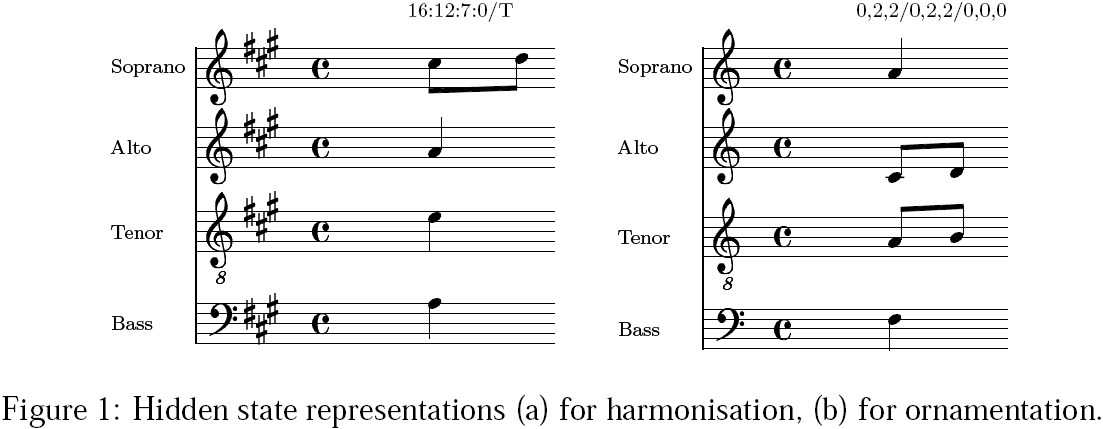
\includegraphics[width=8cm]{allan}}

}

%%%%%%%%%%%%%%%%%%%%%%%%%%%%%%%%%%%%%%%%%%%%%%%%%%%%%%%%%%%%%%%%%%%%%%%%%%%%%%%%

\slide{HMM example: Learning Bach}{

\item results: {\small\url{http://www.anc.inf.ed.ac.uk/demos/hmmbach/}}

~

\centerline{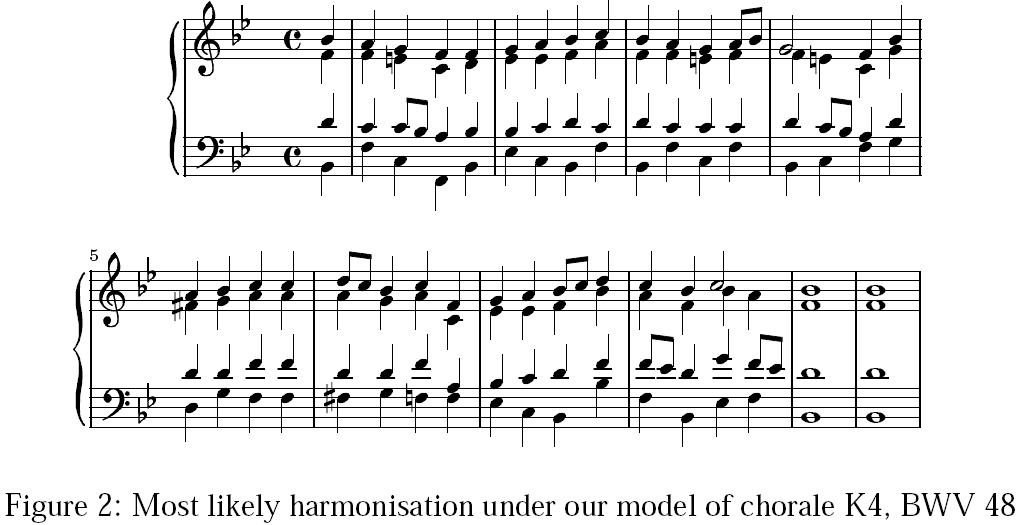
\includegraphics[width=8cm]{allan2}}

~

\item See also work by Gerhard
Widmer \url{http://www.cp.jku.at/people/widmer/}

}

%%%%%%%%%%%%%%%%%%%%%%%%%%%%%%%%%%%%%%%%%%%%%%%%%%%%%%%%%%%%%%%%%%%%%%%%%%%%%%%%

\slide{Dynamic Bayesian Networks}{\label{lastpage}

-- Arbitrary BNs in each time slide

-- Special case: MDPs, speech, etc

}

%%%%%%%%%%%%%%%%%%%%%%%%%%%%%%%%%%%%%%%%%%%%%%%%%%%%%%%%%%%%%%%%%%%%%%%%%%%%%%%%

\slidesfoot

%% \providecommand{\slides}{
  \newcommand{\slideshead}{
  \newcommand{\thepage}{\arabic{mypage}}
  %beamer
  \documentclass[t,hyperref={bookmarks=true}]{beamer}
%  \documentclass[t,hyperref={bookmarks=true},aspectratio=169]{beamer}
  \setbeamersize{text margin left=5mm}
  \setbeamersize{text margin right=5mm}
  \usetheme{default}
  \usefonttheme[onlymath]{serif}
  \setbeamertemplate{navigation symbols}{}
  \setbeamertemplate{itemize items}{{\color{black}$\bullet$}}

  \newwrite\keyfile

  %\usepackage{palatino}
  \stdpackages
  \usepackage{multimedia}

  %%% geometry/spacing issues
  %
  \definecolor{bluecol}{rgb}{0,0,.5}
  \definecolor{greencol}{rgb}{0,.6,0}
  %\renewcommand{\baselinestretch}{1.1}
  \renewcommand{\arraystretch}{1.2}
  \columnsep 0mm

  \columnseprule 0pt
  \parindent 0ex
  \parskip 0ex
  %\setlength{\itemparsep}{3ex}
  %\renewcommand{\labelitemi}{\rule[3pt]{10pt}{10pt}~}
  %\renewcommand{\labelenumi}{\textbf{(\arabic{enumi})}}
  \newcommand{\headerfont}{\helvetica{13}{1.5}{b}{n}}
  \newcommand{\slidefont} {\helvetica{10}{1.4}{m}{n}}
  \newcommand{\codefont} {\helvetica{8}{1.2}{m}{n}}
  \renewcommand{\small} {\helvetica{9}{1.4}{m}{n}}
  \renewcommand{\tiny} {\helvetica{8}{1.3}{m}{n}}
  \newcommand{\ttiny} {\helvetica{7}{1.3}{m}{n}}

  %%% count pages properly and put the page number in bottom right
  %
  \newcounter{mypage}
  \newcommand{\incpage}{\addtocounter{mypage}{1}\setcounter{page}{\arabic{mypage}}}
  \setcounter{mypage}{0}
  \resetcounteronoverlays{page}

  \pagestyle{fancy}
  %\setlength{\headsep}{10mm}
  %\addtolength{\footheight}{15mm}
  \renewcommand{\headrulewidth}{0pt} %1pt}
  \renewcommand{\footrulewidth}{0pt} %.5pt}
  \cfoot{}
  \rhead{}
  \lhead{}
  \lfoot{\vspace*{-3mm}\hspace*{-3mm}\helvetica{5}{1.3}{m}{n}{\texttt{github.com/MarcToussaint/AI-lectures}}}
%  \rfoot{{\tiny\textsf{AI -- \topic -- \subtopic -- \arabic{mypage}/\pageref{lastpage}}}}
%  \rfoot{\vspace*{-4.5mm}{\tiny\textsf{\topic\ -- \subtopic\ -- \arabic{mypage}/\pageref{lastpage}}}\hspace*{-4mm}}
  \rfoot{\vspace*{-4.5mm}{\tiny\textsf{\color{gray}\topic\ -- \subtopic\ -- \arabic{mypage}/\pageref{lastpage}}}\hspace*{-4mm}}
  %\lfoot{\raisebox{5mm}{\tiny\textsf{\slideauthor}}}
  %\rfoot{\raisebox{5mm}{\tiny\textsf{\slidevenue{} -- \arabic{mypage}/\pageref{lastpage}}}}
  %\rfoot{~\anchor{30,12}{\tiny\textsf{\thepage/\pageref{lastpage}}}}
  %\lfoot{\small\textsf{Marc Toussaint}}

  \definecolor{grey}{rgb}{.8,.8,.8}
  \definecolor{head}{rgb}{.85,.9,.9}
  \definecolor{blue}{rgb}{.0,.0,.5}
  \definecolor{green}{rgb}{.0,.5,.0}
  \definecolor{red}{rgb}{.8,.0,.0}
  \newcommand{\inverted}{
    \definecolor{main}{rgb}{1,1,1}
    \color{main}
    \pagecolor[rgb]{.3,.3,.3}
  }
  \input{../shared/macros}

  \graphicspath{{pics/}{../shared/pics/}}

  \title{Machine Learning \topic}
  \author{Marc Toussaint}
  \institute{Machine Learning \& Robotics Lab, U Stuttgart}

  \begin{document}

  \rfoot{\vspace*{-5mm}{\tiny
  \textsf{\arabic{mypage}/\pageref{lastpage}}}\hspace*{-4mm}}

  %% title slide!
  \slide{}{
    \thispagestyle{empty}

    \twocol{.27}{.6}{
      \hspace*{-15mm}\includegraphics[height=7cm]{classPicture2-bw}
    }{\center

      \textbf{\fontsize{17}{20}\selectfont \course}

      ~

      %Lecture
      \topic\\

      \vspace{1cm}

      {\tiny~\emph{\keywords}~\\}

      \vspace{1cm}

      Marc Toussaint
      
      University of Stuttgart

      Summer 2019

      ~

    }
  }
}

\newcommand{\slide}[2]{
  \slidefont
  \incpage\begin{frame}
  \addcontentsline{toc}{section}{#1}
  \vfill
  {\headerfont #1} \vspace*{-2ex}
  \begin{itemize}\item[]~\\
    #2
  \end{itemize}
  \vfill
  \end{frame}
}

\newenvironment{slidecore}[1]{
  \slidefont\incpage
  \addcontentsline{toc}{section}{#1}
  \vfill
  {\headerfont #1} \vspace*{-2ex}
  \begin{itemize}\item[]~\\
}{
  \end{itemize}
  \vfill
}


\providecommand{\key}[1]{
  \addtocounter{mypage}{1}
% \immediate\write\keyfile{#1}
  \addtocontents{toc}{\hyperref[key:#1]{#1 (\arabic{mypage})}}
%  \phantomsection\label{key:#1}
%  \index{#1@{\hyperref[key:#1]{#1 (\arabic{mysec}:\arabic{mypage})}}|phantom}
  \addtocounter{mypage}{-1}
}

\providecommand{\course}{}

\providecommand{\subtopic}{}

\providecommand{\sublecture}[2]{
  \renewcommand{\subtopic}{#1}
  \slide{#1}{#2}
}

\providecommand{\story}[1]{
~

Motivation: {\tiny #1}\clearpage
}

\newenvironment{items}[1][9]{
\par\setlength{\unitlength}{1pt}\fontsize{#1}{#1}\linespread{1.2}\selectfont
\begin{list}{--}{\leftmargin4ex \rightmargin0ex \labelsep1ex \labelwidth2ex
\topsep0pt \parsep0ex \itemsep3pt}
}{
\end{list}
}

\providecommand{\slidesfoot}{
  \end{document}
}


  \slideshead
}

\providecommand{\exercises}{
  \newcommand{\exerciseshead}{
  \documentclass[10pt,fleqn]{article}
  \stdpackages

  \definecolor{bluecol}{rgb}{0,0,.5}
  \definecolor{greencol}{rgb}{0,.4,0}
  \definecolor{shadecolor}{gray}{0.9}
  \usepackage[
    %    pdftex%,
    %%    letterpaper,
    %    bookmarks,
    %    bookmarksnumbered,
    colorlinks,
    urlcolor=bluecol,
    citecolor=black,
    linkcolor=bluecol,
    %    pagecolor=bluecol,
    pdfborder={0 0 0},
    %pdfborderstyle={/S/U/W 1},
    %%    backref,     %link from bibliography back to sections
    %%    pagebackref, %link from bibliography back to pages
    %%    pdfstartview=FitH, %fitwidth instead of fit window
    pdfpagemode=UseNone, %UseOutlines, %bookmarks are displayed by acrobat
    pdftitle={\course},
    pdfauthor={Marc Toussaint},
    pdfkeywords={}
  ]{hyperref}
  \DeclareGraphicsExtensions{.pdf,.png,.jpg,.eps}

  \renewcommand{\r}{\varrho}
  \renewcommand{\l}{\lambda}
  \renewcommand{\L}{\Lambda}
  \renewcommand{\b}{\beta}
  \renewcommand{\d}{\delta}
  \renewcommand{\k}{\kappa}
  \renewcommand{\t}{\theta}
  \renewcommand{\O}{\Omega}
  \renewcommand{\o}{\omega}
  \renewcommand{\SS}{{\cal S}}
  \renewcommand{\=}{\!=\!}
  %\renewcommand{\boldsymbol}{}
  %\renewcommand{\Chapter}{\chapter}
  %\renewcommand{\Subsection}{\subsection}

  \renewcommand{\baselinestretch}{1.1}
  \geometry{a4paper,headsep=7mm,hdivide={15mm,*,15mm},vdivide={20mm,*,15mm}}

  \fancyhead[L]{\thetitle, \textit{Marc Toussaint}---\today}
  \fancyhead[R]{\thepage}
  \fancyhead[C]{}
  \fancyfoot{}
  \pagestyle{fancy}

  \parindent 0pt
  \parskip 0.5ex

  \newcommand{\codefont}{\helvetica{8}{1.2}{m}{n}}

  \input{../shared/macros}

  \DefineShortVerb{\@}

  \newcounter{solutions}
  \setcounter{solutions}{1}
  \newenvironment{solution}{
    \small
    \begin{shaded}
  }{
    \end{shaded}
  }
  
  \renewcommand{\hat}{\widehat}
  \newcommand{\bbg}{{\bar{\bar g}}}
  \graphicspath{{pics/}{../shared/pics/}}

  \renewcommand{\labelenumi}{{\alph{enumi})}}

  %%%%%%%%%%%%%%%%%%%%%%%%%%%%%%%%%%%%%%%%%%%%%%%%%%%%%%%%%%%%%%%%%%%%%%%%%%%%%%%%


  \mytitle{\course\\Exercise \exnum}
  \myauthor{Marc Toussaint\\ TAs: Janik Hager, Philipp Kratzer\\\small\addressUSTT}
  
  
  \begin{document}
  \onecolumn
  \maketitle
}

\newcommand{\exsection}[1]{\section{#1}}

\newcommand{\exerfoot}{
  \end{document}
}

\newenvironment{items}[1][9]{
  \par\setlength{\unitlength}{1pt}\fontsize{#1}{#1}\linespread{1.2}\selectfont
  \begin{list}{--}{\leftmargin4ex \rightmargin0ex \labelsep1ex \labelwidth2ex
      \topsep0pt \parsep0ex \itemsep3pt}
}{
  \end{list}
}

  \exerciseshead
}

\providecommand{\script}{
  \newcommand{\scripthead}{
  \documentclass[9pt,twoside]{article}
  \stdpackages

  \usepackage{palatino}
  \usepackage[envcountsect]{beamerarticle}
  \usepackage{makeidx}
  \makeindex

  \definecolor{bluecol}{rgb}{0,0,.5}
  \definecolor{greencol}{rgb}{0,.4,0}
  \definecolor{shadecolor}{gray}{0.9}
  \usepackage[
    %    pdftex%,
    %%    letterpaper,
    %bookmarks,
    bookmarksnumbered,
    colorlinks,
    urlcolor=bluecol,
    citecolor=black,
    linkcolor=bluecol,
    %    pagecolor=bluecol,
    pdfborder={0 0 0},
    %pdfborderstyle={/S/U/W 1},
    %%    backref,     %link from bibliography back to sections
    %%    pagebackref, %link from bibliography back to pages
    %%    pdfstartview=FitH, %fitwidth instead of fit window
    pdfpagemode=UseOutlines, %bookmarks are displayed by acrobat
    pdftitle={\course},
    pdfauthor={Marc Toussaint},
    pdfkeywords={}
  ]{hyperref}
  \DeclareGraphicsExtensions{.pdf,.png,.jpg,.eps}

  \usepackage{multimedia}
  %\setbeamercolor{background canvas}{bg=}

  \renewcommand{\r}{\varrho}
  \renewcommand{\l}{\lambda}
  \renewcommand{\L}{\Lambda}
  \renewcommand{\b}{\beta}
  \renewcommand{\d}{\delta}
  \renewcommand{\k}{\kappa}
  \renewcommand{\t}{\theta}
  \renewcommand{\O}{\Omega}
  \renewcommand{\o}{\omega}
  \renewcommand{\SS}{{\cal S}}
  \renewcommand{\=}{\!=\!}
  %\renewcommand{\boldsymbol}{}
  %\renewcommand{\Chapter}{\chapter}
  %\renewcommand{\Subsection}{\subsection}

  \renewcommand{\baselinestretch}{1.0}
  \geometry{a5paper,headsep=6mm,hdivide={10mm,*,10mm},vdivide={13mm,*,7mm}}

  \fancyhead[OL,ER]{\course, \textit{Marc Toussaint}}
  \fancyhead[OR,EL]{\thepage}
  \fancyhead[C]{}
  \fancyfoot{}
  \pagestyle{fancy}

%  \setcounter{tocdepth}{3}
  \setcounter{tocdepth}{2}

   \columnsep 6ex
  %  \renewcommand{\familydefault}{\sfdefault}
  \newcommand{\headerfont}{\large}%helvetica{12}{1}{b}{n}}
  \newcommand{\slidefont} {}%\helvetica{9}{1.3}{m}{n}}
  \newcommand{\storyfont} {}
  %  \renewcommand{\small}   {\helvetica{8}{1.2}{m}{n}}
  \renewcommand{\tiny}    {\footnotesize}%helvetica{7}{1.1}{m}{n}}
  \newcommand{\codefont}{\fontsize{6}{6}\selectfont}%helvetica{8}{1.2}{m}{n}}

  \input{../shared/macros}

  \DefineShortVerb{\@}

  \newcounter{solutions}
  \setcounter{solutions}{1}
  \renewenvironment{solution}{
    \small
    \begin{shaded}
  }{
    \end{shaded}
  }

  \graphicspath{{pics/}{../shared/pics/}}

%%%%%%%%%%%%%%%%%%%%%%%%%%%%%%%%%%%%%%%%%%%%%%%%%%%%%%%%%%%%%%%%%%%%%%%%%%%%%%%%

  \mytitle{\course\\Lecture Script}
  \myauthor{Marc Toussaint}
  \date{\coursedate}

  \begin{document}

  %% \vspace*{2cm}

  \maketitle
  %\anchor{100,10}{\includegraphics[width=4cm]{optim}}

%  \vspace*{1cm}

  \emph{This is a direct concatenation and reformatting of all lecture
    slides and exercises from this course, including indexing to help
    prepare for exams.}

  {\tableofcontents}
}

%%%%%%%%%%%%%%%%%%%%%%%%%%%%%%%%%%%%%%%%%%%%%%%%%%%%%%%%%%%%%%%%%%%%%%%%%%%%%%%%

%% \renewcommand{\keywords}{}
%% \newcommand{\topic}{}
%% \renewcommand{\mypause}{}

  \newcounter{mypage}
  \setcounter{mypage}{0}
  \newcounter{mysec}
  \setcounter{mysec}{0}
  \newcommand{\incpage}{\addtocounter{mypage}{1}}
  \newcommand{\incsec} {\addtocounter{mysec}{1}}

\newcommand{\beginTocMinipage}{
  \addtocontents{toc}{\smallskip\noindent\hspace*{.036\columnwidth}}
  \addtocontents{toc}{\protect\begin{minipage}{.914\columnwidth}\small}
}
\newcommand{\closeTocMinipage}{
  \addtocontents{toc}{\protect\end{minipage}}
  \addtocontents{toc}{}
  \addtocontents{toc}{\medskip}
}

\renewcommand{\slides}[1][]{
  \clearpage
  \incsec
  \section{\topic}
  {\small #1}
  \beginTocMinipage
  \setcounter{mypage}{0}
  \smallskip\nopagebreak\hrule\medskip
}

\newcommand{\slidesfoot}{
  \closeTocMinipage
  \bigskip
}

\newcommand{\sublecture}[2]{
  \pagebreak[3]
  \incpage
  \closeTocMinipage
  \subsection{#1}
  {\storyfont #2}
  \beginTocMinipage
  {\hfill\tiny \textsf{\arabic{mysec}:\arabic{mypage}}}\nopagebreak%
  \smallskip\nopagebreak\hrule
}

\newcommand{\key}[1]{
  \pagebreak[2]
  \addtocounter{mypage}{1}
  \addtocontents{toc}{\hyperref[key:#1]{#1 (\arabic{mysec}:\arabic{mypage})}}
  \phantomsection\label{key:#1}
  \index{#1@{\hyperref[key:#1]{#1 (\arabic{mysec}:\arabic{mypage})}}|phantom}
  \addtocounter{mypage}{-1}
}

\newenvironment{slidecore}[1]{
  \incpage
  \subsubsection*{#1}%{\headerfont\noindent\textbf{#1}\\}%
  \vspace{-6ex}%
  \begin{list}{$\bullet$}{\leftmargin4ex \rightmargin0ex \labelsep1ex
    \labelwidth2ex \partopsep0ex \topsep0ex \parsep.5ex \parskip0ex \itemsep0pt}\item[]~\\\nopagebreak%
}{
  \end{list}\nopagebreak%
  {\hfill\tiny \textsf{\arabic{mysec}:\arabic{mypage}}}\nopagebreak%
  \smallskip\nopagebreak\hrule
}

\newcommand{\slide}[2]{
  \begin{slidecore}{#1}
    #2
  \end{slidecore}
}

\newcommand{\exsection}[1]{
  \subsubsection{#1}
}

\renewcommand{\exercises}{
  \subsection{Exercise \exnum}
}

\newcommand{\exerfoot}{
  \bigskip
}

\newcommand{\story}[1]{
  \subsection*{Motivation \& Outline}
  \addtocontents{toc}{\hyperref[mot\arabic{mysec}]{Motivation \& Outline}}
  \phantomsection\label{mot\arabic{mysec}}
  {\storyfont\sf #1}
  \medskip\nopagebreak\hrule
}

\newcounter{savedsection}
\newcommand{\subappendix}{\setcounter{savedsection}{\arabic{section}}\appendix}
\newcommand{\noappendix}{
  \setcounter{section}{\arabic{savedsection}}% restore section number
  \setcounter{subsection}{0}% reset section counter
%  \gdef\@chapapp{\sectionname}% reset section name
  \renewcommand{\thesection}{\arabic{section}}% make section numbers arabic
}

\newenvironment{items}[1][9]{
\par\setlength{\unitlength}{1pt}\fontsize{#1}{#1}\linespread{1.2}\selectfont
\begin{list}{--}{\leftmargin4ex \rightmargin0ex \labelsep1ex \labelwidth2ex
\topsep0pt \parsep0ex \itemsep3pt}
}{
\end{list}
}

  \scripthead
}

\providecommand{\course}{NO COURSE}
\providecommand{\topic}{NO TOPIC}
\providecommand{\keywords}{NO KEYWORDS}
\providecommand{\exnum}{NO NUMBER}


\providecommand{\stdpackages}{
  \usepackage{amsmath}
  \usepackage{amssymb}
  \usepackage{amsfonts}
  \allowdisplaybreaks
  \usepackage{amsthm}
  \usepackage{eucal}
  \usepackage{graphicx}
  \usepackage{color}
  \usepackage{geometry}
  \usepackage{framed}
%  \usecolor{xcolor}
  \definecolor{shadecolor}{gray}{0.9}
  \setlength{\FrameSep}{3pt}
  \usepackage{fancyvrb}
  \fvset{numbers=left,xleftmargin=5ex}

  \usepackage{multicol} 
  \usepackage{fancyhdr}
}

\providecommand{\addressUSTT}{
  Machine~Learning~\&~Robotics~lab, U~Stuttgart\\\small
  Universit{\"a}tsstra{\ss}e 38, 70569~Stuttgart, Germany
}


\renewcommand{\course}{Artificial Intelligence}
\renewcommand{\coursepicture}{course_ai}
\renewcommand{\coursedate}{Winter 2019}
\renewcommand{\topic}{AI \& Machine Learning \& Neural Nets}
\renewcommand{\keywords}{}

\slides

%%%%%%%%%%%%%%%%%%%%%%%%%%%%%%%%%%%%%%%%%%%%%%%%%%%%%%%%%%%%%%%%%%%%%%%%%%%%%%%%

\story{

Neural networks became a central topic for Machine Learning and
AI. But in principle, they're just parameterized functions that can be
fit to data. They lack many appealing aspects that were the focus of
ML research in the '90-'10. So why are they so successful now? This
lecture introduces the basics and tries to discuss the success of NNs.

}

%%%%%%%%%%%%%%%%%%%%%%%%%%%%%%%%%%%%%%%%%%%%%%%%%%%%%%%%%%%%%%%%%%%%%%%%%%%%%%%%

\sublecture{What is AI?}{
}

%%%%%%%%%%%%%%%%%%%%%%%%%%%%%%%%%%%%%%%%%%%%%%%%%%%%%%%%%%%%%%%%%%%%%%%%%%%%%%%%

\slide{What is AI?}{

\item AI is a research field

~%\pause

\item AI research is about systems that take decisions
\begin{items}
\item AI formalizes decision processes: interactive (decisions change world state), or passive
\item AI distinguishes between agent(s) and the external world: decision variables
\end{items}

~%\pause

\item ... systems that take optimal/desirable decisions
\begin{items}
\item AI formalizes decision objectives
\item AI aims for systems to exhibit functionally \emph{desirable behavior}
\end{items}

~%\pause

\item ... systems that take optimal decisions on the basis of all available information
\begin{items}
\item AI is about inference
\item AI is about learning
\end{items}

}

%%%%%%%%%%%%%%%%%%%%%%%%%%%%%%%%%%%%%%%%%%%%%%%%%%%%%%%%%%%%%%%%%%%%%%%%%%%%%%%%

\slide{What is Machine Learning?}{

\item In large parts, ML is: \quad (let's call this ML$^0$)

\cen{\emph{Fitting a function $f: x\mapsto y$ to given data $D=\{ (x_i,y_i) \}_{i=1}^n$}}

~\pause

\item And what does that have to do with AI?

\item Taken literally, not much:
\begin{items}
\item The decision made by a ML$^0$ method is only a single decision: Decide on the function $f\in\HH$ in the hypothesis space $\HH$

\item This ``single-decision process'' is not interactive; ML$^0$ does not formalize/model/consider how the choice of $f$ changes the world

\item The objective $\LL(f, D)$ in ML$^0$ depends only on the given static data $D$ and the decision $f$, not how $f$ might change the world

\item ``Learning'' in ML$^0$ is not an interactive process, but some method to pick $f$ on the basis of the static $D$. The typically iterative optimization process is not the decision process that ML$^0$ focusses on.
\end{items}

}

%%%%%%%%%%%%%%%%%%%%%%%%%%%%%%%%%%%%%%%%%%%%%%%%%%%%%%%%%%%%%%%%%%%%%%%%%%%%%%%%

\slide{}{

\textbf{But,} function approximation can be used to help solving AI (interactive decision process) problems:

\item Building a trained/fixed $f$ into an interacting system based on human expert knowledge

\smallskip

{\tiny E.g., an engineer trains a NN $f$ to recognize street signs based on
a large fixed data set $D$. S/he builds $f$ into a car to drive
autonomously. That car certainly solves an AI problem; $f$
continuously makes decisions that change the state of the world. But
$f$ was never optimized literally for the task of interacting with the
world; it was only optimized to minimze a loss on the static data
$D$. It is not a priori clear that minimizing the loss of $f$ on $D$
is related to maximizing rewards in car driving. That fact is the
expertise of the engineer; it is not some AI algorithm that discovered
that fact. At no place there was an AI method that ``learns to drive a
car''. There was only an optimization method to minimize the loss of
$f$ on $D$.

}

\item Using ML in interactive decision processes

\smallskip

{\tiny
E.g., to approximate a $Q$-function, state evaluation function, reward
function, the system dynamics, etc. Then, other AI methods can use
these approximate models to actually take decisions in the interactive
context.

}

}

%%%%%%%%%%%%%%%%%%%%%%%%%%%%%%%%%%%%%%%%%%%%%%%%%%%%%%%%%%%%%%%%%%%%%%%%%%%%%%%%

\slide{[Machine Learning beyond ML$^0$]}{

\item Many areas of ML go beyond plain function approximation:

~

\item Fitting more structured models to data, which includes
\begin{items}
\item Time series, recurrent processes
\item Graphical Models
\item Unsupervised learning (semi-supervised learning)
\end{items}
{\small
...but in all these cases, the scenario is still not interactive, the data $D$ is static, the decision is about picking a single model $f$ from a hypothesis space, and the objective is a loss based on $f$ and $D$ only.

}

\item Active Learning, where the ``ML agent'' makes decisions about what data label to query next

\item Bandits

\item Reinforcement Learning ~ {\tiny(roughly, marriage of ML and decision theory)}

}

%%%%%%%%%%%%%%%%%%%%%%%%%%%%%%%%%%%%%%%%%%%%%%%%%%%%%%%%%%%%%%%%%%%%%%%%%%%%%%%%

\sublecture{Machine Learning primer}{

\item Basic ML$^0$ (function approximation) is all about specifying the
\begin{items}
\item \textbf{Model:} How is the function $f:x\mapsto y$ represented/parameterized?
\item \textbf{Objective:} Given a data set $D$, what loss should $f$ minimize?
\item \textbf{Solver:} What algorithm do we use to minimize the loss?
\end{items}

~\pause

\item Given data $D=\{ (x_i,y_i) \}_{i=1}^n$, the standard objective is to minimize the ``error'' on the data
\begin{align*}
f^* \argmin _{f\in\HH} \sum_{i=1}^n \ell(f(x_i), y_i) ~,
\end{align*}
where $\ell(\hat y, y) > 0$ penalizes a discrepancy between a model output $\hat y$ and the data $y$.

\begin{items}
\item Squared error $\ell(\hat y, y) = (\hat y - y)^2$
\item Classification error $\ell(\hat y, y) = [ \hat y \not= y ]$
\item neg-log likelihood $\ell(\hat y, y) = -\log p(y \| \hat y)$
\item etc
\end{items}

}

%%%%%%%%%%%%%%%%%%%%%%%%%%%%%%%%%%%%%%%%%%%%%%%%%%%%%%%%%%%%%%%%%%%%%%%%%%%%%%%%

\slide{Example: Polynomial Ridge Regression}{

\item \textbf{Model:} Given input $x\in\RRR^d$ and output $y\in\RRR$, we represent functions $f_\b$ as polynomials over $x$,
$$f(x) = \sum_{j=1}^k \phi_j(x)~ \b_j = \phi(x)^\T \b$$
where $\phi(x)$ is the \textbf{feature} vector of all monomials, e.g.\ quadratic:
$\phi(x) = (1,x_1,..,x_d,x_1^2,x_1x_2,x_1x_3,..,x_d^2)$

~\pause

\item \textbf{Objective:} Given data $D=\{(x_i,y_i)\}_{i=1}^n$ we define the loss as
$$L^{\text{ridge}}(\b) = \sum_{i=1}^n (y_i - \phi(x_i)^\T \b)^2 + \l \sum_{j=2}^k \b_j^2$$

~\pause

\item \textbf{Solver:} We can solve this analytically:
$$\hat \b^\text{ridge} = \argmin_\b L^\text{ridge}(\b) = (X^\T X + \l I)^\1 X^\T y$$

{\tiny where $y=(y_1,..,y_n)$ is the vector of outputs, and $X_{i\cdot} = \phi(x_i)$ contains the feature vectors in rows.

}
}

%%%%%%%%%%%%%%%%%%%%%%%%%%%%%%%%%%%%%%%%%%%%%%%%%%%%%%%%%%%%%%%%%%%%%%%%%%%%%%%%

\sublecture{Neural Networks}{
}

%%%%%%%%%%%%%%%%%%%%%%%%%%%%%%%%%%%%%%%%%%%%%%%%%%%%%%%%%%%%%%%%%%%%%%%%%%%%%%%%

\slide{What is a Neural Network?}{

\item A NN is a parameterized function $f_\b: \RRR^d \mapsto \RRR^M$
\begin{items}
\item $\b$ are called weights
\item Given a data set $D=\{(x_i,y_i)\}_{i=1}^n$, we minimize some loss
$$\beta^* = \argmin_\b \sum_{i=1}^n \ell(f_\b(x_i), y_i) + \text{~regularization}$$
\end{items}

\item In that sense, they just replace our previous model assumption $f(x) = \phi(x)^\T \b$, the reset is ``in principle'' the same

}

%%%%%%%%%%%%%%%%%%%%%%%%%%%%%%%%%%%%%%%%%%%%%%%%%%%%%%%%%%%%%%%%%%%%%%%%%%%%%%%%

\key{Neural Network function class}
\slide{Neural Network models}{

\item A (fwd-forward) NN $\RRR^{h_0} \mapsto \RRR^{h_L}$ with $L$ layers, each $h_l$-dimensional, defines the function
\begin{tabular}{l@{~}l@{~}l}
1-layer: & $f_\b(x) = W_1 x + b_1$, & $W_1 \in \RRR^{h_1\times h_0}, b_1\in\RRR^{h_1}$ \\
2-layer: & $f_\b(x) = W_2 \s(W_1 x+b_1) + b_2$, & $W_l \in \RRR^{h_l\times h_{l\1}}, b_l\in\RRR^{h_l}$ \\
$L$-layer: & $f_\b(x) = W_L \s(\cdots \s(W_1 x+b_1) \cdots) + b_L$\hspace*{-5mm}
\end{tabular}

~

\item The parameter $\b=(W_{1:L}, b_{1:L})$ is the collection of all\\
\textbf{weights} $W_l \in \RRR^{h_l\times h_{l\1}}$ and \textbf{biases} $b_l\in\RRR^{h_l}$

}

%%%%%%%%%%%%%%%%%%%%%%%%%%%%%%%%%%%%%%%%%%%%%%%%%%%%%%%%%%%%%%%%%%%%%%%%%%%%%%%%

\slide{}{

\only<1>{\show{NeuralNet-new-regression}}
\only<2>{\show{NeuralNet-new-classification}}
\only<3>{\show{NeuralNet-new-NN}}

}

%%%%%%%%%%%%%%%%%%%%%%%%%%%%%%%%%%%%%%%%%%%%%%%%%%%%%%%%%%%%%%%%%%%%%%%%%%%%%%%%

\slide{Neural Network models}{

\item To describe the mapping as an iteration, we introduce notation for the intermediate values:
\begin{items}
\item the \textbf{input} to layer $l$ is $z_l = W_l x_{l\1} + b_l \in \RRR^{h_l}$
\item the \textbf{activation} of layer $l$ is $x_l = \s(z_l) \in \RRR^{h_l}$
\end{items}

\item Then the $L$-layer NN model can be computed using the \textbf{forward propagation:} 
$$\forall_{l=1,..,L\1}:~ z_l = W_l x_{l\1} + b_l \comma x_l=\s(z_l)$$
where $x_0\equiv x$ is the input, and $f_\b(x) \equiv z_L$ the output

~

\begin{items}
\item $x_{l\1}\mapsto z_l$ is a linear transformation, highly parameterized with $W_l,b_l$
\item $z_l\mapsto x_l$ is a non-linear transformation, element-wise and without parameters
\end{items}

~

\item $L$-layer means $L-1$ hidden layers plus 1 output layer. (The input $x_0$ is not counted.)

}

%%%%%%%%%%%%%%%%%%%%%%%%%%%%%%%%%%%%%%%%%%%%%%%%%%%%%%%%%%%%%%%%%%%%%%%%%%%%%%%%

\slide{Neural Network models}{

\item The \textbf{activation function} $\s(z)$ is applied \emph{element-wise},

{\small
\begin{tabular}{ll}
rectified linear unit (ReLU) & $\s(z) = [z]_+ = \max\{0,z\} = z [z\ge 0]$\\
leaky ReLU & $\s(z) = \max\{0.01z, z\} =  \begin{cases} 0.01 z & z<0 \\ z & z\ge 0\end{cases}$\\
sigmoid, logistic & $\s(z) = 1/(1+e^{-z})$ \\
tanh & $\s(z) = \tanh(z)$
\end{tabular}
}

}

%%%%%%%%%%%%%%%%%%%%%%%%%%%%%%%%%%%%%%%%%%%%%%%%%%%%%%%%%%%%%%%%%%%%%%%%%%%%%%%%

\slide{Neural Network models}{

\item We can think of the second-to-last layer $x_{L\1}$ as a feature vector
$$\phi_\b(x) = x_{L\1}$$

\item This aligns NNs models with what we discussed so far. But the crucial difference is:

\cen{\textbf{In NNs, the features $\phi_\b(x)$ are also parameterized and trained!}}

While in previous lectures, we had to fix $\phi(x)$ by hand, NNs allow us to learn features and \textbf{intermediate representations}

~\tiny

\item Note: It is a common approach to train NNs as usual, but after training fix the trained features $\phi(x)$ (``remove the head (=output layer) and fix the remaining body of the NN'') and use these trained features for similar problems or other kinds of ML on top.

}

%%%%%%%%%%%%%%%%%%%%%%%%%%%%%%%%%%%%%%%%%%%%%%%%%%%%%%%%%%%%%%%%%%%%%%%%%%%%%%%%

\slide{NNs as unversal function approximators}{

\item A 1-layer NN is linear in the input

\item Already a 2-layer NN with $h_1\to \infty$ hidden neurons is a universal function approximator
\begin{items}
\item Corresponds to $k\to\infty$ features $\phi(x)\in\RRR^k$ that are well tuned
\end{items}

}

%%%%%%%%%%%%%%%%%%%%%%%%%%%%%%%%%%%%%%%%%%%%%%%%%%%%%%%%%%%%%%%%%%%%%%%%%%%%%%%%

\slide{Objectives to train NNs}{
}

%%%%%%%%%%%%%%%%%%%%%%%%%%%%%%%%%%%%%%%%%%%%%%%%%%%%%%%%%%%%%%%%%%%%%%%%%%%%%%%%

\key{NN loss functions}
\slide{Loss functions as usual}{

\item Squared error regression, for $h_L$-dimensional output:
\begin{items}
\item for a single data point $(x,y^*)$, $\ell(f(x),y^*) = (f(x) - y^*)^2$

\item the loss gradient is $\frac{\del\ell}{\del f} = 2 (f-y^*)^\T$
\end{items}

~

\item For multi-class classification we have $h_L=M$ outputs, and $f_\beta(x)\in\RRR^M$ represents the \emph{discriminative function},
which means that the predicted class is the $\argmax_{y\in\{1,..,M\}}
[f_\t(x)]_y$.

\item Neg-log-likelihood or cross entropy loss:
\begin{items}
\item for a single data point $(x,y^*)$, $\ell(f(x),y^*) = -\log p(y^* | x)$

\item the loss gradient at output $y$ is $\frac{\del\ell}{\del f_y} = p(y|x) - [y=y^*]$
\end{items}

\item One-vs-all hinge loss:
\begin{items}
\item for a single data point $(x,y^*)$, $\ell(f(x),y^*) = \sum_{y\not=y^*} [1 - (f_{y^*}-f_y)]_+$,

\item the loss gradient at non-target outputs $y\not=y^*$ is $\frac{\del\ell}{\del f_y} = [f_{y^*} < f_y+1 ]$

\item the loss gradient at the target output $y^*$ is $\frac{\del\ell}{\del f_{y^*}} = -\sum_{y\not=y^*} [f_{y^*} < f_y+1]$

\item this is also called \textbf{Perceptron Algorithm}
\end{items}

}

%%%%%%%%%%%%%%%%%%%%%%%%%%%%%%%%%%%%%%%%%%%%%%%%%%%%%%%%%%%%%%%%%%%%%%%%%%%%%%%%

\key{NN regularization}
\key{NN Dropout}
\slide{New types of regularization}{

\item Conventionally: add a $L_2$ or $L_1$ regularization.
\begin{items}
\item adds a penalty $\l W_{l,ij}^2$ (Ridge) or $\l|W_{l,ij}|$ (Lasso) for every weight
\item In practise, compute the unregularized gradient as usual, then add $\l W_{l,ij}$ (for $L_2$),
or $\l\sign{W_{l,ij}}$ (for $L_1$) to the gradient
\item Historically, this is called \textbf{weight decay}, as the additional gradient (executed after the unregularized weight update) just decays weights
\end{items}

\item Core modern approach: Dropout
\begin{items}
\item (see next slide)
\end{items}

\item Others:
\begin{items}
\item Data Augmentation
\item Training ensembles, bagging (averaging bootstrapped models)
\item Additional embedding objectives (e.g.\ semi-supervised embedding)
\item Early stopping
\end{items}

}

%%%%%%%%%%%%%%%%%%%%%%%%%%%%%%%%%%%%%%%%%%%%%%%%%%%%%%%%%%%%%%%%%%%%%%%%%%%%%%%%

\slide{Dropout}{

\item What is dropout?

\begin{items}
\item During both, forward passing and gradient computation, pretend that randomly selected ``neurons'' would not exist
\item For each entry $i$ in each layer $x_{l,i}$, decide with probability $p$ ($\approx .5$) whether it drops out: set the respective activation $x_{l,i}$, and gradient $\l_{l,i}$, equal to zero
\item At prediction time, ``average'' dropouts, i.e., multiply each activation $x_{l,i}$ with $p$
\end{items}

\item Theoretial foundation?
\begin{items}
\item Each dropout pattern defines another network. We have a random ensemble of networks, sharing parameters, each of which is trained on the same task. Eventually, we want to average of this ensemble.
\item \emph{Srivastava et al: Dropout: a simple way to prevent neural networks from overfitting, JMLR 2014.}
\item ``a way  of  approximately  combining  exponentially  many  different  neural  network architectures efficiently''
\item ``$p$ can  simply  be  set  at  0.5,  which  seems  to  be  close  to  optimal  for  a  wide  range  ofnetworks and tasks''
%\item on test/prediction time, take true averages
\end{items}
}

}

%%%%%%%%%%%%%%%%%%%%%%%%%%%%%%%%%%%%%%%%%%%%%%%%%%%%%%%%%%%%%%%%%%%%%%%%%%%%%%%%

%% \key{data augmentation}
%% \slide{Data Augmentation}{

%% \item A very interesting form of regularization is to modify the data!

%% \item Generate more data by applying invariances to the given data. The model then learns to generalize as described by these invariances.

%% \item This is a form of regularization that directly incorporates expert knowledge

%% ~

%% \show[.6]{dataAugmentation}

%% }

%%%%%%%%%%%%%%%%%%%%%%%%%%%%%%%%%%%%%%%%%%%%%%%%%%%%%%%%%%%%%%%%%%%%%%%%%%%%%%%%

\slide{Optimization}{
}

%%%%%%%%%%%%%%%%%%%%%%%%%%%%%%%%%%%%%%%%%%%%%%%%%%%%%%%%%%%%%%%%%%%%%%%%%%%%%%%%

\key{NN gradient}
\key{NN back propagation}
\slide{Computing the gradient}{

\item Recall \textbf{forward propagation} in an $L$-layer NN:
$$\forall_{l=1,..,L\1}:~ z_l = W_l x_{l\1} + b_l \comma x_l=\s(z_l)$$

\item For a single data point $(x,y^*)$, assume we have a loss $\ell(f(x),y^*)$

We define $\d_L \defeq \frac{d \ell}{d f} = \frac{d \ell}{d z_L} \in\RRR^{1\times M}$ as the gradient (as row vector) w.r.t.\ output values $z_L$.

\item \textbf{Backpropagation:} We can recursivly compute the gradient $\frac{d \ell}{d z_l} \in\RRR^{1\times h_l}$ w.r.t.\ all other layers $z_l$ as:
\begin{align*}
\forall_{l=L\1,..,1}:~ \d_l
&\defeq \frac{d \ell}{d z_l} 
 = \frac{d \ell}{d z_{l\po}} \frac{\del z_{l\po}}{\del x_l} \frac{\del x_l}{\del z_l}
 = [\d_{l\po}~ W_{l\po}] \circ [\s'(z_l)]^\T
\end{align*}
where $\circ$ is an \emph{element-wise product}. The gradient w.r.t.\ parameters:
\begin{align*}
\frac{d \ell}{d W_{l,ij}}
 &= \frac{d \ell}{d z_{l,i}}~ \frac{\del z_{l,i}}{\del W_{l,ij}}
  = \d_{l,i}~ x_{l\1,j}\quad \text{or}\quad
\frac{d \ell}{d W_l}
  = \d_l^\T x_{l\1}^\T
\comma   \frac{d \ell}{d b_l} = \d_l^\T
\end{align*}

}

%%%%%%%%%%%%%%%%%%%%%%%%%%%%%%%%%%%%%%%%%%%%%%%%%%%%%%%%%%%%%%%%%%%%%%%%%%%%%%%%

\slide{}{

\item This forward and backward computations are done for each data point $(x_i,y_i)$.

\item Since the total loss is the sum $L(\b) = \sum_i \ell(f_\b(x_i), y_i)$, the total gradient is the sum of gradients per data point.

\item Efficient implementations send multiple data points (tensors) simultaneously through the network (fwd and bwd), which speeds up computations.

}

%%%%%%%%%%%%%%%%%%%%%%%%%%%%%%%%%%%%%%%%%%%%%%%%%%%%%%%%%%%%%%%%%%%%%%%%%%%%%%%%

\slide{Optimization}{

\item For small data size:

We can compute the loss and its gradient $\sum_{i=1}^n \nabla_\b \ell(f_\b(x_i), y_i)$.
\begin{items}
\item Use classical gradient-based optimization methods
\item default: L-BFGS, oldish but efficient: Rprop
\item Called \textbf{batch learning} ~ (in contrast to online learning)
\end{items}

~

\item For large data size: \quad The $\sum_{i=1}^n$ is highly inefficient!
\begin{items}
\item Adapt weights based on much smaller data subsets, \textbf{mini batches}
\end{items}

}

%%%%%%%%%%%%%%%%%%%%%%%%%%%%%%%%%%%%%%%%%%%%%%%%%%%%%%%%%%%%%%%%%%%%%%%%%%%%%%%%

\key{Stochastic Gradient Descent}
\slide{Stochastic Gradient Descent}{

\item Compute the loss and gradient for a mini batch $\hat D \subset D$ of fixed size $k$.
\begin{align*}
L(\b,\hat D)
&= \sum_{i\in\hat D} \ell(f_\b(x_i), y_i) \\
\nabla_\b L(\b,\hat D)
&= \sum_{i\in\hat D} \nabla_\b \ell(f_\b(x_i), y_i)
\end{align*}

~

\item Naive Stochastic Gradient Descent, iterate
\begin{align*}
\b &\gets \b - \eta \nabla_\b L(\b,\hat D)
\end{align*}
\begin{items}
\item Choice of learning rate $\eta$ is crucial for convergence!
\item Exponential cooling: $\eta = \eta_0^t$
\end{items}

{\tiny Yurii Nesterov (1983): \emph{A method for solving the convex programming problm with convergence rate $O(1/k^2)$}

}

~

\item Modern SGD versions (Adam and Nadam) make this more efficient. See appendix.

}


%%%%%%%%%%%%%%%%%%%%%%%%%%%%%%%%%%%%%%%%%%%%%%%%%%%%%%%%%%%%%%%%%%%%%%%%%%%%%%%%

\slide{Behavior of Gradient Propagation}{

\item Propagating $\d_l$ back through many layers can lead to problems

\item For the classical sigmoid $\s(z)$, $\s(z)'$ is always $<1$ ~ $\To$ \textbf{vanishing gradient}

$\to$ Modern activations functions (ReLU) reduce this problem

~

\item The initialization of weights is very important!

}

%%%%%%%%%%%%%%%%%%%%%%%%%%%%%%%%%%%%%%%%%%%%%%%%%%%%%%%%%%%%%%%%%%%%%%%%%%%%%%%%

\key{NN initialization}
\slide{Initialization}{

\item Choose random weights that don't grow or vanish the gradient:
\begin{items}
\item E.g., initialize weight vectors in $W_{l,i\cdot}$ with standard deviation $1$, i.e., each entry with sdv $\frac{1}{\sqrt{h_{l\1}}}$
\item Roughly: If each element of $z_l$ has standard deviation $\epsilon$, the same should be true for $z_{l\po}$.
\end{items}

~

\item Choose each weight vector $W_{l,i\cdot}$ to point in a uniform random direction $\to$ same as above

~

\item Choose biases $b_{l,i}$ randomly so that the ReLU hinges cover the input well (think of distributing hinge features for continuous piece-wise linear regression)

}

%%%%%%%%%%%%%%%%%%%%%%%%%%%%%%%%%%%%%%%%%%%%%%%%%%%%%%%%%%%%%%%%%%%%%%%%%%%%%%%%

\slide{}{

Discussion: Why are NNs so successful now?

}

%% \slide{NN model selection}{

%% \item NN have many \textbf{hyper parameters}: The choice of $\l$ as
%% well as $L$, and $h_l$

%% ~

%% \cen{$\to$~ cross validation}

%% }

%%%%%%%%%%%%%%%%%%%%%%%%%%%%%%%%%%%%%%%%%%%%%%%%%%%%%%%%%%%%%%%%%%%%%%%%%%%%%%%%

\key{Historical Discussion**}
\slide{Historical discussion}{

(This is completely subjective.)
\anchor{130,-20}{\href{http://link.springer.com/journal/10994/82/3/page/1}{\showh[.15]{ML-25th.jpg}}}

\item Early (from 40ies):
\begin{items}
\item McCulloch Pitts, Hebbian learning, Rosenblatt, Werbos (backpropagation)
\end{items}

\item 80ies:
\begin{items}
\item Start of connectionism, NIPS
\item ML wants to distinguish itself from pure statistics (``machines'', ``agents'')
\end{items}

\item '90-'10:
\begin{items}
\item More theory, better grounded, Statistical Learning theory
\item Good ML is pure statistics (again) (Frequentists, SVM)
\item ...or pure Bayesian (Graphical Models, Bayesian X)
\item sample-efficiency, great generalization, guarantees, theory
\item Great successes, in applications across disciplines; supervised, unsupervised, structured
\end{items}

\item '10-:
\begin{items}
\item Big Data. NNs. Size matters. GPUs.
\item Disproportionate focus on images
\item Software engineering becomes central
\end{items}

}

%%%%%%%%%%%%%%%%%%%%%%%%%%%%%%%%%%%%%%%%%%%%%%%%%%%%%%%%%%%%%%%%%%%%%%%%%%%%%%%%

\slide{}{

\item NNs did not become ``better'' than they were 20y ago. What changed is the metrics by which they're are evaluated:

\pause

\item Old:
\begin{items}
\item Sample efficiency \& generalization; get the most from little data
\item Guarantees (both, w.r.t.\ generalization and optimization)
\item \textbf{generalize} much better than nearest neighbor
\end{items}

\item New:
\begin{items}
\item Ability to cope with billions of samples
\item[$\to$] no batch processing, but \textbf{stochastic} optimization (Adam) without monotone convergence
\item[$\to$] nearest neighbor methods infeasible, \textbf{compress} data into high-capacity NNs
\end{items}

%% Old:
%% \begin{items}
%% \item Sample efficiency \& generalization; get the most from little data
%% \item Guarantees (both, w.r.t.\ generalization and optimization)
%% \item Being only as good as a nearest neighbor methods is embarrasing
%% \end{items}

%% New:
%% \begin{items}
%% \item Ability to cope with billions of samples $\to$ no batch processing, but stochastic optimization
%% \item Happy to end up in some local optimum. (Theory on ``every local optimum of a large deep net is good''.)
%% \item Stochastic optimization methods (Adam) without monotone convergence
%% \item Nobody compares to nearest neighbor methods -- nearest neighbor on 1B data points is too expensive anyway. I guess that it'd perform very well (for a descent kernel) and a NN could be glad to perform equally well
%% \end{items}

}

%%%%%%%%%%%%%%%%%%%%%%%%%%%%%%%%%%%%%%%%%%%%%%%%%%%%%%%%%%%%%%%%%%%%%%%%%%%%%%%%

\slide{NNs vs.\ nearest neighbor}{

\small

\item Imagine an autonomous car. Instead of carrying a neural net, it carries 1 Petabyte of data (500 hard drives, several billion pictures). In every split second it records an image from a camera and wants to query the database to returen the 100 most similar pictures. Perhaps with a non-trivial similarity metric. That's not reasonable!

\item In that sense, NNs are much better than nearest neighbor. They store/compress/memorize huge amounts of data. Sample efficiency and the precise generalization behavior beome less relevant.

\item That's how the metrics changed from '90-'10 to nowadays

}

%%%%%%%%%%%%%%%%%%%%%%%%%%%%%%%%%%%%%%%%%%%%%%%%%%%%%%%%%%%%%%%%%%%%%%%%%%%%%%%%

\sublecture{Images \& Time Series}{
}

%%%%%%%%%%%%%%%%%%%%%%%%%%%%%%%%%%%%%%%%%%%%%%%%%%%%%%%%%%%%%%%%%%%%%%%%%%%%%%%%

\slide{Images \& Time Series}{

\item My guess: 90\% of the recent success of NNs is in the areas of images or time series

\item For images, convolutional NNs (CNNs) impose a very sensible prior; the representations that emerge in CNNs are in fact similar to representations in the visual area of our brain.

\item For time series, long-short term memory (LSTM) networks represent long-term dependencies in a way that is well trainable -- something that is hard to do with other model structures.

\item Both these structural priors, combined with huge data and capacity, make these methods very strong.

}

%%%%%%%%%%%%%%%%%%%%%%%%%%%%%%%%%%%%%%%%%%%%%%%%%%%%%%%%%%%%%%%%%%%%%%%%%%%%%%%%

\key{Convolutional NN}
\slide{Convolutional NNs}{

\item Standard fully connected layer: full matrix $W_i$ has $h_i h_{i\po}$ parameters

\item Convolutional: Each neuron (entry of $z_{i\po}$) receives input from a square receptive field, with $k\times k$ parameters. All neurons \emph{share} these parameters $\to$ \emph{translation invariance}. The whole layer only has $k^2$ parameters.

\item There are often multiple neurons with the same receitive field (channels), to represent different ``filters''. Stride leads to downsampling. Padding at borders.

~

\item Pooling applies a predefined operation on the receptive field (no parameters): max or average. Typically for downsampling.


}

%%%%%%%%%%%%%%%%%%%%%%%%%%%%%%%%%%%%%%%%%%%%%%%%%%%%%%%%%%%%%%%%%%%%%%%%%%%%%%%%

\slide{}{
Learning to read these diagrams...

~

\show[1]{AlexNet}
\hfill AlexNet
}

%%%%%%%%%%%%%%%%%%%%%%%%%%%%%%%%%%%%%%%%%%%%%%%%%%%%%%%%%%%%%%%%%%%%%%%%%%%%%%%%

\slide{}{
\show[.9]{ResNet}
\hfill ResNet
}

%%%%%%%%%%%%%%%%%%%%%%%%%%%%%%%%%%%%%%%%%%%%%%%%%%%%%%%%%%%%%%%%%%%%%%%%%%%%%%%%

\slide{}{
\show{ResNeXt}
\hfill ResNeXt
}

%%%%%%%%%%%%%%%%%%%%%%%%%%%%%%%%%%%%%%%%%%%%%%%%%%%%%%%%%%%%%%%%%%%%%%%%%%%%%%%%

\slide{Pretrained networks}{

\item ImageNet5k,  AlexNet, VGG, ResNet, ResNeXt

}

%%%%%%%%%%%%%%%%%%%%%%%%%%%%%%%%%%%%%%%%%%%%%%%%%%%%%%%%%%%%%%%%%%%%%%%%%%%%%%%%

\key{LSTM**}
\slide{LSTMs}{

\show[1]{LSTM}

}

%%%%%%%%%%%%%%%%%%%%%%%%%%%%%%%%%%%%%%%%%%%%%%%%%%%%%%%%%%%%%%%%%%%%%%%%%%%%%%%%

\slide{LSTM}{

\item $c$ is a memory signal, that is multiplied with a sigmoid signal $\G_f$. If that is saturated ($\G_f \approx 1$), the memory is preserved; and backpropagation copies gradients back

\item If $\G_i$ is close to 1, a new signal $\tilde c$ is written into memory

\item If $\G_o$ is close to 1, the memory contributes to the normal neural activations $a$

}

%%%%%%%%%%%%%%%%%%%%%%%%%%%%%%%%%%%%%%%%%%%%%%%%%%%%%%%%%%%%%%%%%%%%%%%%%%%%%%%%

\key{Gated Recurrent Units**}
\slide{Gated Recurrent Units}{

\item Cleaner and more modern: Gated Recurrent Units

but perhaps just similar performance

~

\item Gated Feedback RNNs

}

%%%%%%%%%%%%%%%%%%%%%%%%%%%%%%%%%%%%%%%%%%%%%%%%%%%%%%%%%%%%%%%%%%%%%%%%%%%%%%%%

\slide{Deep RL}{

\item Value Network
\item Advantage Network
\item Action Network
\item Experience Replay
\item Fixed Q-targets
\item etc, etc

}

%%%%%%%%%%%%%%%%%%%%%%%%%%%%%%%%%%%%%%%%%%%%%%%%%%%%%%%%%%%%%%%%%%%%%%%%%%%%%%%%

\slide{Conclusions}{\label{lastpage}

\small

\item Conventional feed-forward neural networks are by no means magic. They're a parameterized function, which is fit to data.

\item Convolutional NNs do make strong and good assumptions about how information processing on images should be structured. The results are great and related to some degree to human visual representations. A large part of the success of deep learning is on images.

Also LSTMs make good assumptions about how memory signals help represent time series.

The flexibility of ``clicking together'' network structures and general differentiable computation graphs is great.

All these are innovations w.r.t.\ \emph{formulating structured models} for ML

\item The major strength of NNs is in their capacity and that, using massive parallelized computation, they can be trained on tons of data. Maybe they don't even need to be better than nearest neighbor lookup, but they can be queried much faster.

}

%%%%%%%%%%%%%%%%%%%%%%%%%%%%%%%%%%%%%%%%%%%%%%%%%%%%%%%%%%%%%%%%%%%%%%%%%%%%%%%%

\sublecture{Appendix}{
}

%%%%%%%%%%%%%%%%%%%%%%%%%%%%%%%%%%%%%%%%%%%%%%%%%%%%%%%%%%%%%%%%%%%%%%%%%%%%%%%%

\slide{Computation Graphs}{

~

\begin{items}
\item A great collateral benefit of NN research!
\item Perhaps a new paradigm to design large scale systems, beyond what software engineering teaches classically
\item{} [see section 3.2 in ``Maths'' lecture]
\end{items}


}

%%%%%%%%%%%%%%%%%%%%%%%%%%%%%%%%%%%%%%%%%%%%%%%%%%%%%%%%%%%%%%%%%%%%%%%%%%%%%%%%

\slide{Example}{

\item Three real-valued quantities $x$, $g$ and $f$
which depend on each other:
$$f(x,g) = 3x + 2g \quad \text{and}\quad g(x)=2 x ~.$$

What is $\frac{\del}{\del x} f(x,g)$ and what is $\frac{d}{dx} f(x,g)$?

~\pause

\item The \emph{partial} derivative only considers a single function $f(a,b,c,..)$ and asks how the output of this single function varies with one of its arguments.  (Not caring that the arguments might be functions of yet something else).

\item The \emph{total} derivative considers full networks of dependencies between quantities and asks how one quantity varies with some other.

}

%%%%%%%%%%%%%%%%%%%%%%%%%%%%%%%%%%%%%%%%%%%%%%%%%%%%%%%%%%%%%%%%%%%%%%%%%%%%%%%%

\key{Computation Graph}
\slide{Computation Graphs}{

\item A \textbf{function network} or \textbf{computation graph} is a DAG of $n$ quantities $x_i$ where
each quantity is a deterministic function of a set of parents
$\pi(i)\subset\{1,..,n\}$, that is
$$x_i = f_i( x_{\pi(i)} ) $$ where $x_{\pi(i)} = (x_j)_{j \in \pi(i)}$
is the tuple of parent values

\item (This could also be called \emph{deterministic Bayes net}.)

~

\item Total derivative: Given a variation $dx$ of some quantity, how would all child quantities (down the DAG) vary?

}

%%%%%%%%%%%%%%%%%%%%%%%%%%%%%%%%%%%%%%%%%%%%%%%%%%%%%%%%%%%%%%%%%%%%%%%%%%%%%%%%

\key{Chain rules}
\slide{Chain rules}{

\item Forward-version:\anchor{210,-50}{\showh[.1]{chainRule-fwd}} ~ (I use in robotics)
\begin{align*}
\frac{df}{dx} &= \sum_{g\in\pi(f)} \frac{\del f}{\del g}~ \frac{dg}{dx}
\end{align*}

{\tiny

Why ``forward''? You've computed $\frac{dg}{dx}$ already, now you move forward to $\frac{df}{dx}$.

Note: If $x\in\pi(f)$ is also a direct argument to $f$, the sum includes the term $\frac{\del f}{\del x}~ \frac{dx}{dx} \equiv \frac{\del f}{\del x}$. To emphasize this, one could also write
$\frac{df}{dx} =
\frac{\del f}{\del x} + \sum_{g\in\pi(f)\atop g \not= x} \frac{\del f}{\del g}~ \frac{dg}{dx}$.


}

~

\item Backward-version:\anchor{200,-60}{\showh[.1]{chainRule-bwd}} ~ (used in NNs!)
\begin{align*}
\frac{df}{dx}
&= \sum_{g:x\in\pi(g)} \frac{d f}{d g}~ \frac{\del g}{\del x}
\end{align*}

{\tiny

Why ``backward''? You've computed $\frac{df}{dg}$ already, now you move backward to $\frac{df}{dx}$.

Note: If $f\in\pi(g)$, the sum includes $\frac{d f}{d f}~ \frac{\del f}{\del x} \equiv \frac{\del f}{\del x}$. We could also write
$\frac{df}{dx}
= \frac{\del f}{\del x} + \sum_{g:x\in\pi(g)\atop
g\not= f} \frac{d f}{d g}~ \frac{\del g}{\del x}$.

}

}

%%%%%%%%%%%%%%%%%%%%%%%%%%%%%%%%%%%%%%%%%%%%%%%%%%%%%%%%%%%%%%%%%%%%%%%%%%%%%%%%

\slide{Stochastic Gradient Descent}{

~

\item SGD with momentum:
\begin{align*}
\D \b &\gets \alpha \D \b - \eta \nabla_\b L(\b,\hat D) \\
\b &\gets \b + \D \b
\end{align*}

~

\item Nesterov Accelerated Gradient (``Nesterov Momentum''):
\begin{align*}
\D \b &\gets \a \D \b - \eta  \nabla_\b L(\b+\D\b, \hat D) \\
\b &\gets \b + \D \b
\end{align*}

{\tiny Yurii Nesterov (1983): \emph{A method for solving the convex programming problm with convergence rate $O(1/k^2)$}

}

}

%%%%%%%%%%%%%%%%%%%%%%%%%%%%%%%%%%%%%%%%%%%%%%%%%%%%%%%%%%%%%%%%%%%%%%%%%%%%%%%%

\slide{Adam}{

\show[.9]{adam}
{\hfill\tiny arXiv:1412.6980}

{\tiny(all operations interpreted element-wise)}

}

%%%%%%%%%%%%%%%%%%%%%%%%%%%%%%%%%%%%%%%%%%%%%%%%%%%%%%%%%%%%%%%%%%%%%%%%%%%%%%%%

\slide{Adam \& Nadam}{

\item Adam interpretations (everything element-wise!):
\begin{items}
\item $m_t \approx \<g\>$ the mean gradient in the recent iterations
\item $v_t \approx \<g^2\>$ the mean gradient-square in the recent iterations
\item $\hat m_t, \hat v_t$ are bias corrected (check: in first iteration, $t=1$, we have $\hat m_t = g_t$, unbiased, as desired)
\item $\D \t \approx -\a \frac{\<g\>}{\<g^2\>}$ \emph{would} be a Newton step if $\<g^2\>$ \emph{were} the Hessian...
\end{items}

~

\item Incorporate Nesterov into Adam: Replace parameter update by
$$\t_t \gets \t_{t\1} - \a/(\sqrt{\hat v_t}+\e) \cdot (\b_1 \hat m_t + \frac{(1-\b_1)g_t}{1-\b_1^t})$$

{\tiny Dozat: \emph{Incorporating Nesterov Momentum into Adam}, ICLR'16}

}


\slidesfoot

%% \providecommand{\slides}{
  \newcommand{\slideshead}{
  \newcommand{\thepage}{\arabic{mypage}}
  %beamer
%  \documentclass[t,hyperref={bookmarks=true}]{beamer}
%  \geometry{papersize={171mm,96mm}}
  \documentclass[t,hyperref={bookmarks=true},aspectratio=169]{beamer}
  \setbeamersize{text margin left=5mm}
  \setbeamersize{text margin right=5mm}
  \usetheme{default}
  \usefonttheme[onlymath]{serif}
  \setbeamertemplate{navigation symbols}{}
  \setbeamertemplate{itemize items}{{\color{black}$\bullet$}}

  \newwrite\keyfile

  %\usepackage{palatino}
  \stdpackages
  %\usepackage{tikz} \usetikzlibrary {shapes.geometric} 
  \usepackage{multimedia}
  \usepackage[utf8]{inputenc}

  \hypersetup{
    colorlinks,
    linkcolor={blue!80!black},
    citecolor={blue!80!black},
    urlcolor={blue!80!black}
  }

  %%% geometry/spacing issues
  %\renewcommand{\baselinestretch}{1.1}
  \renewcommand{\arraystretch}{1.2}
  \columnsep 0mm

  \columnseprule 0pt
  \parindent 0ex
  \parskip 0ex
  %\setlength{\itemparsep}{3ex}
  %\renewcommand{\labelitemi}{\rule[3pt]{10pt}{10pt}~}
  %\renewcommand{\labelenumi}{\textbf{(\arabic{enumi})}}
  \setbeamertemplate{enumerate item}{(\roman{enumi})}
  \newcommand{\headerfont}{\helvetica{14}{1.5}{b}{n}}
  \newcommand{\slidefont} {\helvetica{11}{1.4}{m}{n}}
  %\newcommand{\codefont} {\helvetica{8}{1.2}{m}{n}}
  \newcommand{\urlfont} {\fontsize{6}{1.1}\selectfont}
  \renewcommand{\small} {\helvetica{10}{1.4}{m}{n}}
  \renewcommand{\tiny} {\helvetica{8}{1.3}{m}{n}}
  \newcommand{\ttiny} {\helvetica{7}{1.3}{m}{n}}

  %%% count pages properly and put the page number in bottom right
  %
  \newcounter{mypage}
  \newcommand{\incpage}{\addtocounter{mypage}{1}\setcounter{page}{\arabic{mypage}}}
  \setcounter{mypage}{0}
  \resetcounteronoverlays{page}

  \pagestyle{fancy}
  %\setlength{\headsep}{10mm}
  %\addtolength{\footheight}{15mm}
  \renewcommand{\headrulewidth}{0pt} %1pt}
  \renewcommand{\footrulewidth}{0pt} %.5pt}
  \cfoot{}
  \rhead{}
  \lhead{}
  %% \lfoot{\vspace*{-3mm}\hspace*{-3mm}\helvetica{5}{1.3}{m}{n}{\texttt{github.com/MarcToussaint/AI-lectures}}}
\lfoot{}
%  \rfoot{{\tiny\textsf{AI -- \topic -- \subtopic -- \arabic{mypage}/\pageref{lastpage}}}}
  %\lfoot{\raisebox{5mm}{\tiny\textsf{\slideauthor}}}
  %\rfoot{\raisebox{5mm}{\tiny\textsf{\slidevenue{} -- \arabic{mypage}/\pageref{lastpage}}}}
  %\rfoot{~\anchor{30,12}{\tiny\textsf{\thepage/\pageref{lastpage}}}}
  %\lfoot{\small\textsf{Marc Toussaint}}
  \rfoot{\vspace*{-4.5mm}{\tiny\textsf{\color{gray}\topic\ -- \subtopic\ -- \arabic{mypage}/\pageref{lastpage}}}\hspace*{-4mm}}
%  \rfoot{\vspace*{-4.5mm}{\tiny\textsf{\color{gray}\topic\ -- \arabic{mypage}/\pageref{lastpage}}}\hspace*{-4mm}}
%  \rfoot{~\anchor{-10,12}{\tiny\textsf{\color{gray}\topic\ --  \arabic{mypage}/\pageref{lastpage}}}}
  \lfoot{\vspace*{-4.5mm}{\hspace*{-4mm}\includegraphics[height=4mm]{LIS-26-text-long}}}

  \definecolor{grey}{rgb}{.8,.8,.8}
  \definecolor{head}{rgb}{.85,.9,.9}
%  \definecolor{blue}{rgb}{.0,.0,.5}
%  \definecolor{green}{rgb}{.0,.5,.0}
  \definecolor{red}{rgb}{.8,.0,.0}
  \definecolor{citcol}{gray}{.6}
  \newcommand{\inverted}{
    \definecolor{main}{rgb}{1,1,1}
    \color{main}
    \pagecolor[rgb]{.3,.3,.3}
  }
  \input{../latex/macros}

  \graphicspath{{pics/}{../pics/}{pics-local/}}
}

\newcommand{\slidestitle}{
  \title{\course \topic}
  \author{Marc Toussaint}
  \institute{Learning \& Intelligent Systems Lab, TU Berlin}

  \begin{document}


  %% title slide!
  \slide{}{
    \thispagestyle{empty}

    \twocol{.35}{.55}{
      %\vspace*{-5mm}%
      \hspace*{-5mm}%
      \includegraphics[width=1.\columnwidth]{\coursepicture}
    }{\center

      \textbf{\fontsize{17}{20}\selectfont \course}

      ~

      %Lecture
      \topic\\

      \vspace{1cm}

      {\tiny~\emph{\keywords}~\\}

      \vspace{1cm}

      \teacher
      
      Technical University of Berlin

      \coursedate

      ~

    }
  }
}

\newcommand{\slide}[2]{
  \slidefont
  \incpage\begin{frame}
  \addcontentsline{toc}{section}{#1}
  \vfill
  {\headerfont #1} \vspace*{-2ex}
  \begin{itemize}\item[]~\\
    #2
  \end{itemize}
  \vfill
  \end{frame}
}

% use \begin{frame}[fragile] around slidecore!
\newenvironment{slidecore}[1]{
  \slidefont\incpage
  \addcontentsline{toc}{section}{#1}
  \vfill
  {\headerfont #1} \vspace*{-2ex}
  \begin{itemize}\item[]~\\
}{
  \end{itemize}
  \vfill
}

\newcommand{\titleslide}[4][Marc Toussaint]{
  \newcommand{\slideauthor}{#1}
  \newcommand{\slidevenue}{#3}
  \slidefont
  \incpage
  \begin{frame}
  \begin{center}
    \vspace*{15mm}

    {\headerfont #2\\}
        
    \vspace*{10mm}

    #1 \\

    \vspace*{5mm}

    {\small
      Learning \& Intelligent Systems Lab, TU Berlin\\
%      Science of Intelligence Cluster of Excellence, Berlin\\
      Max Planck Fellow, Institute for Intelligent Systems\\ %Physical Reasoning \& Manipulation Lab -- 
%      MIT CSAIL\\
%      mtoussai@mit.edu,~ marc.toussaint@informatik.uni-stuttgart.de

      \vspace*{10mm}

      \emph{#3}
    }

    \vspace*{0mm}

    %\includegraphics[scale=.1]{pics/eushield-fullcolour}

  \end{center}
  \begin{itemize}\item[]~\\
    #4
  \end{itemize}
  \end{frame}
}

\newcommand{\titleslideempty}[2]{
  \slidefont
  \incpage
  \begin{frame}
  \begin{center}
    \vspace*{15mm}

    {\headerfont #1\\}
        
    %% \vspace*{5mm}

    %% {\small\emph{#2}} \\

  \end{center}
  \begin{itemize}\item[]~\\
    #2
  \end{itemize}
  \end{frame}
}

\providecommand{\key}[1]{
  \addtocounter{mypage}{1}
% \immediate\write\keyfile{#1}
  \addtocontents{toc}{\hyperref[key:#1]{#1 (\arabic{mypage})}}
%  \phantomsection\label{key:#1}
%  \index{#1@{\hyperref[key:#1]{#1 (\arabic{mysec}:\arabic{mypage})}}|phantom}
  \addtocounter{mypage}{-1}
}

\providecommand{\course}{}

\providecommand{\subtopic}{}

\providecommand{\sublecture}[2]{
  \renewcommand{\subtopic}{#1}
  \slide{#1}{#2}
}

\providecommand{\sublectureHide}[2]{
  \renewcommand{\subtopic}{#1}
}

\providecommand{\story}[1]{
~

Motivation: {\tiny #1}\clearpage
}

\newenvironment{items}[1][9]{
\par\setlength{\unitlength}{1pt}\fontsize{#1}{#1}\linespread{1.2}\selectfont
\begin{list}{--}{\leftmargin4ex \rightmargin0ex \labelsep1ex \labelwidth2ex
\topsep.7ex \parsep0ex \itemsep3pt}
}{
\end{list}
}

\newenvironment{itemS}[1][4ex]{
\par
\tiny
\begin{list}{--}{\leftmargin#1 \rightmargin0ex \labelsep1ex
  \labelwidth2ex \topsep0pt \parsep0ex \itemsep2pt}
}{
\end{list}
}

\providecommand{\slidesfoot}{
  \end{document}
}


  \slideshead
  \lecturetitleslide
}

\providecommand{\exercises}{
  \newcommand{\exerciseshead}{
  \documentclass[10pt,fleqn]{article}
  \stdpackages
\usepackage[utf8]{inputenc}

  \definecolor{bluecol}{rgb}{0,0,.5}
  \definecolor{greencol}{rgb}{0,.4,0}
  \definecolor{shadecolor}{gray}{0.9}
  \usepackage[
    %    pdftex%,
    %%    letterpaper,
    %    bookmarks,
    %    bookmarksnumbered,
    colorlinks,
    urlcolor=bluecol,
    citecolor=black,
    linkcolor=bluecol,
    %    pagecolor=bluecol,
    pdfborder={0 0 0},
    %pdfborderstyle={/S/U/W 1},
    %%    backref,     %link from bibliography back to sections
    %%    pagebackref, %link from bibliography back to pages
    %%    pdfstartview=FitH, %fitwidth instead of fit window
    pdfpagemode=UseNone, %UseOutlines, %bookmarks are displayed by acrobat
    pdftitle={\course},
    pdfauthor={Marc Toussaint},
    pdfkeywords={}
  ]{hyperref}
  \DeclareGraphicsExtensions{.pdf,.png,.jpg,.eps}

  \renewcommand{\r}{\varrho}
  \renewcommand{\l}{\lambda}
  \renewcommand{\L}{\Lambda}
  \renewcommand{\b}{\beta}
  \renewcommand{\d}{\delta}
  \renewcommand{\k}{\kappa}
  \renewcommand{\t}{\theta}
  \renewcommand{\O}{\Omega}
  \renewcommand{\o}{\omega}
  \renewcommand{\SS}{{\cal S}}
  \renewcommand{\=}{\!=\!}
  %\renewcommand{\boldsymbol}{}
  %\renewcommand{\Chapter}{\chapter}
  %\renewcommand{\Subsection}{\subsection}

  \renewcommand{\baselinestretch}{1.1}
  \geometry{a4paper,headsep=7mm,hdivide={15mm,*,15mm},vdivide={20mm,*,15mm}}

  \fancyhead[L]{\thetitle, \textit{\teacher}---\coursedate}
  \fancyhead[R]{\thepage}
  \fancyhead[C]{}
  \fancyfoot{}
  \pagestyle{fancy}

  \renewcommand{\labelenumi}{{\alph{enumi})}}

  \parindent 0pt
  \parskip 0.5ex

  \newcommand{\codefont}{\helvetica{8}{1.2}{m}{n}}
  \newcommand{\urlfont} {\fontsize{6}{1.1}\selectfont}
  \newcommand{\ttiny} {\helvetica{7}{1.3}{m}{n}}

  \input{../latex/macros}

  \DefineShortVerb{\@}

  \usepackage{comment}
  \specialcomment{solution}{
    \small
    \begin{shaded}
  }{
    \end{shaded}
  }
  
  \renewcommand{\hat}{\widehat}
  \newcommand{\bbg}{{\bar{\bar g}}}
  \graphicspath{{pics/}{../pics/}}

  \mytitle{\course\\\exnum}
  \myauthor{\teacher\\ \small\addressTUB}
  \date{\coursedate}
}

%%%%%%%%%%%%%%%%%%%%%%%%%%%%%%%%%%%%%%%%%%%%%%%%%%%%%%%%%%%%%%%%%%%%%%%%%%%%%%%%

\newcommand{\exercisestitle}{  
  \begin{document}
  \maketitle
}

\newcommand{\exsection}[1]{\section{#1}}

\newcommand{\exsubsection}[1]{\subsection{#1}}

\newcommand{\exerfoot}{
  \end{document}
}

\newenvironment{items}[1][9]{
  \par\setlength{\unitlength}{1pt}\fontsize{#1}{#1}\linespread{1.2}\selectfont
  \begin{list}{--}{\leftmargin4ex \rightmargin0ex \labelsep1ex \labelwidth2ex
      \topsep0pt \parsep0ex \itemsep3pt}
}{
  \end{list}
}

  \exerciseshead
}

\providecommand{\script}{
  \newcommand{\scripthead}{
  \documentclass[9pt,fleqn,twoside]{article}
  \stdpackages

  \usepackage{makeidx}
  \makeindex

  \usepackage{thmtools}
  \definecolor{shadecolor}{gray}{0.85}
  \declaretheoremstyle[
    %headfont=\normalfont\bfseries,
    %notefont=\mdseries, notebraces={(}{)},
    %bodyfont=\normalfont,
    %postheadspace=0.5em,
    %spaceabove=6pt,
    mdframed={
      %  skipabove=8pt,
      %  skipbelow=6pt,
      hidealllines=true,
      backgroundcolor={shadecolor},
      innertopmargin=8pt,
      %  innerleftmargin=3pt,
      %  innerrightmargin=3pt
    }
  ]{shaded}
  \declaretheorem[style=shaded,within=section,name=Definition]{myDefinition}
  \declaretheorem[style=shaded,within=section,name=Theorem]{myTheorem}
  \declaretheorem[style=shaded,within=section,name=Identities]{Identities}
  \declaretheorem[style=shaded,within=section,name=Example]{myExample}

  \definecolor{grey}{rgb}{.8,.8,.8}
  \definecolor{bluecol}{rgb}{0,0,.5}
  \definecolor{greencol}{rgb}{0,.4,0}
  \definecolor{shadecolor}{gray}{0.9}
  \definecolor{citcol}{rgb}{.4,.4,.4}
  \usepackage[
    %    pdftex%,
    %%    letterpaper,
    %bookmarks,
    bookmarksnumbered,
    colorlinks,
    urlcolor=bluecol,
    citecolor=black,
    linkcolor=bluecol,
    %    pagecolor=bluecol,
    pdfborder={0 0 0},
    %pdfborderstyle={/S/U/W 1},
    %%    backref,     %link from bibliography back to sections
    %%    pagebackref, %link from bibliography back to pages
    %%    pdfstartview=FitH, %fitwidth instead of fit window
    pdfpagemode=UseOutlines, %bookmarks are displayed by acrobat
    pdftitle={\course},
    pdfauthor={Marc Toussaint},
    pdfkeywords={}
  ]{hyperref}
  \DeclareGraphicsExtensions{.pdf,.png,.jpg,.eps}

  %\usepackage{multirow}
  \usepackage{multimedia}
  %\usepackage{marginnote}
  %\setbeamercolor{background canvas}{bg=}

  \usepackage[round]{natbib}
  \bibliographystyle{abbrvnat}

  \renewcommand{\r}{\varrho}
  \renewcommand{\l}{\lambda}
  \renewcommand{\L}{\Lambda}
  \renewcommand{\b}{\beta}
  \renewcommand{\d}{\delta}
  \renewcommand{\k}{\kappa}
  \renewcommand{\t}{\theta}
  \renewcommand{\O}{\Omega}
  \renewcommand{\o}{\omega}
  \renewcommand{\SS}{{\cal S}}
  \renewcommand{\=}{\!=\!}
  %\renewcommand{\boldsymbol}{}
  %\renewcommand{\Chapter}{\chapter}
  %\renewcommand{\Subsection}{\subsection}

  \renewcommand{\baselinestretch}{1.0}
  \geometry{a5paper,headsep=6mm,hdivide={10mm,*,10mm},vdivide={13mm,*,7mm}}

  \fancyhead[OL,ER]{\course, \textit{Marc Toussaint}}
  \fancyhead[OR,EL]{\thepage}
  \fancyhead[C]{}
  \fancyfoot{}
  \pagestyle{fancy}

  \renewcommand{\labelenumi}{{(\roman{enumi})}}
  \renewcommand{\theenumi}{(\roman{enumi})} %for ref
  \parindent 0pt
  \parskip .5pc

  \columnsep 6ex

  \renewcommand{\familydefault}{\sfdefault}

  \newcommand{\headerfont}{\large}%helvetica{12}{1}{b}{n}}
  \newcommand{\slidefont} {}%\helvetica{9}{1.3}{m}{n}}
  \newcommand{\storyfont} {}
  %  \renewcommand{\small}   {\helvetica{8}{1.2}{m}{n}}
  \renewcommand{\tiny}    {\footnotesize}%helvetica{7}{1.1}{m}{n}}
  \newcommand{\ttiny} {\footnotesize}%fontsize{7}{7}\selectfont}
%  \newcommand{\codefont}{\fontsize{6}{6}\selectfont}%helvetica{8}{1.2}{m}{n}}
  \newcommand{\codefont} {\helvetica{8}{1.2}{m}{n}}

  \input{../latex/macros}

  \usepackage{comment}
  \specialcomment{solution}{
    \small
    \begin{shaded}
  }{
    \end{shaded}
  }

  \graphicspath{{pics/}{../latex/pics/}}

  \mytitle{\course\\Lecture Script}
  \myauthor{Marc Toussaint}
  \date{\coursedate}
}

%%%%%%%%%%%%%%%%%%%%%%%%%%%%%%%%%%%%%%%%%%%%%%%%%%%%%%%%%%%%%%%%%%%%%%%%%%%%%%%%

\newcommand{\scripttitle}{
  \begin{document}
  \maketitle
  %\anchor{100,10}{\includegraphics[width=4cm]{optim}}
%  \vspace*{1cm}

  \emph{This is a direct concatenation and reformatting of all lecture
    slides and exercises from this course, including indexing to help
    prepare for exams.}

  {\tableofcontents}
}

%%%%%%%%%%%%%%%%%%%%%%%%%%%%%%%%%%%%%%%%%%%%%%%%%%%%%%%%%%%%%%%%%%%%%%%%%%%%%%%%

\newcounter{mypage}
\setcounter{mypage}{0}
\newcommand{\incpage}{\addtocounter{mypage}{1}}

\newcommand{\subtopic}{}
\newcommand{\pause}{}
\newcommand{\only}[1]{#1}

\renewcommand{\slides}[1][]{
  %  \clearpage
  \subsection{\topic}
  \index{\topic}
  {\small #1}
  \setcounter{mypage}{0}
  \smallskip\nopagebreak\hrule\medskip
}

\newcommand{\slidesfoot}{
  \bigskip
}

\newcommand{\sublecture}[2]{
  \index{#1}
}

\newcommand{\key}[1]{
  \phantomsection\addcontentsline{toc}{subsubsection}{#1}
  %\subsubsection{#1}
  \index{#1}
}

\providecommand{\defn}[1]{%
  \textbf{#1}\index{#1}%
}

\newenvironment{slidecore}[1]{
  \incpage
  \subsubsection*{#1}%{\headerfont\noindent\textbf{#1}\\}%
  \vspace{-6ex}%
  \begin{list}{$\bullet$}{\leftmargin4ex \rightmargin0ex \labelsep1ex
    \labelwidth2ex \partopsep0ex \topsep0ex \parsep.5ex \parskip0ex \itemsep0pt}\item[]~\\\nopagebreak%
}{
  \end{list}\nopagebreak%
  {\hfill\tiny \textsf{\arabic{section}.\arabic{subsection}:\arabic{mypage}}}\nopagebreak%
  \smallskip\nopagebreak\hrule
}

\newcommand{\slide}[2]{
  \begin{slidecore}{#1}
    #2
  \end{slidecore}
}

\renewcommand{\exercises}{}
\newcommand{\exercisestitle}{}
\newcommand{\exsection}[1]{\subsubsection{#1}}
\newcommand{\exerfoot}{\bigskip}

\newcommand{\story}[1]{
  \subsection*{Motivation \& Outline}
  {\storyfont\sf #1}
  \medskip\nopagebreak\hrule
}

\newcounter{savedsection}
\newcommand{\subappendix}{\setcounter{savedsection}{\arabic{section}}\appendix}
\newcommand{\noappendix}{
  \setcounter{section}{\arabic{savedsection}}% restore section number
  \setcounter{subsection}{0}% reset section counter
%  \gdef\@chapapp{\sectionname}% reset section name
  \renewcommand{\thesection}{\arabic{section}}% make section numbers arabic
}

\newenvironment{items}[1][9]{
\par\setlength{\unitlength}{1pt}\fontsize{#1}{#1}\linespread{1.2}\selectfont
\begin{list}{--}{\leftmargin4ex \rightmargin0ex \labelsep1ex \labelwidth2ex
\topsep0pt \parsep0ex \itemsep3pt}
}{
\end{list}
}

\newcommand{\Def}[1]{%
\textbf{#1}\index{#1}}%\marginnote{#1}}

  \scripthead
}

\providecommand{\note}{
  \providecommand{\notehead}[2]{
  \documentclass[#1,fleqn,twoside]{article}
  \stdpackages
  \renewcommand{\labelenumi}{{(\roman{enumi})}}
  \renewcommand{\theenumi}{(\roman{enumi})} %for ref

  \renewcommand{\baselinestretch}{#2}
  \renewcommand{\arraystretch}{1.2}
  \renewcommand{\topfraction}{1}
  \renewcommand{\bottomfraction}{1}
  \renewcommand{\textfraction}{0}
  \columnsep 5ex
  \parindent 3ex
  \parskip 1ex

  % Lists and paragraphs
  \parindent 0pt
  \topsep 4pt plus 1pt minus 2pt
  \partopsep 1pt plus 0.5pt minus 0.5pt
  \itemsep 2pt plus 1pt minus 0.5pt
  \parsep 2pt plus 1pt minus 0.5pt
  \parskip .5pc %add _in_ {thebibliography} environment in *.bbl

  \setcounter{tocdepth}{3}
  \setcounter{secnumdepth}{3}

  \geometry{a4paper,hdivide={25mm,*,25mm},vdivide={25mm,*,25mm}}

  \renewcommand{\headrulewidth}{.0pt}\renewcommand{\footrulewidth}{.0pt}\cfoot{}
  \fancyhead[OL,EC]{\it\theauthor---\today}
  \fancyhead[ER]{\leftmark}
  \fancyhead[OR,EL]{\thepage}
  \fancyfoot[EL,OR]{}
  \setlength{\headsep}{10mm}
  %\fancyhead[OL]{\rightmark}
  %\fancyfoot[EL,OR]{}


  %  \usepackage{palatino}

  \newcommand{\codefont}{\helvetica{8}{1.2}{m}{n}}

  \renewenvironment{abstract}{
    \vspace*{5ex}\begin{list}{}{
      \leftmargin3ex
      \rightmargin3ex
      \topsep-\parskip}\item[]
     \hrule\vspace{1.5ex}{\bf Abstract.~}\small}
    {\vspace{2ex}\hrule\end{list}\vspace{5ex}}
    
  \newenvironment{keyword}
    {\par{\it Keywords:~}}
    {}

  \def\makemytitle{%
    \thispagestyle{empty}
    \begin{list}{}{\leftmargin3ex \rightmargin3ex \topsep0ex \parsep0ex}\item[]
      \begin{center}
        {\fontsize{18}{25}\selectfont{\thetitle\\}}\vspace{5ex}

        {\fontsize{14}{16}\selectfont{\theauthor\\}}\vspace{1ex}

        {\footnotesize{\sl \addressFUB}\\ \emailBerlin}

        {\footnotesize \today}

        \vspace{1ex}
        {\small \published}
      \end{center}
    \end{list}
    \renewcommand{\maketitle}{\chapter{\thetitle}}
  }

  \input{../latex/macros}
  \pdflatex

  \graphicspath{{pics/}{../pics/}{pics-local/}}

  \myauthor{Marc Toussaint}
  \date{\today}
}

%%%%%%%%%%%%%%%%%%%%%%%%%%%%%%%%%%%%%%%%%%%%%%%%%%%%%%%%%%%%%%%%%%%%%%%%%%%%%%%%

\newcommand{\notetitle}{
  \begin{document}
  \thispagestyle{empty}
    
  \maketitle

}

\newenvironment{items}[1][9]{
\par\setlength{\unitlength}{1pt}\fontsize{#1}{#1}\linespread{1.2}\selectfont
\begin{list}{--}{\leftmargin4ex \rightmargin0ex \labelsep1ex \labelwidth2ex
\topsep0pt \parsep0ex \itemsep3pt}
}{
\end{list}
}

  \notehead{10}{1.1}
}

\providecommand{\course}{NO COURSE}
\providecommand{\coursepicture}{NO PICTURE}
\providecommand{\coursedate}{NO DATE}
\providecommand{\topic}{NO TOPIC}
\providecommand{\keywords}{NO KEYWORDS}
\providecommand{\exnum}{NO NUMBER}
\providecommand{\teacher}{Marc Toussaint}

\providecommand{\stdpackages}{
  \usepackage{amsmath}
  \usepackage{amssymb}
  \usepackage{amsfonts}
  \allowdisplaybreaks
  \usepackage{amsthm}
  \usepackage{eucal}
  \usepackage{graphicx}
  \usepackage{color}
  \usepackage{geometry}
  \usepackage{framed}
%  \usecolor{xcolor}
  \definecolor{shadecolor}{gray}{0.9}
  \setlength{\FrameSep}{3pt}
  \usepackage{fancyvrb}
  \fvset{numbers=none,xleftmargin=5ex}

  \usepackage{pdfpages}

  \usepackage{multicol} 
  \usepackage{fancyhdr}
}

\providecommand{\addressUSTT}{
  Machine~Learning~\&~Robotics~lab, U~Stuttgart\\\small
  Universit{\"a}tsstra{\ss}e 38, 70569~Stuttgart, Germany
}

\providecommand{\addressTUB}{
  Learning~\&~Intelligent~Systems~Lab, TU~Berlin\\\small
  Marchstr. 23, 10587 Berlin, Germany
}


\renewcommand{\course}{Artificial Intelligence}
\renewcommand{\coursepicture}{course_ai}
\renewcommand{\coursedate}{Summer 2026}

\renewcommand{\topic}{Explainable AI}
\renewcommand{\keywords}{}

\slides

\slidestitle

%%%%%%%%%%%%%%%%%%%%%%%%%%%%%%%%%%%%%%%%%%%%%%%%%%%%%%%%%%%%%%%%%%%%%%%%%%%%%%%%

\story{
In this lecture discuss the term Explainable AI, with emphasis on ML. We follow the concept of counterfactuals, and generally discuss what kind of counterfactual test one could make to explain ML predictions. As a little detour, this is  related to sensitivity analysis in optimization and we mention the basic theory on this.

As specific instances we discuss, e.g., relevance propagation, feature
inversion, and influence functions. We conclude to highlighting the
difference to post-hoc rationalization and the claim that ``white
box'' models would be more explainable.
}

%%%%%%%%%%%%%%%%%%%%%%%%%%%%%%%%%%%%%%%%%%%%%%%%%%%%%%%%%%%%%%%%%%%%%%%%%%%%%%%%

\sublectureHide{Intro}

%%%%%%%%%%%%%%%%%%%%%%%%%%%%%%%%%%%%%%%%%%%%%%%%%%%%%%%%%%%%%%%%%%%%%%%%%%%%%%%%

\slide{Explainable AI}{

\item General Concept of Explanation
\begin{items}
\item Counterfactuals \& Pearl
\item Data, Objective, Method, \& Input
\end{items}

~

\item Sensitivity Analysis
\begin{items}
\item in optimization
\item in NNs: Influence functions, relevance propagation
\item Relation to Adversarial Examples
\end{items}

~

\item Fitting interpretable models to black-boxes

~

\item Post-Hoc Rationalization

}


%%%%%%%%%%%%%%%%%%%%%%%%%%%%%%%%%%%%%%%%%%%%%%%%%%%%%%%%%%%%%%%%%%%%%%%%%%%%%%%%

\slide{Why care for Explainability}{

{\small (Following Doshi-Velez \& Kim's arguments) }

\item Classical engineering: \textbf{complete} objectives and evaluation
\begin{items}
\item formal guarantees $\to$ system achieves well-defined objective $\to$ trust
\end{items}

~

\item Novel AI applications: \textbf{incomplete} objectives
\begin{items}
  \item Ethics, fairness \& unbiasedness, privacy
  \item Safety and robustness beyond testable/formalizable domains
  \item Multi-objective trade-offs
\end{items}

\item In those cases we want explainable models and predictions

~

\cit{Doshi-Velez \& Kim}{Towards a rigorous science of interpretable machine learning}{2017 arXiv:1702.08608}

}

%%%%%%%%%%%%%%%%%%%%%%%%%%%%%%%%%%%%%%%%%%%%%%%%%%%%%%%%%%%%%%%%%%%%%%%%%%%%%%%%

\slide{What does Explainable mean?}{

\item Why did you go to university today?

~\pause

\item In cognitive science: \emph{Counterfactuals}

~\pause

\item Pearl's notion of causality based on \emph{intervention}
\begin{items}
\item Essentially Bayesian Networks, but where intervention can \emph{set} the value of a random variable
\end{items}

}

%%%%%%%%%%%%%%%%%%%%%%%%%%%%%%%%%%%%%%%%%%%%%%%%%%%%%%%%%%%%%%%%%%%%%%%%%%%%%%%%

\sublecture{Pearl's Causal Networks \& Do-Calculus}{
}

%%%%%%%%%%%%%%%%%%%%%%%%%%%%%%%%%%%%%%%%%%%%%%%%%%%%%%%%%%%%%%%%%%%%%%%%%%%%%%%%

\slide{Pearl, Causal Networks \& Do-Calculus}{

\item \textbf{Bayesian Network:}
\begin{items}
\item Like a Computation Graph, but instead of deterministic functions $x_i = f_i( x_{[i]} )$ we have conditional probabilities $P(x_i \| x_{[i]})$
\end{items}
\shows[.7]{vl3-Jordan-BNet}

~\pause

\item Given two interdependent events $X$, $Y$, both are viable models:

\medskip

\show[.4]{causalXY}

\medskip

{\tiny The joint distribution $P(X,Y)$ can equally be factorized
 as $P(X,Y) = P(X|Y)~ P(Y)$ or $P(X,Y) = P(Y|X)~ P(X)$

}

}

%%%%%%%%%%%%%%%%%%%%%%%%%%%%%%%%%%%%%%%%%%%%%%%%%%%%%%%%%%%%%%%%%%%%%%%%%%%%%%%%

\slide{Pearl, Causal Networks \& Do-Calculus}{

\item What are foundations to claim causation?
\begin{items}
\item Time: ~ Granger causality
\pause
\item Complexity: ~ If one explanation is less complex than another

\cit{Sun, Janzing, Schölkopf}{Causal reasoning by evaluating the complexity of conditional densities with kernel methods}{Neurocomputing, 2008}
\pause
\item Intervention
\end{items}


~

\item Pearl advocates notion of causality that requires \textbf{intervention:}
\begin{items}
\item \textbf{Do-calculus:} Take a Bayes Net, but assumes variables can be \emph{fixed} externally
\item Write things like $P(X \| do(X=1))$
\end{items}

}

%%%%%%%%%%%%%%%%%%%%%%%%%%%%%%%%%%%%%%%%%%%%%%%%%%%%%%%%%%%%%%%%%%%%%%%%%%%%%%%%

\slide{Example: Counterfactuals in ML}{

~

\show[.3]{explainable}

\item Explaining an ML prediction $y = f(x)$:
\begin{items}
\item The data $D$
\item The objective $\LL$
\item The method (algorithm/hyper-parameters) $M$, such that $f = M(L,D)$
\item The query input $x$
\end{items}

\pause

\item Note: In this view, we can ``exhaustively explain'' the prediction, no matter how ``interpretable/intuitive'' all the used computations or models are

}

%%%%%%%%%%%%%%%%%%%%%%%%%%%%%%%%%%%%%%%%%%%%%%%%%%%%%%%%%%%%%%%%%%%%%%%%%%%%%%%%

\sublecture{Technical Approaches to Sensitivity Analysis}{
}

%%%%%%%%%%%%%%%%%%%%%%%%%%%%%%%%%%%%%%%%%%%%%%%%%%%%%%%%%%%%%%%%%%%%%%%%%%%%%%%%

\slide{From Couterfactuals to Sensitivity Analysis}{

~

\item Exhaustiv counterfactual analysis it very expensive

\item Many approaches investigate small (variational) changes of input
\begin{items}
\item Roughly: analyze the total deriviative $\frac{dy}{d\t}$ of the prediction w.r.t.\ any input parameter
\item Sensitivity Analysis
\end{items}

}

%%%%%%%%%%%%%%%%%%%%%%%%%%%%%%%%%%%%%%%%%%%%%%%%%%%%%%%%%%%%%%%%%%%%%%%%%%%%%%%%


\slide{Sensitivity Analysis in Optimization}{

\item Consider a general problem $$x^* = \argmin_x f(x) \st g(x)\le0,~ h(x)=0$$
\begin{items}
\item where $x\in\RRR^n,~ f:~ \RRR^n \to \RRR,~ g:~ \RRR^n \to \RRR^m,~ h:~ \RRR^n \to \RRR^{m'}$, all smooth
\item First compute the optimum
\item Then explain the optimum
\end{items}

~\pause

\item Counterfactuals: How would the solution be different if $f,g,h$ were different?

}

%%%%%%%%%%%%%%%%%%%%%%%%%%%%%%%%%%%%%%%%%%%%%%%%%%%%%%%%%%%%%%%%%%%%%%%%%%%%%%%%

\slide{The KKT Implicit Function}{

{\tiny [From the Optimization Algorithms course...]

}\small

\item Consider a \textbf{parameterized} problem $$x^*(\t) = \argmin_x f(\t,x) \st g(\t,x)\le0,~ h(\t,x)=0$$

\item We define the \textbf{implicit function} $F: \t \mapsto (x,\k,\l) \st r(\t,x,\k,\l)=0$ for the KKT
\begin{align*}
& r(\t,x,\k,\l) = 
\mat{c}{
\na {~} [f(\t,x) + \l^\T g(\t,x) + \k^\T h(\t,x)] \\
h(\t,x) \\
\diag(\l) g(\t,x)
}
\end{align*}
(i.e., for any $\t$, $F$ outputs the primal and dual solution to the KKT conditions.)

\item In particular, we have $r(\t,F(\t))=0$ and therefore
$$
\Del \t r + \Del {{}_{x\k\l}} r~ \Del \t F = 0
\quad\To\quad
\Del \t F = -[\Del {{}_{x\k\l}} r]^\1~ \Del \t r ~.
$$

}


%%%%%%%%%%%%%%%%%%%%%%%%%%%%%%%%%%%%%%%%%%%%%%%%%%%%%%%%%%%%%%%%%%%%%%%%%%%%%%%%

\slide{Sensitivity Analysis in Optimization}{

\item Bottom line: We can analyze how changes in the optimization problem translate to changes of the optimium $x^*$

~

\item Differentiable Optimization
\begin{items}
\item Can be embedded in auto-differentiable computation graphs (like pyTorch)
\item Important implications for Differentiable Physics
\item \textbf{But:} Not differentiable across constraint activations
\end{items}

~\pause

\item Sensitivity Analysis of ML/AI decisions, as they are often the result of optimization

}

%%%%%%%%%%%%%%%%%%%%%%%%%%%%%%%%%%%%%%%%%%%%%%%%%%%%%%%%%%%%%%%%%%%%%%%%%%%%%%%%

\slide{Sensitivity Analysis in Neural Nets}{

\item Let $f:~ \RRR^n \to \RRR$ be a function from some input features $x_i$ to a discriminative value

\item (From Montavon et al:)
\begin{items}
\item We aim for a functional understanding, not a ``lower-level mechanistic or algorithmic'' understanding
\item Features $x_i$ are assumed to be in some human-interpretable domain: e.g., images, text
\item An explanation is a collection of interpretable features that contributed to the decision
\end{items}

~

\item Sensitivity Analysis $\oto$ Use gradients to  quantify contribution of features to a value

~

\cit{Montavon,  Samek, M\"uller}{Methods for Interpreting and Understanding Deep Neural Networks}{Digital Signal Processing, 2018}

}

%%%%%%%%%%%%%%%%%%%%%%%%%%%%%%%%%%%%%%%%%%%%%%%%%%%%%%%%%%%%%%%%%%%%%%%%%%%%%%%%

\slide{Example: Guided Backprop}{

\show{guidedBackprop}
{\hfill\tiny (Springenberg et al, 2014)}

\begin{items}
\item Correct backprop for ReLu: $\d^l_i = [x^l_i>0]~ \d^{l\po}_i$ where $\d^{l\po}_i = \frac{d f}{d x^{l\po}_i}$
\item Guided backprop: $R^l_i =[x^l_i>0]~  [R^{l\po}_i>0]~ R^{l\po}_i$
\end{items}

~

\cit{Springenberg, Dosovitskiy, Brox, Riedmiller}{Striving for Simplicity: The All Convolutional Net}{ArXiv:1412.6806}


}

%%%%%%%%%%%%%%%%%%%%%%%%%%%%%%%%%%%%%%%%%%%%%%%%%%%%%%%%%%%%%%%%%%%%%%%%%%%%%%%%

\slide{Relevance Propagation \& Deep Taylor Decomposition}{

\item Beyong gradients: decompose value in additive relevances per feature $f = \sum_i R_i $

\item Deep Taylor Decomposition:
\begin{items}
\item ReLu networks are piece-wise linear
\item[$\to$] exact equations to propagate 1st-order Taylor coefficients through network
\end{items}
\show[.4]{deepTaylor1}

\cit{Montavon,  Samek, M\"uller}{Methods for Interpreting and Understanding Deep Neural Networks}{Digital Signal Processing, 2018}

}

%%%%%%%%%%%%%%%%%%%%%%%%%%%%%%%%%%%%%%%%%%%%%%%%%%%%%%%%%%%%%%%%%%%%%%%%%%%%%%%%

\slide{Relevance Propagation \& Deep Taylor Decomposition}{

\show{deepTaylor2}

}

%%%%%%%%%%%%%%%%%%%%%%%%%%%%%%%%%%%%%%%%%%%%%%%%%%%%%%%%%%%%%%%%%%%%%%%%%%%%%%%%

\slide{Relevance Propagation \& Deep Taylor Decomposition}{

\show{deepTaylor3}

}

%%%%%%%%%%%%%%%%%%%%%%%%%%%%%%%%%%%%%%%%%%%%%%%%%%%%%%%%%%%%%%%%%%%%%%%%%%%%%%%%

\slide{Feature Inversion}{

\item Try to find a ``minimal image'' that leads to the same value:
$$ x^* = \argmin_x \norm{f(x) - f(x_\text{orig})}^2 + \RR(x) $$
\begin{items}
\item Constrain $x$ to be maskings of the original image $x_\text{orig}$
\end{items}

\show{featureInversion1}

~

\cit{Du, Liu, Song, Hu}{Towards Explanation of DNN-Based Prediction with Guided Feature Inversion}{ArXiv:1804.00506}

}

%%%%%%%%%%%%%%%%%%%%%%%%%%%%%%%%%%%%%%%%%%%%%%%%%%%%%%%%%%%%%%%%%%%%%%%%%%%%%%%%

\slide{Feature Inversion}{

~

\show{featureInversion2}
{\tiny\hfill (Du et  al 2018)}

}

%%%%%%%%%%%%%%%%%%%%%%%%%%%%%%%%%%%%%%%%%%%%%%%%%%%%%%%%%%%%%%%%%%%%%%%%%%%%%%%%

\slide{Influence Functions}{

\twocol[.05]{.45}{.45}{
\item Sensitivity w.r.t.\ data set!
\begin{items}
\item Leave-one-out retraining
\item Vary the weighting of a training point (thereby the objective)
\item Vary a training point itself: input image\\ $x \gets x+\d$
\item Use linear sensitivity analysis to
\end{items}
}{
\show[1]{InfluenceFunctions1}
}

~

\cit{Koh, Liang}{Understanding Black-Box Predictions via Influence Functions}{ArXiv:1703.04730}

}

%%%%%%%%%%%%%%%%%%%%%%%%%%%%%%%%%%%%%%%%%%%%%%%%%%%%%%%%%%%%%%%%%%%%%%%%%%%%%%%%

\sublecture{Other Approaches to Explainability}{
}

%%%%%%%%%%%%%%%%%%%%%%%%%%%%%%%%%%%%%%%%%%%%%%%%%%%%%%%%%%%%%%%%%%%%%%%%%%%%%%%%

\slide{Fitting Interpretable models to a Black-Box}{

\item In my view: ``explainable'' and ``interpretable'' are very different topics!

~\pause

\item Started in the 80ies: 

\begin{items}
\item Sun, Ron: \emph{Robust Reasoning: Integrating Rule-Based and Similarity-Based Reasoning.} AI, 1995.

\item Ras, van Gerven \& Haselager (in Spring 2018): ``Unlike  other
methods in Machine Learning (ML), such as decision trees or Bayesian networks,
an  explanation  for  a  certain  decision  made  by  a  DNN  cannot  be  retrieved  by
simply scrutinizing the inference process.''

\item Bastani et al: \emph{Interpreting Blackbox Models via Model Extraction}, 2018:

``We propose to construct global explanations of complex, blackbox models in the form of a decision tree approximating the original model.''

%% Interpretable & Explorable Approximations of Black Box Models
%% Himabindu Lakkaraju, Ece Kamar, Rich Caruana, Jure Leskovec
\end{items}

~

\item Great Work: Causal Generative Neural Networks, Guyon \& Sebag

}

%%%%%%%%%%%%%%%%%%%%%%%%%%%%%%%%%%%%%%%%%%%%%%%%%%%%%%%%%%%%%%%%%%%%%%%%%%%%%%%%

\slide{Post-Hoc Rationalization}{\label{lastpage}

\small

\item Given an image and a (predicted) classification, \emph{learn} to rationalize it!

\item Data includes explanations!
\begin{items}
\item Caltech UCSD Birds 200-2011; 200 classes of bird species; 11,788 images
\item Plus five sentences per image! E.g., ``This is a bird with red feathers and has a black face patch''
\end{items}

\show{postHoc1}
\show{postHoc2}
%{\tiny\hfill (Akata et al, 2018)}
\vspace*{-1ex}\cit{Akata, Hendricks, Alaniz, Darrell}{Generating Post-Hoc Rationales of Deep Visual Classification Decisions}{2018}

%% Generating Post-Hoc Rationales of Deep
%% Visual Classification Decisions
%% Zeynep Akata, Lisa Anne Hendricks, Stephan Alaniz, and Trevor Darrell

}

%% %%%%%%%%%%%%%%%%%%%%%%%%%%%%%%%%%%%%%%%%%%%%%%%%%%%%%%%%%%%%%%%%%%%%%%%%%%%%%%%%

%% \slide{References}{\label{lastpage}

%% \small

%% \item Escalante, Hugo Jair, Sergio Escalera, Isabelle Guyon, Xavier Baró, Yağmur Güçlütürk, Umut Güçlü, and Marcel van Gerven: \emph{Explainable and Interpretable Models in Computer Vision and Machine Learning.} Springer Series on Challenges in Machine Learning, 2018.

%% }

%%%%%%%%%%%%%%%%%%%%%%%%%%%%%%%%%%%%%%%%%%%%%%%%%%%%%%%%%%%%%%%%%%%%%%%%%%%%%%%%

\slidesfoot

%% \providecommand{\slides}{
  \newcommand{\slideshead}{
  \newcommand{\thepage}{\arabic{mypage}}
  %beamer
  \documentclass[t,hyperref={bookmarks=true}]{beamer}
%  \documentclass[t,hyperref={bookmarks=true},aspectratio=169]{beamer}
  \setbeamersize{text margin left=5mm}
  \setbeamersize{text margin right=5mm}
  \usetheme{default}
  \usefonttheme[onlymath]{serif}
  \setbeamertemplate{navigation symbols}{}
  \setbeamertemplate{itemize items}{{\color{black}$\bullet$}}

  \newwrite\keyfile

  %\usepackage{palatino}
  \stdpackages
  \usepackage{multimedia}

  %%% geometry/spacing issues
  %
  \definecolor{bluecol}{rgb}{0,0,.5}
  \definecolor{greencol}{rgb}{0,.6,0}
  %\renewcommand{\baselinestretch}{1.1}
  \renewcommand{\arraystretch}{1.2}
  \columnsep 0mm

  \columnseprule 0pt
  \parindent 0ex
  \parskip 0ex
  %\setlength{\itemparsep}{3ex}
  %\renewcommand{\labelitemi}{\rule[3pt]{10pt}{10pt}~}
  %\renewcommand{\labelenumi}{\textbf{(\arabic{enumi})}}
  \newcommand{\headerfont}{\helvetica{13}{1.5}{b}{n}}
  \newcommand{\slidefont} {\helvetica{10}{1.4}{m}{n}}
  \newcommand{\codefont} {\helvetica{8}{1.2}{m}{n}}
  \renewcommand{\small} {\helvetica{9}{1.4}{m}{n}}
  \renewcommand{\tiny} {\helvetica{8}{1.3}{m}{n}}
  \newcommand{\ttiny} {\helvetica{7}{1.3}{m}{n}}

  %%% count pages properly and put the page number in bottom right
  %
  \newcounter{mypage}
  \newcommand{\incpage}{\addtocounter{mypage}{1}\setcounter{page}{\arabic{mypage}}}
  \setcounter{mypage}{0}
  \resetcounteronoverlays{page}

  \pagestyle{fancy}
  %\setlength{\headsep}{10mm}
  %\addtolength{\footheight}{15mm}
  \renewcommand{\headrulewidth}{0pt} %1pt}
  \renewcommand{\footrulewidth}{0pt} %.5pt}
  \cfoot{}
  \rhead{}
  \lhead{}
  \lfoot{\vspace*{-3mm}\hspace*{-3mm}\helvetica{5}{1.3}{m}{n}{\texttt{github.com/MarcToussaint/AI-lectures}}}
%  \rfoot{{\tiny\textsf{AI -- \topic -- \subtopic -- \arabic{mypage}/\pageref{lastpage}}}}
%  \rfoot{\vspace*{-4.5mm}{\tiny\textsf{\topic\ -- \subtopic\ -- \arabic{mypage}/\pageref{lastpage}}}\hspace*{-4mm}}
  \rfoot{\vspace*{-4.5mm}{\tiny\textsf{\color{gray}\topic\ -- \subtopic\ -- \arabic{mypage}/\pageref{lastpage}}}\hspace*{-4mm}}
  %\lfoot{\raisebox{5mm}{\tiny\textsf{\slideauthor}}}
  %\rfoot{\raisebox{5mm}{\tiny\textsf{\slidevenue{} -- \arabic{mypage}/\pageref{lastpage}}}}
  %\rfoot{~\anchor{30,12}{\tiny\textsf{\thepage/\pageref{lastpage}}}}
  %\lfoot{\small\textsf{Marc Toussaint}}

  \definecolor{grey}{rgb}{.8,.8,.8}
  \definecolor{head}{rgb}{.85,.9,.9}
  \definecolor{blue}{rgb}{.0,.0,.5}
  \definecolor{green}{rgb}{.0,.5,.0}
  \definecolor{red}{rgb}{.8,.0,.0}
  \newcommand{\inverted}{
    \definecolor{main}{rgb}{1,1,1}
    \color{main}
    \pagecolor[rgb]{.3,.3,.3}
  }
  \input{../shared/macros}

  \graphicspath{{pics/}{../shared/pics/}}

  \title{Machine Learning \topic}
  \author{Marc Toussaint}
  \institute{Machine Learning \& Robotics Lab, U Stuttgart}

  \begin{document}

  \rfoot{\vspace*{-5mm}{\tiny
  \textsf{\arabic{mypage}/\pageref{lastpage}}}\hspace*{-4mm}}

  %% title slide!
  \slide{}{
    \thispagestyle{empty}

    \twocol{.27}{.6}{
      \hspace*{-15mm}\includegraphics[height=7cm]{classPicture2-bw}
    }{\center

      \textbf{\fontsize{17}{20}\selectfont \course}

      ~

      %Lecture
      \topic\\

      \vspace{1cm}

      {\tiny~\emph{\keywords}~\\}

      \vspace{1cm}

      Marc Toussaint
      
      University of Stuttgart

      Summer 2019

      ~

    }
  }
}

\newcommand{\slide}[2]{
  \slidefont
  \incpage\begin{frame}
  \addcontentsline{toc}{section}{#1}
  \vfill
  {\headerfont #1} \vspace*{-2ex}
  \begin{itemize}\item[]~\\
    #2
  \end{itemize}
  \vfill
  \end{frame}
}

\newenvironment{slidecore}[1]{
  \slidefont\incpage
  \addcontentsline{toc}{section}{#1}
  \vfill
  {\headerfont #1} \vspace*{-2ex}
  \begin{itemize}\item[]~\\
}{
  \end{itemize}
  \vfill
}


\providecommand{\key}[1]{
  \addtocounter{mypage}{1}
% \immediate\write\keyfile{#1}
  \addtocontents{toc}{\hyperref[key:#1]{#1 (\arabic{mypage})}}
%  \phantomsection\label{key:#1}
%  \index{#1@{\hyperref[key:#1]{#1 (\arabic{mysec}:\arabic{mypage})}}|phantom}
  \addtocounter{mypage}{-1}
}

\providecommand{\course}{}

\providecommand{\subtopic}{}

\providecommand{\sublecture}[2]{
  \renewcommand{\subtopic}{#1}
  \slide{#1}{#2}
}

\providecommand{\story}[1]{
~

Motivation: {\tiny #1}\clearpage
}

\newenvironment{items}[1][9]{
\par\setlength{\unitlength}{1pt}\fontsize{#1}{#1}\linespread{1.2}\selectfont
\begin{list}{--}{\leftmargin4ex \rightmargin0ex \labelsep1ex \labelwidth2ex
\topsep0pt \parsep0ex \itemsep3pt}
}{
\end{list}
}

\providecommand{\slidesfoot}{
  \end{document}
}


  \slideshead
}

\providecommand{\exercises}{
  \newcommand{\exerciseshead}{
  \documentclass[10pt,fleqn]{article}
  \stdpackages

  \definecolor{bluecol}{rgb}{0,0,.5}
  \definecolor{greencol}{rgb}{0,.4,0}
  \definecolor{shadecolor}{gray}{0.9}
  \usepackage[
    %    pdftex%,
    %%    letterpaper,
    %    bookmarks,
    %    bookmarksnumbered,
    colorlinks,
    urlcolor=bluecol,
    citecolor=black,
    linkcolor=bluecol,
    %    pagecolor=bluecol,
    pdfborder={0 0 0},
    %pdfborderstyle={/S/U/W 1},
    %%    backref,     %link from bibliography back to sections
    %%    pagebackref, %link from bibliography back to pages
    %%    pdfstartview=FitH, %fitwidth instead of fit window
    pdfpagemode=UseNone, %UseOutlines, %bookmarks are displayed by acrobat
    pdftitle={\course},
    pdfauthor={Marc Toussaint},
    pdfkeywords={}
  ]{hyperref}
  \DeclareGraphicsExtensions{.pdf,.png,.jpg,.eps}

  \renewcommand{\r}{\varrho}
  \renewcommand{\l}{\lambda}
  \renewcommand{\L}{\Lambda}
  \renewcommand{\b}{\beta}
  \renewcommand{\d}{\delta}
  \renewcommand{\k}{\kappa}
  \renewcommand{\t}{\theta}
  \renewcommand{\O}{\Omega}
  \renewcommand{\o}{\omega}
  \renewcommand{\SS}{{\cal S}}
  \renewcommand{\=}{\!=\!}
  %\renewcommand{\boldsymbol}{}
  %\renewcommand{\Chapter}{\chapter}
  %\renewcommand{\Subsection}{\subsection}

  \renewcommand{\baselinestretch}{1.1}
  \geometry{a4paper,headsep=7mm,hdivide={15mm,*,15mm},vdivide={20mm,*,15mm}}

  \fancyhead[L]{\thetitle, \textit{Marc Toussaint}---\today}
  \fancyhead[R]{\thepage}
  \fancyhead[C]{}
  \fancyfoot{}
  \pagestyle{fancy}

  \parindent 0pt
  \parskip 0.5ex

  \newcommand{\codefont}{\helvetica{8}{1.2}{m}{n}}

  \input{../shared/macros}

  \DefineShortVerb{\@}

  \newcounter{solutions}
  \setcounter{solutions}{1}
  \newenvironment{solution}{
    \small
    \begin{shaded}
  }{
    \end{shaded}
  }
  
  \renewcommand{\hat}{\widehat}
  \newcommand{\bbg}{{\bar{\bar g}}}
  \graphicspath{{pics/}{../shared/pics/}}

  \renewcommand{\labelenumi}{{\alph{enumi})}}

  %%%%%%%%%%%%%%%%%%%%%%%%%%%%%%%%%%%%%%%%%%%%%%%%%%%%%%%%%%%%%%%%%%%%%%%%%%%%%%%%


  \mytitle{\course\\Exercise \exnum}
  \myauthor{Marc Toussaint\\ TAs: Janik Hager, Philipp Kratzer\\\small\addressUSTT}
  
  
  \begin{document}
  \onecolumn
  \maketitle
}

\newcommand{\exsection}[1]{\section{#1}}

\newcommand{\exerfoot}{
  \end{document}
}

\newenvironment{items}[1][9]{
  \par\setlength{\unitlength}{1pt}\fontsize{#1}{#1}\linespread{1.2}\selectfont
  \begin{list}{--}{\leftmargin4ex \rightmargin0ex \labelsep1ex \labelwidth2ex
      \topsep0pt \parsep0ex \itemsep3pt}
}{
  \end{list}
}

  \exerciseshead
}

\providecommand{\script}{
  \newcommand{\scripthead}{
  \documentclass[9pt,twoside]{article}
  \stdpackages

  \usepackage{palatino}
  \usepackage[envcountsect]{beamerarticle}
  \usepackage{makeidx}
  \makeindex

  \definecolor{bluecol}{rgb}{0,0,.5}
  \definecolor{greencol}{rgb}{0,.4,0}
  \definecolor{shadecolor}{gray}{0.9}
  \usepackage[
    %    pdftex%,
    %%    letterpaper,
    %bookmarks,
    bookmarksnumbered,
    colorlinks,
    urlcolor=bluecol,
    citecolor=black,
    linkcolor=bluecol,
    %    pagecolor=bluecol,
    pdfborder={0 0 0},
    %pdfborderstyle={/S/U/W 1},
    %%    backref,     %link from bibliography back to sections
    %%    pagebackref, %link from bibliography back to pages
    %%    pdfstartview=FitH, %fitwidth instead of fit window
    pdfpagemode=UseOutlines, %bookmarks are displayed by acrobat
    pdftitle={\course},
    pdfauthor={Marc Toussaint},
    pdfkeywords={}
  ]{hyperref}
  \DeclareGraphicsExtensions{.pdf,.png,.jpg,.eps}

  \usepackage{multimedia}
  %\setbeamercolor{background canvas}{bg=}

  \renewcommand{\r}{\varrho}
  \renewcommand{\l}{\lambda}
  \renewcommand{\L}{\Lambda}
  \renewcommand{\b}{\beta}
  \renewcommand{\d}{\delta}
  \renewcommand{\k}{\kappa}
  \renewcommand{\t}{\theta}
  \renewcommand{\O}{\Omega}
  \renewcommand{\o}{\omega}
  \renewcommand{\SS}{{\cal S}}
  \renewcommand{\=}{\!=\!}
  %\renewcommand{\boldsymbol}{}
  %\renewcommand{\Chapter}{\chapter}
  %\renewcommand{\Subsection}{\subsection}

  \renewcommand{\baselinestretch}{1.0}
  \geometry{a5paper,headsep=6mm,hdivide={10mm,*,10mm},vdivide={13mm,*,7mm}}

  \fancyhead[OL,ER]{\course, \textit{Marc Toussaint}}
  \fancyhead[OR,EL]{\thepage}
  \fancyhead[C]{}
  \fancyfoot{}
  \pagestyle{fancy}

%  \setcounter{tocdepth}{3}
  \setcounter{tocdepth}{2}

   \columnsep 6ex
  %  \renewcommand{\familydefault}{\sfdefault}
  \newcommand{\headerfont}{\large}%helvetica{12}{1}{b}{n}}
  \newcommand{\slidefont} {}%\helvetica{9}{1.3}{m}{n}}
  \newcommand{\storyfont} {}
  %  \renewcommand{\small}   {\helvetica{8}{1.2}{m}{n}}
  \renewcommand{\tiny}    {\footnotesize}%helvetica{7}{1.1}{m}{n}}
  \newcommand{\codefont}{\fontsize{6}{6}\selectfont}%helvetica{8}{1.2}{m}{n}}

  \input{../shared/macros}

  \DefineShortVerb{\@}

  \newcounter{solutions}
  \setcounter{solutions}{1}
  \renewenvironment{solution}{
    \small
    \begin{shaded}
  }{
    \end{shaded}
  }

  \graphicspath{{pics/}{../shared/pics/}}

%%%%%%%%%%%%%%%%%%%%%%%%%%%%%%%%%%%%%%%%%%%%%%%%%%%%%%%%%%%%%%%%%%%%%%%%%%%%%%%%

  \mytitle{\course\\Lecture Script}
  \myauthor{Marc Toussaint}
  \date{\coursedate}

  \begin{document}

  %% \vspace*{2cm}

  \maketitle
  %\anchor{100,10}{\includegraphics[width=4cm]{optim}}

%  \vspace*{1cm}

  \emph{This is a direct concatenation and reformatting of all lecture
    slides and exercises from this course, including indexing to help
    prepare for exams.}

  {\tableofcontents}
}

%%%%%%%%%%%%%%%%%%%%%%%%%%%%%%%%%%%%%%%%%%%%%%%%%%%%%%%%%%%%%%%%%%%%%%%%%%%%%%%%

%% \renewcommand{\keywords}{}
%% \newcommand{\topic}{}
%% \renewcommand{\mypause}{}

  \newcounter{mypage}
  \setcounter{mypage}{0}
  \newcounter{mysec}
  \setcounter{mysec}{0}
  \newcommand{\incpage}{\addtocounter{mypage}{1}}
  \newcommand{\incsec} {\addtocounter{mysec}{1}}

\newcommand{\beginTocMinipage}{
  \addtocontents{toc}{\smallskip\noindent\hspace*{.036\columnwidth}}
  \addtocontents{toc}{\protect\begin{minipage}{.914\columnwidth}\small}
}
\newcommand{\closeTocMinipage}{
  \addtocontents{toc}{\protect\end{minipage}}
  \addtocontents{toc}{}
  \addtocontents{toc}{\medskip}
}

\renewcommand{\slides}[1][]{
  \clearpage
  \incsec
  \section{\topic}
  {\small #1}
  \beginTocMinipage
  \setcounter{mypage}{0}
  \smallskip\nopagebreak\hrule\medskip
}

\newcommand{\slidesfoot}{
  \closeTocMinipage
  \bigskip
}

\newcommand{\sublecture}[2]{
  \pagebreak[3]
  \incpage
  \closeTocMinipage
  \subsection{#1}
  {\storyfont #2}
  \beginTocMinipage
  {\hfill\tiny \textsf{\arabic{mysec}:\arabic{mypage}}}\nopagebreak%
  \smallskip\nopagebreak\hrule
}

\newcommand{\key}[1]{
  \pagebreak[2]
  \addtocounter{mypage}{1}
  \addtocontents{toc}{\hyperref[key:#1]{#1 (\arabic{mysec}:\arabic{mypage})}}
  \phantomsection\label{key:#1}
  \index{#1@{\hyperref[key:#1]{#1 (\arabic{mysec}:\arabic{mypage})}}|phantom}
  \addtocounter{mypage}{-1}
}

\newenvironment{slidecore}[1]{
  \incpage
  \subsubsection*{#1}%{\headerfont\noindent\textbf{#1}\\}%
  \vspace{-6ex}%
  \begin{list}{$\bullet$}{\leftmargin4ex \rightmargin0ex \labelsep1ex
    \labelwidth2ex \partopsep0ex \topsep0ex \parsep.5ex \parskip0ex \itemsep0pt}\item[]~\\\nopagebreak%
}{
  \end{list}\nopagebreak%
  {\hfill\tiny \textsf{\arabic{mysec}:\arabic{mypage}}}\nopagebreak%
  \smallskip\nopagebreak\hrule
}

\newcommand{\slide}[2]{
  \begin{slidecore}{#1}
    #2
  \end{slidecore}
}

\newcommand{\exsection}[1]{
  \subsubsection{#1}
}

\renewcommand{\exercises}{
  \subsection{Exercise \exnum}
}

\newcommand{\exerfoot}{
  \bigskip
}

\newcommand{\story}[1]{
  \subsection*{Motivation \& Outline}
  \addtocontents{toc}{\hyperref[mot\arabic{mysec}]{Motivation \& Outline}}
  \phantomsection\label{mot\arabic{mysec}}
  {\storyfont\sf #1}
  \medskip\nopagebreak\hrule
}

\newcounter{savedsection}
\newcommand{\subappendix}{\setcounter{savedsection}{\arabic{section}}\appendix}
\newcommand{\noappendix}{
  \setcounter{section}{\arabic{savedsection}}% restore section number
  \setcounter{subsection}{0}% reset section counter
%  \gdef\@chapapp{\sectionname}% reset section name
  \renewcommand{\thesection}{\arabic{section}}% make section numbers arabic
}

\newenvironment{items}[1][9]{
\par\setlength{\unitlength}{1pt}\fontsize{#1}{#1}\linespread{1.2}\selectfont
\begin{list}{--}{\leftmargin4ex \rightmargin0ex \labelsep1ex \labelwidth2ex
\topsep0pt \parsep0ex \itemsep3pt}
}{
\end{list}
}

  \scripthead
}

\providecommand{\course}{NO COURSE}
\providecommand{\topic}{NO TOPIC}
\providecommand{\keywords}{NO KEYWORDS}
\providecommand{\exnum}{NO NUMBER}


\providecommand{\stdpackages}{
  \usepackage{amsmath}
  \usepackage{amssymb}
  \usepackage{amsfonts}
  \allowdisplaybreaks
  \usepackage{amsthm}
  \usepackage{eucal}
  \usepackage{graphicx}
  \usepackage{color}
  \usepackage{geometry}
  \usepackage{framed}
%  \usecolor{xcolor}
  \definecolor{shadecolor}{gray}{0.9}
  \setlength{\FrameSep}{3pt}
  \usepackage{fancyvrb}
  \fvset{numbers=left,xleftmargin=5ex}

  \usepackage{multicol} 
  \usepackage{fancyhdr}
}

\providecommand{\addressUSTT}{
  Machine~Learning~\&~Robotics~lab, U~Stuttgart\\\small
  Universit{\"a}tsstra{\ss}e 38, 70569~Stuttgart, Germany
}


\renewcommand{\course}{Artificial Intelligence}
\renewcommand{\coursepicture}{course_ai}
\renewcommand{\coursedate}{Winter 2019}
\renewcommand{\topic}{Propositional Logic**}

\slides[(slides based on Stuart Russell's AI course)]

%%%%%%%%%%%%%%%%%%%%%%%%%%%%%%%%%%%%%%%%%%%%%%%%%%%%%%%%%%%%%%%%%%%%%%%%%%%%%%%%

\story{

Most students will have learnt about propositional logic their first
classes. It represents the simplest and most basic kind of logic.
The main motivation to teach it really is as a precursor of
first-order logic (FOL), which is covered in the next lecture. The intro of
the next lecture motivates FOL in detail. The main point is that in
recent years there were important developments that unified FOL
methods with probabilistic reasoning and learning methods, which
really allows to tackle novel problems.

In this lecture we go quickly over the syntax and semantics of
propositional logic. Then we cover the basic methods for logic
inference: fwd \& bwd chaining, as well as resolution.



}

%%%%%%%%%%%%%%%%%%%%%%%%%%%%%%%%%%%%%%%%%%%%%%%%%%%%%%%%%%%%%%%%%%%%%%%%%%%%%%%%

\sublecture{Syntax \& Semantics}{}

%%%%%%%%%%%%%%%%%%%%%%%%%%%%%%%%%%%%%%%%%%%%%%%%%%%%%%%%%%%%%%%%%%%%%%

\slide{Outline}{

\item Example: Knowledge-based agents \& Wumpus world


\item Logic in general---models and entailment

\item Propositional (Boolean) logic

\item Equivalence, validity, satisfiability

\item Inference rules and theorem proving\\
 -- forward chaining\\
 -- backward chaining\\
 -- resolution

%\item Model checking
%
%\item Propositional knowledge-based agents
%
%\item Boolean circuit agents

}

%%%%%%%%%%%%%%%%%%%%%%%%%%%%%%%%%%%%%%%%%%%%%%%%%%%%%%%%%%%%%%%%%%%%%%

\key{Knowledge base: Definition}
\slide{Knowledge bases}{

~

\show[.6]{markov}

~

\item An agent maintains a knowledge base

%% \show[0.8]
%% \show{russell/kbs.pdf}

~

\defn{Knowledge base} = \defn{set of sentences} of a \emph{formal} language

%% ~

%% \defn{Declarative} approach to building an agent (or other system):\\
%%    \defprog{Tell} it what it needs to know

%% Then it can \defprog{Ask} itself what to do---answers should follow from the KB

%% Agents can be viewed at the \defn{knowledge level}\\
%%    i.e., \emph{what they know}, regardless of how implemented

%% Or at the \defn{implementation level}\\
%%    i.e., data structures in KB and algorithms that manipulate them

}

%%%%%%%%%%%%%%%%%%%%%%%%%%%%%%%%%%%%%%%%%%%%%%%%%%%%%%%%%%%%%%%%%%%%%%

%% \slide{A simple knowledge-based agent}{

%% \input{russell/logical-agent-algorithm}

%% The agent must be able to:\\ \quad
%% Represent states, actions, etc.\\ \quad
%% Incorporate new percepts\\ \quad
%% Update internal representations of the world\\ \quad
%% Deduce hidden properties of the world\\ \quad
%% Deduce appropriate actions

%% }

%%%%%%%%%%%%%%%%%%%%%%%%%%%%%%%%%%%%%%%%%%%%%%%%%%%%%%%%%%%%%%%%%%%%%%

\key{Wumpus World example}
\slide{Wumpus World description}{

\hspace*{-5mm}\begin{tabular}{lr}
\hbox{\begin{minipage}[b]{0.6\columnwidth}
\emph{Performance measure} \\ \quad
  gold +1000, death -1000\\ \quad
  -1 per step, -10 for using the arrow

\emph{Environment}\\ \quad
Squares adjacent to wumpus are smelly\\ \quad
Squares adjacent to pit are breezy\\ \quad
Glitter iff gold is in the same square\\ \quad
Shooting kills wumpus if you are facing it\\ \quad
The wumpus kills you if in the same square\\ \quad
Shooting uses up the only arrow\\ \quad
Grabbing picks up gold if in same square\\ \quad
Releasing drops the gold in same square
\end{minipage}}
&
\showh[0.34]{russell/wumpus-world.pdf}
\end{tabular}

\emph{Actuators} Left turn, Right turn,\\
    Forward, Grab, Release, Shoot, Climb

\emph{Sensors} Breeze, Glitter, Stench, Bump, Scream



}

%%%%%%%%%%%%%%%%%%%%%%%%%%%%%%%%%%%%%%%%%%%%%%%%%%%%%%%%%%%%%%%%%%%%%%
%% \slide{Wumpus world characterization}{

%% \emph{Observable} 

%% }

%% %%%%%%%%%%%%%%%%%%%%%%%%%%%%%%%%%%%%%%%%%%%%%%%%%%%%%%%%%%%%%%%%%%%%%%
%% \slide{Wumpus world characterization}{

%% \emph{Observable} No---only \emph{local} perception

%% \emph{Deterministic} 

%% }

%% %%%%%%%%%%%%%%%%%%%%%%%%%%%%%%%%%%%%%%%%%%%%%%%%%%%%%%%%%%%%%%%%%%%%%%
%% \slide{Wumpus world characterization}{

%% \emph{Observable} No---only \emph{local} perception

%% \emph{Deterministic} Yes---outcomes exactly specified

%% %% \emph{Episodic} 

%% %% }

%% %%%%%%%%%%%%%%%%%%%%%%%%%%%%%%%%%%%%%%%%%%%%%%%%%%%%%%%%%%%%%%%%%%%%%%
%% %% \slide{Wumpus world characterization}{

%% %% \emph{Observable} No---only \emph{local} perception

%% %% \emph{Deterministic} Yes---outcomes exactly specified

%% %% \emph{Episodic} No---sequential at the level of actions

%% %% \emph{Static}  

%% }

%% %%%%%%%%%%%%%%%%%%%%%%%%%%%%%%%%%%%%%%%%%%%%%%%%%%%%%%%%%%%%%%%%%%%%%%
%% \slide{Wumpus world characterization}{

%% \emph{Observable} No---only \emph{local} perception

%% \emph{Deterministic} Yes---outcomes exactly specified

%% %\emph{Episodic} No---sequential at the level of actions

%% \emph{Static}  Yes---Wumpus and Pits do not move

%% \emph{Discrete} 

%% }

%% %%%%%%%%%%%%%%%%%%%%%%%%%%%%%%%%%%%%%%%%%%%%%%%%%%%%%%%%%%%%%%%%%%%%%%
%% \slide{Wumpus world characterization}{

%% \emph{Observable} No---only \emph{local} perception

%% \emph{Deterministic} Yes---outcomes exactly specified

%% %\emph{Episodic} No---sequential at the level of actions

%% \emph{Static}  Yes---Wumpus and Pits do not move

%% \emph{Discrete} Yes

%% \emph{Single-agent} 

%% }

%% %%%%%%%%%%%%%%%%%%%%%%%%%%%%%%%%%%%%%%%%%%%%%%%%%%%%%%%%%%%%%%%%%%%%%%
%% \slide{Wumpus world characterization}{

%% \emph{Observable} No---only \emph{local} perception

%% \emph{Deterministic} Yes---outcomes exactly specified

%% %\emph{Episodic} No---sequential at the level of actions

%% \emph{Static}  Yes---Wumpus and Pits do not move

%% \emph{Discrete} Yes

%% \emph{Single-agent} Yes---Wumpus is essentially a natural feature




%% }

%%%%%%%%%%%%%%%%%%%%%%%%%%%%%%%%%%%%%%%%%%%%%%%%%%%%%%%%%%%%%%%%%%%%%%
\slide{Exploring a wumpus world}{

\vspace*{0.4in}

\only<1>{\show[0.5]{russell/wumpus-seq0c}}
\only<2>{\show[0.5]{russell/wumpus-seq1c}}
\only<3>{\show[0.5]{russell/wumpus-seq2c}}
\only<4>{\show[0.5]{russell/wumpus-seq3c}}
\only<5>{\show[0.5]{russell/wumpus-seq4c}}
\only<6>{\show[0.5]{russell/wumpus-seq5c}}
\only<7>{\show[0.5]{russell/wumpus-seq6c}}
\only<8>{\show[0.5]{russell/wumpus-seq7c}}


}

%%%%%%%%%%%%%%%%%%%%%%%%%%%%%%%%%%%%%%%%%%%%%%%%%%%%%%%%%%%%%%%%%%%%%%
\slide{Other tight spots}{

\twocol[.05]{.4}{.5}{
\show{russell/wumpus-bb.pdf}
}{
Breeze in (1,2) and (2,1)\\ \quad
$\implies$ no safe actions

Assuming pits uniformly distributed,\\
(2,2) has pit w/ prob 0.86, vs.~0.31
}

~

~

\twocol[.15]{.3}{.5}{
\show{russell/wumpus-s.pdf}
}{
Smell in (1,1) $\implies$ cannot move

Can use a strategy of \defn{coercion}:\\ \quad
  shoot straight ahead\\ \quad
  wumpus was there $\implies$ dead $\implies$ safe\\ \quad
  wumpus wasn't there $\implies$ safe
}

}

%%%%%%%%%%%%%%%%%%%%%%%%%%%%%%%%%%%%%%%%%%%%%%%%%%%%%%%%%%%%%%%%%%%%%%

\key{Logic: Definition, Syntax, Semantics}
\slide{Logic in general}{

\item A \defn{Logic} is a formal languages for representing information
   such that conclusions can be drawn

\item The \defn{Syntax} defines the sentences in the language

\item The \defn{Semantics} defines the ``meaning'' of sentences;
   i.e., define \defn{truth} of a sentence in a world

~

E.g., the language of arithmetic

$x+2 \geq y$ is a sentence; $x2+y>{}$ is not a sentence

$x+2 \geq y$ is true iff the number $x+2$ is no less
than the number $y$

$x+2 \geq y$ is true in a world where $x = 7,\ y = 1$\\
$x+2 \geq y$ is false in a world where $x = 0,\ y = 6$

}

%%%%%%%%%%%%%%%%%%%%%%%%%%%%%%%%%%%%%%%%%%%%%%%%%%%%%%%%%%%%%%%%%%%%%%%%%%%%%%%%

\slide{Notions in general logic}{

\item A \defn{logic} is a language, elements $\a$ are \defn{sentences}

\item A \defn{model} $m$ is a world/state description that allows us to evaluate $\a(m)\in\{\textsf{true},\textsf{false}\}$
uniquely for any sentence $\a$

We define $M(\a)=\{m:\a(m)=\textsf{true}\}$ as the models for
which $\a$ holds

\item \defn{Entailment} $\a \models \b$:~ $M(\a) \subseteq M(\b)$,
~{\color{gray}``$\forall_m:~ \a(m) \implies \b(m)$''} ~ {(Folgerung)}

\item \defn{Equivalence}
$\alpha\equiv\beta$:~ iff ($\alpha\models\beta$ and
$\beta\models\alpha$)

\item A \defn{KB} is a set (=conjunction) of sentences

\item An \defn{inference} procedure $i$ can infer $\a$ from KB: $KB\vdash_i\alpha$

\item \defn{soundness} of $i$:~ $KB\vdash_i\alpha$ implies $KB\models\alpha$ ~ {(Korrektheit)}

\item \defn{completeness} of $i$:~ $KB\models\alpha$ implies $KB\vdash_i\alpha$

}

%%%%%%%%%%%%%%%%%%%%%%%%%%%%%%%%%%%%%%%%%%%%%%%%%%%%%%%%%%%%%%%%%%%%%%%%%%%%%%%%
\key{Propositional logic: Syntax}
\slide{Propositional logic: Syntax}{

\begin{tabular}{lcl}
$\langle$ sentence$\rangle$ & $\to$ & $\langle$ atomic sentence$\rangle$ $\mid$ $\langle$ complex sentence$\rangle$ \\
$\langle$ atomic sentence$\rangle$
 & $\to$ & true $\mid$ false $\mid$ $P$ $\mid$ $Q$ $\mid$ $R$ $\mid$ \dots \\
$\langle$ complex sentence$\rangle$
 & $\to$ & $\lnot$ $\langle$ sentence$\rangle$ \\
&& $\mid$ ($\langle$ sentence$\rangle$ $\land$ $\langle$ sentence$\rangle$) \\
&& $\mid$ ($\langle$ sentence$\rangle$ $\lor$ $\langle$ sentence$\rangle$) \\
&& $\mid$ ($\langle$ sentence$\rangle$ $\implies$ $\langle$ sentence$\rangle$) \\
&& $\mid$ ($\langle$ sentence$\rangle$ $\iff$ $\langle$ sentence$\rangle$) \\
\end{tabular}

}

%%%%%%%%%%%%%%%%%%%%%%%%%%%%%%%%%%%%%%%%%%%%%%%%%%%%%%%%%%%%%%%%%%%%%%

\key{Propositional logic: Semantics}
\slide{Propositional logic: Semantics}{

\item Each model specifies true/false for each proposition symbol

\begin{tabular}{lccc}
E.g. & $P_{1,2}$ & $P_{2,2}$ & $P_{3,1}$\\
     & $\textsf{true}$   &  $\textsf{true}$ &  $\textsf{false}$
\end{tabular}

(With these symbols, 8 possible models, can be enumerated automatically.)

\item Rules for evaluating truth with respect to a model $m$:

{\small \begin{tabular}{rcclcl}
$\lnot S$          & is true iff & $S$ & is false & & \\
$S_1 \land S_2$    & is true iff & $S_1$ & is true \emph{and} & $S_2$ & is true\\
$S_1 \lor S_2$     & is true iff & $S_1$ & is true \emph{or} & $S_2$ & is true\\
$S_1 \implies S_2$ & is true iff& $S_1$ & is false \emph{or} & $S_2$ & is true\\
\qquad i.e.,  & is false iff& $S_1$ & is true \emph{and} & $S_2$ & is false\\
$S_1 \iff S_2$ & is true iff& $S_1\implies S_2$ & is true \emph{and} & $S_2\implies S_1$ & is true
\end{tabular}}

\item Simple recursive process evaluates an arbitrary sentence, e.g.,\\
$\lnot P_{1,2}\land (P_{2,2}\lor P_{3,1})$ = {$\textsf{true}\land (\textsf{false} \lor \textsf{true}) = \textsf{true}\land
\textsf{true}  = \textsf{true}$}

}

%%%%%%%%%%%%%%%%%%%%%%%%%%%%%%%%%%%%%%%%%%%%%%%%%%%%%%%%%%%%%%%%%%%%%%%%%%%%%%%%
\slide{Notions in propositional logic -- summary}{

\small

\item \defn{conjunction}: $\a \land \b$, \defn{disjunction}: $\a \lor \b$, \defn{negation}: $\neg\a$

\item \defn{implication}: {$\alpha\implies \beta
~\equiv~ \lnot \alpha \lor \beta$}

\item \defn{biconditional}: $\alpha\iff \beta ~\equiv~ (\alpha\implies \beta)\land (\beta\implies \alpha)$

Note: $\models$ and $\equiv$ are statements about sentences in a logic;
$\implies$ and $\iff$ are symbols in the grammar of propositional logic

\item $\a$ \defn{valid}: true for \emph{any} model
(allgemeing{\"u}ltig). E.g., $\textsf{true}$;~ $A \lor \lnot A$;~ $A \implies A$;~ 
      $(A \land (A \implies B)) \implies B$

Note: $KB \models \alpha$ ~iff~ [$(KB \implies \alpha)$ is
valid]

\item $\a$ \defn{unsatisfiable}: true for \emph{no} model. E.g.,
$A\land \lnot A$;

Note: $KB \models \alpha$ ~iff~ [$(KB \land \lnot \alpha)$ is unsatisfiable]

\item \defn{literal}: $A$ or $\neg A$, \defn{clause}: disj.\ of literals, \defn{CNF}: conj.\ of clauses

\item \defn{Horn clause}: symbol $\mid$ (conjunction of symbols $\implies$ symbol), \defn{Horn form}: conjunction of Horn clauses

\defn{Modus Ponens} rule: complete for Horn KBs
$\frac{\alpha_1,\ldots,\alpha_n,\qquad \alpha_1\land \cdots \land \alpha_n\implies \beta}{\beta}$

\defn{Resolution} rule: complete for propositional logic in CNF,
let ``$\ell_i = \neg m_j$'':

{\cen{$\frac {\ell_1 \lor \cdots\lor \ell_k,\qquad m_1 \lor \cdots\lor m_n}
        {\ell_1 \lor \cdots\lor \ell_{i-1}\lor \ell_{i+1}\lor\cdots\lor \ell_k
        \lor m_1 \lor \cdots \lor m_{j-1}\lor m_{j+1}\lor\cdots\lor m_n}
$}}

}


%%%%%%%%%%%%%%%%%%%%%%%%%%%%%%%%%%%%%%%%%%%%%%%%%%%%%%%%%%%%%%%%%%%%%%%%%%%%%%%%

\key{Logical equivalence}
\slide{Logical equivalence}{

\item Two sentences are \defn{logically equivalent} iff true in same models:\\ \quad
$\alpha\equiv\beta$ if and only if $\alpha\models\beta$ 
and $\beta\models\alpha$

\small

\begin{align*}
(\alpha\land \beta) &\quad\equiv\quad (\beta\land \alpha) \quad\mbox{commutativity of }\land\\
(\alpha\lor \beta) &\quad\equiv\quad (\beta\lor \alpha) \quad\mbox{commutativity of }\lor\\
((\alpha\land \beta)\land \gamma) &\quad\equiv\quad (\alpha\land (\beta\land \gamma))  \quad\mbox{associativity of }\land\\
((\alpha\lor \beta)\lor \gamma) &\quad\equiv\quad (\alpha\lor (\beta\lor \gamma))  \quad\mbox{associativity of }\lor\\
\lnot(\lnot \alpha) &\quad\equiv\quad \alpha \quad\mbox{double-negation elimination}\\
(\alpha\implies \beta) &\quad\equiv\quad (\lnot \beta \implies \lnot \alpha) \quad\mbox{contraposition}\\
(\alpha\implies \beta) &\quad\equiv\quad (\lnot \alpha \lor \beta) \quad\mbox{implication elimination}\\
(\alpha\iff \beta) &\quad\equiv\quad ((\alpha\implies \beta)\land (\beta\implies \alpha)) \quad\mbox{biconditional elimination}\\
\lnot(\alpha\land \beta) &\quad\equiv\quad (\lnot \alpha \lor \lnot \beta) \quad\mbox{De Morgan}\\
\lnot(\alpha\lor \beta) &\quad\equiv\quad (\lnot \alpha \land \lnot \beta) \quad\mbox{De Morgan}\\
(\alpha\land (\beta\lor \gamma)) &\quad\equiv\quad ((\alpha\land \beta)\lor (\alpha\land \gamma))\quad\mbox{distributivity of }\land\mbox{ over }\lor\\
(\alpha\lor (\beta\land \gamma)) &\quad\equiv\quad ((\alpha\lor \beta)\land (\alpha\lor \gamma)) \quad\mbox{distributivity of }\lor\mbox{ over }\land
\end{align*}


%\hspace*{-10mm}\input{\file{tables}{logical-equivalence-table}}

}


%%%%%%%%%%%%%%%%%%%%%%%%%%%%%%%%%%%%%%%%%%%%%%%%%%%%%%%%%%%%%%%%%%%%%%
%% \key{Entailment}
%% \slide{Entailment}{

%% \defn{Entailment} means that one thing \emph{follows from} another:
%% {$$KB \models \alpha$$}

%% \item Knowledge base $KB$ entails sentence $\alpha$
%%   if and only if $\alpha$ is true in all worlds where $KB$
%%   is true

%% ~

%% E.g., the KB containing ``the Giants won'' and ``the Reds won''
%% entails ``The Giants won or the Reds won''

%% E.g., $x+y = 4$ entails  $4 = x+y$

%% \item Entailment is a relationship between sentences (i.e., \emph{syntax})
%% that is based on \emph{semantics}

%% %Note: brains process \emph{syntax} (of some sort)

%% }

%%%%%%%%%%%%%%%%%%%%%%%%%%%%%%%%%%%%%%%%%%%%%%%%%%%%%%%%%%%%%%%%%%%%%%
%% \key{Model}
%% \slide{Models}{

%% Given a logical sentence, when is its truth uniquely
%% defined in a world?

%% Logicians typically think in terms of \defn{models}, which are
%% formally structured worlds\\ (e.g.,\ full abstract description of a
%% world, configuration of all variables, world state)\\ with respect to
%% which truth can uniquely be evaluated

%% We say $m$ \emph{is a model of} a sentence $\alpha$
%% if $\alpha$ is true in $m$

%% $M(\alpha)$ is the set of all models of $\alpha$

%% Then $KB \models \alpha$ if and only if $M(KB) \subseteq M(\alpha)$

%% \twocol{.6}{.4}{
%% E.g. $KB$ = Giants won and Reds won\\
%%      $\alpha$ = Giants won
%% }{
%% \show{russell/model-inclusion.pdf}
%% }

%% }

%%%%%%%%%%%%%%%%%%%%%%%%%%%%%%%%%%%%%%%%%%%%%%%%%%%%%%%%%%%%%%%%%%%%%%

\slide{Example: Entailment in the wumpus world}{

\twocol{.6}{.4}{
Situation after detecting nothing in [1,1],\\
moving right, breeze in [2,1]

~

Consider possible models for ?s\\
assuming only pits 

~

3 Boolean choices $\implies$ 8 possible models
}{
\show{russell/wumpus-seq1c-alt.pdf}
}

}

%%%%%%%%%%%%%%%%%%%%%%%%%%%%%%%%%%%%%%%%%%%%%%%%%%%%%%%%%%%%%%%%%%%%%%
\slide{Wumpus models}{

\show[0.7]{russell/wumpus-models1.pdf}

}

%%%%%%%%%%%%%%%%%%%%%%%%%%%%%%%%%%%%%%%%%%%%%%%%%%%%%%%%%%%%%%%%%%%%%%
\slide{Wumpus models}{

\show[0.7]{russell/wumpus-models2.pdf}

$KB$ = wumpus-world rules + observations

}

%%%%%%%%%%%%%%%%%%%%%%%%%%%%%%%%%%%%%%%%%%%%%%%%%%%%%%%%%%%%%%%%%%%%%%
\slide{Wumpus models}{

\show[0.7]{russell/wumpus-models3.pdf}

$KB$ = wumpus-world rules + observations

$\alpha_1$ = ``[1,2] is safe'', $KB \models \alpha_1$, proved by \defn{model checking}


}

%%%%%%%%%%%%%%%%%%%%%%%%%%%%%%%%%%%%%%%%%%%%%%%%%%%%%%%%%%%%%%%%%%%%%%
%% \slide{Wumpus models}{

%% \show[0.7]
%% \show{russell/wumpus-models2.pdf}

%% $KB$ = wumpus-world rules + observations

%% }

%%%%%%%%%%%%%%%%%%%%%%%%%%%%%%%%%%%%%%%%%%%%%%%%%%%%%%%%%%%%%%%%%%%%%%
\slide{Wumpus models}{

\show[0.7]{russell/wumpus-models4.pdf}

$KB$ = wumpus-world rules + observations

$\alpha_2$ = ``[2,2] is safe'', $KB  \not\models \alpha_2$



}

%%%%%%%%%%%%%%%%%%%%%%%%%%%%%%%%%%%%%%%%%%%%%%%%%%%%%%%%%%%%%%%%%%%%%%

%%%%%%%%%%%%%%%%%%%%%%%%%%%%%%%%%%%%%%%%%%%%%%%%%%%%%%%%%%%%%%%%%%%%%%
%% \slide{Propositional logic: Syntax}{

%% Propositional logic is the simplest logic---illustrates basic ideas

%% The proposition symbols $P_1$, $P_2$ etc are sentences

%% If $S$ is a sentence, $\lnot S$ is a sentence (\defn{negation})

%% If $S_1$ and $S_2$ are sentences, $S_1 \land S_2$ is a sentence (\defn{conjunction})
 
%% If $S_1$ and $S_2$ are sentences, $S_1 \lor S_2$ is a sentence (\defn{disjunction})

%% If $S_1$ and $S_2$ are sentences, $S_1 \implies S_2$ is a sentence (\defn{implication})

%% If $S_1$ and $S_2$ are sentences, $S_1 \iff S_2$ is a sentence (\defn{biconditional})



%% }

%% \slide{Truth tables for connectives}{

%% \cen{\input{\file{tables}{truth-tables-table}}}

%% }

%%%%%%%%%%%%%%%%%%%%%%%%%%%%%%%%%%%%%%%%%%%%%%%%%%%%%%%%%%%%%%%%%%%%%%
%% \slide{Wumpus world sentences}{

%% Let $P_{i,j}$ be true if there is a pit in $[i,j]$.\\
%% Let $B_{i,j}$ be true if there is a breeze in $[i,j]$.
%% {\begin{eqnarray*}
%%  \lnot P_{1,1}\\
%%  \lnot B_{1,1}\\
%%  B_{2,1}
%% \end{eqnarray*}}
%% ``Pits cause breezes in adjacent squares''

%% }

%%%%%%%%%%%%%%%%%%%%%%%%%%%%%%%%%%%%%%%%%%%%%%%%%%%%%%%%%%%%%%%%%%%%%%
%% \slide{Wumpus world sentences}{

%% Let $P_{i,j}$ be true if there is a pit in $[i,j]$.\\
%% Let $B_{i,j}$ be true if there is a breeze in $[i,j]$.
%% {\begin{eqnarray*}
%%  \lnot P_{1,1}\\
%%  \lnot B_{1,1}\\
%%  B_{2,1}
%% \end{eqnarray*}}
%% ``Pits cause breezes in adjacent squares''
%% {\begin{eqnarray*}
%%  B_{1,1} &\iff& (P_{1,2} \lor P_{2,1})\\
%%  B_{2,1} &\iff& (P_{1,1} \lor P_{2,2}\lor P_{3,1})
%% \end{eqnarray*}}
%% ``A square is breezy \emph{if and only if} there is an adjacent pit''

%% }


%%%%%%%%%%%%%%%%%%%%%%%%%%%%%%%%%%%%%%%%%%%%%%%%%%%%%%%%%%%%%%%%%%%%%%%%%%%%%%%%

\sublecture{Inference Methods}{}

%%%%%%%%%%%%%%%%%%%%%%%%%%%%%%%%%%%%%%%%%%%%%%%%%%%%%%%%%%%%%%%%%%%%%%

\key{Inference}
\slide{Inference}{

\item Inference in the general sense means: Given some pieces of information
(prior, observed variabes, knowledge base) what is the implication (the implied
information, the posterior) on other things (non-observed variables, sentence)

~

\item $KB\vdash_i\alpha$ = sentence $\alpha$ can be derived from $KB$ by procedure $i$

Consequences of $KB$ are a haystack; $\alpha$ is a needle.\\
Entailment = needle in haystack; inference = finding it

\item \defn{Soundness}: $i$ is sound if\\
whenever $KB\vdash_i\alpha$, it is also true that $KB\models\alpha$

\defn{Completeness}: $i$ is complete if\\
whenever $KB\models\alpha$, it is also true that $KB\vdash_i\alpha$

~

{\tiny
Preview: we will define a logic (first-order logic) which is
expressive enough to say almost anything of interest, and for which
there exists a sound and complete inference procedure. That is, the procedure will answer any question whose answer follows
from what is known by the $KB$.

}

}

%%%%%%%%%%%%%%%%%%%%%%%%%%%%%%%%%%%%%%%%%%%%%%%%%%%%%%%%%%%%%%%%%%%%%%

\slide{Inference by enumeration}{

%\cen{\small\input{russell/wumpus-model-table}}

Enumerate rows (different assignments to symbols),\\
if {KB} is true in row, check that $\alpha$ is too


}

%%%%%%%%%%%%%%%%%%%%%%%%%%%%%%%%%%%%%%%%%%%%%%%%%%%%%%%%%%%%%%%%%%%%%%
\slide{Inference by enumeration}{

Depth-first enumeration of all models is sound and complete 

%\input{russell/tt-entails-algorithm}

$O(2^n)$ for $n$ symbols%; problem is \emph{co-NP-complete}

}


%%%%%%%%%%%%%%%%%%%%%%%%%%%%%%%%%%%%%%%%%%%%%%%%%%%%%%%%%%%%%%%%%%%%%%%%%%%%%%%%
\slide{Proof methods}{

\item Proof methods divide into (roughly) two kinds:

\item {Application of inference rules}\\ \quad
    -- Legitimate (sound) generation of new sentences from old\\ \quad
    -- \defn{Proof} = a sequence of inference rule applications\\
       Can use inference rules as operators in a standard search alg.\\ \quad
    -- Typically require translation of sentences into a \defn{normal form}

\item {Model checking}\\ \quad
    truth table enumeration (always exponential in $n$)\\ \quad
    improved backtracking, e.g., Davis--Putnam--Logemann--Loveland
    (see book)\\ \quad
    heuristic search in model space (sound but incomplete)\\
       e.g., min-conflicts-like hill-climbing algorithms




}

%%%%%%%%%%%%%%%%%%%%%%%%%%%%%%%%%%%%%%%%%%%%%%%%%%%%%%%%%%%%%%%%%%%%%%
\key{Horn Form}
\key{Modus Ponens}
\slide{Forward and backward chaining}{

\item Applicable when KB is in Horn Form

\item \defn{Horn Form} (restricted)\\
    KB = \emph{conjunction} of \emph{Horn clauses}\\ \quad
    Horn clause = \\
    -- proposition symbol;  or\\
    -- (conjunction of symbols) $\implies$ symbol\\ \quad
    E.g., $C \land (B \implies A) \land (C \land D \implies B)$

~

\item \defn{Modus Ponens} (for Horn Form): complete for Horn KBs
{$$\frac{\alpha_1,\ldots,\alpha_n,\qquad \alpha_1\land \cdots \land \alpha_n\implies \beta}{\beta} 
$$}
Can be used with \defn{forward chaining} or \defn{backward chaining}.\\

\item These algorithms are very natural and run in \emph{linear} time

}

%%%%%%%%%%%%%%%%%%%%%%%%%%%%%%%%%%%%%%%%%%%%%%%%%%%%%%%%%%%%%%%%%%%%%%
\key{Forward chaining}
\slide{Forward chaining}{

\item Represent a KB as a graph

\item Fire any rule whose premises are satisfied in the $KB$,\\
   add its conclusion to the $KB$, until query is found

\twocol{0.48}{.48}{
%\input{russell/fc-example-table}
}{
\showh[0.5]{russell/pl-horn-example.pdf}
}

}

%%%%%%%%%%%%%%%%%%%%%%%%%%%%%%%%%%%%%%%%%%%%%%%%%%%%%%%%%%%%%%%%%%%%%%
\slide{Forward chaining example}{

\only<1>{\show[0.35]{russell/fc-horn-example01c.pdf}}
\only<2>{\show[0.35]{russell/fc-horn-example02c.pdf}}
\only<3>{\show[0.35]{russell/fc-horn-example03c.pdf}}
\only<4>{\show[0.35]{russell/fc-horn-example04c.pdf}}
\only<5>{\show[0.35]{russell/fc-horn-example05c.pdf}}
\only<6>{\show[0.35]{russell/fc-horn-example06c.pdf}}
\only<7>{\show[0.35]{russell/fc-horn-example07c.pdf}}
\only<8>{\show[0.35]{russell/fc-horn-example08c.pdf}}

}

%%%%%%%%%%%%%%%%%%%%%%%%%%%%%%%%%%%%%%%%%%%%%%%%%%%%%%%%%%%%%%%%%%%%%%
\slide{Forward chaining algorithm}{

%\input{russell/pl-fc-algorithm}

}

%%%%%%%%%%%%%%%%%%%%%%%%%%%%%%%%%%%%%%%%%%%%%%%%%%%%%%%%%%%%%%%%%%%%%%
\key{Completeness of Forward Chaining}
\slide{Proof of completeness}{

FC derives every atomic sentence that is entailed by $KB$

1. FC reaches a \defn{fixed point} where no new atomic sentences are derived

2. Consider the final state as a model $m$, assigning true/false to symbols

3. Every clause in the original $KB$ is true in $m$\\ \quad
   \emph{Proof}:  Suppose a clause $a_1\land\ldots\land a_k\implies b$ is false in $m$\\ \quad
   Then $a_1\land\ldots\land a_k$ is true in $m$ and $b$ is false in $m$\\ \quad
   Therefore the algorithm has not reached a fixed point!

4. Hence $m$ is a model of $KB$

5. If $KB\models q$, $q$ is true in \emph{every} model of $KB$, including $m$

\emph{General idea}: construct any model of $KB$ by sound inference, check $\alpha$

}

%%%%%%%%%%%%%%%%%%%%%%%%%%%%%%%%%%%%%%%%%%%%%%%%%%%%%%%%%%%%%%%%%%%%%%
\key{Backward Chaining}
\slide{Backward chaining}{

\item Idea: work backwards from the query $q$:\\ \quad
   to prove $q$ by BC,\\
      check if $q$ is known already, or\\
      prove by BC all premises of some rule concluding $q$

\item Avoid loops: check if new subgoal is already on the goal stack

\item Avoid repeated work: check if new subgoal \\ \quad
  1) has already been proved true, or\\ \quad
  2) has already failed

}

%%%%%%%%%%%%%%%%%%%%%%%%%%%%%%%%%%%%%%%%%%%%%%%%%%%%%%%%%%%%%%%%%%%%%%
\slide{Backward chaining example}{

\only<1>{\show[0.35]{russell/bc-horn-example01c.pdf}}
\only<2>{\show[0.35]{russell/bc-horn-example02c.pdf}}
\only<3>{\show[0.35]{russell/bc-horn-example03c.pdf}}
\only<4>{\show[0.35]{russell/bc-horn-example04c.pdf}}
\only<5>{\show[0.35]{russell/bc-horn-example05c.pdf}}
\only<6>{\show[0.35]{russell/bc-horn-example06c.pdf}}
\only<7>{\show[0.35]{russell/bc-horn-example07c.pdf}}
\only<8>{\show[0.35]{russell/bc-horn-example08c.pdf}}
\only<9>{\show[0.35]{russell/bc-horn-example09c.pdf}}
\only<10>{\show[0.35]{russell/bc-horn-example10c.pdf}}


}

%%%%%%%%%%%%%%%%%%%%%%%%%%%%%%%%%%%%%%%%%%%%%%%%%%%%%%%%%%%%%%%%%%%%%%
\slide{Forward vs.~backward chaining}{

FC is \defn{data-driven}, cf. automatic, unconscious processing,\\
e.g., object recognition, routine decisions

May do lots of work that is irrelevant to the goal

BC is \defn{goal-driven}, appropriate for problem-solving,\\
e.g., Where are my keys? How do I get into a PhD program?

Complexity of BC can be \emph{much less} than linear in size of KB

}

%%%%%%%%%%%%%%%%%%%%%%%%%%%%%%%%%%%%%%%%%%%%%%%%%%%%%%%%%%%%%%%%%%%%%%
\key{Conjunctive Normal Form}
\key{Resolution}
\slide{Resolution}{

\item \defn{Conjunctive Normal Form} (CNF---universal)\\
    \emph{conjunction} of $\underbrace{\mbox{\emph{disjunctions} of \emph{literals}}}$\\
    \phantom{\emph{conjunction} of \emph{disjuncti}}\emph{clauses}\\
    E.g., $(A \lor \lnot B) \land (B \lor \lnot C \lor \lnot D)$

\item \defn{Resolution} inference rule (for CNF): complete for propositional logic

{\cen{$\frac {\ell_1 \lor \cdots\lor \ell_k,\qquad m_1 \lor \cdots\lor m_n}
        {\ell_1 \lor \cdots\lor \ell_{i-1}\lor \ell_{i+1}\lor\cdots\lor \ell_k
        \lor m_1 \lor \cdots \lor m_{j-1}\lor m_{j+1}\lor\cdots\lor m_n}
$}}
where $\ell_i$ and $m_j$ are complementary literals.

\item E.g.,\qquad \twocol{.4}{.4}{
{$$
   \frac{P_{1,3} \lor P_{2,2},\qquad\lnot P_{2,2}}
       {P_{1,3}}
$$}
}{
\showh[.4]{russell/wumpus-seq5c.pdf}
}

~

\item Resolution is sound and complete for propositional logic

}

%%%%%%%%%%%%%%%%%%%%%%%%%%%%%%%%%%%%%%%%%%%%%%%%%%%%%%%%%%%%%%%%%%%%%%
\key{Conversion to CNF}
\slide{Conversion to CNF}{

$B_{1,1} \iff (P_{1,2} \lor P_{2,1})$

1.  Eliminate $\iff$, replacing $\alpha\iff \beta$ with {$(\alpha\implies
\beta)\land (\beta\implies \alpha)$}.
{$$
   (B_{1,1} \implies (P_{1,2} \lor P_{2,1})) \land 
   ((P_{1,2} \lor P_{2,1})\implies B_{1,1})
$$}
2. Eliminate $\implies$, replacing $\alpha\implies \beta$ with {$\lnot
\alpha\lor \beta$}.
{$$
   (\lnot B_{1,1} \lor P_{1,2} \lor P_{2,1}) \land 
   (\lnot(P_{1,2} \lor P_{2,1})\lor B_{1,1})
$$}
3. Move $\lnot$ inwards using de Morgan's rules and double-negation:
{$$
   (\lnot B_{1,1} \lor P_{1,2} \lor P_{2,1}) \land 
   ((\lnot P_{1,2} \land \lnot P_{2,1})\lor B_{1,1})
$$}
4. Apply distributivity law (${\lor}$ over ${\land}$) and flatten:
{$$
   (\lnot B_{1,1} \lor P_{1,2} \lor P_{2,1}) \land 
   (\lnot P_{1,2} \lor B_{1,1}) \land (\lnot P_{2,1} \lor B_{1,1})
$$}

}

%%%%%%%%%%%%%%%%%%%%%%%%%%%%%%%%%%%%%%%%%%%%%%%%%%%%%%%%%%%%%%%%%%%%%%
\slide{Resolution algorithm}{

Proof by contradiction, i.e., show $KB\land\lnot\alpha$ unsatisfiable

%\input{russell/pl-resolution-algorithm}

}

%%%%%%%%%%%%%%%%%%%%%%%%%%%%%%%%%%%%%%%%%%%%%%%%%%%%%%%%%%%%%%%%%%%%%%
\slide{Resolution example}{

$KB = (B_{1,1} \iff (P_{1,2} \lor P_{2,1})) \land \lnot B_{1,1}$
\qquad$\alpha = \lnot P_{1,2}$

\vspace*{0.5in}

\show[1.0]{russell/wumpus-resolution.pdf}


}

%%%%%%%%%%%%%%%%%%%%%%%%%%%%%%%%%%%%%%%%%%%%%%%%%%%%%%%%%%%%%%%%%%%%%%
\slide{Summary}{\label{lastpage}

Logical agents apply \defn{inference} to a \defn{knowledge base}\\ \quad
to derive new information and make decisions

Basic concepts of logic:\\ \quad
-- \defn{syntax}: formal structure of \defn{sentences}\\ \quad
-- \defn{semantics}: \defn{truth} of sentences wrt \defn{models}\\ \quad
-- \defn{entailment}: necessary truth of one sentence given another\\ \quad
-- \defn{inference}: deriving sentences from other sentences\\ \quad
-- \defn{soundness}: derivations produce only entailed sentences\\ \quad
-- \defn{completeness}: derivations can produce all entailed sentences

Wumpus world requires the ability to represent partial
and negated information, reason by cases, etc.

Forward, backward chaining are linear-time, complete for Horn clauses\\
Resolution is complete for propositional logic

Propositional logic lacks expressive power


}


\slidesfoot

%% \providecommand{\slides}{
  \newcommand{\slideshead}{
  \newcommand{\thepage}{\arabic{mypage}}
  %beamer
%  \documentclass[t,hyperref={bookmarks=true}]{beamer}
%  \geometry{papersize={171mm,96mm}}
  \documentclass[t,hyperref={bookmarks=true},aspectratio=169]{beamer}
  \setbeamersize{text margin left=5mm}
  \setbeamersize{text margin right=5mm}
  \usetheme{default}
  \usefonttheme[onlymath]{serif}
  \setbeamertemplate{navigation symbols}{}
  \setbeamertemplate{itemize items}{{\color{black}$\bullet$}}

  \newwrite\keyfile

  %\usepackage{palatino}
  \stdpackages
  %\usepackage{tikz} \usetikzlibrary {shapes.geometric} 
  \usepackage{multimedia}
  \usepackage[utf8]{inputenc}

  \hypersetup{
    colorlinks,
    linkcolor={blue!80!black},
    citecolor={blue!80!black},
    urlcolor={blue!80!black}
  }

  %%% geometry/spacing issues
  %\renewcommand{\baselinestretch}{1.1}
  \renewcommand{\arraystretch}{1.2}
  \columnsep 0mm

  \columnseprule 0pt
  \parindent 0ex
  \parskip 0ex
  %\setlength{\itemparsep}{3ex}
  %\renewcommand{\labelitemi}{\rule[3pt]{10pt}{10pt}~}
  %\renewcommand{\labelenumi}{\textbf{(\arabic{enumi})}}
  \setbeamertemplate{enumerate item}{(\roman{enumi})}
  \newcommand{\headerfont}{\helvetica{14}{1.5}{b}{n}}
  \newcommand{\slidefont} {\helvetica{11}{1.4}{m}{n}}
  %\newcommand{\codefont} {\helvetica{8}{1.2}{m}{n}}
  \newcommand{\urlfont} {\fontsize{6}{1.1}\selectfont}
  \renewcommand{\small} {\helvetica{10}{1.4}{m}{n}}
  \renewcommand{\tiny} {\helvetica{8}{1.3}{m}{n}}
  \newcommand{\ttiny} {\helvetica{7}{1.3}{m}{n}}

  %%% count pages properly and put the page number in bottom right
  %
  \newcounter{mypage}
  \newcommand{\incpage}{\addtocounter{mypage}{1}\setcounter{page}{\arabic{mypage}}}
  \setcounter{mypage}{0}
  \resetcounteronoverlays{page}

  \pagestyle{fancy}
  %\setlength{\headsep}{10mm}
  %\addtolength{\footheight}{15mm}
  \renewcommand{\headrulewidth}{0pt} %1pt}
  \renewcommand{\footrulewidth}{0pt} %.5pt}
  \cfoot{}
  \rhead{}
  \lhead{}
  %% \lfoot{\vspace*{-3mm}\hspace*{-3mm}\helvetica{5}{1.3}{m}{n}{\texttt{github.com/MarcToussaint/AI-lectures}}}
\lfoot{}
%  \rfoot{{\tiny\textsf{AI -- \topic -- \subtopic -- \arabic{mypage}/\pageref{lastpage}}}}
  %\lfoot{\raisebox{5mm}{\tiny\textsf{\slideauthor}}}
  %\rfoot{\raisebox{5mm}{\tiny\textsf{\slidevenue{} -- \arabic{mypage}/\pageref{lastpage}}}}
  %\rfoot{~\anchor{30,12}{\tiny\textsf{\thepage/\pageref{lastpage}}}}
  %\lfoot{\small\textsf{Marc Toussaint}}
  \rfoot{\vspace*{-4.5mm}{\tiny\textsf{\color{gray}\topic\ -- \subtopic\ -- \arabic{mypage}/\pageref{lastpage}}}\hspace*{-4mm}}
%  \rfoot{\vspace*{-4.5mm}{\tiny\textsf{\color{gray}\topic\ -- \arabic{mypage}/\pageref{lastpage}}}\hspace*{-4mm}}
%  \rfoot{~\anchor{-10,12}{\tiny\textsf{\color{gray}\topic\ --  \arabic{mypage}/\pageref{lastpage}}}}
  \lfoot{\vspace*{-4.5mm}{\hspace*{-4mm}\includegraphics[height=4mm]{LIS-26-text-long}}}

  \definecolor{grey}{rgb}{.8,.8,.8}
  \definecolor{head}{rgb}{.85,.9,.9}
%  \definecolor{blue}{rgb}{.0,.0,.5}
%  \definecolor{green}{rgb}{.0,.5,.0}
  \definecolor{red}{rgb}{.8,.0,.0}
  \definecolor{citcol}{gray}{.6}
  \newcommand{\inverted}{
    \definecolor{main}{rgb}{1,1,1}
    \color{main}
    \pagecolor[rgb]{.3,.3,.3}
  }
  \input{../latex/macros}

  \graphicspath{{pics/}{../pics/}{pics-local/}}
}

\newcommand{\slidestitle}{
  \title{\course \topic}
  \author{Marc Toussaint}
  \institute{Learning \& Intelligent Systems Lab, TU Berlin}

  \begin{document}


  %% title slide!
  \slide{}{
    \thispagestyle{empty}

    \twocol{.35}{.55}{
      %\vspace*{-5mm}%
      \hspace*{-5mm}%
      \includegraphics[width=1.\columnwidth]{\coursepicture}
    }{\center

      \textbf{\fontsize{17}{20}\selectfont \course}

      ~

      %Lecture
      \topic\\

      \vspace{1cm}

      {\tiny~\emph{\keywords}~\\}

      \vspace{1cm}

      \teacher
      
      Technical University of Berlin

      \coursedate

      ~

    }
  }
}

\newcommand{\slide}[2]{
  \slidefont
  \incpage\begin{frame}
  \addcontentsline{toc}{section}{#1}
  \vfill
  {\headerfont #1} \vspace*{-2ex}
  \begin{itemize}\item[]~\\
    #2
  \end{itemize}
  \vfill
  \end{frame}
}

% use \begin{frame}[fragile] around slidecore!
\newenvironment{slidecore}[1]{
  \slidefont\incpage
  \addcontentsline{toc}{section}{#1}
  \vfill
  {\headerfont #1} \vspace*{-2ex}
  \begin{itemize}\item[]~\\
}{
  \end{itemize}
  \vfill
}

\newcommand{\titleslide}[4][Marc Toussaint]{
  \newcommand{\slideauthor}{#1}
  \newcommand{\slidevenue}{#3}
  \slidefont
  \incpage
  \begin{frame}
  \begin{center}
    \vspace*{15mm}

    {\headerfont #2\\}
        
    \vspace*{10mm}

    #1 \\

    \vspace*{5mm}

    {\small
      Learning \& Intelligent Systems Lab, TU Berlin\\
%      Science of Intelligence Cluster of Excellence, Berlin\\
      Max Planck Fellow, Institute for Intelligent Systems\\ %Physical Reasoning \& Manipulation Lab -- 
%      MIT CSAIL\\
%      mtoussai@mit.edu,~ marc.toussaint@informatik.uni-stuttgart.de

      \vspace*{10mm}

      \emph{#3}
    }

    \vspace*{0mm}

    %\includegraphics[scale=.1]{pics/eushield-fullcolour}

  \end{center}
  \begin{itemize}\item[]~\\
    #4
  \end{itemize}
  \end{frame}
}

\newcommand{\titleslideempty}[2]{
  \slidefont
  \incpage
  \begin{frame}
  \begin{center}
    \vspace*{15mm}

    {\headerfont #1\\}
        
    %% \vspace*{5mm}

    %% {\small\emph{#2}} \\

  \end{center}
  \begin{itemize}\item[]~\\
    #2
  \end{itemize}
  \end{frame}
}

\providecommand{\key}[1]{
  \addtocounter{mypage}{1}
% \immediate\write\keyfile{#1}
  \addtocontents{toc}{\hyperref[key:#1]{#1 (\arabic{mypage})}}
%  \phantomsection\label{key:#1}
%  \index{#1@{\hyperref[key:#1]{#1 (\arabic{mysec}:\arabic{mypage})}}|phantom}
  \addtocounter{mypage}{-1}
}

\providecommand{\course}{}

\providecommand{\subtopic}{}

\providecommand{\sublecture}[2]{
  \renewcommand{\subtopic}{#1}
  \slide{#1}{#2}
}

\providecommand{\sublectureHide}[2]{
  \renewcommand{\subtopic}{#1}
}

\providecommand{\story}[1]{
~

Motivation: {\tiny #1}\clearpage
}

\newenvironment{items}[1][9]{
\par\setlength{\unitlength}{1pt}\fontsize{#1}{#1}\linespread{1.2}\selectfont
\begin{list}{--}{\leftmargin4ex \rightmargin0ex \labelsep1ex \labelwidth2ex
\topsep.7ex \parsep0ex \itemsep3pt}
}{
\end{list}
}

\newenvironment{itemS}[1][4ex]{
\par
\tiny
\begin{list}{--}{\leftmargin#1 \rightmargin0ex \labelsep1ex
  \labelwidth2ex \topsep0pt \parsep0ex \itemsep2pt}
}{
\end{list}
}

\providecommand{\slidesfoot}{
  \end{document}
}


  \slideshead
  \lecturetitleslide
}

\providecommand{\exercises}{
  \newcommand{\exerciseshead}{
  \documentclass[10pt,fleqn]{article}
  \stdpackages
\usepackage[utf8]{inputenc}

  \definecolor{bluecol}{rgb}{0,0,.5}
  \definecolor{greencol}{rgb}{0,.4,0}
  \definecolor{shadecolor}{gray}{0.9}
  \usepackage[
    %    pdftex%,
    %%    letterpaper,
    %    bookmarks,
    %    bookmarksnumbered,
    colorlinks,
    urlcolor=bluecol,
    citecolor=black,
    linkcolor=bluecol,
    %    pagecolor=bluecol,
    pdfborder={0 0 0},
    %pdfborderstyle={/S/U/W 1},
    %%    backref,     %link from bibliography back to sections
    %%    pagebackref, %link from bibliography back to pages
    %%    pdfstartview=FitH, %fitwidth instead of fit window
    pdfpagemode=UseNone, %UseOutlines, %bookmarks are displayed by acrobat
    pdftitle={\course},
    pdfauthor={Marc Toussaint},
    pdfkeywords={}
  ]{hyperref}
  \DeclareGraphicsExtensions{.pdf,.png,.jpg,.eps}

  \renewcommand{\r}{\varrho}
  \renewcommand{\l}{\lambda}
  \renewcommand{\L}{\Lambda}
  \renewcommand{\b}{\beta}
  \renewcommand{\d}{\delta}
  \renewcommand{\k}{\kappa}
  \renewcommand{\t}{\theta}
  \renewcommand{\O}{\Omega}
  \renewcommand{\o}{\omega}
  \renewcommand{\SS}{{\cal S}}
  \renewcommand{\=}{\!=\!}
  %\renewcommand{\boldsymbol}{}
  %\renewcommand{\Chapter}{\chapter}
  %\renewcommand{\Subsection}{\subsection}

  \renewcommand{\baselinestretch}{1.1}
  \geometry{a4paper,headsep=7mm,hdivide={15mm,*,15mm},vdivide={20mm,*,15mm}}

  \fancyhead[L]{\thetitle, \textit{\teacher}---\coursedate}
  \fancyhead[R]{\thepage}
  \fancyhead[C]{}
  \fancyfoot{}
  \pagestyle{fancy}

  \renewcommand{\labelenumi}{{\alph{enumi})}}

  \parindent 0pt
  \parskip 0.5ex

  \newcommand{\codefont}{\helvetica{8}{1.2}{m}{n}}
  \newcommand{\urlfont} {\fontsize{6}{1.1}\selectfont}
  \newcommand{\ttiny} {\helvetica{7}{1.3}{m}{n}}

  \input{../latex/macros}

  \DefineShortVerb{\@}

  \usepackage{comment}
  \specialcomment{solution}{
    \small
    \begin{shaded}
  }{
    \end{shaded}
  }
  
  \renewcommand{\hat}{\widehat}
  \newcommand{\bbg}{{\bar{\bar g}}}
  \graphicspath{{pics/}{../pics/}}

  \mytitle{\course\\\exnum}
  \myauthor{\teacher\\ \small\addressTUB}
  \date{\coursedate}
}

%%%%%%%%%%%%%%%%%%%%%%%%%%%%%%%%%%%%%%%%%%%%%%%%%%%%%%%%%%%%%%%%%%%%%%%%%%%%%%%%

\newcommand{\exercisestitle}{  
  \begin{document}
  \maketitle
}

\newcommand{\exsection}[1]{\section{#1}}

\newcommand{\exsubsection}[1]{\subsection{#1}}

\newcommand{\exerfoot}{
  \end{document}
}

\newenvironment{items}[1][9]{
  \par\setlength{\unitlength}{1pt}\fontsize{#1}{#1}\linespread{1.2}\selectfont
  \begin{list}{--}{\leftmargin4ex \rightmargin0ex \labelsep1ex \labelwidth2ex
      \topsep0pt \parsep0ex \itemsep3pt}
}{
  \end{list}
}

  \exerciseshead
}

\providecommand{\script}{
  \newcommand{\scripthead}{
  \documentclass[9pt,fleqn,twoside]{article}
  \stdpackages

  \usepackage{makeidx}
  \makeindex

  \usepackage{thmtools}
  \definecolor{shadecolor}{gray}{0.85}
  \declaretheoremstyle[
    %headfont=\normalfont\bfseries,
    %notefont=\mdseries, notebraces={(}{)},
    %bodyfont=\normalfont,
    %postheadspace=0.5em,
    %spaceabove=6pt,
    mdframed={
      %  skipabove=8pt,
      %  skipbelow=6pt,
      hidealllines=true,
      backgroundcolor={shadecolor},
      innertopmargin=8pt,
      %  innerleftmargin=3pt,
      %  innerrightmargin=3pt
    }
  ]{shaded}
  \declaretheorem[style=shaded,within=section,name=Definition]{myDefinition}
  \declaretheorem[style=shaded,within=section,name=Theorem]{myTheorem}
  \declaretheorem[style=shaded,within=section,name=Identities]{Identities}
  \declaretheorem[style=shaded,within=section,name=Example]{myExample}

  \definecolor{grey}{rgb}{.8,.8,.8}
  \definecolor{bluecol}{rgb}{0,0,.5}
  \definecolor{greencol}{rgb}{0,.4,0}
  \definecolor{shadecolor}{gray}{0.9}
  \definecolor{citcol}{rgb}{.4,.4,.4}
  \usepackage[
    %    pdftex%,
    %%    letterpaper,
    %bookmarks,
    bookmarksnumbered,
    colorlinks,
    urlcolor=bluecol,
    citecolor=black,
    linkcolor=bluecol,
    %    pagecolor=bluecol,
    pdfborder={0 0 0},
    %pdfborderstyle={/S/U/W 1},
    %%    backref,     %link from bibliography back to sections
    %%    pagebackref, %link from bibliography back to pages
    %%    pdfstartview=FitH, %fitwidth instead of fit window
    pdfpagemode=UseOutlines, %bookmarks are displayed by acrobat
    pdftitle={\course},
    pdfauthor={Marc Toussaint},
    pdfkeywords={}
  ]{hyperref}
  \DeclareGraphicsExtensions{.pdf,.png,.jpg,.eps}

  %\usepackage{multirow}
  \usepackage{multimedia}
  %\usepackage{marginnote}
  %\setbeamercolor{background canvas}{bg=}

  \usepackage[round]{natbib}
  \bibliographystyle{abbrvnat}

  \renewcommand{\r}{\varrho}
  \renewcommand{\l}{\lambda}
  \renewcommand{\L}{\Lambda}
  \renewcommand{\b}{\beta}
  \renewcommand{\d}{\delta}
  \renewcommand{\k}{\kappa}
  \renewcommand{\t}{\theta}
  \renewcommand{\O}{\Omega}
  \renewcommand{\o}{\omega}
  \renewcommand{\SS}{{\cal S}}
  \renewcommand{\=}{\!=\!}
  %\renewcommand{\boldsymbol}{}
  %\renewcommand{\Chapter}{\chapter}
  %\renewcommand{\Subsection}{\subsection}

  \renewcommand{\baselinestretch}{1.0}
  \geometry{a5paper,headsep=6mm,hdivide={10mm,*,10mm},vdivide={13mm,*,7mm}}

  \fancyhead[OL,ER]{\course, \textit{Marc Toussaint}}
  \fancyhead[OR,EL]{\thepage}
  \fancyhead[C]{}
  \fancyfoot{}
  \pagestyle{fancy}

  \renewcommand{\labelenumi}{{(\roman{enumi})}}
  \renewcommand{\theenumi}{(\roman{enumi})} %for ref
  \parindent 0pt
  \parskip .5pc

  \columnsep 6ex

  \renewcommand{\familydefault}{\sfdefault}

  \newcommand{\headerfont}{\large}%helvetica{12}{1}{b}{n}}
  \newcommand{\slidefont} {}%\helvetica{9}{1.3}{m}{n}}
  \newcommand{\storyfont} {}
  %  \renewcommand{\small}   {\helvetica{8}{1.2}{m}{n}}
  \renewcommand{\tiny}    {\footnotesize}%helvetica{7}{1.1}{m}{n}}
  \newcommand{\ttiny} {\footnotesize}%fontsize{7}{7}\selectfont}
%  \newcommand{\codefont}{\fontsize{6}{6}\selectfont}%helvetica{8}{1.2}{m}{n}}
  \newcommand{\codefont} {\helvetica{8}{1.2}{m}{n}}

  \input{../latex/macros}

  \usepackage{comment}
  \specialcomment{solution}{
    \small
    \begin{shaded}
  }{
    \end{shaded}
  }

  \graphicspath{{pics/}{../latex/pics/}}

  \mytitle{\course\\Lecture Script}
  \myauthor{Marc Toussaint}
  \date{\coursedate}
}

%%%%%%%%%%%%%%%%%%%%%%%%%%%%%%%%%%%%%%%%%%%%%%%%%%%%%%%%%%%%%%%%%%%%%%%%%%%%%%%%

\newcommand{\scripttitle}{
  \begin{document}
  \maketitle
  %\anchor{100,10}{\includegraphics[width=4cm]{optim}}
%  \vspace*{1cm}

  \emph{This is a direct concatenation and reformatting of all lecture
    slides and exercises from this course, including indexing to help
    prepare for exams.}

  {\tableofcontents}
}

%%%%%%%%%%%%%%%%%%%%%%%%%%%%%%%%%%%%%%%%%%%%%%%%%%%%%%%%%%%%%%%%%%%%%%%%%%%%%%%%

\newcounter{mypage}
\setcounter{mypage}{0}
\newcommand{\incpage}{\addtocounter{mypage}{1}}

\newcommand{\subtopic}{}
\newcommand{\pause}{}
\newcommand{\only}[1]{#1}

\renewcommand{\slides}[1][]{
  %  \clearpage
  \subsection{\topic}
  \index{\topic}
  {\small #1}
  \setcounter{mypage}{0}
  \smallskip\nopagebreak\hrule\medskip
}

\newcommand{\slidesfoot}{
  \bigskip
}

\newcommand{\sublecture}[2]{
  \index{#1}
}

\newcommand{\key}[1]{
  \phantomsection\addcontentsline{toc}{subsubsection}{#1}
  %\subsubsection{#1}
  \index{#1}
}

\providecommand{\defn}[1]{%
  \textbf{#1}\index{#1}%
}

\newenvironment{slidecore}[1]{
  \incpage
  \subsubsection*{#1}%{\headerfont\noindent\textbf{#1}\\}%
  \vspace{-6ex}%
  \begin{list}{$\bullet$}{\leftmargin4ex \rightmargin0ex \labelsep1ex
    \labelwidth2ex \partopsep0ex \topsep0ex \parsep.5ex \parskip0ex \itemsep0pt}\item[]~\\\nopagebreak%
}{
  \end{list}\nopagebreak%
  {\hfill\tiny \textsf{\arabic{section}.\arabic{subsection}:\arabic{mypage}}}\nopagebreak%
  \smallskip\nopagebreak\hrule
}

\newcommand{\slide}[2]{
  \begin{slidecore}{#1}
    #2
  \end{slidecore}
}

\renewcommand{\exercises}{}
\newcommand{\exercisestitle}{}
\newcommand{\exsection}[1]{\subsubsection{#1}}
\newcommand{\exerfoot}{\bigskip}

\newcommand{\story}[1]{
  \subsection*{Motivation \& Outline}
  {\storyfont\sf #1}
  \medskip\nopagebreak\hrule
}

\newcounter{savedsection}
\newcommand{\subappendix}{\setcounter{savedsection}{\arabic{section}}\appendix}
\newcommand{\noappendix}{
  \setcounter{section}{\arabic{savedsection}}% restore section number
  \setcounter{subsection}{0}% reset section counter
%  \gdef\@chapapp{\sectionname}% reset section name
  \renewcommand{\thesection}{\arabic{section}}% make section numbers arabic
}

\newenvironment{items}[1][9]{
\par\setlength{\unitlength}{1pt}\fontsize{#1}{#1}\linespread{1.2}\selectfont
\begin{list}{--}{\leftmargin4ex \rightmargin0ex \labelsep1ex \labelwidth2ex
\topsep0pt \parsep0ex \itemsep3pt}
}{
\end{list}
}

\newcommand{\Def}[1]{%
\textbf{#1}\index{#1}}%\marginnote{#1}}

  \scripthead
}

\providecommand{\note}{
  \providecommand{\notehead}[2]{
  \documentclass[#1,fleqn,twoside]{article}
  \stdpackages
  \renewcommand{\labelenumi}{{(\roman{enumi})}}
  \renewcommand{\theenumi}{(\roman{enumi})} %for ref

  \renewcommand{\baselinestretch}{#2}
  \renewcommand{\arraystretch}{1.2}
  \renewcommand{\topfraction}{1}
  \renewcommand{\bottomfraction}{1}
  \renewcommand{\textfraction}{0}
  \columnsep 5ex
  \parindent 3ex
  \parskip 1ex

  % Lists and paragraphs
  \parindent 0pt
  \topsep 4pt plus 1pt minus 2pt
  \partopsep 1pt plus 0.5pt minus 0.5pt
  \itemsep 2pt plus 1pt minus 0.5pt
  \parsep 2pt plus 1pt minus 0.5pt
  \parskip .5pc %add _in_ {thebibliography} environment in *.bbl

  \setcounter{tocdepth}{3}
  \setcounter{secnumdepth}{3}

  \geometry{a4paper,hdivide={25mm,*,25mm},vdivide={25mm,*,25mm}}

  \renewcommand{\headrulewidth}{.0pt}\renewcommand{\footrulewidth}{.0pt}\cfoot{}
  \fancyhead[OL,EC]{\it\theauthor---\today}
  \fancyhead[ER]{\leftmark}
  \fancyhead[OR,EL]{\thepage}
  \fancyfoot[EL,OR]{}
  \setlength{\headsep}{10mm}
  %\fancyhead[OL]{\rightmark}
  %\fancyfoot[EL,OR]{}


  %  \usepackage{palatino}

  \newcommand{\codefont}{\helvetica{8}{1.2}{m}{n}}

  \renewenvironment{abstract}{
    \vspace*{5ex}\begin{list}{}{
      \leftmargin3ex
      \rightmargin3ex
      \topsep-\parskip}\item[]
     \hrule\vspace{1.5ex}{\bf Abstract.~}\small}
    {\vspace{2ex}\hrule\end{list}\vspace{5ex}}
    
  \newenvironment{keyword}
    {\par{\it Keywords:~}}
    {}

  \def\makemytitle{%
    \thispagestyle{empty}
    \begin{list}{}{\leftmargin3ex \rightmargin3ex \topsep0ex \parsep0ex}\item[]
      \begin{center}
        {\fontsize{18}{25}\selectfont{\thetitle\\}}\vspace{5ex}

        {\fontsize{14}{16}\selectfont{\theauthor\\}}\vspace{1ex}

        {\footnotesize{\sl \addressFUB}\\ \emailBerlin}

        {\footnotesize \today}

        \vspace{1ex}
        {\small \published}
      \end{center}
    \end{list}
    \renewcommand{\maketitle}{\chapter{\thetitle}}
  }

  \input{../latex/macros}
  \pdflatex

  \graphicspath{{pics/}{../pics/}{pics-local/}}

  \myauthor{Marc Toussaint}
  \date{\today}
}

%%%%%%%%%%%%%%%%%%%%%%%%%%%%%%%%%%%%%%%%%%%%%%%%%%%%%%%%%%%%%%%%%%%%%%%%%%%%%%%%

\newcommand{\notetitle}{
  \begin{document}
  \thispagestyle{empty}
    
  \maketitle

}

\newenvironment{items}[1][9]{
\par\setlength{\unitlength}{1pt}\fontsize{#1}{#1}\linespread{1.2}\selectfont
\begin{list}{--}{\leftmargin4ex \rightmargin0ex \labelsep1ex \labelwidth2ex
\topsep0pt \parsep0ex \itemsep3pt}
}{
\end{list}
}

  \notehead{10}{1.1}
}

\providecommand{\course}{NO COURSE}
\providecommand{\coursepicture}{NO PICTURE}
\providecommand{\coursedate}{NO DATE}
\providecommand{\topic}{NO TOPIC}
\providecommand{\keywords}{NO KEYWORDS}
\providecommand{\exnum}{NO NUMBER}
\providecommand{\teacher}{Marc Toussaint}

\providecommand{\stdpackages}{
  \usepackage{amsmath}
  \usepackage{amssymb}
  \usepackage{amsfonts}
  \allowdisplaybreaks
  \usepackage{amsthm}
  \usepackage{eucal}
  \usepackage{graphicx}
  \usepackage{color}
  \usepackage{geometry}
  \usepackage{framed}
%  \usecolor{xcolor}
  \definecolor{shadecolor}{gray}{0.9}
  \setlength{\FrameSep}{3pt}
  \usepackage{fancyvrb}
  \fvset{numbers=none,xleftmargin=5ex}

  \usepackage{pdfpages}

  \usepackage{multicol} 
  \usepackage{fancyhdr}
}

\providecommand{\addressUSTT}{
  Machine~Learning~\&~Robotics~lab, U~Stuttgart\\\small
  Universit{\"a}tsstra{\ss}e 38, 70569~Stuttgart, Germany
}

\providecommand{\addressTUB}{
  Learning~\&~Intelligent~Systems~Lab, TU~Berlin\\\small
  Marchstr. 23, 10587 Berlin, Germany
}


\renewcommand{\course}{Artificial Intelligence}
\renewcommand{\coursepicture}{course_ai}
\renewcommand{\coursedate}{Winter 2019}
\renewcommand{\topic}{First-Order Logic**}
\renewcommand{\keywords}{}

\slides[(slides based on Stuart Russell's AI course)]


\story{

First-order logic (FOL) is exactly what is sometimes been thought of as
``Good Old-Fashioned AI'' (GOFAI) -- and what was the central target
of critique on AI research coming from other fields like probabilistic
reasoning and machine learning. A bit over-simplified, in the AI
winter many researchers said ``logic doesn't work'', therefore AI
doesn't work, and instead the focus should be on learning and
probabilistic modelling. Some comments on this:

First, I think one should clearly distinguish between 1) logic
reasoning and inference, and 2) ``first-order (or relational)
representations''. Logic reasoning indeed is only applicable on
discrete \& deterministic knowledge bases. And as learnt knowledge is
hardly deterministic (it cannot be in a Bayesian view), logic
reasoning does not really apply well. In my view, this is one of the
core problems with GOFAI: the fact that logic reasoning does not unify
well with learning and learned models.

However, using ``first-order (or relational) representations'' means
to represent knowledge in such a way that it refers only to object
properties and relations, and therefore generalizes across object
identities. Sure, classical FOL knowledge bases are first-order
knowledge representations. But here research has advanced
tremendously: nowadays we can also represent learned
classifiers/regressions, graphical models, and Markov Decision
Processes in a first-order (also called ``relational'' or ``lifted'')
way. The latter are core probabilistic formalisms to account for
uncertainty and learning. Therefore the current state-of-the-art
provides a series of unifications of probabilistic and first-order
representations. I think this is what makes it important to learn and
understand first-order representations -- which is best taught in the
context of FOL.

The reasoning and inference methods one requires for
modern relational probabilistic models are of course different to
classical logical reasoning. Therefore, I think knowing about ``logical
reasoning'' is less important than knowing about ``logical
representations''. Still, some basic aspects of logical reasoning,
such as computing all possible substitutions for an abstract sentence,
thereby \emph{grounding} the sentence, are essential in all
first-order models.

Modern research on relational machine learning has, around 2011, lead
to some new optimism about modern AI, also called the spring of AI
(see, e.g., ``I, algorithm: A new dawn for artificial intelligence'',
2011). That wave of optimism now got over-rolled by the new hype on
deep learning, which in the media is often equated with AI. However,
at least up to now, one should clearly distinguish between deep
learning as a great tool for machine learning with huge amounts of
data; and reasoning, which includes model-based decision making,
control, planning, and also (Bayesian) learning from few data.

This lecture introduces to FOL. The goal is to understand FOL as the
basis for decision-making problems such as STRIPS rules, as well as
for relational probabilistic models such as relational Reinforcement
Learning and statistical relational learning methods. The latter are
(briefly) introduced in the next lecture.

We first introduce the FOL language, then basic inference
algorithms. Perhaps one of the most important concepts is the problem
of computing substitutions (also called unification or matching
problem), where much of the computational complexity of FOL
representations arises.

}

%%%%%%%%%%%%%%%%%%%%%%%%%%%%%%%%%%%%%%%%%%%%%%%%%%%%%%%%%%%%%%%%%%%%%%

\sublecture{The FOL language}{
FOL is a language---we define the syntax, the semantics, and give examples.
}

%%%%%%%%%%%%%%%%%%%%%%%%%%%%%%%%%%%%%%%%%%%%%%%%%%%%%%%%%%%%%%%%%%%%%%

\slide{The limitation of propositional logic}{

\item Propositional logic has nice properties:
\begin{items}
\item Propositional logic is \emph{declarative}: pieces of syntax
  correspond to facts

\item Propositional logic allows partial/disjunctive/negated information
  (unlike most data structures and databases)

\item Propositional logic is \emph{compositional}: 
  meaning of $B_{1,1}\land P_{1,2}$ is derived from meaning
  of $B_{1,1}$ and of $P_{1,2}$

\item Meaning in propositional logic is \emph{context-independent}
  (unlike natural language, where meaning depends on context)
\end{items}

~

\item Limitation:
\begin{items}
\item Propositional logic has very limited expressive power, unlike
  natural language.  E.g., we cannot express ``pits cause breezes in
    adjacent squares'' except by writing one sentence for each square
\end{items}

}

%%%%%%%%%%%%%%%%%%%%%%%%%%%%%%%%%%%%%%%%%%%%%%%%%%%%%%%%%%%%%%%%%%%%%%

\slide{First-order logic}{

\item Whereas propositional logic assumes that a world contains \emph{facts},
first-order logic (like natural language) assumes the world contains
\begin{items} 
\item \emph{Objects}: people, houses, numbers, theories,
Ronald McDonald, colors, baseball games, wars, centuries $\ldots$ 
\item \emph{Relations}: red, round, bogus, prime, multistoried $\ldots$, 
brother of, bigger than, inside, part of, has color, occurred after, owns, comes between, $\ldots$
\item \emph{Functions}: father of, best friend, third inning of, one more
than, end of $\ldots$
\end{items}

}

%%%%%%%%%%%%%%%%%%%%%%%%%%%%%%%%%%%%%%%%%%%%%%%%%%%%%%%%%%%%%%%%%%%%%%

\key{FOL: Syntax}
\slide{FOL syntax elements}{

\begin{tabular}{ll}
Constants & $KingJohn,\ 2,\ UCB,\ldots$ \\
Predicates & $Brother,\ >,\ldots$ \\
Variables & $x,\ y,\ a,\ b,\ldots$ \\
Connectives & $\land\ \lor\ \lnot\ \implies\ \iff$ \\
Equality & $=$ \\
Quantifiers & $\forall\ \exists$ \\
Functions & $Sqrt,\ LeftLegOf,\ldots$ \\
\end{tabular}



}

%%%%%%%%%%%%%%%%%%%%%%%%%%%%%%%%%%%%%%%%%%%%%%%%%%%%%%%%%%%%%%%%%%%%%%

\slide{FOL syntax grammar}{

\begin{tabular}{lcl}
$\<$sentence$\>$ & $\to$ & $\<$atomic sentence$\>$ \\
&& $\mid$ $\<$complex sentence$\>$ \\
&& $\mid$ [$\forall \mid \exists$] $\<$variable$\>$~ $\<$sentence$\>$ \\[2ex]
%
$\<$atomic sentence$\>$
 & $\to$ & predicate($\<$term$\>$,\dots) \\
&& $\mid$ $\<$term$\>$=$\<$term$\>$ \\[2ex]
$\<$term$\>$
 & $\to$ & function($\<$term$\>$,\dots) \\
&& $\mid$ constant \\
&& $\mid$ variable \\[2ex]
$\<$complex sentence$\>$
 & $\to$ & $\lnot$ $\<$sentence$\>$ \\
&& $\mid$ ($\<$sentence$\>$ [$\land \mid \lor \mid \implies \mid \iff$]
$\<$sentence$\>$) \\
\end{tabular}

}

%%%%%%%%%%%%%%%%%%%%%%%%%%%%%%%%%%%%%%%%%%%%%%%%%%%%%%%%%%%%%%%%%%%%%%

\key{Universal quantification}
\key{Existential quantification}
\slide{Quantifiers}{

\item \defn{Universal quantification}

\cen{$\forall\,\<variables\>:~ \<sentence\>$}

$\forall\,x:~ P$ is true in a model $m$ iff $P$ is true
with $x$ being \emph{each} possible object in the model

{\small Example: ``Everyone at Berkeley is smart:'' $\forall\,x:~ At(x,Berkeley) \implies Smart(x)$}

~

\item \defn{Existential quantification}

\cen{$\exists\,\<variables\>:~ \<sentence\>$}

$\exists\,x:~ P$ is true in a model $m$ iff $P$ is true
with $x$ being \emph{some} possible object in the model

{\small Example: ``Someone at Stanford is smart:'' $\exists\,x:~ At(x,Stanford) \land Smart(x)$}

}

%%%%%%%%%%%%%%%%%%%%%%%%%%%%%%%%%%%%%%%%%%%%%%%%%%%%%%%%%%%%%%%%%%%%%%

\slide{Properties of quantifiers}{

\item $\forall\,x:~\forall\,y:~$ is the same as $\forall\,y:~\forall\,x:~$% (\emph{why})

\item $\exists\,x:~\exists\,y:~$ is the same as $\exists\,y:~\exists\,x:~$% (\emph{why})

\item $\exists\,x:~\forall\,y:~$ is \emph{not} the same as $\forall\,y:~\exists\,x:~$

{\small
$\exists\,x:~\forall\,y:~ Loves(x,y)$: ``There is a person who loves everyone in the world''

$\forall\,y:~\exists\,x:~ Loves(x,y)$: ``Everyone in the world is loved by at least one person''

}
\item \emph{Quantifier duality}: each can be expressed using the other

$\forall\,x:~ Likes(x,IceCream) \quad\equiv\quad \lnot \exists\,x:~ \lnot Likes(x,IceCream)$ 

$\exists\,x:~ Likes(x,Broccoli) \quad\equiv\quad \lnot \forall\,x:~ \lnot Likes(x,Broccoli)$ 

}

%%%%%%%%%%%%%%%%%%%%%%%%%%%%%%%%%%%%%%%%%%%%%%%%%%%%%%%%%%%%%%%%%%%%%%
\slide{Semantics: Truth in first-order logic}{

\item Sentences are true with respect to a \defn{model} and an \defn{interpretation}

\item A model contains $\geq 1$ objects and
relations among them

\item An interpretation specifies referents for\\ \quad
{constant symbols} $\rightarrow$ \emph{objects}\\ \quad
{predicate symbols} $\rightarrow$ \emph{relations}\\ \quad
{function symbols} $\rightarrow$ \emph{functional relations}

\item An atomic sentence $predicate(term_1,\ldots,term_n)$ is true\\
iff the \emph{objects} referred to by $term_1,\ldots,term_n$
are in the \emph{relation} referred to by $predicate$

}

%%%%%%%%%%%%%%%%%%%%%%%%%%%%%%%%%%%%%%%%%%%%%%%%%%%%%%%%%%%%%%%%%%%%%%

\slide{Models for FOL: Example}{

\show[.7]{russell/fol-model.pdf}

}

%%%%%%%%%%%%%%%%%%%%%%%%%%%%%%%%%%%%%%%%%%%%%%%%%%%%%%%%%%%%%%%%%%%%%%

\slide{Models for FOL: Lots!}{

\item Entailment in propositional logic can be computed by enumerating models

\item We can also enumerate the FOL models for a given KB:
\begin{items}
\item For each number of domain elements $n$ from $1$
to $\infty$
\item \quad For each $k$-ary predicate $P_k$ in the vocabulary\\
\item \quad\quad For each possible $k$-ary relation on $n$ objects\\
\item \quad\quad\quad For each constant symbol $C$ in the vocabulary\\
\item \quad\quad\quad\quad For each choice of referent for $C$
from $n$ objects $\ldots$
\end{items}

\item Enumerating FOL models is very inefficient

}

%%%%%%%%%%%%%%%%%%%%%%%%%%%%%%%%%%%%%%%%%%%%%%%%%%%%%%%%%%%%%%%%%%%%%%

\slide{Example sentences}{

\item ``Brothers are siblings''

\pause

\quad$\forall\,x,y:~ Brother(x,y) \implies Sibling(x,y)$.

\item ``Sibling'' is symmetric

\pause

\quad$\forall\,x,y:~ Sibling(x,y) \iff Sibling(y,x)$.

\item ``One's mother is one's female parent''

\pause

\quad$\forall\,x,y:~ Mother(x,y) \iff (Female(x) \land Parent(x,y))$.

\item ``A first cousin is a child of a parent's sibling''

\pause

\quad{$\forall\,x,y:~ FirstCousin(x,y) \iff 
\exists\,p,ps:~ Parent(p,x) \land Sibling(ps,p) \land Parent(ps,y)$}

}

%%%%%%%%%%%%%%%%%%%%%%%%%%%%%%%%%%%%%%%%%%%%%%%%%%%%%%%%%%%%%%%%%%%%%%
%% \slide{Equality}{

%% $term_1 = term_2$ is true under a given interpretation\\
%% if and only if $term_1$ and $term_2$ refer to the same object

%% \begin{tabular}{ll}
%% E.g., & $1=2$ and $\forall\,x:~ {\times}(Sqrt(x),Sqrt(x)) = x$ are satisfiable\\
%%       & $2=2$ is valid
%% \end{tabular}

%% E.g., definition of (full) $Sibling$ in terms of $Parent$:\\ \quad
%% $\forall\,x,y:~ Sibling(x,y) \iff [\lnot(x = y) \land \exists\,m,f:~ \lnot(m = f) \land {}$\\
%% $Parent(m,x) \land Parent(f,x) \land Parent(m,y) \land Parent(f,y)]$

%% }

%%%%%%%%%%%%%%%%%%%%%%%%%%%%%%%%%%%%%%%%%%%%%%%%%%%%%%%%%%%%%%%%%%%%%%%%%%%%%%%%

\sublecture{FOL Inference}{
}

%%%%%%%%%%%%%%%%%%%%%%%%%%%%%%%%%%%%%%%%%%%%%%%%%%%%%%%%%%%%%%%%%%%%%%

%% \slide{A brief history of reasoning}{

%% \small
%% \cen{\begin{tabular}{lll}
%% \emph{450{\sc b.c.}} & Stoics      & propositional logic, inference (maybe) \\
%% \emph{322{\sc b.c.} }& Aristotle   & ``syllogisms'' (inference rules), quantifiers \\
%% \emph{1565 }& Cardano     & probability theory (propositional logic + uncertainty) \\
%% \emph{1847 }& Boole       & propositional logic (again) \\
%% \emph{1879 }& Frege       & first-order logic \\
%% \emph{1922 }& Wittgenstein& proof by truth tables \\
%% \emph{1930 }& G\"odel     & $\exists$ complete algorithm for FOL \\
%% \emph{1930 }& Herbrand    & complete algorithm for FOL (reduce to propositional) \\
%% \emph{1931 }& G\"odel     & $\lnot\exists$ complete algorithm for arithmetic \\
%% \emph{1960 }& Davis/Putnam& ``practical'' algorithm for propositional logic \\
%% \emph{1965 }& Robinson    & ``practical'' algorithm for FOL---resolution
%% \end{tabular}}

%% }

%%%%%%%%%%%%%%%%%%%%%%%%%%%%%%%%%%%%%%%%%%%%%%%%%%%%%%%%%%%%%%%%%%%%%%

\slide{Universal instantiation (UI)}{

\item Whenever a KB contains a universally quantified sentence, we may
add to the KB any instantiation of that sentence, where the logic
variable $v$ is replaced by a concrete ground term $g$:

{$$\frac{\forall\,v:~ \alpha}{\text{Subst}(\{v/g\},\alpha)}$$}

~\small

E.g., $\forall\,x:~ King(x) \land Greedy(x) \implies Evil(x)$ yields
{$$\begin{array}{lll}
   King(John) \land Greedy(John)  \implies Evil(John)\\
   King(Richard) \land Greedy(Richard)  \implies Evil(Richard)\\
   King(Father(John)) \land Greedy(Father(John))  \implies Evil(Father(John))\\
   \quad\vdots
\end{array}$$}

}

%%%%%%%%%%%%%%%%%%%%%%%%%%%%%%%%%%%%%%%%%%%%%%%%%%%%%%%%%%%%%%%%%%%%%%

\slide{Existential instantiation (EI)}{

\item Whenever a KB contains a existentially quantified sentence
$\exists\,v:~ \alpha$, we may add a single instantiation of that sentence
to the KB, where the logic variable $v$ is replaced by a \defn{Skolem constant}
symbol $k$ \emph{which must not appear elsewhere in the knowledge base}:
{$$\frac{\exists\,v:~ \alpha}{\text{Subst}(\{v/k\},\alpha)}$$}

~\small

E.g., $\exists\,x:~ Crown(x) \land OnHead(x,John)$ yields
{$$
Crown(C_1) \land OnHead(C_1,John)
$$}
provided $C_1$ is a new constant symbol, called a \defn{Skolem constant}

Another example: from $\exists\,x:~ {{d(x^y)}/{dy}}  =  x^y$ we obtain
{$$
{{d(e^y)}/{dy}}  =  e^y
$$}
where $e$ is a new constant symbol

}

%%%%%%%%%%%%%%%%%%%%%%%%%%%%%%%%%%%%%%%%%%%%%%%%%%%%%%%%%%%%%%%%%%%%%%

\slide{Instantiations contd.}{

\item UI can be applied several times to \emph{add} new sentences;
the new KB is logically equivalent to the old

\item EI can be applied once to \emph{replace} the existential sentence;
the new KB is \emph{not} equivalent to the old, but is satisfiable
iff the old KB was satisfiable

}

%%%%%%%%%%%%%%%%%%%%%%%%%%%%%%%%%%%%%%%%%%%%%%%%%%%%%%%%%%%%%%%%%%%%%%

\key{Reduction to propositional inference}
\slide{Reduction to propositional inference}{

\item Instantiating all quantified sentences allows us
to \defn{ground} the KB, that is, to make the KB propositional

\small

\item Example: Suppose the KB contains just the following:
{$$\begin{array}{lll}
   \forall\,x:~ King(x) \land Greedy(x) \implies Evil(x)\\
   King(John)\\
   Greedy(John)\\
   Brother(Richard,John)
\end{array}$$}
Instantiating the universal sentence in \emph{all possible} ways, we have
{$$\begin{array}{lll}
   King(John) \land Greedy(John) \implies Evil(John)\\
   King(Richard) \land Greedy(Richard) \implies Evil(Richard)\\
   King(John)\\
   Greedy(John)\\
   Brother(Richard,John)
\end{array}$$}
The new KB is \defn{propositionalized}: proposition symbols are
{$
  King(John),\ Greedy(John),\ Evil(John), King(Richard)\, \text{etc.}
$}

}

%%%%%%%%%%%%%%%%%%%%%%%%%%%%%%%%%%%%%%%%%%%%%%%%%%%%%%%%%%%%%%%%%%%%%%

\slide{Theory on propositionalization}{

\item Claim: A ground sentence is entailed by the
propositionalized KB iff entailed by original FOL KB

(or ``Every FOL KB can be propositionalized so as to preserve entailment'')

\item Then, FOL inference can be done by: propositionalize KB and query, apply resolution, return result

\item Problem: with \emph{function} symbols, there are infinitely many ground terms,
  e.g., $Father(Father(Father(John)))$

\item Theorem: Herbrand (1930). If a sentence $\a$ is entailed by an FOL KB,
  it is entailed by a \emph{finite} subset of the propositional KB

\item Idea: For $n$ = $0$ to $\infty$ do\\
    create a propositional KB by instantiating with depth-$n$ terms\\
    see if $\alpha$ is entailed by this KB

\item Problem: works if $\alpha$ is entailed, loops if $\alpha$ is not entailed

\item Theorem: Turing (1936), Church (1936), entailment in FOL is \defn{semidecidable}

}

%%%%%%%%%%%%%%%%%%%%%%%%%%%%%%%%%%%%%%%%%%%%%%%%%%%%%%%%%%%%%%%%%%%%%%

\slide{Inefficiency of naive propositionalization}{

\item Propositionalization generates lots of irrelevant sentences.

{\small Example:
{$$\begin{array}{lll}
   \forall\,x:~ King(x) \land Greedy(x) \implies Evil(x)\\
   King(John)\\
   \forall\,y:~ Greedy(y)\\
   Brother(Richard,John)
\end{array}$$}
propositionalization produces not only
$Greedy(John)$, but also $Greedy(Richard)$ which is
irrelevant for a query $Evil(John)$

}

\item With $p$ $k$-ary predicates and $n$ constants, there are $p\cdot n^k$ instantiations

With function symbols, it gets much much worse!

}

%%%%%%%%%%%%%%%%%%%%%%%%%%%%%%%%%%%%%%%%%%%%%%%%%%%%%%%%%%%%%%%%%%%%%%

\key{Unification}
\slide{Unification}{

\item Instead of instantiating quantified sentences in all possible
ways, we can compute specific substitutions ``that make sense''. These
are substitutions that \emph{unify} abstract sentences so that rules
(Horn clauses, GMP, see next slide) can be applied.

\item In the previous example, the ``Evil-rule'' can be applied if we
can find a substitution $\theta$ such that $King(x)$
and $Greedy(x)$ match $King(John)$
and $Greedy(y)$. Namely, $\theta = \{x/John,y/John\}$ is
such a substitutions.

\cen{We write $\theta \unifies (\alpha,\beta)$
iff $\alpha\theta = \beta\theta$}

\small
\item Examples:
{$$\begin{array}{l|l|l}
p & q & \theta \\
\hline
Knows(John,x) & Knows(John,Jane) & \pause \hbox{\emph{$\{x/Jane\}$}}\\
Knows(John,x) & Knows(y,OJ)      & \pause \hbox{\emph{$\{x/OJ,y/John\}$}}\\
Knows(John,x) & Knows(y,Mother(y))& \pause \hbox{\emph{$\{y/John,x/Mother(John)\}$}}\\
Knows(John,x) & Knows(x,OJ) & \pause \hbox{\emph{$fail$}}
\end{array}$$}
\defn{Standardizing apart} the names of logic variables eliminates the
overlap of variables, e.g., $Knows(z_{17},OJ)$

}

%%%%%%%%%%%%%%%%%%%%%%%%%%%%%%%%%%%%%%%%%%%%%%%%%%%%%%%%%%%%%%%%%%%%%%

\key{Generalized Modus Ponens}
\slide{Generalized Modus Ponens (GMP)}{

\item For every substitution $\theta$ such that
$\forall_i: \theta \unifies (p_i', p_i)$ we can apply:

{\small$$\frac{{p_1}', ~~ {p_2}', ~ \ldots, ~ {p_n}', ~~
( p_1 \land p_2 \land \ldots \land p_n \Rightarrow q)}{q\theta}$$}

{\small Example:
{$$\begin{array}{lll}
{p_1}'  \text{ is }  King(John)  & p_1 \text{ is }  King(x) \\
{p_2}' \text{ is }  Greedy(y)  & p_2  \text{ is }  Greedy(x) \\
\theta  \text{ is }  \{x/John,y/John\} & q \text{ is } Evil(x) \\
q\theta \text{ is } Evil(John)
\end{array}$$}

}

\item This GMP assumes a KB of \defn{definite clauses} (\emph{exactly}
one positive literal)

By default, all variables are assumed universally quantified.

}

%%%%%%%%%%%%%%%%%%%%%%%%%%%%%%%%%%%%%%%%%%%%%%%%%%%%%%%%%%%%%%%%%%%%%%

%% \slide{Soundness of GMP}{

%% Need to show that 
%% {$${p_1}', ~ \ldots, ~ {p_n}', ~~
%% ( p_1 \land \ldots \land p_n \Rightarrow q) \models q\theta$$}
%% provided that ${p_i}'\theta  = p_i\theta$ for all $i$

%% Lemma: For any definite clause $p$, we have $p \models p\theta$ by UI

%% 1. {$( p_1 \land \ldots \land p_n \Rightarrow q) \models 
%%     ( p_1 \land \ldots \land p_n \Rightarrow q)\theta \eq
%%     ( p_1\theta \land \ldots \land p_n\theta \Rightarrow q\theta)$}

%% 2. {$ {p_1}', ~ \ldots, ~ {p_n}' \models
%%      {p_1}' \land \ldots \land {p_n}' \models
%%      {p_1}'\theta \land \ldots \land {p_n}'\theta $}

%% 3. From 1 and 2, $q\theta$ follows by ordinary Modus Ponens

%% }

%%%%%%%%%%%%%%%%%%%%%%%%%%%%%%%%%%%%%%%%%%%%%%%%%%%%%%%%%%%%%%%%%%%%%%

\key{Forward Chaining}
\slide{Forward chaining algorithm}{

%\input{algorithms/forward-chaining-algorithm}

}

%%%%%%%%%%%%%%%%%%%%%%%%%%%%%%%%%%%%%%%%%%%%%%%%%%%%%%%%%%%%%%%%%%%%%%

\slide{Example: Crime}{

The law says that it is a crime for an American to sell weapons to
hostile nations.  The country Nono\index{Nono}, an enemy of America,
has some missiles, and all of its missiles were sold to it by Colonel
West, who is American.

Prove that Col.~West is a criminal.

}

%%%%%%%%%%%%%%%%%%%%%%%%%%%%%%%%%%%%%%%%%%%%%%%%%%%%%%%%%%%%%

\slide{Example: Crime -- formalization}{

\item $\ldots$ it is a crime for an American to sell weapons to hostile nations:\\ \quad\pause
  $American(x) \land  Weapon(y)\land Sells(x,y,z) \land  Hostile(z) \implies Criminal(x)$

\item Nono $\ldots$ has some missiles, i.e., $\exists\,x\ Owns(Nono,x)\land Missile(x)$:\\ \quad\pause
  $Owns(Nono,M_1)$ and $Missile(M_1)$

\item $\ldots$ all of its missiles were sold to it by Colonel West\\ \quad\pause
  $\forall\,x:~ Missile(x) \land Owns(Nono,x) \implies Sells(West,x,Nono)$

\item Missiles are weapons:\\ \quad\pause
  $Missile(x)\Rightarrow Weapon(x)$

\item An enemy of America counts as ``hostile'':\\ \quad\pause
  $Enemy(x,America)\implies Hostile(x)$

\item West, who is American $\ldots$\\ \quad\pause
  $American(West)$

\item The country Nono, an enemy of America $\ldots$\\ \quad\pause
  $Enemy(Nono,America)$

}

%%%%%%%%%%%%%%%%%%%%%%%%%%%%%%%%%%%%%%%%%%%%%%%%%%%%%%%%%%%%%%%%%%%%%%

\slide{Example: Crime -- forward chaining proof}{

~

\only<1>{\show[1.0]{russell/crime-fc1c.pdf}}
\only<2>{\show[1.0]{russell/crime-fc2c.pdf}}
\only<3>{\show[1.0]{russell/crime-fc3c.pdf}}

}

%%%%%%%%%%%%%%%%%%%%%%%%%%%%%%%%%%%%%%%%%%%%%%%%%%%%%%%%%%%%%%%%%%%%%%

\slide{Properties of forward chaining}{

\item Sound and complete for first-order definite clauses 
(proof similar to propositional proof)

\item \defn{Datalog} = first-order definite clauses + \emph{no
functions} (e.g., crime KB). Forward chaining terminates for Datalog in poly iterations: at most $p\cdot n^k$ literals

\item May not terminate in general if $\alpha$ is not entailed

This is unavoidable: entailment with definite clauses is semidecidable

\item Efficiency:
\begin{items}
\item Simple observation: no need to match (=compute possible
substitutions) a rule on iteration $k$
if a premise wasn't added on iteration $k-1$ $\implies$ match
only rules whose premise contain a newly added literal

\item Matching (computing substitutions) can be expensive:
\begin{items}
\item \defn{Database indexing} allows $O(1)$ retrieval of known facts,
e.g., query $Missile(x)$ retrieves $Missile(M_1)$
\item But matching conjunctive premises against known facts is NP-hard
(is a CSP problem, see below)
\end{items}
\end{items}
%Forward chaining is widely used in \defn{deductive databases}

}

%%%%%%%%%%%%%%%%%%%%%%%%%%%%%%%%%%%%%%%%%%%%%%%%%%%%%%%%%%%%%
\slide{Hard matching example: a CSP}{

\show[.3]{russell/australia-csp.pdf}

\item Consider the KB:\\
$\textit{Diff}(wa,nt)\land \textit{Diff}(wa,sa)\land\textit{Diff}(nt,q)\land \textit{Diff}(nt,sa)\land {}$\\
$\textit{Diff}(q,nsw)\land \textit{Diff}(q,sa)\land\textit{Diff}(nsw,v)\land \textit{Diff}(nsw,sa)\land {}$\\
$\textit{Diff}(v,sa) \implies Colorable()$\\
$\textit{Diff}(Red,Blue), \quad \textit{Diff}(Red,Green), \quad \textit{Diff}(Green,Red)$\\
$\textit{Diff}(Green,Blue), \quad \textit{Diff}(Blue,Red), \quad \textit{Diff}(Blue,Green)$

\item 
$Colorable()$ is inferred iff the CSP has a solution\\
CSPs include 3SAT as a special case, hence matching is NP-hard

}

%%%%%%%%%%%%%%%%%%%%%%%%%%%%%%%%%%%%%%%%%%%%%%%%%%%%%%%%%%%%%%%%%%%%%%

\key{Backward Chaining}
\slide{Backward chaining algorithm*}{

%\input{algorithms/backward-chaining-algorithm}


}

%%%%%%%%%%%%%%%%%%%%%%%%%%%%%%%%%%%%%%%%%%%%%%%%%%%%%%%%%%%%%%%%%%%%%%

\slide{Backward chaining example*}{

~

\only<1>{\show[1.06]{russell/crime-bc01c.pdf}}
\only<2>{\show[1.06]{russell/crime-bc02c.pdf}}
\only<3>{\show[1.06]{russell/crime-bc03c.pdf}}
\only<4>{\show[1.06]{russell/crime-bc04c.pdf}}
\only<5>{\show[1.06]{russell/crime-bc05c.pdf}}
\only<6>{\show[1.06]{russell/crime-bc06c.pdf}}
\only<7>{\show[1.06]{russell/crime-bc07c.pdf}}

}

%%%%%%%%%%%%%%%%%%%%%%%%%%%%%%%%%%%%%%%%%%%%%%%%%%%%%%%%%%%%%%%%%%%%%%

\slide{Properties of backward chaining*}{

\item Depth-first recursive proof search: space is linear in size of proof

\item Incomplete due to infinite loops\\ \quad
$\implies$ fix by checking current goal against every goal on stack

\item Inefficient due to repeated subgoals (both success and failure)\\ \quad
$\implies$ fix using caching of previous results (extra space!)

\item Widely used (without improvements!) for \defn{logic programming}

}

%%%%%%%%%%%%%%%%%%%%%%%%%%%%%%%%%%%%%%%%%%%%%%%%%%%%%%%%%%%%%%%%%%%%%%

\slide{Example: Prolog*}{

\item Declarative vs.\ imperative programming:

\hspace*{-5mm}{\small
\begin{tabular}{lll}
    & \emph{Logic programming}     & \emph{Ordinary programming}  \\
\hline
1.  & Identify problem             & Identify problem             \\
2.  & Assemble information         & Assemble information         \\
3.  & Tea break                    & Figure out solution          \\
4.  & Encode information in KB     & Program solution             \\
5.  & Encode problem instance as facts & Encode problem instance as data  \\
6.  & Ask queries                  & Apply program to data \\
7.  & Find false facts             & Debug procedural errors \\
\end{tabular}

}

~

\item Russell says ``should be easier to debug $Capital(NewYork,US)$ than $x:= x+2$!''...

}

%%%%%%%%%%%%%%%%%%%%%%%%%%%%%%%%%%%%%%%%%%%%%%%%%%%%%%%%%%%%%%%%%%%%%%

\begin{frame}[fragile]
\begin{slidecore}{Prolog systems*}

\item Basis: backward chaining with Horn clauses + bells \& whistles\\
Widely used in Europe, Japan (basis of 5th Generation project)\\
Compilation techniques $\Rightarrow$ approaching a billion LIPS

\item Program = set of clauses ~ {\tt head :- literal$_1$, $\ldots$ literal$_n$.}
{\small\begin{verbatim}
   criminal(X) :- american(X), weapon(Y), sells(X,Y,Z), hostile(Z).
\end{verbatim}}

\item Closed-world assumption (``negation as failure'')\\ \quad
   e.g., given {\tt alive(X) :- not dead(X).}\\ \quad
   {\tt alive(joe)} succeeds if {\tt dead(joe)} fails

\item Details:
\begin{items}
\item Efficient unification by \defn{open coding}
\item Efficient retrieval of matching clauses by direct linking
\item Depth-first, left-to-right backward chaining
\item Built-in predicates for arithmetic etc., e.g., {\tt X is Y*Z+3}
\end{items}

\end{slidecore}
\end{frame}

%%%%%%%%%%%%%%%%%%%%%%%%%%%%%%%%%%%%%%%%%%%%%%%%%%%%%%%%%%%%%%%%%%%%%%

\begin{frame}[fragile]
\begin{slidecore}{Prolog examples*}

\item Depth-first search from a start state {\tt X}:
\begin{verbatim}
dfs(X) :- goal(X).
dfs(X) :- successor(X,S),dfs(S).
\end{verbatim}
No need to loop over {\tt S}: {\tt successor} succeeds for each

\item Appending two lists to produce a third:
\begin{verbatim}
append([],Y,Y).                         
append([X|L],Y,[X|Z]) :- append(L,Y,Z). 
                                        
query:   append(A,B,[1,2]) ?            
answers: A=[]    B=[1,2]
         A=[1]   B=[2]
         A=[1,2] B=[]
\end{verbatim}

\end{slidecore}
\end{frame}

%%%%%%%%%%%%%%%%%%%%%%%%%%%%%%%%%%%%%%%%%%%%%%%%%%%%%%%%%%%%%%%%%%%%%%

\key{Conversion to CNF}
\slide{Conversion to CNF}{

Everyone who loves all animals is loved by someone:\\ \quad 
  $\forall\,x:~ [\forall\,y:~ Animal(y) \implies Loves(x,y)] \implies [\exists\,y:~ Loves(y,x)]$

1. Eliminate biconditionals and implications
{$$
 \forall\,x:~ [\lnot \forall\,y:~ \lnot Animal(y) \lor Loves(x,y)] \lor [\exists\,y:~ Loves(y,x)]
$$}
2. Move $\lnot$ inwards: $\lnot \forall\,x,p:~ \equiv \exists\,x:~ \lnot p$,\quad
                         $\lnot \exists\,x,p:~ \equiv \forall\,x:~ \lnot p$:
{$$\begin{array}{lll}
 \forall\,x:~ [\exists\,y:~ \lnot(\lnot Animal(y) \lor Loves(x,y))] \lor [\exists\,y:~ Loves(y,x)] \\
 \forall\,x:~ [\exists\,y:~ \lnot\lnot Animal(y) \land \lnot Loves(x,y)] \lor [\exists\,y:~ Loves(y,x)] \\
 \forall\,x:~ [\exists\,y:~ Animal(y) \land \lnot Loves(x,y)] \lor [\exists\,y:~ Loves(y,x)] 
\end{array}$$}

}

%%%%%%%%%%%%%%%%%%%%%%%%%%%%%%%%%%%%%%%%%%%%%%%%%%%%%%%%%%%%%%%%%%%%%%

\slide{Conversion to CNF contd.}{

3. Standardize variables: each quantifier should use a different one
{$$
 \forall\,x:~ [\exists\,y:~ Animal(y) \land \lnot Loves(x,y)] \lor [\exists\,z:~ Loves(z,x)] 
$$}
4. Skolemize: a more general form of existential instantiation.\\
   Each existential variable is replaced by a \defn{Skolem function}\\
   of the enclosing universally quantified variables:
{$$
 \forall\,x:~ [Animal(F(x)) \land \lnot Loves(x,F(x))] \lor Loves(G(x),x)
$$}
5. Drop universal quantifiers:
{$$
 [Animal(F(x)) \land \lnot Loves(x,F(x))] \lor Loves(G(x),x)
$$}
6. Distribute $\land$ over $\lor$:
{$$
 [Animal(F(x)) \lor Loves(G(x),x)] \land [\lnot Loves(x,F(x)) \lor Loves(G(x),x)]
$$}

}

%%%%%%%%%%%%%%%%%%%%%%%%%%%%%%%%%%%%%%%%%%%%%%%%%%%%%%%%%%%%%%%%%%%%%%

\key{Resolution}
\slide{Resolution: brief summary}{

\item For any substitution $\theta\unifies(\ell_i,\lnot m_j)$ for some
$i$ and $j$, apply:

{\cen{$\frac{\ell_1 \lor \cdots\lor \ell_k,\qquad m_1 \lor \cdots\lor m_n}
        {(\ell_1 \lor \cdots\lor \ell_{i-1}\lor \ell_{i+1}\lor\cdots\lor \ell_k
        \lor m_1 \lor \cdots \lor m_{j-1}\lor m_{j+1}\lor\cdots\lor m_n)\theta}
$}}

{
\small Example:
{$$\begin{array}{lll}
{\begin{array}{l} \lnot Rich(x) \lor Unhappy(x), \quad   Rich(Ken)
 \end{array}}
\over
{\begin{array}{l} Unhappy(Ken)
 \end{array}}
\end{array}$$}
with $\theta = \{x/Ken\}$

}

\item Apply resolution steps to $CNF(KB\land \lnot \alpha)$; complete for FOL

}

%%%%%%%%%%%%%%%%%%%%%%%%%%%%%%%%%%%%%%%%%%%%%%%%%%%%%%%%%%%%%%%%%%%%%%

\slide{Example: crime -- resolution proof}{\label{lastpage}

\vspace*{0.2in}

\show[1.0]{russell/crime-resolution.pdf}

}

\slidesfoot

%% \providecommand{\slides}{
  \newcommand{\slideshead}{
  \newcommand{\thepage}{\arabic{mypage}}
  %beamer
%  \documentclass[t,hyperref={bookmarks=true}]{beamer}
%  \geometry{papersize={171mm,96mm}}
  \documentclass[t,hyperref={bookmarks=true},aspectratio=169]{beamer}
  \setbeamersize{text margin left=5mm}
  \setbeamersize{text margin right=5mm}
  \usetheme{default}
  \usefonttheme[onlymath]{serif}
  \setbeamertemplate{navigation symbols}{}
  \setbeamertemplate{itemize items}{{\color{black}$\bullet$}}

  \newwrite\keyfile

  %\usepackage{palatino}
  \stdpackages
  %\usepackage{tikz} \usetikzlibrary {shapes.geometric} 
  \usepackage{multimedia}
  \usepackage[utf8]{inputenc}

  \hypersetup{
    colorlinks,
    linkcolor={blue!80!black},
    citecolor={blue!80!black},
    urlcolor={blue!80!black}
  }

  %%% geometry/spacing issues
  %\renewcommand{\baselinestretch}{1.1}
  \renewcommand{\arraystretch}{1.2}
  \columnsep 0mm

  \columnseprule 0pt
  \parindent 0ex
  \parskip 0ex
  %\setlength{\itemparsep}{3ex}
  %\renewcommand{\labelitemi}{\rule[3pt]{10pt}{10pt}~}
  %\renewcommand{\labelenumi}{\textbf{(\arabic{enumi})}}
  \setbeamertemplate{enumerate item}{(\roman{enumi})}
  \newcommand{\headerfont}{\helvetica{14}{1.5}{b}{n}}
  \newcommand{\slidefont} {\helvetica{11}{1.4}{m}{n}}
  %\newcommand{\codefont} {\helvetica{8}{1.2}{m}{n}}
  \newcommand{\urlfont} {\fontsize{6}{1.1}\selectfont}
  \renewcommand{\small} {\helvetica{10}{1.4}{m}{n}}
  \renewcommand{\tiny} {\helvetica{8}{1.3}{m}{n}}
  \newcommand{\ttiny} {\helvetica{7}{1.3}{m}{n}}

  %%% count pages properly and put the page number in bottom right
  %
  \newcounter{mypage}
  \newcommand{\incpage}{\addtocounter{mypage}{1}\setcounter{page}{\arabic{mypage}}}
  \setcounter{mypage}{0}
  \resetcounteronoverlays{page}

  \pagestyle{fancy}
  %\setlength{\headsep}{10mm}
  %\addtolength{\footheight}{15mm}
  \renewcommand{\headrulewidth}{0pt} %1pt}
  \renewcommand{\footrulewidth}{0pt} %.5pt}
  \cfoot{}
  \rhead{}
  \lhead{}
  %% \lfoot{\vspace*{-3mm}\hspace*{-3mm}\helvetica{5}{1.3}{m}{n}{\texttt{github.com/MarcToussaint/AI-lectures}}}
\lfoot{}
%  \rfoot{{\tiny\textsf{AI -- \topic -- \subtopic -- \arabic{mypage}/\pageref{lastpage}}}}
  %\lfoot{\raisebox{5mm}{\tiny\textsf{\slideauthor}}}
  %\rfoot{\raisebox{5mm}{\tiny\textsf{\slidevenue{} -- \arabic{mypage}/\pageref{lastpage}}}}
  %\rfoot{~\anchor{30,12}{\tiny\textsf{\thepage/\pageref{lastpage}}}}
  %\lfoot{\small\textsf{Marc Toussaint}}
  \rfoot{\vspace*{-4.5mm}{\tiny\textsf{\color{gray}\topic\ -- \subtopic\ -- \arabic{mypage}/\pageref{lastpage}}}\hspace*{-4mm}}
%  \rfoot{\vspace*{-4.5mm}{\tiny\textsf{\color{gray}\topic\ -- \arabic{mypage}/\pageref{lastpage}}}\hspace*{-4mm}}
%  \rfoot{~\anchor{-10,12}{\tiny\textsf{\color{gray}\topic\ --  \arabic{mypage}/\pageref{lastpage}}}}
  \lfoot{\vspace*{-4.5mm}{\hspace*{-4mm}\includegraphics[height=4mm]{LIS-26-text-long}}}

  \definecolor{grey}{rgb}{.8,.8,.8}
  \definecolor{head}{rgb}{.85,.9,.9}
%  \definecolor{blue}{rgb}{.0,.0,.5}
%  \definecolor{green}{rgb}{.0,.5,.0}
  \definecolor{red}{rgb}{.8,.0,.0}
  \definecolor{citcol}{gray}{.6}
  \newcommand{\inverted}{
    \definecolor{main}{rgb}{1,1,1}
    \color{main}
    \pagecolor[rgb]{.3,.3,.3}
  }
  \input{../latex/macros}

  \graphicspath{{pics/}{../pics/}{pics-local/}}
}

\newcommand{\slidestitle}{
  \title{\course \topic}
  \author{Marc Toussaint}
  \institute{Learning \& Intelligent Systems Lab, TU Berlin}

  \begin{document}


  %% title slide!
  \slide{}{
    \thispagestyle{empty}

    \twocol{.35}{.55}{
      %\vspace*{-5mm}%
      \hspace*{-5mm}%
      \includegraphics[width=1.\columnwidth]{\coursepicture}
    }{\center

      \textbf{\fontsize{17}{20}\selectfont \course}

      ~

      %Lecture
      \topic\\

      \vspace{1cm}

      {\tiny~\emph{\keywords}~\\}

      \vspace{1cm}

      \teacher
      
      Technical University of Berlin

      \coursedate

      ~

    }
  }
}

\newcommand{\slide}[2]{
  \slidefont
  \incpage\begin{frame}
  \addcontentsline{toc}{section}{#1}
  \vfill
  {\headerfont #1} \vspace*{-2ex}
  \begin{itemize}\item[]~\\
    #2
  \end{itemize}
  \vfill
  \end{frame}
}

% use \begin{frame}[fragile] around slidecore!
\newenvironment{slidecore}[1]{
  \slidefont\incpage
  \addcontentsline{toc}{section}{#1}
  \vfill
  {\headerfont #1} \vspace*{-2ex}
  \begin{itemize}\item[]~\\
}{
  \end{itemize}
  \vfill
}

\newcommand{\titleslide}[4][Marc Toussaint]{
  \newcommand{\slideauthor}{#1}
  \newcommand{\slidevenue}{#3}
  \slidefont
  \incpage
  \begin{frame}
  \begin{center}
    \vspace*{15mm}

    {\headerfont #2\\}
        
    \vspace*{10mm}

    #1 \\

    \vspace*{5mm}

    {\small
      Learning \& Intelligent Systems Lab, TU Berlin\\
%      Science of Intelligence Cluster of Excellence, Berlin\\
      Max Planck Fellow, Institute for Intelligent Systems\\ %Physical Reasoning \& Manipulation Lab -- 
%      MIT CSAIL\\
%      mtoussai@mit.edu,~ marc.toussaint@informatik.uni-stuttgart.de

      \vspace*{10mm}

      \emph{#3}
    }

    \vspace*{0mm}

    %\includegraphics[scale=.1]{pics/eushield-fullcolour}

  \end{center}
  \begin{itemize}\item[]~\\
    #4
  \end{itemize}
  \end{frame}
}

\newcommand{\titleslideempty}[2]{
  \slidefont
  \incpage
  \begin{frame}
  \begin{center}
    \vspace*{15mm}

    {\headerfont #1\\}
        
    %% \vspace*{5mm}

    %% {\small\emph{#2}} \\

  \end{center}
  \begin{itemize}\item[]~\\
    #2
  \end{itemize}
  \end{frame}
}

\providecommand{\key}[1]{
  \addtocounter{mypage}{1}
% \immediate\write\keyfile{#1}
  \addtocontents{toc}{\hyperref[key:#1]{#1 (\arabic{mypage})}}
%  \phantomsection\label{key:#1}
%  \index{#1@{\hyperref[key:#1]{#1 (\arabic{mysec}:\arabic{mypage})}}|phantom}
  \addtocounter{mypage}{-1}
}

\providecommand{\course}{}

\providecommand{\subtopic}{}

\providecommand{\sublecture}[2]{
  \renewcommand{\subtopic}{#1}
  \slide{#1}{#2}
}

\providecommand{\sublectureHide}[2]{
  \renewcommand{\subtopic}{#1}
}

\providecommand{\story}[1]{
~

Motivation: {\tiny #1}\clearpage
}

\newenvironment{items}[1][9]{
\par\setlength{\unitlength}{1pt}\fontsize{#1}{#1}\linespread{1.2}\selectfont
\begin{list}{--}{\leftmargin4ex \rightmargin0ex \labelsep1ex \labelwidth2ex
\topsep.7ex \parsep0ex \itemsep3pt}
}{
\end{list}
}

\newenvironment{itemS}[1][4ex]{
\par
\tiny
\begin{list}{--}{\leftmargin#1 \rightmargin0ex \labelsep1ex
  \labelwidth2ex \topsep0pt \parsep0ex \itemsep2pt}
}{
\end{list}
}

\providecommand{\slidesfoot}{
  \end{document}
}


  \slideshead
  \lecturetitleslide
}

\providecommand{\exercises}{
  \newcommand{\exerciseshead}{
  \documentclass[10pt,fleqn]{article}
  \stdpackages
\usepackage[utf8]{inputenc}

  \definecolor{bluecol}{rgb}{0,0,.5}
  \definecolor{greencol}{rgb}{0,.4,0}
  \definecolor{shadecolor}{gray}{0.9}
  \usepackage[
    %    pdftex%,
    %%    letterpaper,
    %    bookmarks,
    %    bookmarksnumbered,
    colorlinks,
    urlcolor=bluecol,
    citecolor=black,
    linkcolor=bluecol,
    %    pagecolor=bluecol,
    pdfborder={0 0 0},
    %pdfborderstyle={/S/U/W 1},
    %%    backref,     %link from bibliography back to sections
    %%    pagebackref, %link from bibliography back to pages
    %%    pdfstartview=FitH, %fitwidth instead of fit window
    pdfpagemode=UseNone, %UseOutlines, %bookmarks are displayed by acrobat
    pdftitle={\course},
    pdfauthor={Marc Toussaint},
    pdfkeywords={}
  ]{hyperref}
  \DeclareGraphicsExtensions{.pdf,.png,.jpg,.eps}

  \renewcommand{\r}{\varrho}
  \renewcommand{\l}{\lambda}
  \renewcommand{\L}{\Lambda}
  \renewcommand{\b}{\beta}
  \renewcommand{\d}{\delta}
  \renewcommand{\k}{\kappa}
  \renewcommand{\t}{\theta}
  \renewcommand{\O}{\Omega}
  \renewcommand{\o}{\omega}
  \renewcommand{\SS}{{\cal S}}
  \renewcommand{\=}{\!=\!}
  %\renewcommand{\boldsymbol}{}
  %\renewcommand{\Chapter}{\chapter}
  %\renewcommand{\Subsection}{\subsection}

  \renewcommand{\baselinestretch}{1.1}
  \geometry{a4paper,headsep=7mm,hdivide={15mm,*,15mm},vdivide={20mm,*,15mm}}

  \fancyhead[L]{\thetitle, \textit{\teacher}---\coursedate}
  \fancyhead[R]{\thepage}
  \fancyhead[C]{}
  \fancyfoot{}
  \pagestyle{fancy}

  \renewcommand{\labelenumi}{{\alph{enumi})}}

  \parindent 0pt
  \parskip 0.5ex

  \newcommand{\codefont}{\helvetica{8}{1.2}{m}{n}}
  \newcommand{\urlfont} {\fontsize{6}{1.1}\selectfont}
  \newcommand{\ttiny} {\helvetica{7}{1.3}{m}{n}}

  \input{../latex/macros}

  \DefineShortVerb{\@}

  \usepackage{comment}
  \specialcomment{solution}{
    \small
    \begin{shaded}
  }{
    \end{shaded}
  }
  
  \renewcommand{\hat}{\widehat}
  \newcommand{\bbg}{{\bar{\bar g}}}
  \graphicspath{{pics/}{../pics/}}

  \mytitle{\course\\\exnum}
  \myauthor{\teacher\\ \small\addressTUB}
  \date{\coursedate}
}

%%%%%%%%%%%%%%%%%%%%%%%%%%%%%%%%%%%%%%%%%%%%%%%%%%%%%%%%%%%%%%%%%%%%%%%%%%%%%%%%

\newcommand{\exercisestitle}{  
  \begin{document}
  \maketitle
}

\newcommand{\exsection}[1]{\section{#1}}

\newcommand{\exsubsection}[1]{\subsection{#1}}

\newcommand{\exerfoot}{
  \end{document}
}

\newenvironment{items}[1][9]{
  \par\setlength{\unitlength}{1pt}\fontsize{#1}{#1}\linespread{1.2}\selectfont
  \begin{list}{--}{\leftmargin4ex \rightmargin0ex \labelsep1ex \labelwidth2ex
      \topsep0pt \parsep0ex \itemsep3pt}
}{
  \end{list}
}

  \exerciseshead
}

\providecommand{\script}{
  \newcommand{\scripthead}{
  \documentclass[9pt,fleqn,twoside]{article}
  \stdpackages

  \usepackage{makeidx}
  \makeindex

  \usepackage{thmtools}
  \definecolor{shadecolor}{gray}{0.85}
  \declaretheoremstyle[
    %headfont=\normalfont\bfseries,
    %notefont=\mdseries, notebraces={(}{)},
    %bodyfont=\normalfont,
    %postheadspace=0.5em,
    %spaceabove=6pt,
    mdframed={
      %  skipabove=8pt,
      %  skipbelow=6pt,
      hidealllines=true,
      backgroundcolor={shadecolor},
      innertopmargin=8pt,
      %  innerleftmargin=3pt,
      %  innerrightmargin=3pt
    }
  ]{shaded}
  \declaretheorem[style=shaded,within=section,name=Definition]{myDefinition}
  \declaretheorem[style=shaded,within=section,name=Theorem]{myTheorem}
  \declaretheorem[style=shaded,within=section,name=Identities]{Identities}
  \declaretheorem[style=shaded,within=section,name=Example]{myExample}

  \definecolor{grey}{rgb}{.8,.8,.8}
  \definecolor{bluecol}{rgb}{0,0,.5}
  \definecolor{greencol}{rgb}{0,.4,0}
  \definecolor{shadecolor}{gray}{0.9}
  \definecolor{citcol}{rgb}{.4,.4,.4}
  \usepackage[
    %    pdftex%,
    %%    letterpaper,
    %bookmarks,
    bookmarksnumbered,
    colorlinks,
    urlcolor=bluecol,
    citecolor=black,
    linkcolor=bluecol,
    %    pagecolor=bluecol,
    pdfborder={0 0 0},
    %pdfborderstyle={/S/U/W 1},
    %%    backref,     %link from bibliography back to sections
    %%    pagebackref, %link from bibliography back to pages
    %%    pdfstartview=FitH, %fitwidth instead of fit window
    pdfpagemode=UseOutlines, %bookmarks are displayed by acrobat
    pdftitle={\course},
    pdfauthor={Marc Toussaint},
    pdfkeywords={}
  ]{hyperref}
  \DeclareGraphicsExtensions{.pdf,.png,.jpg,.eps}

  %\usepackage{multirow}
  \usepackage{multimedia}
  %\usepackage{marginnote}
  %\setbeamercolor{background canvas}{bg=}

  \usepackage[round]{natbib}
  \bibliographystyle{abbrvnat}

  \renewcommand{\r}{\varrho}
  \renewcommand{\l}{\lambda}
  \renewcommand{\L}{\Lambda}
  \renewcommand{\b}{\beta}
  \renewcommand{\d}{\delta}
  \renewcommand{\k}{\kappa}
  \renewcommand{\t}{\theta}
  \renewcommand{\O}{\Omega}
  \renewcommand{\o}{\omega}
  \renewcommand{\SS}{{\cal S}}
  \renewcommand{\=}{\!=\!}
  %\renewcommand{\boldsymbol}{}
  %\renewcommand{\Chapter}{\chapter}
  %\renewcommand{\Subsection}{\subsection}

  \renewcommand{\baselinestretch}{1.0}
  \geometry{a5paper,headsep=6mm,hdivide={10mm,*,10mm},vdivide={13mm,*,7mm}}

  \fancyhead[OL,ER]{\course, \textit{Marc Toussaint}}
  \fancyhead[OR,EL]{\thepage}
  \fancyhead[C]{}
  \fancyfoot{}
  \pagestyle{fancy}

  \renewcommand{\labelenumi}{{(\roman{enumi})}}
  \renewcommand{\theenumi}{(\roman{enumi})} %for ref
  \parindent 0pt
  \parskip .5pc

  \columnsep 6ex

  \renewcommand{\familydefault}{\sfdefault}

  \newcommand{\headerfont}{\large}%helvetica{12}{1}{b}{n}}
  \newcommand{\slidefont} {}%\helvetica{9}{1.3}{m}{n}}
  \newcommand{\storyfont} {}
  %  \renewcommand{\small}   {\helvetica{8}{1.2}{m}{n}}
  \renewcommand{\tiny}    {\footnotesize}%helvetica{7}{1.1}{m}{n}}
  \newcommand{\ttiny} {\footnotesize}%fontsize{7}{7}\selectfont}
%  \newcommand{\codefont}{\fontsize{6}{6}\selectfont}%helvetica{8}{1.2}{m}{n}}
  \newcommand{\codefont} {\helvetica{8}{1.2}{m}{n}}

  \input{../latex/macros}

  \usepackage{comment}
  \specialcomment{solution}{
    \small
    \begin{shaded}
  }{
    \end{shaded}
  }

  \graphicspath{{pics/}{../latex/pics/}}

  \mytitle{\course\\Lecture Script}
  \myauthor{Marc Toussaint}
  \date{\coursedate}
}

%%%%%%%%%%%%%%%%%%%%%%%%%%%%%%%%%%%%%%%%%%%%%%%%%%%%%%%%%%%%%%%%%%%%%%%%%%%%%%%%

\newcommand{\scripttitle}{
  \begin{document}
  \maketitle
  %\anchor{100,10}{\includegraphics[width=4cm]{optim}}
%  \vspace*{1cm}

  \emph{This is a direct concatenation and reformatting of all lecture
    slides and exercises from this course, including indexing to help
    prepare for exams.}

  {\tableofcontents}
}

%%%%%%%%%%%%%%%%%%%%%%%%%%%%%%%%%%%%%%%%%%%%%%%%%%%%%%%%%%%%%%%%%%%%%%%%%%%%%%%%

\newcounter{mypage}
\setcounter{mypage}{0}
\newcommand{\incpage}{\addtocounter{mypage}{1}}

\newcommand{\subtopic}{}
\newcommand{\pause}{}
\newcommand{\only}[1]{#1}

\renewcommand{\slides}[1][]{
  %  \clearpage
  \subsection{\topic}
  \index{\topic}
  {\small #1}
  \setcounter{mypage}{0}
  \smallskip\nopagebreak\hrule\medskip
}

\newcommand{\slidesfoot}{
  \bigskip
}

\newcommand{\sublecture}[2]{
  \index{#1}
}

\newcommand{\key}[1]{
  \phantomsection\addcontentsline{toc}{subsubsection}{#1}
  %\subsubsection{#1}
  \index{#1}
}

\providecommand{\defn}[1]{%
  \textbf{#1}\index{#1}%
}

\newenvironment{slidecore}[1]{
  \incpage
  \subsubsection*{#1}%{\headerfont\noindent\textbf{#1}\\}%
  \vspace{-6ex}%
  \begin{list}{$\bullet$}{\leftmargin4ex \rightmargin0ex \labelsep1ex
    \labelwidth2ex \partopsep0ex \topsep0ex \parsep.5ex \parskip0ex \itemsep0pt}\item[]~\\\nopagebreak%
}{
  \end{list}\nopagebreak%
  {\hfill\tiny \textsf{\arabic{section}.\arabic{subsection}:\arabic{mypage}}}\nopagebreak%
  \smallskip\nopagebreak\hrule
}

\newcommand{\slide}[2]{
  \begin{slidecore}{#1}
    #2
  \end{slidecore}
}

\renewcommand{\exercises}{}
\newcommand{\exercisestitle}{}
\newcommand{\exsection}[1]{\subsubsection{#1}}
\newcommand{\exerfoot}{\bigskip}

\newcommand{\story}[1]{
  \subsection*{Motivation \& Outline}
  {\storyfont\sf #1}
  \medskip\nopagebreak\hrule
}

\newcounter{savedsection}
\newcommand{\subappendix}{\setcounter{savedsection}{\arabic{section}}\appendix}
\newcommand{\noappendix}{
  \setcounter{section}{\arabic{savedsection}}% restore section number
  \setcounter{subsection}{0}% reset section counter
%  \gdef\@chapapp{\sectionname}% reset section name
  \renewcommand{\thesection}{\arabic{section}}% make section numbers arabic
}

\newenvironment{items}[1][9]{
\par\setlength{\unitlength}{1pt}\fontsize{#1}{#1}\linespread{1.2}\selectfont
\begin{list}{--}{\leftmargin4ex \rightmargin0ex \labelsep1ex \labelwidth2ex
\topsep0pt \parsep0ex \itemsep3pt}
}{
\end{list}
}

\newcommand{\Def}[1]{%
\textbf{#1}\index{#1}}%\marginnote{#1}}

  \scripthead
}

\providecommand{\note}{
  \providecommand{\notehead}[2]{
  \documentclass[#1,fleqn,twoside]{article}
  \stdpackages
  \renewcommand{\labelenumi}{{(\roman{enumi})}}
  \renewcommand{\theenumi}{(\roman{enumi})} %for ref

  \renewcommand{\baselinestretch}{#2}
  \renewcommand{\arraystretch}{1.2}
  \renewcommand{\topfraction}{1}
  \renewcommand{\bottomfraction}{1}
  \renewcommand{\textfraction}{0}
  \columnsep 5ex
  \parindent 3ex
  \parskip 1ex

  % Lists and paragraphs
  \parindent 0pt
  \topsep 4pt plus 1pt minus 2pt
  \partopsep 1pt plus 0.5pt minus 0.5pt
  \itemsep 2pt plus 1pt minus 0.5pt
  \parsep 2pt plus 1pt minus 0.5pt
  \parskip .5pc %add _in_ {thebibliography} environment in *.bbl

  \setcounter{tocdepth}{3}
  \setcounter{secnumdepth}{3}

  \geometry{a4paper,hdivide={25mm,*,25mm},vdivide={25mm,*,25mm}}

  \renewcommand{\headrulewidth}{.0pt}\renewcommand{\footrulewidth}{.0pt}\cfoot{}
  \fancyhead[OL,EC]{\it\theauthor---\today}
  \fancyhead[ER]{\leftmark}
  \fancyhead[OR,EL]{\thepage}
  \fancyfoot[EL,OR]{}
  \setlength{\headsep}{10mm}
  %\fancyhead[OL]{\rightmark}
  %\fancyfoot[EL,OR]{}


  %  \usepackage{palatino}

  \newcommand{\codefont}{\helvetica{8}{1.2}{m}{n}}

  \renewenvironment{abstract}{
    \vspace*{5ex}\begin{list}{}{
      \leftmargin3ex
      \rightmargin3ex
      \topsep-\parskip}\item[]
     \hrule\vspace{1.5ex}{\bf Abstract.~}\small}
    {\vspace{2ex}\hrule\end{list}\vspace{5ex}}
    
  \newenvironment{keyword}
    {\par{\it Keywords:~}}
    {}

  \def\makemytitle{%
    \thispagestyle{empty}
    \begin{list}{}{\leftmargin3ex \rightmargin3ex \topsep0ex \parsep0ex}\item[]
      \begin{center}
        {\fontsize{18}{25}\selectfont{\thetitle\\}}\vspace{5ex}

        {\fontsize{14}{16}\selectfont{\theauthor\\}}\vspace{1ex}

        {\footnotesize{\sl \addressFUB}\\ \emailBerlin}

        {\footnotesize \today}

        \vspace{1ex}
        {\small \published}
      \end{center}
    \end{list}
    \renewcommand{\maketitle}{\chapter{\thetitle}}
  }

  \input{../latex/macros}
  \pdflatex

  \graphicspath{{pics/}{../pics/}{pics-local/}}

  \myauthor{Marc Toussaint}
  \date{\today}
}

%%%%%%%%%%%%%%%%%%%%%%%%%%%%%%%%%%%%%%%%%%%%%%%%%%%%%%%%%%%%%%%%%%%%%%%%%%%%%%%%

\newcommand{\notetitle}{
  \begin{document}
  \thispagestyle{empty}
    
  \maketitle

}

\newenvironment{items}[1][9]{
\par\setlength{\unitlength}{1pt}\fontsize{#1}{#1}\linespread{1.2}\selectfont
\begin{list}{--}{\leftmargin4ex \rightmargin0ex \labelsep1ex \labelwidth2ex
\topsep0pt \parsep0ex \itemsep3pt}
}{
\end{list}
}

  \notehead{10}{1.1}
}

\providecommand{\course}{NO COURSE}
\providecommand{\coursepicture}{NO PICTURE}
\providecommand{\coursedate}{NO DATE}
\providecommand{\topic}{NO TOPIC}
\providecommand{\keywords}{NO KEYWORDS}
\providecommand{\exnum}{NO NUMBER}
\providecommand{\teacher}{Marc Toussaint}

\providecommand{\stdpackages}{
  \usepackage{amsmath}
  \usepackage{amssymb}
  \usepackage{amsfonts}
  \allowdisplaybreaks
  \usepackage{amsthm}
  \usepackage{eucal}
  \usepackage{graphicx}
  \usepackage{color}
  \usepackage{geometry}
  \usepackage{framed}
%  \usecolor{xcolor}
  \definecolor{shadecolor}{gray}{0.9}
  \setlength{\FrameSep}{3pt}
  \usepackage{fancyvrb}
  \fvset{numbers=none,xleftmargin=5ex}

  \usepackage{pdfpages}

  \usepackage{multicol} 
  \usepackage{fancyhdr}
}

\providecommand{\addressUSTT}{
  Machine~Learning~\&~Robotics~lab, U~Stuttgart\\\small
  Universit{\"a}tsstra{\ss}e 38, 70569~Stuttgart, Germany
}

\providecommand{\addressTUB}{
  Learning~\&~Intelligent~Systems~Lab, TU~Berlin\\\small
  Marchstr. 23, 10587 Berlin, Germany
}


\renewcommand{\course}{Artificial Intelligence}
\renewcommand{\coursepicture}{course_ai}
\renewcommand{\coursedate}{Winter 2019}
\renewcommand{\topic}{Relational Probabilistic Modelling and Learning**}
\renewcommand{\keywords}{}

\slides

\newcommand{\pr}[1]{{\ensuremath{\texttt{#1}}}}

\story{We've learned about FOL and the standard logic inference
methods. As I mentioned earlier, I think that the motivation to learn
about FOL is less the logic inference methods, but that the FOL
formalism can be used to generalize AI methods (Markov-Decision
Processes, Reinforcement Learing, Graphical Models, Machine Learning)
to relational domains, that is, domains where the state or input is
described in terms of properties and relations of objects.

As a side note: in the mentioned areas researchers often use the
word \emph{relational} to indicate that a model uses FOL
representations.

These generalizations are the topic of this lecture. We first consider
MDPs and describe STRIPS rules as a relational way to model state
transitions for deterministic worlds; then their probabilistic
extension called NDRs and how to learn them from data. A core message
here is that allowing for probabilities in transition is a crucial
pre-requisite to make them learnable---because anything that is learnt
from limited data is necessarily also uncertain.

We then decribe briefly relational extensions of graphical models,
namely Markov Logic Networks (=relational factor graphs), which allow
us to formulate probabilistic models over relational domains, e.g.,
over data bases, and use probabilistic inference methods to draw
conclusions.

If time permits, we also mention relational regression trees as
a relational extension of standard Machine Learning regression.

For brevity we skip the classical AI discussion of the situation calculus and
frame problem---please see the AIMA book if you're interested.

}

%%%%%%%%%%%%%%%%%%%%%%%%%%%%%%%%%%%%%%%%%%%%%%%%%%%%%%%%%%%%%%%%%%%%%%%%%%%%%%%%

\sublecture{STRIPS-like rules to model MDP transitions}{
}

%%%%%%%%%%%%%%%%%%%%%%%%%%%%%%%%%%%%%%%%%%%%%%%%%%%%%%%%%%%%%%%%%%%%%%%%%%%%%%%%

\key{Markov Decision Process (MDP)}
\slide{Markov Decision Process}{

\item Let's recall standard MDPs

\shows[.7]{mdp1}

~

\item Assume the state $s$ is a sentence (or KB) in a FOL. How
could we represent transition probabilities $P(s' \| s,a)$, rewards
$R(s,a)$, and a policy $\pi(s)$?? In general that would be very hard!

~

\item We make the simpler assumption that the state $s$ is a
conjuction of \emph{grounded literals}, that is, facts without logic
variables, for instance:

\begin{items}
\item Constants: $C_1, C_2, P_1, P_2, SFO, JFK$
\item Predicates: $At(.,.), Cargo(.), Plane(.), Airport(.)$
\item A state description:

$At(C_1, SFO) \wedge At(C_2, JFK) \wedge  At(P_1, SFO) \wedge  At(P_2, JFK)
\wedge Cargo(C_1) \wedge Cargo(C_2) \wedge Plane(P_1) \wedge  Plane(P_2)
\wedge Airport (JFK) \wedge Airport (SFO)$
\end{items}

}

%%%%%%%%%%%%%%%%%%%%%%%%%%%%%%%%%%%%%%%%%%%%%%%%%%%%%%%%%%%%%%%%%%%%%%%%%%%%%%%%

\key{STRIPS rules}
\key{Planning Domain Definition Language (PDDL)}
\slide{STRIPS rules and PDDL}{

\item \defn{STRIPS} rules (Stanford Research Institute Problem Solver)
are a simple way to describe \emph{deterministic} transition
models. The \defn{Planning Domain Definition Language} (PDDL)
standardizes STRIPS

\show[.9]{rn-PDDL1}
%{\tiny\hfill (from Russel \& Norvig)}

}

%%%%%%%%%%%%%%%%%%%%%%%%%%%%%%%%%%%%%%%%%%%%%%%%%%%%%%%%%%%%%%%%%%%%%%%%%%%%%%%%

\slide{PDDL (or STRIPS)}{

\item The \defn{precondition} specifies if an action predicate is
  applicable in a given situation

\item The \defn{effect} determines the \emph{changed facts}

~

\item \defn{Frame assumption:} All facts not mentioned in the effect remain
unchanged.

~

\item The majority of state-of-the-art AI planners use this
format. E.g., \emph{FFplan}: (B.\ Nebel, Freiburg) a forward chaining heuristic state space planner\\

}

%%%%%%%%%%%%%%%%%%%%%%%%%%%%%%%%%%%%%%%%%%%%%%%%%%%%%%%%%%%%%%%%%%%%%%%%%%%%%%%%

\slide{Another PDDL example}{

%\show{rn-PDDL2}
\show{rn-PDDL3}
\show{rn-PDDL4}

}

%%%%%%%%%%%%%%%%%%%%%%%%%%%%%%%%%%%%%%%%%%%%%%%%%%%%%%%%%%%%%%%%%%%%%%%%%%%%%%%%

\slide{Decision Making with STRIPS}{

\item A general approach to planning is to query the KB for a plan that
fulfills a goal condition; whether this is efficient is debated.

\item The standard approach is fwd search:
\begin{items}
\item We build a standard decision tree; every node corresponds to a
situation
\item When expanding a node we need to compute all
feasible actions. This implies to compute all feasible substitutions
of all action preconditions $\to$ \textbf{matching problem}.
\item This can in principle allow also for rewards and costs; if we
have a heuristic we could use $A^*$
\end{items}

}

%%%%%%%%%%%%%%%%%%%%%%%%%%%%%%%%%%%%%%%%%%%%%%%%%%%%%%%%%%%%%%%%%%%%%%%%%%%%%%%%

\slide{}{

\item STRIPS are nice, intuitive, concise, easy to plan with, and work very well
in deterministic domains. But they can't really be learned. Even in a
deterministc world it is very awkward and hard to try to extract
deterministic rules from only limited data.

}

%%%%%%%%%%%%%%%%%%%%%%%%%%%%%%%%%%%%%%%%%%%%%%%%%%%%%%%%%%%%%%%%%%%%%%%%%%%%%%%%

\slide{Consider data collected by an agent...}{

\hspace*{-10mm}$D=\{$

{\tiny\tt
\hspace*{-12mm}\begin{tabular}{r@{~}p{.9\textwidth}}
grab(c)  :~~& box(a) box(b) ball(c) table(d) on(a,b) on(b,d) on(c,d) inhand(nil) ...\\
      $\to$ & box(a) box(b) ball(c) table(d) on(a,b) on(b,d) $\neg$on(c,d) inhand(c) ...\\[3ex]
puton(a) :~~& box(a) box(b) ball(c) table(d) on(a,b) on(b,d) $\neg$on(c,d) inhand(c) ...\\
      $\to$ & box(a) box(b) ball(c) table(d) on(a,b) on(b,d) on(c,a) inhand(nil) ...\\[3ex]
puton(b) :~~& box(a) box(b) ball(c) table(d) on(a,b) on(b,d) on(c,a) inhand(nil) ...\\
      $\to$ & box(a) box(b) ball(c) table(d) on(a,b) on(b,d) on(c,a) inhand(nil) ...\\[3ex]
grab(b)  :~~& box(a) box(b) ball(c) table(d) on(a,b) on(b,d) on(c,a) inhand(nil) ...\\
      $\to$ & box(a) box(b) ball(c) table(d) on(a,d) $\neg$on(b,d) on(c,d) inhand(b) ...\\[3ex]
\vdots
\end{tabular}
}

\}

\item How can we learn a predictive model $P(s' \| a, s)$ for this
data?

{\tiny With $n=20$ objects, state space is $>2^{n^2} \approx 10^{120}$}

}

%%%%%%%%%%%%%%%%%%%%%%%%%%%%%%%%%%%%%%%%%%%%%%%%%%%%%%%%%%%%%%%%%%%%%%%%%%%%%%%%

\key{Learning probabilistic rules}
\slide{Learning probabilistic rules}{

{\tiny Pasula, Zettlemoyer \& Kaelbling: Learning probabilistic relational
planning rules (ICAPS 2004)

}

\item \textbf{Compress} this data into probabilistic relational rules:
%\show[.4]{rules}
{\tiny
\begin{align*}
  grab(X) : & \quad on(X,Y),~ ball(X),~ cube(Y),~ table(Z)
  \\
  &
  \quad
  \rightarrow
  \quad
  \left\{
  \begin{array}{ l l l }
      0.7 & : & inhand(X),~ \neg on(X,Y) \\
      0.2 & : & on(X,Z),~ \neg on(X,Y) \\
      0.1 & : & \text{noise}
  \end{array}
  \right.
 \end{align*}}
Find a rule set that maximizes \textbf{(likelihood - description
length)}

\item These rules define a \emph{probabilistic transition probability}
$P(s'|s,a)$

\tiny
Namely, if $(s,a)$ has a unique covering rule $r$, then
$$P(s'|s, a) = P(s'|s, r) = \sum_{i=0}^{m_r} p_{r,i}~ P(s'|\O_{r,i}, s)$$
where $P(s'|\O_{r,i}, s)$ describes the deterministic state transition
of the $i$th outcome.% (see Lang \& Toussaint, JAIR 2010).

}

%%%%%%%%%%%%%%%%%%%%%%%%%%%%%%%%%%%%%%%%%%%%%%%%%%%%%%%%%%%%%%%%%%%%%%%%%%%%%%%%

\slide{Role of uncertainty in learning these rules}{

~

\centerline{\input{figs/relationalStatLearn}}

~%\mypause

\item[$\To$]

uncertainty $\oto$ regularization $\oto$ compression \& abstraction

~

\item Introducing uncertainty in the rules not only allows us to
model stochastic worlds, it \emph{enables to compress/regularize and thereby
learn strongly generalizing models!}

~

\cen{uncertainty enables learning!}

%% ~\mypause

%% \item Perhaps: a core problem with deterministic AI is
%%   \emph{learning} deterministic models?

}

%%%%%%%%%%%%%%%%%%%%%%%%%%%%%%%%%%%%%%%%%%%%%%%%%%%%%%%%%%%%%%%%%%%%%%%%%%%%%%%%

\key{Planning with probabilistic rules}
\slide{Planning with learned probabilistic rules*}{

\item Tree search (SST \& UCT) does not scale with \# objects

~

\item We can \textbf{propositionalize} the learned knowledge into
a \textbf{Dynamic Bayesian Network (DBN)}: For every domain $\DD$ they
define a grounded DBN

\show[.25]{dbn_nid}

{\tiny\hfill (Lang \& Toussaint, JAIR 2010)}

\item Planning (estimating the likelihood of action sequences) can
efficiently be done using probabilitic inference methods in this DBN

}

%% %%%%%%%%%%%%%%%%%%%%%%%%%%%%%%%%%%%%%%%%%%%%%%%%%%%%%%%%%%%%%%%%%%%%%%%%%%%%%%%%

%% \slide{Robot Applications}{

%% \hspace*{-10mm}\twocol{.5}{.5}{
%% \center
%% Random exploration:\\
%% \moviex{\show[.6]{09-lang-NIDDBN/robot}}{movies/09-tobias/film_randomActions.avi}

%% ~

%% Planning:\\
%% \moviex{\show[.6]{09-lang-ecml-rg/img/robot_clearance}}{movies/09-tobias/film_exp3.avi}

%% }{\center

%% Real-world:\\
%% \moviex{\show[.6]{robi}}{movies/09-robi/ICRAmovie.avi}

%%  ~

%% Online explore-exploit:\\
%% \moviex{\show[.6]{10-lang-ecml/img/grobi}}{movies/10-relationalExploration/movie_clearance_big.avi}

%% }

%% }


%%%%%%%%%%%%%%%%%%%%%%%%%%%%%%%%%%%%%%%%%%%%%%%%%%%%%%%%%%%%%%%%%%%%%%%%%%%%%%%%
\slide{}{
\tiny switch slides: 12/talk-Stanford ./talk-MIT
}

%%%%%%%%%%%%%%%%%%%%%%%%%%%%%%%%%%%%%%%%%%%%%%%%%%%%%%%%%%%%%%%%%%%%%%%%%%%%%%%%

\sublecture{Relational Graphical Models}{
}

%%%%%%%%%%%%%%%%%%%%%%%%%%%%%%%%%%%%%%%%%%%%%%%%%%%%%%%%%%%%%%%%%%%%%%%%%%%%%%%%

\slide{Intro}{

\item Probabilistic relational modelling has been an
important development in modern AI. It fuses:

~

{\small
\cen{Structured first-order (logic) representations ($\oto$ strong generalization)}

\cen{\Large\textbf{+}}

\cen{Probabilistic/statistical modelling, inference \& learning}
}

~

~\tiny

\item I use the term ``Probabilistic relational modelling'' for all
formalisms of that kind, including \emph{Markov Logic Networks,
Bayesian Logic Programs, Probabilistic Relational Models, Relational
Markov Networks, Relational Probability Trees, Stochastic Logic
Programming, ... BLOG}

}

%%%%%%%%%%%%%%%%%%%%%%%%%%%%%%%%%%%%%%%%%%%%%%%%%%%%%%%%%%%%%%%%%%%%%%%%%%%%%%%%

\slide{}{

\show[.5]{srl1}
\tiny\hfill (from De Readt \& Kersting)

}

%%%%%%%%%%%%%%%%%%%%%%%%%%%%%%%%%%%%%%%%%%%%%%%%%%%%%%%%%%%%%%%%%%%%%%%%%%%%%%%%

\slide{Intro}{

\item A popular science article:

\cen{\emph{I, algorithm: A new dawn for artificial intelligence}}

\hfill{(Anil Ananthaswamy, NewScientist, January 2011)}

~

{\tiny Talks of ``probabilistic programming, which combines the logical
underpinnings of the old AI with the power of statistics and
probability.'' Cites Stuart Russel as ``It's a natural unification of
two of the most powerful theories that have been developed to
understand the world and reason about it.'' and Josh Tenenbaum as
{\color{blue}``It's definitely spring''}.\\}

}

%%%%%%%%%%%%%%%%%%%%%%%%%%%%%%%%%%%%%%%%%%%%%%%%%%%%%%%%%%%%%%%%%%%%%%%%%%%%%%%%

\slide{Intro}{

\item I think: probabilistic relational modelling does not suddenly
solve all problems, but is important because:
\begin{items}
\item One of the great deficits of classical AI is the inefficiency of
learning (constructing deterministic knowledge bases from data) --
statistical relational approaches do this the right way

\item The world is structured in terms of objects and their properties
and relations -- first-order representations offer a formalization of
this structure; we need to such formalizations for strong
generalization

\item In my view: currently the only way to express \& learn
uncertain \& generalizing knowledge about environments with objects,
properties \& relations

\end{items}

}

%%%%%%%%%%%%%%%%%%%%%%%%%%%%%%%%%%%%%%%%%%%%%%%%%%%%%%%%%%%%%%%%%%%%%%%%%%%%%%%%

\slide{References}{

\item Pedro Domingos: CIKM-2013 tutorial on Statistical Relational Learning 

{\tiny\url{http://homes.cs.washington.edu/~pedrod/cikm13.html}}

~

\item Lise Getoor: ECML/PKDD 2007 tutorial on SRL

{\tiny\url{http://www.ecmlpkdd2007.org/CD/tutorials/T3_Getoor/Getoor_CD.pdf}

(or \tiny\url{http://www.cs.purdue.edu/probdb/updb06/UPDB-PRM-09-22-06.ppt}

}

\item Survey paper by Luc De Raedt and Kristian Kersting:

{\tiny\url{https://lirias.kuleuven.be/bitstream/123456789/301404/1/pilp.pdf}}


}

%%%%%%%%%%%%%%%%%%%%%%%%%%%%%%%%%%%%%%%%%%%%%%%%%%%%%%%%%%%%%%%%%%%%%%%%%%%%%%%%

%% \slide{Background}{

%% \item \textbf{Constants} (objects), \textbf{logical variables}, 
%% \textbf{predicates} \quad (\& functions)

%% \cen{$ \text{Anna},~ x,~ \pr{Friends}(x, y), \quad \pr{MotherOf}(x)$}

%% \item \textbf{Literal:} Predicate or its negation

%% \item \textbf{Clause:} Disjunction of literals

%% \item \textbf{Horn clause:} A clause written as rule

%% \item Current \textbf{Domain:} The set $\DD=\{A,B,..\}$ of constants

%% \item \textbf{Grounding:} Replace all logical variables by constants

%% \item \textbf{State $X$} (``World, model, instantiation, interpretation''):
%% Assignment of truth values to all ground predicates (atoms)

%% \item \textbf{Random variables:} Each ground predicate corresponds to
%% a binary RV, such that $X=(X_1,..,X_N)$

%% \item \textbf{Grouded domain $\dom(X;\DD)$:} The space of $X\in \dom(X;\DD)$

%% }

%%%%%%%%%%%%%%%%%%%%%%%%%%%%%%%%%%%%%%%%%%%%%%%%%%%%%%%%%%%%%%%%%%%%%%%%%%%%%%%%

\slide{Probabilistic Relational Modelling}{

\item In general, probabilistic relational approaches
\begin{items}
\item make predictions based only on the properties/relations of
   objects, \emph{not their identity}

\item generalize data seen in one world (with objects $A,B,C,...$)

 to another world (with objects $D,E,..$)

\item thereby imply a very strong type of generalization/prior

 which allows to efficiently learn in the exponentially large space
\end{items}

~

\item Formally, they are frameworks that define a

\begin{center}
probability distribution $P(X;\DD)$ or discriminative\\ function
$F(X;\DD)$ over $\dom(X;\DD)$, for any domain $\DD$
\end{center}
where $X$ are the random variables that exist for a given domain $\DD$
(a given set of objects/constants) [[Inconsistent with previous use of
word 'domain']]

{\small (Note, this is a ``transdimensional'' distribution/discriminative function)}

}


%%%%%%%%%%%%%%%%%%%%%%%%%%%%%%%%%%%%%%%%%%%%%%%%%%%%%%%%%%%%%%%%%%%%%%%%%%%%%%%%

\key{Probabilistic Relational Models (PRMs)}
\slide{Probabilistic Relational Models (PRMs)}{

\item (brief informal intro, from Lise Getoor's tutorial)

~

\item Consider a relational data base

~

\show{prm1}


}

%%%%%%%%%%%%%%%%%%%%%%%%%%%%%%%%%%%%%%%%%%%%%%%%%%%%%%%%%%%%%%%%%%%%%%%%%%%%%%%%

\slide{PRM}{

\item We think of the table attributes as random variables that depend
on each other

~

\show[.7]{prm2}

~

$P(A|Q,M)$ is a conditional probability table, which should
be \emph{independent of the particular identity (primary key) of the
paper and reviewer}---$A$ should only depend on the values of $Q$ and
$M$

}

%%%%%%%%%%%%%%%%%%%%%%%%%%%%%%%%%%%%%%%%%%%%%%%%%%%%%%%%%%%%%%%%%%%%%%%%%%%%%%%%

\slide{PRM}{

\item In a particular domain $\DD=\{A1, A2, P1, P2, P3, R1, R2, R3\}$,
the PRM defines a probability distribution over the instantiations of
all attributes (grounded predicates) 

~

\show[.6]{prm3}

}

%%%%%%%%%%%%%%%%%%%%%%%%%%%%%%%%%%%%%%%%%%%%%%%%%%%%%%%%%%%%%%%%%%%%%%%%%%%%%%%%

\slide{PRM}{

\item \emph{Learning} PRMs amounts to learning all conditional
probability tables from a relational data base

\item \emph{Inference} with PRMs means to construct the big grounded
Bayesian Network
\begin{items}
\item Each grounded predicate $\to$ random variable
\end{items}

~

\item PRMs are nice because they draw clear connections to relational
databases. But there is a easier/cleaner formulation of such types of
models: Markov Logic Networks (MLN).

}

%%%%%%%%%%%%%%%%%%%%%%%%%%%%%%%%%%%%%%%%%%%%%%%%%%%%%%%%%%%%%%%%%%%%%%%%%%%%%%%%

\key{Markov Logic Networks (MLNs)}
\slide{Markov Logic Networks (MLN)}{
}

%%%%%%%%%%%%%%%%%%%%%%%%%%%%%%%%%%%%%%%%%%%%%%%%%%%%%%%%%%%%%%%%%%%%%%%%%%%%%%%%

\slide{MLN example: Friends \& Smokers}{

\item Consider three \textbf{weighted} Horn clauses

$w_1=1.5, F_1: \pr{cancer}(x) \gets \pr{smoking}(x)$

$w_2=1.1, F_2: \pr{smoking}(x) \gets \pr{friends}(x,y) \wedge \pr{smoking}(y)$

$w_3=1.1, F_3: \pr{smoking}(y) \gets \pr{friends}(X,Y) \wedge \pr{smoking}(x)$


\item Consider the domain $\DD=\{Anna, Bob\}$

\item Set of random variables (grounded predicates) becomes:
\begin{center}\tiny
$\{\pr{cancer}(A), \pr{cancer}(B), \pr{smoking}(A), \pr{smoking}(B),$\\$ \pr{friends}(A,A), \pr{friends}(A,B), \pr{friends}(B,A), \pr{friends}(B,B) \}$
\end{center}

\show[.5]{srl2}

%% $$P(X) = \frac{1}{Z} \prod_c \exp{n_c(X)~ w_c}$$

}
%%%%%%%%%%%%%%%%%%%%%%%%%%%%%%%%%%%%%%%%%%%%%%%%%%%%%%%%%%%%%%%%%%%%%%%%%%%%%%%%

\slide{MLN}{

\item The MLN is defined by a set $\{ (F_i,w_i) \}$ of pairs where
\begin{items}
\item $F_i$ is a formula in first-order logic
\item $w_i \in \RRR$ is a weight
\end{items}

~

\item For a domain $\DD$ this generates a factor graph with
\begin{items}
\item one random variable for each grounded predicate
\item one factor for each grounding of each formula
\end{items}
$$F(X,\DD) \propto \exp\{\sum_i \sum_{\text{true groudings of $F_i$ in $X$}} w_i\}$$

~

\item MLNs can be viewed as a \textbf{factor graph template}
\begin{items}
\item For every domain $\DD$ a grounded factor graph $F(X;\DD)$ is defined
\item The ground factor graph has many \emph{shared
  parameters}
$\to$ learning the weights implies strong generalization across objects
\end{items}

}

%%%%%%%%%%%%%%%%%%%%%%%%%%%%%%%%%%%%%%%%%%%%%%%%%%%%%%%%%%%%%%%%%%%%%%%%%%%%%%%%

\slide{Generality of MLNs}{

\item Special (non-relational) cases: ~ (Limit of all predicates zero-arity)
\begin{items}
\item Markov networks
\item Markov random fields
\item Bayesian networks
\item Log-linear models
\item Exponential models
\item Max. entropy models
\item Gibbs distributions
\item Boltzmann machines
\item Logistic regression
\item Hidden Markov models
\item Conditional random fields
\end{items}

\item Limit infinite weights $\to$ first-order logic

}

%%%%%%%%%%%%%%%%%%%%%%%%%%%%%%%%%%%%%%%%%%%%%%%%%%%%%%%%%%%%%%%%%%%%%%%%%%%%%%%%

\slide{MLN}{

\item \emph{Inference} in MLN: Create the grounded factor graph

\item \emph{Learning}: Gradient descent on the likelihood (often hard,
even with full data)

~

\item The learned factor graph $F(X;\DD)$ can also define a
\emph{discriminative function}:
\begin{items}
\item Relational logistic regression
\item Relational Conditional Random Fields
\end{items}
\tiny (See also \emph{Discriminative probabilistic models for
relational data}, Taskar, Abbeel \& Koller; UAI 2002.)

}

%%%%%%%%%%%%%%%%%%%%%%%%%%%%%%%%%%%%%%%%%%%%%%%%%%%%%%%%%%%%%%%%%%%%%%%%%%%%%%%%

%% \slide{Bayesian Logic Programs}{
%% }

%% %%%%%%%%%%%%%%%%%%%%%%%%%%%%%%%%%%%%%%%%%%%%%%%%%%%%%%%%%%%%%%%%%%%%%%%%%%%%%%%%

%% \slide{Bayesian Logic Programs}{

%% \item In logic programming,

%% \cen{$\pr{stable}(A) \pr{~:-~} \pr{on}(A,B), \pr{big}(B)$}
%% means
%% {\tiny ``\textbf{For all} $A,B$ if $B$ is big and $A$ on $B$ then $A$ is
%% stable''}

%% ~

%% \item In Bayesian Logic Programs [Kersting and de Raedt]

%% \cen{$\pr{stable}(A) \mid \pr{on}(A,B), \pr{big}(B)$}
%% means
%% {\tiny ``\textbf{For all} $A,B$, if $\pr{big}(B)$ and $\pr{on}(A,B)$ are random
%% variables, then $\pr{stable}(A)$ is a random variable''}

%% Associated with this rule is a conditional probability table (CPT)
%% that specifies the probability distribution over $\pr{stable}(A)$ for any
%% possible values of $\pr{on}(A,B)$ and $\pr{big}(B)$

%% ~

%% \item BLP can be viewed as a \emph{syntax} to specify
%% a \textbf{Bayesian Network template}, that is
%% \begin{items}
%% \item For every domain $\DD$ a grounded Bayesian Network $P(X;\DD)$ is
%% defined
%% \item The ground Bayes Net will have shared parameters from the CPTs
%% $\to$ learning the weights implies strong generalization across objects
%% \end{items}

%% }

%% %%%%%%%%%%%%%%%%%%%%%%%%%%%%%%%%%%%%%%%%%%%%%%%%%%%%%%%%%%%%%%%%%%%%%%%%%%%%%%%%

%% \slide{BLP example}{

%% \item Consider the dependency of the blood type \pr{bt} of Dorothy
%% depending on the maternal \pr{mc} and paternal chromosomes \pr{pc},
%% from her mother Ann and father Brian.

%% ~

%% \show{blp1}
%% \tiny\hfill (from Kersting \& De Readt)

%% }

%% %%%%%%%%%%%%%%%%%%%%%%%%%%%%%%%%%%%%%%%%%%%%%%%%%%%%%%%%%%%%%%%%%%%%%%%%%%%%%%%%

%% \slide{BLP example}{

%% \item The dependency structure re-written as a Logic Program

%% ~

%% \show[.45]{blp2}

%% }

%% %%%%%%%%%%%%%%%%%%%%%%%%%%%%%%%%%%%%%%%%%%%%%%%%%%%%%%%%%%%%%%%%%%%%%%%%%%%%%%%%

%% \slide{BLP example}{

%% \item Instead of having clauses, we now have conditional dependencies
%% and probability tables

%% ~

%% \show{blp3}

%% }

%% %%%%%%%%%%%%%%%%%%%%%%%%%%%%%%%%%%%%%%%%%%%%%%%%%%%%%%%%%%%%%%%%%%%%%%%%%%%%%%%%

%% \slide{BLPs}{

%% \item The benefit of BLPs is: learning CPTs is easier than weights of
%% a MLN

%% \item Reference:
%% \emph{Bayesian Logic Programming: Theory and Tool}, K Kersting \& L De Raedt. In \emph{Statistical Relational Learning},
%% 2007.

%% }

%%%%%%%%%%%%%%%%%%%%%%%%%%%%%%%%%%%%%%%%%%%%%%%%%%%%%%%%%%%%%%%%%%%%%%%%%%%%%%%%
\slide{}{

\tiny slides: ~/git/3rdHand/documents/USTT/17-reviewMeeting3/slides.pdf

}
%%%%%%%%%%%%%%%%%%%%%%%%%%%%%%%%%%%%%%%%%%%%%%%%%%%%%%%%%%%%%%%%%%%%%%%%%%%%%%%%

\slide{Conclusions}{

\item What all approaches have in common:
\begin{items}
\item A ``syntax'' for a \textbf{template} that, for every domain
$\DD$, defines a grounded factor graph, Bayes Net, or DBN
\item The grounding implies parameter sharing and strong
generalization, e.g.\ over object identities
\item Inference, learning \& planning often operate on the grounded
model
\end{items}

~

\item Using probabilistic modelling, inference and learning \emph{on top
  of first-order representations}

}

%%%%%%%%%%%%%%%%%%%%%%%%%%%%%%%%%%%%%%%%%%%%%%%%%%%%%%%%%%%%%%%%%%%%%%%%%%%%%%%%

%% \slide{Side note on inference in first-order logic}{

%% \item Traditionally done by theorem proving (e.g.: Prolog)

%% \item Propositionalization followed by model checking turns out to be faster (often a lot)

%% \item Propositionalization: Create all ground atoms and clauses

%% \item Model checking: Satisfiability testing (e.g.: WalkSAT, or Linear
%% Programming reductions...)

%% }

%%%%%%%%%%%%%%%%%%%%%%%%%%%%%%%%%%%%%%%%%%%%%%%%%%%%%%%%%%%%%%%%%%%%%%%%%%%%%%%%

\key{The role of uncertainty in AI}
\slide{The role of uncertainty in AI}{\label{lastpage}

\item What is the benefit of the probabilities in these approaches?
\begin{items}
\item Obviously: If the world is stochastic, we'd like to represent this
\item But, at least as important:
\end{items}

\begin{quote}\emph{Uncertainty \textbf{enables to compress/regularize and thereby
learn strongly \emph{generalizing} models}}
\end{quote}

~

\show[.6]{relationalStatLearn}

~

\cen{uncertainty $\oto$ regularization $\oto$ compression \& abstraction}

~

%% \cen{\textbf{uncertainty enables learning!}}

%% ~

\item The core problem with deterministic AI is \emph{learning}
 deterministic models

}

%%%%%%%%%%%%%%%%%%%%%%%%%%%%%%%%%%%%%%%%%%%%%%%%%%%%%%%%%%%%%%%%%%%%%%%%%%%%%%%%

%% \slide{More structure than objects-properties-relations}{\label{lastpage}

%% ~

%% \begin{tabular}{c@{\qquad\qquad}c}
%% \showh[.25]{robot-bubble}
%% &
%% \showh[.3]{messy-kitchen} \\[2ex]
%% %\mypause
%% vector space & hybrid, combinatorial space \\
%% great advances & great challenges \\
%% %\mypause
%% mature ML/RL methods & relational learning \& inference
%% \end{tabular}

%% ~

%% \item Statistical Relational Learning addresses only one aspect
%%  of such worlds: objects. There is much more:

%% \tiny

%% ~

%% \hspace*{-5mm}\threecoltop[.05]{.3}{.3}{.3}{
%% static:

%% -- 3D Geometry

%% -- Kinematics (rigid b., DoFs)

%% -- Controllability

%% }{

%% dynamic:

%% -- things don't float in the air

%% -- small things on top of large

%% -- implausible forces

%% }{

%% semantic:

%% -- a car in a kitchen is unlikely

%% %-- 20 Australians drinking good beer is unlikely

%% }

%% }

%%%%%%%%%%%%%%%%%%%%%%%%%%%%%%%%%%%%%%%%%%%%%%%%%%%%%%%%%%%%%%%%%%%%%%%%%%%%%%%%

\slidesfoot


\clearpage
\section{Part 1: ML \& Bandits}
\providecommand{\slides}{
  \newcommand{\slideshead}{
  \newcommand{\thepage}{\arabic{mypage}}
  %beamer
%  \documentclass[t,hyperref={bookmarks=true}]{beamer}
%  \geometry{papersize={171mm,96mm}}
  \documentclass[t,hyperref={bookmarks=true},aspectratio=169]{beamer}
  \setbeamersize{text margin left=5mm}
  \setbeamersize{text margin right=5mm}
  \usetheme{default}
  \usefonttheme[onlymath]{serif}
  \setbeamertemplate{navigation symbols}{}
  \setbeamertemplate{itemize items}{{\color{black}$\bullet$}}

  \newwrite\keyfile

  %\usepackage{palatino}
  \stdpackages
  %\usepackage{tikz} \usetikzlibrary {shapes.geometric} 
  \usepackage{multimedia}
  \usepackage[utf8]{inputenc}

  \hypersetup{
    colorlinks,
    linkcolor={blue!80!black},
    citecolor={blue!80!black},
    urlcolor={blue!80!black}
  }

  %%% geometry/spacing issues
  %\renewcommand{\baselinestretch}{1.1}
  \renewcommand{\arraystretch}{1.2}
  \columnsep 0mm

  \columnseprule 0pt
  \parindent 0ex
  \parskip 0ex
  %\setlength{\itemparsep}{3ex}
  %\renewcommand{\labelitemi}{\rule[3pt]{10pt}{10pt}~}
  %\renewcommand{\labelenumi}{\textbf{(\arabic{enumi})}}
  \setbeamertemplate{enumerate item}{(\roman{enumi})}
  \newcommand{\headerfont}{\helvetica{14}{1.5}{b}{n}}
  \newcommand{\slidefont} {\helvetica{11}{1.4}{m}{n}}
  %\newcommand{\codefont} {\helvetica{8}{1.2}{m}{n}}
  \newcommand{\urlfont} {\fontsize{6}{1.1}\selectfont}
  \renewcommand{\small} {\helvetica{10}{1.4}{m}{n}}
  \renewcommand{\tiny} {\helvetica{8}{1.3}{m}{n}}
  \newcommand{\ttiny} {\helvetica{7}{1.3}{m}{n}}

  %%% count pages properly and put the page number in bottom right
  %
  \newcounter{mypage}
  \newcommand{\incpage}{\addtocounter{mypage}{1}\setcounter{page}{\arabic{mypage}}}
  \setcounter{mypage}{0}
  \resetcounteronoverlays{page}

  \pagestyle{fancy}
  %\setlength{\headsep}{10mm}
  %\addtolength{\footheight}{15mm}
  \renewcommand{\headrulewidth}{0pt} %1pt}
  \renewcommand{\footrulewidth}{0pt} %.5pt}
  \cfoot{}
  \rhead{}
  \lhead{}
  %% \lfoot{\vspace*{-3mm}\hspace*{-3mm}\helvetica{5}{1.3}{m}{n}{\texttt{github.com/MarcToussaint/AI-lectures}}}
\lfoot{}
%  \rfoot{{\tiny\textsf{AI -- \topic -- \subtopic -- \arabic{mypage}/\pageref{lastpage}}}}
  %\lfoot{\raisebox{5mm}{\tiny\textsf{\slideauthor}}}
  %\rfoot{\raisebox{5mm}{\tiny\textsf{\slidevenue{} -- \arabic{mypage}/\pageref{lastpage}}}}
  %\rfoot{~\anchor{30,12}{\tiny\textsf{\thepage/\pageref{lastpage}}}}
  %\lfoot{\small\textsf{Marc Toussaint}}
  \rfoot{\vspace*{-4.5mm}{\tiny\textsf{\color{gray}\topic\ -- \subtopic\ -- \arabic{mypage}/\pageref{lastpage}}}\hspace*{-4mm}}
%  \rfoot{\vspace*{-4.5mm}{\tiny\textsf{\color{gray}\topic\ -- \arabic{mypage}/\pageref{lastpage}}}\hspace*{-4mm}}
%  \rfoot{~\anchor{-10,12}{\tiny\textsf{\color{gray}\topic\ --  \arabic{mypage}/\pageref{lastpage}}}}
  \lfoot{\vspace*{-4.5mm}{\hspace*{-4mm}\includegraphics[height=4mm]{LIS-26-text-long}}}

  \definecolor{grey}{rgb}{.8,.8,.8}
  \definecolor{head}{rgb}{.85,.9,.9}
%  \definecolor{blue}{rgb}{.0,.0,.5}
%  \definecolor{green}{rgb}{.0,.5,.0}
  \definecolor{red}{rgb}{.8,.0,.0}
  \definecolor{citcol}{gray}{.6}
  \newcommand{\inverted}{
    \definecolor{main}{rgb}{1,1,1}
    \color{main}
    \pagecolor[rgb]{.3,.3,.3}
  }
  \input{../latex/macros}

  \graphicspath{{pics/}{../pics/}{pics-local/}}
}

\newcommand{\slidestitle}{
  \title{\course \topic}
  \author{Marc Toussaint}
  \institute{Learning \& Intelligent Systems Lab, TU Berlin}

  \begin{document}


  %% title slide!
  \slide{}{
    \thispagestyle{empty}

    \twocol{.35}{.55}{
      %\vspace*{-5mm}%
      \hspace*{-5mm}%
      \includegraphics[width=1.\columnwidth]{\coursepicture}
    }{\center

      \textbf{\fontsize{17}{20}\selectfont \course}

      ~

      %Lecture
      \topic\\

      \vspace{1cm}

      {\tiny~\emph{\keywords}~\\}

      \vspace{1cm}

      \teacher
      
      Technical University of Berlin

      \coursedate

      ~

    }
  }
}

\newcommand{\slide}[2]{
  \slidefont
  \incpage\begin{frame}
  \addcontentsline{toc}{section}{#1}
  \vfill
  {\headerfont #1} \vspace*{-2ex}
  \begin{itemize}\item[]~\\
    #2
  \end{itemize}
  \vfill
  \end{frame}
}

% use \begin{frame}[fragile] around slidecore!
\newenvironment{slidecore}[1]{
  \slidefont\incpage
  \addcontentsline{toc}{section}{#1}
  \vfill
  {\headerfont #1} \vspace*{-2ex}
  \begin{itemize}\item[]~\\
}{
  \end{itemize}
  \vfill
}

\newcommand{\titleslide}[4][Marc Toussaint]{
  \newcommand{\slideauthor}{#1}
  \newcommand{\slidevenue}{#3}
  \slidefont
  \incpage
  \begin{frame}
  \begin{center}
    \vspace*{15mm}

    {\headerfont #2\\}
        
    \vspace*{10mm}

    #1 \\

    \vspace*{5mm}

    {\small
      Learning \& Intelligent Systems Lab, TU Berlin\\
%      Science of Intelligence Cluster of Excellence, Berlin\\
      Max Planck Fellow, Institute for Intelligent Systems\\ %Physical Reasoning \& Manipulation Lab -- 
%      MIT CSAIL\\
%      mtoussai@mit.edu,~ marc.toussaint@informatik.uni-stuttgart.de

      \vspace*{10mm}

      \emph{#3}
    }

    \vspace*{0mm}

    %\includegraphics[scale=.1]{pics/eushield-fullcolour}

  \end{center}
  \begin{itemize}\item[]~\\
    #4
  \end{itemize}
  \end{frame}
}

\newcommand{\titleslideempty}[2]{
  \slidefont
  \incpage
  \begin{frame}
  \begin{center}
    \vspace*{15mm}

    {\headerfont #1\\}
        
    %% \vspace*{5mm}

    %% {\small\emph{#2}} \\

  \end{center}
  \begin{itemize}\item[]~\\
    #2
  \end{itemize}
  \end{frame}
}

\providecommand{\key}[1]{
  \addtocounter{mypage}{1}
% \immediate\write\keyfile{#1}
  \addtocontents{toc}{\hyperref[key:#1]{#1 (\arabic{mypage})}}
%  \phantomsection\label{key:#1}
%  \index{#1@{\hyperref[key:#1]{#1 (\arabic{mysec}:\arabic{mypage})}}|phantom}
  \addtocounter{mypage}{-1}
}

\providecommand{\course}{}

\providecommand{\subtopic}{}

\providecommand{\sublecture}[2]{
  \renewcommand{\subtopic}{#1}
  \slide{#1}{#2}
}

\providecommand{\sublectureHide}[2]{
  \renewcommand{\subtopic}{#1}
}

\providecommand{\story}[1]{
~

Motivation: {\tiny #1}\clearpage
}

\newenvironment{items}[1][9]{
\par\setlength{\unitlength}{1pt}\fontsize{#1}{#1}\linespread{1.2}\selectfont
\begin{list}{--}{\leftmargin4ex \rightmargin0ex \labelsep1ex \labelwidth2ex
\topsep.7ex \parsep0ex \itemsep3pt}
}{
\end{list}
}

\newenvironment{itemS}[1][4ex]{
\par
\tiny
\begin{list}{--}{\leftmargin#1 \rightmargin0ex \labelsep1ex
  \labelwidth2ex \topsep0pt \parsep0ex \itemsep2pt}
}{
\end{list}
}

\providecommand{\slidesfoot}{
  \end{document}
}


  \slideshead
  \lecturetitleslide
}

\providecommand{\exercises}{
  \newcommand{\exerciseshead}{
  \documentclass[10pt,fleqn]{article}
  \stdpackages
\usepackage[utf8]{inputenc}

  \definecolor{bluecol}{rgb}{0,0,.5}
  \definecolor{greencol}{rgb}{0,.4,0}
  \definecolor{shadecolor}{gray}{0.9}
  \usepackage[
    %    pdftex%,
    %%    letterpaper,
    %    bookmarks,
    %    bookmarksnumbered,
    colorlinks,
    urlcolor=bluecol,
    citecolor=black,
    linkcolor=bluecol,
    %    pagecolor=bluecol,
    pdfborder={0 0 0},
    %pdfborderstyle={/S/U/W 1},
    %%    backref,     %link from bibliography back to sections
    %%    pagebackref, %link from bibliography back to pages
    %%    pdfstartview=FitH, %fitwidth instead of fit window
    pdfpagemode=UseNone, %UseOutlines, %bookmarks are displayed by acrobat
    pdftitle={\course},
    pdfauthor={Marc Toussaint},
    pdfkeywords={}
  ]{hyperref}
  \DeclareGraphicsExtensions{.pdf,.png,.jpg,.eps}

  \renewcommand{\r}{\varrho}
  \renewcommand{\l}{\lambda}
  \renewcommand{\L}{\Lambda}
  \renewcommand{\b}{\beta}
  \renewcommand{\d}{\delta}
  \renewcommand{\k}{\kappa}
  \renewcommand{\t}{\theta}
  \renewcommand{\O}{\Omega}
  \renewcommand{\o}{\omega}
  \renewcommand{\SS}{{\cal S}}
  \renewcommand{\=}{\!=\!}
  %\renewcommand{\boldsymbol}{}
  %\renewcommand{\Chapter}{\chapter}
  %\renewcommand{\Subsection}{\subsection}

  \renewcommand{\baselinestretch}{1.1}
  \geometry{a4paper,headsep=7mm,hdivide={15mm,*,15mm},vdivide={20mm,*,15mm}}

  \fancyhead[L]{\thetitle, \textit{\teacher}---\coursedate}
  \fancyhead[R]{\thepage}
  \fancyhead[C]{}
  \fancyfoot{}
  \pagestyle{fancy}

  \renewcommand{\labelenumi}{{\alph{enumi})}}

  \parindent 0pt
  \parskip 0.5ex

  \newcommand{\codefont}{\helvetica{8}{1.2}{m}{n}}
  \newcommand{\urlfont} {\fontsize{6}{1.1}\selectfont}
  \newcommand{\ttiny} {\helvetica{7}{1.3}{m}{n}}

  \input{../latex/macros}

  \DefineShortVerb{\@}

  \usepackage{comment}
  \specialcomment{solution}{
    \small
    \begin{shaded}
  }{
    \end{shaded}
  }
  
  \renewcommand{\hat}{\widehat}
  \newcommand{\bbg}{{\bar{\bar g}}}
  \graphicspath{{pics/}{../pics/}}

  \mytitle{\course\\\exnum}
  \myauthor{\teacher\\ \small\addressTUB}
  \date{\coursedate}
}

%%%%%%%%%%%%%%%%%%%%%%%%%%%%%%%%%%%%%%%%%%%%%%%%%%%%%%%%%%%%%%%%%%%%%%%%%%%%%%%%

\newcommand{\exercisestitle}{  
  \begin{document}
  \maketitle
}

\newcommand{\exsection}[1]{\section{#1}}

\newcommand{\exsubsection}[1]{\subsection{#1}}

\newcommand{\exerfoot}{
  \end{document}
}

\newenvironment{items}[1][9]{
  \par\setlength{\unitlength}{1pt}\fontsize{#1}{#1}\linespread{1.2}\selectfont
  \begin{list}{--}{\leftmargin4ex \rightmargin0ex \labelsep1ex \labelwidth2ex
      \topsep0pt \parsep0ex \itemsep3pt}
}{
  \end{list}
}

  \exerciseshead
}

\providecommand{\script}{
  \newcommand{\scripthead}{
  \documentclass[9pt,fleqn,twoside]{article}
  \stdpackages

  \usepackage{makeidx}
  \makeindex

  \usepackage{thmtools}
  \definecolor{shadecolor}{gray}{0.85}
  \declaretheoremstyle[
    %headfont=\normalfont\bfseries,
    %notefont=\mdseries, notebraces={(}{)},
    %bodyfont=\normalfont,
    %postheadspace=0.5em,
    %spaceabove=6pt,
    mdframed={
      %  skipabove=8pt,
      %  skipbelow=6pt,
      hidealllines=true,
      backgroundcolor={shadecolor},
      innertopmargin=8pt,
      %  innerleftmargin=3pt,
      %  innerrightmargin=3pt
    }
  ]{shaded}
  \declaretheorem[style=shaded,within=section,name=Definition]{myDefinition}
  \declaretheorem[style=shaded,within=section,name=Theorem]{myTheorem}
  \declaretheorem[style=shaded,within=section,name=Identities]{Identities}
  \declaretheorem[style=shaded,within=section,name=Example]{myExample}

  \definecolor{grey}{rgb}{.8,.8,.8}
  \definecolor{bluecol}{rgb}{0,0,.5}
  \definecolor{greencol}{rgb}{0,.4,0}
  \definecolor{shadecolor}{gray}{0.9}
  \definecolor{citcol}{rgb}{.4,.4,.4}
  \usepackage[
    %    pdftex%,
    %%    letterpaper,
    %bookmarks,
    bookmarksnumbered,
    colorlinks,
    urlcolor=bluecol,
    citecolor=black,
    linkcolor=bluecol,
    %    pagecolor=bluecol,
    pdfborder={0 0 0},
    %pdfborderstyle={/S/U/W 1},
    %%    backref,     %link from bibliography back to sections
    %%    pagebackref, %link from bibliography back to pages
    %%    pdfstartview=FitH, %fitwidth instead of fit window
    pdfpagemode=UseOutlines, %bookmarks are displayed by acrobat
    pdftitle={\course},
    pdfauthor={Marc Toussaint},
    pdfkeywords={}
  ]{hyperref}
  \DeclareGraphicsExtensions{.pdf,.png,.jpg,.eps}

  %\usepackage{multirow}
  \usepackage{multimedia}
  %\usepackage{marginnote}
  %\setbeamercolor{background canvas}{bg=}

  \usepackage[round]{natbib}
  \bibliographystyle{abbrvnat}

  \renewcommand{\r}{\varrho}
  \renewcommand{\l}{\lambda}
  \renewcommand{\L}{\Lambda}
  \renewcommand{\b}{\beta}
  \renewcommand{\d}{\delta}
  \renewcommand{\k}{\kappa}
  \renewcommand{\t}{\theta}
  \renewcommand{\O}{\Omega}
  \renewcommand{\o}{\omega}
  \renewcommand{\SS}{{\cal S}}
  \renewcommand{\=}{\!=\!}
  %\renewcommand{\boldsymbol}{}
  %\renewcommand{\Chapter}{\chapter}
  %\renewcommand{\Subsection}{\subsection}

  \renewcommand{\baselinestretch}{1.0}
  \geometry{a5paper,headsep=6mm,hdivide={10mm,*,10mm},vdivide={13mm,*,7mm}}

  \fancyhead[OL,ER]{\course, \textit{Marc Toussaint}}
  \fancyhead[OR,EL]{\thepage}
  \fancyhead[C]{}
  \fancyfoot{}
  \pagestyle{fancy}

  \renewcommand{\labelenumi}{{(\roman{enumi})}}
  \renewcommand{\theenumi}{(\roman{enumi})} %for ref
  \parindent 0pt
  \parskip .5pc

  \columnsep 6ex

  \renewcommand{\familydefault}{\sfdefault}

  \newcommand{\headerfont}{\large}%helvetica{12}{1}{b}{n}}
  \newcommand{\slidefont} {}%\helvetica{9}{1.3}{m}{n}}
  \newcommand{\storyfont} {}
  %  \renewcommand{\small}   {\helvetica{8}{1.2}{m}{n}}
  \renewcommand{\tiny}    {\footnotesize}%helvetica{7}{1.1}{m}{n}}
  \newcommand{\ttiny} {\footnotesize}%fontsize{7}{7}\selectfont}
%  \newcommand{\codefont}{\fontsize{6}{6}\selectfont}%helvetica{8}{1.2}{m}{n}}
  \newcommand{\codefont} {\helvetica{8}{1.2}{m}{n}}

  \input{../latex/macros}

  \usepackage{comment}
  \specialcomment{solution}{
    \small
    \begin{shaded}
  }{
    \end{shaded}
  }

  \graphicspath{{pics/}{../latex/pics/}}

  \mytitle{\course\\Lecture Script}
  \myauthor{Marc Toussaint}
  \date{\coursedate}
}

%%%%%%%%%%%%%%%%%%%%%%%%%%%%%%%%%%%%%%%%%%%%%%%%%%%%%%%%%%%%%%%%%%%%%%%%%%%%%%%%

\newcommand{\scripttitle}{
  \begin{document}
  \maketitle
  %\anchor{100,10}{\includegraphics[width=4cm]{optim}}
%  \vspace*{1cm}

  \emph{This is a direct concatenation and reformatting of all lecture
    slides and exercises from this course, including indexing to help
    prepare for exams.}

  {\tableofcontents}
}

%%%%%%%%%%%%%%%%%%%%%%%%%%%%%%%%%%%%%%%%%%%%%%%%%%%%%%%%%%%%%%%%%%%%%%%%%%%%%%%%

\newcounter{mypage}
\setcounter{mypage}{0}
\newcommand{\incpage}{\addtocounter{mypage}{1}}

\newcommand{\subtopic}{}
\newcommand{\pause}{}
\newcommand{\only}[1]{#1}

\renewcommand{\slides}[1][]{
  %  \clearpage
  \subsection{\topic}
  \index{\topic}
  {\small #1}
  \setcounter{mypage}{0}
  \smallskip\nopagebreak\hrule\medskip
}

\newcommand{\slidesfoot}{
  \bigskip
}

\newcommand{\sublecture}[2]{
  \index{#1}
}

\newcommand{\key}[1]{
  \phantomsection\addcontentsline{toc}{subsubsection}{#1}
  %\subsubsection{#1}
  \index{#1}
}

\providecommand{\defn}[1]{%
  \textbf{#1}\index{#1}%
}

\newenvironment{slidecore}[1]{
  \incpage
  \subsubsection*{#1}%{\headerfont\noindent\textbf{#1}\\}%
  \vspace{-6ex}%
  \begin{list}{$\bullet$}{\leftmargin4ex \rightmargin0ex \labelsep1ex
    \labelwidth2ex \partopsep0ex \topsep0ex \parsep.5ex \parskip0ex \itemsep0pt}\item[]~\\\nopagebreak%
}{
  \end{list}\nopagebreak%
  {\hfill\tiny \textsf{\arabic{section}.\arabic{subsection}:\arabic{mypage}}}\nopagebreak%
  \smallskip\nopagebreak\hrule
}

\newcommand{\slide}[2]{
  \begin{slidecore}{#1}
    #2
  \end{slidecore}
}

\renewcommand{\exercises}{}
\newcommand{\exercisestitle}{}
\newcommand{\exsection}[1]{\subsubsection{#1}}
\newcommand{\exerfoot}{\bigskip}

\newcommand{\story}[1]{
  \subsection*{Motivation \& Outline}
  {\storyfont\sf #1}
  \medskip\nopagebreak\hrule
}

\newcounter{savedsection}
\newcommand{\subappendix}{\setcounter{savedsection}{\arabic{section}}\appendix}
\newcommand{\noappendix}{
  \setcounter{section}{\arabic{savedsection}}% restore section number
  \setcounter{subsection}{0}% reset section counter
%  \gdef\@chapapp{\sectionname}% reset section name
  \renewcommand{\thesection}{\arabic{section}}% make section numbers arabic
}

\newenvironment{items}[1][9]{
\par\setlength{\unitlength}{1pt}\fontsize{#1}{#1}\linespread{1.2}\selectfont
\begin{list}{--}{\leftmargin4ex \rightmargin0ex \labelsep1ex \labelwidth2ex
\topsep0pt \parsep0ex \itemsep3pt}
}{
\end{list}
}

\newcommand{\Def}[1]{%
\textbf{#1}\index{#1}}%\marginnote{#1}}

  \scripthead
}

\providecommand{\note}{
  \providecommand{\notehead}[2]{
  \documentclass[#1,fleqn,twoside]{article}
  \stdpackages
  \renewcommand{\labelenumi}{{(\roman{enumi})}}
  \renewcommand{\theenumi}{(\roman{enumi})} %for ref

  \renewcommand{\baselinestretch}{#2}
  \renewcommand{\arraystretch}{1.2}
  \renewcommand{\topfraction}{1}
  \renewcommand{\bottomfraction}{1}
  \renewcommand{\textfraction}{0}
  \columnsep 5ex
  \parindent 3ex
  \parskip 1ex

  % Lists and paragraphs
  \parindent 0pt
  \topsep 4pt plus 1pt minus 2pt
  \partopsep 1pt plus 0.5pt minus 0.5pt
  \itemsep 2pt plus 1pt minus 0.5pt
  \parsep 2pt plus 1pt minus 0.5pt
  \parskip .5pc %add _in_ {thebibliography} environment in *.bbl

  \setcounter{tocdepth}{3}
  \setcounter{secnumdepth}{3}

  \geometry{a4paper,hdivide={25mm,*,25mm},vdivide={25mm,*,25mm}}

  \renewcommand{\headrulewidth}{.0pt}\renewcommand{\footrulewidth}{.0pt}\cfoot{}
  \fancyhead[OL,EC]{\it\theauthor---\today}
  \fancyhead[ER]{\leftmark}
  \fancyhead[OR,EL]{\thepage}
  \fancyfoot[EL,OR]{}
  \setlength{\headsep}{10mm}
  %\fancyhead[OL]{\rightmark}
  %\fancyfoot[EL,OR]{}


  %  \usepackage{palatino}

  \newcommand{\codefont}{\helvetica{8}{1.2}{m}{n}}

  \renewenvironment{abstract}{
    \vspace*{5ex}\begin{list}{}{
      \leftmargin3ex
      \rightmargin3ex
      \topsep-\parskip}\item[]
     \hrule\vspace{1.5ex}{\bf Abstract.~}\small}
    {\vspace{2ex}\hrule\end{list}\vspace{5ex}}
    
  \newenvironment{keyword}
    {\par{\it Keywords:~}}
    {}

  \def\makemytitle{%
    \thispagestyle{empty}
    \begin{list}{}{\leftmargin3ex \rightmargin3ex \topsep0ex \parsep0ex}\item[]
      \begin{center}
        {\fontsize{18}{25}\selectfont{\thetitle\\}}\vspace{5ex}

        {\fontsize{14}{16}\selectfont{\theauthor\\}}\vspace{1ex}

        {\footnotesize{\sl \addressFUB}\\ \emailBerlin}

        {\footnotesize \today}

        \vspace{1ex}
        {\small \published}
      \end{center}
    \end{list}
    \renewcommand{\maketitle}{\chapter{\thetitle}}
  }

  \input{../latex/macros}
  \pdflatex

  \graphicspath{{pics/}{../pics/}{pics-local/}}

  \myauthor{Marc Toussaint}
  \date{\today}
}

%%%%%%%%%%%%%%%%%%%%%%%%%%%%%%%%%%%%%%%%%%%%%%%%%%%%%%%%%%%%%%%%%%%%%%%%%%%%%%%%

\newcommand{\notetitle}{
  \begin{document}
  \thispagestyle{empty}
    
  \maketitle

}

\newenvironment{items}[1][9]{
\par\setlength{\unitlength}{1pt}\fontsize{#1}{#1}\linespread{1.2}\selectfont
\begin{list}{--}{\leftmargin4ex \rightmargin0ex \labelsep1ex \labelwidth2ex
\topsep0pt \parsep0ex \itemsep3pt}
}{
\end{list}
}

  \notehead{10}{1.1}
}

\providecommand{\course}{NO COURSE}
\providecommand{\coursepicture}{NO PICTURE}
\providecommand{\coursedate}{NO DATE}
\providecommand{\topic}{NO TOPIC}
\providecommand{\keywords}{NO KEYWORDS}
\providecommand{\exnum}{NO NUMBER}
\providecommand{\teacher}{Marc Toussaint}

\providecommand{\stdpackages}{
  \usepackage{amsmath}
  \usepackage{amssymb}
  \usepackage{amsfonts}
  \allowdisplaybreaks
  \usepackage{amsthm}
  \usepackage{eucal}
  \usepackage{graphicx}
  \usepackage{color}
  \usepackage{geometry}
  \usepackage{framed}
%  \usecolor{xcolor}
  \definecolor{shadecolor}{gray}{0.9}
  \setlength{\FrameSep}{3pt}
  \usepackage{fancyvrb}
  \fvset{numbers=none,xleftmargin=5ex}

  \usepackage{pdfpages}

  \usepackage{multicol} 
  \usepackage{fancyhdr}
}

\providecommand{\addressUSTT}{
  Machine~Learning~\&~Robotics~lab, U~Stuttgart\\\small
  Universit{\"a}tsstra{\ss}e 38, 70569~Stuttgart, Germany
}

\providecommand{\addressTUB}{
  Learning~\&~Intelligent~Systems~Lab, TU~Berlin\\\small
  Marchstr. 23, 10587 Berlin, Germany
}


\renewcommand{\course}{Artificial Intelligence}
\renewcommand{\coursepicture}{course_ai}
\renewcommand{\coursedate}{Summer 2026}

\renewcommand{\topic}{Computation Graphs, AutoGrad, \& Models}
\renewcommand{\keywords}{}

\newcommand{\pa}{\theta}

\slides

\slidestitle

%%%%%%%%%%%%%%%%%%%%%%%%%%%%%%%%%%%%%%%%%%%%%%%%%%%%%%%%%%%%%%%%%%%%%%%%%%%%%%%%

\story{
Neural Networks (NNs) are a central technology in ML and AI. However, rather than discribing them directly, we first want to introduce the more basic concept of Computation Graphs and automatic differentiation in such graphs. The technical realization of NNs (e.g.\ in languages such as pyTorch) is based on the general principle of computation graphs, and this formalism gives a more general perspective on what is ``learnable'' in AI: namely anything that can be programmed in a computation graph is auto-differentiable and becomes trainable.

We concretely introduce the abstract framework, the difference between partial and total derivatives in such graphs, as well as the two types of propagating partial derivatives: forward and backward.

%% On this basis we introduce NNs as intances of computation graphs, that are composed of linear and non-linear operators. The linear operators (fully connected, or convolutional) describe a notion of ``connectivity'' (of signals through the layers) and introduce large numbers of parameters to the function. The non-linear operators (e.g. ReLU, max-pooling, etc) are typically parameter-free. Alternating such operators and building large computation graphs of such operators provides an extreme freedom in formulating powerful function models, including for image and text processing.

%% We briefly mention typical architectural patterns in successful models, e.g.\ convolution, residual connections, recurrency, and transformers. We also briefly mention essential things that matter: initialization, regularization data augmentation, and batch SGD training.
}

%%%%%%%%%%%%%%%%%%%%%%%%%%%%%%%%%%%%%%%%%%%%%%%%%%%%%%%%%%%%%%%%%%%%%%%%%%%%%%%%

\sublecture{Computation Graphs}{

~

\small
Reference: Sec.\ 2.2 and 2.3 of the \emph{Maths for Intelligent Systems} script.

}

%%%%%%%%%%%%%%%%%%%%%%%%%%%%%%%%%%%%%%%%%%%%%%%%%%%%%%%%%%%%%%%%%%%%%%%%%%%%%%%%

\slide{Motivation: Standard Machine Learning}{

\item We want to train parameterized $f_\pa: x\mapsto y$ to minimize a loss $\sum_{i=1}^n \ell(f_\pa(x_i), y_i)$

~

\item Training is typically based on gradients $\na_\pa \ell(f_\pa(x_i),y_i)$

~\pause

\item The success of Neural Networks is based on
\begin{items}
\item Flexibility in defining $f(x)$ as computation graph (e.g., in PyTorch)
\item \textbf{Automatic Differentiation} of such computation graphs
\end{items}

}

%%%%%%%%%%%%%%%%%%%%%%%%%%%%%%%%%%%%%%%%%%%%%%%%%%%%%%%%%%%%%%%%%%%%%%%%%%%%%%%%

\slide{Partial Derivative}{

\item Given $f:~ \RRR^n \to \RRR$ of $n$ arguments, $f(x_1,..,x_n)$, the \emph{partial} derivative is the derivative w.r.t.\ only one of its arguments:
\begin{equation*}
\Del{x_i} f(x_1,..,x_n) = \lim_{h\to
0} \frac{f(x_1,..,x_i+h,..,x_n)-f(x)}{h} ~.
\end{equation*}

}

%%%%%%%%%%%%%%%%%%%%%%%%%%%%%%%%%%%%%%%%%%%%%%%%%%%%%%%%%%%%%%%%%%%%%%%%%%%%%%%%

\slide{Derivative of ``chained'' functions?}{

\item Example:
$$f(x,g) = 3x + 2g \quad\text{and}\quad g(x)=2 x$$

\cen{\emph{Q:~ What is the derivative of $f$ w.r.t.\ $x$?}}

~\pause

\item Right Answer:~ Which one do you mean? $\frac{\del}{\del x} f(x,g)$ or $\frac{d}{dx} f(x,g)$?

~\pause

\begin{equation*}
\Del{x} f(x,g) = 3 
\end{equation*}

\pause

\begin{align*}
\frac{df}{dx}
 &= \Del{x}\[ 3x+2(2x) \] = 7 \\
\frac{df}{dx}
 &= \Del{x} f(x,g) + \Del{g} f(x,g)~ \Del{x} g(x) = 3 + 2\cdot2 = 7
\end{align*}

}

%%%%%%%%%%%%%%%%%%%%%%%%%%%%%%%%%%%%%%%%%%%%%%%%%%%%%%%%%%%%%%%%%%%%%%%%%%%%%%%%

\slide{Partial \& Total Derivative}{

\item The \emph{partial} derivative only considers a single function $f(a,b,c,..)$ and asks how the output of this single function varies with one of its arguments.  (Not caring that the arguments might be functions of yet something else).

~\pause

\item The \emph{total} derivative considers full networks of dependencies between quantities and asks how one quantity varies with some other.

To define this more rigorously, we need to formalize ``network of dependencies''...

}

%%%%%%%%%%%%%%%%%%%%%%%%%%%%%%%%%%%%%%%%%%%%%%%%%%%%%%%%%%%%%%%%%%%%%%%%%%%%%%%%

\slide{Computation Graphs}{

\item A \textbf{computation graph} (or \textbf{function network}) is a DAG of $n$ variables $x_i$ where
each variable is a deterministic function of a set of parent variables, as specified by the parents' indices $[i]\subset\{1,..,n\}$, that is
$$x_i = f_i( x_{[i]} )$$
where $x_{[i]} = (x_j)_{j \in [i]}$ is the tuple of parent variables.

~

{\tiny (This could also be called \emph{deterministic Bayes net}.)

}

~\pause

\item Given a computation graph, we can define the \textbf{total derivative}:
\begin{items}
\item Given a variation $dx$ of some variable, how would another variable vary, accounting for all dependencies down the DAG, in the linear limit?
\end{items}

}

%%%%%%%%%%%%%%%%%%%%%%%%%%%%%%%%%%%%%%%%%%%%%%%%%%%%%%%%%%%%%%%%%%%%%%%%%%%%%%%%

\key{Chain rules}
\slide{Chain rules}{

\item \textbf{Forward version:}\anchor{210,-50}{\showh[.08]{chainRule-fwd}} ~ (e.g., used for robotics Jacobians)
\begin{align*}
\frac{df}{dx} &= \sum_{g\in[f]} \frac{\del f}{\del g}~ \frac{dg}{dx}
\end{align*}

{\tiny

Why ``forward''? You've computed $\frac{dg}{dx}$ already, now you move forward to $\frac{df}{dx}$.

Note: If $x\in[f]$, the sum includes the term $\frac{\del f}{\del x}~ \frac{dx}{dx} \equiv \frac{\del f}{\del x}$. We could also write
$\frac{df}{dx} =
\frac{\del f}{\del x} + \sum_{g\in[f]\atop g \not= x} \frac{\del f}{\del g}~ \frac{dg}{dx}$.

}

~

\item \textbf{Backward version:}\anchor{200,-60}{\showh[.08]{chainRule-bwd}} ~ (used in NNs)
\begin{align*}
\frac{df}{dx}
&= \sum_{g:x\in[g]} \frac{d f}{d g}~ \frac{\del g}{\del x}
\end{align*}

{\tiny

Why ``backward''? You've computed $\frac{df}{dg}$ already, now you move backward to $\frac{df}{dx}$.

Note: If $x\in[f]$, the sum includes the term $\frac{d f}{d f}~ \frac{\del f}{\del x} \equiv \frac{\del f}{\del x}$. We could also write
$\frac{df}{dx}
= \frac{\del f}{\del x} + \sum_{g:x\in[g]\atop
g\not= f} \frac{d f}{d g}~ \frac{\del g}{\del x}$.

}

}

%%%%%%%%%%%%%%%%%%%%%%%%%%%%%%%%%%%%%%%%%%%%%%%%%%%%%%%%%%%%%%%%%%%%%%%%%%%%%%%%

\sublecture{Jacobians}{
}

%%%%%%%%%%%%%%%%%%%%%%%%%%%%%%%%%%%%%%%%%%%%%%%%%%%%%%%%%%%%%%%%%%%%%%%%%%%%%%%%

\newcommand{\jacf}[2]{\frac{\del}{\del x_#2} f_#1(x)}

\slide{Jacobian}{

\item In ML (and pyTorch), we are particularly interested in vector-to-vector functions
$$f:~ \RRR^n \to \RRR^d$$

\item We define the Jacobian as
\begin{align*}
\Del{x} f(x) =
 \mat{cccc}{
\jacf{1}{1} & \jacf{1}{2} & \dots & \jacf{1}{n} \\
\jacf{2}{1} & \jacf{2}{2} & \dots & \jacf{2}{n} \\
\vdots & & & \vdots \\
\jacf{d}{1} & \jacf{d}{2} & \dots & \jacf{d}{n} } 
\end{align*}

~\pause

\item Note: for scalar-valued $f:~ \RRR^n \to \RRR^1$, $\Del{x} f(x)$ is a \emph{row vector}

}

%%%%%%%%%%%%%%%%%%%%%%%%%%%%%%%%%%%%%%%%%%%%%%%%%%%%%%%%%%%%%%%%%%%%%%%%%%%%%%%%

\slide{Chain Rule}{

\item Reconsidering the (backward) chain rule:
\begin{align*}
\frac{df}{dx}
&= \sum_{g:x\in[g]} \frac{d f}{d g}~ \frac{\del g}{\del x}
\end{align*}

~

\begin{items}
\item All variables are vectors
\item All partial derivatives $\frac{d f}{d g}$ and $\frac{\del g}{\del x}$ are Jacobian matrices
\item Operations are matrix products and addition
\end{items}

}

%%%%%%%%%%%%%%%%%%%%%%%%%%%%%%%%%%%%%%%%%%%%%%%%%%%%%%%%%%%%%%%%%%%%%%%%%%%%%%%%

\slide{Complexity of the Chain Rule}{

{\tiny [for simplicity, memory complexity only -- compute complexity is strongly related]}

~

\item Consider a chain of three variables $x,~ y(x), z(y)$ -- should you use fwd or bwd?

~

~\pause

\twocol{.45}{.45}{
\item Forward:
\begin{items}
\item Compute $\frac{dy}{dx} \in \RRR^{d_y \times d_x}$
\item Compute $\frac{dz}{dx} \in \RRR^{d_z \times d_x}$
\item All steps have complexity with $d_x$
\end{items}

}{

\item Backward:
\begin{items}
\item Compute $\frac{dz}{dy} \in \RRR^{d_z \times d_y}$
\item Compute $\frac{dz}{dx} \in \RRR^{d_z \times d_x}$
\item All steps have complexity with $d_z$
\end{items}

}

~

~\pause

\item $d_x$ large and $d_z$ small  $\to$ use backward! ~ (as in Neural Networks: $x\equiv\pa$, $z\equiv\ell$)

}

%%%%%%%%%%%%%%%%%%%%%%%%%%%%%%%%%%%%%%%%%%%%%%%%%%%%%%%%%%%%%%%%%%%%%%%%%%%%%%%%

\sublecture{Computation Graphs in practice}{
}

%%%%%%%%%%%%%%%%%%%%%%%%%%%%%%%%%%%%%%%%%%%%%%%%%%%%%%%%%%%%%%%%%%%%%%%%%%%%%%%%

\begin{frame}[fragile]
\begin{slidecore}{pyTorch}

\item torch is standard library to define computation graphs (usually NNs) and train them

~

\begin{minipage}[c]{.5\columnwidth}

\item Here two recommended tutorials:

\begin{items} \ttiny
\item \url{https://pytorch.org/tutorials/beginner/pytorch_with_examples.html}

\item \url{https://pytorch.org/tutorials/beginner/blitz/neural_networks_tutorial.html}

\item \url{https://pytorch.org/tutorials/beginner/nn_tutorial.html}
\end{items}

~

\item Right: the neural net from the 'blitz tutorial'
\begin{items}
\item The \texttt{forward} method defines the computation graph! (I prefer this over nn.Sequential)
\item Functions $f_i(x;\t)$ that have trainable parameters $\t$ are declared in constructor
\end{items}

\end{minipage}~~~\begin{minipage}[c]{.4\columnwidth}

\fontsize{7}{5}\selectfont

%\begin{code}
\begin{verbatim}
import torch
import torch.nn as nn
import torch.nn.functional as F

class Net(nn.Module):

    def __init__(self):
        super(Net, self).__init__()
        self.conv1 = nn.Conv2d(1, 6, 5)
        self.conv2 = nn.Conv2d(6, 16, 5)
        self.fc1 = nn.Linear(16 * 5 * 5, 120)
        self.fc2 = nn.Linear(120, 84)
        self.fc3 = nn.Linear(84, 10)

    def forward(self, input):
        c1 = F.relu(self.conv1(input))
        s2 = F.max_pool2d(c1, (2, 2))
        c3 = F.relu(self.conv2(s2))
        s4 = F.max_pool2d(c3, 2)
        s4 = torch.flatten(s4, 1)
        f5 = F.relu(self.fc1(s4))
        f6 = F.relu(self.fc2(f5))
        output = self.fc3(f6)
        return output
\end{verbatim}
%\end{code}
\end{minipage}

\end{slidecore}
\end{frame}

%%%%%%%%%%%%%%%%%%%%%%%%%%%%%%%%%%%%%%%%%%%%%%%%%%%%%%%%%%%%%%%%%%%%%%%%%%%%%%%%

\slide{NN block diagrams}{

\item From ``Deep Residual Learning for Image Recognition'', CVPR'16:

\show[.7]{ResNet}

~\tiny

[details out of scope for now (you'd need to learn about the functions that are building blocks of typical NN computation graphs)]

}

%%%%%%%%%%%%%%%%%%%%%%%%%%%%%%%%%%%%%%%%%%%%%%%%%%%%%%%%%%%%%%%%%%%%%%%%%%%%%%%%

\slide{NN block diagrams}{


\footnotesize

\twocol{.3}{.65}{

\tiny

``Attention is All You Need''\\ (NeurIPS'17)

\showh[.8]{transformer1}

}{

\tiny 
\item J.~Thickstun ('21): The Transformer Model in Equations\\
\show[.9]{transformer2}

%% \pause

%% \item PaLM-E (Driess, ICML'23)\\
%% \show{transformer3}

}

~\tiny

[details out of scope for now (you'd need to learn about the functions that are building blocks of typical NN computation graphs)]

}

%%%%%%%%%%%%%%%%%%%%%%%%%%%%%%%%%%%%%%%%%%%%%%%%%%%%%%%%%%%%%%%%%%%%%%%%%%%%%%%%

\slide{}{

A core part of being a 'deep learning expert' is in defining models (=computation graphs) and experience in interpreting/debugging/tweaking their training behavior

}

%%%%%%%%%%%%%%%%%%%%%%%%%%%%%%%%%%%%%%%%%%%%%%%%%%%%%%%%%%%%%%%%%%%%%%%%%%%%%%%%

\slide{Models}{\label{lastpage}

\item In Machine Learning:
\begin{items}
\item The word \textbf{model} denotes the computation graph (the overall function from inputs to outputs)
\item E.g.: language \emph{model}, foundation \emph{model}, NN \emph{model}, models in pyTorch.
\end{items}

~

\item In AI, decision making, Reinforcement Learning, Robotics:
\begin{items}
\item The word \textbf{model} is \emph{also} used to refer to the world model, system dynamics model, or ``explicit model of the problem''
\item E.g.: Model-based vs.\ model-free RL, model-based reasoning/planning/solving
\item That model can be known (prior knowledge, e.g.\ physics model) or learnt form data
\end{items}

}

%%%%%%%%%%%%%%%%%%%%%%%%%%%%%%%%%%%%%%%%%%%%%%%%%%%%%%%%%%%%%%%%%%%%%%%%%%%%%%%%

\slidesfoot

\providecommand{\slides}{
  \newcommand{\slideshead}{
  \newcommand{\thepage}{\arabic{mypage}}
  %beamer
%  \documentclass[t,hyperref={bookmarks=true}]{beamer}
%  \geometry{papersize={171mm,96mm}}
  \documentclass[t,hyperref={bookmarks=true},aspectratio=169]{beamer}
  \setbeamersize{text margin left=5mm}
  \setbeamersize{text margin right=5mm}
  \usetheme{default}
  \usefonttheme[onlymath]{serif}
  \setbeamertemplate{navigation symbols}{}
  \setbeamertemplate{itemize items}{{\color{black}$\bullet$}}

  \newwrite\keyfile

  %\usepackage{palatino}
  \stdpackages
  %\usepackage{tikz} \usetikzlibrary {shapes.geometric} 
  \usepackage{multimedia}
  \usepackage[utf8]{inputenc}

  \hypersetup{
    colorlinks,
    linkcolor={blue!80!black},
    citecolor={blue!80!black},
    urlcolor={blue!80!black}
  }

  %%% geometry/spacing issues
  %\renewcommand{\baselinestretch}{1.1}
  \renewcommand{\arraystretch}{1.2}
  \columnsep 0mm

  \columnseprule 0pt
  \parindent 0ex
  \parskip 0ex
  %\setlength{\itemparsep}{3ex}
  %\renewcommand{\labelitemi}{\rule[3pt]{10pt}{10pt}~}
  %\renewcommand{\labelenumi}{\textbf{(\arabic{enumi})}}
  \setbeamertemplate{enumerate item}{(\roman{enumi})}
  \newcommand{\headerfont}{\helvetica{14}{1.5}{b}{n}}
  \newcommand{\slidefont} {\helvetica{11}{1.4}{m}{n}}
  %\newcommand{\codefont} {\helvetica{8}{1.2}{m}{n}}
  \newcommand{\urlfont} {\fontsize{6}{1.1}\selectfont}
  \renewcommand{\small} {\helvetica{10}{1.4}{m}{n}}
  \renewcommand{\tiny} {\helvetica{8}{1.3}{m}{n}}
  \newcommand{\ttiny} {\helvetica{7}{1.3}{m}{n}}

  %%% count pages properly and put the page number in bottom right
  %
  \newcounter{mypage}
  \newcommand{\incpage}{\addtocounter{mypage}{1}\setcounter{page}{\arabic{mypage}}}
  \setcounter{mypage}{0}
  \resetcounteronoverlays{page}

  \pagestyle{fancy}
  %\setlength{\headsep}{10mm}
  %\addtolength{\footheight}{15mm}
  \renewcommand{\headrulewidth}{0pt} %1pt}
  \renewcommand{\footrulewidth}{0pt} %.5pt}
  \cfoot{}
  \rhead{}
  \lhead{}
  %% \lfoot{\vspace*{-3mm}\hspace*{-3mm}\helvetica{5}{1.3}{m}{n}{\texttt{github.com/MarcToussaint/AI-lectures}}}
\lfoot{}
%  \rfoot{{\tiny\textsf{AI -- \topic -- \subtopic -- \arabic{mypage}/\pageref{lastpage}}}}
  %\lfoot{\raisebox{5mm}{\tiny\textsf{\slideauthor}}}
  %\rfoot{\raisebox{5mm}{\tiny\textsf{\slidevenue{} -- \arabic{mypage}/\pageref{lastpage}}}}
  %\rfoot{~\anchor{30,12}{\tiny\textsf{\thepage/\pageref{lastpage}}}}
  %\lfoot{\small\textsf{Marc Toussaint}}
  \rfoot{\vspace*{-4.5mm}{\tiny\textsf{\color{gray}\topic\ -- \subtopic\ -- \arabic{mypage}/\pageref{lastpage}}}\hspace*{-4mm}}
%  \rfoot{\vspace*{-4.5mm}{\tiny\textsf{\color{gray}\topic\ -- \arabic{mypage}/\pageref{lastpage}}}\hspace*{-4mm}}
%  \rfoot{~\anchor{-10,12}{\tiny\textsf{\color{gray}\topic\ --  \arabic{mypage}/\pageref{lastpage}}}}
  \lfoot{\vspace*{-4.5mm}{\hspace*{-4mm}\includegraphics[height=4mm]{LIS-26-text-long}}}

  \definecolor{grey}{rgb}{.8,.8,.8}
  \definecolor{head}{rgb}{.85,.9,.9}
%  \definecolor{blue}{rgb}{.0,.0,.5}
%  \definecolor{green}{rgb}{.0,.5,.0}
  \definecolor{red}{rgb}{.8,.0,.0}
  \definecolor{citcol}{gray}{.6}
  \newcommand{\inverted}{
    \definecolor{main}{rgb}{1,1,1}
    \color{main}
    \pagecolor[rgb]{.3,.3,.3}
  }
  \input{../latex/macros}

  \graphicspath{{pics/}{../pics/}{pics-local/}}
}

\newcommand{\slidestitle}{
  \title{\course \topic}
  \author{Marc Toussaint}
  \institute{Learning \& Intelligent Systems Lab, TU Berlin}

  \begin{document}


  %% title slide!
  \slide{}{
    \thispagestyle{empty}

    \twocol{.35}{.55}{
      %\vspace*{-5mm}%
      \hspace*{-5mm}%
      \includegraphics[width=1.\columnwidth]{\coursepicture}
    }{\center

      \textbf{\fontsize{17}{20}\selectfont \course}

      ~

      %Lecture
      \topic\\

      \vspace{1cm}

      {\tiny~\emph{\keywords}~\\}

      \vspace{1cm}

      \teacher
      
      Technical University of Berlin

      \coursedate

      ~

    }
  }
}

\newcommand{\slide}[2]{
  \slidefont
  \incpage\begin{frame}
  \addcontentsline{toc}{section}{#1}
  \vfill
  {\headerfont #1} \vspace*{-2ex}
  \begin{itemize}\item[]~\\
    #2
  \end{itemize}
  \vfill
  \end{frame}
}

% use \begin{frame}[fragile] around slidecore!
\newenvironment{slidecore}[1]{
  \slidefont\incpage
  \addcontentsline{toc}{section}{#1}
  \vfill
  {\headerfont #1} \vspace*{-2ex}
  \begin{itemize}\item[]~\\
}{
  \end{itemize}
  \vfill
}

\newcommand{\titleslide}[4][Marc Toussaint]{
  \newcommand{\slideauthor}{#1}
  \newcommand{\slidevenue}{#3}
  \slidefont
  \incpage
  \begin{frame}
  \begin{center}
    \vspace*{15mm}

    {\headerfont #2\\}
        
    \vspace*{10mm}

    #1 \\

    \vspace*{5mm}

    {\small
      Learning \& Intelligent Systems Lab, TU Berlin\\
%      Science of Intelligence Cluster of Excellence, Berlin\\
      Max Planck Fellow, Institute for Intelligent Systems\\ %Physical Reasoning \& Manipulation Lab -- 
%      MIT CSAIL\\
%      mtoussai@mit.edu,~ marc.toussaint@informatik.uni-stuttgart.de

      \vspace*{10mm}

      \emph{#3}
    }

    \vspace*{0mm}

    %\includegraphics[scale=.1]{pics/eushield-fullcolour}

  \end{center}
  \begin{itemize}\item[]~\\
    #4
  \end{itemize}
  \end{frame}
}

\newcommand{\titleslideempty}[2]{
  \slidefont
  \incpage
  \begin{frame}
  \begin{center}
    \vspace*{15mm}

    {\headerfont #1\\}
        
    %% \vspace*{5mm}

    %% {\small\emph{#2}} \\

  \end{center}
  \begin{itemize}\item[]~\\
    #2
  \end{itemize}
  \end{frame}
}

\providecommand{\key}[1]{
  \addtocounter{mypage}{1}
% \immediate\write\keyfile{#1}
  \addtocontents{toc}{\hyperref[key:#1]{#1 (\arabic{mypage})}}
%  \phantomsection\label{key:#1}
%  \index{#1@{\hyperref[key:#1]{#1 (\arabic{mysec}:\arabic{mypage})}}|phantom}
  \addtocounter{mypage}{-1}
}

\providecommand{\course}{}

\providecommand{\subtopic}{}

\providecommand{\sublecture}[2]{
  \renewcommand{\subtopic}{#1}
  \slide{#1}{#2}
}

\providecommand{\sublectureHide}[2]{
  \renewcommand{\subtopic}{#1}
}

\providecommand{\story}[1]{
~

Motivation: {\tiny #1}\clearpage
}

\newenvironment{items}[1][9]{
\par\setlength{\unitlength}{1pt}\fontsize{#1}{#1}\linespread{1.2}\selectfont
\begin{list}{--}{\leftmargin4ex \rightmargin0ex \labelsep1ex \labelwidth2ex
\topsep.7ex \parsep0ex \itemsep3pt}
}{
\end{list}
}

\newenvironment{itemS}[1][4ex]{
\par
\tiny
\begin{list}{--}{\leftmargin#1 \rightmargin0ex \labelsep1ex
  \labelwidth2ex \topsep0pt \parsep0ex \itemsep2pt}
}{
\end{list}
}

\providecommand{\slidesfoot}{
  \end{document}
}


  \slideshead
  \lecturetitleslide
}

\providecommand{\exercises}{
  \newcommand{\exerciseshead}{
  \documentclass[10pt,fleqn]{article}
  \stdpackages
\usepackage[utf8]{inputenc}

  \definecolor{bluecol}{rgb}{0,0,.5}
  \definecolor{greencol}{rgb}{0,.4,0}
  \definecolor{shadecolor}{gray}{0.9}
  \usepackage[
    %    pdftex%,
    %%    letterpaper,
    %    bookmarks,
    %    bookmarksnumbered,
    colorlinks,
    urlcolor=bluecol,
    citecolor=black,
    linkcolor=bluecol,
    %    pagecolor=bluecol,
    pdfborder={0 0 0},
    %pdfborderstyle={/S/U/W 1},
    %%    backref,     %link from bibliography back to sections
    %%    pagebackref, %link from bibliography back to pages
    %%    pdfstartview=FitH, %fitwidth instead of fit window
    pdfpagemode=UseNone, %UseOutlines, %bookmarks are displayed by acrobat
    pdftitle={\course},
    pdfauthor={Marc Toussaint},
    pdfkeywords={}
  ]{hyperref}
  \DeclareGraphicsExtensions{.pdf,.png,.jpg,.eps}

  \renewcommand{\r}{\varrho}
  \renewcommand{\l}{\lambda}
  \renewcommand{\L}{\Lambda}
  \renewcommand{\b}{\beta}
  \renewcommand{\d}{\delta}
  \renewcommand{\k}{\kappa}
  \renewcommand{\t}{\theta}
  \renewcommand{\O}{\Omega}
  \renewcommand{\o}{\omega}
  \renewcommand{\SS}{{\cal S}}
  \renewcommand{\=}{\!=\!}
  %\renewcommand{\boldsymbol}{}
  %\renewcommand{\Chapter}{\chapter}
  %\renewcommand{\Subsection}{\subsection}

  \renewcommand{\baselinestretch}{1.1}
  \geometry{a4paper,headsep=7mm,hdivide={15mm,*,15mm},vdivide={20mm,*,15mm}}

  \fancyhead[L]{\thetitle, \textit{\teacher}---\coursedate}
  \fancyhead[R]{\thepage}
  \fancyhead[C]{}
  \fancyfoot{}
  \pagestyle{fancy}

  \renewcommand{\labelenumi}{{\alph{enumi})}}

  \parindent 0pt
  \parskip 0.5ex

  \newcommand{\codefont}{\helvetica{8}{1.2}{m}{n}}
  \newcommand{\urlfont} {\fontsize{6}{1.1}\selectfont}
  \newcommand{\ttiny} {\helvetica{7}{1.3}{m}{n}}

  \input{../latex/macros}

  \DefineShortVerb{\@}

  \usepackage{comment}
  \specialcomment{solution}{
    \small
    \begin{shaded}
  }{
    \end{shaded}
  }
  
  \renewcommand{\hat}{\widehat}
  \newcommand{\bbg}{{\bar{\bar g}}}
  \graphicspath{{pics/}{../pics/}}

  \mytitle{\course\\\exnum}
  \myauthor{\teacher\\ \small\addressTUB}
  \date{\coursedate}
}

%%%%%%%%%%%%%%%%%%%%%%%%%%%%%%%%%%%%%%%%%%%%%%%%%%%%%%%%%%%%%%%%%%%%%%%%%%%%%%%%

\newcommand{\exercisestitle}{  
  \begin{document}
  \maketitle
}

\newcommand{\exsection}[1]{\section{#1}}

\newcommand{\exsubsection}[1]{\subsection{#1}}

\newcommand{\exerfoot}{
  \end{document}
}

\newenvironment{items}[1][9]{
  \par\setlength{\unitlength}{1pt}\fontsize{#1}{#1}\linespread{1.2}\selectfont
  \begin{list}{--}{\leftmargin4ex \rightmargin0ex \labelsep1ex \labelwidth2ex
      \topsep0pt \parsep0ex \itemsep3pt}
}{
  \end{list}
}

  \exerciseshead
}

\providecommand{\script}{
  \newcommand{\scripthead}{
  \documentclass[9pt,fleqn,twoside]{article}
  \stdpackages

  \usepackage{makeidx}
  \makeindex

  \usepackage{thmtools}
  \definecolor{shadecolor}{gray}{0.85}
  \declaretheoremstyle[
    %headfont=\normalfont\bfseries,
    %notefont=\mdseries, notebraces={(}{)},
    %bodyfont=\normalfont,
    %postheadspace=0.5em,
    %spaceabove=6pt,
    mdframed={
      %  skipabove=8pt,
      %  skipbelow=6pt,
      hidealllines=true,
      backgroundcolor={shadecolor},
      innertopmargin=8pt,
      %  innerleftmargin=3pt,
      %  innerrightmargin=3pt
    }
  ]{shaded}
  \declaretheorem[style=shaded,within=section,name=Definition]{myDefinition}
  \declaretheorem[style=shaded,within=section,name=Theorem]{myTheorem}
  \declaretheorem[style=shaded,within=section,name=Identities]{Identities}
  \declaretheorem[style=shaded,within=section,name=Example]{myExample}

  \definecolor{grey}{rgb}{.8,.8,.8}
  \definecolor{bluecol}{rgb}{0,0,.5}
  \definecolor{greencol}{rgb}{0,.4,0}
  \definecolor{shadecolor}{gray}{0.9}
  \definecolor{citcol}{rgb}{.4,.4,.4}
  \usepackage[
    %    pdftex%,
    %%    letterpaper,
    %bookmarks,
    bookmarksnumbered,
    colorlinks,
    urlcolor=bluecol,
    citecolor=black,
    linkcolor=bluecol,
    %    pagecolor=bluecol,
    pdfborder={0 0 0},
    %pdfborderstyle={/S/U/W 1},
    %%    backref,     %link from bibliography back to sections
    %%    pagebackref, %link from bibliography back to pages
    %%    pdfstartview=FitH, %fitwidth instead of fit window
    pdfpagemode=UseOutlines, %bookmarks are displayed by acrobat
    pdftitle={\course},
    pdfauthor={Marc Toussaint},
    pdfkeywords={}
  ]{hyperref}
  \DeclareGraphicsExtensions{.pdf,.png,.jpg,.eps}

  %\usepackage{multirow}
  \usepackage{multimedia}
  %\usepackage{marginnote}
  %\setbeamercolor{background canvas}{bg=}

  \usepackage[round]{natbib}
  \bibliographystyle{abbrvnat}

  \renewcommand{\r}{\varrho}
  \renewcommand{\l}{\lambda}
  \renewcommand{\L}{\Lambda}
  \renewcommand{\b}{\beta}
  \renewcommand{\d}{\delta}
  \renewcommand{\k}{\kappa}
  \renewcommand{\t}{\theta}
  \renewcommand{\O}{\Omega}
  \renewcommand{\o}{\omega}
  \renewcommand{\SS}{{\cal S}}
  \renewcommand{\=}{\!=\!}
  %\renewcommand{\boldsymbol}{}
  %\renewcommand{\Chapter}{\chapter}
  %\renewcommand{\Subsection}{\subsection}

  \renewcommand{\baselinestretch}{1.0}
  \geometry{a5paper,headsep=6mm,hdivide={10mm,*,10mm},vdivide={13mm,*,7mm}}

  \fancyhead[OL,ER]{\course, \textit{Marc Toussaint}}
  \fancyhead[OR,EL]{\thepage}
  \fancyhead[C]{}
  \fancyfoot{}
  \pagestyle{fancy}

  \renewcommand{\labelenumi}{{(\roman{enumi})}}
  \renewcommand{\theenumi}{(\roman{enumi})} %for ref
  \parindent 0pt
  \parskip .5pc

  \columnsep 6ex

  \renewcommand{\familydefault}{\sfdefault}

  \newcommand{\headerfont}{\large}%helvetica{12}{1}{b}{n}}
  \newcommand{\slidefont} {}%\helvetica{9}{1.3}{m}{n}}
  \newcommand{\storyfont} {}
  %  \renewcommand{\small}   {\helvetica{8}{1.2}{m}{n}}
  \renewcommand{\tiny}    {\footnotesize}%helvetica{7}{1.1}{m}{n}}
  \newcommand{\ttiny} {\footnotesize}%fontsize{7}{7}\selectfont}
%  \newcommand{\codefont}{\fontsize{6}{6}\selectfont}%helvetica{8}{1.2}{m}{n}}
  \newcommand{\codefont} {\helvetica{8}{1.2}{m}{n}}

  \input{../latex/macros}

  \usepackage{comment}
  \specialcomment{solution}{
    \small
    \begin{shaded}
  }{
    \end{shaded}
  }

  \graphicspath{{pics/}{../latex/pics/}}

  \mytitle{\course\\Lecture Script}
  \myauthor{Marc Toussaint}
  \date{\coursedate}
}

%%%%%%%%%%%%%%%%%%%%%%%%%%%%%%%%%%%%%%%%%%%%%%%%%%%%%%%%%%%%%%%%%%%%%%%%%%%%%%%%

\newcommand{\scripttitle}{
  \begin{document}
  \maketitle
  %\anchor{100,10}{\includegraphics[width=4cm]{optim}}
%  \vspace*{1cm}

  \emph{This is a direct concatenation and reformatting of all lecture
    slides and exercises from this course, including indexing to help
    prepare for exams.}

  {\tableofcontents}
}

%%%%%%%%%%%%%%%%%%%%%%%%%%%%%%%%%%%%%%%%%%%%%%%%%%%%%%%%%%%%%%%%%%%%%%%%%%%%%%%%

\newcounter{mypage}
\setcounter{mypage}{0}
\newcommand{\incpage}{\addtocounter{mypage}{1}}

\newcommand{\subtopic}{}
\newcommand{\pause}{}
\newcommand{\only}[1]{#1}

\renewcommand{\slides}[1][]{
  %  \clearpage
  \subsection{\topic}
  \index{\topic}
  {\small #1}
  \setcounter{mypage}{0}
  \smallskip\nopagebreak\hrule\medskip
}

\newcommand{\slidesfoot}{
  \bigskip
}

\newcommand{\sublecture}[2]{
  \index{#1}
}

\newcommand{\key}[1]{
  \phantomsection\addcontentsline{toc}{subsubsection}{#1}
  %\subsubsection{#1}
  \index{#1}
}

\providecommand{\defn}[1]{%
  \textbf{#1}\index{#1}%
}

\newenvironment{slidecore}[1]{
  \incpage
  \subsubsection*{#1}%{\headerfont\noindent\textbf{#1}\\}%
  \vspace{-6ex}%
  \begin{list}{$\bullet$}{\leftmargin4ex \rightmargin0ex \labelsep1ex
    \labelwidth2ex \partopsep0ex \topsep0ex \parsep.5ex \parskip0ex \itemsep0pt}\item[]~\\\nopagebreak%
}{
  \end{list}\nopagebreak%
  {\hfill\tiny \textsf{\arabic{section}.\arabic{subsection}:\arabic{mypage}}}\nopagebreak%
  \smallskip\nopagebreak\hrule
}

\newcommand{\slide}[2]{
  \begin{slidecore}{#1}
    #2
  \end{slidecore}
}

\renewcommand{\exercises}{}
\newcommand{\exercisestitle}{}
\newcommand{\exsection}[1]{\subsubsection{#1}}
\newcommand{\exerfoot}{\bigskip}

\newcommand{\story}[1]{
  \subsection*{Motivation \& Outline}
  {\storyfont\sf #1}
  \medskip\nopagebreak\hrule
}

\newcounter{savedsection}
\newcommand{\subappendix}{\setcounter{savedsection}{\arabic{section}}\appendix}
\newcommand{\noappendix}{
  \setcounter{section}{\arabic{savedsection}}% restore section number
  \setcounter{subsection}{0}% reset section counter
%  \gdef\@chapapp{\sectionname}% reset section name
  \renewcommand{\thesection}{\arabic{section}}% make section numbers arabic
}

\newenvironment{items}[1][9]{
\par\setlength{\unitlength}{1pt}\fontsize{#1}{#1}\linespread{1.2}\selectfont
\begin{list}{--}{\leftmargin4ex \rightmargin0ex \labelsep1ex \labelwidth2ex
\topsep0pt \parsep0ex \itemsep3pt}
}{
\end{list}
}

\newcommand{\Def}[1]{%
\textbf{#1}\index{#1}}%\marginnote{#1}}

  \scripthead
}

\providecommand{\note}{
  \providecommand{\notehead}[2]{
  \documentclass[#1,fleqn,twoside]{article}
  \stdpackages
  \renewcommand{\labelenumi}{{(\roman{enumi})}}
  \renewcommand{\theenumi}{(\roman{enumi})} %for ref

  \renewcommand{\baselinestretch}{#2}
  \renewcommand{\arraystretch}{1.2}
  \renewcommand{\topfraction}{1}
  \renewcommand{\bottomfraction}{1}
  \renewcommand{\textfraction}{0}
  \columnsep 5ex
  \parindent 3ex
  \parskip 1ex

  % Lists and paragraphs
  \parindent 0pt
  \topsep 4pt plus 1pt minus 2pt
  \partopsep 1pt plus 0.5pt minus 0.5pt
  \itemsep 2pt plus 1pt minus 0.5pt
  \parsep 2pt plus 1pt minus 0.5pt
  \parskip .5pc %add _in_ {thebibliography} environment in *.bbl

  \setcounter{tocdepth}{3}
  \setcounter{secnumdepth}{3}

  \geometry{a4paper,hdivide={25mm,*,25mm},vdivide={25mm,*,25mm}}

  \renewcommand{\headrulewidth}{.0pt}\renewcommand{\footrulewidth}{.0pt}\cfoot{}
  \fancyhead[OL,EC]{\it\theauthor---\today}
  \fancyhead[ER]{\leftmark}
  \fancyhead[OR,EL]{\thepage}
  \fancyfoot[EL,OR]{}
  \setlength{\headsep}{10mm}
  %\fancyhead[OL]{\rightmark}
  %\fancyfoot[EL,OR]{}


  %  \usepackage{palatino}

  \newcommand{\codefont}{\helvetica{8}{1.2}{m}{n}}

  \renewenvironment{abstract}{
    \vspace*{5ex}\begin{list}{}{
      \leftmargin3ex
      \rightmargin3ex
      \topsep-\parskip}\item[]
     \hrule\vspace{1.5ex}{\bf Abstract.~}\small}
    {\vspace{2ex}\hrule\end{list}\vspace{5ex}}
    
  \newenvironment{keyword}
    {\par{\it Keywords:~}}
    {}

  \def\makemytitle{%
    \thispagestyle{empty}
    \begin{list}{}{\leftmargin3ex \rightmargin3ex \topsep0ex \parsep0ex}\item[]
      \begin{center}
        {\fontsize{18}{25}\selectfont{\thetitle\\}}\vspace{5ex}

        {\fontsize{14}{16}\selectfont{\theauthor\\}}\vspace{1ex}

        {\footnotesize{\sl \addressFUB}\\ \emailBerlin}

        {\footnotesize \today}

        \vspace{1ex}
        {\small \published}
      \end{center}
    \end{list}
    \renewcommand{\maketitle}{\chapter{\thetitle}}
  }

  \input{../latex/macros}
  \pdflatex

  \graphicspath{{pics/}{../pics/}{pics-local/}}

  \myauthor{Marc Toussaint}
  \date{\today}
}

%%%%%%%%%%%%%%%%%%%%%%%%%%%%%%%%%%%%%%%%%%%%%%%%%%%%%%%%%%%%%%%%%%%%%%%%%%%%%%%%

\newcommand{\notetitle}{
  \begin{document}
  \thispagestyle{empty}
    
  \maketitle

}

\newenvironment{items}[1][9]{
\par\setlength{\unitlength}{1pt}\fontsize{#1}{#1}\linespread{1.2}\selectfont
\begin{list}{--}{\leftmargin4ex \rightmargin0ex \labelsep1ex \labelwidth2ex
\topsep0pt \parsep0ex \itemsep3pt}
}{
\end{list}
}

  \notehead{10}{1.1}
}

\providecommand{\course}{NO COURSE}
\providecommand{\coursepicture}{NO PICTURE}
\providecommand{\coursedate}{NO DATE}
\providecommand{\topic}{NO TOPIC}
\providecommand{\keywords}{NO KEYWORDS}
\providecommand{\exnum}{NO NUMBER}
\providecommand{\teacher}{Marc Toussaint}

\providecommand{\stdpackages}{
  \usepackage{amsmath}
  \usepackage{amssymb}
  \usepackage{amsfonts}
  \allowdisplaybreaks
  \usepackage{amsthm}
  \usepackage{eucal}
  \usepackage{graphicx}
  \usepackage{color}
  \usepackage{geometry}
  \usepackage{framed}
%  \usecolor{xcolor}
  \definecolor{shadecolor}{gray}{0.9}
  \setlength{\FrameSep}{3pt}
  \usepackage{fancyvrb}
  \fvset{numbers=none,xleftmargin=5ex}

  \usepackage{pdfpages}

  \usepackage{multicol} 
  \usepackage{fancyhdr}
}

\providecommand{\addressUSTT}{
  Machine~Learning~\&~Robotics~lab, U~Stuttgart\\\small
  Universit{\"a}tsstra{\ss}e 38, 70569~Stuttgart, Germany
}

\providecommand{\addressTUB}{
  Learning~\&~Intelligent~Systems~Lab, TU~Berlin\\\small
  Marchstr. 23, 10587 Berlin, Germany
}


\renewcommand{\course}{Artificial Intelligence}
\renewcommand{\coursepicture}{course_ai}
\renewcommand{\coursedate}{Summer 2026}

\renewcommand{\topic}{Probabilities}
\renewcommand{\keywords}{}

\slides

\slidestitle

%%%%%%%%%%%%%%%%%%%%%%%%%%%%%%%%%%%%%%%%%%%%%%%%%%%%%%%%%%%%%%%%%%%%%%%%%%%%%%%%

\story{

AI systems need to reason about what they know, or not
know. Uncertainty may have many sources: The environment might be
stochatic, making it impossible to predict the future
deterministically. The environment can only partially be observed,
leading to uncertainty about the rest. This holds especially when the
environment includes other agents or humans, the intensions of which
are not directly observable. A system can only collect limited data,
necessarily leading to uncertain models. We need a calculus for all
this. And probabilities are the right calculus.

Actually, the trivial Bayes' rule in principle tells us how we have to
process information: whenever we had prior uncertainty about
something, then get new information, Bayes' rules tells us how to
update our knowledge. This concept is so general that it 
includes large parts of Machine Learning, (Bayesian)
Reinforcement Learning, Bayesian filtering (Kalman \& particle
filters), etc. The caveat of course is to compute or approximate such
Bayesian information processing in practise.

In this lecture we introduce some basics of probabilities, many of
which you've learned before in other courses. So the aim is to
recap and introduce the notation. What we introduce is essential for
the later lectures on bandits, reinforcement learning, graphical
models, and relational probabilistic models.

}

%%%%%%%%%%%%%%%%%%%%%%%%%%%%%%%%%%%%%%%%%%%%%%%%%%%%%%%%%%%%%%%%%%%%%%%%%%%%%%%%

\slide{Outline}{ % ~ \protect\emph{(only *-ed material is relevant!)}}{


\item Basic definitions
\item Information \& Metrics
\item Multivariate distributions
\begin{items}
\item joint, conditional, marginal distribution, Bayes' rule
\item more RVs, Bayes Nets (briefly)
\end{items}
\item Gaussians
\item Monte Carlo methods

~\tiny

\item Background material (not relevant for the lecture/exam):
\begin{items}\tiny
\item Binomial ~ (\& Beta)
\item Multinomial ~ (\& Dirichlet)
\item Conjugate priors
%\item Student-t
\item Dirak \& Particles
\end{items}

}

%%%%%%%%%%%%%%%%%%%%%%%%%%%%%%%%%%%%%%%%%%%%%%%%%%%%%%%%%%%%%%%%%%%%%%%%%%%%%%%%

\sublecture{Basic definitions}{
}

%%%%%%%%%%%%%%%%%%%%%%%%%%%%%%%%%%%%%%%%%%%%%%%%%%%%%%%%%%%%%%%%%%%%%%%%%%%%%%%%

\key{Definitions based on sets}
\slide{Probabilities}{

\item Space of possible outcomes of an experiment: \defn{sample space} or \defn{domain} $\O$
\begin{items}
\item e.g., $\O = \{ 1,2,3,4,5,6\}$
\end{items}

~

\item A probability measure is a mapping $P:~ A\subseteq \O \mapsto [0,1]$ such that:
\begin{items}
\item $p(A) \ge 0$ for any $A\subseteq \O$ ~ (non-negativity)
\item $p(\bigcup_i A_i) = \sum_i p(A_i)$ ~ if $A_i\cap A_j= \emptyset$ ~ (additivity)
\item $p(\O) = 1$ ~ (normalization)
\end{items}

~\pause

\tiny
\item Implications are:
\begin{items}\ttiny
\item $0 \le p(A) \le 1$
\item $p(\emptyset) = 0$
\item $A\subseteq B \To p(A)\le p(B)$
\item $p(A\cup B) = p(A)+p(B) - p(A\cap B)$
\item $p(\O \setminus A) = 1 - p(A)$
\end{items}

}

%%%%%%%%%%%%%%%%%%%%%%%%%%%%%%%%%%%%%%%%%%%%%%%%%%%%%%%%%%%%%%%%%%%%%%%%%%%%%%%%

\key{Random variables}
\slide{Random Variables}{

% %A \defi{random variable} takes \defi{values} with a certain probability.

\item For a random variable $X$ with discrete domain $\O$,
\begin{items}
\item $p(X\=x) \in \RRR$ denotes the specific probability that $X=x$
for some $x\in\O$
\item $p(X)$ denotes the probability distribution (function over $\O$)
\item $\forall_{x\in\O}:~ 0\le p(X\=x) \le 1$
\item $\sum_{x \in \O} p(X\=x) = 1$
\item We use the short hand for summation:~ $\sum_X p(X)~ \cdots
= \sum_{x\in\O} p(X\=x)~ \cdots$
\end{items}

~

\item E.g., for a dice, $\O=\{1,..,6\}$, $p(X)$ is the \emph{probability table}, and $p(X\=1) \in [0,1]$ is a single number.


~%\mypause

\tiny

\item
Formally, a random variable $X$ is a mapping $X:\O\to \RRR$ from a 
sample space $\O$ to $\RRR$ (or another measurable space $E$). This pushes the probability measure to $\RRR$: $p(X \in A) = p(\{ \o : X(\o)\in A \})$.

}

%%%%%%%%%%%%%%%%%%%%%%%%%%%%%%%%%%%%%%%%%%%%%%%%%%%%%%%%%%%%%%%%%%%%%%%%%%%%%%%%

\slide{}{

\item Discrete and continuous distributions

~

\twocol[.05]{.4}{.4}{\centering

\showh[.5]{prob-discrete}

$\O = \{ A, B, C\}$

$p(x) = [0.2, 0.5, 0.3]$

$p(x=A) = 0.2$

$\sum_x p(x) = 1$

}{\centering

\showh[.5]{prob-continuous}

$\O = \RRR$

~

$p(x=1) = 1.5$

$\int_{-\infty}^\infty p(x)~ dx= 1$

}

}

%%%%%%%%%%%%%%%%%%%%%%%%%%%%%%%%%%%%%%%%%%%%%%%%%%%%%%%%%%%%%%%%%%%%%%%%%%%%%%%%

\sublecture{Entropy, Information, \& Metrics}{

\tiny

see \href{https://www.user.tu-berlin.de/mtoussai/notes/entropy.html}{Lecture Note}

}

%%%%%%%%%%%%%%%%%%%%%%%%%%%%%%%%%%%%%%%%%%%%%%%%%%%%%%%%%%%%%%%%%%%%%%%%%%%%%%%%

\key{Neg-log-likelihood}
\slide{Neg-log-likelihood}{

\item $p(x)$: ``how likely is event $x$''

\pause

\item $\frac{1}{p(x)}$: ``how unlikely is event $x$''

\pause

\item $\log_2\frac{1}{p(x)} = -\log_2 p(x)$: ``how unlikely is event $x$, but measured in bits''
\pause
\begin{items}
\item E.g., ``$x$ is as unlikely as $n$ heads on coin tosses''
\item That is, $p(x) = 0.5^n$ and $\log_2 p(x) = n \log_2 0.5 = -n$
\item Or, one can say ``$x$ provides as much information as $n$ coin tosses'', namely $-\log_2 p(x)$ bits
\end{items}

}

%%%%%%%%%%%%%%%%%%%%%%%%%%%%%%%%%%%%%%%%%%%%%%%%%%%%%%%%%%%%%%%%%%%%%%%%%%%%%%%%

\slide{Neg-log-likelihood}{

\item $-\log p(x)$ is the neg-log-likelihood (NNL) of event $x$, also called \emph{surprise}
\begin{items}
\item Using $-\log_2 p(x)$, NNL has units \emph{bits}: one could say ``event $x$ surprises me by $n$ bits'', or ''event $x$ provides $n$ bits
\item It turns out (Shannon!) that $-\log_2(p(x=s))$ is the \textbf{optimal code length} you should assign to the event $s$ -- longer codes for unlikely events, shorter codes for likely events.
\end{items}

~

\item In ML, $-\log p(s)$ is an \emph{error metric:}
\begin{items}
\item Given a paramterized model $p_\t(x)$ and data/observation $x=s$, we minimize $-\log p_\t(x=s)$
\end{items}

}

%%%%%%%%%%%%%%%%%%%%%%%%%%%%%%%%%%%%%%%%%%%%%%%%%%%%%%%%%%%%%%%%%%%%%%%%%%%%%%%%

\slide{Neg-log-likelihood \& Optimal Code Length}{

~

\twocol{.65}{.3}{

\item $-\log p(x)$ is the (theoretically) optimal code length you should assign to a symbol for $x$
\begin{items}
\item For instance, given $p(\cdot) = [.5, .25, .25, .0]$ over $x\in\{A,B,C,D\}$, you should assign a 1 bit for symbol $x=A$, 2 bit symbols for $x=B$ and $x=C$, and an ``infinite bit symbol'' for $x=D$.
\item Optimal means: it minimizes the expected code length $\Exp[p(x)]{\text{code\_length}(x)}$
\end{items}

~

\item E.g., Huffman code {\urlfont\url{https://en.wikipedia.org/wiki/Huffman_coding}}
\begin{items}
\item Simple greedy way to construct optimal (modulo discretizing bits) codes
\end{items}

}{

\show{HuffmanCodeAlg}

}

}

%%%%%%%%%%%%%%%%%%%%%%%%%%%%%%%%%%%%%%%%%%%%%%%%%%%%%%%%%%%%%%%%%%%%%%%%%%%%%%%%

\key{Entropy}
\slide{Entropy}{

\item The expected neg-log-likelihood is called \textbf{entropy}:
\begin{align*}
H(p) = \Exp[p(x)]{-\log p(x)} = - \sum_x p(x) \log p(x)
\end{align*}
\begin{items}
\item This is a property of $p$ itself, not a specific sample value $s$
\item ..is the expected neg-log-likelihood, the expected surprise, the optimal expected code length
\item ..is the average amount of information of samples $x\sim p(x)$
\item Unit bits: \emph{random variable $x$ has as much ``randomness'' as $n=H(p)$ coin-tosses}
\end{items}

}


%%%%%%%%%%%%%%%%%%%%%%%%%%%%%%%%%%%%%%%%%%%%%%%%%%%%%%%%%%%%%%%%%%%%%%%%%%%%%%%%

\slide{Example:~ ML $\oto$ Minimal Description Length}{

\small

\item Let $x=x_{1:n}$ be a word sequence
\item Assume you trained a very good language model $p_\t(x_{k+1}|x_{1:k})$
\begin{items}
\item How could you use that to better compress random texts/sequences $x$?
\end{items}

~\pause

\item For every next word, don't use it's ascii code, but a short code for words likely under $p_\t$, and long codes for unlikely words (e.g.\ using Adaptive Arithmetic Coding)

~\pause

\item Actually, by training LLMs to minimize NNL $\Exp[x\sim D]{-\log p_\t(x)}$, we also train an optimal compression of samples $x\sim D$

\medskip

\cen{\textbf{ML $\oto$ NNL minimization $\oto$ minimal description length}}

\medskip

[The next slide makes this more precise]

}


%%%%%%%%%%%%%%%%%%%%%%%%%%%%%%%%%%%%%%%%%%%%%%%%%%%%%%%%%%%%%%%%%%%%%%%%%%%%%%%%

\key{Cross-Entropy}
\key{Kullback-Leibler divergence}
\slide{Cross-Entropy}{

{
\small
\item Let $q(x)$ be your (uncertain) prediction over $x$ -- but the samples actually come from $x\sim p(x)$ (the true, underlying data distribution is $p(x)$)

How good was your prediction? How surprised are you in average?

}

~\pause

\item \textbf{Cross-Entropy:} Expected neg-log-likelihood, but expectation w.r.t.\ $p(x)$:
\begin{align*}
H(p,q) &= \Exp[p(x)]{- \log q(x)} = - \sum_x p(x) \log q(x)
\end{align*}
\begin{items}
\item Average code length when you use model $q(x)$ to encode data from $p(x)$
\end{items}

~\pause

\item In ML: $q_\t$ is the learned model, $p$ is the true data distribution. We have
\begin{align*}
\Exp[p(x)]{-\log q_\t(x)} \approx \Exp[x\sim D]{-\log q_\t(x)},~
&& \textbf{empirical Cross-Entropy = Data NNL}
\end{align*}


}

%%%%%%%%%%%%%%%%%%%%%%%%%%%%%%%%%%%%%%%%%%%%%%%%%%%%%%%%%%%%%%%%%%%%%%%%%%%%%%%%

\slide{Relative Entropy (KL-divergence)}{

\item Kullback-Leibler divergence, or relative entropy:
\begin{align}
\kld{p}{q}
&= \Exp[p(x)]{\log\frac{p(x)}{q(x)}}
 = \sum_x p(x) \log\frac{p(x)}{q(x)} \\
&= H(p, q) - H(p) ~.
\end{align}

\pause

\item Assume ML case again: learned model $q_\t$, true/data distribution $p$:
\begin{items}
\item $H(p, q_\t)$ is the cross-entropy, the expected discription length when using the ``wrong'' (learned) model $q_\t$ to encode $x\sim p$
\item $H(p)$ is the entropy, the expected discription length when using the true $p$ to encode $x\sim p$
\item Clearly, $H(p) \le H(p,q_\t)$;~ $H(p)$ is like an optimal baseline for $H(p,q)$
\end{items}

\pause

\item In general, $\kld{p}{q} \ge 0$ ~ {\tiny (proof: Jenson's inequality)}

\item The KL-divergence is a measure of how well $q$ approximates $p$ ~ (it's not symmetric)

}

%%%%%%%%%%%%%%%%%%%%%%%%%%%%%%%%%%%%%%%%%%%%%%%%%%%%%%%%%%%%%%%%%%%%%%%%%%%%%%%%

\sublecture{Multivariate Distributions}{
}

%%%%%%%%%%%%%%%%%%%%%%%%%%%%%%%%%%%%%%%%%%%%%%%%%%%%%%%%%%%%%%%%%%%%%%%%%%%%%%%%

\key{Joint distribution}
\key{Marginal}
\key{Conditional distribution}
\slide{Definitions: Joint, Marginal, Conditional}{

\item Assume we have \emph{two} random variables $X$ and $Y$\anchor{40,-60}{\showh[.2]{jointProbability}}

\item $p(X,Y)$ denotes their \defn{joint distribution}

~

\item Based on this we \emph{define}
\begin{itemize}
\item the \defn{marginal} as $p(X) = \sum_Y p(X,Y)$ \\[1ex]
\item the \defn{conditional} as $p(X|Y) = \frac{p(X,Y)}{p(Y)}$, which fulfils $\forall_Y:~ \sum_X p(X|Y) = 1$ \\[1ex]
\item $X$ \defn{independent} of $Y$ iff $p(X,Y) = p(X)~ p(Y)$, or
(equivalently) $p(X|Y) = p(X)$
\end{itemize}

}

%%%%%%%%%%%%%%%%%%%%%%%%%%%%%%%%%%%%%%%%%%%%%%%%%%%%%%%%%%%%%%%%%%%%%%%%%%%%%%%%

\slide{Product Rule \& Bayes' Rule}{

\item We defined: $\qquad p(X) = \sum_Y p(X,Y)~, \qquad p(X|Y) = \frac{p(X,Y)}{p(Y)} ~.$

\pause
\item It follows:
\begin{align*}
p(X,Y) &= p(X|Y)~ p(Y) = p(Y|X)~ p(X) \qquad\textbf{(product rule)}
\end{align*}
\pause\vspace*{-4ex}
\begin{align*}
p(X|Y) &= \frac{p(Y|X)~ p(X)}{p(Y)} \qquad\textbf{(Bayes' Rule)}
\end{align*}

\pause

\item The individual terms in Bayes' Rule are given names:
\begin{align*}
\text{posterior} ~=~
\frac{\text{likelihood} ~\cdot~ \text{prior}}{\text{evidence}}
\end{align*}

\tiny
(Sometimes, the evidence is also just called normalization.)

}

%%%%%%%%%%%%%%%%%%%%%%%%%%%%%%%%%%%%%%%%%%%%%%%%%%%%%%%%%%%%%%%%%%%%%%%%%%%%%%%%

\key{conditional independence}
\slide{More Variables}{

\item Analogously for $n$ random variables $X_{1:n}$:
\begin{items}
\item \emph{Joint:} \quad $p(X_{1:n})$ \qquad (e.g.\ stored as a rank
  $n$ tensor)
\item \emph{Marginal:} \quad $p(X_1) = \sum_{X_{2:n}} p(X_{1:n})$,
\item \emph{Conditional:} \quad $p(X_1|X_{2:n}) = \frac{p(X_{1:n})}{p(X_{2:n})}$
\item $X$ is \emph{conditionally independent} of $Y$ given $Z$ iff$p(X|Y,Z) = p(X|Z)$
\end{items}

~

\item It follows (variants of product rule and Bayes' Theorem):

\small

\hspace*{-8mm}\twocol[.05]{.5}{.5}{\center

$p(X_{1:n}) = \prod_{i=1}^n p(X_i | X_{i\po:n})$

\medskip

$p(X_1|X_{2:n}) = \frac{p(X_2 | X_1, X_{3:n}) ~ p(X_1 |
  X_{3:n})}{p(X_2 | X_{3:n})}$

}{

$p(X,Z,Y) = p(X|Y,Z)~ p(Y|Z)~ p(Z)$

\medskip

$p(X|Y,Z) = \frac{p(Y|X,Z)~ p(X|Z)}{p(Y|Z)} $

\medskip

$p(X,Y|Z) = \frac{p(X,Z|Y)~ p(Y)}{p(Z)} $

}

}

%%%%%%%%%%%%%%%%%%%%%%%%%%%%%%%%%%%%%%%%%%%%%%%%%%%%%%%%%%%%%%%%%%%%%%%%%%%%%%%%

\slide{More Variables: Bayesian Networks}{

\small

\item A joint distribution $p(W,X,Y,Z)$ can (by definition!) always be factored
$$p(X_1,X_2,X_3,X_4) = p(X_1)~ p(X_2|X_1)~ p(X_3|X_1,X_2)~ p(X_4|X_1,X_2,X_3)$$

\item But sometimes a variable might only depend on \emph{some} other variables
\begin{items}
\item This is very important and useful information to simplify computations!
\item Bayesian Networks are a graphical notation for such independence, e.g.:
\end{items}

\show[.6]{bayNet}

}

%%%%%%%%%%%%%%%%%%%%%%%%%%%%%%%%%%%%%%%%%%%%%%%%%%%%%%%%%%%%%%%%%%%%%%%%%%%%%%%%

\slide{More Variables: Bayesian Networks}{

~

\item Formally: A \textbf{Bayesian Network} is a directed acyclic graph (DAG) where each node represents a random variable $X_i$, and  we have a conditional probability distribution
   \cen{$p(X_i \| \text{Parents}(X_i))$}
\begin{items}
\item Generalized concept of computation graph to probabilitic dependencies
\item Analogous to AutoGrad, many algorithms exist (Variable Elimination, Junction Tree, Message Passing, etc.) to automatically compute/approximate any (conditional) marginals $p(X_i, X_j)$
\end{items}

}

%%%%%%%%%%%%%%%%%%%%%%%%%%%%%%%%%%%%%%%%%%%%%%%%%%%%%%%%%%%%%%%%%%%%%%%%%%%%%%%%

\slide{Peak into the Literature}{

\item Consider ``Denoising Diffusion Probabilistic Models'' (NeurIPS'20)
\begin{items}
\item How could you possibly derive (6) from (2)?
\end{items}

\item or ``Dream to Control'' (ICLR'20)
\begin{items}
\item Fig.~3 are actually Bayesian Networks
\end{items}

}

%%%%%%%%%%%%%%%%%%%%%%%%%%%%%%%%%%%%%%%%%%%%%%%%%%%%%%%%%%%%%%%%%%%%%%%%%%%%%%%%

\sublecture{Gaussians}{
}

%%%%%%%%%%%%%%%%%%%%%%%%%%%%%%%%%%%%%%%%%%%%%%%%%%%%%%%%%%%%%%%%%%%%%%%%%%%%%%%%

%% \slide{Probability density function vs.\ cumulative distribution}{

%% \item Let $x$ be a continuous RV. The \defi{probability density
%%   function (pdf)} $p(x)\in[0,\infty)$ defines the probability 
%% $$p(a\le x \le b) = \int_a^b p(x)~ dx ~ \in[0,1]$$

%% \item The \defi{cumulative probability distribution} $F(y) = p(x \le y) = \int_{-\infty}^y dx~
%% p(x)\in[0,1]$ is the cumulative integral with $\lim_{y\to\infty} F(y) = 1$
%% \begin{items}
%% \item In discrete domains: \emph{probability distribution} and
%%     \emph{probability mass function} $p(x)\in[0,1]$ are used
%%     synonymously.
%%         \end{items} 

%% ~\pause

%% \tiny

%% \item Note, an integral is typically written as $\int_x p(x)~ f(x)~ dx$,
%% where $dx$ denotes the (Borel) measure we
%% integrate over. However, some authors think of a
%% distribution $p(x)$ itself as being a measure over the space 
%% (instead of just a function). Therefore, it is also justified to write
%% $\int_x p(x)~ f(x)$.


%% \item Two basic examples:

%% \defn{Gaussian}: ~
%% $\NN(x \| \m,\S) = \frac{1}{\|2\pi \S\|^{1/2}}~ e^{-\Frac12 (x-\m)^\T~ \S^\1~ (x-\m)}$

%% \defn{Dirac or $\d$} (``point particle'') ~
%% $\d(x) = 0$ except at $x=0$, $\int\d(x)~dx = 1$

%% $\d(x) = \frac{\del}{\del x} H(x)$ where $H(x) = [x\ge0] =$ Heaviside step function

%% }

%%%%%%%%%%%%%%%%%%%%%%%%%%%%%%%%%%%%%%%%%%%%%%%%%%%%%%%%%%%%%%%%%%%%%%%%%%%%%%%%

\key{Gaussian}
\slide{Gaussian distribution in 1D}{

~

\item In 1D, a Gaussian distribution is defined by the mean $\mu\in\RRR$, and variance $\s^2\in\RRR$
\twocol{.5}{.4}{
$$
\NN(x \| \m,\s^2) = \frac{1}{\|2\pi \s^2\|^{1/2}}~ e^{-\Frac12
(x-\m)^2/\s^2 }
$$
}{
\show[.5]{Figure1_13}
}

\begin{items}
\item $\s$ is called standard deviation
\end{items}

\pause

\item $z$-score: A coordinate relative to mean and scaled by standard deviation: $z = \frac{x-\mu}{\s}$

\item 75\%-quantile: The coordinate $x'$ (or $z$-score) for which $p(x\le x')=75\%$
\twocol{.5}{.4}{
\begin{items}
\item $z=3$ is the $99.9\%$ quantile
\item $z=2$ is the $97.7\%$ quantile
\item $z=1$ is the $84.1\%$ quantile
\end{items}
}{
\show[.7]{gaussQuantiles}
\vspace*{-1ex}
{\hfill\tiny [Wikipedia]}

}

}

%%%%%%%%%%%%%%%%%%%%%%%%%%%%%%%%%%%%%%%%%%%%%%%%%%%%%%%%%%%%%%%%%%%%%%%%%%%%%%%%

\slide{Gaussian distribution in $n$ dimensions}{

\item in $n$ dimensions, a Gaussian is defined by\\
the \defn{mean} $\m\in\RRR^n$ and \defn{covariance} matrix $\S\in\RRR^{n\times n}$:
%\anchor{10,-6}{\showh[.15]{Figure2_8b}}
\begin{align*}
\NN(x \| \m, \S)
 &= \frac{1}{\|2\pi \S\|^{1/2}}~ \exp(-\Frac12 (x-\m)^\T \S^\1 (x-\m))
\end{align*}

~\pause

\tiny

\item Above is called the \emph{normal form}. We also define the \emph{canonical form}:
\begin{align}
\NN[x \| a, A]
 = \frac{\exp(-\Frac12 a^\T A^\1a)}{\|2\pi A^\1\|^{1/2}}~
   \exp(-\Frac12 x^\T A x + x^\T a)
\end{align}
with \defn{precision} matrix $A = \S^\1$ and coefficient $a=\S^\1 \m$
(and mean $\m = A^\1 a$).

\item Note: $\|2\pi \S\| = \det(2\pi \S) = (2\pi)^n \det(\S)$

\item Gaussian identities: {\tiny\url{https://www.user.tu-berlin.de/mtoussai/notes/gaussians.pdf}}

}

%%%%%%%%%%%%%%%%%%%%%%%%%%%%%%%%%%%%%%%%%%%%%%%%%%%%%%%%%%%%%%%%%%%%%%%%%%%%%%%%

\slide{Gaussian identities (for reference)}{

\providecommand{\+}{\myplus}
\renewcommand{\-}{\,\text{-}\,}
\small

Symmetry: \qquad $\NN(x\|a,A) = \NN(a\|x,A) = \NN(x-a\|0,A)$

~

Product:\\
$\NN(x \| a,A)~ \NN(x \| b,B) 
 = \NN[x \| A^\1 a+B^\1 b, A^\1 + B^\1]~ \NN(a\|b,A+B)$\\
$\NN[x \| a,A]~ \NN[x \| b,B]
 = \NN[x \| a+b,A+B]~ \NN(A^\1 a \| B^\1 b, A^\1+B^\1)$

~

``Propagation'':\\
$\int_y \NN(x \| a + Fy, A)~ \NN(y \| b, B)~ dy
 = \NN(x \| a + Fb, A+FBF^\T)$

~

Transformation:\\
$ \NN(F x + f \| a,A)
 = \frac{1}{\|F\|}~ \NN(x \| ~ F^\1 (a-f),~ F^\1 AF^\mT) $

~

Marginal \& conditional:\\
$\NN\bigg( \arr{c}{x\\ y} \bigg| \arr{c}{a\\ b} ,~ 
         \arr{cc}{A & C\\ C^\T & B} \bigg)
 = \NN(x \| a,A) \cdot \NN(y \| b+C^\T A^\1(x\-a),~ B - C^\T A^\1 C)$

}

%%%%%%%%%%%%%%%%%%%%%%%%%%%%%%%%%%%%%%%%%%%%%%%%%%%%%%%%%%%%%%%%%%%%%%%%%%%%%%%%

%% \slide{Gaussian prior and posterior}{

%% \small

%% \item Assume we have data $D = \{x_1,..,x_n\}$, each $x_i\in\RRR^n$,
%% with likelihood
%% \begin{align*}
%% p(D\|\m,\S)
%% &= \Prod_i \NN(x_i\|\m,\S) \\
%% \argmax_\m~ p(D\|\m,\S)
%% &= \frac{1}{n}\Sum_{i=1}^n x_i \\
%% \argmax_\S~ p(D\|\m,\S)
%% &= \frac{1}{n} \Sum_{i=1}^n (x_i-\m)(x_i-\m)^\T
%% \end{align*}

%% \item Assume we are initially uncertain about $\m$ (but know $\S$). We
%% can express this uncertainty using again a Gaussian $\NN[\m \|
%% a,A]$. Given data we have
%% \begin{align*}
%% p(\m\|D)
%% &\propto p(D\|\m,\S)~ p(\m)
%%  = \Prod_i \NN(x_i\| \m,\S)~ \NN[\m \| a, A] \\
%% &= \Prod_i \NN[\m\| \S^\1 x_i,\S^\1]~ \NN[\m \| a, A]
%%  \propto \NN[\m \| \S^\1 \Sum_i x_i,~ n\S^\1 + A]
%% \end{align*}
%% \item Note: in the limit $A\to 0$ (uninformative prior) this becomes
%% $p(\m\|D)= \NN(\m \| \frac{1}{n}\Sum_i x_i, \frac{1}{n}\S),$
%% which is consistent with the Maximum Likelihood estimator.

%% }

%% %%%%%%%%%%%%%%%%%%%%%%%%%%%%%%%%%%%%%%%%%%%%%%%%%%%%%%%%%%%%%%%%%%%%%%%%%%%%%%%%

%% \slide{Motivation for Gaussian distributions}{

%% \item Gaussian Bandits

%% \item Control theory, Stochastic Optimal Control

%% \item State estimation, sensor processing, Gaussian filtering (Kalman
%% filtering)

%% \item Machine Learning

%% \item etc

%% }

%%%%%%%%%%%%%%%%%%%%%%%%%%%%%%%%%%%%%%%%%%%%%%%%%%%%%%%%%%%%%%%%%%%%%%%%%%%%%%%%

\sublecture{Monte Carlo methods}{
}

%%%%%%%%%%%%%%%%%%%%%%%%%%%%%%%%%%%%%%%%%%%%%%%%%%%%%%%%%%%%%%%%%%%%%%%%%%%%%%%%

\key{Monte Carlo}
\slide{Monte Carlo (MC) methods}{

\item Generally, a Monte Carlo method (or ``MC simulation'') generates a set of
samples $x_i \sim p(x)$ from a distribution $p(x)$. Using the samples one can estimate expectations
of anything that depends on $x$, e.g.\ $f(x)$:
$$\Exp[p]{f(x)} = \int_x p(x)~ f(x)~ dx ~\approx~ \Frac1N \sum_{i=1}^N f(x_i)$$
\begin{items}
\item In this view, Monte Carlo methods approximate an integral.
\item Motivation: $p(x)$ or $f(x)$ are too complicated to compute $\Exp[p]{f(x)}$ analytically
\item On can also generate weighted samples $(x_i,w_i)$ with $\sum_i w_i=1$ and $\Exp[p]{f(x)} \approx \sum_{i=1}^N w_i f(x_i)$
\end{items}

~\tiny\pause

\item Example: What is the probability that a solitair would come out
successful? (Original story by Stan Ulam.) Instead of trying to
analytically compute this, generate many random solitairs and count.

\item Naming: The method developed in the 40ies, where computers became
faster. Fermi, Ulam and von Neumann initiated the idea. von Neumann
called it ``Monte Carlo'' as a code name.

}

%%%%%%%%%%%%%%%%%%%%%%%%%%%%%%%%%%%%%%%%%%%%%%%%%%%%%%%%%%%%%%%%%%%%%%%%%%%%%%%%

\slide{}{

\emph{the rest is for reference only}

}

%%%%%%%%%%%%%%%%%%%%%%%%%%%%%%%%%%%%%%%%%%%%%%%%%%%%%%%%%%%%%%%%%%%%%%%%%%%%%%%%

\key{Rejection sampling}
\slide{Rejection Sampling}{

\item How can we generate i.i.d.\ samples $x_i\sim p(x)$?

\item Assumptions:
\begin{items}
\item We can sample $x\sim q(x)$ from a simpler distribution $q(x)$
(e.g., uniform), called \defn{proposal distribution}
\item We can numerically evaluate $p(x)$ for a specific $x$ (even if
we don't have an analytic expression of $p(x)$)
\item There exists $M$ such that $\forall_x: p(x) \le M q(x)$ (which
implies $q$ has larger or equal support as $p$)
\end{items}

~

\item Rejection Sampling:
\begin{items}
\item Sample a candiate $x \sim q(x)$
\item With probability $\frac{p(x)}{M q(x)}$ accept $x$ and add to
$\SS$; otherwise reject
\item Repeat until $|\SS|=n$
\end{items}

\item This generates an unweighted sample set $\SS$ to approximate $p(x)$

}

%%%%%%%%%%%%%%%%%%%%%%%%%%%%%%%%%%%%%%%%%%%%%%%%%%%%%%%%%%%%%%%%%%%%%%%%%%%%%%%%

\key{Importance sampling}
\slide{Importance sampling}{

\item Assumptions:
\begin{items}
\item We can sample $x\sim q(x)$ from a simpler distribution $q(x)$
(e.g., uniform)
\item We can numerically evaluate $p(x)$ for a specific $x$ (even if
we don't have an analytic expression of $p(x)$)
\end{items}

\item Importance Sampling:
\begin{items}
\item Sample a candiate $x \sim q(x)$
\item Add the weighted sample $(x,\frac{p(x)}{q(x)})$ to $\SS$
\item Repeat $n$ times
\end{items}

\item This generates an weighted sample set $\SS$ to approximate
$p(x)$

The weights $w_i = \frac{p(x_i)}{q(x_i)}$ are
called \defn{importance weights}

~

\item Crucial for efficiency: a good choice of the proposal $q(x)$

}

%%%%%%%%%%%%%%%%%%%%%%%%%%%%%%%%%%%%%%%%%%%%%%%%%%%%%%%%%%%%%%%%%%%%%%%%%%%%%%%%

\slide{Applications}{

\item MCTS estimates the $Q$-function at branchings in decision trees or games

\item Inference in graphical models (models involving many depending random variables)

}

%%%%%%%%%%%%%%%%%%%%%%%%%%%%%%%%%%%%%%%%%%%%%%%%%%%%%%%%%%%%%%%%%%%%%%%%%%%%%%%%

\sublecture{Various probability distributions}{

\tiny
recommended reference: Bishop.: \emph{Pattern Recognition and Machine Learning}

}

%%%%%%%%%%%%%%%%%%%%%%%%%%%%%%%%%%%%%%%%%%%%%%%%%%%%%%%%%%%%%%%%%%%%%%%%%%%%%%%%

\key{Bernoulli and Binomial distributions}
\slide{Bernoulli \& Binomial}{

\item We have a binary random variable $x \in \{0,1\}$ ~ (i.e.\ $\dom(x)=\{0,1\}$)

The \emph{Bernoulli} distribution is parameterized by a single
scalar $\m$,
\begin{align*}
p(x\=1\|\m)
&= \m \comma p(x\=0\|\m) = 1-\m \\
\Bern(x\|\m)
&= \m^x (1-\m)^{1-x}
%% \Exp{x}
%% &= m \comma \Var{x}=\m(1-\m)
\end{align*}

\item We have a data set of random variables $D=\{x_1,..,x_n\}$,
each $x_i\in\{0,1\}$. If each $x_i\sim \Bern(x_i\|\m)$ we have
\begin{align*}
\hspace*{-6mm}
p(D\|\m)
&= \Prod_{i=1}^n \Bern(x_i\|\m) = \Prod_{i=1}^n \m^{x_i} (1-\m)^{1-x_i} \\
\hspace*{-6mm}
\argmax_\m~ \log p(D\|\m)
&= \argmax_\m~ \sum_{i=1}^n x_i \log \m + (1-x_i) \log (1-\m)
 = \frac{1}{n} \sum_{i=1}^n x_i
\end{align*}

\item The \emph{Binomial distribution} is the distribution over the count
 $m=\sum_{i=1}^n x_i$
\begin{align*}
\Bin(m\|n,\m)
&= \mat{c}{n\\m}~ \m^m (1-\m)^{n-m} \comma \mat{c}{n\\m}=\frac{n!}{(n-m)!~ m!}
%% \Exp{m}
%% &= n\m \comma \Var{m}=n\m(1-\m)
\end{align*}

}

%%%%%%%%%%%%%%%%%%%%%%%%%%%%%%%%%%%%%%%%%%%%%%%%%%%%%%%%%%%%%%%%%%%%%%%%%%%%%%%%

\key{Beta}
\slide{Beta}{

\cen{\textbf{How to express uncertainty over a Bernoulli parameter $\m$}}

\item The \emph{Beta} distribution is over the interval $[0,1]$,
typically the parameter $\m$ of a Bernoulli:
\begin{align*}
\Beta(\m\|a,b)
&= \frac{1}{B(a,b)}~ \m^{a-1} (1-\m)^{b-1}
\end{align*}
with mean $\<\m\>=\frac{a}{a+b}$ and mode $\m^*=\frac{a-1}{a+b-2}$ for $a,b>1$

~

\item The crucial point is:
\begin{items}
\item Assume we are in a world with a ``Bernoulli source'' (e.g.,
binary bandit), but don't know its parameter $\m$
\item Assume we have a \emph{prior} distribution $p(\m)
= \Beta(\m\|a,b)$
\item Assume we collected some data $D=\{x_1,..,x_n\}$,
$x_i\in\{0,1\}$, with counts $a_D = \sum_i x_i$  of $[x_i\=1]$
and $b_D = \sum_i (1-x_i)$ of $[x_i\=0]$
\item The posterior is
\begin{align*}
p(\m\|D)
&= \frac{p(D\|\m)}{p(D)}~ p(\m)
 \propto \Bin(D\|\m)~ \Beta(\m\|a,b) \\
&\propto \m^{a_D} (1-\m)^{b_D}~ \m^{a-1} (1-\m)^{b-1}
 = \m^{a-1+a_D} (1-\m)^{b-1+b_D} \\
&= \Beta(\m\|a+a_D,b+b_D)
\end{align*}
\end{items}

}

%%%%%%%%%%%%%%%%%%%%%%%%%%%%%%%%%%%%%%%%%%%%%%%%%%%%%%%%%%%%%%%%%%%%%%%%%%%%%%%%

\slide{Beta}{

~

\cen{\emph{The prior is $\Beta(\m\|a,b)$, the posterior is
$\Beta(\m\|a+a_D,b+b_D)$}}

~

\item Conclusions:
\begin{items}
\item The semantics of $a$ and $b$ are counts of $[x_i\=1]$ and $[x_i\=0]$,
respectively
\item The Beta distribution is conjugate to the Bernoulli~ (explained
later)
\item With the Beta distribution we can represent beliefs (state of
knowledge) about uncertain $\m\in[0,1]$ and know how to update this
belief given data
\end{items}

}

%%%%%%%%%%%%%%%%%%%%%%%%%%%%%%%%%%%%%%%%%%%%%%%%%%%%%%%%%%%%%%%%%%%%%%%%%%%%%%%%

\slide{Beta}{

\show[.6]{betaDistribution}
{\hfill\tiny from Bishop}

}

%%%%%%%%%%%%%%%%%%%%%%%%%%%%%%%%%%%%%%%%%%%%%%%%%%%%%%%%%%%%%%%%%%%%%%%%%%%%%%%%

\key{Multinomial}
\slide{Multinomial}{

\item We have an integer random variable $x \in \{1,..,K\}$

The probability of a single $x$ can be parameterized by $\m=(\m_1,..,\m_K)$:
\begin{align*}
p(x\=k\|\m)
&= \m_k
\end{align*}
with the constraint $\sum_{k=1}^K \m_k=1$ (probabilities need to be normalized)

\item We have a data set of random variables $D=\{x_1,..,x_n\}$,
each $x_i\in\{1,..,K\}$. If each $x_i\sim p(x_i\|\m)$ we have
\begin{align*}
p(D\|\m)
&= \Prod_{i=1}^n \m_{x_i}
 = \Prod_{i=1}^n \Prod_{k=1}^K \m_k^{[x_i=k]}
 = \Prod_{k=1}^K \m_k^{m_k}
\end{align*}
where $m_k = \sum_{i=1}^n [x_i\=k]$ is the count of $[x_i\=k]$. The ML
estimator is
\begin{align*}
\argmax_\m~ \log p(D\|\m)
&= \frac{1}{n} (m_1,..,m_K) 
\end{align*}

\item The \emph{Multinomial distribution} is this distribution over
the counts $m_k$
\begin{align*}
\Mult(m_1,..,m_K\|n,\m)
&\propto \Prod_{k=1}^K \m_k^{m_k}
\end{align*}

}

%%%%%%%%%%%%%%%%%%%%%%%%%%%%%%%%%%%%%%%%%%%%%%%%%%%%%%%%%%%%%%%%%%%%%%%%%%%%%%%%

\key{Dirichlet}
\slide{Dirichlet}{

\cen{\textbf{How to express uncertainty over a Multinomial parameter $\m$}}

\item The \emph{Dirichlet} distribution is over the $K$-simplex, that
is, over $\m_1,..,\m_K\in[0,1]$ subject to the constraint
 $\sum_{k=1}^K \m_k=1$:
\begin{align*}
\Dir(\m\|\a)
&\propto~ \Prod_{k=1}^K \m_k^{\a_k-1}
\end{align*}
It is parameterized by $\a = (\a_1,..,\a_K)$, has mean
$\<\m_i\>=\frac{\a_i}{\sum_j\!\a_j}$ and mode $\m_i^*
= \frac{\a_i-1}{\sum_j\!\a_j-K}$ for $a_i>1$.

~

\item The crucial point is:
\begin{items}
\item Assume we are in a world with a ``Multinomial source'' (e.g.,
an integer bandit), but don't know its parameter $\m$
\item Assume we have a \emph{prior} distribution $p(\m)
= \Dir(\m\|\a)$
\item Assume we collected some data $D=\{x_1,..,x_n\}$,
$x_i\in\{1,..,K\}$, with counts $m_k = \sum_i [x_i\=k]$
\item The posterior is
\begin{align*}
p(\m\|D)
&= \frac{p(D\|\m)}{p(D)}~ p(\m)
 \propto \Mult(D\|\m)~ \Dir(\m\|a,b) \\
&\propto \Prod_{k=1}^K \m_k^{m_k}~ \Prod_{k=1}^K \m_k^{\a_k-1}
 = \Prod_{k=1}^K \m_k^{\a_k-1+m_k} \\
&= \Dir(\m\|\a+m)
\end{align*}
\end{items}

}

%%%%%%%%%%%%%%%%%%%%%%%%%%%%%%%%%%%%%%%%%%%%%%%%%%%%%%%%%%%%%%%%%%%%%%%%%%%%%%%%

\slide{Dirichlet}{

~

\cen{\emph{The prior is $\Dir(\m\|\a)$, the posterior is
$\Dir(\m\|\a+m)$}}

~

\item Conclusions:
\begin{items}
\item The semantics of $\a$ is the counts of $[x_i\=k]$
\item The Dirichlet distribution is conjugate to the Multinomial
\item With the Dirichlet distribution we can represent beliefs (state of
knowledge) about uncertain $\m$ of an integer random variable and know
how to update this belief given data
\end{items}

}

%%%%%%%%%%%%%%%%%%%%%%%%%%%%%%%%%%%%%%%%%%%%%%%%%%%%%%%%%%%%%%%%%%%%%%%%%%%%%%%%

\slide{Dirichlet}{

Illustrations for $\a=(0.1,0.1,0.1)$, $\a=(1,1,1)$ and $\a=(10,10,10)$:

\show[.7]{dirichletDistribution}

\hfill{\tiny from Bishop}

}

%%%%%%%%%%%%%%%%%%%%%%%%%%%%%%%%%%%%%%%%%%%%%%%%%%%%%%%%%%%%%%%%%%%%%%%%%%%%%%%%

\slide{Motivation for Beta \& Dirichlet distributions}{

\item Bandits:
\begin{items}
\item If we have binary [integer] bandits, the Beta [Dirichlet]
distribution is a way to represent and update beliefs
\item The belief space becomes discrete: The parameter $\a$ of the
prior is continuous, but the posterior updates live on a discrete
``grid'' (adding counts to $\a$)
\item We can in principle do belief planning using this
\end{items}

\item Reinforcement Learning:
\begin{items}
\item Assume we know that the world is a finite-state MDP, but do not know its
transition probability $p(s'\|s,a)$. For each $(s,a)$, $p(s'\|s,a)$ is a
distribution over the integer $s'$
\item Having a separate Dirichlet distribution for each $(s,a)$ is a
way to represent our belief about the world, that is, our belief about
$p(s'\|s,a)$
\item We can in principle do belief planning using this
$\to$ \emph{Bayesian Reinforcement Learning}
\end{items}

\item Dirichlet distributions are also used to model texts (word
distributions in text), images, or mixture distributions in general

}

%%%%%%%%%%%%%%%%%%%%%%%%%%%%%%%%%%%%%%%%%%%%%%%%%%%%%%%%%%%%%%%%%%%%%%%%%%%%%%%%

\key{Conjugate priors}
\slide{Conjugate priors}{

~

\item Assume you have data $D=\{x_1,..,x_n\}$ with likelihood
$$p(D \| \t)$$
that depends on an uncertain parameter $\t$

Assume you have a prior $p(\t)$

~

\item The prior $p(\t)$ is \defn{conjugate} to the likelihood
$p(D\|\t)$ iff the posterior
$$p(\t\|D) \propto p(D\|\t)~ p(\t)$$
is in the \emph{same distribution class} as the prior $p(\t)$

~

\item Having a conjugate prior is very convenient, because then you
know how to update the belief given data

}

%%%%%%%%%%%%%%%%%%%%%%%%%%%%%%%%%%%%%%%%%%%%%%%%%%%%%%%%%%%%%%%%%%%%%%%%%%%%%%%%

\slide{Conjugate priors}{

~

\begin{tabular}{p{.37\columnwidth}|@{\quad}p{.4\columnwidth}}
likelihood & conjugate \\
\hline
Binomial $\Bin(D \| \m)$ & Beta $\Beta(\m \| a,b)$ \\
Multinomial $\Mult(D \| \m)$ & Dirichlet $\Dir(\m \| \a)$ \\
Gauss $\NN(x \| \m,\S)$ & Gauss $\NN(\m \| \m_0, A)$ \\
1D Gauss $\NN(x \| \m,\l^\1)$ & Gamma ${\rm Gam}(\l \| a,b)$ \\
$n$D Gauss $\NN(x \| \m,\L^\1)$ & Wishart ${\rm Wish}(\L \| W, \n)$ \\
$n$D Gauss $\NN(x \| \m,\L^\1)$ & Gauss-Wishart $\NN(\m\|\m_0,
(\b\L)^\1)~ {\rm Wish}(\L \| W, \n)$
\end{tabular}

}


%%%%%%%%%%%%%%%%%%%%%%%%%%%%%%%%%%%%%%%%%%%%%%%%%%%%%%%%%%%%%%%%%%%%%%%%%%%%%%%%

\key{Particle approximation of a distribution}
\slide{Particle Approximation of a Distribution}{

\item We approximate a distribution $p(x)$ over a continuous domain
$\RRR^n$

~

\item A particle distribution $q(x)$ is a weighed set  $\SS=\{ (x_i,
w_i) \}_{i=1}^N$ of $N$ particles
\begin{items}
\item each particle has a ``location'' $x_i \in \RRR^n$ and a weight $w_i \in \RRR$
\item weights are normalized, $\sum_i w_i = 1$
\end{items}
$$q(x) := \sum_{i=1}^N w_i~ \d(x-x_i)$$
where $\d(x-x_i)$ is the $\d$-distribution.

\item Given weighted particles, we can estimate for any (smooth) $f$:
$$\Exp[p]{f(x)} = \int_x p(x)~ f(x) dx ~\approx~ \Sum_{i=1}^N w_i f(x_i)$$

\tiny

\item See \emph{An Introduction to MCMC for Machine
  Learning:} \url{www.cs.ubc.ca/~nando/papers/mlintro.pdf}

}

%%%%%%%%%%%%%%%%%%%%%%%%%%%%%%%%%%%%%%%%%%%%%%%%%%%%%%%%%%%%%%%%%%%%%%%%%%%%%%%%

\slide{Particle Approximation of a Distribution}{

Histogram of a particle representation:

\show[.6]{particleRepresentation}

}

%%%%%%%%%%%%%%%%%%%%%%%%%%%%%%%%%%%%%%%%%%%%%%%%%%%%%%%%%%%%%%%%%%%%%%%%%%%%%%%%

\slide{Motivation for particle distributions}{

\item Numeric representation of ``difficult'' distributions
\begin{items}
\item Very general and versatile
\item But often needs many samples
\end{items}

\item Distributions over games (action sequences), sample based planning, MCTS

\item State estimation, particle filters

\item etc

}

%%%%%%%%%%%%%%%%%%%%%%%%%%%%%%%%%%%%%%%%%%%%%%%%%%%%%%%%%%%%%%%%%%%%%%%%%%%%%%%%

\key{Student's t, Exponential, Laplace, Chi-squared, Gamma distributions}
\slide{Some more continuous distributions}{\label{lastpage}

\begin{tabular}{p{.4\columnwidth}p{.6\columnwidth}}
Gaussian &
$\NN(x \| a,A) = \frac{1}{\|2\pi A\|^{1/2}}~ e^{-\Frac12 (x-a)^\T A^\1 (x-a)}$
\\
Dirac or $\d$ &
$\d(x) = \frac{\del}{\del x} H(x)$
\\
Student's t\newline\tiny
(=Gaussian for $\nu\to\infty$, otherwise heavy tails) &
$p(x;\n) \propto [1+\frac{x^2}{\n}]^{-\frac{\n+1}{2}}$
\\
Exponential\newline\tiny (distribution over single event time) &
$p(x;\l) = [x\ge 0]~ \l e^{-\l x}$
\\
Laplace\newline\tiny (``double exponential'') &
$p(x;\m,b) = \frac{1}{2b} e^{-\|x-\m\|/b}$
\\
Chi-squared &
$p(x;k) \propto [x\ge0]~ x^{k/2-1} e^{-x/2}$
\\
Gamma &
$p(x;k,\t) \propto [x\ge0]~ x^{k-1} e^{-x/\t}$
\end{tabular}

}

%%%%%%%%%%%%%%%%%%%%%%%%%%%%%%%%%%%%%%%%%%%%%%%%%%%%%%%%%%%%%%%%%%%%%%%%%%%%%%%%

%% \sublecture{Etc}{
%% }

%% \key{Utilities and Decision Theory}
%% \slide{Utilities \& Decision Theory}{

%% ~

%% \item Given a space of events $\O$ (e.g., outcomes of a trial, a game,
%% etc) the utility is a function
%% $$ U:~ \O \to \RRR $$

%% \item The utility represents preferences as a single scalar -- which
%% is not always obvious ~ (cf.\ multi-objective optimization)

%% \item \emph{Decision Theory} making decisions (that determine $p(x)$) that maximize expected utility
%% $$ \Exp[p]{U} = \int_x U(x)~ p(x) $$

%% \item Concave utility functions imply risk aversion (and convex,
%% risk-taking)

%% }

%%%%%%%%%%%%%%%%%%%%%%%%%%%%%%%%%%%%%%%%%%%%%%%%%%%%%%%%%%%%%%%%%%%%%%%%%%%%%%%%

%% \key{Entropy}
%% \slide{Entropy}{

%% \item The neg-log $(-\log p(x))$ of a distribution reflects something
%% like ``error'':
%% \begin{items}
%% \item neg-log of a Guassian $\oto$ squared error
%% \item neg-log likelihood $\oto$ prediction error
%% \end{items}

%% ~

%% \item The $(-\log p(x))$ is the ``optimal'' code length you should
%% assign to a symbol $x$. This will minimize the expected length of an encoding
%% $$ H(p) = \int_x p(x) [-\log p(x)] $$

%% ~

%% \item The \defn{entropy} $H(p)=\Exp[p(x)]{-\log p(x)}$ of a distribution $p$ is a measure
%% of uncertainty, or lack-of-information, we have about $x$


%% }

%%%%%%%%%%%%%%%%%%%%%%%%%%%%%%%%%%%%%%%%%%%%%%%%%%%%%%%%%%%%%%%%%%%%%%%%%%%%%%%%

%% \slide{Kullback-Leibler divergence}{

%% \item Assume you use a ``wrong'' distribution $q(x)$ to decide on the
%% coding length of symbols drawn from $p(x)$. The expected length of a
%% encoding is
%% $$ \int_x p(x) [-\log q(x)] \ge H(p) $$

%% ~

%% \item The difference
%% $$ \kld{p}{q} = \int_x p(x) \log \frac{p(x)}{q(x)} \ge 0 $$
%% is called Kullback-Leibler divergence

%% ~

%% \tiny

%% Proof of inequality, using the Jenson inequality:
%% \begin{align*}
%% - \int_x p(x) \log \frac{q(x)}{p(x)}
%% & \ge - \log \int_x p(x) \frac{q(x)}{p(x)} = 0
%% \end{align*}


%% }

%%%%%%%%%%%%%%%%%%%%%%%%%%%%%%%%%%%%%%%%%%%%%%%%%%%%%%%%%%%%%%%%%%%%%%%%%%%%%%%%

\sublecture{Motivation for Probabilities}{
}

%%%%%%%%%%%%%%%%%%%%%%%%%%%%%%%%%%%%%%%%%%%%%%%%%%%%%%%%%%%%%%%%%%%%%%%%%%%%%%%%

\key{Probabilities as information calculus}
\slide{Probability Theory}{

\item Why do we need probabilities?

~\mypause

\begin{items}
\item Obvious: to express inherent (\emph{objective, aleatoric}) stochasticity of the world
\end{items}

~\mypause

\item But beyond this: ~ (also in a deterministic world):
\begin{items}
\item lack of knowledge!

\item hidden (latent) variables

\item expressing \emph{uncertainty}

\item expressing \emph{information} ~ (and lack of information)

\item \defn{Subjective Probability}, \emph{Epistemic} uncertainty
\end{items}

~

\item Probability Theory is a generic ``information calculus''
      
}

%%%%%%%%%%%%%%%%%%%%%%%%%%%%%%%%%%%%%%%%%%%%%%%%%%%%%%%%%%%%%%%%%%%%%%%%%%%%%%%%

\slide{Detour: Is Physics inherently stochastic?}{

\item The double slit experiment:

~

\twocol{.4}{.4}{
\show[.5]{doubleSlit1}
}{
\show[.8]{doubleSlit2.jpg}
}

~

\item BUT, read about (e.g., Wikipedia):
\begin{items}
\item Quantum decoherence
\item Many-worlds interpretation (see it's sections on Frequentism \& Bayes)
\item De Broglie–Bohm theory
\end{items}

}

%%%%%%%%%%%%%%%%%%%%%%%%%%%%%%%%%%%%%%%%%%%%%%%%%%%%%%%%%%%%%%%%%%%%%%%%%%%%%%%%

\slide{Thomas Bayes (1702-–1761)}{

\twocol{.5}{.3}{\center
~\show[.35]{Thomas_Bayes.png}
}{
\emph{``Essay Towards Solving a Problem in the Doctrine of Chances''}
}

~%\mypause

\item Addresses problem of \emph{inverse probabilities}: Knowing the conditional probability of B given A, what is the conditional probability of A given B?

~

\item Example:
\begin{items}
\item 40\% Bavarians speak dialect, only 1\% of non-Bavarians speak
(Bav.) dialect, 15\% of all Germans are Bavarian
\item Given a random German that speaks non-dialect, is he Bavarian?
\end{items}


}

%%%%%%%%%%%%%%%%%%%%%%%%%%%%%%%%%%%%%%%%%%%%%%%%%%%%%%%%%%%%%%%%%%%%%%%%%%%%%%%%

\key{Inference: general meaning}
\slide{Inference}{

\item ``Inference'' = Given some pieces of information (prior,
  observed variabes) what is the implication (the implied
  information, the posterior) on a non-observed variable

~%\mypause

~

\item \textbf{Decision-Making and Learning as Inference:}
\begin{items}
\item given pieces of information: ~ about the world/game, collected
data, assumed model class, \emph{prior} over model parameters

\item make decisions about actions, classifier, model parameters, etc
\end{items}

}


%%%%%%%%%%%%%%%%%%%%%%%%%%%%%%%%%%%%%%%%%%%%%%%%%%%%%%%%%%%%%%%%%%%%%%%%%%%%%%%%

\key{Frequentist vs Bayesian}
\slide{Frequentist vs.\ Bayesian}{

\item Frequentist probabilities are defined in the limit of
an infinite number of trials

{\small \emph{Example:} ``The probability of a particular coin
landing heads up is 0.43''

}

~

\item Bayesian (subjective) probabilities quantify degrees of belief

{\small \emph{Example:} ``The probability of it raining tomorrow is 0.3''

-- Not possible to repeat ``tomorrow''

}

}

%%%%%%%%%%%%%%%%%%%%%%%%%%%%%%%%%%%%%%%%%%%%%%%%%%%%%%%%%%%%%%%%%%%%%%%%%%%%%%%%

\slidesfoot

\providecommand{\slides}{
  \newcommand{\slideshead}{
  \newcommand{\thepage}{\arabic{mypage}}
  %beamer
%  \documentclass[t,hyperref={bookmarks=true}]{beamer}
%  \geometry{papersize={171mm,96mm}}
  \documentclass[t,hyperref={bookmarks=true},aspectratio=169]{beamer}
  \setbeamersize{text margin left=5mm}
  \setbeamersize{text margin right=5mm}
  \usetheme{default}
  \usefonttheme[onlymath]{serif}
  \setbeamertemplate{navigation symbols}{}
  \setbeamertemplate{itemize items}{{\color{black}$\bullet$}}

  \newwrite\keyfile

  %\usepackage{palatino}
  \stdpackages
  %\usepackage{tikz} \usetikzlibrary {shapes.geometric} 
  \usepackage{multimedia}
  \usepackage[utf8]{inputenc}

  \hypersetup{
    colorlinks,
    linkcolor={blue!80!black},
    citecolor={blue!80!black},
    urlcolor={blue!80!black}
  }

  %%% geometry/spacing issues
  %\renewcommand{\baselinestretch}{1.1}
  \renewcommand{\arraystretch}{1.2}
  \columnsep 0mm

  \columnseprule 0pt
  \parindent 0ex
  \parskip 0ex
  %\setlength{\itemparsep}{3ex}
  %\renewcommand{\labelitemi}{\rule[3pt]{10pt}{10pt}~}
  %\renewcommand{\labelenumi}{\textbf{(\arabic{enumi})}}
  \setbeamertemplate{enumerate item}{(\roman{enumi})}
  \newcommand{\headerfont}{\helvetica{14}{1.5}{b}{n}}
  \newcommand{\slidefont} {\helvetica{11}{1.4}{m}{n}}
  %\newcommand{\codefont} {\helvetica{8}{1.2}{m}{n}}
  \newcommand{\urlfont} {\fontsize{6}{1.1}\selectfont}
  \renewcommand{\small} {\helvetica{10}{1.4}{m}{n}}
  \renewcommand{\tiny} {\helvetica{8}{1.3}{m}{n}}
  \newcommand{\ttiny} {\helvetica{7}{1.3}{m}{n}}

  %%% count pages properly and put the page number in bottom right
  %
  \newcounter{mypage}
  \newcommand{\incpage}{\addtocounter{mypage}{1}\setcounter{page}{\arabic{mypage}}}
  \setcounter{mypage}{0}
  \resetcounteronoverlays{page}

  \pagestyle{fancy}
  %\setlength{\headsep}{10mm}
  %\addtolength{\footheight}{15mm}
  \renewcommand{\headrulewidth}{0pt} %1pt}
  \renewcommand{\footrulewidth}{0pt} %.5pt}
  \cfoot{}
  \rhead{}
  \lhead{}
  %% \lfoot{\vspace*{-3mm}\hspace*{-3mm}\helvetica{5}{1.3}{m}{n}{\texttt{github.com/MarcToussaint/AI-lectures}}}
\lfoot{}
%  \rfoot{{\tiny\textsf{AI -- \topic -- \subtopic -- \arabic{mypage}/\pageref{lastpage}}}}
  %\lfoot{\raisebox{5mm}{\tiny\textsf{\slideauthor}}}
  %\rfoot{\raisebox{5mm}{\tiny\textsf{\slidevenue{} -- \arabic{mypage}/\pageref{lastpage}}}}
  %\rfoot{~\anchor{30,12}{\tiny\textsf{\thepage/\pageref{lastpage}}}}
  %\lfoot{\small\textsf{Marc Toussaint}}
  \rfoot{\vspace*{-4.5mm}{\tiny\textsf{\color{gray}\topic\ -- \subtopic\ -- \arabic{mypage}/\pageref{lastpage}}}\hspace*{-4mm}}
%  \rfoot{\vspace*{-4.5mm}{\tiny\textsf{\color{gray}\topic\ -- \arabic{mypage}/\pageref{lastpage}}}\hspace*{-4mm}}
%  \rfoot{~\anchor{-10,12}{\tiny\textsf{\color{gray}\topic\ --  \arabic{mypage}/\pageref{lastpage}}}}
  \lfoot{\vspace*{-4.5mm}{\hspace*{-4mm}\includegraphics[height=4mm]{LIS-26-text-long}}}

  \definecolor{grey}{rgb}{.8,.8,.8}
  \definecolor{head}{rgb}{.85,.9,.9}
%  \definecolor{blue}{rgb}{.0,.0,.5}
%  \definecolor{green}{rgb}{.0,.5,.0}
  \definecolor{red}{rgb}{.8,.0,.0}
  \definecolor{citcol}{gray}{.6}
  \newcommand{\inverted}{
    \definecolor{main}{rgb}{1,1,1}
    \color{main}
    \pagecolor[rgb]{.3,.3,.3}
  }
  \input{../latex/macros}

  \graphicspath{{pics/}{../pics/}{pics-local/}}
}

\newcommand{\slidestitle}{
  \title{\course \topic}
  \author{Marc Toussaint}
  \institute{Learning \& Intelligent Systems Lab, TU Berlin}

  \begin{document}


  %% title slide!
  \slide{}{
    \thispagestyle{empty}

    \twocol{.35}{.55}{
      %\vspace*{-5mm}%
      \hspace*{-5mm}%
      \includegraphics[width=1.\columnwidth]{\coursepicture}
    }{\center

      \textbf{\fontsize{17}{20}\selectfont \course}

      ~

      %Lecture
      \topic\\

      \vspace{1cm}

      {\tiny~\emph{\keywords}~\\}

      \vspace{1cm}

      \teacher
      
      Technical University of Berlin

      \coursedate

      ~

    }
  }
}

\newcommand{\slide}[2]{
  \slidefont
  \incpage\begin{frame}
  \addcontentsline{toc}{section}{#1}
  \vfill
  {\headerfont #1} \vspace*{-2ex}
  \begin{itemize}\item[]~\\
    #2
  \end{itemize}
  \vfill
  \end{frame}
}

% use \begin{frame}[fragile] around slidecore!
\newenvironment{slidecore}[1]{
  \slidefont\incpage
  \addcontentsline{toc}{section}{#1}
  \vfill
  {\headerfont #1} \vspace*{-2ex}
  \begin{itemize}\item[]~\\
}{
  \end{itemize}
  \vfill
}

\newcommand{\titleslide}[4][Marc Toussaint]{
  \newcommand{\slideauthor}{#1}
  \newcommand{\slidevenue}{#3}
  \slidefont
  \incpage
  \begin{frame}
  \begin{center}
    \vspace*{15mm}

    {\headerfont #2\\}
        
    \vspace*{10mm}

    #1 \\

    \vspace*{5mm}

    {\small
      Learning \& Intelligent Systems Lab, TU Berlin\\
%      Science of Intelligence Cluster of Excellence, Berlin\\
      Max Planck Fellow, Institute for Intelligent Systems\\ %Physical Reasoning \& Manipulation Lab -- 
%      MIT CSAIL\\
%      mtoussai@mit.edu,~ marc.toussaint@informatik.uni-stuttgart.de

      \vspace*{10mm}

      \emph{#3}
    }

    \vspace*{0mm}

    %\includegraphics[scale=.1]{pics/eushield-fullcolour}

  \end{center}
  \begin{itemize}\item[]~\\
    #4
  \end{itemize}
  \end{frame}
}

\newcommand{\titleslideempty}[2]{
  \slidefont
  \incpage
  \begin{frame}
  \begin{center}
    \vspace*{15mm}

    {\headerfont #1\\}
        
    %% \vspace*{5mm}

    %% {\small\emph{#2}} \\

  \end{center}
  \begin{itemize}\item[]~\\
    #2
  \end{itemize}
  \end{frame}
}

\providecommand{\key}[1]{
  \addtocounter{mypage}{1}
% \immediate\write\keyfile{#1}
  \addtocontents{toc}{\hyperref[key:#1]{#1 (\arabic{mypage})}}
%  \phantomsection\label{key:#1}
%  \index{#1@{\hyperref[key:#1]{#1 (\arabic{mysec}:\arabic{mypage})}}|phantom}
  \addtocounter{mypage}{-1}
}

\providecommand{\course}{}

\providecommand{\subtopic}{}

\providecommand{\sublecture}[2]{
  \renewcommand{\subtopic}{#1}
  \slide{#1}{#2}
}

\providecommand{\sublectureHide}[2]{
  \renewcommand{\subtopic}{#1}
}

\providecommand{\story}[1]{
~

Motivation: {\tiny #1}\clearpage
}

\newenvironment{items}[1][9]{
\par\setlength{\unitlength}{1pt}\fontsize{#1}{#1}\linespread{1.2}\selectfont
\begin{list}{--}{\leftmargin4ex \rightmargin0ex \labelsep1ex \labelwidth2ex
\topsep.7ex \parsep0ex \itemsep3pt}
}{
\end{list}
}

\newenvironment{itemS}[1][4ex]{
\par
\tiny
\begin{list}{--}{\leftmargin#1 \rightmargin0ex \labelsep1ex
  \labelwidth2ex \topsep0pt \parsep0ex \itemsep2pt}
}{
\end{list}
}

\providecommand{\slidesfoot}{
  \end{document}
}


  \slideshead
  \lecturetitleslide
}

\providecommand{\exercises}{
  \newcommand{\exerciseshead}{
  \documentclass[10pt,fleqn]{article}
  \stdpackages
\usepackage[utf8]{inputenc}

  \definecolor{bluecol}{rgb}{0,0,.5}
  \definecolor{greencol}{rgb}{0,.4,0}
  \definecolor{shadecolor}{gray}{0.9}
  \usepackage[
    %    pdftex%,
    %%    letterpaper,
    %    bookmarks,
    %    bookmarksnumbered,
    colorlinks,
    urlcolor=bluecol,
    citecolor=black,
    linkcolor=bluecol,
    %    pagecolor=bluecol,
    pdfborder={0 0 0},
    %pdfborderstyle={/S/U/W 1},
    %%    backref,     %link from bibliography back to sections
    %%    pagebackref, %link from bibliography back to pages
    %%    pdfstartview=FitH, %fitwidth instead of fit window
    pdfpagemode=UseNone, %UseOutlines, %bookmarks are displayed by acrobat
    pdftitle={\course},
    pdfauthor={Marc Toussaint},
    pdfkeywords={}
  ]{hyperref}
  \DeclareGraphicsExtensions{.pdf,.png,.jpg,.eps}

  \renewcommand{\r}{\varrho}
  \renewcommand{\l}{\lambda}
  \renewcommand{\L}{\Lambda}
  \renewcommand{\b}{\beta}
  \renewcommand{\d}{\delta}
  \renewcommand{\k}{\kappa}
  \renewcommand{\t}{\theta}
  \renewcommand{\O}{\Omega}
  \renewcommand{\o}{\omega}
  \renewcommand{\SS}{{\cal S}}
  \renewcommand{\=}{\!=\!}
  %\renewcommand{\boldsymbol}{}
  %\renewcommand{\Chapter}{\chapter}
  %\renewcommand{\Subsection}{\subsection}

  \renewcommand{\baselinestretch}{1.1}
  \geometry{a4paper,headsep=7mm,hdivide={15mm,*,15mm},vdivide={20mm,*,15mm}}

  \fancyhead[L]{\thetitle, \textit{\teacher}---\coursedate}
  \fancyhead[R]{\thepage}
  \fancyhead[C]{}
  \fancyfoot{}
  \pagestyle{fancy}

  \renewcommand{\labelenumi}{{\alph{enumi})}}

  \parindent 0pt
  \parskip 0.5ex

  \newcommand{\codefont}{\helvetica{8}{1.2}{m}{n}}
  \newcommand{\urlfont} {\fontsize{6}{1.1}\selectfont}
  \newcommand{\ttiny} {\helvetica{7}{1.3}{m}{n}}

  \input{../latex/macros}

  \DefineShortVerb{\@}

  \usepackage{comment}
  \specialcomment{solution}{
    \small
    \begin{shaded}
  }{
    \end{shaded}
  }
  
  \renewcommand{\hat}{\widehat}
  \newcommand{\bbg}{{\bar{\bar g}}}
  \graphicspath{{pics/}{../pics/}}

  \mytitle{\course\\\exnum}
  \myauthor{\teacher\\ \small\addressTUB}
  \date{\coursedate}
}

%%%%%%%%%%%%%%%%%%%%%%%%%%%%%%%%%%%%%%%%%%%%%%%%%%%%%%%%%%%%%%%%%%%%%%%%%%%%%%%%

\newcommand{\exercisestitle}{  
  \begin{document}
  \maketitle
}

\newcommand{\exsection}[1]{\section{#1}}

\newcommand{\exsubsection}[1]{\subsection{#1}}

\newcommand{\exerfoot}{
  \end{document}
}

\newenvironment{items}[1][9]{
  \par\setlength{\unitlength}{1pt}\fontsize{#1}{#1}\linespread{1.2}\selectfont
  \begin{list}{--}{\leftmargin4ex \rightmargin0ex \labelsep1ex \labelwidth2ex
      \topsep0pt \parsep0ex \itemsep3pt}
}{
  \end{list}
}

  \exerciseshead
}

\providecommand{\script}{
  \newcommand{\scripthead}{
  \documentclass[9pt,fleqn,twoside]{article}
  \stdpackages

  \usepackage{makeidx}
  \makeindex

  \usepackage{thmtools}
  \definecolor{shadecolor}{gray}{0.85}
  \declaretheoremstyle[
    %headfont=\normalfont\bfseries,
    %notefont=\mdseries, notebraces={(}{)},
    %bodyfont=\normalfont,
    %postheadspace=0.5em,
    %spaceabove=6pt,
    mdframed={
      %  skipabove=8pt,
      %  skipbelow=6pt,
      hidealllines=true,
      backgroundcolor={shadecolor},
      innertopmargin=8pt,
      %  innerleftmargin=3pt,
      %  innerrightmargin=3pt
    }
  ]{shaded}
  \declaretheorem[style=shaded,within=section,name=Definition]{myDefinition}
  \declaretheorem[style=shaded,within=section,name=Theorem]{myTheorem}
  \declaretheorem[style=shaded,within=section,name=Identities]{Identities}
  \declaretheorem[style=shaded,within=section,name=Example]{myExample}

  \definecolor{grey}{rgb}{.8,.8,.8}
  \definecolor{bluecol}{rgb}{0,0,.5}
  \definecolor{greencol}{rgb}{0,.4,0}
  \definecolor{shadecolor}{gray}{0.9}
  \definecolor{citcol}{rgb}{.4,.4,.4}
  \usepackage[
    %    pdftex%,
    %%    letterpaper,
    %bookmarks,
    bookmarksnumbered,
    colorlinks,
    urlcolor=bluecol,
    citecolor=black,
    linkcolor=bluecol,
    %    pagecolor=bluecol,
    pdfborder={0 0 0},
    %pdfborderstyle={/S/U/W 1},
    %%    backref,     %link from bibliography back to sections
    %%    pagebackref, %link from bibliography back to pages
    %%    pdfstartview=FitH, %fitwidth instead of fit window
    pdfpagemode=UseOutlines, %bookmarks are displayed by acrobat
    pdftitle={\course},
    pdfauthor={Marc Toussaint},
    pdfkeywords={}
  ]{hyperref}
  \DeclareGraphicsExtensions{.pdf,.png,.jpg,.eps}

  %\usepackage{multirow}
  \usepackage{multimedia}
  %\usepackage{marginnote}
  %\setbeamercolor{background canvas}{bg=}

  \usepackage[round]{natbib}
  \bibliographystyle{abbrvnat}

  \renewcommand{\r}{\varrho}
  \renewcommand{\l}{\lambda}
  \renewcommand{\L}{\Lambda}
  \renewcommand{\b}{\beta}
  \renewcommand{\d}{\delta}
  \renewcommand{\k}{\kappa}
  \renewcommand{\t}{\theta}
  \renewcommand{\O}{\Omega}
  \renewcommand{\o}{\omega}
  \renewcommand{\SS}{{\cal S}}
  \renewcommand{\=}{\!=\!}
  %\renewcommand{\boldsymbol}{}
  %\renewcommand{\Chapter}{\chapter}
  %\renewcommand{\Subsection}{\subsection}

  \renewcommand{\baselinestretch}{1.0}
  \geometry{a5paper,headsep=6mm,hdivide={10mm,*,10mm},vdivide={13mm,*,7mm}}

  \fancyhead[OL,ER]{\course, \textit{Marc Toussaint}}
  \fancyhead[OR,EL]{\thepage}
  \fancyhead[C]{}
  \fancyfoot{}
  \pagestyle{fancy}

  \renewcommand{\labelenumi}{{(\roman{enumi})}}
  \renewcommand{\theenumi}{(\roman{enumi})} %for ref
  \parindent 0pt
  \parskip .5pc

  \columnsep 6ex

  \renewcommand{\familydefault}{\sfdefault}

  \newcommand{\headerfont}{\large}%helvetica{12}{1}{b}{n}}
  \newcommand{\slidefont} {}%\helvetica{9}{1.3}{m}{n}}
  \newcommand{\storyfont} {}
  %  \renewcommand{\small}   {\helvetica{8}{1.2}{m}{n}}
  \renewcommand{\tiny}    {\footnotesize}%helvetica{7}{1.1}{m}{n}}
  \newcommand{\ttiny} {\footnotesize}%fontsize{7}{7}\selectfont}
%  \newcommand{\codefont}{\fontsize{6}{6}\selectfont}%helvetica{8}{1.2}{m}{n}}
  \newcommand{\codefont} {\helvetica{8}{1.2}{m}{n}}

  \input{../latex/macros}

  \usepackage{comment}
  \specialcomment{solution}{
    \small
    \begin{shaded}
  }{
    \end{shaded}
  }

  \graphicspath{{pics/}{../latex/pics/}}

  \mytitle{\course\\Lecture Script}
  \myauthor{Marc Toussaint}
  \date{\coursedate}
}

%%%%%%%%%%%%%%%%%%%%%%%%%%%%%%%%%%%%%%%%%%%%%%%%%%%%%%%%%%%%%%%%%%%%%%%%%%%%%%%%

\newcommand{\scripttitle}{
  \begin{document}
  \maketitle
  %\anchor{100,10}{\includegraphics[width=4cm]{optim}}
%  \vspace*{1cm}

  \emph{This is a direct concatenation and reformatting of all lecture
    slides and exercises from this course, including indexing to help
    prepare for exams.}

  {\tableofcontents}
}

%%%%%%%%%%%%%%%%%%%%%%%%%%%%%%%%%%%%%%%%%%%%%%%%%%%%%%%%%%%%%%%%%%%%%%%%%%%%%%%%

\newcounter{mypage}
\setcounter{mypage}{0}
\newcommand{\incpage}{\addtocounter{mypage}{1}}

\newcommand{\subtopic}{}
\newcommand{\pause}{}
\newcommand{\only}[1]{#1}

\renewcommand{\slides}[1][]{
  %  \clearpage
  \subsection{\topic}
  \index{\topic}
  {\small #1}
  \setcounter{mypage}{0}
  \smallskip\nopagebreak\hrule\medskip
}

\newcommand{\slidesfoot}{
  \bigskip
}

\newcommand{\sublecture}[2]{
  \index{#1}
}

\newcommand{\key}[1]{
  \phantomsection\addcontentsline{toc}{subsubsection}{#1}
  %\subsubsection{#1}
  \index{#1}
}

\providecommand{\defn}[1]{%
  \textbf{#1}\index{#1}%
}

\newenvironment{slidecore}[1]{
  \incpage
  \subsubsection*{#1}%{\headerfont\noindent\textbf{#1}\\}%
  \vspace{-6ex}%
  \begin{list}{$\bullet$}{\leftmargin4ex \rightmargin0ex \labelsep1ex
    \labelwidth2ex \partopsep0ex \topsep0ex \parsep.5ex \parskip0ex \itemsep0pt}\item[]~\\\nopagebreak%
}{
  \end{list}\nopagebreak%
  {\hfill\tiny \textsf{\arabic{section}.\arabic{subsection}:\arabic{mypage}}}\nopagebreak%
  \smallskip\nopagebreak\hrule
}

\newcommand{\slide}[2]{
  \begin{slidecore}{#1}
    #2
  \end{slidecore}
}

\renewcommand{\exercises}{}
\newcommand{\exercisestitle}{}
\newcommand{\exsection}[1]{\subsubsection{#1}}
\newcommand{\exerfoot}{\bigskip}

\newcommand{\story}[1]{
  \subsection*{Motivation \& Outline}
  {\storyfont\sf #1}
  \medskip\nopagebreak\hrule
}

\newcounter{savedsection}
\newcommand{\subappendix}{\setcounter{savedsection}{\arabic{section}}\appendix}
\newcommand{\noappendix}{
  \setcounter{section}{\arabic{savedsection}}% restore section number
  \setcounter{subsection}{0}% reset section counter
%  \gdef\@chapapp{\sectionname}% reset section name
  \renewcommand{\thesection}{\arabic{section}}% make section numbers arabic
}

\newenvironment{items}[1][9]{
\par\setlength{\unitlength}{1pt}\fontsize{#1}{#1}\linespread{1.2}\selectfont
\begin{list}{--}{\leftmargin4ex \rightmargin0ex \labelsep1ex \labelwidth2ex
\topsep0pt \parsep0ex \itemsep3pt}
}{
\end{list}
}

\newcommand{\Def}[1]{%
\textbf{#1}\index{#1}}%\marginnote{#1}}

  \scripthead
}

\providecommand{\note}{
  \providecommand{\notehead}[2]{
  \documentclass[#1,fleqn,twoside]{article}
  \stdpackages
  \renewcommand{\labelenumi}{{(\roman{enumi})}}
  \renewcommand{\theenumi}{(\roman{enumi})} %for ref

  \renewcommand{\baselinestretch}{#2}
  \renewcommand{\arraystretch}{1.2}
  \renewcommand{\topfraction}{1}
  \renewcommand{\bottomfraction}{1}
  \renewcommand{\textfraction}{0}
  \columnsep 5ex
  \parindent 3ex
  \parskip 1ex

  % Lists and paragraphs
  \parindent 0pt
  \topsep 4pt plus 1pt minus 2pt
  \partopsep 1pt plus 0.5pt minus 0.5pt
  \itemsep 2pt plus 1pt minus 0.5pt
  \parsep 2pt plus 1pt minus 0.5pt
  \parskip .5pc %add _in_ {thebibliography} environment in *.bbl

  \setcounter{tocdepth}{3}
  \setcounter{secnumdepth}{3}

  \geometry{a4paper,hdivide={25mm,*,25mm},vdivide={25mm,*,25mm}}

  \renewcommand{\headrulewidth}{.0pt}\renewcommand{\footrulewidth}{.0pt}\cfoot{}
  \fancyhead[OL,EC]{\it\theauthor---\today}
  \fancyhead[ER]{\leftmark}
  \fancyhead[OR,EL]{\thepage}
  \fancyfoot[EL,OR]{}
  \setlength{\headsep}{10mm}
  %\fancyhead[OL]{\rightmark}
  %\fancyfoot[EL,OR]{}


  %  \usepackage{palatino}

  \newcommand{\codefont}{\helvetica{8}{1.2}{m}{n}}

  \renewenvironment{abstract}{
    \vspace*{5ex}\begin{list}{}{
      \leftmargin3ex
      \rightmargin3ex
      \topsep-\parskip}\item[]
     \hrule\vspace{1.5ex}{\bf Abstract.~}\small}
    {\vspace{2ex}\hrule\end{list}\vspace{5ex}}
    
  \newenvironment{keyword}
    {\par{\it Keywords:~}}
    {}

  \def\makemytitle{%
    \thispagestyle{empty}
    \begin{list}{}{\leftmargin3ex \rightmargin3ex \topsep0ex \parsep0ex}\item[]
      \begin{center}
        {\fontsize{18}{25}\selectfont{\thetitle\\}}\vspace{5ex}

        {\fontsize{14}{16}\selectfont{\theauthor\\}}\vspace{1ex}

        {\footnotesize{\sl \addressFUB}\\ \emailBerlin}

        {\footnotesize \today}

        \vspace{1ex}
        {\small \published}
      \end{center}
    \end{list}
    \renewcommand{\maketitle}{\chapter{\thetitle}}
  }

  \input{../latex/macros}
  \pdflatex

  \graphicspath{{pics/}{../pics/}{pics-local/}}

  \myauthor{Marc Toussaint}
  \date{\today}
}

%%%%%%%%%%%%%%%%%%%%%%%%%%%%%%%%%%%%%%%%%%%%%%%%%%%%%%%%%%%%%%%%%%%%%%%%%%%%%%%%

\newcommand{\notetitle}{
  \begin{document}
  \thispagestyle{empty}
    
  \maketitle

}

\newenvironment{items}[1][9]{
\par\setlength{\unitlength}{1pt}\fontsize{#1}{#1}\linespread{1.2}\selectfont
\begin{list}{--}{\leftmargin4ex \rightmargin0ex \labelsep1ex \labelwidth2ex
\topsep0pt \parsep0ex \itemsep3pt}
}{
\end{list}
}

  \notehead{10}{1.1}
}

\providecommand{\course}{NO COURSE}
\providecommand{\coursepicture}{NO PICTURE}
\providecommand{\coursedate}{NO DATE}
\providecommand{\topic}{NO TOPIC}
\providecommand{\keywords}{NO KEYWORDS}
\providecommand{\exnum}{NO NUMBER}
\providecommand{\teacher}{Marc Toussaint}

\providecommand{\stdpackages}{
  \usepackage{amsmath}
  \usepackage{amssymb}
  \usepackage{amsfonts}
  \allowdisplaybreaks
  \usepackage{amsthm}
  \usepackage{eucal}
  \usepackage{graphicx}
  \usepackage{color}
  \usepackage{geometry}
  \usepackage{framed}
%  \usecolor{xcolor}
  \definecolor{shadecolor}{gray}{0.9}
  \setlength{\FrameSep}{3pt}
  \usepackage{fancyvrb}
  \fvset{numbers=none,xleftmargin=5ex}

  \usepackage{pdfpages}

  \usepackage{multicol} 
  \usepackage{fancyhdr}
}

\providecommand{\addressUSTT}{
  Machine~Learning~\&~Robotics~lab, U~Stuttgart\\\small
  Universit{\"a}tsstra{\ss}e 38, 70569~Stuttgart, Germany
}

\providecommand{\addressTUB}{
  Learning~\&~Intelligent~Systems~Lab, TU~Berlin\\\small
  Marchstr. 23, 10587 Berlin, Germany
}


\renewcommand{\course}{Artificial Intelligence}
\renewcommand{\coursepicture}{course_ai}
\renewcommand{\coursedate}{Summer 2026}

\renewcommand{\topic}{Supervised Machine Learning}
\renewcommand{\keywords}{(Overview)}

\providecommand{\pa}{\theta}

\slides

\slidestitle

%%%%%%%%%%%%%%%%%%%%%%%%%%%%%%%%%%%%%%%%%%%%%%%%%%%%%%%%%%%%%%%%%%%%%%%%%%%%%%%%

%% \story{
%% }

%%%%%%%%%%%%%%%%%%%%%%%%%%%%%%%%%%%%%%%%%%%%%%%%%%%%%%%%%%%%%%%%%%%%%%%%%%%%%%%%

\slide{Outline}{

\item What is supervised ML?

\item Loss and Regularization
\begin{items}
\item For regression: sqr.\ error, robust loss functions (Huber, etc)
\item For classification: discriminative function, nnl, cross-entropy, hinge
\item Regularization: Overfitting, ridge, Lasso, dropout, (advanced: Bayesian view)
\end{items}

\item Models: Linear \& NNs
\begin{items}
\item Linear Models: Analytic solution to regression, example features (linear, polynomial, rbf)
\item NNs: as ``repeating non-linear features''
\item NN linear operators: matrix multiplication, fully connected, convolution, introducing many parameters
\item NN non-linear operators: activation function, ReLU, pooling, layer-wise non-linearities
\item Standard architectures: CNNs, Transformers, ViT
\end{items}

}

%%%%%%%%%%%%%%%%%%%%%%%%%%%%%%%%%%%%%%%%%%%%%%%%%%%%%%%%%%%%%%%%%%%%%%%%%%%%%%%%

\slide{Background Material}{

\emph{Many materials on ML world-wide -- it's really a matter of taste..}

~\pause

\item Great books:
\begin{items}
\item Hastie et al:\emph{The Elements of Statistical Learning: Data Mining, Inference, and Prediction} Springer, 2009.
\item Bishop, C. M.: \emph{Pattern Recognition and Machine Learning}. Springer, 2006
\item Bishop \& Bishop: \emph{Deep Learning: Foundations and Concepts}. Springer, 2023
\end{items}

\item Script:
\begin{items}
\item {\tiny\url{https://www.user.tu-berlin.de/mtoussai/teaching/Lecture-MachineLearning.pdf}}
\end{items}

}

%%%%%%%%%%%%%%%%%%%%%%%%%%%%%%%%%%%%%%%%%%%%%%%%%%%%%%%%%%%%%%%%%%%%%%%%%%%%%%%%

\key{Supervised ML}
\slide{Supervised ML}{

\item Given data $D=\{(x_i,y_i)\}_{i=1}^n$ and a parameterized model $f_\t: x \mapsto y$, find

$$\min_\t \underbrace{\sum_{i=1}^n \ell(y_i, f_\t(x_i))}_\text{data loss} ~ + \underbrace{\l R(\t)}_\text{regularization}$$

~

~\pause

\item Lecture Outline:
\begin{items}
\item Loss functions for regression
\item Loss functions for classification
\item Notes on regularization
\item Choosing the parameterized model $f_\t$: ~ linear models \& neural architectures
\end{items}

}

%%%%%%%%%%%%%%%%%%%%%%%%%%%%%%%%%%%%%%%%%%%%%%%%%%%%%%%%%%%%%%%%%%%%%%%%%%%%%%%%

\sublecture{Regression}{
}

%%%%%%%%%%%%%%%%%%%%%%%%%%%%%%%%%%%%%%%%%%%%%%%%%%%%%%%%%%%%%%%%%%%%%%%%%%%%%%%%

\slide{Regression}{

\hspace*{-10mm}
\cen{\showh[.25]{codepics/linReg}\quad\showh[.25]{codepics/linRegSin}}

\hfill{\tiny\texttt{./x.exe -mode 1 -dataFeatureType 1 -modelFeatureType 1}}

~\pause

\item Data: $D=\{(x_i,y_i)\}_{i=1}^n$ with inputs $x_i\in\RRR^d$ and outputs $y_i\in\RRR$
\item Fitting a parameteric model by using the squared error loss $\ell(y, \hat y) = (y-\hat y)^2$:
$$\min_\t \sum_{i=1}^n (y_i - f_\t(x_i))^2$$

}

%%%%%%%%%%%%%%%%%%%%%%%%%%%%%%%%%%%%%%%%%%%%%%%%%%%%%%%%%%%%%%%%%%%%%%%%%%%%%%%%

\slide{}{

\item[] Alternative, ``outlier robust'' loss functions for regression:

~

\twocol{.5}{.4}{

\footnotesize

\item \emph{Forsyth}: $\ell(r)=\frac{r^2}{a^2+r^2}$, ~ with  $r = y_i - f_\t(x_i)$

\item \emph{Huber}:
$\ell(r)
=\begin{cases}
r^2/2 & \text{if $|r|\le c$} \\
c|r| - c^2/2 & \text{else}
\end{cases}$

\item Less used:
\begin{items}
\item Cauchy: $\ell(r) = a^2/2 \log (1+r^2/a^2)$
\item Beaton \& Turkey: const for $|r|>a$, cubic inside
\end{items}

}{

\show[1]{robustErrorFunctions}

}

}

%%%%%%%%%%%%%%%%%%%%%%%%%%%%%%%%%%%%%%%%%%%%%%%%%%%%%%%%%%%%%%%%%%%%%%%%%%%%%%%%

\sublecture{Classification}{
}

%%%%%%%%%%%%%%%%%%%%%%%%%%%%%%%%%%%%%%%%%%%%%%%%%%%%%%%%%%%%%%%%%%%%%%%%%%%%%%%%

\slide{Classification}{

\hspace*{-10mm}
\cen{\showh[.25]{codepics/quad3Class}\quad
\showh[.5]{codepics/quad3Class2}}

\item Data: $D=\{(x_i,y_i)\}_{i=1}^n$ with inputs $x_i\in\RRR^d$ and outputs $y_i\in\{1,...,M\}$ ($M$ classes)

\pause
\begin{items}
\item Should the model $f_\t$ also map to a discrete output $\in\{1,..,M\}$? ~ (No!)
\item How should the loss be defined?
\end{items}
}

%%%%%%%%%%%%%%%%%%%%%%%%%%%%%%%%%%%%%%%%%%%%%%%%%%%%%%%%%%%%%%%%%%%%%%%%%%%%%%%%

\slide{Classification}{

\item Data: $D=\{(x_i,y_i)\}_{i=1}^n$ with inputs $x_i\in\RRR^d$ and outputs $y_i\in\{1,...,M\}$ ($M$ classes)

~

\item \textbf{Discriminative Function} $f_\t$: 
\begin{items}
\item We train a model $f: \RRR^d \to \RRR^M$ which outputs a real number $f_y(x)$ for \emph{each} class $y\in\{1,..,M\}$ ~ (for brevity, we write $f_y$ instead of $f_{\t,y}$, omitting the parameter $\t$)
\item We want that number (the ``discriminative value'') to be high for the correct class, and low for the other classes.
\end{items}

}

%%%%%%%%%%%%%%%%%%%%%%%%%%%%%%%%%%%%%%%%%%%%%%%%%%%%%%%%%%%%%%%%%%%%%%%%%%%%%%%%

\slide{Classification -- loss functions}{

\item We first transform the $f_y(x)$ to a probability distribution: ~
$p(y|x) = \frac{e^{f_y(x)}}{\sum_{y'} e^{f_{y'}(x)}}$
\begin{items}\tiny
\item For $M=2$ this is called \emph{logistic function}, otherwise also \emph{softmax}

\item This is a standard transformation from \emph{energies to probabilities}: The Boltzmann distribution over $y$ given energies $f_y$ (for fixed $x$). See
{\tiny\url{https://www.user.tu-berlin.de/mtoussai/notes/energy.html}}.

Conversely, the discriminative values $f_y(x)$ can also be interpreted as energy values over different classes.
\end{items}

\pause

\item \textbf{Neg-Log-Likelihood}: $\ell(y, f(x)) = -\log p(y|x)$

\pause

\item \textbf{Cross-Entropy}: $\ell(y,f(x)) = -\sum_z h_y(z) \log p(z|x)$ \begin{items}\tiny
\item When saying ``cross-entropy loss'', we usually assume  $h_y(z) = [y=z]$ is a one-hot-encoding of the target class $\to$ \textbf{cross-entropy becomes equal to neg-log-likelihood.}

\item pyTorch: choosing \texttt{nn.CrossEntropyLoss()} loss is equivalent to chaining a SoftMax with a Neg-Log-Likelihood loss -- no need to SoftMax yourself in the last layer.
\item see the ``classifier'' part of the ``blitz tutorial'': {\tiny\url{https://pytorch.org/tutorials/beginner/blitz/cifar10_tutorial.html}}
%% \item So, just define your model to output real numbers (energies, discriminative values) and use  \texttt{nn.CrossEntropyLoss()}
\end{items}

\pause

\item \textbf{Hinge}: $\ell(y, f(x)) =  \sum_{y'\not=y} [1 - (f_{y^*}(x)-f_{y'}(x))]_+$ ~ \tiny (was standard for ``Support Vector Machines'')

%% \hfill{\tiny\texttt{
%%  ./x.exe -mode 3 -d 2 -n 200 -modelFeatureType 3 -lambda 1e+1}}

}

%%%%%%%%%%%%%%%%%%%%%%%%%%%%%%%%%%%%%%%%%%%%%%%%%%%%%%%%%%%%%%%%%%%%%%%%%%%%%%%%

\sublecture{Regularization}{
}

%%%%%%%%%%%%%%%%%%%%%%%%%%%%%%%%%%%%%%%%%%%%%%%%%%%%%%%%%%%%%%%%%%%%%%%%%%%%%%%%

\slide{}{

recall:

\item Given data $D=\{(x_i,y_i)\}_{i=1}^n$ and a parameterized model $f_\t: x \mapsto y$, find

$$\min_\t \underbrace{\sum_{i=1}^n \ell(y_i, f_\t(x_i))}_\text{data loss} ~ + \underbrace{\l R(\t)}_\text{regularization}$$

}

%%%%%%%%%%%%%%%%%%%%%%%%%%%%%%%%%%%%%%%%%%%%%%%%%%%%%%%%%%%%%%%%%%%%%%%%%%%%%%%%

\slide{Regularization}{

~

\item Overfitting:\anchor{150,-10}{\showh[.3]{overfitting}}
\begin{items}
\item Low loss on the data does not necesarily mean that the model \textbf{generalizes} well to novel data
\end{items}

\pause

\item Classically, regularization penalizes large weights/parameters:
\begin{items}
\item $L_2$ (Ridge): ~ $R(\t) = \norm{\t}_2^2$
\item $L_1$ (Lasso): ~ $R(\t) = \norm{\t}_1$
\item See Hastie or ML script on why this reduces the \emph{estimator variance}... but introduces a \emph{bias}; read on bias-variance-tradeoff
\end{items}

\item In neural networks:
\begin{items}
\item \emph{Dropout} became a standard way (details in appendix slides)
\item More classically, \emph{weight decay} was used, which relates to $L_2$ regularization
\end{items}

}

%%%%%%%%%%%%%%%%%%%%%%%%%%%%%%%%%%%%%%%%%%%%%%%%%%%%%%%%%%%%%%%%%%%%%%%%%%%%%%%%

\slide{Bayesian View}{

\item Bayes rule relating the model parameter $\t$ to the data $D$:
$$P(\t|D) = \frac{P(D|\t)~ P(\t)}{P(D)}$$

\begin{items}
\item $P(D|\t)$ is called likelihood. For data $D=\{(x_i,y_i)\}_{i=1}^n$ we have
\begin{align*}
P(D|\t) &= \Prod_{i=1}^n p(y_i,x_i|\t) = \Prod_{i=1}^n p(y_i|x_i,\t) p(x_i) \\
\log P(D|\t) &= \Sum_{i=1}^n \log p(y_i|x_i,\t)  + \text{const.\ indep.\ $\t$}
\end{align*}
\item For classification this is \emph{exactly} our data loss. (Also for regression with Gaussian noise)
\end{items}
\pause
\item Supervised ML  as finding \emph{the maximum aposteriori parameter $\t$}:
\begin{align*}
&\min_\t \sum_{i=1}^n \ell(y_i, f_\t(x_i)) ~ + \l R(\t) \\
\max_\t \log P(\t|D) = &\max_\t \sum_{i=1}^n \log p(y_i|x_i,\t) ~ + \log P(\t)
\end{align*}

}

%%%%%%%%%%%%%%%%%%%%%%%%%%%%%%%%%%%%%%%%%%%%%%%%%%%%%%%%%%%%%%%%%%%%%%%%%%%%%%%%

\slide{}{

recall:

\item Given data $D=\{(x_i,y_i)\}_{i=1}^n$ and a parameterized model $f_\t: x \mapsto y$, find

$$\min_\t \underbrace{\sum_{i=1}^n \ell(y_i, f_\t(x_i))}_\text{data loss} ~ + \underbrace{\l R(\t)}_\text{regularization}$$

~

~

\item So far we discussed $\ell$ and $R$ -- but what is the parameterized model $f_\t$?

}

%%%%%%%%%%%%%%%%%%%%%%%%%%%%%%%%%%%%%%%%%%%%%%%%%%%%%%%%%%%%%%%%%%%%%%%%%%%%%%%%

\sublecture{Linear Models}{
}

%%%%%%%%%%%%%%%%%%%%%%%%%%%%%%%%%%%%%%%%%%%%%%%%%%%%%%%%%%%%%%%%%%%%%%%%%%%%%%%%

\slide{}{

\cen{
\showh[.35]{codepics/cubicReg-compressed}
\quad
\showh[.35]{codepics/kernelRidgeClass}
}

\small

\item Are these models linear?

\pause

\item Linear in \emph{what?}
\begin{items}
\item Input: ~ No.
\item Parameters: ~ Yes!
\end{items}

}

%%%%%%%%%%%%%%%%%%%%%%%%%%%%%%%%%%%%%%%%%%%%%%%%%%%%%%%%%%%%%%%%%%%%%%%%%%%%%%%%

\slide{Linear Models}{

\item It is a very powerful approach to define the model $f_\t(x)$ \emph{linear in parameters} $\t$:

$$f_\t(x) = \sum_{j=1}^h \phi_j(x)~ \t_j = \phi(x)^\T \t$$

\begin{items}
\item This model has $h$ parameters $\t\in\RRR^h$
\item The arbitrary (also non-linear) functions $\phi_j(x)$ are called \textbf{features} ~ ($\phi: \RRR^d \mapsto \RRR^h$)
\item So the model is also linear in features
\end{items}

\pause

\item Analytic solution to regression:
\begin{align*}
L(\t) &= \Sum_{i=1}^n (y_i - \phi(x_i)^\T \t)^2 + \l \t^2 = \norm{y - X \t}^2  + \l \t^2\\
\argmin_\t L(\t) &= (X^\T X + \l \Id)^\1 X^\T y\comma
\text{with}~ X = \mat{c}{\phi(x_1)^\T \\ \vdots \\ \phi(x_n)^\T}\in\RRR^{n\times h}
\end{align*}
\begin{items}
\item Also highly efficient methods for classification (Newton iterations)
\end{items}

}

%%%%%%%%%%%%%%%%%%%%%%%%%%%%%%%%%%%%%%%%%%%%%%%%%%%%%%%%%%%%%%%%%%%%%%%%%%%%%%%%

\slide{Polynomial Features}{

\small

\item Linear: $\phi(x) = (1,x_1,..,x_d)~ \in\RRR^{1+d}$

\item Quadratic: $\phi(x) = (1,x_1,..,x_d,x_1^2,x_1x_2,x_1x_3,..,x_d^2)~ \in\RRR^{1 + d + \frac{d(d\po)}{2}}$

\item Cubic: $\phi(x) =
   (..,x_1^3,x_1^2x_2,x_1^2x_3,..,x_d^3)~ \in\RRR^{1 + d + \frac{d(d\po)}{2} + \frac{d(d\po)(d\pt)}{6}}$

~

\show[.35]{features}

%% ~

%% \hfill\tiny\texttt{./x.exe -mode 1 -dataFeatureType 1 -modelFeatureType 1}

}

%%%%%%%%%%%%%%%%%%%%%%%%%%%%%%%%%%%%%%%%%%%%%%%%%%%%%%%%%%%%%%%%%%%%%%%%%%%%%%%%

\slide{Piece-wise Features (in 1D)}{

\small

\item Piece-wise constant: $\phi_j(x) = [\xi_j < x \le \xi_{j\po}]$

\item Piece-wise linear: $\phi_j(x) = (1, x)^\T~ [\xi_j < x \le \xi_{j\po}]$

\item Continuous piece-wise linear: $\phi_j(x) = [x-\xi_j]_+$ \quad
(and $\phi_0(x)=x$)

~

\show[.35]{pieceWiseLinear}
{\tiny\vspace*{-5mm}\hfill [Hastie et al.]}

}

%%%%%%%%%%%%%%%%%%%%%%%%%%%%%%%%%%%%%%%%%%%%%%%%%%%%%%%%%%%%%%%%%%%%%%%%%%%%%%%%

\slide{Radial Basis Functions (RBF) Features}{

\small

\item Given a set of centers $\{c_j\}_{j=1}^h$, define
$$\phi_j(x) = b(x,c_j) = e^{-\half \norm{x-c_j}^2/l^2} ~\in[0,1]$$
Each $\phi_j(x)$ measures similarity with the center $c_j$

~

\item Special case:

\centerline{\emph{use all training inputs $\{x_i\}_{i=1}^n$ as
centers}}

~

\cen{$\phi(x) = \mat{c}{1\\b(x,x_1)\\\vdots\\b(x,x_n)} \quad \in \RRR^{n+1}$}

%% $\To$ \quad $X_{ij} = K(x_i,x_j)$ and $\hat \b^{\text{ls}} = (\vec K^\T \vec K)^\1 \vec K^\T y$
~

{\small This is related to ``kernel methods'' and Gaussian Processes, but not quite
        the same.}

}

%%%%%%%%%%%%%%%%%%%%%%%%%%%%%%%%%%%%%%%%%%%%%%%%%%%%%%%%%%%%%%%%%%%%%%%%%%%%%%%%

\sublecture{Neural Nets}{
}

%%%%%%%%%%%%%%%%%%%%%%%%%%%%%%%%%%%%%%%%%%%%%%%%%%%%%%%%%%%%%%%%%%%%%%%%%%%%%%%%

\slide{Neural Nets as ``Repeating Non-linear Features''}{

\newcommand{\nlin}{\underset{\rotatebox{-90}{\tiny $\leftarrow$nlin}}}
\newcommand{\lin}{\underset{\rotatebox{-90}{\tiny $\leftarrow$lin}}}

\item Linear model (i.e., a model linear in parameters $\b$):
$$f_\t(x) = \underbrace{\b~{}^\T}_{\rotatebox{-90}{\tiny $\leftarrow$lin}}\nlin{\phi}(x)$$

\pause

\item Model that repeats non-linear and linear parts:
$$f_\b(x) = \lin{W_3}~ \nlin\s\[~ \lin {W_2}~\nlin\s[~ \lin {W_1} ~\nlin\s(x) ~] ~\] $$

{\tiny Where the matrices $W_l$ are the parameter $\t=(W_1,W_2,W_3)$. The model is not linear in $\t$ anymore.}

\pause

\item Neural Nets also have bias parameters, and skip first $\s$. Def. of a \textbf{3-layer NN}:
$$f_\b(x) = \lin{W_3}~ \nlin\s\[~ \lin {W_2}~\nlin\s[~ \lin {W_1} ~x + b_1 ~] + b_2 ~\] + b_3 $$

}

%%%%%%%%%%%%%%%%%%%%%%%%%%%%%%%%%%%%%%%%%%%%%%%%%%%%%%%%%%%%%%%%%%%%%%%%%%%%%%%%

\slide{Neural Nets as ``Repeating Non-linear Features''}{

~

\twocol{.45}{.45}{
\showh[1]{NeuralNet-new-regression}
}{
%\only<2>{\show{NeuralNet-new-classification}}
\showh[1]{NeuralNet-new-NN}
}

}

%%%%%%%%%%%%%%%%%%%%%%%%%%%%%%%%%%%%%%%%%%%%%%%%%%%%%%%%%%%%%%%%%%%%%%%%%%%%%%%%

\slide{}{

\item The view of Neural Nets as ``Repeating Non-linear Features'' connects to classical linear models

~

\item The view of Neural Nets as \textbf{Computation Graphs} which provide AutoDiff to optimize over parameters $\t$ is more general

}

%%%%%%%%%%%%%%%%%%%%%%%%%%%%%%%%%%%%%%%%%%%%%%%%%%%%%%%%%%%%%%%%%%%%%%%%%%%%%%%%

\sublecture{NN architecture essentials}{
}

%%%%%%%%%%%%%%%%%%%%%%%%%%%%%%%%%%%%%%%%%%%%%%%%%%%%%%%%%%%%%%%%%%%%%%%%%%%%%%%%

\key{Convolutional NN}
\slide{Common Linear Operators}{

\small

\item Fully connected $x\in\RRR^h\mapsto z\in\RRR^{h'}$: Matrix multiplication $z_i = \sum_{j=1}^h W_{ij} x_j + b_i$
\begin{items}
\item Each $z_i$ depends on each $x_j$; (analogy of the connectivity (dendrites/axon) between neurons)
\item $z\in\RRR^{h'}$ has arbitrary size $h'$, depending on matrix size $W\in\RRR^{h'\times h}$
\end{items}

\medskip

\item Single-channel Convolution (1D) $x\in\RRR^h\mapsto z\in\RRR^h$: $z_i = \sum_{d=-s}^{+s} w_d~ x_{i+d}$
\begin{items}
\item Each $z_i$ depends on a ``receptive field'' $(x_{i-s},..,x_{i+s})$ of width $2s+1$/
For this to be well-defined at the borders, \emph{$x$ needs padding with zeros!}
\item The weights $w_d$, $d=-s,..,s$, are shared between all $z_i$, and are called \emph{kernel}.
\item Compare to continuous convolution $(f*g)(t) = \int g(\tau) f(t+\tau) d\tau$ with kernel $g$.
\end{items}

\medskip
\item Multi-channel Convolution (1D) $x\in\RRR^{h\times c}\mapsto z\in\RRR^{h'\times c'}$:  $z_{ik} = \sum_{d=-s}^{+s} \sum_l W_{kdl}~ x_{i+d,l}$
\begin{items}
\item $x$ has $c$ input channels, $z$ had $c'$ output channels
\item each channel $z_{\cdot k}$ has a different convolution kernel $W_{k\cdot\cdot}$ (encodes a different feature) which covers all input channels
\end{items}

\cen{\textbf{All linear operators describe ``connectivity'' and introduce parameters (weights $W_{...}$)}}

}

%%%%%%%%%%%%%%%%%%%%%%%%%%%%%%%%%%%%%%%%%%%%%%%%%%%%%%%%%%%%%%%%%%%%%%%%%%%%%%%%

\slide{Convolutions over 2D Images}{

\twocol{.55}{.35}{

~\small

%% \item Standard fully connected layer: full matrix $W_l$ has $h_l h_{l\1}$ parameters, so that $z_l = W_l x_{l\1}$ 

\item Single-channel input and output:
\begin{items}
\item Each output value $z_{ij}$ receives input from $k \times k$ input values (a square receptive field)
\item All outputs \emph{share} these parameters (called convolutional kernel) $\to$ \textbf{translation invariance}. The whole layer only has $k^2$ parameters.
\end{items}

\item Multi-channel input and output:
\begin{items}
\item The input is $\RRR^{H\times W \times C}$, the output $\RRR^{H\times W\times C'}$
\item $z_{ijc'}$ receives input from $k\times k \times C$ input values (the receptive field is a block over all input channels)
\item Each output channel has a different kernel (represents a different feature). The whole layer has $C' C k^2$ parameters.
\end{items}

\item Stride means downsampling. Padding at borders is stardard to keep the $H\times W$ size.

%% ~

%% \item Pooling applies a predefined operation on the receptive field (no parameters): max or average. Typically for downsampling.

}{

\show[.8]{convolutions}

\ttiny\centering

Source \& animations:\\
\url{https://github.com/vdumoulin/conv_arithmetic}

}

}

%%%%%%%%%%%%%%%%%%%%%%%%%%%%%%%%%%%%%%%%%%%%%%%%%%%%%%%%%%%%%%%%%%%%%%%%%%%%%%%%

\slide{Common Non-Linear Operators}{

\medskip

\item Element-wise non-linearities: (classically: ``activation functions'')
\begin{items}
\item rectified linear unit (ReLU): $\s(x) = [x]_+ = \max\{0,x\}$ % = x [x\ge 0]$
\item leaky ReLU: $\s(x) = \max\{0.01x, x\}$ % =  \begin{cases} 0.01 x & x<0 \\ x & x\ge 0\end{cases}$
\item sigmoid, logistic: $\s(x) = 1/(1+e^{-x})$ ~ [old'ish:  tanh: $\s(z) = \tanh(z)$]
\end{items}

\item Pooling non-linearity:
\begin{items}
\item max-pooling: map multiple activations to just one: their max (reduces layer size!)
\item E.g., $s$-max in 1D case: $z_i = \max\{x_{i/s+1},..,x_{i/s+s}\}$  (Similar to convolution, but taking max.)
\end{items}

\item Layer-wise non-linearities:
\begin{items}
\item soft-max: given layer $z\in\RRR^h$, map to $x\in \RRR^h$ with $x_i = \frac{e^{z_i}}{\sum_j e^{z_j}}$
\item layer-norm: given a layer $z\in\RRR^h$, compute mean $\mu$ and variance $\s^2$ of $z$, and map to $x_i = w \circ \frac{z_i - \m}{\sqrt{\s^2+\e}} + b$, with elem-wise parameters $w, b\in\RRR^h$
\end{items}

\medskip

\cen{\textbf{Non-linear operators usually do not introduce parameters}}

}

%%%%%%%%%%%%%%%%%%%%%%%%%%%%%%%%%%%%%%%%%%%%%%%%%%%%%%%%%%%%%%%%%%%%%%%%%%%%%%%%

\slide{Example: CNN structures}{

~

\show[1]{AlexNet}
\hfill AlexNet (NeurIPS'12)
}

%%%%%%%%%%%%%%%%%%%%%%%%%%%%%%%%%%%%%%%%%%%%%%%%%%%%%%%%%%%%%%%%%%%%%%%%%%%%%%%%

\slide{Example: Deep Residual Networks}{

~

\show[.9]{ResNet}
\hfill Residual Networks (CVPR'16)
}

%%%%%%%%%%%%%%%%%%%%%%%%%%%%%%%%%%%%%%%%%%%%%%%%%%%%%%%%%%%%%%%%%%%%%%%%%%%%%%%%

%% \slide{Example: Deep ResNet structures}{

%% ~

%% \show{ResNeXt}
%% \hfill ResNeXt (CVPR'17)

%% }

%%%%%%%%%%%%%%%%%%%%%%%%%%%%%%%%%%%%%%%%%%%%%%%%%%%%%%%%%%%%%%%%%%%%%%%%%%%%%%%%

\key{LSTM}
\slide{Recurrent Networks: Long Short-Term Memory (LSTM)}{

\small
\item Given an input time series $x_t$, process (e.g., memory) and predict an output time series $y_t$
\anchor{-110,-60}{\showh[.3]{recurrentNN}}

~

~

\showh[.65]{LSTM}\\
\hfill{\tiny (Hochreiter, Schmidthuber, 1997)}

}

%%%%%%%%%%%%%%%%%%%%%%%%%%%%%%%%%%%%%%%%%%%%%%%%%%%%%%%%%%%%%%%%%%%%%%%%%%%%%%%%

\slide{LSTM \& Gated Recurrrent Units}{

~\small

\item LSTM
\begin{items}
\item $c$ is a memory signal, that is multiplied with a sigmoid signal $\G_f$. If that is saturated ($\G_f \approx 1$), the memory is preserved; and backpropagation copies gradients back

\item If $\G_i$ is close to 1, a new signal $\tilde c$ is written into memory

\item If $\G_o$ is close to 1, the memory contributes to the normal neural activations $a$
\end{items}

~

\item Gated Recurrent Units:
\begin{items}
\item Cleaner and more modern: Gated Recurrent Units
\item but perhaps just similar performance
\end{items}

}

%%%%%%%%%%%%%%%%%%%%%%%%%%%%%%%%%%%%%%%%%%%%%%%%%%%%%%%%%%%%%%%%%%%%%%%%%%%%%%%%

\slide{Transformer}{

~\small

\item Original work: ``Attention is all you need'' (NeurIPS'17), but I recommend first learning about encoder only, e.g.:

~

\item ``An image is worth 16$\times$16 words'' (ICLR'21)
\show[.7]{transformer4b}

}

%%%%%%%%%%%%%%%%%%%%%%%%%%%%%%%%%%%%%%%%%%%%%%%%%%%%%%%%%%%%%%%%%%%%%%%%%%%%%%%%

\slide{Transformer -- the internals}{

\twocol[.02]{.5}{.45}{

\showh[.8]{transformer-full}

}{

\tiny 
\item J.~Thickstun ('21): The Transformer Model in Equations\\
\show[.9]{transformer2}

%% \pause

%% \item PaLM-E (Driess, ICML'23)\\
%% \show{transformer3}

}

~
\begin{items}\tiny
\item Weights $W, W', w$ as well as encoder weights $E$ are shared among all columns
\item Therefore, except for the position encoding $p_i$, everything is permutation invariant
\item Attention matches (=scalar product) queries $q$ with keys $k$ from other columns to get attention $\a$, which multiplies to value $v$ to feed into $u'$
\end{items}

}

%%%%%%%%%%%%%%%%%%%%%%%%%%%%%%%%%%%%%%%%%%%%%%%%%%%%%%%%%%%%%%%%%%%%%%%%%%%%%%%%


\slide{Transformer -- Encoder/Decoders}{

~\footnotesize

\twocol[.02]{.45}{.45}{

\show[.9]{transformer}

}{

\item Encoder (e.g.\ ViT):
\begin{items}
\item Map $\hat x_{1:T}$ to single output $z^L_*$ or $p(y|\hat x_{1:T})$
\item The ``0th column'' (BERT) accumulates all info via attention
\end{items}

\item Decoder (e.g.\ for language generation):
\begin{items}
\item Output a sequence of tokens, potentially conditional to external $z$
\end{items}

\item Encoder+Decoder (e.g.\ language translation):
\begin{items}
\item Map sequence-to-sequence: encoding input sequence to latent $z$, decoding conditional to $z$
\end{items}

}

}

%%%%%%%%%%%%%%%%%%%%%%%%%%%%%%%%%%%%%%%%%%%%%%%%%%%%%%%%%%%%%%%%%%%%%%%%%%%%%%%%

\slide{}{

\small

\item Original work: ``Attention is all you need'' (NeurIPS'17)

\show[.3]{transformer1}

}

%%%%%%%%%%%%%%%%%%%%%%%%%%%%%%%%%%%%%%%%%%%%%%%%%%%%%%%%%%%%%%%%%%%%%%%%%%%%%%%%

\slide{Transformer}{

\item Special about the transformer architecture:
\begin{items}
\item Neglecting the position embedding, the architecture is fully \textbf{permutation invariant} -- treating the set of input tokens really as a \emph{set}.
\item It does not a-priori assume that the tokens are strictly linearly ordered (in contrast to time series models) or grid-wise ordered (in contrast to vision models). Instead \emph{by training the position embeddings it learns such order} (read the ViT paper).
\item The ``attention'' mechanism provides cross-talk between tokens (the columns above each token); together with the position embedding it can learn the interdependence of tokens -- much more generally than just assuming linear structure (in text) or grid structure (in images).
\end{items}


}

%%%%%%%%%%%%%%%%%%%%%%%%%%%%%%%%%%%%%%%%%%%%%%%%%%%%%%%%%%%%%%%%%%%%%%%%%%%%%%%%

\slide{Discussion}{

\item All these NN architectures are just parameterized models $f_\t(x)$

\item Training all these NN architectures is typically done in the same manner
\begin{items}
\item empirical risk (loss) minimzation $\pa^* = \argmin_\pa \sum_{i=1}^n \ell(f_\pa(x_i), y_i)$
\item Exploiting \textbf{AutoDiff} through the computation graph, and gradient-based optimization algorithms
\end{items}

~

\item The \emph{advances} are in the formulation of the computation graphs
\begin{items}
\item Novel programming languages like pyTorch enable creativity to conceive of novel $f_\t(x)$
\end{items}
\item Sometimes also in the creativity to define novel loss functions
\begin{items}
\item e.g. GANs, diffusion models
\end{items}

}

%%%%%%%%%%%%%%%%%%%%%%%%%%%%%%%%%%%%%%%%%%%%%%%%%%%%%%%%%%%%%%%%%%%%%%%%%%%%%%%%

\slide{Appendix: Things that matter in practice}{

\item Initialization

\item Regularization

\item Data Augmentation

\item Batch Training

}

%%%%%%%%%%%%%%%%%%%%%%%%%%%%%%%%%%%%%%%%%%%%%%%%%%%%%%%%%%%%%%%%%%%%%%%%%%%%%%%%

\key{NN initialization}
\slide{Initialization}{

\small

\item Choose random weights that don't grow or vanish the gradient:
\begin{items}
\item E.g., initialize weight vectors in $W_{l,i\cdot}$ with standard deviation $1$, i.e., each entry with sdv $\frac{1}{\sqrt{h_{l\1}}}$
\item Roughly: If each element of $z_l$ has standard deviation $\epsilon$, the same should be true for $z_{l\po}$.
\end{items}
\hfill{\tiny ``On the importance of initialization..'' (ICML'13)}

\medskip

\item Choose each weight vector $W_{l,i\cdot}$ to point in a uniform random direction $\to$ same as above

\medskip

\item Choose biases $b_{l,i}$ randomly so that the ReLU hinges cover the input well (think of distributing hinge features for continuous piece-wise linear regression)

~

\item Using pre-trained networks:
\begin{items}
\item ImageNet5k,  AlexNet, VGG (arxiv'14), ResNet, ResNeXt
\end{items}

}

%%%%%%%%%%%%%%%%%%%%%%%%%%%%%%%%%%%%%%%%%%%%%%%%%%%%%%%%%%%%%%%%%%%%%%%%%%%%%%%%

\key{NN regularization}
\key{NN Dropout}
\slide{New types of regularization}{

\item Conventionally: add a $L_2$ or $L_1$ regularization.
\begin{items}
\item adds a penalty $\l W_{l,ij}^2$ (Ridge) or $\l|W_{l,ij}|$ (Lasso) for every weight
\item In practise, compute the unregularized gradient as usual, then add $\l W_{l,ij}$ (for $L_2$),
or $\l\sign{W_{l,ij}}$ (for $L_1$) to the gradient
\item Historically, this is called \textbf{weight decay}, as the additional gradient (executed after the unregularized weight update) just decays weights
\end{items}

\item Core modern approach: Dropout
\begin{items}
\item (see next slide)
\end{items}

\item Others:
\begin{items}
\item Data Augmentation
\item Training ensembles, bagging (averaging bootstrapped models)
\item Additional embedding objectives (e.g.\ semi-supervised embedding)
\item Early stopping
\end{items}

}

%%%%%%%%%%%%%%%%%%%%%%%%%%%%%%%%%%%%%%%%%%%%%%%%%%%%%%%%%%%%%%%%%%%%%%%%%%%%%%%%

\slide{Dropout}{

\item What is dropout?

\begin{items}
\item During both, forward passing and gradient computation, pretend that randomly selected ``neurons'' would not exist
\item For each entry $i$ in each layer $x_{l,i}$, decide with probability $p$ ($\approx .5$) whether it drops out: set the respective activation $x_{l,i}$, and gradient $\l_{l,i}$, equal to zero
\item At prediction time, ``average'' dropouts, i.e., multiply each activation $x_{l,i}$ with $p$
\end{items}

\item Theoretial foundation?
\begin{items}
\item Each dropout pattern defines another network. We have a random ensemble of networks, sharing parameters, each of which is trained on the same task. Eventually, we want to average of this ensemble.
\item \emph{Srivastava et al: Dropout: a simple way to prevent neural networks from overfitting, JMLR 2014.}
\item ``a way  of  approximately  combining  exponentially  many  different  neural  network architectures efficiently''
\item ``$p$ can  simply  be  set  at  0.5,  which  seems  to  be  close  to  optimal  for  a  wide  range  ofnetworks and tasks''
%\item on test/prediction time, take true averages
\end{items}
}

%%%%%%%%%%%%%%%%%%%%%%%%%%%%%%%%%%%%%%%%%%%%%%%%%%%%%%%%%%%%%%%%%%%%%%%%%%%%%%%%

\key{data augmentation}
\slide{Data Augmentation}{

\item A very interesting form of regularization is to modify the data!

\item Generate more data by applying invariances to the given data. The model then learns to generalize as described by these invariances.

\item This is a form of regularization that directly incorporates expert knowledge

~

\show[.6]{dataAugmentation}

}

%%%%%%%%%%%%%%%%%%%%%%%%%%%%%%%%%%%%%%%%%%%%%%%%%%%%%%%%%%%%%%%%%%%%%%%%%%%%%%%%

\slide{Optimization with Mini Batches}{

\item For small data size:

We can compute the loss and its gradient $\sum_{i=1}^n \nabla_\pa \ell(f_\pa(x_i), y_i)$.
\begin{items}
\item Use classical gradient-based optimization methods
\item default: L-BFGS, oldish but efficient: Rprop
\end{items}

~

\item For large data size: \quad The $\sum_{i=1}^n$ is highly inefficient!
\begin{items}
\item Adapt weights based on much smaller data subsets, \textbf{mini batches}
\end{items}

}

%%%%%%%%%%%%%%%%%%%%%%%%%%%%%%%%%%%%%%%%%%%%%%%%%%%%%%%%%%%%%%%%%%%%%%%%%%%%%%%%

\key{Stochastic Gradient Descent}
\slide{Stochastic Gradient Descent}{

\item Compute the loss and gradient for a mini batch $\hat D \subset D$ of fixed size $k$.
\begin{align*}
\LL(\pa,\hat D)
&= \sum_{i\in\hat D} \ell(f_\pa(x_i), y_i) \\
\nabla_\pa \LL(\pa,\hat D)
&= \sum_{i\in\hat D} \nabla_\pa \ell(f_\pa(x_i), y_i)
\end{align*}

\item Naive Stochastic Gradient Descent iterates
\vspace*{-2ex}
$$\pa \gets \pa - \eta \nabla_\pa \LL(\pa,\hat D)$$
\vspace*{-4ex}
\begin{items}
\item Choice of learning rate $\eta$ is crucial for convergence!
\item Exponential cooling: $\eta = \eta_0^t$
\end{items}

{\tiny Yurii Nesterov (1983): \emph{A method for solving the convex programming problm with convergence rate $O(1/k^2)$}

}

\item Modern SGD versions (Adam and Nadam) make this more efficient. See appendix.

}

%%%%%%%%%%%%%%%%%%%%%%%%%%%%%%%%%%%%%%%%%%%%%%%%%%%%%%%%%%%%%%%%%%%%%%%%%%%%%%%%

%% \key{Historical Discussion}
%% \slide{Historical discussion}{

%% (This is completely subjective.)
%% \anchor{130,-20}{\href{http://link.springer.com/journal/10994/82/3/page/1}{\showh[.15]{ML-25th.jpg}}}

%% \item Early (from 40ies):
%% \begin{items}
%% \item McCulloch Pitts, Hebbian learning, Rosenblatt, Werbos (backpropagation)
%% \end{items}

%% \item 80ies:
%% \begin{items}
%% \item Start of connectionism, NIPS
%% \item ML wants to distinguish itself from pure statistics (``machines'', ``agents'')
%% \end{items}

%% \item '90-'10:
%% \begin{items}
%% \item More theory, better grounded, Statistical Learning theory
%% \item Good ML is pure statistics (again) (Frequentists, SVM)
%% \item ...or pure Bayesian (Graphical Models, Bayesian X)
%% \item sample-efficiency, great generalization, guarantees, theory
%% \item Great successes, in applications across disciplines; supervised, unsupervised, structured
%% \end{items}

%% \item '10-'20:
%% \begin{items}
%% \item Big Data. NNs. Size matters. GPUs.
%% \item Disproportionate focus on images
%% \item Software engineering becomes central
%% \end{items}

%% }

%% %%%%%%%%%%%%%%%%%%%%%%%%%%%%%%%%%%%%%%%%%%%%%%%%%%%%%%%%%%%%%%%%%%%%%%%%%%%%%%%%

%% \slide{}{

%% \item NNs did not become ``better'' than they were 20y ago. What changed is the metrics by which they're are evaluated:

%% \pause

%% \item Old:
%% \begin{items}
%% \item Sample efficiency \& generalization; get the most from little data
%% \item Guarantees (both, w.r.t.\ generalization and optimization)
%% \item \textbf{generalize} much better than nearest neighbor
%% \end{items}

%% \item New:
%% \begin{items}
%% \item Ability to cope with billions of samples
%% \item[$\to$] no batch processing, but \textbf{stochastic} optimization (Adam) without monotone convergence
%% \item[$\to$] nearest neighbor methods infeasible, \textbf{compress} data into high-capacity NNs
%% \end{items}

%% %% Old:
%% %% \begin{items}
%% %% \item Sample efficiency \& generalization; get the most from little data
%% %% \item Guarantees (both, w.r.t.\ generalization and optimization)
%% %% \item Being only as good as a nearest neighbor methods is embarrasing
%% %% \end{items}

%% %% New:
%% %% \begin{items}
%% %% \item Ability to cope with billions of samples $\to$ no batch processing, but stochastic optimization
%% %% \item Happy to end up in some local optimum. (Theory on ``every local optimum of a large deep net is good''.)
%% %% \item Stochastic optimization methods (Adam) without monotone convergence
%% %% \item Nobody compares to nearest neighbor methods -- nearest neighbor on 1B data points is too expensive anyway. I guess that it'd perform very well (for a descent kernel) and a NN could be glad to perform equally well
%% %% \end{items}

%% }

%% %%%%%%%%%%%%%%%%%%%%%%%%%%%%%%%%%%%%%%%%%%%%%%%%%%%%%%%%%%%%%%%%%%%%%%%%%%%%%%%%

%% \slide{NNs vs.\ nearest neighbor}{

%% \small

%% \item Imagine an autonomous car. Instead of carrying a neural net, it carries 1 Petabyte of data (500 hard drives, several billion pictures). In every split second it records an image from a camera and wants to query the database to returen the 100 most similar pictures. Perhaps with a non-trivial similarity metric. That's not reasonable!

%% \item In that sense, NNs are much better than nearest neighbor. They store/compress/memorize huge amounts of data. Sample efficiency and the precise generalization behavior beome less relevant.

%% \item That's how the metrics changed from '90-'10 to nowadays

%% }

%%%%%%%%%%%%%%%%%%%%%%%%%%%%%%%%%%%%%%%%%%%%%%%%%%%%%%%%%%%%%%%%%%%%%%%%%%%%%%%%

%% \slide{Images \& Time Series}{

%% \item My guess: 90\% of the recent success of NNs is in the areas of images or time series

%% \item For images, convolutional NNs (CNNs) impose a very sensible prior; the representations that emerge in CNNs are in fact similar to representations in the visual area of our brain.

%% \item For time series, long-short term memory (LSTM) networks represent long-term dependencies in a way that is well trainable -- something that is hard to do with other model structures.

%% \item Both these structural priors, combined with huge data and capacity, make these methods very strong.

%% }

%%%%%%%%%%%%%%%%%%%%%%%%%%%%%%%%%%%%%%%%%%%%%%%%%%%%%%%%%%%%%%%%%%%%%%%%%%%%%%%%

\slide{}{\label{lastpage}

More details on stochastic gradient descent, e.g.\ Adam

$\to$ \emph{Optimization Algorithms} course

}

%%%%%%%%%%%%%%%%%%%%%%%%%%%%%%%%%%%%%%%%%%%%%%%%%%%%%%%%%%%%%%%%%%%%%%%%%%%%%%%%

\slidesfoot

\providecommand{\slides}{
  \newcommand{\slideshead}{
  \newcommand{\thepage}{\arabic{mypage}}
  %beamer
%  \documentclass[t,hyperref={bookmarks=true}]{beamer}
%  \geometry{papersize={171mm,96mm}}
  \documentclass[t,hyperref={bookmarks=true},aspectratio=169]{beamer}
  \setbeamersize{text margin left=5mm}
  \setbeamersize{text margin right=5mm}
  \usetheme{default}
  \usefonttheme[onlymath]{serif}
  \setbeamertemplate{navigation symbols}{}
  \setbeamertemplate{itemize items}{{\color{black}$\bullet$}}

  \newwrite\keyfile

  %\usepackage{palatino}
  \stdpackages
  %\usepackage{tikz} \usetikzlibrary {shapes.geometric} 
  \usepackage{multimedia}
  \usepackage[utf8]{inputenc}

  \hypersetup{
    colorlinks,
    linkcolor={blue!80!black},
    citecolor={blue!80!black},
    urlcolor={blue!80!black}
  }

  %%% geometry/spacing issues
  %\renewcommand{\baselinestretch}{1.1}
  \renewcommand{\arraystretch}{1.2}
  \columnsep 0mm

  \columnseprule 0pt
  \parindent 0ex
  \parskip 0ex
  %\setlength{\itemparsep}{3ex}
  %\renewcommand{\labelitemi}{\rule[3pt]{10pt}{10pt}~}
  %\renewcommand{\labelenumi}{\textbf{(\arabic{enumi})}}
  \setbeamertemplate{enumerate item}{(\roman{enumi})}
  \newcommand{\headerfont}{\helvetica{14}{1.5}{b}{n}}
  \newcommand{\slidefont} {\helvetica{11}{1.4}{m}{n}}
  %\newcommand{\codefont} {\helvetica{8}{1.2}{m}{n}}
  \newcommand{\urlfont} {\fontsize{6}{1.1}\selectfont}
  \renewcommand{\small} {\helvetica{10}{1.4}{m}{n}}
  \renewcommand{\tiny} {\helvetica{8}{1.3}{m}{n}}
  \newcommand{\ttiny} {\helvetica{7}{1.3}{m}{n}}

  %%% count pages properly and put the page number in bottom right
  %
  \newcounter{mypage}
  \newcommand{\incpage}{\addtocounter{mypage}{1}\setcounter{page}{\arabic{mypage}}}
  \setcounter{mypage}{0}
  \resetcounteronoverlays{page}

  \pagestyle{fancy}
  %\setlength{\headsep}{10mm}
  %\addtolength{\footheight}{15mm}
  \renewcommand{\headrulewidth}{0pt} %1pt}
  \renewcommand{\footrulewidth}{0pt} %.5pt}
  \cfoot{}
  \rhead{}
  \lhead{}
  %% \lfoot{\vspace*{-3mm}\hspace*{-3mm}\helvetica{5}{1.3}{m}{n}{\texttt{github.com/MarcToussaint/AI-lectures}}}
\lfoot{}
%  \rfoot{{\tiny\textsf{AI -- \topic -- \subtopic -- \arabic{mypage}/\pageref{lastpage}}}}
  %\lfoot{\raisebox{5mm}{\tiny\textsf{\slideauthor}}}
  %\rfoot{\raisebox{5mm}{\tiny\textsf{\slidevenue{} -- \arabic{mypage}/\pageref{lastpage}}}}
  %\rfoot{~\anchor{30,12}{\tiny\textsf{\thepage/\pageref{lastpage}}}}
  %\lfoot{\small\textsf{Marc Toussaint}}
  \rfoot{\vspace*{-4.5mm}{\tiny\textsf{\color{gray}\topic\ -- \subtopic\ -- \arabic{mypage}/\pageref{lastpage}}}\hspace*{-4mm}}
%  \rfoot{\vspace*{-4.5mm}{\tiny\textsf{\color{gray}\topic\ -- \arabic{mypage}/\pageref{lastpage}}}\hspace*{-4mm}}
%  \rfoot{~\anchor{-10,12}{\tiny\textsf{\color{gray}\topic\ --  \arabic{mypage}/\pageref{lastpage}}}}
  \lfoot{\vspace*{-4.5mm}{\hspace*{-4mm}\includegraphics[height=4mm]{LIS-26-text-long}}}

  \definecolor{grey}{rgb}{.8,.8,.8}
  \definecolor{head}{rgb}{.85,.9,.9}
%  \definecolor{blue}{rgb}{.0,.0,.5}
%  \definecolor{green}{rgb}{.0,.5,.0}
  \definecolor{red}{rgb}{.8,.0,.0}
  \definecolor{citcol}{gray}{.6}
  \newcommand{\inverted}{
    \definecolor{main}{rgb}{1,1,1}
    \color{main}
    \pagecolor[rgb]{.3,.3,.3}
  }
  \input{../latex/macros}

  \graphicspath{{pics/}{../pics/}{pics-local/}}
}

\newcommand{\slidestitle}{
  \title{\course \topic}
  \author{Marc Toussaint}
  \institute{Learning \& Intelligent Systems Lab, TU Berlin}

  \begin{document}


  %% title slide!
  \slide{}{
    \thispagestyle{empty}

    \twocol{.35}{.55}{
      %\vspace*{-5mm}%
      \hspace*{-5mm}%
      \includegraphics[width=1.\columnwidth]{\coursepicture}
    }{\center

      \textbf{\fontsize{17}{20}\selectfont \course}

      ~

      %Lecture
      \topic\\

      \vspace{1cm}

      {\tiny~\emph{\keywords}~\\}

      \vspace{1cm}

      \teacher
      
      Technical University of Berlin

      \coursedate

      ~

    }
  }
}

\newcommand{\slide}[2]{
  \slidefont
  \incpage\begin{frame}
  \addcontentsline{toc}{section}{#1}
  \vfill
  {\headerfont #1} \vspace*{-2ex}
  \begin{itemize}\item[]~\\
    #2
  \end{itemize}
  \vfill
  \end{frame}
}

% use \begin{frame}[fragile] around slidecore!
\newenvironment{slidecore}[1]{
  \slidefont\incpage
  \addcontentsline{toc}{section}{#1}
  \vfill
  {\headerfont #1} \vspace*{-2ex}
  \begin{itemize}\item[]~\\
}{
  \end{itemize}
  \vfill
}

\newcommand{\titleslide}[4][Marc Toussaint]{
  \newcommand{\slideauthor}{#1}
  \newcommand{\slidevenue}{#3}
  \slidefont
  \incpage
  \begin{frame}
  \begin{center}
    \vspace*{15mm}

    {\headerfont #2\\}
        
    \vspace*{10mm}

    #1 \\

    \vspace*{5mm}

    {\small
      Learning \& Intelligent Systems Lab, TU Berlin\\
%      Science of Intelligence Cluster of Excellence, Berlin\\
      Max Planck Fellow, Institute for Intelligent Systems\\ %Physical Reasoning \& Manipulation Lab -- 
%      MIT CSAIL\\
%      mtoussai@mit.edu,~ marc.toussaint@informatik.uni-stuttgart.de

      \vspace*{10mm}

      \emph{#3}
    }

    \vspace*{0mm}

    %\includegraphics[scale=.1]{pics/eushield-fullcolour}

  \end{center}
  \begin{itemize}\item[]~\\
    #4
  \end{itemize}
  \end{frame}
}

\newcommand{\titleslideempty}[2]{
  \slidefont
  \incpage
  \begin{frame}
  \begin{center}
    \vspace*{15mm}

    {\headerfont #1\\}
        
    %% \vspace*{5mm}

    %% {\small\emph{#2}} \\

  \end{center}
  \begin{itemize}\item[]~\\
    #2
  \end{itemize}
  \end{frame}
}

\providecommand{\key}[1]{
  \addtocounter{mypage}{1}
% \immediate\write\keyfile{#1}
  \addtocontents{toc}{\hyperref[key:#1]{#1 (\arabic{mypage})}}
%  \phantomsection\label{key:#1}
%  \index{#1@{\hyperref[key:#1]{#1 (\arabic{mysec}:\arabic{mypage})}}|phantom}
  \addtocounter{mypage}{-1}
}

\providecommand{\course}{}

\providecommand{\subtopic}{}

\providecommand{\sublecture}[2]{
  \renewcommand{\subtopic}{#1}
  \slide{#1}{#2}
}

\providecommand{\sublectureHide}[2]{
  \renewcommand{\subtopic}{#1}
}

\providecommand{\story}[1]{
~

Motivation: {\tiny #1}\clearpage
}

\newenvironment{items}[1][9]{
\par\setlength{\unitlength}{1pt}\fontsize{#1}{#1}\linespread{1.2}\selectfont
\begin{list}{--}{\leftmargin4ex \rightmargin0ex \labelsep1ex \labelwidth2ex
\topsep.7ex \parsep0ex \itemsep3pt}
}{
\end{list}
}

\newenvironment{itemS}[1][4ex]{
\par
\tiny
\begin{list}{--}{\leftmargin#1 \rightmargin0ex \labelsep1ex
  \labelwidth2ex \topsep0pt \parsep0ex \itemsep2pt}
}{
\end{list}
}

\providecommand{\slidesfoot}{
  \end{document}
}


  \slideshead
  \lecturetitleslide
}

\providecommand{\exercises}{
  \newcommand{\exerciseshead}{
  \documentclass[10pt,fleqn]{article}
  \stdpackages
\usepackage[utf8]{inputenc}

  \definecolor{bluecol}{rgb}{0,0,.5}
  \definecolor{greencol}{rgb}{0,.4,0}
  \definecolor{shadecolor}{gray}{0.9}
  \usepackage[
    %    pdftex%,
    %%    letterpaper,
    %    bookmarks,
    %    bookmarksnumbered,
    colorlinks,
    urlcolor=bluecol,
    citecolor=black,
    linkcolor=bluecol,
    %    pagecolor=bluecol,
    pdfborder={0 0 0},
    %pdfborderstyle={/S/U/W 1},
    %%    backref,     %link from bibliography back to sections
    %%    pagebackref, %link from bibliography back to pages
    %%    pdfstartview=FitH, %fitwidth instead of fit window
    pdfpagemode=UseNone, %UseOutlines, %bookmarks are displayed by acrobat
    pdftitle={\course},
    pdfauthor={Marc Toussaint},
    pdfkeywords={}
  ]{hyperref}
  \DeclareGraphicsExtensions{.pdf,.png,.jpg,.eps}

  \renewcommand{\r}{\varrho}
  \renewcommand{\l}{\lambda}
  \renewcommand{\L}{\Lambda}
  \renewcommand{\b}{\beta}
  \renewcommand{\d}{\delta}
  \renewcommand{\k}{\kappa}
  \renewcommand{\t}{\theta}
  \renewcommand{\O}{\Omega}
  \renewcommand{\o}{\omega}
  \renewcommand{\SS}{{\cal S}}
  \renewcommand{\=}{\!=\!}
  %\renewcommand{\boldsymbol}{}
  %\renewcommand{\Chapter}{\chapter}
  %\renewcommand{\Subsection}{\subsection}

  \renewcommand{\baselinestretch}{1.1}
  \geometry{a4paper,headsep=7mm,hdivide={15mm,*,15mm},vdivide={20mm,*,15mm}}

  \fancyhead[L]{\thetitle, \textit{\teacher}---\coursedate}
  \fancyhead[R]{\thepage}
  \fancyhead[C]{}
  \fancyfoot{}
  \pagestyle{fancy}

  \renewcommand{\labelenumi}{{\alph{enumi})}}

  \parindent 0pt
  \parskip 0.5ex

  \newcommand{\codefont}{\helvetica{8}{1.2}{m}{n}}
  \newcommand{\urlfont} {\fontsize{6}{1.1}\selectfont}
  \newcommand{\ttiny} {\helvetica{7}{1.3}{m}{n}}

  \input{../latex/macros}

  \DefineShortVerb{\@}

  \usepackage{comment}
  \specialcomment{solution}{
    \small
    \begin{shaded}
  }{
    \end{shaded}
  }
  
  \renewcommand{\hat}{\widehat}
  \newcommand{\bbg}{{\bar{\bar g}}}
  \graphicspath{{pics/}{../pics/}}

  \mytitle{\course\\\exnum}
  \myauthor{\teacher\\ \small\addressTUB}
  \date{\coursedate}
}

%%%%%%%%%%%%%%%%%%%%%%%%%%%%%%%%%%%%%%%%%%%%%%%%%%%%%%%%%%%%%%%%%%%%%%%%%%%%%%%%

\newcommand{\exercisestitle}{  
  \begin{document}
  \maketitle
}

\newcommand{\exsection}[1]{\section{#1}}

\newcommand{\exsubsection}[1]{\subsection{#1}}

\newcommand{\exerfoot}{
  \end{document}
}

\newenvironment{items}[1][9]{
  \par\setlength{\unitlength}{1pt}\fontsize{#1}{#1}\linespread{1.2}\selectfont
  \begin{list}{--}{\leftmargin4ex \rightmargin0ex \labelsep1ex \labelwidth2ex
      \topsep0pt \parsep0ex \itemsep3pt}
}{
  \end{list}
}

  \exerciseshead
}

\providecommand{\script}{
  \newcommand{\scripthead}{
  \documentclass[9pt,fleqn,twoside]{article}
  \stdpackages

  \usepackage{makeidx}
  \makeindex

  \usepackage{thmtools}
  \definecolor{shadecolor}{gray}{0.85}
  \declaretheoremstyle[
    %headfont=\normalfont\bfseries,
    %notefont=\mdseries, notebraces={(}{)},
    %bodyfont=\normalfont,
    %postheadspace=0.5em,
    %spaceabove=6pt,
    mdframed={
      %  skipabove=8pt,
      %  skipbelow=6pt,
      hidealllines=true,
      backgroundcolor={shadecolor},
      innertopmargin=8pt,
      %  innerleftmargin=3pt,
      %  innerrightmargin=3pt
    }
  ]{shaded}
  \declaretheorem[style=shaded,within=section,name=Definition]{myDefinition}
  \declaretheorem[style=shaded,within=section,name=Theorem]{myTheorem}
  \declaretheorem[style=shaded,within=section,name=Identities]{Identities}
  \declaretheorem[style=shaded,within=section,name=Example]{myExample}

  \definecolor{grey}{rgb}{.8,.8,.8}
  \definecolor{bluecol}{rgb}{0,0,.5}
  \definecolor{greencol}{rgb}{0,.4,0}
  \definecolor{shadecolor}{gray}{0.9}
  \definecolor{citcol}{rgb}{.4,.4,.4}
  \usepackage[
    %    pdftex%,
    %%    letterpaper,
    %bookmarks,
    bookmarksnumbered,
    colorlinks,
    urlcolor=bluecol,
    citecolor=black,
    linkcolor=bluecol,
    %    pagecolor=bluecol,
    pdfborder={0 0 0},
    %pdfborderstyle={/S/U/W 1},
    %%    backref,     %link from bibliography back to sections
    %%    pagebackref, %link from bibliography back to pages
    %%    pdfstartview=FitH, %fitwidth instead of fit window
    pdfpagemode=UseOutlines, %bookmarks are displayed by acrobat
    pdftitle={\course},
    pdfauthor={Marc Toussaint},
    pdfkeywords={}
  ]{hyperref}
  \DeclareGraphicsExtensions{.pdf,.png,.jpg,.eps}

  %\usepackage{multirow}
  \usepackage{multimedia}
  %\usepackage{marginnote}
  %\setbeamercolor{background canvas}{bg=}

  \usepackage[round]{natbib}
  \bibliographystyle{abbrvnat}

  \renewcommand{\r}{\varrho}
  \renewcommand{\l}{\lambda}
  \renewcommand{\L}{\Lambda}
  \renewcommand{\b}{\beta}
  \renewcommand{\d}{\delta}
  \renewcommand{\k}{\kappa}
  \renewcommand{\t}{\theta}
  \renewcommand{\O}{\Omega}
  \renewcommand{\o}{\omega}
  \renewcommand{\SS}{{\cal S}}
  \renewcommand{\=}{\!=\!}
  %\renewcommand{\boldsymbol}{}
  %\renewcommand{\Chapter}{\chapter}
  %\renewcommand{\Subsection}{\subsection}

  \renewcommand{\baselinestretch}{1.0}
  \geometry{a5paper,headsep=6mm,hdivide={10mm,*,10mm},vdivide={13mm,*,7mm}}

  \fancyhead[OL,ER]{\course, \textit{Marc Toussaint}}
  \fancyhead[OR,EL]{\thepage}
  \fancyhead[C]{}
  \fancyfoot{}
  \pagestyle{fancy}

  \renewcommand{\labelenumi}{{(\roman{enumi})}}
  \renewcommand{\theenumi}{(\roman{enumi})} %for ref
  \parindent 0pt
  \parskip .5pc

  \columnsep 6ex

  \renewcommand{\familydefault}{\sfdefault}

  \newcommand{\headerfont}{\large}%helvetica{12}{1}{b}{n}}
  \newcommand{\slidefont} {}%\helvetica{9}{1.3}{m}{n}}
  \newcommand{\storyfont} {}
  %  \renewcommand{\small}   {\helvetica{8}{1.2}{m}{n}}
  \renewcommand{\tiny}    {\footnotesize}%helvetica{7}{1.1}{m}{n}}
  \newcommand{\ttiny} {\footnotesize}%fontsize{7}{7}\selectfont}
%  \newcommand{\codefont}{\fontsize{6}{6}\selectfont}%helvetica{8}{1.2}{m}{n}}
  \newcommand{\codefont} {\helvetica{8}{1.2}{m}{n}}

  \input{../latex/macros}

  \usepackage{comment}
  \specialcomment{solution}{
    \small
    \begin{shaded}
  }{
    \end{shaded}
  }

  \graphicspath{{pics/}{../latex/pics/}}

  \mytitle{\course\\Lecture Script}
  \myauthor{Marc Toussaint}
  \date{\coursedate}
}

%%%%%%%%%%%%%%%%%%%%%%%%%%%%%%%%%%%%%%%%%%%%%%%%%%%%%%%%%%%%%%%%%%%%%%%%%%%%%%%%

\newcommand{\scripttitle}{
  \begin{document}
  \maketitle
  %\anchor{100,10}{\includegraphics[width=4cm]{optim}}
%  \vspace*{1cm}

  \emph{This is a direct concatenation and reformatting of all lecture
    slides and exercises from this course, including indexing to help
    prepare for exams.}

  {\tableofcontents}
}

%%%%%%%%%%%%%%%%%%%%%%%%%%%%%%%%%%%%%%%%%%%%%%%%%%%%%%%%%%%%%%%%%%%%%%%%%%%%%%%%

\newcounter{mypage}
\setcounter{mypage}{0}
\newcommand{\incpage}{\addtocounter{mypage}{1}}

\newcommand{\subtopic}{}
\newcommand{\pause}{}
\newcommand{\only}[1]{#1}

\renewcommand{\slides}[1][]{
  %  \clearpage
  \subsection{\topic}
  \index{\topic}
  {\small #1}
  \setcounter{mypage}{0}
  \smallskip\nopagebreak\hrule\medskip
}

\newcommand{\slidesfoot}{
  \bigskip
}

\newcommand{\sublecture}[2]{
  \index{#1}
}

\newcommand{\key}[1]{
  \phantomsection\addcontentsline{toc}{subsubsection}{#1}
  %\subsubsection{#1}
  \index{#1}
}

\providecommand{\defn}[1]{%
  \textbf{#1}\index{#1}%
}

\newenvironment{slidecore}[1]{
  \incpage
  \subsubsection*{#1}%{\headerfont\noindent\textbf{#1}\\}%
  \vspace{-6ex}%
  \begin{list}{$\bullet$}{\leftmargin4ex \rightmargin0ex \labelsep1ex
    \labelwidth2ex \partopsep0ex \topsep0ex \parsep.5ex \parskip0ex \itemsep0pt}\item[]~\\\nopagebreak%
}{
  \end{list}\nopagebreak%
  {\hfill\tiny \textsf{\arabic{section}.\arabic{subsection}:\arabic{mypage}}}\nopagebreak%
  \smallskip\nopagebreak\hrule
}

\newcommand{\slide}[2]{
  \begin{slidecore}{#1}
    #2
  \end{slidecore}
}

\renewcommand{\exercises}{}
\newcommand{\exercisestitle}{}
\newcommand{\exsection}[1]{\subsubsection{#1}}
\newcommand{\exerfoot}{\bigskip}

\newcommand{\story}[1]{
  \subsection*{Motivation \& Outline}
  {\storyfont\sf #1}
  \medskip\nopagebreak\hrule
}

\newcounter{savedsection}
\newcommand{\subappendix}{\setcounter{savedsection}{\arabic{section}}\appendix}
\newcommand{\noappendix}{
  \setcounter{section}{\arabic{savedsection}}% restore section number
  \setcounter{subsection}{0}% reset section counter
%  \gdef\@chapapp{\sectionname}% reset section name
  \renewcommand{\thesection}{\arabic{section}}% make section numbers arabic
}

\newenvironment{items}[1][9]{
\par\setlength{\unitlength}{1pt}\fontsize{#1}{#1}\linespread{1.2}\selectfont
\begin{list}{--}{\leftmargin4ex \rightmargin0ex \labelsep1ex \labelwidth2ex
\topsep0pt \parsep0ex \itemsep3pt}
}{
\end{list}
}

\newcommand{\Def}[1]{%
\textbf{#1}\index{#1}}%\marginnote{#1}}

  \scripthead
}

\providecommand{\note}{
  \providecommand{\notehead}[2]{
  \documentclass[#1,fleqn,twoside]{article}
  \stdpackages
  \renewcommand{\labelenumi}{{(\roman{enumi})}}
  \renewcommand{\theenumi}{(\roman{enumi})} %for ref

  \renewcommand{\baselinestretch}{#2}
  \renewcommand{\arraystretch}{1.2}
  \renewcommand{\topfraction}{1}
  \renewcommand{\bottomfraction}{1}
  \renewcommand{\textfraction}{0}
  \columnsep 5ex
  \parindent 3ex
  \parskip 1ex

  % Lists and paragraphs
  \parindent 0pt
  \topsep 4pt plus 1pt minus 2pt
  \partopsep 1pt plus 0.5pt minus 0.5pt
  \itemsep 2pt plus 1pt minus 0.5pt
  \parsep 2pt plus 1pt minus 0.5pt
  \parskip .5pc %add _in_ {thebibliography} environment in *.bbl

  \setcounter{tocdepth}{3}
  \setcounter{secnumdepth}{3}

  \geometry{a4paper,hdivide={25mm,*,25mm},vdivide={25mm,*,25mm}}

  \renewcommand{\headrulewidth}{.0pt}\renewcommand{\footrulewidth}{.0pt}\cfoot{}
  \fancyhead[OL,EC]{\it\theauthor---\today}
  \fancyhead[ER]{\leftmark}
  \fancyhead[OR,EL]{\thepage}
  \fancyfoot[EL,OR]{}
  \setlength{\headsep}{10mm}
  %\fancyhead[OL]{\rightmark}
  %\fancyfoot[EL,OR]{}


  %  \usepackage{palatino}

  \newcommand{\codefont}{\helvetica{8}{1.2}{m}{n}}

  \renewenvironment{abstract}{
    \vspace*{5ex}\begin{list}{}{
      \leftmargin3ex
      \rightmargin3ex
      \topsep-\parskip}\item[]
     \hrule\vspace{1.5ex}{\bf Abstract.~}\small}
    {\vspace{2ex}\hrule\end{list}\vspace{5ex}}
    
  \newenvironment{keyword}
    {\par{\it Keywords:~}}
    {}

  \def\makemytitle{%
    \thispagestyle{empty}
    \begin{list}{}{\leftmargin3ex \rightmargin3ex \topsep0ex \parsep0ex}\item[]
      \begin{center}
        {\fontsize{18}{25}\selectfont{\thetitle\\}}\vspace{5ex}

        {\fontsize{14}{16}\selectfont{\theauthor\\}}\vspace{1ex}

        {\footnotesize{\sl \addressFUB}\\ \emailBerlin}

        {\footnotesize \today}

        \vspace{1ex}
        {\small \published}
      \end{center}
    \end{list}
    \renewcommand{\maketitle}{\chapter{\thetitle}}
  }

  \input{../latex/macros}
  \pdflatex

  \graphicspath{{pics/}{../pics/}{pics-local/}}

  \myauthor{Marc Toussaint}
  \date{\today}
}

%%%%%%%%%%%%%%%%%%%%%%%%%%%%%%%%%%%%%%%%%%%%%%%%%%%%%%%%%%%%%%%%%%%%%%%%%%%%%%%%

\newcommand{\notetitle}{
  \begin{document}
  \thispagestyle{empty}
    
  \maketitle

}

\newenvironment{items}[1][9]{
\par\setlength{\unitlength}{1pt}\fontsize{#1}{#1}\linespread{1.2}\selectfont
\begin{list}{--}{\leftmargin4ex \rightmargin0ex \labelsep1ex \labelwidth2ex
\topsep0pt \parsep0ex \itemsep3pt}
}{
\end{list}
}

  \notehead{10}{1.1}
}

\providecommand{\course}{NO COURSE}
\providecommand{\coursepicture}{NO PICTURE}
\providecommand{\coursedate}{NO DATE}
\providecommand{\topic}{NO TOPIC}
\providecommand{\keywords}{NO KEYWORDS}
\providecommand{\exnum}{NO NUMBER}
\providecommand{\teacher}{Marc Toussaint}

\providecommand{\stdpackages}{
  \usepackage{amsmath}
  \usepackage{amssymb}
  \usepackage{amsfonts}
  \allowdisplaybreaks
  \usepackage{amsthm}
  \usepackage{eucal}
  \usepackage{graphicx}
  \usepackage{color}
  \usepackage{geometry}
  \usepackage{framed}
%  \usecolor{xcolor}
  \definecolor{shadecolor}{gray}{0.9}
  \setlength{\FrameSep}{3pt}
  \usepackage{fancyvrb}
  \fvset{numbers=none,xleftmargin=5ex}

  \usepackage{pdfpages}

  \usepackage{multicol} 
  \usepackage{fancyhdr}
}

\providecommand{\addressUSTT}{
  Machine~Learning~\&~Robotics~lab, U~Stuttgart\\\small
  Universit{\"a}tsstra{\ss}e 38, 70569~Stuttgart, Germany
}

\providecommand{\addressTUB}{
  Learning~\&~Intelligent~Systems~Lab, TU~Berlin\\\small
  Marchstr. 23, 10587 Berlin, Germany
}


\renewcommand{\course}{Artificial Intelligence}
\renewcommand{\coursepicture}{course_ai}
\renewcommand{\coursedate}{Summer 2026}

\renewcommand{\topic}{Bandits \& UCB1}
\renewcommand{\keywords}{}

\slides

\slidestitle

%%%%%%%%%%%%%%%%%%%%%%%%%%%%%%%%%%%%%%%%%%%%%%%%%%%%%%%%%%%%%%%%%%%%%%%%%%%%%%%%

\story{

Multi-armed bandits are \emph{the} prototype for so-called
exploration-exploitation problems. More precisely, for problems where
sequential decisions influence both, the state of knowledge of the
agent as well as the returns/rewards the agent gets. Therefore there
is some tradeoff between choosing decisions for the sake of learning
(i.e., influencing the state of knowledge in a positive way) versus for the
sake of returns---while clearly, learning might also enable you to
better collect returns later.

Bandits are a kind of minimalistic problem setting of this kind, and
the methods and algorithms developed for Bandits translate to other
exploration-exploitation kind of problems within Reinforcement
Learning, Machine Learning, and optimization.

}

%%%%%%%%%%%%%%%%%%%%%%%%%%%%%%%%%%%%%%%%%%%%%%%%%%%%%%%%%%%%%%%%%%%%%%%%%%%%%%%%

\sublectureHide{Multi-armed Bandits}{}

%%%%%%%%%%%%%%%%%%%%%%%%%%%%%%%%%%%%%%%%%%%%%%%%%%%%%%%%%%%%%%%%%%%%%%%%%%%%%%%%

\slide{Outline}{

\item Multi-armed Bandits Problem
\item Upper Confidence Bound
\item Contextual Bandits \& Confidence Intervals for ML

}

%%%%%%%%%%%%%%%%%%%%%%%%%%%%%%%%%%%%%%%%%%%%%%%%%%%%%%%%%%%%%%%%%%%%%%%%%%%%%%%%

\slide{}{

How would you decide?

~

\show[.4]{decision-1gauss}

}

%%%%%%%%%%%%%%%%%%%%%%%%%%%%%%%%%%%%%%%%%%%%%%%%%%%%%%%%%%%%%%%%%%%%%%%%%%%%%%%%

\slide{}{

How would you decide?

~

\show[.4]{decision-2data}

}

%%%%%%%%%%%%%%%%%%%%%%%%%%%%%%%%%%%%%%%%%%%%%%%%%%%%%%%%%%%%%%%%%%%%%%%%%%%%%%%%


%%%%%%%%%%%%%%%%%%%%%%%%%%%%%%%%%%%%%%%%%%%%%%%%%%%%%%%%%%%%%%%%%%%%%%%%%%%%%%%%

%\renewcommand{\subtopic}{Prelim}

%%%%%%%%%%%%%%%%%%%%%%%%%%%%%%%%%%%%%%%%%%%%%%%%%%%%%%%%%%%%%%%%%%%%%%%%%%%%%%%%

\key{Multi-armed Bandits}
\slide{Multi-armed Bandits}{

\item This problem is called ``Multi-armed Bandits''
\anchor{100,0}{\showh[.18]{bandits}}
\begin{items}
\item Decisions $a\in\{1,..,K\}$ correspond to choosing one of $K$ different bandits (slot machines)

\item Each bandit $a$ gives a return $r\sim P(r | a)$, but $P(r | a)$ is unknown!

\item The process generates a probabilistic series $a_1, r_1, a_2, r_2, a_3, r_3,..$ depending on the policy $\pi$:
\end{items}

~\pause

\item Problem Formulation: Find a policy $\pi:~ D_t \mapsto a_t$ that maximizes
\begin{align*}
\max_\pi~ \Exp{\Sum_{t=1}^n r_t ~\|~ \pi}
\end{align*}
%% \item Your objective could be to find out the best bandit, or to maximize $\sum_{t=1}^n r_t$ over the first $n$ trials
where $D_t=\{(a_i,r_i)\}_{i=1}^{t\1}$ is all data available from previous trials

~\pause

\item No model, no data initially! The system has to collect its own data!

}

%%%%%%%%%%%%%%%%%%%%%%%%%%%%%%%%%%%%%%%%%%%%%%%%%%%%%%%%%%%%%%%%%%%%%%%%%%%%%%%%

\slide{Bandits -- applications}{

~

\item Recommender Systems\anchor{30,-20}{\showh[.15]{google}}

~

~

\item Clinical trials, robotic scientist
\anchor{30,-90}{\showh[.2]{robotScientist}}

~

~

\item Efficient optimization

}

%%%%%%%%%%%%%%%%%%%%%%%%%%%%%%%%%%%%%%%%%%%%%%%%%%%%%%%%%%%%%%%%%%%%%%%%%%%%%%%%

\key{Exploration, Exploitation}
\slide{Bandits -- Exploration, Exploitation}{

\item ``Two effects'' of choosing a machine:
\begin{items}
\item You collect more data about the machine $\to$ knowledge ~ (exploration)
\item You collect reward ~ (exploitation)
\end{items}

~

\item For example
\begin{items}
\item Pure Exploration: ~ Choose the next action $a_t$ to
$\min \Exp{H(b_t)}$ ~ (expected entropy of next belief)

\item Pure Exploitation: ~ Choose the next action $a_t$ to
$\max \Exp{ r_t }$
\end{items}


}

%%%%%%%%%%%%%%%%%%%%%%%%%%%%%%%%%%%%%%%%%%%%%%%%%%%%%%%%%%%%%%%%%%%%%%%%%%%%%%%%

\slide{Bandits}{

\item The bandit problem is an archetype for
\begin{items}
\item Sequential decision making

\item Decisions that influence knowledge as well as rewards/states

\item Exploration/exploitation
\end{items}

\item The same aspects are inherent also in Active Learning, RL, global optimization, \& game engines

~

\item The Bandit problem formulation is the basis of UCB -- which is
the core of serveral planning and decision making methods

\item Bandit problems are commercially very relevant

}

%%%%%%%%%%%%%%%%%%%%%%%%%%%%%%%%%%%%%%%%%%%%%%%%%%%%%%%%%%%%%%%%%%%%%%%%%%%%%%%%

\slide{Two naive strategies}{

\item Let $\hat \mu_a$ be the mean return we got from $a$ previously (mean of $\{y : (r,a) \in D_t\}$)

~\pause

\item Epsilon-greedy:
\begin{align*}
a_t &= \begin{cases}
\sim\text{Uniform$\{1,..,K\}$} & \text{with prob. $\e$} \\
\argmax_a \hat \mu_a & \text{else}
\end{cases} ~.\\
\end{align*}

\item Alternating exploit-explore:
\begin{align*}
a_t &\sim\text{Uniform$\{1,..,K\}$} \\
a_{t\po} &= \argmax_a \hat \mu_a 
\end{align*}

}


%%%%%%%%%%%%%%%%%%%%%%%%%%%%%%%%%%%%%%%%%%%%%%%%%%%%%%%%%%%%%%%%%%%%%%%%%%%%%%%%

\sublecture{Upper Confidence Bound (UCB1)}{}

%%%%%%%%%%%%%%%%%%%%%%%%%%%%%%%%%%%%%%%%%%%%%%%%%%%%%%%%%%%%%%%%%%%%%%%%%%%%%%%%

%% \slide{Bandits: Formal Problem Definition}{

%% \item Let $a_t\in\{1,..,n\}$ be the decision at time $t$

%% Let $r_t\in\RRR$ be the outcome

%% ~

%% \item A policy or strategy maps all the history to a new decision:
%% $$ \pi:~ [ (a_1,r_1), (a_2,r_2), ..., (a_{t\1},r_{t\1}) ] \mapsto a_t$$

%% \item Problem: ~ Find a policy $\pi$ that
%% $$\max \< \Sum_{t=1}^T r_t \>$$
%% or
%% $$\max \< r_T \>$$

%% {\tiny or other objectives like discounted infinite horizon $\max \< \Sum_{t=1}^\infty \g^t r_t \>$}

%% }

%%%%%%%%%%%%%%%%%%%%%%%%%%%%%%%%%%%%%%%%%%%%%%%%%%%%%%%%%%%%%%%%%%%%%%%%%%%%%%%%

\key{Upper Confidence Bound (UCB1)}
\slide{Upper Confidence Bound (UCB1)}{

\item We have machines $a\in\{1,..,K\}$, outcomes $r\in[0,1]$ with \textbf{unknown} $P(r|a)$

\pause

\item The \textbf{UCB1 policy} is:
\begin{algo}
\State Initialization: Play each machine once
\Repeat
\State Play the machine $a$ that maximizes $\hat\mu_a
+ \b \sqrt{\frac{2\ln n}{n_a}}$
\Until
\end{algo}

~
\begin{items}
\item[$\bullet$] $\hat\mu_a$ is the average outcome of machine $a$ so far

\item[$\bullet$] $n_a$ is how often machine $a$ has been played so far

\item[$\bullet$] $n = \Sum_a n_a$ is the number of rounds (size of total data) so far

\item[$\bullet$] $\b$ is often chosen as $\b=1$
\end{items}

}

%%%%%%%%%%%%%%%%%%%%%%%%%%%%%%%%%%%%%%%%%%%%%%%%%%%%%%%%%%%%%%%%%%%%%%%%%%%%%%%%

\slide{Upper Confidence Bound (UCB1)}{

\emph{Finite-time analysis of the multiarmed bandit problem},
Auer, Cesa-Bianchi \& Fischer, Machine learning, 2002.

~\pause

\item Assume outcomes $r\in[0,1]$ are strictly in the interval $[0,1]$, but their form of distribution $P(r|a)$ is not known (and certainly not Gaussian).


\item \textbf{Theorem:} UCB1 with $\b=1$ has \textbf{regret bounded} by $O(\ln n)$.

~
\tiny


\item Notion of regret (=sub-optimality):
\begin{items}\tiny
\item Each bandit has a true (unknown) mean $\mu_a$; the best bandit has $\mu^* = \max_a \mu_a$
\item Choosing $a\neq a^*$ leads to regret $\mu^* - \mu_a$
\item After $n$ steps, we have a total regret $L(n) = \sum_a (\mu^* - \mu_a) \Exp{n_a(n)}$
\end{items}

~

\item How is this possible to prove? Based on Chernoff/Hoeffding bounds on error of mean estimator

}

%%%%%%%%%%%%%%%%%%%%%%%%%%%%%%%%%%%%%%%%%%%%%%%%%%%%%%%%%%%%%%%%%%%%%%%%%%%%%%%%

\slide{UCB -- Discussion}{

\item The term $\D_a = \b \sqrt{\frac{2\ln n}{n_a}}$ provides a \textbf{confidence interval} such that with high probability
$$\hat\mu_a - \D_a < \mu_a < \hat\mu_a + \D_a ~.$$

\begin{items}
\item UCB chooses the upper bound of this confidence interval
\end{items}

~

\item This is related to \textbf{optimism in the face of uncertainty}
\begin{items}
\item A general principle to drive exploration, e.g., in RL
\item UCB over-estimates the reward-to-go (under-estimates cost-to-go),
just like $A^*$ -- but does so in the probabilistic setting of bandits
\end{items}

}

%%%%%%%%%%%%%%%%%%%%%%%%%%%%%%%%%%%%%%%%%%%%%%%%%%%%%%%%%%%%%%%%%%%%%%%%%%%%%%%%

\slide{UCB -- Discussion}{

\item The fact that a regret bound exist is great!

~

\item UCB became a core method for algorithms (including planners) to
decide what to explore:

~

\emph{In tree search, the decision of which branches/actions to
explore (which node to expand) is itself a decision problem. An
``intelligent agent'' (like UCB) can be used within the planner to
make decisions about how to grow the tree.}

}

%%%%%%%%%%%%%%%%%%%%%%%%%%%%%%%%%%%%%%%%%%%%%%%%%%%%%%%%%%%%%%%%%%%%%%%%%%%%%%%%

%% \slide{UCB for Bernoulli}{

%% \item If we have a single Bernoulli bandits, we can count
%% $$a=1+\text{\#wins} \comma b=1+\text{\#losses}$$

%% \item Our posterior over the Bernoulli parameter $\t\in[0,1]$ is
%% $\Beta(\t\|a,b)$

%% \begin{items}
%% \item The mean is $\<\t\>=\frac{a}{a+b}$
%% \item The mode (most likely) is $\t^*=\frac{a-1}{a+b-2}$ for $a,b>1$
%% \item The variance is $\Var{\t} = \frac{ab}{(a+b+1)(a+b)^2}$
%% \item One can numerically compute the \emph{inverse cumulative Beta
%% distribution} $\to$ get exact quantiles
%% \end{items}

%% ~

%% \item Alternative strategies:
%% $$ \argmax_a \text{90\%-quantile}(\t_a) $$


%% $$ \argmax_a \<\t_a\> + \b \sqrt{\Var{\t_a}} $$

%% }

%%%%%%%%%%%%%%%%%%%%%%%%%%%%%%%%%%%%%%%%%%%%%%%%%%%%%%%%%%%%%%%%%%%%%%%%%%%%%%%%

\slide{UCB for Gauss**}{

\item If we had Gaussian bandits, we can compute
\begin{items}
\item the mean estimator $\hat \m_a$ and empirical variance $\hat \s_a^2$ 
\item the variance \emph{of the mean estimator} $\Var{\hat \m_a} = \hat \s_a^2/n_a$
\item and standard deviation of the mean estimator: $\D_a = \sqrt{\Var{\hat \m_a}} = \hat \s_a/\sqrt{n_a}$
\end{items}

~

\item $\hat\m_a$ and $\D_a$ describe the mean and confidence bounds for bandit $A$. Using the err-function we can get exact quantiles.

~

\item UCB strategy: Choose $a$ to maximize
$$\hat \m_a + \b \sqrt{\Var{\m_a}}  = \hat \m_a + \b \frac{\hat\s_a}{\sqrt{n_a}}$$

}

%%%%%%%%%%%%%%%%%%%%%%%%%%%%%%%%%%%%%%%%%%%%%%%%%%%%%%%%%%%%%%%%%%%%%%%%%%%%%%%%

\slide{}{

\item Discussion:
\begin{items}
\item How does ``decision making'' for bandits compare to supervised ML?
\end{items}

}

%%%%%%%%%%%%%%%%%%%%%%%%%%%%%%%%%%%%%%%%%%%%%%%%%%%%%%%%%%%%%%%%%%%%%%%%%%%%%%%%

\sublecture{Contextual Bandits}{


\begin{items}\tiny
\item briefly only
\item 1. motivation: Decisions are conditional to observations -- as a precursor to MDPs
\item 2. motivation: Highlights the role of ML uncertainty estimates for proper exploration
\end{items}

}

%%%%%%%%%%%%%%%%%%%%%%%%%%%%%%%%%%%%%%%%%%%%%%%%%%%%%%%%%%%%%%%%%%%%%%%%%%%%%%%%

\sublecture{Contextual Bandits}{

\item Assume that, before we choose $a_t$, we \textbf{observe a context} $x_t\in\RRR^d$
\pause
\begin{items}
\item the return $r \sim P(r | a, x)$ now depends also on the context
\item the process generates a probabilistic series $x_1, a_1, r_1, x_2, a_2, r_2, x_3, a_3, r_3,..$ depending on the policy $\pi$
\item the policy should map $\pi: D_t, x_t \mapsto a_t$
\end{items}

~\pause

\item How could we address this? \pause ~$\to$~ Machine Learning!
\begin{items}
\item Previously, we estimated the mean $\hat\mu_a$ (and perhaps $\s_a$) for each discrete $a \in \{1,..,K\}$
\item Now we should learn a mean estimator $f_\t: x, a \mapsto r$ from the available data $D_t$
\end{items}

~\pause

\item But is estimating the mean sufficient?
\pause
\begin{items}
\item To follow a UCB strategy, we also need confidence intervals!
\item[$\to$] We need to learn how to estimate uncertainties (i.e.\ confidence intervals) for an ML prediction
\end{items}

}

%%%%%%%%%%%%%%%%%%%%%%%%%%%%%%%%%%%%%%%%%%%%%%%%%%%%%%%%%%%%%%%%%%%%%%%%%%%%%%%%

\slide{Confidence Intervals for ML}{

\item Assume you have a black-box algorithm $M\!L$ that computes a function $f: x \mapsto f(x)$ from data $D$
$$M\!L:~ D \mapsto f$$

%% ~

%% \show[.3]{blackboxAlg}

\pause

\item How can you estimate a confidence interval for a prediction $f(x)$?

~\pause

\cen{\textbf{Simulate the randomness of $D$!}}

~\pause

\item One approach: compute an \textbf{ensemble} $\{f_j\}_{j=1}^k$ of functions, instead of only one $f$:
\begin{items}
\item Generate $k$ random versions $\tilde D_j$ of $D$, $j=1,..,k$
\item Compute $k$ optimal parameters $\t_j$ for each $\tilde D_j$.
This defines an \textbf{ensemble} of $k$ function $\{f_{\t_j}\}_{j=1}^k$
\item Compute $k$ alternative prictions $y_j = f_{\t_j}(x)$ for some $x$

$\to$ estimate mean $\hat \m(x)$ and variance $\hat\s^2(x)$
\end{items}

}

%%%%%%%%%%%%%%%%%%%%%%%%%%%%%%%%%%%%%%%%%%%%%%%%%%%%%%%%%%%%%%%%%%%%%%%%%%%%%%%%

\slide{Random versions $\tilde D$ of $D$}{

\item What are possible random versions $\tilde D$ of $D$?\pause
\begin{items}
\item \textbf{Bootstrapping:} $\tilde D \gets \texttt{ResampleWithReplacement}(D)$
\item \textbf{$k$-fold cross validation:} $\tilde D$ is $D$ but with $\frac{1}{k}$ of the data missing
%\begin{items}
%\item Systematically vary which $\frac{1}{10}$ of the data is missing:

\show[.4]{crossValidation}
%\end{items}
\end{items}

\pause\small

\item For instance, when using linear regression (with $f_\t = \phi(x)^\T \t$):\\
\begin{algo}
\Require data $D$, integer $k$, query point $x$
\For{$j=1..k$}
\State $\tilde D_j \gets \texttt{ResampleWithReplacement}(D)$
%\State OR $\tilde D \gets \texttt{LeaveKOut}(D,k,i)$ \Comment{removes $i$th block of data}
\State Use linear regression to compute $\t_j$ from $\tilde D_j$
\EndFor
\State initialize $Y=\{\}$
\For{$j=1..k$}
\State $Y \gets Y \cup \{ \phi(x)^\T \t_j \}$ \Comment{collect all predictions in set $Y$}
\EndFor
\State return mean, sdv, and mean's-sdv of $Y$
\end{algo}

}

%%%%%%%%%%%%%%%%%%%%%%%%%%%%%%%%%%%%%%%%%%%%%%%%%%%%%%%%%%%%%%%%%%%%%%%%%%%%%%%%

\slide{Application: UCB for Contextual Bandits}{\label{lastpage}

\item Putting everything together:
\begin{items}
\item We already collected data $D= \{ (x,a,r) \}$, and want to choose the next action $a \in \{1,..,K\}$
\item Using bootstrapping or $k$-fold, we compute an ensemble $\{f_j\}_{j=1}^k$ of functions $f_j: x,a \mapsto r$ using our ML method
\item For current $x_t$ compute the $k$ ensemble predictions $R = \{f_j(x_t,a)\}_{j=1}^k$ for each $a$, and the mean $\hat \mu_a$ of $R$, and its standard error $\hat \s_a$ ($\Frac{1}{\sqrt{k}}\cdot$standard variation of $R$)
\item \textbf{UCB:} We choose
$$a^* = \argmax_a \hat\mu_a + \beta \hat \s_a$$
\end{items}

}

%%%%%%%%%%%%%%%%%%%%%%%%%%%%%%%%%%%%%%%%%%%%%%%%%%%%%%%%%%%%%%%%%%%%%%%%%%%%%%%%



\slidesfoot


\clearpage
\section{Part 2: Sequential Decisions}
\providecommand{\slides}{
  \newcommand{\slideshead}{
  \newcommand{\thepage}{\arabic{mypage}}
  %beamer
%  \documentclass[t,hyperref={bookmarks=true}]{beamer}
%  \geometry{papersize={171mm,96mm}}
  \documentclass[t,hyperref={bookmarks=true},aspectratio=169]{beamer}
  \setbeamersize{text margin left=5mm}
  \setbeamersize{text margin right=5mm}
  \usetheme{default}
  \usefonttheme[onlymath]{serif}
  \setbeamertemplate{navigation symbols}{}
  \setbeamertemplate{itemize items}{{\color{black}$\bullet$}}

  \newwrite\keyfile

  %\usepackage{palatino}
  \stdpackages
  %\usepackage{tikz} \usetikzlibrary {shapes.geometric} 
  \usepackage{multimedia}
  \usepackage[utf8]{inputenc}

  \hypersetup{
    colorlinks,
    linkcolor={blue!80!black},
    citecolor={blue!80!black},
    urlcolor={blue!80!black}
  }

  %%% geometry/spacing issues
  %\renewcommand{\baselinestretch}{1.1}
  \renewcommand{\arraystretch}{1.2}
  \columnsep 0mm

  \columnseprule 0pt
  \parindent 0ex
  \parskip 0ex
  %\setlength{\itemparsep}{3ex}
  %\renewcommand{\labelitemi}{\rule[3pt]{10pt}{10pt}~}
  %\renewcommand{\labelenumi}{\textbf{(\arabic{enumi})}}
  \setbeamertemplate{enumerate item}{(\roman{enumi})}
  \newcommand{\headerfont}{\helvetica{14}{1.5}{b}{n}}
  \newcommand{\slidefont} {\helvetica{11}{1.4}{m}{n}}
  %\newcommand{\codefont} {\helvetica{8}{1.2}{m}{n}}
  \newcommand{\urlfont} {\fontsize{6}{1.1}\selectfont}
  \renewcommand{\small} {\helvetica{10}{1.4}{m}{n}}
  \renewcommand{\tiny} {\helvetica{8}{1.3}{m}{n}}
  \newcommand{\ttiny} {\helvetica{7}{1.3}{m}{n}}

  %%% count pages properly and put the page number in bottom right
  %
  \newcounter{mypage}
  \newcommand{\incpage}{\addtocounter{mypage}{1}\setcounter{page}{\arabic{mypage}}}
  \setcounter{mypage}{0}
  \resetcounteronoverlays{page}

  \pagestyle{fancy}
  %\setlength{\headsep}{10mm}
  %\addtolength{\footheight}{15mm}
  \renewcommand{\headrulewidth}{0pt} %1pt}
  \renewcommand{\footrulewidth}{0pt} %.5pt}
  \cfoot{}
  \rhead{}
  \lhead{}
  %% \lfoot{\vspace*{-3mm}\hspace*{-3mm}\helvetica{5}{1.3}{m}{n}{\texttt{github.com/MarcToussaint/AI-lectures}}}
\lfoot{}
%  \rfoot{{\tiny\textsf{AI -- \topic -- \subtopic -- \arabic{mypage}/\pageref{lastpage}}}}
  %\lfoot{\raisebox{5mm}{\tiny\textsf{\slideauthor}}}
  %\rfoot{\raisebox{5mm}{\tiny\textsf{\slidevenue{} -- \arabic{mypage}/\pageref{lastpage}}}}
  %\rfoot{~\anchor{30,12}{\tiny\textsf{\thepage/\pageref{lastpage}}}}
  %\lfoot{\small\textsf{Marc Toussaint}}
  \rfoot{\vspace*{-4.5mm}{\tiny\textsf{\color{gray}\topic\ -- \subtopic\ -- \arabic{mypage}/\pageref{lastpage}}}\hspace*{-4mm}}
%  \rfoot{\vspace*{-4.5mm}{\tiny\textsf{\color{gray}\topic\ -- \arabic{mypage}/\pageref{lastpage}}}\hspace*{-4mm}}
%  \rfoot{~\anchor{-10,12}{\tiny\textsf{\color{gray}\topic\ --  \arabic{mypage}/\pageref{lastpage}}}}
  \lfoot{\vspace*{-4.5mm}{\hspace*{-4mm}\includegraphics[height=4mm]{LIS-26-text-long}}}

  \definecolor{grey}{rgb}{.8,.8,.8}
  \definecolor{head}{rgb}{.85,.9,.9}
%  \definecolor{blue}{rgb}{.0,.0,.5}
%  \definecolor{green}{rgb}{.0,.5,.0}
  \definecolor{red}{rgb}{.8,.0,.0}
  \definecolor{citcol}{gray}{.6}
  \newcommand{\inverted}{
    \definecolor{main}{rgb}{1,1,1}
    \color{main}
    \pagecolor[rgb]{.3,.3,.3}
  }
  \input{../latex/macros}

  \graphicspath{{pics/}{../pics/}{pics-local/}}
}

\newcommand{\slidestitle}{
  \title{\course \topic}
  \author{Marc Toussaint}
  \institute{Learning \& Intelligent Systems Lab, TU Berlin}

  \begin{document}


  %% title slide!
  \slide{}{
    \thispagestyle{empty}

    \twocol{.35}{.55}{
      %\vspace*{-5mm}%
      \hspace*{-5mm}%
      \includegraphics[width=1.\columnwidth]{\coursepicture}
    }{\center

      \textbf{\fontsize{17}{20}\selectfont \course}

      ~

      %Lecture
      \topic\\

      \vspace{1cm}

      {\tiny~\emph{\keywords}~\\}

      \vspace{1cm}

      \teacher
      
      Technical University of Berlin

      \coursedate

      ~

    }
  }
}

\newcommand{\slide}[2]{
  \slidefont
  \incpage\begin{frame}
  \addcontentsline{toc}{section}{#1}
  \vfill
  {\headerfont #1} \vspace*{-2ex}
  \begin{itemize}\item[]~\\
    #2
  \end{itemize}
  \vfill
  \end{frame}
}

% use \begin{frame}[fragile] around slidecore!
\newenvironment{slidecore}[1]{
  \slidefont\incpage
  \addcontentsline{toc}{section}{#1}
  \vfill
  {\headerfont #1} \vspace*{-2ex}
  \begin{itemize}\item[]~\\
}{
  \end{itemize}
  \vfill
}

\newcommand{\titleslide}[4][Marc Toussaint]{
  \newcommand{\slideauthor}{#1}
  \newcommand{\slidevenue}{#3}
  \slidefont
  \incpage
  \begin{frame}
  \begin{center}
    \vspace*{15mm}

    {\headerfont #2\\}
        
    \vspace*{10mm}

    #1 \\

    \vspace*{5mm}

    {\small
      Learning \& Intelligent Systems Lab, TU Berlin\\
%      Science of Intelligence Cluster of Excellence, Berlin\\
      Max Planck Fellow, Institute for Intelligent Systems\\ %Physical Reasoning \& Manipulation Lab -- 
%      MIT CSAIL\\
%      mtoussai@mit.edu,~ marc.toussaint@informatik.uni-stuttgart.de

      \vspace*{10mm}

      \emph{#3}
    }

    \vspace*{0mm}

    %\includegraphics[scale=.1]{pics/eushield-fullcolour}

  \end{center}
  \begin{itemize}\item[]~\\
    #4
  \end{itemize}
  \end{frame}
}

\newcommand{\titleslideempty}[2]{
  \slidefont
  \incpage
  \begin{frame}
  \begin{center}
    \vspace*{15mm}

    {\headerfont #1\\}
        
    %% \vspace*{5mm}

    %% {\small\emph{#2}} \\

  \end{center}
  \begin{itemize}\item[]~\\
    #2
  \end{itemize}
  \end{frame}
}

\providecommand{\key}[1]{
  \addtocounter{mypage}{1}
% \immediate\write\keyfile{#1}
  \addtocontents{toc}{\hyperref[key:#1]{#1 (\arabic{mypage})}}
%  \phantomsection\label{key:#1}
%  \index{#1@{\hyperref[key:#1]{#1 (\arabic{mysec}:\arabic{mypage})}}|phantom}
  \addtocounter{mypage}{-1}
}

\providecommand{\course}{}

\providecommand{\subtopic}{}

\providecommand{\sublecture}[2]{
  \renewcommand{\subtopic}{#1}
  \slide{#1}{#2}
}

\providecommand{\sublectureHide}[2]{
  \renewcommand{\subtopic}{#1}
}

\providecommand{\story}[1]{
~

Motivation: {\tiny #1}\clearpage
}

\newenvironment{items}[1][9]{
\par\setlength{\unitlength}{1pt}\fontsize{#1}{#1}\linespread{1.2}\selectfont
\begin{list}{--}{\leftmargin4ex \rightmargin0ex \labelsep1ex \labelwidth2ex
\topsep.7ex \parsep0ex \itemsep3pt}
}{
\end{list}
}

\newenvironment{itemS}[1][4ex]{
\par
\tiny
\begin{list}{--}{\leftmargin#1 \rightmargin0ex \labelsep1ex
  \labelwidth2ex \topsep0pt \parsep0ex \itemsep2pt}
}{
\end{list}
}

\providecommand{\slidesfoot}{
  \end{document}
}


  \slideshead
  \lecturetitleslide
}

\providecommand{\exercises}{
  \newcommand{\exerciseshead}{
  \documentclass[10pt,fleqn]{article}
  \stdpackages
\usepackage[utf8]{inputenc}

  \definecolor{bluecol}{rgb}{0,0,.5}
  \definecolor{greencol}{rgb}{0,.4,0}
  \definecolor{shadecolor}{gray}{0.9}
  \usepackage[
    %    pdftex%,
    %%    letterpaper,
    %    bookmarks,
    %    bookmarksnumbered,
    colorlinks,
    urlcolor=bluecol,
    citecolor=black,
    linkcolor=bluecol,
    %    pagecolor=bluecol,
    pdfborder={0 0 0},
    %pdfborderstyle={/S/U/W 1},
    %%    backref,     %link from bibliography back to sections
    %%    pagebackref, %link from bibliography back to pages
    %%    pdfstartview=FitH, %fitwidth instead of fit window
    pdfpagemode=UseNone, %UseOutlines, %bookmarks are displayed by acrobat
    pdftitle={\course},
    pdfauthor={Marc Toussaint},
    pdfkeywords={}
  ]{hyperref}
  \DeclareGraphicsExtensions{.pdf,.png,.jpg,.eps}

  \renewcommand{\r}{\varrho}
  \renewcommand{\l}{\lambda}
  \renewcommand{\L}{\Lambda}
  \renewcommand{\b}{\beta}
  \renewcommand{\d}{\delta}
  \renewcommand{\k}{\kappa}
  \renewcommand{\t}{\theta}
  \renewcommand{\O}{\Omega}
  \renewcommand{\o}{\omega}
  \renewcommand{\SS}{{\cal S}}
  \renewcommand{\=}{\!=\!}
  %\renewcommand{\boldsymbol}{}
  %\renewcommand{\Chapter}{\chapter}
  %\renewcommand{\Subsection}{\subsection}

  \renewcommand{\baselinestretch}{1.1}
  \geometry{a4paper,headsep=7mm,hdivide={15mm,*,15mm},vdivide={20mm,*,15mm}}

  \fancyhead[L]{\thetitle, \textit{\teacher}---\coursedate}
  \fancyhead[R]{\thepage}
  \fancyhead[C]{}
  \fancyfoot{}
  \pagestyle{fancy}

  \renewcommand{\labelenumi}{{\alph{enumi})}}

  \parindent 0pt
  \parskip 0.5ex

  \newcommand{\codefont}{\helvetica{8}{1.2}{m}{n}}
  \newcommand{\urlfont} {\fontsize{6}{1.1}\selectfont}
  \newcommand{\ttiny} {\helvetica{7}{1.3}{m}{n}}

  \input{../latex/macros}

  \DefineShortVerb{\@}

  \usepackage{comment}
  \specialcomment{solution}{
    \small
    \begin{shaded}
  }{
    \end{shaded}
  }
  
  \renewcommand{\hat}{\widehat}
  \newcommand{\bbg}{{\bar{\bar g}}}
  \graphicspath{{pics/}{../pics/}}

  \mytitle{\course\\\exnum}
  \myauthor{\teacher\\ \small\addressTUB}
  \date{\coursedate}
}

%%%%%%%%%%%%%%%%%%%%%%%%%%%%%%%%%%%%%%%%%%%%%%%%%%%%%%%%%%%%%%%%%%%%%%%%%%%%%%%%

\newcommand{\exercisestitle}{  
  \begin{document}
  \maketitle
}

\newcommand{\exsection}[1]{\section{#1}}

\newcommand{\exsubsection}[1]{\subsection{#1}}

\newcommand{\exerfoot}{
  \end{document}
}

\newenvironment{items}[1][9]{
  \par\setlength{\unitlength}{1pt}\fontsize{#1}{#1}\linespread{1.2}\selectfont
  \begin{list}{--}{\leftmargin4ex \rightmargin0ex \labelsep1ex \labelwidth2ex
      \topsep0pt \parsep0ex \itemsep3pt}
}{
  \end{list}
}

  \exerciseshead
}

\providecommand{\script}{
  \newcommand{\scripthead}{
  \documentclass[9pt,fleqn,twoside]{article}
  \stdpackages

  \usepackage{makeidx}
  \makeindex

  \usepackage{thmtools}
  \definecolor{shadecolor}{gray}{0.85}
  \declaretheoremstyle[
    %headfont=\normalfont\bfseries,
    %notefont=\mdseries, notebraces={(}{)},
    %bodyfont=\normalfont,
    %postheadspace=0.5em,
    %spaceabove=6pt,
    mdframed={
      %  skipabove=8pt,
      %  skipbelow=6pt,
      hidealllines=true,
      backgroundcolor={shadecolor},
      innertopmargin=8pt,
      %  innerleftmargin=3pt,
      %  innerrightmargin=3pt
    }
  ]{shaded}
  \declaretheorem[style=shaded,within=section,name=Definition]{myDefinition}
  \declaretheorem[style=shaded,within=section,name=Theorem]{myTheorem}
  \declaretheorem[style=shaded,within=section,name=Identities]{Identities}
  \declaretheorem[style=shaded,within=section,name=Example]{myExample}

  \definecolor{grey}{rgb}{.8,.8,.8}
  \definecolor{bluecol}{rgb}{0,0,.5}
  \definecolor{greencol}{rgb}{0,.4,0}
  \definecolor{shadecolor}{gray}{0.9}
  \definecolor{citcol}{rgb}{.4,.4,.4}
  \usepackage[
    %    pdftex%,
    %%    letterpaper,
    %bookmarks,
    bookmarksnumbered,
    colorlinks,
    urlcolor=bluecol,
    citecolor=black,
    linkcolor=bluecol,
    %    pagecolor=bluecol,
    pdfborder={0 0 0},
    %pdfborderstyle={/S/U/W 1},
    %%    backref,     %link from bibliography back to sections
    %%    pagebackref, %link from bibliography back to pages
    %%    pdfstartview=FitH, %fitwidth instead of fit window
    pdfpagemode=UseOutlines, %bookmarks are displayed by acrobat
    pdftitle={\course},
    pdfauthor={Marc Toussaint},
    pdfkeywords={}
  ]{hyperref}
  \DeclareGraphicsExtensions{.pdf,.png,.jpg,.eps}

  %\usepackage{multirow}
  \usepackage{multimedia}
  %\usepackage{marginnote}
  %\setbeamercolor{background canvas}{bg=}

  \usepackage[round]{natbib}
  \bibliographystyle{abbrvnat}

  \renewcommand{\r}{\varrho}
  \renewcommand{\l}{\lambda}
  \renewcommand{\L}{\Lambda}
  \renewcommand{\b}{\beta}
  \renewcommand{\d}{\delta}
  \renewcommand{\k}{\kappa}
  \renewcommand{\t}{\theta}
  \renewcommand{\O}{\Omega}
  \renewcommand{\o}{\omega}
  \renewcommand{\SS}{{\cal S}}
  \renewcommand{\=}{\!=\!}
  %\renewcommand{\boldsymbol}{}
  %\renewcommand{\Chapter}{\chapter}
  %\renewcommand{\Subsection}{\subsection}

  \renewcommand{\baselinestretch}{1.0}
  \geometry{a5paper,headsep=6mm,hdivide={10mm,*,10mm},vdivide={13mm,*,7mm}}

  \fancyhead[OL,ER]{\course, \textit{Marc Toussaint}}
  \fancyhead[OR,EL]{\thepage}
  \fancyhead[C]{}
  \fancyfoot{}
  \pagestyle{fancy}

  \renewcommand{\labelenumi}{{(\roman{enumi})}}
  \renewcommand{\theenumi}{(\roman{enumi})} %for ref
  \parindent 0pt
  \parskip .5pc

  \columnsep 6ex

  \renewcommand{\familydefault}{\sfdefault}

  \newcommand{\headerfont}{\large}%helvetica{12}{1}{b}{n}}
  \newcommand{\slidefont} {}%\helvetica{9}{1.3}{m}{n}}
  \newcommand{\storyfont} {}
  %  \renewcommand{\small}   {\helvetica{8}{1.2}{m}{n}}
  \renewcommand{\tiny}    {\footnotesize}%helvetica{7}{1.1}{m}{n}}
  \newcommand{\ttiny} {\footnotesize}%fontsize{7}{7}\selectfont}
%  \newcommand{\codefont}{\fontsize{6}{6}\selectfont}%helvetica{8}{1.2}{m}{n}}
  \newcommand{\codefont} {\helvetica{8}{1.2}{m}{n}}

  \input{../latex/macros}

  \usepackage{comment}
  \specialcomment{solution}{
    \small
    \begin{shaded}
  }{
    \end{shaded}
  }

  \graphicspath{{pics/}{../latex/pics/}}

  \mytitle{\course\\Lecture Script}
  \myauthor{Marc Toussaint}
  \date{\coursedate}
}

%%%%%%%%%%%%%%%%%%%%%%%%%%%%%%%%%%%%%%%%%%%%%%%%%%%%%%%%%%%%%%%%%%%%%%%%%%%%%%%%

\newcommand{\scripttitle}{
  \begin{document}
  \maketitle
  %\anchor{100,10}{\includegraphics[width=4cm]{optim}}
%  \vspace*{1cm}

  \emph{This is a direct concatenation and reformatting of all lecture
    slides and exercises from this course, including indexing to help
    prepare for exams.}

  {\tableofcontents}
}

%%%%%%%%%%%%%%%%%%%%%%%%%%%%%%%%%%%%%%%%%%%%%%%%%%%%%%%%%%%%%%%%%%%%%%%%%%%%%%%%

\newcounter{mypage}
\setcounter{mypage}{0}
\newcommand{\incpage}{\addtocounter{mypage}{1}}

\newcommand{\subtopic}{}
\newcommand{\pause}{}
\newcommand{\only}[1]{#1}

\renewcommand{\slides}[1][]{
  %  \clearpage
  \subsection{\topic}
  \index{\topic}
  {\small #1}
  \setcounter{mypage}{0}
  \smallskip\nopagebreak\hrule\medskip
}

\newcommand{\slidesfoot}{
  \bigskip
}

\newcommand{\sublecture}[2]{
  \index{#1}
}

\newcommand{\key}[1]{
  \phantomsection\addcontentsline{toc}{subsubsection}{#1}
  %\subsubsection{#1}
  \index{#1}
}

\providecommand{\defn}[1]{%
  \textbf{#1}\index{#1}%
}

\newenvironment{slidecore}[1]{
  \incpage
  \subsubsection*{#1}%{\headerfont\noindent\textbf{#1}\\}%
  \vspace{-6ex}%
  \begin{list}{$\bullet$}{\leftmargin4ex \rightmargin0ex \labelsep1ex
    \labelwidth2ex \partopsep0ex \topsep0ex \parsep.5ex \parskip0ex \itemsep0pt}\item[]~\\\nopagebreak%
}{
  \end{list}\nopagebreak%
  {\hfill\tiny \textsf{\arabic{section}.\arabic{subsection}:\arabic{mypage}}}\nopagebreak%
  \smallskip\nopagebreak\hrule
}

\newcommand{\slide}[2]{
  \begin{slidecore}{#1}
    #2
  \end{slidecore}
}

\renewcommand{\exercises}{}
\newcommand{\exercisestitle}{}
\newcommand{\exsection}[1]{\subsubsection{#1}}
\newcommand{\exerfoot}{\bigskip}

\newcommand{\story}[1]{
  \subsection*{Motivation \& Outline}
  {\storyfont\sf #1}
  \medskip\nopagebreak\hrule
}

\newcounter{savedsection}
\newcommand{\subappendix}{\setcounter{savedsection}{\arabic{section}}\appendix}
\newcommand{\noappendix}{
  \setcounter{section}{\arabic{savedsection}}% restore section number
  \setcounter{subsection}{0}% reset section counter
%  \gdef\@chapapp{\sectionname}% reset section name
  \renewcommand{\thesection}{\arabic{section}}% make section numbers arabic
}

\newenvironment{items}[1][9]{
\par\setlength{\unitlength}{1pt}\fontsize{#1}{#1}\linespread{1.2}\selectfont
\begin{list}{--}{\leftmargin4ex \rightmargin0ex \labelsep1ex \labelwidth2ex
\topsep0pt \parsep0ex \itemsep3pt}
}{
\end{list}
}

\newcommand{\Def}[1]{%
\textbf{#1}\index{#1}}%\marginnote{#1}}

  \scripthead
}

\providecommand{\note}{
  \providecommand{\notehead}[2]{
  \documentclass[#1,fleqn,twoside]{article}
  \stdpackages
  \renewcommand{\labelenumi}{{(\roman{enumi})}}
  \renewcommand{\theenumi}{(\roman{enumi})} %for ref

  \renewcommand{\baselinestretch}{#2}
  \renewcommand{\arraystretch}{1.2}
  \renewcommand{\topfraction}{1}
  \renewcommand{\bottomfraction}{1}
  \renewcommand{\textfraction}{0}
  \columnsep 5ex
  \parindent 3ex
  \parskip 1ex

  % Lists and paragraphs
  \parindent 0pt
  \topsep 4pt plus 1pt minus 2pt
  \partopsep 1pt plus 0.5pt minus 0.5pt
  \itemsep 2pt plus 1pt minus 0.5pt
  \parsep 2pt plus 1pt minus 0.5pt
  \parskip .5pc %add _in_ {thebibliography} environment in *.bbl

  \setcounter{tocdepth}{3}
  \setcounter{secnumdepth}{3}

  \geometry{a4paper,hdivide={25mm,*,25mm},vdivide={25mm,*,25mm}}

  \renewcommand{\headrulewidth}{.0pt}\renewcommand{\footrulewidth}{.0pt}\cfoot{}
  \fancyhead[OL,EC]{\it\theauthor---\today}
  \fancyhead[ER]{\leftmark}
  \fancyhead[OR,EL]{\thepage}
  \fancyfoot[EL,OR]{}
  \setlength{\headsep}{10mm}
  %\fancyhead[OL]{\rightmark}
  %\fancyfoot[EL,OR]{}


  %  \usepackage{palatino}

  \newcommand{\codefont}{\helvetica{8}{1.2}{m}{n}}

  \renewenvironment{abstract}{
    \vspace*{5ex}\begin{list}{}{
      \leftmargin3ex
      \rightmargin3ex
      \topsep-\parskip}\item[]
     \hrule\vspace{1.5ex}{\bf Abstract.~}\small}
    {\vspace{2ex}\hrule\end{list}\vspace{5ex}}
    
  \newenvironment{keyword}
    {\par{\it Keywords:~}}
    {}

  \def\makemytitle{%
    \thispagestyle{empty}
    \begin{list}{}{\leftmargin3ex \rightmargin3ex \topsep0ex \parsep0ex}\item[]
      \begin{center}
        {\fontsize{18}{25}\selectfont{\thetitle\\}}\vspace{5ex}

        {\fontsize{14}{16}\selectfont{\theauthor\\}}\vspace{1ex}

        {\footnotesize{\sl \addressFUB}\\ \emailBerlin}

        {\footnotesize \today}

        \vspace{1ex}
        {\small \published}
      \end{center}
    \end{list}
    \renewcommand{\maketitle}{\chapter{\thetitle}}
  }

  \input{../latex/macros}
  \pdflatex

  \graphicspath{{pics/}{../pics/}{pics-local/}}

  \myauthor{Marc Toussaint}
  \date{\today}
}

%%%%%%%%%%%%%%%%%%%%%%%%%%%%%%%%%%%%%%%%%%%%%%%%%%%%%%%%%%%%%%%%%%%%%%%%%%%%%%%%

\newcommand{\notetitle}{
  \begin{document}
  \thispagestyle{empty}
    
  \maketitle

}

\newenvironment{items}[1][9]{
\par\setlength{\unitlength}{1pt}\fontsize{#1}{#1}\linespread{1.2}\selectfont
\begin{list}{--}{\leftmargin4ex \rightmargin0ex \labelsep1ex \labelwidth2ex
\topsep0pt \parsep0ex \itemsep3pt}
}{
\end{list}
}

  \notehead{10}{1.1}
}

\providecommand{\course}{NO COURSE}
\providecommand{\coursepicture}{NO PICTURE}
\providecommand{\coursedate}{NO DATE}
\providecommand{\topic}{NO TOPIC}
\providecommand{\keywords}{NO KEYWORDS}
\providecommand{\exnum}{NO NUMBER}
\providecommand{\teacher}{Marc Toussaint}

\providecommand{\stdpackages}{
  \usepackage{amsmath}
  \usepackage{amssymb}
  \usepackage{amsfonts}
  \allowdisplaybreaks
  \usepackage{amsthm}
  \usepackage{eucal}
  \usepackage{graphicx}
  \usepackage{color}
  \usepackage{geometry}
  \usepackage{framed}
%  \usecolor{xcolor}
  \definecolor{shadecolor}{gray}{0.9}
  \setlength{\FrameSep}{3pt}
  \usepackage{fancyvrb}
  \fvset{numbers=none,xleftmargin=5ex}

  \usepackage{pdfpages}

  \usepackage{multicol} 
  \usepackage{fancyhdr}
}

\providecommand{\addressUSTT}{
  Machine~Learning~\&~Robotics~lab, U~Stuttgart\\\small
  Universit{\"a}tsstra{\ss}e 38, 70569~Stuttgart, Germany
}

\providecommand{\addressTUB}{
  Learning~\&~Intelligent~Systems~Lab, TU~Berlin\\\small
  Marchstr. 23, 10587 Berlin, Germany
}


\renewcommand{\course}{Artificial Intelligence}
\renewcommand{\coursepicture}{course_ai}
\renewcommand{\coursedate}{Summer 2026}

\renewcommand{\topic}{Sequential Decisions \& Monte-Carlo Tree Search}
\renewcommand{\keywords}{}

\slides

\slidestitle

%%%%%%%%%%%%%%%%%%%%%%%%%%%%%%%%%%%%%%%%%%%%%%%%%%%%%%%%%%%%%%%%%%%%%%%%%%%%%%%%

\story{

The previous lectures were all about single-step decision making, without explicitly accounting for long horizon effects of decision making or planning. (In the bandit setting, decisions do have long term effects; but our strategy UCB1 just looked 1 step ahead.)

A core part of AI is \emph{sequential} decision making, where the agent iteratively interacts with an environment and has to account for long term effects of its decisions. This is the first lecture to introduce the core formalism for such decision making problems.

The notion of \emph{state} is central in such formalisms: One assumes
that there is a `world state' and decisions of the agent change the
state. This process is formalized as Markov Decision Process (MDP),
stating that a new state may only depend on the previous state and
decision.

After introducing MDPs, we first discuss how to use Monte-Carlo to estimate the long-term effects, also called the total return. As the sequence of decisions spans a tree, this leads to Monte-Carlo Tree Search (MCTS). However, where in this tree to collect samples is a major decision problem in itself -- we should focus on collecting samples in those areas of the tree that are ``interesting'' (make use learn more about good decisions). Using UCB1 for these sampling decisions leads to standard MCTS methods.

Basic MCTS is very generally applicable to games and POMDPs, but not always particularly efficient. However, given extensive data we can estimate also a value function. Combining MCTS with a trained value function can lead to highly efficiently methods, e.g.\ AlphaGo.

}

%%%%%%%%%%%%%%%%%%%%%%%%%%%%%%%%%%%%%%%%%%%%%%%%%%%%%%%%%%%%%%%%%%%%%%%%%%%%%%%%

\sublecture{Sequential Decision Making}{}

%%%%%%%%%%%%%%%%%%%%%%%%%%%%%%%%%%%%%%%%%%%%%%%%%%%%%%%%%%%%%%%%%%%%%%%%%%%%%%%%

%% \slide{Recap: Single-Step Discrete Decisions}{

%% \item Problem setting:
%% \begin{items}
%% \item Discrete choice $a\in\{1,..,A\}$, $A\in\ZZZ^+$
%% \item Outcome $y\in\RRR$ depends on choice, with probability $P(y|a)$
%% \item Some utility or reward associated with $y$
%% \end{items}

%% \medskip

%% \show[.2]{decisionNet-single}

%% ~\pause

%% \twocol{.6}{.3}{

%% \item What will change in the following:
%% \begin{items}
%% \item There is a \textbf{state} $s$, decisions should depend on state
%% \item The \textbf{outcome} of a decision is a \textbf{change of state}
%% \item The \textbf{objective} relates to reaching goal states (or states of high reward)
%% \end{items}

%% }{
%% \show[.9]{decisionNet-MDP}
%% }

%% }

%%%%%%%%%%%%%%%%%%%%%%%%%%%%%%%%%%%%%%%%%%%%%%%%%%%%%%%%%%%%%%%%%%%%%%%%%%%%%%%%

\slide{Sequential Decisions: Interacting with an Environment}{

~

\show[.35]{RLagenAndEnvironment}
{\hfill\tiny [Satinder Singh]}

~

\item The agent \emph{interacts} with a domain:
\begin{items}
\item The world is in a state $s_t\in\SS$ ~ (see below on what that
means)
\item The agent observes the state $s_t$ ~ (see below for partial observability)
\item The agent decides on an action $a_t\in\AA$
\item The world transitions to a new state $s_{t\po}$
\end{items}

}

%%%%%%%%%%%%%%%%%%%%%%%%%%%%%%%%%%%%%%%%%%%%%%%%%%%%%%%%%%%%%%%%%%%%%%%%%%%%%%%%

\slide{Markov Decision Process}{

Formal problem definition for a single agent:

~

\twocol{.6}{.4}{

\item A \textbf{Markov Decision Process} (MDP) is defined by
\begin{items}
\item world's initial state distribution $P(s_0)$
\item world's transition probabilities $P(s_{t\po} \| s_t,a_t)$
\item world's reward probabilities $P(r_t \| s_t,a_t)$
\end{items}

}{

%\show[.7]{mdp1}
\show[.7]{decisionNet-MDP}

}

\item The objective is to find a
\begin{items}
\item \defn{policy} $\pi(a_t \| s_t) = P(a_t|s_t;\pi)$ ~ (or deterministic $a_t = \pi(s_t)$)
\item that maximizes the \defn{expected return} $\Exp{R}$, where the return $R\in\RRR$ could be
\begin{items}
\item sum of rewards $R = \sum_t r_t$, or
\item sum of discounted rewards $R = \sum_t \g^t r_t$ with discounting factor $\g\in[0,1)$
\end{items}
\end{items}

}

%%%%%%%%%%%%%%%%%%%%%%%%%%%%%%%%%%%%%%%%%%%%%%%%%%%%%%%%%%%%%%%%%%%%%%%%%%%%%%%%

\slide{``Markov'' and the notion of \emph{State}}{

\item The notion of \emph{state} is often used imprecisely

\item At any time $t$, we assume the world is in a state $s_t \in \SS$

\item \textbf{Markov property:} $s_t$ is a \emph{state description} of a process iff the future $s_{t'>t}$ is conditionally independent of the past $s_{t'<t}$ given $s_t$.

~

\show[.7]{markov1}

~

\item Intuitively, $s_t$ describes everything about the world that is ``relevant'' to predict future effects
\begin{items}
\item Worlds do not have additional latent (hidden) variables next to the
state $s_t$
\end{items}

}

%%%%%%%%%%%%%%%%%%%%%%%%%%%%%%%%%%%%%%%%%%%%%%%%%%%%%%%%%%%%%%%%%%%%%%%%%%%%%%%%

\slide{Examples}{

\item What is a sufficient definition of \emph{state} of a computer
that you interact with?

~

\item What is a sufficient definition of \emph{state} for a thermostat
scenario?

(First, assume the 'room' is an isolated chamber.)

~

\item What is a sufficient definition of \emph{state} in an autonomous
car case?

~

~\mypause

$\to$ in real worlds, the exact \emph{state} is practically not
representable

$\to$ all models of domains will have to make approximating
assumptions (e.g., about independencies)

}

%%%%%%%%%%%%%%%%%%%%%%%%%%%%%%%%%%%%%%%%%%%%%%%%%%%%%%%%%%%%%%%%%%%%%%%%%%%%%%%%

\slide{Full and Partial Observability}{

\item Full Observability:~ \small (Markov Decision Process, MPD)

The agent can observe the true state $s_t$, and its policy is a function of state:
$$\text{deterministic:}\quad \pi: s_t \mapsto a_t \qquad \text{or stochastic:}\quad \pi(a_t\|s_t)$$

~\pause

\normalsize

\item Partial Observability:~ \small (Partially Observable Markov Decision Process, POMDP)

\medskip

\twocol{.35}{.5}{

\show[.7]{RLagenAndEnvironment}

}{

\small

\item The agent only receives an \defn{observation} $y_t$ (sensor signals)

\item The agent does not know the true state $s_t$, and decisions cannot be a function of state

\item How can we formalize a policy then?

}

}

%%%%%%%%%%%%%%%%%%%%%%%%%%%%%%%%%%%%%%%%%%%%%%%%%%%%%%%%%%%%%%%%%%%%%%%%%%%%%%%%

\slide{Fully and Partially Observability}{

\item The agent in general needs to \emph{process} observations (including memory) to make decisions
\show[.35]{markov}

~\pause

\item Formally, the agent is described as an \defn{agent function}:
$$\pi:~ (y_{0:t},a_{0:t\1}) \mapsto a_t$$

{\small where $(y_{0:t},a_{0:t\1})$ is all available \emph{data} (previous observations and taken actions)}

}

%%%%%%%%%%%%%%%%%%%%%%%%%%%%%%%%%%%%%%%%%%%%%%%%%%%%%%%%%%%%%%%%%%%%%%%%%%%%%%%%

\slide{Fully and Partially Observability}{

\item In practise the agent is some machine with its own \textbf{internal state} $z_t$

e.g., a computer, a brain, a {recurrent neural network}, a token buffer...

\twocol{.45}{.45}{
\item The agent is then defined by:

\quad $\text{update:}\quad (z_{t\1},y_t)\mapsto z_t$

\quad $\text{policy:}\quad z_t \mapsto a_t$

}{

\show[.7]{pomdp_fsm}

}

~\pause

\item There can be different types of internal states
\begin{items}
\item An explicit memory/buffer of recent data $z_t=(y_{t-k:t},a_{t-k:t\1})$
\item A neural representation in a recurrent neural network
\item A finite state in a finite state machine

\item The internal state can be a so-called
\textbf{belief} $b_t(s_t)$, which is a probability distribution over the state. The internal state update is the Bayesian belief update
$(b_{t\1},y_t) \mapsto b_t$.
\end{items}

}

%%%%%%%%%%%%%%%%%%%%%%%%%%%%%%%%%%%%%%%%%%%%%%%%%%%%%%%%%%%%%%%%%%%%%%%%%%%%%%%%

%% \slide{}{

%% \small

%% For completeness: Markov property in POMDPs:

%% ~

%% $s_t$ is a \emph{state description} of a domain iff future
%% observations $y_{t^+}, t^+>t$ are conditionally independent of all
%% history observations $y_{t^-}, t^-<t$ given $s_t$ and future
%% actions $a_{t:t^+}$:

%% \medskip

%% \show[.4]{markov}

%% }

%%%%%%%%%%%%%%%%%%%%%%%%%%%%%%%%%%%%%%%%%%%%%%%%%%%%%%%%%%%%%%%%%%%%%%%%%%%%%%%%

\slide{Summary}{

\item In (fully observable) MDPs, the objective is to find an
\begin{items}
\item agent \defn{policy} $\pi(a_t \| s_t) = P(a_t|s_t;\pi)$ ~ (or deterministic $a_t = \pi(s_t)$)
\item that maximizes the \defn{expected return} $\Exp{R}$
\end{items}

~

\item In POMDPs, the objective is to find an
\begin{items}
\item an internal state update function $(z_{t\1},y_t)\mapsto z_t$ and policy $z_t \mapsto a_t$
\item that maximize the \defn{expected return} $\Exp{R}$
\end{items}


}

%%%%%%%%%%%%%%%%%%%%%%%%%%%%%%%%%%%%%%%%%%%%%%%%%%%%%%%%%%%%%%%%%%%%%%%%%%%%%%%%

\sublecture{Decision Trees}{

}

%%%%%%%%%%%%%%%%%%%%%%%%%%%%%%%%%%%%%%%%%%%%%%%%%%%%%%%%%%%%%%%%%%%%%%%%%%%%%%%%

\sublecture{Decision Trees}{

\item Decision trees are, roughly, a means to enumerate all possible futures, e.g.\ in MDPs, POMDPs, 2-player games, but also deterministic domains

\item This lecture discusses using Decision Trees to estimate optimal decisions directly -- without explicitly ``training'' a policy. Later lectures will discuss training the policy function $\pi$ more directly.

}

%%%%%%%%%%%%%%%%%%%%%%%%%%%%%%%%%%%%%%%%%%%%%%%%%%%%%%%%%%%%%%%%%%%%%%%%%%%%%%%%

\slide{Decision Trees for Deterministic Fully Observable Domains}{

~

\hspace*{-10mm}\twocol{.55}{.5}{

\show[.9]{russell/romania-distances.pdf}
%{\tiny\hfill [Russell \& Norvig]}

}{

\show[.9]{russell/search-map3c}

{\hfill\tiny [Russell \& Norvig]}

}

}

%%%%%%%%%%%%%%%%%%%%%%%%%%%%%%%%%%%%%%%%%%%%%%%%%%%%%%%%%%%%%%%%%%%%%%

%% \key{Example: Romania}
%% \slide{Example: Romania}{

%% \item states: various cities,~ $\SS = \{ \text{Arad, Timisoara,}\dots \}$

%% \item decisions: drive between cities, $\AA(s) = \{ \text{outgoing edges from state $s$} \}$

%% \item initial state: $s_0=$Arad

%% \item goal: be in Bucharest,~ $\SS_{\text{goal}} = \{\text{Bucharest}\}$

%% \item problem: find sequence of cities, e.g., Arad, Sibiu, Fagaras, Bucharest
%% to minimize costs with cost function $c(s,a)$

%% }

%%%%%%%%%%%%%%%%%%%%%%%%%%%%%%%%%%%%%%%%%%%%%%%%%%%%%%%%%%%%%%%%%%%%%%%%%%%%%%%%

%% \key{Problem Definition: Deterministic, fully observable}
%% \slide{Deterministic, fully observable search problem}{


%% \item A \defn{deterministic, fully observable search problem} is defined by:
%% \begin{items}
%% \item \textbf{state space} $\SS$

%% \item \textbf{decision space}~ {$\AA(s) \subseteq \SS$} for each $s\in\SS$:
%% \begin{items}
%% \item Decisions in state $s$ need to be $a \in \AA(s)$
%% \item A decision $a$ in state $s_t$ leads to deterministic \textbf{transition} to $s_{t\po} = a$
%% \end{items}

%% \pause

%% \item \textbf{initial state}~ {$s_0\in\SS$} \quad e.g., {$s_0=\text{Arad}$}

%% \item \textbf{goal states}~ {$\SS_\text{goal}\subseteq\SS$}

%% \item \textbf{step cost function}~ {$c(s,s')$}, assumed to be {$\geq 0$}

%% e.g., traveled distance, number of actions executed, etc.
%% \end{items}

%% ~

%% \item A \defn{solution} is a sequence of decisions leading from $s_0$ to a goal

%% \item An \defn{optimal solution} is a solution with minimal path costs

%% }

%% %%%%%%%%%%%%%%%%%%%%%%%%%%%%%%%%%%%%%%%%%%%%%%%%%%%%%%%%%%%%%%%%%%%%%%%%%%%%%%%%

%% \slide{Solution: Tree Search}{

%% \item We consider the \textbf{decision tree} for this domain

%% ~

%% \show[.8]{russell/search-map3c}

%% {\hfill\tiny [Russell \& Norvig]}

%% ~

%% \begin{items}
%% \item Branchings corresponds to decisions
%% \item \textbf{Each node represents a sequences of decisions $a_0,..,a_t$} and their outcome
%% \item Not to be confused with a state graph or alike
%% \end{items}

%% }

%%%%%%%%%%%%%%%%%%%%%%%%%%%%%%%%%%%%%%%%%%%%%%%%%%%%%%%%%%%%%%%%%%%%%%%%%%%%%%%%

%% \slide{Recap: Classical Tree Search}{

%% \twocol{.7}{.3}{

%% \begin{algorithmic}[1]\tiny
%% \Procedure {TreeSearch}{$s_0$, $\SS_\text{goal}$, succ, cost}
%% \State root $\gets$ Node(state=$s_0$, parent=nil, cost=0, depth=0)
%% \State fringe $\gets \langle$root$\rangle$
%% \While {fringe is not empty}
%% \State $n \gets$ fringe.pop() \Comment{pop node from fringe}
%% \State if($n$.state$\in\SS_\text{goal}$) \textbf{return} $n$ \Comment{goal check}
%% \State fringe.insert(~ \textsc{Expand}($n$, succ, cost) ~) \Comment{expand}
%% \State optional: if $n$.children=$\{\}$, destroy it and childless ancestors
%% \EndWhile
%% \State \textbf{return} nil
%% \EndProcedure
%% \Statex
%% \Procedure {Expand}{$n$, succ, cost}
%% \State successors $\gets \{\}$
%% \For{$s\in$ succ($n$.state)}
%% \State $n'\gets$ Node(state=$s$, parent=$n$, cost=$n$.cost+c($n$.state, $s$), depth=$n$.depth+1)
%% \State successors.append($n'$)
%% \EndFor
%% \State \textbf{return} successors
%% \EndProcedure
%% \end{algorithmic}

%% }{

%%%%%%%%%%%%%%%%%%%%%%%%%%%%%%%%%%%%%%%%%%%%%%%%%%%%%%%%%%%%%%%%%%%%%%%%%%%%%%%%

\slide{Decision Trees for Deterministic Fully Observable Domains}{

\item The decision tree has only one kind of branching: the observed state transition

~\pause

\item The result of planning is a sequence of states, \emph{not} a reactive policy

~\pause

\item How is the situation different in MDPs, POMDPs, 2-player games?


%% \begin{items}
%% \
%% \item Breadth-first: fringe is a FIFO
%% \item Depth-first: finge is a LIFO
%% \item Iterative deepening search: repeat depth-first for increasing depth limit
%% \item Uniform-cost: sort fringe by cost-so-far $g$
%% \item \Astar: sort fringe by $f=g+h$ with admissible heuristic $h$

}

%%%%%%%%%%%%%%%%%%%%%%%%%%%%%%%%%%%%%%%%%%%%%%%%%%%%%%%%%%%%%%%%%%%%%%%%%%%%%%%%

%% \slide{Example A* Tree for the Romania Example}{

%% \show[.8]{russell/astar-progress06c}

%% {\hfill\tiny [Russell \& Norvig]}

%% }

%%%%%%%%%%%%%%%%%%%%%%%%%%%%%%%%%%%%%%%%%%%%%%%%%%%%%%%%%%%%%%%%%%%%%%%%%%%%%%%%

\slide{Decision Tree for an MDP}{

\twocol{.45}{.45}{

\item Markov Decision Process (MDP):

~

\show[.6]{decisionNet-MDP}

\small
The state outcomes $P(s'|s,a)$ are stochastic

}{

\item Represented as Decision Tree:

\show[.5]{state-action-tree}

{\tiny\hfill[David Silver]}


}

~

\item In the decision tree representation, we have \textbf{two branchings}:
\begin{items}
\item The agent takes a decision $a_t$
\item The environment ``decides'' (stochastically) on a state transition $s_{t\po}$
\end{items}

}

%%%%%%%%%%%%%%%%%%%%%%%%%%%%%%%%%%%%%%%%%%%%%%%%%%%%%%%%%%%%%%%%%%%%%%%%%%%%%%%%

\slide{Decision Tree for a POMDP}{

\twocol{.45}{.45}{

\item POMDP:

~

\show[.7]{pomdp_fsm}

\small
Observations $y_t$ are stochastic

}{

\item Represented as Decision Tree:

\show[.5]{POMCP}

{\tiny\hfill[David Silver]}


}

~

\item In the decision tree representation, we have \textbf{two branchings}:
\begin{items}
\item The agent takes a decision $a$ 
\item The environment provides a stochastic observation $y$ (noted $o$ in the diagram)
\end{items}

}

%%%%%%%%%%%%%%%%%%%%%%%%%%%%%%%%%%%%%%%%%%%%%%%%%%%%%%%%%%%%%%%%%%%%%%%%%%%%%%%%

\slide{Decision Tree for a 2-player game}{

~

\show[.6]{russell/minimax.pdf}

{\hfill\tiny [Russell \& Norvig]}

~

\item In the decision tree representation, we have \textbf{two branchings}:
\begin{items}
\item The agent takes a decision $a$, leading to state $s'$
\item The opponent takes a (potentially stochastic) decision $b$, leading to state $s''$
\end{items}

}

%%%%%%%%%%%%%%%%%%%%%%%%%%%%%%%%%%%%%%%%%%%%%%%%%%%%%%%%%%%%%%%%%%%%%%%%%%%%%%%%

\slide{Summary: Decision Trees for various problem settings}{

\item The \emph{branchings} have different semantics in differing problem settings:

\medskip

\small
\newcolumntype{C}[1]{>{\centering\let\newline\\\arraybackslash\hspace{0pt}}m{#1}}

\begin{tabular}{|C{.2\columnwidth}|C{.2\columnwidth}|C{.2\columnwidth}|C{.2\columnwidth}|}
\hline
deterministic &
MDP &
2-player game &
POMDP** \\
\hline
state transition
&
{\color{green}action} \newline
{\color{blue}state transition}
&
{\color{green}my-action} \newline
{\color{green}opponent-action}
&
{\color{green}action} \newline
{\color{blue}observation}
\\
\hline
\show[.2]{russell/search-map3c}
&
\show[.2]{state-action-tree}
&
\show[.2]{russell/minimax.pdf}
&
\vspace*{-3mm}
\show[.2]{POMCP}
\\
\hline
\end{tabular}

\tiny

The table describes the (alternating) branchings, which can be due to the {\color{blue}environment} (stochastic state transitions or observations), or {\color{green}agents}

}

%%%%%%%%%%%%%%%%%%%%%%%%%%%%%%%%%%%%%%%%%%%%%%%%%%%%%%%%%%%%%%%%%%%%%%%%%%%%%%%%

\slide{Meaning of Nodes in a Decision Tree}{

\item A node in the decision tree represents does not necessarily represent the \emph{state} of the world/MDP.

\item Instead, a node represents \emph{a sequence of events/observations} the agent could experience:
\begin{items}
\item More specifically, the agent has experienced a sequence of previous observations and actions, and now needs to make a decision (cf.\ the \emph{agent function})

\medskip

\item In an MDP, a node represents the sequence $(s_{0:t},a_{0:t\1})$ of previous states and actions
\item In an POMDP, a node represents the sequence $(y_{0:t},a_{0:t\1})$ of previous observations and actions
\item In an 2-player game, a node represents the sequence $(a_{0:t},b_{0:t})$ of previous own and opponent decision
\end{items}

~

\item To find optimal decisions, we need to \emph{estimate the expected return} in each possible situation (at each node of this tree).

}

%%%%%%%%%%%%%%%%%%%%%%%%%%%%%%%%%%%%%%%%%%%%%%%%%%%%%%%%%%%%%%%%%%%%%%%%%%%%%%%%

\sublecture{Monte Carlo Tree Search}{

(or: Estimating Expected Returns (=Value) in Decision Trees)

}

%%%%%%%%%%%%%%%%%%%%%%%%%%%%%%%%%%%%%%%%%%%%%%%%%%%%%%%%%%%%%%%%%%%%%%%%%%%%%%%%

\key{Monte Carlo Tree Search (MCTS)}
\slide{Monte Carlo Tree Search (MCTS)}{

\item MCTS is a standard approach to address all these cases
\begin{items}
\item very successful on Computer Go and other games
\item rather simple to implement
\item very general: applicable on many discrete-decision domains
\end{items}
\item MCTS \emph{assumes access to a simulator} and simulates many action sequences before making an actual decision

~

\item Literature:
\begin{items}
\item Key reference: Kocsis \& Szepesv{\'a}ri: \emph{Bandit based Monte-Carlo
Planning}, ECML 2006.
\item Standard Introduction: Browne et al.: \emph{A Survey of Monte Carlo Tree Search Methods}, 2012.
\item Tutorial:
{\tiny \url{http://web.engr.oregonstate.edu/~afern/icaps10-MCP-tutorial.ppt}}
\end{items}
}

%%%%%%%%%%%%%%%%%%%%%%%%%%%%%%%%%%%%%%%%%%%%%%%%%%%%%%%%%%%%%%%%%%%%%%%%%%%%%%%%

\slide{Estimating Expected Return (=Value)}{

\item We want to estimate the \textbf{expected return (=Value)} for each possible first decision $a$, called \textbf{Q-function}
$$Q(s_0,a) = \Exp{R \| s_0, a}$$
\tiny
where the return $R\in\RRR$ is the final win, or accumulated reward $R = \sum_t r_t$, or discounted reward $R = \sum_t \g^t r_t$, and expectation is taken with w.r.t.\ the probabilistic future (including a potential opponent)

}

%%%%%%%%%%%%%%%%%%%%%%%%%%%%%%%%%%%%%%%%%%%%%%%%%%%%%%%%%%%%%%%%%%%%%%%%%%%%%%%%

\key{Monte Carlo}
\slide{Monte Carlo (MC) methods}{

\item We want to compute an expectation
$$\Exp[p(x)]{f(x)} = \textstyle\int_x p(x)~ f(x)~ dx ~.$$
But $p(x)$ or $f(x)$ are too complicated to compute $\Exp[p]{f(x)}$ analytically.

\medskip

\item A  Monte Carlo method (or ``MC simulation'')
\begin{itemize}
\item first generates $n$ samples $x_i\sim p(x)$,
\item then approximates
$$\Exp[p]{f(x)} ~\approx~ \Frac1N \sum_{i=1}^N f(x_i) ~.$$
\end{itemize}

\medskip\tiny\pause

\begin{items}\tiny
%\item In this view, Monte Carlo methods approximate an integral.
\item On can also generate weighted samples $(x_i,w_i)$ with $\sum_i w_i=1$ and $\Exp[p]{f(x)} \approx \sum_{i=1}^N w_i f(x_i)$

\item Example: What is the probability that a solitair would come out
successful? (Original story by Stan Ulam.) Instead of trying to
analytically compute this, use MC.

\item Naming: The method developed in the 40ies, where computers became
faster. Fermi, Ulam and von Neumann initiated the idea. von Neumann
called it ``Monte Carlo'' as a code name.
\end{items}

}

%%%%%%%%%%%%%%%%%%%%%%%%%%%%%%%%%%%%%%%%%%%%%%%%%%%%%%%%%%%%%%%%%%%%%%%%%%%%%%%%

\slide{``Flat'' Monte Carlo estimate of $Q(s_0,a)$}{

\item ``Flat'' means that we only consider the first decision and treat the rest as random

\pause

\begin{algo}
\State Initialize $Q_a, n_a \gets 0$ for all first decisions $a$
\For{$i=1..n$} (all in SIMULATION)
\State Reset the simulation to start state $s_0$
\State Choose random decision $a$
\State \textbf{Random Rollout:} Continue to end of game with random decisions
\State Receive total return $R$
\State Update $n_a \gets n_a + 1$
\State Update $Q_a \gets Q_a + R$
\EndFor
\State Estimate the Q-function as $Q(s_0,a) \approx \frac{Q_a}{n_a}$
\State Take/execute the decision $\argmax_a Q(s_0,a)$ in ``REAL''
\end{algo}
\anchor{-50,-50}{\showh[.2]{mcts-flat}}

\begin{items}
\item Monte Carlo methods first collect data ``in simulation'' to estimate $Q$, then take the actual decision
\item For the second REAL decision, the \emph{whole} procedure is repeated
\end{items}
}

%%%%%%%%%%%%%%%%%%%%%%%%%%%%%%%%%%%%%%%%%%%%%%%%%%%%%%%%%%%%%%%%%%%%%%%%%%%%%%%%

\slide{1-Step UCB}{

\item But we can do better than this! \pause $\to$ We learnt about Bandits \& UCB

~

\begin{algo}
\State Initialize $Q_a, n_a \gets 0$ for all first decisions $a$
\For{$i=1..n$} (all in SIMULATION)
\State Reset the simulation to start state $s_0$
\State Use \textbf{UCB} (based on $Q_a, n_a$) to choose the first decision $a$
\State \textbf{Random Rollout:} Continue to end of the game with random decisions
\State Receive total return $R$
\State Update $n_a \gets n_a + 1$
\State Update $Q_a \gets Q_a + R$
\EndFor
\State Estimate the Q-function as $Q(s_0,a) \approx \frac{Q_a}{n_a}$
\State Take the decision $\argmax_a Q(s_0,a)$ in ``REAL''
\end{algo}
\anchor{-50,-50}{\showh[.2]{mcts-flat}}

\begin{items}
\item This \emph{focusses compute investment} on spending more rollouts on promising decisions
\end{items}

}


%%%%%%%%%%%%%%%%%%%%%%%%%%%%%%%%%%%%%%%%%%%%%%%%%%%%%%%%%%%%%%%%%%%%%%%%%%%%%%%%

\slide{Sequential UCB}{

\item But we can do better than this! \pause $\to$ Also later decisions should not be sampled uniformly random, but informed by what are promising decisions

\item Use UCB also for later decisions in some way...

~\pause

\item But how exactly do this?
\begin{items}
\item 1-step UCB only ``represents'' the first decision $a$, and collects data $(Q_a,n_a)$ for the first decision $a$
\item We need to represent more and more future decisions as well, and collect data for them as well
\item To store this data, \textbf{we incrementally build a tree datastructure}
\end{items}

}

%%%%%%%%%%%%%%%%%%%%%%%%%%%%%%%%%%%%%%%%%%%%%%%%%%%%%%%%%%%%%%%%%%%%%%%%%%%%%%%%

\slide{Generic MCTS scheme}{

\item We represent a ``growing'' decision tree datastructure, which includes those nodes for which we started collecting UCB data $Q_v,n_v$

~

\show[.5]{MCTS}
{\vspace*{-5mm}\hfill\tiny [Browne et al.]}

~

\begin{items}
%% \item We'll speak of \textbf{nodes} $v$ instead of states and decisions, in the following -- recall the semantics of nodes can vary

\item We initialize the decision tree as $V=\{v_0\}$, where the root $v_0$ simply represents ``no decisions yet'' (this could also represent a stochastic initial state $s_0$, depending on the domain)

\item then we expand the tree \emph{where promising}
\end{items}

}

%%%%%%%%%%%%%%%%%%%%%%%%%%%%%%%%%%%%%%%%%%%%%%%%%%%%%%%%%%%%%%%%%%%%%%%%%%%%%%%%

\slide{Generic MCTS scheme}{

\twocol{.6}{.35}{

\begin{algo}\tiny
\State nodes $n$ store [parent=None, n=0, Q=0, children=[]]
\State initialize the decision tree $V=\{n_0\}$
\For{$i=1..T$} (all in SIMULATION)
\State $n\gets n_0$, and env.reset$()$
\While{not \text{env.terminal}}
\State $a\gets\textsc{TreePolicy}(n)$, and $\text{env.step}(a)$
\State \textbf{if} $a \in n.\text{children}$ \textbf{then} $n \gets n.\text{children}[a]$
\State \textbf{else} $n \gets n.\text{children}[a]=\text{new}(n)$ and \textbf{break}
\EndWhile
\While{not \text{env.terminal}}
\State $a\gets\textsc{RolloutPolicy}()$, and $\text{env.step}(a)$
\EndWhile
\State $R \gets $ total return collected in this episode
\While{$n \not = n_0$}\Comment{backup}
\State $n$.Q+=$R$, $n$.n+=1, $n \gets n$.parent
\EndWhile
\EndFor
\State Estimate the Q-function as $Q(n_0,a) \approx \frac{n_0.\text{children}[a]\text{.Q}}{n_0.\text{children}[a]\text{.n}}$
\State Take decision $\argmax_a Q(n_0,a)$ in ``REAL''
\end{algo}

}{

\showh[1]{MCTS}

{\hfill\tiny [Browne et al.]}

\ttiny

\textbf{I do not recommend Browne's wording,}

but for reference:

``Selection:'' use tree policy to make decisions

``Expansion:'' add leaf node

``Simulation:'' use rollout policy to make decisions

``Backprop:'' store data $n_v,Q_v$
}


}

%%%%%%%%%%%%%%%%%%%%%%%%%%%%%%%%%%%%%%%%%%%%%%%%%%%%%%%%%%%%%%%%%%%%%%%%%%%%%%%%

\slide{Notes}{

\item \emph{Within} the tree datastructure, we have data $Q_v,n_v$ for child nodes and can take \emph{informed decisions} using the \textsc{TreePolicy}.

\item At some point, a child decision will never have been selected before, no node or data exists yet for this child. This child is added as new leaf node to the tree.

\item From this leaf on, we do not have data stored and use a pre-defined \textsc{RolloutPolicy} take decisions and finish the rollout. It
typically is a random policy; at least a randomized policy.


}

%%%%%%%%%%%%%%%%%%%%%%%%%%%%%%%%%%%%%%%%%%%%%%%%%%%%%%%%%%%%%%%%%%%%%%%%%%%%%%%%
\key{Upper Confidence Tree (UCT)}
\slide{Upper Confidence Tree (UCT)}{%\label{lastpage}

\item UCT uses UCB to realize the {\sc
TreePolicy}, i.e.\ to decide where to expand the tree

~

\item \textsc{Backup} updates all parents of $v_l$ as

$n_v \gets n_v+1$ ~ (count how often has it been played)

$Q_v \gets Q_v + R$ ~ (sum of returns received)

~

\item \textsc{TreePolicy} at $v$ chooses child node $v'$ based on UCB:
$$\argmax_{v' \in \del(v)} \frac{Q_{v'}}{n_{v'}} + \b \sqrt{\frac{2\ln n_v}{n_{v'}}}$$
or choose $v'$ if $n_{v'}=0$ (which will create a new leaf node)

%~

%% \item In games use a ``negamax'' backup: While iterating upward, flip
%% sign $R \gets -R$ in each iteration


}

%%%%%%%%%%%%%%%%%%%%%%%%%%%%%%%%%%%%%%%%%%%%%%%%%%%%%%%%%%%%%%%%%%%%%%%%%%%%%%%

\slide{Does it converge to optimal decisions?}{

~

\item Flat Monte Carlo estimates $Q(v_0,a)$ ``correctly'' \emph{under the assumption of a random rollout after $a_0=a$.}

\item But UCT converges to choosing optimal actions on all levels, so that the estimated $Q(v_0,a)$ accounts for \emph{acting optimally also in the future} $\to$ optimal sequential decision making

(But may still require many many rollouts.)

~\pause\small

\item Kocsis \& Szepesv{\'a}ri extended the \emph{bounded regret} property of UCB from bandits to MCTS:

 Kocsis \& Szepesv{\'a}ri: \emph{Bandit based Monte-Carlo
Planning}, ECML 2006.

}

%%%%%%%%%%%%%%%%%%%%%%%%%%%%%%%%%%%%%%%%%%%%%%%%%%%%%%%%%%%%%%%%%%%%%%%%%%%%%%%%

\sublecture{UCT for Game Playing}{}

%%%%%%%%%%%%%%%%%%%%%%%%%%%%%%%%%%%%%%%%%%%%%%%%%%%%%%%%%%%%%%%%%%%%%%

\slide{Minimax in Zero-Sum Games}{

\item Zero-sum 2-player games defines a classical deterministic decision tree, but
\begin{items}
\item Agent decisions aim to maximize return R
\item Opponent decisions aim to minimize return R
\end{items}

\twocol{.5}{.45}{

\item Classical approaches:
\begin{items}
\item Minimax Tree Search
\item $\alpha$--$\beta$ pruning
\end{items}

}{

\show[.65]{russell/tictactoe.pdf}
{\vspace*{-5mm}\hfill\tiny[Russell \& Norvig]}

}

~


~\pause

\item In UCT: Simple modification to account for 2-player zero-sum games:

}

%%%%%%%%%%%%%%%%%%%%%%%%%%%%%%%%%%%%%%%%%%%%%%%%%%%%%%%%%%%%%%%%%%%%%%
%% \slide{Games vs.~search problems}{

%% ``Unpredictable'' opponent $\Rightarrow$ solution is a \emph{strategy}\\
%% specifying a move for every possible opponent reply

%% Time limits $\Rightarrow$ unlikely to find goal, must approximate

%% Plan of attack:
%% \begin{itemize}
%% \item Computer considers possible lines of play (Babbage, 1846)
%% \item Algorithm for perfect play (Zermelo, 1912; Von Neumann, 1944)
%% \item Finite horizon, approximate evaluation (Zuse, 1945; Wiener, 1948; \\
%%       Shannon, 1950)
%% \item First chess program (Turing, 1951)
%% \item Machine learning to improve evaluation accuracy (Samuel, 1952--57)
%% \item Pruning to allow deeper search (McCarthy, 1956)
%% \end{itemize}


%% }

%%%%%%%%%%%%%%%%%%%%%%%%%%%%%%%%%%%%%%%%%%%%%%%%%%%%%%%%%%%%%%%%%%%%%%
%% \slide{Types of games}{

%% \vspace*{0.3in}

%% \show[1.05]
%% \show{russell/game-types.pdf}

%% }

%%%%%%%%%%%%%%%%%%%%%%%%%%%%%%%%%%%%%%%%%%%%%%%%%%%%%%%%%%%%%%%%%%%%%%

%% \slide{Minimax algorithm}{

%% \item Computation by direct recursive function calls, which effectively does DFS

%% \item Is an instance of \emph{Dynamic Programming}

%% ~

%% %\input{russell/minimax-algorithm}


%% }

%% %%%%%%%%%%%%%%%%%%%%%%%%%%%%%%%%%%%%%%%%%%%%%%%%%%%%%%%%%%%%%%%%%%%%%%
%% \slide{Properties of minimax}{

%% \emph{Complete} \pause -- Yes, if tree is finite (chess has specific rules for this)

%% \emph{Optimal} \pause -- Yes, against an optimal opponent. Otherwise??

%% \emph{Time complexity} \pause -- $O(b^m)$

%% \emph{Space complexity} \pause -- $O(bm)$ (depth-first exploration)

%% For chess, $b\approx 35$, $m \approx 100$ for ``reasonable'' games\\
%% $\Rightarrow$ exact solution completely infeasible

%% But do we need to explore every path?

%% }

%% %%%%%%%%%%%%%%%%%%%%%%%%%%%%%%%%%%%%%%%%%%%%%%%%%%%%%%%%%%%%%%%%%%%%%%

%% \slide{$\alpha$--$\beta$ pruning}{

%% \show[.25]{russell/alpha-beta-general.pdf}

%% \item {$\alpha$} is the best value (to {\sc max}) found so far off the current path

%% \item If {$V$} is worse than {$\alpha$}, {\sc max} will avoid it
%% $\Rightarrow$ prune that branch

%% \item Define {$\beta$} similarly for {\sc min}

%% \item This is an instance of branch-and-bound

%% }

%% %%%%%%%%%%%%%%%%%%%%%%%%%%%%%%%%%%%%%%%%%%%%%%%%%%%%%%%%%%%%%%%%%%%%%%

%% \key{Alpha-Beta Pruning}
%% \slide{$\alpha$--$\beta$ pruning example}{

%% ~

%% \only<+>{ \showh[.7]{russell/alpha-beta-progress1c}}
%% \only<+>{ \showh[.7]{russell/alpha-beta-progress2c}}
%% \only<+>{ \showh[.7]{russell/alpha-beta-progress3c}}
%% \only<+>{ \showh[.7]{russell/alpha-beta-progress4c}}
%% \only<+>{ \showh[.7]{russell/alpha-beta-progress5c}}

%% }

%% %%%%%%%%%%%%%%%%%%%%%%%%%%%%%%%%%%%%%%%%%%%%%%%%%%%%%%%%%%%%%%%%%%%%%%

%% \slide{The $\alpha$--$\beta$ algorithm}{

%% %\input{russell/alpha-beta-algorithm}



%% }

%% %%%%%%%%%%%%%%%%%%%%%%%%%%%%%%%%%%%%%%%%%%%%%%%%%%%%%%%%%%%%%%%%%%%%%%
%% \slide{Properties of $\alpha$--$\beta$}{

%% \item Pruning \emph{does not} affect final result

%% \item Good move ordering improves effectiveness of pruning!

%% %% With ``perfect ordering,'' time complexity = {$O(b^{m/2})$}\\
%% %% $\Rightarrow$ \emph{doubles} solvable depth

%% \item A simple example of the value of reasoning about which 
%% computations are relevant (a form of \emph{metareasoning})

%% %Unfortunately, {$35^{50}$} is still impossible!



%% }

%%%%%%%%%%%%%%%%%%%%%%%%%%%%%%%%%%%%%%%%%%%%%%%%%%%%%%%%%%%%%%%%%%%%%%%%%%%%%%%%
\key{UCT for games}
\slide{Upper Confidence Tree (UCT) for games}{

\item Standard backup updates all parents of $v_l$ as

$n_v \gets n_v+1$

$Q_v \gets Q_v + \Delta$ ~ (where $\Delta = R$)

~

\item In games we use a ``negamax'' backup: While iterating upward, flip
sign $\Delta = \pm R$ depending on agent/opponent

~

\item Survey of MCTS applications:

Browne et al.: A Survey of Monte Carlo Tree Search Methods, 2012.


}

%%%%%%%%%%%%%%%%%%%%%%%%%%%%%%%%%%%%%%%%%%%%%%%%%%%%%%%%%%%%%%%%%%%%%%%%%%%%%%%%

\slide{}{

\centering
\showh[.37]{browne1}
\showh[.37]{browne2}

}

%%%%%%%%%%%%%%%%%%%%%%%%%%%%%%%%%%%%%%%%%%%%%%%%%%%%%%%%%%%%%%%%%%%%%%

\sublecture{Evaluation Functions}{

Don't estimate from scratch each time $\to$ use \emph{learned} value estimates

}

%%%%%%%%%%%%%%%%%%%%%%%%%%%%%%%%%%%%%%%%%%%%%%%%%%%%%%%%%%%%%%%%%%%%%%%%%%%%%%%%

\slide{Evaluation Functions}{

\small

\item The rollouts aim to estimate $\Exp{R \| s} =: V(s)$ when continuing from node $s$. This is also called the \textbf{Value} of $s$:
\begin{align*}
\textbf{Q-function} && Q(s,a) &= \Exp{R \| s, a} \\
\textbf{Value-function} && V(s) &= \Exp{R \| s}
\end{align*}

\pause

\item Maybe we have other means to estimate the value of a state, rather than performing a random rollout $\to$ Evaluation functions $\hat V(s)$.

\pause

\item Imagine we have massive data $D=\{(s_i,R_i)\}$ of states and eventual returns:
\begin{items}
\item All chess games digitally stored: what was the eventual return $R_i$ when white was in state $s_i$
\item Same for go
\item Let random or mediocre agents play millions of games and store the data
\item Co-evolution of better and better agents generating better and better data.
\end{items}

\textbf{Use supervised Machine Learning to train a regression $s \mapsto \hat V(s)$}


}

%%%%%%%%%%%%%%%%%%%%%%%%%%%%%%%%%%%%%%%%%%%%%%%%%%%%%%%%%%%%%%%%%%%%%%%%%%%%%%%%

\slide{Evaluation Functions}{

\item Use $\hat V(s)$ instead of (or in combination with) random rollouts to compute a ``proxy-return'' $\hat R = \hat V(s)$

~\pause

%% \item Practical consideration in case of chess (from Russell \& Norvig):
%% \begin{items}
%% \item Suppose we have $100$ seconds per move, and can explore $10^4$ nodes/second $\to$ $10^6$ nodes per move $\approx$ $35^{8/2}$
%% \item We can roughly cover decisions up to depth 8 (using $\alpha$--$\beta$)
%% \end{items}

\item Typical approach: ~ {\tiny (Sliver et al, Nature 2016)}
\begin{items}
\item After Tree policy evaluate both, a rollout generates $R$, and the trained value estimate $\hat V(s)$
\item Integrate both in a mixed estimate $R \gets (1-\l) \hat V(s) + \l R$
%% \item Prefix a maximal depth $d$
%% \item Use UCT and random rollouts up to depth $d$, but then stop and return $\hat R = \hat V(s)$ using an evaluation function
\end{items}

%% \item Potential Caveat:
%% \begin{items}
%% \item If evaluation function too simple, depth limit too short, the agent does not ``see'' long-term payoffs
%% \end{items}

}

%%%%%%%%%%%%%%%%%%%%%%%%%%%%%%%%%%%%%%%%%%%%%%%%%%%%%%%%%%%%%%%%%%%%%%

\slide{Old-style evaluation functions in Chess}{

%% \item MCTS can drastically be improved by
%% \begin{items}
%% \item \textbf{limit depth:} stop the rollout at a depth limit, instead of finishing game
%% \item \textbf{evaluation functions:} Use a clever function $V(s)$ to evaluate the stopping (non-terminal) state $s$
%% \end{items}

~

\show[.5]{russell/chess-evaluation-bc.pdf}
{\tiny\hfill[Russell \& Norvig]}

\item For chess, typically \emph{linear} weighted sum of \defn{features}
$$
\hat V(s) = w_1 f_1(s) + w_2 f_2(s) + \ldots + w_n f_n(s)
$$
e.g., $w_1 = 9$ with $f_1(s)$ = (number of white queens) -- (number of black queens),\ \ etc.

%% \item Alpha-Go: \textbf{Learn the evaluation function} $V(s)$ with board as ``input image'' from self-play data.

}

%%%%%%%%%%%%%%%%%%%%%%%%%%%%%%%%%%%%%%%%%%%%%%%%%%%%%%%%%%%%%%%%%%%%%%%%%%%%%%%%

\slide{AlphaGo \& AlphaZero}{

Look into the papers...

~\small

\item Silver, David, et al. "Mastering the game of Go with deep neural networks and tree search." Nature 529.7587 (2016): 484-489.

\show[.6]{alphago}

\item \textbf{Must read: Fig.4 of:} Silver, David, et al. "A general reinforcement learning algorithm that masters chess, shogi, and Go through self-play." Science 362.6419 (2018): 1140-1144.


}

%%%%%%%%%%%%%%%%%%%%%%%%%%%%%%%%%%%%%%%%%%%%%%%%%%%%%%%%%%%%%%%%%%%%%%%%%%%%%%%%


\slide{AlphaGo}{\label{lastpage}

\item From Wikipedia (can we now follow everything?)

{\tiny

``
As of 2016, AlphaGo's algorithm uses a combination of machine learning and tree search techniques, combined with extensive training, both from human and computer play. It uses Monte Carlo tree search, guided by a "value network" and a "policy network," both implemented using deep neural network technology.[5][4] A limited amount of game-specific feature detection pre-processing (for example, to highlight whether a move matches a nakade pattern) is applied to the input before it is sent to the neural networks.[4] The networks are convolutional neural networks with 12 layers, trained by reinforcement learning.[64]

The system's neural networks were initially bootstrapped from human gameplay expertise. AlphaGo was initially trained to mimic human play by attempting to match the moves of expert players from recorded historical games, using a database of around 30 million moves.[21] Once it had reached a certain degree of proficiency, it was trained further by being set to play large numbers of games against other instances of itself, using reinforcement learning to improve its play.[5] ...
''

}

\small

\item Value Network: $s \mapsto \hat V(s)$

Policy Network: $s \mapsto a \approx \argmax_a \hat Q(s,a)$

\item Not covered by our lectures yet: What's the role of RL? (Answer: Use not only ``Regression from rollouts'', but also ``Bellman error'' to train $V$...)

}

%%%%%%%%%%%%%%%%%%%%%%%%%%%%%%%%%%%%%%%%%%%%%%%%%%%%%%%%%%%%%%%%%%%%%%%%%%%%%%%%

\slide{Lessons learned}{

\item Monte-Carlo Tree Search is a solid, established \emph{framework} to organize search (i.e.\ collecting roll-out data)

~

\item It has bounded regret guarantees -- these are asymptotic and perhaps we don't have to care. But they show that the framework is proper.

~

\item More importantly, it allows to \emph{integrate Machine Learning} systematically, by gradually replacing/combining stochastic rollouts with ML predictions.

ML predictions don't have to be perfect, just better than rollouts. The MCTS framework is doing the rest -- asymptotically optimally.

}

%%%%%%%%%%%%%%%%%%%%%%%%%%%%%%%%%%%%%%%%%%%%%%%%%%%%%%%%%%%%%%%%%%%%%%%%%%%%%%%%


\slidesfoot

\providecommand{\slides}{
  \newcommand{\slideshead}{
  \newcommand{\thepage}{\arabic{mypage}}
  %beamer
%  \documentclass[t,hyperref={bookmarks=true}]{beamer}
%  \geometry{papersize={171mm,96mm}}
  \documentclass[t,hyperref={bookmarks=true},aspectratio=169]{beamer}
  \setbeamersize{text margin left=5mm}
  \setbeamersize{text margin right=5mm}
  \usetheme{default}
  \usefonttheme[onlymath]{serif}
  \setbeamertemplate{navigation symbols}{}
  \setbeamertemplate{itemize items}{{\color{black}$\bullet$}}

  \newwrite\keyfile

  %\usepackage{palatino}
  \stdpackages
  %\usepackage{tikz} \usetikzlibrary {shapes.geometric} 
  \usepackage{multimedia}
  \usepackage[utf8]{inputenc}

  \hypersetup{
    colorlinks,
    linkcolor={blue!80!black},
    citecolor={blue!80!black},
    urlcolor={blue!80!black}
  }

  %%% geometry/spacing issues
  %\renewcommand{\baselinestretch}{1.1}
  \renewcommand{\arraystretch}{1.2}
  \columnsep 0mm

  \columnseprule 0pt
  \parindent 0ex
  \parskip 0ex
  %\setlength{\itemparsep}{3ex}
  %\renewcommand{\labelitemi}{\rule[3pt]{10pt}{10pt}~}
  %\renewcommand{\labelenumi}{\textbf{(\arabic{enumi})}}
  \setbeamertemplate{enumerate item}{(\roman{enumi})}
  \newcommand{\headerfont}{\helvetica{14}{1.5}{b}{n}}
  \newcommand{\slidefont} {\helvetica{11}{1.4}{m}{n}}
  %\newcommand{\codefont} {\helvetica{8}{1.2}{m}{n}}
  \newcommand{\urlfont} {\fontsize{6}{1.1}\selectfont}
  \renewcommand{\small} {\helvetica{10}{1.4}{m}{n}}
  \renewcommand{\tiny} {\helvetica{8}{1.3}{m}{n}}
  \newcommand{\ttiny} {\helvetica{7}{1.3}{m}{n}}

  %%% count pages properly and put the page number in bottom right
  %
  \newcounter{mypage}
  \newcommand{\incpage}{\addtocounter{mypage}{1}\setcounter{page}{\arabic{mypage}}}
  \setcounter{mypage}{0}
  \resetcounteronoverlays{page}

  \pagestyle{fancy}
  %\setlength{\headsep}{10mm}
  %\addtolength{\footheight}{15mm}
  \renewcommand{\headrulewidth}{0pt} %1pt}
  \renewcommand{\footrulewidth}{0pt} %.5pt}
  \cfoot{}
  \rhead{}
  \lhead{}
  %% \lfoot{\vspace*{-3mm}\hspace*{-3mm}\helvetica{5}{1.3}{m}{n}{\texttt{github.com/MarcToussaint/AI-lectures}}}
\lfoot{}
%  \rfoot{{\tiny\textsf{AI -- \topic -- \subtopic -- \arabic{mypage}/\pageref{lastpage}}}}
  %\lfoot{\raisebox{5mm}{\tiny\textsf{\slideauthor}}}
  %\rfoot{\raisebox{5mm}{\tiny\textsf{\slidevenue{} -- \arabic{mypage}/\pageref{lastpage}}}}
  %\rfoot{~\anchor{30,12}{\tiny\textsf{\thepage/\pageref{lastpage}}}}
  %\lfoot{\small\textsf{Marc Toussaint}}
  \rfoot{\vspace*{-4.5mm}{\tiny\textsf{\color{gray}\topic\ -- \subtopic\ -- \arabic{mypage}/\pageref{lastpage}}}\hspace*{-4mm}}
%  \rfoot{\vspace*{-4.5mm}{\tiny\textsf{\color{gray}\topic\ -- \arabic{mypage}/\pageref{lastpage}}}\hspace*{-4mm}}
%  \rfoot{~\anchor{-10,12}{\tiny\textsf{\color{gray}\topic\ --  \arabic{mypage}/\pageref{lastpage}}}}
  \lfoot{\vspace*{-4.5mm}{\hspace*{-4mm}\includegraphics[height=4mm]{LIS-26-text-long}}}

  \definecolor{grey}{rgb}{.8,.8,.8}
  \definecolor{head}{rgb}{.85,.9,.9}
%  \definecolor{blue}{rgb}{.0,.0,.5}
%  \definecolor{green}{rgb}{.0,.5,.0}
  \definecolor{red}{rgb}{.8,.0,.0}
  \definecolor{citcol}{gray}{.6}
  \newcommand{\inverted}{
    \definecolor{main}{rgb}{1,1,1}
    \color{main}
    \pagecolor[rgb]{.3,.3,.3}
  }
  \input{../latex/macros}

  \graphicspath{{pics/}{../pics/}{pics-local/}}
}

\newcommand{\slidestitle}{
  \title{\course \topic}
  \author{Marc Toussaint}
  \institute{Learning \& Intelligent Systems Lab, TU Berlin}

  \begin{document}


  %% title slide!
  \slide{}{
    \thispagestyle{empty}

    \twocol{.35}{.55}{
      %\vspace*{-5mm}%
      \hspace*{-5mm}%
      \includegraphics[width=1.\columnwidth]{\coursepicture}
    }{\center

      \textbf{\fontsize{17}{20}\selectfont \course}

      ~

      %Lecture
      \topic\\

      \vspace{1cm}

      {\tiny~\emph{\keywords}~\\}

      \vspace{1cm}

      \teacher
      
      Technical University of Berlin

      \coursedate

      ~

    }
  }
}

\newcommand{\slide}[2]{
  \slidefont
  \incpage\begin{frame}
  \addcontentsline{toc}{section}{#1}
  \vfill
  {\headerfont #1} \vspace*{-2ex}
  \begin{itemize}\item[]~\\
    #2
  \end{itemize}
  \vfill
  \end{frame}
}

% use \begin{frame}[fragile] around slidecore!
\newenvironment{slidecore}[1]{
  \slidefont\incpage
  \addcontentsline{toc}{section}{#1}
  \vfill
  {\headerfont #1} \vspace*{-2ex}
  \begin{itemize}\item[]~\\
}{
  \end{itemize}
  \vfill
}

\newcommand{\titleslide}[4][Marc Toussaint]{
  \newcommand{\slideauthor}{#1}
  \newcommand{\slidevenue}{#3}
  \slidefont
  \incpage
  \begin{frame}
  \begin{center}
    \vspace*{15mm}

    {\headerfont #2\\}
        
    \vspace*{10mm}

    #1 \\

    \vspace*{5mm}

    {\small
      Learning \& Intelligent Systems Lab, TU Berlin\\
%      Science of Intelligence Cluster of Excellence, Berlin\\
      Max Planck Fellow, Institute for Intelligent Systems\\ %Physical Reasoning \& Manipulation Lab -- 
%      MIT CSAIL\\
%      mtoussai@mit.edu,~ marc.toussaint@informatik.uni-stuttgart.de

      \vspace*{10mm}

      \emph{#3}
    }

    \vspace*{0mm}

    %\includegraphics[scale=.1]{pics/eushield-fullcolour}

  \end{center}
  \begin{itemize}\item[]~\\
    #4
  \end{itemize}
  \end{frame}
}

\newcommand{\titleslideempty}[2]{
  \slidefont
  \incpage
  \begin{frame}
  \begin{center}
    \vspace*{15mm}

    {\headerfont #1\\}
        
    %% \vspace*{5mm}

    %% {\small\emph{#2}} \\

  \end{center}
  \begin{itemize}\item[]~\\
    #2
  \end{itemize}
  \end{frame}
}

\providecommand{\key}[1]{
  \addtocounter{mypage}{1}
% \immediate\write\keyfile{#1}
  \addtocontents{toc}{\hyperref[key:#1]{#1 (\arabic{mypage})}}
%  \phantomsection\label{key:#1}
%  \index{#1@{\hyperref[key:#1]{#1 (\arabic{mysec}:\arabic{mypage})}}|phantom}
  \addtocounter{mypage}{-1}
}

\providecommand{\course}{}

\providecommand{\subtopic}{}

\providecommand{\sublecture}[2]{
  \renewcommand{\subtopic}{#1}
  \slide{#1}{#2}
}

\providecommand{\sublectureHide}[2]{
  \renewcommand{\subtopic}{#1}
}

\providecommand{\story}[1]{
~

Motivation: {\tiny #1}\clearpage
}

\newenvironment{items}[1][9]{
\par\setlength{\unitlength}{1pt}\fontsize{#1}{#1}\linespread{1.2}\selectfont
\begin{list}{--}{\leftmargin4ex \rightmargin0ex \labelsep1ex \labelwidth2ex
\topsep.7ex \parsep0ex \itemsep3pt}
}{
\end{list}
}

\newenvironment{itemS}[1][4ex]{
\par
\tiny
\begin{list}{--}{\leftmargin#1 \rightmargin0ex \labelsep1ex
  \labelwidth2ex \topsep0pt \parsep0ex \itemsep2pt}
}{
\end{list}
}

\providecommand{\slidesfoot}{
  \end{document}
}


  \slideshead
  \lecturetitleslide
}

\providecommand{\exercises}{
  \newcommand{\exerciseshead}{
  \documentclass[10pt,fleqn]{article}
  \stdpackages
\usepackage[utf8]{inputenc}

  \definecolor{bluecol}{rgb}{0,0,.5}
  \definecolor{greencol}{rgb}{0,.4,0}
  \definecolor{shadecolor}{gray}{0.9}
  \usepackage[
    %    pdftex%,
    %%    letterpaper,
    %    bookmarks,
    %    bookmarksnumbered,
    colorlinks,
    urlcolor=bluecol,
    citecolor=black,
    linkcolor=bluecol,
    %    pagecolor=bluecol,
    pdfborder={0 0 0},
    %pdfborderstyle={/S/U/W 1},
    %%    backref,     %link from bibliography back to sections
    %%    pagebackref, %link from bibliography back to pages
    %%    pdfstartview=FitH, %fitwidth instead of fit window
    pdfpagemode=UseNone, %UseOutlines, %bookmarks are displayed by acrobat
    pdftitle={\course},
    pdfauthor={Marc Toussaint},
    pdfkeywords={}
  ]{hyperref}
  \DeclareGraphicsExtensions{.pdf,.png,.jpg,.eps}

  \renewcommand{\r}{\varrho}
  \renewcommand{\l}{\lambda}
  \renewcommand{\L}{\Lambda}
  \renewcommand{\b}{\beta}
  \renewcommand{\d}{\delta}
  \renewcommand{\k}{\kappa}
  \renewcommand{\t}{\theta}
  \renewcommand{\O}{\Omega}
  \renewcommand{\o}{\omega}
  \renewcommand{\SS}{{\cal S}}
  \renewcommand{\=}{\!=\!}
  %\renewcommand{\boldsymbol}{}
  %\renewcommand{\Chapter}{\chapter}
  %\renewcommand{\Subsection}{\subsection}

  \renewcommand{\baselinestretch}{1.1}
  \geometry{a4paper,headsep=7mm,hdivide={15mm,*,15mm},vdivide={20mm,*,15mm}}

  \fancyhead[L]{\thetitle, \textit{\teacher}---\coursedate}
  \fancyhead[R]{\thepage}
  \fancyhead[C]{}
  \fancyfoot{}
  \pagestyle{fancy}

  \renewcommand{\labelenumi}{{\alph{enumi})}}

  \parindent 0pt
  \parskip 0.5ex

  \newcommand{\codefont}{\helvetica{8}{1.2}{m}{n}}
  \newcommand{\urlfont} {\fontsize{6}{1.1}\selectfont}
  \newcommand{\ttiny} {\helvetica{7}{1.3}{m}{n}}

  \input{../latex/macros}

  \DefineShortVerb{\@}

  \usepackage{comment}
  \specialcomment{solution}{
    \small
    \begin{shaded}
  }{
    \end{shaded}
  }
  
  \renewcommand{\hat}{\widehat}
  \newcommand{\bbg}{{\bar{\bar g}}}
  \graphicspath{{pics/}{../pics/}}

  \mytitle{\course\\\exnum}
  \myauthor{\teacher\\ \small\addressTUB}
  \date{\coursedate}
}

%%%%%%%%%%%%%%%%%%%%%%%%%%%%%%%%%%%%%%%%%%%%%%%%%%%%%%%%%%%%%%%%%%%%%%%%%%%%%%%%

\newcommand{\exercisestitle}{  
  \begin{document}
  \maketitle
}

\newcommand{\exsection}[1]{\section{#1}}

\newcommand{\exsubsection}[1]{\subsection{#1}}

\newcommand{\exerfoot}{
  \end{document}
}

\newenvironment{items}[1][9]{
  \par\setlength{\unitlength}{1pt}\fontsize{#1}{#1}\linespread{1.2}\selectfont
  \begin{list}{--}{\leftmargin4ex \rightmargin0ex \labelsep1ex \labelwidth2ex
      \topsep0pt \parsep0ex \itemsep3pt}
}{
  \end{list}
}

  \exerciseshead
}

\providecommand{\script}{
  \newcommand{\scripthead}{
  \documentclass[9pt,fleqn,twoside]{article}
  \stdpackages

  \usepackage{makeidx}
  \makeindex

  \usepackage{thmtools}
  \definecolor{shadecolor}{gray}{0.85}
  \declaretheoremstyle[
    %headfont=\normalfont\bfseries,
    %notefont=\mdseries, notebraces={(}{)},
    %bodyfont=\normalfont,
    %postheadspace=0.5em,
    %spaceabove=6pt,
    mdframed={
      %  skipabove=8pt,
      %  skipbelow=6pt,
      hidealllines=true,
      backgroundcolor={shadecolor},
      innertopmargin=8pt,
      %  innerleftmargin=3pt,
      %  innerrightmargin=3pt
    }
  ]{shaded}
  \declaretheorem[style=shaded,within=section,name=Definition]{myDefinition}
  \declaretheorem[style=shaded,within=section,name=Theorem]{myTheorem}
  \declaretheorem[style=shaded,within=section,name=Identities]{Identities}
  \declaretheorem[style=shaded,within=section,name=Example]{myExample}

  \definecolor{grey}{rgb}{.8,.8,.8}
  \definecolor{bluecol}{rgb}{0,0,.5}
  \definecolor{greencol}{rgb}{0,.4,0}
  \definecolor{shadecolor}{gray}{0.9}
  \definecolor{citcol}{rgb}{.4,.4,.4}
  \usepackage[
    %    pdftex%,
    %%    letterpaper,
    %bookmarks,
    bookmarksnumbered,
    colorlinks,
    urlcolor=bluecol,
    citecolor=black,
    linkcolor=bluecol,
    %    pagecolor=bluecol,
    pdfborder={0 0 0},
    %pdfborderstyle={/S/U/W 1},
    %%    backref,     %link from bibliography back to sections
    %%    pagebackref, %link from bibliography back to pages
    %%    pdfstartview=FitH, %fitwidth instead of fit window
    pdfpagemode=UseOutlines, %bookmarks are displayed by acrobat
    pdftitle={\course},
    pdfauthor={Marc Toussaint},
    pdfkeywords={}
  ]{hyperref}
  \DeclareGraphicsExtensions{.pdf,.png,.jpg,.eps}

  %\usepackage{multirow}
  \usepackage{multimedia}
  %\usepackage{marginnote}
  %\setbeamercolor{background canvas}{bg=}

  \usepackage[round]{natbib}
  \bibliographystyle{abbrvnat}

  \renewcommand{\r}{\varrho}
  \renewcommand{\l}{\lambda}
  \renewcommand{\L}{\Lambda}
  \renewcommand{\b}{\beta}
  \renewcommand{\d}{\delta}
  \renewcommand{\k}{\kappa}
  \renewcommand{\t}{\theta}
  \renewcommand{\O}{\Omega}
  \renewcommand{\o}{\omega}
  \renewcommand{\SS}{{\cal S}}
  \renewcommand{\=}{\!=\!}
  %\renewcommand{\boldsymbol}{}
  %\renewcommand{\Chapter}{\chapter}
  %\renewcommand{\Subsection}{\subsection}

  \renewcommand{\baselinestretch}{1.0}
  \geometry{a5paper,headsep=6mm,hdivide={10mm,*,10mm},vdivide={13mm,*,7mm}}

  \fancyhead[OL,ER]{\course, \textit{Marc Toussaint}}
  \fancyhead[OR,EL]{\thepage}
  \fancyhead[C]{}
  \fancyfoot{}
  \pagestyle{fancy}

  \renewcommand{\labelenumi}{{(\roman{enumi})}}
  \renewcommand{\theenumi}{(\roman{enumi})} %for ref
  \parindent 0pt
  \parskip .5pc

  \columnsep 6ex

  \renewcommand{\familydefault}{\sfdefault}

  \newcommand{\headerfont}{\large}%helvetica{12}{1}{b}{n}}
  \newcommand{\slidefont} {}%\helvetica{9}{1.3}{m}{n}}
  \newcommand{\storyfont} {}
  %  \renewcommand{\small}   {\helvetica{8}{1.2}{m}{n}}
  \renewcommand{\tiny}    {\footnotesize}%helvetica{7}{1.1}{m}{n}}
  \newcommand{\ttiny} {\footnotesize}%fontsize{7}{7}\selectfont}
%  \newcommand{\codefont}{\fontsize{6}{6}\selectfont}%helvetica{8}{1.2}{m}{n}}
  \newcommand{\codefont} {\helvetica{8}{1.2}{m}{n}}

  \input{../latex/macros}

  \usepackage{comment}
  \specialcomment{solution}{
    \small
    \begin{shaded}
  }{
    \end{shaded}
  }

  \graphicspath{{pics/}{../latex/pics/}}

  \mytitle{\course\\Lecture Script}
  \myauthor{Marc Toussaint}
  \date{\coursedate}
}

%%%%%%%%%%%%%%%%%%%%%%%%%%%%%%%%%%%%%%%%%%%%%%%%%%%%%%%%%%%%%%%%%%%%%%%%%%%%%%%%

\newcommand{\scripttitle}{
  \begin{document}
  \maketitle
  %\anchor{100,10}{\includegraphics[width=4cm]{optim}}
%  \vspace*{1cm}

  \emph{This is a direct concatenation and reformatting of all lecture
    slides and exercises from this course, including indexing to help
    prepare for exams.}

  {\tableofcontents}
}

%%%%%%%%%%%%%%%%%%%%%%%%%%%%%%%%%%%%%%%%%%%%%%%%%%%%%%%%%%%%%%%%%%%%%%%%%%%%%%%%

\newcounter{mypage}
\setcounter{mypage}{0}
\newcommand{\incpage}{\addtocounter{mypage}{1}}

\newcommand{\subtopic}{}
\newcommand{\pause}{}
\newcommand{\only}[1]{#1}

\renewcommand{\slides}[1][]{
  %  \clearpage
  \subsection{\topic}
  \index{\topic}
  {\small #1}
  \setcounter{mypage}{0}
  \smallskip\nopagebreak\hrule\medskip
}

\newcommand{\slidesfoot}{
  \bigskip
}

\newcommand{\sublecture}[2]{
  \index{#1}
}

\newcommand{\key}[1]{
  \phantomsection\addcontentsline{toc}{subsubsection}{#1}
  %\subsubsection{#1}
  \index{#1}
}

\providecommand{\defn}[1]{%
  \textbf{#1}\index{#1}%
}

\newenvironment{slidecore}[1]{
  \incpage
  \subsubsection*{#1}%{\headerfont\noindent\textbf{#1}\\}%
  \vspace{-6ex}%
  \begin{list}{$\bullet$}{\leftmargin4ex \rightmargin0ex \labelsep1ex
    \labelwidth2ex \partopsep0ex \topsep0ex \parsep.5ex \parskip0ex \itemsep0pt}\item[]~\\\nopagebreak%
}{
  \end{list}\nopagebreak%
  {\hfill\tiny \textsf{\arabic{section}.\arabic{subsection}:\arabic{mypage}}}\nopagebreak%
  \smallskip\nopagebreak\hrule
}

\newcommand{\slide}[2]{
  \begin{slidecore}{#1}
    #2
  \end{slidecore}
}

\renewcommand{\exercises}{}
\newcommand{\exercisestitle}{}
\newcommand{\exsection}[1]{\subsubsection{#1}}
\newcommand{\exerfoot}{\bigskip}

\newcommand{\story}[1]{
  \subsection*{Motivation \& Outline}
  {\storyfont\sf #1}
  \medskip\nopagebreak\hrule
}

\newcounter{savedsection}
\newcommand{\subappendix}{\setcounter{savedsection}{\arabic{section}}\appendix}
\newcommand{\noappendix}{
  \setcounter{section}{\arabic{savedsection}}% restore section number
  \setcounter{subsection}{0}% reset section counter
%  \gdef\@chapapp{\sectionname}% reset section name
  \renewcommand{\thesection}{\arabic{section}}% make section numbers arabic
}

\newenvironment{items}[1][9]{
\par\setlength{\unitlength}{1pt}\fontsize{#1}{#1}\linespread{1.2}\selectfont
\begin{list}{--}{\leftmargin4ex \rightmargin0ex \labelsep1ex \labelwidth2ex
\topsep0pt \parsep0ex \itemsep3pt}
}{
\end{list}
}

\newcommand{\Def}[1]{%
\textbf{#1}\index{#1}}%\marginnote{#1}}

  \scripthead
}

\providecommand{\note}{
  \providecommand{\notehead}[2]{
  \documentclass[#1,fleqn,twoside]{article}
  \stdpackages
  \renewcommand{\labelenumi}{{(\roman{enumi})}}
  \renewcommand{\theenumi}{(\roman{enumi})} %for ref

  \renewcommand{\baselinestretch}{#2}
  \renewcommand{\arraystretch}{1.2}
  \renewcommand{\topfraction}{1}
  \renewcommand{\bottomfraction}{1}
  \renewcommand{\textfraction}{0}
  \columnsep 5ex
  \parindent 3ex
  \parskip 1ex

  % Lists and paragraphs
  \parindent 0pt
  \topsep 4pt plus 1pt minus 2pt
  \partopsep 1pt plus 0.5pt minus 0.5pt
  \itemsep 2pt plus 1pt minus 0.5pt
  \parsep 2pt plus 1pt minus 0.5pt
  \parskip .5pc %add _in_ {thebibliography} environment in *.bbl

  \setcounter{tocdepth}{3}
  \setcounter{secnumdepth}{3}

  \geometry{a4paper,hdivide={25mm,*,25mm},vdivide={25mm,*,25mm}}

  \renewcommand{\headrulewidth}{.0pt}\renewcommand{\footrulewidth}{.0pt}\cfoot{}
  \fancyhead[OL,EC]{\it\theauthor---\today}
  \fancyhead[ER]{\leftmark}
  \fancyhead[OR,EL]{\thepage}
  \fancyfoot[EL,OR]{}
  \setlength{\headsep}{10mm}
  %\fancyhead[OL]{\rightmark}
  %\fancyfoot[EL,OR]{}


  %  \usepackage{palatino}

  \newcommand{\codefont}{\helvetica{8}{1.2}{m}{n}}

  \renewenvironment{abstract}{
    \vspace*{5ex}\begin{list}{}{
      \leftmargin3ex
      \rightmargin3ex
      \topsep-\parskip}\item[]
     \hrule\vspace{1.5ex}{\bf Abstract.~}\small}
    {\vspace{2ex}\hrule\end{list}\vspace{5ex}}
    
  \newenvironment{keyword}
    {\par{\it Keywords:~}}
    {}

  \def\makemytitle{%
    \thispagestyle{empty}
    \begin{list}{}{\leftmargin3ex \rightmargin3ex \topsep0ex \parsep0ex}\item[]
      \begin{center}
        {\fontsize{18}{25}\selectfont{\thetitle\\}}\vspace{5ex}

        {\fontsize{14}{16}\selectfont{\theauthor\\}}\vspace{1ex}

        {\footnotesize{\sl \addressFUB}\\ \emailBerlin}

        {\footnotesize \today}

        \vspace{1ex}
        {\small \published}
      \end{center}
    \end{list}
    \renewcommand{\maketitle}{\chapter{\thetitle}}
  }

  \input{../latex/macros}
  \pdflatex

  \graphicspath{{pics/}{../pics/}{pics-local/}}

  \myauthor{Marc Toussaint}
  \date{\today}
}

%%%%%%%%%%%%%%%%%%%%%%%%%%%%%%%%%%%%%%%%%%%%%%%%%%%%%%%%%%%%%%%%%%%%%%%%%%%%%%%%

\newcommand{\notetitle}{
  \begin{document}
  \thispagestyle{empty}
    
  \maketitle

}

\newenvironment{items}[1][9]{
\par\setlength{\unitlength}{1pt}\fontsize{#1}{#1}\linespread{1.2}\selectfont
\begin{list}{--}{\leftmargin4ex \rightmargin0ex \labelsep1ex \labelwidth2ex
\topsep0pt \parsep0ex \itemsep3pt}
}{
\end{list}
}

  \notehead{10}{1.1}
}

\providecommand{\course}{NO COURSE}
\providecommand{\coursepicture}{NO PICTURE}
\providecommand{\coursedate}{NO DATE}
\providecommand{\topic}{NO TOPIC}
\providecommand{\keywords}{NO KEYWORDS}
\providecommand{\exnum}{NO NUMBER}
\providecommand{\teacher}{Marc Toussaint}

\providecommand{\stdpackages}{
  \usepackage{amsmath}
  \usepackage{amssymb}
  \usepackage{amsfonts}
  \allowdisplaybreaks
  \usepackage{amsthm}
  \usepackage{eucal}
  \usepackage{graphicx}
  \usepackage{color}
  \usepackage{geometry}
  \usepackage{framed}
%  \usecolor{xcolor}
  \definecolor{shadecolor}{gray}{0.9}
  \setlength{\FrameSep}{3pt}
  \usepackage{fancyvrb}
  \fvset{numbers=none,xleftmargin=5ex}

  \usepackage{pdfpages}

  \usepackage{multicol} 
  \usepackage{fancyhdr}
}

\providecommand{\addressUSTT}{
  Machine~Learning~\&~Robotics~lab, U~Stuttgart\\\small
  Universit{\"a}tsstra{\ss}e 38, 70569~Stuttgart, Germany
}

\providecommand{\addressTUB}{
  Learning~\&~Intelligent~Systems~Lab, TU~Berlin\\\small
  Marchstr. 23, 10587 Berlin, Germany
}


\renewcommand{\course}{Artificial Intelligence}
\renewcommand{\coursepicture}{course_ai}
\renewcommand{\coursedate}{Summer 2026}

\renewcommand{\topic}{Value Iteration \& Reinforcement Learning}
\renewcommand{\keywords}{}

\slides

\definecolor{greencol}{rgb}{0,.7,0}

\slidestitle

%%%%%%%%%%%%%%%%%%%%%%%%%%%%%%%%%%%%%%%%%%%%%%%%%%%%%%%%%%%%%%%%%%%%%%%%%%%%%%%%

\story{
Markov Decision Processes are a standard formalization of sequential decision making in AI. We already introduced them in the last lectures, but only discussed MCTS to estimate values, which is a forward simulation method.

A fundamental alternative approach is to exploit the Bellman equation, that is, the understanding that the value function fulfills a recursive property. In contrast to tree search, this principle in some sense iterates backward, it propagates values from goals (high reward states) to all states.

The Bellman equation is the foundation to derive algorithms to compute optimal value functions, namely value iteration (a form of dynamic programming), and thereby also optimal policies. The Bellman equation is also the foundation of Reinforcement Learning, which essentially are methods that try to approximate value functions only on the basis of collected data, without knowing the underlying MDP.

}

%%%%%%%%%%%%%%%%%%%%%%%%%%%%%%%%%%%%%%%%%%%%%%%%%%%%%%%%%%%%%%%%%%%%%%%%%%%%%%%%

\sublecture{Recap}{

\item We want to estimate the \textbf{expected return (=Value)} for each possible first decision $a$, called \textbf{Q-function}
$$Q(s_0,a) = \Exp{R \| s_0, a}$$

~\pause

\begin{items}
\item MCTS estimated $Q(s_0,a)$ using the statistics of many simulated rollouts starting at $s_0$

\pause

\item We now want to estimate $Q(s,a)$ for every possible state $s$

\item Once Q-values $Q(s,a)$ are estimated, one may choose the decision
 with highest Q-value, $\argmax_a Q(s,a)$
  %% \begin{items}
  %% \item with highest Q-value, $\argmax_a Q(s,a)$
  %% \item with highest (optimistic) UCB, $\argmax_a Q(s,a) + \b \s_Q(s,a)$
  %% \item with highest pessimistic bound, $\argmax_a Q(s,a) - \b \s_Q(s,a)$
  %% \end{items}
\end{items}

%% \item Objectives typically concern expectations of return:
%%   \begin{items}
%%   \item Expected utility depending on decision, $\Exp[P(y|a)]{U(y)}$ (slide 01:8)
%%   \item Expected total return in bandits, $\Exp{\sum_{t=1}^n y_t}$ (slide 03:3)
%% %  \item Expected (predicted) outcome for a given continuous decisions, $f(a)$ (slide 04:6)
%%   \item Expected return for given the first decision in a Decision Tree, $Q(s_0,a)$ (slide 05:22)
%%   \end{items}

%% \begin{items}
%% Q-values are at the core of everything we talked about so far,
%% and will talk about in the next lectures. They are at the core of
%% decision making.
%% \item They are not systematically called Q-values across disciplines: In
%%   Bandits: also 'Gittins Index'; in Decision Theory: just 'expected
%%   utility'; in Active Learning (=continuous decisions): 'acquisition
%%   function'.
%% \end{items}

}

%%%%%%%%%%%%%%%%%%%%%%%%%%%%%%%%%%%%%%%%%%%%%%%%%%%%%%%%%%%%%%%%%%%%%%%%%%%%%%%%

\slide{How estimate Q-values in sequential domains?}{

\item Two paradigms:

~
  
\twocol[.05]{.45}{.45}{ 
\cen{\textbf{Decision Trees}}

~

\only<2->{
\ttiny
  
\item originated in classical AI

\item explicitly represents reachable situations in the future

  Tree is grown to represent likely/possible future situations only; not
  to cover the full space

\item very 'flexible': deterministic worlds, MDPs,
  games, POMDPs

\item Methods typically \textbf{``search forward''}

%% \item methods search the tree, or generate rollouts

%% \item[] [I'm including \textbf{Monte Carlo} methods here]

%%  In Decision
%% Trees we can flexibly represent all kinds of processes, introduce
%% branchings e.g. for stochastic transitions, observations, opponent
%% choices, etc. Maybe also multi-agent DEC-POMDPs possible, or whatever
%% one might want to come up as a formalism.
}

}{

\cen{\textbf{Bellman}}

~

\ttiny

\only<2->{

\item originated more in control theory, basis of RL
\item typically represents Q-function $Q(s,a)$, e.g. using function approximation (Machine Learning)

  value functions are often meant to cover `whole' state/action
  
\item methods are derived from that Q-values need to fulfill the Bellman equation

\item Methods typically \textbf{``propagate backward''}

}

}

~

~\pause\pause\tiny

  
%% minimizing the Bellman error (TD error)
%% Value Iteration
%% Q-learning


\item Perhaps a 3rd paradigm: \textbf{Probabilistic Inference}

\cit{Botvinick, Toussaint}{Planning as Inference}{Trends in Cog.\ Sci.\ 2012}

\cit{Rawlik, Toussaint, Vijayakumar}{On Stochastic Optimal Control and Reinforcement Learning by Approximate Inference}{RSS'12}

}

%%%%%%%%%%%%%%%%%%%%%%%%%%%%%%%%%%%%%%%%%%%%%%%%%%%%%%%%%%%%%%%%%%%%%%%%%%%%%%%%

\sublecture{Bellman Optimality \& Value Iteration}{
}

%%%%%%%%%%%%%%%%%%%%%%%%%%%%%%%%%%%%%%%%%%%%%%%%%%%%%%%%%%%%%%%%%%%%%%%%%%%%%%%%

\slide{Markov Decision Process [Recap]}{

~

\twocol{.6}{.4}{

\item A \textbf{Markov Decision Process} (MDP) is defined by
\begin{items}
\item world's initial state distribution $P(s_0)$
\item world's transition probabilities $P(s' \| s,a)$
\item world's expected reward $R(s,a) = \Exp{r|s,a}$
\end{items}

}{

%\show[.7]{mdp1}
\show[.7]{decisionNet-MDP}

}
{\tiny
\item Here we assume a \textbf{stationary} MDP, where $P(s' \| s,a)$ and $R(s,a)$ are independent of absolut time $t$

}

\medskip

\item The objective is to find
\begin{items}
\item a deterministic \textbf{policy} $a = \pi(s)$, or stochastic policy $\pi(a \| s) = P(a|s;\pi)$
\item that maximizes the \defn{expected return} $J^\pi = \Exp{\sum_t \g^t r_t \mid \pi}$
\quad (with discounting factor $\g\in[0,1]$)
\end{items}

}

%%%%%%%%%%%%%%%%%%%%%%%%%%%%%%%%%%%%%%%%%%%%%%%%%%%%%%%%%%%%%%%%%%%%%%%%%%%%%%%%

\key{Value Function}
\slide{Expected Return \& Value Functions}{

\item The \textbf{expected return} when following policy $\pi$ is
$$J^\pi = \Exp{\tsum_t \g^t r_t \| \pi} = \Exp{ r_0 + \g r_1 + \g^2 r_2 + \cdots \| \pi }\comma\text{(where $s_0\sim P(s_0)$)}~,$$
with \emph{discounting factor $\g\in[0,1]$}

\medskip\pause

\item The \defn{value function} of policy $\pi$ is the expected return when started in state $s$:
\begin{align*}
V^\pi(s) = \Exp{ \tsum_t \g^t r_t \| s_0\=s; \pi } ~.
\end{align*}

\medskip\pause

\item The \defn{Q-function} (state-action value function) is the expected return when starting in state $s$, taking first action $a$, and after that executing $\pi$:
\begin{align*}
Q^\pi(s,a)
 &= \Exp{ \tsum_t \g^t r_t \| s_0\=s, a_0\=a; \pi } ~.
\end{align*}

}

%%%%%%%%%%%%%%%%%%%%%%%%%%%%%%%%%%%%%%%%%%%%%%%%%%%%%%%%%%%%%%%%%%%%%%%%%%%%%%%%

\slide{Optimal Value Function and Policy}{

~

\item The optimal value of a state $s$ is $V^*(s) = \max_\pi V^\pi(s)$

~

\item A policy $\pi^*$ is \defn{optimal} iff
\begin{align*}
\forall s:~ V^{\pi^*}(s) = V^*(s) ~,
\end{align*}
\small
i.e., simultaneously achieves the optimal value in all states

~

{\tiny (In MDPs there always exists (at least one) optimal deterministic
policy.)}

}

%%%%%%%%%%%%%%%%%%%%%%%%%%%%%%%%%%%%%%%%%%%%%%%%%%%%%%%%%%%%%%%%%%%%%%%%%%%%%%%%

%% \slide{}{

%% \twocol{.3}{.3}{
%% An example for a \\
%% value function...
%% }{\center

%% \showhs[5]{15x20holes}

%% }

%% ~

%% {\hfill\tiny\texttt{demo: test/mdp runVI}}

%% ~

%% ~

%% \cen{\textbf{Values provide a gradient towards desirable states}}

%% }

%%%%%%%%%%%%%%%%%%%%%%%%%%%%%%%%%%%%%%%%%%%%%%%%%%%%%%%%%%%%%%%%%%%%%%%%%%%%%%%%

\slide{Value Functions}{

~

\item The value functions $V$ and $Q$ are central to all of RL!
\begin{items}
\item Many algorithms can directly be derived from properties of the value
function.
\end{items}

~

\item In other areas (stochastic optimal control) value is also
called \emph{cost-to-go} ~ ($\text{cost}=-\text{reward}$)

}

%%%%%%%%%%%%%%%%%%%%%%%%%%%%%%%%%%%%%%%%%%%%%%%%%%%%%%%%%%%%%%%%%%%%%%%%%%%%%%%%

\slide{Recursive property of the value function}{

\begin{align*}
\hspace*{-10mm}{\color{red}V^\pi(s)}
 &= \Exp{ r_0 + \g r_1 + \g^2 r_2 + \cdots \| s_0\=s ;\pi} \\
 &= \Exp{ r_0 \| s_0\=s ;\pi} + \g \Exp{ r_1 + \g r_2 + \cdots \| s_0\=s ;\pi} \\
 &= R(s,\pi(s))  +  \g \tsum_{s'} P(s'\|s,\pi(s))~ \Exp{ r_1 + \g r_2 + \cdots \| s_1\=s' ;\pi} \\
 &= R(s,\pi(s)) + \g \tsum_{s'} P(s'\|s,\pi(s))~ {\color{red}V^\pi(s')}
\end{align*}

~\mypause

\tiny
\item Note, for discrete $s$ we can write this in vector notation \quad $\vec
V^\pi = \vec R^\pi + \g \vec P^\pi \vec V^\pi$ \\ with vectors $\vec
V^\pi_s = V^\pi(s)$, $\vec R^\pi_s =R(s,\pi(s))$ and matrix $\vec
P^\pi_{ss'} = P(s'\|s,\pi(s))$

~

\item For stochastic  $\pi(a|s)$:

\cen{$V^\pi(s)= \sum_a \pi(a|s)R(s,a) + \g \tsum_{s',a}  \pi(a|s)P(s'\|s,a)~ V^\pi(s')$}

}

%%%%%%%%%%%%%%%%%%%%%%%%%%%%%%%%%%%%%%%%%%%%%%%%%%%%%%%%%%%%%%%%%%%%%%%%%%%%%%%%

\key{Bellman optimality equation}
\slide{Bellman optimality equation}{

\item The value function $V^\pi$ for a given policy fulfills
$${\color{red}V^\pi(s)}
 = R(s,\pi(s)) + \g \tsum_{s'} P(s'\|s,\pi(s))~ {\color{red}V^\pi(s')} $$

~\pause

\item \textbf{Theorem (Bellman optimality principle):} The optimal value function $V^*$ fulfills
\begin{align*}
V^*(s)
&= \max_a \[R(s,a) + \g \tsum_{s'} P(s'\|s,a)~ V^*(s') \] ~,
\end{align*}
and $\pi^*(s) = \argmax_a [ \cdots ]$ is an optimal policy.

~

{\tiny (Sketch of proof: If $\pi^*$ would select another action than
$\argmax_a[\cdot]$, then $\pi'$ which $=\pi$
everywhere except $\pi'(s)=\argmax_a[\cdot]$ would be better.)

}

}

%%%%%%%%%%%%%%%%%%%%%%%%%%%%%%%%%%%%%%%%%%%%%%%%%%%%%%%%%%%%%%%%%%%%%%%%%%%%%%%%

\slide{}{

\hspace*{-5mm}\twocol{.4}{.65}{\center
\small Richard E. Bellman (1920–-1984)
\show{bellman}

}{\center

~

\textbf{Bellman's principle of optimality}

\medskip

\showh[.4]{bellmanOpt}

}

~

\begin{align*}
V^*(s)
 &= \max_a \[R(s,a) + \g \tsum_{s'} P(s'\|s,a)~ V^*(s') \] 
\end{align*}

~

\tiny Intuition: If we already know how to behave optimally from the next state $s'$ (knowing $V^*(s')$), then deriving how to behave optimally ``now'' in $s$ is only a single \textbf{Dynamic Programming} step (also called \emph{backup} step).
}

%%%%%%%%%%%%%%%%%%%%%%%%%%%%%%%%%%%%%%%%%%%%%%%%%%%%%%%%%%%%%%%%%%%%%%%%%%%%%%%%

\slide{}{

\item How can we compute or estimate $V^*$ or $\pi^*$?

~

\item Model-based: ~ (if we know or estimated the models $P(s'|s,a), R(s,a), P(s_0)$)
\begin{items}
\item Value Iteration, Q-Iteration (also Policy Iteration, not detailed in the course)
\end{items}

~

\item Data-based: ~ (if we only use data $D=\{ (s_t,a_t,r_t,s_{t\po}) \}_{t=0}^T$)
\begin{items}
\item ``Reinforcement Learning''
\item TD-Learning, Q-learning, Actor-Critic
\item Modern: DDPG, TC3, SAC, etc
\end{items}

}

%%%%%%%%%%%%%%%%%%%%%%%%%%%%%%%%%%%%%%%%%%%%%%%%%%%%%%%%%%%%%%%%%%%%%%%%%%%%%%%%

\key{Value Iteration}
\slide{Model-based: Value Iteration}{

\item We assume knowledge of $P(s'|s,a), R(s,a), P(s_0)$ and $s$ and $a$ are discrete and finite; recall the Bellman optimality equation

$$ V^*(s) = \max_a \[R(s,a) + \g \sum_{s'} P(s'\|s,a)~ V^*(s') \] $$

~

\item \textbf{Value Iteration:} initialize $V_{k=0}(s)=0$, iterate {\tiny (until $\max_s |V_{k+1}(s) - V_k(s)| \le \e$):}
\begin{align*}
\forall s:~
  V_{k+1}(s)
  = \max_a \[ R(s,a) + \g \sum_{s'} P(s'|s,a) ~V_k(s') \]
\end{align*}

~\pause\tiny

\item Note that $V^*$ is a \textbf{fixed point} of value iteration!

\item \textbf{Theorem:} Value Iteration converges to the optimal value function $V^*$
(proof as for $Q^*$, see below)

%{\hfill\tiny\texttt{demo: test/mdp runVI}}

}

%%%%%%%%%%%%%%%%%%%%%%%%%%%%%%%%%%%%%%%%%%%%%%%%%%%%%%%%%%%%%%%%%%%%%%%%%%%%%%%%

\key{Q-Iteration}
\slide{Model-based: Q-Iteration}{

\item The Bellman optimality equation for $Q^*(s,a)$ is:
\begin{align*}
Q^*(s,a)
&= R(s,a) + \g \sum_{s'} P(s'\|s,a) \max_{a'} Q^*(s',a')
\end{align*}
Importantly, given $Q^*(s,a)$ we have the optimal policy as $\pi^*(s) = \argmax_a Q^*(s,a)$

~\pause

\item \textbf{Q-Iteration:} \quad initialize $Q_{k=0}(s,a)=0$, iterate {\tiny (until $\max_{s,a} |Q_{k+1}(s,a) - Q_k(s,a)| \le \e$):}
\begin{align*}
\forall_{s,a}:~ Q_{k+1}(s,a) &= R(s,a) + \g \sum_{s'} P(s'|s,a)~ \max_{a'} Q_k(s',a')
\end{align*}

~\pause\tiny

\item Note the relations between V- and Q-functions,
which convert between Bellman equations and V-/Q-Iterations:
$$
V^*(s) = \max_a Q^*(s,a) \comma
V^\pi(s) = Q^\pi(s,\pi(a)) \comma
\text{(or } V^\pi(s) = \Exp[\pi(a|s)]{Q^\pi(s,a)} \text{ for stochastic $\pi(a|s)$.)}
$$

}

%%%%%%%%%%%%%%%%%%%%%%%%%%%%%%%%%%%%%%%%%%%%%%%%%%%%%%%%%%%%%%%%%%%%%%%%%%%%%%%%

\key{Proof of convergence of Q-Iteration}
\slide{Proof of convergence}{

\item Let $\D_k = \norm{Q^* - Q_k}_\infty = \max_{s,a} | Q^*(s,a) - Q_k(s,a)|$
\begin{align*}
\hspace*{-10mm}Q_{k+1}(s,a)
 &= R(s,a) + \g \sum_{s'} P(s'|s,a)~ \max_{a'} Q_k(s',a') \\
 &\le R(s,a) + \g \sum_{s'} P(s'|s,a)~ \max_{a'}\[ Q^*(s',a') + \D_k \]\\
 &= \[ R(s,a) + \g \sum_{s'} P(s'|s,a)~ \max_{a'} Q^*(s',a')\] + \g \D_k \\
 &= Q^*(s,a) + \g \D_k
\end{align*}

similarly: $Q_k \ge Q^*-\D_k ~ \To ~ Q_{k+1} \ge Q^* - \g \D_k$

~

\item The proof translates directly also to value iteration

}

%%%%%%%%%%%%%%%%%%%%%%%%%%%%%%%%%%%%%%%%%%%%%%%%%%%%%%%%%%%%%%%%%%%%%%%%%%%%%%%%

\sublecture{Model-Free Reinforcement Learning}{
}

%%%%%%%%%%%%%%%%%%%%%%%%%%%%%%%%%%%%%%%%%%%%%%%%%%%%%%%%%%%%%%%%%%%%%%%%%%%%%%%%

\slide{Model-Free Reinforcement Learning}{

\item Value Iteration allows to compute optimal $V^*(s)$ and $\pi^*(s)$, \textbf{but}
\begin{items}
\item Assumes full knowledge of the MDP: knowing $P(s'\|s,a), R(s,a), P(s_0)$ explicitly
\item Works only for discrete and finite $s$ and $a$
\end{items}

~\pause

\item How can we learn optimal behavior $\pi^*$ from data $D=\{
(s_t,a_t,r_t,s_{t\po}) \}_{t=0}^T$ ?
\pause
\begin{items}
\item Roughly, we can replace all ``looping over all states'' and ``taking expectations over next state'' by looping over the data
\end{items}

~\pause

\item How can we address continous vector-valued states and actions?
\pause
\begin{items}
\item First, by using function approximators (NNs) for $V^*(s)$, $Q^*(s,a)$, and $\pi^*(s)$
\item Second, these are updated using small gradient steps instead of full value updates. (We need to understand the respective loss function and gradients.)
\end{items}

}

%%%%%%%%%%%%%%%%%%%%%%%%%%%%%%%%%%%%%%%%%%%%%%%%%%%%%%%%%%%%%%%%%%%%%%%%%%%%%%%%

\key{Temporal difference (TD)}
\slide{TD learning: Temporal difference (TD) learning of $V^\pi$}{

\item Recall the recursive property of $V^\pi(s)$:
$$
V^\pi(s)
 = {\color{red}R(s,\pi(s))} + \g {\color{greencol}\tsum_{s'} P(s'\|s,\pi(s))~ V^\pi(s')}
$$

\mypause

\item \textbf{TD learning:} Given a single experience $(s,a,r,s')$, update
\begin{align*}
V_\new(s)
 &= (1-\a)~ V_\old(s)
 + \a~ [{\color{red}r} + \g {\color{greencol}V_\old(s')} ] \\
 &= V_\old(s) + \a~ [\underbrace{r + \g V_\old(s') - V_\old(s) }_\text{TD error}]
\end{align*}

~

\item Why this is called \textbf{Reinforcement}:
\begin{items}
\item more reward than expected ~ ($r
> V_\old(s) - \g V_\old(s')$)\\ ~~ $\to$~ increase $V(s)$
\item less reward than expected ~ ($r
< V_\old(s) - \g V_\old(s')$)\\ ~~ $\to$~ decrease $V(s)$
\end{items}

}

%%%%%%%%%%%%%%%%%%%%%%%%%%%%%%%%%%%%%%%%%%%%%%%%%%%%%%%%%%%%%%%%%%%%%%%%%%%%%%%%

\slide{TD Learning pseudo code}{

%% \item We didn't discuss yet how experiences are collected:
%% \begin{items}
%% \item In basic RL: $\e$-greedy action selection
%% \item Essential to ensure non-zero probability to ``explore'' whole state space
%% \end{items}

%% \medskip

~

\item \textbf{TD Learning:} ~ (outputs $V^\pi$ for a \emph{given} $\pi$ -- not improving $\pi$!)\\ \small
\begin{algo}
\Require Learning rate $\a$, policy $\pi$
\State Initialize $\forall_s:~ V(s)=0$
\Repeat \Comment{loop over episodes}
\State Initialize start state $s \sim P(s_0)$ \Comment{start of episode}
\Repeat \Comment{loop over steps}
\State Take action $a=\pi(s)$, observe $r, s'$
\State $V(s) \gets V(s) + \a~ [r + \g V(s') - V(s)]$
\State $s\gets s'$
\Until end of episode
\Until $V(s)$ converged
\end{algo}

%% \tiny
%% $$a\approx_\e \argmax_a Q(s,a)
%% \quad\iff\quad
%% a = \begin{cases}
%% \text{random} & \text{with prob.}~ \e \\
%% \argmax_a Q(s,a) & \text{else}
%% \end{cases}$$

}

%%%%%%%%%%%%%%%%%%%%%%%%%%%%%%%%%%%%%%%%%%%%%%%%%%%%%%%%%%%%%%%%%%%%%%%%%%%%%%%%

\key{model-free RL}
\key{Temporal difference (TD)}
%% \slide{Sarsa: Temporal difference (TD) learning of \protect$Q^\pi$}{

%% \item Recall the recursive property of $Q(s,a)$:
%% $$
%% Q^\pi(s,a)
%%   = {\color{red}R(s,a)} + \g {\color{green}\tsum_{s'}
%%   P(s'|s,a)~ Q^*(s',\pi(s'))}
%% $$

%% \mypause

%% \item \textbf{TD learning:} Given a new experience $(s,a,r,s',a'\=\pi(s'))$
%% \begin{align*}
%% Q_\new(s,a)
%%  &= (1-\a)~ Q_\old(s,a) + \a~ [{\color{red}r} + \g {\color{green} Q_\old(s',a')} ]\\
%%  &= Q_\old(s,a) + \a~ [r + \g Q_\old(s',a') - Q_\old(s,a)]
%% \end{align*}

%% ~

%% \item \textbf{Reinforcement:}

%% -- more reward than expected ~ ($r > Q_\old(s,a) - \g Q_\old(s',a')$)\\ ~~ $\to$~ increase $Q(s,a)$

%% -- less reward than expected ~ ($r < Q_\old(s,a) - \g Q_\old(s',a')$)\\ ~~ $\to$~ decrease $Q(s,a)$


%% }

%%%%%%%%%%%%%%%%%%%%%%%%%%%%%%%%%%%%%%%%%%%%%%%%%%%%%%%%%%%%%%%%%%%%%%%%%%%%%%%%

\key{Q-learning}
\slide{Q-learning: Temporal-Difference (TD) learning of \protect$Q^*$}{

\item Recall the Bellman optimality equation for the \textbf{optimal} $Q^*$-function:
$$
Q^*(s,a)
  = {\color{red}R(s,a)} + \g {\color{greencol}\tsum_{s'}
  P(s'|s,a)~ \max_{a'} Q^*(s',a')}
$$

%\mypause

\item \textbf{Q-learning} (Watkins, 1988): Given a single experience $(s,a,r,s')$, update
\begin{align*}
Q_\new(s,a)
 &= (1-\a)~ Q_\old(s,a) + \a~ [{\color{red}r} + \g {\color{greencol}\max_{a'} Q_\old(s',a')} ]\\
 &= Q_\old(s,a) + \a~ [\underbrace{r + \g \max_{a'} Q_\old(s',a') - Q_\old(s,a)}_{\text{TD error}}]
\end{align*}

\item Why this is called \textbf{Reinforcement}:
\begin{items}
\item more reward than expected ~ ($r > Q_\old(s,a) - \g \max_{a'} Q_\old(s',a')$)\\ ~~ $\to$~ increase $Q(s,a)$

\item less reward than expected ~ ($r < Q_\old(s,a) - \g \max_{a'} Q_\old(s',a')$)\\ ~~ $\to$~ decrease $Q(s,a)$
\end{items}

}

%%%%%%%%%%%%%%%%%%%%%%%%%%%%%%%%%%%%%%%%%%%%%%%%%%%%%%%%%%%%%%%%%%%%%%%%%%%%%%%%

\slide{Q-learning pseudo code}{

\item Q-learning learns the \textbf{optimal} $Q^*(s,a)$, not just $Q^\pi$ for some given policy
\begin{items}
\item It executes $\e$-greedy action selection, mixing random and optimal actions $\argmax_a Q(s,a)$
\item Essential to ensure non-zero probability to ``explore'' the whole state space
\end{items}

\medskip

\item \textbf{Q-learning:} ~ (outputs the optimal Q-function $Q^*(s,a)$; implicitly, optimal policy $\pi^*$)\\ \small
\begin{algo}
\Require Learning rate $\a$
\State Initialize $\forall_{s,a}:~ Q(s,a)=0$ (or slighly random or $Q(s,a)=R_\text{max}$)
\Repeat \Comment{loop over episodes}
\State Initialize start state $s \sim P(s_0)$ \Comment{start of episode}
\Repeat \Comment{loop over steps}
\State {\color{blue} Choose $a=\argmax_a Q(s,a)$ with probability $1-\e$, and random otherwise}
\State Take action $a$, observe $r, s'$
\State $Q(s,a) \gets Q(s,a) + \a~ [r + \g \max_{a'} Q(s',a') - Q(s,a)]$
\State $s\gets s'$
\Until end of episode
\Until a minimum number of iterations, and/or until $Q^*(s,a)$ converged (changes little)
\end{algo}

%% \tiny
%% $$a\approx_\e \argmax_a Q(s,a)
%% \quad\iff\quad
%% a = \begin{cases}
%% \text{random} & \text{with prob.}~ \e \\
%% \argmax_a Q(s,a) & \text{else}
%% \end{cases}$$

}

%%%%%%%%%%%%%%%%%%%%%%%%%%%%%%%%%%%%%%%%%%%%%%%%%%%%%%%%%%%%%%%%%%%%%%%%%%%%%%%%

\key{Proof of convergence of Q-learning}
\slide{Q-learning convergence with prob 1}{

\item \textbf{Theorem:} Q-learning (in discrete state/action space) converges to optimal policy

~\small

\item Q-learning is a stochastic approximation of Q-Iteration (Watkins, 1988):
\begin{align*}
\text{Q-learning:} &&
Q_\new(s,a)
&= (1-\a) Q_\old(s,a)
 + \a [r + \g \max_{a'} Q_\old(s',a') ]\\
 \text{Q-Iteration:} &&
\forall_{s,a}:~
  Q_{k+1}(s,a)
  &= R(s,a) + \g \sum_{s'} P(s'|s,a)~ \max_{a'} Q_k(s',a')
\end{align*}
  

~

\item We've shown convergence of Q-Iteration to $Q^*$

\item Convergence of Q-learning:
\begin{items}
\item Q-Iteration is a deterministic update: $Q_{k+1} = T(Q_k)$
\item Q-learning is a stochastic version: $Q_{k+1} = (1-\a) Q_k + \a [ T(Q_k) + \eta_k ]$
\item Watkins can show that $\eta_k$ is zero mean!
\end{items}

}

%%%%%%%%%%%%%%%%%%%%%%%%%%%%%%%%%%%%%%%%%%%%%%%%%%%%%%%%%%%%%%%%%%%%%%%%%%%%%%%%

\slide{Q-learning impact}{

\item Q-Learning was the first provably convergent direct
  adaptive optimal control algorithm

~

\item Great impact on the field of Reinforcement Learning in 80/90ies

\begin{items}
\item ``Smaller representation than models'' ~ (Sutton \& Barto book)

\item ``Automatically focuses attention to where it is
needed,''

~~ i.e., no sweeps through state space

%\item Can be made more efficient with eligibility traces
\end{items}

}

%%%%%%%%%%%%%%%%%%%%%%%%%%%%%%%%%%%%%%%%%%%%%%%%%%%%%%%%%%%%%%%%%%%%%%%%%%%%%%%%

\slide{History: TD-Gammon, by Gerald Tesauro (1991-1995)}{

{\tiny (See section 11.1 in Sutton \& Barto's book.)}

\small

\item MLP (=multi-layer perceptron) to represent the value function $V(s)$

~

\show[.35]{TDgammon}

~

\begin{items}
\item Only reward given at end of game for win.

\item \textbf{Self-play}: use the current policy to sample moves on
  \emph{both} sides!

\item random policies $\to$ games take up to thousands of
  steps. Skilled players $\sim 50-60$ steps.


\item TD($\l$) learning (gradient-based update of NN weights)

\end{items}

}

%%%%%%%%%%%%%%%%%%%%%%%%%%%%%%%%%%%%%%%%%%%%%%%%%%%%%%%%%%%%%%%%%%%%%%%%%%%%%%%%

\slide{History: TD-Gammon, by Gerald Tesauro (1991-1995)}{

~

\item Choose features as raw position inputs (number of pieces at each place)

$\to$ as good as previous computer programs

\item Using previous computer program's expert features

$\to$ world-class player

~

\item Kit Woolsey was world-class player back then:

\begin{items}
\item TD-Gammon particularly good on vague positions
\item not so good on calculable/special positions
\item just the opposite to (old) computer programs
\end{items}

\item See anotated matches: \url{http://www.bkgm.com/matches/woba.html}

%% ~

%% \item Good example for

%% \begin{items}
%% %\item being creative in applying RL when it's supposed to work!
%% \item value function approximation
%% \item game theory, self-play
%% \end{items}

%~

%\item perhaps backgammon is not too difficult after all?

}

%%%%%%%%%%%%%%%%%%%%%%%%%%%%%%%%%%%%%%%%%%%%%%%%%%%%%%%%%%%%%%%%%%%%%%%%%%%%%%%%

%% \key{on-policy RL}
%% \key{off-policy RL}
%% \key{SARSA RL}
%% \key{Temporal Difference RL}
%% \slide{Variants of model-free RL: TD, Sarsa, Q-learning}{

%% \small

%% \item Temporal Difference learning (TD):

%% \qquad$~~~ V(\tilde s) \gets V(\tilde s)
%%  + \a~ [r + \g V_\old(s') - V_\old(s)]
%% $

%% \item Sarsa

%% \qquad$Q(\tilde s,\tilde a) \gets Q(\tilde s,\tilde a)
%%  + \a~ [r + \g Q_\old(s',a') - Q_\old(s,a)]$

%% \item Q-learning

%% \qquad$Q(\tilde s,\tilde a) \gets Q(\tilde s,\tilde a)
%%  + \a~ [r + \g \max_{a'} Q_\old(s',a') - Q_\old(s,a)]$


%% ~

%% {\tiny\textit{Meta note: Typical text books introduce TD and Sarsa first, then Q-learning. But TD and Sarsa are practically not as relevant as Q-learning.}

%% }

%% }

%%%%%%%%%%%%%%%%%%%%%%%%%%%%%%%%%%%%%%%%%%%%%%%%%%%%%%%%%%%%%%%%%%%%%%%%%%%%%%%%

\sublecture{Improvements \& Deep RL}{
}

%%%%%%%%%%%%%%%%%%%%%%%%%%%%%%%%%%%%%%%%%%%%%%%%%%%%%%%%%%%%%%%%%%%%%%%%%%%%%%%%

\slide{}{

\item These ``vanilla'' methods are rather limited
\begin{items}
\item \textbf{They assume discrete and finite $s$ and $a$}
\item It takes long for rewards to ``propagate back''
\item It seems wasteful to not remember data at all
\end{items}

~

\item In the following:
\begin{items}
\item Replay Buffer: Collect and remember data $D$
\item A Loss function for $Q(s,a)$: Bellman residual error
\item A Loss function for $\pi(s)$: Policy Gradient
\item Deep RL
\end{items}

}

%%%%%%%%%%%%%%%%%%%%%%%%%%%%%%%%%%%%%%%%%%%%%%%%%%%%%%%%%%%%%%%%%%%%%%%%%%%%%%%%

\slide{}{

Historically, $n$-step updates (remembering the last $n$ experiences)
and eligibilities traces aimed to improve RL methods (see
Appendix). But modern methods work with explictly storing and reusing
all collected data.

}

%%%%%%%%%%%%%%%%%%%%%%%%%%%%%%%%%%%%%%%%%%%%%%%%%%%%%%%%%%%%%%%%%%%%%%%%%%%%%%%%

\slide{Replay Buffer}{

\item We store all data $D=\{ (s_i,a_i,r_i,s_{i+1}) \}_{i=0}^t$ up to now, called the \textbf{replay buffer}

~\pause

\item Instead of updating a tabular $Q(s,a)$ based on the \emph{TD error} of a single experience, we define an error over the whole dataset, appropriate to train a neural net $Q(s,a)$...

}

%%%%%%%%%%%%%%%%%%%%%%%%%%%%%%%%%%%%%%%%%%%%%%%%%%%%%%%%%%%%%%%%%%%%%%%%%%%%%%%%

\slide{Loss to Train $Q(s,a)$: Bellman Residual}{

\item Recall Q-learning: Given a single experience $(s,a,r,s')$, update
\begin{align*}
Q_\new(s,a)
 &= Q_\old(s,a) + \a~ [\underbrace{r + \g Q_\old(s',\pi^*(s')) - Q_\old(s,a)}_{\text{TD error}}]
\end{align*}
{\tiny Note: this is a gradient step on the loss $\half[r + \g Q_\old(s',\pi^*(s')) - Q_\old(s,a)]^2$.

}

%% \item The TD error of $Q^\pi(s,a)$ for a single experience $(s,a,r,s')$ is:

%% $$r + \g Q(s',\pi^*(s')) - Q(s,a)$$

%% \item This is a ``single sample'' estimate of the Bellman residual error at $(s,a)$:

%% $$R(s,a) + \g \sum_{s'} P(s'\|s,a)~ \max_{a'} Q(s',\pi(s')) - Q(s,a)$$

~\pause

\item We generalize this to the \textbf{Bellman residual loss} for data $D$:

$$\BB_D^\pi = \sum_{(s,a,r,s')\in D} [r + \g \bar Q(s',\pi(s')) - Q(s,a)]^2$$

}

%%%%%%%%%%%%%%%%%%%%%%%%%%%%%%%%%%%%%%%%%%%%%%%%%%%%%%%%%%%%%%%%%%%%%%%%%%%%%%%%

\slide{Loss to Train $Q(s,a)$: Bellman Residual}{

\item \textbf{Bellman residual loss} for data $D$:
$$\BB_D^\pi = \sum_{(s,a,r,s')\in D} [r + \g \bar Q(s',\pi(s')) - Q(s,a)]^2$$
\begin{items}
\item This is a squared error loss, similar to regression
\item We have an ML-problem -- We can train NNs to minimize this Bellman loss
\item $\bar Q$ is a \emph{delayed version} of $Q$ (EMA of parameters) to stabilize training
\end{items}

~\pause

\item Going over the \emph{whole} data in each training iteration is expensive
\begin{items}
\item One typically takes a \textbf{batch} $B\subset D$ (of constant size) and a gradient step w.r.t.\ $\BB^\pi_B$
\end{items}
{\tiny (See paper ``A Deeper Look at Experience Replay'' (Zhang, Sutton, 2017))

}

~\pause

\item To mimic Q-learning, we would like the policy to $\pi(s) \approx \argmax_a Q(s,a)$
\begin{items}
\item That's straight-forward for discrete $a$
\item For continuous actions we also need a loss function to train $\pi$
\end{items}

}

%%%%%%%%%%%%%%%%%%%%%%%%%%%%%%%%%%%%%%%%%%%%%%%%%%%%%%%%%%%%%%%%%%%%%%%%%%%%%%%%

\key{Policy Gradient}
\slide{Loss to Train $\pi(s)$: Return Maximization \& Policy Gradient}{

\item We know our overall objective: maximizing expected return (slide 4)
$$J^\pi = \Exp{\tsum_t \g^t r_t \| \pi} \quad= \Exp[s]{ Q(s,\pi(s)) } $$
\begin{items}
\item We take this directly as our (negative) loss function, and do gradient ascent
\end{items}

\pause

\item Given $Q(s,a)$, the chain rule gives the gradient for a deterministic policy $\pi_\t$:
\begin{align*}
\Del \t J(\t)
&=
\Exp[s]{ \Del a Q(s,a)\big|_{a=\pi_\t(s)} \Del \t \pi_\t(s) }
\end{align*}

{\ttiny Derived in ``Deep Deterministic Policy Algorithms'' (ICML 2014), see ``Continuous control with deep reinforcement learning'' (2019)

}

~\pause\tiny

\item For a stochastic policy $\pi_\t(a|s)$: (standard ``Policy Gradient Theorem''):
{\tiny\begin{align*}
\hspace*{-5mm}
&\Del \t J(\t)
=
\Del \t
\int P_\t(\xi)~ R(\xi)~ d\xi
= \int P_\t(\xi) \Del \t \log P_\t(\xi) R(\xi) d\xi \\
\hspace*{-5mm}
&=
\Exp[\xi\sim P_\t]{\Del \t \log P_\t(\xi) R(\xi)}
 = \Expno[\xi\sim P_\t] \Big\{ \Sum_{t=0}^H \g^t~ [\Del \t \log\pi_\t(a_t|s_t)]~
 \underbrace{\Sum_{t'=t}^H \g^{t'-t} r_{t'}}_{Q^{\pi_\t}(s_t,a_t)} \Big\}
\end{align*}}

}

%%%%%%%%%%%%%%%%%%%%%%%%%%%%%%%%%%%%%%%%%%%%%%%%%%%%%%%%%%%%%%%%%%%%%%%%%%%%%%%%

\slide{Summary}{

\item We introduced two loss functions with gradients:
\begin{items}
\item The Bellman residual allows us to train $Q(s,a)$ to fulfill the Bellman equation for $\pi$
\item The Policy Gradient allows us to train $\pi(s)$ to become optimal $\pi(s) \approx \argmax_a Q(s,a)$
\end{items}

~\pause

\item We can apply these methods on \textbf{continuous states and actions}!

~\pause

\item Modern Deep RL algorithms interleave training steps for $Q(s,a)$ and $\pi(s)$ (sometimes also $V(s)$) with executing $\pi$ to collect more data

}

%%%%%%%%%%%%%%%%%%%%%%%%%%%%%%%%%%%%%%%%%%%%%%%%%%%%%%%%%%%%%%%%%%%%%%%%%%%%%%%%

\slide{Example: TD3}{

\twocol{.45}{.45}{
\showh[.8]{TD3}
}{

 
\begin{items}
\item $\Del \t \BB(Q_\t, \bar Q)$ provides gradient steps for $Q_\t$
\item $\Del \t J(\t)$ provides gradient steps for $\pi_\t$
\item gradually training both is interleaved with collecting more data
\end{items}

~

\cit{Scott Fujimoto, Herke Hoof, and David Meger}{Addressing function approximation error in actor-critic methods}{ICML 2018}

{\tiny (Notation clash: the paper uses $\BB$ for batch $B$.)}

}

}

%%%%%%%%%%%%%%%%%%%%%%%%%%%%%%%%%%%%%%%%%%%%%%%%%%%%%%%%%%%%%%%%%%%%%%%%%%%%%%%%

\slide{Deep RL ``Tricks''}{

\small

\item Many ideas:
\begin{items}\tiny
\item Replay buffers (``experience replay''): Limited buffer of experiences to train on (approximates $P_\t(s,a,r,s')$)
\item Double Q-Learning: maintain 2 indep. Q-functions $Q_{1,2}(s,a)$ (and use min in policy update)
\item Delayed targets: low pass filter $\bar Q$ of $Q$ as target
\item Smoothed policy samples: add (clipped) noise when sampling policy in Bellman loss
\item Prioritized Replay: (pick replay data where Bellman error is largest)
\item Dueling Networks: (decompose Q in value and advantage)
\item Multi-Step Learning: ($n$-step updates)
\item Distributional RL: (let Q-function predict return \emph{distribution}, not mean)
\item Noisy Nets: (replace $\e$-greedy exploration by ``learnt noise'')
\end{items}

\item Survey of some of these ideas:
\begin{items}\tiny
\item Hessel et al: \emph{Rainbow: Combining Improvements in Deep Reinforcement Learning} (AAAI 2018)
\end{items}

\item Pointers to established Deep RL methods:
\begin{items}\tiny
\item Stable Baselines: {\ttiny\url{https://stable-baselines3.readthedocs.io/en/master/}}
\item Soft Actor Critic (SAC) {\ttiny\url{https://arxiv.org/abs/1801.01290}}
\item Proximal Policy Optimization (PPO) {\ttiny\url{https://arxiv.org/abs/1707.06347}}
\end{items}

}

%%%%%%%%%%%%%%%%%%%%%%%%%%%%%%%%%%%%%%%%%%%%%%%%%%%%%%%%%%%%%%%%%%%%%%%%%%%%%%%%

\sublecture{Example RL Applications}{
}

%%%%%%%%%%%%%%%%%%%%%%%%%%%%%%%%%%%%%%%%%%%%%%%%%%%%%%%%%%%%%%%%%%%%%%%%%%%%%%%%

\slide{}{

\item See ``Mujoco gym RL'' on youtube..

~

\item Typical plots in papers:

\show[.6]{18-SAC}

}

%%%%%%%%%%%%%%%%%%%%%%%%%%%%%%%%%%%%%%%%%%%%%%%%%%%%%%%%%%%%%%%%%%%%%%%%%%%%%%%%

\slide{}{

\twocol[.05]{.45}{.45}{

\show[.9]{22-wurman}

~

\cit{Wurman et al.}{Outracing champion Gran Turismo drivers
with deep reinforcement learning}{Nature, 2022}

}{

\show[.9]{22-wurman-2}

\hfill{\urlfont\url{https://sonyresearch.github.io/gt_sophy_public/}}

}

}

%%%%%%%%%%%%%%%%%%%%%%%%%%%%%%%%%%%%%%%%%%%%%%%%%%%%%%%%%%%%%%%%%%%%%%%%%%%%%%%%

\slide{}{

\twocol[.05]{.45}{.45}{

%\show{10-abbeel}
\show[.9]{23-kaufmann}

~

\cit{Kaufmann et al}{Champion-level drone racing using deep reinforcement learning}{
Nature, 2023}

}{

\show[.9]{23-kaufmann-2}

\hfill{\urlfont\url{https://www.youtube.com/watch?v=fBiataDpGIo}}

}

}

%%%%%%%%%%%%%%%%%%%%%%%%%%%%%%%%%%%%%%%%%%%%%%%%%%%%%%%%%%%%%%%%%%%%%%%%%%%%%%%%

\slide{}{\label{lastpage}

~

\twocol[.05]{.45}{.45}{

\show[.9]{20-lee}

~

\cit{Lee et al}{Learning quadrupedal locomotion over challenging terrain}{
Science Robotics, 2020}

}{

\show[.8]{20-lee-2}

\hfill{\urlfont\url{https://youtu.be/txjqn8h6pjU}}

\hfill{\urlfont\url{https://youtu.be/Xnn4sVSpSh0}}

}

}

%%%%%%%%%%%%%%%%%%%%%%%%%%%%%%%%%%%%%%%%%%%%%%%%%%%%%%%%%%%%%%%%%%%%%%%%%%%%%%%%

%% \slide{Summary}{\label{lastpage}

%% \small

%% \item Core principle behind decision tree and MCTS-like approaches:
%% \begin{items}
%% \item \emph{Expand a decision tree forward and estimate values from forward rollouts}
%% \end{items}

%% \item Core principle behind Bellman-based approaches:
%% \begin{items}
%% \item \emph{Globally correct values need to fulfill the Bellman principle}
%% \end{items}

%% \pause

%% \item Value Iteration is a form of \textbf{Dynamic Programming}, which propagates values \emph{backward}
%% \begin{items}
%% \item In deterministic worlds, Value Iteration is the same as
%% \emph{Dijkstra backward}; it labels all nodes with the value
%% ($\oto$ cost-to-go).
%% \end{items}

%% ~\pause\tiny

%% \item In \emph{control theory}, the Bellman equation is formulated for
%% continuous state $x$ and continuous time $t$ and ends-up:
%% $$
%% -\frac{\del}{\del t} V(x,t)
%%  = \min_u \[c(x, u) + \frac{\del V}{\del x} f(x,u) \]
%% $$
%% which is called \emph{Hamilton-Jacobi-Bellman} equation. For linear quadratic systems, this becomes the \emph{Riccati equation}

%% }

%%%%%%%%%%%%%%%%%%%%%%%%%%%%%%%%%%%%%%%%%%%%%%%%%%%%%%%%%%%%%%%%%%%%%%%%%%%%%%%%

\sublecture{Appendix}{
}

%%%%%%%%%%%%%%%%%%%%%%%%%%%%%%%%%%%%%%%%%%%%%%%%%%%%%%%%%%%%%%%%%%%%%%%%%%%%%%%%

\slide{$n$-step updates**}{

\item In vanilla Q-learning, values propagate back very slowly, only 1 step...

\medskip\pause

\item Let us always store a sequence of $n$-steps $(s_t, a_t, r_t, .., s_{t+n})$
\begin{items}
\item Then we can retrospect estimate the return in state $s_t$ using
$$R_t^n = r_t + \g r_{t+1} + \ldots + \g^{n\1} r_{t+n\1} + \g^n V(s_{t+n}) $$
instead of the 1-step estimate $R_t^1 = r_t + \g V(s_{t+1})$
\end{items}

\item We can use this as \emph{retrospect} TD learning, updating the value of the state $t=\textit{now}-n$ steps ago:
$$V(s_t) \gets V(s_t) + \a~ [\underbrace{R_t^n - V(s_t)}_{n\text{-step error}}]$$

\pause
\item Equally for Q-learning:
\begin{align*}
R_t^n &= r_t + \g r_{t+1} + \ldots + \g^{n\1} r_{t+n\1} + \g^n \max_a Q(s_{t+n},a) \\
Q(s_t,a_t) &\gets Q(s_t,a_t) + \a~ [R_t^n - Q(s,a)]
\end{align*}

}

%%%%%%%%%%%%%%%%%%%%%%%%%%%%%%%%%%%%%%%%%%%%%%%%%%%%%%%%%%%%%%%%%%%%%%%%%%%%%%%%

\slide{$n$-step updates**}{

\item The $n$-step return estimate
$$R_t^n = r_t + \g r_{t+1} + \ldots + \g^{n\1} r_{t+n\1} + \g^n V(s_{t+n})$$
\begin{items}
\item uses more data than the 1-step return
\item is less influenced by incorrect $V(s_{t+n})$ ~ (multiplied with $\g^n$)
\item updates values $n$ steps ago if now an unexpected reward is received
\end{items}

}

%%%%%%%%%%%%%%%%%%%%%%%%%%%%%%%%%%%%%%%%%%%%%%%%%%%%%%%%%%%%%%%%%%%%%%%%%%%%%%%%

\slide{Eligibilities**}{

\item Sutton \& Barto's book discussed eligibility traces extensively:
\begin{items}
\item They are an alternative to $n$-step updates
\item They somehow ``remember'' all steps, and are equivalent to $n\to\infty$-step updates (for a parameter $\l=1$)
\item No need to explicitly store the $n$ steps -- \textbf{but only reasonable for tabular value functions, i.e., discrete state space}
\end{items}

~

\item As they are impractical in continuous domains and neural value functions, $n$-step methods are preferred

\item We skip explicit discussion of eligibilities here

}


%%%%%%%%%%%%%%%%%%%%%%%%%%%%%%%%%%%%%%%%%%%%%%%%%%%%%%%%%%%%%%%%%%%%%%%%%%%%%%%%

%% However, prior Monte-Carlo planners have been limited to fixed horizon, depth-first search
%% [7] (also known as sparse sampling),


%% Decision theory = probability theory + utility theory .

%% The fundamental idea of decision theory is that an agent is rational
%% if and only if it chooses the action that yields the highest expected
%% utility, averaged over all the possible outcomes of the action.

%% Maximization of expected utility

%%%%%%%%%%%%%%%%%%%%%%%%%%%%%%%%%%%%%%%%%%%%%%%%%%%%%%%%%%%%%%%%%%%%%%%%%%%%%%%%

\slidesfoot

\providecommand{\slides}{
  \newcommand{\slideshead}{
  \newcommand{\thepage}{\arabic{mypage}}
  %beamer
%  \documentclass[t,hyperref={bookmarks=true}]{beamer}
%  \geometry{papersize={171mm,96mm}}
  \documentclass[t,hyperref={bookmarks=true},aspectratio=169]{beamer}
  \setbeamersize{text margin left=5mm}
  \setbeamersize{text margin right=5mm}
  \usetheme{default}
  \usefonttheme[onlymath]{serif}
  \setbeamertemplate{navigation symbols}{}
  \setbeamertemplate{itemize items}{{\color{black}$\bullet$}}

  \newwrite\keyfile

  %\usepackage{palatino}
  \stdpackages
  %\usepackage{tikz} \usetikzlibrary {shapes.geometric} 
  \usepackage{multimedia}
  \usepackage[utf8]{inputenc}

  \hypersetup{
    colorlinks,
    linkcolor={blue!80!black},
    citecolor={blue!80!black},
    urlcolor={blue!80!black}
  }

  %%% geometry/spacing issues
  %\renewcommand{\baselinestretch}{1.1}
  \renewcommand{\arraystretch}{1.2}
  \columnsep 0mm

  \columnseprule 0pt
  \parindent 0ex
  \parskip 0ex
  %\setlength{\itemparsep}{3ex}
  %\renewcommand{\labelitemi}{\rule[3pt]{10pt}{10pt}~}
  %\renewcommand{\labelenumi}{\textbf{(\arabic{enumi})}}
  \setbeamertemplate{enumerate item}{(\roman{enumi})}
  \newcommand{\headerfont}{\helvetica{14}{1.5}{b}{n}}
  \newcommand{\slidefont} {\helvetica{11}{1.4}{m}{n}}
  %\newcommand{\codefont} {\helvetica{8}{1.2}{m}{n}}
  \newcommand{\urlfont} {\fontsize{6}{1.1}\selectfont}
  \renewcommand{\small} {\helvetica{10}{1.4}{m}{n}}
  \renewcommand{\tiny} {\helvetica{8}{1.3}{m}{n}}
  \newcommand{\ttiny} {\helvetica{7}{1.3}{m}{n}}

  %%% count pages properly and put the page number in bottom right
  %
  \newcounter{mypage}
  \newcommand{\incpage}{\addtocounter{mypage}{1}\setcounter{page}{\arabic{mypage}}}
  \setcounter{mypage}{0}
  \resetcounteronoverlays{page}

  \pagestyle{fancy}
  %\setlength{\headsep}{10mm}
  %\addtolength{\footheight}{15mm}
  \renewcommand{\headrulewidth}{0pt} %1pt}
  \renewcommand{\footrulewidth}{0pt} %.5pt}
  \cfoot{}
  \rhead{}
  \lhead{}
  %% \lfoot{\vspace*{-3mm}\hspace*{-3mm}\helvetica{5}{1.3}{m}{n}{\texttt{github.com/MarcToussaint/AI-lectures}}}
\lfoot{}
%  \rfoot{{\tiny\textsf{AI -- \topic -- \subtopic -- \arabic{mypage}/\pageref{lastpage}}}}
  %\lfoot{\raisebox{5mm}{\tiny\textsf{\slideauthor}}}
  %\rfoot{\raisebox{5mm}{\tiny\textsf{\slidevenue{} -- \arabic{mypage}/\pageref{lastpage}}}}
  %\rfoot{~\anchor{30,12}{\tiny\textsf{\thepage/\pageref{lastpage}}}}
  %\lfoot{\small\textsf{Marc Toussaint}}
  \rfoot{\vspace*{-4.5mm}{\tiny\textsf{\color{gray}\topic\ -- \subtopic\ -- \arabic{mypage}/\pageref{lastpage}}}\hspace*{-4mm}}
%  \rfoot{\vspace*{-4.5mm}{\tiny\textsf{\color{gray}\topic\ -- \arabic{mypage}/\pageref{lastpage}}}\hspace*{-4mm}}
%  \rfoot{~\anchor{-10,12}{\tiny\textsf{\color{gray}\topic\ --  \arabic{mypage}/\pageref{lastpage}}}}
  \lfoot{\vspace*{-4.5mm}{\hspace*{-4mm}\includegraphics[height=4mm]{LIS-26-text-long}}}

  \definecolor{grey}{rgb}{.8,.8,.8}
  \definecolor{head}{rgb}{.85,.9,.9}
%  \definecolor{blue}{rgb}{.0,.0,.5}
%  \definecolor{green}{rgb}{.0,.5,.0}
  \definecolor{red}{rgb}{.8,.0,.0}
  \definecolor{citcol}{gray}{.6}
  \newcommand{\inverted}{
    \definecolor{main}{rgb}{1,1,1}
    \color{main}
    \pagecolor[rgb]{.3,.3,.3}
  }
  \input{../latex/macros}

  \graphicspath{{pics/}{../pics/}{pics-local/}}
}

\newcommand{\slidestitle}{
  \title{\course \topic}
  \author{Marc Toussaint}
  \institute{Learning \& Intelligent Systems Lab, TU Berlin}

  \begin{document}


  %% title slide!
  \slide{}{
    \thispagestyle{empty}

    \twocol{.35}{.55}{
      %\vspace*{-5mm}%
      \hspace*{-5mm}%
      \includegraphics[width=1.\columnwidth]{\coursepicture}
    }{\center

      \textbf{\fontsize{17}{20}\selectfont \course}

      ~

      %Lecture
      \topic\\

      \vspace{1cm}

      {\tiny~\emph{\keywords}~\\}

      \vspace{1cm}

      \teacher
      
      Technical University of Berlin

      \coursedate

      ~

    }
  }
}

\newcommand{\slide}[2]{
  \slidefont
  \incpage\begin{frame}
  \addcontentsline{toc}{section}{#1}
  \vfill
  {\headerfont #1} \vspace*{-2ex}
  \begin{itemize}\item[]~\\
    #2
  \end{itemize}
  \vfill
  \end{frame}
}

% use \begin{frame}[fragile] around slidecore!
\newenvironment{slidecore}[1]{
  \slidefont\incpage
  \addcontentsline{toc}{section}{#1}
  \vfill
  {\headerfont #1} \vspace*{-2ex}
  \begin{itemize}\item[]~\\
}{
  \end{itemize}
  \vfill
}

\newcommand{\titleslide}[4][Marc Toussaint]{
  \newcommand{\slideauthor}{#1}
  \newcommand{\slidevenue}{#3}
  \slidefont
  \incpage
  \begin{frame}
  \begin{center}
    \vspace*{15mm}

    {\headerfont #2\\}
        
    \vspace*{10mm}

    #1 \\

    \vspace*{5mm}

    {\small
      Learning \& Intelligent Systems Lab, TU Berlin\\
%      Science of Intelligence Cluster of Excellence, Berlin\\
      Max Planck Fellow, Institute for Intelligent Systems\\ %Physical Reasoning \& Manipulation Lab -- 
%      MIT CSAIL\\
%      mtoussai@mit.edu,~ marc.toussaint@informatik.uni-stuttgart.de

      \vspace*{10mm}

      \emph{#3}
    }

    \vspace*{0mm}

    %\includegraphics[scale=.1]{pics/eushield-fullcolour}

  \end{center}
  \begin{itemize}\item[]~\\
    #4
  \end{itemize}
  \end{frame}
}

\newcommand{\titleslideempty}[2]{
  \slidefont
  \incpage
  \begin{frame}
  \begin{center}
    \vspace*{15mm}

    {\headerfont #1\\}
        
    %% \vspace*{5mm}

    %% {\small\emph{#2}} \\

  \end{center}
  \begin{itemize}\item[]~\\
    #2
  \end{itemize}
  \end{frame}
}

\providecommand{\key}[1]{
  \addtocounter{mypage}{1}
% \immediate\write\keyfile{#1}
  \addtocontents{toc}{\hyperref[key:#1]{#1 (\arabic{mypage})}}
%  \phantomsection\label{key:#1}
%  \index{#1@{\hyperref[key:#1]{#1 (\arabic{mysec}:\arabic{mypage})}}|phantom}
  \addtocounter{mypage}{-1}
}

\providecommand{\course}{}

\providecommand{\subtopic}{}

\providecommand{\sublecture}[2]{
  \renewcommand{\subtopic}{#1}
  \slide{#1}{#2}
}

\providecommand{\sublectureHide}[2]{
  \renewcommand{\subtopic}{#1}
}

\providecommand{\story}[1]{
~

Motivation: {\tiny #1}\clearpage
}

\newenvironment{items}[1][9]{
\par\setlength{\unitlength}{1pt}\fontsize{#1}{#1}\linespread{1.2}\selectfont
\begin{list}{--}{\leftmargin4ex \rightmargin0ex \labelsep1ex \labelwidth2ex
\topsep.7ex \parsep0ex \itemsep3pt}
}{
\end{list}
}

\newenvironment{itemS}[1][4ex]{
\par
\tiny
\begin{list}{--}{\leftmargin#1 \rightmargin0ex \labelsep1ex
  \labelwidth2ex \topsep0pt \parsep0ex \itemsep2pt}
}{
\end{list}
}

\providecommand{\slidesfoot}{
  \end{document}
}


  \slideshead
  \lecturetitleslide
}

\providecommand{\exercises}{
  \newcommand{\exerciseshead}{
  \documentclass[10pt,fleqn]{article}
  \stdpackages
\usepackage[utf8]{inputenc}

  \definecolor{bluecol}{rgb}{0,0,.5}
  \definecolor{greencol}{rgb}{0,.4,0}
  \definecolor{shadecolor}{gray}{0.9}
  \usepackage[
    %    pdftex%,
    %%    letterpaper,
    %    bookmarks,
    %    bookmarksnumbered,
    colorlinks,
    urlcolor=bluecol,
    citecolor=black,
    linkcolor=bluecol,
    %    pagecolor=bluecol,
    pdfborder={0 0 0},
    %pdfborderstyle={/S/U/W 1},
    %%    backref,     %link from bibliography back to sections
    %%    pagebackref, %link from bibliography back to pages
    %%    pdfstartview=FitH, %fitwidth instead of fit window
    pdfpagemode=UseNone, %UseOutlines, %bookmarks are displayed by acrobat
    pdftitle={\course},
    pdfauthor={Marc Toussaint},
    pdfkeywords={}
  ]{hyperref}
  \DeclareGraphicsExtensions{.pdf,.png,.jpg,.eps}

  \renewcommand{\r}{\varrho}
  \renewcommand{\l}{\lambda}
  \renewcommand{\L}{\Lambda}
  \renewcommand{\b}{\beta}
  \renewcommand{\d}{\delta}
  \renewcommand{\k}{\kappa}
  \renewcommand{\t}{\theta}
  \renewcommand{\O}{\Omega}
  \renewcommand{\o}{\omega}
  \renewcommand{\SS}{{\cal S}}
  \renewcommand{\=}{\!=\!}
  %\renewcommand{\boldsymbol}{}
  %\renewcommand{\Chapter}{\chapter}
  %\renewcommand{\Subsection}{\subsection}

  \renewcommand{\baselinestretch}{1.1}
  \geometry{a4paper,headsep=7mm,hdivide={15mm,*,15mm},vdivide={20mm,*,15mm}}

  \fancyhead[L]{\thetitle, \textit{\teacher}---\coursedate}
  \fancyhead[R]{\thepage}
  \fancyhead[C]{}
  \fancyfoot{}
  \pagestyle{fancy}

  \renewcommand{\labelenumi}{{\alph{enumi})}}

  \parindent 0pt
  \parskip 0.5ex

  \newcommand{\codefont}{\helvetica{8}{1.2}{m}{n}}
  \newcommand{\urlfont} {\fontsize{6}{1.1}\selectfont}
  \newcommand{\ttiny} {\helvetica{7}{1.3}{m}{n}}

  \input{../latex/macros}

  \DefineShortVerb{\@}

  \usepackage{comment}
  \specialcomment{solution}{
    \small
    \begin{shaded}
  }{
    \end{shaded}
  }
  
  \renewcommand{\hat}{\widehat}
  \newcommand{\bbg}{{\bar{\bar g}}}
  \graphicspath{{pics/}{../pics/}}

  \mytitle{\course\\\exnum}
  \myauthor{\teacher\\ \small\addressTUB}
  \date{\coursedate}
}

%%%%%%%%%%%%%%%%%%%%%%%%%%%%%%%%%%%%%%%%%%%%%%%%%%%%%%%%%%%%%%%%%%%%%%%%%%%%%%%%

\newcommand{\exercisestitle}{  
  \begin{document}
  \maketitle
}

\newcommand{\exsection}[1]{\section{#1}}

\newcommand{\exsubsection}[1]{\subsection{#1}}

\newcommand{\exerfoot}{
  \end{document}
}

\newenvironment{items}[1][9]{
  \par\setlength{\unitlength}{1pt}\fontsize{#1}{#1}\linespread{1.2}\selectfont
  \begin{list}{--}{\leftmargin4ex \rightmargin0ex \labelsep1ex \labelwidth2ex
      \topsep0pt \parsep0ex \itemsep3pt}
}{
  \end{list}
}

  \exerciseshead
}

\providecommand{\script}{
  \newcommand{\scripthead}{
  \documentclass[9pt,fleqn,twoside]{article}
  \stdpackages

  \usepackage{makeidx}
  \makeindex

  \usepackage{thmtools}
  \definecolor{shadecolor}{gray}{0.85}
  \declaretheoremstyle[
    %headfont=\normalfont\bfseries,
    %notefont=\mdseries, notebraces={(}{)},
    %bodyfont=\normalfont,
    %postheadspace=0.5em,
    %spaceabove=6pt,
    mdframed={
      %  skipabove=8pt,
      %  skipbelow=6pt,
      hidealllines=true,
      backgroundcolor={shadecolor},
      innertopmargin=8pt,
      %  innerleftmargin=3pt,
      %  innerrightmargin=3pt
    }
  ]{shaded}
  \declaretheorem[style=shaded,within=section,name=Definition]{myDefinition}
  \declaretheorem[style=shaded,within=section,name=Theorem]{myTheorem}
  \declaretheorem[style=shaded,within=section,name=Identities]{Identities}
  \declaretheorem[style=shaded,within=section,name=Example]{myExample}

  \definecolor{grey}{rgb}{.8,.8,.8}
  \definecolor{bluecol}{rgb}{0,0,.5}
  \definecolor{greencol}{rgb}{0,.4,0}
  \definecolor{shadecolor}{gray}{0.9}
  \definecolor{citcol}{rgb}{.4,.4,.4}
  \usepackage[
    %    pdftex%,
    %%    letterpaper,
    %bookmarks,
    bookmarksnumbered,
    colorlinks,
    urlcolor=bluecol,
    citecolor=black,
    linkcolor=bluecol,
    %    pagecolor=bluecol,
    pdfborder={0 0 0},
    %pdfborderstyle={/S/U/W 1},
    %%    backref,     %link from bibliography back to sections
    %%    pagebackref, %link from bibliography back to pages
    %%    pdfstartview=FitH, %fitwidth instead of fit window
    pdfpagemode=UseOutlines, %bookmarks are displayed by acrobat
    pdftitle={\course},
    pdfauthor={Marc Toussaint},
    pdfkeywords={}
  ]{hyperref}
  \DeclareGraphicsExtensions{.pdf,.png,.jpg,.eps}

  %\usepackage{multirow}
  \usepackage{multimedia}
  %\usepackage{marginnote}
  %\setbeamercolor{background canvas}{bg=}

  \usepackage[round]{natbib}
  \bibliographystyle{abbrvnat}

  \renewcommand{\r}{\varrho}
  \renewcommand{\l}{\lambda}
  \renewcommand{\L}{\Lambda}
  \renewcommand{\b}{\beta}
  \renewcommand{\d}{\delta}
  \renewcommand{\k}{\kappa}
  \renewcommand{\t}{\theta}
  \renewcommand{\O}{\Omega}
  \renewcommand{\o}{\omega}
  \renewcommand{\SS}{{\cal S}}
  \renewcommand{\=}{\!=\!}
  %\renewcommand{\boldsymbol}{}
  %\renewcommand{\Chapter}{\chapter}
  %\renewcommand{\Subsection}{\subsection}

  \renewcommand{\baselinestretch}{1.0}
  \geometry{a5paper,headsep=6mm,hdivide={10mm,*,10mm},vdivide={13mm,*,7mm}}

  \fancyhead[OL,ER]{\course, \textit{Marc Toussaint}}
  \fancyhead[OR,EL]{\thepage}
  \fancyhead[C]{}
  \fancyfoot{}
  \pagestyle{fancy}

  \renewcommand{\labelenumi}{{(\roman{enumi})}}
  \renewcommand{\theenumi}{(\roman{enumi})} %for ref
  \parindent 0pt
  \parskip .5pc

  \columnsep 6ex

  \renewcommand{\familydefault}{\sfdefault}

  \newcommand{\headerfont}{\large}%helvetica{12}{1}{b}{n}}
  \newcommand{\slidefont} {}%\helvetica{9}{1.3}{m}{n}}
  \newcommand{\storyfont} {}
  %  \renewcommand{\small}   {\helvetica{8}{1.2}{m}{n}}
  \renewcommand{\tiny}    {\footnotesize}%helvetica{7}{1.1}{m}{n}}
  \newcommand{\ttiny} {\footnotesize}%fontsize{7}{7}\selectfont}
%  \newcommand{\codefont}{\fontsize{6}{6}\selectfont}%helvetica{8}{1.2}{m}{n}}
  \newcommand{\codefont} {\helvetica{8}{1.2}{m}{n}}

  \input{../latex/macros}

  \usepackage{comment}
  \specialcomment{solution}{
    \small
    \begin{shaded}
  }{
    \end{shaded}
  }

  \graphicspath{{pics/}{../latex/pics/}}

  \mytitle{\course\\Lecture Script}
  \myauthor{Marc Toussaint}
  \date{\coursedate}
}

%%%%%%%%%%%%%%%%%%%%%%%%%%%%%%%%%%%%%%%%%%%%%%%%%%%%%%%%%%%%%%%%%%%%%%%%%%%%%%%%

\newcommand{\scripttitle}{
  \begin{document}
  \maketitle
  %\anchor{100,10}{\includegraphics[width=4cm]{optim}}
%  \vspace*{1cm}

  \emph{This is a direct concatenation and reformatting of all lecture
    slides and exercises from this course, including indexing to help
    prepare for exams.}

  {\tableofcontents}
}

%%%%%%%%%%%%%%%%%%%%%%%%%%%%%%%%%%%%%%%%%%%%%%%%%%%%%%%%%%%%%%%%%%%%%%%%%%%%%%%%

\newcounter{mypage}
\setcounter{mypage}{0}
\newcommand{\incpage}{\addtocounter{mypage}{1}}

\newcommand{\subtopic}{}
\newcommand{\pause}{}
\newcommand{\only}[1]{#1}

\renewcommand{\slides}[1][]{
  %  \clearpage
  \subsection{\topic}
  \index{\topic}
  {\small #1}
  \setcounter{mypage}{0}
  \smallskip\nopagebreak\hrule\medskip
}

\newcommand{\slidesfoot}{
  \bigskip
}

\newcommand{\sublecture}[2]{
  \index{#1}
}

\newcommand{\key}[1]{
  \phantomsection\addcontentsline{toc}{subsubsection}{#1}
  %\subsubsection{#1}
  \index{#1}
}

\providecommand{\defn}[1]{%
  \textbf{#1}\index{#1}%
}

\newenvironment{slidecore}[1]{
  \incpage
  \subsubsection*{#1}%{\headerfont\noindent\textbf{#1}\\}%
  \vspace{-6ex}%
  \begin{list}{$\bullet$}{\leftmargin4ex \rightmargin0ex \labelsep1ex
    \labelwidth2ex \partopsep0ex \topsep0ex \parsep.5ex \parskip0ex \itemsep0pt}\item[]~\\\nopagebreak%
}{
  \end{list}\nopagebreak%
  {\hfill\tiny \textsf{\arabic{section}.\arabic{subsection}:\arabic{mypage}}}\nopagebreak%
  \smallskip\nopagebreak\hrule
}

\newcommand{\slide}[2]{
  \begin{slidecore}{#1}
    #2
  \end{slidecore}
}

\renewcommand{\exercises}{}
\newcommand{\exercisestitle}{}
\newcommand{\exsection}[1]{\subsubsection{#1}}
\newcommand{\exerfoot}{\bigskip}

\newcommand{\story}[1]{
  \subsection*{Motivation \& Outline}
  {\storyfont\sf #1}
  \medskip\nopagebreak\hrule
}

\newcounter{savedsection}
\newcommand{\subappendix}{\setcounter{savedsection}{\arabic{section}}\appendix}
\newcommand{\noappendix}{
  \setcounter{section}{\arabic{savedsection}}% restore section number
  \setcounter{subsection}{0}% reset section counter
%  \gdef\@chapapp{\sectionname}% reset section name
  \renewcommand{\thesection}{\arabic{section}}% make section numbers arabic
}

\newenvironment{items}[1][9]{
\par\setlength{\unitlength}{1pt}\fontsize{#1}{#1}\linespread{1.2}\selectfont
\begin{list}{--}{\leftmargin4ex \rightmargin0ex \labelsep1ex \labelwidth2ex
\topsep0pt \parsep0ex \itemsep3pt}
}{
\end{list}
}

\newcommand{\Def}[1]{%
\textbf{#1}\index{#1}}%\marginnote{#1}}

  \scripthead
}

\providecommand{\note}{
  \providecommand{\notehead}[2]{
  \documentclass[#1,fleqn,twoside]{article}
  \stdpackages
  \renewcommand{\labelenumi}{{(\roman{enumi})}}
  \renewcommand{\theenumi}{(\roman{enumi})} %for ref

  \renewcommand{\baselinestretch}{#2}
  \renewcommand{\arraystretch}{1.2}
  \renewcommand{\topfraction}{1}
  \renewcommand{\bottomfraction}{1}
  \renewcommand{\textfraction}{0}
  \columnsep 5ex
  \parindent 3ex
  \parskip 1ex

  % Lists and paragraphs
  \parindent 0pt
  \topsep 4pt plus 1pt minus 2pt
  \partopsep 1pt plus 0.5pt minus 0.5pt
  \itemsep 2pt plus 1pt minus 0.5pt
  \parsep 2pt plus 1pt minus 0.5pt
  \parskip .5pc %add _in_ {thebibliography} environment in *.bbl

  \setcounter{tocdepth}{3}
  \setcounter{secnumdepth}{3}

  \geometry{a4paper,hdivide={25mm,*,25mm},vdivide={25mm,*,25mm}}

  \renewcommand{\headrulewidth}{.0pt}\renewcommand{\footrulewidth}{.0pt}\cfoot{}
  \fancyhead[OL,EC]{\it\theauthor---\today}
  \fancyhead[ER]{\leftmark}
  \fancyhead[OR,EL]{\thepage}
  \fancyfoot[EL,OR]{}
  \setlength{\headsep}{10mm}
  %\fancyhead[OL]{\rightmark}
  %\fancyfoot[EL,OR]{}


  %  \usepackage{palatino}

  \newcommand{\codefont}{\helvetica{8}{1.2}{m}{n}}

  \renewenvironment{abstract}{
    \vspace*{5ex}\begin{list}{}{
      \leftmargin3ex
      \rightmargin3ex
      \topsep-\parskip}\item[]
     \hrule\vspace{1.5ex}{\bf Abstract.~}\small}
    {\vspace{2ex}\hrule\end{list}\vspace{5ex}}
    
  \newenvironment{keyword}
    {\par{\it Keywords:~}}
    {}

  \def\makemytitle{%
    \thispagestyle{empty}
    \begin{list}{}{\leftmargin3ex \rightmargin3ex \topsep0ex \parsep0ex}\item[]
      \begin{center}
        {\fontsize{18}{25}\selectfont{\thetitle\\}}\vspace{5ex}

        {\fontsize{14}{16}\selectfont{\theauthor\\}}\vspace{1ex}

        {\footnotesize{\sl \addressFUB}\\ \emailBerlin}

        {\footnotesize \today}

        \vspace{1ex}
        {\small \published}
      \end{center}
    \end{list}
    \renewcommand{\maketitle}{\chapter{\thetitle}}
  }

  \input{../latex/macros}
  \pdflatex

  \graphicspath{{pics/}{../pics/}{pics-local/}}

  \myauthor{Marc Toussaint}
  \date{\today}
}

%%%%%%%%%%%%%%%%%%%%%%%%%%%%%%%%%%%%%%%%%%%%%%%%%%%%%%%%%%%%%%%%%%%%%%%%%%%%%%%%

\newcommand{\notetitle}{
  \begin{document}
  \thispagestyle{empty}
    
  \maketitle

}

\newenvironment{items}[1][9]{
\par\setlength{\unitlength}{1pt}\fontsize{#1}{#1}\linespread{1.2}\selectfont
\begin{list}{--}{\leftmargin4ex \rightmargin0ex \labelsep1ex \labelwidth2ex
\topsep0pt \parsep0ex \itemsep3pt}
}{
\end{list}
}

  \notehead{10}{1.1}
}

\providecommand{\course}{NO COURSE}
\providecommand{\coursepicture}{NO PICTURE}
\providecommand{\coursedate}{NO DATE}
\providecommand{\topic}{NO TOPIC}
\providecommand{\keywords}{NO KEYWORDS}
\providecommand{\exnum}{NO NUMBER}
\providecommand{\teacher}{Marc Toussaint}

\providecommand{\stdpackages}{
  \usepackage{amsmath}
  \usepackage{amssymb}
  \usepackage{amsfonts}
  \allowdisplaybreaks
  \usepackage{amsthm}
  \usepackage{eucal}
  \usepackage{graphicx}
  \usepackage{color}
  \usepackage{geometry}
  \usepackage{framed}
%  \usecolor{xcolor}
  \definecolor{shadecolor}{gray}{0.9}
  \setlength{\FrameSep}{3pt}
  \usepackage{fancyvrb}
  \fvset{numbers=none,xleftmargin=5ex}

  \usepackage{pdfpages}

  \usepackage{multicol} 
  \usepackage{fancyhdr}
}

\providecommand{\addressUSTT}{
  Machine~Learning~\&~Robotics~lab, U~Stuttgart\\\small
  Universit{\"a}tsstra{\ss}e 38, 70569~Stuttgart, Germany
}

\providecommand{\addressTUB}{
  Learning~\&~Intelligent~Systems~Lab, TU~Berlin\\\small
  Marchstr. 23, 10587 Berlin, Germany
}


\renewcommand{\course}{Artificial Intelligence}
\renewcommand{\coursepicture}{course_ai}
\renewcommand{\coursedate}{Summer 2026}

\renewcommand{\topic}{RL Discussion}
\renewcommand{\keywords}{}

\slides

%\newcommand{\liter}{\helvetica{8}{1.1}{m}{n}\parskip 1ex}
\providecommand{\rmax}{{\textsc{R-max}}}
\providecommand{\ignore}[1]{}

\slidestitle

%%%%%%%%%%%%%%%%%%%%%%%%%%%%%%%%%%%%%%%%%%%%%%%%%%%%%%%%%%%%%%%%%%%%%%%%%%%%%%%%

\sublectureHide{RL Discussion}

%%%%%%%%%%%%%%%%%%%%%%%%%%%%%%%%%%%%%%%%%%%%%%%%%%%%%%%%%%%%%%%%%%%%%%%%%%%%%%%%

\slide{}{

What might be issues with RL?

~\pause

\item From ``interactive learning'' to ``massive training in sim'':
\begin{items}
\item The original idea of RL was: a real system explores a real world and interactively learns
\item Most dominent today: Training of optimal policies in sim on massive data
\end{items}

~\pause

\item Exploration
\begin{items}
\item We discussed Bandits, UCB, and UCT $\to$ unclear how to do proper exploration in RL
\end{items}

~\pause

\item Planning \& reasoning?
\begin{items}
\item Kahnemann's ``Thinking, Fast \& Slow''
\item Don't we need some form of reasoning to address fully novel situations?
\item Learning $Q(s,a)$ and $\pi(s)$ only -- \emph{no prediction of the future}
\end{items}

}

%%%%%%%%%%%%%%%%%%%%%%%%%%%%%%%%%%%%%%%%%%%%%%%%%%%%%%%%%%%%%%%%%%%%%%%%%%%%%%%%

\sublecture{Model-based RL}{
}

%%%%%%%%%%%%%%%%%%%%%%%%%%%%%%%%%%%%%%%%%%%%%%%%%%%%%%%%%%%%%%%%%%%%%%%%%%%%%%%%

\key{model-free RL}
\key{model-based RL}
%%%%%%%%%%%%%%%%%%%%%%%%%%%%%%%%%%%%%%%%%%%%%%%%%%%%%%%%%%%%%%%%%%%%%%%%%%%%%%%%

\slide{Model-based RL \& Model-free RL}{

What can be learned from available data $D_t = \{ (s_i,a_i,r_i,s_{i\po}) \}_{i=0}^t$?

~

\shows[1.3]{RLoverview}

}

%%%%%%%%%%%%%%%%%%%%%%%%%%%%%%%%%%%%%%%%%%%%%%%%%%%%%%%%%%%%%%%%%%%%%%%%%%%%%%%%

\slide{Model-based RL \& Model-free RL}{

~

~

\item \textbf{Model-based RL:}
\begin{items}
\item given data $D$, learn $P(s'|s,a)$ and $R(s,a)$, then compute $\pi^*$
\anchor{20,-40}{\showh[.3]{RLoverview}}
\end{items}

~

\item \textbf{Model-free RL:}
\begin{items}
\item given data $D$, learn $V^*(s),Q^*(s,a), V^\pi(s)$, or $Q^\pi(s,a)$, then improve $\pi$
\end{items}

~

\item \textbf{Policy search:}
\begin{items}
\item given data $D$, directly estimate policy gradient or use black box
(e.g.\ evolutionary) search to improve $\pi$
\end{items}
 
}


%%%%%%%%%%%%%%%%%%%%%%%%%%%%%%%%%%%%%%%%%%%%%%%%%%%%%%%%%%%%%%%%%%%%%%%%%%%%%%%%

\slide{Model-based RL}{

\item \textbf{Model learning:} Given data $D_t = \{
(s_i,a_i,r_i,s_{i\po}) \}_{i=0}^t$ estimate $P(s'|s,a)$ and
$R(s,a)$
\begin{items}
\item discrete state-action: ~  $\hat P(s'|s,a) = \frac{\#(s',s,a)}{\#(s,a)}$

\pause

\item continuous state-action: train $\sum_{(s,a,s')\in D} (f_\t(s,a) - s)^2$
\end{items}

~\pause

\item To train optimal behavior, use the learned $f_\t(s,a)$ as a simulator
\begin{items}
\item Generate rollouts using $f_\t(s,a)$ and the current policy (``\textbf{dreaming}'')
\item Use standard RL to train value function and policy
\item Collect more real-world data and iterate
\end{items}

\cit{Hafner et al.}{Dream to control: Learning behaviors by latent imagination}{arXiv:1912.01603 2019}

\urlfont{\url{https://arxiv.org/pdf/1912.01603}}

TODO: integrate DynaQ slides (07-Planning lecture in 16-RL)

}

%%%%%%%%%%%%%%%%%%%%%%%%%%%%%%%%%%%%%%%%%%%%%%%%%%%%%%%%%%%%%%%%%%%%%%%%%%%%%%%%

\slide{Limitations of the model-free view}{

~\small

\item Given learnt $Q(s,a)$ and $\pi(s)$, behavior is a fixed state$\to$action mapping
\begin{items}
\item If the ``goal'' changes: need to re-learn values for every state; all previous values are obsolete

\item No general ``knowledge'', only values

\item No anticipation of general outcomes ($s'$), only of value

\item No reasoning or planning
  
\end{items}

}

%%%%%%%%%%%%%%%%%%%%%%%%%%%%%%%%%%%%%%%%%%%%%%%%%%%%%%%%%%%%%%%%%%%%%%%%%%%%%%%%

%% \slide{Model-based RL}{

%% \item Given learned models $\hat P(s'|s,a)$ and $\hat R(s,a)$, compute optimal policies with the estimated model:

%% \begin{items}
%% \item discrete state-action: ~ \textbf{Dynamic Programming} such as Value Iteration or Q-Iteration

%% \item continuous state-action: ~ Least Squares Value Iteration

%% Stochastic Optimal Control (Riccati, Differential Dynamic Prog.)
%% \end{items}

%% }

%%%%%%%%%%%%%%%%%%%%%%%%%%%%%%%%%%%%%%%%%%%%%%%%%%%%%%%%%%%%%%%%%%%%%%%%%%%%%%%%

%% \slide{}{

%% \mov{\show[.45]{mov-balance}}{05-sethu-movies/DA_PoleLearn.avi}

%% {\hfill\tiny (around 2000, by Schaal, Atkeson, Vijayakumar)}

%% ~

%% \item Use a simple regression method (locally weighted Linear
%% Regression) to estimate

%% \cen{$P(\dot x|u,x) \stackrel{\text{local}}= \NN(\dot x \| Ax + Bu, \s)$}

%% }

%%%%%%%%%%%%%%%%%%%%%%%%%%%%%%%%%%%%%%%%%%%%%%%%%%%%%%%%%%%%%%%%%%%%%%%%%%%%%%%%


\sublecture{Exploration}{}

%%%%%%%%%%%%%%%%%%%%%%%%%%%%%%%%%%%%%%%%%%%%%%%%%%%%%%%%%%%%%%%%%%%%%%%%%%%%%%%%

\key{Epsilon-greedy exploration in Q-learning}
\slide{\protect$\e$-greedy exploration in Q-learning}{

~

\begin{algo}
\State Initialize $Q(s,a)=0$
\Repeat \Comment{for each episode}
\State Initialize start state $s$
\Repeat \Comment{for each step of episode}
\State {\color{blue} Choose action
$a = \begin{cases}
{\color{blue} \text{random}} & {\color{blue} \text{with prob.}~ \e}\\
\argmax_a Q(s,a) & \text{else}
\end{cases}
$}
\State Take action $a$, observe $r, s'$
\State $Q_\new(s,a) \gets Q_\old(s,a) + \a~ [r + \g \max_{a'} 
Q_\old(s',a' ) - Q_\old(s,a)]$
\State $s\gets s'$
\Until end of episode
\Until happy
\end{algo}

}

%%%%%%%%%%%%%%%%%%%%%%%%%%%%%%%%%%%%%%%%%%%%%%%%%%%%%%%%%%%%%%%%%%%%%%%%%%%%%%%%

\slide{Optimistic value initialization \& UCB}{

\item Generally, we need better ways to explore than $\e$-greedy!
\begin{items}
\item Our discussion of bandits emphasized the need for a principled approach to exploration-exploitation problems
\end{items}

~\pause

\item UCB: If you can estimate a confidence bound $\s(s,a)$ for your Q-function (e.g., using bootstrap estimates when using function approximation), choose your action based on $Q(s,a) + \b \s(s,a)$
\begin{items}
\item Confidence intervals for $V$-/$Q$-function (Kealbling '93, Dearden et al.\ '99)
\end{items}

~

\item Initialize the Q function optimistically! E.g., if you know $R_\text{max}$, $Q(s,a) = 1/(1-\g) R_\text{max}$ ~ (in practise, this is often much too large)

}

%%%%%%%%%%%%%%%%%%%%%%%%%%%%%%%%%%%%%%%%%%%%%%%%%%%%%%%%%%%%%%%%%%%%%%%%

\slide{}{

\item Really ``clever'' exploration is hard in a model-free setting
\begin{items}
\item Even if we can estimate confidence values for $Q(s,a)$, we need to \emph{visit states $\tilde s$} with high uncertainty
\item Visiting such states is a \textbf{planning problem}
\item Need a plan/policy to travel to $\tilde s$ -- how?
\end{items}


~\pause

\item In model-based RL, ``planned exploration'' is much easier
\begin{items}
\item In the following, two classical methods that proved \textbf{polynomial sample complexity} to learn near-optimal policies
\end{items}

}

%%%%%%%%%%%%%%%%%%%%%%%%%%%%%%%%%%%%%%%%%%%%%%%%%%%%%%%%%%%%%%%%%%%%%%%%

\key{R-Max}
\slide{\rmax**}{

\small
(Brafman and Tennenholtz, 2002)

~

\item Assume discrete state-action space

\item Model-based RL: We estimate $R(s,a)$ and $P(s'|s,a)$ on the fly

\item We count $c(s,a)$ how often we visit a $(s,a)$

\item Use a strictly \emph{optimistic} reward function:
\begin{align}
\nonumber
R^{\rmax}(s,a) =
\left\{
\begin{array}{ll}
R(s,a) & \! c(s,a) \!\ge\! m ~ \text{($s,a$ known)} \\
R_\text{max} & \! c(s,a) \!<\! m ~ \text{($s,a$ unknown)}
\end{array}
\right.
\end{align}

\item Is PAC-MDP (\emph{probably approximately correct-MDP}) efficient

}

%%%%%%%%%%%%%%%%%%%%%%%%%%%%%%%%%%%%%%%%%%%%%%%%%%%%%%%%%%%%%%%%%%%%%%%%%%%%%%%%

\slide{KWIK-\rmax**}{

(Li, Littman, Walsh, Strehl, 2011)

~

\item Extension of \rmax\ to \emph{more general
representations}

\textbf{(KWIK = Knows-what-it-knows framework)}

~

\item Let's say the transition model $P(s' \| s,a)$ is defined by $n$
parameters
\begin{items}
\item Typically, \emph{$n \ll$ number of states}
\end{items}

\item Efficient KWIK-learner $L$ requires a number of samples which
is polynomial in $n$ to estimate approximately correct $\hat{P}(s' \|
s,a)$


\item KWIK-\rmax\ using $L$ is \emph{PAC-MDP efficient in $n$}
\begin{items}
\item[$\to$] polynomial in number of parameters of transition model
\item[$\to$] more efficient than plain \rmax\ by several orders of magnitude
\end{items}

}

%%%%%%%%%%%%%%%%%%%%%%%%%%%%%%%%%%%%%%%%%%%%%%%%%%%%%%%%%%%%%%%%%%%%%%%%%%%%%%%%

\key{Bayesian RL}
\slide{Bayesian RL**}{

\item There exists an optimal solution to the exploration-exploitation
  trade-off: belief planning

{\ttiny Tutorial: ``Bandits, Global
  Optimization, Active Learning, and Bayesian RL -- understanding the
  common ground''

}

$$
V^\pi(b,s)
 = R(s,\pi(b,s)) 
 + \int_{b',s'} P(b',s' \|b,s,\pi(b,s))~ V^\pi(b',s')
$$

\begin{items}
\item Agent maintains a \emph{distribution (belief) $b(m)$ over
MDP models $m$}

\item typically, MDP structure is fixed; belief over the parameters

\item belief updated after each observation $(s,a,r,s')$: $b \to b'$

\item only tractable for very simple problems
\end{items}

~

\item \emph{Bayes-optimal policy} $\pi^*=\argmax_\pi V^\pi(b,s)$
\begin{items}
\item no other policy leads to more rewards in expectation w.r.t.~prior
distribution over MDPs

\item solves the exploration-exploitation tradeoff
%\item is \emph{not} PAC-MDP efficient!
\end{items}

}

%%%%%%%%%%%%%%%%%%%%%%%%%%%%%%%%%%%%%%%%%%%%%%%%%%%%%%%%%%%%%%%%%%%%%%%%%%%%%%%%

\slide{Summary}{

\item In model-free RL, orgnizing informed exploration is hard.. still an open issue today

~

\item In model-based RL, exploration can be enforced by intrinsically rewarding to visit novel states -- and planning to go there

}

%%%%%%%%%%%%%%%%%%%%%%%%%%%%%%%%%%%%%%%%%%%%%%%%%%%%%%%%%%%%%%%%%%%%%%%%%%%%%%%%

%% \key{Optimistic heuristics}
%% \slide{General View: Optimistic heuristics}{

%% \item As with UCB, choose estimators for $R^*$, $P^*$ that are optimistic/over-confident
%% $$V_t(s)
%% = \max_a\[ R^* + \Sum_{s'} P^*(s'|s,a)~ V_{t\po}(s') \]$$

%% \item Rmax:
%% \begin{items}
%% \item $R^*(s,a)=\begin{cases} R_{\text{max}} & \text{if
%% $\#_{s,a}<n$} \\ \hat\t_{rsa} & \text{otherwise} \end{cases}$
%% \comma $P^*(s'|s,a)=\begin{cases} \d_{s's^*} & \text{if
%% $\#_{s,a}<n$} \\ \hat\t_{s'sa} & \text{otherwise} \end{cases}$
%% \item Guarantees over-estimation of values, polynomial PAC results!
%% \item Read about ``KWIK-Rmax''! (Li, Littman, Walsh, Strehl, 2011)
%% \end{items}

%% \item Bayesian Exploration Bonus (BEB), Kolter \& Ng (ICML 2009)
%% \begin{items}
%% \item Choose $P^*(s'|s,a) = P(s'|s,a,b)$ integrating over the current belief
%% $b(\t)$ (non-over-confident)
%% \item But choose $R^*(s,a) = \hat\t_{rsa} + \frac{\b}{1+\a_0(s,a)}$
%% with a hyperparameter $\a_0(s,a)$, over-estimating return
%% \end{items}

%% \item Confidence intervals for $V$-/$Q$-function
%% (Kealbling '93, Dearden et al.\ '99)

%% }

%%%%%%%%%%%%%%%%%%%%%%%%%%%%%%%%%%%%%%%%%%%%%%%%%%%%%%%%%%%%%%%%%%%%%%%%%%%%%%%%

%% \slide{More ideas about exploration}{

%% \item \textbf{Intrinsic rewards} for \emph{learning progress}

%% \begin{items}
%% \item ``fun'', ``curiousity''

%% \item in addition to the external ``standard'' reward of the MDP

%% \item \textit{``Curious agents are interested in learnable but yet
%% unknown regularities, and get bored by both predictable and inherently
%% unpredictable things.''} (J.~Schmidhuber)

%% \item Use of a meta-learning system which learns to predict the error that
%% the
%% learning machine makes in its predictions; meta-predictions measure the
%% \emph{potential interestingness of situations} (Oudeyer et al.)
%% \end{items}

%% \cit{Lopes, Lang, Toussaint, Oudeyer}{Exploration in model-based reinforcement learning by empirically estimating learning progress}{NeurIPS 2012}

%% }

%%%%%%%%%%%%%%%%%%%%%%%%%%%%%%%%%%%%%%%%%%%%%%%%%%%%%%%%%%%%%%%%%%%%%%%%%%%%%%%%

%% \slide{More ideas about exploration}{

%% \item Exploration to reduce uncertainty of a belief $p(x)$

%% \begin{items}
%% \item In robotics, $p(x)$ might be the belief about the robot position $x$

%% \item \emph{Entropy}: a probabilistic measure of information

%% \hspace{0.5cm} $H(p(x)) = - \int p(x) \log p(x) dx$

%% \hspace{0.5cm} $H_p(x)$ is maximal if $p$ is uniform,

%% \hspace{0.5cm} and minimal if $p$ is a point mass distribution

%% \item \emph{Information gain} of action $a$:

%% \hspace{0.5cm} $I(a) = H(p(x)) - E_z[H(p(x' \| z, a))]$

%% \hspace{0.5cm} ($z$ is the potential observation)

%% \hspace{0.5cm} expected change of entropy when executing an action

%% \item \emph{maximizing information gain = minimizing uncertainty
%% in belief}
%% \end{items}

%% }

%%%%%%%%%%%%%%%%%%%%%%%%%%%%%%%%%%%%%%%%%%%%%%%%%%%%%%%%%%%%%%%%%%%%%%%%%%%%%%%%

\sublecture{Classical Behavioral Psychology}{
}

%%%%%%%%%%%%%%%%%%%%%%%%%%%%%%%%%%%%%%%%%%%%%%%%%%%%%%%%%%%%%%%%%%%%%%%%%%%%%%%%

\slide{}{

\item The debate over model-based reasoning vs.\ model-free behavioral conditioning has a long history

}

%%%%%%%%%%%%%%%%%%%%%%%%%%%%%%%%%%%%%%%%%%%%%%%%%%%%%%%%%%%%%%%%%%%%%%%%%%%%%%%%

\slide{Evidence for model-free RL?}{

\item Dopamine:

~

\show[.5]{dopamine}

\small

Montague, Dayan \& Sejnowski:
\emph{A Framework for Mesencephalic Dopamine Systems based on Predictive
Hebbian Learning.}
Journal of Neuroscience, 16:1936-1947, 1996. 

}

%%%%%%%%%%%%%%%%%%%%%%%%%%%%%%%%%%%%%%%%%%%%%%%%%%%%%%%%%%%%%%%%%%%%%%%%%%%%%%%%

\slide{}{

\begin{items}
\item We derived an algorithm from an MDP formalization

\item This algorithm involves a specific quantity: the TD error

\item We find a neural correlate of this quantity
\end{items}

~\pause

\begin{items}
\item But that does not proof that TD learning is going on in the brain

Only that an expected reward is compared with a experienced reward

~

\item Actually does not discriminate between model-based and model-free RL

(Both can induce an expected reward)
\end{items}

}

%%%%%%%%%%%%%%%%%%%%%%%%%%%%%%%%%%%%%%%%%%%%%%%%%%%%%%%%%%%%%%%%%%%%%%%%%%%%%%%%

\slide{Evidence for model-based RL \& \emph{reasoning}?}{

~

\center

\twocol{.4}{.4}{
\mov{\show[.6]{koehler-monkeys}
}{10-goalDirectedBehavior/APigeonSolvesTheClassicBox-and-BananaProblem.flv}
}{
Wolfgang K\"ohler (1917)

\emph{Intelligenzpr\"ufungen am\\Menschenaffen}

\emph{The Mentality of Apes}

~

~

\small
Would be hard to explain \\
with model-free RL only

}

%% ~


%% ~%\mypause

%% {\color{red}\it Goal-directed
%%   Decision Making}\\
%% What are computational principles for such behavior?

%% %(model-based view)

}

%% %%%%%%%%%%%%%%%%%%%%%%%%%%%%%%%%%%%%%%%%%%%%%%%%%%%%%%%%%%%%%%%%%%%%%%%%%%%%%%%%

%% \slide{}{

%% \center

%% \twocol{.4}{.4}{
%% \mov{\show[.6]{koehler-monkeys}
%% }{10-goalDirectedBehavior/APigeonSolvesTheClassicBox-and-BananaProblem.flv}
%% }{\center
%% }

%% }

%%%%%%%%%%%%%%%%%%%%%%%%%%%%%%%%%%%%%%%%%%%%%%%%%%%%%%%%%%%%%%%%%%%%%%%%%%%%%%%%

\slide{Behavioral Psychology}{

\twocol{.45}{.45}{
{\center
\showh[.3]{tolman}\\
Edward Tolman (1886 - 1959)

~

\showh[.3]{koehler}\\
Wolfgang K\"ohler (1887--1967)
}

{\helvetica{7}{1}{m}{n} learn facts about the world that they could subsequently
    use in a flexible manner, rather than simply learning automatic
    responses\\

}

}{

%% {\center
%% \showh[.3]{thorndike}\\
%% Edward Thorndike (1874 – 1949)\\

%% \emph{``Law of Effect''}\\

%% }

%% ~

{\center
\showh[.3]{hull}\\
Clark Hull (1884 - 1952)\\

\emph{Principles of Behavior} (1943)\\

}

~


{\helvetica{7}{1}{m}{n} learn stimulus-response mappings based on
  reinforcement\\

}

}

}

%%%%%%%%%%%%%%%%%%%%%%%%%%%%%%%%%%%%%%%%%%%%%%%%%%%%%%%%%%%%%%%%%%%%%%%%%%%%%%%%
 
\slide{Experiments to distinguish Goal-directed vs.\ Habitual?}{

\item Devaluation
%\mov{[skinner]}{10-goalDirectedBehavior/SkinnerBox-Eddy-BellTraining.mp4}

~

\show[.5]{devaluation}

~

Niv, Joel \& Dayan:
\emph{A normative perspective on motivation.}
TICS, 10:375-381, 2006.

}

%%%%%%%%%%%%%%%%%%%%%%%%%%%%%%%%%%%%%%%%%%%%%%%%%%%%%%%%%%%%%%%%%%%%%%%%%%%%%%%%

\slide{Experiments to distinguish Goal-directed vs.\ Habitual?}{

~

\show[.2]{devaluation2}

~

Niv, Joel \& Dayan:
\emph{A normative perspective on motivation.}
TICS, 10:375-381, 2006.

}

%%%%%%%%%%%%%%%%%%%%%%%%%%%%%%%%%%%%%%%%%%%%%%%%%%%%%%%%%%%%%%%%%%%%%%%%%%%%%%%%

\slide{}{\label{lastpage}

{\tiny
By definition, goal-directed behavior is performed to obtain a desired
goal. Although all instrumental behavior is \textbf{instrumental} in
achieving its contingent goals, it is not necessarily purposively
\textbf{goal-directed}. Dickinson and Balleine [1,11] proposed that
behavior is goal-directed if: (i) it is sensitive to the contingency
between action and outcome, and (ii) the outcome is desired. Based on
the second condition, motivational manipulations have been used to
distinguish between two systems of action control: if an instrumental
outcome is no longer a valued goal (for instance, food for a sated
animal) and the behavior persists, it must not be goaldirected.
Indeed, after moderate amounts of training, outcome revaluation brings
about an appropriate change in instrumental actions
(e.g. leverpressing) [43,44], but this is no longer the case for
extensively trained responses ([30,31], but see [45]). That extensive
training can render an instrumental action independent of the value of
its consequent outcome has been regarded as the experimental parallel
of the folk psychology maxim that wellperformed actions become
\textbf{habitual} [9] (see Figure I).

%%   This distinction between two
%% types of behavior is also paralleled by a distinction between two
%% different neural pathways to action selection. Habitual behavior is
%% thought to be dependent on the dorsolateral striatum [8,32] and its
%% dopaminergic afferents, whereas goal-directed behavior is controlled
%% more by circuitry involving frontal cortical areas and the dorsomedial
%% striatum [8,20,21]. These two pathways have been suggested as
%% subserving two action controllers with different computational
%% characteristics, which operate in parallel during action selection
%% [10].

~}

Niv, Joel \& Dayan:
\emph{A normative perspective on motivation.}
TICS, 10:375-381, 2006.

}

%%%%%%%%%%%%%%%%%%%%%%%%%%%%%%%%%%%%%%%%%%%%%%%%%%%%%%%%%%%%%%%%%%%%%%%%%%%%%%%%

\slidesfoot

%\providecommand{\slides}{
  \newcommand{\slideshead}{
  \newcommand{\thepage}{\arabic{mypage}}
  %beamer
%  \documentclass[t,hyperref={bookmarks=true}]{beamer}
%  \geometry{papersize={171mm,96mm}}
  \documentclass[t,hyperref={bookmarks=true},aspectratio=169]{beamer}
  \setbeamersize{text margin left=5mm}
  \setbeamersize{text margin right=5mm}
  \usetheme{default}
  \usefonttheme[onlymath]{serif}
  \setbeamertemplate{navigation symbols}{}
  \setbeamertemplate{itemize items}{{\color{black}$\bullet$}}

  \newwrite\keyfile

  %\usepackage{palatino}
  \stdpackages
  %\usepackage{tikz} \usetikzlibrary {shapes.geometric} 
  \usepackage{multimedia}
  \usepackage[utf8]{inputenc}

  \hypersetup{
    colorlinks,
    linkcolor={blue!80!black},
    citecolor={blue!80!black},
    urlcolor={blue!80!black}
  }

  %%% geometry/spacing issues
  %\renewcommand{\baselinestretch}{1.1}
  \renewcommand{\arraystretch}{1.2}
  \columnsep 0mm

  \columnseprule 0pt
  \parindent 0ex
  \parskip 0ex
  %\setlength{\itemparsep}{3ex}
  %\renewcommand{\labelitemi}{\rule[3pt]{10pt}{10pt}~}
  %\renewcommand{\labelenumi}{\textbf{(\arabic{enumi})}}
  \setbeamertemplate{enumerate item}{(\roman{enumi})}
  \newcommand{\headerfont}{\helvetica{14}{1.5}{b}{n}}
  \newcommand{\slidefont} {\helvetica{11}{1.4}{m}{n}}
  %\newcommand{\codefont} {\helvetica{8}{1.2}{m}{n}}
  \newcommand{\urlfont} {\fontsize{6}{1.1}\selectfont}
  \renewcommand{\small} {\helvetica{10}{1.4}{m}{n}}
  \renewcommand{\tiny} {\helvetica{8}{1.3}{m}{n}}
  \newcommand{\ttiny} {\helvetica{7}{1.3}{m}{n}}

  %%% count pages properly and put the page number in bottom right
  %
  \newcounter{mypage}
  \newcommand{\incpage}{\addtocounter{mypage}{1}\setcounter{page}{\arabic{mypage}}}
  \setcounter{mypage}{0}
  \resetcounteronoverlays{page}

  \pagestyle{fancy}
  %\setlength{\headsep}{10mm}
  %\addtolength{\footheight}{15mm}
  \renewcommand{\headrulewidth}{0pt} %1pt}
  \renewcommand{\footrulewidth}{0pt} %.5pt}
  \cfoot{}
  \rhead{}
  \lhead{}
  %% \lfoot{\vspace*{-3mm}\hspace*{-3mm}\helvetica{5}{1.3}{m}{n}{\texttt{github.com/MarcToussaint/AI-lectures}}}
\lfoot{}
%  \rfoot{{\tiny\textsf{AI -- \topic -- \subtopic -- \arabic{mypage}/\pageref{lastpage}}}}
  %\lfoot{\raisebox{5mm}{\tiny\textsf{\slideauthor}}}
  %\rfoot{\raisebox{5mm}{\tiny\textsf{\slidevenue{} -- \arabic{mypage}/\pageref{lastpage}}}}
  %\rfoot{~\anchor{30,12}{\tiny\textsf{\thepage/\pageref{lastpage}}}}
  %\lfoot{\small\textsf{Marc Toussaint}}
  \rfoot{\vspace*{-4.5mm}{\tiny\textsf{\color{gray}\topic\ -- \subtopic\ -- \arabic{mypage}/\pageref{lastpage}}}\hspace*{-4mm}}
%  \rfoot{\vspace*{-4.5mm}{\tiny\textsf{\color{gray}\topic\ -- \arabic{mypage}/\pageref{lastpage}}}\hspace*{-4mm}}
%  \rfoot{~\anchor{-10,12}{\tiny\textsf{\color{gray}\topic\ --  \arabic{mypage}/\pageref{lastpage}}}}
  \lfoot{\vspace*{-4.5mm}{\hspace*{-4mm}\includegraphics[height=4mm]{LIS-26-text-long}}}

  \definecolor{grey}{rgb}{.8,.8,.8}
  \definecolor{head}{rgb}{.85,.9,.9}
%  \definecolor{blue}{rgb}{.0,.0,.5}
%  \definecolor{green}{rgb}{.0,.5,.0}
  \definecolor{red}{rgb}{.8,.0,.0}
  \definecolor{citcol}{gray}{.6}
  \newcommand{\inverted}{
    \definecolor{main}{rgb}{1,1,1}
    \color{main}
    \pagecolor[rgb]{.3,.3,.3}
  }
  \input{../latex/macros}

  \graphicspath{{pics/}{../pics/}{pics-local/}}
}

\newcommand{\slidestitle}{
  \title{\course \topic}
  \author{Marc Toussaint}
  \institute{Learning \& Intelligent Systems Lab, TU Berlin}

  \begin{document}


  %% title slide!
  \slide{}{
    \thispagestyle{empty}

    \twocol{.35}{.55}{
      %\vspace*{-5mm}%
      \hspace*{-5mm}%
      \includegraphics[width=1.\columnwidth]{\coursepicture}
    }{\center

      \textbf{\fontsize{17}{20}\selectfont \course}

      ~

      %Lecture
      \topic\\

      \vspace{1cm}

      {\tiny~\emph{\keywords}~\\}

      \vspace{1cm}

      \teacher
      
      Technical University of Berlin

      \coursedate

      ~

    }
  }
}

\newcommand{\slide}[2]{
  \slidefont
  \incpage\begin{frame}
  \addcontentsline{toc}{section}{#1}
  \vfill
  {\headerfont #1} \vspace*{-2ex}
  \begin{itemize}\item[]~\\
    #2
  \end{itemize}
  \vfill
  \end{frame}
}

% use \begin{frame}[fragile] around slidecore!
\newenvironment{slidecore}[1]{
  \slidefont\incpage
  \addcontentsline{toc}{section}{#1}
  \vfill
  {\headerfont #1} \vspace*{-2ex}
  \begin{itemize}\item[]~\\
}{
  \end{itemize}
  \vfill
}

\newcommand{\titleslide}[4][Marc Toussaint]{
  \newcommand{\slideauthor}{#1}
  \newcommand{\slidevenue}{#3}
  \slidefont
  \incpage
  \begin{frame}
  \begin{center}
    \vspace*{15mm}

    {\headerfont #2\\}
        
    \vspace*{10mm}

    #1 \\

    \vspace*{5mm}

    {\small
      Learning \& Intelligent Systems Lab, TU Berlin\\
%      Science of Intelligence Cluster of Excellence, Berlin\\
      Max Planck Fellow, Institute for Intelligent Systems\\ %Physical Reasoning \& Manipulation Lab -- 
%      MIT CSAIL\\
%      mtoussai@mit.edu,~ marc.toussaint@informatik.uni-stuttgart.de

      \vspace*{10mm}

      \emph{#3}
    }

    \vspace*{0mm}

    %\includegraphics[scale=.1]{pics/eushield-fullcolour}

  \end{center}
  \begin{itemize}\item[]~\\
    #4
  \end{itemize}
  \end{frame}
}

\newcommand{\titleslideempty}[2]{
  \slidefont
  \incpage
  \begin{frame}
  \begin{center}
    \vspace*{15mm}

    {\headerfont #1\\}
        
    %% \vspace*{5mm}

    %% {\small\emph{#2}} \\

  \end{center}
  \begin{itemize}\item[]~\\
    #2
  \end{itemize}
  \end{frame}
}

\providecommand{\key}[1]{
  \addtocounter{mypage}{1}
% \immediate\write\keyfile{#1}
  \addtocontents{toc}{\hyperref[key:#1]{#1 (\arabic{mypage})}}
%  \phantomsection\label{key:#1}
%  \index{#1@{\hyperref[key:#1]{#1 (\arabic{mysec}:\arabic{mypage})}}|phantom}
  \addtocounter{mypage}{-1}
}

\providecommand{\course}{}

\providecommand{\subtopic}{}

\providecommand{\sublecture}[2]{
  \renewcommand{\subtopic}{#1}
  \slide{#1}{#2}
}

\providecommand{\sublectureHide}[2]{
  \renewcommand{\subtopic}{#1}
}

\providecommand{\story}[1]{
~

Motivation: {\tiny #1}\clearpage
}

\newenvironment{items}[1][9]{
\par\setlength{\unitlength}{1pt}\fontsize{#1}{#1}\linespread{1.2}\selectfont
\begin{list}{--}{\leftmargin4ex \rightmargin0ex \labelsep1ex \labelwidth2ex
\topsep.7ex \parsep0ex \itemsep3pt}
}{
\end{list}
}

\newenvironment{itemS}[1][4ex]{
\par
\tiny
\begin{list}{--}{\leftmargin#1 \rightmargin0ex \labelsep1ex
  \labelwidth2ex \topsep0pt \parsep0ex \itemsep2pt}
}{
\end{list}
}

\providecommand{\slidesfoot}{
  \end{document}
}


  \slideshead
  \lecturetitleslide
}

\providecommand{\exercises}{
  \newcommand{\exerciseshead}{
  \documentclass[10pt,fleqn]{article}
  \stdpackages
\usepackage[utf8]{inputenc}

  \definecolor{bluecol}{rgb}{0,0,.5}
  \definecolor{greencol}{rgb}{0,.4,0}
  \definecolor{shadecolor}{gray}{0.9}
  \usepackage[
    %    pdftex%,
    %%    letterpaper,
    %    bookmarks,
    %    bookmarksnumbered,
    colorlinks,
    urlcolor=bluecol,
    citecolor=black,
    linkcolor=bluecol,
    %    pagecolor=bluecol,
    pdfborder={0 0 0},
    %pdfborderstyle={/S/U/W 1},
    %%    backref,     %link from bibliography back to sections
    %%    pagebackref, %link from bibliography back to pages
    %%    pdfstartview=FitH, %fitwidth instead of fit window
    pdfpagemode=UseNone, %UseOutlines, %bookmarks are displayed by acrobat
    pdftitle={\course},
    pdfauthor={Marc Toussaint},
    pdfkeywords={}
  ]{hyperref}
  \DeclareGraphicsExtensions{.pdf,.png,.jpg,.eps}

  \renewcommand{\r}{\varrho}
  \renewcommand{\l}{\lambda}
  \renewcommand{\L}{\Lambda}
  \renewcommand{\b}{\beta}
  \renewcommand{\d}{\delta}
  \renewcommand{\k}{\kappa}
  \renewcommand{\t}{\theta}
  \renewcommand{\O}{\Omega}
  \renewcommand{\o}{\omega}
  \renewcommand{\SS}{{\cal S}}
  \renewcommand{\=}{\!=\!}
  %\renewcommand{\boldsymbol}{}
  %\renewcommand{\Chapter}{\chapter}
  %\renewcommand{\Subsection}{\subsection}

  \renewcommand{\baselinestretch}{1.1}
  \geometry{a4paper,headsep=7mm,hdivide={15mm,*,15mm},vdivide={20mm,*,15mm}}

  \fancyhead[L]{\thetitle, \textit{\teacher}---\coursedate}
  \fancyhead[R]{\thepage}
  \fancyhead[C]{}
  \fancyfoot{}
  \pagestyle{fancy}

  \renewcommand{\labelenumi}{{\alph{enumi})}}

  \parindent 0pt
  \parskip 0.5ex

  \newcommand{\codefont}{\helvetica{8}{1.2}{m}{n}}
  \newcommand{\urlfont} {\fontsize{6}{1.1}\selectfont}
  \newcommand{\ttiny} {\helvetica{7}{1.3}{m}{n}}

  \input{../latex/macros}

  \DefineShortVerb{\@}

  \usepackage{comment}
  \specialcomment{solution}{
    \small
    \begin{shaded}
  }{
    \end{shaded}
  }
  
  \renewcommand{\hat}{\widehat}
  \newcommand{\bbg}{{\bar{\bar g}}}
  \graphicspath{{pics/}{../pics/}}

  \mytitle{\course\\\exnum}
  \myauthor{\teacher\\ \small\addressTUB}
  \date{\coursedate}
}

%%%%%%%%%%%%%%%%%%%%%%%%%%%%%%%%%%%%%%%%%%%%%%%%%%%%%%%%%%%%%%%%%%%%%%%%%%%%%%%%

\newcommand{\exercisestitle}{  
  \begin{document}
  \maketitle
}

\newcommand{\exsection}[1]{\section{#1}}

\newcommand{\exsubsection}[1]{\subsection{#1}}

\newcommand{\exerfoot}{
  \end{document}
}

\newenvironment{items}[1][9]{
  \par\setlength{\unitlength}{1pt}\fontsize{#1}{#1}\linespread{1.2}\selectfont
  \begin{list}{--}{\leftmargin4ex \rightmargin0ex \labelsep1ex \labelwidth2ex
      \topsep0pt \parsep0ex \itemsep3pt}
}{
  \end{list}
}

  \exerciseshead
}

\providecommand{\script}{
  \newcommand{\scripthead}{
  \documentclass[9pt,fleqn,twoside]{article}
  \stdpackages

  \usepackage{makeidx}
  \makeindex

  \usepackage{thmtools}
  \definecolor{shadecolor}{gray}{0.85}
  \declaretheoremstyle[
    %headfont=\normalfont\bfseries,
    %notefont=\mdseries, notebraces={(}{)},
    %bodyfont=\normalfont,
    %postheadspace=0.5em,
    %spaceabove=6pt,
    mdframed={
      %  skipabove=8pt,
      %  skipbelow=6pt,
      hidealllines=true,
      backgroundcolor={shadecolor},
      innertopmargin=8pt,
      %  innerleftmargin=3pt,
      %  innerrightmargin=3pt
    }
  ]{shaded}
  \declaretheorem[style=shaded,within=section,name=Definition]{myDefinition}
  \declaretheorem[style=shaded,within=section,name=Theorem]{myTheorem}
  \declaretheorem[style=shaded,within=section,name=Identities]{Identities}
  \declaretheorem[style=shaded,within=section,name=Example]{myExample}

  \definecolor{grey}{rgb}{.8,.8,.8}
  \definecolor{bluecol}{rgb}{0,0,.5}
  \definecolor{greencol}{rgb}{0,.4,0}
  \definecolor{shadecolor}{gray}{0.9}
  \definecolor{citcol}{rgb}{.4,.4,.4}
  \usepackage[
    %    pdftex%,
    %%    letterpaper,
    %bookmarks,
    bookmarksnumbered,
    colorlinks,
    urlcolor=bluecol,
    citecolor=black,
    linkcolor=bluecol,
    %    pagecolor=bluecol,
    pdfborder={0 0 0},
    %pdfborderstyle={/S/U/W 1},
    %%    backref,     %link from bibliography back to sections
    %%    pagebackref, %link from bibliography back to pages
    %%    pdfstartview=FitH, %fitwidth instead of fit window
    pdfpagemode=UseOutlines, %bookmarks are displayed by acrobat
    pdftitle={\course},
    pdfauthor={Marc Toussaint},
    pdfkeywords={}
  ]{hyperref}
  \DeclareGraphicsExtensions{.pdf,.png,.jpg,.eps}

  %\usepackage{multirow}
  \usepackage{multimedia}
  %\usepackage{marginnote}
  %\setbeamercolor{background canvas}{bg=}

  \usepackage[round]{natbib}
  \bibliographystyle{abbrvnat}

  \renewcommand{\r}{\varrho}
  \renewcommand{\l}{\lambda}
  \renewcommand{\L}{\Lambda}
  \renewcommand{\b}{\beta}
  \renewcommand{\d}{\delta}
  \renewcommand{\k}{\kappa}
  \renewcommand{\t}{\theta}
  \renewcommand{\O}{\Omega}
  \renewcommand{\o}{\omega}
  \renewcommand{\SS}{{\cal S}}
  \renewcommand{\=}{\!=\!}
  %\renewcommand{\boldsymbol}{}
  %\renewcommand{\Chapter}{\chapter}
  %\renewcommand{\Subsection}{\subsection}

  \renewcommand{\baselinestretch}{1.0}
  \geometry{a5paper,headsep=6mm,hdivide={10mm,*,10mm},vdivide={13mm,*,7mm}}

  \fancyhead[OL,ER]{\course, \textit{Marc Toussaint}}
  \fancyhead[OR,EL]{\thepage}
  \fancyhead[C]{}
  \fancyfoot{}
  \pagestyle{fancy}

  \renewcommand{\labelenumi}{{(\roman{enumi})}}
  \renewcommand{\theenumi}{(\roman{enumi})} %for ref
  \parindent 0pt
  \parskip .5pc

  \columnsep 6ex

  \renewcommand{\familydefault}{\sfdefault}

  \newcommand{\headerfont}{\large}%helvetica{12}{1}{b}{n}}
  \newcommand{\slidefont} {}%\helvetica{9}{1.3}{m}{n}}
  \newcommand{\storyfont} {}
  %  \renewcommand{\small}   {\helvetica{8}{1.2}{m}{n}}
  \renewcommand{\tiny}    {\footnotesize}%helvetica{7}{1.1}{m}{n}}
  \newcommand{\ttiny} {\footnotesize}%fontsize{7}{7}\selectfont}
%  \newcommand{\codefont}{\fontsize{6}{6}\selectfont}%helvetica{8}{1.2}{m}{n}}
  \newcommand{\codefont} {\helvetica{8}{1.2}{m}{n}}

  \input{../latex/macros}

  \usepackage{comment}
  \specialcomment{solution}{
    \small
    \begin{shaded}
  }{
    \end{shaded}
  }

  \graphicspath{{pics/}{../latex/pics/}}

  \mytitle{\course\\Lecture Script}
  \myauthor{Marc Toussaint}
  \date{\coursedate}
}

%%%%%%%%%%%%%%%%%%%%%%%%%%%%%%%%%%%%%%%%%%%%%%%%%%%%%%%%%%%%%%%%%%%%%%%%%%%%%%%%

\newcommand{\scripttitle}{
  \begin{document}
  \maketitle
  %\anchor{100,10}{\includegraphics[width=4cm]{optim}}
%  \vspace*{1cm}

  \emph{This is a direct concatenation and reformatting of all lecture
    slides and exercises from this course, including indexing to help
    prepare for exams.}

  {\tableofcontents}
}

%%%%%%%%%%%%%%%%%%%%%%%%%%%%%%%%%%%%%%%%%%%%%%%%%%%%%%%%%%%%%%%%%%%%%%%%%%%%%%%%

\newcounter{mypage}
\setcounter{mypage}{0}
\newcommand{\incpage}{\addtocounter{mypage}{1}}

\newcommand{\subtopic}{}
\newcommand{\pause}{}
\newcommand{\only}[1]{#1}

\renewcommand{\slides}[1][]{
  %  \clearpage
  \subsection{\topic}
  \index{\topic}
  {\small #1}
  \setcounter{mypage}{0}
  \smallskip\nopagebreak\hrule\medskip
}

\newcommand{\slidesfoot}{
  \bigskip
}

\newcommand{\sublecture}[2]{
  \index{#1}
}

\newcommand{\key}[1]{
  \phantomsection\addcontentsline{toc}{subsubsection}{#1}
  %\subsubsection{#1}
  \index{#1}
}

\providecommand{\defn}[1]{%
  \textbf{#1}\index{#1}%
}

\newenvironment{slidecore}[1]{
  \incpage
  \subsubsection*{#1}%{\headerfont\noindent\textbf{#1}\\}%
  \vspace{-6ex}%
  \begin{list}{$\bullet$}{\leftmargin4ex \rightmargin0ex \labelsep1ex
    \labelwidth2ex \partopsep0ex \topsep0ex \parsep.5ex \parskip0ex \itemsep0pt}\item[]~\\\nopagebreak%
}{
  \end{list}\nopagebreak%
  {\hfill\tiny \textsf{\arabic{section}.\arabic{subsection}:\arabic{mypage}}}\nopagebreak%
  \smallskip\nopagebreak\hrule
}

\newcommand{\slide}[2]{
  \begin{slidecore}{#1}
    #2
  \end{slidecore}
}

\renewcommand{\exercises}{}
\newcommand{\exercisestitle}{}
\newcommand{\exsection}[1]{\subsubsection{#1}}
\newcommand{\exerfoot}{\bigskip}

\newcommand{\story}[1]{
  \subsection*{Motivation \& Outline}
  {\storyfont\sf #1}
  \medskip\nopagebreak\hrule
}

\newcounter{savedsection}
\newcommand{\subappendix}{\setcounter{savedsection}{\arabic{section}}\appendix}
\newcommand{\noappendix}{
  \setcounter{section}{\arabic{savedsection}}% restore section number
  \setcounter{subsection}{0}% reset section counter
%  \gdef\@chapapp{\sectionname}% reset section name
  \renewcommand{\thesection}{\arabic{section}}% make section numbers arabic
}

\newenvironment{items}[1][9]{
\par\setlength{\unitlength}{1pt}\fontsize{#1}{#1}\linespread{1.2}\selectfont
\begin{list}{--}{\leftmargin4ex \rightmargin0ex \labelsep1ex \labelwidth2ex
\topsep0pt \parsep0ex \itemsep3pt}
}{
\end{list}
}

\newcommand{\Def}[1]{%
\textbf{#1}\index{#1}}%\marginnote{#1}}

  \scripthead
}

\providecommand{\note}{
  \providecommand{\notehead}[2]{
  \documentclass[#1,fleqn,twoside]{article}
  \stdpackages
  \renewcommand{\labelenumi}{{(\roman{enumi})}}
  \renewcommand{\theenumi}{(\roman{enumi})} %for ref

  \renewcommand{\baselinestretch}{#2}
  \renewcommand{\arraystretch}{1.2}
  \renewcommand{\topfraction}{1}
  \renewcommand{\bottomfraction}{1}
  \renewcommand{\textfraction}{0}
  \columnsep 5ex
  \parindent 3ex
  \parskip 1ex

  % Lists and paragraphs
  \parindent 0pt
  \topsep 4pt plus 1pt minus 2pt
  \partopsep 1pt plus 0.5pt minus 0.5pt
  \itemsep 2pt plus 1pt minus 0.5pt
  \parsep 2pt plus 1pt minus 0.5pt
  \parskip .5pc %add _in_ {thebibliography} environment in *.bbl

  \setcounter{tocdepth}{3}
  \setcounter{secnumdepth}{3}

  \geometry{a4paper,hdivide={25mm,*,25mm},vdivide={25mm,*,25mm}}

  \renewcommand{\headrulewidth}{.0pt}\renewcommand{\footrulewidth}{.0pt}\cfoot{}
  \fancyhead[OL,EC]{\it\theauthor---\today}
  \fancyhead[ER]{\leftmark}
  \fancyhead[OR,EL]{\thepage}
  \fancyfoot[EL,OR]{}
  \setlength{\headsep}{10mm}
  %\fancyhead[OL]{\rightmark}
  %\fancyfoot[EL,OR]{}


  %  \usepackage{palatino}

  \newcommand{\codefont}{\helvetica{8}{1.2}{m}{n}}

  \renewenvironment{abstract}{
    \vspace*{5ex}\begin{list}{}{
      \leftmargin3ex
      \rightmargin3ex
      \topsep-\parskip}\item[]
     \hrule\vspace{1.5ex}{\bf Abstract.~}\small}
    {\vspace{2ex}\hrule\end{list}\vspace{5ex}}
    
  \newenvironment{keyword}
    {\par{\it Keywords:~}}
    {}

  \def\makemytitle{%
    \thispagestyle{empty}
    \begin{list}{}{\leftmargin3ex \rightmargin3ex \topsep0ex \parsep0ex}\item[]
      \begin{center}
        {\fontsize{18}{25}\selectfont{\thetitle\\}}\vspace{5ex}

        {\fontsize{14}{16}\selectfont{\theauthor\\}}\vspace{1ex}

        {\footnotesize{\sl \addressFUB}\\ \emailBerlin}

        {\footnotesize \today}

        \vspace{1ex}
        {\small \published}
      \end{center}
    \end{list}
    \renewcommand{\maketitle}{\chapter{\thetitle}}
  }

  \input{../latex/macros}
  \pdflatex

  \graphicspath{{pics/}{../pics/}{pics-local/}}

  \myauthor{Marc Toussaint}
  \date{\today}
}

%%%%%%%%%%%%%%%%%%%%%%%%%%%%%%%%%%%%%%%%%%%%%%%%%%%%%%%%%%%%%%%%%%%%%%%%%%%%%%%%

\newcommand{\notetitle}{
  \begin{document}
  \thispagestyle{empty}
    
  \maketitle

}

\newenvironment{items}[1][9]{
\par\setlength{\unitlength}{1pt}\fontsize{#1}{#1}\linespread{1.2}\selectfont
\begin{list}{--}{\leftmargin4ex \rightmargin0ex \labelsep1ex \labelwidth2ex
\topsep0pt \parsep0ex \itemsep3pt}
}{
\end{list}
}

  \notehead{10}{1.1}
}

\providecommand{\course}{NO COURSE}
\providecommand{\coursepicture}{NO PICTURE}
\providecommand{\coursedate}{NO DATE}
\providecommand{\topic}{NO TOPIC}
\providecommand{\keywords}{NO KEYWORDS}
\providecommand{\exnum}{NO NUMBER}
\providecommand{\teacher}{Marc Toussaint}

\providecommand{\stdpackages}{
  \usepackage{amsmath}
  \usepackage{amssymb}
  \usepackage{amsfonts}
  \allowdisplaybreaks
  \usepackage{amsthm}
  \usepackage{eucal}
  \usepackage{graphicx}
  \usepackage{color}
  \usepackage{geometry}
  \usepackage{framed}
%  \usecolor{xcolor}
  \definecolor{shadecolor}{gray}{0.9}
  \setlength{\FrameSep}{3pt}
  \usepackage{fancyvrb}
  \fvset{numbers=none,xleftmargin=5ex}

  \usepackage{pdfpages}

  \usepackage{multicol} 
  \usepackage{fancyhdr}
}

\providecommand{\addressUSTT}{
  Machine~Learning~\&~Robotics~lab, U~Stuttgart\\\small
  Universit{\"a}tsstra{\ss}e 38, 70569~Stuttgart, Germany
}

\providecommand{\addressTUB}{
  Learning~\&~Intelligent~Systems~Lab, TU~Berlin\\\small
  Marchstr. 23, 10587 Berlin, Germany
}


\renewcommand{\course}{Artificial Intelligence}
\renewcommand{\coursepicture}{course_ai}
\renewcommand{\coursedate}{Summer 2026}

\renewcommand{\topic}{Discussion \& own work: Combining Model- and Data-Based Methods}
\renewcommand{\keywords}{}

\slides

%\newcommand{\liter}{\helvetica{8}{1.1}{m}{n}\parskip 1ex}
\providecommand{\rmax}{{\textsc{R-max}}}
\providecommand{\ignore}[1]{}

\newcommand{\dist}{\text{dist}}
\newcommand{\ind}[1]{\mathbb{I}_{#1}}
\renewcommand{\up}{\text{up}}
\newcommand{\lo}{\text{lo}}
\renewcommand{\c}{\gamma}
\newcommand{\msts}{\text{MSTS}}
\newcommand{\goal}{{\text{goal}}}
\newcommand{\xv}{{\bar x}}
\newcommand{\Kdown}{K_\text{down}}
\newcommand{\Kburn}{K_\text{burn}}
\newcommand{\Ksam}{K_\text{sam}}

\usepackage{subcaption}
\usepackage{multirow} 

\slidestitle

%%%%%%%%%%%%%%%%%%%%%%%%%%%%%%%%%%%%%%%%%%%%%%%%%%%%%%%%%%%%%%%%%%%%%%%%%%%%%%%%

\slide{Examples for Model-based Planning}{

\tiny

\twocol{.5}{.4}{\centering

\movh[]{.7}{movies/14-Mordatch-CIO}\\
Mordatch et al: CIO (SIGGRAPH'12)

\medskip

\movh[]{.7}{movies/20-Garret-PDDLStream}\\
Garrett et al: PDDLStream (ICAPS'20)

}{\centering

\movh[]{.6}{movies/RSS-concat600600}\\
Toussaint at al: LGP (RSS'18)

\medskip

\movh[]{.9}{movies/21-valentingRSSsubmission}\\
Hartmann et al. (IROS 20)
%\movh[]{.4}{movies/OpenAI-game-pushAround}\\
%\hfill OpenAI Hide \& Seek (arxiv'19)

}

%% \medskip

%% \normalsize
%% %% Mujoco?

%% \cen{\emph{What does it take to generate such behavior?}}

}

%%%%%%%%%%%%%%%%%%%%%%%%%%%%%%%%%%%%%%%%%%%%%%%%%%%%%%%%%%%%%%%%%%%%%%%%%%%%%%%%

\slide{One possible formulation: Logic-Geometric Program (LGP)}{

~

\twocol[.07]{.4}{.4}{

\tiny
\begin{align*}
\hspace*{-5mm}\min_{s_{1:K} \atop x:[0,KT]\to \XX} & \int_0^{KT} c(\xv(t))~ dt  \\
\hspace*{-5mm}\st~
& \xv(0)=\xv_0,~ s_K \models \goal\\
& \forall_{k\in\{1,..,K\}}:~ s_k \in \text{succ}(s_{k\1}) \\
& \forall_{k\in\{1,..,K\}}:~ \hat\phi(\xv(t_k), s_{k\1}, s_k)\le0 \\
& \forall_{t\in[0,T]}:~     \bar\phi(\xv(t), s_{k(t)})\le0
\end{align*}

}{\small

\medskip

\item {Constraints} $\hat\phi, \bar\phi$ {define correct physics in a differentiable manner}

\medskip

\item The {skeleton} $s_{1:K}$ defines the {schedule of physical modes}

}

~

~

\cit{Toussaint}{Logic-Geometric Programming: An Optimization-Based Approach to Combined Task and Motion Planning}{IJCAI'15}

\cit{Toussaint, Lopes}{Multi-Bound Tree Search for Logic-Geometric Programming}{ICRA'17}

\cit{Toussaint, Allen, Smith, Tenenbaum}{Differentiable Physics and Stable Modes for Tool-Use and Manipulation Planning}{R:SS'18}

}

%%%%%%%%%%%%%%%%%%%%%%%%%%%%%%%%%%%%%%%%%%%%%%%%%%%%%%%%%%%%%%%%%%%%%%%%%%%%%%%%

\slide{renderings of example solutions...}{

\threecol{.3}{.4}{.25}{\centering

%\vspace*{-5mm}
\movh[]{.9}{movies/RSS-concat600600}%
\anchor{-40,-7}{\ttiny(R:SS 18)}

%~

%%\movh[]{.9}{videos/19-forceBased-pushWithStickFloat3_COMP}
\movh[loop]{.9}{videos/19-forceBased-pushWithStick-good_COMP}

}{\centering

\movh[loop]{.9}{movies/21-valentingRSSsubmission}%
\anchor{-40,-7}{\ttiny(IROS 20)}
%20-IROS-BUGAassembly}

\medskip

\movh[loop]{.75}{videos/19-forceBased-liftRing-dynamic_COMP}%
\anchor{-40,-7}{\ttiny(IROS 20)}

}{\centering

~

\movh[loop]{.9}{movies/20-DeepVisualReasoningData}%
\anchor{-40,-7}{\ttiny(R:SS 20)}


~

\movh[loop]{.9}{videos/19-banana-03}

~

%\movh[]{.9}{videos/19-forceBased-bookOnShelf2_COMP}

}

}

%%%%%%%%%%%%%%%%%%%%%%%%%%%%%%%%%%%%%%%%%%%%%%%%%%%%%%%%%%%%%%%%%%%%%%%%%%%%%%%%


\slide{LGP Discussion}{

\item Good about LGP:
\pause
\begin{items}
\item Strong generalization! Sometimes discovers surprising solutions -- not just immitating data
\pause
\item Explicit understanding of the underlying problem of sequential manipulation:
\item %3D space \& shapes,
contact/interaction modes $\oto$ discrete decisions / complementarities

\item that structure is missing in many other formalisms, (MDPs, RL, path planning)
\end{items}

~\pause

\item There are many limitations (scaling, perception, control, transfer to real)...
\pause

particularly limiting:
\begin{items}
\item Can we in principle ``discover any possible solution''? ~ No!% Is it ``physics complete''? 
\item Pre-defined interaction modes
\item Local optima in all these $\PP_i(s_{1:k})$
\end{items}

}

%%%%%%%%%%%%%%%%%%%%%%%%%%%%%%%%%%%%%%%%%%%%%%%%%%%%%%%%%%%%%%%%%%%%%%%%%%%%%%%%

\slide{}{

\item So what now? ~ Learning? LLMs? Or Model-based Planning?

~\pause

\item Generic answer: both/all...

}

%%%%%%%%%%%%%%%%%%%%%%%%%%%%%%%%%%%%%%%%%%%%%%%%%%%%%%%%%%%%%%%%%%%%%%%%%%%%%%%%

\slide{PaLM-E}{

\twocol{.45}{.5}{
\item In a nutshell:
\begin{items}
\item LLMs take images (+segmentations), vectors, \& language as input
\item LLMs predict action plans as output ~ (or VQA..)
\end{items}
}{

\show[.9]{palme-LLM}

}


\medskip

{\hfill\tiny\url{https://palm-e.github.io/}}

\cit{PaLM-E: An Embodied Multimodal Language Model}{Danny Driess, Fei Xia, Mehdi S. M. Sajjadi, Corey Lynch, Aakanksha Chowdhery, Brian Ichter, Ayzaan Wahid, Jonathan Tompson, Quan Vuong, Tianhe Yu, Wenlong Huang, Yevgen Chebotar, Pierre Sermanet, Daniel Duckworth, Sergey Levine, Vincent Vanhoucke, Karol Hausman, Marc Toussaint, Klaus Greff, Andy Zeng, Igor Mordatch, Pete Florence}{ICML'23}

\small

\twocol{.45}{.45}{\centering

\movh[]{.7}{videos/23-palme-planning_4x_compressed}

``Bring me the rice chips from the drawer''


}{\centering

\movh[]{.7}{videos/23-palme-green_star}

``Bring me the green star''

}

}

%%%%%%%%%%%%%%%%%%%%%%%%%%%%%%%%%%%%%%%%%%%%%%%%%%%%%%%%%%%%%%%%%%%%%%%%%%%%%%%%

\slide{Meta-Optimization and Program Search}{

\show{mops1}

\twocol{.5}{.45}{\small

{\tiny [CoRL'25]}

\item Use an LLM to find an NLP that corresponds a natural language instruction

\item Use BBO to optimize hyperparameters (``geometric details'') of the NLP

}{

\movc[]{.7}{videos/25-MOPS}

}

}

%%%%%%%%%%%%%%%%%%%%%%%%%%%%%%%%%%%%%%%%%%%%%%%%%%%%%%%%%%%%%%%%%%%%%%%%%%%%%%%%

\slide{}{

\item PaLM-E: We trained the LM to predict the same actions than our previous model-based planner generated
\begin{items}
\item The role of our previous planner was \textbf{data generation} to train the LM
\item Great: The LM can predict these actions also when only  language/images/etc are given as input
\item While a model-based planner needs perfect information as input (``privileged'')
\end{items}

~\pause

\item MOPS: LM basically unchanged, but
\begin{items}
\item The output are ``robot programs'' (NLPs) that we can solve, verify, refine
\item So we use the model-based knowledge on the output side
\end{items}

}

%%%%%%%%%%%%%%%%%%%%%%%%%%%%%%%%%%%%%%%%%%%%%%%%%%%%%%%%%%%%%%%%%%%%%%%%%%%%%%%%

\slide{}{

\item \emph{Combining model-based solvers with data-based AI} is a core challenge of modern AI

~

\begin{items}
\item Model-based knowledge: hard constraints, safety, engineering precision, \textbf{generalization}, exact/verifiable

\medskip

\item Data-based models: Deciding based on partial \& noisy information/sensors; interpreting images, natural language, informal information; \textbf{generalization}, fast, scaling to ``unsolvable'' problems
\end{items}

}

%%%%%%%%%%%%%%%%%%%%%%%%%%%%%%%%%%%%%%%%%%%%%%%%%%%%%%%%%%%%%%%%%%%%%%%%%%%%%%%%

\slide{Discussion: Ways to combine both sides from ML perspective}{

\pause

\item Data: ~ (cf.\ Teacher - Student paradigm)
\begin{items}
\item Use model-based solvers to generate data for training (``distilling'') direct decision models
\item ``Thinking slow $\to$ thinking fast''
\item The solvers \emph{teach} the learning models optimal decision by providing data on optimal decisions
\end{items}

~\pause

\item Loss:
\begin{items}
\item Directly penalize predictions with ``residual to physics''
\item Physics Informed Neural Networks (PINNs), or Theory-Trained Neural Networks (TTNs)

{\tiny Typically to predict solutions to differential equations, but also beyond.}
\end{items}

~\pause

\item Architecture:
\begin{items}
\item Convolutions, Transformer, RNNs, PointNet, SE(3)-equivariant...
\item But also: AlphaZero, Chain of Thought
\end{items}

}

%%%%%%%%%%%%%%%%%%%%%%%%%%%%%%%%%%%%%%%%%%%%%%%%%%%%%%%%%%%%%%%%%%%%%%%%%%%%%%%%

\sublecture{Constrained Sampling RL}{

\tiny

very recent work on model-based sampling to address the RL exploration challenge...

}

%%%%%%%%%%%%%%%%%%%%%%%%%%%%%%%%%%%%%%%%%%%%%%%%%%%%%%%%%%%%%%%%%%%%%%%%%%%%%%%%

\slide{Recall the RL exploration challenge}{

\item Action noise, or espilon-greedy Q-learning is not explicitly explorative

\pause

\item Idea: Use model-based solvers to \emph{sample the space of possibilities}

~

~\pause

let's skil over some very techical slides...

}

%%%%%%%%%%%%%%%%%%%%%%%%%%%%%%%%%%%%%%%%%%%%%%%%%%%%%%%%%%%%%%%%%%%%%%%%%%%%%%%%

\slide{NLP Sampling}{

\cit{Toussaint, Braun \& Ortiz-Haro}{NLP Sampling: Combining MCMC and NLP methods for diverse constrained sampling}{arXiv:2407.03035 (2024)}

}

%%%%%%%%%%%%%%%%%%%%%%%%%%%%%%%%%%%%%%%%%%%%%%%%%%%%%%%%%%%%%%%%%%%%%%%%%%%%%%%%

%% \slide{Motivation}{

%% \item More robust TAMP solving:
%% \begin{items}
%% \item NLPs may be sub-problems in TAMP (e.g.\ constrained sequence of grasps/placements)
%% \item \emph{Optimizers} may run into local optimum, return false infeasible
%% \item \emph{NLP sampling} can return diverse (more global) solutions
%% \end{items}

%% ~\pause

%% \item More diverse data generatation

%% ~\pause

%% \item Bridge between MCMC methods and constrained optimization:
%% \begin{items}
%% \item MCMC methods generate samples \emph{globally} ~ (but mixing time..)
%% \item Stein-Variational promises to cover the distribution \emph{globally} ~ (but...)
%% \item Diffusion denoising \emph{globally} transports probability mass from
%% $\NN(0,1)$ to all modes
%% \end{items}

%% }

%%%%%%%%%%%%%%%%%%%%%%%%%%%%%%%%%%%%%%%%%%%%%%%%%%%%%%%%%%%%%%%%%%%%%%%%%%%%%%%%

\slide{Problem Formulation}{

\medskip

\item Problem: Sample
\begin{align*}
x \sim \Frac1Z \exp(-f(x)) \st g(x)\le 0,~ h(x)=0 ~,
\end{align*}

\medskip

\begin{items}
\item other notation: sample from $p(x) \propto \exp(-f(x))~ \ind{g(x)\le 0}~ \ind{h(x)=0}$
\item with smoothly differentiable energy $f:\RRR^n\to \RRR$ and constraints
$g:\RRR^n\to\RRR^m,~ h:\RRR^n \to \RRR^{m'}$, point-wise access to $f,g,h,\na f,\na g, \na h$
\item \emph{no prior data available}
\end{items}

%% \item \emph{Combining constrained optimization and sampling}
~

\cit{Toussaint, Braun \& Ortiz-Haro}{NLP Sampling: Combining MCMC and NLP methods for diverse constrained sampling}{arXiv:2407.03035 (2024)}

}

%%%%%%%%%%%%%%%%%%%%%%%%%%%%%%%%%%%%%%%%%%%%%%%%%%%%%%%%%%%%%%%%%%%%%%%%%%%%%%%%

\slide{Relation to MCMC Methods}{

\small
\vspace*{-8mm}

\begin{align*}
x \sim \Frac1Z \exp(-f(x)) \st g(x)\le 0,~ h(x)=0 ~,
\end{align*}

\item Special Case Polytope Sampling:
\begin{items}
\item Only linear inequalities ~ (no equalities, no energy) $\to$ feasible space is polytope
\item Many interesting methods exist: Ball \& Dikin Walks, \emph{Hit-and-Run}
\end{items}

%\pause

\item Special Case Manifold Sampling:
\begin{items}
\item Only equalities ~ (no inequalities, no energy); also called ``constrained sampling''
\item Interesting methods exist: Manifold RRTs, Riemannian manifold MCMC
\end{items}

\item Whatever we come up with, specialised methods should be subsumed

\pause

\item Why not just use plain MCMC on $p(x)$?
\begin{items}
\item At (infeasible) initialization, $p(x)$ is flat ($p(x)=0, \na p(x)=0$) $\to$ naive MCMC,
Langevin, SVGD have no gradient at all
\item Efficient methods need to make use of $g,h,\na g, \na h$ evaluations
\end{items}

}

%%%%%%%%%%%%%%%%%%%%%%%%%%%%%%%%%%%%%%%%%%%%%%%%%%%%%%%%%%%%%%%%%%%%%%%%%%%%%%%%

\slide{Our Approach:~ Restart + Slack Downhill + Interior MCMC}{
%\slide{Relaxed NLP}{

%\small

\item Slack vector $s(x) = ([g(x)]_+, |h(x)|) \in \RRR^{m+m'}$
\item Relaxed unconstrained problem:
\begin{align*}
F_{\c\m}(x) &= \c f(x) + \m s(x)^\T s(x) ~.
\end{align*}
\begin{items}
\item Minimizing $F_{01}$: pure \textbf{slack downhill} (Phase I
optimization)
\item Sampling from $\exp(-F_{1\mu}),\mu\gg 1$: \textbf{interior
sampling}
\end{items}

~%\pause

\item Approach:~ Restarts + Slack Downhill + Interior MCMC:
\begin{enumerate}
\item \textbf{Restart} at seed $x$, potentially conditional to previous samples $D$
\item \textbf{Slack Downhill} method to reach feasible point $x$
\item \textbf{Interior MCMC} method to ``mix inside mode''
\end{enumerate}

}

%%%%%%%%%%%%%%%%%%%%%%%%%%%%%%%%%%%%%%%%%%%%%%%%%%%%%%%%%%%%%%%%%%%%%%%%%%%%%%%%

\slide{(i) Methods for Restarting}{

\item Three options, given previous samples $D=\{x_i\}$:
\begin{items}
\item Uniform: Sample $x\sim\UU[l,u]$ independent of previous
samples
\item \textbf{Distant restarts}: Sample candidates $\{x_1,..,x_C\}$ uniformly, select $\argmax_i \min_{y\in D} |y-x_i|$
\item \textbf{``point away'' restarts}: Sample candidates $\{x_1,..,x_C\}$ uniformly, compute  slack step $\d_i$ for each, select
$\argmin_i \max_{y\in D} \Frac{(y-x_i)^\T \d_i}{|y-x_i|\, |\d_i|}$ ~ (minimizes the alignment of slack direction with data)
\end{items}

}

%%%%%%%%%%%%%%%%%%%%%%%%%%%%%%%%%%%%%%%%%%%%%%%%%%%%%%%%%%%%%%%%%%%%%%%%%%%%%%%%

\slide{(ii) Methods for Slack Downhill}{

\item Closely related to ``Phase I Optimization''
\begin{items}
\item Aim is to reach (into) the feasible space
\item (We also explored $\e$-shifting inequalities to really target the \emph{interior})
\end{items}

\item Downhill on $F_{01} = s(x)^\T s(x)$, iterate:
\begin{items}
\item Some downhill $-\na F_{\c\m}$ step: {G}auss-{N}ewton or Plain {grad}ient
\item (Add some noise: none, {iso}tropic, {cov}ariant)
\item Step rejection: Wolfe, none, ({M}etropolis-{H}asting (MH))
\end{items}

~%\pause

\item Spoiler:
\begin{items}
\item No surprise: Gauss-Newton very efficient
\item A bit surprise: Wolfe often not helpful
\end{items}

}

%%%%%%%%%%%%%%%%%%%%%%%%%%%%%%%%%%%%%%%%%%%%%%%%%%%%%%%%%%%%%%%%%%%%%%%%%%%%%%%%

\slide{(iii) Methods for Interior MCMC}{

\item Very similar to the downhill methods, but now on $F_{1\infty}$:
\begin{items}
\item Langevin: gradient + iso noise + MH
\item Riemannian Langevin: Gauss-Newton + covariant noise + MH
\end{items}

{\footnotesize
~%\pause

\item Side note:
\begin{items}\tiny
\item The acceptance probability of MH is closely related to the Armijo rule in Backtracking line search (see paper):

\cen{($\frac{p(x')}{p(x)}~ \frac{q(x|x')}{q(x'|x)} \ge 1$) $\qquad\oto\qquad$ ({\tiny$F(x') \le F(x) + \rho \na F(x)^\T (x'-x)$})}
\end{items}

}

~%\pause

\item Very different kinds of interior MCMC methods:
\begin{items}
\item Non-linear Manifold Rapidly-Exploring Random Tree (mRRT, see paper)
\item \textbf{Non-linear Metropolis-Adjusted Hit-and-Run (NHR)}
\end{items}

}

%%%%%%%%%%%%%%%%%%%%%%%%%%%%%%%%%%%%%%%%%%%%%%%%%%%%%%%%%%%%%%%%%%%%%%%%%%%%%%%%

\slide{(iii) Hit-and-Run}{

~

\show[.4]{har0}

%% \cen{
%% \showh[.3]{har0}\qquad
%% \showh[.3]{har}}
%% {\tiny\hfill(from Abbasi-Yadkori et al., AISTATS'17)}

~

\item Want to extend this to
\begin{items}
\item Non-uniform energy $\to$ Metropolis-Adjustment
\item Non-linear inequalities $\to$ iteratively approximate them linear along the hit-line
\end{items}

}

%%%%%%%%%%%%%%%%%%%%%%%%%%%%%%%%%%%%%%%%%%%%%%%%%%%%%%%%%%%%%%%%%%%%%%%%%%%%%%%%

\slide{(iii) Non-linear Metropolis-Adjusted Hit-and-Run (NHR)}{

\tiny
\begin{algorithmic}[1]
\Require Non-linear inequalities $g(x)$, energy $f(x)$, max step $\d_\text{max}$, box bounds $l,u\in\RRR^n$, initial (near-)interior point $x\in\RRR^n$
\Repeat
\State sample random direction $d = z / |z|$ with $z \in \NN(0,1)$
\State initialize $[\b_{\lo},\b_{\up}] = [-\d_\text{max}, \d_\text{max}]$
\State clip $[\b_{\lo},\b_{\up}]$ with lower ($\bar g = l-x, a=-d$) and upper ($\bar g = x-u, a=d$) bounds
\State clip $[\b_{\lo},\b_{\up}]$ with $\bar g = g(x), a= J_g(x) d$ \Comment{is optional!}\label{lineClipInit}
\Repeat \label{lineLineSampling}
\State \textbf{if} $\b_{\lo} > \b_{\up}$ \textbf{then} break \Comment{failure, no step}
\State $y \gets x+\b d$ with $\b\sim[\b_{\lo},\b_{\up}]$ uniform
\State linearize $g^y = g(y), G^y = J_g(y)$
\If{$g^y \le 0$}
\State with probability $\min\{1, \frac{\exp\{-f(y)\}}{\exp\{-f(x)\}}\}$ accept
  $x\gets y$
\State break
\EndIf
\State only for $i$ with $g^y_i\ge 0$: clip $[\b_{\lo},\b_{\up}]$ with $\bar g = g^y + G^y(x-y)$ and $a=G^y d$
\Until forever
\Until forever
\end{algorithmic}

}

%%%%%%%%%%%%%%%%%%%%%%%%%%%%%%%%%%%%%%%%%%%%%%%%%%%%%%%%%%%%%%%%%%%%%%%%%%%%%%%%

\slide{Restarts + Slack Downhill + Interior MCMC methods}{

\item Choose your method of choice for Restarts, Slack Downhill, \& Interior MCMC

\item Choose hyperparameters:
\begin{items}
\item $\Kdown$: Limit on slack downhill steps before you give up and restart ($\sim 50$)
\item $\Kburn$: How many MCMC burn-in steps before actually sampling? ($\sim 2$)
\item $\Ksam$: How many interior MCMC samples before restarting? ($\sim 10$)
\end{items}

}

%%%%%%%%%%%%%%%%%%%%%%%%%%%%%%%%%%%%%%%%%%%%%%%%%%%%%%%%%%%%%%%%%%%%%%%%%%%%%%%%

\slide{First some tests on toy problems...}{


\item Efficient mixing with just 1 or 2 steps of NHR:

~

\begin{figure}\centering
    \begin{subfigure}[t]{0.25\textwidth}
        \showh[1.]{demos/demo_ineqOverstep_1}
        \caption{Pure GN downhill without interior sampling}
    \end{subfigure}
    %% \hfill
    %% \begin{subfigure}[t]{0.23\textwidth}
    %%     \showh[1.]{demos/demo_ineqOverstep_12}
    %%     \caption{Downhill with overstepping GN steps ($\alpha=1.2$)}
    %% \end{subfigure}
    \qquad
    \begin{subfigure}[t]{0.25\textwidth}
        \showh[1.]{demos/demo_Kburn_1}
        \caption{Pure downhill with single NHR interior sampling burn-in step ($\Kburn=1$)}
    \end{subfigure}
    \qquad
    \begin{subfigure}[t]{0.25\textwidth}
        \showh[1.]{demos/demo_Kburn_2}
        \caption{Same with $\Kburn=2$}
    \end{subfigure}

    %% \caption{\label{demoD}Samples generated by different downhill and interior methods.}
\end{figure}

}

%%%%%%%%%%%%%%%%%%%%%%%%%%%%%%%%%%%%%%%%%%%%%%%%%%%%%%%%%%%%%%%%%%%%%%%%%%%%%%%%

\slide{}{

\item Sanity Check: NHR, plain MCMC, Langevin all sample correctly
\begin{figure}\centering

\raisebox{6mm}{{\small\rotatebox{90}{NHR}}}\quad
\showh[.15]{demos/demo_f_HR_Kburn_2}\quad
\showh[.15]{demos/demo_f_HR_Kburn_10}\quad
\showh[.15]{demos/demo_f_HR_Kburn_50}

\medskip

\raisebox{6mm}{{\small\rotatebox{90}{MCMC}}}\quad
\showh[.15]{demos/demo_f_MCMC_Kburn_2}\quad
\showh[.15]{demos/demo_f_MCMC_Kburn_10}\quad
\showh[.15]{demos/demo_f_MCMC_Kburn_50}

\medskip

\raisebox{3mm}{{\small\rotatebox{90}{Langevin}}}\quad
\showh[.15]{demos/demo_f_Langevin_Kburn_2}\quad
\showh[.15]{demos/demo_f_Langevin_Kburn_10}\quad
\showh[.15]{demos/demo_f_Langevin_Kburn_50}  
%% \caption{\label{demoF} NHR and Langevin for sampling from
%% a box with interior energy $f=(x-(1,1))^2$, for varying $\Kburn$. Captions report on
%% Evaluations/Sample and Earth Mover Distance to ground truth. Plain
%% MCMC is visually also very similar, but converges somewhat
%% slower. (Evaluations per sample are
%% roughly proportional to $\Kburn$ as only a single sample $\Ksam=1$ is
%% taken after burn-in.)}
\end{figure}

}

%%%%%%%%%%%%%%%%%%%%%%%%%%%%%%%%%%%%%%%%%%%%%%%%%%%%%%%%%%%%%%%%%%%%%%%%%%%%%%%%

\slide{}{

\item \emph{Modes} problem: Sampling from $2^d+1$ modes

~

\hspace*{-20mm}\begin{minipage}{1.2\columnwidth}
\begin{figure}[h]
%\raisebox{-28mm}{\small\rotatebox{90}{$\msts_p$ / \# Samples \hspace{6mm} Samples}}~
    \begin{subfigure}[t]{0.2\textwidth}
        \show[.9]{demos/demo_modes2_HR}
%        \showh[1.]{demos/demo_modes2_HR_msts}
        \caption{Pure GN downhill in 2D}
    \end{subfigure}
    \begin{subfigure}[t]{0.2\textwidth}
        \show[.9]{demos/demo_modes2_HR5}
%        \showh[1.]{demos/demo_modes2_HR5_msts}
        \caption{NHR ($\Kburn=5$) in 2D}
    \end{subfigure}
    \begin{subfigure}[t]{0.2\textwidth}
        \show[.9]{demos/demo_modes6_HR5}
%        \showh[1.]{demos/demo_modes6_HR5_msts}
        \caption{NHR ($\Kburn=5$) in 6D}
    \end{subfigure}
    \begin{subfigure}[t]{0.2\textwidth}
        \show[.9]{demos/demo_modes6_HR5dist}
%        \showh[1.]{demos/demo_modes6_HR5dist_msts}
        \caption{same with $\texttt{dist}_{100}$}
    \end{subfigure}
    %% \caption{\label{demoModes}Performances on the modes problem. The top row shows generated samples in 2D (a-b) and 6D (c-d). The bottom row shows $\msts_p$ with growing \#samples. }
\end{figure}
\end{minipage}

}

%%%%%%%%%%%%%%%%%%%%%%%%%%%%%%%%%%%%%%%%%%%%%%%%%%%%%%%%%%%%%%%%%%%%%%%%%%%%%%%%

\slide{What is a good metric of Performance or Diversity?}{

~

\begin{items}
\item Earth Mover Distance or similar (to ground truth) -- sure, but infeasible
\item Metrics based on neighbor distances (kNN distance histograms, also SVGD): do not
capture global mode diversity!
\end{items}

}

%%%%%%%%%%%%%%%%%%%%%%%%%%%%%%%%%%%%%%%%%%%%%%%%%%%%%%%%%%%%%%%%%%%%%%%%%%%%%%%%

\slide{Minimum Spanning Tree Score (MSTS)}{

\hspace*{-5mm}\twocol[.05]{.65}{.3}{

\show[.3]{minimum_spanning_tree}

\item For samples $D=\{ x_i \}_{i=1}^n$, $\msts_p(D)=$ \emph{total cost of Minimum Spanning Tree with edge costs $|x-x'|^p$}

~

\begin{items}
\item For $p=1$, Euclidean MST size/length. $\msts_1(D)$ strictly
increases with $n=|D|$. We hypothesize with $O(n^{1-1/d})$ -- \emph{mathematicians?}
\item For $p=2$, becomes \emph{sum of sqr-distances between
modes} $\to$ \textbf{mode-separatedness!}
\end{items}


}{\centering

\show[.9]{demos/demo_modes2_HR5}
\showh[1.]{demos/demo_modes2_HR5_msts}

}

}

%%%%%%%%%%%%%%%%%%%%%%%%%%%%%%%%%%%%%%%%%%%%%%%%%%%%%%%%%%%%%%%%%%%%%%%%%%%%%%%%

\slide{}{

\item \emph{Modes} problem: Sampling from $2^d+1$ modes

~

\hspace*{-20mm}\begin{minipage}{1.2\columnwidth}
\begin{figure}[h]
\raisebox{-28mm}{\small\rotatebox{90}{$\msts_p$ / \# Samples \hspace{6mm} Samples}}~
    \begin{subfigure}[t]{0.2\textwidth}
        \show[.9]{demos/demo_modes2_HR}
        \showh[1.]{demos/demo_modes2_HR_msts}
        \caption{Pure GN downhill in 2D}
    \end{subfigure}
    \begin{subfigure}[t]{0.2\textwidth}
        \show[.9]{demos/demo_modes2_HR5}
        \showh[1.]{demos/demo_modes2_HR5_msts}
        \caption{NHR ($\Kburn=5$) in 2D}
    \end{subfigure}
    \begin{subfigure}[t]{0.2\textwidth}
        \show[.9]{demos/demo_modes6_HR5}
        \showh[1.]{demos/demo_modes6_HR5_msts}
        \caption{NHR ($\Kburn=5$) in 6D}
    \end{subfigure}
    \begin{subfigure}[t]{0.2\textwidth}
        \show[.9]{demos/demo_modes6_HR5dist}
        \showh[1.]{demos/demo_modes6_HR5dist_msts}
        \caption{same with $\texttt{dist}_{100}$}
    \end{subfigure}
    %% \caption{\label{demoModes}Performances on the modes problem. The top row shows generated samples in 2D (a-b) and 6D (c-d). The bottom row shows $\msts_p$ with growing \#samples. }
\end{figure}
\end{minipage}

}

%%%%%%%%%%%%%%%%%%%%%%%%%%%%%%%%%%%%%%%%%%%%%%%%%%%%%%%%%%%%%%%%%%%%%%%%%%%%%%%%

%% \slide{}{

%% \begin{figure}\centering
%%     \begin{subfigure}[t]{0.32\textwidth}
%%         \showh[1.]{demos/demo_IK_mRRT}
%%         \caption{Pure GN downhill}
%%     \end{subfigure}
%%     %\hfill
%%     \begin{subfigure}[t]{0.32\textwidth}
%%         \showh[1.]{demos/demo_IK_mRRT_Kburn_2}
%%         \caption{mRRT with $\Kburn=2$ burn-in steps}
%%     \end{subfigure}
%%     %\hfill
%%     \begin{subfigure}[t]{0.32\textwidth}
%%         \showh[1.]{demos/demo_IK_mRRT_Kburn_10}
%%         \caption{mRRT with $\Kburn=10$}
%%     \end{subfigure}\\
    
%%     % \vspace{0.2cm} % Adjust the vertical space between rows as needed
    
%%     \hspace{.62\textwidth}
    
%%     \begin{subfigure}[t]{0.32\textwidth}
%%         \showh[1.]{demos/demo_IK_Langevin_Kburn_2}
%%         \caption{Langevin with $\Kburn=2$}
%%     \end{subfigure}
%%     %\hfill
%%     \begin{subfigure}[t]{0.32\textwidth}
%%         \showh[1.]{demos/demo_IK_Langevin_Kburn_10}
%%         \caption{Langevin with $\Kburn=10$}
%%     \end{subfigure}
    
%%     %% \caption{\label{demoIK}Samples generated by different downhill and interior methods for the Inverse Kinematics problem ($x \in \mathbb{R}^7$, only the first two dimensions displayed). Note the high evaluations per sample for Langevin methods in this highly non-linear setting.}
%% \end{figure}

%% }

%%%%%%%%%%%%%%%%%%%%%%%%%%%%%%%%%%%%%%%%%%%%%%%%%%%%%%%%%%%%%%%%%%%%%%%%%%%%%%%%

%% \slide{Robotics Problems}{\centering

%% %\showh[1.]{pics/IK1}

%% %\twocol{.45}{.45}{

%% \begin{minipage}{.8\textwidth}

%% \showh[.1]{pics-reach/0000.png}%
%% \showh[.1]{pics-reach/0001.png}%
%% \showh[.1]{pics-reach/0002.png}%
%% \showh[.1]{pics-reach/0003.png}%
%% \showh[.1]{pics-reach/0004.png}%
%% \showh[.1]{pics-reach/0005.png}%
%% \showh[.1]{pics-reach/0006.png}%
%% \showh[.1]{pics-reach/0007.png}%
%% \showh[.1]{pics-reach/0008.png}%
%% \showh[.1]{pics-reach/0009.png}

%% \showh[.1]{pics-torus/0001.png}%
%% \showh[.1]{pics-torus/0002.png}%
%% \showh[.1]{pics-torus/0003.png}%
%% \showh[.1]{pics-torus/0004.png}%
%% \showh[.1]{pics-torus/0005.png}%
%% \showh[.1]{pics-torus/0006.png}%
%% \showh[.1]{pics-torus/0007.png}%
%% \showh[.1]{pics-torus/0008.png}%
%% \showh[.1]{pics-torus/0009.png}%
%% \showh[.1]{pics-torus/0010.png}

%% %}{

%% \showh[.2]{pics-pushReach/0000.png}%
%% \showh[.2]{pics-pushReach/0001.png}%
%% \showh[.2]{pics-pushReach/0002.png}%
%% \showh[.2]{pics-pushReach/0003.png}%
%% \showh[.2]{pics-pushReach/0004.png}\\
%% \showh[.2]{pics-pushReach/0005.png}%
%% \showh[.2]{pics-pushReach/0006.png}%
%% \showh[.2]{pics-pushReach/0007.png}%
%% \showh[.2]{pics-pushReach/0008.png}%
%% \showh[.2]{pics-pushReach/0009.png}\\
%% \showh[.2]{pics-pushReach/0015.png}%
%% \showh[.2]{pics-pushReach/0016.png}%
%% \showh[.2]{pics-pushReach/0017.png}%
%% \showh[.2]{pics-pushReach/0018.png}%
%% \showh[.2]{pics-pushReach/0019.png}

%% \end{minipage}
%}

%% \begin{figure}\centering
%%   \begin{subfigure}[t]{0.15\textwidth}
%%     \showh[1.]{pics/IK1}
%%     \caption{Simple IK}
%%   \end{subfigure}
%%   \qquad
%%   \begin{subfigure}[t]{0.15\textwidth}
%%     \showh[1.]{pics/cylin1}
%%     \caption{Cylinder Obstacle}
%%   \end{subfigure}
%%   \qquad
%%   \begin{subfigure}[t]{0.3\textwidth}
%%     \showh[1.]{pics/push1}
%%     \caption{4-step push-place-grasp-touch}
%%   \end{subfigure}

%% \caption{\label{figRob}a) IK problem: reaching for the yellow target;
%% b) similar, with a large cylindrical obstacle (implying non-linear
%% collision inequalities and disconnected modes), c) a complex
%% sequential manipulation planning problem over 4 consecutive
%% configurations: start-of-box-push, end-of-box-push, reach-stick, and
%% touch-target-with-stick -- overlaid in this solution
%% illustration. See text for details.}
%% \end{figure}

%% }

%%%%%%%%%%%%%%%%%%%%%%%%%%%%%%%%%%%%%%%%%%%%%%%%%%%%%%%%%%%%%%%%%%%%%%%%%%%%%%%%

\slide{Robotics Problems}{

\vspace*{-10mm}\twocol{.45}{.45}{

\movc[]{.6}{videos/25-NLPsampling-reach}

}{

\movc[]{.6}{videos/25-NLPsampling-torus}

~

\movc[]{.8}{videos/25-NLPsampling-PushToReach}
\ttiny\hfill (49-dim)

}

}

%%%%%%%%%%%%%%%%%%%%%%%%%%%%%%%%%%%%%%%%%%%%%%%%%%%%%%%%%%%%%%%%%%%%%%%%%%%%%%%%

\slide{$\msts$/evals vs. sample/evals plots}{

%% ~\anchor{200,30}{\tiny{\url{https://github.com/MarcToussaint/24-NLP-Sampling}}}

\ttiny 
172\,800 experiments: 8 problems, 1\,584 tested method combinations,
and 10 runs for each of these combinations;
(\texttt{GN, grad}),  (\texttt{none, iso, cov}), (\texttt{none, Wolfe,
MH}),  (\texttt{NHR, mRRT, MCMC, Langevin}),
$\Kburn=$(\texttt{0, 5, 20}), $\Ksam=$(\texttt{1,
5, 20, 100}), restart=(\texttt{uni, nov, dist}) 

~

\newcommand{\subfig}[2]{
\begin{subfigure}[t]{0.25\textwidth}
    \centering
    \includegraphics[width=\textwidth, trim=0 10 0 40, clip]{#1-perf}\\[-1ex]
    \caption{\tiny #2}
\end{subfigure}
}

\hspace*{-15mm}\begin{minipage}{1.1\columnwidth}
\begin{figure}\centering
\subfig{plots/all1/box.2}{Box 2D}\hspace*{-3mm}%
\subfig{plots/all1/box.6}{Box 6D}\hspace*{-3mm}%
\subfig{plots/all1/modes.2}{Modes 2D}\hspace*{-3mm}%
\subfig{plots/all1/modes.6}{Modes 6D}\hspace*{-3mm}%

\medskip

\subfig{plots/all1/linear-program}{Linear Programs}\hspace*{-3mm}%
\subfig{plots/all1/IK}{Simple IK}\hspace*{-3mm}%
\subfig{plots/all1/cylinder-obstacle}{Cylinder Obstacle}\hspace*{-3mm}%
\subfig{plots/all1/push}{4-step Push}\hspace*{-3mm}%
\end{figure}
\end{minipage}

}

%%%%%%%%%%%%%%%%%%%%%%%%%%%%%%%%%%%%%%%%%%%%%%%%%%%%%%%%%%%%%%%%%%%%%%%%%%%%%%%%

%% \slide{Evaluations}{

%% \begin{figure}[t]\centering
%% \raisebox{0cm}{\parbox{0cm}{\centering \small \rotatebox{90}{Non-robotics problems}}\hspace{.5cm}}
%% \begin{minipage}[c]{.95\textwidth}
%%     \showh[.23]{plots/cornelius_plots/non_robotic_tasks/downhill_method_best_performers}\hspace*{1mm}
%%     \showh[.23]{plots/cornelius_plots/non_robotic_tasks/downhill_noise_method_best_performers}\hspace*{1mm}
%%     \showh[.23]{plots/cornelius_plots/non_robotic_tasks/downhill_reject_method_best_performers_no_mh}\hspace*{1mm}
%%     \showh[.23]{plots/cornelius_plots/non_robotic_tasks/downhill_reject_method_best_performers_no_wolfe}\hspace*{1mm}
    
%%     \showh[.23]{plots/cornelius_plots/non_robotic_tasks/interior_sampling_method_best_performers}\hspace*{1mm}
%%     \showh[.23]{plots/cornelius_plots/non_robotic_tasks/interior_samples_taken_best_performers}\hspace*{1mm}
%%     \showh[.23]{plots/cornelius_plots/non_robotic_tasks/interior_sampling_burn_in_steps_best_performers}\hspace*{1mm}
%%     \showh[.23]{plots/cornelius_plots/non_robotic_tasks/restart_seed_method_best_performers}\hspace*{1mm}
%% \end{minipage}

%% \vspace*{.6cm}

%% \raisebox{0cm}{\parbox{0cm}{\centering \small \rotatebox{90}{Robotics problems}}\hspace{.5cm}}
%% \begin{minipage}[c]{.95\textwidth}
%%     \showh[.23]{plots/cornelius_plots/robotic_tasks/downhill_method_best_performers}\hspace*{1mm}
%%     \showh[.23]{plots/cornelius_plots/robotic_tasks/downhill_noise_method_best_performers}\hspace*{1mm}
%%     \showh[.23]{plots/cornelius_plots/robotic_tasks/downhill_reject_method_best_performers_no_mh}\hspace*{1mm}
%%     \showh[.23]{plots/cornelius_plots/robotic_tasks/downhill_reject_method_best_performers_no_wolfe}\hspace*{1mm}

%%     \showh[.23]{plots/cornelius_plots/robotic_tasks/interior_sampling_method_best_performers}\hspace*{1mm}
%%     \showh[.23]{plots/cornelius_plots/robotic_tasks/interior_samples_taken_best_performers}\hspace*{1mm}
%%     \showh[.23]{plots/cornelius_plots/robotic_tasks/interior_sampling_burn_in_steps_best_performers}\hspace*{1mm}
%%     \showh[.23]{plots/cornelius_plots/robotic_tasks/restart_seed_method_best_performers}\hspace*{1mm}
%% \end{minipage}

%% \end{figure}

%% }

%%%%%%%%%%%%%%%%%%%%%%%%%%%%%%%%%%%%%%%%%%%%%%%%%%%%%%%%%%%%%%%%%%%%%%%%%%%%%%%%

\slide{Findings}{

\small

\item What doesn't pay off:
\begin{items}
\item Burn-in steps for interior sampling
\item Plain gradient steps (Gauss-Newton always at least as good)
\item Downhill reject methods (\texttt{Wolfe, MH}) hardly! (Among
best, but often without $\ge$)
\item Downhill noise (Same: sometimes among best, more often 
detrimental.)
\end{items}

\pause

\item What pays off:
\begin{items}
\item Non-linear Hit-and-Run! Esp. for inequality-dominated problems;
including \emph{Modes}

\item \textbf{ManifoldRRT!} Esp.\ for equality-dominated problems (IK, 4-step Push)

Plain MCMC (blue) and Langevin (violet) are particularly inefficient on these!

\item Interior samples are cheap, but pay off less in terms of
diversity-per-sample
\end{items}

\pause

\item Surprising:
\begin{items}
\item Distant restart seeding only \emph{sometimes} pays off (esp.\ for modes problem)

%% But for robotics problems: \textbf{distant restart seeding is
%%  particularly detrimental!}

%% \hfill $\to$ These problems are both, highly multi-model \emph{and} local\qquad~
\end{items}

}


%%%%%%%%%%%%%%%%%%%%%%%%%%%%%%%%%%%%%%%%%%%%%%%%%%%%%%%%%%%%%%%%%%%%%%%%%%%%%%%%

\slide{Discussion -- NLP Sampling}{

~

\item NLP Sampling is interesting in its own right
\begin{items}
\item A new formalism that combines non-linear hard constraints (NLP) with sampling
\item bridges between MCMC methods and constrained optimization
\item connects to alternative ``diverse optimization'' methods (Quality Diversity, MAP elites)
\end{items}

~\pause


\item Applicability within TAMP {\tiny (providing $\PP_i(s_{1:k})$-samplers, related to PDDLstream)}

\item Relates back to old \emph{Planning-as-Inference} work {\tiny (using sampling for inference)}

~\pause

\item Idea: Apply to diversely sample physical possibilities in manipulation

}


%%%%%%%%%%%%%%%%%%%%%%%%%%%%%%%%%%%%%%%%%%%%%%%%%%%%%%%%%%%%%%%%%%%%%%%%%%%%%%%%

\slide{Constrained Sampling RL}{

~\pause


\item \emph{``Applying NLP Sampling to RL to address the exploration problem''}

~

\tiny [preprint, but already outdated:]

\cit{M Toussaint, C Braun, E Cobo-Briesewitz, S Auddy, A Jordana, J Carpentier}{Constrained Sampling to Guide Universal Manipulation RL}{arXiv:2602.08557 (2026)}

}

%%%%%%%%%%%%%%%%%%%%%%%%%%%%%%%%%%%%%%%%%%%%%%%%%%%%%%%%%%%%%%%%%%%%%%%%%%%%%%%%

\slide{Problem Formulation}{

\small

\item Informally: Goal-conditioned MDP where the start/goal distribution is uniform on a constrained manifold

~\pause

\item A \emph{Constrained Goal-Conditioned MDP} is defined by:
\begin{items}
\item state space $\SS \subseteq \RRR^d$, action space $\AA$, dynamics $p(s'|s,a)$, a goal-conditioned reward function $R(s',s,g)$, discount factor $\g\in (0,1)$,
\pause
\item constrained space
\begin{align*}
  \SS_c = \{ s\in\SS : g_c(s) \le 0, h_c(s)=0 \},
\end{align*}
with $g_c: \RRR^d \to \RRR^{g_c}$ and $h_c: \RRR^d \to \RRR^{h_c}$ point-wise differentiable,\\
which defines start/goal distribution $p_0(s) = \UU(\SS_c)$
\pause
\item Problem: Find $\pi: s,g \mapsto a$ to maximize
\begin{align*}\label{eqOpt}
  & \max_\pi \quad \Exp[s,g \sim p_0]{ V^\pi(s,g) }~, \\
  & \text{with } V^\pi(s,g) = \Exp{ \Sum_t \g^t R(s_{t\po},s_t,g) \| \pi, s_{t=0}=s } ~.
\end{align*}
\end{items}

}

%%%%%%%%%%%%%%%%%%%%%%%%%%%%%%%%%%%%%%%%%%%%%%%%%%%%%%%%%%%%%%%%%%%%%%%%%%%%%%%%

\slide{Problem Formulation}{

\item Notes:
\begin{items}
\item The ``RL'' part is standard: with only black-box access to dynamics

\item The ``constraint space part'' injects prior structure:

Differentiable constraints $\to$ more informed algorithms \emph{and exploration}
\end{items}

}

%%%%%%%%%%%%%%%%%%%%%%%%%%%%%%%%%%%%%%%%%%%%%%%%%%%%%%%%%%%%%%%%%%%%%%%%%%%%%%%%

\slide{Which constraints concretely?}{

\small

\item Necessary collision, contact, and force constraints (following standard traj-opt through contacts), as well as assumption that starts/goals can be held in quasi-static equilibrium

~\pause

%\cit{Toussaint, Ha, Driess}{Describing Physics For Physical Reasoning: Force-based Sequential Manipulation Planning}{RAL/IROS 2020}

\begin{items}\tiny
\item Binary contact indicator $c_{ij} \in\{0,1\}$ for shape pairs $(i,j)$

\item Sample 1 to 3 random supports contacts for object

\item Given $c_{ij}$, sample random configuration $s$ s.t.:
\begin{align*}
\forall_{ij}: \quad & d_{ij} \ge 0 &&\text{(non-collision)} \\
\forall_{ij: c_{ij}=1}: \quad &  d_{ij}=0,~ d^p_{ij}=0,~ d^p_{ji} = 0~, && \text{(shapes touch)} \\%\label{onS}\\
& n_{ij}^\T f_{ij} \le 0~, && \text{(positive force normal)} \\%\label{posF}\\
& \norm{(\Id - n_{ij} n_{ij}^\T) f_{ij}}^2 \le \mu^2 \norm{n_{ij}^\T f_{ij}}^2~. && \text{(friction cone)} \\%\label{fric}
\text{for object $i$}: \quad & F_i = M_i g_i^\text{grav} && \text{(quasi-static equilibrium)}
\end{align*}

\end{items}

}

%%%%%%%%%%%%%%%%%%%%%%%%%%%%%%%%%%%%%%%%%%%%%%%%%%%%%%%%%%%%%%%%%%%%%%%%%%%%%%%%

\slide{}{

\twocol[.05]{.45}{.45}{

\movc[]{.8}{data/videos/panda_sphere_samples}
\movc[]{.8}{data/videos/double_sphere_samples}

}{

\movc[]{.8}{data/videos/panda_cube_samples}
\movc[]{.8}{data/videos/sphere_cube_samples}

}

}

%%%%%%%%%%%%%%%%%%%%%%%%%%%%%%%%%%%%%%%%%%%%%%%%%%%%%%%%%%%%%%%%%%%%%%%%%%%%%%%%

\slide{Combining Constrained Sampling with RL}{

\small

\item \emph{Reset sampling}: sample $g,s \sim p(x)$ for each episode
\begin{items}\tiny
\item The RL method full exchangeable -- we focus on TD7, tested also sbTD3, sbTD3+HER, TD7+HER
\item The truncation time limit is rather short (curriculum) $\to$ short rollouts covering our constrained manifold
\end{items}

\pause

\hspace*{5ex}\begin{minipage}{.8\columnwidth}\ttiny
\begin{algorithmic}[1]
  \While{$t < T_\text{end}$}
  \State sample new starts/goals batch $B$ depending on phase $\a = \min(1, t/T_\text{curr})$
  \For{$k=1..T_\text{block}$}
  \State single step in $E$ parallel envs; add $\{(s,a,r,s')_i\}_{i=1}^E$ to replay buffer
  \State single gradient update of $Q(s,g,a)$, $\pi(s,g)$ (and encoder in TD7)
  \State $t = t+1$
  \EndFor
  \EndWhile
\end{algorithmic}
\end{minipage}

\medskip\pause

\item Additional reset strategies (modifying start state sampling)
\begin{items}
\item \emph{Projected interpolation resets:}~ For $a\sim p$, we reset to
\vspace*{-2ex}
\begin{align*}
  s=\argmin_{s'\in\DD} \norm{\phi(s') - [t\phi(a)+(1-t) \phi(g)]}\quad\text{with}\quad t\sim\UU[0,1]
\end{align*}
\vspace*{-3ex}
%with state vector embedding $\phi:\SS \to \RRR^d$
\item \emph{Reset curriculum:} Same, but $t\sim\UU[0,\a]$ and truncation time $\propto \a$
\end{items}

\medskip\pause

\item \textbf{Reminds at PRMs!} ``connecting uniform samples'' ~ (but we train a universal reactive $\pi$)

}

%%%%%%%%%%%%%%%%%%%%%%%%%%%%%%%%%%%%%%%%%%%%%%%%%%%%%%%%%%%%%%%%%%%%%%%%%%%%%%%%

\newcommand{\val}[3]{{#1}{\scalebox{.6}{$\pm${#2}}}}
\newcommand{\bfval}[3]{\textbf{#1}{\scalebox{.6}{$\pm${#2}}}}

\newlength{\wid}
\newlength{\hei}
\setlength{\wid}{200pt}
\setlength{\hei}{150pt}

\renewcommand{\mov}[2]{
\centering\movie[width=#1\wid,height=#1\hei,autostart]{}{#2.mp4}
}

%% \renewcommand{\twocol}[2]{
%%   \vspace*{5mm}\hspace*{-4mm}%  
%%   \begin{minipage}[c]{.4\columnwidth}\small #1\end{minipage}\hspace*{5mm}%
%%     \begin{minipage}[c]{.5\columnwidth}\vspace{10pt} #2\end{minipage}}

%%%%%%%%%%%%%%%%%%%%%%%%%%%%%%%%%%%%%%%%%%%%%%%%%%%%%%%%%%%%%%%%%%%%%%%%%%%%%%%%

\slide{Panda-Sphere}{

\mov{1.25}{data/videos/panda_sphere-Jun4}

}

%%%%%%%%%%%%%%%%%%%%%%%%%%%%%%%%%%%%%%%%%%%%%%%%%%%%%%%%%%%%%%%%%%%%%%%%%%%%%%%%

\slide{Sphere-Cube}{

\mov{1.25}{data/videos/sphere_cube_May24-doubleBest}

}

%%%%%%%%%%%%%%%%%%%%%%%%%%%%%%%%%%%%%%%%%%%%%%%%%%%%%%%%%%%%%%%%%%%%%%%%%%%%%%%%

\slide{Panda-Cube}{

\mov{1.25}{data/videos/panda_cube_May23}

}

%%%%%%%%%%%%%%%%%%%%%%%%%%%%%%%%%%%%%%%%%%%%%%%%%%%%%%%%%%%%%%%%%%%%%%%%%%%%%%%%

\slide{Double-Sphere}{

\mov{1.25}{data/videos/double_sphere-May23}

}

%%%%%%%%%%%%%%%%%%%%%%%%%%%%%%%%%%%%%%%%%%%%%%%%%%%%%%%%%%%%%%%%%%%%%%%%%%%%%%%%

\slide{Allegro-Cube}{

\mov{1.25}{data/videos/allegro_cube_Jun16}

}

%%%%%%%%%%%%%%%%%%%%%%%%%%%%%%%%%%%%%%%%%%%%%%%%%%%%%%%%%%%%%%%%%%%%%%%%%%%%%%%%

%% \slide{}{

%% \begin{items}
%% \item Integrating HER makes it a little better, but not critical
%% \item Comparision to reverse curriculum
%% \end{items}

%% }

%%%%%%%%%%%%%%%%%%%%%%%%%%%%%%%%%%%%%%%%%%%%%%%%%%%%%%%%%%%%%%%%%%%%%%%%%%%%%%%%

\slide{}{

\small
\item Baseline sampler \textbf{R}: Random init $x$ and ``drop'' (run sim until static)

\medskip

\tiny
\centering

\begin{tabular}{|c|@{~}c@{~}|@{~}c@{~}|c@{~~}c|c@{~~}c|}
  \hline
& Goals & Starts &  Panda-sphere & \shortstack{Sparse\\Panda-sphere} \\
\hline
\multirow{3}{*}{\shortstack{No\\Constrained Sampling}} & \multirow{3}{*}{R}
  & R   & \val{0.044}{0.050}{4} & \val{0.002}{0.001}{5} \\
& & Ri  & \val{0.084}{0.010}{5} & \val{0.013}{0.027}{5} \\
& & Ric & \val{0.051}{0.045}{8} & \val{0.042}{0.037}{5} \\
\hline
\multirow{3}{*}{\shortstack{Constrained Sampling\\For Goals Only}} & \multirow{3}{*}{C}
  & R   & \val{0.017}{0.033}{4} & \val{0.001}{0.001}{5} \\
& & Ri  & \val{0.385}{0.217}{5} & \val{0.000}{0.001}{5} \\
& & Ric & \val{0.390}{0.241}{8} & \val{0.218}{0.179}{5} \\
\hline
\multirow{3}{*}{CSRL} & \multirow{3}{*}{C}
  & C   & \val{0.486}{0.558}{4} & \val{0.121}{0.267}{5} \\
& & Ci  & \val{0.923}{0.074}{5} & \val{0.710}{0.021}{5} \\
& & Cic & \bfval{0.965}{0.005}{8} & \bfval{0.959}{0.010}{5} \\
  \hline
\end{tabular}

\medskip

\begin{tabular}[t]{|@{~}c@{~}|@{~}c@{~}|c|c|}
\hline
  Goals & Starts & Sphere-cube & Panda-cube \\
\hline
C & C   & \val{0.000}{0.000}{5} & \val{0.157}{0.133}{5} \\
C & Ci  & \val{0.399}{0.323}{6} & \val{0.211}{0.146}{5} \\
C & Cic & \bfval{0.700}{0.045}{5} & \bfval{0.411}{0.166}{6} \\
\hline
\end{tabular}


}

%%%%%%%%%%%%%%%%%%%%%%%%%%%%%%%%%%%%%%%%%%%%%%%%%%%%%%%%%%%%%%%%%%%%%%%%%%%%%%%%

\slide{Discussion: Ways to combine model-based and data-based methods}{\label{lastpage}

\small

\item Synthetic data generation,~ Teacher--Student paradigm:
\begin{items}
\item Use model-based solvers to generate data for training (``distilling'') direct decision models
\item The solvers \emph{teach} the learning models optimal decision by providing data on optimal decisions
\end{items}

\item Loss,~ PINNs:
\begin{items}
\item Directly penalize predictions with ``residual to physics''
\item Physics Informed Neural Networks (PINNs), or Theory-Trained Neural Networks (TTNs)
\end{items}

\item Architecture:
\begin{items}
\item Convolutions, Transformer, RNNs, PointNet, SE(3)-equivariant...
\item But also: AlphaZero, Chain of Thought
\end{items}

\medskip\pause

\item Exploration in RL:
\begin{items}
\item Use model-based solvers to diversely sample possible states
\item RL ``only'' needs to learn to travel between these states, not discover them
\end{items}

}

%%%%%%%%%%%%%%%%%%%%%%%%%%%%%%%%%%%%%%%%%%%%%%%%%%%%%%%%%%%%%%%%%%%%%%%%%%%%%%%%

\slidesfoot

\providecommand{\slides}{
  \newcommand{\slideshead}{
  \newcommand{\thepage}{\arabic{mypage}}
  %beamer
%  \documentclass[t,hyperref={bookmarks=true}]{beamer}
%  \geometry{papersize={171mm,96mm}}
  \documentclass[t,hyperref={bookmarks=true},aspectratio=169]{beamer}
  \setbeamersize{text margin left=5mm}
  \setbeamersize{text margin right=5mm}
  \usetheme{default}
  \usefonttheme[onlymath]{serif}
  \setbeamertemplate{navigation symbols}{}
  \setbeamertemplate{itemize items}{{\color{black}$\bullet$}}

  \newwrite\keyfile

  %\usepackage{palatino}
  \stdpackages
  %\usepackage{tikz} \usetikzlibrary {shapes.geometric} 
  \usepackage{multimedia}
  \usepackage[utf8]{inputenc}

  \hypersetup{
    colorlinks,
    linkcolor={blue!80!black},
    citecolor={blue!80!black},
    urlcolor={blue!80!black}
  }

  %%% geometry/spacing issues
  %\renewcommand{\baselinestretch}{1.1}
  \renewcommand{\arraystretch}{1.2}
  \columnsep 0mm

  \columnseprule 0pt
  \parindent 0ex
  \parskip 0ex
  %\setlength{\itemparsep}{3ex}
  %\renewcommand{\labelitemi}{\rule[3pt]{10pt}{10pt}~}
  %\renewcommand{\labelenumi}{\textbf{(\arabic{enumi})}}
  \setbeamertemplate{enumerate item}{(\roman{enumi})}
  \newcommand{\headerfont}{\helvetica{14}{1.5}{b}{n}}
  \newcommand{\slidefont} {\helvetica{11}{1.4}{m}{n}}
  %\newcommand{\codefont} {\helvetica{8}{1.2}{m}{n}}
  \newcommand{\urlfont} {\fontsize{6}{1.1}\selectfont}
  \renewcommand{\small} {\helvetica{10}{1.4}{m}{n}}
  \renewcommand{\tiny} {\helvetica{8}{1.3}{m}{n}}
  \newcommand{\ttiny} {\helvetica{7}{1.3}{m}{n}}

  %%% count pages properly and put the page number in bottom right
  %
  \newcounter{mypage}
  \newcommand{\incpage}{\addtocounter{mypage}{1}\setcounter{page}{\arabic{mypage}}}
  \setcounter{mypage}{0}
  \resetcounteronoverlays{page}

  \pagestyle{fancy}
  %\setlength{\headsep}{10mm}
  %\addtolength{\footheight}{15mm}
  \renewcommand{\headrulewidth}{0pt} %1pt}
  \renewcommand{\footrulewidth}{0pt} %.5pt}
  \cfoot{}
  \rhead{}
  \lhead{}
  %% \lfoot{\vspace*{-3mm}\hspace*{-3mm}\helvetica{5}{1.3}{m}{n}{\texttt{github.com/MarcToussaint/AI-lectures}}}
\lfoot{}
%  \rfoot{{\tiny\textsf{AI -- \topic -- \subtopic -- \arabic{mypage}/\pageref{lastpage}}}}
  %\lfoot{\raisebox{5mm}{\tiny\textsf{\slideauthor}}}
  %\rfoot{\raisebox{5mm}{\tiny\textsf{\slidevenue{} -- \arabic{mypage}/\pageref{lastpage}}}}
  %\rfoot{~\anchor{30,12}{\tiny\textsf{\thepage/\pageref{lastpage}}}}
  %\lfoot{\small\textsf{Marc Toussaint}}
  \rfoot{\vspace*{-4.5mm}{\tiny\textsf{\color{gray}\topic\ -- \subtopic\ -- \arabic{mypage}/\pageref{lastpage}}}\hspace*{-4mm}}
%  \rfoot{\vspace*{-4.5mm}{\tiny\textsf{\color{gray}\topic\ -- \arabic{mypage}/\pageref{lastpage}}}\hspace*{-4mm}}
%  \rfoot{~\anchor{-10,12}{\tiny\textsf{\color{gray}\topic\ --  \arabic{mypage}/\pageref{lastpage}}}}
  \lfoot{\vspace*{-4.5mm}{\hspace*{-4mm}\includegraphics[height=4mm]{LIS-26-text-long}}}

  \definecolor{grey}{rgb}{.8,.8,.8}
  \definecolor{head}{rgb}{.85,.9,.9}
%  \definecolor{blue}{rgb}{.0,.0,.5}
%  \definecolor{green}{rgb}{.0,.5,.0}
  \definecolor{red}{rgb}{.8,.0,.0}
  \definecolor{citcol}{gray}{.6}
  \newcommand{\inverted}{
    \definecolor{main}{rgb}{1,1,1}
    \color{main}
    \pagecolor[rgb]{.3,.3,.3}
  }
  \input{../latex/macros}

  \graphicspath{{pics/}{../pics/}{pics-local/}}
}

\newcommand{\slidestitle}{
  \title{\course \topic}
  \author{Marc Toussaint}
  \institute{Learning \& Intelligent Systems Lab, TU Berlin}

  \begin{document}


  %% title slide!
  \slide{}{
    \thispagestyle{empty}

    \twocol{.35}{.55}{
      %\vspace*{-5mm}%
      \hspace*{-5mm}%
      \includegraphics[width=1.\columnwidth]{\coursepicture}
    }{\center

      \textbf{\fontsize{17}{20}\selectfont \course}

      ~

      %Lecture
      \topic\\

      \vspace{1cm}

      {\tiny~\emph{\keywords}~\\}

      \vspace{1cm}

      \teacher
      
      Technical University of Berlin

      \coursedate

      ~

    }
  }
}

\newcommand{\slide}[2]{
  \slidefont
  \incpage\begin{frame}
  \addcontentsline{toc}{section}{#1}
  \vfill
  {\headerfont #1} \vspace*{-2ex}
  \begin{itemize}\item[]~\\
    #2
  \end{itemize}
  \vfill
  \end{frame}
}

% use \begin{frame}[fragile] around slidecore!
\newenvironment{slidecore}[1]{
  \slidefont\incpage
  \addcontentsline{toc}{section}{#1}
  \vfill
  {\headerfont #1} \vspace*{-2ex}
  \begin{itemize}\item[]~\\
}{
  \end{itemize}
  \vfill
}

\newcommand{\titleslide}[4][Marc Toussaint]{
  \newcommand{\slideauthor}{#1}
  \newcommand{\slidevenue}{#3}
  \slidefont
  \incpage
  \begin{frame}
  \begin{center}
    \vspace*{15mm}

    {\headerfont #2\\}
        
    \vspace*{10mm}

    #1 \\

    \vspace*{5mm}

    {\small
      Learning \& Intelligent Systems Lab, TU Berlin\\
%      Science of Intelligence Cluster of Excellence, Berlin\\
      Max Planck Fellow, Institute for Intelligent Systems\\ %Physical Reasoning \& Manipulation Lab -- 
%      MIT CSAIL\\
%      mtoussai@mit.edu,~ marc.toussaint@informatik.uni-stuttgart.de

      \vspace*{10mm}

      \emph{#3}
    }

    \vspace*{0mm}

    %\includegraphics[scale=.1]{pics/eushield-fullcolour}

  \end{center}
  \begin{itemize}\item[]~\\
    #4
  \end{itemize}
  \end{frame}
}

\newcommand{\titleslideempty}[2]{
  \slidefont
  \incpage
  \begin{frame}
  \begin{center}
    \vspace*{15mm}

    {\headerfont #1\\}
        
    %% \vspace*{5mm}

    %% {\small\emph{#2}} \\

  \end{center}
  \begin{itemize}\item[]~\\
    #2
  \end{itemize}
  \end{frame}
}

\providecommand{\key}[1]{
  \addtocounter{mypage}{1}
% \immediate\write\keyfile{#1}
  \addtocontents{toc}{\hyperref[key:#1]{#1 (\arabic{mypage})}}
%  \phantomsection\label{key:#1}
%  \index{#1@{\hyperref[key:#1]{#1 (\arabic{mysec}:\arabic{mypage})}}|phantom}
  \addtocounter{mypage}{-1}
}

\providecommand{\course}{}

\providecommand{\subtopic}{}

\providecommand{\sublecture}[2]{
  \renewcommand{\subtopic}{#1}
  \slide{#1}{#2}
}

\providecommand{\sublectureHide}[2]{
  \renewcommand{\subtopic}{#1}
}

\providecommand{\story}[1]{
~

Motivation: {\tiny #1}\clearpage
}

\newenvironment{items}[1][9]{
\par\setlength{\unitlength}{1pt}\fontsize{#1}{#1}\linespread{1.2}\selectfont
\begin{list}{--}{\leftmargin4ex \rightmargin0ex \labelsep1ex \labelwidth2ex
\topsep.7ex \parsep0ex \itemsep3pt}
}{
\end{list}
}

\newenvironment{itemS}[1][4ex]{
\par
\tiny
\begin{list}{--}{\leftmargin#1 \rightmargin0ex \labelsep1ex
  \labelwidth2ex \topsep0pt \parsep0ex \itemsep2pt}
}{
\end{list}
}

\providecommand{\slidesfoot}{
  \end{document}
}


  \slideshead
  \lecturetitleslide
}

\providecommand{\exercises}{
  \newcommand{\exerciseshead}{
  \documentclass[10pt,fleqn]{article}
  \stdpackages
\usepackage[utf8]{inputenc}

  \definecolor{bluecol}{rgb}{0,0,.5}
  \definecolor{greencol}{rgb}{0,.4,0}
  \definecolor{shadecolor}{gray}{0.9}
  \usepackage[
    %    pdftex%,
    %%    letterpaper,
    %    bookmarks,
    %    bookmarksnumbered,
    colorlinks,
    urlcolor=bluecol,
    citecolor=black,
    linkcolor=bluecol,
    %    pagecolor=bluecol,
    pdfborder={0 0 0},
    %pdfborderstyle={/S/U/W 1},
    %%    backref,     %link from bibliography back to sections
    %%    pagebackref, %link from bibliography back to pages
    %%    pdfstartview=FitH, %fitwidth instead of fit window
    pdfpagemode=UseNone, %UseOutlines, %bookmarks are displayed by acrobat
    pdftitle={\course},
    pdfauthor={Marc Toussaint},
    pdfkeywords={}
  ]{hyperref}
  \DeclareGraphicsExtensions{.pdf,.png,.jpg,.eps}

  \renewcommand{\r}{\varrho}
  \renewcommand{\l}{\lambda}
  \renewcommand{\L}{\Lambda}
  \renewcommand{\b}{\beta}
  \renewcommand{\d}{\delta}
  \renewcommand{\k}{\kappa}
  \renewcommand{\t}{\theta}
  \renewcommand{\O}{\Omega}
  \renewcommand{\o}{\omega}
  \renewcommand{\SS}{{\cal S}}
  \renewcommand{\=}{\!=\!}
  %\renewcommand{\boldsymbol}{}
  %\renewcommand{\Chapter}{\chapter}
  %\renewcommand{\Subsection}{\subsection}

  \renewcommand{\baselinestretch}{1.1}
  \geometry{a4paper,headsep=7mm,hdivide={15mm,*,15mm},vdivide={20mm,*,15mm}}

  \fancyhead[L]{\thetitle, \textit{\teacher}---\coursedate}
  \fancyhead[R]{\thepage}
  \fancyhead[C]{}
  \fancyfoot{}
  \pagestyle{fancy}

  \renewcommand{\labelenumi}{{\alph{enumi})}}

  \parindent 0pt
  \parskip 0.5ex

  \newcommand{\codefont}{\helvetica{8}{1.2}{m}{n}}
  \newcommand{\urlfont} {\fontsize{6}{1.1}\selectfont}
  \newcommand{\ttiny} {\helvetica{7}{1.3}{m}{n}}

  \input{../latex/macros}

  \DefineShortVerb{\@}

  \usepackage{comment}
  \specialcomment{solution}{
    \small
    \begin{shaded}
  }{
    \end{shaded}
  }
  
  \renewcommand{\hat}{\widehat}
  \newcommand{\bbg}{{\bar{\bar g}}}
  \graphicspath{{pics/}{../pics/}}

  \mytitle{\course\\\exnum}
  \myauthor{\teacher\\ \small\addressTUB}
  \date{\coursedate}
}

%%%%%%%%%%%%%%%%%%%%%%%%%%%%%%%%%%%%%%%%%%%%%%%%%%%%%%%%%%%%%%%%%%%%%%%%%%%%%%%%

\newcommand{\exercisestitle}{  
  \begin{document}
  \maketitle
}

\newcommand{\exsection}[1]{\section{#1}}

\newcommand{\exsubsection}[1]{\subsection{#1}}

\newcommand{\exerfoot}{
  \end{document}
}

\newenvironment{items}[1][9]{
  \par\setlength{\unitlength}{1pt}\fontsize{#1}{#1}\linespread{1.2}\selectfont
  \begin{list}{--}{\leftmargin4ex \rightmargin0ex \labelsep1ex \labelwidth2ex
      \topsep0pt \parsep0ex \itemsep3pt}
}{
  \end{list}
}

  \exerciseshead
}

\providecommand{\script}{
  \newcommand{\scripthead}{
  \documentclass[9pt,fleqn,twoside]{article}
  \stdpackages

  \usepackage{makeidx}
  \makeindex

  \usepackage{thmtools}
  \definecolor{shadecolor}{gray}{0.85}
  \declaretheoremstyle[
    %headfont=\normalfont\bfseries,
    %notefont=\mdseries, notebraces={(}{)},
    %bodyfont=\normalfont,
    %postheadspace=0.5em,
    %spaceabove=6pt,
    mdframed={
      %  skipabove=8pt,
      %  skipbelow=6pt,
      hidealllines=true,
      backgroundcolor={shadecolor},
      innertopmargin=8pt,
      %  innerleftmargin=3pt,
      %  innerrightmargin=3pt
    }
  ]{shaded}
  \declaretheorem[style=shaded,within=section,name=Definition]{myDefinition}
  \declaretheorem[style=shaded,within=section,name=Theorem]{myTheorem}
  \declaretheorem[style=shaded,within=section,name=Identities]{Identities}
  \declaretheorem[style=shaded,within=section,name=Example]{myExample}

  \definecolor{grey}{rgb}{.8,.8,.8}
  \definecolor{bluecol}{rgb}{0,0,.5}
  \definecolor{greencol}{rgb}{0,.4,0}
  \definecolor{shadecolor}{gray}{0.9}
  \definecolor{citcol}{rgb}{.4,.4,.4}
  \usepackage[
    %    pdftex%,
    %%    letterpaper,
    %bookmarks,
    bookmarksnumbered,
    colorlinks,
    urlcolor=bluecol,
    citecolor=black,
    linkcolor=bluecol,
    %    pagecolor=bluecol,
    pdfborder={0 0 0},
    %pdfborderstyle={/S/U/W 1},
    %%    backref,     %link from bibliography back to sections
    %%    pagebackref, %link from bibliography back to pages
    %%    pdfstartview=FitH, %fitwidth instead of fit window
    pdfpagemode=UseOutlines, %bookmarks are displayed by acrobat
    pdftitle={\course},
    pdfauthor={Marc Toussaint},
    pdfkeywords={}
  ]{hyperref}
  \DeclareGraphicsExtensions{.pdf,.png,.jpg,.eps}

  %\usepackage{multirow}
  \usepackage{multimedia}
  %\usepackage{marginnote}
  %\setbeamercolor{background canvas}{bg=}

  \usepackage[round]{natbib}
  \bibliographystyle{abbrvnat}

  \renewcommand{\r}{\varrho}
  \renewcommand{\l}{\lambda}
  \renewcommand{\L}{\Lambda}
  \renewcommand{\b}{\beta}
  \renewcommand{\d}{\delta}
  \renewcommand{\k}{\kappa}
  \renewcommand{\t}{\theta}
  \renewcommand{\O}{\Omega}
  \renewcommand{\o}{\omega}
  \renewcommand{\SS}{{\cal S}}
  \renewcommand{\=}{\!=\!}
  %\renewcommand{\boldsymbol}{}
  %\renewcommand{\Chapter}{\chapter}
  %\renewcommand{\Subsection}{\subsection}

  \renewcommand{\baselinestretch}{1.0}
  \geometry{a5paper,headsep=6mm,hdivide={10mm,*,10mm},vdivide={13mm,*,7mm}}

  \fancyhead[OL,ER]{\course, \textit{Marc Toussaint}}
  \fancyhead[OR,EL]{\thepage}
  \fancyhead[C]{}
  \fancyfoot{}
  \pagestyle{fancy}

  \renewcommand{\labelenumi}{{(\roman{enumi})}}
  \renewcommand{\theenumi}{(\roman{enumi})} %for ref
  \parindent 0pt
  \parskip .5pc

  \columnsep 6ex

  \renewcommand{\familydefault}{\sfdefault}

  \newcommand{\headerfont}{\large}%helvetica{12}{1}{b}{n}}
  \newcommand{\slidefont} {}%\helvetica{9}{1.3}{m}{n}}
  \newcommand{\storyfont} {}
  %  \renewcommand{\small}   {\helvetica{8}{1.2}{m}{n}}
  \renewcommand{\tiny}    {\footnotesize}%helvetica{7}{1.1}{m}{n}}
  \newcommand{\ttiny} {\footnotesize}%fontsize{7}{7}\selectfont}
%  \newcommand{\codefont}{\fontsize{6}{6}\selectfont}%helvetica{8}{1.2}{m}{n}}
  \newcommand{\codefont} {\helvetica{8}{1.2}{m}{n}}

  \input{../latex/macros}

  \usepackage{comment}
  \specialcomment{solution}{
    \small
    \begin{shaded}
  }{
    \end{shaded}
  }

  \graphicspath{{pics/}{../latex/pics/}}

  \mytitle{\course\\Lecture Script}
  \myauthor{Marc Toussaint}
  \date{\coursedate}
}

%%%%%%%%%%%%%%%%%%%%%%%%%%%%%%%%%%%%%%%%%%%%%%%%%%%%%%%%%%%%%%%%%%%%%%%%%%%%%%%%

\newcommand{\scripttitle}{
  \begin{document}
  \maketitle
  %\anchor{100,10}{\includegraphics[width=4cm]{optim}}
%  \vspace*{1cm}

  \emph{This is a direct concatenation and reformatting of all lecture
    slides and exercises from this course, including indexing to help
    prepare for exams.}

  {\tableofcontents}
}

%%%%%%%%%%%%%%%%%%%%%%%%%%%%%%%%%%%%%%%%%%%%%%%%%%%%%%%%%%%%%%%%%%%%%%%%%%%%%%%%

\newcounter{mypage}
\setcounter{mypage}{0}
\newcommand{\incpage}{\addtocounter{mypage}{1}}

\newcommand{\subtopic}{}
\newcommand{\pause}{}
\newcommand{\only}[1]{#1}

\renewcommand{\slides}[1][]{
  %  \clearpage
  \subsection{\topic}
  \index{\topic}
  {\small #1}
  \setcounter{mypage}{0}
  \smallskip\nopagebreak\hrule\medskip
}

\newcommand{\slidesfoot}{
  \bigskip
}

\newcommand{\sublecture}[2]{
  \index{#1}
}

\newcommand{\key}[1]{
  \phantomsection\addcontentsline{toc}{subsubsection}{#1}
  %\subsubsection{#1}
  \index{#1}
}

\providecommand{\defn}[1]{%
  \textbf{#1}\index{#1}%
}

\newenvironment{slidecore}[1]{
  \incpage
  \subsubsection*{#1}%{\headerfont\noindent\textbf{#1}\\}%
  \vspace{-6ex}%
  \begin{list}{$\bullet$}{\leftmargin4ex \rightmargin0ex \labelsep1ex
    \labelwidth2ex \partopsep0ex \topsep0ex \parsep.5ex \parskip0ex \itemsep0pt}\item[]~\\\nopagebreak%
}{
  \end{list}\nopagebreak%
  {\hfill\tiny \textsf{\arabic{section}.\arabic{subsection}:\arabic{mypage}}}\nopagebreak%
  \smallskip\nopagebreak\hrule
}

\newcommand{\slide}[2]{
  \begin{slidecore}{#1}
    #2
  \end{slidecore}
}

\renewcommand{\exercises}{}
\newcommand{\exercisestitle}{}
\newcommand{\exsection}[1]{\subsubsection{#1}}
\newcommand{\exerfoot}{\bigskip}

\newcommand{\story}[1]{
  \subsection*{Motivation \& Outline}
  {\storyfont\sf #1}
  \medskip\nopagebreak\hrule
}

\newcounter{savedsection}
\newcommand{\subappendix}{\setcounter{savedsection}{\arabic{section}}\appendix}
\newcommand{\noappendix}{
  \setcounter{section}{\arabic{savedsection}}% restore section number
  \setcounter{subsection}{0}% reset section counter
%  \gdef\@chapapp{\sectionname}% reset section name
  \renewcommand{\thesection}{\arabic{section}}% make section numbers arabic
}

\newenvironment{items}[1][9]{
\par\setlength{\unitlength}{1pt}\fontsize{#1}{#1}\linespread{1.2}\selectfont
\begin{list}{--}{\leftmargin4ex \rightmargin0ex \labelsep1ex \labelwidth2ex
\topsep0pt \parsep0ex \itemsep3pt}
}{
\end{list}
}

\newcommand{\Def}[1]{%
\textbf{#1}\index{#1}}%\marginnote{#1}}

  \scripthead
}

\providecommand{\note}{
  \providecommand{\notehead}[2]{
  \documentclass[#1,fleqn,twoside]{article}
  \stdpackages
  \renewcommand{\labelenumi}{{(\roman{enumi})}}
  \renewcommand{\theenumi}{(\roman{enumi})} %for ref

  \renewcommand{\baselinestretch}{#2}
  \renewcommand{\arraystretch}{1.2}
  \renewcommand{\topfraction}{1}
  \renewcommand{\bottomfraction}{1}
  \renewcommand{\textfraction}{0}
  \columnsep 5ex
  \parindent 3ex
  \parskip 1ex

  % Lists and paragraphs
  \parindent 0pt
  \topsep 4pt plus 1pt minus 2pt
  \partopsep 1pt plus 0.5pt minus 0.5pt
  \itemsep 2pt plus 1pt minus 0.5pt
  \parsep 2pt plus 1pt minus 0.5pt
  \parskip .5pc %add _in_ {thebibliography} environment in *.bbl

  \setcounter{tocdepth}{3}
  \setcounter{secnumdepth}{3}

  \geometry{a4paper,hdivide={25mm,*,25mm},vdivide={25mm,*,25mm}}

  \renewcommand{\headrulewidth}{.0pt}\renewcommand{\footrulewidth}{.0pt}\cfoot{}
  \fancyhead[OL,EC]{\it\theauthor---\today}
  \fancyhead[ER]{\leftmark}
  \fancyhead[OR,EL]{\thepage}
  \fancyfoot[EL,OR]{}
  \setlength{\headsep}{10mm}
  %\fancyhead[OL]{\rightmark}
  %\fancyfoot[EL,OR]{}


  %  \usepackage{palatino}

  \newcommand{\codefont}{\helvetica{8}{1.2}{m}{n}}

  \renewenvironment{abstract}{
    \vspace*{5ex}\begin{list}{}{
      \leftmargin3ex
      \rightmargin3ex
      \topsep-\parskip}\item[]
     \hrule\vspace{1.5ex}{\bf Abstract.~}\small}
    {\vspace{2ex}\hrule\end{list}\vspace{5ex}}
    
  \newenvironment{keyword}
    {\par{\it Keywords:~}}
    {}

  \def\makemytitle{%
    \thispagestyle{empty}
    \begin{list}{}{\leftmargin3ex \rightmargin3ex \topsep0ex \parsep0ex}\item[]
      \begin{center}
        {\fontsize{18}{25}\selectfont{\thetitle\\}}\vspace{5ex}

        {\fontsize{14}{16}\selectfont{\theauthor\\}}\vspace{1ex}

        {\footnotesize{\sl \addressFUB}\\ \emailBerlin}

        {\footnotesize \today}

        \vspace{1ex}
        {\small \published}
      \end{center}
    \end{list}
    \renewcommand{\maketitle}{\chapter{\thetitle}}
  }

  \input{../latex/macros}
  \pdflatex

  \graphicspath{{pics/}{../pics/}{pics-local/}}

  \myauthor{Marc Toussaint}
  \date{\today}
}

%%%%%%%%%%%%%%%%%%%%%%%%%%%%%%%%%%%%%%%%%%%%%%%%%%%%%%%%%%%%%%%%%%%%%%%%%%%%%%%%

\newcommand{\notetitle}{
  \begin{document}
  \thispagestyle{empty}
    
  \maketitle

}

\newenvironment{items}[1][9]{
\par\setlength{\unitlength}{1pt}\fontsize{#1}{#1}\linespread{1.2}\selectfont
\begin{list}{--}{\leftmargin4ex \rightmargin0ex \labelsep1ex \labelwidth2ex
\topsep0pt \parsep0ex \itemsep3pt}
}{
\end{list}
}

  \notehead{10}{1.1}
}

\providecommand{\course}{NO COURSE}
\providecommand{\coursepicture}{NO PICTURE}
\providecommand{\coursedate}{NO DATE}
\providecommand{\topic}{NO TOPIC}
\providecommand{\keywords}{NO KEYWORDS}
\providecommand{\exnum}{NO NUMBER}
\providecommand{\teacher}{Marc Toussaint}

\providecommand{\stdpackages}{
  \usepackage{amsmath}
  \usepackage{amssymb}
  \usepackage{amsfonts}
  \allowdisplaybreaks
  \usepackage{amsthm}
  \usepackage{eucal}
  \usepackage{graphicx}
  \usepackage{color}
  \usepackage{geometry}
  \usepackage{framed}
%  \usecolor{xcolor}
  \definecolor{shadecolor}{gray}{0.9}
  \setlength{\FrameSep}{3pt}
  \usepackage{fancyvrb}
  \fvset{numbers=none,xleftmargin=5ex}

  \usepackage{pdfpages}

  \usepackage{multicol} 
  \usepackage{fancyhdr}
}

\providecommand{\addressUSTT}{
  Machine~Learning~\&~Robotics~lab, U~Stuttgart\\\small
  Universit{\"a}tsstra{\ss}e 38, 70569~Stuttgart, Germany
}

\providecommand{\addressTUB}{
  Learning~\&~Intelligent~Systems~Lab, TU~Berlin\\\small
  Marchstr. 23, 10587 Berlin, Germany
}


\renewcommand{\course}{Artificial Intelligence}
\renewcommand{\coursepicture}{course_ai}
\renewcommand{\coursedate}{Summer 2026}

\renewcommand{\topic}{Decision Theory, Objectives, \& Value Alignment}
\renewcommand{\keywords}{}

\slides

\slidestitle

\providecommand{\bibentry}[1]{}

\providecommand{\citehere}[1]{{\fontsize{5}{1}\selectfont\bibentry{#1}\par}}

%%%%%%%%%%%%%%%%%%%%%%%%%%%%%%%%%%%%%%%%%%%%%%%%%%%%%%%%%%%%%%%%%%%%%%%%%%%%%%%%

\story{
AI research is about systems that make decisions. Decisions can be made on the basis of a known model (reasoning/planning), on the basis of given data (learning), or interactively by iteratively deciding and collecting data from the environment. But a core question is how the objective is defined, and there exist very interesting definitions of objectives within AI.

AI typically is about systems that are \emph{optimal} under some objective, that is, some definition of cost, loss, utility, or return. Is it limiting that systems are always described as (approximately) optimal? Decision Theory provides the basic underlying formalism and theory on this. Utility functions can define a non-linear relation between outcomes and the objective, which can lead to risk seeking or risk averse behavior. We will also discuss, on a high-level, interesting objectives that relate to continuously seeking to learn or gain information, which are in constrast to objectives that are about a concrete pre-fixed task. Finally, decision theory also provides us with a useful notation for more structured (e.g., sequential) decision problems, called \emph{Decision Networks}.

%% To find optimal decisions we need to optimize expectations, which can be hard for general objectives (e.g. a black-box utility function). Monte Carlo methods (essentially ``estimating by brute-force sampling'') are a very generic and useful approach, which we will discuss after a recap of probability basics.

}

%%%%%%%%%%%%%%%%%%%%%%%%%%%%%%%%%%%%%%%%%%%%%%%%%%%%%%%%%%%%%%%%%%%%%%%%%%%%%%%%

\slide{Outline}{

\item Decision Theory Essentials

\item Objectives: Information Gain, ``Curiosity'', Exploration, Intrinsic Motivation, Etc

\item Value Alignment

}

%%%%%%%%%%%%%%%%%%%%%%%%%%%%%%%%%%%%%%%%%%%%%%%%%%%%%%%%%%%%%%%%%%%%%%%%%%%%%%%%

\sublectureHide{Decision Theory}{
}

%%%%%%%%%%%%%%%%%%%%%%%%%%%%%%%%%%%%%%%%%%%%%%%%%%%%%%%%%%%%%%%%%%%%%%%%%%%%%%%%

\slide{Basic Decision-Theoretic Formalism}{

{\tiny [cf.\ Russel \& Norvig, Chapter 16]

}

~

\item Decision variable $a \in \AA$

\item Outcome variable $y \sim P(y|a)$

\item Utility function $U: y \mapsto U(y) \in \RRR$

\item ``Principle of maximal expected utility'': A \textbf{rational} agent should choose
$$ \argmax_a~ \Exp[P(y|a)]{U(y)} $$

~

\item ``Decision Theory = combines Probabilities + Utilities of outcomes of choices''

}

%%%%%%%%%%%%%%%%%%%%%%%%%%%%%%%%%%%%%%%%%%%%%%%%%%%%%%%%%%%%%%%%%%%%%%%%%%%%%%%%

\slide{Classical Decision Theory}{

{\tiny [esp. in Economics (von Neumann \& Morgenstern, 1944)]}

~

\item \emph{Is the assumtion that ``agents are rational'' limiting?}

~\pause

\item Assumption: Rational agents should have preferences $y\preceq y'$ over outcomes

\item \textbf{Theorem:} If preferences are ``consistent'' (orderable, transitive, continuous, substitutable, monotone, decomposable) $\To$
\begin{items}
\item There exists a utility function $U$ such that the agent's preferences $y\preceq y'$ are consistent to $U(y) \le U(y')$
\item The utility of a probabilistic outcome is the expected utility $\Exp{U(y)} = \sum_y P(y) U(y)$
\end{items}

~\tiny

\item Note: There might exist many utility functions $U(y)$ that explain the same agent's preferenes.

(Details: Russel \& Norvig, Chapter 16)

}

%%%%%%%%%%%%%%%%%%%%%%%%%%%%%%%%%%%%%%%%%%%%%%%%%%%%%%%%%%%%%%%%%%%%%%%%%%%%%%%%

\slide{Are Optimality Formulations Limiting?}{

\item {\tiny A comment I once got from a cognitive scientist:\\}
``Why are AI people so obsessed with optimization? Humans are not
optimal!''

\medskip\mypause

\item That's a total misunderstanding of what ``being optimal'' means

\item Optimality principles are a means to describe systems:
\begin{items}
\item Feynman's ``unworldliness measure'' objective function
\item Everything can be cast optimal -- under \emph{some} objective/utility
\item Optimality principles are just a scientific means of formally describing
systems and their behaviors (esp.\ in physics, economy, ... and AI)
\end{items}

\item Background reading: \cit{Toussaint, Ritter \& Brock}{The Optimization Route to
Robotics -- and Alternatives}{K\"unstliche Intelligenz, 2015}

%% \color{gray}
%% \item Generally, I would roughly distinguish three basic types of problems:
%% \begin{items}
%% \item Optimization 
%% \item Logical/categorial Inference ~ (CSP, find feasible solutions)
%% \item Probabilistic Inference
%% \end{items}

}

%%%%%%%%%%%%%%%%%%%%%%%%%%%%%%%%%%%%%%%%%%%%%%%%%%%%%%%%%%%%%%%%%%%%%%%%%%%%%%%%

\slide{Risk Averse and Seeking Utilities}{

\pause

\item Non-linear relations between outcome and utility:

~

\item If $y\in\RRR$ is ``outcome/money'', a \textbf{utility} $U(y)$ assigns different \emph{value} to different amounts of money

\twocol{.4}{.5}{

\item Risk averse: concave $U(y)$
\item Risk seeking: convex $U(y)$

~

~

}{

\show[.7]{utilityFunction}
{\tiny\hfill [Russel \& Norvig, Ch.~16]}

}
\tiny

\url{https://en.wikipedia.org/wiki/Expected_utility_hypothesis} and \url{https://en.wikipedia.org/wiki/Risk_aversion}.

}

%%%%%%%%%%%%%%%%%%%%%%%%%%%%%%%%%%%%%%%%%%%%%%%%%%%%%%%%%%%%%%%%%%%%%%%%%%%%%%%%

\sublecture{Decision Networks}{
}

%%%%%%%%%%%%%%%%%%%%%%%%%%%%%%%%%%%%%%%%%%%%%%%%%%%%%%%%%%%%%%%%%%%%%%%%%%%%%%%%

\slide{Decision Networks -- representing structured decision problems}{

{\tiny (aka.\ Influence Diagrams)}

\item Computer Science formalism for general (also sequential) decision making:

\medskip

\item A \defn{Decision Network} is a direct acyclic graph (DAG), where nodes are either
\begin{items}
\item a decision variable $a_i$ \anchor{10,-4}{\showh[.035]{decisionNet-a}}
\item a random variable (outcome) $x_i$ or $y_i$ \anchor{10,-4}{\showh[.035]{decisionNet-x}}
\item a utility $u_i$ ~ (or reward $r_i$) \anchor{10,-4}{\showh[.035]{decisionNet-r}}
\end{items}
and each variable is determined by a
\begin{items}
\item decision policy $\pi_i: \text{parents} \mapsto a_i$
\item conditional probability $y_i \sim P(y_i \| \text{parents})$
\item utility function $u_i = U_i(\text{parents})$
\end{items}

\medskip

\item By default, the overall objective is $\sum_i r_i$
\anchor{50,20}{\showh[.35]{decisionNet-MDP}}
\begin{items}
\item The problem is: find decision policies $\pi_i$ to maximize $\Exp{\sum_i r_i}$
\item But some formalisms allow only for one global utility node.
\end{items}

}

%%%%%%%%%%%%%%%%%%%%%%%%%%%%%%%%%%%%%%%%%%%%%%%%%%%%%%%%%%%%%%%%%%%%%%%%%%%%%%%%

\slide{Example: Markov Decision Process (MDP)}{

~

\show[.35]{decisionNet-MDP}

}

%%%%%%%%%%%%%%%%%%%%%%%%%%%%%%%%%%%%%%%%%%%%%%%%%%%%%%%%%%%%%%%%%%%%%%%%%%%%%%%%

\slide{ML as Decision Making}{

\item Think of ML as a decision problem: ``You're given a data set $D=\{(x_i,y_i)\}_{i=1}^n$, then a new query $x'$, how do you decide on $\hat y'$?''

~

\item What is the decision network?

~\pause

\twocol{.35}{.6}{

\showh[.8]{decisionNet-ML1}

}{
\footnotesize
\item data $D=\{(x_i,y_i)\}_{i=1}^n$ ~ (i.i.d. $D \overset{n}\sim p(x,y)$ from unknown $p$)
\item new query $x'$ and (unobserved) label $y'$ ~ (also  $(x',y')\sim p(x,y)$ from \emph{same} $p$!)
\item prediction $\hat y'$
\item loss function $l(\hat y',y')$ ~ (``penalty for mismatch between $\hat y'$ and $y'$'')
}

~\pause

\item Objective: \qquad $\argmin_{\hat y'}~ \Exp[p(y'|x')]{l(\hat y',y')}$
\begin{items}
\item This is called \emph{Risk Minimization} in \emph{Statistical Learning Theory}. Caveat: $p(y'|x')$ is unknown!
\end{items}

}

%%%%%%%%%%%%%%%%%%%%%%%%%%%%%%%%%%%%%%%%%%%%%%%%%%%%%%%%%%%%%%%%%%%%%%%%%%%%%%%%

\slide{ML as Decision Making}{

\item ML usually not about a single prediction $y$, but a \emph{function} $f_\t$ with parameters $\t$:

~
%{\includegraphics[scale=1.5]{decisionNet-ML1}}}

\twocol{.45}{.5}{

\showh[.8]{decisionNet-ML2}
%\showh[.8]{decisionNet-ML1}

}{
\footnotesize
\item decision variable: parameters (aka.\ weights) $\t \in \RRR^d$
\item function $f_\t$ is defined by parameters $\t$
\item (deterministic) prediction $\hat y'=f_\t(x')$
}

~\pause

~

\item Objective: \qquad $\argmin_\t~ \Exp[p(x',y')]{l(f_\t(x'),y')}$

\pause

\item As we still don't know $p(x,y)$, we approximate the expectation as in Monte Carlo:

$$\Exp[p(x',y')]{l(f_\t(x'),y')} ~\approx ~\frac{1}{n}\sum_{i=1}^n l(f_\t(x_i),y_i) \qquad\text{with data $D=\{(x_i,y_i)\}_{i=1}^n$}$$

\tiny This is called \emph{\textbf{Empirical} Risk Minimization} in \emph{Statistical Learning Theory}.

}

%%%%%%%%%%%%%%%%%%%%%%%%%%%%%%%%%%%%%%%%%%%%%%%%%%%%%%%%%%%%%%%%%%%%%%%%%%%%%%%%

\slide{}{\label{lastpage}

\item This was a definition of \emph{Supervised Machine Learning} in decision theoretic terms, namely as \emph{Empirical Risk Minimization}.

~

\item In this view:
\begin{items}
\item In ML, the decision is about $\t$ or the function $f_\t$
\item It is a single-step decision process: from $D$ we decide on $\t$
\item No formalization of sequential decision making
\end{items}

}

%%%%%%%%%%%%%%%%%%%%%%%%%%%%%%%%%%%%%%%%%%%%%%%%%%%%%%%%%%%%%%%%%%%%%%%%%%%%%%%%

\sublecture{Objectives}{
}

%%%%%%%%%%%%%%%%%%%%%%%%%%%%%%%%%%%%%%%%%%%%%%%%%%%%%%%%%%%%%%%%%%%%%%%%%%%%%%%%


\slide{}{
\item What objectives can we have in AI?

\pause
\begin{items}
\item Sure: reward maximization, if rewards are given extrinsically. But what are other generic/intrinsic ones?
\end{items}

~\pause

\item In ML:
\begin{items}
\item Supervised ML: Given data $D=\{(x_i,y_i)\}$, minimize $\Exp[(x,y)\sim D]{-\log p_\t(y | x)}$
\item Regularization: minimize $\norm{\t}$ (or some other complexity metric of the model $p_\t$)
\item Unsupervised ML (in generative AI): Given data $D=\{x_i\}$, minimize $\Exp[x\sim D]{-\log p_\t(x)}$
\item Generally: minimize the description length of the data under model $p_\t$ ~ (image/video encoders)

~

\tiny

\item Are there other objectives in ML? ~ Some specific to images (e.g.\ SSIM) or other modalities. But usually all capture some form of error to the data.

(consider GANs)

\end{items}

}

%%%%%%%%%%%%%%%%%%%%%%%%%%%%%%%%%%%%%%%%%%%%%%%%%%%%%%%%%%%%%%%%%%%%%%%%%%%%%%%%

\slide{Information Gain Maximization}{

\pause\small

\item Recall the \emph{bandits} setting: $a\in\{1,..,K\}$, return $r\sim P(r | a)$, with $P(r | a)$ is unknown
\begin{items}
\item We collected data $D$, and have mean estimates $\hat \mu_a$ and mean uncertainties $\hat \s_a$, for each $a$
\item More generally, we only have a \emph{distribution} $p(\mu_a|D)$ over what the mean is, for each $a$
\end{items}

\pause

\item \textbf{Information gain:}
\begin{items}
\item Choose $a = \argmax IG(\mu_a, a) = H(p(\mu_a|D)) - \Exp[r|a]{H(p(\mu_a \| r, a, D))}$
\item I.e., for each $a$, consider what you might observe ($p(r|a)$) and how that would reduce the entropy of your model
\end{items}

~\pause

\item In \textbf{Active Learning}, decisions $x$ are observing a new labelled data point $(x,y)$
\begin{items}
\item Information gain: $IG(f,x) = H(p(f|D)) - \Exp[y|a]{H(p(f \| D \cup \{(x,y)\}))}$
\item Pick label $x$ if observation of $y$ would reduce entropy of your model most
\end{items}

\pause

\item In \textbf{Next Best View} planning, decisions $x$ are about a camera pose to observe a shape
\begin{items}
\item Choose the camera pose so that, in expectation, the image would reduce your entropy over shape estimate most
\cit{van Hoof, Kroemer, Amor, Peters}{Maximally Informative Interaction Learning for Scene Exploration}{IROS 2012}
\end{items}

}

%%%%%%%%%%%%%%%%%%%%%%%%%%%%%%%%%%%%%%%%%%%%%%%%%%%%%%%%%%%%%%%%%%%%%%%%%%%%%%%%

\slide{Information Gain Maximization}{

~

\item In AI it is common that the utility is defined in terms of gaining information

}

%%%%%%%%%%%%%%%%%%%%%%%%%%%%%%%%%%%%%%%%%%%%%%%%%%%%%%%%%%%%%%%%%%%%%%%%%%%%%%%%

\slide{Curiosity \& Instrinsic Rewards}{

\item Classical ideas about curiosity and \emph{intrinsic rewards/motivation}:

%\cit{Oudeyer, Gottlieb, Lopes}{Intrinsic motivation, curiosity, and learning: Theory and applications in educational technologies}{Progress in brain research, 2016}
\cit{Oudeyer, Kaplan, Hafner}{Intrinsic motivation systems for autonomous mental development}{Evolutionary Computation, 2007}
%\cit{Schmidhuber}{A possibility for implementing curiosity and boredom in model-building neural controllers}{SAB, 1991}
\cit{Schmidhuber}{Curious model-building control systems}{IJCNN 1991}
\cit{Schmidhuber}{Self-motivated development through rewards for predictor errors/improvements}{AAAI 2005}

\begin{items}
\item ``curiosity rewards'' should relate to ``prediction errors'' ~ (what we called NNL or \emph{surprise})
\item You reward observing $x$ when you have high prediction errors (observations surprise you)
\pause
\item[] $\to$ leads to permanently watching a white noise TV
\pause
\item Instead ``curiosity rewards'' for ``predictor improvements''
\cit{Lopes, Lang, Toussaint, Oudeyer}{Exploration in model-based reinforcement learning by empirically estimating learning progress}{NeurIPS 2012}
\end{items}

\medskip\pause

\item \emph{Intrinsic} rewards could mean two things (meaning sometimes debated):
\begin{items}
\item Agents are trained with rewards $R = R_{ext} + R_{int}$ with $R_{ext}$ being extrinsic and ultimate evaluation objective; but $R_{int}$ is added by the algorithm design, e.g.\ to help with exploration (but is not part of the ultimate evaluation objective)
\item $R_{int}$ is a reward term that is not a function of state and action (like $R(s,a)$) but a function of internal states of the agent (like it's current state of knowledge, entropy, etc)
\end{items}

}

%%%%%%%%%%%%%%%%%%%%%%%%%%%%%%%%%%%%%%%%%%%%%%%%%%%%%%%%%%%%%%%%%%%%%%%%%%%%%%%%

\slide{In the context of RL and Skill Aquisition}{

\item Early work:
\cit{Simsek, Barto}{An intrinsic reward mechanism for efficient exploration}{ICML 2006}
\begin{items}
\item Formulates the \emph{derived} MDP describing the change of internal variables ($V$, $\pi$)
\end{items}

~\pause

\item Unsupervised Skill Acquisition in RL
\begin{items}
%\cit{Eysenbach et al}{Diversity is All You Need: Learning Skills without a Reward Function}{arXiv:1802.06070}
\item Skill: discrete $z$; policy $\pi(a | s,z)$
\item Maximize the mutual information $I(\tau; z) = H(\tau) - H(\tau | z)$, where $\tau$ is some ``feature'' (e.g.\ state transitions)
\cit{Laskin et al}{CIC: Contrastive Intrinsic Control for Unsupervised Skill Discovery}{arXiv:2202.00161}
\item Or directly the entropy of visited states \cit{Liu, Abbeel}{Behavior from the void: Unsupervised active pre-training}{NeurIPS 2021}
\end{items}

\tiny~

\item In other words, these methods aim to generate state transitions (or other behavior features) that are overall diverse $H(\tau)$, but predictable when a skill is executed $- H(\tau | z)$

}

%%%%%%%%%%%%%%%%%%%%%%%%%%%%%%%%%%%%%%%%%%%%%%%%%%%%%%%%%%%%%%%%%%%%%%%%%%%%%%%%

\slide{Conclusion}{

~

\item Task-/Reward-Free AI is super interesting
\begin{items}
\item Intrinsic objectives, about information gain, exploration, skill discovery
\item Independent from any particular tasks or external objectives
\end{items}

~

\item In robotics:
\begin{items}
\item Learn to discover and control all degrees of freedom of the environment that
are controllable
\item All mechanical/kinematics DOFs, objects, light/temperature, mood of humans
\cit{Otte, Kulick, Toussaint, Brock}{Entropy-based strategies for physical exploration of the environment's degrees of freedom}{IROS 2014}
{\urlfont\url{https://ieeexplore.ieee.org/abstract/document/6942623}}
\end{items}

}

%%%%%%%%%%%%%%%%%%%%%%%%%%%%%%%%%%%%%%%%%%%%%%%%%%%%%%%%%%%%%%%%%%%%%%%%%%%%%%%%

\sublecture{Value Alignment}{
}

%%%%%%%%%%%%%%%%%%%%%%%%%%%%%%%%%%%%%%%%%%%%%%%%%%%%%%%%%%%%%%%%%%%%%%%%%%%%%%%%

\slide{}{

\twocol[.05]{.45}{.45}{

\show[.6]{20-russell}


}{


\item Stuart Russell
\begin{items}
\item Russell \& Norvig: \emph{Artificial Intelligence: A Modern
Approach} (1995)
\item Decision \& Game Theory
\end{items}

~

\citehere{2019-russell-HumanCompatibleAI}

}

}

%%%%%%%%%%%%%%%%%%%%%%%%%%%%%%%%%%%%%%%%%%%%%%%%%%%%%%%%%%%%%%%%%%%%%%%%%%%%%%%%

\key{Value Alignment}
\slide{Russell: Value Alignment}{

\item ``Standard model of AI''
\begin{items}
\item Define some objective; maximize
\item Russell's view: \emph{Eventually} (not yet) AI systems will be able to optimize anything we define\\
$\to$ we should think about what we define
\end{items}

~\pause

\item Difficulty in defining objectives
\begin{items}
\item Consequences (aspects of optimal behavior) unclear
\item Humans are bad at defining objectives
\end{items}

~\pause

\item Russell's proposal:
\begin{items}
\item Systems should infer human preferences from behavior
\item Avoid overfitting
\item Large apriori uncertainty (incl.\ noise assumption in human behavior) to avoid overfitting
\end{items}

}

%%%%%%%%%%%%%%%%%%%%%%%%%%%%%%%%%%%%%%%%%%%%%%%%%%%%%%%%%%%%%%%%%%%%%%%%%%%%%%%%

\slide{}{

\twocol[.05]{.45}{.45}{

%\show{10-abbeel}
\show[.9]{16-hadfield-menell.png}

~

\citehere{2016-hadfield-menell-CooperativeInverseReinforcement}

}{

\item Game-theoretic formalization of \emph{Value Alignment}
\begin{items}
\item ..is just one possible formulation
\item example for efforts to make ``Value Alignment'' more rigorous
\end{items}

}

}

%%%%%%%%%%%%%%%%%%%%%%%%%%%%%%%%%%%%%%%%%%%%%%%%%%%%%%%%%%%%%%%%%%%%%%%%%%%%%%%%

\slide{Conclusion}{\label{lastpage}

\item Entropy \& Information are fundamentally important concepts in AI
\begin{items}
\item ML as Minimal Description length
\end{items}

\medskip

\item There exist interesting formalizations of ``task-free AI''
\begin{items}
\item Information Gain, Active Learning, Unsupervised RL, Skill Discovery
\end{items}

\medskip

\item Value Alignment is all about how to define a ``good'' objective for AI

}

%%%%%%%%%%%%%%%%%%%%%%%%%%%%%%%%%%%%%%%%%%%%%%%%%%%%%%%%%%%%%%%%%%%%%%%%%%%%%%%%

\ttiny
\ifthenelse{\isundefined{\scripthead}}{
\bibliographystyle{plainurl-lis}
\bibliography{b3-ReinforcementLearning,b4-InverseRL}
}{}

\slidesfoot


\slidesfoot


\clearpage
\section{Part 3: Discussions}
\providecommand{\slides}{
  \newcommand{\slideshead}{
  \newcommand{\thepage}{\arabic{mypage}}
  %beamer
%  \documentclass[t,hyperref={bookmarks=true}]{beamer}
%  \geometry{papersize={171mm,96mm}}
  \documentclass[t,hyperref={bookmarks=true},aspectratio=169]{beamer}
  \setbeamersize{text margin left=5mm}
  \setbeamersize{text margin right=5mm}
  \usetheme{default}
  \usefonttheme[onlymath]{serif}
  \setbeamertemplate{navigation symbols}{}
  \setbeamertemplate{itemize items}{{\color{black}$\bullet$}}

  \newwrite\keyfile

  %\usepackage{palatino}
  \stdpackages
  %\usepackage{tikz} \usetikzlibrary {shapes.geometric} 
  \usepackage{multimedia}
  \usepackage[utf8]{inputenc}

  \hypersetup{
    colorlinks,
    linkcolor={blue!80!black},
    citecolor={blue!80!black},
    urlcolor={blue!80!black}
  }

  %%% geometry/spacing issues
  %\renewcommand{\baselinestretch}{1.1}
  \renewcommand{\arraystretch}{1.2}
  \columnsep 0mm

  \columnseprule 0pt
  \parindent 0ex
  \parskip 0ex
  %\setlength{\itemparsep}{3ex}
  %\renewcommand{\labelitemi}{\rule[3pt]{10pt}{10pt}~}
  %\renewcommand{\labelenumi}{\textbf{(\arabic{enumi})}}
  \setbeamertemplate{enumerate item}{(\roman{enumi})}
  \newcommand{\headerfont}{\helvetica{14}{1.5}{b}{n}}
  \newcommand{\slidefont} {\helvetica{11}{1.4}{m}{n}}
  %\newcommand{\codefont} {\helvetica{8}{1.2}{m}{n}}
  \newcommand{\urlfont} {\fontsize{6}{1.1}\selectfont}
  \renewcommand{\small} {\helvetica{10}{1.4}{m}{n}}
  \renewcommand{\tiny} {\helvetica{8}{1.3}{m}{n}}
  \newcommand{\ttiny} {\helvetica{7}{1.3}{m}{n}}

  %%% count pages properly and put the page number in bottom right
  %
  \newcounter{mypage}
  \newcommand{\incpage}{\addtocounter{mypage}{1}\setcounter{page}{\arabic{mypage}}}
  \setcounter{mypage}{0}
  \resetcounteronoverlays{page}

  \pagestyle{fancy}
  %\setlength{\headsep}{10mm}
  %\addtolength{\footheight}{15mm}
  \renewcommand{\headrulewidth}{0pt} %1pt}
  \renewcommand{\footrulewidth}{0pt} %.5pt}
  \cfoot{}
  \rhead{}
  \lhead{}
  %% \lfoot{\vspace*{-3mm}\hspace*{-3mm}\helvetica{5}{1.3}{m}{n}{\texttt{github.com/MarcToussaint/AI-lectures}}}
\lfoot{}
%  \rfoot{{\tiny\textsf{AI -- \topic -- \subtopic -- \arabic{mypage}/\pageref{lastpage}}}}
  %\lfoot{\raisebox{5mm}{\tiny\textsf{\slideauthor}}}
  %\rfoot{\raisebox{5mm}{\tiny\textsf{\slidevenue{} -- \arabic{mypage}/\pageref{lastpage}}}}
  %\rfoot{~\anchor{30,12}{\tiny\textsf{\thepage/\pageref{lastpage}}}}
  %\lfoot{\small\textsf{Marc Toussaint}}
  \rfoot{\vspace*{-4.5mm}{\tiny\textsf{\color{gray}\topic\ -- \subtopic\ -- \arabic{mypage}/\pageref{lastpage}}}\hspace*{-4mm}}
%  \rfoot{\vspace*{-4.5mm}{\tiny\textsf{\color{gray}\topic\ -- \arabic{mypage}/\pageref{lastpage}}}\hspace*{-4mm}}
%  \rfoot{~\anchor{-10,12}{\tiny\textsf{\color{gray}\topic\ --  \arabic{mypage}/\pageref{lastpage}}}}
  \lfoot{\vspace*{-4.5mm}{\hspace*{-4mm}\includegraphics[height=4mm]{LIS-26-text-long}}}

  \definecolor{grey}{rgb}{.8,.8,.8}
  \definecolor{head}{rgb}{.85,.9,.9}
%  \definecolor{blue}{rgb}{.0,.0,.5}
%  \definecolor{green}{rgb}{.0,.5,.0}
  \definecolor{red}{rgb}{.8,.0,.0}
  \definecolor{citcol}{gray}{.6}
  \newcommand{\inverted}{
    \definecolor{main}{rgb}{1,1,1}
    \color{main}
    \pagecolor[rgb]{.3,.3,.3}
  }
  \input{../latex/macros}

  \graphicspath{{pics/}{../pics/}{pics-local/}}
}

\newcommand{\slidestitle}{
  \title{\course \topic}
  \author{Marc Toussaint}
  \institute{Learning \& Intelligent Systems Lab, TU Berlin}

  \begin{document}


  %% title slide!
  \slide{}{
    \thispagestyle{empty}

    \twocol{.35}{.55}{
      %\vspace*{-5mm}%
      \hspace*{-5mm}%
      \includegraphics[width=1.\columnwidth]{\coursepicture}
    }{\center

      \textbf{\fontsize{17}{20}\selectfont \course}

      ~

      %Lecture
      \topic\\

      \vspace{1cm}

      {\tiny~\emph{\keywords}~\\}

      \vspace{1cm}

      \teacher
      
      Technical University of Berlin

      \coursedate

      ~

    }
  }
}

\newcommand{\slide}[2]{
  \slidefont
  \incpage\begin{frame}
  \addcontentsline{toc}{section}{#1}
  \vfill
  {\headerfont #1} \vspace*{-2ex}
  \begin{itemize}\item[]~\\
    #2
  \end{itemize}
  \vfill
  \end{frame}
}

% use \begin{frame}[fragile] around slidecore!
\newenvironment{slidecore}[1]{
  \slidefont\incpage
  \addcontentsline{toc}{section}{#1}
  \vfill
  {\headerfont #1} \vspace*{-2ex}
  \begin{itemize}\item[]~\\
}{
  \end{itemize}
  \vfill
}

\newcommand{\titleslide}[4][Marc Toussaint]{
  \newcommand{\slideauthor}{#1}
  \newcommand{\slidevenue}{#3}
  \slidefont
  \incpage
  \begin{frame}
  \begin{center}
    \vspace*{15mm}

    {\headerfont #2\\}
        
    \vspace*{10mm}

    #1 \\

    \vspace*{5mm}

    {\small
      Learning \& Intelligent Systems Lab, TU Berlin\\
%      Science of Intelligence Cluster of Excellence, Berlin\\
      Max Planck Fellow, Institute for Intelligent Systems\\ %Physical Reasoning \& Manipulation Lab -- 
%      MIT CSAIL\\
%      mtoussai@mit.edu,~ marc.toussaint@informatik.uni-stuttgart.de

      \vspace*{10mm}

      \emph{#3}
    }

    \vspace*{0mm}

    %\includegraphics[scale=.1]{pics/eushield-fullcolour}

  \end{center}
  \begin{itemize}\item[]~\\
    #4
  \end{itemize}
  \end{frame}
}

\newcommand{\titleslideempty}[2]{
  \slidefont
  \incpage
  \begin{frame}
  \begin{center}
    \vspace*{15mm}

    {\headerfont #1\\}
        
    %% \vspace*{5mm}

    %% {\small\emph{#2}} \\

  \end{center}
  \begin{itemize}\item[]~\\
    #2
  \end{itemize}
  \end{frame}
}

\providecommand{\key}[1]{
  \addtocounter{mypage}{1}
% \immediate\write\keyfile{#1}
  \addtocontents{toc}{\hyperref[key:#1]{#1 (\arabic{mypage})}}
%  \phantomsection\label{key:#1}
%  \index{#1@{\hyperref[key:#1]{#1 (\arabic{mysec}:\arabic{mypage})}}|phantom}
  \addtocounter{mypage}{-1}
}

\providecommand{\course}{}

\providecommand{\subtopic}{}

\providecommand{\sublecture}[2]{
  \renewcommand{\subtopic}{#1}
  \slide{#1}{#2}
}

\providecommand{\sublectureHide}[2]{
  \renewcommand{\subtopic}{#1}
}

\providecommand{\story}[1]{
~

Motivation: {\tiny #1}\clearpage
}

\newenvironment{items}[1][9]{
\par\setlength{\unitlength}{1pt}\fontsize{#1}{#1}\linespread{1.2}\selectfont
\begin{list}{--}{\leftmargin4ex \rightmargin0ex \labelsep1ex \labelwidth2ex
\topsep.7ex \parsep0ex \itemsep3pt}
}{
\end{list}
}

\newenvironment{itemS}[1][4ex]{
\par
\tiny
\begin{list}{--}{\leftmargin#1 \rightmargin0ex \labelsep1ex
  \labelwidth2ex \topsep0pt \parsep0ex \itemsep2pt}
}{
\end{list}
}

\providecommand{\slidesfoot}{
  \end{document}
}


  \slideshead
  \lecturetitleslide
}

\providecommand{\exercises}{
  \newcommand{\exerciseshead}{
  \documentclass[10pt,fleqn]{article}
  \stdpackages
\usepackage[utf8]{inputenc}

  \definecolor{bluecol}{rgb}{0,0,.5}
  \definecolor{greencol}{rgb}{0,.4,0}
  \definecolor{shadecolor}{gray}{0.9}
  \usepackage[
    %    pdftex%,
    %%    letterpaper,
    %    bookmarks,
    %    bookmarksnumbered,
    colorlinks,
    urlcolor=bluecol,
    citecolor=black,
    linkcolor=bluecol,
    %    pagecolor=bluecol,
    pdfborder={0 0 0},
    %pdfborderstyle={/S/U/W 1},
    %%    backref,     %link from bibliography back to sections
    %%    pagebackref, %link from bibliography back to pages
    %%    pdfstartview=FitH, %fitwidth instead of fit window
    pdfpagemode=UseNone, %UseOutlines, %bookmarks are displayed by acrobat
    pdftitle={\course},
    pdfauthor={Marc Toussaint},
    pdfkeywords={}
  ]{hyperref}
  \DeclareGraphicsExtensions{.pdf,.png,.jpg,.eps}

  \renewcommand{\r}{\varrho}
  \renewcommand{\l}{\lambda}
  \renewcommand{\L}{\Lambda}
  \renewcommand{\b}{\beta}
  \renewcommand{\d}{\delta}
  \renewcommand{\k}{\kappa}
  \renewcommand{\t}{\theta}
  \renewcommand{\O}{\Omega}
  \renewcommand{\o}{\omega}
  \renewcommand{\SS}{{\cal S}}
  \renewcommand{\=}{\!=\!}
  %\renewcommand{\boldsymbol}{}
  %\renewcommand{\Chapter}{\chapter}
  %\renewcommand{\Subsection}{\subsection}

  \renewcommand{\baselinestretch}{1.1}
  \geometry{a4paper,headsep=7mm,hdivide={15mm,*,15mm},vdivide={20mm,*,15mm}}

  \fancyhead[L]{\thetitle, \textit{\teacher}---\coursedate}
  \fancyhead[R]{\thepage}
  \fancyhead[C]{}
  \fancyfoot{}
  \pagestyle{fancy}

  \renewcommand{\labelenumi}{{\alph{enumi})}}

  \parindent 0pt
  \parskip 0.5ex

  \newcommand{\codefont}{\helvetica{8}{1.2}{m}{n}}
  \newcommand{\urlfont} {\fontsize{6}{1.1}\selectfont}
  \newcommand{\ttiny} {\helvetica{7}{1.3}{m}{n}}

  \input{../latex/macros}

  \DefineShortVerb{\@}

  \usepackage{comment}
  \specialcomment{solution}{
    \small
    \begin{shaded}
  }{
    \end{shaded}
  }
  
  \renewcommand{\hat}{\widehat}
  \newcommand{\bbg}{{\bar{\bar g}}}
  \graphicspath{{pics/}{../pics/}}

  \mytitle{\course\\\exnum}
  \myauthor{\teacher\\ \small\addressTUB}
  \date{\coursedate}
}

%%%%%%%%%%%%%%%%%%%%%%%%%%%%%%%%%%%%%%%%%%%%%%%%%%%%%%%%%%%%%%%%%%%%%%%%%%%%%%%%

\newcommand{\exercisestitle}{  
  \begin{document}
  \maketitle
}

\newcommand{\exsection}[1]{\section{#1}}

\newcommand{\exsubsection}[1]{\subsection{#1}}

\newcommand{\exerfoot}{
  \end{document}
}

\newenvironment{items}[1][9]{
  \par\setlength{\unitlength}{1pt}\fontsize{#1}{#1}\linespread{1.2}\selectfont
  \begin{list}{--}{\leftmargin4ex \rightmargin0ex \labelsep1ex \labelwidth2ex
      \topsep0pt \parsep0ex \itemsep3pt}
}{
  \end{list}
}

  \exerciseshead
}

\providecommand{\script}{
  \newcommand{\scripthead}{
  \documentclass[9pt,fleqn,twoside]{article}
  \stdpackages

  \usepackage{makeidx}
  \makeindex

  \usepackage{thmtools}
  \definecolor{shadecolor}{gray}{0.85}
  \declaretheoremstyle[
    %headfont=\normalfont\bfseries,
    %notefont=\mdseries, notebraces={(}{)},
    %bodyfont=\normalfont,
    %postheadspace=0.5em,
    %spaceabove=6pt,
    mdframed={
      %  skipabove=8pt,
      %  skipbelow=6pt,
      hidealllines=true,
      backgroundcolor={shadecolor},
      innertopmargin=8pt,
      %  innerleftmargin=3pt,
      %  innerrightmargin=3pt
    }
  ]{shaded}
  \declaretheorem[style=shaded,within=section,name=Definition]{myDefinition}
  \declaretheorem[style=shaded,within=section,name=Theorem]{myTheorem}
  \declaretheorem[style=shaded,within=section,name=Identities]{Identities}
  \declaretheorem[style=shaded,within=section,name=Example]{myExample}

  \definecolor{grey}{rgb}{.8,.8,.8}
  \definecolor{bluecol}{rgb}{0,0,.5}
  \definecolor{greencol}{rgb}{0,.4,0}
  \definecolor{shadecolor}{gray}{0.9}
  \definecolor{citcol}{rgb}{.4,.4,.4}
  \usepackage[
    %    pdftex%,
    %%    letterpaper,
    %bookmarks,
    bookmarksnumbered,
    colorlinks,
    urlcolor=bluecol,
    citecolor=black,
    linkcolor=bluecol,
    %    pagecolor=bluecol,
    pdfborder={0 0 0},
    %pdfborderstyle={/S/U/W 1},
    %%    backref,     %link from bibliography back to sections
    %%    pagebackref, %link from bibliography back to pages
    %%    pdfstartview=FitH, %fitwidth instead of fit window
    pdfpagemode=UseOutlines, %bookmarks are displayed by acrobat
    pdftitle={\course},
    pdfauthor={Marc Toussaint},
    pdfkeywords={}
  ]{hyperref}
  \DeclareGraphicsExtensions{.pdf,.png,.jpg,.eps}

  %\usepackage{multirow}
  \usepackage{multimedia}
  %\usepackage{marginnote}
  %\setbeamercolor{background canvas}{bg=}

  \usepackage[round]{natbib}
  \bibliographystyle{abbrvnat}

  \renewcommand{\r}{\varrho}
  \renewcommand{\l}{\lambda}
  \renewcommand{\L}{\Lambda}
  \renewcommand{\b}{\beta}
  \renewcommand{\d}{\delta}
  \renewcommand{\k}{\kappa}
  \renewcommand{\t}{\theta}
  \renewcommand{\O}{\Omega}
  \renewcommand{\o}{\omega}
  \renewcommand{\SS}{{\cal S}}
  \renewcommand{\=}{\!=\!}
  %\renewcommand{\boldsymbol}{}
  %\renewcommand{\Chapter}{\chapter}
  %\renewcommand{\Subsection}{\subsection}

  \renewcommand{\baselinestretch}{1.0}
  \geometry{a5paper,headsep=6mm,hdivide={10mm,*,10mm},vdivide={13mm,*,7mm}}

  \fancyhead[OL,ER]{\course, \textit{Marc Toussaint}}
  \fancyhead[OR,EL]{\thepage}
  \fancyhead[C]{}
  \fancyfoot{}
  \pagestyle{fancy}

  \renewcommand{\labelenumi}{{(\roman{enumi})}}
  \renewcommand{\theenumi}{(\roman{enumi})} %for ref
  \parindent 0pt
  \parskip .5pc

  \columnsep 6ex

  \renewcommand{\familydefault}{\sfdefault}

  \newcommand{\headerfont}{\large}%helvetica{12}{1}{b}{n}}
  \newcommand{\slidefont} {}%\helvetica{9}{1.3}{m}{n}}
  \newcommand{\storyfont} {}
  %  \renewcommand{\small}   {\helvetica{8}{1.2}{m}{n}}
  \renewcommand{\tiny}    {\footnotesize}%helvetica{7}{1.1}{m}{n}}
  \newcommand{\ttiny} {\footnotesize}%fontsize{7}{7}\selectfont}
%  \newcommand{\codefont}{\fontsize{6}{6}\selectfont}%helvetica{8}{1.2}{m}{n}}
  \newcommand{\codefont} {\helvetica{8}{1.2}{m}{n}}

  \input{../latex/macros}

  \usepackage{comment}
  \specialcomment{solution}{
    \small
    \begin{shaded}
  }{
    \end{shaded}
  }

  \graphicspath{{pics/}{../latex/pics/}}

  \mytitle{\course\\Lecture Script}
  \myauthor{Marc Toussaint}
  \date{\coursedate}
}

%%%%%%%%%%%%%%%%%%%%%%%%%%%%%%%%%%%%%%%%%%%%%%%%%%%%%%%%%%%%%%%%%%%%%%%%%%%%%%%%

\newcommand{\scripttitle}{
  \begin{document}
  \maketitle
  %\anchor{100,10}{\includegraphics[width=4cm]{optim}}
%  \vspace*{1cm}

  \emph{This is a direct concatenation and reformatting of all lecture
    slides and exercises from this course, including indexing to help
    prepare for exams.}

  {\tableofcontents}
}

%%%%%%%%%%%%%%%%%%%%%%%%%%%%%%%%%%%%%%%%%%%%%%%%%%%%%%%%%%%%%%%%%%%%%%%%%%%%%%%%

\newcounter{mypage}
\setcounter{mypage}{0}
\newcommand{\incpage}{\addtocounter{mypage}{1}}

\newcommand{\subtopic}{}
\newcommand{\pause}{}
\newcommand{\only}[1]{#1}

\renewcommand{\slides}[1][]{
  %  \clearpage
  \subsection{\topic}
  \index{\topic}
  {\small #1}
  \setcounter{mypage}{0}
  \smallskip\nopagebreak\hrule\medskip
}

\newcommand{\slidesfoot}{
  \bigskip
}

\newcommand{\sublecture}[2]{
  \index{#1}
}

\newcommand{\key}[1]{
  \phantomsection\addcontentsline{toc}{subsubsection}{#1}
  %\subsubsection{#1}
  \index{#1}
}

\providecommand{\defn}[1]{%
  \textbf{#1}\index{#1}%
}

\newenvironment{slidecore}[1]{
  \incpage
  \subsubsection*{#1}%{\headerfont\noindent\textbf{#1}\\}%
  \vspace{-6ex}%
  \begin{list}{$\bullet$}{\leftmargin4ex \rightmargin0ex \labelsep1ex
    \labelwidth2ex \partopsep0ex \topsep0ex \parsep.5ex \parskip0ex \itemsep0pt}\item[]~\\\nopagebreak%
}{
  \end{list}\nopagebreak%
  {\hfill\tiny \textsf{\arabic{section}.\arabic{subsection}:\arabic{mypage}}}\nopagebreak%
  \smallskip\nopagebreak\hrule
}

\newcommand{\slide}[2]{
  \begin{slidecore}{#1}
    #2
  \end{slidecore}
}

\renewcommand{\exercises}{}
\newcommand{\exercisestitle}{}
\newcommand{\exsection}[1]{\subsubsection{#1}}
\newcommand{\exerfoot}{\bigskip}

\newcommand{\story}[1]{
  \subsection*{Motivation \& Outline}
  {\storyfont\sf #1}
  \medskip\nopagebreak\hrule
}

\newcounter{savedsection}
\newcommand{\subappendix}{\setcounter{savedsection}{\arabic{section}}\appendix}
\newcommand{\noappendix}{
  \setcounter{section}{\arabic{savedsection}}% restore section number
  \setcounter{subsection}{0}% reset section counter
%  \gdef\@chapapp{\sectionname}% reset section name
  \renewcommand{\thesection}{\arabic{section}}% make section numbers arabic
}

\newenvironment{items}[1][9]{
\par\setlength{\unitlength}{1pt}\fontsize{#1}{#1}\linespread{1.2}\selectfont
\begin{list}{--}{\leftmargin4ex \rightmargin0ex \labelsep1ex \labelwidth2ex
\topsep0pt \parsep0ex \itemsep3pt}
}{
\end{list}
}

\newcommand{\Def}[1]{%
\textbf{#1}\index{#1}}%\marginnote{#1}}

  \scripthead
}

\providecommand{\note}{
  \providecommand{\notehead}[2]{
  \documentclass[#1,fleqn,twoside]{article}
  \stdpackages
  \renewcommand{\labelenumi}{{(\roman{enumi})}}
  \renewcommand{\theenumi}{(\roman{enumi})} %for ref

  \renewcommand{\baselinestretch}{#2}
  \renewcommand{\arraystretch}{1.2}
  \renewcommand{\topfraction}{1}
  \renewcommand{\bottomfraction}{1}
  \renewcommand{\textfraction}{0}
  \columnsep 5ex
  \parindent 3ex
  \parskip 1ex

  % Lists and paragraphs
  \parindent 0pt
  \topsep 4pt plus 1pt minus 2pt
  \partopsep 1pt plus 0.5pt minus 0.5pt
  \itemsep 2pt plus 1pt minus 0.5pt
  \parsep 2pt plus 1pt minus 0.5pt
  \parskip .5pc %add _in_ {thebibliography} environment in *.bbl

  \setcounter{tocdepth}{3}
  \setcounter{secnumdepth}{3}

  \geometry{a4paper,hdivide={25mm,*,25mm},vdivide={25mm,*,25mm}}

  \renewcommand{\headrulewidth}{.0pt}\renewcommand{\footrulewidth}{.0pt}\cfoot{}
  \fancyhead[OL,EC]{\it\theauthor---\today}
  \fancyhead[ER]{\leftmark}
  \fancyhead[OR,EL]{\thepage}
  \fancyfoot[EL,OR]{}
  \setlength{\headsep}{10mm}
  %\fancyhead[OL]{\rightmark}
  %\fancyfoot[EL,OR]{}


  %  \usepackage{palatino}

  \newcommand{\codefont}{\helvetica{8}{1.2}{m}{n}}

  \renewenvironment{abstract}{
    \vspace*{5ex}\begin{list}{}{
      \leftmargin3ex
      \rightmargin3ex
      \topsep-\parskip}\item[]
     \hrule\vspace{1.5ex}{\bf Abstract.~}\small}
    {\vspace{2ex}\hrule\end{list}\vspace{5ex}}
    
  \newenvironment{keyword}
    {\par{\it Keywords:~}}
    {}

  \def\makemytitle{%
    \thispagestyle{empty}
    \begin{list}{}{\leftmargin3ex \rightmargin3ex \topsep0ex \parsep0ex}\item[]
      \begin{center}
        {\fontsize{18}{25}\selectfont{\thetitle\\}}\vspace{5ex}

        {\fontsize{14}{16}\selectfont{\theauthor\\}}\vspace{1ex}

        {\footnotesize{\sl \addressFUB}\\ \emailBerlin}

        {\footnotesize \today}

        \vspace{1ex}
        {\small \published}
      \end{center}
    \end{list}
    \renewcommand{\maketitle}{\chapter{\thetitle}}
  }

  \input{../latex/macros}
  \pdflatex

  \graphicspath{{pics/}{../pics/}{pics-local/}}

  \myauthor{Marc Toussaint}
  \date{\today}
}

%%%%%%%%%%%%%%%%%%%%%%%%%%%%%%%%%%%%%%%%%%%%%%%%%%%%%%%%%%%%%%%%%%%%%%%%%%%%%%%%

\newcommand{\notetitle}{
  \begin{document}
  \thispagestyle{empty}
    
  \maketitle

}

\newenvironment{items}[1][9]{
\par\setlength{\unitlength}{1pt}\fontsize{#1}{#1}\linespread{1.2}\selectfont
\begin{list}{--}{\leftmargin4ex \rightmargin0ex \labelsep1ex \labelwidth2ex
\topsep0pt \parsep0ex \itemsep3pt}
}{
\end{list}
}

  \notehead{10}{1.1}
}

\providecommand{\course}{NO COURSE}
\providecommand{\coursepicture}{NO PICTURE}
\providecommand{\coursedate}{NO DATE}
\providecommand{\topic}{NO TOPIC}
\providecommand{\keywords}{NO KEYWORDS}
\providecommand{\exnum}{NO NUMBER}
\providecommand{\teacher}{Marc Toussaint}

\providecommand{\stdpackages}{
  \usepackage{amsmath}
  \usepackage{amssymb}
  \usepackage{amsfonts}
  \allowdisplaybreaks
  \usepackage{amsthm}
  \usepackage{eucal}
  \usepackage{graphicx}
  \usepackage{color}
  \usepackage{geometry}
  \usepackage{framed}
%  \usecolor{xcolor}
  \definecolor{shadecolor}{gray}{0.9}
  \setlength{\FrameSep}{3pt}
  \usepackage{fancyvrb}
  \fvset{numbers=none,xleftmargin=5ex}

  \usepackage{pdfpages}

  \usepackage{multicol} 
  \usepackage{fancyhdr}
}

\providecommand{\addressUSTT}{
  Machine~Learning~\&~Robotics~lab, U~Stuttgart\\\small
  Universit{\"a}tsstra{\ss}e 38, 70569~Stuttgart, Germany
}

\providecommand{\addressTUB}{
  Learning~\&~Intelligent~Systems~Lab, TU~Berlin\\\small
  Marchstr. 23, 10587 Berlin, Germany
}


\renewcommand{\course}{Artificial Intelligence}
\renewcommand{\coursepicture}{course_ai}
\renewcommand{\coursedate}{Summer 2026}

\renewcommand{\topic}{Reasoning in/with LMs \& RL Finetuning}
\renewcommand{\keywords}{}

\slides

\slidestitle

%%%%%%%%%%%%%%%%%%%%%%%%%%%%%%%%%%%%%%%%%%%%%%%%%%%%%%%%%%%%%%%%%%%%%%%%%%%%%%%%

\sublectureHide{Transformer Recap}

%%%%%%%%%%%%%%%%%%%%%%%%%%%%%%%%%%%%%%%%%%%%%%%%%%%%%%%%%%%%%%%%%%%%%%%%%%%%%%%%

\slide{Transformer Recap}{

\item Recall Classification:
\begin{items}
\item We train a \textbf{Discriminative Function} $f: \RRR^d \to \RRR^M$ which outputs a real number $f_y(x)$ for \emph{each} class $y\in\{1,..,M\}$ $\quad\to\quad$ the predicted class probabilities is
$p(y|x) = \frac{e^{f_y(x)}}{\sum_{y'} e^{f_{y'}(x)}}$
\end{items}

~\pause\small

\twocol[.05]{.52}{.45}{

\item Transformer:
\begin{items}
\item Layers map inputs $x_{1:n}$ to outputs $z_{1:n}$
\item A ``decoder'' uses $z_n$ to predict/generate next token (classification)
\item An BERT ``encoder'' uses output $z_*$ to predict some class (e.g.\ ViT)
\end{items}

~

\item A LM defines a \emph{probability} $\pi(x_{n+1}|x_{1:n})$ over the next token -- like a Markov Process, but without the Markov property

}{

\show{transformer}

}

}

%%%%%%%%%%%%%%%%%%%%%%%%%%%%%%%%%%%%%%%%%%%%%%%%%%%%%%%%%%%%%%%%%%%%%%%%%%%%%%%%

\slide{LLMs span a Decision Space!}{

\item Deciding for a particular next token $x_{n+1}\sim \pi(x_{n+1}|x_{1:n})$ spans a decision tree
\item Deciding for the most likely next token $x_{n+1} = \argmax  \pi(x_{n+1}|x_{1:n})$ is a default
\item But we can also apply \textbf{MCTS} and \textbf{RL} methods to make decisions!

~\pause

...let's first discuss basic post-training methods

}

%%%%%%%%%%%%%%%%%%%%%%%%%%%%%%%%%%%%%%%%%%%%%%%%%%%%%%%%%%%%%%%%%%%%%%%%%%%%%%%%

\slide{Pre- and Post-Training LLMs}{

\item Pre-training:
\begin{items}
\item Minimize NLL $-\log \pi(x_{n+1}|x_{1:n})$ on internet-scale data
\end{items}

~\pause

\item Post-Training:
\begin{items}
\item Refine model to specific domain or preferences
\item Using supervised finetuning, or RL
\end{items}

}

%%%%%%%%%%%%%%%%%%%%%%%%%%%%%%%%%%%%%%%%%%%%%%%%%%%%%%%%%%%%%%%%%%%%%%%%%%%%%%%%

\sublecture{Supervised Instruction Finetuning (SFT)}{
}

%%%%%%%%%%%%%%%%%%%%%%%%%%%%%%%%%%%%%%%%%%%%%%%%%%%%%%%%%%%%%%%%%%%%%%%%%%%%%%%%

\slide{Supervised Instruction Finetuning (SFT)}{

\item Create a smaller dataset with 'gold standard tokens'

\item Notation:
\begin{items}
\item Prompt $x = (x_1,x_2,..)$, continuation $y=(y_1,y_2,..)$
\item Next token prediction $\pi(y_t \| x, y_{<t})$,~ with $y_{<t}$ the tokens predicted so-far
\item Finetuning dataset $D=\{(x^i, y^i)\}$
\end{items}

$$- \Sum_i \Sum_{t=1}^T \log \pi_\t(y^i_t \| x^i, y^i_{<t}) $$

~

\cit{Zhang et al.}{Instruction tuning for large language models: A survey}{ACM Computing Surveys, 2026}

}

%%%%%%%%%%%%%%%%%%%%%%%%%%%%%%%%%%%%%%%%%%%%%%%%%%%%%%%%%%%%%%%%%%%%%%%%%%%%%%%%

\slide{Supervised Instruction Finetuning}{

\item Core question: where is the data coming from?

~\pause

\show{math-data}

\cit{Li et al}{Numinamath: The largest public dataset in ai4maths with 860k pairs of competition math problems and solutions}{2024}

~\pause

\item Or from synthetic solvers (model-based solvers)

}

%%%%%%%%%%%%%%%%%%%%%%%%%%%%%%%%%%%%%%%%%%%%%%%%%%%%%%%%%%%%%%%%%%%%%%%%%%%%%%%%

\sublecture{RL-based Finetuning}{
}

%%%%%%%%%%%%%%%%%%%%%%%%%%%%%%%%%%%%%%%%%%%%%%%%%%%%%%%%%%%%%%%%%%%%%%%%%%%%%%%%

\slide{Fine-Tuning Language Models from Human Preferences}{

\cit{Ziegler, Daniel M., et al.}{Fine-tuning language models from human preferences}{arXiv:1909.08593, 2019}

\medskip

\twocol{.5}{.45}{

\showh[.9]{19-fineTuneLLM}

}{

\small

\item A LM defines a \emph{policy} $\pi(x_k | x_{0:k\1})$

\item From such a policy we can sample several rollouts (``continuations''), and let a human label them with preferences

\item From this, \textbf{learn a reward model}

\item Use the reward model to train the policy using RL

}

~\pause

\item The reward model is the key opener to new concepts:
\begin{items}
\item So far, LMs were just supervised ML, optimizing for data likelihood
\item Now there is an additional objective (a \emph{return}) over the full sequence
\item That makes it a sequential decision making problem
\end{items}

}

%%%%%%%%%%%%%%%%%%%%%%%%%%%%%%%%%%%%%%%%%%%%%%%%%%%%%%%%%%%%%%%%%%%%%%%%%%%%%%%%

\slide{}{

\item Example follow-up papers:

\cit{Bai, Yuntao, et al.}{Training a helpful and harmless assistant with reinforcement learning from human feedback}{arXiv:2204.05862, 2022}

\cit{Ouyang, Long, et al.}{Training language models to follow instructions with human feedback}{NeurIPS 2022}

}

%%%%%%%%%%%%%%%%%%%%%%%%%%%%%%%%%%%%%%%%%%%%%%%%%%%%%%%%%%%%%%%%%%%%%%%%%%%%%%%%

\slide{Reinforcement Learning with Verifiable Rewards (RLVR)}{

\item New version of the same concept:

\twocol{.6}{.35}{

\show[.6]{RLVR}

\cit{Lambert et al.}{Tulu 3: Pushing frontiers in open language model post-training}{2024}

}{

\item Notation:
\begin{items}
\item prompt $x^i \equiv s_i$, continuation $y^i \equiv a_i$
reward $r$: indicator of correctness
\end{items}

}

~

\item RLVR:
$$- \Sum_i r(x^i, y) \Sum_{t=1}^T \log \pi_\t(y_t \| x^i, y_{<t})$$

\item Compare to Supervised Finetuning for data $D=\{(x^i, y^i)\}$
$$- \Sum_i \Sum_{t=1}^T \log \pi_\t(y^i_t \| x^i, y^i_{<t}) $$

}

%%%%%%%%%%%%%%%%%%%%%%%%%%%%%%%%%%%%%%%%%%%%%%%%%%%%%%%%%%%%%%%%%%%%%%%%%%%%%%%%

\slide{Group Relative Policy Optimization (GRPO)}{

\show[.6]{DeepSeek-R1a}
\show[.6]{DeepSeek-R1b}

\cit{Shao et al.}{Deepseekmath: Pushing the limits of mathematical reasoning in open language models}{2024}

}

%%%%%%%%%%%%%%%%%%%%%%%%%%%%%%%%%%%%%%%%%%%%%%%%%%%%%%%%%%%%%%%%%%%%%%%%%%%%%%%%

\slide{Group Relative Policy Optimization (GRPO)}{

\item Previous work applied standard RL methods, in particular PPO
\begin{items}
\item But training a value addition to the actor is costly
\item Instead, GRPO estimates \emph{advantage} relative to mean of MC rollouts
\end{items}

\show[.6]{DeepSeek-R1c}


\cit{Shao et al.}{Deepseekmath: Pushing the limits of mathematical reasoning in open language models}{2024}
\cit{Shao et al.}{Deepseekmath-v2: Towards self-verifiable mathematical reasoning}{2025}


}

%%%%%%%%%%%%%%%%%%%%%%%%%%%%%%%%%%%%%%%%%%%%%%%%%%%%%%%%%%%%%%%%%%%%%%%%%%%%%%%%

\slide{}{

\item These approaches are \emph{fine-tuning} methods:
\begin{items}
\item They fine-tune the continuation probability (policy) $\pi(x_{n+1}|x_{1:n})$ of the LM
\item But after fine-tuning is done, at inference time, the model is used to generate output following the greedy policy (argmax of $\pi(x_{n+1}|x_{1:n})$)
\item There is no reasoning or searching through possible sequences at inference time
\end{items}

}

%%%%%%%%%%%%%%%%%%%%%%%%%%%%%%%%%%%%%%%%%%%%%%%%%%%%%%%%%%%%%%%%%%%%%%%%%%%%%%%%

\sublecture{Chain of Thought}{
}

%%%%%%%%%%%%%%%%%%%%%%%%%%%%%%%%%%%%%%%%%%%%%%%%%%%%%%%%%%%%%%%%%%%%%%%%%%%%%%%%

\slide{Chain of Thought}{

\cit{Wei, Jason, et al.}{Chain-of-thought prompting elicits reasoning in large language models}{NeurIPS 2022}

\medskip\small

\twocol{.4}{.55}{

\item Chain of Thought Prompting simply prompts LMs differently

\item The prompt exemplifies to provide a full line of reasoning before given the final answer

}{

\show[.9]{22-chainOfThought}

}

~

~\pause

\item Ok, still no reasoning or search at inference time

}

%%%%%%%%%%%%%%%%%%%%%%%%%%%%%%%%%%%%%%%%%%%%%%%%%%%%%%%%%%%%%%%%%%%%%%%%%%%%%%%%

\slide{Self-Consistency in Chains of Thought}{

\cit{Wang, Xuezhi, et al}{Self-consistency improves chain of thought reasoning in language models}{ICLR 2023}

\show[.6]{23-ConsistentChainOfThought}

\small

\item In particular: ``(2) replace the "greedy decode" in CoT prompting by
  sampling from the language model's decoder to generate a diverse set
  of reasoning paths''

$\to$ \emph{These are Monte Carlo Rollouts (what we called ``Flat Monte Carlo'')}

}

%%%%%%%%%%%%%%%%%%%%%%%%%%%%%%%%%%%%%%%%%%%%%%%%%%%%%%%%%%%%%%%%%%%%%%%%%%%%%%%%

\slide{}{

\begin{items}
\item The method then picks the most consistent final answer (which is different to MCTS)
\item But by rolling out alternative sequences and deciding based on this, we have a form of search and reasoning

~\pause

\item  very similar to RLVR: use self-consistency as reward would enable finetuning
\end{items}


}

%%%%%%%%%%%%%%%%%%%%%%%%%%%%%%%%%%%%%%%%%%%%%%%%%%%%%%%%%%%%%%%%%%%%%%%%%%%%%%%%

\slide{Tree of Thoughts}{

\cit{Yao, Shunyu, et al.}{Tree of thoughts: Deliberate problem solving with large language models}{NeurIPS 2023}

\medskip

\show[.6]{23-TreeOfThoughts}

\small

\item Ensures that each Chain of Thought can be decomposed in steps
\begin{items}
\item Defines a decision tree
\item Can leverage explicit tree search to find good/consistent answers (see paper for details)
\end{items}

}

%%%%%%%%%%%%%%%%%%%%%%%%%%%%%%%%%%%%%%%%%%%%%%%%%%%%%%%%%%%%%%%%%%%%%%%%%%%%%%%%

\slide{More on Chain of Thought}{

\cit{Zhang, Zhuosheng, et al.}{Multimodal chain-of-thought reasoning in language models}{TMLR 2024}

\medskip

\show[.6]{24-multimodalReasoning}

~

~

\cit{Zhang, Jiaxin, et al.}{Geoeval: benchmark for evaluating llms and multi-modal models on geometry problem-solving}{arXiv:2402.10104 2024}

}

%%%%%%%%%%%%%%%%%%%%%%%%%%%%%%%%%%%%%%%%%%%%%%%%%%%%%%%%%%%%%%%%%%%%%%%%%%%%%%%%

\slide{Conclusion}{\label{lastpage}

\item A trained LM provides a probability $\pi(x_{n+1}|x_{1:n})$, which can be
\begin{items}
\item fine-tuned (e.g., using human feedback)
\item or sampled to generate alternative answers and select self-consistent ones
\item or combined with explicit reasoning (tree search)
\end{items}

~\pause

\item The basis for this is some \emph{additional objective} for the full rollout
\begin{items}
\item Beyond the ML objective of maximizing likelihood on the original data
\item E.g.,\ human feedback
\item Self-consistency
\item Correctness of full rollout in \textbf{verifiable domains} (e.g.\ programs, maths)
\end{items}

}

%%%%%%%%%%%%%%%%%%%%%%%%%%%%%%%%%%%%%%%%%%%%%%%%%%%%%%%%%%%%%%%%%%%%%%%%%%%%%%%%

\slidesfoot

\providecommand{\slides}{
  \newcommand{\slideshead}{
  \newcommand{\thepage}{\arabic{mypage}}
  %beamer
%  \documentclass[t,hyperref={bookmarks=true}]{beamer}
%  \geometry{papersize={171mm,96mm}}
  \documentclass[t,hyperref={bookmarks=true},aspectratio=169]{beamer}
  \setbeamersize{text margin left=5mm}
  \setbeamersize{text margin right=5mm}
  \usetheme{default}
  \usefonttheme[onlymath]{serif}
  \setbeamertemplate{navigation symbols}{}
  \setbeamertemplate{itemize items}{{\color{black}$\bullet$}}

  \newwrite\keyfile

  %\usepackage{palatino}
  \stdpackages
  %\usepackage{tikz} \usetikzlibrary {shapes.geometric} 
  \usepackage{multimedia}
  \usepackage[utf8]{inputenc}

  \hypersetup{
    colorlinks,
    linkcolor={blue!80!black},
    citecolor={blue!80!black},
    urlcolor={blue!80!black}
  }

  %%% geometry/spacing issues
  %\renewcommand{\baselinestretch}{1.1}
  \renewcommand{\arraystretch}{1.2}
  \columnsep 0mm

  \columnseprule 0pt
  \parindent 0ex
  \parskip 0ex
  %\setlength{\itemparsep}{3ex}
  %\renewcommand{\labelitemi}{\rule[3pt]{10pt}{10pt}~}
  %\renewcommand{\labelenumi}{\textbf{(\arabic{enumi})}}
  \setbeamertemplate{enumerate item}{(\roman{enumi})}
  \newcommand{\headerfont}{\helvetica{14}{1.5}{b}{n}}
  \newcommand{\slidefont} {\helvetica{11}{1.4}{m}{n}}
  %\newcommand{\codefont} {\helvetica{8}{1.2}{m}{n}}
  \newcommand{\urlfont} {\fontsize{6}{1.1}\selectfont}
  \renewcommand{\small} {\helvetica{10}{1.4}{m}{n}}
  \renewcommand{\tiny} {\helvetica{8}{1.3}{m}{n}}
  \newcommand{\ttiny} {\helvetica{7}{1.3}{m}{n}}

  %%% count pages properly and put the page number in bottom right
  %
  \newcounter{mypage}
  \newcommand{\incpage}{\addtocounter{mypage}{1}\setcounter{page}{\arabic{mypage}}}
  \setcounter{mypage}{0}
  \resetcounteronoverlays{page}

  \pagestyle{fancy}
  %\setlength{\headsep}{10mm}
  %\addtolength{\footheight}{15mm}
  \renewcommand{\headrulewidth}{0pt} %1pt}
  \renewcommand{\footrulewidth}{0pt} %.5pt}
  \cfoot{}
  \rhead{}
  \lhead{}
  %% \lfoot{\vspace*{-3mm}\hspace*{-3mm}\helvetica{5}{1.3}{m}{n}{\texttt{github.com/MarcToussaint/AI-lectures}}}
\lfoot{}
%  \rfoot{{\tiny\textsf{AI -- \topic -- \subtopic -- \arabic{mypage}/\pageref{lastpage}}}}
  %\lfoot{\raisebox{5mm}{\tiny\textsf{\slideauthor}}}
  %\rfoot{\raisebox{5mm}{\tiny\textsf{\slidevenue{} -- \arabic{mypage}/\pageref{lastpage}}}}
  %\rfoot{~\anchor{30,12}{\tiny\textsf{\thepage/\pageref{lastpage}}}}
  %\lfoot{\small\textsf{Marc Toussaint}}
  \rfoot{\vspace*{-4.5mm}{\tiny\textsf{\color{gray}\topic\ -- \subtopic\ -- \arabic{mypage}/\pageref{lastpage}}}\hspace*{-4mm}}
%  \rfoot{\vspace*{-4.5mm}{\tiny\textsf{\color{gray}\topic\ -- \arabic{mypage}/\pageref{lastpage}}}\hspace*{-4mm}}
%  \rfoot{~\anchor{-10,12}{\tiny\textsf{\color{gray}\topic\ --  \arabic{mypage}/\pageref{lastpage}}}}
  \lfoot{\vspace*{-4.5mm}{\hspace*{-4mm}\includegraphics[height=4mm]{LIS-26-text-long}}}

  \definecolor{grey}{rgb}{.8,.8,.8}
  \definecolor{head}{rgb}{.85,.9,.9}
%  \definecolor{blue}{rgb}{.0,.0,.5}
%  \definecolor{green}{rgb}{.0,.5,.0}
  \definecolor{red}{rgb}{.8,.0,.0}
  \definecolor{citcol}{gray}{.6}
  \newcommand{\inverted}{
    \definecolor{main}{rgb}{1,1,1}
    \color{main}
    \pagecolor[rgb]{.3,.3,.3}
  }
  \input{../latex/macros}

  \graphicspath{{pics/}{../pics/}{pics-local/}}
}

\newcommand{\slidestitle}{
  \title{\course \topic}
  \author{Marc Toussaint}
  \institute{Learning \& Intelligent Systems Lab, TU Berlin}

  \begin{document}


  %% title slide!
  \slide{}{
    \thispagestyle{empty}

    \twocol{.35}{.55}{
      %\vspace*{-5mm}%
      \hspace*{-5mm}%
      \includegraphics[width=1.\columnwidth]{\coursepicture}
    }{\center

      \textbf{\fontsize{17}{20}\selectfont \course}

      ~

      %Lecture
      \topic\\

      \vspace{1cm}

      {\tiny~\emph{\keywords}~\\}

      \vspace{1cm}

      \teacher
      
      Technical University of Berlin

      \coursedate

      ~

    }
  }
}

\newcommand{\slide}[2]{
  \slidefont
  \incpage\begin{frame}
  \addcontentsline{toc}{section}{#1}
  \vfill
  {\headerfont #1} \vspace*{-2ex}
  \begin{itemize}\item[]~\\
    #2
  \end{itemize}
  \vfill
  \end{frame}
}

% use \begin{frame}[fragile] around slidecore!
\newenvironment{slidecore}[1]{
  \slidefont\incpage
  \addcontentsline{toc}{section}{#1}
  \vfill
  {\headerfont #1} \vspace*{-2ex}
  \begin{itemize}\item[]~\\
}{
  \end{itemize}
  \vfill
}

\newcommand{\titleslide}[4][Marc Toussaint]{
  \newcommand{\slideauthor}{#1}
  \newcommand{\slidevenue}{#3}
  \slidefont
  \incpage
  \begin{frame}
  \begin{center}
    \vspace*{15mm}

    {\headerfont #2\\}
        
    \vspace*{10mm}

    #1 \\

    \vspace*{5mm}

    {\small
      Learning \& Intelligent Systems Lab, TU Berlin\\
%      Science of Intelligence Cluster of Excellence, Berlin\\
      Max Planck Fellow, Institute for Intelligent Systems\\ %Physical Reasoning \& Manipulation Lab -- 
%      MIT CSAIL\\
%      mtoussai@mit.edu,~ marc.toussaint@informatik.uni-stuttgart.de

      \vspace*{10mm}

      \emph{#3}
    }

    \vspace*{0mm}

    %\includegraphics[scale=.1]{pics/eushield-fullcolour}

  \end{center}
  \begin{itemize}\item[]~\\
    #4
  \end{itemize}
  \end{frame}
}

\newcommand{\titleslideempty}[2]{
  \slidefont
  \incpage
  \begin{frame}
  \begin{center}
    \vspace*{15mm}

    {\headerfont #1\\}
        
    %% \vspace*{5mm}

    %% {\small\emph{#2}} \\

  \end{center}
  \begin{itemize}\item[]~\\
    #2
  \end{itemize}
  \end{frame}
}

\providecommand{\key}[1]{
  \addtocounter{mypage}{1}
% \immediate\write\keyfile{#1}
  \addtocontents{toc}{\hyperref[key:#1]{#1 (\arabic{mypage})}}
%  \phantomsection\label{key:#1}
%  \index{#1@{\hyperref[key:#1]{#1 (\arabic{mysec}:\arabic{mypage})}}|phantom}
  \addtocounter{mypage}{-1}
}

\providecommand{\course}{}

\providecommand{\subtopic}{}

\providecommand{\sublecture}[2]{
  \renewcommand{\subtopic}{#1}
  \slide{#1}{#2}
}

\providecommand{\sublectureHide}[2]{
  \renewcommand{\subtopic}{#1}
}

\providecommand{\story}[1]{
~

Motivation: {\tiny #1}\clearpage
}

\newenvironment{items}[1][9]{
\par\setlength{\unitlength}{1pt}\fontsize{#1}{#1}\linespread{1.2}\selectfont
\begin{list}{--}{\leftmargin4ex \rightmargin0ex \labelsep1ex \labelwidth2ex
\topsep.7ex \parsep0ex \itemsep3pt}
}{
\end{list}
}

\newenvironment{itemS}[1][4ex]{
\par
\tiny
\begin{list}{--}{\leftmargin#1 \rightmargin0ex \labelsep1ex
  \labelwidth2ex \topsep0pt \parsep0ex \itemsep2pt}
}{
\end{list}
}

\providecommand{\slidesfoot}{
  \end{document}
}


  \slideshead
  \lecturetitleslide
}

\providecommand{\exercises}{
  \newcommand{\exerciseshead}{
  \documentclass[10pt,fleqn]{article}
  \stdpackages
\usepackage[utf8]{inputenc}

  \definecolor{bluecol}{rgb}{0,0,.5}
  \definecolor{greencol}{rgb}{0,.4,0}
  \definecolor{shadecolor}{gray}{0.9}
  \usepackage[
    %    pdftex%,
    %%    letterpaper,
    %    bookmarks,
    %    bookmarksnumbered,
    colorlinks,
    urlcolor=bluecol,
    citecolor=black,
    linkcolor=bluecol,
    %    pagecolor=bluecol,
    pdfborder={0 0 0},
    %pdfborderstyle={/S/U/W 1},
    %%    backref,     %link from bibliography back to sections
    %%    pagebackref, %link from bibliography back to pages
    %%    pdfstartview=FitH, %fitwidth instead of fit window
    pdfpagemode=UseNone, %UseOutlines, %bookmarks are displayed by acrobat
    pdftitle={\course},
    pdfauthor={Marc Toussaint},
    pdfkeywords={}
  ]{hyperref}
  \DeclareGraphicsExtensions{.pdf,.png,.jpg,.eps}

  \renewcommand{\r}{\varrho}
  \renewcommand{\l}{\lambda}
  \renewcommand{\L}{\Lambda}
  \renewcommand{\b}{\beta}
  \renewcommand{\d}{\delta}
  \renewcommand{\k}{\kappa}
  \renewcommand{\t}{\theta}
  \renewcommand{\O}{\Omega}
  \renewcommand{\o}{\omega}
  \renewcommand{\SS}{{\cal S}}
  \renewcommand{\=}{\!=\!}
  %\renewcommand{\boldsymbol}{}
  %\renewcommand{\Chapter}{\chapter}
  %\renewcommand{\Subsection}{\subsection}

  \renewcommand{\baselinestretch}{1.1}
  \geometry{a4paper,headsep=7mm,hdivide={15mm,*,15mm},vdivide={20mm,*,15mm}}

  \fancyhead[L]{\thetitle, \textit{\teacher}---\coursedate}
  \fancyhead[R]{\thepage}
  \fancyhead[C]{}
  \fancyfoot{}
  \pagestyle{fancy}

  \renewcommand{\labelenumi}{{\alph{enumi})}}

  \parindent 0pt
  \parskip 0.5ex

  \newcommand{\codefont}{\helvetica{8}{1.2}{m}{n}}
  \newcommand{\urlfont} {\fontsize{6}{1.1}\selectfont}
  \newcommand{\ttiny} {\helvetica{7}{1.3}{m}{n}}

  \input{../latex/macros}

  \DefineShortVerb{\@}

  \usepackage{comment}
  \specialcomment{solution}{
    \small
    \begin{shaded}
  }{
    \end{shaded}
  }
  
  \renewcommand{\hat}{\widehat}
  \newcommand{\bbg}{{\bar{\bar g}}}
  \graphicspath{{pics/}{../pics/}}

  \mytitle{\course\\\exnum}
  \myauthor{\teacher\\ \small\addressTUB}
  \date{\coursedate}
}

%%%%%%%%%%%%%%%%%%%%%%%%%%%%%%%%%%%%%%%%%%%%%%%%%%%%%%%%%%%%%%%%%%%%%%%%%%%%%%%%

\newcommand{\exercisestitle}{  
  \begin{document}
  \maketitle
}

\newcommand{\exsection}[1]{\section{#1}}

\newcommand{\exsubsection}[1]{\subsection{#1}}

\newcommand{\exerfoot}{
  \end{document}
}

\newenvironment{items}[1][9]{
  \par\setlength{\unitlength}{1pt}\fontsize{#1}{#1}\linespread{1.2}\selectfont
  \begin{list}{--}{\leftmargin4ex \rightmargin0ex \labelsep1ex \labelwidth2ex
      \topsep0pt \parsep0ex \itemsep3pt}
}{
  \end{list}
}

  \exerciseshead
}

\providecommand{\script}{
  \newcommand{\scripthead}{
  \documentclass[9pt,fleqn,twoside]{article}
  \stdpackages

  \usepackage{makeidx}
  \makeindex

  \usepackage{thmtools}
  \definecolor{shadecolor}{gray}{0.85}
  \declaretheoremstyle[
    %headfont=\normalfont\bfseries,
    %notefont=\mdseries, notebraces={(}{)},
    %bodyfont=\normalfont,
    %postheadspace=0.5em,
    %spaceabove=6pt,
    mdframed={
      %  skipabove=8pt,
      %  skipbelow=6pt,
      hidealllines=true,
      backgroundcolor={shadecolor},
      innertopmargin=8pt,
      %  innerleftmargin=3pt,
      %  innerrightmargin=3pt
    }
  ]{shaded}
  \declaretheorem[style=shaded,within=section,name=Definition]{myDefinition}
  \declaretheorem[style=shaded,within=section,name=Theorem]{myTheorem}
  \declaretheorem[style=shaded,within=section,name=Identities]{Identities}
  \declaretheorem[style=shaded,within=section,name=Example]{myExample}

  \definecolor{grey}{rgb}{.8,.8,.8}
  \definecolor{bluecol}{rgb}{0,0,.5}
  \definecolor{greencol}{rgb}{0,.4,0}
  \definecolor{shadecolor}{gray}{0.9}
  \definecolor{citcol}{rgb}{.4,.4,.4}
  \usepackage[
    %    pdftex%,
    %%    letterpaper,
    %bookmarks,
    bookmarksnumbered,
    colorlinks,
    urlcolor=bluecol,
    citecolor=black,
    linkcolor=bluecol,
    %    pagecolor=bluecol,
    pdfborder={0 0 0},
    %pdfborderstyle={/S/U/W 1},
    %%    backref,     %link from bibliography back to sections
    %%    pagebackref, %link from bibliography back to pages
    %%    pdfstartview=FitH, %fitwidth instead of fit window
    pdfpagemode=UseOutlines, %bookmarks are displayed by acrobat
    pdftitle={\course},
    pdfauthor={Marc Toussaint},
    pdfkeywords={}
  ]{hyperref}
  \DeclareGraphicsExtensions{.pdf,.png,.jpg,.eps}

  %\usepackage{multirow}
  \usepackage{multimedia}
  %\usepackage{marginnote}
  %\setbeamercolor{background canvas}{bg=}

  \usepackage[round]{natbib}
  \bibliographystyle{abbrvnat}

  \renewcommand{\r}{\varrho}
  \renewcommand{\l}{\lambda}
  \renewcommand{\L}{\Lambda}
  \renewcommand{\b}{\beta}
  \renewcommand{\d}{\delta}
  \renewcommand{\k}{\kappa}
  \renewcommand{\t}{\theta}
  \renewcommand{\O}{\Omega}
  \renewcommand{\o}{\omega}
  \renewcommand{\SS}{{\cal S}}
  \renewcommand{\=}{\!=\!}
  %\renewcommand{\boldsymbol}{}
  %\renewcommand{\Chapter}{\chapter}
  %\renewcommand{\Subsection}{\subsection}

  \renewcommand{\baselinestretch}{1.0}
  \geometry{a5paper,headsep=6mm,hdivide={10mm,*,10mm},vdivide={13mm,*,7mm}}

  \fancyhead[OL,ER]{\course, \textit{Marc Toussaint}}
  \fancyhead[OR,EL]{\thepage}
  \fancyhead[C]{}
  \fancyfoot{}
  \pagestyle{fancy}

  \renewcommand{\labelenumi}{{(\roman{enumi})}}
  \renewcommand{\theenumi}{(\roman{enumi})} %for ref
  \parindent 0pt
  \parskip .5pc

  \columnsep 6ex

  \renewcommand{\familydefault}{\sfdefault}

  \newcommand{\headerfont}{\large}%helvetica{12}{1}{b}{n}}
  \newcommand{\slidefont} {}%\helvetica{9}{1.3}{m}{n}}
  \newcommand{\storyfont} {}
  %  \renewcommand{\small}   {\helvetica{8}{1.2}{m}{n}}
  \renewcommand{\tiny}    {\footnotesize}%helvetica{7}{1.1}{m}{n}}
  \newcommand{\ttiny} {\footnotesize}%fontsize{7}{7}\selectfont}
%  \newcommand{\codefont}{\fontsize{6}{6}\selectfont}%helvetica{8}{1.2}{m}{n}}
  \newcommand{\codefont} {\helvetica{8}{1.2}{m}{n}}

  \input{../latex/macros}

  \usepackage{comment}
  \specialcomment{solution}{
    \small
    \begin{shaded}
  }{
    \end{shaded}
  }

  \graphicspath{{pics/}{../latex/pics/}}

  \mytitle{\course\\Lecture Script}
  \myauthor{Marc Toussaint}
  \date{\coursedate}
}

%%%%%%%%%%%%%%%%%%%%%%%%%%%%%%%%%%%%%%%%%%%%%%%%%%%%%%%%%%%%%%%%%%%%%%%%%%%%%%%%

\newcommand{\scripttitle}{
  \begin{document}
  \maketitle
  %\anchor{100,10}{\includegraphics[width=4cm]{optim}}
%  \vspace*{1cm}

  \emph{This is a direct concatenation and reformatting of all lecture
    slides and exercises from this course, including indexing to help
    prepare for exams.}

  {\tableofcontents}
}

%%%%%%%%%%%%%%%%%%%%%%%%%%%%%%%%%%%%%%%%%%%%%%%%%%%%%%%%%%%%%%%%%%%%%%%%%%%%%%%%

\newcounter{mypage}
\setcounter{mypage}{0}
\newcommand{\incpage}{\addtocounter{mypage}{1}}

\newcommand{\subtopic}{}
\newcommand{\pause}{}
\newcommand{\only}[1]{#1}

\renewcommand{\slides}[1][]{
  %  \clearpage
  \subsection{\topic}
  \index{\topic}
  {\small #1}
  \setcounter{mypage}{0}
  \smallskip\nopagebreak\hrule\medskip
}

\newcommand{\slidesfoot}{
  \bigskip
}

\newcommand{\sublecture}[2]{
  \index{#1}
}

\newcommand{\key}[1]{
  \phantomsection\addcontentsline{toc}{subsubsection}{#1}
  %\subsubsection{#1}
  \index{#1}
}

\providecommand{\defn}[1]{%
  \textbf{#1}\index{#1}%
}

\newenvironment{slidecore}[1]{
  \incpage
  \subsubsection*{#1}%{\headerfont\noindent\textbf{#1}\\}%
  \vspace{-6ex}%
  \begin{list}{$\bullet$}{\leftmargin4ex \rightmargin0ex \labelsep1ex
    \labelwidth2ex \partopsep0ex \topsep0ex \parsep.5ex \parskip0ex \itemsep0pt}\item[]~\\\nopagebreak%
}{
  \end{list}\nopagebreak%
  {\hfill\tiny \textsf{\arabic{section}.\arabic{subsection}:\arabic{mypage}}}\nopagebreak%
  \smallskip\nopagebreak\hrule
}

\newcommand{\slide}[2]{
  \begin{slidecore}{#1}
    #2
  \end{slidecore}
}

\renewcommand{\exercises}{}
\newcommand{\exercisestitle}{}
\newcommand{\exsection}[1]{\subsubsection{#1}}
\newcommand{\exerfoot}{\bigskip}

\newcommand{\story}[1]{
  \subsection*{Motivation \& Outline}
  {\storyfont\sf #1}
  \medskip\nopagebreak\hrule
}

\newcounter{savedsection}
\newcommand{\subappendix}{\setcounter{savedsection}{\arabic{section}}\appendix}
\newcommand{\noappendix}{
  \setcounter{section}{\arabic{savedsection}}% restore section number
  \setcounter{subsection}{0}% reset section counter
%  \gdef\@chapapp{\sectionname}% reset section name
  \renewcommand{\thesection}{\arabic{section}}% make section numbers arabic
}

\newenvironment{items}[1][9]{
\par\setlength{\unitlength}{1pt}\fontsize{#1}{#1}\linespread{1.2}\selectfont
\begin{list}{--}{\leftmargin4ex \rightmargin0ex \labelsep1ex \labelwidth2ex
\topsep0pt \parsep0ex \itemsep3pt}
}{
\end{list}
}

\newcommand{\Def}[1]{%
\textbf{#1}\index{#1}}%\marginnote{#1}}

  \scripthead
}

\providecommand{\note}{
  \providecommand{\notehead}[2]{
  \documentclass[#1,fleqn,twoside]{article}
  \stdpackages
  \renewcommand{\labelenumi}{{(\roman{enumi})}}
  \renewcommand{\theenumi}{(\roman{enumi})} %for ref

  \renewcommand{\baselinestretch}{#2}
  \renewcommand{\arraystretch}{1.2}
  \renewcommand{\topfraction}{1}
  \renewcommand{\bottomfraction}{1}
  \renewcommand{\textfraction}{0}
  \columnsep 5ex
  \parindent 3ex
  \parskip 1ex

  % Lists and paragraphs
  \parindent 0pt
  \topsep 4pt plus 1pt minus 2pt
  \partopsep 1pt plus 0.5pt minus 0.5pt
  \itemsep 2pt plus 1pt minus 0.5pt
  \parsep 2pt plus 1pt minus 0.5pt
  \parskip .5pc %add _in_ {thebibliography} environment in *.bbl

  \setcounter{tocdepth}{3}
  \setcounter{secnumdepth}{3}

  \geometry{a4paper,hdivide={25mm,*,25mm},vdivide={25mm,*,25mm}}

  \renewcommand{\headrulewidth}{.0pt}\renewcommand{\footrulewidth}{.0pt}\cfoot{}
  \fancyhead[OL,EC]{\it\theauthor---\today}
  \fancyhead[ER]{\leftmark}
  \fancyhead[OR,EL]{\thepage}
  \fancyfoot[EL,OR]{}
  \setlength{\headsep}{10mm}
  %\fancyhead[OL]{\rightmark}
  %\fancyfoot[EL,OR]{}


  %  \usepackage{palatino}

  \newcommand{\codefont}{\helvetica{8}{1.2}{m}{n}}

  \renewenvironment{abstract}{
    \vspace*{5ex}\begin{list}{}{
      \leftmargin3ex
      \rightmargin3ex
      \topsep-\parskip}\item[]
     \hrule\vspace{1.5ex}{\bf Abstract.~}\small}
    {\vspace{2ex}\hrule\end{list}\vspace{5ex}}
    
  \newenvironment{keyword}
    {\par{\it Keywords:~}}
    {}

  \def\makemytitle{%
    \thispagestyle{empty}
    \begin{list}{}{\leftmargin3ex \rightmargin3ex \topsep0ex \parsep0ex}\item[]
      \begin{center}
        {\fontsize{18}{25}\selectfont{\thetitle\\}}\vspace{5ex}

        {\fontsize{14}{16}\selectfont{\theauthor\\}}\vspace{1ex}

        {\footnotesize{\sl \addressFUB}\\ \emailBerlin}

        {\footnotesize \today}

        \vspace{1ex}
        {\small \published}
      \end{center}
    \end{list}
    \renewcommand{\maketitle}{\chapter{\thetitle}}
  }

  \input{../latex/macros}
  \pdflatex

  \graphicspath{{pics/}{../pics/}{pics-local/}}

  \myauthor{Marc Toussaint}
  \date{\today}
}

%%%%%%%%%%%%%%%%%%%%%%%%%%%%%%%%%%%%%%%%%%%%%%%%%%%%%%%%%%%%%%%%%%%%%%%%%%%%%%%%

\newcommand{\notetitle}{
  \begin{document}
  \thispagestyle{empty}
    
  \maketitle

}

\newenvironment{items}[1][9]{
\par\setlength{\unitlength}{1pt}\fontsize{#1}{#1}\linespread{1.2}\selectfont
\begin{list}{--}{\leftmargin4ex \rightmargin0ex \labelsep1ex \labelwidth2ex
\topsep0pt \parsep0ex \itemsep3pt}
}{
\end{list}
}

  \notehead{10}{1.1}
}

\providecommand{\course}{NO COURSE}
\providecommand{\coursepicture}{NO PICTURE}
\providecommand{\coursedate}{NO DATE}
\providecommand{\topic}{NO TOPIC}
\providecommand{\keywords}{NO KEYWORDS}
\providecommand{\exnum}{NO NUMBER}
\providecommand{\teacher}{Marc Toussaint}

\providecommand{\stdpackages}{
  \usepackage{amsmath}
  \usepackage{amssymb}
  \usepackage{amsfonts}
  \allowdisplaybreaks
  \usepackage{amsthm}
  \usepackage{eucal}
  \usepackage{graphicx}
  \usepackage{color}
  \usepackage{geometry}
  \usepackage{framed}
%  \usecolor{xcolor}
  \definecolor{shadecolor}{gray}{0.9}
  \setlength{\FrameSep}{3pt}
  \usepackage{fancyvrb}
  \fvset{numbers=none,xleftmargin=5ex}

  \usepackage{pdfpages}

  \usepackage{multicol} 
  \usepackage{fancyhdr}
}

\providecommand{\addressUSTT}{
  Machine~Learning~\&~Robotics~lab, U~Stuttgart\\\small
  Universit{\"a}tsstra{\ss}e 38, 70569~Stuttgart, Germany
}

\providecommand{\addressTUB}{
  Learning~\&~Intelligent~Systems~Lab, TU~Berlin\\\small
  Marchstr. 23, 10587 Berlin, Germany
}


\renewcommand{\course}{Artificial Intelligence}
\renewcommand{\coursepicture}{course_ai}
\renewcommand{\coursedate}{Summer 2026}

\renewcommand{\topic}{Explainable AI}
\renewcommand{\keywords}{}

\slides

\slidestitle

%%%%%%%%%%%%%%%%%%%%%%%%%%%%%%%%%%%%%%%%%%%%%%%%%%%%%%%%%%%%%%%%%%%%%%%%%%%%%%%%

\story{
In this lecture discuss the term Explainable AI, with emphasis on ML. We follow the concept of counterfactuals, and generally discuss what kind of counterfactual test one could make to explain ML predictions. As a little detour, this is  related to sensitivity analysis in optimization and we mention the basic theory on this.

As specific instances we discuss, e.g., relevance propagation, feature
inversion, and influence functions. We conclude to highlighting the
difference to post-hoc rationalization and the claim that ``white
box'' models would be more explainable.
}

%%%%%%%%%%%%%%%%%%%%%%%%%%%%%%%%%%%%%%%%%%%%%%%%%%%%%%%%%%%%%%%%%%%%%%%%%%%%%%%%

\sublectureHide{Intro}

%%%%%%%%%%%%%%%%%%%%%%%%%%%%%%%%%%%%%%%%%%%%%%%%%%%%%%%%%%%%%%%%%%%%%%%%%%%%%%%%

\slide{Explainable AI}{

\item General Concept of Explanation
\begin{items}
\item Counterfactuals \& Pearl
\item Data, Objective, Method, \& Input
\end{items}

~

\item Sensitivity Analysis
\begin{items}
\item in optimization
\item in NNs: Influence functions, relevance propagation
\item Relation to Adversarial Examples
\end{items}

~

\item Fitting interpretable models to black-boxes

~

\item Post-Hoc Rationalization

}


%%%%%%%%%%%%%%%%%%%%%%%%%%%%%%%%%%%%%%%%%%%%%%%%%%%%%%%%%%%%%%%%%%%%%%%%%%%%%%%%

\slide{Why care for Explainability}{

{\small (Following Doshi-Velez \& Kim's arguments) }

\item Classical engineering: \textbf{complete} objectives and evaluation
\begin{items}
\item formal guarantees $\to$ system achieves well-defined objective $\to$ trust
\end{items}

~

\item Novel AI applications: \textbf{incomplete} objectives
\begin{items}
  \item Ethics, fairness \& unbiasedness, privacy
  \item Safety and robustness beyond testable/formalizable domains
  \item Multi-objective trade-offs
\end{items}

\item In those cases we want explainable models and predictions

~

\cit{Doshi-Velez \& Kim}{Towards a rigorous science of interpretable machine learning}{2017 arXiv:1702.08608}

}

%%%%%%%%%%%%%%%%%%%%%%%%%%%%%%%%%%%%%%%%%%%%%%%%%%%%%%%%%%%%%%%%%%%%%%%%%%%%%%%%

\slide{What does Explainable mean?}{

\item Why did you go to university today?

~\pause

\item In cognitive science: \emph{Counterfactuals}

~\pause

\item Pearl's notion of causality based on \emph{intervention}
\begin{items}
\item Essentially Bayesian Networks, but where intervention can \emph{set} the value of a random variable
\end{items}

}

%%%%%%%%%%%%%%%%%%%%%%%%%%%%%%%%%%%%%%%%%%%%%%%%%%%%%%%%%%%%%%%%%%%%%%%%%%%%%%%%

\sublecture{Pearl's Causal Networks \& Do-Calculus}{
}

%%%%%%%%%%%%%%%%%%%%%%%%%%%%%%%%%%%%%%%%%%%%%%%%%%%%%%%%%%%%%%%%%%%%%%%%%%%%%%%%

\slide{Pearl, Causal Networks \& Do-Calculus}{

\item \textbf{Bayesian Network:}
\begin{items}
\item Like a Computation Graph, but instead of deterministic functions $x_i = f_i( x_{[i]} )$ we have conditional probabilities $P(x_i \| x_{[i]})$
\end{items}
\shows[.7]{vl3-Jordan-BNet}

~\pause

\item Given two interdependent events $X$, $Y$, both are viable models:

\medskip

\show[.4]{causalXY}

\medskip

{\tiny The joint distribution $P(X,Y)$ can equally be factorized
 as $P(X,Y) = P(X|Y)~ P(Y)$ or $P(X,Y) = P(Y|X)~ P(X)$

}

}

%%%%%%%%%%%%%%%%%%%%%%%%%%%%%%%%%%%%%%%%%%%%%%%%%%%%%%%%%%%%%%%%%%%%%%%%%%%%%%%%

\slide{Pearl, Causal Networks \& Do-Calculus}{

\item What are foundations to claim causation?
\begin{items}
\item Time: ~ Granger causality
\pause
\item Complexity: ~ If one explanation is less complex than another

\cit{Sun, Janzing, Schölkopf}{Causal reasoning by evaluating the complexity of conditional densities with kernel methods}{Neurocomputing, 2008}
\pause
\item Intervention
\end{items}


~

\item Pearl advocates notion of causality that requires \textbf{intervention:}
\begin{items}
\item \textbf{Do-calculus:} Take a Bayes Net, but assumes variables can be \emph{fixed} externally
\item Write things like $P(X \| do(X=1))$
\end{items}

}

%%%%%%%%%%%%%%%%%%%%%%%%%%%%%%%%%%%%%%%%%%%%%%%%%%%%%%%%%%%%%%%%%%%%%%%%%%%%%%%%

\slide{Example: Counterfactuals in ML}{

~

\show[.3]{explainable}

\item Explaining an ML prediction $y = f(x)$:
\begin{items}
\item The data $D$
\item The objective $\LL$
\item The method (algorithm/hyper-parameters) $M$, such that $f = M(L,D)$
\item The query input $x$
\end{items}

\pause

\item Note: In this view, we can ``exhaustively explain'' the prediction, no matter how ``interpretable/intuitive'' all the used computations or models are

}

%%%%%%%%%%%%%%%%%%%%%%%%%%%%%%%%%%%%%%%%%%%%%%%%%%%%%%%%%%%%%%%%%%%%%%%%%%%%%%%%

\sublecture{Technical Approaches to Sensitivity Analysis}{
}

%%%%%%%%%%%%%%%%%%%%%%%%%%%%%%%%%%%%%%%%%%%%%%%%%%%%%%%%%%%%%%%%%%%%%%%%%%%%%%%%

\slide{From Couterfactuals to Sensitivity Analysis}{

~

\item Exhaustiv counterfactual analysis it very expensive

\item Many approaches investigate small (variational) changes of input
\begin{items}
\item Roughly: analyze the total deriviative $\frac{dy}{d\t}$ of the prediction w.r.t.\ any input parameter
\item Sensitivity Analysis
\end{items}

}

%%%%%%%%%%%%%%%%%%%%%%%%%%%%%%%%%%%%%%%%%%%%%%%%%%%%%%%%%%%%%%%%%%%%%%%%%%%%%%%%


\slide{Sensitivity Analysis in Optimization}{

\item Consider a general problem $$x^* = \argmin_x f(x) \st g(x)\le0,~ h(x)=0$$
\begin{items}
\item where $x\in\RRR^n,~ f:~ \RRR^n \to \RRR,~ g:~ \RRR^n \to \RRR^m,~ h:~ \RRR^n \to \RRR^{m'}$, all smooth
\item First compute the optimum
\item Then explain the optimum
\end{items}

~\pause

\item Counterfactuals: How would the solution be different if $f,g,h$ were different?

}

%%%%%%%%%%%%%%%%%%%%%%%%%%%%%%%%%%%%%%%%%%%%%%%%%%%%%%%%%%%%%%%%%%%%%%%%%%%%%%%%

\slide{The KKT Implicit Function}{

{\tiny [From the Optimization Algorithms course...]

}\small

\item Consider a \textbf{parameterized} problem $$x^*(\t) = \argmin_x f(\t,x) \st g(\t,x)\le0,~ h(\t,x)=0$$

\item We define the \textbf{implicit function} $F: \t \mapsto (x,\k,\l) \st r(\t,x,\k,\l)=0$ for the KKT
\begin{align*}
& r(\t,x,\k,\l) = 
\mat{c}{
\na {~} [f(\t,x) + \l^\T g(\t,x) + \k^\T h(\t,x)] \\
h(\t,x) \\
\diag(\l) g(\t,x)
}
\end{align*}
(i.e., for any $\t$, $F$ outputs the primal and dual solution to the KKT conditions.)

\item In particular, we have $r(\t,F(\t))=0$ and therefore
$$
\Del \t r + \Del {{}_{x\k\l}} r~ \Del \t F = 0
\quad\To\quad
\Del \t F = -[\Del {{}_{x\k\l}} r]^\1~ \Del \t r ~.
$$

}


%%%%%%%%%%%%%%%%%%%%%%%%%%%%%%%%%%%%%%%%%%%%%%%%%%%%%%%%%%%%%%%%%%%%%%%%%%%%%%%%

\slide{Sensitivity Analysis in Optimization}{

\item Bottom line: We can analyze how changes in the optimization problem translate to changes of the optimium $x^*$

~

\item Differentiable Optimization
\begin{items}
\item Can be embedded in auto-differentiable computation graphs (like pyTorch)
\item Important implications for Differentiable Physics
\item \textbf{But:} Not differentiable across constraint activations
\end{items}

~\pause

\item Sensitivity Analysis of ML/AI decisions, as they are often the result of optimization

}

%%%%%%%%%%%%%%%%%%%%%%%%%%%%%%%%%%%%%%%%%%%%%%%%%%%%%%%%%%%%%%%%%%%%%%%%%%%%%%%%

\slide{Sensitivity Analysis in Neural Nets}{

\item Let $f:~ \RRR^n \to \RRR$ be a function from some input features $x_i$ to a discriminative value

\item (From Montavon et al:)
\begin{items}
\item We aim for a functional understanding, not a ``lower-level mechanistic or algorithmic'' understanding
\item Features $x_i$ are assumed to be in some human-interpretable domain: e.g., images, text
\item An explanation is a collection of interpretable features that contributed to the decision
\end{items}

~

\item Sensitivity Analysis $\oto$ Use gradients to  quantify contribution of features to a value

~

\cit{Montavon,  Samek, M\"uller}{Methods for Interpreting and Understanding Deep Neural Networks}{Digital Signal Processing, 2018}

}

%%%%%%%%%%%%%%%%%%%%%%%%%%%%%%%%%%%%%%%%%%%%%%%%%%%%%%%%%%%%%%%%%%%%%%%%%%%%%%%%

\slide{Example: Guided Backprop}{

\show{guidedBackprop}
{\hfill\tiny (Springenberg et al, 2014)}

\begin{items}
\item Correct backprop for ReLu: $\d^l_i = [x^l_i>0]~ \d^{l\po}_i$ where $\d^{l\po}_i = \frac{d f}{d x^{l\po}_i}$
\item Guided backprop: $R^l_i =[x^l_i>0]~  [R^{l\po}_i>0]~ R^{l\po}_i$
\end{items}

~

\cit{Springenberg, Dosovitskiy, Brox, Riedmiller}{Striving for Simplicity: The All Convolutional Net}{ArXiv:1412.6806}


}

%%%%%%%%%%%%%%%%%%%%%%%%%%%%%%%%%%%%%%%%%%%%%%%%%%%%%%%%%%%%%%%%%%%%%%%%%%%%%%%%

\slide{Relevance Propagation \& Deep Taylor Decomposition}{

\item Beyong gradients: decompose value in additive relevances per feature $f = \sum_i R_i $

\item Deep Taylor Decomposition:
\begin{items}
\item ReLu networks are piece-wise linear
\item[$\to$] exact equations to propagate 1st-order Taylor coefficients through network
\end{items}
\show[.4]{deepTaylor1}

\cit{Montavon,  Samek, M\"uller}{Methods for Interpreting and Understanding Deep Neural Networks}{Digital Signal Processing, 2018}

}

%%%%%%%%%%%%%%%%%%%%%%%%%%%%%%%%%%%%%%%%%%%%%%%%%%%%%%%%%%%%%%%%%%%%%%%%%%%%%%%%

\slide{Relevance Propagation \& Deep Taylor Decomposition}{

\show{deepTaylor2}

}

%%%%%%%%%%%%%%%%%%%%%%%%%%%%%%%%%%%%%%%%%%%%%%%%%%%%%%%%%%%%%%%%%%%%%%%%%%%%%%%%

\slide{Relevance Propagation \& Deep Taylor Decomposition}{

\show{deepTaylor3}

}

%%%%%%%%%%%%%%%%%%%%%%%%%%%%%%%%%%%%%%%%%%%%%%%%%%%%%%%%%%%%%%%%%%%%%%%%%%%%%%%%

\slide{Feature Inversion}{

\item Try to find a ``minimal image'' that leads to the same value:
$$ x^* = \argmin_x \norm{f(x) - f(x_\text{orig})}^2 + \RR(x) $$
\begin{items}
\item Constrain $x$ to be maskings of the original image $x_\text{orig}$
\end{items}

\show{featureInversion1}

~

\cit{Du, Liu, Song, Hu}{Towards Explanation of DNN-Based Prediction with Guided Feature Inversion}{ArXiv:1804.00506}

}

%%%%%%%%%%%%%%%%%%%%%%%%%%%%%%%%%%%%%%%%%%%%%%%%%%%%%%%%%%%%%%%%%%%%%%%%%%%%%%%%

\slide{Feature Inversion}{

~

\show{featureInversion2}
{\tiny\hfill (Du et  al 2018)}

}

%%%%%%%%%%%%%%%%%%%%%%%%%%%%%%%%%%%%%%%%%%%%%%%%%%%%%%%%%%%%%%%%%%%%%%%%%%%%%%%%

\slide{Influence Functions}{

\twocol[.05]{.45}{.45}{
\item Sensitivity w.r.t.\ data set!
\begin{items}
\item Leave-one-out retraining
\item Vary the weighting of a training point (thereby the objective)
\item Vary a training point itself: input image\\ $x \gets x+\d$
\item Use linear sensitivity analysis to
\end{items}
}{
\show[1]{InfluenceFunctions1}
}

~

\cit{Koh, Liang}{Understanding Black-Box Predictions via Influence Functions}{ArXiv:1703.04730}

}

%%%%%%%%%%%%%%%%%%%%%%%%%%%%%%%%%%%%%%%%%%%%%%%%%%%%%%%%%%%%%%%%%%%%%%%%%%%%%%%%

\sublecture{Other Approaches to Explainability}{
}

%%%%%%%%%%%%%%%%%%%%%%%%%%%%%%%%%%%%%%%%%%%%%%%%%%%%%%%%%%%%%%%%%%%%%%%%%%%%%%%%

\slide{Fitting Interpretable models to a Black-Box}{

\item In my view: ``explainable'' and ``interpretable'' are very different topics!

~\pause

\item Started in the 80ies: 

\begin{items}
\item Sun, Ron: \emph{Robust Reasoning: Integrating Rule-Based and Similarity-Based Reasoning.} AI, 1995.

\item Ras, van Gerven \& Haselager (in Spring 2018): ``Unlike  other
methods in Machine Learning (ML), such as decision trees or Bayesian networks,
an  explanation  for  a  certain  decision  made  by  a  DNN  cannot  be  retrieved  by
simply scrutinizing the inference process.''

\item Bastani et al: \emph{Interpreting Blackbox Models via Model Extraction}, 2018:

``We propose to construct global explanations of complex, blackbox models in the form of a decision tree approximating the original model.''

%% Interpretable & Explorable Approximations of Black Box Models
%% Himabindu Lakkaraju, Ece Kamar, Rich Caruana, Jure Leskovec
\end{items}

~

\item Great Work: Causal Generative Neural Networks, Guyon \& Sebag

}

%%%%%%%%%%%%%%%%%%%%%%%%%%%%%%%%%%%%%%%%%%%%%%%%%%%%%%%%%%%%%%%%%%%%%%%%%%%%%%%%

\slide{Post-Hoc Rationalization}{\label{lastpage}

\small

\item Given an image and a (predicted) classification, \emph{learn} to rationalize it!

\item Data includes explanations!
\begin{items}
\item Caltech UCSD Birds 200-2011; 200 classes of bird species; 11,788 images
\item Plus five sentences per image! E.g., ``This is a bird with red feathers and has a black face patch''
\end{items}

\show{postHoc1}
\show{postHoc2}
%{\tiny\hfill (Akata et al, 2018)}
\vspace*{-1ex}\cit{Akata, Hendricks, Alaniz, Darrell}{Generating Post-Hoc Rationales of Deep Visual Classification Decisions}{2018}

%% Generating Post-Hoc Rationales of Deep
%% Visual Classification Decisions
%% Zeynep Akata, Lisa Anne Hendricks, Stephan Alaniz, and Trevor Darrell

}

%% %%%%%%%%%%%%%%%%%%%%%%%%%%%%%%%%%%%%%%%%%%%%%%%%%%%%%%%%%%%%%%%%%%%%%%%%%%%%%%%%

%% \slide{References}{\label{lastpage}

%% \small

%% \item Escalante, Hugo Jair, Sergio Escalera, Isabelle Guyon, Xavier Baró, Yağmur Güçlütürk, Umut Güçlü, and Marcel van Gerven: \emph{Explainable and Interpretable Models in Computer Vision and Machine Learning.} Springer Series on Challenges in Machine Learning, 2018.

%% }

%%%%%%%%%%%%%%%%%%%%%%%%%%%%%%%%%%%%%%%%%%%%%%%%%%%%%%%%%%%%%%%%%%%%%%%%%%%%%%%%

\slidesfoot


\clearpage
\section{Part 4: Classical Lectures}

\providecommand{\slides}{
  \newcommand{\slideshead}{
  \newcommand{\thepage}{\arabic{mypage}}
  %beamer
%  \documentclass[t,hyperref={bookmarks=true}]{beamer}
%  \geometry{papersize={171mm,96mm}}
  \documentclass[t,hyperref={bookmarks=true},aspectratio=169]{beamer}
  \setbeamersize{text margin left=5mm}
  \setbeamersize{text margin right=5mm}
  \usetheme{default}
  \usefonttheme[onlymath]{serif}
  \setbeamertemplate{navigation symbols}{}
  \setbeamertemplate{itemize items}{{\color{black}$\bullet$}}

  \newwrite\keyfile

  %\usepackage{palatino}
  \stdpackages
  %\usepackage{tikz} \usetikzlibrary {shapes.geometric} 
  \usepackage{multimedia}
  \usepackage[utf8]{inputenc}

  \hypersetup{
    colorlinks,
    linkcolor={blue!80!black},
    citecolor={blue!80!black},
    urlcolor={blue!80!black}
  }

  %%% geometry/spacing issues
  %\renewcommand{\baselinestretch}{1.1}
  \renewcommand{\arraystretch}{1.2}
  \columnsep 0mm

  \columnseprule 0pt
  \parindent 0ex
  \parskip 0ex
  %\setlength{\itemparsep}{3ex}
  %\renewcommand{\labelitemi}{\rule[3pt]{10pt}{10pt}~}
  %\renewcommand{\labelenumi}{\textbf{(\arabic{enumi})}}
  \setbeamertemplate{enumerate item}{(\roman{enumi})}
  \newcommand{\headerfont}{\helvetica{14}{1.5}{b}{n}}
  \newcommand{\slidefont} {\helvetica{11}{1.4}{m}{n}}
  %\newcommand{\codefont} {\helvetica{8}{1.2}{m}{n}}
  \newcommand{\urlfont} {\fontsize{6}{1.1}\selectfont}
  \renewcommand{\small} {\helvetica{10}{1.4}{m}{n}}
  \renewcommand{\tiny} {\helvetica{8}{1.3}{m}{n}}
  \newcommand{\ttiny} {\helvetica{7}{1.3}{m}{n}}

  %%% count pages properly and put the page number in bottom right
  %
  \newcounter{mypage}
  \newcommand{\incpage}{\addtocounter{mypage}{1}\setcounter{page}{\arabic{mypage}}}
  \setcounter{mypage}{0}
  \resetcounteronoverlays{page}

  \pagestyle{fancy}
  %\setlength{\headsep}{10mm}
  %\addtolength{\footheight}{15mm}
  \renewcommand{\headrulewidth}{0pt} %1pt}
  \renewcommand{\footrulewidth}{0pt} %.5pt}
  \cfoot{}
  \rhead{}
  \lhead{}
  %% \lfoot{\vspace*{-3mm}\hspace*{-3mm}\helvetica{5}{1.3}{m}{n}{\texttt{github.com/MarcToussaint/AI-lectures}}}
\lfoot{}
%  \rfoot{{\tiny\textsf{AI -- \topic -- \subtopic -- \arabic{mypage}/\pageref{lastpage}}}}
  %\lfoot{\raisebox{5mm}{\tiny\textsf{\slideauthor}}}
  %\rfoot{\raisebox{5mm}{\tiny\textsf{\slidevenue{} -- \arabic{mypage}/\pageref{lastpage}}}}
  %\rfoot{~\anchor{30,12}{\tiny\textsf{\thepage/\pageref{lastpage}}}}
  %\lfoot{\small\textsf{Marc Toussaint}}
  \rfoot{\vspace*{-4.5mm}{\tiny\textsf{\color{gray}\topic\ -- \subtopic\ -- \arabic{mypage}/\pageref{lastpage}}}\hspace*{-4mm}}
%  \rfoot{\vspace*{-4.5mm}{\tiny\textsf{\color{gray}\topic\ -- \arabic{mypage}/\pageref{lastpage}}}\hspace*{-4mm}}
%  \rfoot{~\anchor{-10,12}{\tiny\textsf{\color{gray}\topic\ --  \arabic{mypage}/\pageref{lastpage}}}}
  \lfoot{\vspace*{-4.5mm}{\hspace*{-4mm}\includegraphics[height=4mm]{LIS-26-text-long}}}

  \definecolor{grey}{rgb}{.8,.8,.8}
  \definecolor{head}{rgb}{.85,.9,.9}
%  \definecolor{blue}{rgb}{.0,.0,.5}
%  \definecolor{green}{rgb}{.0,.5,.0}
  \definecolor{red}{rgb}{.8,.0,.0}
  \definecolor{citcol}{gray}{.6}
  \newcommand{\inverted}{
    \definecolor{main}{rgb}{1,1,1}
    \color{main}
    \pagecolor[rgb]{.3,.3,.3}
  }
  \input{../latex/macros}

  \graphicspath{{pics/}{../pics/}{pics-local/}}
}

\newcommand{\slidestitle}{
  \title{\course \topic}
  \author{Marc Toussaint}
  \institute{Learning \& Intelligent Systems Lab, TU Berlin}

  \begin{document}


  %% title slide!
  \slide{}{
    \thispagestyle{empty}

    \twocol{.35}{.55}{
      %\vspace*{-5mm}%
      \hspace*{-5mm}%
      \includegraphics[width=1.\columnwidth]{\coursepicture}
    }{\center

      \textbf{\fontsize{17}{20}\selectfont \course}

      ~

      %Lecture
      \topic\\

      \vspace{1cm}

      {\tiny~\emph{\keywords}~\\}

      \vspace{1cm}

      \teacher
      
      Technical University of Berlin

      \coursedate

      ~

    }
  }
}

\newcommand{\slide}[2]{
  \slidefont
  \incpage\begin{frame}
  \addcontentsline{toc}{section}{#1}
  \vfill
  {\headerfont #1} \vspace*{-2ex}
  \begin{itemize}\item[]~\\
    #2
  \end{itemize}
  \vfill
  \end{frame}
}

% use \begin{frame}[fragile] around slidecore!
\newenvironment{slidecore}[1]{
  \slidefont\incpage
  \addcontentsline{toc}{section}{#1}
  \vfill
  {\headerfont #1} \vspace*{-2ex}
  \begin{itemize}\item[]~\\
}{
  \end{itemize}
  \vfill
}

\newcommand{\titleslide}[4][Marc Toussaint]{
  \newcommand{\slideauthor}{#1}
  \newcommand{\slidevenue}{#3}
  \slidefont
  \incpage
  \begin{frame}
  \begin{center}
    \vspace*{15mm}

    {\headerfont #2\\}
        
    \vspace*{10mm}

    #1 \\

    \vspace*{5mm}

    {\small
      Learning \& Intelligent Systems Lab, TU Berlin\\
%      Science of Intelligence Cluster of Excellence, Berlin\\
      Max Planck Fellow, Institute for Intelligent Systems\\ %Physical Reasoning \& Manipulation Lab -- 
%      MIT CSAIL\\
%      mtoussai@mit.edu,~ marc.toussaint@informatik.uni-stuttgart.de

      \vspace*{10mm}

      \emph{#3}
    }

    \vspace*{0mm}

    %\includegraphics[scale=.1]{pics/eushield-fullcolour}

  \end{center}
  \begin{itemize}\item[]~\\
    #4
  \end{itemize}
  \end{frame}
}

\newcommand{\titleslideempty}[2]{
  \slidefont
  \incpage
  \begin{frame}
  \begin{center}
    \vspace*{15mm}

    {\headerfont #1\\}
        
    %% \vspace*{5mm}

    %% {\small\emph{#2}} \\

  \end{center}
  \begin{itemize}\item[]~\\
    #2
  \end{itemize}
  \end{frame}
}

\providecommand{\key}[1]{
  \addtocounter{mypage}{1}
% \immediate\write\keyfile{#1}
  \addtocontents{toc}{\hyperref[key:#1]{#1 (\arabic{mypage})}}
%  \phantomsection\label{key:#1}
%  \index{#1@{\hyperref[key:#1]{#1 (\arabic{mysec}:\arabic{mypage})}}|phantom}
  \addtocounter{mypage}{-1}
}

\providecommand{\course}{}

\providecommand{\subtopic}{}

\providecommand{\sublecture}[2]{
  \renewcommand{\subtopic}{#1}
  \slide{#1}{#2}
}

\providecommand{\sublectureHide}[2]{
  \renewcommand{\subtopic}{#1}
}

\providecommand{\story}[1]{
~

Motivation: {\tiny #1}\clearpage
}

\newenvironment{items}[1][9]{
\par\setlength{\unitlength}{1pt}\fontsize{#1}{#1}\linespread{1.2}\selectfont
\begin{list}{--}{\leftmargin4ex \rightmargin0ex \labelsep1ex \labelwidth2ex
\topsep.7ex \parsep0ex \itemsep3pt}
}{
\end{list}
}

\newenvironment{itemS}[1][4ex]{
\par
\tiny
\begin{list}{--}{\leftmargin#1 \rightmargin0ex \labelsep1ex
  \labelwidth2ex \topsep0pt \parsep0ex \itemsep2pt}
}{
\end{list}
}

\providecommand{\slidesfoot}{
  \end{document}
}


  \slideshead
  \lecturetitleslide
}

\providecommand{\exercises}{
  \newcommand{\exerciseshead}{
  \documentclass[10pt,fleqn]{article}
  \stdpackages
\usepackage[utf8]{inputenc}

  \definecolor{bluecol}{rgb}{0,0,.5}
  \definecolor{greencol}{rgb}{0,.4,0}
  \definecolor{shadecolor}{gray}{0.9}
  \usepackage[
    %    pdftex%,
    %%    letterpaper,
    %    bookmarks,
    %    bookmarksnumbered,
    colorlinks,
    urlcolor=bluecol,
    citecolor=black,
    linkcolor=bluecol,
    %    pagecolor=bluecol,
    pdfborder={0 0 0},
    %pdfborderstyle={/S/U/W 1},
    %%    backref,     %link from bibliography back to sections
    %%    pagebackref, %link from bibliography back to pages
    %%    pdfstartview=FitH, %fitwidth instead of fit window
    pdfpagemode=UseNone, %UseOutlines, %bookmarks are displayed by acrobat
    pdftitle={\course},
    pdfauthor={Marc Toussaint},
    pdfkeywords={}
  ]{hyperref}
  \DeclareGraphicsExtensions{.pdf,.png,.jpg,.eps}

  \renewcommand{\r}{\varrho}
  \renewcommand{\l}{\lambda}
  \renewcommand{\L}{\Lambda}
  \renewcommand{\b}{\beta}
  \renewcommand{\d}{\delta}
  \renewcommand{\k}{\kappa}
  \renewcommand{\t}{\theta}
  \renewcommand{\O}{\Omega}
  \renewcommand{\o}{\omega}
  \renewcommand{\SS}{{\cal S}}
  \renewcommand{\=}{\!=\!}
  %\renewcommand{\boldsymbol}{}
  %\renewcommand{\Chapter}{\chapter}
  %\renewcommand{\Subsection}{\subsection}

  \renewcommand{\baselinestretch}{1.1}
  \geometry{a4paper,headsep=7mm,hdivide={15mm,*,15mm},vdivide={20mm,*,15mm}}

  \fancyhead[L]{\thetitle, \textit{\teacher}---\coursedate}
  \fancyhead[R]{\thepage}
  \fancyhead[C]{}
  \fancyfoot{}
  \pagestyle{fancy}

  \renewcommand{\labelenumi}{{\alph{enumi})}}

  \parindent 0pt
  \parskip 0.5ex

  \newcommand{\codefont}{\helvetica{8}{1.2}{m}{n}}
  \newcommand{\urlfont} {\fontsize{6}{1.1}\selectfont}
  \newcommand{\ttiny} {\helvetica{7}{1.3}{m}{n}}

  \input{../latex/macros}

  \DefineShortVerb{\@}

  \usepackage{comment}
  \specialcomment{solution}{
    \small
    \begin{shaded}
  }{
    \end{shaded}
  }
  
  \renewcommand{\hat}{\widehat}
  \newcommand{\bbg}{{\bar{\bar g}}}
  \graphicspath{{pics/}{../pics/}}

  \mytitle{\course\\\exnum}
  \myauthor{\teacher\\ \small\addressTUB}
  \date{\coursedate}
}

%%%%%%%%%%%%%%%%%%%%%%%%%%%%%%%%%%%%%%%%%%%%%%%%%%%%%%%%%%%%%%%%%%%%%%%%%%%%%%%%

\newcommand{\exercisestitle}{  
  \begin{document}
  \maketitle
}

\newcommand{\exsection}[1]{\section{#1}}

\newcommand{\exsubsection}[1]{\subsection{#1}}

\newcommand{\exerfoot}{
  \end{document}
}

\newenvironment{items}[1][9]{
  \par\setlength{\unitlength}{1pt}\fontsize{#1}{#1}\linespread{1.2}\selectfont
  \begin{list}{--}{\leftmargin4ex \rightmargin0ex \labelsep1ex \labelwidth2ex
      \topsep0pt \parsep0ex \itemsep3pt}
}{
  \end{list}
}

  \exerciseshead
}

\providecommand{\script}{
  \newcommand{\scripthead}{
  \documentclass[9pt,fleqn,twoside]{article}
  \stdpackages

  \usepackage{makeidx}
  \makeindex

  \usepackage{thmtools}
  \definecolor{shadecolor}{gray}{0.85}
  \declaretheoremstyle[
    %headfont=\normalfont\bfseries,
    %notefont=\mdseries, notebraces={(}{)},
    %bodyfont=\normalfont,
    %postheadspace=0.5em,
    %spaceabove=6pt,
    mdframed={
      %  skipabove=8pt,
      %  skipbelow=6pt,
      hidealllines=true,
      backgroundcolor={shadecolor},
      innertopmargin=8pt,
      %  innerleftmargin=3pt,
      %  innerrightmargin=3pt
    }
  ]{shaded}
  \declaretheorem[style=shaded,within=section,name=Definition]{myDefinition}
  \declaretheorem[style=shaded,within=section,name=Theorem]{myTheorem}
  \declaretheorem[style=shaded,within=section,name=Identities]{Identities}
  \declaretheorem[style=shaded,within=section,name=Example]{myExample}

  \definecolor{grey}{rgb}{.8,.8,.8}
  \definecolor{bluecol}{rgb}{0,0,.5}
  \definecolor{greencol}{rgb}{0,.4,0}
  \definecolor{shadecolor}{gray}{0.9}
  \definecolor{citcol}{rgb}{.4,.4,.4}
  \usepackage[
    %    pdftex%,
    %%    letterpaper,
    %bookmarks,
    bookmarksnumbered,
    colorlinks,
    urlcolor=bluecol,
    citecolor=black,
    linkcolor=bluecol,
    %    pagecolor=bluecol,
    pdfborder={0 0 0},
    %pdfborderstyle={/S/U/W 1},
    %%    backref,     %link from bibliography back to sections
    %%    pagebackref, %link from bibliography back to pages
    %%    pdfstartview=FitH, %fitwidth instead of fit window
    pdfpagemode=UseOutlines, %bookmarks are displayed by acrobat
    pdftitle={\course},
    pdfauthor={Marc Toussaint},
    pdfkeywords={}
  ]{hyperref}
  \DeclareGraphicsExtensions{.pdf,.png,.jpg,.eps}

  %\usepackage{multirow}
  \usepackage{multimedia}
  %\usepackage{marginnote}
  %\setbeamercolor{background canvas}{bg=}

  \usepackage[round]{natbib}
  \bibliographystyle{abbrvnat}

  \renewcommand{\r}{\varrho}
  \renewcommand{\l}{\lambda}
  \renewcommand{\L}{\Lambda}
  \renewcommand{\b}{\beta}
  \renewcommand{\d}{\delta}
  \renewcommand{\k}{\kappa}
  \renewcommand{\t}{\theta}
  \renewcommand{\O}{\Omega}
  \renewcommand{\o}{\omega}
  \renewcommand{\SS}{{\cal S}}
  \renewcommand{\=}{\!=\!}
  %\renewcommand{\boldsymbol}{}
  %\renewcommand{\Chapter}{\chapter}
  %\renewcommand{\Subsection}{\subsection}

  \renewcommand{\baselinestretch}{1.0}
  \geometry{a5paper,headsep=6mm,hdivide={10mm,*,10mm},vdivide={13mm,*,7mm}}

  \fancyhead[OL,ER]{\course, \textit{Marc Toussaint}}
  \fancyhead[OR,EL]{\thepage}
  \fancyhead[C]{}
  \fancyfoot{}
  \pagestyle{fancy}

  \renewcommand{\labelenumi}{{(\roman{enumi})}}
  \renewcommand{\theenumi}{(\roman{enumi})} %for ref
  \parindent 0pt
  \parskip .5pc

  \columnsep 6ex

  \renewcommand{\familydefault}{\sfdefault}

  \newcommand{\headerfont}{\large}%helvetica{12}{1}{b}{n}}
  \newcommand{\slidefont} {}%\helvetica{9}{1.3}{m}{n}}
  \newcommand{\storyfont} {}
  %  \renewcommand{\small}   {\helvetica{8}{1.2}{m}{n}}
  \renewcommand{\tiny}    {\footnotesize}%helvetica{7}{1.1}{m}{n}}
  \newcommand{\ttiny} {\footnotesize}%fontsize{7}{7}\selectfont}
%  \newcommand{\codefont}{\fontsize{6}{6}\selectfont}%helvetica{8}{1.2}{m}{n}}
  \newcommand{\codefont} {\helvetica{8}{1.2}{m}{n}}

  \input{../latex/macros}

  \usepackage{comment}
  \specialcomment{solution}{
    \small
    \begin{shaded}
  }{
    \end{shaded}
  }

  \graphicspath{{pics/}{../latex/pics/}}

  \mytitle{\course\\Lecture Script}
  \myauthor{Marc Toussaint}
  \date{\coursedate}
}

%%%%%%%%%%%%%%%%%%%%%%%%%%%%%%%%%%%%%%%%%%%%%%%%%%%%%%%%%%%%%%%%%%%%%%%%%%%%%%%%

\newcommand{\scripttitle}{
  \begin{document}
  \maketitle
  %\anchor{100,10}{\includegraphics[width=4cm]{optim}}
%  \vspace*{1cm}

  \emph{This is a direct concatenation and reformatting of all lecture
    slides and exercises from this course, including indexing to help
    prepare for exams.}

  {\tableofcontents}
}

%%%%%%%%%%%%%%%%%%%%%%%%%%%%%%%%%%%%%%%%%%%%%%%%%%%%%%%%%%%%%%%%%%%%%%%%%%%%%%%%

\newcounter{mypage}
\setcounter{mypage}{0}
\newcommand{\incpage}{\addtocounter{mypage}{1}}

\newcommand{\subtopic}{}
\newcommand{\pause}{}
\newcommand{\only}[1]{#1}

\renewcommand{\slides}[1][]{
  %  \clearpage
  \subsection{\topic}
  \index{\topic}
  {\small #1}
  \setcounter{mypage}{0}
  \smallskip\nopagebreak\hrule\medskip
}

\newcommand{\slidesfoot}{
  \bigskip
}

\newcommand{\sublecture}[2]{
  \index{#1}
}

\newcommand{\key}[1]{
  \phantomsection\addcontentsline{toc}{subsubsection}{#1}
  %\subsubsection{#1}
  \index{#1}
}

\providecommand{\defn}[1]{%
  \textbf{#1}\index{#1}%
}

\newenvironment{slidecore}[1]{
  \incpage
  \subsubsection*{#1}%{\headerfont\noindent\textbf{#1}\\}%
  \vspace{-6ex}%
  \begin{list}{$\bullet$}{\leftmargin4ex \rightmargin0ex \labelsep1ex
    \labelwidth2ex \partopsep0ex \topsep0ex \parsep.5ex \parskip0ex \itemsep0pt}\item[]~\\\nopagebreak%
}{
  \end{list}\nopagebreak%
  {\hfill\tiny \textsf{\arabic{section}.\arabic{subsection}:\arabic{mypage}}}\nopagebreak%
  \smallskip\nopagebreak\hrule
}

\newcommand{\slide}[2]{
  \begin{slidecore}{#1}
    #2
  \end{slidecore}
}

\renewcommand{\exercises}{}
\newcommand{\exercisestitle}{}
\newcommand{\exsection}[1]{\subsubsection{#1}}
\newcommand{\exerfoot}{\bigskip}

\newcommand{\story}[1]{
  \subsection*{Motivation \& Outline}
  {\storyfont\sf #1}
  \medskip\nopagebreak\hrule
}

\newcounter{savedsection}
\newcommand{\subappendix}{\setcounter{savedsection}{\arabic{section}}\appendix}
\newcommand{\noappendix}{
  \setcounter{section}{\arabic{savedsection}}% restore section number
  \setcounter{subsection}{0}% reset section counter
%  \gdef\@chapapp{\sectionname}% reset section name
  \renewcommand{\thesection}{\arabic{section}}% make section numbers arabic
}

\newenvironment{items}[1][9]{
\par\setlength{\unitlength}{1pt}\fontsize{#1}{#1}\linespread{1.2}\selectfont
\begin{list}{--}{\leftmargin4ex \rightmargin0ex \labelsep1ex \labelwidth2ex
\topsep0pt \parsep0ex \itemsep3pt}
}{
\end{list}
}

\newcommand{\Def}[1]{%
\textbf{#1}\index{#1}}%\marginnote{#1}}

  \scripthead
}

\providecommand{\note}{
  \providecommand{\notehead}[2]{
  \documentclass[#1,fleqn,twoside]{article}
  \stdpackages
  \renewcommand{\labelenumi}{{(\roman{enumi})}}
  \renewcommand{\theenumi}{(\roman{enumi})} %for ref

  \renewcommand{\baselinestretch}{#2}
  \renewcommand{\arraystretch}{1.2}
  \renewcommand{\topfraction}{1}
  \renewcommand{\bottomfraction}{1}
  \renewcommand{\textfraction}{0}
  \columnsep 5ex
  \parindent 3ex
  \parskip 1ex

  % Lists and paragraphs
  \parindent 0pt
  \topsep 4pt plus 1pt minus 2pt
  \partopsep 1pt plus 0.5pt minus 0.5pt
  \itemsep 2pt plus 1pt minus 0.5pt
  \parsep 2pt plus 1pt minus 0.5pt
  \parskip .5pc %add _in_ {thebibliography} environment in *.bbl

  \setcounter{tocdepth}{3}
  \setcounter{secnumdepth}{3}

  \geometry{a4paper,hdivide={25mm,*,25mm},vdivide={25mm,*,25mm}}

  \renewcommand{\headrulewidth}{.0pt}\renewcommand{\footrulewidth}{.0pt}\cfoot{}
  \fancyhead[OL,EC]{\it\theauthor---\today}
  \fancyhead[ER]{\leftmark}
  \fancyhead[OR,EL]{\thepage}
  \fancyfoot[EL,OR]{}
  \setlength{\headsep}{10mm}
  %\fancyhead[OL]{\rightmark}
  %\fancyfoot[EL,OR]{}


  %  \usepackage{palatino}

  \newcommand{\codefont}{\helvetica{8}{1.2}{m}{n}}

  \renewenvironment{abstract}{
    \vspace*{5ex}\begin{list}{}{
      \leftmargin3ex
      \rightmargin3ex
      \topsep-\parskip}\item[]
     \hrule\vspace{1.5ex}{\bf Abstract.~}\small}
    {\vspace{2ex}\hrule\end{list}\vspace{5ex}}
    
  \newenvironment{keyword}
    {\par{\it Keywords:~}}
    {}

  \def\makemytitle{%
    \thispagestyle{empty}
    \begin{list}{}{\leftmargin3ex \rightmargin3ex \topsep0ex \parsep0ex}\item[]
      \begin{center}
        {\fontsize{18}{25}\selectfont{\thetitle\\}}\vspace{5ex}

        {\fontsize{14}{16}\selectfont{\theauthor\\}}\vspace{1ex}

        {\footnotesize{\sl \addressFUB}\\ \emailBerlin}

        {\footnotesize \today}

        \vspace{1ex}
        {\small \published}
      \end{center}
    \end{list}
    \renewcommand{\maketitle}{\chapter{\thetitle}}
  }

  \input{../latex/macros}
  \pdflatex

  \graphicspath{{pics/}{../pics/}{pics-local/}}

  \myauthor{Marc Toussaint}
  \date{\today}
}

%%%%%%%%%%%%%%%%%%%%%%%%%%%%%%%%%%%%%%%%%%%%%%%%%%%%%%%%%%%%%%%%%%%%%%%%%%%%%%%%

\newcommand{\notetitle}{
  \begin{document}
  \thispagestyle{empty}
    
  \maketitle

}

\newenvironment{items}[1][9]{
\par\setlength{\unitlength}{1pt}\fontsize{#1}{#1}\linespread{1.2}\selectfont
\begin{list}{--}{\leftmargin4ex \rightmargin0ex \labelsep1ex \labelwidth2ex
\topsep0pt \parsep0ex \itemsep3pt}
}{
\end{list}
}

  \notehead{10}{1.1}
}

\providecommand{\course}{NO COURSE}
\providecommand{\coursepicture}{NO PICTURE}
\providecommand{\coursedate}{NO DATE}
\providecommand{\topic}{NO TOPIC}
\providecommand{\keywords}{NO KEYWORDS}
\providecommand{\exnum}{NO NUMBER}
\providecommand{\teacher}{Marc Toussaint}

\providecommand{\stdpackages}{
  \usepackage{amsmath}
  \usepackage{amssymb}
  \usepackage{amsfonts}
  \allowdisplaybreaks
  \usepackage{amsthm}
  \usepackage{eucal}
  \usepackage{graphicx}
  \usepackage{color}
  \usepackage{geometry}
  \usepackage{framed}
%  \usecolor{xcolor}
  \definecolor{shadecolor}{gray}{0.9}
  \setlength{\FrameSep}{3pt}
  \usepackage{fancyvrb}
  \fvset{numbers=none,xleftmargin=5ex}

  \usepackage{pdfpages}

  \usepackage{multicol} 
  \usepackage{fancyhdr}
}

\providecommand{\addressUSTT}{
  Machine~Learning~\&~Robotics~lab, U~Stuttgart\\\small
  Universit{\"a}tsstra{\ss}e 38, 70569~Stuttgart, Germany
}

\providecommand{\addressTUB}{
  Learning~\&~Intelligent~Systems~Lab, TU~Berlin\\\small
  Marchstr. 23, 10587 Berlin, Germany
}


\renewcommand{\course}{Artificial Intelligence}
\renewcommand{\coursepicture}{course_ai}
\renewcommand{\coursedate}{Winter 2019}
\renewcommand{\topic}{Search}
\renewcommand{\keywords}{}

\slides

%[(slides based on Stuart Russell's AI course)]

\slidestitle

%%%%%%%%%%%%%%%%%%%%%%%%%%%%%%%%%%%%%%%%%%%%%%%%%%%%%%%%%%%%%%%%%%%%%%%%%%%%%%%%

\story{

Search algorithms are a core tool for sequential decision making! 
They a standard method of choice for complex domains, like the game
of Go, or certain POMDPs, but Mixed-Integer Programming or other combinatorial problems. Search algorithms provide a robust framework for decision making -- the real smarts is often within the heuristic that guides and prioritizes search. Major parts of classical AI research is about intelligent heuristics. And machine learning methods are often used to  learn heuristics or evaluation functions. This embeds learning capabilities in a robust decision making framework.

Learning about search tree algorithms is an important background for
several reasons:
\begin{itemize}
\item The concept of decision trees, which represent the space of
possible future decisions and state transitions, is generally
important for thinking about decision problems.
\item In probabilistic domains, tree
search algorithms are a special case of Monte-Carlo methods to
estimate some expectation, typically the so-called Q-function. The
respective Monte-Carlo Tree Search algorithms are the state-of-the-art
in many domains.
\item Tree search is also the background for backtracking in CSPs as
well as forward and backward search in logic domains.
\item \textbf{Heuristics \& bounds} are fundamental in AI. Abstraction \& simplification is often best formalized in terms of heuristics \& bounds.
Related concepts are: Heuristics in A*, Branch \& Bound for
Mixed-Integer Programming, Multi-Bound Tree Search in Logic Geometric
Programming, Angelic Semantics, Optimism (=lower bound) in the face of
Uncertainty. Learning about tree search is the starting point to
appreciate such concepts.
\end{itemize}

We will cover the basic tree search methods (breadth, depth, iterative
deepening) and eventually \Astar

}

%%%%%%%%%%%%%%%%%%%%%%%%%%%%%%%%%%%%%%%%%%%%%%%%%%%%%%%%%%%%%%%%%%%%%%%%%%%%%%%%

\slide{What is AI?}{

\item AI is a research field

~%\pause

\item AI research is about systems that take decisions
\begin{items}
\item \textbf{Here: sequential decisions}
\end{items}

~%\pause

\item ... systems that take optimal/desirable decisions
\begin{items}
\item \textbf{Here: sequential decisions towards a ``goal''}
\end{items}

~%\pause

\item ... systems that take optimal decisions on the basis of all available information
\begin{items}
\item \textbf{Here: The decision process is fully known}

(later in the lecture: Reinforcement Learning)
\end{items}

}

%%%%%%%%%%%%%%%%%%%%%%%%%%%%%%%%%%%%%%%%%%%%%%%%%%%%%%%%%%%%%%%%%%%%%%%%%%%%%%%%

\slide{Outline}{

\item Problem formulation \& examples

\item Basic search algorithms

}

%%%%%%%%%%%%%%%%%%%%%%%%%%%%%%%%%%%%%%%%%%%%%%%%%%%%%%%%%%%%%%%%%%%%%%%%%%%%%%%%

\sublecture{Problem Formulation \& Examples}{}

%%%%%%%%%%%%%%%%%%%%%%%%%%%%%%%%%%%%%%%%%%%%%%%%%%%%%%%%%%%%%%%%%%%%%%
%% \slide{Problem-solving agents}{

%% Restricted form of general agent:

%% \input{russell/simple-PS-agent-algorithm}

%% Note: this is \emph{offline} problem solving; solution executed ``eyes closed.''\\
%% \emph{Online} problem solving involves acting without complete knowledge.

%% }

%%%%%%%%%%%%%%%%%%%%%%%%%%%%%%%%%%%%%%%%%%%%%%%%%%%%%%%%%%%%%%%%%%%%%%

\slide{Example: Romania}{

\show[.8]{russell/romania-distances.pdf}

}

%%%%%%%%%%%%%%%%%%%%%%%%%%%%%%%%%%%%%%%%%%%%%%%%%%%%%%%%%%%%%%%%%%%%%%

\key{Example: Romania}
\slide{Example: Romania}{

\item initial state: $s_0=$Arad

\item goal: be in Bucharest,~ {$\SS_{\text{goal}} = \{\text{Bucharest}\}$}

\item problem formulation:
\begin{items}
\item states: various cities,~ {$\SS = \{ \text{Arad, Timisoara,}\dots \}$}
\item decisions: drive between cities, {$\AA = \{ \text{edges between states} \}$}
\item problem: find sequence of cities, e.g., Arad, Sibiu, Fagaras, Bucharest
minimize costs with cost function, {$(s,a) \mapsto c$}
\end{items}

}

%%%%%%%%%%%%%%%%%%%%%%%%%%%%%%%%%%%%%%%%%%%%%%%%%%%%%%%%%%%%%%%%%%%%%%

%% \slide{Problem types}{

%% \small

%% \emph{Deterministic, fully observable} ~ \textit{(``single-state problem'')}\\
%%     Agent knows exactly which state it will be in; solution is a sequence\\
%%     First state and world known $\to$ the agent does not rely on observations

%% \emph{Non-observable} ~ \textit{(``conformant problem'')}\\
%%     Agent may have no idea where it is; solution (if any) is a sequence

%% \emph{Nondeterministic} and/or \emph{partially observable} ~ \textit{(``contingency problem'')}\\
%% percepts provide \emph{new} information about current state\\
%% solution is a \defn{reactive plan} or a \defn{policy} \\
%% often \emph{interleave} search, execution

%% \emph{Unknown state space} ~ \textit{(``exploration problem'')}



%% }

%%%%%%%%%%%%%%%%%%%%%%%%%%%%%%%%%%%%%%%%%%%%%%%%%%%%%%%%%%%%%%%%%%%%%%

%% \key{Example: Vacuum World}
%% \slide{Example: vacuum world}{

%% ~

%% \twocol{.6}{.4}{
%% \emph{Deterministic, fully observable}, start in \#5. \emph{Solution} 
%% }{
%% \show[0.5]
%% \show{russell/vacuum2-space.pdf}
%% }

%% }

%%%%%%%%%%%%%%%%%%%%%%%%%%%%%%%%%%%%%%%%%%%%%%%%%%%%%%%%%%%%%%%%%%%%%%

%% \slide{Example: vacuum world}{

%% ~

%% \begin{tabular}{lr}
%% \hbox{\begin{minipage}[t]{0.6\columnwidth}
%% \emph{Deterministic, fully observable}, start in \#5. \emph{Solution} 
%% \\
%% {$[Right,Suck]$}
%% \\[0.5\baselineskip]
%% \emph{Non-observable}, start in {$\{1,2,3,4,5,6,7,8\}$}\\
%% e.g., {$Right$} goes to {$\{2,4,6,8\}$}. \emph{Solution}
%% \end{minipage}}
%% &
%% \hbox{\begin{minipage}[t]{0.4\columnwidth}
%% \show[0.5]
%% \raisebox{-0.35\columnwidth}[0pt][0pt]{\show{russell/vacuum2-space.pdf}}
%% \end{minipage}}
%% \end{tabular}


%% }

%%%%%%%%%%%%%%%%%%%%%%%%%%%%%%%%%%%%%%%%%%%%%%%%%%%%%%%%%%%%%%%%%%%%%%

%% \slide{Example: vacuum world}{

%% ~

%% \begin{tabular}{lr}
%% \hbox{\begin{minipage}[t]{0.6\columnwidth}
%% \emph{Deterministic, fully observable}, start in \#5. \emph{Solution} 
%% \\
%% {$[Right,Suck]$}
%% \\[0.5\baselineskip]
%% \emph{Non-observable}, start in {$\{1,2,3,4,5,6,7,8\}$}\\
%% e.g., {$Right$} goes to {$\{2,4,6,8\}$}. \emph{Solution}
%% \\
%% {$[Right,Suck,Left,Suck]$}
%% \\[0.5\baselineskip]
%% \emph{Non-deterministic}, start in \#5\\
%% Murphy's Law: {$Suck$} can dirty a clean carpet\\
%% Local sensing: dirt, location only.\\
%% \emph{Solution}
%% \end{minipage}}
%% &
%% \hbox{\begin{minipage}[t]{0.4\columnwidth}
%% \show[0.5]
%% \raisebox{-0.35\columnwidth}[0pt][0pt]{\show{russell/vacuum2-space.pdf}}
%% \end{minipage}}
%% \end{tabular}


%% }

%%%%%%%%%%%%%%%%%%%%%%%%%%%%%%%%%%%%%%%%%%%%%%%%%%%%%%%%%%%%%%%%%%%%%%

%% \slide{Example: vacuum world}{

%% ~

%% \begin{tabular}{lr}
%% \hbox{\begin{minipage}[t]{0.6\columnwidth}
%% \emph{Deterministic, fully observable}, start in \#5. \emph{Solution} 
%% \\
%% {$[Right,Suck]$}
%% \\[0.5\baselineskip]
%% \emph{Non-observable}, start in {$\{1,2,3,4,5,6,7,8\}$}\\
%% e.g., {$Right$} goes to {$\{2,4,6,8\}$}. \emph{Solution}
%% \\
%% {$[Right,Suck,Left,Suck]$}
%% \\[0.5\baselineskip]
%% \emph{Non-deterministic}, start in \#5\\
%% Murphy's Law: {$Suck$} can dirty a clean carpet\\
%% Local sensing: dirt, location only.\\
%% \emph{Solution}
%% \\
%% {$[Right,\keyword{if}\ dirt\ \keyword{then}\ Suck]$}
%% \end{minipage}}
%% &
%% \hbox{\begin{minipage}[t]{0.4\columnwidth}
%% \show[0.5]
%% \raisebox{-0.35\columnwidth}[0pt][0pt]{\show{russell/vacuum2-space.pdf}}
%% \end{minipage}}
%% \end{tabular}


%% }

%%%%%%%%%%%%%%%%%%%%%%%%%%%%%%%%%%%%%%%%%%%%%%%%%%%%%%%%%%%%%%%%%%%%%%

\key{Problem Definition: Deterministic, fully observable}
\slide{Deterministic, fully observable search problem}{

\item A \defn{deterministic, fully observable search problem} is defined by four items:
\begin{items}
\item \defn{initial state}~ {$s_0\in\SS$} \quad e.g., {$s_0=\text{Arad}$}
\item \defn{successor function}~ {${succ}:~ \SS\to \SS^*$} maps to set of decisions

e.g., {${succ}(\text{Arad}) = \{\text{Sibiu, Timisoara, Zerind}\}$}
\item \defn{goal states}~ {$\SS_\text{goal}\subseteq\SS$},~
 e.g., {$\SS_\text{goal} = \{\text{Bucharest}\}$}
\item \defn{step cost function}~ {$cost(s,s')$}, assumed to be {$\geq 0$},

e.g., traveled distance, number of actions executed, etc.

the path cost is the sum of step costs
\end{items}

~

\item A \defn{solution} is a sequence of decisions leading from $s_0$ to a goal

\item An \defn{optimal solution} is a solution with minimal path costs


}

%%%%%%%%%%%%%%%%%%%%%%%%%%%%%%%%%%%%%%%%%%%%%%%%%%%%%%%%%%%%%%%%%%%%%%

%% \slide{Selecting a state space}{

%% Real world is absurdly complex \\
%% $\Rightarrow$ state space must be \emph{abstracted} for problem solving

%% (Abstract) state = set of real states

%% (Abstract) action = complex combination of real actions\\
%%    e.g., ``Arad $\rightarrow$ Zerind'' represents a complex set\nnl
%%    of possible routes, detours, rest stops, etc. \\
%% For guaranteed realizability, \emph{any} real state ``in Arad''\al
%% must get to \emph{some} real state ``in Zerind''

%% (Abstract) solution = \\
%%    set of real paths that are solutions in the real world

%% Each abstract action should be ``easier'' than the original problem!


%% }

%%%%%%%%%%%%%%%%%%%%%%%%%%%%%%%%%%%%%%%%%%%%%%%%%%%%%%%%%%%%%%%%%%%%%%

%% \slide{Example: vacuum world state space graph}{

%% \show[0.8]{russell/vacuum2-paths.pdf}

%% \emph{states}: \pause integer dirt and robot locations (ignore dirt \emph{amounts} etc.)\\
%% \emph{actions}: \pause {$Left$}, {$Right$}, {$Suck$}, {$NoOp$}\\
%% \emph{goal test}: \pause no dirt\\
%% \emph{path cost}: \pause 1 per action (0 for {$NoOp$})

%% }

%%%%%%%%%%%%%%%%%%%%%%%%%%%%%%%%%%%%%%%%%%%%%%%%%%%%%%%%%%%%%%%%%%%%%%

\slide{Example: The 8-puzzle}{

~

\show[0.6]{russell/8puzzle.pdf}

~

\emph{states}: \pause integer locations of tiles (ignore intermediate positions)

\emph{decisions}: \pause move blank left, right, up, down (ignore unjamming etc.)

\emph{goal test}: \pause = goal state (given)

\emph{path cost}: \pause 1 per move


}

%%%%%%%%%%%%%%%%%%%%%%%%%%%%%%%%%%%%%%%%%%%%%%%%%%%%%%%%%%%%%%%%%%%%%%
%% \slide{Example: robotic assembly}{

%% \show[0.7]
%% \show{russell/stanford-arm+blocks.pdf}

%% \emph{states}: real-valued coordinates of robot joint angles\\
%% parts of the object to be assembled

%% \emph{actions}: continuous motions of robot joints

%% \emph{goal test}: complete assembly \emph{with no robot included!}

%% \emph{path cost}: time to execute

%%%%%%%%%%%%%%%%%%%%%%%%%%%%%%%%%%%%%%%%%%%%%%%%%%%%%%%%%%%%%%%%%%%%%%%%%%%%%%%%

\sublecture{Basic Tree Search Algorithms}{
}

%%%%%%%%%%%%%%%%%%%%%%%%%%%%%%%%%%%%%%%%%%%%%%%%%%%%%%%%%%%%%%%%%%%%%%
%% \slide{Tree search algorithms}{

%% Basic idea:\al
%% offline, simulated exploration of state space\al
%% by generating successors of already-explored states\nnl
%% (a.k.a.~\defn{expanding} states)

%% %\input{russell/informal-ts-algorithm}

%% }

%%%%%%%%%%%%%%%%%%%%%%%%%%%%%%%%%%%%%%%%%%%%%%%%%%%%%%%%%%%%%%%%%%%%%%

\slide{Tree search example}{

\vspace*{0.3in}

\show[.8]{russell/search-map1c}

}

%%%%%%%%%%%% Overlay %%%%%%%%%%%%%%%%%%%%%%%%%%%%%%%%%%%%%%%%%%%%%%%%%%%
\slide{Tree search example}{

\vspace*{0.3in}

\show[.8]{russell/search-map2c}

}

%%%%%%%%%%%% Overlay %%%%%%%%%%%%%%%%%%%%%%%%%%%%%%%%%%%%%%%%%%%%%%%%%%%
\slide{Tree search example}{

\vspace*{0.3in}

\show[.8]{russell/search-map3c}


}

%%%%%%%%%%%%%%%%%%%%%%%%%%%%%%%%%%%%%%%%%%%%%%%%%%%%%%%%%%%%%%%%%%%%%%
\key{Tree search implementation: states vs nodes}
\slide{Implementation: states vs.~nodes}{

\item A \defn{state} is a (representation of a) ``physical'' configuration

\item A \defn{node} is a data structure constituting part of a search tree
\begin{items}
\item includes {parent}, {children}, {depth}, {path
    cost} {$g(x)$}
\end{items}
    
(States do not have parents, children, depth, or path cost!)

~

%% \show[0.65]{russell/state-vs-node.pdf}

%% ~

\item The {\sc Expand} function creates new nodes, filling in the various
fields and using the {\sc SuccessorFn} of the
problem to create the corresponding states.

}

%%%%%%%%%%%%%%%%%%%%%%%%%%%%%%%%%%%%%%%%%%%%%%%%%%%%%%%%%%%%%%%%%%%%%%

\slide{Implementation: general tree search}{

%\input{russell/tree-search-algorithm}

}

%%%%%%%%%%%%%%%%%%%%%%%%%%%%%%%%%%%%%%%%%%%%%%%%%%%%%%%%%%%%%%%%%%%%%%%%%%%%%%%%

\key{Tree Search: General Algorithm}
\slide{Implementation: general tree search}{

\begin{algo}[1]\tiny
\Procedure {TreeSearch}{$s_0$, $\SS_\text{goal}$, succ, cost}
\State root $\gets$ Node(state=$s_0$, parent=nil, cost=0, depth=0)
\State fringe $\gets \langle$root$\rangle$
\While {fringe is not empty}
\State $n \gets$ fringe.pop() \Comment{pop node from fringe}
\State if($n$.state$\in\SS_\text{goal}$) \textbf{return} $n$ \Comment{goal check}
\State fringe.insert(~ \textsc{Expand}($n$, succ, cost) ~) \Comment{expand}
\State optional: if $n$.children=$\{\}$, destroy it and also check ancestors
\EndWhile
\State \textbf{return} nil
\EndProcedure
\Statex
\Procedure {Expand}{$n$, succ, cost}
\State successors $\gets \{\}$
\For{$s\in$ succ($n$.state)}
\State $n'\gets$ Node(state=$s$, parent=$n$, cost=$n$.cost+c($n$.state, $s$), depth=$n$.depth+1)
\State successors.append($n'$)
\EndFor
\State \textbf{return} successors
\EndProcedure
\end{algo}

}

%%%%%%%%%%%%%%%%%%%%%%%%%%%%%%%%%%%%%%%%%%%%%%%%%%%%%%%%%%%%%%%%%%%%%%

\slide{Search strategies}{

\item A strategy is defined by picking the \emph{ordering of the fringe}

\item Strategies are evaluated along the following dimensions:
\begin{items}
\item \defn{completeness}---does it always find a solution if one exists?
\item \defn{time complexity}---number of nodes generated/expanded
\item \defn{space complexity}---maximum number of nodes in memory
\item \defn{optimality}---does it always find a least-cost solution?
\end{items}

\item Time and space complexity are measured in terms of
\begin{items}
\item {$b$} = maximum branching factor of the search tree
\item {$d$} = depth of the least-cost solution
\item {$m$} = maximum depth of the state space (may be {$\infty$})
\end{items}


}

%%%%%%%%%%%%%%%%%%%%%%%%%%%%%%%%%%%%%%%%%%%%%%%%%%%%%%%%%%%%%%%%%%%%%%%%%%%%%%%%

\slide{Summary of Search Strategies}{

\item Breadth-first: fringe is a FIFO
\item Depth-first: finge is a LIFO
\item Iterative deepening search: repeat depth-first for increasing depth limit
\item Uniform-cost: sort fringe by $g$
\item \Astar: sort by $f=g+h$

}

%%%%%%%%%%%%%%%%%%%%%%%%%%%%%%%%%%%%%%%%%%%%%%%%%%%%%%%%%%%%%%%%%%%%%%
%% \slide{Uninformed search strategies}{

%% \item \defn{Uninformed} strategies use only the information available
%% in the problem definition
%% \begin{items}
%% \item Breadth-first search
%% \item Uniform-cost search
%% \item Depth-first search
%% \item Depth-limited search
%% \item Iterative deepening search
%% \end{items}


%% }

%%%%%%%%%%%%%%%%%%%%%%%%%%%%%%%%%%%%%%%%%%%%%%%%%%%%%%%%%%%%%%%%%%%%%%

\key{Breadth-first search (BFS)}
\slide{Breadth-first search}{

\item Pick shallowest unexpanded node

\item \emph{Implementation}:

\textbf{fringe} is a \textbf{FIFO} queue, i.e., new successors go at end

\only<1>{\show[0.3]{russell/bfs-progress1c}}
\only<2>{\show[0.3]{russell/bfs-progress2c}}
\only<3>{\show[0.3]{russell/bfs-progress3c}}
\only<4>{\show[0.3]{russell/bfs-progress4c}}

}

%%%%%%%%%%%%%%%%%%%%%%%%%%%%%%%%%%%%%%%%%%%%%%%%%%%%%%%%%%%%%%%%%%%%%%

\key{Complexity of BFS}
\slide{Properties of breadth-first search}{

\emph{Complete} \pause Yes (if {$b$} is finite)

\emph{Time} \pause {$1+b+b^2+b^3+\ldots +b^d + b(b^d-1)= O(b^{d+1})$}, i.e., exp.~in {$d$}

\emph{Space} \pause {$O(b^{d+1})$} (keeps every node in memory)

\emph{Optimal} \pause Yes, if cost-per-step=1; not optimal otherwise

~

\emph{Space} is the big problem; can easily generate nodes at 100MB/sec,
so 24hrs = 8640GB.


}

%%%%%%%%%%%%%%%%%%%%%%%%%%%%%%%%%%%%%%%%%%%%%%%%%%%%%%%%%%%%%%%%%%%%%%

\key{Depth-first search (DFS)}
\slide{Depth-first search}{

\item Pick deepest unexpanded node

\item \emph{Implementation}:

\textbf{fringe} = \textbf{LIFO} queue, i.e., put successors at front

\item \textbf{\emph{Note: The pictures push nodes in non-alphabetical order!}}

~

\only<1>{\show[0.4]{russell/dfs-progress01c}}
\only<2>{\show[0.4]{russell/dfs-progress02c}}
\only<3>{\show[0.4]{russell/dfs-progress03c}}
\only<4>{\show[0.4]{russell/dfs-progress04c}}
\only<5>{\show[0.4]{russell/dfs-progress05c}}
\only<6>{\show[0.4]{russell/dfs-progress06c}}
\only<7>{\show[0.4]{russell/dfs-progress07c}}
\only<8>{\show[0.4]{russell/dfs-progress08c}}
\only<9>{\show[0.4]{russell/dfs-progress09c}}

}

%%%%%%%%%%%%%%%%%%%%%%%%%%%%%%%%%%%%%%%%%%%%%%%%%%%%%%%%%%%%%%%%%%%%%%
%% \slide{Depth-first search}{

%% Pick deepest unexpanded node

%% \emph{Implementation}:\\
%% \textbf{fringe} = LIFO queue, i.e., put successors at front

%% \show[0.5]
%% \show{\sfile{figures}{dfs-progress10}}


%% }

%%%%%%%%%%%%%%%%%%%%%%%%%%%%%%%%%%%%%%%%%%%%%%%%%%%%%%%%%%%%%%%%%%%%%%
%% \slide{Depth-first search}{

%% Pick deepest unexpanded node

%% \emph{Implementation}:\\
%% \textbf{fringe} = LIFO queue, i.e., put successors at front

%% \show[0.5]
%% \show{\sfile{figures}{dfs-progress11}}


%% }

%%%%%%%%%%%%%%%%%%%%%%%%%%%%%%%%%%%%%%%%%%%%%%%%%%%%%%%%%%%%%%%%%%%%%%
%% \slide{Depth-first search}{

%% Pick deepest unexpanded node

%% \emph{Implementation}:\\
%% \textbf{fringe} = LIFO queue, i.e., put successors at front

%% \show[0.5]
%% \show{\sfile{figures}{dfs-progress12}}

%% }

%%%%%%%%%%%%%%%%%%%%%%%%%%%%%%%%%%%%%%%%%%%%%%%%%%%%%%%%%%%%%%%%%%%%%%%%%%%%%%%%
\key{Complexity of DFS}
\slide{Properties of depth-first search}{

\emph{Complete} \pause Yes for $m<\infty$, no otherwise (e.g.\ problems with loops)

\emph{Time} \pause {$O(b^m)$}: terrible if {$m$} is much larger than {$d$}\\  but if solutions are dense, may be much faster than breadth-first

\emph{Space} \pause {$O(bm)$}, i.e., linear space!

\emph{Optimal} \pause No


}

%%%%%%%%%%%%%%%%%%%%%%%%%%%%%%%%%%%%%%%%%%%%%%%%%%%%%%%%%%%%%%%%%%%%%%

\slide{Depth-limited search}{

\item depth-first search with depth limit {$l$},

i.e., nodes at depth {$l$} have no successors

\item Optional: \emph{Recursive implementation} using the stack as LIFO:

%\input{russell/recursive-dls-algorithm}

}

%%%%%%%%%%%%%%%%%%%%%%%%%%%%%%%%%%%%%%%%%%%%%%%%%%%%%%%%%%%%%%%%%%%%%%

\slide{Iterative deepening search}{

%\input{russell/ids-algorithm}

}

%%%%%%%%%%%%%%%%%%%%%%%%%%%%%%%%%%%%%%%%%%%%%%%%%%%%%%%%%%%%%%%%%%%%%%%%%%%%%%%%

\slide{Iterative deepening search}{

~

\begin{algo}[1]\tiny
\Procedure {IterativeDeepeningSearch}{$s_0$, $\SS_\text{goal}$, succ, cost}
\For{depth $d = 0,1,..$}
\State $n \gets$ \textsc{DepthLimitedSearch}($d$)
\State if $n\not=$nil return $n$
\EndFor
\EndProcedure
\end{algo}

~

\item \textsc{DepthLimitedSearch}($d$) is the same as \textsc{TreeSearch} but where \textbf{Expand} returns $\{\}$ for $n$.depth=$d$, and cleanup is done.

}

%%%%%%%%%%%%%%%%%%%%%%%%%%%%%%%%%%%%%%%%%%%%%%%%%%%%%%%%%%%%%%%%%%%%%%
\slide{Iterative deepening search}{

\vspace*{0.3in}

\only<1>{\show[0.8]{russell/ids-progress1c}}
\only<2>{\show[0.8]{russell/ids-progress2c}}
\only<3>{\show[0.8]{russell/ids-progress3c}}
\only<4>{\show[0.8]{russell/ids-progress4c}}

}

%%%%%%%%%%%%%%%%%%%%%%%%%%%%%%%%%%%%%%%%%%%%%%%%%%%%%%%%%%%%%%%%%%%%%%
\key{Complexity of Iterative Deepening Search}
\slide{Properties of iterative deepening search}{

\emph{Complete} \pause Yes

\emph{Time} \pause {$(d+1)b^0 + d b^1 + (d-1)b^2 + \ldots + b^d = O(b^d)$}

\emph{Space} \pause {$O(bd)$}

\emph{Optimal} \pause Yes, if step cost = 1

Can be modified to explore uniform-cost tree

\item Numerical comparison for {$b=10$} and {$d=5$}, solution at far left leaf:
{\begin{eqnarray*}
N(\mbox{IDS}) &=& 50 + 400 + 3\,000 + 20\,000 + 100\,000 = 123\,450 \\
N(\mbox{BFS}) &=& 10 + 100 + 1\,000 + 10\,000 + 100\,000 + 999\,990 = 1\,111\,100
\end{eqnarray*}}

\item IDS does better because other nodes at depth {$d$} are not expanded

\item BFS can be modified to apply goal test when a node is \emph{generated}

}

%%%%%%%%%%%%%%%%%%%%%%%%%%%%%%%%%%%%%%%%%%%%%%%%%%%%%%%%%%%%%%%%%%%%%%

\slide{Summary of algorithms}{

~\small

\begin{tabular}{|l|ccc|}
\hline
\raisebox{-0.5\baselineskip}[0pt][0pt]{Criterion} & Breadth- & Depth- & Iterative \\ 
& First &   First & Deepening \\
\hline
\rule{0pt}{3ex}Complete? & Yes (if $b<\infty$) & if $m<\infty$ & Yes (if $b<\infty$) \\
        Time      & $b^{d+1}$ & $b^m$ & $b^d$ \\
        Space     & $b^{d+1}$ & $bm$ & $bd$ \\
 Step-Optimal?  & Yes & No & Yes \\
\hline
\end{tabular}

}

%%%%%%%%%%%%%%%%%%%%%%%%%%%%%%%%%%%%%%%%%%%%%%%%%%%%%%%%%%%%%%%%%%%%%%

\key{Graph search and repeated states}
\slide{Loops: Repeated states}{

\item Failure to detect repeated states can turn a linear problem into an
exponential one!

\vspace*{0.3in}

\show[0.7]{russell/ribbon-space.pdf}

}

%%%%%%%%%%%%%%%%%%%%%%%%%%%%%%%%%%%%%%%%%%%%%%%%%%%%%%%%%%%%%%%%%%%%%%
\slide{Graph search}{

%\input{russell/graph-search-algorithm}

~

But: storing all visited nodes leads again to exponential space complexity (as for BFS)


}

%%%%%%%%%%%%%%%%%%%%%%%%%%%%%%%%%%%%%%%%%%%%%%%%%%%%%%%%%%%%%%%%%%%%%%%%%%%%%%%%

\slide{Graph search}{

\item Slight modification of TreeSearch: lines 7 and 8

\begin{algo}[1]\tiny
\Procedure {GraphSearch}{$s_0$, $\SS_\text{goal}$, succ, cost}
\State root $\gets$ Node(state=$s_0$, parent=nil, cost=0, depth=0)
\State fringe $\gets \langle$root$\rangle$
\State closed $\gets \{\}$
\While {fringe is not empty}
\State $n \gets$ fringe.pop() \Comment{pop node from fringe}
\If{$n$.state $\not\in$ closed}
\State closed.add( $n$.state )
\State if($n$.state$\in\SS_\text{goal}$) \textbf{return} $n$ \Comment{goal check}
\State fringe.insert(~ \textsc{Expand}($n$, succ, cost) ~) \Comment{expand}
\EndIf
\State optional: if $n$.children=$\{\}$, destroy it and also check ancestors
\EndWhile
\State \textbf{return} nil
\EndProcedure
\end{algo}

~

But: storing all visited nodes leads again to exponential space complexity (as for BFS)


}

%%%%%%%%%%%%%%%%%%%%%%%%%%%%%%%%%%%%%%%%%%%%%%%%%%%%%%%%%%%%%%%%%%%%%%
\slide{Summary}{

\item In BFS (or uniform-cost search), the fringe propagates layer-wise, containing nodes of similar distance-from-start (cost-so-far), leading to optimal paths but exponential space complexity {$O(b^{d+1})$}

\item In DFS, the fringe is like a deep light beam sweeping over the tree, with space complexity ${O(bm)}$. Iteratively deepening it also leads to optimal paths.

\item Graph search can be exponentially more efficient than tree search, but storing the visited nodes leads to exponential space complexity as BFS.

}

%%%%%%%%%%%%%%%%%%%%%%%%%%%%%%%%%%%%%%%%%%%%%%%%%%%%%%%%%%%%%%%%%%%%%%%%%%%%%%%%

\sublecture{\protect{\Astar} Search}{
}

%%%%%%%%%%%%%%%%%%%%%%%%%%%%%%%%%%%%%%%%%%%%%%%%%%%%%%%%%%%%%%%%%%%%%%
\key{Best-first Search}
\slide{Best-first Search (Prioritized Search)}{

\item Use a \defn{priority} {$f(n)$} to sort nodes in the fringe
\begin{items}
\item actually {$f(n)$} is neg-priority: nodes with lower $f(n)$
have higher priority
\end{items}

\item {$f(n)$} should reflect which nodes \emph{could} be on an
optimal path
\begin{items}
\item \emph{could} is optimistic -- the lower {$f(n)$} the more
optimistic you are that $n$ is on an optimal path
\item[$\Rightarrow$] Pick the node with highest priority
\end{items}

\item {Implementation}:
\begin{items}
\item Plain \textsc{TreeSearch} with fringe being a priority queue (increasing $f$-value, pop() returns first)
\end{items}

}

%%%%%%%%%%%%%%%%%%%%%%%%%%%%%%%%%%%%%%%%%%%%%%%%%%%%%%%%%%%%%%%%%%%%%%%%%%%%%%%%

\slide{Special Cases}{

\item Two quantities typically define the priority
\begin{items}
\item The \defn{cost-so-far} $g(n)$ = $n$.cost
\item A \defn{heuristic} $h(n)$ which estimates cost-to-go
\end{items}

~

\item Special cases of Best-First Search are:
\begin{items}
\item uniform-cost search ($f=g$)
\item greedy search ($f=h$)
\item {\Astar} search ($f=g+h$)
\end{items}

\small (Uniform-cost search is equal to \Astar when choosing a zero heuristic $h(n)=0$)

}

%%%%%%%%%%%%%%%%%%%%%%%%%%%%%%%%%%%%%%%%%%%%%%%%%%%%%%%%%%%%%%%%%%%%%%

%% \key{Greedy Search}
%% \slide{Greedy search}{

%% \item We set the priority function equal to a heuristic 
%% {$f(n) = h(n)$}\\
%% $h(n)$ = estimate of cost from {$n$} to the closest goal

%% \item E.g., {$h_{{\rm SLD}}(n)$} = straight-line distance from {$n$} to Bucharest

%% \item Greedy search expands the node that \emph{appears} to be closest to goal



%% }

%% %%%%%%%%%%%%%%%%%%%%%%%%%%%%%%%%%%%%%%%%%%%%%%%%%%%%%%%%%%%%%%%%%%%%%%

%% \slide{Romania with step costs in km}{

%% \vspace*{0.3in}

%% \show[1.0]{russell/romania2.pdf}

%% }

%% %%%%%%%%%%%%%%%%%%%%%%%%%%%%%%%%%%%%%%%%%%%%%%%%%%%%%%%%%%%%%%%%%%%%%%

%% \slide{Greedy search example}{

%% \vspace*{0.3in}

%% \only<1>{\show[0.2]{russell/greedy-progress01c}}
%% \only<2>{\show[1.0]{russell/greedy-progress02c}}
%% \only<3>{\show[1.0]{russell/greedy-progress03c}}
%% \only<4>{\show[1.0]{russell/greedy-progress04c}}

%% }

%% %%%%%%%%%%%%%%%%%%%%%%%%%%%%%%%%%%%%%%%%%%%%%%%%%%%%%%%%%%%%%%%%%%%%%%

%% \key{Complexity of Greedy Search}
%% \slide{Properties of greedy search}{

%% \emph{Complete} \pause No--can get stuck in loops, e.g.,\\
%% Iasi $\rightarrow$ Neamt $\rightarrow$ Iasi $\rightarrow$ Neamt $\rightarrow$\\
%% Complete in finite space with repeated-state checking

%% \emph{Time} \pause {$O(b^m)$}, but a good heuristic can give dramatic improvement

%% \emph{Space} \pause {$O(b^m)$}---keeps all nodes in memory

%% \emph{Optimal} \pause No

%% ~

%% Greedy search does not care about the 'past' (the cost-so-far).


%% }

%%%%%%%%%%%%%%%%%%%%%%%%%%%%%%%%%%%%%%%%%%%%%%%%%%%%%%%%%%%%%%%%%%%%%%
\key{\protect{\Astar} search}
\slide{\protect{\Astar} search}{

\item \emph{Combine information from the past and the
future}
\begin{items}
\item neg-priority = cost-so-far + estimated cost-to-go
\end{items}

\item The evaluation function is {$f(n) = g(n) + h(n)$}, with
\begin{items}
\item {$g(n)$} = \defn{cost-so-far} to reach {$n$}
\item {$h(n)$} = estimated \defn{cost-to-go} from {$n$}
\item {$f(n)$} = estimated total cost of path through {$n$} to
goal
\end{items}

\item {\Astar} search uses an \defn{admissible}
heuristic. $h$ admissible $\iff$
\begin{items}
\item {$h(n) \leq h^*(n)$}, where {$h^*(n)$} is the \emph{true optimal} cost-to-go from {$n$}
\item {$h(n)\geq 0$}, and {$h(G)=0$} for any goal {$G$}
\end{items}

\item E.g., {$h_\text{Euclidean-distance}(n)$} never overestimates the actual road distance

\item {Theorem}: {\Astar} search is optimal

}

%%%%%%%%%%%%%%%%%%%%%%%%%%%%%%%%%%%%%%%%%%%%%%%%%%%%%%%%%%%%%%%%%%%%%%%%%%%%%%%%

\slide{Example: Romania}{

\show[.8]{russell/romania-distances.pdf}

}

%%%%%%%%%%%%%%%%%%%%%%%%%%%%%%%%%%%%%%%%%%%%%%%%%%%%%%%%%%%%%%%%%%%%%%

\slide{{\Astar} search example}{

\vspace*{0.3in}

\only<1>{\show[0.15]{russell/astar-progress01c}}
\only<2>{\show[0.8]{russell/astar-progress02c}}
\only<3>{\show[0.8]{russell/astar-progress03c}}
\only<4>{\show[0.8]{russell/astar-progress04c}}
\only<5>{\show[0.8]{russell/astar-progress05c}}
\only<6>{\show[0.8]{russell/astar-progress06c}}

}

%%%%%%%%%%%%%%%%%%%%%%%%%%%%%%%%%%%%%%%%%%%%%%%%%%%%%%%%%%%%%%%%%%%%%%
\key{\protect{\Astar} Optimality}
\slide{Proof of optimality of {\Astar}}{

\small

\item Suppose some suboptimal goal {$G_2$} has been generated and is in
the fringe (but has not yet been pop'ed and goal tested!). We want to proof: \emph{Any node on a shortest path
to an optimal goal {$G$} will be expanded before {$G_2$} is pop'ed.}

\item Let {$n$} be an unexpanded node on a shortest path to $G$.

\show[0.45]{russell/astar-proof.pdf}

\vspace*{-5mm}
\begin{align*}
f(G_2) &= g(G_2) && \text{since $h(G_2) = 0$} \\
       &> g(G)  && \text{since $G_2$ is suboptimal} \\
      &\ge f(n) && \text{since $h$ is admissible} 
\end{align*}

\item Since {$f(n) < f(G_2)$}, {\Astar} will expand
$n$ before {$G_2$} is pop'ed. This is true for any $n$ on the shortest
path. At some time
$G$ is added to the fringe, and since {$f(G)=g(G)<f(G_2)=g(G_2)$} it
will pop {$G$} before {$G_2$}.

}

%%%%%%%%%%%%%%%%%%%%%%%%%%%%%%%%%%%%%%%%%%%%%%%%%%%%%%%%%%%%%%%%%%%%%%

\key{Complexity of \protect{\Astar}}
\slide{Properties of {\Astar}}{

\emph{Complete} \pause Yes, unless there are infinitely many nodes with {$f \leq f(G)$}

\emph{Time} \pause Exponential in [relative error in {$h$} $\times$ length of soln.]

\emph{Space} \pause Exponential. Keeps all nodes in memory

\emph{Optimal} \pause Yes

{\Astar} expands all nodes with {$f(n) < C^*$}\\
{\Astar} expands some nodes with {$f(n) = C^*$}\\
{\Astar} expands no nodes with {$f(n) > C^*$}

}

%%%%%%%%%%%%%%%%%%%%%%%%%%%%%%%%%%%%%%%%%%%%%%%%%%%%%%%%%%%%%%%%%%%%%%

\slide{Consistent (or Monotone) Heuristics}{

~

\item A heuristic is \defn{consistent} (or monotone) iff 
\anchor{40,-40}{\showh[0.2]{russell/consistency.pdf}}
$$
  h(n) \le c(n,n') + h(n')
$$
\begin{items}
\item Most admissible heuristics are consitent; only slightly more strict
\end{items}

~

\item If {$h$} is consistent, we have\
\begin{align*}
f(n') &= g(n') + h(n') \\
      &= g(n) + c(n,a,n') + h(n') \\
      &\ge g(n) + h(n) \\
      &= f(n)
\end{align*}
I.e., {$f(n)$} is nondecreasing along any path of the tree (or in the graph, if we do graph search.)

}

%%%%%%%%%%%%%%%%%%%%%%%%%%%%%%%%%%%%%%%%%%%%%%%%%%%%%%%%%%%%%%%%%%%%%%

\key{\protect{\Astar} Optimality}
\slide{Optimality of {\Astar} with Consistent Heuristic}{

\item {Lemma}: {\Astar} expands nodes in order of increasing {$f$} value$^*$

Gradually adds ``{$f$}-contours'' of nodes (cf.\ breadth-first adds layers)\\
Contour {$i$} has all nodes with {$f=f_i$}, where {$f_i < f_{i+1}$}

~

\show[0.75]{russell/f-circles.pdf}

}


%%%%%%%%%%%%%%%%%%%%%%%%%%%%%%%%%%%%%%%%%%%%%%%%%%%%%%%%%%%%%%%%%%%%%%
\key{Admissible heuristics}
\slide{Admissible heuristics}{

\item E.g., for the 8-puzzle:
\begin{items}
\item {$h_1(n)$} = number of misplaced tiles
\item {$h_2(n)$} = total \defn{Manhattan} distance\\
 (i.e., no. of squares from desired location of each tile)
\end{items}

\show[0.5]{russell/8puzzle.pdf}

~

\emph{$h_1(S)$ =} \only<2>{6}\\
\emph{$h_2(S)$ =} \only<2>{4+0+3+3+1+0+2+1 = 14}

}

%%%%%%%%%%%%%%%%%%%%%%%%%%%%%%%%%%%%%%%%%%%%%%%%%%%%%%%%%%%%%%%%%%%%%%
\slide{Dominance}{

\item If {$h_2(n) \geq h_1(n)$} for all {$n$} (both admissible)
then {$h_2$} \defn{dominates} {$h_1$} and is better for search

~

\item Typical search costs:

\begin{tabular}{ll}
$d=14$ & IDS = 3,473,941 nodes \\
       & A$^*(h_1)$ = 539 nodes \\
       & A$^*(h_2)$ = 113 nodes \\
$d=24$ & IDS $\approx$ 54,000,000,000 nodes \\
       & A$^*(h_1)$ = 39,135 nodes \\
       & A$^*(h_2)$ = 1,641 nodes 
\end{tabular}

~

\item Given any admissible heuristics {$h_a$}, {$h_b$},
{$$
  h(n) = \max(h_a(n),h_b(n))
$$}
is also admissible and dominates {$h_a$}, {$h_b$}




}

%%%%%%%%%%%%%%%%%%%%%%%%%%%%%%%%%%%%%%%%%%%%%%%%%%%%%%%%%%%%%%%%%%%%%%

\slide{Relaxed problems}{

\item Admissible heuristics can be derived from the \emph{exact}
solution cost of a \emph{relaxed} version of the problem

\item If the rules of the 8-puzzle are relaxed so that a tile can move
\emph{anywhere}, then {$h_1(n)$} gives the shortest solution

\item If the rules are relaxed so that a tile can move to \emph{any adjacent
square}, then {$h_2(n)$} gives the shortest solution

\item Key point: the optimal solution cost of a relaxed problem
is no greater than the optimal solution cost of the real problem

}

%%%%%%%%%%%%%%%%%%%%%%%%%%%%%%%%%%%%%%%%%%%%%%%%%%%%%%%%%%%%%%%%%%%%%%%%%%%%%%%%

\slide{Heuristics in AI research}{

\url{https://ipc2018.bitbucket.io/}

\url{http://www.plg.inf.uc3m.es/ipc2011-deterministic/attachments/Results/ipc2011-booklet.pdf}

~

\item Comments (as an outsider!)
\begin{items}
\item The state-of-the-art planners are often just A* (or similar), but with crazily clever heuristics! The smarts is all in the heuristics!
\item State-of-the-art heuristics automatically analyze the problem description for structure, such as landmarks. Based on this structure, they define heuristics.

\end{items}

}

%%%%%%%%%%%%%%%%%%%%%%%%%%%%%%%%%%%%%%%%%%%%%%%%%%%%%%%%%%%%%%%%%%%%%%%%%%%%%%%%

\slide{Branch \& Bound}{

\item In A*, $f(n)$ is a \emph{lower} bound of the \emph{partial solution} represented by $n$

\item In Branch \& Bound we also want to have an upper bound. If that bound is higher than the lowest full solution cost so far, we don't expand anymore

\item Otherwise it is essentially A*

}

%%%%%%%%%%%%%%%%%%%%%%%%%%%%%%%%%%%%%%%%%%%%%%%%%%%%%%%%%%%%%%%%%%%%%%

%% \slide{Relaxed problems contd.}{

%% Well-known example: \defn{travelling salesperson problem} (TSP)\\
%% Find the shortest tour visiting all cities exactly once

%% \vspace*{0.3in}

%% \show[1.]{russell/tsp-mst.pdf}

%% \defn{Minimum spanning tree} can be computed in {$O(n^2)$}\\
%% and is a lower bound on the shortest (open) tour

%% }

%%%%%%%%%%%%%%%%%%%%%%%%%%%%%%%%%%%%%%%%%%%%%%%%%%%%%%%%%%%%%%%%%%%%%%

\key{Memory-bounded \protect{\Astar}}
\slide{Memory-bounded \protect{\Astar}}{

\item As with BFS, {\Astar} has exponential space complexity

\item Iterative-deepening {\Astar}, works for integer path costs, but problematic for real-valued

\item (Simplified) Memory-bounded {\Astar} (SM\Astar):
\begin{items}
\item Expand as usual until a memory bound is reach
\item Then, whenever adding a node, remove the \emph{worst} node $n'$ from the tree
\item worst means: the $n'$ with highest $f(n')$
\item To not loose information, \emph{backup} the measured step-cost $cost(\tilde n,a,n')$ to improve the heuristic $h(\tilde n)$ of its parent
\end{items}


SM\Astar{} is complete and optimal if the depth of the optimal path is within the memory bound

%% Well-known example: \defn{travelling salesperson problem} (TSP)\\
%% Find the shortest tour visiting all cities exactly once

%% \vspace*{0.3in}

%% \show[0.75]
%% \show{russell/tsp-mst.pdf}

%% \defn{Minimum spanning tree} can be computed in {$O(n^2)$}\\
%% and is a lower bound on the shortest (open) tour

}

%%%%%%%%%%%%%%%%%%%%%%%%%%%%%%%%%%%%%%%%%%%%%%%%%%%%%%%%%%%%%%%%%%%%%%%%%%%%%%%%

%% \slide{Summary}{

%% \item Combine information from the past and the future

%% \item A heuristic function {$h(n)$} represents information about the future

%% it estimates cost-to-go optimistically

%% \item Good heuristics can dramatically reduce search cost 

%% \item
%% %% Greedy best-first search expands lowest {$h$}
%% %% \begin{items}
%% %%   \item incomplete and not always optimal
%% %% \end{items}

%% {\Astar} search expands lowest {$f = g+h$}
%% \begin{items}
%%   \item neg-priority = cost-so-far + estimated cost-to-go
%%   \item complete and optimal
%%   \item also optimally efficient (up to tie-breaks, for forward
%%   search)
%% \end{items}

%% \item Admissible heuristics can be derived from exact solution of relaxed problems

%% \item Memory-bounded startegies exist

%% }

%%%%%%%%%%%%%%%%%%%%%%%%%%%%%%%%%%%%%%%%%%%%%%%%%%%%%%%%%%%%%%%%%%%%%%%%%%%%%%%%

\slide{Outlook}{\label{lastpage}

\item Tree search with \emph{partial observations}
\begin{items}
\item we discuss this in a fully probabilistic setting later
\end{items}

\item Tree search for \emph{games}
\begin{items}
\item minimax extension to tree search
\item probabilistic Monte-Carlo tree search methods for games
\end{items}

}

\slidesfoot

\providecommand{\slides}{
  \newcommand{\slideshead}{
  \newcommand{\thepage}{\arabic{mypage}}
  %beamer
%  \documentclass[t,hyperref={bookmarks=true}]{beamer}
%  \geometry{papersize={171mm,96mm}}
  \documentclass[t,hyperref={bookmarks=true},aspectratio=169]{beamer}
  \setbeamersize{text margin left=5mm}
  \setbeamersize{text margin right=5mm}
  \usetheme{default}
  \usefonttheme[onlymath]{serif}
  \setbeamertemplate{navigation symbols}{}
  \setbeamertemplate{itemize items}{{\color{black}$\bullet$}}

  \newwrite\keyfile

  %\usepackage{palatino}
  \stdpackages
  %\usepackage{tikz} \usetikzlibrary {shapes.geometric} 
  \usepackage{multimedia}
  \usepackage[utf8]{inputenc}

  \hypersetup{
    colorlinks,
    linkcolor={blue!80!black},
    citecolor={blue!80!black},
    urlcolor={blue!80!black}
  }

  %%% geometry/spacing issues
  %\renewcommand{\baselinestretch}{1.1}
  \renewcommand{\arraystretch}{1.2}
  \columnsep 0mm

  \columnseprule 0pt
  \parindent 0ex
  \parskip 0ex
  %\setlength{\itemparsep}{3ex}
  %\renewcommand{\labelitemi}{\rule[3pt]{10pt}{10pt}~}
  %\renewcommand{\labelenumi}{\textbf{(\arabic{enumi})}}
  \setbeamertemplate{enumerate item}{(\roman{enumi})}
  \newcommand{\headerfont}{\helvetica{14}{1.5}{b}{n}}
  \newcommand{\slidefont} {\helvetica{11}{1.4}{m}{n}}
  %\newcommand{\codefont} {\helvetica{8}{1.2}{m}{n}}
  \newcommand{\urlfont} {\fontsize{6}{1.1}\selectfont}
  \renewcommand{\small} {\helvetica{10}{1.4}{m}{n}}
  \renewcommand{\tiny} {\helvetica{8}{1.3}{m}{n}}
  \newcommand{\ttiny} {\helvetica{7}{1.3}{m}{n}}

  %%% count pages properly and put the page number in bottom right
  %
  \newcounter{mypage}
  \newcommand{\incpage}{\addtocounter{mypage}{1}\setcounter{page}{\arabic{mypage}}}
  \setcounter{mypage}{0}
  \resetcounteronoverlays{page}

  \pagestyle{fancy}
  %\setlength{\headsep}{10mm}
  %\addtolength{\footheight}{15mm}
  \renewcommand{\headrulewidth}{0pt} %1pt}
  \renewcommand{\footrulewidth}{0pt} %.5pt}
  \cfoot{}
  \rhead{}
  \lhead{}
  %% \lfoot{\vspace*{-3mm}\hspace*{-3mm}\helvetica{5}{1.3}{m}{n}{\texttt{github.com/MarcToussaint/AI-lectures}}}
\lfoot{}
%  \rfoot{{\tiny\textsf{AI -- \topic -- \subtopic -- \arabic{mypage}/\pageref{lastpage}}}}
  %\lfoot{\raisebox{5mm}{\tiny\textsf{\slideauthor}}}
  %\rfoot{\raisebox{5mm}{\tiny\textsf{\slidevenue{} -- \arabic{mypage}/\pageref{lastpage}}}}
  %\rfoot{~\anchor{30,12}{\tiny\textsf{\thepage/\pageref{lastpage}}}}
  %\lfoot{\small\textsf{Marc Toussaint}}
  \rfoot{\vspace*{-4.5mm}{\tiny\textsf{\color{gray}\topic\ -- \subtopic\ -- \arabic{mypage}/\pageref{lastpage}}}\hspace*{-4mm}}
%  \rfoot{\vspace*{-4.5mm}{\tiny\textsf{\color{gray}\topic\ -- \arabic{mypage}/\pageref{lastpage}}}\hspace*{-4mm}}
%  \rfoot{~\anchor{-10,12}{\tiny\textsf{\color{gray}\topic\ --  \arabic{mypage}/\pageref{lastpage}}}}
  \lfoot{\vspace*{-4.5mm}{\hspace*{-4mm}\includegraphics[height=4mm]{LIS-26-text-long}}}

  \definecolor{grey}{rgb}{.8,.8,.8}
  \definecolor{head}{rgb}{.85,.9,.9}
%  \definecolor{blue}{rgb}{.0,.0,.5}
%  \definecolor{green}{rgb}{.0,.5,.0}
  \definecolor{red}{rgb}{.8,.0,.0}
  \definecolor{citcol}{gray}{.6}
  \newcommand{\inverted}{
    \definecolor{main}{rgb}{1,1,1}
    \color{main}
    \pagecolor[rgb]{.3,.3,.3}
  }
  \input{../latex/macros}

  \graphicspath{{pics/}{../pics/}{pics-local/}}
}

\newcommand{\slidestitle}{
  \title{\course \topic}
  \author{Marc Toussaint}
  \institute{Learning \& Intelligent Systems Lab, TU Berlin}

  \begin{document}


  %% title slide!
  \slide{}{
    \thispagestyle{empty}

    \twocol{.35}{.55}{
      %\vspace*{-5mm}%
      \hspace*{-5mm}%
      \includegraphics[width=1.\columnwidth]{\coursepicture}
    }{\center

      \textbf{\fontsize{17}{20}\selectfont \course}

      ~

      %Lecture
      \topic\\

      \vspace{1cm}

      {\tiny~\emph{\keywords}~\\}

      \vspace{1cm}

      \teacher
      
      Technical University of Berlin

      \coursedate

      ~

    }
  }
}

\newcommand{\slide}[2]{
  \slidefont
  \incpage\begin{frame}
  \addcontentsline{toc}{section}{#1}
  \vfill
  {\headerfont #1} \vspace*{-2ex}
  \begin{itemize}\item[]~\\
    #2
  \end{itemize}
  \vfill
  \end{frame}
}

% use \begin{frame}[fragile] around slidecore!
\newenvironment{slidecore}[1]{
  \slidefont\incpage
  \addcontentsline{toc}{section}{#1}
  \vfill
  {\headerfont #1} \vspace*{-2ex}
  \begin{itemize}\item[]~\\
}{
  \end{itemize}
  \vfill
}

\newcommand{\titleslide}[4][Marc Toussaint]{
  \newcommand{\slideauthor}{#1}
  \newcommand{\slidevenue}{#3}
  \slidefont
  \incpage
  \begin{frame}
  \begin{center}
    \vspace*{15mm}

    {\headerfont #2\\}
        
    \vspace*{10mm}

    #1 \\

    \vspace*{5mm}

    {\small
      Learning \& Intelligent Systems Lab, TU Berlin\\
%      Science of Intelligence Cluster of Excellence, Berlin\\
      Max Planck Fellow, Institute for Intelligent Systems\\ %Physical Reasoning \& Manipulation Lab -- 
%      MIT CSAIL\\
%      mtoussai@mit.edu,~ marc.toussaint@informatik.uni-stuttgart.de

      \vspace*{10mm}

      \emph{#3}
    }

    \vspace*{0mm}

    %\includegraphics[scale=.1]{pics/eushield-fullcolour}

  \end{center}
  \begin{itemize}\item[]~\\
    #4
  \end{itemize}
  \end{frame}
}

\newcommand{\titleslideempty}[2]{
  \slidefont
  \incpage
  \begin{frame}
  \begin{center}
    \vspace*{15mm}

    {\headerfont #1\\}
        
    %% \vspace*{5mm}

    %% {\small\emph{#2}} \\

  \end{center}
  \begin{itemize}\item[]~\\
    #2
  \end{itemize}
  \end{frame}
}

\providecommand{\key}[1]{
  \addtocounter{mypage}{1}
% \immediate\write\keyfile{#1}
  \addtocontents{toc}{\hyperref[key:#1]{#1 (\arabic{mypage})}}
%  \phantomsection\label{key:#1}
%  \index{#1@{\hyperref[key:#1]{#1 (\arabic{mysec}:\arabic{mypage})}}|phantom}
  \addtocounter{mypage}{-1}
}

\providecommand{\course}{}

\providecommand{\subtopic}{}

\providecommand{\sublecture}[2]{
  \renewcommand{\subtopic}{#1}
  \slide{#1}{#2}
}

\providecommand{\sublectureHide}[2]{
  \renewcommand{\subtopic}{#1}
}

\providecommand{\story}[1]{
~

Motivation: {\tiny #1}\clearpage
}

\newenvironment{items}[1][9]{
\par\setlength{\unitlength}{1pt}\fontsize{#1}{#1}\linespread{1.2}\selectfont
\begin{list}{--}{\leftmargin4ex \rightmargin0ex \labelsep1ex \labelwidth2ex
\topsep.7ex \parsep0ex \itemsep3pt}
}{
\end{list}
}

\newenvironment{itemS}[1][4ex]{
\par
\tiny
\begin{list}{--}{\leftmargin#1 \rightmargin0ex \labelsep1ex
  \labelwidth2ex \topsep0pt \parsep0ex \itemsep2pt}
}{
\end{list}
}

\providecommand{\slidesfoot}{
  \end{document}
}


  \slideshead
  \lecturetitleslide
}

\providecommand{\exercises}{
  \newcommand{\exerciseshead}{
  \documentclass[10pt,fleqn]{article}
  \stdpackages
\usepackage[utf8]{inputenc}

  \definecolor{bluecol}{rgb}{0,0,.5}
  \definecolor{greencol}{rgb}{0,.4,0}
  \definecolor{shadecolor}{gray}{0.9}
  \usepackage[
    %    pdftex%,
    %%    letterpaper,
    %    bookmarks,
    %    bookmarksnumbered,
    colorlinks,
    urlcolor=bluecol,
    citecolor=black,
    linkcolor=bluecol,
    %    pagecolor=bluecol,
    pdfborder={0 0 0},
    %pdfborderstyle={/S/U/W 1},
    %%    backref,     %link from bibliography back to sections
    %%    pagebackref, %link from bibliography back to pages
    %%    pdfstartview=FitH, %fitwidth instead of fit window
    pdfpagemode=UseNone, %UseOutlines, %bookmarks are displayed by acrobat
    pdftitle={\course},
    pdfauthor={Marc Toussaint},
    pdfkeywords={}
  ]{hyperref}
  \DeclareGraphicsExtensions{.pdf,.png,.jpg,.eps}

  \renewcommand{\r}{\varrho}
  \renewcommand{\l}{\lambda}
  \renewcommand{\L}{\Lambda}
  \renewcommand{\b}{\beta}
  \renewcommand{\d}{\delta}
  \renewcommand{\k}{\kappa}
  \renewcommand{\t}{\theta}
  \renewcommand{\O}{\Omega}
  \renewcommand{\o}{\omega}
  \renewcommand{\SS}{{\cal S}}
  \renewcommand{\=}{\!=\!}
  %\renewcommand{\boldsymbol}{}
  %\renewcommand{\Chapter}{\chapter}
  %\renewcommand{\Subsection}{\subsection}

  \renewcommand{\baselinestretch}{1.1}
  \geometry{a4paper,headsep=7mm,hdivide={15mm,*,15mm},vdivide={20mm,*,15mm}}

  \fancyhead[L]{\thetitle, \textit{\teacher}---\coursedate}
  \fancyhead[R]{\thepage}
  \fancyhead[C]{}
  \fancyfoot{}
  \pagestyle{fancy}

  \renewcommand{\labelenumi}{{\alph{enumi})}}

  \parindent 0pt
  \parskip 0.5ex

  \newcommand{\codefont}{\helvetica{8}{1.2}{m}{n}}
  \newcommand{\urlfont} {\fontsize{6}{1.1}\selectfont}
  \newcommand{\ttiny} {\helvetica{7}{1.3}{m}{n}}

  \input{../latex/macros}

  \DefineShortVerb{\@}

  \usepackage{comment}
  \specialcomment{solution}{
    \small
    \begin{shaded}
  }{
    \end{shaded}
  }
  
  \renewcommand{\hat}{\widehat}
  \newcommand{\bbg}{{\bar{\bar g}}}
  \graphicspath{{pics/}{../pics/}}

  \mytitle{\course\\\exnum}
  \myauthor{\teacher\\ \small\addressTUB}
  \date{\coursedate}
}

%%%%%%%%%%%%%%%%%%%%%%%%%%%%%%%%%%%%%%%%%%%%%%%%%%%%%%%%%%%%%%%%%%%%%%%%%%%%%%%%

\newcommand{\exercisestitle}{  
  \begin{document}
  \maketitle
}

\newcommand{\exsection}[1]{\section{#1}}

\newcommand{\exsubsection}[1]{\subsection{#1}}

\newcommand{\exerfoot}{
  \end{document}
}

\newenvironment{items}[1][9]{
  \par\setlength{\unitlength}{1pt}\fontsize{#1}{#1}\linespread{1.2}\selectfont
  \begin{list}{--}{\leftmargin4ex \rightmargin0ex \labelsep1ex \labelwidth2ex
      \topsep0pt \parsep0ex \itemsep3pt}
}{
  \end{list}
}

  \exerciseshead
}

\providecommand{\script}{
  \newcommand{\scripthead}{
  \documentclass[9pt,fleqn,twoside]{article}
  \stdpackages

  \usepackage{makeidx}
  \makeindex

  \usepackage{thmtools}
  \definecolor{shadecolor}{gray}{0.85}
  \declaretheoremstyle[
    %headfont=\normalfont\bfseries,
    %notefont=\mdseries, notebraces={(}{)},
    %bodyfont=\normalfont,
    %postheadspace=0.5em,
    %spaceabove=6pt,
    mdframed={
      %  skipabove=8pt,
      %  skipbelow=6pt,
      hidealllines=true,
      backgroundcolor={shadecolor},
      innertopmargin=8pt,
      %  innerleftmargin=3pt,
      %  innerrightmargin=3pt
    }
  ]{shaded}
  \declaretheorem[style=shaded,within=section,name=Definition]{myDefinition}
  \declaretheorem[style=shaded,within=section,name=Theorem]{myTheorem}
  \declaretheorem[style=shaded,within=section,name=Identities]{Identities}
  \declaretheorem[style=shaded,within=section,name=Example]{myExample}

  \definecolor{grey}{rgb}{.8,.8,.8}
  \definecolor{bluecol}{rgb}{0,0,.5}
  \definecolor{greencol}{rgb}{0,.4,0}
  \definecolor{shadecolor}{gray}{0.9}
  \definecolor{citcol}{rgb}{.4,.4,.4}
  \usepackage[
    %    pdftex%,
    %%    letterpaper,
    %bookmarks,
    bookmarksnumbered,
    colorlinks,
    urlcolor=bluecol,
    citecolor=black,
    linkcolor=bluecol,
    %    pagecolor=bluecol,
    pdfborder={0 0 0},
    %pdfborderstyle={/S/U/W 1},
    %%    backref,     %link from bibliography back to sections
    %%    pagebackref, %link from bibliography back to pages
    %%    pdfstartview=FitH, %fitwidth instead of fit window
    pdfpagemode=UseOutlines, %bookmarks are displayed by acrobat
    pdftitle={\course},
    pdfauthor={Marc Toussaint},
    pdfkeywords={}
  ]{hyperref}
  \DeclareGraphicsExtensions{.pdf,.png,.jpg,.eps}

  %\usepackage{multirow}
  \usepackage{multimedia}
  %\usepackage{marginnote}
  %\setbeamercolor{background canvas}{bg=}

  \usepackage[round]{natbib}
  \bibliographystyle{abbrvnat}

  \renewcommand{\r}{\varrho}
  \renewcommand{\l}{\lambda}
  \renewcommand{\L}{\Lambda}
  \renewcommand{\b}{\beta}
  \renewcommand{\d}{\delta}
  \renewcommand{\k}{\kappa}
  \renewcommand{\t}{\theta}
  \renewcommand{\O}{\Omega}
  \renewcommand{\o}{\omega}
  \renewcommand{\SS}{{\cal S}}
  \renewcommand{\=}{\!=\!}
  %\renewcommand{\boldsymbol}{}
  %\renewcommand{\Chapter}{\chapter}
  %\renewcommand{\Subsection}{\subsection}

  \renewcommand{\baselinestretch}{1.0}
  \geometry{a5paper,headsep=6mm,hdivide={10mm,*,10mm},vdivide={13mm,*,7mm}}

  \fancyhead[OL,ER]{\course, \textit{Marc Toussaint}}
  \fancyhead[OR,EL]{\thepage}
  \fancyhead[C]{}
  \fancyfoot{}
  \pagestyle{fancy}

  \renewcommand{\labelenumi}{{(\roman{enumi})}}
  \renewcommand{\theenumi}{(\roman{enumi})} %for ref
  \parindent 0pt
  \parskip .5pc

  \columnsep 6ex

  \renewcommand{\familydefault}{\sfdefault}

  \newcommand{\headerfont}{\large}%helvetica{12}{1}{b}{n}}
  \newcommand{\slidefont} {}%\helvetica{9}{1.3}{m}{n}}
  \newcommand{\storyfont} {}
  %  \renewcommand{\small}   {\helvetica{8}{1.2}{m}{n}}
  \renewcommand{\tiny}    {\footnotesize}%helvetica{7}{1.1}{m}{n}}
  \newcommand{\ttiny} {\footnotesize}%fontsize{7}{7}\selectfont}
%  \newcommand{\codefont}{\fontsize{6}{6}\selectfont}%helvetica{8}{1.2}{m}{n}}
  \newcommand{\codefont} {\helvetica{8}{1.2}{m}{n}}

  \input{../latex/macros}

  \usepackage{comment}
  \specialcomment{solution}{
    \small
    \begin{shaded}
  }{
    \end{shaded}
  }

  \graphicspath{{pics/}{../latex/pics/}}

  \mytitle{\course\\Lecture Script}
  \myauthor{Marc Toussaint}
  \date{\coursedate}
}

%%%%%%%%%%%%%%%%%%%%%%%%%%%%%%%%%%%%%%%%%%%%%%%%%%%%%%%%%%%%%%%%%%%%%%%%%%%%%%%%

\newcommand{\scripttitle}{
  \begin{document}
  \maketitle
  %\anchor{100,10}{\includegraphics[width=4cm]{optim}}
%  \vspace*{1cm}

  \emph{This is a direct concatenation and reformatting of all lecture
    slides and exercises from this course, including indexing to help
    prepare for exams.}

  {\tableofcontents}
}

%%%%%%%%%%%%%%%%%%%%%%%%%%%%%%%%%%%%%%%%%%%%%%%%%%%%%%%%%%%%%%%%%%%%%%%%%%%%%%%%

\newcounter{mypage}
\setcounter{mypage}{0}
\newcommand{\incpage}{\addtocounter{mypage}{1}}

\newcommand{\subtopic}{}
\newcommand{\pause}{}
\newcommand{\only}[1]{#1}

\renewcommand{\slides}[1][]{
  %  \clearpage
  \subsection{\topic}
  \index{\topic}
  {\small #1}
  \setcounter{mypage}{0}
  \smallskip\nopagebreak\hrule\medskip
}

\newcommand{\slidesfoot}{
  \bigskip
}

\newcommand{\sublecture}[2]{
  \index{#1}
}

\newcommand{\key}[1]{
  \phantomsection\addcontentsline{toc}{subsubsection}{#1}
  %\subsubsection{#1}
  \index{#1}
}

\providecommand{\defn}[1]{%
  \textbf{#1}\index{#1}%
}

\newenvironment{slidecore}[1]{
  \incpage
  \subsubsection*{#1}%{\headerfont\noindent\textbf{#1}\\}%
  \vspace{-6ex}%
  \begin{list}{$\bullet$}{\leftmargin4ex \rightmargin0ex \labelsep1ex
    \labelwidth2ex \partopsep0ex \topsep0ex \parsep.5ex \parskip0ex \itemsep0pt}\item[]~\\\nopagebreak%
}{
  \end{list}\nopagebreak%
  {\hfill\tiny \textsf{\arabic{section}.\arabic{subsection}:\arabic{mypage}}}\nopagebreak%
  \smallskip\nopagebreak\hrule
}

\newcommand{\slide}[2]{
  \begin{slidecore}{#1}
    #2
  \end{slidecore}
}

\renewcommand{\exercises}{}
\newcommand{\exercisestitle}{}
\newcommand{\exsection}[1]{\subsubsection{#1}}
\newcommand{\exerfoot}{\bigskip}

\newcommand{\story}[1]{
  \subsection*{Motivation \& Outline}
  {\storyfont\sf #1}
  \medskip\nopagebreak\hrule
}

\newcounter{savedsection}
\newcommand{\subappendix}{\setcounter{savedsection}{\arabic{section}}\appendix}
\newcommand{\noappendix}{
  \setcounter{section}{\arabic{savedsection}}% restore section number
  \setcounter{subsection}{0}% reset section counter
%  \gdef\@chapapp{\sectionname}% reset section name
  \renewcommand{\thesection}{\arabic{section}}% make section numbers arabic
}

\newenvironment{items}[1][9]{
\par\setlength{\unitlength}{1pt}\fontsize{#1}{#1}\linespread{1.2}\selectfont
\begin{list}{--}{\leftmargin4ex \rightmargin0ex \labelsep1ex \labelwidth2ex
\topsep0pt \parsep0ex \itemsep3pt}
}{
\end{list}
}

\newcommand{\Def}[1]{%
\textbf{#1}\index{#1}}%\marginnote{#1}}

  \scripthead
}

\providecommand{\note}{
  \providecommand{\notehead}[2]{
  \documentclass[#1,fleqn,twoside]{article}
  \stdpackages
  \renewcommand{\labelenumi}{{(\roman{enumi})}}
  \renewcommand{\theenumi}{(\roman{enumi})} %for ref

  \renewcommand{\baselinestretch}{#2}
  \renewcommand{\arraystretch}{1.2}
  \renewcommand{\topfraction}{1}
  \renewcommand{\bottomfraction}{1}
  \renewcommand{\textfraction}{0}
  \columnsep 5ex
  \parindent 3ex
  \parskip 1ex

  % Lists and paragraphs
  \parindent 0pt
  \topsep 4pt plus 1pt minus 2pt
  \partopsep 1pt plus 0.5pt minus 0.5pt
  \itemsep 2pt plus 1pt minus 0.5pt
  \parsep 2pt plus 1pt minus 0.5pt
  \parskip .5pc %add _in_ {thebibliography} environment in *.bbl

  \setcounter{tocdepth}{3}
  \setcounter{secnumdepth}{3}

  \geometry{a4paper,hdivide={25mm,*,25mm},vdivide={25mm,*,25mm}}

  \renewcommand{\headrulewidth}{.0pt}\renewcommand{\footrulewidth}{.0pt}\cfoot{}
  \fancyhead[OL,EC]{\it\theauthor---\today}
  \fancyhead[ER]{\leftmark}
  \fancyhead[OR,EL]{\thepage}
  \fancyfoot[EL,OR]{}
  \setlength{\headsep}{10mm}
  %\fancyhead[OL]{\rightmark}
  %\fancyfoot[EL,OR]{}


  %  \usepackage{palatino}

  \newcommand{\codefont}{\helvetica{8}{1.2}{m}{n}}

  \renewenvironment{abstract}{
    \vspace*{5ex}\begin{list}{}{
      \leftmargin3ex
      \rightmargin3ex
      \topsep-\parskip}\item[]
     \hrule\vspace{1.5ex}{\bf Abstract.~}\small}
    {\vspace{2ex}\hrule\end{list}\vspace{5ex}}
    
  \newenvironment{keyword}
    {\par{\it Keywords:~}}
    {}

  \def\makemytitle{%
    \thispagestyle{empty}
    \begin{list}{}{\leftmargin3ex \rightmargin3ex \topsep0ex \parsep0ex}\item[]
      \begin{center}
        {\fontsize{18}{25}\selectfont{\thetitle\\}}\vspace{5ex}

        {\fontsize{14}{16}\selectfont{\theauthor\\}}\vspace{1ex}

        {\footnotesize{\sl \addressFUB}\\ \emailBerlin}

        {\footnotesize \today}

        \vspace{1ex}
        {\small \published}
      \end{center}
    \end{list}
    \renewcommand{\maketitle}{\chapter{\thetitle}}
  }

  \input{../latex/macros}
  \pdflatex

  \graphicspath{{pics/}{../pics/}{pics-local/}}

  \myauthor{Marc Toussaint}
  \date{\today}
}

%%%%%%%%%%%%%%%%%%%%%%%%%%%%%%%%%%%%%%%%%%%%%%%%%%%%%%%%%%%%%%%%%%%%%%%%%%%%%%%%

\newcommand{\notetitle}{
  \begin{document}
  \thispagestyle{empty}
    
  \maketitle

}

\newenvironment{items}[1][9]{
\par\setlength{\unitlength}{1pt}\fontsize{#1}{#1}\linespread{1.2}\selectfont
\begin{list}{--}{\leftmargin4ex \rightmargin0ex \labelsep1ex \labelwidth2ex
\topsep0pt \parsep0ex \itemsep3pt}
}{
\end{list}
}

  \notehead{10}{1.1}
}

\providecommand{\course}{NO COURSE}
\providecommand{\coursepicture}{NO PICTURE}
\providecommand{\coursedate}{NO DATE}
\providecommand{\topic}{NO TOPIC}
\providecommand{\keywords}{NO KEYWORDS}
\providecommand{\exnum}{NO NUMBER}
\providecommand{\teacher}{Marc Toussaint}

\providecommand{\stdpackages}{
  \usepackage{amsmath}
  \usepackage{amssymb}
  \usepackage{amsfonts}
  \allowdisplaybreaks
  \usepackage{amsthm}
  \usepackage{eucal}
  \usepackage{graphicx}
  \usepackage{color}
  \usepackage{geometry}
  \usepackage{framed}
%  \usecolor{xcolor}
  \definecolor{shadecolor}{gray}{0.9}
  \setlength{\FrameSep}{3pt}
  \usepackage{fancyvrb}
  \fvset{numbers=none,xleftmargin=5ex}

  \usepackage{pdfpages}

  \usepackage{multicol} 
  \usepackage{fancyhdr}
}

\providecommand{\addressUSTT}{
  Machine~Learning~\&~Robotics~lab, U~Stuttgart\\\small
  Universit{\"a}tsstra{\ss}e 38, 70569~Stuttgart, Germany
}

\providecommand{\addressTUB}{
  Learning~\&~Intelligent~Systems~Lab, TU~Berlin\\\small
  Marchstr. 23, 10587 Berlin, Germany
}


\renewcommand{\course}{Artificial Intelligence}
\renewcommand{\coursepicture}{course_ai}
\renewcommand{\coursedate}{Winter 2019}
\renewcommand{\topic}{Constraint Satisfaction Problems}
\renewcommand{\keywords}{}

\slides%[(slides based on Stuart Russell's AI course)]

\slidestitle

%%%%%%%%%%%%%%%%%%%%%%%%%%%%%%%%%%%%%%%%%%%%%%%%%%%%%%%%%%%%%%%%%%%%%%%%%%%%%%%%

\story{

Here is a little cut in the lecture series. Instead of focussing on
sequential decision problems we turn to problems where there exist
many coupled variables. The problem is to find values (or, later,
probability distributions) for these variables that are consistent
with their coupling. This is such a generic problem setting that it
applies to many problems, not only map colouring and sudoku. In fact,
many computational problems can be reduced to Constraint Satisfaction
Problems or their probabilistic analogue, Probabilistic Graphical
Models. This also includes sequential decision problems, as I
mentioned in some extra lecture. Further, the methods used to solve
CSPs are very closely related to descrete optimization.

From my perspective, the main motivation to introduce CSPs is as a
precursor to introduce their probabilistic version, graphical
models. These are a central language to formulate probabilistic models
in Machine Learning, Robotics, AI, etc. Markov Decision Processes,
Hidden Markov Models, and many other problem settings we can't discuss
in this lecture are special cases of graphical models. In both
settings, CSPs and graphical models, the core is to understand what it
means to do inference. Tree search, constraint propagation and belief
propagation are the most important methods in this context.

In this lecture we first define the CSP problem, then introduce basic
methods: sequential assignment with some heuristics, backtracking, and
constraint propagation.

}

%%%%%%%%%%%%%%%%%%%%%%%%%%%%%%%%%%%%%%%%%%%%%%%%%%%%%%%%%%%%%%%%%%%%%%

\sublecture{Problem Formulation \& Examples}{}

%%%%%%%%%%%%%%%%%%%%%%%%%%%%%%%%%%%%%%%%%%%%%%%%%%%%%%%%%%%%%%%%%%%%%%

\key{Inference}
\slide{Inference}{

\item The core topic of the following lectures is
\begin{quote}
\textbf{Inference:} Given some pieces of information on some things
(\emph{observed variabes}, prior, knowledge base) what is the implication (the implied
information, the posterior) on other things (\emph{non-observed variables},
sentence)
\end{quote}

\item Decision-Making and Learning can be viewed as Inference:
\begin{items}
\item given pieces of information: ~ about the world/game, collected
data, assumed model class, \emph{prior} over model parameters

\item make decisions about actions, classifier, model parameters, etc
\end{items}

\item In this lecture:
\begin{items}
\item ``Deterministic'' inference in CSPs
\item Probabilistic inference in graphical models
variabels)
\item Logic inference in propositional \& FO logic
\end{items}

}

%%%%%%%%%%%%%%%%%%%%%%%%%%%%%%%%%%%%%%%%%%%%%%%%%%%%%%%%%%%%%%%%%%%%%%%%%%%%%%%%

\key{Constraint satisfaction problems (CSPs): Definition}
\slide{Constraint satisfaction problems (CSPs)}{

\item In previous lectures we considered sequential decision problems

CSPs are \emph{not} sequential decision problems.
However, the basic methods address them by sequentially making 
partial decisions

~

\item CSP:
\begin{items}
\item We have $n$ \defn{variables} $x_i$, each with
\defn{domain} $D_i$,~ $x_i \in D_i$
\item We have $K$ \defn{constraints} $C_k$, each of which
determines the feasible configurations of a subset of variables
\item The goal is to find a configuration $X=(X_1,..,X_n)$ of all
variables that satisfies all constraints
\end{items}

\item Formally, a constraint is defined as $C_k = (I_k,c_k)$, where $I_k\subseteq\{1,..,n\}$ determines the
subset of variables, and $c_k: D_{I_k} \to \{0,1\}$ determines
whether a configuration $x_{I_k}\in D_{I_k}$ of this subset of variables is feasible

}

%%%%%%%%%%%%%%%%%%%%%%%%%%%%%%%%%%%%%%%%%%%%%%%%%%%%%%%%%%%%%%%%%%%%%%%%%%%%%%%%

\slide{Constraint graph}{

%\item \defn{Pair-wise CSP}: each constraint relates at most two variables

\item A CSP corresponds to a \emph{constraint graph}:

A \defn{constraint graph} is a \emph{bi-partite graph} where nodes are variables and boxes are constraints

Constraints may constrain several (or one) variables
($|I_k|\not=2$)

~

\show[0.35]{mapColoring.pdf}

%% General-purpose CSP algorithms use the graph structure\\
%% to speed up search. E.g., Tasmania is an independent subproblem!

}

%%%%%%%%%%%%%%%%%%%%%%%%%%%%%%%%%%%%%%%%%%%%%%%%%%%%%%%%%%%%%%%%%%%%%%

\key{Map-Coloring Problem}
\slide{Example: Map-Coloring}{

\show[0.5]{russell/australia.pdf}

\item Variables: $W$, $N$, $Q$, $E$,
$V$, $S$, $T$ \quad ($E$ = New South Wales)

\item Domains: $D_i = \{red,green,blue\}$ for all variables

\item Constraints: adjacent regions must have different colors, e.g., $W\neq N$,

\cen{$(W,N) \in \{(red,green),(red,blue),(green,red),(green,blue),\ldots\}$}

}

%%%%%%%%%%%%%%%%%%%%%%%%%%%%%%%%%%%%%%%%%%%%%%%%%%%%%%%%%%%%%%%%%%%%%%

\slide{Example: Map-Coloring contd.}{

\show[0.5]{russell/australia-solution.pdf}

~

\item \emph{Solutions} are assignments satisfying all constraints, e.g.,

\cen{$\{W = red,N = green,Q = red,E = green,V = red,S = blue,T = green\}$}



}

%%%%%%%%%%%%%%%%%%%%%%%%%%%%%%%%%%%%%%%%%%%%%%%%%%%%%%%%%%%%%%%%%%%%%%

\slide{Varieties of CSPs}{

\item Discrete variables:
  finite domains; each $D_i$ of size $|D_i|=d$
  $\implies$ $O(d^n)$ complete assignments
\begin{items}
    \item e.g., Boolean CSPs, incl.~Boolean satisfiability
  infinite domains (integers, strings, etc.)
    \item e.g., job scheduling, variables are start/end days for each job
    \item linear constraints solvable, nonlinear
  undecidable
\end{items}

\item Continuous variables
\begin{items}
    \item e.g., start/end times for Hubble Telescope observations
    \item linear constraints solvable in poly time by LP methods
\end{items}

\item Real-world examples
\begin{items}
\item Assignment problems, e.g.\ who teaches what class?
\item Timetabling problems, e.g.\ which class is offered when and where?
\item Hardware configuration
\item Transportation/Factory scheduling
\end{items}

}

%%%%%%%%%%%%%%%%%%%%%%%%%%%%%%%%%%%%%%%%%%%%%%%%%%%%%%%%%%%%%%%%%%%%%%

\slide{Varieties of constraints}{

\defn{Unary} constraints involve a single variable, $|I_k|=1$ \\ \quad
   e.g., $S\neq green$

\defn{Pair-wise} constraints involve pairs of variables, $|I_k|=2$ \\ \quad
   e.g., $S\neq W$

\defn{Higher-order} constraints involve 3 or more variables, $|I_k|>2$\\ \quad
   e.g., Sudoku

}

%%%%%%%%%%%%%%%%%%%%%%%%%%%%%%%%%%%%%%%%%%%%%%%%%%%%%%%%%%%%%%%%%%%%%%

\sublecture{Methods for solving CSPs}{
}

%%%%%%%%%%%%%%%%%%%%%%%%%%%%%%%%%%%%%%%%%%%%%%%%%%%%%%%%%%%%%%%%%%%%%%
\key{Backtracking}
\slide{Sequential assignment approach}{

\item Let's start with the straightforward but inefficient approach, then fix it

~

\item We assign variable values \textbf{sequentially}; the solver state is defined by the values assigned so far. The solver's decision process is defined by:

\begin{items}
\item Initial state: the empty assignment, $\emptyset$

\item Successor function: assign a value to an unassigned variable
that does not conflict with current assignment
$\implies$ fail if no feasible assignments (not fixable!)

\item Goal test: the current assignment is complete
\end{items}

~

\item Every solution appears at depth $n$ with $n$ variables
   $\implies$ use depth-first search\\

\item $b = (n-\ell)d$ at depth $\ell$, hence $n!d^n$ leaves!

%3) Path is irrelevant, so can also use complete-state formulation\\

}

%%%%%%%%%%%%%%%%%%%%%%%%%%%%%%%%%%%%%%%%%%%%%%%%%%%%%%%%%%%%%%%%%%%%%%

\slide{Backtracking sequential assignment}{

\item Two variable assignment decisions are \defn{commutative}, i.e.,\\
~  [$W = red$ then $N = green$] ~ same as ~ [$N = green$ then $W = red$]

\item We can fix a single next variable to assign a value to at
each node! This drastically reduces the branching factor of the search tree.

\item This does not compromise completeness (ability to find the solution)\\
   $\implies$ $b  = d$ and there are $d^n$ leaves\\

\item \emph{Depth-first search for CSPs with single-variable assignments
is called \textbf{backtracking} search}

\item Backtracking search is the basic uninformed algorithm for CSPs

~

Can solve $n$-queens for $n \approx 25$

}

%%%%%%%%%%%%%%%%%%%%%%%%%%%%%%%%%%%%%%%%%%%%%%%%%%%%%%%%%%%%%%%%%%%%%%

\slide{Backtracking search}{

%\input{algorithms/backtracking-search-algorithm}

}

%%%%%%%%%%%%%%%%%%%%%%%%%%%%%%%%%%%%%%%%%%%%%%%%%%%%%%%%%%%%%%%%%%%%%%

\slide{Backtracking example}{

\only<1>{\show[.15]{russell/backtrack-progress1c}}
\only<2>{\show[.6]{russell/backtrack-progress2c}}
\only<3>{\show[0.7]{russell/backtrack-progress3c}}
\only<4>{\show[0.6]{russell/backtrack-progress4c}}

}

%%%%%%%%%%%%%%%%%%%%%%%%%%%%%%%%%%%%%%%%%%%%%%%%%%%%%%%%%%%%%%%%%%%%%%
\slide{Improving backtracking efficiency}{

Simple heuristics can give huge gains in speed:
\begin{enumerate}
\item Which variable should be assigned next?
\item In what order should its values be tried?
\item Can we detect inevitable failure early?
\item Can we take advantage of problem structure?
\end{enumerate}

}

%%%%%%%%%%%%%%%%%%%%%%%%%%%%%%%%%%%%%%%%%%%%%%%%%%%%%%%%%%%%%%%%%%%%%%
\key{Variable order: Minimum remaining values}
\slide{Variable order: Minimum remaining values}{

Minimum remaining values (MRV):\\ \quad
   choose the variable with the fewest legal values

\vspace*{0.3in}

\show[.8]{russell/australia-most-constrained-variable.pdf}
}

%%%%%%%%%%%%%%%%%%%%%%%%%%%%%%%%%%%%%%%%%%%%%%%%%%%%%%%%%%%%%%%%%%%%%%
\key{Variable order: Degree heuristic}
\slide{Variable order: Degree heuristic}{

Tie-breaker among MRV variables

Degree heuristic:\\ \quad
   choose the variable with the most constraints on remaining variables

\vspace*{0.3in}

\show[.8]{russell/australia-most-constraining-variable.pdf}
}

%%%%%%%%%%%%%%%%%%%%%%%%%%%%%%%%%%%%%%%%%%%%%%%%%%%%%%%%%%%%%%%%%%%%%%

\key{Value order: Least constraining value}
\slide{Value order: Least constraining value}{

Given a variable, choose the least constraining value:
   the one that rules out the fewest values in the remaining variables

\vspace*{0.3in}

\show[.8]{russell/australia-least-constraining-value.pdf}
Combining these heuristics makes 1000 queens feasible




}

%%%%%%%%%%%%%%%%%%%%%%%%%%%%%%%%%%%%%%%%%%%%%%%%%%%%%%%%%%%%%%%%%%%%%%

%% \key{Forward checking}
%% \slide{Forward checking}{

%% \emph{Idea}: Keep track of remaining legal values for unassigned variables\\
%% \phantom{\emph{Idea}: }Terminate search when any variable has no legal values

%% \vspace*{0.1in}

%% \only<1>{\show[0.9]{russell/forward-checking-progress1c}}


%% }

%% %%%%%%%%%%%%%%%%%%%%%%%%%%%%%%%%%%%%%%%%%%%%%%%%%%%%%%%%%%%%%%%%%%%%%%
%% \slide{Forward checking}{

%% \emph{Idea}: Keep track of remaining legal values for unassigned variables\\
%% \phantom{\emph{Idea}: }Terminate search when any variable has no legal values

%% \vspace*{0.1in}

%% \only<1>{\show[0.9]{russell/forward-checking-progress2c}}


%% }

%% %%%%%%%%%%%%%%%%%%%%%%%%%%%%%%%%%%%%%%%%%%%%%%%%%%%%%%%%%%%%%%%%%%%%%%
%% \slide{Forward checking}{

%% \emph{Idea}: Keep track of remaining legal values for unassigned variables\\
%% \phantom{\emph{Idea}: }Terminate search when any variable has no legal values

%% \vspace*{0.1in}

%% \only<1>{\show[0.9]{russell/forward-checking-progress3c}}


%% }

%% %%%%%%%%%%%%%%%%%%%%%%%%%%%%%%%%%%%%%%%%%%%%%%%%%%%%%%%%%%%%%%%%%%%%%%
%% \slide{Forward checking}{

%% \emph{Idea}: Keep track of remaining legal values for unassigned variables\\
%% \phantom{\emph{Idea}: }Terminate search when any variable has no legal values

%% \vspace*{0.1in}

%% \only<1>{\show[0.9]{russell/forward-checking-progress4c}}

%% Use a data structure \prog{Domain[X]} to explicitly store $D_i$ for each node

%% }

%%%%%%%%%%%%%%%%%%%%%%%%%%%%%%%%%%%%%%%%%%%%%%%%%%%%%%%%%%%%%%%%%%%%%%

\key{Constraint propagation}
\slide{Constraint propagation}{

\item After each decision (assigning a value to one variable) we can compute what are the remaining feasible
values for all variables.

\item Initially, every variable has the full domain $D_i$. Constraint
propagation reduces these domains, deleting entries that are
inconsistent with the new decision.

\item These dependencies are recursive: Deleting a value from the domain of
one variable might imply infeasibility of some value of another
variable $\to$ contraint \emph{propagation}. We update domains until
they're all consistent with the constraints.

~

\cen{\emph{This is Inference}}

}

%%%%%%%%%%%%%%%%%%%%%%%%%%%%%%%%%%%%%%%%%%%%%%%%%%%%%%%%%%%%%%%%%%%%%%%%%%%%%%%%

\slide{Constraint propagation}{

~

\item Example: quick failure detection after 2 decisions

\only<1>{\show[0.8]{russell/forward-checking-progress3c}}

$N$ and $S$ cannot both be blue!

\item Constraint Propagation: propagate the implied constraints serveral steps to reduce remaining domains and detect failures early.

}

%%%%%%%%%%%%%%%%%%%%%%%%%%%%%%%%%%%%%%%%%%%%%%%%%%%%%%%%%%%%%%%%%%%%%%%%%%%%%%%%

\slide{Constraint propagation}{

\item Constraint propagation generally loops through the set of constraint, considers each constraint \emph{separately}, and deletes inconsistent values from its adjacent domains.

\item As it considers constraints separately, it does not compute a final solution, as backtracking search does.

}

%%%%%%%%%%%%%%%%%%%%%%%%%%%%%%%%%%%%%%%%%%%%%%%%%%%%%%%%%%%%%%%%%%%%%%

\slide{Arc consistency (=constraint propagation for pair-wise constraints)}{

\item Simplest form of propagation makes each arc \defn{consistent}

\item $X\rightarrow Y$ is consistent iff\\ \quad
  for \emph{every} value $x$ of $X$ there is \emph{some} allowed $y$

\vspace*{0.1in}

\only<1>{\show[0.8]{russell/ac-example1c}}
\only<2>{\show[0.8]{russell/ac-example2c}}
\only<3>{\show[0.8]{russell/ac-example3c}}
\only<4>{\show[0.8]{russell/ac-example4c}}

\pause

\item If $X$ loses a value, neighbors of $X$ need to be rechecked

\pause

Arc consistency detects failure earlier than forward checking

Can be run as a preprocessor or after each assignment

}

%%%%%%%%%%%%%%%%%%%%%%%%%%%%%%%%%%%%%%%%%%%%%%%%%%%%%%%%%%%%%%%%%%%%%%
\slide{Arc consistency algorithm}{

%\input{algorithms/ac3-algorithm}

$O(n^2d^3)$, can be reduced to $O(n^2d^2)$
%(but detecting \emph{all} is NP-hard)


}

%%%%%%%%%%%%%%%%%%%%%%%%%%%%%%%%%%%%%%%%%%%%%%%%%%%%%%%%%%%%%%%%%%%%%%
\slide{Constraint propagation}{

\item Very closely related to \defn{message passing} in probabilistic models

~

\item In practice: design approximate constraint propagation for specific
problem\\
E.g.:\ Sudoku: If $X_i$ is assigned, delete this value from all peers\\


}

%%%%%%%%%%%%%%%%%%%%%%%%%%%%%%%%%%%%%%%%%%%%%%%%%%%%%%%%%%%%%%%%%%%%%%
\slide{Problem structure}{

~

%\vspace*{-0.4in}

\show[0.3]{mapColoring}

Tasmania and mainland are \defn{independent subproblems}

Identifiable as \defn{connected components} of constraint graph

}

%%%%%%%%%%%%%%%%%%%%%%%%%%%%%%%%%%%%%%%%%%%%%%%%%%%%%%%%%%%%%%%%%%%%%%
%% \slide{Problem structure contd.}{

%% Suppose each subproblem has $c$ variables out of $n$ total

%% Worst-case solution cost is $n/c \cdot d^c$, \emph{linear} in $n$

%% E.g., $n = 80$, $d = 2$, $c = 20$\\ \quad
%%   $2^{80}$ = 4 billion years at 10 million nodes/sec\\ \quad
%%   $4\cdot 2^{20}$ = 0.4 seconds at 10 million nodes/sec

%% }

%%%%%%%%%%%%%%%%%%%%%%%%%%%%%%%%%%%%%%%%%%%%%%%%%%%%%%%%%%%%%%%%%%%%%%
\key{Tree-structured CSPs}
\slide{Tree-structured CSPs}{

\vspace*{0.3in}

\show[0.25]{russell/tree-csp1.pdf}
\emph{Theorem}: if the constraint graph has no loops, the CSP can be solved in 
$O(n\,d^2)$ time

Compare to general CSPs, where worst-case time is $O(d^n)$

~

This property also applies to logical and probabilistic reasoning!
%% an important example of the relation between syntactic restrictions\\
%% and the complexity of reasoning.



}

%%%%%%%%%%%%%%%%%%%%%%%%%%%%%%%%%%%%%%%%%%%%%%%%%%%%%%%%%%%%%%%%%%%%%%
\slide{Algorithm for tree-structured CSPs}{

\item[1.] Choose a variable as root, order variables from root to leaves\\
such that every node's parent precedes it in the ordering 

\vspace*{0.2in}

\show[0.65]{russell/tree-csp2.pdf}

\item[2.] For {$j$} from {$n$} down to {$2$}, apply

\cen{\texttt{RemoveInconsistent}{{$(Parent(X_j),X_j)$}}}

This is \textbf{backward constraint propagation}

~

\item[3.] For {$j$} from {$1$} to {$n$}, assign {$X_j$}
consistently with {$Parent(X_j)$}

This is \textbf{forward sequential assignment} (trivial backtracking)


}

%%%%%%%%%%%%%%%%%%%%%%%%%%%%%%%%%%%%%%%%%%%%%%%%%%%%%%%%%%%%%%%%%%%%%%
\slide{Nearly tree-structured CSPs}{

\defn{Conditioning}: instantiate a variable, prune its neighbors' domains

\vspace*{0.2in}

\show[0.7]{russell/australia-cutset.pdf}

\defn{Cutset conditioning}: instantiate (in all ways) a set of variables\\ 
such that the remaining constraint graph is a tree

Cutset size {$c$} $\implies$ runtime {$O(d^c\cdot (n-c)d^2)$}, very fast for small {$c$}



}

%%%%%%%%%%%%%%%%%%%%%%%%%%%%%%%%%%%%%%%%%%%%%%%%%%%%%%%%%%%%%%%%%%%%%%
%% \slide{Iterative algorithms for CSPs}{

%% Hill-climbing, simulated annealing typically work with\\
%% ``complete'' states, i.e., all variables assigned

%% To apply to CSPs:\\ \quad
%% allow states with unsatisfied constraints\\ \quad
%% operators \emph{reassign} variable values

%% Variable selection: randomly select any conflicted variable

%% Value selection by \defn{min-conflicts} heuristic:\\ \quad
%% choose value that violates the fewest constraints\\ \quad
%% i.e., hillclimb with $h(n)$ = total number of violated constraints

%% }

%%%%%%%%%%%%%%%%%%%%%%%%%%%%%%%%%%%%%%%%%%%%%%%%%%%%%%%%%%%%%%%%%%%%%%
%% \slide{Example: 4-Queens}{

%% \emph{States}: 4 queens in 4 columns ($4^4 = 256$ states)

%% \emph{Operators}: move queen in column

%% \emph{Goal test}: no attacks

%% \emph{Evaluation}: $h(n)$ = number of attacks

%% \vspace*{0.3in}

%% \show[0.7]
%% \show{russell/4queens-iterative.pdf}

%% }

%%%%%%%%%%%%%%%%%%%%%%%%%%%%%%%%%%%%%%%%%%%%%%%%%%%%%%%%%%%%%%%%%%%%%%
%% \slide{Performance of min-conflicts}{

%% Given random initial state, can solve $n$-queens in almost constant time for
%% arbitrary $n$ with high probability (e.g., $n$ = 10,000,000)

%% The same appears to be true for any randomly-generated CSP\\
%% \emph{except} in a narrow range of the ratio
%% \[
%% R = \frac{\mbox{number of constraints}}{\mbox{number of variables}}
%% \]

%% \vspace*{0.2in}

%% \show[0.6]
%% \show{russell/random-csp-runtime.pdf}

%% }

%%%%%%%%%%%%%%%%%%%%%%%%%%%%%%%%%%%%%%%%%%%%%%%%%%%%%%%%%%%%%%%%%%%%%%
\slide{Summary}{\label{lastpage}

\item CSPs are a fundamental kind of problem:\\ \quad
finding a feasible configuration of $n$ variables\\ \quad
the set of \defn{constraints} defines the (graph) structure of the problem

\item Sequential assignment approach\\ \quad
\defn{Backtracking} = depth-first search with one variable assigned per node

\item Variable ordering and value selection heuristics help significantly

%Forward checking prevents assignments that guarantee later failure

\item Constraint propagation (e.g., arc consistency) does additional work
to constrain values and detect inconsistencies

\item The CSP representation allows analysis of problem structure

\item Tree-structured CSPs can be solved in linear time

If after assigning some variables, the remaining structure is a tree\\ \quad
$\to$ linear time feasibility check by tree CSP

%Iterative min-conflicts is usually effective in practice

}

%%%%%%%%%%%%%%%%%%%%%%%%%%%%%%%%%%%%%%%%%%%%%%%%%%%%%%%%%%%%%%%%%%%%%%%%%%%%%%%%

\slidesfoot

\providecommand{\slides}{
  \newcommand{\slideshead}{
  \newcommand{\thepage}{\arabic{mypage}}
  %beamer
%  \documentclass[t,hyperref={bookmarks=true}]{beamer}
%  \geometry{papersize={171mm,96mm}}
  \documentclass[t,hyperref={bookmarks=true},aspectratio=169]{beamer}
  \setbeamersize{text margin left=5mm}
  \setbeamersize{text margin right=5mm}
  \usetheme{default}
  \usefonttheme[onlymath]{serif}
  \setbeamertemplate{navigation symbols}{}
  \setbeamertemplate{itemize items}{{\color{black}$\bullet$}}

  \newwrite\keyfile

  %\usepackage{palatino}
  \stdpackages
  %\usepackage{tikz} \usetikzlibrary {shapes.geometric} 
  \usepackage{multimedia}
  \usepackage[utf8]{inputenc}

  \hypersetup{
    colorlinks,
    linkcolor={blue!80!black},
    citecolor={blue!80!black},
    urlcolor={blue!80!black}
  }

  %%% geometry/spacing issues
  %\renewcommand{\baselinestretch}{1.1}
  \renewcommand{\arraystretch}{1.2}
  \columnsep 0mm

  \columnseprule 0pt
  \parindent 0ex
  \parskip 0ex
  %\setlength{\itemparsep}{3ex}
  %\renewcommand{\labelitemi}{\rule[3pt]{10pt}{10pt}~}
  %\renewcommand{\labelenumi}{\textbf{(\arabic{enumi})}}
  \setbeamertemplate{enumerate item}{(\roman{enumi})}
  \newcommand{\headerfont}{\helvetica{14}{1.5}{b}{n}}
  \newcommand{\slidefont} {\helvetica{11}{1.4}{m}{n}}
  %\newcommand{\codefont} {\helvetica{8}{1.2}{m}{n}}
  \newcommand{\urlfont} {\fontsize{6}{1.1}\selectfont}
  \renewcommand{\small} {\helvetica{10}{1.4}{m}{n}}
  \renewcommand{\tiny} {\helvetica{8}{1.3}{m}{n}}
  \newcommand{\ttiny} {\helvetica{7}{1.3}{m}{n}}

  %%% count pages properly and put the page number in bottom right
  %
  \newcounter{mypage}
  \newcommand{\incpage}{\addtocounter{mypage}{1}\setcounter{page}{\arabic{mypage}}}
  \setcounter{mypage}{0}
  \resetcounteronoverlays{page}

  \pagestyle{fancy}
  %\setlength{\headsep}{10mm}
  %\addtolength{\footheight}{15mm}
  \renewcommand{\headrulewidth}{0pt} %1pt}
  \renewcommand{\footrulewidth}{0pt} %.5pt}
  \cfoot{}
  \rhead{}
  \lhead{}
  %% \lfoot{\vspace*{-3mm}\hspace*{-3mm}\helvetica{5}{1.3}{m}{n}{\texttt{github.com/MarcToussaint/AI-lectures}}}
\lfoot{}
%  \rfoot{{\tiny\textsf{AI -- \topic -- \subtopic -- \arabic{mypage}/\pageref{lastpage}}}}
  %\lfoot{\raisebox{5mm}{\tiny\textsf{\slideauthor}}}
  %\rfoot{\raisebox{5mm}{\tiny\textsf{\slidevenue{} -- \arabic{mypage}/\pageref{lastpage}}}}
  %\rfoot{~\anchor{30,12}{\tiny\textsf{\thepage/\pageref{lastpage}}}}
  %\lfoot{\small\textsf{Marc Toussaint}}
  \rfoot{\vspace*{-4.5mm}{\tiny\textsf{\color{gray}\topic\ -- \subtopic\ -- \arabic{mypage}/\pageref{lastpage}}}\hspace*{-4mm}}
%  \rfoot{\vspace*{-4.5mm}{\tiny\textsf{\color{gray}\topic\ -- \arabic{mypage}/\pageref{lastpage}}}\hspace*{-4mm}}
%  \rfoot{~\anchor{-10,12}{\tiny\textsf{\color{gray}\topic\ --  \arabic{mypage}/\pageref{lastpage}}}}
  \lfoot{\vspace*{-4.5mm}{\hspace*{-4mm}\includegraphics[height=4mm]{LIS-26-text-long}}}

  \definecolor{grey}{rgb}{.8,.8,.8}
  \definecolor{head}{rgb}{.85,.9,.9}
%  \definecolor{blue}{rgb}{.0,.0,.5}
%  \definecolor{green}{rgb}{.0,.5,.0}
  \definecolor{red}{rgb}{.8,.0,.0}
  \definecolor{citcol}{gray}{.6}
  \newcommand{\inverted}{
    \definecolor{main}{rgb}{1,1,1}
    \color{main}
    \pagecolor[rgb]{.3,.3,.3}
  }
  \input{../latex/macros}

  \graphicspath{{pics/}{../pics/}{pics-local/}}
}

\newcommand{\slidestitle}{
  \title{\course \topic}
  \author{Marc Toussaint}
  \institute{Learning \& Intelligent Systems Lab, TU Berlin}

  \begin{document}


  %% title slide!
  \slide{}{
    \thispagestyle{empty}

    \twocol{.35}{.55}{
      %\vspace*{-5mm}%
      \hspace*{-5mm}%
      \includegraphics[width=1.\columnwidth]{\coursepicture}
    }{\center

      \textbf{\fontsize{17}{20}\selectfont \course}

      ~

      %Lecture
      \topic\\

      \vspace{1cm}

      {\tiny~\emph{\keywords}~\\}

      \vspace{1cm}

      \teacher
      
      Technical University of Berlin

      \coursedate

      ~

    }
  }
}

\newcommand{\slide}[2]{
  \slidefont
  \incpage\begin{frame}
  \addcontentsline{toc}{section}{#1}
  \vfill
  {\headerfont #1} \vspace*{-2ex}
  \begin{itemize}\item[]~\\
    #2
  \end{itemize}
  \vfill
  \end{frame}
}

% use \begin{frame}[fragile] around slidecore!
\newenvironment{slidecore}[1]{
  \slidefont\incpage
  \addcontentsline{toc}{section}{#1}
  \vfill
  {\headerfont #1} \vspace*{-2ex}
  \begin{itemize}\item[]~\\
}{
  \end{itemize}
  \vfill
}

\newcommand{\titleslide}[4][Marc Toussaint]{
  \newcommand{\slideauthor}{#1}
  \newcommand{\slidevenue}{#3}
  \slidefont
  \incpage
  \begin{frame}
  \begin{center}
    \vspace*{15mm}

    {\headerfont #2\\}
        
    \vspace*{10mm}

    #1 \\

    \vspace*{5mm}

    {\small
      Learning \& Intelligent Systems Lab, TU Berlin\\
%      Science of Intelligence Cluster of Excellence, Berlin\\
      Max Planck Fellow, Institute for Intelligent Systems\\ %Physical Reasoning \& Manipulation Lab -- 
%      MIT CSAIL\\
%      mtoussai@mit.edu,~ marc.toussaint@informatik.uni-stuttgart.de

      \vspace*{10mm}

      \emph{#3}
    }

    \vspace*{0mm}

    %\includegraphics[scale=.1]{pics/eushield-fullcolour}

  \end{center}
  \begin{itemize}\item[]~\\
    #4
  \end{itemize}
  \end{frame}
}

\newcommand{\titleslideempty}[2]{
  \slidefont
  \incpage
  \begin{frame}
  \begin{center}
    \vspace*{15mm}

    {\headerfont #1\\}
        
    %% \vspace*{5mm}

    %% {\small\emph{#2}} \\

  \end{center}
  \begin{itemize}\item[]~\\
    #2
  \end{itemize}
  \end{frame}
}

\providecommand{\key}[1]{
  \addtocounter{mypage}{1}
% \immediate\write\keyfile{#1}
  \addtocontents{toc}{\hyperref[key:#1]{#1 (\arabic{mypage})}}
%  \phantomsection\label{key:#1}
%  \index{#1@{\hyperref[key:#1]{#1 (\arabic{mysec}:\arabic{mypage})}}|phantom}
  \addtocounter{mypage}{-1}
}

\providecommand{\course}{}

\providecommand{\subtopic}{}

\providecommand{\sublecture}[2]{
  \renewcommand{\subtopic}{#1}
  \slide{#1}{#2}
}

\providecommand{\sublectureHide}[2]{
  \renewcommand{\subtopic}{#1}
}

\providecommand{\story}[1]{
~

Motivation: {\tiny #1}\clearpage
}

\newenvironment{items}[1][9]{
\par\setlength{\unitlength}{1pt}\fontsize{#1}{#1}\linespread{1.2}\selectfont
\begin{list}{--}{\leftmargin4ex \rightmargin0ex \labelsep1ex \labelwidth2ex
\topsep.7ex \parsep0ex \itemsep3pt}
}{
\end{list}
}

\newenvironment{itemS}[1][4ex]{
\par
\tiny
\begin{list}{--}{\leftmargin#1 \rightmargin0ex \labelsep1ex
  \labelwidth2ex \topsep0pt \parsep0ex \itemsep2pt}
}{
\end{list}
}

\providecommand{\slidesfoot}{
  \end{document}
}


  \slideshead
  \lecturetitleslide
}

\providecommand{\exercises}{
  \newcommand{\exerciseshead}{
  \documentclass[10pt,fleqn]{article}
  \stdpackages
\usepackage[utf8]{inputenc}

  \definecolor{bluecol}{rgb}{0,0,.5}
  \definecolor{greencol}{rgb}{0,.4,0}
  \definecolor{shadecolor}{gray}{0.9}
  \usepackage[
    %    pdftex%,
    %%    letterpaper,
    %    bookmarks,
    %    bookmarksnumbered,
    colorlinks,
    urlcolor=bluecol,
    citecolor=black,
    linkcolor=bluecol,
    %    pagecolor=bluecol,
    pdfborder={0 0 0},
    %pdfborderstyle={/S/U/W 1},
    %%    backref,     %link from bibliography back to sections
    %%    pagebackref, %link from bibliography back to pages
    %%    pdfstartview=FitH, %fitwidth instead of fit window
    pdfpagemode=UseNone, %UseOutlines, %bookmarks are displayed by acrobat
    pdftitle={\course},
    pdfauthor={Marc Toussaint},
    pdfkeywords={}
  ]{hyperref}
  \DeclareGraphicsExtensions{.pdf,.png,.jpg,.eps}

  \renewcommand{\r}{\varrho}
  \renewcommand{\l}{\lambda}
  \renewcommand{\L}{\Lambda}
  \renewcommand{\b}{\beta}
  \renewcommand{\d}{\delta}
  \renewcommand{\k}{\kappa}
  \renewcommand{\t}{\theta}
  \renewcommand{\O}{\Omega}
  \renewcommand{\o}{\omega}
  \renewcommand{\SS}{{\cal S}}
  \renewcommand{\=}{\!=\!}
  %\renewcommand{\boldsymbol}{}
  %\renewcommand{\Chapter}{\chapter}
  %\renewcommand{\Subsection}{\subsection}

  \renewcommand{\baselinestretch}{1.1}
  \geometry{a4paper,headsep=7mm,hdivide={15mm,*,15mm},vdivide={20mm,*,15mm}}

  \fancyhead[L]{\thetitle, \textit{\teacher}---\coursedate}
  \fancyhead[R]{\thepage}
  \fancyhead[C]{}
  \fancyfoot{}
  \pagestyle{fancy}

  \renewcommand{\labelenumi}{{\alph{enumi})}}

  \parindent 0pt
  \parskip 0.5ex

  \newcommand{\codefont}{\helvetica{8}{1.2}{m}{n}}
  \newcommand{\urlfont} {\fontsize{6}{1.1}\selectfont}
  \newcommand{\ttiny} {\helvetica{7}{1.3}{m}{n}}

  \input{../latex/macros}

  \DefineShortVerb{\@}

  \usepackage{comment}
  \specialcomment{solution}{
    \small
    \begin{shaded}
  }{
    \end{shaded}
  }
  
  \renewcommand{\hat}{\widehat}
  \newcommand{\bbg}{{\bar{\bar g}}}
  \graphicspath{{pics/}{../pics/}}

  \mytitle{\course\\\exnum}
  \myauthor{\teacher\\ \small\addressTUB}
  \date{\coursedate}
}

%%%%%%%%%%%%%%%%%%%%%%%%%%%%%%%%%%%%%%%%%%%%%%%%%%%%%%%%%%%%%%%%%%%%%%%%%%%%%%%%

\newcommand{\exercisestitle}{  
  \begin{document}
  \maketitle
}

\newcommand{\exsection}[1]{\section{#1}}

\newcommand{\exsubsection}[1]{\subsection{#1}}

\newcommand{\exerfoot}{
  \end{document}
}

\newenvironment{items}[1][9]{
  \par\setlength{\unitlength}{1pt}\fontsize{#1}{#1}\linespread{1.2}\selectfont
  \begin{list}{--}{\leftmargin4ex \rightmargin0ex \labelsep1ex \labelwidth2ex
      \topsep0pt \parsep0ex \itemsep3pt}
}{
  \end{list}
}

  \exerciseshead
}

\providecommand{\script}{
  \newcommand{\scripthead}{
  \documentclass[9pt,fleqn,twoside]{article}
  \stdpackages

  \usepackage{makeidx}
  \makeindex

  \usepackage{thmtools}
  \definecolor{shadecolor}{gray}{0.85}
  \declaretheoremstyle[
    %headfont=\normalfont\bfseries,
    %notefont=\mdseries, notebraces={(}{)},
    %bodyfont=\normalfont,
    %postheadspace=0.5em,
    %spaceabove=6pt,
    mdframed={
      %  skipabove=8pt,
      %  skipbelow=6pt,
      hidealllines=true,
      backgroundcolor={shadecolor},
      innertopmargin=8pt,
      %  innerleftmargin=3pt,
      %  innerrightmargin=3pt
    }
  ]{shaded}
  \declaretheorem[style=shaded,within=section,name=Definition]{myDefinition}
  \declaretheorem[style=shaded,within=section,name=Theorem]{myTheorem}
  \declaretheorem[style=shaded,within=section,name=Identities]{Identities}
  \declaretheorem[style=shaded,within=section,name=Example]{myExample}

  \definecolor{grey}{rgb}{.8,.8,.8}
  \definecolor{bluecol}{rgb}{0,0,.5}
  \definecolor{greencol}{rgb}{0,.4,0}
  \definecolor{shadecolor}{gray}{0.9}
  \definecolor{citcol}{rgb}{.4,.4,.4}
  \usepackage[
    %    pdftex%,
    %%    letterpaper,
    %bookmarks,
    bookmarksnumbered,
    colorlinks,
    urlcolor=bluecol,
    citecolor=black,
    linkcolor=bluecol,
    %    pagecolor=bluecol,
    pdfborder={0 0 0},
    %pdfborderstyle={/S/U/W 1},
    %%    backref,     %link from bibliography back to sections
    %%    pagebackref, %link from bibliography back to pages
    %%    pdfstartview=FitH, %fitwidth instead of fit window
    pdfpagemode=UseOutlines, %bookmarks are displayed by acrobat
    pdftitle={\course},
    pdfauthor={Marc Toussaint},
    pdfkeywords={}
  ]{hyperref}
  \DeclareGraphicsExtensions{.pdf,.png,.jpg,.eps}

  %\usepackage{multirow}
  \usepackage{multimedia}
  %\usepackage{marginnote}
  %\setbeamercolor{background canvas}{bg=}

  \usepackage[round]{natbib}
  \bibliographystyle{abbrvnat}

  \renewcommand{\r}{\varrho}
  \renewcommand{\l}{\lambda}
  \renewcommand{\L}{\Lambda}
  \renewcommand{\b}{\beta}
  \renewcommand{\d}{\delta}
  \renewcommand{\k}{\kappa}
  \renewcommand{\t}{\theta}
  \renewcommand{\O}{\Omega}
  \renewcommand{\o}{\omega}
  \renewcommand{\SS}{{\cal S}}
  \renewcommand{\=}{\!=\!}
  %\renewcommand{\boldsymbol}{}
  %\renewcommand{\Chapter}{\chapter}
  %\renewcommand{\Subsection}{\subsection}

  \renewcommand{\baselinestretch}{1.0}
  \geometry{a5paper,headsep=6mm,hdivide={10mm,*,10mm},vdivide={13mm,*,7mm}}

  \fancyhead[OL,ER]{\course, \textit{Marc Toussaint}}
  \fancyhead[OR,EL]{\thepage}
  \fancyhead[C]{}
  \fancyfoot{}
  \pagestyle{fancy}

  \renewcommand{\labelenumi}{{(\roman{enumi})}}
  \renewcommand{\theenumi}{(\roman{enumi})} %for ref
  \parindent 0pt
  \parskip .5pc

  \columnsep 6ex

  \renewcommand{\familydefault}{\sfdefault}

  \newcommand{\headerfont}{\large}%helvetica{12}{1}{b}{n}}
  \newcommand{\slidefont} {}%\helvetica{9}{1.3}{m}{n}}
  \newcommand{\storyfont} {}
  %  \renewcommand{\small}   {\helvetica{8}{1.2}{m}{n}}
  \renewcommand{\tiny}    {\footnotesize}%helvetica{7}{1.1}{m}{n}}
  \newcommand{\ttiny} {\footnotesize}%fontsize{7}{7}\selectfont}
%  \newcommand{\codefont}{\fontsize{6}{6}\selectfont}%helvetica{8}{1.2}{m}{n}}
  \newcommand{\codefont} {\helvetica{8}{1.2}{m}{n}}

  \input{../latex/macros}

  \usepackage{comment}
  \specialcomment{solution}{
    \small
    \begin{shaded}
  }{
    \end{shaded}
  }

  \graphicspath{{pics/}{../latex/pics/}}

  \mytitle{\course\\Lecture Script}
  \myauthor{Marc Toussaint}
  \date{\coursedate}
}

%%%%%%%%%%%%%%%%%%%%%%%%%%%%%%%%%%%%%%%%%%%%%%%%%%%%%%%%%%%%%%%%%%%%%%%%%%%%%%%%

\newcommand{\scripttitle}{
  \begin{document}
  \maketitle
  %\anchor{100,10}{\includegraphics[width=4cm]{optim}}
%  \vspace*{1cm}

  \emph{This is a direct concatenation and reformatting of all lecture
    slides and exercises from this course, including indexing to help
    prepare for exams.}

  {\tableofcontents}
}

%%%%%%%%%%%%%%%%%%%%%%%%%%%%%%%%%%%%%%%%%%%%%%%%%%%%%%%%%%%%%%%%%%%%%%%%%%%%%%%%

\newcounter{mypage}
\setcounter{mypage}{0}
\newcommand{\incpage}{\addtocounter{mypage}{1}}

\newcommand{\subtopic}{}
\newcommand{\pause}{}
\newcommand{\only}[1]{#1}

\renewcommand{\slides}[1][]{
  %  \clearpage
  \subsection{\topic}
  \index{\topic}
  {\small #1}
  \setcounter{mypage}{0}
  \smallskip\nopagebreak\hrule\medskip
}

\newcommand{\slidesfoot}{
  \bigskip
}

\newcommand{\sublecture}[2]{
  \index{#1}
}

\newcommand{\key}[1]{
  \phantomsection\addcontentsline{toc}{subsubsection}{#1}
  %\subsubsection{#1}
  \index{#1}
}

\providecommand{\defn}[1]{%
  \textbf{#1}\index{#1}%
}

\newenvironment{slidecore}[1]{
  \incpage
  \subsubsection*{#1}%{\headerfont\noindent\textbf{#1}\\}%
  \vspace{-6ex}%
  \begin{list}{$\bullet$}{\leftmargin4ex \rightmargin0ex \labelsep1ex
    \labelwidth2ex \partopsep0ex \topsep0ex \parsep.5ex \parskip0ex \itemsep0pt}\item[]~\\\nopagebreak%
}{
  \end{list}\nopagebreak%
  {\hfill\tiny \textsf{\arabic{section}.\arabic{subsection}:\arabic{mypage}}}\nopagebreak%
  \smallskip\nopagebreak\hrule
}

\newcommand{\slide}[2]{
  \begin{slidecore}{#1}
    #2
  \end{slidecore}
}

\renewcommand{\exercises}{}
\newcommand{\exercisestitle}{}
\newcommand{\exsection}[1]{\subsubsection{#1}}
\newcommand{\exerfoot}{\bigskip}

\newcommand{\story}[1]{
  \subsection*{Motivation \& Outline}
  {\storyfont\sf #1}
  \medskip\nopagebreak\hrule
}

\newcounter{savedsection}
\newcommand{\subappendix}{\setcounter{savedsection}{\arabic{section}}\appendix}
\newcommand{\noappendix}{
  \setcounter{section}{\arabic{savedsection}}% restore section number
  \setcounter{subsection}{0}% reset section counter
%  \gdef\@chapapp{\sectionname}% reset section name
  \renewcommand{\thesection}{\arabic{section}}% make section numbers arabic
}

\newenvironment{items}[1][9]{
\par\setlength{\unitlength}{1pt}\fontsize{#1}{#1}\linespread{1.2}\selectfont
\begin{list}{--}{\leftmargin4ex \rightmargin0ex \labelsep1ex \labelwidth2ex
\topsep0pt \parsep0ex \itemsep3pt}
}{
\end{list}
}

\newcommand{\Def}[1]{%
\textbf{#1}\index{#1}}%\marginnote{#1}}

  \scripthead
}

\providecommand{\note}{
  \providecommand{\notehead}[2]{
  \documentclass[#1,fleqn,twoside]{article}
  \stdpackages
  \renewcommand{\labelenumi}{{(\roman{enumi})}}
  \renewcommand{\theenumi}{(\roman{enumi})} %for ref

  \renewcommand{\baselinestretch}{#2}
  \renewcommand{\arraystretch}{1.2}
  \renewcommand{\topfraction}{1}
  \renewcommand{\bottomfraction}{1}
  \renewcommand{\textfraction}{0}
  \columnsep 5ex
  \parindent 3ex
  \parskip 1ex

  % Lists and paragraphs
  \parindent 0pt
  \topsep 4pt plus 1pt minus 2pt
  \partopsep 1pt plus 0.5pt minus 0.5pt
  \itemsep 2pt plus 1pt minus 0.5pt
  \parsep 2pt plus 1pt minus 0.5pt
  \parskip .5pc %add _in_ {thebibliography} environment in *.bbl

  \setcounter{tocdepth}{3}
  \setcounter{secnumdepth}{3}

  \geometry{a4paper,hdivide={25mm,*,25mm},vdivide={25mm,*,25mm}}

  \renewcommand{\headrulewidth}{.0pt}\renewcommand{\footrulewidth}{.0pt}\cfoot{}
  \fancyhead[OL,EC]{\it\theauthor---\today}
  \fancyhead[ER]{\leftmark}
  \fancyhead[OR,EL]{\thepage}
  \fancyfoot[EL,OR]{}
  \setlength{\headsep}{10mm}
  %\fancyhead[OL]{\rightmark}
  %\fancyfoot[EL,OR]{}


  %  \usepackage{palatino}

  \newcommand{\codefont}{\helvetica{8}{1.2}{m}{n}}

  \renewenvironment{abstract}{
    \vspace*{5ex}\begin{list}{}{
      \leftmargin3ex
      \rightmargin3ex
      \topsep-\parskip}\item[]
     \hrule\vspace{1.5ex}{\bf Abstract.~}\small}
    {\vspace{2ex}\hrule\end{list}\vspace{5ex}}
    
  \newenvironment{keyword}
    {\par{\it Keywords:~}}
    {}

  \def\makemytitle{%
    \thispagestyle{empty}
    \begin{list}{}{\leftmargin3ex \rightmargin3ex \topsep0ex \parsep0ex}\item[]
      \begin{center}
        {\fontsize{18}{25}\selectfont{\thetitle\\}}\vspace{5ex}

        {\fontsize{14}{16}\selectfont{\theauthor\\}}\vspace{1ex}

        {\footnotesize{\sl \addressFUB}\\ \emailBerlin}

        {\footnotesize \today}

        \vspace{1ex}
        {\small \published}
      \end{center}
    \end{list}
    \renewcommand{\maketitle}{\chapter{\thetitle}}
  }

  \input{../latex/macros}
  \pdflatex

  \graphicspath{{pics/}{../pics/}{pics-local/}}

  \myauthor{Marc Toussaint}
  \date{\today}
}

%%%%%%%%%%%%%%%%%%%%%%%%%%%%%%%%%%%%%%%%%%%%%%%%%%%%%%%%%%%%%%%%%%%%%%%%%%%%%%%%

\newcommand{\notetitle}{
  \begin{document}
  \thispagestyle{empty}
    
  \maketitle

}

\newenvironment{items}[1][9]{
\par\setlength{\unitlength}{1pt}\fontsize{#1}{#1}\linespread{1.2}\selectfont
\begin{list}{--}{\leftmargin4ex \rightmargin0ex \labelsep1ex \labelwidth2ex
\topsep0pt \parsep0ex \itemsep3pt}
}{
\end{list}
}

  \notehead{10}{1.1}
}

\providecommand{\course}{NO COURSE}
\providecommand{\coursepicture}{NO PICTURE}
\providecommand{\coursedate}{NO DATE}
\providecommand{\topic}{NO TOPIC}
\providecommand{\keywords}{NO KEYWORDS}
\providecommand{\exnum}{NO NUMBER}
\providecommand{\teacher}{Marc Toussaint}

\providecommand{\stdpackages}{
  \usepackage{amsmath}
  \usepackage{amssymb}
  \usepackage{amsfonts}
  \allowdisplaybreaks
  \usepackage{amsthm}
  \usepackage{eucal}
  \usepackage{graphicx}
  \usepackage{color}
  \usepackage{geometry}
  \usepackage{framed}
%  \usecolor{xcolor}
  \definecolor{shadecolor}{gray}{0.9}
  \setlength{\FrameSep}{3pt}
  \usepackage{fancyvrb}
  \fvset{numbers=none,xleftmargin=5ex}

  \usepackage{pdfpages}

  \usepackage{multicol} 
  \usepackage{fancyhdr}
}

\providecommand{\addressUSTT}{
  Machine~Learning~\&~Robotics~lab, U~Stuttgart\\\small
  Universit{\"a}tsstra{\ss}e 38, 70569~Stuttgart, Germany
}

\providecommand{\addressTUB}{
  Learning~\&~Intelligent~Systems~Lab, TU~Berlin\\\small
  Marchstr. 23, 10587 Berlin, Germany
}


\renewcommand{\course}{Artificial Intelligence}
\renewcommand{\coursepicture}{course_ai}
\renewcommand{\coursedate}{Winter 2019}
\renewcommand{\topic}{Graphical Models}
\renewcommand{\keywords}{}

\slides

\slidestitle

%%%%%%%%%%%%%%%%%%%%%%%%%%%%%%%%%%%%%%%%%%%%%%%%%%%%%%%%%%%%%%%%%%%%%%%%%%%%%%%%

\story{

Graphical models are a generic language to express ``structured''
probabilistic models. Structured simply means that we talk about many
random variables and many coupling terms, where each coupling term
concerns only a (usually small) subset of random variables. so,
structurally they are very similar to CSPs. But the coupling terms are
not boolean functions but real-valued functions, called factors. And
that defines a probability distribution over all RVs. The problem then
is either to find the most probable value assignment to all RVs
(called MAP inference problem), or to find the probabilities over the
values of a single variable that arises from the couplings (called
marginal inference).

There are so many applications of graphical models that is it hard to
pick some to list: Modelling gene networks (e.g.\ to understand genetic
diseases), structured text models (e.g.\ to cluster text into topics),
modelling dynamic processes like music or human activities (like
cooking or so), modelling more structured Markov Decision Processes
(hierarchical RL, POMDPs, etc), modelling multi-agent systems,
localization and mapping of mobile robots, and also
many of the core ML methods can be expressed as graphical models,
e.g.\ Bayesian (kernel) logistic/ridge regression, Gaussian mixture
models, clustering methods, many unsupervised learning methods, ICA,
PCA, etc. It is though fair to say that these methods do
not \emph{have} to be expressed as graphical models; but they can be
and I think it is very helpful to see the underlying principles of
these methods when expressing them in terms of graphical models. And
graphical models then allow you to invent variants/combinations of such methods
specifically for your particular data domain.

In this lecture we introduce Bayesian networks and factor graphs and  discuss
probabilistic inference methods. Exact inference amounts to summing
over variables in a certain order. This can be automated in a way that
exploits the graph structure, leading to what is called variable
elimination and message passing on trees. The latter is perfectly
analogous to constraint propagation to exactly solve tree CSPs. For
non-trees, message passing becomes loopy belief propagation, which
approximates a solution. Monte-Carlo sampling methods are also important tools for
approximate inference, which are beyond this lecture though.

}

%%%%%%%%%%%%%%%%%%%%%%%%%%%%%%%%%%%%%%%%%%%%%%%%%%%%%%%%%%%%%%%%%%%%%%%%%%%%%%%%

\sublecture{Bayes Nets and Conditional Independence}{}

%%%%%%%%%%%%%%%%%%%%%%%%%%%%%%%%%%%%%%%%%%%%%%%%%%%%%%%%%%%%%%%%%%%%%%%%%%%%%%%%

\slide{Outline}{

\item A.~ Introduction

{\tiny
-- Motivation and definition of Bayes Nets

-- Conditional independence in Bayes Nets

-- Examples

}

\item B.~ Inference in Graphical Models

{\tiny
-- Variable Elimination \& Factor Graphs

-- Message passing, Loopy Belief Propagation

-- Sampling methods (Rejection, Importance,
Gibbs)

}

%% \item C.~ Learning in Graphical Models

%% {\tiny
%% -- Maximum likelihood learning

%% -- Expectation Maximization, Gaussian Mixture Models, Hidden Markov
%% Models, Free Energy formulation

%% -- Discriminative Learning

}

%%%%%%%%%%%%%%%%%%%%%%%%%%%%%%%%%%%%%%%%%%%%%%%%%%%%%%%%%%%%%%%%%%%%%%%%%%%%%%%%

\slide{Graphical Models}{

\item The core difficulty in modelling is specifying

\cen{\emph{What are the relevant variables?}}

\cen{\emph{How do they depend on each other?}}

\cen{(Or how \emph{could} they depend on each other $\to$ learning)}

~%\mypause

\item \textbf{Graphical models} are a graphical notation for

~~ 1) which random variables exist

~~ 2) which random variables are directly coupled, and how

Thereby they \emph{describe a joint probability distribution}
$P(X_1,..,X_n)$ over
$n$ random variables.

~%\mypause

\item 2 basic variants:
\begin{items}
\item Bayesian Networks ~~ (aka.\ directed model, belief network)

\item Factor Graphs ~~ (aka.\ undirected model, Markov Random Field)
\end{items}


}

%%%%%%%%%%%%%%%%%%%%%%%%%%%%%%%%%%%%%%%%%%%%%%%%%%%%%%%%%%%%%%%%%%%%%%%%%%%%%%%%

\slide{Example}{

\cen{drinking red wine $\to$ longevity?}

}

%%%%%%%%%%%%%%%%%%%%%%%%%%%%%%%%%%%%%%%%%%%%%%%%%%%%%%%%%%%%%%%%%%%%%%%%%%%%%%%%

\key{Bayesian Network}
\slide{Bayesian Networks}{

\item A \textbf{Bayesian Network} is a
\begin{items}
\item directed acyclic graph (DAG)

\item where each node represents a random variable $X_i$

\item for each node we have a conditional probability distribution

   \cen{$P(X_i \| \text{Parents}(X_i))$}
\end{items}

~

\item In the simplest case (discrete RVs), the conditional 
   distribution is represented as a conditional probability table
   (\textbf{CPT})


}

%%%%%%%%%%%%%%%%%%%%%%%%%%%%%%%%%%%%%%%%%%%%%%%%%%%%%%%%%%%%%%%%%%%%%%%%%%%%%%%%

\slide{Bayesian Networks}{

\item DAG $\to$ we can sort the RVs; edges only go from lower to
higher index

\item  \textbf{The joint distribution can be factored as}
\begin{align*}
P(X_{1:n})
 &= \prod_{i=1}^n P(X_i \| \text{Parents}(X_i))
\end{align*}
%(notation: $X_{\pi(i)} = (X_a,..,X_b)$ if $\pi(i)=(a,..,b)$ )

\item Missing links imply conditional independence

\item Forward sampling from joint distribution


}

%%%%%%%%%%%%%%%%%%%%%%%%%%%%%%%%%%%%%%%%%%%%%%%%%%%%%%%%%%%%%%%%%%%%%%%%%%%%%%%%

\slide{Example}{

\hfill{\tiny (Heckermann 1995)}
\show[.6]{vl2-car}

$
\iff ~ P(S,T,G,F,B) = P(B)~ P(F)~ P(G|F,B)~ P(T|B)~ P(S|T,F)
$

~

\item Table sizes: ~ LHS = $2^5-1=31$ ~ RHS = $1 + 1 + 4 + 2 + 4=12$



}

%%%%%%%%%%%%%%%%%%%%%%%%%%%%%%%%%%%%%%%%%%%%%%%%%%%%%%%%%%%%%%%%%%%%%%%%%%%%%%%%
%% \slide{Constructing a Bayes Net}{

%% \item[1.] Choose a relevant set of variables $X_i$ that describe the
%% domain

%% \item[2.] Choose an ordering for the variables

%% \item[3.] While there are variables left

%%  (a) Pick a variable $X_i$ and add it to the network

%%  (b) Set $\text{Parents}(X_i)$ to some minimal set of nodes already in
%%  the net

%%  (c) Define the CPT for $X_i$

%% }

%% }

%%%%%%%%%%%%%%%%%%%%%%%%%%%%%%%%%%%%%%%%%%%%%%%%%%%%%%%%%%%%%%%%%%%%%%%%%%%%%%%%

%% \slide{}{

%% \item This procedure is guaranteed to produce a DAG

%% \item Different orderings may lead to \textbf{different Bayes
%% nets representing the same joint distribution}:

%% \item To ensure maximum sparsity choose a wise order (``root
%% causes''first). Counter example: construct DAG for the car example
%% using the ordering S, T, G, F, B

%% \item ``Wrong'' ordering will give same
%% joint distribution, but will require the specification of more numbers
%% than otherwise necessary

%% }

%%%%%%%%%%%%%%%%%%%%%%%%%%%%%%%%%%%%%%%%%%%%%%%%%%%%%%%%%%%%%%%%%%%%%%%%%%%%%%%%

\key{Conditional independence in a Bayes Net}
\slide{Bayes Nets \& conditional independence}{

\item Independence: ~ $Indep(X,Y) \iff P(X,Y) = P(X)~ P(Y)$

\item Conditional independence: ~

\cen{$Indep(X,Y|Z) \iff P(X,Y | Z) = P(X|Z)~ P(Y|Z)$}

%(This implies $P(X,Y,Z) = P(X,Y | Z)~ P(Z) = P(X|Z)~ P(Y|Z)~ P(Z)$.)

~

~\mypause

\hspace*{-8mm}\threecol{.33}{.33}{.33}{\center
\show[.7]{vl2-indep1}

(head-to-head)

~

$Indep(X,Y)$

$\neg Indep(X,Y|Z)$
}{\center
\show[.7]{vl2-indep2}

(tail-to-tail)

~

$\neg Indep(X,Y)$

$Indep(X,Y|Z)$
}{\center
\show[.7]{vl2-indep3}

(head-to-tail)

~

$\neg Indep(X,Y)$

$Indep(X,Y|Z)$
}

}

%%%%%%%%%%%%%%%%%%%%%%%%%%%%%%%%%%%%%%%%%%%%%%%%%%%%%%%%%%%%%%%%%%%%%%%%%%%%%%%%

\slide{}{

\item Head-to-head: $Indep(X, Y)$
 
$P(X, Y, Z) = P(X)~ P(Y)~ P(Z|X, Y)$

$P(X, Y) = P(X)~ P(Y)~ \sum_Z P(Z|X, Y) = P(X)~ P(Y)$

~

\item Tail-to-tail: $Indep(X, Y|Z)$

$P(X, Y, Z) = P(Z)~ P(X|Z)~ P(Y|Z)$

$P(X, Y|Z) = P(X, Y, Z) / P(Z) = P(X|Z)~ P(Y|Z)$

~

\item Head-to-tail: $Indep(X, Y|Z)$

$P(X, Y, Z) = P(X)~ P(Z|X)~ P(Y|Z)$

$P(X, Y|Z) = \frac{P(X, Y, Z)}{P(Z)} = \frac{P(X, Z)~ P(Y|Z)}{P(Z)} = P(X|Z)~
P(Y|Z)$

}

%%%%%%%%%%%%%%%%%%%%%%%%%%%%%%%%%%%%%%%%%%%%%%%%%%%%%%%%%%%%%%%%%%%%%%%%%%%%%%%%

\slide{}{

\textbf{General rules for determining conditional independence in a Bayes net:}

~

\item Given three groups of random variables $X,Y,Z$

~

\cen{$Indep(X,Y|Z) \iff$ every path from $X$ to $Y$ is ``blocked by $Z$''}

~

\item A path is ``blocked by $Z$'' $\iff$ on this path...
\begin{items}
\item $\exists$ a node in $Z$ that is head-to-tail w.r.t.\ the path, or

\item $\exists$ a node in $Z$ that is tail-to-tail w.r.t.\ the path, or

\item $\exists$ another node $A$ which is head-to-head w.r.t.\ the
   path\\ ~~ and neither $A$ nor any of its descendants are in $Z$
\end{items}

}

%%%%%%%%%%%%%%%%%%%%%%%%%%%%%%%%%%%%%%%%%%%%%%%%%%%%%%%%%%%%%%%%%%%%%%%%%%%%%%%%

\slide{Example}{

\hfill{\tiny (Heckermann 1995)}
\show[.6]{vl2-car}

~

\cen{ $Indep(T,F)$? ~~ $Indep(B,F|S)$? ~~ $Indep(B,S|T)$? }

}

%%%%%%%%%%%%%%%%%%%%%%%%%%%%%%%%%%%%%%%%%%%%%%%%%%%%%%%%%%%%%%%%%%%%%%%%%%%%%%%%

%% \slide{Causality?}{

%% \item Bayes nets are also called causal networks (Pearl, 1988)

%% \item We know that any joint distribution $P(X,Y)$ can be factorized
%% as
%% \twocol{.4}{.4}{$P(X,Y) = P(X|Y)~ P(Y)$}{}

%% \twocol{.4}{.4}{$P(X,Y) = P(Y|X)~ P(X)$}{}

%% Both Bayes nets are ``correct''

%% }

%% }

%%%%%%%%%%%%%%%%%%%%%%%%%%%%%%%%%%%%%%%%%%%%%%%%%%%%%%%%%%%%%%%%%%%%%%%%%%%%%%%%

\slide{What can we do with Bayes nets?}{

\item \textbf{Inference:} Given some pieces of information (prior,
  observed variabes) what is the implication (the implied information,
  the posterior) on a non-observed variable

~

\item \textbf{Decision Making:} If utilities and decision variables
  are defined $\to$ compute optimal decisions in probabilistic domains

~

\item \textbf{Learning:}
\begin{items}
\item Fully Bayesian Learning: Inference over parameters (e.g., $\b$)

\item Maximum likelihood training: Optimizing parameters
\end{items}

~

\item \textbf{Structure Learning} (Learning/Inferring the graph structure itself):
Decide which model (which graph structure) fits the data best; thereby
uncovering conditional independencies in the data.

}

%%%%%%%%%%%%%%%%%%%%%%%%%%%%%%%%%%%%%%%%%%%%%%%%%%%%%%%%%%%%%%%%%%%%%%%%%%%%%%%%

\key{Inference: general meaning}
\slide{Inference}{

\item Inference: Given some pieces of information (prior,
  observed variabes) what is the implication (the implied
  information, the posterior) on a non-observed variable

~

\item In a Bayes Nets: Assume there is three groups of RVs:
\begin{items}
\item $Z$ are observed random variables

\item $X$ and $Y$ are hidden random variables

\item We want to do inference about $X$, not $Y$
\end{items}

~

Given some observed variables $Z$, compute
the\\ \textbf{posterior marginal} $P(X \| Z)$ for some hidden
variable $X$.
\begin{align*}
P(X \| Z)
 &= \frac{P(X, Z)}{P(Z)}
  = \frac{1}{P(Z)}~ \sum_Y P(X,Y,Z)
\end{align*}
where $Y$ are all hidden random variables except for $X$

~

\item Inference requires summing over \emph{(eliminating)} hidden variables.

}

%%%%%%%%%%%%%%%%%%%%%%%%%%%%%%%%%%%%%%%%%%%%%%%%%%%%%%%%%%%%%%%%%%%%%%%%%%%%%%%%

\slide{Example: Holmes \& Watson}{

\item Mr. Holmes lives in Los Angeles. One morning when Holmes leaves
his house, he realizes that his grass is wet. Is it due to rain, or
has he forgotten to turn off his sprinkler?
\begin{items}
\item Calculate $P(R|H)$, $P(S|H)$ and compare these values to the prior probabilities.

\item Calculate $P(R, S|H)$.

   Note: $R$ and $S$ are marginally independent, but conditionally dependent
\end{items}

~

\item Holmes checks Watson's grass, and finds it is also wet.
\begin{items}
\item Calculate $P(R|H,W)$, $P(S|H,W)$

\item This effect is called explaining away
\end{items}

~

{\small JavaBayes: run it from the html page\\
\url{http://www.cs.cmu.edu/~javabayes/Home/applet.html} }

}

%%%%%%%%%%%%%%%%%%%%%%%%%%%%%%%%%%%%%%%%%%%%%%%%%%%%%%%%%%%%%%%%%%%%%%%%%%%%%%%%

\slide{Example: Holmes \& Watson}{

\show[0.5]{vl2-rain}
\cen{$P(H,W,S,R) = P(H|S,R)~ P(W|R)~ P(S)~ P(R)$}

\tiny
\begin{align*}
P(R|H)
 &= \sum_{W,S} \frac{P(R,W,S,H)}{P(H)}
  = \frac{1}{P(H)} \sum_{W,S} P(H|S,R)~ P(W|R)~ P(S)~ P(R) \\
 &= \frac{1}{P(H)} \sum_S P(H|S,R)~ P(S)~ P(R) \\
\hspace*{-10mm}
P(R\=1 \| H\=1)
 &= \frac{1}{P(H\=1)} (1.0 \cdot 0.2 \cdot 0.1 + 1.0 \cdot 0.2 \cdot
 0.9)
  = \frac{1}{P(H\=1)} 0.2\\
\hspace*{-10mm}
P(R\=0 \| H\=1)
 &= \frac{1}{P(H\=1)} (0.9 \cdot 0.8 \cdot 0.1 + 0.0 \cdot 0.8 \cdot
 0.9)
  = \frac{1}{P(H\=1)} 0.072
\end{align*}

}

%%%%%%%%%%%%%%%%%%%%%%%%%%%%%%%%%%%%%%%%%%%%%%%%%%%%%%%%%%%%%%%%%%%%%%%%%%%%%%%%

\slide{}{

\item These types of calculations can be automated

$\to$ Variable Elimination Algorithm

}

%%%%%%%%%%%%%%%%%%%%%%%%%%%%%%%%%%%%%%%%%%%%%%%%%%%%%%%%%%%%%%%%%%%%%%%%%%%%%%%%

\slide{Example: Bavarian dialect}{

~

\show[.05]{bavarian}

\item Two binary random variables(RVs): $B$ (bavarian) and $D$ (dialect)

\item Given:

$P(D,B) = P(D \| B)~ P(B)$

$P(D\=1 \| B\=1) = 0.4$, $P(D\=1 \| B\=0) = 0.01$, $P(B\=1) = 0.15$

~

\item \textbf{Notation:} Grey shading usually indicates ``observed''

}

%%%%%%%%%%%%%%%%%%%%%%%%%%%%%%%%%%%%%%%%%%%%%%%%%%%%%%%%%%%%%%%%%%%%%%%%%%%%%%%%

\slide{Example: Coin flipping}{

~

\show[.35]{coinFlipping}

\item  One binary RV $H$ (hypothesis), 5 RVs for the coin tosses $d_1,..,d_5$

\item Given:

$P(D,H) = \prod_i P(d_i \| H)~ P(H)$

$P(H\=1)=\frac{999}{1000}$, 
$P(d_i\=\texttt{H} \| H\=1) = \half$, $P(d_i\=\texttt{H} \| H\=2) = 1$

}

%%%%%%%%%%%%%%%%%%%%%%%%%%%%%%%%%%%%%%%%%%%%%%%%%%%%%%%%%%%%%%%%%%%%%%%%%%%%%%%%

\slide{Example: Ridge regression}{

~

\show[.2]{regression}

\item One multi-variate RV $\b$, $2n$ RVs $x_{1:n}$, $y_{1:n}$ (observed
   data)

\item Given:

$P(D ,\b) = \prod_i \[P(y_i \| x_i,\b)~ P(x_i)\]~ P(\b)$

 $P(\b) =  \NN(\b \| 0,\frac{\s^2}{\lambda})$, $P(y_i \| x_i,\b) = \NN(y_i \| x_i^\T \b, \s^2)$

~

\item \textbf{Plate notation:} Plates (boxes with index ranges) mean
``copy $n$-times''

}

%%%%%%%%%%%%%%%%%%%%%%%%%%%%%%%%%%%%%%%%%%%%%%%%%%%%%%%%%%%%%%%%%%%%%%%%%%%%%%%%

\slide{Example: Gaussian Mixture Model}{

\show[.3]{gaussianMixture}

\item Discrete latent RVs $c_{1:n}$ indicating mixture component,
cont.\ RVs $x_{1:n}$ (observed data)

\item Model: ~ $P(x_i \| \m_{1:K},\S_{1:K}) = \sum_{k=1}^K \NN(x_i \| \m_k,\S_k)~ P(c_i\=k)$

}



%% \slide{Number of parameters}{

%% \item Representing $P(H,W,S,R)$ as big array of probabilities

%% $\to$ ~ $2^4-1 = 15$ parameters

%% ~

%% \item Representing $P(H|S,R)~ P(W|R)~ P(S)~ P(R)$ as 4 separate
%% CPTs

%% $\to$ ~ $2^2 + 2 + 1 + 1 = 8$ parameters

%% ~\mypause

%% \emph{Conditional independences reduces the number of
%% parameters $\to$ this is reflected directly also in the Bayes Net.}

%% }

%% }

%%%%%%%%%%%%%%%%%%%%%%%%%%%%%%%%%%%%%%%%%%%%%%%%%%%%%%%%%%%%%%%%%%%%%%%%%%%%%%%%

\sublecture{Inference Methods in Graphical Models}{
}

%%%%%%%%%%%%%%%%%%%%%%%%%%%%%%%%%%%%%%%%%%%%%%%%%%%%%%%%%%%%%%%%%%%%%%%%%%%%%%%%

\key{Inference in graphical models: overview}
\slide{Inference methods in graphical models}{

\item \textbf{Message passing:}
\begin{items}
\item Exact inference on trees (includes the Junction Tree Algorithm)

\item Belief propagation
\end{items}

~

\item \textbf{Sampling:}
\begin{items}
\item Rejection samping, importance sampling, Gibbs sampling

\item More generally, Markov-Chain Monte Carlo (MCMC) methods
\end{items}

~

\item \textbf{Other approximations/variational methods}
\begin{items}
\item Expectation propagation

\item Specialized variational methods depending on the model
\end{items}

~

\item \textbf{Reductions:}
\begin{items}
\item Mathematical Programming (e.g.\ LP relaxations of MAP)

\item Compilation into Arithmetic Circuits (Darwiche at al.)
\end{items}

}

%%%%%%%%%%%%%%%%%%%%%%%%%%%%%%%%%%%%%%%%%%%%%%%%%%%%%%%%%%%%%%%%%%%%%%%%%%%%%%%%
%% \slide{Probabilistic Inference \& Optimization}{

%% ~

%% \show[.5]{inferenceAndOptimization}

%% ~

%% \item Note the relation of the Boltzmann distribution $p(x) \propto
%% e^{-f(x)/T}$ with the cost function (energy) $f(x)$ and temperature $T$.

%% }

%%%%%%%%%%%%%%%%%%%%%%%%%%%%%%%%%%%%%%%%%%%%%%%%%%%%%%%%%%%%%%%%%%%%%%%%%%%%%%%%

\key{Variable elimination}
\slide{Variable Elimination}{

}

%%%%%%%%%%%%%%%%%%%%%%%%%%%%%%%%%%%%%%%%%%%%%%%%%%%%%%%%%%%%%%%%%%%%%%%%%%%%%%%%

\slide{Variable Elimination example}{

~\tiny

\only<1>{\anchor{200,-10}{\showhs[.7]{vl-elim1}}}%
\only<2>{\anchor{200,-10}{\showhs[.7]{vl-elim2}}}%
\only<3>{\anchor{200,-10}{\showhs[.7]{vl-elim3}}}%
\only<4>{\anchor{200,-10}{\showhs[.7]{vl-elim4}}}%
\only<5>{\anchor{200,-10}{\showhs[.7]{vl-elim5}}}%
\only<6>{\anchor{200,-10}{\showhs[.7]{vl-elim6}}}%
\only<7>{\anchor{200,-10}{\showhs[.7]{vl-elim7}}}%
\only<8>{\anchor{200,-10}{\showhs[.7]{vl-elim8}}}%
\only<9>{\anchor{200,-10}{\showhs[.7]{vl-elim9}}}%
\only<10>{\anchor{200,-10}{\showhs[.7]{vl-elim10}}}%
\only<11>{\anchor{200,-10}{\showhs[.7]{vl-elim11}}}%

{%\small
$P(x_5)$

$= \sum_{x_1,x_2,x_3,x_4,x_6}
 P(x_1)~ P(x_2|x_1)~ P(x_3|x_1)~ P(x_4|x_2)~ P(x_5|x_3)~
 P(x_6|x_2,x_5)$\hspace*{-10mm}

\mypause

$= \sum_{x_1,x_2,x_3,x_6}
 P(x_1)~ P(x_2|x_1)~ P(x_3|x_1)~ P(x_5|x_3)~
 P(x_6|x_2,x_5)~ \sum_{x_4} \underbrace{P(x_4|x_2)}_{\Fc_1(x_2,x_4)}$\hspace*{-10mm}

\mypause

$= \sum_{x_1,x_2,x_3,x_6}
 P(x_1)~ P(x_2|x_1)~ P(x_3|x_1)~ P(x_5|x_3)~
 P(x_6|x_2,x_5)~ {\muc_1(x_2)}$\hspace*{-10mm}

\mypause

$= \sum_{x_1,x_2,x_3}
 P(x_1)~ P(x_2|x_1)~ P(x_3|x_1)~ P(x_5|x_3)~ {\muc_1(x_2)}~
 \sum_{x_6} \underbrace{P(x_6|x_2,x_5)}_{\Fc_2(x_2,x_5,x_6)}$\hspace*{-10mm}

\mypause

$= \sum_{x_1,x_2,x_3}
 P(x_1)~ P(x_2|x_1)~ P(x_3|x_1)~ P(x_5|x_3)~
 {\muc_1(x_2)~ \muc_2(x_2,x_5)}$\hspace*{-10mm}

\mypause

$= \sum_{x_2,x_3}
 P(x_5|x_3)~
 {\muc_1(x_2)~ \muc_2(x_2,x_5)}~ \sum_{x_1} \underbrace{P(x_1)~ P(x_2|x_1)~ P(x_3|x_1)}_{\Fc_3(x_1,x_2,x_3)}$\hspace*{-10mm}

\mypause

$= \sum_{x_2,x_3}
 P(x_5|x_3)~
 {\muc_1(x_2)~ \muc_2(x_2,x_5)~ \muc_3(x_2,x_3)}$

\mypause

$= \sum_{x_3}
 P(x_5|x_3)~
 \sum_{x_2} \underbrace{\muc_1(x_2)~ \muc_2(x_2,x_5)~ \muc_3(x_2,x_3)}_{\Fc_4(x_2,x_3,x_5)}$

\mypause

$= \sum_{x_3}
 P(x_5|x_3)~
 {\muc_4(x_3,x_5)}$

\mypause

$= \sum_{x_3}
 \underbrace{P(x_5|x_3)~ {\muc_4(x_3,x_5)}}_{\Fc_5(x_3,x_5)}$

\mypause

$= {\muc_5(x_5)}$
}



}

%%%%%%%%%%%%%%%%%%%%%%%%%%%%%%%%%%%%%%%%%%%%%%%%%%%%%%%%%%%%%%%%%%%%%%%%%%%%%%%%

\slide{Variable Elimination example -- lessons learnt}{

\item There is a dynamic programming principle behind Variable
Elimination:
\begin{items}
\item For eliminating $X_{5,4,6}$ we use the solution of eliminating
   $X_{4,6}$

\item The ``sub-problems'' are represented by the $F$ terms, their
   solutions by the \emph{remaining $\mu$ terms}

\item We'll continue to discuss this 4 slides later!
\end{items}

~

\item The factorization of the joint
\begin{items}
\item determines in which order Variable Elimination is efficient

\item determines what the terms $F(...)$ and $\mu(...)$ depend
   on
\end{items}

~

\item We can automate Variable Elimination. For the automation, all
that matters is the factorization of the joint.

}

%%%%%%%%%%%%%%%%%%%%%%%%%%%%%%%%%%%%%%%%%%%%%%%%%%%%%%%%%%%%%%%%%%%%%%%%%%%%%%%%

\key{Factor graph}
\slide{Factor graphs}{

\item In the previous slides we introduces the box $\blbox$ notation to
indicate \emph{terms} that depend on some variables. That's exactly
what factor graphs represent.

~

\item A \textbf{Factor graph} is a
\begin{items}
\item bipartite graph

\item where each circle node represents a random variable $X_i$

\item each box node represents a \textbf{factor} $f_k$, which is a function
   $f_k(X_{\del k})$

\item the joint
probability distribution is given as

$$P(X_{1:n}) = \prod_{k=1}^K f_k(X_{\del k})$$
\end{items}

~

\textbf{Notation:} $\del k$ is shorthand for $\text{Neighbors}(k)$

}

%%%%%%%%%%%%%%%%%%%%%%%%%%%%%%%%%%%%%%%%%%%%%%%%%%%%%%%%%%%%%%%%%%%%%%%%%%%%%%%%

\slide{Bayes Net $\to$ factor graph}{

\item Bayesian Network:

\show[.35]{vl3-Jordan-BNet}

\cen{\small$
P(x_{1:6})
 = P(x_1)~ P(x_2|x_1)~ P(x_3|x_1)~ P(x_4|x_2)~ P(x_5|x_3)~ P(x_6|x_2,x_5)
$}

~

\item Factor Graph:

\show[.35]{vl3-Jordan-FG}

\cen{\small$
P(x_{1:6})
 = f_1(x_1,x_2)~ f_2(x_3,x_1)~ f_3(x_2,x_4)~ f_4(x_3,x_5)~ f_5(x_2,x_5,x_6)
$}

~

$\to$ each CPT in the Bayes Net is just a factor (we neglect the
special semantics of a CPT)

}

%%%%%%%%%%%%%%%%%%%%%%%%%%%%%%%%%%%%%%%%%%%%%%%%%%%%%%%%%%%%%%%%%%%%%%%%%%%%%%%%

%% \slide{Elimination Algorithm}{

%% ... same example as above -- in terms of a factor graph

%% ~

%% \item Factor Graph:
%% \begin{center}
%% \shows[.5]{vl3-Jordan-FG}
%% \end{center}
%% $\iff
%% P(x_{1:6})
%%  = f(x_1,x_2)~ f(x_3,x_1)~ f(x_2,x_4)~ f(x_3,x_5)~ f(x_2,x_5,x_6)
%% $

%% ~

%% problem: compute $P(x_1,x_6)$

%% }

%% }

%%%%%%%%%%%%%%%%%%%%%%%%%%%%%%%%%%%%%%%%%%%%%%%%%%%%%%%%%%%%%%%%%%%%%%%%%%%%%%%%

%% \slide{Elimination Algorithm}{
%% {\small\vspace*{-10mm}
%% \begin{align*}
%% &P(x_1,x_6) \\
%%  &= \sum_{x_2} \sum_{x_3}\sum_{x_4}\sum_{x_5}
%%  f(x_1,x_2)~ f(x_3,x_1)~ f(x_2,x_4)~ f(x_3,x_5)~ f(x_2,x_5,x_6) \\
%%  &= \sum_{x_2} \sum_{x_3}\sum_{x_4}
%%  f(x_1,x_2)~ f(x_3,x_1)~ f(x_2,x_4) \sum_{x_5} \underbrace{\cl_1(x_2,x_3,x_5,x_6)}_{f(x_3,x_5)~ f(x_2,x_5,x_6)} \\
%%  &= \sum_{x_2} \sum_{x_3}\sum_{x_4}
%%  f(x_1,x_2)~ f(x_3,x_1)~ f(x_2,x_4)~ \tmp_1(x_2,x_3,x_6) \\
%%  &= \sum_{x_2} \sum_{x_3}
%%  f(x_1,x_2)~ f(x_3,x_1)~ \tmp_1(x_2,x_3,x_6) \sum_{x_4} \underbrace{\cl_2(x_2,x_4)}_{f(x_2,x_4)} \\
%%  &= \sum_{x_2} \sum_{x_3}
%%  f(x_1,x_2)~ f(x_3,x_1)~ \tmp_1(x_2,x_3,x_6)~ \tmp_2(x_2) \\
%%  &= \sum_{x_2} 
%%  f(x_1,x_2)~  \tmp_2(x_2) \sum_{x_3} \underbrace{\cl_3(x_1,x_2,x_3,x_6)}_{f(x_3,x_1)~ \tmp_1(x_2,x_3,x_6)}  \\
%%  &= \sum_{x_2} 
%%  \underbrace{\cl_4(x_1,x_2,x_6)}_{f(x_1,x_2)~  \tmp_2(x_2)~ \tmp_3(x_1,x_2,x_6)}  \\
%%  &= \tmp_4(x_1,x_6)
%% \end{align*}
%% }
%% \item we can automate this!

%% }


%% \begin{align*}
%% P&(x_1,x_6) \\
%%  &=
%% \sum_{x_2}
%% \sum_{x_3}
%% \sum_{x_4}
%% \sum_{x_5}
%% \sum_{x_6} f(x_1,x_2)~ f(x_1,x_3)~ f(x_2,x_4)~ f(x_3,x_5)~ f(x_2,x_5,x_6) \\
%%  &= 
%% \sum_{x_2} f(x_1,x_2)
%% \sum_{x_3} f(x_1,x_3)
%% \sum_{x_4} f(x_2,x_4)
%% \sum_{x_5} f(x_3,x_5)
%% \sum_{x_6} f(x_2,x_5,x_6) \\
%%  &= 
%% \sum_{x_2} f(x_1,x_2)
%% \sum_{x_3} f(x_1,x_3)
%% \sum_{x_4} f(x_2,x_4)
%% \sum_{x_5} f(x_3,x_5)~ {\color{red}t_6}(x_2,x_5) \\
%%  &= 
%% \sum_{x_2} f(x_1,x_2)
%% \sum_{x_3} f(x_1,x_3)~ {\color{red}t_5}(x_2,x_3)
%% \sum_{x_4} f(x_2,x_4) \\
%%  &= 
%% \sum_{x_2} f(x_1,x_2)~ {\color{red}t_4}(x_2)
%% \sum_{x_3} f(x_1,x_3)~ {\color{red}t_5}(x_2,x_3) \\
%%  &= 
%% \sum_{x_2} f(x_1,x_2)~ {\color{red}t_4}(x_2)~ {\color{red}t_3}(x_1,x_2) \\
%%  &= {\color{red}t_2} (x_1)
%% \end{align*}

%% }

%%%%%%%%%%%%%%%%%%%%%%%%%%%%%%%%%%%%%%%%%%%%%%%%%%%%%%%%%%%%%%%%%%%%%%%%%%%%%%%%

\slide{Variable Elimination Algorithm}{

\item \texttt{eliminate\_single\_variable}$(F,i)$

\begin{algo}
   \State {\bfseries Input:} list $F$ of factors, variable id $i$
   \State {\bfseries Output:} list $F$ of factors
   \State find relevant subset $\hat F \subseteq F$ of factors coupled to $i$:~
   $\hat F = \{k: i \in \del k\}$
   \State create new factor $\hat k$ with neighborhood $\del \hat k$ = all variables in $\hat F$ except $i$
   \State compute $\mu_{\hat k}(X_{\del \hat k})
   = \sum_{X_i} \prod_{k\in \hat F} f_k(X_{\del k})$
   \State remove old factors $\hat F$ and append new factor $\mu_{\hat k}$ to $F$
   \State return $F$
\end{algo}

~

\item \texttt{elimination\_algorithm}$(F,M)$

\begin{algo}
   \State {\bfseries Input:} list $F$ of factors, tuple $M$ of
   desired output variables ids
   \State {\bfseries Output:} single factor $\m$ over variables $X_M$
   \State define all variables present in $F$:~ $V = \text{vars}(F)$
   \State define variables to be eliminated:~ $E = V \setminus M$
   \State for all $i \in E$:~ \texttt{eliminate\_single\_variable}$(F,i)$
   \State for all remaining factors, compute the product $\m = \prod_{f\in F} f$
   \State return $\m$
\end{algo}

}

%%%%%%%%%%%%%%%%%%%%%%%%%%%%%%%%%%%%%%%%%%%%%%%%%%%%%%%%%%%%%%%%%%%%%%%%%%%%%%%%

\slide{Conditioning on Observed Variables}{

\item Before, we defined the general problem of inference as computing
\begin{align*}
P(X \| Z)
 &= \frac{P(X, Z)}{P(Z)}
  = \frac{1}{P(Z)}~ \sum_Y P(X,Y,Z)
\end{align*}

\item How can we account for conditioning on $Z$?

~

\item Answer: Don't sum over $Z$!

\item More practical answer: Add additional ``one-hot factors'' $\r(Z)$ which is zero for all values of $Z$, except for the observed value, where it is 1.
\begin{items}
\item Add such 'conditioning factors' to the list of factors before calling variable elimination -- the rest is unchanged
\item Adding such 'conditioning factors' makes the overall factor graph non-normalized, exactly by the evidence $P(Z)$
\end{items}


}

%%%%%%%%%%%%%%%%%%%%%%%%%%%%%%%%%%%%%%%%%%%%%%%%%%%%%%%%%%%%%%%%%%%%%%%%%%%%%%%%

\slide{Variable Elimination on trees}{

~

\show[.5]{vl-BP-tree2}

~

The subtrees w.r.t.\ $X$ can be described as

\quad $F_1(Y_{1,8},X) = f_1(Y_8,Y_1)~ f_2(Y_1,X)$

\quad $F_2(Y_{2,6,7},X) = f_3(X,Y_2)~ f_4(Y_2,Y_6)~ f_5(Y_2,Y_7)$

\quad $F_3(Y_{3,4,5},X) = f_6(X,Y_3,Y_4)~ f_7(Y_4,Y_5)$

The joint distribution is:

\quad $P(Y_{1:8},X) = F_1(Y_{1,8},X)~ F_2(Y_{2,6,7},X)~ F_3(Y_{3,4,5},X)$

}

%%%%%%%%%%%%%%%%%%%%%%%%%%%%%%%%%%%%%%%%%%%%%%%%%%%%%%%%%%%%%%%%%%%%%%%%%%%%%%%%

\slide{Variable Elimination on trees}{

~

\show[.5]{vl-BP-tree3}

~

We can eliminate each tree independently. The remaining terms (\textbf{messages}) are:

\quad $\mu_{F_1\to X}(X) = \sum_{Y_{1,8}} F_1(Y_{1,8},X)$

\quad $\mu_{F_2\to X}(X) = \sum_{Y_{2,6,7}} F_2(Y_{2,6,7},X)$

\quad $\mu_{F_3\to X}(X) = \sum_{Y_{3,4,5}} F_3(Y_{3,4,5},X)$

The marginal $P(X)$ is the \textbf{product of subtree messages}

\eqbox{$P(X) = \mu_{F_1\to X}(X)~ \mu_{F_2\to X}(X)~ \mu_{F_3\to
X}(X)$}


}

%%%%%%%%%%%%%%%%%%%%%%%%%%%%%%%%%%%%%%%%%%%%%%%%%%%%%%%%%%%%%%%%%%%%%%%%%%%%%%%%

\slide{Variable Elimination on trees -- lessons learnt}{

\item The ``remaining terms'' $\mu$'s are called \textbf{messages}

Intuitively, \textbf{messages subsume information from a subtree}

~\mypause

\item Marginal = product of messages, $P(X) = \prod_k \mu_{F_k \to
X}$, is very intuitive:
\begin{items}
\item \emph{Fusion of independent information} from the different
   subtrees

\item Fusing independent information $\oto$ multiplying
   probability tables
\end{items}

~\mypause

\item Along a (sub-) tree, messages can be computed recursively


}

%%%%%%%%%%%%%%%%%%%%%%%%%%%%%%%%%%%%%%%%%%%%%%%%%%%%%%%%%%%%%%%%%%%%%%%%%%%%%%%%

\key{Belief propagation}
\key{Message passing}
\slide{Message passing}{

\item General equations (\textbf{belief propagation (BP)}) for
recursive message computation ~ (writing $\mu_{k\to i}(X_i)$ instead
of $\mu_{F_k \to X}(X)$):
\begin{empheq}[box=\eqbox]{align*}
\m_{k\to i}(X_i)
% &= \frac{1}{\m_{i\to C}(X_i)} \sum_{X_C\setminus X_i} b_C(X_C) \label{eqBP1}\\
 &= \sum_{X_{\del k\setminus i}}
\underbrace{f_k(X_{\del k}) \prod_{j\in \del k\setminus i}
\quad
\overbrace{\prod_{k' \in \del j\setminus k} \m_{k'\to j}(X_j)}^{\bar\m_{j\to k}(X_j)}}_{\Fc(\text{subtree})}
%%  && \text{(factor-to-variable)}\\
%% \text{where~~}
%% &\bar\m_{j\to k}(X_j)
%% % &= \frac{1}{\m_{C\to i}(X_i)}~ b_i(X_i) \label{eqBP2} \\
%%  = 
%% && \text{(variable-to-factor)}
\end{empheq}
$\prod_{j\in \del k\setminus i}$: branching at factor $k$,
prod.\ over adjacent variables $j$ excl.\ $i$

$\prod_{k' \in \del j\setminus k}$: branching at variable $j$,
prod.\ over adjacent factors $k'$ excl.\ $k$

{\tiny $\bar\m_{j\to k}(X_j)$ are called ``variable-to-factor
messages'': store them for efficiency}


~

\hspace*{-10mm}\twocol{.5}{.6}{
\showh[.9]{vl-BP-tree4}}{\tiny

Example messages:

$\mu_{2\to X} = \sum_{Y_1} f_2(Y_1,X)~ \m_{1\to Y_1}(Y_1)$

$\mu_{6\to X} = \sum_{Y_3,Y_4} f_6(Y_3,Y_4,X)~ \m_{7\to Y_4}(Y_4)~ \m_{8\to Y_4}(Y_4)$

$\mu_{3\to X}$=$\sum_{Y_2} f_3(Y_2,X)~ \m_{4\to Y_2}(Y_2)~ \m_{5\to Y_2}(Y_2)$
}

}

%%%%%%%%%%%%%%%%%%%%%%%%%%%%%%%%%%%%%%%%%%%%%%%%%%%%%%%%%%%%%%%%%%%%%%%%%%%%%%%%

\slide{Constraint propagation is 'boolean' message passing}{

\item Assume all factors are binary $\to$ boolean constraint functions
as for CSP

\item All messages are binary vectors

\item The product of incoming messages indicates the variable's remaining
domain $D_i$ ~ (analogous to the marginal $P(X_i)$)

\item The message passing equations do constraint propagation

}

%%%%%%%%%%%%%%%%%%%%%%%%%%%%%%%%%%%%%%%%%%%%%%%%%%%%%%%%%%%%%%%%%%%%%%%%%%%%%%%%

\slide{Message passing remarks}{

\item Computing these messages recursively on a tree does nothing
else than Variable Elimination

\cen{$\To P(X_i) = \prod_{k \in \del i} \m_{k\to i}(X_i)$
is the correct posterior marginal}

~

\item However, since it stores all ``intermediate terms'', we can
 compute ANY marginal $P(X_i)$ for any $i$

~

\item Message passing exemplifies how to exploit the
factorization structure of the joint distribution for the algorithmic
implementation

~

\item Note: These are recursive equations. They can be resolved
exactly if and only if the dependency structure (factor graph) is
a tree. If the factor graph had loops, this would be a ``loopy
recursive equation system''...

}

%%%%%%%%%%%%%%%%%%%%%%%%%%%%%%%%%%%%%%%%%%%%%%%%%%%%%%%%%%%%%%%%%%%%%%%%%%%%%%%%

\slide{Message passing variants}{

%% \item In comparison to sampling, message passing algorithmically
%%  manipulates whole ``local distributions'' instead of only
%%  samples. (Compare esp.\ to Gibbs sampling, where a local sample is
%%  redrawn based on neighboring variables; here a local message is
%%  recomputed based on neighboring messages.)

\item Message passing has many important applications:

~

\begin{items}
\item Many models are actually trees: In particular chains esp.\ \emph{Hidden Markov Models}

~

\item Message passing can also be applied on non-trees ($\oto$ loopy
   graphs) $\to$ approximate inference \emph{(Loopy Belief Propagation)}

~

\item Bayesian Networks can be ``squeezed'' to become
   trees $\to$ exact inference in Bayes Nets! \emph{(Junction Tree Algorithm)}
\end{items}

}

%%%%%%%%%%%%%%%%%%%%%%%%%%%%%%%%%%%%%%%%%%%%%%%%%%%%%%%%%%%%%%%%%%%%%%%%%%%%%%%%

\key{Loopy belief propagation}
\slide{Loopy Belief Propagation}{

\renewcommand{\old}{\text{\color{red}old}}
\renewcommand{\new}{\text{\color{red}new}}

\item If the graphical model is not a tree (=has loops):
\begin{items}
\item The recursive message equations cannot be resolved.

\item However, we could try to just iterate them as update equations...
\end{items}

~

\item Loopy BP update equations: \qquad (initialize with $\m_{k\to i}=1$)

\begin{align*}
\m_{k\to i}^\new(X_i)
 &= \sum_{X_{\del k\setminus i}}
f_k(X_{\del k})~
\prod_{j\in \del k\setminus i}
\quad
\prod_{k' \in \del j\setminus k} \m_{k'\to j}^\old(X_j)
\end{align*}

}

%%%%%%%%%%%%%%%%%%%%%%%%%%%%%%%%%%%%%%%%%%%%%%%%%%%%%%%%%%%%%%%%%%%%%%%%%%%%%%%%

\slide{Loopy BP remarks}{

\tiny

\item Problem of loops intuitively:

\cen{loops $\To$ branches of a node to not represent independent information!}

-- BP is multiplying (=fusing) messages from dependent sources of
   information

~

\item No convergence guarantee, but if it converges, then to a state
of \textbf{marginal consistency}
$$
\sum_{X_{\del k\setminus i}} b(X_{\del k}) =
\sum_{X_{\del k'\setminus i}} b(X_{\del k'}) =
b(X_i)
$$
and to the minimum of the \textbf{Bethe approximation} of the free
energy (Yedidia, Freeman, \& Weiss, 2001)

~

\item We shouldn't be overly disappointed:
\begin{items}\tiny
\item if BP was exact on loopy graphs we could efficiently solve NP hard
   problems...

\item loopy BP is a \emph{very} interesting approximation to solving an
   NP hard problem
\end{items}

\item Ways to tackle the problems with BP convergence:
\begin{items}\tiny
\item Damping (Heskes, 2004: \emph{On the uniqueness of loopy belief
propagation fixed points})

\item CCCP (Yuille, 2002: \emph{CCCP algorithms to minimize the Bethe and
   Kikuchi free energies: Convergent alternatives to belief
   propagation})

\item Tree-reweighted MP (Kolmogorov, 2006: \emph{Convergent
   tree-reweighted message passing for energy minimization})
\end{items}

}

%%%%%%%%%%%%%%%%%%%%%%%%%%%%%%%%%%%%%%%%%%%%%%%%%%%%%%%%%%%%%%%%%%%%%%%%%%%%%%%%

%% \slide{Loopy BP application: Markov/Conditional Random Fields for computer vision}{

%% ~

%% \hspace*{-5mm}
%% \showh[.3]{bishop-mrf0}
%% \quad
%% \showh[.3]{bishop-mrf1}
%% \quad
%% \showh[.3]{vl4-mrf}
%% \hspace*{-5mm}

%% ~

%% \item In CRFs in Computer Vision

%% }

%%%%%%%%%%%%%%%%%%%%%%%%%%%%%%%%%%%%%%%%%%%%%%%%%%%%%%%%%%%%%%%%%%%%%%%%%%%%%%%%

%% \slide{other applications}{

%% ~

%% \item inference for motion segmentation \small (Toussaint, Willert, BMVC 2007)

%% \input figs/v_and_l\quad
%% \includegraphics[width=.3\columnwidth]{bmvc/flower1}\quad
%% \includegraphics[width=.3\columnwidth]{bmvc/flower3}

%% }

%%%%%%%%%%%%%%%%%%%%%%%%%%%%%%%%%%%%%%%%%%%%%%%%%%%%%%%%%%%%%%%%%%%%%%%%%%%%%%%%

\key{Maximum a-posteriori (MAP) inference}
\slide{Maximum a-posteriori (MAP) inference}{

\small

\item Often we want to compute the most likely global assignment
$$X_{1:n}^\text{MAP} = \argmax_{X_{1:n}} P(X_{1:n})$$ of all random
variables. This is called MAP inference and can be solved by replacing
all $\sum$ by $\max$ in the message passing equations -- the algorithm
is called \textbf{Max-Product Algorithm} and is a
generalization of Dynamic Programming methods like \emph{Viterbi}
or \emph{Dijkstra}.

~

\item Application: \textbf{Conditional Random Fields} 
\begin{align*}
f(y,x)
&= \phi(y,x)^\T \b = \sum_{j=1}^k \phi_j(y_{\del j},x) \b_j 
 = \log\[ \prod_{j=1}^k e^{\phi_j(y_{\del j},x) \b_j} \] \\
\text{with prediction~}
&x \mapsto y^*(x) = \argmax_y f(x,y)
\end{align*}
Finding the $\argmax$ is a MAP inference problem! This is frequently
needed in the innerloop of CRF learning algorithms.


}

%%%%%%%%%%%%%%%%%%%%%%%%%%%%%%%%%%%%%%%%%%%%%%%%%%%%%%%%%%%%%%%%%%%%%%%%%%%%%%%%

\key{Conditional random field}
\slide{Conditional Random Fields}{

\item The following are interchangable:

\cen{``Random Field'' $\oto$ ``Markov Random Field'' $\oto$ Factor
Graph}

~

\item Therefore, a CRF is a conditional factor graph:
\begin{items}
\item \emph{A CRF defines a
mapping from input $x$ to a factor graph over $y$}
\item Each feature $\phi_j(y_{\del j},x)$ depends only on a subset
$\del j$ of variables $y_{\del j}$
\item If $y_{\del j}$ are discrete, a feature $\phi_j(y_{\del j},x)$ is usually
an indicator feature (see lecture 03); the corresponding parameter
$\b_j$ is then one entry of a factor $f_k(y_{\del j})$ that couples
these variables
\end{items}

}

%%%%%%%%%%%%%%%%%%%%%%%%%%%%%%%%%%%%%%%%%%%%%%%%%%%%%%%%%%%%%%%%%%%%%%%%%%%%%%%%

\sublecture{Junction Tree Algorithm}{}

%%%%%%%%%%%%%%%%%%%%%%%%%%%%%%%%%%%%%%%%%%%%%%%%%%%%%%%%%%%%%%%%%%%%%%%%%%%%%%%%

\key{Junction tree algorithm}
\slide{Junction Tree Algorithm}{

~

\item Many models have loops

\medskip{\small

Instead of applying loopy BP in the hope of getting a good approximation,
it is possible to convert every model into a tree by redefinition of
RVs. The Junction Tree Algorithms converts a loopy model into a tree.
}

~

\item Loops are resolved by defining larger variable groups
(\emph{separators}) on which messages are defined

}

%%%%%%%%%%%%%%%%%%%%%%%%%%%%%%%%%%%%%%%%%%%%%%%%%%%%%%%%%%%%%%%%%%%%%%%%%%%%%%%%

\slide{Junction Tree Example}{

\item Example:

\centerline{
\showhs{vl4-JT1}
\qquad
\showhs{vl4-JT2}
}

~

\item Join variable $B$ and $C$ to a single \textbf{separator}

\show[.25]{vl4-JT3}

This can be viewed as a variable substitution: rename the tuple
 $(B,C)$ as a single random variable

~

\item A single random variable may be part of multiple separators -- but
only along a \emph{running intersection}

}

%%%%%%%%%%%%%%%%%%%%%%%%%%%%%%%%%%%%%%%%%%%%%%%%%%%%%%%%%%%%%%%%%%%%%%%%%%%%%%%%

\slide{Junction Tree Algorithm}{

\item Standard formulation: ~ \emph{Moralization \& Triangulation}

A \textbf{clique} is a fully connected subset of nodes in a graph.

1) Generate the factor graph (classically called ``moralization'')

2) Translate each factor to a clique: Generate the undirected graph

~~ where undirected edges connect all RVs of a factor

3) Triangulate the undirected graph. (This is the critical step!)

4) Translate each clique back to a factor; identify the separators

~~ between factors

~

\item Formulation in terms of variable elimination for a \emph{given} variable order:

1) Start with a factor graph

2) Choose an order of variable elimination (This is decided implicitly by trangulation above)

3) Keep track of the ``remaining $\mu$ terms'' (slide 14): which RVs

~~ would they depend on? $\to$ this identifies the separators

}

%%%%%%%%%%%%%%%%%%%%%%%%%%%%%%%%%%%%%%%%%%%%%%%%%%%%%%%%%%%%%%%%%%%%%%%%%%%%%%%%

\slide{Junction Tree Algorithm Example}{

~

\twocol{.5}{.5}{
\show{vl3-Jordan-FG2}
}{
\show{vl3-Jordan-JT}
}

~

~

\item If we eliminate in order 4, 6, 5, 1, 2, 3, we get remaining terms
$$(X_2),~ (X_2,X_5),~ (X_2,X_3),~ (X_2,X_3),~ (X_3)$$

which translates to the Junction Tree on the right


}

%%%%%%%%%%%%%%%%%%%%%%%%%%%%%%%%%%%%%%%%%%%%%%%%%%%%%%%%%%%%%%%%%%%%%%%%%%%%%%%%

%% \slide{Summary -- what we covered}{

%% \item Basic sampling methods for inference (rejection, importance,
%% Gibbs)

%% \item Message passing for
%% \begin{items}
%% \item exact inference on (junction) trees

%% \item approximate inference (``loopy BP'') on loopy graphs
%% \end{items}

%% }

%%%%%%%%%%%%%%%%%%%%%%%%%%%%%%%%%%%%%%%%%%%%%%%%%%%%%%%%%%%%%%%%%%%%%%%%%%%%%%%%

\sublecture{Sampling}{}

%%%%%%%%%%%%%%%%%%%%%%%%%%%%%%%%%%%%%%%%%%%%%%%%%%%%%%%%%%%%%%%%%%%%%%%%%%%%%%%%

\slide{Sampling}{

\item Read:

Andrieu
et al: \emph{An Introduction to MCMC for Machine Learning} (Machine
Learning, 2003)

~

\item Here I'll discuss only thee basic methods:
\begin{items}
\item Rejection sampling

\item Importance sampling

\item Gibbs sampling
\end{items}

}

%%%%%%%%%%%%%%%%%%%%%%%%%%%%%%%%%%%%%%%%%%%%%%%%%%%%%%%%%%%%%%%%%%%%%%%%%%%%%%%%

\key{Monte Carlo}
\slide{Monte Carlo methods}{

\item General, the term \emph{Monte Carlo simulation} refers to methods
that generate many i.i.d.\ random samples $x_i\sim P(x)$ from a
distribution $P(x)$. Using the samples one can estimate expectations
of anything that depends on $x$, e.g.\ $f(x)$:
$$\<f\> ~=~ \int_x P(x)~ f(x)~ dx ~\approx~ \frac{1}{N} \sum_{i=1}^N
f(x_i)$$

(In this view, Monte Carlo approximates an integral.)

~

\item Example: What is the probability that a solitair would come out
successful? (Original story by Stan Ulam.) Instead of trying to
analytically compute this, generate many random solitairs and count.

~

\item The method developed in the 40ies, where computers became
faster. Fermi, Ulam and von Neumann initiated the idea. von Neumann
called it ``Monte Carlo'' as a code name.

}

%%%%%%%%%%%%%%%%%%%%%%%%%%%%%%%%%%%%%%%%%%%%%%%%%%%%%%%%%%%%%%%%%%%%%%%%%%%%%%%%

%% \key{Rejection sampling}
%% \slide{Rejection Sampling}{

%% \item How can we generate i.i.d.\ samples $x_i\sim p(x)$?

%% \item Assumptions:
%% \begin{items}
%% \item We can sample $x\sim q(x)$ from a simpler distribution $q(x)$
%% (e.g., uniform), called \textbf{proposal distribution}
%% \item We can numerically evaluate $p(x)$ for a specific $x$ (even if
%% we don't have an analytic expression of $p(x)$)
%% \item There exists $M$ such that $\forall_x: p(x) \le M q(x)$ (which
%% implies $q$ has larger or equal support as $p$)
%% \end{items}

%% ~

%% \item Rejection Sampling:
%% \begin{items}
%% \item Sample a candiate $x \sim q(x)$
%% \item With probability $\frac{p(x)}{M q(x)}$ accept $x$ and add to
%% $\SS$; otherwise reject
%% \item Repeat until $|\SS|=n$
%% \end{items}

%% \item This generates an unweighted sample set $\SS$ to approximate $p(x)$

%% }

%%%%%%%%%%%%%%%%%%%%%%%%%%%%%%%%%%%%%%%%%%%%%%%%%%%%%%%%%%%%%%%%%%%%%%%%%%%%%%%%

\key{Rejection sampling}
\slide{Rejection Sampling}{

\item We have a Bayesian Network with RVs $X_{1:n}$, some of which are
observed: $X_{obs}=y_{obs}$, $obs \subset \{1:n\}$

~

\item The goal is to compute marginal posteriors $P(X_i \|
   X_{obs}=y_{obs})$ conditioned on the observations.

~

\item We generate a set of $K$ (joint) samples of all 
variables
$$\SS = \{ x^k_{1:n} \}_{k=1}^K$$
Each sample $x^k_{1:n} = (x^k_1,x^k_2,..,x^k_n)$ is a list of instantiation of all RVs.

}

%%%%%%%%%%%%%%%%%%%%%%%%%%%%%%%%%%%%%%%%%%%%%%%%%%%%%%%%%%%%%%%%%%%%%%%%%%%%%%%%

\slide{Rejection Sampling}{

\item To generate a single sample $x^k_{1:n}$:

\begin{enumerate}
\item Sort all RVs in topological order; start with $i=1$

\item Sample a value $x^k_i \sim P(X_i \| x^k_{\text{Parents}(i)})$ for the
$i$th RV conditional to the previous samples $x^k_{1:i\1}$

\item If $i \in obs$ compare the sampled value $x^k_i$ with the observation
$y_i$. \emph{Reject} and repeat from a) if the sample is not equal to
the observation.

\item Repeat with $i\gets i+1$ from 2.
\end{enumerate}

\item We compute the marginal probabilities from the sample set $\SS$:
$$P(X_i\=x \| X_{obs}=y_{obs}) \approx \frac{\text{count}_\SS(x^k_i =
 x)}{K}$$ or pair-wise marginals:
$$P(X_i\=x, X_j\=x' \| X_{obs}=y_{obs}) \approx \frac{\text{count}_\SS(x^k_i =
 x \wedge x^k_j =
 x')}{K}$$

}

%%%%%%%%%%%%%%%%%%%%%%%%%%%%%%%%%%%%%%%%%%%%%%%%%%%%%%%%%%%%%%%%%%%%%%%%%%%%%%%%

%% \slide{Importance sampling}{

%% \item Assumptions:
%% \begin{items}
%% \item We can sample $x\sim q(x)$ from a simpler distribution $q(x)$
%% (e.g., uniform)
%% \item We can numerically evaluate $p(x)$ for a specific $x$ (even if
%% we don't have an analytic expression of $p(x)$)
%% \end{items}

%% \item Importance Sampling:
%% \begin{items}
%% \item Sample a candiate $x \sim q(x)$
%% \item Add the weighted sample $(x,\frac{p(x)}{q(x)})$ to $\SS$
%% \item Repeat $n$ times
%% \end{items}

%% \item This generates an weighted sample set $\SS$ to approximate
%% $p(x)$

%% The weights $w_i = \frac{p(x_i)}{q(x_i)}$ are
%% called \textbf{importance weights}

%% ~

%% \item Crucial for efficiency: a good choice of the proposal $q(x)$

%% }

%%%%%%%%%%%%%%%%%%%%%%%%%%%%%%%%%%%%%%%%%%%%%%%%%%%%%%%%%%%%%%%%%%%%%%%%%%%%%%%%

\key{Importance Sampling}
\slide{Importance Sampling (with likelihood weighting)}{

\item Rejecting whole samples may become very inefficient in large
Bayes Nets!

~

\item New strategy: We generate a \textbf{weighted} sample set
%
$$\SS = \{ (x^k_{1:n}, w^k) \}_{k=1}^K$$
%
where each sample $x^k_{1:n}$ is associated with a weight $w^k$

~

\item In our case, we will choose the weights proportional to the
likelihood $P(X_{obs}=y_{obs} \| X_{1:n}\=x^k_{1:n})$ of the
observations conditional to the sample $x^k_{1:n}$

}

%%%%%%%%%%%%%%%%%%%%%%%%%%%%%%%%%%%%%%%%%%%%%%%%%%%%%%%%%%%%%%%%%%%%%%%%%%%%%%%%

\slide{Importance Sampling}{

\item To generate a single sample $(w^k,x^k_{1:n})$:

\begin{enumerate}
\item Sort all RVs in topological order; start with $i=1$ and $w^k=1$

\item a) If $i\not\in obs$, sample a value $x^k_i \sim P(X_i \|
x^k_{\text{Parents}(i)})$ for the $i$th RV conditional to the previous
samples $x^k_{1:i\1}$

b) If $i\in obs$, set the value $x^k_i = y_i$ and update the weight
according to likelihood $$w^k \gets w^k~ P(X_i\=y_i\|x^k_{1:i\1})$$

\item Repeat with $i\gets i+1$ from 2.
\end{enumerate}


\item We compute the marginal probabilities as:
$$P(X_i\=x \| X_{obs}=y_{obs}) \approx \frac{\sum_{k=1}^K w^k [x^k_i = x]}{\sum_{k=1}^K w^k}$$
and likewise pair-wise marginals, etc.\\
Notation: $[expr] = 1$ if $expr$ is true and zero otherwise


}

%%%%%%%%%%%%%%%%%%%%%%%%%%%%%%%%%%%%%%%%%%%%%%%%%%%%%%%%%%%%%%%%%%%%%%%%%%%%%%%%

\key{Gibbs Sampling}
\slide{Gibbs Sampling}{

\item In Gibbs sampling we also generate a sample set $\SS$ -- but in
this case the samples are not independent from each other. The
next sample ``modifies'' the previous one:

\item First, all observed RVs are \emph{clamped} to their fixed value
$x^k_i = y_i$ for any $k$.

\item To generate the $(k+1)$th sample, iterate through the latent
variables $i \not\in obs$, updating:
\begin{align*}
x_i^{k+1}
 &\sim P(X_i \| x^k_{1:n\setminus i}) \\
 &\sim P(X_i \| x^k_1, x^k_2,.., x^k_{i\1}, x^k_{i\po}, .., x^k_n) \\
 &\sim P(X_i \| x^k_{\text{Parents}(i)})~ \prod_{j:i\in\text{Parents}(j)}
 P(X_j\=x^k_j \| X_i, x^k_{\text{Parents}(j)\setminus i})
\end{align*}

That is, each $x_i^{k+1}$ is \emph{resampled} conditional to the other
(neighboring) current sample values.

}

%%%%%%%%%%%%%%%%%%%%%%%%%%%%%%%%%%%%%%%%%%%%%%%%%%%%%%%%%%%%%%%%%%%%%%%%%%%%%%%%

\slide{Gibbs Sampling}{

\item As for rejection sampling, Gibbs sampling generates an
unweighted sample set $\SS$ which can directly be used to compute
marginals.

In practice, one often discards an initial set of samples (burn-in) to
avoid starting biases.

~

\item Gibbs sampling is a special case of \textbf{MCMC sampling.}

Roughly, MCMC means to invent a sampling process, where the next
sample may stochastically depend on the previous (Markov
property), \emph{such that} the final sample set is guaranteed to
correspond to $P(X_{1:n})$.

$\to$ \emph{An Introduction to MCMC for Machine
Learning}

}

%%%%%%%%%%%%%%%%%%%%%%%%%%%%%%%%%%%%%%%%%%%%%%%%%%%%%%%%%%%%%%%%%%%%%%%%%%%%%%%%

\slide{Sampling -- conclusions}{

\item Sampling algorithms are very simple, very general and very popular
\begin{items}
\item they equally work for continuous \& discrete RVs

\item one only needs to ensure/implement the ability to sample from conditional distributions, no further algebraic manipulations

\item MCMC theory can reduce required number of samples
\end{items}

~

\item In many cases exact and more efficient approximate inference is
possible by actually computing/manipulating whole distributions in the
algorithms instead of only samples.

}

%%%%%%%%%%%%%%%%%%%%%%%%%%%%%%%%%%%%%%%%%%%%%%%%%%%%%%%%%%%%%%%%%%%%%%%%%%%%%%%%


%% -- Expectation propagation

%% Variable Elimination (to compute only a single marginal)

%% -- 

%% \item if model is a tree: ~ inference in time
%%   linear in the number of nodes (Pearl, 1986); messages are passed up
%%   and down the tree; all the necessary computations can be carried out
%%   locally. HMMs (chains) are a special case of trees. Pearl’s method
%%   also applies to polytrees (DAGS with no undirected cycles)

%% \item if model is not a tree: {\color{blue}clustering (grouping) of nodes to yield a
%%   tree of cliques (junction tree)} (Lauritzen and Spiegelhalter, 1988)
%% \end{items}


%%%%%%%%%%%%%%%%%%%%%%%%%%%%%%%%%%%%%%%%%%%%%%%%%%%%%%%%%%%%%%%%%%%%%%%%%%%%%%%%

\slide{What we didn't cover}{\label{lastpage}

~

\item A very promising line of research is solving inference problems
using mathematical programming. This unifies research in the areas of
optimization, mathematical programming and probabilistic inference.

\medskip\tiny

Linear Programming relaxations of MAP inference and CCCP methods are
great examples.

}

%%%%%%%%%%%%%%%%%%%%%%%%%%%%%%%%%%%%%%%%%%%%%%%%%%%%%%%%%%%%%%%%%%%%%%%%%%%%%%%%

\slidesfoot

%%%%%%%%%%%%%%%%%%%%%%%%%%%%%%%%%%%%%%%%%%%%%%%%%%%%%%%%%%%%%%%%%%%%%%%%%%%%%%%%

%% \slide{Belief Propagation remarks}{

%% \item Belief Propagation is also called \textbf{Sum-Product
%% algorithm} or \textbf{Message passing}.

%% ~

%% \item When replacing all $\sum$ by $\max$ in the BP equations, then we
%% get the so-called \textbf{Max-Product algorithm}

%% -- Max-Product does not compute marginal probabilities $P(X_i)$ but
%%    the global MAP $\argmax_{X_{1:n}} P(X_{1:n})$, that is, the most
%%    likely of all global configurations of all random variables.


%% ~

%% \item When computing in the log-domain, that is, compute log-messages
%%    $\log \mu$ instead of messages, the Max-Product algorithm becomes
%%    a \textbf{Max-Sum algorithm}

%% }

%% }

%%%%%%%%%%%%%%%%%%%%%%%%%%%%%%%%%%%%%%%%%%%%%%%%%%%%%%%%%%%%%%%%%%%%%%%%%%%%%%%%

%% \slide{example}{

%% \centerline{\input{figs/vl2-asia}}

%% -- eliminate in order $D,B,S,L,A,T,X,E$

%% -- eliminate in order $E,$... (not good)

%% -- eliminate in order $D,X,A,S,B,L,T,E$

%% ~

%% \item on the Junction Tree, we can use BP (the special case
%%    factor-to-factor message equations) to do exact inference.


%% }

%%%%%%%%%%%%%%%%%%%%%%%%%%%%%%%%%%%%%%%%%%%%%%%%%%%%%%%%%%%%%%%%%%%%%%%%%%%%%%%%

%% \slide{Variable Elimination example}{

%% ~

%% \shows[.7]{vl3-Jordan-BNet}
%% $$
%% P(x_{1:6})
%%  = P(x_1)~ P(x_2|x_1)~ P(x_3|x_1)~ P(x_4|x_2)~ P(x_5|x_3)~ P(x_6|x_2,x_5)
%% $$

%% ~

%% problem: compute $P(x_5)$

%% %% {\tiny

%% %% In the exercises: compute $P(x_1,x_6)$

%% %% }

%% }

%%%%%%%%%%%%%%%%%%%%%%%%%%%%%%%%%%%%%%%%%%%%%%%%%%%%%%%%%%%%%%%%%%%%%%%%%%%%%%%%


%% }

%%%%%%%%%%%%%%%%%%%%%%%%%%%%%%%%%%%%%%%%%%%%%%%%%%%%%%%%%%%%%%%%%%%%%%%%%%%%%%%%

%% \slide{digression: additive decomposable functions}{

%% \small

%% \item graphical models describe how a joint factors

%% -- factorization corresponds to independence (by def)

%% -- factors correspond to ``directly coupled/interacting'' variables

%% ~

%% \item take the neg-log of the joint:
%% \begin{align*}
%% E(X_{1:n})
%%  &:= -\log P(X_{1:n}) = \sum_{i=1}^k \phi_i(X_{C_i})
%%  \quad\text{with}\quad \phi_i =-\log f_i
%% \end{align*}
%% assigns an \emph{error} or \emph{energy} to every possible
%% configuration $x_{1:n}$

%% [Physics: at temperature $T$ an ensemble of particles is distributed as
%% $P(X_{1:n})\propto \exp(-E(X_{1:n})/T)$]

%% ~

%% \item $E(X_{1:n})$ is an additive decomposable function!

%% -- optimization: find $\argmin_{X_{1:n}} E(X_{1:n})$ 

%% -- additive decomposition makes optimization easier

%% -- expresses independence in the sense of optimization

%% -- optimization of $E$ closely related to inference in $P$

%% }


\providecommand{\slides}{
  \newcommand{\slideshead}{
  \newcommand{\thepage}{\arabic{mypage}}
  %beamer
%  \documentclass[t,hyperref={bookmarks=true}]{beamer}
%  \geometry{papersize={171mm,96mm}}
  \documentclass[t,hyperref={bookmarks=true},aspectratio=169]{beamer}
  \setbeamersize{text margin left=5mm}
  \setbeamersize{text margin right=5mm}
  \usetheme{default}
  \usefonttheme[onlymath]{serif}
  \setbeamertemplate{navigation symbols}{}
  \setbeamertemplate{itemize items}{{\color{black}$\bullet$}}

  \newwrite\keyfile

  %\usepackage{palatino}
  \stdpackages
  %\usepackage{tikz} \usetikzlibrary {shapes.geometric} 
  \usepackage{multimedia}
  \usepackage[utf8]{inputenc}

  \hypersetup{
    colorlinks,
    linkcolor={blue!80!black},
    citecolor={blue!80!black},
    urlcolor={blue!80!black}
  }

  %%% geometry/spacing issues
  %\renewcommand{\baselinestretch}{1.1}
  \renewcommand{\arraystretch}{1.2}
  \columnsep 0mm

  \columnseprule 0pt
  \parindent 0ex
  \parskip 0ex
  %\setlength{\itemparsep}{3ex}
  %\renewcommand{\labelitemi}{\rule[3pt]{10pt}{10pt}~}
  %\renewcommand{\labelenumi}{\textbf{(\arabic{enumi})}}
  \setbeamertemplate{enumerate item}{(\roman{enumi})}
  \newcommand{\headerfont}{\helvetica{14}{1.5}{b}{n}}
  \newcommand{\slidefont} {\helvetica{11}{1.4}{m}{n}}
  %\newcommand{\codefont} {\helvetica{8}{1.2}{m}{n}}
  \newcommand{\urlfont} {\fontsize{6}{1.1}\selectfont}
  \renewcommand{\small} {\helvetica{10}{1.4}{m}{n}}
  \renewcommand{\tiny} {\helvetica{8}{1.3}{m}{n}}
  \newcommand{\ttiny} {\helvetica{7}{1.3}{m}{n}}

  %%% count pages properly and put the page number in bottom right
  %
  \newcounter{mypage}
  \newcommand{\incpage}{\addtocounter{mypage}{1}\setcounter{page}{\arabic{mypage}}}
  \setcounter{mypage}{0}
  \resetcounteronoverlays{page}

  \pagestyle{fancy}
  %\setlength{\headsep}{10mm}
  %\addtolength{\footheight}{15mm}
  \renewcommand{\headrulewidth}{0pt} %1pt}
  \renewcommand{\footrulewidth}{0pt} %.5pt}
  \cfoot{}
  \rhead{}
  \lhead{}
  %% \lfoot{\vspace*{-3mm}\hspace*{-3mm}\helvetica{5}{1.3}{m}{n}{\texttt{github.com/MarcToussaint/AI-lectures}}}
\lfoot{}
%  \rfoot{{\tiny\textsf{AI -- \topic -- \subtopic -- \arabic{mypage}/\pageref{lastpage}}}}
  %\lfoot{\raisebox{5mm}{\tiny\textsf{\slideauthor}}}
  %\rfoot{\raisebox{5mm}{\tiny\textsf{\slidevenue{} -- \arabic{mypage}/\pageref{lastpage}}}}
  %\rfoot{~\anchor{30,12}{\tiny\textsf{\thepage/\pageref{lastpage}}}}
  %\lfoot{\small\textsf{Marc Toussaint}}
  \rfoot{\vspace*{-4.5mm}{\tiny\textsf{\color{gray}\topic\ -- \subtopic\ -- \arabic{mypage}/\pageref{lastpage}}}\hspace*{-4mm}}
%  \rfoot{\vspace*{-4.5mm}{\tiny\textsf{\color{gray}\topic\ -- \arabic{mypage}/\pageref{lastpage}}}\hspace*{-4mm}}
%  \rfoot{~\anchor{-10,12}{\tiny\textsf{\color{gray}\topic\ --  \arabic{mypage}/\pageref{lastpage}}}}
  \lfoot{\vspace*{-4.5mm}{\hspace*{-4mm}\includegraphics[height=4mm]{LIS-26-text-long}}}

  \definecolor{grey}{rgb}{.8,.8,.8}
  \definecolor{head}{rgb}{.85,.9,.9}
%  \definecolor{blue}{rgb}{.0,.0,.5}
%  \definecolor{green}{rgb}{.0,.5,.0}
  \definecolor{red}{rgb}{.8,.0,.0}
  \definecolor{citcol}{gray}{.6}
  \newcommand{\inverted}{
    \definecolor{main}{rgb}{1,1,1}
    \color{main}
    \pagecolor[rgb]{.3,.3,.3}
  }
  \input{../latex/macros}

  \graphicspath{{pics/}{../pics/}{pics-local/}}
}

\newcommand{\slidestitle}{
  \title{\course \topic}
  \author{Marc Toussaint}
  \institute{Learning \& Intelligent Systems Lab, TU Berlin}

  \begin{document}


  %% title slide!
  \slide{}{
    \thispagestyle{empty}

    \twocol{.35}{.55}{
      %\vspace*{-5mm}%
      \hspace*{-5mm}%
      \includegraphics[width=1.\columnwidth]{\coursepicture}
    }{\center

      \textbf{\fontsize{17}{20}\selectfont \course}

      ~

      %Lecture
      \topic\\

      \vspace{1cm}

      {\tiny~\emph{\keywords}~\\}

      \vspace{1cm}

      \teacher
      
      Technical University of Berlin

      \coursedate

      ~

    }
  }
}

\newcommand{\slide}[2]{
  \slidefont
  \incpage\begin{frame}
  \addcontentsline{toc}{section}{#1}
  \vfill
  {\headerfont #1} \vspace*{-2ex}
  \begin{itemize}\item[]~\\
    #2
  \end{itemize}
  \vfill
  \end{frame}
}

% use \begin{frame}[fragile] around slidecore!
\newenvironment{slidecore}[1]{
  \slidefont\incpage
  \addcontentsline{toc}{section}{#1}
  \vfill
  {\headerfont #1} \vspace*{-2ex}
  \begin{itemize}\item[]~\\
}{
  \end{itemize}
  \vfill
}

\newcommand{\titleslide}[4][Marc Toussaint]{
  \newcommand{\slideauthor}{#1}
  \newcommand{\slidevenue}{#3}
  \slidefont
  \incpage
  \begin{frame}
  \begin{center}
    \vspace*{15mm}

    {\headerfont #2\\}
        
    \vspace*{10mm}

    #1 \\

    \vspace*{5mm}

    {\small
      Learning \& Intelligent Systems Lab, TU Berlin\\
%      Science of Intelligence Cluster of Excellence, Berlin\\
      Max Planck Fellow, Institute for Intelligent Systems\\ %Physical Reasoning \& Manipulation Lab -- 
%      MIT CSAIL\\
%      mtoussai@mit.edu,~ marc.toussaint@informatik.uni-stuttgart.de

      \vspace*{10mm}

      \emph{#3}
    }

    \vspace*{0mm}

    %\includegraphics[scale=.1]{pics/eushield-fullcolour}

  \end{center}
  \begin{itemize}\item[]~\\
    #4
  \end{itemize}
  \end{frame}
}

\newcommand{\titleslideempty}[2]{
  \slidefont
  \incpage
  \begin{frame}
  \begin{center}
    \vspace*{15mm}

    {\headerfont #1\\}
        
    %% \vspace*{5mm}

    %% {\small\emph{#2}} \\

  \end{center}
  \begin{itemize}\item[]~\\
    #2
  \end{itemize}
  \end{frame}
}

\providecommand{\key}[1]{
  \addtocounter{mypage}{1}
% \immediate\write\keyfile{#1}
  \addtocontents{toc}{\hyperref[key:#1]{#1 (\arabic{mypage})}}
%  \phantomsection\label{key:#1}
%  \index{#1@{\hyperref[key:#1]{#1 (\arabic{mysec}:\arabic{mypage})}}|phantom}
  \addtocounter{mypage}{-1}
}

\providecommand{\course}{}

\providecommand{\subtopic}{}

\providecommand{\sublecture}[2]{
  \renewcommand{\subtopic}{#1}
  \slide{#1}{#2}
}

\providecommand{\sublectureHide}[2]{
  \renewcommand{\subtopic}{#1}
}

\providecommand{\story}[1]{
~

Motivation: {\tiny #1}\clearpage
}

\newenvironment{items}[1][9]{
\par\setlength{\unitlength}{1pt}\fontsize{#1}{#1}\linespread{1.2}\selectfont
\begin{list}{--}{\leftmargin4ex \rightmargin0ex \labelsep1ex \labelwidth2ex
\topsep.7ex \parsep0ex \itemsep3pt}
}{
\end{list}
}

\newenvironment{itemS}[1][4ex]{
\par
\tiny
\begin{list}{--}{\leftmargin#1 \rightmargin0ex \labelsep1ex
  \labelwidth2ex \topsep0pt \parsep0ex \itemsep2pt}
}{
\end{list}
}

\providecommand{\slidesfoot}{
  \end{document}
}


  \slideshead
  \lecturetitleslide
}

\providecommand{\exercises}{
  \newcommand{\exerciseshead}{
  \documentclass[10pt,fleqn]{article}
  \stdpackages
\usepackage[utf8]{inputenc}

  \definecolor{bluecol}{rgb}{0,0,.5}
  \definecolor{greencol}{rgb}{0,.4,0}
  \definecolor{shadecolor}{gray}{0.9}
  \usepackage[
    %    pdftex%,
    %%    letterpaper,
    %    bookmarks,
    %    bookmarksnumbered,
    colorlinks,
    urlcolor=bluecol,
    citecolor=black,
    linkcolor=bluecol,
    %    pagecolor=bluecol,
    pdfborder={0 0 0},
    %pdfborderstyle={/S/U/W 1},
    %%    backref,     %link from bibliography back to sections
    %%    pagebackref, %link from bibliography back to pages
    %%    pdfstartview=FitH, %fitwidth instead of fit window
    pdfpagemode=UseNone, %UseOutlines, %bookmarks are displayed by acrobat
    pdftitle={\course},
    pdfauthor={Marc Toussaint},
    pdfkeywords={}
  ]{hyperref}
  \DeclareGraphicsExtensions{.pdf,.png,.jpg,.eps}

  \renewcommand{\r}{\varrho}
  \renewcommand{\l}{\lambda}
  \renewcommand{\L}{\Lambda}
  \renewcommand{\b}{\beta}
  \renewcommand{\d}{\delta}
  \renewcommand{\k}{\kappa}
  \renewcommand{\t}{\theta}
  \renewcommand{\O}{\Omega}
  \renewcommand{\o}{\omega}
  \renewcommand{\SS}{{\cal S}}
  \renewcommand{\=}{\!=\!}
  %\renewcommand{\boldsymbol}{}
  %\renewcommand{\Chapter}{\chapter}
  %\renewcommand{\Subsection}{\subsection}

  \renewcommand{\baselinestretch}{1.1}
  \geometry{a4paper,headsep=7mm,hdivide={15mm,*,15mm},vdivide={20mm,*,15mm}}

  \fancyhead[L]{\thetitle, \textit{\teacher}---\coursedate}
  \fancyhead[R]{\thepage}
  \fancyhead[C]{}
  \fancyfoot{}
  \pagestyle{fancy}

  \renewcommand{\labelenumi}{{\alph{enumi})}}

  \parindent 0pt
  \parskip 0.5ex

  \newcommand{\codefont}{\helvetica{8}{1.2}{m}{n}}
  \newcommand{\urlfont} {\fontsize{6}{1.1}\selectfont}
  \newcommand{\ttiny} {\helvetica{7}{1.3}{m}{n}}

  \input{../latex/macros}

  \DefineShortVerb{\@}

  \usepackage{comment}
  \specialcomment{solution}{
    \small
    \begin{shaded}
  }{
    \end{shaded}
  }
  
  \renewcommand{\hat}{\widehat}
  \newcommand{\bbg}{{\bar{\bar g}}}
  \graphicspath{{pics/}{../pics/}}

  \mytitle{\course\\\exnum}
  \myauthor{\teacher\\ \small\addressTUB}
  \date{\coursedate}
}

%%%%%%%%%%%%%%%%%%%%%%%%%%%%%%%%%%%%%%%%%%%%%%%%%%%%%%%%%%%%%%%%%%%%%%%%%%%%%%%%

\newcommand{\exercisestitle}{  
  \begin{document}
  \maketitle
}

\newcommand{\exsection}[1]{\section{#1}}

\newcommand{\exsubsection}[1]{\subsection{#1}}

\newcommand{\exerfoot}{
  \end{document}
}

\newenvironment{items}[1][9]{
  \par\setlength{\unitlength}{1pt}\fontsize{#1}{#1}\linespread{1.2}\selectfont
  \begin{list}{--}{\leftmargin4ex \rightmargin0ex \labelsep1ex \labelwidth2ex
      \topsep0pt \parsep0ex \itemsep3pt}
}{
  \end{list}
}

  \exerciseshead
}

\providecommand{\script}{
  \newcommand{\scripthead}{
  \documentclass[9pt,fleqn,twoside]{article}
  \stdpackages

  \usepackage{makeidx}
  \makeindex

  \usepackage{thmtools}
  \definecolor{shadecolor}{gray}{0.85}
  \declaretheoremstyle[
    %headfont=\normalfont\bfseries,
    %notefont=\mdseries, notebraces={(}{)},
    %bodyfont=\normalfont,
    %postheadspace=0.5em,
    %spaceabove=6pt,
    mdframed={
      %  skipabove=8pt,
      %  skipbelow=6pt,
      hidealllines=true,
      backgroundcolor={shadecolor},
      innertopmargin=8pt,
      %  innerleftmargin=3pt,
      %  innerrightmargin=3pt
    }
  ]{shaded}
  \declaretheorem[style=shaded,within=section,name=Definition]{myDefinition}
  \declaretheorem[style=shaded,within=section,name=Theorem]{myTheorem}
  \declaretheorem[style=shaded,within=section,name=Identities]{Identities}
  \declaretheorem[style=shaded,within=section,name=Example]{myExample}

  \definecolor{grey}{rgb}{.8,.8,.8}
  \definecolor{bluecol}{rgb}{0,0,.5}
  \definecolor{greencol}{rgb}{0,.4,0}
  \definecolor{shadecolor}{gray}{0.9}
  \definecolor{citcol}{rgb}{.4,.4,.4}
  \usepackage[
    %    pdftex%,
    %%    letterpaper,
    %bookmarks,
    bookmarksnumbered,
    colorlinks,
    urlcolor=bluecol,
    citecolor=black,
    linkcolor=bluecol,
    %    pagecolor=bluecol,
    pdfborder={0 0 0},
    %pdfborderstyle={/S/U/W 1},
    %%    backref,     %link from bibliography back to sections
    %%    pagebackref, %link from bibliography back to pages
    %%    pdfstartview=FitH, %fitwidth instead of fit window
    pdfpagemode=UseOutlines, %bookmarks are displayed by acrobat
    pdftitle={\course},
    pdfauthor={Marc Toussaint},
    pdfkeywords={}
  ]{hyperref}
  \DeclareGraphicsExtensions{.pdf,.png,.jpg,.eps}

  %\usepackage{multirow}
  \usepackage{multimedia}
  %\usepackage{marginnote}
  %\setbeamercolor{background canvas}{bg=}

  \usepackage[round]{natbib}
  \bibliographystyle{abbrvnat}

  \renewcommand{\r}{\varrho}
  \renewcommand{\l}{\lambda}
  \renewcommand{\L}{\Lambda}
  \renewcommand{\b}{\beta}
  \renewcommand{\d}{\delta}
  \renewcommand{\k}{\kappa}
  \renewcommand{\t}{\theta}
  \renewcommand{\O}{\Omega}
  \renewcommand{\o}{\omega}
  \renewcommand{\SS}{{\cal S}}
  \renewcommand{\=}{\!=\!}
  %\renewcommand{\boldsymbol}{}
  %\renewcommand{\Chapter}{\chapter}
  %\renewcommand{\Subsection}{\subsection}

  \renewcommand{\baselinestretch}{1.0}
  \geometry{a5paper,headsep=6mm,hdivide={10mm,*,10mm},vdivide={13mm,*,7mm}}

  \fancyhead[OL,ER]{\course, \textit{Marc Toussaint}}
  \fancyhead[OR,EL]{\thepage}
  \fancyhead[C]{}
  \fancyfoot{}
  \pagestyle{fancy}

  \renewcommand{\labelenumi}{{(\roman{enumi})}}
  \renewcommand{\theenumi}{(\roman{enumi})} %for ref
  \parindent 0pt
  \parskip .5pc

  \columnsep 6ex

  \renewcommand{\familydefault}{\sfdefault}

  \newcommand{\headerfont}{\large}%helvetica{12}{1}{b}{n}}
  \newcommand{\slidefont} {}%\helvetica{9}{1.3}{m}{n}}
  \newcommand{\storyfont} {}
  %  \renewcommand{\small}   {\helvetica{8}{1.2}{m}{n}}
  \renewcommand{\tiny}    {\footnotesize}%helvetica{7}{1.1}{m}{n}}
  \newcommand{\ttiny} {\footnotesize}%fontsize{7}{7}\selectfont}
%  \newcommand{\codefont}{\fontsize{6}{6}\selectfont}%helvetica{8}{1.2}{m}{n}}
  \newcommand{\codefont} {\helvetica{8}{1.2}{m}{n}}

  \input{../latex/macros}

  \usepackage{comment}
  \specialcomment{solution}{
    \small
    \begin{shaded}
  }{
    \end{shaded}
  }

  \graphicspath{{pics/}{../latex/pics/}}

  \mytitle{\course\\Lecture Script}
  \myauthor{Marc Toussaint}
  \date{\coursedate}
}

%%%%%%%%%%%%%%%%%%%%%%%%%%%%%%%%%%%%%%%%%%%%%%%%%%%%%%%%%%%%%%%%%%%%%%%%%%%%%%%%

\newcommand{\scripttitle}{
  \begin{document}
  \maketitle
  %\anchor{100,10}{\includegraphics[width=4cm]{optim}}
%  \vspace*{1cm}

  \emph{This is a direct concatenation and reformatting of all lecture
    slides and exercises from this course, including indexing to help
    prepare for exams.}

  {\tableofcontents}
}

%%%%%%%%%%%%%%%%%%%%%%%%%%%%%%%%%%%%%%%%%%%%%%%%%%%%%%%%%%%%%%%%%%%%%%%%%%%%%%%%

\newcounter{mypage}
\setcounter{mypage}{0}
\newcommand{\incpage}{\addtocounter{mypage}{1}}

\newcommand{\subtopic}{}
\newcommand{\pause}{}
\newcommand{\only}[1]{#1}

\renewcommand{\slides}[1][]{
  %  \clearpage
  \subsection{\topic}
  \index{\topic}
  {\small #1}
  \setcounter{mypage}{0}
  \smallskip\nopagebreak\hrule\medskip
}

\newcommand{\slidesfoot}{
  \bigskip
}

\newcommand{\sublecture}[2]{
  \index{#1}
}

\newcommand{\key}[1]{
  \phantomsection\addcontentsline{toc}{subsubsection}{#1}
  %\subsubsection{#1}
  \index{#1}
}

\providecommand{\defn}[1]{%
  \textbf{#1}\index{#1}%
}

\newenvironment{slidecore}[1]{
  \incpage
  \subsubsection*{#1}%{\headerfont\noindent\textbf{#1}\\}%
  \vspace{-6ex}%
  \begin{list}{$\bullet$}{\leftmargin4ex \rightmargin0ex \labelsep1ex
    \labelwidth2ex \partopsep0ex \topsep0ex \parsep.5ex \parskip0ex \itemsep0pt}\item[]~\\\nopagebreak%
}{
  \end{list}\nopagebreak%
  {\hfill\tiny \textsf{\arabic{section}.\arabic{subsection}:\arabic{mypage}}}\nopagebreak%
  \smallskip\nopagebreak\hrule
}

\newcommand{\slide}[2]{
  \begin{slidecore}{#1}
    #2
  \end{slidecore}
}

\renewcommand{\exercises}{}
\newcommand{\exercisestitle}{}
\newcommand{\exsection}[1]{\subsubsection{#1}}
\newcommand{\exerfoot}{\bigskip}

\newcommand{\story}[1]{
  \subsection*{Motivation \& Outline}
  {\storyfont\sf #1}
  \medskip\nopagebreak\hrule
}

\newcounter{savedsection}
\newcommand{\subappendix}{\setcounter{savedsection}{\arabic{section}}\appendix}
\newcommand{\noappendix}{
  \setcounter{section}{\arabic{savedsection}}% restore section number
  \setcounter{subsection}{0}% reset section counter
%  \gdef\@chapapp{\sectionname}% reset section name
  \renewcommand{\thesection}{\arabic{section}}% make section numbers arabic
}

\newenvironment{items}[1][9]{
\par\setlength{\unitlength}{1pt}\fontsize{#1}{#1}\linespread{1.2}\selectfont
\begin{list}{--}{\leftmargin4ex \rightmargin0ex \labelsep1ex \labelwidth2ex
\topsep0pt \parsep0ex \itemsep3pt}
}{
\end{list}
}

\newcommand{\Def}[1]{%
\textbf{#1}\index{#1}}%\marginnote{#1}}

  \scripthead
}

\providecommand{\note}{
  \providecommand{\notehead}[2]{
  \documentclass[#1,fleqn,twoside]{article}
  \stdpackages
  \renewcommand{\labelenumi}{{(\roman{enumi})}}
  \renewcommand{\theenumi}{(\roman{enumi})} %for ref

  \renewcommand{\baselinestretch}{#2}
  \renewcommand{\arraystretch}{1.2}
  \renewcommand{\topfraction}{1}
  \renewcommand{\bottomfraction}{1}
  \renewcommand{\textfraction}{0}
  \columnsep 5ex
  \parindent 3ex
  \parskip 1ex

  % Lists and paragraphs
  \parindent 0pt
  \topsep 4pt plus 1pt minus 2pt
  \partopsep 1pt plus 0.5pt minus 0.5pt
  \itemsep 2pt plus 1pt minus 0.5pt
  \parsep 2pt plus 1pt minus 0.5pt
  \parskip .5pc %add _in_ {thebibliography} environment in *.bbl

  \setcounter{tocdepth}{3}
  \setcounter{secnumdepth}{3}

  \geometry{a4paper,hdivide={25mm,*,25mm},vdivide={25mm,*,25mm}}

  \renewcommand{\headrulewidth}{.0pt}\renewcommand{\footrulewidth}{.0pt}\cfoot{}
  \fancyhead[OL,EC]{\it\theauthor---\today}
  \fancyhead[ER]{\leftmark}
  \fancyhead[OR,EL]{\thepage}
  \fancyfoot[EL,OR]{}
  \setlength{\headsep}{10mm}
  %\fancyhead[OL]{\rightmark}
  %\fancyfoot[EL,OR]{}


  %  \usepackage{palatino}

  \newcommand{\codefont}{\helvetica{8}{1.2}{m}{n}}

  \renewenvironment{abstract}{
    \vspace*{5ex}\begin{list}{}{
      \leftmargin3ex
      \rightmargin3ex
      \topsep-\parskip}\item[]
     \hrule\vspace{1.5ex}{\bf Abstract.~}\small}
    {\vspace{2ex}\hrule\end{list}\vspace{5ex}}
    
  \newenvironment{keyword}
    {\par{\it Keywords:~}}
    {}

  \def\makemytitle{%
    \thispagestyle{empty}
    \begin{list}{}{\leftmargin3ex \rightmargin3ex \topsep0ex \parsep0ex}\item[]
      \begin{center}
        {\fontsize{18}{25}\selectfont{\thetitle\\}}\vspace{5ex}

        {\fontsize{14}{16}\selectfont{\theauthor\\}}\vspace{1ex}

        {\footnotesize{\sl \addressFUB}\\ \emailBerlin}

        {\footnotesize \today}

        \vspace{1ex}
        {\small \published}
      \end{center}
    \end{list}
    \renewcommand{\maketitle}{\chapter{\thetitle}}
  }

  \input{../latex/macros}
  \pdflatex

  \graphicspath{{pics/}{../pics/}{pics-local/}}

  \myauthor{Marc Toussaint}
  \date{\today}
}

%%%%%%%%%%%%%%%%%%%%%%%%%%%%%%%%%%%%%%%%%%%%%%%%%%%%%%%%%%%%%%%%%%%%%%%%%%%%%%%%

\newcommand{\notetitle}{
  \begin{document}
  \thispagestyle{empty}
    
  \maketitle

}

\newenvironment{items}[1][9]{
\par\setlength{\unitlength}{1pt}\fontsize{#1}{#1}\linespread{1.2}\selectfont
\begin{list}{--}{\leftmargin4ex \rightmargin0ex \labelsep1ex \labelwidth2ex
\topsep0pt \parsep0ex \itemsep3pt}
}{
\end{list}
}

  \notehead{10}{1.1}
}

\providecommand{\course}{NO COURSE}
\providecommand{\coursepicture}{NO PICTURE}
\providecommand{\coursedate}{NO DATE}
\providecommand{\topic}{NO TOPIC}
\providecommand{\keywords}{NO KEYWORDS}
\providecommand{\exnum}{NO NUMBER}
\providecommand{\teacher}{Marc Toussaint}

\providecommand{\stdpackages}{
  \usepackage{amsmath}
  \usepackage{amssymb}
  \usepackage{amsfonts}
  \allowdisplaybreaks
  \usepackage{amsthm}
  \usepackage{eucal}
  \usepackage{graphicx}
  \usepackage{color}
  \usepackage{geometry}
  \usepackage{framed}
%  \usecolor{xcolor}
  \definecolor{shadecolor}{gray}{0.9}
  \setlength{\FrameSep}{3pt}
  \usepackage{fancyvrb}
  \fvset{numbers=none,xleftmargin=5ex}

  \usepackage{pdfpages}

  \usepackage{multicol} 
  \usepackage{fancyhdr}
}

\providecommand{\addressUSTT}{
  Machine~Learning~\&~Robotics~lab, U~Stuttgart\\\small
  Universit{\"a}tsstra{\ss}e 38, 70569~Stuttgart, Germany
}

\providecommand{\addressTUB}{
  Learning~\&~Intelligent~Systems~Lab, TU~Berlin\\\small
  Marchstr. 23, 10587 Berlin, Germany
}


\renewcommand{\course}{Artificial Intelligence}
\renewcommand{\coursepicture}{course_ai}
\renewcommand{\coursedate}{Winter 2019}
\renewcommand{\topic}{Dynamic Models}
\renewcommand{\keywords}{}

\slides

\slidestitle

%%%%%%%%%%%%%%%%%%%%%%%%%%%%%%%%%%%%%%%%%%%%%%%%%%%%%%%%%%%%%%%%%%%%%%%%%%%%%%%%

\story{

This lecture covors a special case of graphical models for dynamic
processes, where the graph is a chain. Such models are called
Markov processes, or hidden Markov model when the random variable of
the dynamic process is not observable. These models are a cornerstone
of time series analysis, as well as for temporal models for language,
for instance. A special case of inference in the continuous case is
the Kalman filter, which can be used to tracking objects or the state
of controlled system.

}

%%%%%%%%%%%%%%%%%%%%%%%%%%%%%%%%%%%%%%%%%%%%%%%%%%%%%%%%%%%%%%%%%%%%%%%%%%%%%%%%
%% \slide{Motivation}{

%% -- Robotics slides

%% -- Speech recognition

%% -- Music

%% }

%%%%%%%%%%%%%%%%%%%%%%%%%%%%%%%%%%%%%%%%%%%%%%%%%%%%%%%%%%%%%%%%%%%%%%%%%%%%%%%%

\key{Markov Process}
\slide{Markov processes (Markov chains)}{

\defn{Markov assumption}: $X_t$ depends on \emph{bounded} subset of $X_{0:t-1}$

\defn{First-order Markov process}: $P(X_t\|X_{0:t-1}) = P(X_t\|X_{t-1})$\\
\defn{Second-order Markov process}: $P(X_t\|X_{0:t-1}) = P(X_t\|X_{t-2},X_{t-1})$

\vspace*{0.2in}

\show[.8]{russell/markov-processes.pdf}

\defn{Sensor Markov assumption}: $P(Y_t\|X_{0:t},Y_{0:t-1}) =  P(Y_t\|X_t)$

\defn{Stationary} process: transition model $P(X_t\|X_{t-1})$ and\\
sensor model $P(Y_t\|X_t)$ fixed for all $t$

}

%%%%%%%%%%%%%%%%%%%%%%%%%%%%%%%%%%%%%%%%%%%%%%%%%%%%%%%%%%%%%%%%%%%%%%%%%%%%%%%%

\key{Hidden Markov Model}
\slide{Hidden Markov Models}{

\item We assume we have

-- observed (discrete or continuous) variables $Y_t$ in each time slice

-- a discrete latent variable $X_t$ in each time slice

-- some observation model $P(Y_t \| X_t ; \t)$

-- some transition model $P(X_t \| X_{t\1} ; \t)$

~

\item A \textbf{Hidden Markov Model (HMM)} is defined as the joint distribution
$$
P(X_{0:T},Y_{0:T}) = P(X_0)~ \prod_{t=1}^T
P(X_t|X_{t\1})~ \prod_{t=0}^T P(Y_t | X_t) ~.
$$

~

\show[.5]{vl4-hmm}

}

%%%%%%%%%%%%%%%%%%%%%%%%%%%%%%%%%%%%%%%%%%%%%%%%%%%%%%%%%%%%%%%%%%%%%%%%%%%%%%%%

\key{Filtering, Smoothing, Prediction}
\slide{Different inference problems in Markov Models}{

~

\hspace*{-10mm}
\twocol{.6}{.4}{\center
\show[.6]{filter}
}{
%\item $P(x_{0:T} \| y_{0:T})$ inferring hidden state given $y_{0:T}$
\item $P(x_t \| y_{0:T})$ marginal posterior
\item $P(x_t \| y_{0:t})$ \textbf{filtering}
\item $P(x_t \| y_{0:a})$, $t > a$ prediction
\item $P(x_t \| y_{0:b})$, $t < b$ \textbf{smoothing}
\item $P(y_{0:T})$ likelihood calculation
}

~

~

\item \textbf{Viterbi} alignment: Find sequence $x_{0:T}^*$ that maximizes
$P(x_{0:T} \| y_{0:T})$

{\small
(This is done using max-product, instead of sum-product message passing.)

}

}


%%%%%%%%%%%%%%%%%%%%%%%%%%%%%%%%%%%%%%%%%%%%%%%%%%%%%%%%%%%%%%%%%%%%%%%%%%%%%%%%

\key{HMM: Inference}
\slide{Inference in an HMM -- a tree!}{

~

\show[.6]{vl4-hmm3}

~\mypause

\item The marginal posterior $P(X_t \| Y_{1:T})$ is the product of three messages

$$P(X_t \| Y_{1:T}) \propto P(X_t, Y_{1:T}) = \underbrace{\mu_\text{past}}_\a(X_t)~ \underbrace{\mu_\text{now}}_\r(X_t)~ \underbrace{\mu_\text{future}}_\b(X_t)$$

~\mypause

\item For all $a< t$ and $b>t$

-- $X_a$ conditionally independent from $X_b$ given $X_t$

-- $Y_a$ conditionally independent from $Y_b$ given $X_t$

\cen{``The future is independent of the past given the present''}

\cen{\textbf{Markov property}}

~

\tiny
(conditioning on $Y_t$ does not yield any conditional
independences)

}

%%%%%%%%%%%%%%%%%%%%%%%%%%%%%%%%%%%%%%%%%%%%%%%%%%%%%%%%%%%%%%%%%%%%%%%%%%%%%%%%
\key{HMM inference}
\slide{Inference in HMMs}{

~

\show[.5]{vl4-hmm3}

~

Applying the general message passing equations:\\[-2ex]
{\tiny
\begin{align*}
\hspace*{-7mm}
\text{forward msg.} &&
\a_t(x_t)
&= \sum_{x_{t\1}} P(x_t|x_{t\1})~ \a_{t\1}(x_{t\1})~ \r_{t\1}(x_{t\1}) \\
&&
\a_0(x_0)
 &= P(x_0) \\
\hspace*{-7mm}
\text{backward msg.} &&
\b_t(x_t)
&= \sum_{x_{t\po}} P(x_{t\po}|x_t)~ \b_{t\po}(x_{t\po})~ \r_{t\po}(x_{t\po}) \\
&&
\b_T(x_T)
 &= 1 \\
\hspace*{-7mm}
\text{observation msg.}
&&
\r_t(x_t)
&= P(y_t \| x_t) \\
\hspace*{-7mm}
\text{posterior marginal}
&&
q(x_t) &\propto \a_t(x_t)~ \r_t(x_t)~ \b_t(x_t) \\
\hspace*{-7mm}
\text{posterior marginal}
&&
q(x_t,x_{t\po}) &\propto \a_t(x_t)~ \r_t(x_t)~
P(x_{t\po}|x_t)~ \r_{t\po}(x_{t\po})~ \b_{t\po}(x_{t\po})
\end{align*}

}

%% \mypause
%% In matrix notation:
%% \tiny
%% \begin{align*}
%% \text{forward msg.}
%% &&
%% \vec\a_t
%%  &= \vec P~ (\vec\a_{t\1} \circ \vec\r_{t\1}) \\
%% \text{backward msg.}
%% &&
%% \vec\b_t
%%  &= \vec P^\T (\vec\b_{t\po} \circ \vec\r_{t\po}) \\
%% \text{posterior belief}
%% &&
%% \vec b_t &= \vec\a_t \circ \vec\r_t \circ \vec\b_t
%% \end{align*}
%% $\vec\a_t, \vec\b_t, \vec\r_t$ denote probability tables over discrete
%% latent variable $x_t$; $\circ$ is the \emph{element-wise product};
%% $\vec P$ is $P(x'|x)$ written as CPT.

}

%%%%%%%%%%%%%%%%%%%%%%%%%%%%%%%%%%%%%%%%%%%%%%%%%%%%%%%%%%%%%%%%%%%%%%%%%%%%%%%%

\slide{General Bayes Filter}{

\item Recall: Filtering means conditioning only on \emph{past} observations $y_{0:t}$

~

\item[] $\To$ the \emph{backward messages is 1}, $\b_t(x_t)\equiv 1$

\item[] $\To$ the filter estimate
\begin{align*}
P(x_t \| y_{1:t})
 &\propto \r(x_t)~ \a(x_t) \\
 &= P(y_t \| x_t)~ \sum_{x_{t\1}} P(x_t|x_{t\1})~ P(x_{t\1} |\ y_{1:t\1}) \\
\end{align*}

~

\item This is the general Bayes Filter. Kalman filter variants, particle filter, and some SLAM methods are approximations to this exact Bayesian filter

}

%%%%%%%%%%%%%%%%%%%%%%%%%%%%%%%%%%%%%%%%%%%%%%%%%%%%%%%%%%%%%%%%%%%%%%%%%%%%%%%%

\slide{Inference in HMMs -- implementation notes}{

\small
\newcommand{\for}{{\texttt{for}}}

\item The message passing equations can be implemented by reinterpreting
them as matrix equations: Let $\vec\a_t, \vec\b_t, \vec\r_t$ be the
vectors corresponding to the probability tables
$\a_t(x_t), \b_t(x_t), \r_t(x_t)$; and let $\vec P$ be the matrix with
enties $P(x_t \| x_{t\1})$. Then

\begin{algo}
\State $\vec\a_0=\vec\pi$,~ $\vec\b_T=1$
\State $\for_{t=1:T\1}:$~ $\vec\a_t = \vec P~ (\vec\a_{t\1} \circ \vec\r_{t\1})$
\State $\for_{t=T\1:0}:$~ $\vec\b_t = \vec P^\T~ (\vec\b_{t\po} \circ \vec\r_{t\po})$
\State $\for_{t=0:T}:$~ $\vec q_t = \vec\a_t \circ \vec\r_t \circ \vec\b_t$
\State $\for_{t=0:T\1}:$~
$\vec Q_t =  \vec P \circ [(\vec\b_{t\po} \circ \vec\r_{t\po})~ (\vec\a_t \circ \vec\r_t)^\T]$
\end{algo}

%% \begin{align*}
%% \text{forward msg.}
%% &&
%% \vec\a_t
%%  &= \vec P~ (\vec\a_{t\1} \circ \vec\r_{t\1}) \\
%% \text{backward msg.}
%% &&
%% \vec\b_t
%%  &= \vec P^\T (\vec\b_{t\po} \circ \vec\r_{t\po}) \\
%% \text{posterior marginal}
%% &&
%% \vec q_t &= \vec\a_t \circ \vec\r_t \circ \vec\b_t
%% \end{align*}

where $\circ$ is the \emph{element-wise product!} Here,
$\vec q_t$ is the vector with entries $q(x_t)$, and $\vec
Q_t$ the matrix with entries $q(x_{t\po},x_t)$. Note that the equation
for $\vec Q_t$ describes $Q_t(x',x) = P(x'|x)
[(\b_{t\po}(x') \r_{t\po}(x')) (\a_t(x)\r_t(x))]$.

%% \item Generally, the operations for message passing in factor graphs
%% (with potentially high-dimensional factors) are tensor operations -- a
%% general software would first implement a general tensor library, then
%% message passing.

}

%%%%%%%%%%%%%%%%%%%%%%%%%%%%%%%%%%%%%%%%%%%%%%%%%%%%%%%%%%%%%%%%%%%%%%%%%%%%%%%%

%% \slide{}{
%% \center

%% \hspace*{-10mm}
%% \showh[.5]{codepics/hmm3}
%% \showh[.5]{codepics/hmm4}\\

%% \showh[.6]{codepics/hmm5}

%% }

%%%%%%%%%%%%%%%%%%%%%%%%%%%%%%%%%%%%%%%%%%%%%%%%%%%%%%%%%%%%%%%%%%%%%%%%%%%%%%%%
\slide{Inference in HMMs: classical derivation}{

{\tiny Given our knowledge of Belief propagation, inference in HMMs is
simple. For reference, here is a more classical derivation:

}

{\small
\begin{align*}
P(x_t \| y_{0:T})
&= \frac{P(y_{0:T} \| x_t)~ P(x_t)}{P(y_{0:T})} \\
&= \frac{P(y_{0:t} \| x_t)~ P(y_{t\po:T} \| x_t)~ P(x_t)}{P(y_{0:T})} \\
&= \frac{P(y_{0:t}, x_t)~ P(y_{t\po:T} \| x_t)}{P(y_{0:T})} \\
&= \frac{\a_t(x_t)~ \b_t(x_t)}{P(y_{0:T})} \\
\a_t(x_t)
&:= P(y_{0:t}, x_t)
 = P(y_t|x_t)~ P(y_{0:t\1}, x_t) \\
%&=P(y_t|x_t)~ \sum_{x_{t\1}} P(x_t \| x_{t\1})~ P(y_{0:t\1}, x_{t\1}) \\
&= P(y_t|x_t)~ \sum_{x_{t\1}} P(x_t \| x_{t\1})~ \a_{t\1}(x_{t\1}) \\
\b_t(x_t)
&:=P(y_{t\po:T} \| x_t)
 =\sum_{x_{t\po}} P(y_{t\po:T} \| x_{t\po})~ P(x_{t\po} \| x_t) \\
%&=\sum_{x_{t\po}} \[P(y_{t\myplus 2:T} \| x_{t\po})~ P(y_{t\po}|x_{t\po})\] P(x_{t\po} \| x_t) \\
&=\sum_{x_{t\po}} \[\b_{t\po}(x_{t\po})~ P(y_{t\po}|x_{t\po})\]~ P(x_{t\po} \| x_t)
\end{align*}
}
%
Note: $\a_t$ here is the same as $\a_t\circ\r_t$ on all other slides!

}

%%%%%%%%%%%%%%%%%%%%%%%%%%%%%%%%%%%%%%%%%%%%%%%%%%%%%%%%%%%%%%%%%%%%%%%%%%%%%%%%
\key{Kalman filter}
\slide{HMM remarks}{

\item The computation of forward and backward messages along the
Markov chain is also called \textbf{forward-backward algorithm}

\item Sometimes, computing forward and backward messages (in disrete
or continuous context) is also called \textbf{Bayesian
filtering/smoothing}

\item The EM algorithm to learn the HMM parameters is also
called \textbf{Baum-Welch algorithm}

\item If the latent variable $x_t$ is \textbf{continuous} $x_t\in\RRR^d$
instead of discrete, then such a Markov model is also
called \textbf{state space model}.

\item If the continuous transitions and observations are linear Gaussian
$$P(x_{t\po}|x_t) = \NN(x_{t\po} \| A x_t + a, Q) \comma
P(y_t |x_t) = \NN(y_t \| C x_t + c, W)$$
then the forward and backward messages $\a_t$ and $\b_t$ are also
Gaussian.

$\to$ forward filtering is also called \textbf{Kalman filtering}

$\to$ smoothing is also called \textbf{Kalman smoothing}

}

%%%%%%%%%%%%%%%%%%%%%%%%%%%%%%%%%%%%%%%%%%%%%%%%%%%%%%%%%%%%%%%%%%%%%%%%%%%%%%%%
\slide{Kalman Filter example}{

\item filtering of a position $(x,y)\in\RRR^2$:\\
\show[.7]{russell/kalman-filtering.pdf}

}

%%%%%%%%%%%%%%%%%%%%%%%%%%%%%%%%%%%%%%%%%%%%%%%%%%%%%%%%%%%%%%%%%%%%%%%%%%%%%%%%

\slide{Kalman Filter example}{

\item smoothing of a position $(x,y)\in\RRR^2$:\\
\show[.7]{russell/kalman-smoothing.pdf}

}

%%%%%%%%%%%%%%%%%%%%%%%%%%%%%%%%%%%%%%%%%%%%%%%%%%%%%%%%%%%%%%%%%%%%%%%%%%%%%%%%

%% \slide{HMM remarks}{

%% ~

%% \item HMMs are frequently used in

%% -- speech recognition

%% -- molecular biology sequences

%% -- text analysis (e.g.\ syntax tagging)

%% }

%%%%%%%%%%%%%%%%%%%%%%%%%%%%%%%%%%%%%%%%%%%%%%%%%%%%%%%%%%%%%%%%%%%%%%%%%%%%%%%%

\slide{HMM example: Learning Bach}{

\item A machine ``listens'' (reads notes of) Bach pieces over and over
   again

$\to$ It's supposed to learn how to write Bach pieces itself (or at least
   harmonize them).

~

\item \emph{Harmonizing Chorales in the Style of J S
Bach} Moray Allan \& Chris Williams (NIPS 2004)

~

\item use an HMM

-- observed sequence $Y_{0:T}$ Soprano melody

-- latent sequence $X_{0:T}$ chord \& and harmony:

~

\centerline{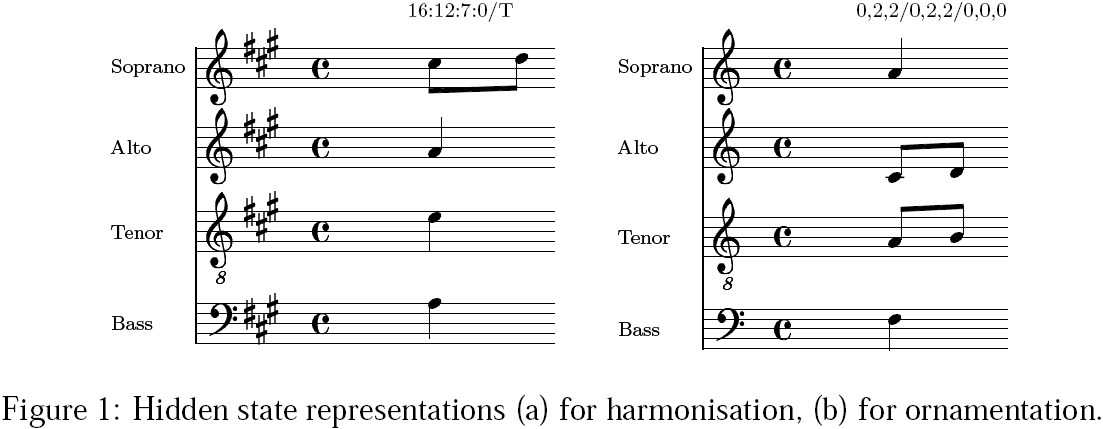
\includegraphics[width=8cm]{allan}}

}

%%%%%%%%%%%%%%%%%%%%%%%%%%%%%%%%%%%%%%%%%%%%%%%%%%%%%%%%%%%%%%%%%%%%%%%%%%%%%%%%

\slide{HMM example: Learning Bach}{

\item results: {\small\url{http://www.anc.inf.ed.ac.uk/demos/hmmbach/}}

~

\centerline{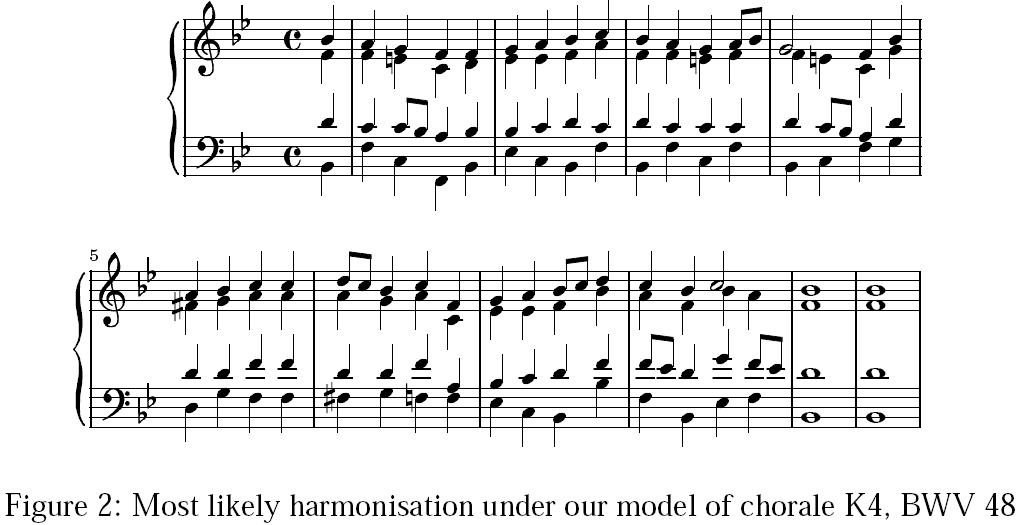
\includegraphics[width=8cm]{allan2}}

~

\item See also work by Gerhard
Widmer \url{http://www.cp.jku.at/people/widmer/}

}

%%%%%%%%%%%%%%%%%%%%%%%%%%%%%%%%%%%%%%%%%%%%%%%%%%%%%%%%%%%%%%%%%%%%%%%%%%%%%%%%

\slide{Dynamic Bayesian Networks}{\label{lastpage}

-- Arbitrary BNs in each time slide

-- Special case: MDPs, speech, etc

}

%%%%%%%%%%%%%%%%%%%%%%%%%%%%%%%%%%%%%%%%%%%%%%%%%%%%%%%%%%%%%%%%%%%%%%%%%%%%%%%%

\slidesfoot

\providecommand{\slides}{
  \newcommand{\slideshead}{
  \newcommand{\thepage}{\arabic{mypage}}
  %beamer
%  \documentclass[t,hyperref={bookmarks=true}]{beamer}
%  \geometry{papersize={171mm,96mm}}
  \documentclass[t,hyperref={bookmarks=true},aspectratio=169]{beamer}
  \setbeamersize{text margin left=5mm}
  \setbeamersize{text margin right=5mm}
  \usetheme{default}
  \usefonttheme[onlymath]{serif}
  \setbeamertemplate{navigation symbols}{}
  \setbeamertemplate{itemize items}{{\color{black}$\bullet$}}

  \newwrite\keyfile

  %\usepackage{palatino}
  \stdpackages
  %\usepackage{tikz} \usetikzlibrary {shapes.geometric} 
  \usepackage{multimedia}
  \usepackage[utf8]{inputenc}

  \hypersetup{
    colorlinks,
    linkcolor={blue!80!black},
    citecolor={blue!80!black},
    urlcolor={blue!80!black}
  }

  %%% geometry/spacing issues
  %\renewcommand{\baselinestretch}{1.1}
  \renewcommand{\arraystretch}{1.2}
  \columnsep 0mm

  \columnseprule 0pt
  \parindent 0ex
  \parskip 0ex
  %\setlength{\itemparsep}{3ex}
  %\renewcommand{\labelitemi}{\rule[3pt]{10pt}{10pt}~}
  %\renewcommand{\labelenumi}{\textbf{(\arabic{enumi})}}
  \setbeamertemplate{enumerate item}{(\roman{enumi})}
  \newcommand{\headerfont}{\helvetica{14}{1.5}{b}{n}}
  \newcommand{\slidefont} {\helvetica{11}{1.4}{m}{n}}
  %\newcommand{\codefont} {\helvetica{8}{1.2}{m}{n}}
  \newcommand{\urlfont} {\fontsize{6}{1.1}\selectfont}
  \renewcommand{\small} {\helvetica{10}{1.4}{m}{n}}
  \renewcommand{\tiny} {\helvetica{8}{1.3}{m}{n}}
  \newcommand{\ttiny} {\helvetica{7}{1.3}{m}{n}}

  %%% count pages properly and put the page number in bottom right
  %
  \newcounter{mypage}
  \newcommand{\incpage}{\addtocounter{mypage}{1}\setcounter{page}{\arabic{mypage}}}
  \setcounter{mypage}{0}
  \resetcounteronoverlays{page}

  \pagestyle{fancy}
  %\setlength{\headsep}{10mm}
  %\addtolength{\footheight}{15mm}
  \renewcommand{\headrulewidth}{0pt} %1pt}
  \renewcommand{\footrulewidth}{0pt} %.5pt}
  \cfoot{}
  \rhead{}
  \lhead{}
  %% \lfoot{\vspace*{-3mm}\hspace*{-3mm}\helvetica{5}{1.3}{m}{n}{\texttt{github.com/MarcToussaint/AI-lectures}}}
\lfoot{}
%  \rfoot{{\tiny\textsf{AI -- \topic -- \subtopic -- \arabic{mypage}/\pageref{lastpage}}}}
  %\lfoot{\raisebox{5mm}{\tiny\textsf{\slideauthor}}}
  %\rfoot{\raisebox{5mm}{\tiny\textsf{\slidevenue{} -- \arabic{mypage}/\pageref{lastpage}}}}
  %\rfoot{~\anchor{30,12}{\tiny\textsf{\thepage/\pageref{lastpage}}}}
  %\lfoot{\small\textsf{Marc Toussaint}}
  \rfoot{\vspace*{-4.5mm}{\tiny\textsf{\color{gray}\topic\ -- \subtopic\ -- \arabic{mypage}/\pageref{lastpage}}}\hspace*{-4mm}}
%  \rfoot{\vspace*{-4.5mm}{\tiny\textsf{\color{gray}\topic\ -- \arabic{mypage}/\pageref{lastpage}}}\hspace*{-4mm}}
%  \rfoot{~\anchor{-10,12}{\tiny\textsf{\color{gray}\topic\ --  \arabic{mypage}/\pageref{lastpage}}}}
  \lfoot{\vspace*{-4.5mm}{\hspace*{-4mm}\includegraphics[height=4mm]{LIS-26-text-long}}}

  \definecolor{grey}{rgb}{.8,.8,.8}
  \definecolor{head}{rgb}{.85,.9,.9}
%  \definecolor{blue}{rgb}{.0,.0,.5}
%  \definecolor{green}{rgb}{.0,.5,.0}
  \definecolor{red}{rgb}{.8,.0,.0}
  \definecolor{citcol}{gray}{.6}
  \newcommand{\inverted}{
    \definecolor{main}{rgb}{1,1,1}
    \color{main}
    \pagecolor[rgb]{.3,.3,.3}
  }
  \input{../latex/macros}

  \graphicspath{{pics/}{../pics/}{pics-local/}}
}

\newcommand{\slidestitle}{
  \title{\course \topic}
  \author{Marc Toussaint}
  \institute{Learning \& Intelligent Systems Lab, TU Berlin}

  \begin{document}


  %% title slide!
  \slide{}{
    \thispagestyle{empty}

    \twocol{.35}{.55}{
      %\vspace*{-5mm}%
      \hspace*{-5mm}%
      \includegraphics[width=1.\columnwidth]{\coursepicture}
    }{\center

      \textbf{\fontsize{17}{20}\selectfont \course}

      ~

      %Lecture
      \topic\\

      \vspace{1cm}

      {\tiny~\emph{\keywords}~\\}

      \vspace{1cm}

      \teacher
      
      Technical University of Berlin

      \coursedate

      ~

    }
  }
}

\newcommand{\slide}[2]{
  \slidefont
  \incpage\begin{frame}
  \addcontentsline{toc}{section}{#1}
  \vfill
  {\headerfont #1} \vspace*{-2ex}
  \begin{itemize}\item[]~\\
    #2
  \end{itemize}
  \vfill
  \end{frame}
}

% use \begin{frame}[fragile] around slidecore!
\newenvironment{slidecore}[1]{
  \slidefont\incpage
  \addcontentsline{toc}{section}{#1}
  \vfill
  {\headerfont #1} \vspace*{-2ex}
  \begin{itemize}\item[]~\\
}{
  \end{itemize}
  \vfill
}

\newcommand{\titleslide}[4][Marc Toussaint]{
  \newcommand{\slideauthor}{#1}
  \newcommand{\slidevenue}{#3}
  \slidefont
  \incpage
  \begin{frame}
  \begin{center}
    \vspace*{15mm}

    {\headerfont #2\\}
        
    \vspace*{10mm}

    #1 \\

    \vspace*{5mm}

    {\small
      Learning \& Intelligent Systems Lab, TU Berlin\\
%      Science of Intelligence Cluster of Excellence, Berlin\\
      Max Planck Fellow, Institute for Intelligent Systems\\ %Physical Reasoning \& Manipulation Lab -- 
%      MIT CSAIL\\
%      mtoussai@mit.edu,~ marc.toussaint@informatik.uni-stuttgart.de

      \vspace*{10mm}

      \emph{#3}
    }

    \vspace*{0mm}

    %\includegraphics[scale=.1]{pics/eushield-fullcolour}

  \end{center}
  \begin{itemize}\item[]~\\
    #4
  \end{itemize}
  \end{frame}
}

\newcommand{\titleslideempty}[2]{
  \slidefont
  \incpage
  \begin{frame}
  \begin{center}
    \vspace*{15mm}

    {\headerfont #1\\}
        
    %% \vspace*{5mm}

    %% {\small\emph{#2}} \\

  \end{center}
  \begin{itemize}\item[]~\\
    #2
  \end{itemize}
  \end{frame}
}

\providecommand{\key}[1]{
  \addtocounter{mypage}{1}
% \immediate\write\keyfile{#1}
  \addtocontents{toc}{\hyperref[key:#1]{#1 (\arabic{mypage})}}
%  \phantomsection\label{key:#1}
%  \index{#1@{\hyperref[key:#1]{#1 (\arabic{mysec}:\arabic{mypage})}}|phantom}
  \addtocounter{mypage}{-1}
}

\providecommand{\course}{}

\providecommand{\subtopic}{}

\providecommand{\sublecture}[2]{
  \renewcommand{\subtopic}{#1}
  \slide{#1}{#2}
}

\providecommand{\sublectureHide}[2]{
  \renewcommand{\subtopic}{#1}
}

\providecommand{\story}[1]{
~

Motivation: {\tiny #1}\clearpage
}

\newenvironment{items}[1][9]{
\par\setlength{\unitlength}{1pt}\fontsize{#1}{#1}\linespread{1.2}\selectfont
\begin{list}{--}{\leftmargin4ex \rightmargin0ex \labelsep1ex \labelwidth2ex
\topsep.7ex \parsep0ex \itemsep3pt}
}{
\end{list}
}

\newenvironment{itemS}[1][4ex]{
\par
\tiny
\begin{list}{--}{\leftmargin#1 \rightmargin0ex \labelsep1ex
  \labelwidth2ex \topsep0pt \parsep0ex \itemsep2pt}
}{
\end{list}
}

\providecommand{\slidesfoot}{
  \end{document}
}


  \slideshead
  \lecturetitleslide
}

\providecommand{\exercises}{
  \newcommand{\exerciseshead}{
  \documentclass[10pt,fleqn]{article}
  \stdpackages
\usepackage[utf8]{inputenc}

  \definecolor{bluecol}{rgb}{0,0,.5}
  \definecolor{greencol}{rgb}{0,.4,0}
  \definecolor{shadecolor}{gray}{0.9}
  \usepackage[
    %    pdftex%,
    %%    letterpaper,
    %    bookmarks,
    %    bookmarksnumbered,
    colorlinks,
    urlcolor=bluecol,
    citecolor=black,
    linkcolor=bluecol,
    %    pagecolor=bluecol,
    pdfborder={0 0 0},
    %pdfborderstyle={/S/U/W 1},
    %%    backref,     %link from bibliography back to sections
    %%    pagebackref, %link from bibliography back to pages
    %%    pdfstartview=FitH, %fitwidth instead of fit window
    pdfpagemode=UseNone, %UseOutlines, %bookmarks are displayed by acrobat
    pdftitle={\course},
    pdfauthor={Marc Toussaint},
    pdfkeywords={}
  ]{hyperref}
  \DeclareGraphicsExtensions{.pdf,.png,.jpg,.eps}

  \renewcommand{\r}{\varrho}
  \renewcommand{\l}{\lambda}
  \renewcommand{\L}{\Lambda}
  \renewcommand{\b}{\beta}
  \renewcommand{\d}{\delta}
  \renewcommand{\k}{\kappa}
  \renewcommand{\t}{\theta}
  \renewcommand{\O}{\Omega}
  \renewcommand{\o}{\omega}
  \renewcommand{\SS}{{\cal S}}
  \renewcommand{\=}{\!=\!}
  %\renewcommand{\boldsymbol}{}
  %\renewcommand{\Chapter}{\chapter}
  %\renewcommand{\Subsection}{\subsection}

  \renewcommand{\baselinestretch}{1.1}
  \geometry{a4paper,headsep=7mm,hdivide={15mm,*,15mm},vdivide={20mm,*,15mm}}

  \fancyhead[L]{\thetitle, \textit{\teacher}---\coursedate}
  \fancyhead[R]{\thepage}
  \fancyhead[C]{}
  \fancyfoot{}
  \pagestyle{fancy}

  \renewcommand{\labelenumi}{{\alph{enumi})}}

  \parindent 0pt
  \parskip 0.5ex

  \newcommand{\codefont}{\helvetica{8}{1.2}{m}{n}}
  \newcommand{\urlfont} {\fontsize{6}{1.1}\selectfont}
  \newcommand{\ttiny} {\helvetica{7}{1.3}{m}{n}}

  \input{../latex/macros}

  \DefineShortVerb{\@}

  \usepackage{comment}
  \specialcomment{solution}{
    \small
    \begin{shaded}
  }{
    \end{shaded}
  }
  
  \renewcommand{\hat}{\widehat}
  \newcommand{\bbg}{{\bar{\bar g}}}
  \graphicspath{{pics/}{../pics/}}

  \mytitle{\course\\\exnum}
  \myauthor{\teacher\\ \small\addressTUB}
  \date{\coursedate}
}

%%%%%%%%%%%%%%%%%%%%%%%%%%%%%%%%%%%%%%%%%%%%%%%%%%%%%%%%%%%%%%%%%%%%%%%%%%%%%%%%

\newcommand{\exercisestitle}{  
  \begin{document}
  \maketitle
}

\newcommand{\exsection}[1]{\section{#1}}

\newcommand{\exsubsection}[1]{\subsection{#1}}

\newcommand{\exerfoot}{
  \end{document}
}

\newenvironment{items}[1][9]{
  \par\setlength{\unitlength}{1pt}\fontsize{#1}{#1}\linespread{1.2}\selectfont
  \begin{list}{--}{\leftmargin4ex \rightmargin0ex \labelsep1ex \labelwidth2ex
      \topsep0pt \parsep0ex \itemsep3pt}
}{
  \end{list}
}

  \exerciseshead
}

\providecommand{\script}{
  \newcommand{\scripthead}{
  \documentclass[9pt,fleqn,twoside]{article}
  \stdpackages

  \usepackage{makeidx}
  \makeindex

  \usepackage{thmtools}
  \definecolor{shadecolor}{gray}{0.85}
  \declaretheoremstyle[
    %headfont=\normalfont\bfseries,
    %notefont=\mdseries, notebraces={(}{)},
    %bodyfont=\normalfont,
    %postheadspace=0.5em,
    %spaceabove=6pt,
    mdframed={
      %  skipabove=8pt,
      %  skipbelow=6pt,
      hidealllines=true,
      backgroundcolor={shadecolor},
      innertopmargin=8pt,
      %  innerleftmargin=3pt,
      %  innerrightmargin=3pt
    }
  ]{shaded}
  \declaretheorem[style=shaded,within=section,name=Definition]{myDefinition}
  \declaretheorem[style=shaded,within=section,name=Theorem]{myTheorem}
  \declaretheorem[style=shaded,within=section,name=Identities]{Identities}
  \declaretheorem[style=shaded,within=section,name=Example]{myExample}

  \definecolor{grey}{rgb}{.8,.8,.8}
  \definecolor{bluecol}{rgb}{0,0,.5}
  \definecolor{greencol}{rgb}{0,.4,0}
  \definecolor{shadecolor}{gray}{0.9}
  \definecolor{citcol}{rgb}{.4,.4,.4}
  \usepackage[
    %    pdftex%,
    %%    letterpaper,
    %bookmarks,
    bookmarksnumbered,
    colorlinks,
    urlcolor=bluecol,
    citecolor=black,
    linkcolor=bluecol,
    %    pagecolor=bluecol,
    pdfborder={0 0 0},
    %pdfborderstyle={/S/U/W 1},
    %%    backref,     %link from bibliography back to sections
    %%    pagebackref, %link from bibliography back to pages
    %%    pdfstartview=FitH, %fitwidth instead of fit window
    pdfpagemode=UseOutlines, %bookmarks are displayed by acrobat
    pdftitle={\course},
    pdfauthor={Marc Toussaint},
    pdfkeywords={}
  ]{hyperref}
  \DeclareGraphicsExtensions{.pdf,.png,.jpg,.eps}

  %\usepackage{multirow}
  \usepackage{multimedia}
  %\usepackage{marginnote}
  %\setbeamercolor{background canvas}{bg=}

  \usepackage[round]{natbib}
  \bibliographystyle{abbrvnat}

  \renewcommand{\r}{\varrho}
  \renewcommand{\l}{\lambda}
  \renewcommand{\L}{\Lambda}
  \renewcommand{\b}{\beta}
  \renewcommand{\d}{\delta}
  \renewcommand{\k}{\kappa}
  \renewcommand{\t}{\theta}
  \renewcommand{\O}{\Omega}
  \renewcommand{\o}{\omega}
  \renewcommand{\SS}{{\cal S}}
  \renewcommand{\=}{\!=\!}
  %\renewcommand{\boldsymbol}{}
  %\renewcommand{\Chapter}{\chapter}
  %\renewcommand{\Subsection}{\subsection}

  \renewcommand{\baselinestretch}{1.0}
  \geometry{a5paper,headsep=6mm,hdivide={10mm,*,10mm},vdivide={13mm,*,7mm}}

  \fancyhead[OL,ER]{\course, \textit{Marc Toussaint}}
  \fancyhead[OR,EL]{\thepage}
  \fancyhead[C]{}
  \fancyfoot{}
  \pagestyle{fancy}

  \renewcommand{\labelenumi}{{(\roman{enumi})}}
  \renewcommand{\theenumi}{(\roman{enumi})} %for ref
  \parindent 0pt
  \parskip .5pc

  \columnsep 6ex

  \renewcommand{\familydefault}{\sfdefault}

  \newcommand{\headerfont}{\large}%helvetica{12}{1}{b}{n}}
  \newcommand{\slidefont} {}%\helvetica{9}{1.3}{m}{n}}
  \newcommand{\storyfont} {}
  %  \renewcommand{\small}   {\helvetica{8}{1.2}{m}{n}}
  \renewcommand{\tiny}    {\footnotesize}%helvetica{7}{1.1}{m}{n}}
  \newcommand{\ttiny} {\footnotesize}%fontsize{7}{7}\selectfont}
%  \newcommand{\codefont}{\fontsize{6}{6}\selectfont}%helvetica{8}{1.2}{m}{n}}
  \newcommand{\codefont} {\helvetica{8}{1.2}{m}{n}}

  \input{../latex/macros}

  \usepackage{comment}
  \specialcomment{solution}{
    \small
    \begin{shaded}
  }{
    \end{shaded}
  }

  \graphicspath{{pics/}{../latex/pics/}}

  \mytitle{\course\\Lecture Script}
  \myauthor{Marc Toussaint}
  \date{\coursedate}
}

%%%%%%%%%%%%%%%%%%%%%%%%%%%%%%%%%%%%%%%%%%%%%%%%%%%%%%%%%%%%%%%%%%%%%%%%%%%%%%%%

\newcommand{\scripttitle}{
  \begin{document}
  \maketitle
  %\anchor{100,10}{\includegraphics[width=4cm]{optim}}
%  \vspace*{1cm}

  \emph{This is a direct concatenation and reformatting of all lecture
    slides and exercises from this course, including indexing to help
    prepare for exams.}

  {\tableofcontents}
}

%%%%%%%%%%%%%%%%%%%%%%%%%%%%%%%%%%%%%%%%%%%%%%%%%%%%%%%%%%%%%%%%%%%%%%%%%%%%%%%%

\newcounter{mypage}
\setcounter{mypage}{0}
\newcommand{\incpage}{\addtocounter{mypage}{1}}

\newcommand{\subtopic}{}
\newcommand{\pause}{}
\newcommand{\only}[1]{#1}

\renewcommand{\slides}[1][]{
  %  \clearpage
  \subsection{\topic}
  \index{\topic}
  {\small #1}
  \setcounter{mypage}{0}
  \smallskip\nopagebreak\hrule\medskip
}

\newcommand{\slidesfoot}{
  \bigskip
}

\newcommand{\sublecture}[2]{
  \index{#1}
}

\newcommand{\key}[1]{
  \phantomsection\addcontentsline{toc}{subsubsection}{#1}
  %\subsubsection{#1}
  \index{#1}
}

\providecommand{\defn}[1]{%
  \textbf{#1}\index{#1}%
}

\newenvironment{slidecore}[1]{
  \incpage
  \subsubsection*{#1}%{\headerfont\noindent\textbf{#1}\\}%
  \vspace{-6ex}%
  \begin{list}{$\bullet$}{\leftmargin4ex \rightmargin0ex \labelsep1ex
    \labelwidth2ex \partopsep0ex \topsep0ex \parsep.5ex \parskip0ex \itemsep0pt}\item[]~\\\nopagebreak%
}{
  \end{list}\nopagebreak%
  {\hfill\tiny \textsf{\arabic{section}.\arabic{subsection}:\arabic{mypage}}}\nopagebreak%
  \smallskip\nopagebreak\hrule
}

\newcommand{\slide}[2]{
  \begin{slidecore}{#1}
    #2
  \end{slidecore}
}

\renewcommand{\exercises}{}
\newcommand{\exercisestitle}{}
\newcommand{\exsection}[1]{\subsubsection{#1}}
\newcommand{\exerfoot}{\bigskip}

\newcommand{\story}[1]{
  \subsection*{Motivation \& Outline}
  {\storyfont\sf #1}
  \medskip\nopagebreak\hrule
}

\newcounter{savedsection}
\newcommand{\subappendix}{\setcounter{savedsection}{\arabic{section}}\appendix}
\newcommand{\noappendix}{
  \setcounter{section}{\arabic{savedsection}}% restore section number
  \setcounter{subsection}{0}% reset section counter
%  \gdef\@chapapp{\sectionname}% reset section name
  \renewcommand{\thesection}{\arabic{section}}% make section numbers arabic
}

\newenvironment{items}[1][9]{
\par\setlength{\unitlength}{1pt}\fontsize{#1}{#1}\linespread{1.2}\selectfont
\begin{list}{--}{\leftmargin4ex \rightmargin0ex \labelsep1ex \labelwidth2ex
\topsep0pt \parsep0ex \itemsep3pt}
}{
\end{list}
}

\newcommand{\Def}[1]{%
\textbf{#1}\index{#1}}%\marginnote{#1}}

  \scripthead
}

\providecommand{\note}{
  \providecommand{\notehead}[2]{
  \documentclass[#1,fleqn,twoside]{article}
  \stdpackages
  \renewcommand{\labelenumi}{{(\roman{enumi})}}
  \renewcommand{\theenumi}{(\roman{enumi})} %for ref

  \renewcommand{\baselinestretch}{#2}
  \renewcommand{\arraystretch}{1.2}
  \renewcommand{\topfraction}{1}
  \renewcommand{\bottomfraction}{1}
  \renewcommand{\textfraction}{0}
  \columnsep 5ex
  \parindent 3ex
  \parskip 1ex

  % Lists and paragraphs
  \parindent 0pt
  \topsep 4pt plus 1pt minus 2pt
  \partopsep 1pt plus 0.5pt minus 0.5pt
  \itemsep 2pt plus 1pt minus 0.5pt
  \parsep 2pt plus 1pt minus 0.5pt
  \parskip .5pc %add _in_ {thebibliography} environment in *.bbl

  \setcounter{tocdepth}{3}
  \setcounter{secnumdepth}{3}

  \geometry{a4paper,hdivide={25mm,*,25mm},vdivide={25mm,*,25mm}}

  \renewcommand{\headrulewidth}{.0pt}\renewcommand{\footrulewidth}{.0pt}\cfoot{}
  \fancyhead[OL,EC]{\it\theauthor---\today}
  \fancyhead[ER]{\leftmark}
  \fancyhead[OR,EL]{\thepage}
  \fancyfoot[EL,OR]{}
  \setlength{\headsep}{10mm}
  %\fancyhead[OL]{\rightmark}
  %\fancyfoot[EL,OR]{}


  %  \usepackage{palatino}

  \newcommand{\codefont}{\helvetica{8}{1.2}{m}{n}}

  \renewenvironment{abstract}{
    \vspace*{5ex}\begin{list}{}{
      \leftmargin3ex
      \rightmargin3ex
      \topsep-\parskip}\item[]
     \hrule\vspace{1.5ex}{\bf Abstract.~}\small}
    {\vspace{2ex}\hrule\end{list}\vspace{5ex}}
    
  \newenvironment{keyword}
    {\par{\it Keywords:~}}
    {}

  \def\makemytitle{%
    \thispagestyle{empty}
    \begin{list}{}{\leftmargin3ex \rightmargin3ex \topsep0ex \parsep0ex}\item[]
      \begin{center}
        {\fontsize{18}{25}\selectfont{\thetitle\\}}\vspace{5ex}

        {\fontsize{14}{16}\selectfont{\theauthor\\}}\vspace{1ex}

        {\footnotesize{\sl \addressFUB}\\ \emailBerlin}

        {\footnotesize \today}

        \vspace{1ex}
        {\small \published}
      \end{center}
    \end{list}
    \renewcommand{\maketitle}{\chapter{\thetitle}}
  }

  \input{../latex/macros}
  \pdflatex

  \graphicspath{{pics/}{../pics/}{pics-local/}}

  \myauthor{Marc Toussaint}
  \date{\today}
}

%%%%%%%%%%%%%%%%%%%%%%%%%%%%%%%%%%%%%%%%%%%%%%%%%%%%%%%%%%%%%%%%%%%%%%%%%%%%%%%%

\newcommand{\notetitle}{
  \begin{document}
  \thispagestyle{empty}
    
  \maketitle

}

\newenvironment{items}[1][9]{
\par\setlength{\unitlength}{1pt}\fontsize{#1}{#1}\linespread{1.2}\selectfont
\begin{list}{--}{\leftmargin4ex \rightmargin0ex \labelsep1ex \labelwidth2ex
\topsep0pt \parsep0ex \itemsep3pt}
}{
\end{list}
}

  \notehead{10}{1.1}
}

\providecommand{\course}{NO COURSE}
\providecommand{\coursepicture}{NO PICTURE}
\providecommand{\coursedate}{NO DATE}
\providecommand{\topic}{NO TOPIC}
\providecommand{\keywords}{NO KEYWORDS}
\providecommand{\exnum}{NO NUMBER}
\providecommand{\teacher}{Marc Toussaint}

\providecommand{\stdpackages}{
  \usepackage{amsmath}
  \usepackage{amssymb}
  \usepackage{amsfonts}
  \allowdisplaybreaks
  \usepackage{amsthm}
  \usepackage{eucal}
  \usepackage{graphicx}
  \usepackage{color}
  \usepackage{geometry}
  \usepackage{framed}
%  \usecolor{xcolor}
  \definecolor{shadecolor}{gray}{0.9}
  \setlength{\FrameSep}{3pt}
  \usepackage{fancyvrb}
  \fvset{numbers=none,xleftmargin=5ex}

  \usepackage{pdfpages}

  \usepackage{multicol} 
  \usepackage{fancyhdr}
}

\providecommand{\addressUSTT}{
  Machine~Learning~\&~Robotics~lab, U~Stuttgart\\\small
  Universit{\"a}tsstra{\ss}e 38, 70569~Stuttgart, Germany
}

\providecommand{\addressTUB}{
  Learning~\&~Intelligent~Systems~Lab, TU~Berlin\\\small
  Marchstr. 23, 10587 Berlin, Germany
}


\renewcommand{\course}{Artificial Intelligence}
\renewcommand{\coursepicture}{course_ai}
\renewcommand{\coursedate}{Winter 2019}
\renewcommand{\topic}{Propositional Logic}
\renewcommand{\keywords}{}

\slides

%[(slides based on Stuart Russell's AI course)]

\slidestitle

%%%%%%%%%%%%%%%%%%%%%%%%%%%%%%%%%%%%%%%%%%%%%%%%%%%%%%%%%%%%%%%%%%%%%%%%%%%%%%%%

\story{

Most students will have learnt about propositional logic their first
classes. It represents the simplest and most basic kind of logic.
The main motivation to teach it really is as a precursor of
first-order logic (FOL), which is covered in the next lecture. The intro of
the next lecture motivates FOL in detail. The main point is that in
recent years there were important developments that unified FOL
methods with probabilistic reasoning and learning methods, which
really allows to tackle novel problems.

In this lecture we go quickly over the syntax and semantics of
propositional logic. Then we cover the basic methods for logic
inference: fwd \& bwd chaining, as well as resolution.



}

%%%%%%%%%%%%%%%%%%%%%%%%%%%%%%%%%%%%%%%%%%%%%%%%%%%%%%%%%%%%%%%%%%%%%%%%%%%%%%%%

\sublecture{Syntax \& Semantics}{}

%%%%%%%%%%%%%%%%%%%%%%%%%%%%%%%%%%%%%%%%%%%%%%%%%%%%%%%%%%%%%%%%%%%%%%

\slide{Outline}{

\item Example: Knowledge-based agents \& Wumpus world


\item Logic in general---models and entailment

\item Propositional (Boolean) logic

\item Equivalence, validity, satisfiability

\item Inference rules and theorem proving\\
 -- forward chaining\\
 -- backward chaining\\
 -- resolution

%\item Model checking
%
%\item Propositional knowledge-based agents
%
%\item Boolean circuit agents

}

%%%%%%%%%%%%%%%%%%%%%%%%%%%%%%%%%%%%%%%%%%%%%%%%%%%%%%%%%%%%%%%%%%%%%%

\key{Knowledge base: Definition}
\slide{Knowledge bases}{

~

\show[.6]{markov}

~

\item An agent maintains a knowledge base

%% \show[0.8]
%% \show{russell/kbs.pdf}

~

\defn{Knowledge base} = \defn{set of sentences} of a \emph{formal} language

%% ~

%% \defn{Declarative} approach to building an agent (or other system):\\
%%    \defprog{Tell} it what it needs to know

%% Then it can \defprog{Ask} itself what to do---answers should follow from the KB

%% Agents can be viewed at the \defn{knowledge level}\\
%%    i.e., \emph{what they know}, regardless of how implemented

%% Or at the \defn{implementation level}\\
%%    i.e., data structures in KB and algorithms that manipulate them

}

%%%%%%%%%%%%%%%%%%%%%%%%%%%%%%%%%%%%%%%%%%%%%%%%%%%%%%%%%%%%%%%%%%%%%%

%% \slide{A simple knowledge-based agent}{

%% \input{russell/logical-agent-algorithm}

%% The agent must be able to:\\ \quad
%% Represent states, actions, etc.\\ \quad
%% Incorporate new percepts\\ \quad
%% Update internal representations of the world\\ \quad
%% Deduce hidden properties of the world\\ \quad
%% Deduce appropriate actions

%% }

%%%%%%%%%%%%%%%%%%%%%%%%%%%%%%%%%%%%%%%%%%%%%%%%%%%%%%%%%%%%%%%%%%%%%%

\key{Wumpus World example}
\slide{Wumpus World description}{

\hspace*{-5mm}\begin{tabular}{lr}
\hbox{\begin{minipage}[b]{0.6\columnwidth}
\emph{Performance measure} \\ \quad
  gold +1000, death -1000\\ \quad
  -1 per step, -10 for using the arrow

\emph{Environment}\\ \quad
Squares adjacent to wumpus are smelly\\ \quad
Squares adjacent to pit are breezy\\ \quad
Glitter iff gold is in the same square\\ \quad
Shooting kills wumpus if you are facing it\\ \quad
The wumpus kills you if in the same square\\ \quad
Shooting uses up the only arrow\\ \quad
Grabbing picks up gold if in same square\\ \quad
Releasing drops the gold in same square
\end{minipage}}
&
\showh[0.34]{russell/wumpus-world.pdf}
\end{tabular}

\emph{Actuators} Left turn, Right turn,\\
    Forward, Grab, Release, Shoot, Climb

\emph{Sensors} Breeze, Glitter, Stench, Bump, Scream



}

%%%%%%%%%%%%%%%%%%%%%%%%%%%%%%%%%%%%%%%%%%%%%%%%%%%%%%%%%%%%%%%%%%%%%%
%% \slide{Wumpus world characterization}{

%% \emph{Observable} 

%% }

%% %%%%%%%%%%%%%%%%%%%%%%%%%%%%%%%%%%%%%%%%%%%%%%%%%%%%%%%%%%%%%%%%%%%%%%
%% \slide{Wumpus world characterization}{

%% \emph{Observable} No---only \emph{local} perception

%% \emph{Deterministic} 

%% }

%% %%%%%%%%%%%%%%%%%%%%%%%%%%%%%%%%%%%%%%%%%%%%%%%%%%%%%%%%%%%%%%%%%%%%%%
%% \slide{Wumpus world characterization}{

%% \emph{Observable} No---only \emph{local} perception

%% \emph{Deterministic} Yes---outcomes exactly specified

%% %% \emph{Episodic} 

%% %% }

%% %%%%%%%%%%%%%%%%%%%%%%%%%%%%%%%%%%%%%%%%%%%%%%%%%%%%%%%%%%%%%%%%%%%%%%
%% %% \slide{Wumpus world characterization}{

%% %% \emph{Observable} No---only \emph{local} perception

%% %% \emph{Deterministic} Yes---outcomes exactly specified

%% %% \emph{Episodic} No---sequential at the level of actions

%% %% \emph{Static}  

%% }

%% %%%%%%%%%%%%%%%%%%%%%%%%%%%%%%%%%%%%%%%%%%%%%%%%%%%%%%%%%%%%%%%%%%%%%%
%% \slide{Wumpus world characterization}{

%% \emph{Observable} No---only \emph{local} perception

%% \emph{Deterministic} Yes---outcomes exactly specified

%% %\emph{Episodic} No---sequential at the level of actions

%% \emph{Static}  Yes---Wumpus and Pits do not move

%% \emph{Discrete} 

%% }

%% %%%%%%%%%%%%%%%%%%%%%%%%%%%%%%%%%%%%%%%%%%%%%%%%%%%%%%%%%%%%%%%%%%%%%%
%% \slide{Wumpus world characterization}{

%% \emph{Observable} No---only \emph{local} perception

%% \emph{Deterministic} Yes---outcomes exactly specified

%% %\emph{Episodic} No---sequential at the level of actions

%% \emph{Static}  Yes---Wumpus and Pits do not move

%% \emph{Discrete} Yes

%% \emph{Single-agent} 

%% }

%% %%%%%%%%%%%%%%%%%%%%%%%%%%%%%%%%%%%%%%%%%%%%%%%%%%%%%%%%%%%%%%%%%%%%%%
%% \slide{Wumpus world characterization}{

%% \emph{Observable} No---only \emph{local} perception

%% \emph{Deterministic} Yes---outcomes exactly specified

%% %\emph{Episodic} No---sequential at the level of actions

%% \emph{Static}  Yes---Wumpus and Pits do not move

%% \emph{Discrete} Yes

%% \emph{Single-agent} Yes---Wumpus is essentially a natural feature




%% }

%%%%%%%%%%%%%%%%%%%%%%%%%%%%%%%%%%%%%%%%%%%%%%%%%%%%%%%%%%%%%%%%%%%%%%
\slide{Exploring a wumpus world}{

\vspace*{0.4in}

\only<1>{\show[0.35]{russell/wumpus-seq0c}}
\only<2>{\show[0.35]{russell/wumpus-seq1c}}
\only<3>{\show[0.35]{russell/wumpus-seq2c}}
\only<4>{\show[0.35]{russell/wumpus-seq3c}}
\only<5>{\show[0.35]{russell/wumpus-seq4c}}
\only<6>{\show[0.35]{russell/wumpus-seq5c}}
\only<7>{\show[0.35]{russell/wumpus-seq6c}}
\only<8>{\show[0.35]{russell/wumpus-seq7c}}


}

%%%%%%%%%%%%%%%%%%%%%%%%%%%%%%%%%%%%%%%%%%%%%%%%%%%%%%%%%%%%%%%%%%%%%%
\slide{Other tight spots}{

\twocol[.05]{.4}{.5}{
\show[.5]{russell/wumpus-bb.pdf}
}{
Breeze in (1,2) and (2,1)\\ \quad
$\implies$ no safe actions

Assuming pits uniformly distributed,\\
(2,2) has pit w/ prob 0.86, vs.~0.31
}

~

~

\twocol[.15]{.3}{.5}{
\show[.5]{russell/wumpus-s.pdf}
}{
Smell in (1,1) $\implies$ cannot move

Can use a strategy of \defn{coercion}:\\ \quad
  shoot straight ahead\\ \quad
  wumpus was there $\implies$ dead $\implies$ safe\\ \quad
  wumpus wasn't there $\implies$ safe
}

}

%%%%%%%%%%%%%%%%%%%%%%%%%%%%%%%%%%%%%%%%%%%%%%%%%%%%%%%%%%%%%%%%%%%%%%

\key{Logic: Definition, Syntax, Semantics}
\slide{Logic in general}{

\item A \defn{Logic} is a formal languages for representing information
   such that conclusions can be drawn

\item The \defn{Syntax} defines the sentences in the language

\item The \defn{Semantics} defines the ``meaning'' of sentences;
   i.e., define \defn{truth} of a sentence in a world

~

E.g., the language of arithmetic

$x+2 \geq y$ is a sentence; $x2+y>{}$ is not a sentence

$x+2 \geq y$ is true iff the number $x+2$ is no less
than the number $y$

$x+2 \geq y$ is true in a world where $x = 7,\ y = 1$\\
$x+2 \geq y$ is false in a world where $x = 0,\ y = 6$

}

%%%%%%%%%%%%%%%%%%%%%%%%%%%%%%%%%%%%%%%%%%%%%%%%%%%%%%%%%%%%%%%%%%%%%%%%%%%%%%%%

\slide{Notions in general logic}{

\item A \defn{logic} is a language, elements $\a$ are \defn{sentences}

\item A \defn{model} $m$ is a world/state description that allows us to evaluate $\a(m)\in\{\textsf{true},\textsf{false}\}$
uniquely for any sentence $\a$

We define $M(\a)=\{m:\a(m)=\textsf{true}\}$ as the models for
which $\a$ holds

\item \defn{Entailment} $\a \models \b$:~ $M(\a) \subseteq M(\b)$,
~{\color{gray}``$\forall_m:~ \a(m) \implies \b(m)$''} ~ {(Folgerung)}

\item \defn{Equivalence}
$\alpha\equiv\beta$:~ iff ($\alpha\models\beta$ and
$\beta\models\alpha$)

\item A \defn{KB} is a set (=conjunction) of sentences

\item An \defn{inference} procedure $i$ can infer $\a$ from KB: $KB\vdash_i\alpha$

\item \defn{soundness} of $i$:~ $KB\vdash_i\alpha$ implies $KB\models\alpha$ ~ {(Korrektheit)}

\item \defn{completeness} of $i$:~ $KB\models\alpha$ implies $KB\vdash_i\alpha$

}

%%%%%%%%%%%%%%%%%%%%%%%%%%%%%%%%%%%%%%%%%%%%%%%%%%%%%%%%%%%%%%%%%%%%%%%%%%%%%%%%
\key{Propositional logic: Syntax}
\slide{Propositional logic: Syntax}{

\begin{tabular}{lcl}
$\langle$ sentence$\rangle$ & $\to$ & $\langle$ atomic sentence$\rangle$ $\mid$ $\langle$ complex sentence$\rangle$ \\
$\langle$ atomic sentence$\rangle$
 & $\to$ & true $\mid$ false $\mid$ $P$ $\mid$ $Q$ $\mid$ $R$ $\mid$ \dots \\
$\langle$ complex sentence$\rangle$
 & $\to$ & $\lnot$ $\langle$ sentence$\rangle$ \\
&& $\mid$ ($\langle$ sentence$\rangle$ $\land$ $\langle$ sentence$\rangle$) \\
&& $\mid$ ($\langle$ sentence$\rangle$ $\lor$ $\langle$ sentence$\rangle$) \\
&& $\mid$ ($\langle$ sentence$\rangle$ $\implies$ $\langle$ sentence$\rangle$) \\
&& $\mid$ ($\langle$ sentence$\rangle$ $\iff$ $\langle$ sentence$\rangle$) \\
\end{tabular}

}

%%%%%%%%%%%%%%%%%%%%%%%%%%%%%%%%%%%%%%%%%%%%%%%%%%%%%%%%%%%%%%%%%%%%%%

\key{Propositional logic: Semantics}
\slide{Propositional logic: Semantics}{

\item Each model specifies true/false for each proposition symbol

\begin{tabular}{lccc}
E.g. & $P_{1,2}$ & $P_{2,2}$ & $P_{3,1}$\\
     & $\textsf{true}$   &  $\textsf{true}$ &  $\textsf{false}$
\end{tabular}

(With these symbols, 8 possible models, can be enumerated automatically.)

\item Rules for evaluating truth with respect to a model $m$:

{\small \begin{tabular}{rcclcl}
$\lnot S$          & is true iff & $S$ & is false & & \\
$S_1 \land S_2$    & is true iff & $S_1$ & is true \emph{and} & $S_2$ & is true\\
$S_1 \lor S_2$     & is true iff & $S_1$ & is true \emph{or} & $S_2$ & is true\\
$S_1 \implies S_2$ & is true iff& $S_1$ & is false \emph{or} & $S_2$ & is true\\
\qquad i.e.,  & is false iff& $S_1$ & is true \emph{and} & $S_2$ & is false\\
$S_1 \iff S_2$ & is true iff& $S_1\implies S_2$ & is true \emph{and} & $S_2\implies S_1$ & is true
\end{tabular}}

\item Simple recursive process evaluates an arbitrary sentence, e.g.,\\
$\lnot P_{1,2}\land (P_{2,2}\lor P_{3,1})$ = {$\textsf{true}\land (\textsf{false} \lor \textsf{true}) = \textsf{true}\land
\textsf{true}  = \textsf{true}$}

}

%%%%%%%%%%%%%%%%%%%%%%%%%%%%%%%%%%%%%%%%%%%%%%%%%%%%%%%%%%%%%%%%%%%%%%%%%%%%%%%%
\slide{Notions in propositional logic -- summary}{

\small

\item \defn{conjunction}: $\a \land \b$, \defn{disjunction}: $\a \lor \b$, \defn{negation}: $\neg\a$

\item \defn{implication}: {$\alpha\implies \beta
~\equiv~ \lnot \alpha \lor \beta$}

\item \defn{biconditional}: $\alpha\iff \beta ~\equiv~ (\alpha\implies \beta)\land (\beta\implies \alpha)$

Note: $\models$ and $\equiv$ are statements about sentences in a logic;
$\implies$ and $\iff$ are symbols in the grammar of propositional logic

\item $\a$ \defn{valid}: true for \emph{any} model
(allgemeing{\"u}ltig). E.g., $\textsf{true}$;~ $A \lor \lnot A$;~ $A \implies A$;~ 
      $(A \land (A \implies B)) \implies B$

Note: $KB \models \alpha$ ~iff~ [$(KB \implies \alpha)$ is
valid]

\item $\a$ \defn{unsatisfiable}: true for \emph{no} model. E.g.,
$A\land \lnot A$;

Note: $KB \models \alpha$ ~iff~ [$(KB \land \lnot \alpha)$ is unsatisfiable]

\item \defn{literal}: $A$ or $\neg A$, \defn{clause}: disj.\ of literals, \defn{CNF}: conj.\ of clauses

\item \defn{Horn clause}: symbol $\mid$ (conjunction of symbols $\implies$ symbol), \defn{Horn form}: conjunction of Horn clauses

\defn{Modus Ponens} rule: complete for Horn KBs
$\frac{\alpha_1,\ldots,\alpha_n,\qquad \alpha_1\land \cdots \land \alpha_n\implies \beta}{\beta}$

\defn{Resolution} rule: complete for propositional logic in CNF,
let ``$\ell_i = \neg m_j$'':

{\cen{$\frac {\ell_1 \lor \cdots\lor \ell_k,\qquad m_1 \lor \cdots\lor m_n}
        {\ell_1 \lor \cdots\lor \ell_{i-1}\lor \ell_{i+1}\lor\cdots\lor \ell_k
        \lor m_1 \lor \cdots \lor m_{j-1}\lor m_{j+1}\lor\cdots\lor m_n}
$}}

}


%%%%%%%%%%%%%%%%%%%%%%%%%%%%%%%%%%%%%%%%%%%%%%%%%%%%%%%%%%%%%%%%%%%%%%%%%%%%%%%%

\key{Logical equivalence}
\slide{Logical equivalence}{

\item Two sentences are \defn{logically equivalent} iff true in same models:\\ \quad
$\alpha\equiv\beta$ if and only if $\alpha\models\beta$ 
and $\beta\models\alpha$

\small

\begin{align*}
(\alpha\land \beta) &\quad\equiv\quad (\beta\land \alpha) \quad\mbox{commutativity of }\land\\
(\alpha\lor \beta) &\quad\equiv\quad (\beta\lor \alpha) \quad\mbox{commutativity of }\lor\\
((\alpha\land \beta)\land \gamma) &\quad\equiv\quad (\alpha\land (\beta\land \gamma))  \quad\mbox{associativity of }\land\\
((\alpha\lor \beta)\lor \gamma) &\quad\equiv\quad (\alpha\lor (\beta\lor \gamma))  \quad\mbox{associativity of }\lor\\
\lnot(\lnot \alpha) &\quad\equiv\quad \alpha \quad\mbox{double-negation elimination}\\
(\alpha\implies \beta) &\quad\equiv\quad (\lnot \beta \implies \lnot \alpha) \quad\mbox{contraposition}\\
(\alpha\implies \beta) &\quad\equiv\quad (\lnot \alpha \lor \beta) \quad\mbox{implication elimination}\\
(\alpha\iff \beta) &\quad\equiv\quad ((\alpha\implies \beta)\land (\beta\implies \alpha)) \quad\mbox{biconditional elimination}\\
\lnot(\alpha\land \beta) &\quad\equiv\quad (\lnot \alpha \lor \lnot \beta) \quad\mbox{De Morgan}\\
\lnot(\alpha\lor \beta) &\quad\equiv\quad (\lnot \alpha \land \lnot \beta) \quad\mbox{De Morgan}\\
(\alpha\land (\beta\lor \gamma)) &\quad\equiv\quad ((\alpha\land \beta)\lor (\alpha\land \gamma))\quad\mbox{distributivity of }\land\mbox{ over }\lor\\
(\alpha\lor (\beta\land \gamma)) &\quad\equiv\quad ((\alpha\lor \beta)\land (\alpha\lor \gamma)) \quad\mbox{distributivity of }\lor\mbox{ over }\land
\end{align*}


%\hspace*{-10mm}\input{\file{tables}{logical-equivalence-table}}

}


%%%%%%%%%%%%%%%%%%%%%%%%%%%%%%%%%%%%%%%%%%%%%%%%%%%%%%%%%%%%%%%%%%%%%%
%% \key{Entailment}
%% \slide{Entailment}{

%% \defn{Entailment} means that one thing \emph{follows from} another:
%% {$$KB \models \alpha$$}

%% \item Knowledge base $KB$ entails sentence $\alpha$
%%   if and only if $\alpha$ is true in all worlds where $KB$
%%   is true

%% ~

%% E.g., the KB containing ``the Giants won'' and ``the Reds won''
%% entails ``The Giants won or the Reds won''

%% E.g., $x+y = 4$ entails  $4 = x+y$

%% \item Entailment is a relationship between sentences (i.e., \emph{syntax})
%% that is based on \emph{semantics}

%% %Note: brains process \emph{syntax} (of some sort)

%% }

%%%%%%%%%%%%%%%%%%%%%%%%%%%%%%%%%%%%%%%%%%%%%%%%%%%%%%%%%%%%%%%%%%%%%%
%% \key{Model}
%% \slide{Models}{

%% Given a logical sentence, when is its truth uniquely
%% defined in a world?

%% Logicians typically think in terms of \defn{models}, which are
%% formally structured worlds\\ (e.g.,\ full abstract description of a
%% world, configuration of all variables, world state)\\ with respect to
%% which truth can uniquely be evaluated

%% We say $m$ \emph{is a model of} a sentence $\alpha$
%% if $\alpha$ is true in $m$

%% $M(\alpha)$ is the set of all models of $\alpha$

%% Then $KB \models \alpha$ if and only if $M(KB) \subseteq M(\alpha)$

%% \twocol{.6}{.4}{
%% E.g. $KB$ = Giants won and Reds won\\
%%      $\alpha$ = Giants won
%% }{
%% \show{russell/model-inclusion.pdf}
%% }

%% }

%%%%%%%%%%%%%%%%%%%%%%%%%%%%%%%%%%%%%%%%%%%%%%%%%%%%%%%%%%%%%%%%%%%%%%

\slide{Example: Entailment in the wumpus world}{

\twocol{.6}{.4}{
Situation after detecting nothing in [1,1],\\
moving right, breeze in [2,1]

~

Consider possible models for ?s\\
assuming only pits 

~

3 Boolean choices $\implies$ 8 possible models
}{
\show{russell/wumpus-seq1c-alt.pdf}
}

}

%%%%%%%%%%%%%%%%%%%%%%%%%%%%%%%%%%%%%%%%%%%%%%%%%%%%%%%%%%%%%%%%%%%%%%
\slide{Wumpus models}{

\show[0.7]{russell/wumpus-models1.pdf}

}

%%%%%%%%%%%%%%%%%%%%%%%%%%%%%%%%%%%%%%%%%%%%%%%%%%%%%%%%%%%%%%%%%%%%%%
\slide{Wumpus models}{

\show[0.7]{russell/wumpus-models2.pdf}

$KB$ = wumpus-world rules + observations

}

%%%%%%%%%%%%%%%%%%%%%%%%%%%%%%%%%%%%%%%%%%%%%%%%%%%%%%%%%%%%%%%%%%%%%%
\slide{Wumpus models}{

\show[0.7]{russell/wumpus-models3.pdf}

$KB$ = wumpus-world rules + observations

$\alpha_1$ = ``[1,2] is safe'', $KB \models \alpha_1$, proved by \defn{model checking}


}

%%%%%%%%%%%%%%%%%%%%%%%%%%%%%%%%%%%%%%%%%%%%%%%%%%%%%%%%%%%%%%%%%%%%%%
%% \slide{Wumpus models}{

%% \show[0.7]
%% \show{russell/wumpus-models2.pdf}

%% $KB$ = wumpus-world rules + observations

%% }

%%%%%%%%%%%%%%%%%%%%%%%%%%%%%%%%%%%%%%%%%%%%%%%%%%%%%%%%%%%%%%%%%%%%%%
\slide{Wumpus models}{

\show[0.7]{russell/wumpus-models4.pdf}

$KB$ = wumpus-world rules + observations

$\alpha_2$ = ``[2,2] is safe'', $KB  \not\models \alpha_2$



}

%%%%%%%%%%%%%%%%%%%%%%%%%%%%%%%%%%%%%%%%%%%%%%%%%%%%%%%%%%%%%%%%%%%%%%

%%%%%%%%%%%%%%%%%%%%%%%%%%%%%%%%%%%%%%%%%%%%%%%%%%%%%%%%%%%%%%%%%%%%%%
%% \slide{Propositional logic: Syntax}{

%% Propositional logic is the simplest logic---illustrates basic ideas

%% The proposition symbols $P_1$, $P_2$ etc are sentences

%% If $S$ is a sentence, $\lnot S$ is a sentence (\defn{negation})

%% If $S_1$ and $S_2$ are sentences, $S_1 \land S_2$ is a sentence (\defn{conjunction})
 
%% If $S_1$ and $S_2$ are sentences, $S_1 \lor S_2$ is a sentence (\defn{disjunction})

%% If $S_1$ and $S_2$ are sentences, $S_1 \implies S_2$ is a sentence (\defn{implication})

%% If $S_1$ and $S_2$ are sentences, $S_1 \iff S_2$ is a sentence (\defn{biconditional})



%% }

%% \slide{Truth tables for connectives}{

%% \cen{\input{\file{tables}{truth-tables-table}}}

%% }

%%%%%%%%%%%%%%%%%%%%%%%%%%%%%%%%%%%%%%%%%%%%%%%%%%%%%%%%%%%%%%%%%%%%%%
%% \slide{Wumpus world sentences}{

%% Let $P_{i,j}$ be true if there is a pit in $[i,j]$.\\
%% Let $B_{i,j}$ be true if there is a breeze in $[i,j]$.
%% {\begin{eqnarray*}
%%  \lnot P_{1,1}\\
%%  \lnot B_{1,1}\\
%%  B_{2,1}
%% \end{eqnarray*}}
%% ``Pits cause breezes in adjacent squares''

%% }

%%%%%%%%%%%%%%%%%%%%%%%%%%%%%%%%%%%%%%%%%%%%%%%%%%%%%%%%%%%%%%%%%%%%%%
%% \slide{Wumpus world sentences}{

%% Let $P_{i,j}$ be true if there is a pit in $[i,j]$.\\
%% Let $B_{i,j}$ be true if there is a breeze in $[i,j]$.
%% {\begin{eqnarray*}
%%  \lnot P_{1,1}\\
%%  \lnot B_{1,1}\\
%%  B_{2,1}
%% \end{eqnarray*}}
%% ``Pits cause breezes in adjacent squares''
%% {\begin{eqnarray*}
%%  B_{1,1} &\iff& (P_{1,2} \lor P_{2,1})\\
%%  B_{2,1} &\iff& (P_{1,1} \lor P_{2,2}\lor P_{3,1})
%% \end{eqnarray*}}
%% ``A square is breezy \emph{if and only if} there is an adjacent pit''

%% }


%%%%%%%%%%%%%%%%%%%%%%%%%%%%%%%%%%%%%%%%%%%%%%%%%%%%%%%%%%%%%%%%%%%%%%%%%%%%%%%%

\sublecture{Inference Methods}{}

%%%%%%%%%%%%%%%%%%%%%%%%%%%%%%%%%%%%%%%%%%%%%%%%%%%%%%%%%%%%%%%%%%%%%%

\key{Inference}
\slide{Inference}{

\item Inference in the general sense means: Given some pieces of information
(prior, observed variabes, knowledge base) what is the implication (the implied
information, the posterior) on other things (non-observed variables, sentence)

~

\item $KB\vdash_i\alpha$ = sentence $\alpha$ can be derived from $KB$ by procedure $i$

Consequences of $KB$ are a haystack; $\alpha$ is a needle.\\
Entailment = needle in haystack; inference = finding it

\item \defn{Soundness}: $i$ is sound if\\
whenever $KB\vdash_i\alpha$, it is also true that $KB\models\alpha$

\defn{Completeness}: $i$ is complete if\\
whenever $KB\models\alpha$, it is also true that $KB\vdash_i\alpha$

~

{\tiny
Preview: we will define a logic (first-order logic) which is
expressive enough to say almost anything of interest, and for which
there exists a sound and complete inference procedure. That is, the procedure will answer any question whose answer follows
from what is known by the $KB$.

}

}

%%%%%%%%%%%%%%%%%%%%%%%%%%%%%%%%%%%%%%%%%%%%%%%%%%%%%%%%%%%%%%%%%%%%%%

\slide{Inference by enumeration}{

%\cen{\small\input{russell/wumpus-model-table}}

Enumerate rows (different assignments to symbols),\\
if {KB} is true in row, check that $\alpha$ is too


}

%%%%%%%%%%%%%%%%%%%%%%%%%%%%%%%%%%%%%%%%%%%%%%%%%%%%%%%%%%%%%%%%%%%%%%
\slide{Inference by enumeration}{

Depth-first enumeration of all models is sound and complete 

%\input{russell/tt-entails-algorithm}

$O(2^n)$ for $n$ symbols%; problem is \emph{co-NP-complete}

}


%%%%%%%%%%%%%%%%%%%%%%%%%%%%%%%%%%%%%%%%%%%%%%%%%%%%%%%%%%%%%%%%%%%%%%%%%%%%%%%%
\slide{Proof methods}{

\item Proof methods divide into (roughly) two kinds:

\item {Application of inference rules}\\ \quad
    -- Legitimate (sound) generation of new sentences from old\\ \quad
    -- \defn{Proof} = a sequence of inference rule applications\\
       Can use inference rules as operators in a standard search alg.\\ \quad
    -- Typically require translation of sentences into a \defn{normal form}

\item {Model checking}\\ \quad
    truth table enumeration (always exponential in $n$)\\ \quad
    improved backtracking, e.g., Davis--Putnam--Logemann--Loveland
    (see book)\\ \quad
    heuristic search in model space (sound but incomplete)\\
       e.g., min-conflicts-like hill-climbing algorithms




}

%%%%%%%%%%%%%%%%%%%%%%%%%%%%%%%%%%%%%%%%%%%%%%%%%%%%%%%%%%%%%%%%%%%%%%
\key{Horn Form}
\key{Modus Ponens}
\slide{Forward and backward chaining}{

\item Applicable when KB is in Horn Form

\item \defn{Horn Form} (restricted)\\
    KB = \emph{conjunction} of \emph{Horn clauses}\\ \quad
    Horn clause = \\
    -- proposition symbol;  or\\
    -- (conjunction of symbols) $\implies$ symbol\\ \quad
    E.g., $C \land (B \implies A) \land (C \land D \implies B)$

~

\item \defn{Modus Ponens} (for Horn Form): complete for Horn KBs
{$$\frac{\alpha_1,\ldots,\alpha_n,\qquad \alpha_1\land \cdots \land \alpha_n\implies \beta}{\beta} 
$$}
Can be used with \defn{forward chaining} or \defn{backward chaining}.\\

\item These algorithms are very natural and run in \emph{linear} time

}

%%%%%%%%%%%%%%%%%%%%%%%%%%%%%%%%%%%%%%%%%%%%%%%%%%%%%%%%%%%%%%%%%%%%%%
\key{Forward chaining}
\slide{Forward chaining}{

\item Represent a KB as a graph

\item Fire any rule whose premises are satisfied in the $KB$,\\
   add its conclusion to the $KB$, until query is found

\twocol{0.48}{.48}{
%\input{russell/fc-example-table}
}{
\showh[0.5]{russell/pl-horn-example.pdf}
}

}

%%%%%%%%%%%%%%%%%%%%%%%%%%%%%%%%%%%%%%%%%%%%%%%%%%%%%%%%%%%%%%%%%%%%%%
\slide{Forward chaining example}{

\only<1>{\show[0.25]{russell/fc-horn-example01c.pdf}}
\only<2>{\show[0.25]{russell/fc-horn-example02c.pdf}}
\only<3>{\show[0.25]{russell/fc-horn-example03c.pdf}}
\only<4>{\show[0.25]{russell/fc-horn-example04c.pdf}}
\only<5>{\show[0.25]{russell/fc-horn-example05c.pdf}}
\only<6>{\show[0.25]{russell/fc-horn-example06c.pdf}}
\only<7>{\show[0.25]{russell/fc-horn-example07c.pdf}}
\only<8>{\show[0.25]{russell/fc-horn-example08c.pdf}}

}

%%%%%%%%%%%%%%%%%%%%%%%%%%%%%%%%%%%%%%%%%%%%%%%%%%%%%%%%%%%%%%%%%%%%%%
\slide{Forward chaining algorithm}{

%\input{russell/pl-fc-algorithm}

}

%%%%%%%%%%%%%%%%%%%%%%%%%%%%%%%%%%%%%%%%%%%%%%%%%%%%%%%%%%%%%%%%%%%%%%
\key{Completeness of Forward Chaining}
\slide{Proof of completeness}{

FC derives every atomic sentence that is entailed by $KB$

1. FC reaches a \defn{fixed point} where no new atomic sentences are derived

2. Consider the final state as a model $m$, assigning true/false to symbols

3. Every clause in the original $KB$ is true in $m$\\ \quad
   \emph{Proof}:  Suppose a clause $a_1\land\ldots\land a_k\implies b$ is false in $m$\\ \quad
   Then $a_1\land\ldots\land a_k$ is true in $m$ and $b$ is false in $m$\\ \quad
   Therefore the algorithm has not reached a fixed point!

4. Hence $m$ is a model of $KB$

5. If $KB\models q$, $q$ is true in \emph{every} model of $KB$, including $m$

\emph{General idea}: construct any model of $KB$ by sound inference, check $\alpha$

}

%%%%%%%%%%%%%%%%%%%%%%%%%%%%%%%%%%%%%%%%%%%%%%%%%%%%%%%%%%%%%%%%%%%%%%
\key{Backward Chaining}
\slide{Backward chaining}{

\item Idea: work backwards from the query $q$:\\ \quad
   to prove $q$ by BC,\\
      check if $q$ is known already, or\\
      prove by BC all premises of some rule concluding $q$

\item Avoid loops: check if new subgoal is already on the goal stack

\item Avoid repeated work: check if new subgoal \\ \quad
  1) has already been proved true, or\\ \quad
  2) has already failed

}

%%%%%%%%%%%%%%%%%%%%%%%%%%%%%%%%%%%%%%%%%%%%%%%%%%%%%%%%%%%%%%%%%%%%%%
\slide{Backward chaining example}{

\only<1>{\show[0.25]{russell/bc-horn-example01c.pdf}}
\only<2>{\show[0.25]{russell/bc-horn-example02c.pdf}}
\only<3>{\show[0.25]{russell/bc-horn-example03c.pdf}}
\only<4>{\show[0.25]{russell/bc-horn-example04c.pdf}}
\only<5>{\show[0.25]{russell/bc-horn-example05c.pdf}}
\only<6>{\show[0.25]{russell/bc-horn-example06c.pdf}}
\only<7>{\show[0.25]{russell/bc-horn-example07c.pdf}}
\only<8>{\show[0.25]{russell/bc-horn-example08c.pdf}}
\only<9>{\show[0.25]{russell/bc-horn-example09c.pdf}}
\only<10>{\show[0.25]{russell/bc-horn-example10c.pdf}}


}

%%%%%%%%%%%%%%%%%%%%%%%%%%%%%%%%%%%%%%%%%%%%%%%%%%%%%%%%%%%%%%%%%%%%%%
\slide{Forward vs.~backward chaining}{

FC is \defn{data-driven}, cf. automatic, unconscious processing,\\
e.g., object recognition, routine decisions

May do lots of work that is irrelevant to the goal

BC is \defn{goal-driven}, appropriate for problem-solving,\\
e.g., Where are my keys? How do I get into a PhD program?

Complexity of BC can be \emph{much less} than linear in size of KB

}

%%%%%%%%%%%%%%%%%%%%%%%%%%%%%%%%%%%%%%%%%%%%%%%%%%%%%%%%%%%%%%%%%%%%%%
\key{Conjunctive Normal Form}
\key{Resolution}
\slide{Resolution}{

\item \defn{Conjunctive Normal Form} (CNF---universal)\\
    \emph{conjunction} of $\underbrace{\mbox{\emph{disjunctions} of \emph{literals}}}$\\
    \phantom{\emph{conjunction} of \emph{disjuncti}}\emph{clauses}\\
    E.g., $(A \lor \lnot B) \land (B \lor \lnot C \lor \lnot D)$

\item \defn{Resolution} inference rule (for CNF): complete for propositional logic

{\cen{$\frac {\ell_1 \lor \cdots\lor \ell_k,\qquad m_1 \lor \cdots\lor m_n}
        {\ell_1 \lor \cdots\lor \ell_{i-1}\lor \ell_{i+1}\lor\cdots\lor \ell_k
        \lor m_1 \lor \cdots \lor m_{j-1}\lor m_{j+1}\lor\cdots\lor m_n}
$}}
where $\ell_i$ and $m_j$ are complementary literals.

\item E.g.,\qquad \twocol{.4}{.4}{
{$$
   \frac{P_{1,3} \lor P_{2,2},\qquad\lnot P_{2,2}}
       {P_{1,3}}
$$}
}{
\showh[.4]{russell/wumpus-seq5c.pdf}
}

~

\item Resolution is sound and complete for propositional logic

}

%%%%%%%%%%%%%%%%%%%%%%%%%%%%%%%%%%%%%%%%%%%%%%%%%%%%%%%%%%%%%%%%%%%%%%
\key{Conversion to CNF}
\slide{Conversion to CNF}{

$B_{1,1} \iff (P_{1,2} \lor P_{2,1})$

1.  Eliminate $\iff$, replacing $\alpha\iff \beta$ with {$(\alpha\implies
\beta)\land (\beta\implies \alpha)$}.
{$$
   (B_{1,1} \implies (P_{1,2} \lor P_{2,1})) \land 
   ((P_{1,2} \lor P_{2,1})\implies B_{1,1})
$$}
2. Eliminate $\implies$, replacing $\alpha\implies \beta$ with {$\lnot
\alpha\lor \beta$}.
{$$
   (\lnot B_{1,1} \lor P_{1,2} \lor P_{2,1}) \land 
   (\lnot(P_{1,2} \lor P_{2,1})\lor B_{1,1})
$$}
3. Move $\lnot$ inwards using de Morgan's rules and double-negation:
{$$
   (\lnot B_{1,1} \lor P_{1,2} \lor P_{2,1}) \land 
   ((\lnot P_{1,2} \land \lnot P_{2,1})\lor B_{1,1})
$$}
4. Apply distributivity law (${\lor}$ over ${\land}$) and flatten:
{$$
   (\lnot B_{1,1} \lor P_{1,2} \lor P_{2,1}) \land 
   (\lnot P_{1,2} \lor B_{1,1}) \land (\lnot P_{2,1} \lor B_{1,1})
$$}

}

%%%%%%%%%%%%%%%%%%%%%%%%%%%%%%%%%%%%%%%%%%%%%%%%%%%%%%%%%%%%%%%%%%%%%%
\slide{Resolution algorithm}{

Proof by contradiction, i.e., show $KB\land\lnot\alpha$ unsatisfiable

%\input{russell/pl-resolution-algorithm}

}

%%%%%%%%%%%%%%%%%%%%%%%%%%%%%%%%%%%%%%%%%%%%%%%%%%%%%%%%%%%%%%%%%%%%%%
\slide{Resolution example}{

$KB = (B_{1,1} \iff (P_{1,2} \lor P_{2,1})) \land \lnot B_{1,1}$
\qquad$\alpha = \lnot P_{1,2}$

\vspace*{0.5in}

\show[.8]{russell/wumpus-resolution.pdf}


}

%%%%%%%%%%%%%%%%%%%%%%%%%%%%%%%%%%%%%%%%%%%%%%%%%%%%%%%%%%%%%%%%%%%%%%
\slide{Summary}{\label{lastpage}

Logical agents apply \defn{inference} to a \defn{knowledge base}\\ \quad
to derive new information and make decisions

Basic concepts of logic:\\ \quad
-- \defn{syntax}: formal structure of \defn{sentences}\\ \quad
-- \defn{semantics}: \defn{truth} of sentences wrt \defn{models}\\ \quad
-- \defn{entailment}: necessary truth of one sentence given another\\ \quad
-- \defn{inference}: deriving sentences from other sentences\\ \quad
-- \defn{soundness}: derivations produce only entailed sentences\\ \quad
-- \defn{completeness}: derivations can produce all entailed sentences

Wumpus world requires the ability to represent partial
and negated information, reason by cases, etc.

Forward, backward chaining are linear-time, complete for Horn clauses\\
Resolution is complete for propositional logic

Propositional logic lacks expressive power


}


\slidesfoot

\providecommand{\slides}{
  \newcommand{\slideshead}{
  \newcommand{\thepage}{\arabic{mypage}}
  %beamer
%  \documentclass[t,hyperref={bookmarks=true}]{beamer}
%  \geometry{papersize={171mm,96mm}}
  \documentclass[t,hyperref={bookmarks=true},aspectratio=169]{beamer}
  \setbeamersize{text margin left=5mm}
  \setbeamersize{text margin right=5mm}
  \usetheme{default}
  \usefonttheme[onlymath]{serif}
  \setbeamertemplate{navigation symbols}{}
  \setbeamertemplate{itemize items}{{\color{black}$\bullet$}}

  \newwrite\keyfile

  %\usepackage{palatino}
  \stdpackages
  %\usepackage{tikz} \usetikzlibrary {shapes.geometric} 
  \usepackage{multimedia}
  \usepackage[utf8]{inputenc}

  \hypersetup{
    colorlinks,
    linkcolor={blue!80!black},
    citecolor={blue!80!black},
    urlcolor={blue!80!black}
  }

  %%% geometry/spacing issues
  %\renewcommand{\baselinestretch}{1.1}
  \renewcommand{\arraystretch}{1.2}
  \columnsep 0mm

  \columnseprule 0pt
  \parindent 0ex
  \parskip 0ex
  %\setlength{\itemparsep}{3ex}
  %\renewcommand{\labelitemi}{\rule[3pt]{10pt}{10pt}~}
  %\renewcommand{\labelenumi}{\textbf{(\arabic{enumi})}}
  \setbeamertemplate{enumerate item}{(\roman{enumi})}
  \newcommand{\headerfont}{\helvetica{14}{1.5}{b}{n}}
  \newcommand{\slidefont} {\helvetica{11}{1.4}{m}{n}}
  %\newcommand{\codefont} {\helvetica{8}{1.2}{m}{n}}
  \newcommand{\urlfont} {\fontsize{6}{1.1}\selectfont}
  \renewcommand{\small} {\helvetica{10}{1.4}{m}{n}}
  \renewcommand{\tiny} {\helvetica{8}{1.3}{m}{n}}
  \newcommand{\ttiny} {\helvetica{7}{1.3}{m}{n}}

  %%% count pages properly and put the page number in bottom right
  %
  \newcounter{mypage}
  \newcommand{\incpage}{\addtocounter{mypage}{1}\setcounter{page}{\arabic{mypage}}}
  \setcounter{mypage}{0}
  \resetcounteronoverlays{page}

  \pagestyle{fancy}
  %\setlength{\headsep}{10mm}
  %\addtolength{\footheight}{15mm}
  \renewcommand{\headrulewidth}{0pt} %1pt}
  \renewcommand{\footrulewidth}{0pt} %.5pt}
  \cfoot{}
  \rhead{}
  \lhead{}
  %% \lfoot{\vspace*{-3mm}\hspace*{-3mm}\helvetica{5}{1.3}{m}{n}{\texttt{github.com/MarcToussaint/AI-lectures}}}
\lfoot{}
%  \rfoot{{\tiny\textsf{AI -- \topic -- \subtopic -- \arabic{mypage}/\pageref{lastpage}}}}
  %\lfoot{\raisebox{5mm}{\tiny\textsf{\slideauthor}}}
  %\rfoot{\raisebox{5mm}{\tiny\textsf{\slidevenue{} -- \arabic{mypage}/\pageref{lastpage}}}}
  %\rfoot{~\anchor{30,12}{\tiny\textsf{\thepage/\pageref{lastpage}}}}
  %\lfoot{\small\textsf{Marc Toussaint}}
  \rfoot{\vspace*{-4.5mm}{\tiny\textsf{\color{gray}\topic\ -- \subtopic\ -- \arabic{mypage}/\pageref{lastpage}}}\hspace*{-4mm}}
%  \rfoot{\vspace*{-4.5mm}{\tiny\textsf{\color{gray}\topic\ -- \arabic{mypage}/\pageref{lastpage}}}\hspace*{-4mm}}
%  \rfoot{~\anchor{-10,12}{\tiny\textsf{\color{gray}\topic\ --  \arabic{mypage}/\pageref{lastpage}}}}
  \lfoot{\vspace*{-4.5mm}{\hspace*{-4mm}\includegraphics[height=4mm]{LIS-26-text-long}}}

  \definecolor{grey}{rgb}{.8,.8,.8}
  \definecolor{head}{rgb}{.85,.9,.9}
%  \definecolor{blue}{rgb}{.0,.0,.5}
%  \definecolor{green}{rgb}{.0,.5,.0}
  \definecolor{red}{rgb}{.8,.0,.0}
  \definecolor{citcol}{gray}{.6}
  \newcommand{\inverted}{
    \definecolor{main}{rgb}{1,1,1}
    \color{main}
    \pagecolor[rgb]{.3,.3,.3}
  }
  \input{../latex/macros}

  \graphicspath{{pics/}{../pics/}{pics-local/}}
}

\newcommand{\slidestitle}{
  \title{\course \topic}
  \author{Marc Toussaint}
  \institute{Learning \& Intelligent Systems Lab, TU Berlin}

  \begin{document}


  %% title slide!
  \slide{}{
    \thispagestyle{empty}

    \twocol{.35}{.55}{
      %\vspace*{-5mm}%
      \hspace*{-5mm}%
      \includegraphics[width=1.\columnwidth]{\coursepicture}
    }{\center

      \textbf{\fontsize{17}{20}\selectfont \course}

      ~

      %Lecture
      \topic\\

      \vspace{1cm}

      {\tiny~\emph{\keywords}~\\}

      \vspace{1cm}

      \teacher
      
      Technical University of Berlin

      \coursedate

      ~

    }
  }
}

\newcommand{\slide}[2]{
  \slidefont
  \incpage\begin{frame}
  \addcontentsline{toc}{section}{#1}
  \vfill
  {\headerfont #1} \vspace*{-2ex}
  \begin{itemize}\item[]~\\
    #2
  \end{itemize}
  \vfill
  \end{frame}
}

% use \begin{frame}[fragile] around slidecore!
\newenvironment{slidecore}[1]{
  \slidefont\incpage
  \addcontentsline{toc}{section}{#1}
  \vfill
  {\headerfont #1} \vspace*{-2ex}
  \begin{itemize}\item[]~\\
}{
  \end{itemize}
  \vfill
}

\newcommand{\titleslide}[4][Marc Toussaint]{
  \newcommand{\slideauthor}{#1}
  \newcommand{\slidevenue}{#3}
  \slidefont
  \incpage
  \begin{frame}
  \begin{center}
    \vspace*{15mm}

    {\headerfont #2\\}
        
    \vspace*{10mm}

    #1 \\

    \vspace*{5mm}

    {\small
      Learning \& Intelligent Systems Lab, TU Berlin\\
%      Science of Intelligence Cluster of Excellence, Berlin\\
      Max Planck Fellow, Institute for Intelligent Systems\\ %Physical Reasoning \& Manipulation Lab -- 
%      MIT CSAIL\\
%      mtoussai@mit.edu,~ marc.toussaint@informatik.uni-stuttgart.de

      \vspace*{10mm}

      \emph{#3}
    }

    \vspace*{0mm}

    %\includegraphics[scale=.1]{pics/eushield-fullcolour}

  \end{center}
  \begin{itemize}\item[]~\\
    #4
  \end{itemize}
  \end{frame}
}

\newcommand{\titleslideempty}[2]{
  \slidefont
  \incpage
  \begin{frame}
  \begin{center}
    \vspace*{15mm}

    {\headerfont #1\\}
        
    %% \vspace*{5mm}

    %% {\small\emph{#2}} \\

  \end{center}
  \begin{itemize}\item[]~\\
    #2
  \end{itemize}
  \end{frame}
}

\providecommand{\key}[1]{
  \addtocounter{mypage}{1}
% \immediate\write\keyfile{#1}
  \addtocontents{toc}{\hyperref[key:#1]{#1 (\arabic{mypage})}}
%  \phantomsection\label{key:#1}
%  \index{#1@{\hyperref[key:#1]{#1 (\arabic{mysec}:\arabic{mypage})}}|phantom}
  \addtocounter{mypage}{-1}
}

\providecommand{\course}{}

\providecommand{\subtopic}{}

\providecommand{\sublecture}[2]{
  \renewcommand{\subtopic}{#1}
  \slide{#1}{#2}
}

\providecommand{\sublectureHide}[2]{
  \renewcommand{\subtopic}{#1}
}

\providecommand{\story}[1]{
~

Motivation: {\tiny #1}\clearpage
}

\newenvironment{items}[1][9]{
\par\setlength{\unitlength}{1pt}\fontsize{#1}{#1}\linespread{1.2}\selectfont
\begin{list}{--}{\leftmargin4ex \rightmargin0ex \labelsep1ex \labelwidth2ex
\topsep.7ex \parsep0ex \itemsep3pt}
}{
\end{list}
}

\newenvironment{itemS}[1][4ex]{
\par
\tiny
\begin{list}{--}{\leftmargin#1 \rightmargin0ex \labelsep1ex
  \labelwidth2ex \topsep0pt \parsep0ex \itemsep2pt}
}{
\end{list}
}

\providecommand{\slidesfoot}{
  \end{document}
}


  \slideshead
  \lecturetitleslide
}

\providecommand{\exercises}{
  \newcommand{\exerciseshead}{
  \documentclass[10pt,fleqn]{article}
  \stdpackages
\usepackage[utf8]{inputenc}

  \definecolor{bluecol}{rgb}{0,0,.5}
  \definecolor{greencol}{rgb}{0,.4,0}
  \definecolor{shadecolor}{gray}{0.9}
  \usepackage[
    %    pdftex%,
    %%    letterpaper,
    %    bookmarks,
    %    bookmarksnumbered,
    colorlinks,
    urlcolor=bluecol,
    citecolor=black,
    linkcolor=bluecol,
    %    pagecolor=bluecol,
    pdfborder={0 0 0},
    %pdfborderstyle={/S/U/W 1},
    %%    backref,     %link from bibliography back to sections
    %%    pagebackref, %link from bibliography back to pages
    %%    pdfstartview=FitH, %fitwidth instead of fit window
    pdfpagemode=UseNone, %UseOutlines, %bookmarks are displayed by acrobat
    pdftitle={\course},
    pdfauthor={Marc Toussaint},
    pdfkeywords={}
  ]{hyperref}
  \DeclareGraphicsExtensions{.pdf,.png,.jpg,.eps}

  \renewcommand{\r}{\varrho}
  \renewcommand{\l}{\lambda}
  \renewcommand{\L}{\Lambda}
  \renewcommand{\b}{\beta}
  \renewcommand{\d}{\delta}
  \renewcommand{\k}{\kappa}
  \renewcommand{\t}{\theta}
  \renewcommand{\O}{\Omega}
  \renewcommand{\o}{\omega}
  \renewcommand{\SS}{{\cal S}}
  \renewcommand{\=}{\!=\!}
  %\renewcommand{\boldsymbol}{}
  %\renewcommand{\Chapter}{\chapter}
  %\renewcommand{\Subsection}{\subsection}

  \renewcommand{\baselinestretch}{1.1}
  \geometry{a4paper,headsep=7mm,hdivide={15mm,*,15mm},vdivide={20mm,*,15mm}}

  \fancyhead[L]{\thetitle, \textit{\teacher}---\coursedate}
  \fancyhead[R]{\thepage}
  \fancyhead[C]{}
  \fancyfoot{}
  \pagestyle{fancy}

  \renewcommand{\labelenumi}{{\alph{enumi})}}

  \parindent 0pt
  \parskip 0.5ex

  \newcommand{\codefont}{\helvetica{8}{1.2}{m}{n}}
  \newcommand{\urlfont} {\fontsize{6}{1.1}\selectfont}
  \newcommand{\ttiny} {\helvetica{7}{1.3}{m}{n}}

  \input{../latex/macros}

  \DefineShortVerb{\@}

  \usepackage{comment}
  \specialcomment{solution}{
    \small
    \begin{shaded}
  }{
    \end{shaded}
  }
  
  \renewcommand{\hat}{\widehat}
  \newcommand{\bbg}{{\bar{\bar g}}}
  \graphicspath{{pics/}{../pics/}}

  \mytitle{\course\\\exnum}
  \myauthor{\teacher\\ \small\addressTUB}
  \date{\coursedate}
}

%%%%%%%%%%%%%%%%%%%%%%%%%%%%%%%%%%%%%%%%%%%%%%%%%%%%%%%%%%%%%%%%%%%%%%%%%%%%%%%%

\newcommand{\exercisestitle}{  
  \begin{document}
  \maketitle
}

\newcommand{\exsection}[1]{\section{#1}}

\newcommand{\exsubsection}[1]{\subsection{#1}}

\newcommand{\exerfoot}{
  \end{document}
}

\newenvironment{items}[1][9]{
  \par\setlength{\unitlength}{1pt}\fontsize{#1}{#1}\linespread{1.2}\selectfont
  \begin{list}{--}{\leftmargin4ex \rightmargin0ex \labelsep1ex \labelwidth2ex
      \topsep0pt \parsep0ex \itemsep3pt}
}{
  \end{list}
}

  \exerciseshead
}

\providecommand{\script}{
  \newcommand{\scripthead}{
  \documentclass[9pt,fleqn,twoside]{article}
  \stdpackages

  \usepackage{makeidx}
  \makeindex

  \usepackage{thmtools}
  \definecolor{shadecolor}{gray}{0.85}
  \declaretheoremstyle[
    %headfont=\normalfont\bfseries,
    %notefont=\mdseries, notebraces={(}{)},
    %bodyfont=\normalfont,
    %postheadspace=0.5em,
    %spaceabove=6pt,
    mdframed={
      %  skipabove=8pt,
      %  skipbelow=6pt,
      hidealllines=true,
      backgroundcolor={shadecolor},
      innertopmargin=8pt,
      %  innerleftmargin=3pt,
      %  innerrightmargin=3pt
    }
  ]{shaded}
  \declaretheorem[style=shaded,within=section,name=Definition]{myDefinition}
  \declaretheorem[style=shaded,within=section,name=Theorem]{myTheorem}
  \declaretheorem[style=shaded,within=section,name=Identities]{Identities}
  \declaretheorem[style=shaded,within=section,name=Example]{myExample}

  \definecolor{grey}{rgb}{.8,.8,.8}
  \definecolor{bluecol}{rgb}{0,0,.5}
  \definecolor{greencol}{rgb}{0,.4,0}
  \definecolor{shadecolor}{gray}{0.9}
  \definecolor{citcol}{rgb}{.4,.4,.4}
  \usepackage[
    %    pdftex%,
    %%    letterpaper,
    %bookmarks,
    bookmarksnumbered,
    colorlinks,
    urlcolor=bluecol,
    citecolor=black,
    linkcolor=bluecol,
    %    pagecolor=bluecol,
    pdfborder={0 0 0},
    %pdfborderstyle={/S/U/W 1},
    %%    backref,     %link from bibliography back to sections
    %%    pagebackref, %link from bibliography back to pages
    %%    pdfstartview=FitH, %fitwidth instead of fit window
    pdfpagemode=UseOutlines, %bookmarks are displayed by acrobat
    pdftitle={\course},
    pdfauthor={Marc Toussaint},
    pdfkeywords={}
  ]{hyperref}
  \DeclareGraphicsExtensions{.pdf,.png,.jpg,.eps}

  %\usepackage{multirow}
  \usepackage{multimedia}
  %\usepackage{marginnote}
  %\setbeamercolor{background canvas}{bg=}

  \usepackage[round]{natbib}
  \bibliographystyle{abbrvnat}

  \renewcommand{\r}{\varrho}
  \renewcommand{\l}{\lambda}
  \renewcommand{\L}{\Lambda}
  \renewcommand{\b}{\beta}
  \renewcommand{\d}{\delta}
  \renewcommand{\k}{\kappa}
  \renewcommand{\t}{\theta}
  \renewcommand{\O}{\Omega}
  \renewcommand{\o}{\omega}
  \renewcommand{\SS}{{\cal S}}
  \renewcommand{\=}{\!=\!}
  %\renewcommand{\boldsymbol}{}
  %\renewcommand{\Chapter}{\chapter}
  %\renewcommand{\Subsection}{\subsection}

  \renewcommand{\baselinestretch}{1.0}
  \geometry{a5paper,headsep=6mm,hdivide={10mm,*,10mm},vdivide={13mm,*,7mm}}

  \fancyhead[OL,ER]{\course, \textit{Marc Toussaint}}
  \fancyhead[OR,EL]{\thepage}
  \fancyhead[C]{}
  \fancyfoot{}
  \pagestyle{fancy}

  \renewcommand{\labelenumi}{{(\roman{enumi})}}
  \renewcommand{\theenumi}{(\roman{enumi})} %for ref
  \parindent 0pt
  \parskip .5pc

  \columnsep 6ex

  \renewcommand{\familydefault}{\sfdefault}

  \newcommand{\headerfont}{\large}%helvetica{12}{1}{b}{n}}
  \newcommand{\slidefont} {}%\helvetica{9}{1.3}{m}{n}}
  \newcommand{\storyfont} {}
  %  \renewcommand{\small}   {\helvetica{8}{1.2}{m}{n}}
  \renewcommand{\tiny}    {\footnotesize}%helvetica{7}{1.1}{m}{n}}
  \newcommand{\ttiny} {\footnotesize}%fontsize{7}{7}\selectfont}
%  \newcommand{\codefont}{\fontsize{6}{6}\selectfont}%helvetica{8}{1.2}{m}{n}}
  \newcommand{\codefont} {\helvetica{8}{1.2}{m}{n}}

  \input{../latex/macros}

  \usepackage{comment}
  \specialcomment{solution}{
    \small
    \begin{shaded}
  }{
    \end{shaded}
  }

  \graphicspath{{pics/}{../latex/pics/}}

  \mytitle{\course\\Lecture Script}
  \myauthor{Marc Toussaint}
  \date{\coursedate}
}

%%%%%%%%%%%%%%%%%%%%%%%%%%%%%%%%%%%%%%%%%%%%%%%%%%%%%%%%%%%%%%%%%%%%%%%%%%%%%%%%

\newcommand{\scripttitle}{
  \begin{document}
  \maketitle
  %\anchor{100,10}{\includegraphics[width=4cm]{optim}}
%  \vspace*{1cm}

  \emph{This is a direct concatenation and reformatting of all lecture
    slides and exercises from this course, including indexing to help
    prepare for exams.}

  {\tableofcontents}
}

%%%%%%%%%%%%%%%%%%%%%%%%%%%%%%%%%%%%%%%%%%%%%%%%%%%%%%%%%%%%%%%%%%%%%%%%%%%%%%%%

\newcounter{mypage}
\setcounter{mypage}{0}
\newcommand{\incpage}{\addtocounter{mypage}{1}}

\newcommand{\subtopic}{}
\newcommand{\pause}{}
\newcommand{\only}[1]{#1}

\renewcommand{\slides}[1][]{
  %  \clearpage
  \subsection{\topic}
  \index{\topic}
  {\small #1}
  \setcounter{mypage}{0}
  \smallskip\nopagebreak\hrule\medskip
}

\newcommand{\slidesfoot}{
  \bigskip
}

\newcommand{\sublecture}[2]{
  \index{#1}
}

\newcommand{\key}[1]{
  \phantomsection\addcontentsline{toc}{subsubsection}{#1}
  %\subsubsection{#1}
  \index{#1}
}

\providecommand{\defn}[1]{%
  \textbf{#1}\index{#1}%
}

\newenvironment{slidecore}[1]{
  \incpage
  \subsubsection*{#1}%{\headerfont\noindent\textbf{#1}\\}%
  \vspace{-6ex}%
  \begin{list}{$\bullet$}{\leftmargin4ex \rightmargin0ex \labelsep1ex
    \labelwidth2ex \partopsep0ex \topsep0ex \parsep.5ex \parskip0ex \itemsep0pt}\item[]~\\\nopagebreak%
}{
  \end{list}\nopagebreak%
  {\hfill\tiny \textsf{\arabic{section}.\arabic{subsection}:\arabic{mypage}}}\nopagebreak%
  \smallskip\nopagebreak\hrule
}

\newcommand{\slide}[2]{
  \begin{slidecore}{#1}
    #2
  \end{slidecore}
}

\renewcommand{\exercises}{}
\newcommand{\exercisestitle}{}
\newcommand{\exsection}[1]{\subsubsection{#1}}
\newcommand{\exerfoot}{\bigskip}

\newcommand{\story}[1]{
  \subsection*{Motivation \& Outline}
  {\storyfont\sf #1}
  \medskip\nopagebreak\hrule
}

\newcounter{savedsection}
\newcommand{\subappendix}{\setcounter{savedsection}{\arabic{section}}\appendix}
\newcommand{\noappendix}{
  \setcounter{section}{\arabic{savedsection}}% restore section number
  \setcounter{subsection}{0}% reset section counter
%  \gdef\@chapapp{\sectionname}% reset section name
  \renewcommand{\thesection}{\arabic{section}}% make section numbers arabic
}

\newenvironment{items}[1][9]{
\par\setlength{\unitlength}{1pt}\fontsize{#1}{#1}\linespread{1.2}\selectfont
\begin{list}{--}{\leftmargin4ex \rightmargin0ex \labelsep1ex \labelwidth2ex
\topsep0pt \parsep0ex \itemsep3pt}
}{
\end{list}
}

\newcommand{\Def}[1]{%
\textbf{#1}\index{#1}}%\marginnote{#1}}

  \scripthead
}

\providecommand{\note}{
  \providecommand{\notehead}[2]{
  \documentclass[#1,fleqn,twoside]{article}
  \stdpackages
  \renewcommand{\labelenumi}{{(\roman{enumi})}}
  \renewcommand{\theenumi}{(\roman{enumi})} %for ref

  \renewcommand{\baselinestretch}{#2}
  \renewcommand{\arraystretch}{1.2}
  \renewcommand{\topfraction}{1}
  \renewcommand{\bottomfraction}{1}
  \renewcommand{\textfraction}{0}
  \columnsep 5ex
  \parindent 3ex
  \parskip 1ex

  % Lists and paragraphs
  \parindent 0pt
  \topsep 4pt plus 1pt minus 2pt
  \partopsep 1pt plus 0.5pt minus 0.5pt
  \itemsep 2pt plus 1pt minus 0.5pt
  \parsep 2pt plus 1pt minus 0.5pt
  \parskip .5pc %add _in_ {thebibliography} environment in *.bbl

  \setcounter{tocdepth}{3}
  \setcounter{secnumdepth}{3}

  \geometry{a4paper,hdivide={25mm,*,25mm},vdivide={25mm,*,25mm}}

  \renewcommand{\headrulewidth}{.0pt}\renewcommand{\footrulewidth}{.0pt}\cfoot{}
  \fancyhead[OL,EC]{\it\theauthor---\today}
  \fancyhead[ER]{\leftmark}
  \fancyhead[OR,EL]{\thepage}
  \fancyfoot[EL,OR]{}
  \setlength{\headsep}{10mm}
  %\fancyhead[OL]{\rightmark}
  %\fancyfoot[EL,OR]{}


  %  \usepackage{palatino}

  \newcommand{\codefont}{\helvetica{8}{1.2}{m}{n}}

  \renewenvironment{abstract}{
    \vspace*{5ex}\begin{list}{}{
      \leftmargin3ex
      \rightmargin3ex
      \topsep-\parskip}\item[]
     \hrule\vspace{1.5ex}{\bf Abstract.~}\small}
    {\vspace{2ex}\hrule\end{list}\vspace{5ex}}
    
  \newenvironment{keyword}
    {\par{\it Keywords:~}}
    {}

  \def\makemytitle{%
    \thispagestyle{empty}
    \begin{list}{}{\leftmargin3ex \rightmargin3ex \topsep0ex \parsep0ex}\item[]
      \begin{center}
        {\fontsize{18}{25}\selectfont{\thetitle\\}}\vspace{5ex}

        {\fontsize{14}{16}\selectfont{\theauthor\\}}\vspace{1ex}

        {\footnotesize{\sl \addressFUB}\\ \emailBerlin}

        {\footnotesize \today}

        \vspace{1ex}
        {\small \published}
      \end{center}
    \end{list}
    \renewcommand{\maketitle}{\chapter{\thetitle}}
  }

  \input{../latex/macros}
  \pdflatex

  \graphicspath{{pics/}{../pics/}{pics-local/}}

  \myauthor{Marc Toussaint}
  \date{\today}
}

%%%%%%%%%%%%%%%%%%%%%%%%%%%%%%%%%%%%%%%%%%%%%%%%%%%%%%%%%%%%%%%%%%%%%%%%%%%%%%%%

\newcommand{\notetitle}{
  \begin{document}
  \thispagestyle{empty}
    
  \maketitle

}

\newenvironment{items}[1][9]{
\par\setlength{\unitlength}{1pt}\fontsize{#1}{#1}\linespread{1.2}\selectfont
\begin{list}{--}{\leftmargin4ex \rightmargin0ex \labelsep1ex \labelwidth2ex
\topsep0pt \parsep0ex \itemsep3pt}
}{
\end{list}
}

  \notehead{10}{1.1}
}

\providecommand{\course}{NO COURSE}
\providecommand{\coursepicture}{NO PICTURE}
\providecommand{\coursedate}{NO DATE}
\providecommand{\topic}{NO TOPIC}
\providecommand{\keywords}{NO KEYWORDS}
\providecommand{\exnum}{NO NUMBER}
\providecommand{\teacher}{Marc Toussaint}

\providecommand{\stdpackages}{
  \usepackage{amsmath}
  \usepackage{amssymb}
  \usepackage{amsfonts}
  \allowdisplaybreaks
  \usepackage{amsthm}
  \usepackage{eucal}
  \usepackage{graphicx}
  \usepackage{color}
  \usepackage{geometry}
  \usepackage{framed}
%  \usecolor{xcolor}
  \definecolor{shadecolor}{gray}{0.9}
  \setlength{\FrameSep}{3pt}
  \usepackage{fancyvrb}
  \fvset{numbers=none,xleftmargin=5ex}

  \usepackage{pdfpages}

  \usepackage{multicol} 
  \usepackage{fancyhdr}
}

\providecommand{\addressUSTT}{
  Machine~Learning~\&~Robotics~lab, U~Stuttgart\\\small
  Universit{\"a}tsstra{\ss}e 38, 70569~Stuttgart, Germany
}

\providecommand{\addressTUB}{
  Learning~\&~Intelligent~Systems~Lab, TU~Berlin\\\small
  Marchstr. 23, 10587 Berlin, Germany
}


\renewcommand{\course}{Artificial Intelligence}
\renewcommand{\coursepicture}{course_ai}
\renewcommand{\coursedate}{Winter 2019}
\renewcommand{\topic}{First-Order Logic}
\renewcommand{\keywords}{}

\slides%[(slides based on Stuart Russell's AI course)]

\slidestitle

%%%%%%%%%%%%%%%%%%%%%%%%%%%%%%%%%%%%%%%%%%%%%%%%%%%%%%%%%%%%%%%%%%%%%%%%%%%%%%%%

\story{

First-order logic (FOL) is exactly what is sometimes been thought of as
``Good Old-Fashioned AI'' (GOFAI) -- and what was the central target
of critique on AI research coming from other fields like probabilistic
reasoning and machine learning. A bit over-simplified, in the AI
winter many researchers said ``logic doesn't work'', therefore AI
doesn't work, and instead the focus should be on learning and
probabilistic modelling. Some comments on this:

First, I think one should clearly distinguish between 1) logic
reasoning and inference, and 2) ``first-order (or relational)
representations''. Logic reasoning indeed is only applicable on
discrete \& deterministic knowledge bases. And as learnt knowledge is
hardly deterministic (it cannot be in a Bayesian view), logic
reasoning does not really apply well. In my view, this is one of the
core problems with GOFAI: the fact that logic reasoning does not unify
well with learning and learned models.

However, using ``first-order (or relational) representations'' means
to represent knowledge in such a way that it refers only to object
properties and relations, and therefore generalizes across object
identities. Sure, classical FOL knowledge bases are first-order
knowledge representations. But here research has advanced
tremendously: nowadays we can also represent learned
classifiers/regressions, graphical models, and Markov Decision
Processes in a first-order (also called ``relational'' or ``lifted'')
way. The latter are core probabilistic formalisms to account for
uncertainty and learning. Therefore the current state-of-the-art
provides a series of unifications of probabilistic and first-order
representations. I think this is what makes it important to learn and
understand first-order representations -- which is best taught in the
context of FOL.

The reasoning and inference methods one requires for
modern relational probabilistic models are of course different to
classical logical reasoning. Therefore, I think knowing about ``logical
reasoning'' is less important than knowing about ``logical
representations''. Still, some basic aspects of logical reasoning,
such as computing all possible substitutions for an abstract sentence,
thereby \emph{grounding} the sentence, are essential in all
first-order models.

Modern research on relational machine learning has, around 2011, lead
to some new optimism about modern AI, also called the spring of AI
(see, e.g., ``I, algorithm: A new dawn for artificial intelligence'',
2011). That wave of optimism now got over-rolled by the new hype on
deep learning, which in the media is often equated with AI. However,
at least up to now, one should clearly distinguish between deep
learning as a great tool for machine learning with huge amounts of
data; and reasoning, which includes model-based decision making,
control, planning, and also (Bayesian) learning from few data.

This lecture introduces to FOL. The goal is to understand FOL as the
basis for decision-making problems such as STRIPS rules, as well as
for relational probabilistic models such as relational Reinforcement
Learning and statistical relational learning methods. The latter are
(briefly) introduced in the next lecture.

We first introduce the FOL language, then basic inference
algorithms. Perhaps one of the most important concepts is the problem
of computing substitutions (also called unification or matching
problem), where much of the computational complexity of FOL
representations arises.

}

%%%%%%%%%%%%%%%%%%%%%%%%%%%%%%%%%%%%%%%%%%%%%%%%%%%%%%%%%%%%%%%%%%%%%%

\sublecture{The FOL language}{
FOL is a language---we define the syntax, the semantics, and give examples.
}

%%%%%%%%%%%%%%%%%%%%%%%%%%%%%%%%%%%%%%%%%%%%%%%%%%%%%%%%%%%%%%%%%%%%%%

\slide{The limitation of propositional logic}{

\item Propositional logic has nice properties:
\begin{items}
\item Propositional logic is \emph{declarative}: pieces of syntax
  correspond to facts

\item Propositional logic allows partial/disjunctive/negated information
  (unlike most data structures and databases)

\item Propositional logic is \emph{compositional}: 
  meaning of $B_{1,1}\land P_{1,2}$ is derived from meaning
  of $B_{1,1}$ and of $P_{1,2}$

\item Meaning in propositional logic is \emph{context-independent}
  (unlike natural language, where meaning depends on context)
\end{items}

~

\item Limitation:
\begin{items}
\item Propositional logic has very limited expressive power, unlike
  natural language.  E.g., we cannot express ``pits cause breezes in
    adjacent squares'' except by writing one sentence for each square
\end{items}

}

%%%%%%%%%%%%%%%%%%%%%%%%%%%%%%%%%%%%%%%%%%%%%%%%%%%%%%%%%%%%%%%%%%%%%%

\slide{First-order logic}{

\item Whereas propositional logic assumes that a world contains \emph{facts},
first-order logic (like natural language) assumes the world contains
\begin{items} 
\item \emph{Objects}: people, houses, numbers, theories,
Ronald McDonald, colors, baseball games, wars, centuries $\ldots$ 
\item \emph{Relations}: red, round, bogus, prime, multistoried $\ldots$, 
brother of, bigger than, inside, part of, has color, occurred after, owns, comes between, $\ldots$
\item \emph{Functions}: father of, best friend, third inning of, one more
than, end of $\ldots$
\end{items}

}

%%%%%%%%%%%%%%%%%%%%%%%%%%%%%%%%%%%%%%%%%%%%%%%%%%%%%%%%%%%%%%%%%%%%%%

\key{FOL: Syntax}
\slide{FOL syntax elements}{

\begin{tabular}{ll}
Constants & $KingJohn,\ 2,\ UCB,\ldots$ \\
Predicates & $Brother,\ >,\ldots$ \\
Variables & $x,\ y,\ a,\ b,\ldots$ \\
Connectives & $\land\ \lor\ \lnot\ \implies\ \iff$ \\
Equality & $=$ \\
Quantifiers & $\forall\ \exists$ \\
Functions & $Sqrt,\ LeftLegOf,\ldots$ \\
\end{tabular}



}

%%%%%%%%%%%%%%%%%%%%%%%%%%%%%%%%%%%%%%%%%%%%%%%%%%%%%%%%%%%%%%%%%%%%%%

\slide{FOL syntax grammar}{

\begin{tabular}{lcl}
$\langle$sentence$\rangle$ & $\to$ & $\langle$atomic sentence$\rangle$ \\
&& $\mid$ $\langle$complex sentence$\rangle$ \\
&& $\mid$ [$\forall \mid \exists$] $\langle$variable$\rangle$~ $\langle$sentence$\rangle$ \\[2ex]
%
$\langle$atomic sentence$\rangle$
 & $\to$ & predicate($\langle$term$\rangle$,\dots) \\
&& $\mid$ $\langle$term$\rangle$=$\langle$term$\rangle$ \\[2ex]
$\langle$term$\rangle$
 & $\to$ & function($\langle$term$\rangle$,\dots) \\
&& $\mid$ constant \\
&& $\mid$ variable \\[2ex]
$\langle$complex sentence$\rangle$
 & $\to$ & $\lnot$ $\langle$sentence$\rangle$ \\
&& $\mid$ ($\langle$sentence$\rangle$ [$\land \mid \lor \mid \implies \mid \iff$]
$\langle$sentence$\rangle$) \\
\end{tabular}

}

%%%%%%%%%%%%%%%%%%%%%%%%%%%%%%%%%%%%%%%%%%%%%%%%%%%%%%%%%%%%%%%%%%%%%%

\key{Universal quantification}
\key{Existential quantification}
\slide{Quantifiers}{

\item \defn{Universal quantification}

\cen{$\forall\,\<variables\>:~ \<sentence\>$}

$\forall\,x:~ P$ is true in a model $m$ iff $P$ is true
with $x$ being \emph{each} possible object in the model

{\small Example: ``Everyone at Berkeley is smart:'' $\forall\,x:~ At(x,Berkeley) \implies Smart(x)$}

~

\item \defn{Existential quantification}

\cen{$\exists\,\<variables\>:~ \<sentence\>$}

$\exists\,x:~ P$ is true in a model $m$ iff $P$ is true
with $x$ being \emph{some} possible object in the model

{\small Example: ``Someone at Stanford is smart:'' $\exists\,x:~ At(x,Stanford) \land Smart(x)$}

}

%%%%%%%%%%%%%%%%%%%%%%%%%%%%%%%%%%%%%%%%%%%%%%%%%%%%%%%%%%%%%%%%%%%%%%

\slide{Properties of quantifiers}{

\item $\forall\,x:~\forall\,y:~$ is the same as $\forall\,y:~\forall\,x:~$% (\emph{why})

\item $\exists\,x:~\exists\,y:~$ is the same as $\exists\,y:~\exists\,x:~$% (\emph{why})

\item $\exists\,x:~\forall\,y:~$ is \emph{not} the same as $\forall\,y:~\exists\,x:~$

{\small
$\exists\,x:~\forall\,y:~ Loves(x,y)$: ``There is a person who loves everyone in the world''

$\forall\,y:~\exists\,x:~ Loves(x,y)$: ``Everyone in the world is loved by at least one person''

}
\item \emph{Quantifier duality}: each can be expressed using the other

$\forall\,x:~ Likes(x,IceCream) \quad\equiv\quad \lnot \exists\,x:~ \lnot Likes(x,IceCream)$ 

$\exists\,x:~ Likes(x,Broccoli) \quad\equiv\quad \lnot \forall\,x:~ \lnot Likes(x,Broccoli)$ 

}

%%%%%%%%%%%%%%%%%%%%%%%%%%%%%%%%%%%%%%%%%%%%%%%%%%%%%%%%%%%%%%%%%%%%%%
\slide{Semantics: Truth in first-order logic}{

\item Sentences are true with respect to a \defn{model} and an \defn{interpretation}

\item A model contains $\geq 1$ objects and
relations among them

\item An interpretation specifies referents for\\ \quad
{constant symbols} $\rightarrow$ \emph{objects}\\ \quad
{predicate symbols} $\rightarrow$ \emph{relations}\\ \quad
{function symbols} $\rightarrow$ \emph{functional relations}

\item An atomic sentence $predicate(term_1,\ldots,term_n)$ is true\\
iff the \emph{objects} referred to by $term_1,\ldots,term_n$
are in the \emph{relation} referred to by $predicate$

}

%%%%%%%%%%%%%%%%%%%%%%%%%%%%%%%%%%%%%%%%%%%%%%%%%%%%%%%%%%%%%%%%%%%%%%

\slide{Models for FOL: Example}{

\show[.6]{russell/fol-model.pdf}

}

%%%%%%%%%%%%%%%%%%%%%%%%%%%%%%%%%%%%%%%%%%%%%%%%%%%%%%%%%%%%%%%%%%%%%%

\slide{Models for FOL: Lots!}{

\item Entailment in propositional logic can be computed by enumerating models

\item We can also enumerate the FOL models for a given KB:
\begin{items}
\item For each number of domain elements $n$ from $1$
to $\infty$
\item \quad For each $k$-ary predicate $P_k$ in the vocabulary\\
\item \quad\quad For each possible $k$-ary relation on $n$ objects\\
\item \quad\quad\quad For each constant symbol $C$ in the vocabulary\\
\item \quad\quad\quad\quad For each choice of referent for $C$
from $n$ objects $\ldots$
\end{items}

\item Enumerating FOL models is very inefficient

}

%%%%%%%%%%%%%%%%%%%%%%%%%%%%%%%%%%%%%%%%%%%%%%%%%%%%%%%%%%%%%%%%%%%%%%

\slide{Example sentences}{

\item ``Brothers are siblings''

\pause

\quad$\forall\,x,y:~ Brother(x,y) \implies Sibling(x,y)$.

\item ``Sibling'' is symmetric

\pause

\quad$\forall\,x,y:~ Sibling(x,y) \iff Sibling(y,x)$.

\item ``One's mother is one's female parent''

\pause

\quad$\forall\,x,y:~ Mother(x,y) \iff (Female(x) \land Parent(x,y))$.

\item ``A first cousin is a child of a parent's sibling''

\pause

\quad{$\forall\,x,y:~ FirstCousin(x,y) \iff 
\exists\,p,ps:~ Parent(p,x) \land Sibling(ps,p) \land Parent(ps,y)$}

}

%%%%%%%%%%%%%%%%%%%%%%%%%%%%%%%%%%%%%%%%%%%%%%%%%%%%%%%%%%%%%%%%%%%%%%
%% \slide{Equality}{

%% $term_1 = term_2$ is true under a given interpretation\\
%% if and only if $term_1$ and $term_2$ refer to the same object

%% \begin{tabular}{ll}
%% E.g., & $1=2$ and $\forall\,x:~ {\times}(Sqrt(x),Sqrt(x)) = x$ are satisfiable\\
%%       & $2=2$ is valid
%% \end{tabular}

%% E.g., definition of (full) $Sibling$ in terms of $Parent$:\\ \quad
%% $\forall\,x,y:~ Sibling(x,y) \iff [\lnot(x = y) \land \exists\,m,f:~ \lnot(m = f) \land {}$\\
%% $Parent(m,x) \land Parent(f,x) \land Parent(m,y) \land Parent(f,y)]$

%% }

%%%%%%%%%%%%%%%%%%%%%%%%%%%%%%%%%%%%%%%%%%%%%%%%%%%%%%%%%%%%%%%%%%%%%%%%%%%%%%%%

\sublecture{FOL Inference}{
}

%%%%%%%%%%%%%%%%%%%%%%%%%%%%%%%%%%%%%%%%%%%%%%%%%%%%%%%%%%%%%%%%%%%%%%

%% \slide{A brief history of reasoning}{

%% \small
%% \cen{\begin{tabular}{lll}
%% \emph{450{\sc b.c.}} & Stoics      & propositional logic, inference (maybe) \\
%% \emph{322{\sc b.c.} }& Aristotle   & ``syllogisms'' (inference rules), quantifiers \\
%% \emph{1565 }& Cardano     & probability theory (propositional logic + uncertainty) \\
%% \emph{1847 }& Boole       & propositional logic (again) \\
%% \emph{1879 }& Frege       & first-order logic \\
%% \emph{1922 }& Wittgenstein& proof by truth tables \\
%% \emph{1930 }& G\"odel     & $\exists$ complete algorithm for FOL \\
%% \emph{1930 }& Herbrand    & complete algorithm for FOL (reduce to propositional) \\
%% \emph{1931 }& G\"odel     & $\lnot\exists$ complete algorithm for arithmetic \\
%% \emph{1960 }& Davis/Putnam& ``practical'' algorithm for propositional logic \\
%% \emph{1965 }& Robinson    & ``practical'' algorithm for FOL---resolution
%% \end{tabular}}

%% }

%%%%%%%%%%%%%%%%%%%%%%%%%%%%%%%%%%%%%%%%%%%%%%%%%%%%%%%%%%%%%%%%%%%%%%

\slide{Universal instantiation (UI)}{

\item Whenever a KB contains a universally quantified sentence, we may
add to the KB any instantiation of that sentence, where the logic
variable $v$ is replaced by a concrete ground term $g$:

{$$\frac{\forall\,v:~ \alpha}{\text{Subst}(\{v/g\},\alpha)}$$}

~\small

E.g., $\forall\,x:~ King(x) \land Greedy(x) \implies Evil(x)$ yields
{$$\begin{array}{lll}
   King(John) \land Greedy(John)  \implies Evil(John)\\
   King(Richard) \land Greedy(Richard)  \implies Evil(Richard)\\
   King(Father(John)) \land Greedy(Father(John))  \implies Evil(Father(John))\\
   \quad\vdots
\end{array}$$}

}

%%%%%%%%%%%%%%%%%%%%%%%%%%%%%%%%%%%%%%%%%%%%%%%%%%%%%%%%%%%%%%%%%%%%%%

\slide{Existential instantiation (EI)}{

\item Whenever a KB contains a existentially quantified sentence
$\exists\,v:~ \alpha$, we may add a single instantiation of that sentence
to the KB, where the logic variable $v$ is replaced by a \defn{Skolem constant}
symbol $k$ \emph{which must not appear elsewhere in the knowledge base}:
{$$\frac{\exists\,v:~ \alpha}{\text{Subst}(\{v/k\},\alpha)}$$}

~\small

E.g., $\exists\,x:~ Crown(x) \land OnHead(x,John)$ yields
{$$
Crown(C_1) \land OnHead(C_1,John)
$$}
provided $C_1$ is a new constant symbol, called a \defn{Skolem constant}

Another example: from $\exists\,x:~ {{d(x^y)}/{dy}}  =  x^y$ we obtain
{$$
{{d(e^y)}/{dy}}  =  e^y
$$}
where $e$ is a new constant symbol

}

%%%%%%%%%%%%%%%%%%%%%%%%%%%%%%%%%%%%%%%%%%%%%%%%%%%%%%%%%%%%%%%%%%%%%%

\slide{Instantiations contd.}{

\item UI can be applied several times to \emph{add} new sentences;
the new KB is logically equivalent to the old

\item EI can be applied once to \emph{replace} the existential sentence;
the new KB is \emph{not} equivalent to the old, but is satisfiable
iff the old KB was satisfiable

}

%%%%%%%%%%%%%%%%%%%%%%%%%%%%%%%%%%%%%%%%%%%%%%%%%%%%%%%%%%%%%%%%%%%%%%

\key{Reduction to propositional inference}
\slide{Reduction to propositional inference}{

\item Instantiating all quantified sentences allows us
to \defn{ground} the KB, that is, to make the KB propositional

\small

\item Example: Suppose the KB contains just the following:
{$$\begin{array}{lll}
   \forall\,x:~ King(x) \land Greedy(x) \implies Evil(x)\\
   King(John)\\
   Greedy(John)\\
   Brother(Richard,John)
\end{array}$$}
Instantiating the universal sentence in \emph{all possible} ways, we have
{$$\begin{array}{lll}
   King(John) \land Greedy(John) \implies Evil(John)\\
   King(Richard) \land Greedy(Richard) \implies Evil(Richard)\\
   King(John)\\
   Greedy(John)\\
   Brother(Richard,John)
\end{array}$$}
The new KB is \defn{propositionalized}: proposition symbols are

{$
  King(John),\ Greedy(John),\ Evil(John), King(Richard)\, \text{etc.}
$}

}

%%%%%%%%%%%%%%%%%%%%%%%%%%%%%%%%%%%%%%%%%%%%%%%%%%%%%%%%%%%%%%%%%%%%%%

\slide{Theory on propositionalization}{

\item Claim: A ground sentence is entailed by the
propositionalized KB iff entailed by original FOL KB

(or ``Every FOL KB can be propositionalized so as to preserve entailment'')

\item Then, FOL inference can be done by: propositionalize KB and query, apply resolution, return result

\item Problem: with \emph{function} symbols, there are infinitely many ground terms,
  e.g., $Father(Father(Father(John)))$

\item Theorem: Herbrand (1930). If a sentence $\a$ is entailed by an FOL KB,
  it is entailed by a \emph{finite} subset of the propositional KB

\item Idea: For $n$ = $0$ to $\infty$ do\\
    create a propositional KB by instantiating with depth-$n$ terms\\
    see if $\alpha$ is entailed by this KB

\item Problem: works if $\alpha$ is entailed, loops if $\alpha$ is not entailed

\item Theorem: Turing (1936), Church (1936), entailment in FOL is \defn{semidecidable}

}

%%%%%%%%%%%%%%%%%%%%%%%%%%%%%%%%%%%%%%%%%%%%%%%%%%%%%%%%%%%%%%%%%%%%%%

\slide{Inefficiency of naive propositionalization}{

\item Propositionalization generates lots of irrelevant sentences.

{\small Example:
{$$\begin{array}{lll}
   \forall\,x:~ King(x) \land Greedy(x) \implies Evil(x)\\
   King(John)\\
   \forall\,y:~ Greedy(y)\\
   Brother(Richard,John)
\end{array}$$}
propositionalization produces not only
$Greedy(John)$, but also $Greedy(Richard)$ which is
irrelevant for a query $Evil(John)$

}

\item With $p$ $k$-ary predicates and $n$ constants, there are $p\cdot n^k$ instantiations

With function symbols, it gets much much worse!

}

%%%%%%%%%%%%%%%%%%%%%%%%%%%%%%%%%%%%%%%%%%%%%%%%%%%%%%%%%%%%%%%%%%%%%%

\key{Unification}
\slide{Unification}{

\item Instead of instantiating quantified sentences in all possible
ways, we can compute specific substitutions ``that make sense''. These
are substitutions that \emph{unify} abstract sentences so that rules
(Horn clauses, GMP, see next slide) can be applied.

\item In the previous example, the ``Evil-rule'' can be applied if we
can find a substitution $\theta$ such that $King(x)$
and $Greedy(x)$ match $King(John)$
and $Greedy(y)$. Namely, $\theta = \{x/John,y/John\}$ is
such a substitutions.

\cen{We write $\theta \unifies (\alpha,\beta)$
iff $\alpha\theta = \beta\theta$}

\small
\item Examples:
{$$\begin{array}{l|l|l}
p & q & \theta \\
\hline
Knows(John,x) & Knows(John,Jane) & \pause \hbox{\emph{$\{x/Jane\}$}}\\
Knows(John,x) & Knows(y,OJ)      & \pause \hbox{\emph{$\{x/OJ,y/John\}$}}\\
Knows(John,x) & Knows(y,Mother(y))& \pause \hbox{\emph{$\{y/John,x/Mother(John)\}$}}\\
Knows(John,x) & Knows(x,OJ) & \pause \hbox{\emph{$fail$}}
\end{array}$$}
\defn{Standardizing apart} the names of logic variables eliminates the
overlap of variables, e.g., $Knows(z_{17},OJ)$

}

%%%%%%%%%%%%%%%%%%%%%%%%%%%%%%%%%%%%%%%%%%%%%%%%%%%%%%%%%%%%%%%%%%%%%%

\key{Generalized Modus Ponens}
\slide{Generalized Modus Ponens (GMP)}{

\item For every substitution $\theta$ such that
$\forall_i: \theta \unifies (p_i', p_i)$ we can apply:

{\small$$\frac{{p_1}', ~~ {p_2}', ~ \ldots, ~ {p_n}', ~~
( p_1 \land p_2 \land \ldots \land p_n \Rightarrow q)}{q\theta}$$}

{\small Example:
{$$\begin{array}{lll}
{p_1}'  \text{ is }  King(John)  & p_1 \text{ is }  King(x) \\
{p_2}' \text{ is }  Greedy(y)  & p_2  \text{ is }  Greedy(x) \\
\theta  \text{ is }  \{x/John,y/John\} & q \text{ is } Evil(x) \\
q\theta \text{ is } Evil(John)
\end{array}$$}

}

\item This GMP assumes a KB of \defn{definite clauses} (\emph{exactly}
one positive literal)

By default, all variables are assumed universally quantified.

}

%%%%%%%%%%%%%%%%%%%%%%%%%%%%%%%%%%%%%%%%%%%%%%%%%%%%%%%%%%%%%%%%%%%%%%

%% \slide{Soundness of GMP}{

%% Need to show that 
%% {$${p_1}', ~ \ldots, ~ {p_n}', ~~
%% ( p_1 \land \ldots \land p_n \Rightarrow q) \models q\theta$$}
%% provided that ${p_i}'\theta  = p_i\theta$ for all $i$

%% Lemma: For any definite clause $p$, we have $p \models p\theta$ by UI

%% 1. {$( p_1 \land \ldots \land p_n \Rightarrow q) \models 
%%     ( p_1 \land \ldots \land p_n \Rightarrow q)\theta \eq
%%     ( p_1\theta \land \ldots \land p_n\theta \Rightarrow q\theta)$}

%% 2. {$ {p_1}', ~ \ldots, ~ {p_n}' \models
%%      {p_1}' \land \ldots \land {p_n}' \models
%%      {p_1}'\theta \land \ldots \land {p_n}'\theta $}

%% 3. From 1 and 2, $q\theta$ follows by ordinary Modus Ponens

%% }

%%%%%%%%%%%%%%%%%%%%%%%%%%%%%%%%%%%%%%%%%%%%%%%%%%%%%%%%%%%%%%%%%%%%%%

\key{Forward Chaining}
\slide{Forward chaining algorithm}{

%\input{algorithms/forward-chaining-algorithm}

}

%%%%%%%%%%%%%%%%%%%%%%%%%%%%%%%%%%%%%%%%%%%%%%%%%%%%%%%%%%%%%%%%%%%%%%

\slide{Example: Crime}{

The law says that it is a crime for an American to sell weapons to
hostile nations.  The country Nono\index{Nono}, an enemy of America,
has some missiles, and all of its missiles were sold to it by Colonel
West, who is American.

Prove that Col.~West is a criminal.

}

%%%%%%%%%%%%%%%%%%%%%%%%%%%%%%%%%%%%%%%%%%%%%%%%%%%%%%%%%%%%%

\slide{Example: Crime -- formalization}{

\item $\ldots$ it is a crime for an American to sell weapons to hostile nations:\\ \quad\pause
  $American(x) \land  Weapon(y)\land Sells(x,y,z) \land  Hostile(z) \implies Criminal(x)$

\item Nono $\ldots$ has some missiles, i.e., $\exists\,x\ Owns(Nono,x)\land Missile(x)$:\\ \quad\pause
  $Owns(Nono,M_1)$ and $Missile(M_1)$

\item $\ldots$ all of its missiles were sold to it by Colonel West\\ \quad\pause
  $\forall\,x:~ Missile(x) \land Owns(Nono,x) \implies Sells(West,x,Nono)$

\item Missiles are weapons:\\ \quad\pause
  $Missile(x)\Rightarrow Weapon(x)$

\item An enemy of America counts as ``hostile'':\\ \quad\pause
  $Enemy(x,America)\implies Hostile(x)$

\item West, who is American $\ldots$\\ \quad\pause
  $American(West)$

\item The country Nono, an enemy of America $\ldots$\\ \quad\pause
  $Enemy(Nono,America)$

}

%%%%%%%%%%%%%%%%%%%%%%%%%%%%%%%%%%%%%%%%%%%%%%%%%%%%%%%%%%%%%%%%%%%%%%

\slide{Example: Crime -- forward chaining proof}{

~

\only<1>{\show[.8]{russell/crime-fc1c.pdf}}
\only<2>{\show[.8]{russell/crime-fc2c.pdf}}
\only<3>{\show[.8]{russell/crime-fc3c.pdf}}

}

%%%%%%%%%%%%%%%%%%%%%%%%%%%%%%%%%%%%%%%%%%%%%%%%%%%%%%%%%%%%%%%%%%%%%%

\slide{Properties of forward chaining}{

\item Sound and complete for first-order definite clauses 
(proof similar to propositional proof)

\item \defn{Datalog} = first-order definite clauses + \emph{no
functions} (e.g., crime KB). Forward chaining terminates for Datalog in poly iterations: at most $p\cdot n^k$ literals

\item May not terminate in general if $\alpha$ is not entailed

This is unavoidable: entailment with definite clauses is semidecidable

\item Efficiency:
\begin{items}
\item Simple observation: no need to match (=compute possible
substitutions) a rule on iteration $k$
if a premise wasn't added on iteration $k-1$ $\implies$ match
only rules whose premise contain a newly added literal

\item Matching (computing substitutions) can be expensive:
\begin{items}
\item \defn{Database indexing} allows $O(1)$ retrieval of known facts,
e.g., query $Missile(x)$ retrieves $Missile(M_1)$
\item But matching conjunctive premises against known facts is NP-hard
(is a CSP problem, see below)
\end{items}
\end{items}
%Forward chaining is widely used in \defn{deductive databases}

}

%%%%%%%%%%%%%%%%%%%%%%%%%%%%%%%%%%%%%%%%%%%%%%%%%%%%%%%%%%%%%
\slide{Hard matching example: a CSP}{

\show[.3]{russell/australia-csp.pdf}

\item Consider the KB:\\
$\textit{Diff}(wa,nt)\land \textit{Diff}(wa,sa)\land\textit{Diff}(nt,q)\land \textit{Diff}(nt,sa)\land {}$\\
$\textit{Diff}(q,nsw)\land \textit{Diff}(q,sa)\land\textit{Diff}(nsw,v)\land \textit{Diff}(nsw,sa)\land {}$\\
$\textit{Diff}(v,sa) \implies Colorable()$\\
$\textit{Diff}(Red,Blue), \quad \textit{Diff}(Red,Green), \quad \textit{Diff}(Green,Red)$\\
$\textit{Diff}(Green,Blue), \quad \textit{Diff}(Blue,Red), \quad \textit{Diff}(Blue,Green)$

\item 
$Colorable()$ is inferred iff the CSP has a solution\\
CSPs include 3SAT as a special case, hence matching is NP-hard

}

%%%%%%%%%%%%%%%%%%%%%%%%%%%%%%%%%%%%%%%%%%%%%%%%%%%%%%%%%%%%%%%%%%%%%%

\key{Backward Chaining}
\slide{Backward chaining algorithm*}{

%\input{algorithms/backward-chaining-algorithm}


}

%%%%%%%%%%%%%%%%%%%%%%%%%%%%%%%%%%%%%%%%%%%%%%%%%%%%%%%%%%%%%%%%%%%%%%

\slide{Backward chaining example*}{

~

\only<1>{\show[.8]{russell/crime-bc01c.pdf}}
\only<2>{\show[.8]{russell/crime-bc02c.pdf}}
\only<3>{\show[.8]{russell/crime-bc03c.pdf}}
\only<4>{\show[.8]{russell/crime-bc04c.pdf}}
\only<5>{\show[.8]{russell/crime-bc05c.pdf}}
\only<6>{\show[.8]{russell/crime-bc06c.pdf}}
\only<7>{\show[.8]{russell/crime-bc07c.pdf}}

}

%%%%%%%%%%%%%%%%%%%%%%%%%%%%%%%%%%%%%%%%%%%%%%%%%%%%%%%%%%%%%%%%%%%%%%

\slide{Properties of backward chaining*}{

\item Depth-first recursive proof search: space is linear in size of proof

\item Incomplete due to infinite loops\\ \quad
$\implies$ fix by checking current goal against every goal on stack

\item Inefficient due to repeated subgoals (both success and failure)\\ \quad
$\implies$ fix using caching of previous results (extra space!)

\item Widely used (without improvements!) for \defn{logic programming}

}

%%%%%%%%%%%%%%%%%%%%%%%%%%%%%%%%%%%%%%%%%%%%%%%%%%%%%%%%%%%%%%%%%%%%%%

\slide{Example: Prolog*}{

\item Declarative vs.\ imperative programming:

\hspace*{-5mm}{\small
\begin{tabular}{lll}
    & \emph{Logic programming}     & \emph{Ordinary programming}  \\
\hline
1.  & Identify problem             & Identify problem             \\
2.  & Assemble information         & Assemble information         \\
3.  & Tea break                    & Figure out solution          \\
4.  & Encode information in KB     & Program solution             \\
5.  & Encode problem instance as facts & Encode problem instance as data  \\
6.  & Ask queries                  & Apply program to data \\
7.  & Find false facts             & Debug procedural errors \\
\end{tabular}

}

~

\item Russell says ``should be easier to debug $Capital(NewYork,US)$ than $x:= x+2$!''...

}

%%%%%%%%%%%%%%%%%%%%%%%%%%%%%%%%%%%%%%%%%%%%%%%%%%%%%%%%%%%%%%%%%%%%%%

\begin{frame}[fragile]
\begin{slidecore}{Prolog systems*}

\item Basis: backward chaining with Horn clauses + bells \& whistles\\
Widely used in Europe, Japan (basis of 5th Generation project)\\
Compilation techniques $\Rightarrow$ approaching a billion LIPS

\item Program = set of clauses ~ {\tt head :- literal$_1$, $\ldots$ literal$_n$.}
{\small\begin{verbatim}
   criminal(X) :- american(X), weapon(Y), sells(X,Y,Z), hostile(Z).
\end{verbatim}}

\item Closed-world assumption (``negation as failure'')\\ \quad
   e.g., given {\tt alive(X) :- not dead(X).}\\ \quad
   {\tt alive(joe)} succeeds if {\tt dead(joe)} fails

\item Details:
\begin{items}
\item Efficient unification by \defn{open coding}
\item Efficient retrieval of matching clauses by direct linking
\item Depth-first, left-to-right backward chaining
\item Built-in predicates for arithmetic etc., e.g., {\tt X is Y*Z+3}
\end{items}

\end{slidecore}
\end{frame}

%%%%%%%%%%%%%%%%%%%%%%%%%%%%%%%%%%%%%%%%%%%%%%%%%%%%%%%%%%%%%%%%%%%%%%

\begin{frame}[fragile]
\begin{slidecore}{Prolog examples*}

\item Depth-first search from a start state {\tt X}:
\begin{verbatim}
dfs(X) :- goal(X).
dfs(X) :- successor(X,S),dfs(S).
\end{verbatim}
No need to loop over {\tt S}: {\tt successor} succeeds for each

\item Appending two lists to produce a third:
\begin{verbatim}
append([],Y,Y).                         
append([X|L],Y,[X|Z]) :- append(L,Y,Z). 
                                        
query:   append(A,B,[1,2]) ?            
answers: A=[]    B=[1,2]
         A=[1]   B=[2]
         A=[1,2] B=[]
\end{verbatim}

\end{slidecore}
\end{frame}

%%%%%%%%%%%%%%%%%%%%%%%%%%%%%%%%%%%%%%%%%%%%%%%%%%%%%%%%%%%%%%%%%%%%%%

\key{Conversion to CNF}
\slide{Conversion to CNF}{

Everyone who loves all animals is loved by someone:\\ \quad 
  $\forall\,x:~ [\forall\,y:~ Animal(y) \implies Loves(x,y)] \implies [\exists\,y:~ Loves(y,x)]$

1. Eliminate biconditionals and implications
{$$
 \forall\,x:~ [\lnot \forall\,y:~ \lnot Animal(y) \lor Loves(x,y)] \lor [\exists\,y:~ Loves(y,x)]
$$}
2. Move $\lnot$ inwards: $\lnot \forall\,x,p:~ \equiv \exists\,x:~ \lnot p$,\quad
                         $\lnot \exists\,x,p:~ \equiv \forall\,x:~ \lnot p$:
{$$\begin{array}{lll}
 \forall\,x:~ [\exists\,y:~ \lnot(\lnot Animal(y) \lor Loves(x,y))] \lor [\exists\,y:~ Loves(y,x)] \\
 \forall\,x:~ [\exists\,y:~ \lnot\lnot Animal(y) \land \lnot Loves(x,y)] \lor [\exists\,y:~ Loves(y,x)] \\
 \forall\,x:~ [\exists\,y:~ Animal(y) \land \lnot Loves(x,y)] \lor [\exists\,y:~ Loves(y,x)] 
\end{array}$$}

}

%%%%%%%%%%%%%%%%%%%%%%%%%%%%%%%%%%%%%%%%%%%%%%%%%%%%%%%%%%%%%%%%%%%%%%

\slide{Conversion to CNF contd.}{

3. Standardize variables: each quantifier should use a different one
{$$
 \forall\,x:~ [\exists\,y:~ Animal(y) \land \lnot Loves(x,y)] \lor [\exists\,z:~ Loves(z,x)] 
$$}
4. Skolemize: a more general form of existential instantiation.\\
   Each existential variable is replaced by a \defn{Skolem function}\\
   of the enclosing universally quantified variables:
{$$
 \forall\,x:~ [Animal(F(x)) \land \lnot Loves(x,F(x))] \lor Loves(G(x),x)
$$}
5. Drop universal quantifiers:
{$$
 [Animal(F(x)) \land \lnot Loves(x,F(x))] \lor Loves(G(x),x)
$$}
6. Distribute $\land$ over $\lor$:
{$$
 [Animal(F(x)) \lor Loves(G(x),x)] \land [\lnot Loves(x,F(x)) \lor Loves(G(x),x)]
$$}

}

%%%%%%%%%%%%%%%%%%%%%%%%%%%%%%%%%%%%%%%%%%%%%%%%%%%%%%%%%%%%%%%%%%%%%%

\key{Resolution}
\slide{Resolution: brief summary}{

\item For any substitution $\theta\unifies(\ell_i,\lnot m_j)$ for some
$i$ and $j$, apply:

{\cen{$\frac{\ell_1 \lor \cdots\lor \ell_k,\qquad m_1 \lor \cdots\lor m_n}
        {(\ell_1 \lor \cdots\lor \ell_{i-1}\lor \ell_{i+1}\lor\cdots\lor \ell_k
        \lor m_1 \lor \cdots \lor m_{j-1}\lor m_{j+1}\lor\cdots\lor m_n)\theta}
$}}

{
\small Example:
{$$\begin{array}{lll}
{\begin{array}{l} \lnot Rich(x) \lor Unhappy(x), \quad   Rich(Ken)
 \end{array}}
\over
{\begin{array}{l} Unhappy(Ken)
 \end{array}}
\end{array}$$}
with $\theta = \{x/Ken\}$

}

\item Apply resolution steps to $CNF(KB\land \lnot \alpha)$; complete for FOL

}

%%%%%%%%%%%%%%%%%%%%%%%%%%%%%%%%%%%%%%%%%%%%%%%%%%%%%%%%%%%%%%%%%%%%%%

\slide{Example: crime -- resolution proof}{\label{lastpage}

\vspace*{0.2in}

\show[.8]{russell/crime-resolution.pdf}

}

\slidesfoot

\providecommand{\slides}{
  \newcommand{\slideshead}{
  \newcommand{\thepage}{\arabic{mypage}}
  %beamer
%  \documentclass[t,hyperref={bookmarks=true}]{beamer}
%  \geometry{papersize={171mm,96mm}}
  \documentclass[t,hyperref={bookmarks=true},aspectratio=169]{beamer}
  \setbeamersize{text margin left=5mm}
  \setbeamersize{text margin right=5mm}
  \usetheme{default}
  \usefonttheme[onlymath]{serif}
  \setbeamertemplate{navigation symbols}{}
  \setbeamertemplate{itemize items}{{\color{black}$\bullet$}}

  \newwrite\keyfile

  %\usepackage{palatino}
  \stdpackages
  %\usepackage{tikz} \usetikzlibrary {shapes.geometric} 
  \usepackage{multimedia}
  \usepackage[utf8]{inputenc}

  \hypersetup{
    colorlinks,
    linkcolor={blue!80!black},
    citecolor={blue!80!black},
    urlcolor={blue!80!black}
  }

  %%% geometry/spacing issues
  %\renewcommand{\baselinestretch}{1.1}
  \renewcommand{\arraystretch}{1.2}
  \columnsep 0mm

  \columnseprule 0pt
  \parindent 0ex
  \parskip 0ex
  %\setlength{\itemparsep}{3ex}
  %\renewcommand{\labelitemi}{\rule[3pt]{10pt}{10pt}~}
  %\renewcommand{\labelenumi}{\textbf{(\arabic{enumi})}}
  \setbeamertemplate{enumerate item}{(\roman{enumi})}
  \newcommand{\headerfont}{\helvetica{14}{1.5}{b}{n}}
  \newcommand{\slidefont} {\helvetica{11}{1.4}{m}{n}}
  %\newcommand{\codefont} {\helvetica{8}{1.2}{m}{n}}
  \newcommand{\urlfont} {\fontsize{6}{1.1}\selectfont}
  \renewcommand{\small} {\helvetica{10}{1.4}{m}{n}}
  \renewcommand{\tiny} {\helvetica{8}{1.3}{m}{n}}
  \newcommand{\ttiny} {\helvetica{7}{1.3}{m}{n}}

  %%% count pages properly and put the page number in bottom right
  %
  \newcounter{mypage}
  \newcommand{\incpage}{\addtocounter{mypage}{1}\setcounter{page}{\arabic{mypage}}}
  \setcounter{mypage}{0}
  \resetcounteronoverlays{page}

  \pagestyle{fancy}
  %\setlength{\headsep}{10mm}
  %\addtolength{\footheight}{15mm}
  \renewcommand{\headrulewidth}{0pt} %1pt}
  \renewcommand{\footrulewidth}{0pt} %.5pt}
  \cfoot{}
  \rhead{}
  \lhead{}
  %% \lfoot{\vspace*{-3mm}\hspace*{-3mm}\helvetica{5}{1.3}{m}{n}{\texttt{github.com/MarcToussaint/AI-lectures}}}
\lfoot{}
%  \rfoot{{\tiny\textsf{AI -- \topic -- \subtopic -- \arabic{mypage}/\pageref{lastpage}}}}
  %\lfoot{\raisebox{5mm}{\tiny\textsf{\slideauthor}}}
  %\rfoot{\raisebox{5mm}{\tiny\textsf{\slidevenue{} -- \arabic{mypage}/\pageref{lastpage}}}}
  %\rfoot{~\anchor{30,12}{\tiny\textsf{\thepage/\pageref{lastpage}}}}
  %\lfoot{\small\textsf{Marc Toussaint}}
  \rfoot{\vspace*{-4.5mm}{\tiny\textsf{\color{gray}\topic\ -- \subtopic\ -- \arabic{mypage}/\pageref{lastpage}}}\hspace*{-4mm}}
%  \rfoot{\vspace*{-4.5mm}{\tiny\textsf{\color{gray}\topic\ -- \arabic{mypage}/\pageref{lastpage}}}\hspace*{-4mm}}
%  \rfoot{~\anchor{-10,12}{\tiny\textsf{\color{gray}\topic\ --  \arabic{mypage}/\pageref{lastpage}}}}
  \lfoot{\vspace*{-4.5mm}{\hspace*{-4mm}\includegraphics[height=4mm]{LIS-26-text-long}}}

  \definecolor{grey}{rgb}{.8,.8,.8}
  \definecolor{head}{rgb}{.85,.9,.9}
%  \definecolor{blue}{rgb}{.0,.0,.5}
%  \definecolor{green}{rgb}{.0,.5,.0}
  \definecolor{red}{rgb}{.8,.0,.0}
  \definecolor{citcol}{gray}{.6}
  \newcommand{\inverted}{
    \definecolor{main}{rgb}{1,1,1}
    \color{main}
    \pagecolor[rgb]{.3,.3,.3}
  }
  \input{../latex/macros}

  \graphicspath{{pics/}{../pics/}{pics-local/}}
}

\newcommand{\slidestitle}{
  \title{\course \topic}
  \author{Marc Toussaint}
  \institute{Learning \& Intelligent Systems Lab, TU Berlin}

  \begin{document}


  %% title slide!
  \slide{}{
    \thispagestyle{empty}

    \twocol{.35}{.55}{
      %\vspace*{-5mm}%
      \hspace*{-5mm}%
      \includegraphics[width=1.\columnwidth]{\coursepicture}
    }{\center

      \textbf{\fontsize{17}{20}\selectfont \course}

      ~

      %Lecture
      \topic\\

      \vspace{1cm}

      {\tiny~\emph{\keywords}~\\}

      \vspace{1cm}

      \teacher
      
      Technical University of Berlin

      \coursedate

      ~

    }
  }
}

\newcommand{\slide}[2]{
  \slidefont
  \incpage\begin{frame}
  \addcontentsline{toc}{section}{#1}
  \vfill
  {\headerfont #1} \vspace*{-2ex}
  \begin{itemize}\item[]~\\
    #2
  \end{itemize}
  \vfill
  \end{frame}
}

% use \begin{frame}[fragile] around slidecore!
\newenvironment{slidecore}[1]{
  \slidefont\incpage
  \addcontentsline{toc}{section}{#1}
  \vfill
  {\headerfont #1} \vspace*{-2ex}
  \begin{itemize}\item[]~\\
}{
  \end{itemize}
  \vfill
}

\newcommand{\titleslide}[4][Marc Toussaint]{
  \newcommand{\slideauthor}{#1}
  \newcommand{\slidevenue}{#3}
  \slidefont
  \incpage
  \begin{frame}
  \begin{center}
    \vspace*{15mm}

    {\headerfont #2\\}
        
    \vspace*{10mm}

    #1 \\

    \vspace*{5mm}

    {\small
      Learning \& Intelligent Systems Lab, TU Berlin\\
%      Science of Intelligence Cluster of Excellence, Berlin\\
      Max Planck Fellow, Institute for Intelligent Systems\\ %Physical Reasoning \& Manipulation Lab -- 
%      MIT CSAIL\\
%      mtoussai@mit.edu,~ marc.toussaint@informatik.uni-stuttgart.de

      \vspace*{10mm}

      \emph{#3}
    }

    \vspace*{0mm}

    %\includegraphics[scale=.1]{pics/eushield-fullcolour}

  \end{center}
  \begin{itemize}\item[]~\\
    #4
  \end{itemize}
  \end{frame}
}

\newcommand{\titleslideempty}[2]{
  \slidefont
  \incpage
  \begin{frame}
  \begin{center}
    \vspace*{15mm}

    {\headerfont #1\\}
        
    %% \vspace*{5mm}

    %% {\small\emph{#2}} \\

  \end{center}
  \begin{itemize}\item[]~\\
    #2
  \end{itemize}
  \end{frame}
}

\providecommand{\key}[1]{
  \addtocounter{mypage}{1}
% \immediate\write\keyfile{#1}
  \addtocontents{toc}{\hyperref[key:#1]{#1 (\arabic{mypage})}}
%  \phantomsection\label{key:#1}
%  \index{#1@{\hyperref[key:#1]{#1 (\arabic{mysec}:\arabic{mypage})}}|phantom}
  \addtocounter{mypage}{-1}
}

\providecommand{\course}{}

\providecommand{\subtopic}{}

\providecommand{\sublecture}[2]{
  \renewcommand{\subtopic}{#1}
  \slide{#1}{#2}
}

\providecommand{\sublectureHide}[2]{
  \renewcommand{\subtopic}{#1}
}

\providecommand{\story}[1]{
~

Motivation: {\tiny #1}\clearpage
}

\newenvironment{items}[1][9]{
\par\setlength{\unitlength}{1pt}\fontsize{#1}{#1}\linespread{1.2}\selectfont
\begin{list}{--}{\leftmargin4ex \rightmargin0ex \labelsep1ex \labelwidth2ex
\topsep.7ex \parsep0ex \itemsep3pt}
}{
\end{list}
}

\newenvironment{itemS}[1][4ex]{
\par
\tiny
\begin{list}{--}{\leftmargin#1 \rightmargin0ex \labelsep1ex
  \labelwidth2ex \topsep0pt \parsep0ex \itemsep2pt}
}{
\end{list}
}

\providecommand{\slidesfoot}{
  \end{document}
}


  \slideshead
  \lecturetitleslide
}

\providecommand{\exercises}{
  \newcommand{\exerciseshead}{
  \documentclass[10pt,fleqn]{article}
  \stdpackages
\usepackage[utf8]{inputenc}

  \definecolor{bluecol}{rgb}{0,0,.5}
  \definecolor{greencol}{rgb}{0,.4,0}
  \definecolor{shadecolor}{gray}{0.9}
  \usepackage[
    %    pdftex%,
    %%    letterpaper,
    %    bookmarks,
    %    bookmarksnumbered,
    colorlinks,
    urlcolor=bluecol,
    citecolor=black,
    linkcolor=bluecol,
    %    pagecolor=bluecol,
    pdfborder={0 0 0},
    %pdfborderstyle={/S/U/W 1},
    %%    backref,     %link from bibliography back to sections
    %%    pagebackref, %link from bibliography back to pages
    %%    pdfstartview=FitH, %fitwidth instead of fit window
    pdfpagemode=UseNone, %UseOutlines, %bookmarks are displayed by acrobat
    pdftitle={\course},
    pdfauthor={Marc Toussaint},
    pdfkeywords={}
  ]{hyperref}
  \DeclareGraphicsExtensions{.pdf,.png,.jpg,.eps}

  \renewcommand{\r}{\varrho}
  \renewcommand{\l}{\lambda}
  \renewcommand{\L}{\Lambda}
  \renewcommand{\b}{\beta}
  \renewcommand{\d}{\delta}
  \renewcommand{\k}{\kappa}
  \renewcommand{\t}{\theta}
  \renewcommand{\O}{\Omega}
  \renewcommand{\o}{\omega}
  \renewcommand{\SS}{{\cal S}}
  \renewcommand{\=}{\!=\!}
  %\renewcommand{\boldsymbol}{}
  %\renewcommand{\Chapter}{\chapter}
  %\renewcommand{\Subsection}{\subsection}

  \renewcommand{\baselinestretch}{1.1}
  \geometry{a4paper,headsep=7mm,hdivide={15mm,*,15mm},vdivide={20mm,*,15mm}}

  \fancyhead[L]{\thetitle, \textit{\teacher}---\coursedate}
  \fancyhead[R]{\thepage}
  \fancyhead[C]{}
  \fancyfoot{}
  \pagestyle{fancy}

  \renewcommand{\labelenumi}{{\alph{enumi})}}

  \parindent 0pt
  \parskip 0.5ex

  \newcommand{\codefont}{\helvetica{8}{1.2}{m}{n}}
  \newcommand{\urlfont} {\fontsize{6}{1.1}\selectfont}
  \newcommand{\ttiny} {\helvetica{7}{1.3}{m}{n}}

  \input{../latex/macros}

  \DefineShortVerb{\@}

  \usepackage{comment}
  \specialcomment{solution}{
    \small
    \begin{shaded}
  }{
    \end{shaded}
  }
  
  \renewcommand{\hat}{\widehat}
  \newcommand{\bbg}{{\bar{\bar g}}}
  \graphicspath{{pics/}{../pics/}}

  \mytitle{\course\\\exnum}
  \myauthor{\teacher\\ \small\addressTUB}
  \date{\coursedate}
}

%%%%%%%%%%%%%%%%%%%%%%%%%%%%%%%%%%%%%%%%%%%%%%%%%%%%%%%%%%%%%%%%%%%%%%%%%%%%%%%%

\newcommand{\exercisestitle}{  
  \begin{document}
  \maketitle
}

\newcommand{\exsection}[1]{\section{#1}}

\newcommand{\exsubsection}[1]{\subsection{#1}}

\newcommand{\exerfoot}{
  \end{document}
}

\newenvironment{items}[1][9]{
  \par\setlength{\unitlength}{1pt}\fontsize{#1}{#1}\linespread{1.2}\selectfont
  \begin{list}{--}{\leftmargin4ex \rightmargin0ex \labelsep1ex \labelwidth2ex
      \topsep0pt \parsep0ex \itemsep3pt}
}{
  \end{list}
}

  \exerciseshead
}

\providecommand{\script}{
  \newcommand{\scripthead}{
  \documentclass[9pt,fleqn,twoside]{article}
  \stdpackages

  \usepackage{makeidx}
  \makeindex

  \usepackage{thmtools}
  \definecolor{shadecolor}{gray}{0.85}
  \declaretheoremstyle[
    %headfont=\normalfont\bfseries,
    %notefont=\mdseries, notebraces={(}{)},
    %bodyfont=\normalfont,
    %postheadspace=0.5em,
    %spaceabove=6pt,
    mdframed={
      %  skipabove=8pt,
      %  skipbelow=6pt,
      hidealllines=true,
      backgroundcolor={shadecolor},
      innertopmargin=8pt,
      %  innerleftmargin=3pt,
      %  innerrightmargin=3pt
    }
  ]{shaded}
  \declaretheorem[style=shaded,within=section,name=Definition]{myDefinition}
  \declaretheorem[style=shaded,within=section,name=Theorem]{myTheorem}
  \declaretheorem[style=shaded,within=section,name=Identities]{Identities}
  \declaretheorem[style=shaded,within=section,name=Example]{myExample}

  \definecolor{grey}{rgb}{.8,.8,.8}
  \definecolor{bluecol}{rgb}{0,0,.5}
  \definecolor{greencol}{rgb}{0,.4,0}
  \definecolor{shadecolor}{gray}{0.9}
  \definecolor{citcol}{rgb}{.4,.4,.4}
  \usepackage[
    %    pdftex%,
    %%    letterpaper,
    %bookmarks,
    bookmarksnumbered,
    colorlinks,
    urlcolor=bluecol,
    citecolor=black,
    linkcolor=bluecol,
    %    pagecolor=bluecol,
    pdfborder={0 0 0},
    %pdfborderstyle={/S/U/W 1},
    %%    backref,     %link from bibliography back to sections
    %%    pagebackref, %link from bibliography back to pages
    %%    pdfstartview=FitH, %fitwidth instead of fit window
    pdfpagemode=UseOutlines, %bookmarks are displayed by acrobat
    pdftitle={\course},
    pdfauthor={Marc Toussaint},
    pdfkeywords={}
  ]{hyperref}
  \DeclareGraphicsExtensions{.pdf,.png,.jpg,.eps}

  %\usepackage{multirow}
  \usepackage{multimedia}
  %\usepackage{marginnote}
  %\setbeamercolor{background canvas}{bg=}

  \usepackage[round]{natbib}
  \bibliographystyle{abbrvnat}

  \renewcommand{\r}{\varrho}
  \renewcommand{\l}{\lambda}
  \renewcommand{\L}{\Lambda}
  \renewcommand{\b}{\beta}
  \renewcommand{\d}{\delta}
  \renewcommand{\k}{\kappa}
  \renewcommand{\t}{\theta}
  \renewcommand{\O}{\Omega}
  \renewcommand{\o}{\omega}
  \renewcommand{\SS}{{\cal S}}
  \renewcommand{\=}{\!=\!}
  %\renewcommand{\boldsymbol}{}
  %\renewcommand{\Chapter}{\chapter}
  %\renewcommand{\Subsection}{\subsection}

  \renewcommand{\baselinestretch}{1.0}
  \geometry{a5paper,headsep=6mm,hdivide={10mm,*,10mm},vdivide={13mm,*,7mm}}

  \fancyhead[OL,ER]{\course, \textit{Marc Toussaint}}
  \fancyhead[OR,EL]{\thepage}
  \fancyhead[C]{}
  \fancyfoot{}
  \pagestyle{fancy}

  \renewcommand{\labelenumi}{{(\roman{enumi})}}
  \renewcommand{\theenumi}{(\roman{enumi})} %for ref
  \parindent 0pt
  \parskip .5pc

  \columnsep 6ex

  \renewcommand{\familydefault}{\sfdefault}

  \newcommand{\headerfont}{\large}%helvetica{12}{1}{b}{n}}
  \newcommand{\slidefont} {}%\helvetica{9}{1.3}{m}{n}}
  \newcommand{\storyfont} {}
  %  \renewcommand{\small}   {\helvetica{8}{1.2}{m}{n}}
  \renewcommand{\tiny}    {\footnotesize}%helvetica{7}{1.1}{m}{n}}
  \newcommand{\ttiny} {\footnotesize}%fontsize{7}{7}\selectfont}
%  \newcommand{\codefont}{\fontsize{6}{6}\selectfont}%helvetica{8}{1.2}{m}{n}}
  \newcommand{\codefont} {\helvetica{8}{1.2}{m}{n}}

  \input{../latex/macros}

  \usepackage{comment}
  \specialcomment{solution}{
    \small
    \begin{shaded}
  }{
    \end{shaded}
  }

  \graphicspath{{pics/}{../latex/pics/}}

  \mytitle{\course\\Lecture Script}
  \myauthor{Marc Toussaint}
  \date{\coursedate}
}

%%%%%%%%%%%%%%%%%%%%%%%%%%%%%%%%%%%%%%%%%%%%%%%%%%%%%%%%%%%%%%%%%%%%%%%%%%%%%%%%

\newcommand{\scripttitle}{
  \begin{document}
  \maketitle
  %\anchor{100,10}{\includegraphics[width=4cm]{optim}}
%  \vspace*{1cm}

  \emph{This is a direct concatenation and reformatting of all lecture
    slides and exercises from this course, including indexing to help
    prepare for exams.}

  {\tableofcontents}
}

%%%%%%%%%%%%%%%%%%%%%%%%%%%%%%%%%%%%%%%%%%%%%%%%%%%%%%%%%%%%%%%%%%%%%%%%%%%%%%%%

\newcounter{mypage}
\setcounter{mypage}{0}
\newcommand{\incpage}{\addtocounter{mypage}{1}}

\newcommand{\subtopic}{}
\newcommand{\pause}{}
\newcommand{\only}[1]{#1}

\renewcommand{\slides}[1][]{
  %  \clearpage
  \subsection{\topic}
  \index{\topic}
  {\small #1}
  \setcounter{mypage}{0}
  \smallskip\nopagebreak\hrule\medskip
}

\newcommand{\slidesfoot}{
  \bigskip
}

\newcommand{\sublecture}[2]{
  \index{#1}
}

\newcommand{\key}[1]{
  \phantomsection\addcontentsline{toc}{subsubsection}{#1}
  %\subsubsection{#1}
  \index{#1}
}

\providecommand{\defn}[1]{%
  \textbf{#1}\index{#1}%
}

\newenvironment{slidecore}[1]{
  \incpage
  \subsubsection*{#1}%{\headerfont\noindent\textbf{#1}\\}%
  \vspace{-6ex}%
  \begin{list}{$\bullet$}{\leftmargin4ex \rightmargin0ex \labelsep1ex
    \labelwidth2ex \partopsep0ex \topsep0ex \parsep.5ex \parskip0ex \itemsep0pt}\item[]~\\\nopagebreak%
}{
  \end{list}\nopagebreak%
  {\hfill\tiny \textsf{\arabic{section}.\arabic{subsection}:\arabic{mypage}}}\nopagebreak%
  \smallskip\nopagebreak\hrule
}

\newcommand{\slide}[2]{
  \begin{slidecore}{#1}
    #2
  \end{slidecore}
}

\renewcommand{\exercises}{}
\newcommand{\exercisestitle}{}
\newcommand{\exsection}[1]{\subsubsection{#1}}
\newcommand{\exerfoot}{\bigskip}

\newcommand{\story}[1]{
  \subsection*{Motivation \& Outline}
  {\storyfont\sf #1}
  \medskip\nopagebreak\hrule
}

\newcounter{savedsection}
\newcommand{\subappendix}{\setcounter{savedsection}{\arabic{section}}\appendix}
\newcommand{\noappendix}{
  \setcounter{section}{\arabic{savedsection}}% restore section number
  \setcounter{subsection}{0}% reset section counter
%  \gdef\@chapapp{\sectionname}% reset section name
  \renewcommand{\thesection}{\arabic{section}}% make section numbers arabic
}

\newenvironment{items}[1][9]{
\par\setlength{\unitlength}{1pt}\fontsize{#1}{#1}\linespread{1.2}\selectfont
\begin{list}{--}{\leftmargin4ex \rightmargin0ex \labelsep1ex \labelwidth2ex
\topsep0pt \parsep0ex \itemsep3pt}
}{
\end{list}
}

\newcommand{\Def}[1]{%
\textbf{#1}\index{#1}}%\marginnote{#1}}

  \scripthead
}

\providecommand{\note}{
  \providecommand{\notehead}[2]{
  \documentclass[#1,fleqn,twoside]{article}
  \stdpackages
  \renewcommand{\labelenumi}{{(\roman{enumi})}}
  \renewcommand{\theenumi}{(\roman{enumi})} %for ref

  \renewcommand{\baselinestretch}{#2}
  \renewcommand{\arraystretch}{1.2}
  \renewcommand{\topfraction}{1}
  \renewcommand{\bottomfraction}{1}
  \renewcommand{\textfraction}{0}
  \columnsep 5ex
  \parindent 3ex
  \parskip 1ex

  % Lists and paragraphs
  \parindent 0pt
  \topsep 4pt plus 1pt minus 2pt
  \partopsep 1pt plus 0.5pt minus 0.5pt
  \itemsep 2pt plus 1pt minus 0.5pt
  \parsep 2pt plus 1pt minus 0.5pt
  \parskip .5pc %add _in_ {thebibliography} environment in *.bbl

  \setcounter{tocdepth}{3}
  \setcounter{secnumdepth}{3}

  \geometry{a4paper,hdivide={25mm,*,25mm},vdivide={25mm,*,25mm}}

  \renewcommand{\headrulewidth}{.0pt}\renewcommand{\footrulewidth}{.0pt}\cfoot{}
  \fancyhead[OL,EC]{\it\theauthor---\today}
  \fancyhead[ER]{\leftmark}
  \fancyhead[OR,EL]{\thepage}
  \fancyfoot[EL,OR]{}
  \setlength{\headsep}{10mm}
  %\fancyhead[OL]{\rightmark}
  %\fancyfoot[EL,OR]{}


  %  \usepackage{palatino}

  \newcommand{\codefont}{\helvetica{8}{1.2}{m}{n}}

  \renewenvironment{abstract}{
    \vspace*{5ex}\begin{list}{}{
      \leftmargin3ex
      \rightmargin3ex
      \topsep-\parskip}\item[]
     \hrule\vspace{1.5ex}{\bf Abstract.~}\small}
    {\vspace{2ex}\hrule\end{list}\vspace{5ex}}
    
  \newenvironment{keyword}
    {\par{\it Keywords:~}}
    {}

  \def\makemytitle{%
    \thispagestyle{empty}
    \begin{list}{}{\leftmargin3ex \rightmargin3ex \topsep0ex \parsep0ex}\item[]
      \begin{center}
        {\fontsize{18}{25}\selectfont{\thetitle\\}}\vspace{5ex}

        {\fontsize{14}{16}\selectfont{\theauthor\\}}\vspace{1ex}

        {\footnotesize{\sl \addressFUB}\\ \emailBerlin}

        {\footnotesize \today}

        \vspace{1ex}
        {\small \published}
      \end{center}
    \end{list}
    \renewcommand{\maketitle}{\chapter{\thetitle}}
  }

  \input{../latex/macros}
  \pdflatex

  \graphicspath{{pics/}{../pics/}{pics-local/}}

  \myauthor{Marc Toussaint}
  \date{\today}
}

%%%%%%%%%%%%%%%%%%%%%%%%%%%%%%%%%%%%%%%%%%%%%%%%%%%%%%%%%%%%%%%%%%%%%%%%%%%%%%%%

\newcommand{\notetitle}{
  \begin{document}
  \thispagestyle{empty}
    
  \maketitle

}

\newenvironment{items}[1][9]{
\par\setlength{\unitlength}{1pt}\fontsize{#1}{#1}\linespread{1.2}\selectfont
\begin{list}{--}{\leftmargin4ex \rightmargin0ex \labelsep1ex \labelwidth2ex
\topsep0pt \parsep0ex \itemsep3pt}
}{
\end{list}
}

  \notehead{10}{1.1}
}

\providecommand{\course}{NO COURSE}
\providecommand{\coursepicture}{NO PICTURE}
\providecommand{\coursedate}{NO DATE}
\providecommand{\topic}{NO TOPIC}
\providecommand{\keywords}{NO KEYWORDS}
\providecommand{\exnum}{NO NUMBER}
\providecommand{\teacher}{Marc Toussaint}

\providecommand{\stdpackages}{
  \usepackage{amsmath}
  \usepackage{amssymb}
  \usepackage{amsfonts}
  \allowdisplaybreaks
  \usepackage{amsthm}
  \usepackage{eucal}
  \usepackage{graphicx}
  \usepackage{color}
  \usepackage{geometry}
  \usepackage{framed}
%  \usecolor{xcolor}
  \definecolor{shadecolor}{gray}{0.9}
  \setlength{\FrameSep}{3pt}
  \usepackage{fancyvrb}
  \fvset{numbers=none,xleftmargin=5ex}

  \usepackage{pdfpages}

  \usepackage{multicol} 
  \usepackage{fancyhdr}
}

\providecommand{\addressUSTT}{
  Machine~Learning~\&~Robotics~lab, U~Stuttgart\\\small
  Universit{\"a}tsstra{\ss}e 38, 70569~Stuttgart, Germany
}

\providecommand{\addressTUB}{
  Learning~\&~Intelligent~Systems~Lab, TU~Berlin\\\small
  Marchstr. 23, 10587 Berlin, Germany
}


\renewcommand{\course}{Artificial Intelligence}
\renewcommand{\coursepicture}{course_ai}
\renewcommand{\coursedate}{Winter 2019}
\renewcommand{\topic}{Relational Probabilistic Modelling and Learning}
\renewcommand{\keywords}{}

\slides

\newcommand{\pr}[1]{{\ensuremath{\texttt{#1}}}}

\slidestitle

%%%%%%%%%%%%%%%%%%%%%%%%%%%%%%%%%%%%%%%%%%%%%%%%%%%%%%%%%%%%%%%%%%%%%%%%%%%%%%%%

\story{We've learned about FOL and the standard logic inference
methods. As I mentioned earlier, I think that the motivation to learn
about FOL is less the logic inference methods, but that the FOL
formalism can be used to generalize AI methods (Markov-Decision
Processes, Reinforcement Learing, Graphical Models, Machine Learning)
to relational domains, that is, domains where the state or input is
described in terms of properties and relations of objects.

As a side note: in the mentioned areas researchers often use the
word \emph{relational} to indicate that a model uses FOL
representations.

These generalizations are the topic of this lecture. We first consider
MDPs and describe STRIPS rules as a relational way to model state
transitions for deterministic worlds; then their probabilistic
extension called NDRs and how to learn them from data. A core message
here is that allowing for probabilities in transition is a crucial
pre-requisite to make them learnable---because anything that is learnt
from limited data is necessarily also uncertain.

We then decribe briefly relational extensions of graphical models,
namely Markov Logic Networks (=relational factor graphs), which allow
us to formulate probabilistic models over relational domains, e.g.,
over data bases, and use probabilistic inference methods to draw
conclusions.

If time permits, we also mention relational regression trees as
a relational extension of standard Machine Learning regression.

For brevity we skip the classical AI discussion of the situation calculus and
frame problem---please see the AIMA book if you're interested.

}

%%%%%%%%%%%%%%%%%%%%%%%%%%%%%%%%%%%%%%%%%%%%%%%%%%%%%%%%%%%%%%%%%%%%%%%%%%%%%%%%

\sublecture{STRIPS-like rules to model MDP transitions}{
}

%%%%%%%%%%%%%%%%%%%%%%%%%%%%%%%%%%%%%%%%%%%%%%%%%%%%%%%%%%%%%%%%%%%%%%%%%%%%%%%%

\key{Markov Decision Process (MDP)}
\slide{Markov Decision Process}{

\item Let's recall standard MDPs

\shows[.7]{mdp1}

~

\item Assume the state $s$ is a sentence (or KB) in a FOL. How
could we represent transition probabilities $P(s' \| s,a)$, rewards
$R(s,a)$, and a policy $\pi(s)$?? In general that would be very hard!

~

\item We make the simpler assumption that the state $s$ is a
conjuction of \emph{grounded literals}, that is, facts without logic
variables, for instance:

\begin{items}
\item Constants: $C_1, C_2, P_1, P_2, SFO, JFK$
\item Predicates: $At(.,.), Cargo(.), Plane(.), Airport(.)$
\item A state description:

$At(C_1, SFO) \wedge At(C_2, JFK) \wedge  At(P_1, SFO) \wedge  At(P_2, JFK)
\wedge Cargo(C_1) \wedge Cargo(C_2) \wedge Plane(P_1) \wedge  Plane(P_2)
\wedge Airport (JFK) \wedge Airport (SFO)$
\end{items}

}

%%%%%%%%%%%%%%%%%%%%%%%%%%%%%%%%%%%%%%%%%%%%%%%%%%%%%%%%%%%%%%%%%%%%%%%%%%%%%%%%

\key{STRIPS rules}
\key{Planning Domain Definition Language (PDDL)}
\slide{STRIPS rules and PDDL}{

\item \defn{STRIPS} rules (Stanford Research Institute Problem Solver)
are a simple way to describe \emph{deterministic} transition
models. The \defn{Planning Domain Definition Language} (PDDL)
standardizes STRIPS

\show[.9]{rn-PDDL1}
%{\tiny\hfill (from Russel \& Norvig)}

}

%%%%%%%%%%%%%%%%%%%%%%%%%%%%%%%%%%%%%%%%%%%%%%%%%%%%%%%%%%%%%%%%%%%%%%%%%%%%%%%%

\slide{PDDL (or STRIPS)}{

\item The \defn{precondition} specifies if an action predicate is
  applicable in a given situation

\item The \defn{effect} determines the \emph{changed facts}

~

\item \defn{Frame assumption:} All facts not mentioned in the effect remain
unchanged.

~

\item The majority of state-of-the-art AI planners use this
format. E.g., \emph{FFplan}: (B.\ Nebel, Freiburg) a forward chaining heuristic state space planner\\

}

%%%%%%%%%%%%%%%%%%%%%%%%%%%%%%%%%%%%%%%%%%%%%%%%%%%%%%%%%%%%%%%%%%%%%%%%%%%%%%%%

\slide{Another PDDL example}{

%\show{rn-PDDL2}
\show{rn-PDDL3}
\show{rn-PDDL4}

}

%%%%%%%%%%%%%%%%%%%%%%%%%%%%%%%%%%%%%%%%%%%%%%%%%%%%%%%%%%%%%%%%%%%%%%%%%%%%%%%%

\slide{Decision Making with STRIPS}{

\item A general approach to planning is to query the KB for a plan that
fulfills a goal condition; whether this is efficient is debated.

\item The standard approach is fwd search:
\begin{items}
\item We build a standard decision tree; every node corresponds to a
situation
\item When expanding a node we need to compute all
feasible actions. This implies to compute all feasible substitutions
of all action preconditions $\to$ \textbf{matching problem}.
\item This can in principle allow also for rewards and costs; if we
have a heuristic we could use $A^*$
\end{items}

}

%%%%%%%%%%%%%%%%%%%%%%%%%%%%%%%%%%%%%%%%%%%%%%%%%%%%%%%%%%%%%%%%%%%%%%%%%%%%%%%%

\slide{}{

\item STRIPS are nice, intuitive, concise, easy to plan with, and work very well
in deterministic domains. But they can't really be learned. Even in a
deterministc world it is very awkward and hard to try to extract
deterministic rules from only limited data.

}

%%%%%%%%%%%%%%%%%%%%%%%%%%%%%%%%%%%%%%%%%%%%%%%%%%%%%%%%%%%%%%%%%%%%%%%%%%%%%%%%

\slide{Consider data collected by an agent...}{

\hspace*{-10mm}$D=\{$

{\tiny\tt
\hspace*{-12mm}\begin{tabular}{r@{~}p{.9\textwidth}}
grab(c)  :~~& box(a) box(b) ball(c) table(d) on(a,b) on(b,d) on(c,d) inhand(nil) ...\\
      $\to$ & box(a) box(b) ball(c) table(d) on(a,b) on(b,d) $\neg$on(c,d) inhand(c) ...\\[3ex]
puton(a) :~~& box(a) box(b) ball(c) table(d) on(a,b) on(b,d) $\neg$on(c,d) inhand(c) ...\\
      $\to$ & box(a) box(b) ball(c) table(d) on(a,b) on(b,d) on(c,a) inhand(nil) ...\\[3ex]
puton(b) :~~& box(a) box(b) ball(c) table(d) on(a,b) on(b,d) on(c,a) inhand(nil) ...\\
      $\to$ & box(a) box(b) ball(c) table(d) on(a,b) on(b,d) on(c,a) inhand(nil) ...\\[3ex]
grab(b)  :~~& box(a) box(b) ball(c) table(d) on(a,b) on(b,d) on(c,a) inhand(nil) ...\\
      $\to$ & box(a) box(b) ball(c) table(d) on(a,d) $\neg$on(b,d) on(c,d) inhand(b) ...\\[3ex]
\vdots
\end{tabular}
}

\}

\item How can we learn a predictive model $P(s' \| a, s)$ for this
data?

{\tiny With $n=20$ objects, state space is $>2^{n^2} \approx 10^{120}$}

}

%%%%%%%%%%%%%%%%%%%%%%%%%%%%%%%%%%%%%%%%%%%%%%%%%%%%%%%%%%%%%%%%%%%%%%%%%%%%%%%%

\key{Learning probabilistic rules}
\slide{Learning probabilistic rules}{

{\tiny Pasula, Zettlemoyer \& Kaelbling: Learning probabilistic relational
planning rules (ICAPS 2004)

}

\item \textbf{Compress} this data into probabilistic relational rules:
%\show[.4]{rules}
{\tiny
\begin{align*}
  grab(X) : & \quad on(X,Y),~ ball(X),~ cube(Y),~ table(Z)
  \\
  &
  \quad
  \rightarrow
  \quad
  \left\{
  \begin{array}{ l l l }
      0.7 & : & inhand(X),~ \neg on(X,Y) \\
      0.2 & : & on(X,Z),~ \neg on(X,Y) \\
      0.1 & : & \text{noise}
  \end{array}
  \right.
 \end{align*}}
Find a rule set that maximizes \textbf{(likelihood - description
length)}

\item These rules define a \emph{probabilistic transition probability}
$P(s'|s,a)$

\tiny
Namely, if $(s,a)$ has a unique covering rule $r$, then
$$P(s'|s, a) = P(s'|s, r) = \sum_{i=0}^{m_r} p_{r,i}~ P(s'|\O_{r,i}, s)$$
where $P(s'|\O_{r,i}, s)$ describes the deterministic state transition
of the $i$th outcome.% (see Lang \& Toussaint, JAIR 2010).

}

%%%%%%%%%%%%%%%%%%%%%%%%%%%%%%%%%%%%%%%%%%%%%%%%%%%%%%%%%%%%%%%%%%%%%%%%%%%%%%%%

\slide{Role of uncertainty in learning these rules}{

~

\centerline{\input{figs/relationalStatLearn}}

~%\mypause

\item[$\To$]

uncertainty $\oto$ regularization $\oto$ compression \& abstraction

~

\item Introducing uncertainty in the rules not only allows us to
model stochastic worlds, it \emph{enables to compress/regularize and thereby
learn strongly generalizing models!}

~

\cen{uncertainty enables learning!}

%% ~\mypause

%% \item Perhaps: a core problem with deterministic AI is
%%   \emph{learning} deterministic models?

}

%%%%%%%%%%%%%%%%%%%%%%%%%%%%%%%%%%%%%%%%%%%%%%%%%%%%%%%%%%%%%%%%%%%%%%%%%%%%%%%%

\key{Planning with probabilistic rules}
\slide{Planning with learned probabilistic rules*}{

\item Tree search (SST \& UCT) does not scale with \# objects

~

\item We can \textbf{propositionalize} the learned knowledge into
a \textbf{Dynamic Bayesian Network (DBN)}: For every domain $\DD$ they
define a grounded DBN

\show[.25]{dbn_nid}

{\tiny\hfill (Lang \& Toussaint, JAIR 2010)}

\item Planning (estimating the likelihood of action sequences) can
efficiently be done using probabilitic inference methods in this DBN

}

%% %%%%%%%%%%%%%%%%%%%%%%%%%%%%%%%%%%%%%%%%%%%%%%%%%%%%%%%%%%%%%%%%%%%%%%%%%%%%%%%%

%% \slide{Robot Applications}{

%% \hspace*{-10mm}\twocol{.5}{.5}{
%% \center
%% Random exploration:\\
%% \moviex{\show[.6]{09-lang-NIDDBN/robot}}{movies/09-tobias/film_randomActions.avi}

%% ~

%% Planning:\\
%% \moviex{\show[.6]{09-lang-ecml-rg/img/robot_clearance}}{movies/09-tobias/film_exp3.avi}

%% }{\center

%% Real-world:\\
%% \moviex{\show[.6]{robi}}{movies/09-robi/ICRAmovie.avi}

%%  ~

%% Online explore-exploit:\\
%% \moviex{\show[.6]{10-lang-ecml/img/grobi}}{movies/10-relationalExploration/movie_clearance_big.avi}

%% }

%% }


%%%%%%%%%%%%%%%%%%%%%%%%%%%%%%%%%%%%%%%%%%%%%%%%%%%%%%%%%%%%%%%%%%%%%%%%%%%%%%%%
\slide{}{
\tiny switch slides: 12/talk-Stanford ./talk-MIT
}

%%%%%%%%%%%%%%%%%%%%%%%%%%%%%%%%%%%%%%%%%%%%%%%%%%%%%%%%%%%%%%%%%%%%%%%%%%%%%%%%

\sublecture{Relational Graphical Models}{
}

%%%%%%%%%%%%%%%%%%%%%%%%%%%%%%%%%%%%%%%%%%%%%%%%%%%%%%%%%%%%%%%%%%%%%%%%%%%%%%%%

\slide{Intro}{

\item Probabilistic relational modelling has been an
important development in modern AI. It fuses:

~

{\small
\cen{Structured first-order (logic) representations ($\oto$ strong generalization)}

\cen{\Large\textbf{+}}

\cen{Probabilistic/statistical modelling, inference \& learning}
}

~

~\tiny

\item I use the term ``Probabilistic relational modelling'' for all
formalisms of that kind, including \emph{Markov Logic Networks,
Bayesian Logic Programs, Probabilistic Relational Models, Relational
Markov Networks, Relational Probability Trees, Stochastic Logic
Programming, ... BLOG}

}

%%%%%%%%%%%%%%%%%%%%%%%%%%%%%%%%%%%%%%%%%%%%%%%%%%%%%%%%%%%%%%%%%%%%%%%%%%%%%%%%

\slide{}{

\show[.5]{srl1}
\tiny\hfill (from De Readt \& Kersting)

}

%%%%%%%%%%%%%%%%%%%%%%%%%%%%%%%%%%%%%%%%%%%%%%%%%%%%%%%%%%%%%%%%%%%%%%%%%%%%%%%%

\slide{Intro}{

\item A popular science article:

\cen{\emph{I, algorithm: A new dawn for artificial intelligence}}

\hfill{(Anil Ananthaswamy, NewScientist, January 2011)}

~

{\tiny Talks of ``probabilistic programming, which combines the logical
underpinnings of the old AI with the power of statistics and
probability.'' Cites Stuart Russel as ``It's a natural unification of
two of the most powerful theories that have been developed to
understand the world and reason about it.'' and Josh Tenenbaum as
{\color{blue}``It's definitely spring''}.\\}

}

%%%%%%%%%%%%%%%%%%%%%%%%%%%%%%%%%%%%%%%%%%%%%%%%%%%%%%%%%%%%%%%%%%%%%%%%%%%%%%%%

\slide{Intro}{

\item I think: probabilistic relational modelling does not suddenly
solve all problems, but is important because:
\begin{items}
\item One of the great deficits of classical AI is the inefficiency of
learning (constructing deterministic knowledge bases from data) --
statistical relational approaches do this the right way

\item The world is structured in terms of objects and their properties
and relations -- first-order representations offer a formalization of
this structure; we need to such formalizations for strong
generalization

\item In my view: currently the only way to express \& learn
uncertain \& generalizing knowledge about environments with objects,
properties \& relations

\end{items}

}

%%%%%%%%%%%%%%%%%%%%%%%%%%%%%%%%%%%%%%%%%%%%%%%%%%%%%%%%%%%%%%%%%%%%%%%%%%%%%%%%

\slide{References}{

\item Pedro Domingos: CIKM-2013 tutorial on Statistical Relational Learning 

{\tiny\url{http://homes.cs.washington.edu/~pedrod/cikm13.html}}

~

\item Lise Getoor: ECML/PKDD 2007 tutorial on SRL

{\tiny\url{http://www.ecmlpkdd2007.org/CD/tutorials/T3_Getoor/Getoor_CD.pdf}

(or \tiny\url{http://www.cs.purdue.edu/probdb/updb06/UPDB-PRM-09-22-06.ppt}

}

\item Survey paper by Luc De Raedt and Kristian Kersting:

{\tiny\url{https://lirias.kuleuven.be/bitstream/123456789/301404/1/pilp.pdf}}


}

%%%%%%%%%%%%%%%%%%%%%%%%%%%%%%%%%%%%%%%%%%%%%%%%%%%%%%%%%%%%%%%%%%%%%%%%%%%%%%%%

%% \slide{Background}{

%% \item \textbf{Constants} (objects), \textbf{logical variables}, 
%% \textbf{predicates} \quad (\& functions)

%% \cen{$ \text{Anna},~ x,~ \pr{Friends}(x, y), \quad \pr{MotherOf}(x)$}

%% \item \textbf{Literal:} Predicate or its negation

%% \item \textbf{Clause:} Disjunction of literals

%% \item \textbf{Horn clause:} A clause written as rule

%% \item Current \textbf{Domain:} The set $\DD=\{A,B,..\}$ of constants

%% \item \textbf{Grounding:} Replace all logical variables by constants

%% \item \textbf{State $X$} (``World, model, instantiation, interpretation''):
%% Assignment of truth values to all ground predicates (atoms)

%% \item \textbf{Random variables:} Each ground predicate corresponds to
%% a binary RV, such that $X=(X_1,..,X_N)$

%% \item \textbf{Grouded domain $\dom(X;\DD)$:} The space of $X\in \dom(X;\DD)$

%% }

%%%%%%%%%%%%%%%%%%%%%%%%%%%%%%%%%%%%%%%%%%%%%%%%%%%%%%%%%%%%%%%%%%%%%%%%%%%%%%%%

\slide{Probabilistic Relational Modelling}{

\item In general, probabilistic relational approaches
\begin{items}
\item make predictions based only on the properties/relations of
   objects, \emph{not their identity}

\item generalize data seen in one world (with objects $A,B,C,...$)

 to another world (with objects $D,E,..$)

\item thereby imply a very strong type of generalization/prior

 which allows to efficiently learn in the exponentially large space
\end{items}

~

\item Formally, they are frameworks that define a

\begin{center}
probability distribution $P(X;\DD)$ or discriminative\\ function
$F(X;\DD)$ over $\dom(X;\DD)$, for any domain $\DD$
\end{center}
where $X$ are the random variables that exist for a given domain $\DD$
(a given set of objects/constants) [[Inconsistent with previous use of
word 'domain']]

{\small (Note, this is a ``transdimensional'' distribution/discriminative function)}

}


%%%%%%%%%%%%%%%%%%%%%%%%%%%%%%%%%%%%%%%%%%%%%%%%%%%%%%%%%%%%%%%%%%%%%%%%%%%%%%%%

\key{Probabilistic Relational Models (PRMs)}
\slide{Probabilistic Relational Models (PRMs)}{

\item (brief informal intro, from Lise Getoor's tutorial)

~

\item Consider a relational data base

~

\show{prm1}


}

%%%%%%%%%%%%%%%%%%%%%%%%%%%%%%%%%%%%%%%%%%%%%%%%%%%%%%%%%%%%%%%%%%%%%%%%%%%%%%%%

\slide{PRM}{

\item We think of the table attributes as random variables that depend
on each other

~

\show[.7]{prm2}

~

$P(A|Q,M)$ is a conditional probability table, which should
be \emph{independent of the particular identity (primary key) of the
paper and reviewer}---$A$ should only depend on the values of $Q$ and
$M$

}

%%%%%%%%%%%%%%%%%%%%%%%%%%%%%%%%%%%%%%%%%%%%%%%%%%%%%%%%%%%%%%%%%%%%%%%%%%%%%%%%

\slide{PRM}{

\item In a particular domain $\DD=\{A1, A2, P1, P2, P3, R1, R2, R3\}$,
the PRM defines a probability distribution over the instantiations of
all attributes (grounded predicates) 

~

\show[.6]{prm3}

}

%%%%%%%%%%%%%%%%%%%%%%%%%%%%%%%%%%%%%%%%%%%%%%%%%%%%%%%%%%%%%%%%%%%%%%%%%%%%%%%%

\slide{PRM}{

\item \emph{Learning} PRMs amounts to learning all conditional
probability tables from a relational data base

\item \emph{Inference} with PRMs means to construct the big grounded
Bayesian Network
\begin{items}
\item Each grounded predicate $\to$ random variable
\end{items}

~

\item PRMs are nice because they draw clear connections to relational
databases. But there is a easier/cleaner formulation of such types of
models: Markov Logic Networks (MLN).

}

%%%%%%%%%%%%%%%%%%%%%%%%%%%%%%%%%%%%%%%%%%%%%%%%%%%%%%%%%%%%%%%%%%%%%%%%%%%%%%%%

\key{Markov Logic Networks (MLNs)}
\slide{Markov Logic Networks (MLN)}{
}

%%%%%%%%%%%%%%%%%%%%%%%%%%%%%%%%%%%%%%%%%%%%%%%%%%%%%%%%%%%%%%%%%%%%%%%%%%%%%%%%

\slide{MLN example: Friends \& Smokers}{

\item Consider three \textbf{weighted} Horn clauses

$w_1=1.5, F_1: \pr{cancer}(x) \gets \pr{smoking}(x)$

$w_2=1.1, F_2: \pr{smoking}(x) \gets \pr{friends}(x,y) \wedge \pr{smoking}(y)$

$w_3=1.1, F_3: \pr{smoking}(y) \gets \pr{friends}(X,Y) \wedge \pr{smoking}(x)$


\item Consider the domain $\DD=\{Anna, Bob\}$

\item Set of random variables (grounded predicates) becomes:
\begin{center}\tiny
$\{\pr{cancer}(A), \pr{cancer}(B), \pr{smoking}(A), \pr{smoking}(B),$\\$ \pr{friends}(A,A), \pr{friends}(A,B), \pr{friends}(B,A), \pr{friends}(B,B) \}$
\end{center}

\show[.5]{srl2}

%% $$P(X) = \frac{1}{Z} \prod_c \exp{n_c(X)~ w_c}$$

}
%%%%%%%%%%%%%%%%%%%%%%%%%%%%%%%%%%%%%%%%%%%%%%%%%%%%%%%%%%%%%%%%%%%%%%%%%%%%%%%%

\slide{MLN}{

\item The MLN is defined by a set $\{ (F_i,w_i) \}$ of pairs where
\begin{items}
\item $F_i$ is a formula in first-order logic
\item $w_i \in \RRR$ is a weight
\end{items}

~

\item For a domain $\DD$ this generates a factor graph with
\begin{items}
\item one random variable for each grounded predicate
\item one factor for each grounding of each formula
\end{items}
$$F(X,\DD) \propto \exp\{\sum_i \sum_{\text{true groudings of $F_i$ in $X$}} w_i\}$$

~

\item MLNs can be viewed as a \textbf{factor graph template}
\begin{items}
\item For every domain $\DD$ a grounded factor graph $F(X;\DD)$ is defined
\item The ground factor graph has many \emph{shared
  parameters}
$\to$ learning the weights implies strong generalization across objects
\end{items}

}

%%%%%%%%%%%%%%%%%%%%%%%%%%%%%%%%%%%%%%%%%%%%%%%%%%%%%%%%%%%%%%%%%%%%%%%%%%%%%%%%

\slide{Generality of MLNs}{

\item Special (non-relational) cases: ~ (Limit of all predicates zero-arity)
\begin{items}
\item Markov networks
\item Markov random fields
\item Bayesian networks
\item Log-linear models
\item Exponential models
\item Max. entropy models
\item Gibbs distributions
\item Boltzmann machines
\item Logistic regression
\item Hidden Markov models
\item Conditional random fields
\end{items}

\item Limit infinite weights $\to$ first-order logic

}

%%%%%%%%%%%%%%%%%%%%%%%%%%%%%%%%%%%%%%%%%%%%%%%%%%%%%%%%%%%%%%%%%%%%%%%%%%%%%%%%

\slide{MLN}{

\item \emph{Inference} in MLN: Create the grounded factor graph

\item \emph{Learning}: Gradient descent on the likelihood (often hard,
even with full data)

~

\item The learned factor graph $F(X;\DD)$ can also define a
\emph{discriminative function}:
\begin{items}
\item Relational logistic regression
\item Relational Conditional Random Fields
\end{items}
\tiny (See also \emph{Discriminative probabilistic models for
relational data}, Taskar, Abbeel \& Koller; UAI 2002.)

}

%%%%%%%%%%%%%%%%%%%%%%%%%%%%%%%%%%%%%%%%%%%%%%%%%%%%%%%%%%%%%%%%%%%%%%%%%%%%%%%%

%% \slide{Bayesian Logic Programs}{
%% }

%% %%%%%%%%%%%%%%%%%%%%%%%%%%%%%%%%%%%%%%%%%%%%%%%%%%%%%%%%%%%%%%%%%%%%%%%%%%%%%%%%

%% \slide{Bayesian Logic Programs}{

%% \item In logic programming,

%% \cen{$\pr{stable}(A) \pr{~:-~} \pr{on}(A,B), \pr{big}(B)$}
%% means
%% {\tiny ``\textbf{For all} $A,B$ if $B$ is big and $A$ on $B$ then $A$ is
%% stable''}

%% ~

%% \item In Bayesian Logic Programs [Kersting and de Raedt]

%% \cen{$\pr{stable}(A) \mid \pr{on}(A,B), \pr{big}(B)$}
%% means
%% {\tiny ``\textbf{For all} $A,B$, if $\pr{big}(B)$ and $\pr{on}(A,B)$ are random
%% variables, then $\pr{stable}(A)$ is a random variable''}

%% Associated with this rule is a conditional probability table (CPT)
%% that specifies the probability distribution over $\pr{stable}(A)$ for any
%% possible values of $\pr{on}(A,B)$ and $\pr{big}(B)$

%% ~

%% \item BLP can be viewed as a \emph{syntax} to specify
%% a \textbf{Bayesian Network template}, that is
%% \begin{items}
%% \item For every domain $\DD$ a grounded Bayesian Network $P(X;\DD)$ is
%% defined
%% \item The ground Bayes Net will have shared parameters from the CPTs
%% $\to$ learning the weights implies strong generalization across objects
%% \end{items}

%% }

%% %%%%%%%%%%%%%%%%%%%%%%%%%%%%%%%%%%%%%%%%%%%%%%%%%%%%%%%%%%%%%%%%%%%%%%%%%%%%%%%%

%% \slide{BLP example}{

%% \item Consider the dependency of the blood type \pr{bt} of Dorothy
%% depending on the maternal \pr{mc} and paternal chromosomes \pr{pc},
%% from her mother Ann and father Brian.

%% ~

%% \show{blp1}
%% \tiny\hfill (from Kersting \& De Readt)

%% }

%% %%%%%%%%%%%%%%%%%%%%%%%%%%%%%%%%%%%%%%%%%%%%%%%%%%%%%%%%%%%%%%%%%%%%%%%%%%%%%%%%

%% \slide{BLP example}{

%% \item The dependency structure re-written as a Logic Program

%% ~

%% \show[.45]{blp2}

%% }

%% %%%%%%%%%%%%%%%%%%%%%%%%%%%%%%%%%%%%%%%%%%%%%%%%%%%%%%%%%%%%%%%%%%%%%%%%%%%%%%%%

%% \slide{BLP example}{

%% \item Instead of having clauses, we now have conditional dependencies
%% and probability tables

%% ~

%% \show{blp3}

%% }

%% %%%%%%%%%%%%%%%%%%%%%%%%%%%%%%%%%%%%%%%%%%%%%%%%%%%%%%%%%%%%%%%%%%%%%%%%%%%%%%%%

%% \slide{BLPs}{

%% \item The benefit of BLPs is: learning CPTs is easier than weights of
%% a MLN

%% \item Reference:
%% \emph{Bayesian Logic Programming: Theory and Tool}, K Kersting \& L De Raedt. In \emph{Statistical Relational Learning},
%% 2007.

%% }

%%%%%%%%%%%%%%%%%%%%%%%%%%%%%%%%%%%%%%%%%%%%%%%%%%%%%%%%%%%%%%%%%%%%%%%%%%%%%%%%
\slide{}{

\tiny slides: ~/git/3rdHand/documents/USTT/17-reviewMeeting3/slides.pdf

}
%%%%%%%%%%%%%%%%%%%%%%%%%%%%%%%%%%%%%%%%%%%%%%%%%%%%%%%%%%%%%%%%%%%%%%%%%%%%%%%%

\slide{Conclusions}{

\item What all approaches have in common:
\begin{items}
\item A ``syntax'' for a \textbf{template} that, for every domain
$\DD$, defines a grounded factor graph, Bayes Net, or DBN
\item The grounding implies parameter sharing and strong
generalization, e.g.\ over object identities
\item Inference, learning \& planning often operate on the grounded
model
\end{items}

~

\item Using probabilistic modelling, inference and learning \emph{on top
  of first-order representations}

}

%%%%%%%%%%%%%%%%%%%%%%%%%%%%%%%%%%%%%%%%%%%%%%%%%%%%%%%%%%%%%%%%%%%%%%%%%%%%%%%%

%% \slide{Side note on inference in first-order logic}{

%% \item Traditionally done by theorem proving (e.g.: Prolog)

%% \item Propositionalization followed by model checking turns out to be faster (often a lot)

%% \item Propositionalization: Create all ground atoms and clauses

%% \item Model checking: Satisfiability testing (e.g.: WalkSAT, or Linear
%% Programming reductions...)

%% }

%%%%%%%%%%%%%%%%%%%%%%%%%%%%%%%%%%%%%%%%%%%%%%%%%%%%%%%%%%%%%%%%%%%%%%%%%%%%%%%%

\key{The role of uncertainty in AI}
\slide{The role of uncertainty in AI}{\label{lastpage}

\item What is the benefit of the probabilities in these approaches?
\begin{items}
\item Obviously: If the world is stochastic, we'd like to represent this
\item But, at least as important:
\end{items}

\begin{quote}\emph{Uncertainty \textbf{enables to compress/regularize and thereby
learn strongly \emph{generalizing} models}}
\end{quote}

~

\show[.6]{relationalStatLearn}

~

\cen{uncertainty $\oto$ regularization $\oto$ compression \& abstraction}

~

%% \cen{\textbf{uncertainty enables learning!}}

%% ~

\item The core problem with deterministic AI is \emph{learning}
 deterministic models

}

%%%%%%%%%%%%%%%%%%%%%%%%%%%%%%%%%%%%%%%%%%%%%%%%%%%%%%%%%%%%%%%%%%%%%%%%%%%%%%%%

%% \slide{More structure than objects-properties-relations}{\label{lastpage}

%% ~

%% \begin{tabular}{c@{\qquad\qquad}c}
%% \showh[.25]{robot-bubble}
%% &
%% \showh[.3]{messy-kitchen} \\[2ex]
%% %\mypause
%% vector space & hybrid, combinatorial space \\
%% great advances & great challenges \\
%% %\mypause
%% mature ML/RL methods & relational learning \& inference
%% \end{tabular}

%% ~

%% \item Statistical Relational Learning addresses only one aspect
%%  of such worlds: objects. There is much more:

%% \tiny

%% ~

%% \hspace*{-5mm}\threecoltop[.05]{.3}{.3}{.3}{
%% static:

%% -- 3D Geometry

%% -- Kinematics (rigid b., DoFs)

%% -- Controllability

%% }{

%% dynamic:

%% -- things don't float in the air

%% -- small things on top of large

%% -- implausible forces

%% }{

%% semantic:

%% -- a car in a kitchen is unlikely

%% %-- 20 Australians drinking good beer is unlikely

%% }

%% }

%%%%%%%%%%%%%%%%%%%%%%%%%%%%%%%%%%%%%%%%%%%%%%%%%%%%%%%%%%%%%%%%%%%%%%%%%%%%%%%%

\slidesfoot



%%%%%%%%%%%%%%%%%%%%%%%%%%%%%%%%%%%%%%%%%%%%%%%%%%%%%%%%%%%%%%%%%%%%%%%%%%%%%%%%

\clearpage
\fancyhfoffset{0mm}
\parindent 0ex
\parskip 1ex

\DefineShortVerb{\@}

\section{Exercises}
\providecommand{\slides}{
  \newcommand{\slideshead}{
  \newcommand{\thepage}{\arabic{mypage}}
  %beamer
%  \documentclass[t,hyperref={bookmarks=true}]{beamer}
%  \geometry{papersize={171mm,96mm}}
  \documentclass[t,hyperref={bookmarks=true},aspectratio=169]{beamer}
  \setbeamersize{text margin left=5mm}
  \setbeamersize{text margin right=5mm}
  \usetheme{default}
  \usefonttheme[onlymath]{serif}
  \setbeamertemplate{navigation symbols}{}
  \setbeamertemplate{itemize items}{{\color{black}$\bullet$}}

  \newwrite\keyfile

  %\usepackage{palatino}
  \stdpackages
  %\usepackage{tikz} \usetikzlibrary {shapes.geometric} 
  \usepackage{multimedia}
  \usepackage[utf8]{inputenc}

  \hypersetup{
    colorlinks,
    linkcolor={blue!80!black},
    citecolor={blue!80!black},
    urlcolor={blue!80!black}
  }

  %%% geometry/spacing issues
  %\renewcommand{\baselinestretch}{1.1}
  \renewcommand{\arraystretch}{1.2}
  \columnsep 0mm

  \columnseprule 0pt
  \parindent 0ex
  \parskip 0ex
  %\setlength{\itemparsep}{3ex}
  %\renewcommand{\labelitemi}{\rule[3pt]{10pt}{10pt}~}
  %\renewcommand{\labelenumi}{\textbf{(\arabic{enumi})}}
  \setbeamertemplate{enumerate item}{(\roman{enumi})}
  \newcommand{\headerfont}{\helvetica{14}{1.5}{b}{n}}
  \newcommand{\slidefont} {\helvetica{11}{1.4}{m}{n}}
  %\newcommand{\codefont} {\helvetica{8}{1.2}{m}{n}}
  \newcommand{\urlfont} {\fontsize{6}{1.1}\selectfont}
  \renewcommand{\small} {\helvetica{10}{1.4}{m}{n}}
  \renewcommand{\tiny} {\helvetica{8}{1.3}{m}{n}}
  \newcommand{\ttiny} {\helvetica{7}{1.3}{m}{n}}

  %%% count pages properly and put the page number in bottom right
  %
  \newcounter{mypage}
  \newcommand{\incpage}{\addtocounter{mypage}{1}\setcounter{page}{\arabic{mypage}}}
  \setcounter{mypage}{0}
  \resetcounteronoverlays{page}

  \pagestyle{fancy}
  %\setlength{\headsep}{10mm}
  %\addtolength{\footheight}{15mm}
  \renewcommand{\headrulewidth}{0pt} %1pt}
  \renewcommand{\footrulewidth}{0pt} %.5pt}
  \cfoot{}
  \rhead{}
  \lhead{}
  %% \lfoot{\vspace*{-3mm}\hspace*{-3mm}\helvetica{5}{1.3}{m}{n}{\texttt{github.com/MarcToussaint/AI-lectures}}}
\lfoot{}
%  \rfoot{{\tiny\textsf{AI -- \topic -- \subtopic -- \arabic{mypage}/\pageref{lastpage}}}}
  %\lfoot{\raisebox{5mm}{\tiny\textsf{\slideauthor}}}
  %\rfoot{\raisebox{5mm}{\tiny\textsf{\slidevenue{} -- \arabic{mypage}/\pageref{lastpage}}}}
  %\rfoot{~\anchor{30,12}{\tiny\textsf{\thepage/\pageref{lastpage}}}}
  %\lfoot{\small\textsf{Marc Toussaint}}
  \rfoot{\vspace*{-4.5mm}{\tiny\textsf{\color{gray}\topic\ -- \subtopic\ -- \arabic{mypage}/\pageref{lastpage}}}\hspace*{-4mm}}
%  \rfoot{\vspace*{-4.5mm}{\tiny\textsf{\color{gray}\topic\ -- \arabic{mypage}/\pageref{lastpage}}}\hspace*{-4mm}}
%  \rfoot{~\anchor{-10,12}{\tiny\textsf{\color{gray}\topic\ --  \arabic{mypage}/\pageref{lastpage}}}}
  \lfoot{\vspace*{-4.5mm}{\hspace*{-4mm}\includegraphics[height=4mm]{LIS-26-text-long}}}

  \definecolor{grey}{rgb}{.8,.8,.8}
  \definecolor{head}{rgb}{.85,.9,.9}
%  \definecolor{blue}{rgb}{.0,.0,.5}
%  \definecolor{green}{rgb}{.0,.5,.0}
  \definecolor{red}{rgb}{.8,.0,.0}
  \definecolor{citcol}{gray}{.6}
  \newcommand{\inverted}{
    \definecolor{main}{rgb}{1,1,1}
    \color{main}
    \pagecolor[rgb]{.3,.3,.3}
  }
  \input{../latex/macros}

  \graphicspath{{pics/}{../pics/}{pics-local/}}
}

\newcommand{\slidestitle}{
  \title{\course \topic}
  \author{Marc Toussaint}
  \institute{Learning \& Intelligent Systems Lab, TU Berlin}

  \begin{document}


  %% title slide!
  \slide{}{
    \thispagestyle{empty}

    \twocol{.35}{.55}{
      %\vspace*{-5mm}%
      \hspace*{-5mm}%
      \includegraphics[width=1.\columnwidth]{\coursepicture}
    }{\center

      \textbf{\fontsize{17}{20}\selectfont \course}

      ~

      %Lecture
      \topic\\

      \vspace{1cm}

      {\tiny~\emph{\keywords}~\\}

      \vspace{1cm}

      \teacher
      
      Technical University of Berlin

      \coursedate

      ~

    }
  }
}

\newcommand{\slide}[2]{
  \slidefont
  \incpage\begin{frame}
  \addcontentsline{toc}{section}{#1}
  \vfill
  {\headerfont #1} \vspace*{-2ex}
  \begin{itemize}\item[]~\\
    #2
  \end{itemize}
  \vfill
  \end{frame}
}

% use \begin{frame}[fragile] around slidecore!
\newenvironment{slidecore}[1]{
  \slidefont\incpage
  \addcontentsline{toc}{section}{#1}
  \vfill
  {\headerfont #1} \vspace*{-2ex}
  \begin{itemize}\item[]~\\
}{
  \end{itemize}
  \vfill
}

\newcommand{\titleslide}[4][Marc Toussaint]{
  \newcommand{\slideauthor}{#1}
  \newcommand{\slidevenue}{#3}
  \slidefont
  \incpage
  \begin{frame}
  \begin{center}
    \vspace*{15mm}

    {\headerfont #2\\}
        
    \vspace*{10mm}

    #1 \\

    \vspace*{5mm}

    {\small
      Learning \& Intelligent Systems Lab, TU Berlin\\
%      Science of Intelligence Cluster of Excellence, Berlin\\
      Max Planck Fellow, Institute for Intelligent Systems\\ %Physical Reasoning \& Manipulation Lab -- 
%      MIT CSAIL\\
%      mtoussai@mit.edu,~ marc.toussaint@informatik.uni-stuttgart.de

      \vspace*{10mm}

      \emph{#3}
    }

    \vspace*{0mm}

    %\includegraphics[scale=.1]{pics/eushield-fullcolour}

  \end{center}
  \begin{itemize}\item[]~\\
    #4
  \end{itemize}
  \end{frame}
}

\newcommand{\titleslideempty}[2]{
  \slidefont
  \incpage
  \begin{frame}
  \begin{center}
    \vspace*{15mm}

    {\headerfont #1\\}
        
    %% \vspace*{5mm}

    %% {\small\emph{#2}} \\

  \end{center}
  \begin{itemize}\item[]~\\
    #2
  \end{itemize}
  \end{frame}
}

\providecommand{\key}[1]{
  \addtocounter{mypage}{1}
% \immediate\write\keyfile{#1}
  \addtocontents{toc}{\hyperref[key:#1]{#1 (\arabic{mypage})}}
%  \phantomsection\label{key:#1}
%  \index{#1@{\hyperref[key:#1]{#1 (\arabic{mysec}:\arabic{mypage})}}|phantom}
  \addtocounter{mypage}{-1}
}

\providecommand{\course}{}

\providecommand{\subtopic}{}

\providecommand{\sublecture}[2]{
  \renewcommand{\subtopic}{#1}
  \slide{#1}{#2}
}

\providecommand{\sublectureHide}[2]{
  \renewcommand{\subtopic}{#1}
}

\providecommand{\story}[1]{
~

Motivation: {\tiny #1}\clearpage
}

\newenvironment{items}[1][9]{
\par\setlength{\unitlength}{1pt}\fontsize{#1}{#1}\linespread{1.2}\selectfont
\begin{list}{--}{\leftmargin4ex \rightmargin0ex \labelsep1ex \labelwidth2ex
\topsep.7ex \parsep0ex \itemsep3pt}
}{
\end{list}
}

\newenvironment{itemS}[1][4ex]{
\par
\tiny
\begin{list}{--}{\leftmargin#1 \rightmargin0ex \labelsep1ex
  \labelwidth2ex \topsep0pt \parsep0ex \itemsep2pt}
}{
\end{list}
}

\providecommand{\slidesfoot}{
  \end{document}
}


  \slideshead
  \lecturetitleslide
}

\providecommand{\exercises}{
  \newcommand{\exerciseshead}{
  \documentclass[10pt,fleqn]{article}
  \stdpackages
\usepackage[utf8]{inputenc}

  \definecolor{bluecol}{rgb}{0,0,.5}
  \definecolor{greencol}{rgb}{0,.4,0}
  \definecolor{shadecolor}{gray}{0.9}
  \usepackage[
    %    pdftex%,
    %%    letterpaper,
    %    bookmarks,
    %    bookmarksnumbered,
    colorlinks,
    urlcolor=bluecol,
    citecolor=black,
    linkcolor=bluecol,
    %    pagecolor=bluecol,
    pdfborder={0 0 0},
    %pdfborderstyle={/S/U/W 1},
    %%    backref,     %link from bibliography back to sections
    %%    pagebackref, %link from bibliography back to pages
    %%    pdfstartview=FitH, %fitwidth instead of fit window
    pdfpagemode=UseNone, %UseOutlines, %bookmarks are displayed by acrobat
    pdftitle={\course},
    pdfauthor={Marc Toussaint},
    pdfkeywords={}
  ]{hyperref}
  \DeclareGraphicsExtensions{.pdf,.png,.jpg,.eps}

  \renewcommand{\r}{\varrho}
  \renewcommand{\l}{\lambda}
  \renewcommand{\L}{\Lambda}
  \renewcommand{\b}{\beta}
  \renewcommand{\d}{\delta}
  \renewcommand{\k}{\kappa}
  \renewcommand{\t}{\theta}
  \renewcommand{\O}{\Omega}
  \renewcommand{\o}{\omega}
  \renewcommand{\SS}{{\cal S}}
  \renewcommand{\=}{\!=\!}
  %\renewcommand{\boldsymbol}{}
  %\renewcommand{\Chapter}{\chapter}
  %\renewcommand{\Subsection}{\subsection}

  \renewcommand{\baselinestretch}{1.1}
  \geometry{a4paper,headsep=7mm,hdivide={15mm,*,15mm},vdivide={20mm,*,15mm}}

  \fancyhead[L]{\thetitle, \textit{\teacher}---\coursedate}
  \fancyhead[R]{\thepage}
  \fancyhead[C]{}
  \fancyfoot{}
  \pagestyle{fancy}

  \renewcommand{\labelenumi}{{\alph{enumi})}}

  \parindent 0pt
  \parskip 0.5ex

  \newcommand{\codefont}{\helvetica{8}{1.2}{m}{n}}
  \newcommand{\urlfont} {\fontsize{6}{1.1}\selectfont}
  \newcommand{\ttiny} {\helvetica{7}{1.3}{m}{n}}

  \input{../latex/macros}

  \DefineShortVerb{\@}

  \usepackage{comment}
  \specialcomment{solution}{
    \small
    \begin{shaded}
  }{
    \end{shaded}
  }
  
  \renewcommand{\hat}{\widehat}
  \newcommand{\bbg}{{\bar{\bar g}}}
  \graphicspath{{pics/}{../pics/}}

  \mytitle{\course\\\exnum}
  \myauthor{\teacher\\ \small\addressTUB}
  \date{\coursedate}
}

%%%%%%%%%%%%%%%%%%%%%%%%%%%%%%%%%%%%%%%%%%%%%%%%%%%%%%%%%%%%%%%%%%%%%%%%%%%%%%%%

\newcommand{\exercisestitle}{  
  \begin{document}
  \maketitle
}

\newcommand{\exsection}[1]{\section{#1}}

\newcommand{\exsubsection}[1]{\subsection{#1}}

\newcommand{\exerfoot}{
  \end{document}
}

\newenvironment{items}[1][9]{
  \par\setlength{\unitlength}{1pt}\fontsize{#1}{#1}\linespread{1.2}\selectfont
  \begin{list}{--}{\leftmargin4ex \rightmargin0ex \labelsep1ex \labelwidth2ex
      \topsep0pt \parsep0ex \itemsep3pt}
}{
  \end{list}
}

  \exerciseshead
}

\providecommand{\script}{
  \newcommand{\scripthead}{
  \documentclass[9pt,fleqn,twoside]{article}
  \stdpackages

  \usepackage{makeidx}
  \makeindex

  \usepackage{thmtools}
  \definecolor{shadecolor}{gray}{0.85}
  \declaretheoremstyle[
    %headfont=\normalfont\bfseries,
    %notefont=\mdseries, notebraces={(}{)},
    %bodyfont=\normalfont,
    %postheadspace=0.5em,
    %spaceabove=6pt,
    mdframed={
      %  skipabove=8pt,
      %  skipbelow=6pt,
      hidealllines=true,
      backgroundcolor={shadecolor},
      innertopmargin=8pt,
      %  innerleftmargin=3pt,
      %  innerrightmargin=3pt
    }
  ]{shaded}
  \declaretheorem[style=shaded,within=section,name=Definition]{myDefinition}
  \declaretheorem[style=shaded,within=section,name=Theorem]{myTheorem}
  \declaretheorem[style=shaded,within=section,name=Identities]{Identities}
  \declaretheorem[style=shaded,within=section,name=Example]{myExample}

  \definecolor{grey}{rgb}{.8,.8,.8}
  \definecolor{bluecol}{rgb}{0,0,.5}
  \definecolor{greencol}{rgb}{0,.4,0}
  \definecolor{shadecolor}{gray}{0.9}
  \definecolor{citcol}{rgb}{.4,.4,.4}
  \usepackage[
    %    pdftex%,
    %%    letterpaper,
    %bookmarks,
    bookmarksnumbered,
    colorlinks,
    urlcolor=bluecol,
    citecolor=black,
    linkcolor=bluecol,
    %    pagecolor=bluecol,
    pdfborder={0 0 0},
    %pdfborderstyle={/S/U/W 1},
    %%    backref,     %link from bibliography back to sections
    %%    pagebackref, %link from bibliography back to pages
    %%    pdfstartview=FitH, %fitwidth instead of fit window
    pdfpagemode=UseOutlines, %bookmarks are displayed by acrobat
    pdftitle={\course},
    pdfauthor={Marc Toussaint},
    pdfkeywords={}
  ]{hyperref}
  \DeclareGraphicsExtensions{.pdf,.png,.jpg,.eps}

  %\usepackage{multirow}
  \usepackage{multimedia}
  %\usepackage{marginnote}
  %\setbeamercolor{background canvas}{bg=}

  \usepackage[round]{natbib}
  \bibliographystyle{abbrvnat}

  \renewcommand{\r}{\varrho}
  \renewcommand{\l}{\lambda}
  \renewcommand{\L}{\Lambda}
  \renewcommand{\b}{\beta}
  \renewcommand{\d}{\delta}
  \renewcommand{\k}{\kappa}
  \renewcommand{\t}{\theta}
  \renewcommand{\O}{\Omega}
  \renewcommand{\o}{\omega}
  \renewcommand{\SS}{{\cal S}}
  \renewcommand{\=}{\!=\!}
  %\renewcommand{\boldsymbol}{}
  %\renewcommand{\Chapter}{\chapter}
  %\renewcommand{\Subsection}{\subsection}

  \renewcommand{\baselinestretch}{1.0}
  \geometry{a5paper,headsep=6mm,hdivide={10mm,*,10mm},vdivide={13mm,*,7mm}}

  \fancyhead[OL,ER]{\course, \textit{Marc Toussaint}}
  \fancyhead[OR,EL]{\thepage}
  \fancyhead[C]{}
  \fancyfoot{}
  \pagestyle{fancy}

  \renewcommand{\labelenumi}{{(\roman{enumi})}}
  \renewcommand{\theenumi}{(\roman{enumi})} %for ref
  \parindent 0pt
  \parskip .5pc

  \columnsep 6ex

  \renewcommand{\familydefault}{\sfdefault}

  \newcommand{\headerfont}{\large}%helvetica{12}{1}{b}{n}}
  \newcommand{\slidefont} {}%\helvetica{9}{1.3}{m}{n}}
  \newcommand{\storyfont} {}
  %  \renewcommand{\small}   {\helvetica{8}{1.2}{m}{n}}
  \renewcommand{\tiny}    {\footnotesize}%helvetica{7}{1.1}{m}{n}}
  \newcommand{\ttiny} {\footnotesize}%fontsize{7}{7}\selectfont}
%  \newcommand{\codefont}{\fontsize{6}{6}\selectfont}%helvetica{8}{1.2}{m}{n}}
  \newcommand{\codefont} {\helvetica{8}{1.2}{m}{n}}

  \input{../latex/macros}

  \usepackage{comment}
  \specialcomment{solution}{
    \small
    \begin{shaded}
  }{
    \end{shaded}
  }

  \graphicspath{{pics/}{../latex/pics/}}

  \mytitle{\course\\Lecture Script}
  \myauthor{Marc Toussaint}
  \date{\coursedate}
}

%%%%%%%%%%%%%%%%%%%%%%%%%%%%%%%%%%%%%%%%%%%%%%%%%%%%%%%%%%%%%%%%%%%%%%%%%%%%%%%%

\newcommand{\scripttitle}{
  \begin{document}
  \maketitle
  %\anchor{100,10}{\includegraphics[width=4cm]{optim}}
%  \vspace*{1cm}

  \emph{This is a direct concatenation and reformatting of all lecture
    slides and exercises from this course, including indexing to help
    prepare for exams.}

  {\tableofcontents}
}

%%%%%%%%%%%%%%%%%%%%%%%%%%%%%%%%%%%%%%%%%%%%%%%%%%%%%%%%%%%%%%%%%%%%%%%%%%%%%%%%

\newcounter{mypage}
\setcounter{mypage}{0}
\newcommand{\incpage}{\addtocounter{mypage}{1}}

\newcommand{\subtopic}{}
\newcommand{\pause}{}
\newcommand{\only}[1]{#1}

\renewcommand{\slides}[1][]{
  %  \clearpage
  \subsection{\topic}
  \index{\topic}
  {\small #1}
  \setcounter{mypage}{0}
  \smallskip\nopagebreak\hrule\medskip
}

\newcommand{\slidesfoot}{
  \bigskip
}

\newcommand{\sublecture}[2]{
  \index{#1}
}

\newcommand{\key}[1]{
  \phantomsection\addcontentsline{toc}{subsubsection}{#1}
  %\subsubsection{#1}
  \index{#1}
}

\providecommand{\defn}[1]{%
  \textbf{#1}\index{#1}%
}

\newenvironment{slidecore}[1]{
  \incpage
  \subsubsection*{#1}%{\headerfont\noindent\textbf{#1}\\}%
  \vspace{-6ex}%
  \begin{list}{$\bullet$}{\leftmargin4ex \rightmargin0ex \labelsep1ex
    \labelwidth2ex \partopsep0ex \topsep0ex \parsep.5ex \parskip0ex \itemsep0pt}\item[]~\\\nopagebreak%
}{
  \end{list}\nopagebreak%
  {\hfill\tiny \textsf{\arabic{section}.\arabic{subsection}:\arabic{mypage}}}\nopagebreak%
  \smallskip\nopagebreak\hrule
}

\newcommand{\slide}[2]{
  \begin{slidecore}{#1}
    #2
  \end{slidecore}
}

\renewcommand{\exercises}{}
\newcommand{\exercisestitle}{}
\newcommand{\exsection}[1]{\subsubsection{#1}}
\newcommand{\exerfoot}{\bigskip}

\newcommand{\story}[1]{
  \subsection*{Motivation \& Outline}
  {\storyfont\sf #1}
  \medskip\nopagebreak\hrule
}

\newcounter{savedsection}
\newcommand{\subappendix}{\setcounter{savedsection}{\arabic{section}}\appendix}
\newcommand{\noappendix}{
  \setcounter{section}{\arabic{savedsection}}% restore section number
  \setcounter{subsection}{0}% reset section counter
%  \gdef\@chapapp{\sectionname}% reset section name
  \renewcommand{\thesection}{\arabic{section}}% make section numbers arabic
}

\newenvironment{items}[1][9]{
\par\setlength{\unitlength}{1pt}\fontsize{#1}{#1}\linespread{1.2}\selectfont
\begin{list}{--}{\leftmargin4ex \rightmargin0ex \labelsep1ex \labelwidth2ex
\topsep0pt \parsep0ex \itemsep3pt}
}{
\end{list}
}

\newcommand{\Def}[1]{%
\textbf{#1}\index{#1}}%\marginnote{#1}}

  \scripthead
}

\providecommand{\note}{
  \providecommand{\notehead}[2]{
  \documentclass[#1,fleqn,twoside]{article}
  \stdpackages
  \renewcommand{\labelenumi}{{(\roman{enumi})}}
  \renewcommand{\theenumi}{(\roman{enumi})} %for ref

  \renewcommand{\baselinestretch}{#2}
  \renewcommand{\arraystretch}{1.2}
  \renewcommand{\topfraction}{1}
  \renewcommand{\bottomfraction}{1}
  \renewcommand{\textfraction}{0}
  \columnsep 5ex
  \parindent 3ex
  \parskip 1ex

  % Lists and paragraphs
  \parindent 0pt
  \topsep 4pt plus 1pt minus 2pt
  \partopsep 1pt plus 0.5pt minus 0.5pt
  \itemsep 2pt plus 1pt minus 0.5pt
  \parsep 2pt plus 1pt minus 0.5pt
  \parskip .5pc %add _in_ {thebibliography} environment in *.bbl

  \setcounter{tocdepth}{3}
  \setcounter{secnumdepth}{3}

  \geometry{a4paper,hdivide={25mm,*,25mm},vdivide={25mm,*,25mm}}

  \renewcommand{\headrulewidth}{.0pt}\renewcommand{\footrulewidth}{.0pt}\cfoot{}
  \fancyhead[OL,EC]{\it\theauthor---\today}
  \fancyhead[ER]{\leftmark}
  \fancyhead[OR,EL]{\thepage}
  \fancyfoot[EL,OR]{}
  \setlength{\headsep}{10mm}
  %\fancyhead[OL]{\rightmark}
  %\fancyfoot[EL,OR]{}


  %  \usepackage{palatino}

  \newcommand{\codefont}{\helvetica{8}{1.2}{m}{n}}

  \renewenvironment{abstract}{
    \vspace*{5ex}\begin{list}{}{
      \leftmargin3ex
      \rightmargin3ex
      \topsep-\parskip}\item[]
     \hrule\vspace{1.5ex}{\bf Abstract.~}\small}
    {\vspace{2ex}\hrule\end{list}\vspace{5ex}}
    
  \newenvironment{keyword}
    {\par{\it Keywords:~}}
    {}

  \def\makemytitle{%
    \thispagestyle{empty}
    \begin{list}{}{\leftmargin3ex \rightmargin3ex \topsep0ex \parsep0ex}\item[]
      \begin{center}
        {\fontsize{18}{25}\selectfont{\thetitle\\}}\vspace{5ex}

        {\fontsize{14}{16}\selectfont{\theauthor\\}}\vspace{1ex}

        {\footnotesize{\sl \addressFUB}\\ \emailBerlin}

        {\footnotesize \today}

        \vspace{1ex}
        {\small \published}
      \end{center}
    \end{list}
    \renewcommand{\maketitle}{\chapter{\thetitle}}
  }

  \input{../latex/macros}
  \pdflatex

  \graphicspath{{pics/}{../pics/}{pics-local/}}

  \myauthor{Marc Toussaint}
  \date{\today}
}

%%%%%%%%%%%%%%%%%%%%%%%%%%%%%%%%%%%%%%%%%%%%%%%%%%%%%%%%%%%%%%%%%%%%%%%%%%%%%%%%

\newcommand{\notetitle}{
  \begin{document}
  \thispagestyle{empty}
    
  \maketitle

}

\newenvironment{items}[1][9]{
\par\setlength{\unitlength}{1pt}\fontsize{#1}{#1}\linespread{1.2}\selectfont
\begin{list}{--}{\leftmargin4ex \rightmargin0ex \labelsep1ex \labelwidth2ex
\topsep0pt \parsep0ex \itemsep3pt}
}{
\end{list}
}

  \notehead{10}{1.1}
}

\providecommand{\course}{NO COURSE}
\providecommand{\coursepicture}{NO PICTURE}
\providecommand{\coursedate}{NO DATE}
\providecommand{\topic}{NO TOPIC}
\providecommand{\keywords}{NO KEYWORDS}
\providecommand{\exnum}{NO NUMBER}
\providecommand{\teacher}{Marc Toussaint}

\providecommand{\stdpackages}{
  \usepackage{amsmath}
  \usepackage{amssymb}
  \usepackage{amsfonts}
  \allowdisplaybreaks
  \usepackage{amsthm}
  \usepackage{eucal}
  \usepackage{graphicx}
  \usepackage{color}
  \usepackage{geometry}
  \usepackage{framed}
%  \usecolor{xcolor}
  \definecolor{shadecolor}{gray}{0.9}
  \setlength{\FrameSep}{3pt}
  \usepackage{fancyvrb}
  \fvset{numbers=none,xleftmargin=5ex}

  \usepackage{pdfpages}

  \usepackage{multicol} 
  \usepackage{fancyhdr}
}

\providecommand{\addressUSTT}{
  Machine~Learning~\&~Robotics~lab, U~Stuttgart\\\small
  Universit{\"a}tsstra{\ss}e 38, 70569~Stuttgart, Germany
}

\providecommand{\addressTUB}{
  Learning~\&~Intelligent~Systems~Lab, TU~Berlin\\\small
  Marchstr. 23, 10587 Berlin, Germany
}


\renewcommand{\course}{Artificial Intelligence}
\renewcommand{\coursepicture}{course_ai}
\renewcommand{\coursedate}{Summer 2026}

\renewcommand{\exnum}{Exercise 1}
\renewcommand{\teacher}{Sayantan Auddy}
\exercises
%\excludecomment{solution}
\exercisestitle

%%%%%%%%%%%%%%%%%%%%%%%%%%%%%%%%%%%%%%%%%%%%%%%%%%%%%%%%%%%%%%%%%%%%%%%%%%%%%%%%

\exsection{Computation Graphs and Chain Rule (2 Pts)}

\begin{enumerate}
\item Consider the computation graph that has $x$ as input and then computes
the quantities
$$ a(x), b(x,a), c(a,b), f(x,c) $$

Write down $\frac{df}{dx}$ using the General Chain rule in \textbf{both}, the forward and the backward version.

\item We now concretely assume
% Previous:
%\begin{align*}
%a(x) &= 2x \\
%b(x,a) &= \sin(x+a) \\
%c(a,b) &= ab \\
%f(x,c) &= 3x - c ~.
%\end{align*}
%
\begin{align*}
a(x) &= x^2 \\
b(x,a) &= \cos(x+a) \\
c(a,b) &= 2ab \\
f(x,c) &= 3x + c ~.
\end{align*}

What are $\frac{df}{dc}, \frac{df}{db}, \frac{df}{da}$, and $\frac{df}{dx}$? 

What are $\frac{da}{dx}, \frac{db}{dx}$, and $\frac{dc}{dx}$?
\end{enumerate}

\begin{solution}
\begin{enumerate}
\item forward
$$\frac{df}{dx} = \frac{\del f}{\del x} + \frac{\del f}{\del c} \frac{d c}{d x} $$

backward
$$\frac{df}{dx} = \frac{\del f}{\del x} + \frac{d f}{d a} \frac{\del a}{\del x} + \frac{d f}{d b} \frac{\del b}{\del x} $$

\item
% Previous:
%$$\frac{df}{dc} = -1\comma \frac{df}{db} = -a\comma  \frac{df}{da} = -a \cos(x+a) - b \comma \frac{df}{dx} = 3 + [-a \cos(x+a) - b] 2 + (-a)\cos(x+a) = 3 - 2b - 3a\cos(x+a) $$
%$$\frac{da}{dx} = 2\comma \frac{db}{dx} = 3\cos(x+a)\comma \frac{dc}{dx} = 0 + a[3\cos(x+a)] + 2b \comma \frac{df}{dx} = 3 - 3a\cos(x+a) - 2b$$

$$\frac{df}{dc} = 1\comma \frac{df}{db} = 2a\comma  \frac{df}{da} = -2a \sin(x+a) + 2b \comma \frac{df}{dx} = 3 + [-2a \sin(x+a) + 2b] 2x - 2a\sin(x+a)$$
$$\frac{da}{dx} = 2x\comma \frac{db}{dx} = -\sin(x+a)-2x\sin(x+a)\comma \frac{dc}{dx} = 4xb + 2a(-\sin(x+a)-2x\sin(x+a))$$
\end{enumerate}
\end{solution}

%%%%%%%%%%%%%%%%%%%%%%%%%%%%%%%%%%%%%%%%%%%%%%%%%%%%%%%%%%%%%%%%%%%%%%%%%%%%%%%%

\exsection{PyTorch Autograd (2 Pts)}

Consider the following equation
$$
f(a, b, c) = a^2 + \sin(b^2) + \cos^2(c), \quad \text{ where } a,b,c\in\mathbb{R}^d
$$

\begin{enumerate}
    \item Compute the partial derivatives $\cfrac{\partial f}{\partial a}, \cfrac{\partial f}{\partial b}, \cfrac{\partial f}{\partial c}$, first by hand and then verify your results using @torch.autograd.grad@ (see hints below).    
    \item Compute the second derivatives $\cfrac{\partial^2 f}{\partial a^2}, \cfrac{\partial^2 f}{\partial b^2}, \cfrac{\partial^2 f}{\partial c^2}$, first by hand and then verify your results using @torch.autograd.grad@ (see hints below).
\end{enumerate}

\textbf{Hints}:
\begin{itemize}
\item Check the 60-minute-PyTorch-blitz\footnote{\url{https://pytorch.org/tutorials/beginner/deep_learning_60min_blitz.html}} for a quick introduction to PyTorch.  
\item Check this tutorial\footnote{\url{https://pytorch.org/tutorials/beginner/blitz/autograd_tutorial.html\#differentiation-in-autograd}} for an overview of automatic differentiation in PyTorch. 
\item For this question, we provide you with a sketch of the solution. Use the @torch.autograd.grad@ function, instead of calling the @backward()@ function that populates the @grad@ attribute of the tensors. For example, the code we provide can be used to compute the first and second partial derivatives with @torch.autograd.grad@ and then verify that the results are the same as the analytical solutions.
\item The snippet we provide considers scalar variables. You need to modify it slightly for vectors.
\item Check the API of @torch.autograd.grad@\footnote{\url{https://pytorch.org/docs/stable/generated/torch.autograd.grad.html\#torch.autograd.grad}} to learn more about this function and its arguments.
\begin{code}
    \begin{Verbatim}
### Solution sketch ####
import torch

# requires_grad=True tells torch that gradients should be computed for a
a = torch.tensor([10.0], requires_grad=True)  
Y = torch.sin(a)

# First partial derivative
# Set create_graph=True so that torch creates a graph that can be used for
# computing the second partial derivate
grad_a = torch.autograd.grad(Y, a, create_graph=True)

# Compute the second partial derivative by calling torch.autograd.grad on grad_a
grad2_a = torch.autograd.grad(grad_a[0], a)

with torch.no_grad():
    # Verify that the results are same as the analytical solutions
    assert torch.equal(grad_a[0], torch.cos(a))
    assert torch.equal(grad2_a[0], -torch.sin(a))

    \end{Verbatim}
\end{code}


\end{itemize}

\begin{solution}

\begin{code}
	\begin{Verbatim}
	import torch

	def func(a, b, c):
	    return a**2 + torch.sin(b**2) + torch.cos(c)**2

	# Inputs
	a = torch.tensor([1.0, 10.0], requires_grad=True)
	b = torch.tensor([5.0, 2.0], requires_grad=True)
	c = torch.tensor([-3.0, -1.0], requires_grad=True)

	# Output
	Y = func(a, b, c)

	# Compute first derivatives
	grads = torch.autograd.grad(Y.sum(), [x for x in [a,b,c]], create_graph=True)

	# Compute second derivatives
	grads_2 = torch.autograd.grad(sum(g.sum() for g in grads), [x for x in [a,b,c]], create_graph=True)

	with torch.no_grad():

	    # Verify first derivatives
	    assert torch.equal(grads[0], 2*a)
	    assert torch.equal(grads[1], 2*b*torch.cos(b**2))
	    assert torch.equal(grads[2], -2*torch.cos(c)*torch.sin(c))
	    
	    # Verify second derivatives
	    assert torch.equal(grads_2[0], 2*torch.ones_like(a))
	    assert torch.equal(grads_2[1], 2*torch.cos(b**2) - 4*(b**2)*torch.sin(b**2))
	    assert torch.equal(grads_2[2], 2*torch.sin(c)**2 - 2*torch.cos(c)**2)
    \end{Verbatim}
\end{code}
\end{solution}

%%%%%%%%%%%%%%%%%%%%%%%%%%%%%%%%%%%%%%%%%%%%%%%%%%%%%%%%%%%%%%%%%%%%%%%%%%%%%%%%
%\exsection{Regression using PyTorch AutoGrad (1 Pt)}
%
%This is a coding exercise, but you do not have to hand it in. You will discuss it in the tutorials as usual. The exercise is to implement linear regression and neural networks using PyTorch and AutoGrad.
%
%Please read (roughly) through the following tutorial:
%
%\url{https://pytorch.org/tutorials/beginner/basics/autogradqs_tutorial.html}
%
%
%\begin{enumerate}
%\item Please download the data
%  \url{https://www.user.tu-berlin.de/mtoussai/teaching/data/dataQuadReg1D.txt}
%
%You can plot it from cmd line using\newline @gnuplot -e "plot 'dataQuadReg1D.txt'; pause(-1)"@  (if the @gnuplot@ dep package is installed).
%
%\item Install PyTorch. For this, follow the instructions on \url{https://pytorch.org/}. You don't need CUDA for this exercise, i.e.\ a CPU only version of PyTorch is sufficient. If you are %using pip, you can install it with \\ @pip3 install torch --extra-index-url https://download.pytorch.org/whl/cpu@
%
%\item Load the data into a $n\times 2$ numpy array $D$ and plot the data with matplotlib
%
%\item Implement linear regression with PyTorch, roughly like this:
%  \begin{items}
%  \item Load the data into torch tensors @X@ (first column of $D$) and @Y@ (second column of $D$).\\
%  Tip: @X = torch.from_numpy(D[:,0]).float().unsqueeze(1)@ if @D@ is the numpy array. @X@ will have dimension $n\times 1$
%  \item Define a linear model exactly as in beginning of the torch-autograd tutorial, except: Replace '5' by '1' (only 1D input); replace '3' by '1' (only 1D output); replace %@binary_cross_entropy@ with a mean squared error loss
%  \item For $i=1..1000$
%    \begin{items}
%      \item forward pass through your model, i.e.\ where you compute the predictions @YPred = ...@
%      \item compute the loss. Tip: @loss = (YPred - Y).square()...@ (not finished)
%      \item call @loss.backward()@
%      \item Perform a gradient descent step $W \gets W - \a\cdot$@W.grad@ with $\a=0.01$, and similarly for $b$. Tip: You have to wrap this in a @with torch.no_grad():@ context manager, %otherwise it does not work (find out the reason yourself or ask in the tutorials).
%      \item zero accumulated gradients of the parameters. Tip: @W.grad.zero_()@
%    \end{items}
%    
%  \end{items}
%
%\item After training, evaluate the trained model over a grid of 100 points over the interval $[-3,4]$, and plot the function. You are also welcome to do this evaluation/plotting during the %training procedure
%
%\item Torch has the @torch.nn.functional.relu@ function to implement a non-linear computation step. How can you add this to the code above, together with a second linear computation step %($W_2, b_2$), to define a minimalistic 2-layer neural network? Assume the hidden dimension to be 16 and also plot the function after training.
%
%\item Play around with $\a$, and the hidden size of the network in f). What do you observe?
%\end{enumerate}
%
%Tips: PyTorch uses floats instead of doubles as standard, therefore, when interacting with numpy, ensure to convert properly, e.g. with @.float()@. The PyTorch API is very similar to numpy (but not identical!).
%
%%%%%%%%%%%%%%%%%%%%%%%%%%%%%%%%%%%%%%%%%%%%%%%%%%%%%%%%%%%%%%%%%%%%%%%%%%%%%%%%


%%%%%%%%%%%%%%%%%%%%%%%%%%%%%%%%%%%%%%%%%%%%%%%%%%%%%%%%%%%%%%%%%%%%%%%%%%%%%%%%

\exsection{Marginals \& Conditionals (1 Pt)}

We have a joint probability $P(X,Y)$ over 2 binary random variables
$X,Y$ as described by the matrix
$$
P(X,Y)
= \mat{cc}{ .06 & .24 \\ .14 & .56} ~.
$$
(Recall our convention of writing a probability distribution as matrix, with row index corresponding to the first random variable.)

\begin{enumerate}
\item What are $P(X)$, $P(Y)$, and $P(X|Y)$?
%% \item Are $X$ and $Y$ independent?
\end{enumerate}

\begin{solution}
$P(X) = \sum_Y P(X, Y) = \mat{c}{ 0.06 \\ 0.14} + \mat{c}{ 0.24 \\ 0.56} = \mat{c}{ 0.3 \\ 0.7}$ \\
$P(Y) = \sum_X P(X, Y)  = \mat{cc}{ 0.06 & 0.24} + \mat{cc}{ 0.14 & 0.56} =  \mat{cc}{ 0.2 & 0.8}$ \\
$P(X|Y) = \frac{P(X,Y)}{P(Y)} = \mat{cc}{ .06 & .24 \\ .14 & .56} \mat{cc}{ \frac{1}{0.2} & 0 \\ 0 & \frac{1}{0.8}} = \mat{cc}{ 0.3 & 0.3 \\ 0.7 & 0.7}  $

\end{solution}
%%%%%%%%%%%%%%%%%%%%%%%%%%%%%%%%%%%%%%%%%%%%%%%%%%%%%%%%%%%%%%%%%%%%%%%%%%%%%%%%

\exsection{Bayes' Theorem (2 Pts)}

\begin{enumerate}
\item Box 1 contains 8 apples and 4 oranges. Box 2 contains 10 apples and 2
oranges. First, a box is chosen with equal probability; then a fruit drawn uniformly from that box. What is the
probability of choosing an apple? If an apple is chosen, what is the
probability that it came from box 1?

{\small (Help: The first thing to think about in such exercises is: \emph{What are the random variables?} That helps to match the text description with the learnt equations. E.g., here we can identify two random variables: $B$ (=which box is chosen), and $F$ (=which type of fruit is chosen).)

}

~

\item The blue M\&M was introduced in 1995.
Before then, the color mix in a bag of plain M\&Ms was:
30\% Brown, 20\% Yellow, 20\% Red, 10\% Green, 10\% Orange, 10\% Tan.
Afterward it was: 24\% Blue , 20\% Green, 16\% Orange, 14\% Yellow, 13\% Red,
13\% Brown.

A friend of mine has two bags of M\&Ms, and he tells me that one is from
1994 and one from 1996.  He won't tell me which is which, but he gives me
one M\&M from each bag.  One is yellow and one is green.  What is the
probability that the yellow M\&M came from the 1994 bag?
\end{enumerate}

\begin{solution}
\begin{enumerate}
\item $P(F=apple) = P(F=apple|B=1) P(B=1) + P(F=apple|B=2)P(B=2) = \frac{8}{12} \frac{1}{2} + \frac{10}{12} \frac{1}{2} = \frac{3}{4} $ \\
$P(B=1|F=apple) =  \frac{P(F=apple|B=1)P(B=1)}{P(F=apple)} =  \frac{\frac{8}{12} \frac{1}{2}}{\frac{3}{4}} = \frac{4}{9} $

\item
Variables: Bag1 is the year of the first bag we picked from and from which we got the yellow M\&M. We assume $P(Bag1=1994) = P(Bag1=1996)=0.5$.\\
$P(Bag1=1994 | yellow, green ) = \frac{P(yellow, green | Bag1=1994) P(Bag1=1994) }{P(yellow, green | Bag1=1994) P(Bag1=1994) + P(yellow, green | Bag1=1996) P(Bag1=1996) } $\\
$P(yellow, green | Bag1=1994) = 0.2 * 0.2 = 0.04$\\
$P(yellow, green | Bag1=1996) = 0.14 * 0.1 = 0.014$\\
$P(Bag1=1994 | yellow, green ) =  \frac{0.04 * 0.5}{0.04 * 0.5 + 0.014 * 0.5} \approxeq 0.74$
\end{enumerate}
\end{solution}

%%%%%%%%%%%%%%%%%%%%%%%%%%%%%%%%%%%%%%%%%%%%%%%%%%%%%%%%%%%%%%%%%%%%%%%%%%%%%%%%

%\exsection{Mean and Variance Estimators (2 Pts)} % Move to Bandits

%You are given data $D= \{ y_i \}_{i=1}^n$ of real numbers $y_i\in\RRR$. You may assume that the data is sampled from an underlying Gaussian distribution $p(y) = \NN(y | \mu, \s^2)$, but $\mu,\s$ are not known to you. You estimate the mean as $\hat\mu = \frac{1}{n} \sum_i y_i$. (Note that this is the Monte Carlo estimate of $\Exp[p(y)]{y}$.)

%\begin{enumerate}
%\item Show that $\frac{1}{n} \sum_i (y_i - \hat\mu)^2 = \[\frac{1}{n}\sum_i y_i^2\] - \hat \mu^2$.

%{\small (This $\hat\s^2 = \frac{1}{n} \sum_i (y_i - \hat\mu)^2$ is one way to estimate the true variance $\s^2$. In textbooks you also find $\hat\s^2 = \frac{1}{n-1} \sum_i (y_i
%- \hat\mu)^2$. Discuss the difference with the tutor.)
%
%}

%\item Since the data $D$ is a random variable, also your estimated mean $\hat\mu$ is random. You have to expect that it deviates somewhat from the unknown true $\mu$. The expected squared error $\Exp[p(D)]{(\hat\mu(D) - \mu)^2}$ is also the \emph{variance of the mean estimator $\hat\mu$}.

%How can you estimate the variance of your mean estimator? In other words, how precise is the mean estimator depending on $n$ and $\s^2$? If you cannot derive this analytically (which is fine), what would you guess roughly?
%\end{enumerate}

%\begin{solution}
%\begin{enumerate}
    %\item \begin{align*}
%        \frac{1}{n} \sum_i (y_i - \hat\mu)^2 &= \frac{1}{n} \sum_i (y_i^2 - 2y_i\hat\mu + {\hat\mu}^2) \\
%        &= \frac{1}{n} \left[\sum_i y_i^2 - \sum_i 2y_i\hat\mu + \sum_i{\hat\mu}^2 \right]\\
%        &= \frac{1}{n} \left[\sum_i y_i^2 - 2\hat\mu\sum_i y_i + n{\hat\mu}^2 \right]\\
%        &= \frac{1}{n} \sum_i y_i^2 - \frac{1}{n} 2\hat\mu\sum_i y_i + {\hat\mu}^2\\
%        &= \frac{1}{n} \sum_i y_i^2 - 2\hat\mu\hat\mu + {\hat\mu}^2\\
%        &= \left[\frac{1}{n} \sum_i y_i^2\right] - {\hat\mu}^2
%    \end{align*}
%    \item $\Var{\hat{\mu}} = \Var{\frac{1}{n} \sum_i y_i} = \frac{1}{n^2}\Var{ \sum_i y_i} = \frac{1}{n^2}\sum_i\Var{ y_i} = \frac{1}{n^2}\sum_i \sigma^2 = \frac{\sigma^2}{n}$. \\
%    In the first step, we inserted the definition of our estimator, in the second step we used a property of the variance, in the thirst step, we used the fact that all the $y_i$ are independent of each other to take the sum out of the variance.
%\end{enumerate}
%\end{solution}

%%%%%%%%%%%%%%%%%%%%%%%%%%%%%%%%%%%%%%%%%%%%%%%%%%%%%%%%%%%%%%%%%%%%%%%%%%%%%%%%

\exerfoot

\providecommand{\slides}{
  \newcommand{\slideshead}{
  \newcommand{\thepage}{\arabic{mypage}}
  %beamer
%  \documentclass[t,hyperref={bookmarks=true}]{beamer}
%  \geometry{papersize={171mm,96mm}}
  \documentclass[t,hyperref={bookmarks=true},aspectratio=169]{beamer}
  \setbeamersize{text margin left=5mm}
  \setbeamersize{text margin right=5mm}
  \usetheme{default}
  \usefonttheme[onlymath]{serif}
  \setbeamertemplate{navigation symbols}{}
  \setbeamertemplate{itemize items}{{\color{black}$\bullet$}}

  \newwrite\keyfile

  %\usepackage{palatino}
  \stdpackages
  %\usepackage{tikz} \usetikzlibrary {shapes.geometric} 
  \usepackage{multimedia}
  \usepackage[utf8]{inputenc}

  \hypersetup{
    colorlinks,
    linkcolor={blue!80!black},
    citecolor={blue!80!black},
    urlcolor={blue!80!black}
  }

  %%% geometry/spacing issues
  %\renewcommand{\baselinestretch}{1.1}
  \renewcommand{\arraystretch}{1.2}
  \columnsep 0mm

  \columnseprule 0pt
  \parindent 0ex
  \parskip 0ex
  %\setlength{\itemparsep}{3ex}
  %\renewcommand{\labelitemi}{\rule[3pt]{10pt}{10pt}~}
  %\renewcommand{\labelenumi}{\textbf{(\arabic{enumi})}}
  \setbeamertemplate{enumerate item}{(\roman{enumi})}
  \newcommand{\headerfont}{\helvetica{14}{1.5}{b}{n}}
  \newcommand{\slidefont} {\helvetica{11}{1.4}{m}{n}}
  %\newcommand{\codefont} {\helvetica{8}{1.2}{m}{n}}
  \newcommand{\urlfont} {\fontsize{6}{1.1}\selectfont}
  \renewcommand{\small} {\helvetica{10}{1.4}{m}{n}}
  \renewcommand{\tiny} {\helvetica{8}{1.3}{m}{n}}
  \newcommand{\ttiny} {\helvetica{7}{1.3}{m}{n}}

  %%% count pages properly and put the page number in bottom right
  %
  \newcounter{mypage}
  \newcommand{\incpage}{\addtocounter{mypage}{1}\setcounter{page}{\arabic{mypage}}}
  \setcounter{mypage}{0}
  \resetcounteronoverlays{page}

  \pagestyle{fancy}
  %\setlength{\headsep}{10mm}
  %\addtolength{\footheight}{15mm}
  \renewcommand{\headrulewidth}{0pt} %1pt}
  \renewcommand{\footrulewidth}{0pt} %.5pt}
  \cfoot{}
  \rhead{}
  \lhead{}
  %% \lfoot{\vspace*{-3mm}\hspace*{-3mm}\helvetica{5}{1.3}{m}{n}{\texttt{github.com/MarcToussaint/AI-lectures}}}
\lfoot{}
%  \rfoot{{\tiny\textsf{AI -- \topic -- \subtopic -- \arabic{mypage}/\pageref{lastpage}}}}
  %\lfoot{\raisebox{5mm}{\tiny\textsf{\slideauthor}}}
  %\rfoot{\raisebox{5mm}{\tiny\textsf{\slidevenue{} -- \arabic{mypage}/\pageref{lastpage}}}}
  %\rfoot{~\anchor{30,12}{\tiny\textsf{\thepage/\pageref{lastpage}}}}
  %\lfoot{\small\textsf{Marc Toussaint}}
  \rfoot{\vspace*{-4.5mm}{\tiny\textsf{\color{gray}\topic\ -- \subtopic\ -- \arabic{mypage}/\pageref{lastpage}}}\hspace*{-4mm}}
%  \rfoot{\vspace*{-4.5mm}{\tiny\textsf{\color{gray}\topic\ -- \arabic{mypage}/\pageref{lastpage}}}\hspace*{-4mm}}
%  \rfoot{~\anchor{-10,12}{\tiny\textsf{\color{gray}\topic\ --  \arabic{mypage}/\pageref{lastpage}}}}
  \lfoot{\vspace*{-4.5mm}{\hspace*{-4mm}\includegraphics[height=4mm]{LIS-26-text-long}}}

  \definecolor{grey}{rgb}{.8,.8,.8}
  \definecolor{head}{rgb}{.85,.9,.9}
%  \definecolor{blue}{rgb}{.0,.0,.5}
%  \definecolor{green}{rgb}{.0,.5,.0}
  \definecolor{red}{rgb}{.8,.0,.0}
  \definecolor{citcol}{gray}{.6}
  \newcommand{\inverted}{
    \definecolor{main}{rgb}{1,1,1}
    \color{main}
    \pagecolor[rgb]{.3,.3,.3}
  }
  \input{../latex/macros}

  \graphicspath{{pics/}{../pics/}{pics-local/}}
}

\newcommand{\slidestitle}{
  \title{\course \topic}
  \author{Marc Toussaint}
  \institute{Learning \& Intelligent Systems Lab, TU Berlin}

  \begin{document}


  %% title slide!
  \slide{}{
    \thispagestyle{empty}

    \twocol{.35}{.55}{
      %\vspace*{-5mm}%
      \hspace*{-5mm}%
      \includegraphics[width=1.\columnwidth]{\coursepicture}
    }{\center

      \textbf{\fontsize{17}{20}\selectfont \course}

      ~

      %Lecture
      \topic\\

      \vspace{1cm}

      {\tiny~\emph{\keywords}~\\}

      \vspace{1cm}

      \teacher
      
      Technical University of Berlin

      \coursedate

      ~

    }
  }
}

\newcommand{\slide}[2]{
  \slidefont
  \incpage\begin{frame}
  \addcontentsline{toc}{section}{#1}
  \vfill
  {\headerfont #1} \vspace*{-2ex}
  \begin{itemize}\item[]~\\
    #2
  \end{itemize}
  \vfill
  \end{frame}
}

% use \begin{frame}[fragile] around slidecore!
\newenvironment{slidecore}[1]{
  \slidefont\incpage
  \addcontentsline{toc}{section}{#1}
  \vfill
  {\headerfont #1} \vspace*{-2ex}
  \begin{itemize}\item[]~\\
}{
  \end{itemize}
  \vfill
}

\newcommand{\titleslide}[4][Marc Toussaint]{
  \newcommand{\slideauthor}{#1}
  \newcommand{\slidevenue}{#3}
  \slidefont
  \incpage
  \begin{frame}
  \begin{center}
    \vspace*{15mm}

    {\headerfont #2\\}
        
    \vspace*{10mm}

    #1 \\

    \vspace*{5mm}

    {\small
      Learning \& Intelligent Systems Lab, TU Berlin\\
%      Science of Intelligence Cluster of Excellence, Berlin\\
      Max Planck Fellow, Institute for Intelligent Systems\\ %Physical Reasoning \& Manipulation Lab -- 
%      MIT CSAIL\\
%      mtoussai@mit.edu,~ marc.toussaint@informatik.uni-stuttgart.de

      \vspace*{10mm}

      \emph{#3}
    }

    \vspace*{0mm}

    %\includegraphics[scale=.1]{pics/eushield-fullcolour}

  \end{center}
  \begin{itemize}\item[]~\\
    #4
  \end{itemize}
  \end{frame}
}

\newcommand{\titleslideempty}[2]{
  \slidefont
  \incpage
  \begin{frame}
  \begin{center}
    \vspace*{15mm}

    {\headerfont #1\\}
        
    %% \vspace*{5mm}

    %% {\small\emph{#2}} \\

  \end{center}
  \begin{itemize}\item[]~\\
    #2
  \end{itemize}
  \end{frame}
}

\providecommand{\key}[1]{
  \addtocounter{mypage}{1}
% \immediate\write\keyfile{#1}
  \addtocontents{toc}{\hyperref[key:#1]{#1 (\arabic{mypage})}}
%  \phantomsection\label{key:#1}
%  \index{#1@{\hyperref[key:#1]{#1 (\arabic{mysec}:\arabic{mypage})}}|phantom}
  \addtocounter{mypage}{-1}
}

\providecommand{\course}{}

\providecommand{\subtopic}{}

\providecommand{\sublecture}[2]{
  \renewcommand{\subtopic}{#1}
  \slide{#1}{#2}
}

\providecommand{\sublectureHide}[2]{
  \renewcommand{\subtopic}{#1}
}

\providecommand{\story}[1]{
~

Motivation: {\tiny #1}\clearpage
}

\newenvironment{items}[1][9]{
\par\setlength{\unitlength}{1pt}\fontsize{#1}{#1}\linespread{1.2}\selectfont
\begin{list}{--}{\leftmargin4ex \rightmargin0ex \labelsep1ex \labelwidth2ex
\topsep.7ex \parsep0ex \itemsep3pt}
}{
\end{list}
}

\newenvironment{itemS}[1][4ex]{
\par
\tiny
\begin{list}{--}{\leftmargin#1 \rightmargin0ex \labelsep1ex
  \labelwidth2ex \topsep0pt \parsep0ex \itemsep2pt}
}{
\end{list}
}

\providecommand{\slidesfoot}{
  \end{document}
}


  \slideshead
  \lecturetitleslide
}

\providecommand{\exercises}{
  \newcommand{\exerciseshead}{
  \documentclass[10pt,fleqn]{article}
  \stdpackages
\usepackage[utf8]{inputenc}

  \definecolor{bluecol}{rgb}{0,0,.5}
  \definecolor{greencol}{rgb}{0,.4,0}
  \definecolor{shadecolor}{gray}{0.9}
  \usepackage[
    %    pdftex%,
    %%    letterpaper,
    %    bookmarks,
    %    bookmarksnumbered,
    colorlinks,
    urlcolor=bluecol,
    citecolor=black,
    linkcolor=bluecol,
    %    pagecolor=bluecol,
    pdfborder={0 0 0},
    %pdfborderstyle={/S/U/W 1},
    %%    backref,     %link from bibliography back to sections
    %%    pagebackref, %link from bibliography back to pages
    %%    pdfstartview=FitH, %fitwidth instead of fit window
    pdfpagemode=UseNone, %UseOutlines, %bookmarks are displayed by acrobat
    pdftitle={\course},
    pdfauthor={Marc Toussaint},
    pdfkeywords={}
  ]{hyperref}
  \DeclareGraphicsExtensions{.pdf,.png,.jpg,.eps}

  \renewcommand{\r}{\varrho}
  \renewcommand{\l}{\lambda}
  \renewcommand{\L}{\Lambda}
  \renewcommand{\b}{\beta}
  \renewcommand{\d}{\delta}
  \renewcommand{\k}{\kappa}
  \renewcommand{\t}{\theta}
  \renewcommand{\O}{\Omega}
  \renewcommand{\o}{\omega}
  \renewcommand{\SS}{{\cal S}}
  \renewcommand{\=}{\!=\!}
  %\renewcommand{\boldsymbol}{}
  %\renewcommand{\Chapter}{\chapter}
  %\renewcommand{\Subsection}{\subsection}

  \renewcommand{\baselinestretch}{1.1}
  \geometry{a4paper,headsep=7mm,hdivide={15mm,*,15mm},vdivide={20mm,*,15mm}}

  \fancyhead[L]{\thetitle, \textit{\teacher}---\coursedate}
  \fancyhead[R]{\thepage}
  \fancyhead[C]{}
  \fancyfoot{}
  \pagestyle{fancy}

  \renewcommand{\labelenumi}{{\alph{enumi})}}

  \parindent 0pt
  \parskip 0.5ex

  \newcommand{\codefont}{\helvetica{8}{1.2}{m}{n}}
  \newcommand{\urlfont} {\fontsize{6}{1.1}\selectfont}
  \newcommand{\ttiny} {\helvetica{7}{1.3}{m}{n}}

  \input{../latex/macros}

  \DefineShortVerb{\@}

  \usepackage{comment}
  \specialcomment{solution}{
    \small
    \begin{shaded}
  }{
    \end{shaded}
  }
  
  \renewcommand{\hat}{\widehat}
  \newcommand{\bbg}{{\bar{\bar g}}}
  \graphicspath{{pics/}{../pics/}}

  \mytitle{\course\\\exnum}
  \myauthor{\teacher\\ \small\addressTUB}
  \date{\coursedate}
}

%%%%%%%%%%%%%%%%%%%%%%%%%%%%%%%%%%%%%%%%%%%%%%%%%%%%%%%%%%%%%%%%%%%%%%%%%%%%%%%%

\newcommand{\exercisestitle}{  
  \begin{document}
  \maketitle
}

\newcommand{\exsection}[1]{\section{#1}}

\newcommand{\exsubsection}[1]{\subsection{#1}}

\newcommand{\exerfoot}{
  \end{document}
}

\newenvironment{items}[1][9]{
  \par\setlength{\unitlength}{1pt}\fontsize{#1}{#1}\linespread{1.2}\selectfont
  \begin{list}{--}{\leftmargin4ex \rightmargin0ex \labelsep1ex \labelwidth2ex
      \topsep0pt \parsep0ex \itemsep3pt}
}{
  \end{list}
}

  \exerciseshead
}

\providecommand{\script}{
  \newcommand{\scripthead}{
  \documentclass[9pt,fleqn,twoside]{article}
  \stdpackages

  \usepackage{makeidx}
  \makeindex

  \usepackage{thmtools}
  \definecolor{shadecolor}{gray}{0.85}
  \declaretheoremstyle[
    %headfont=\normalfont\bfseries,
    %notefont=\mdseries, notebraces={(}{)},
    %bodyfont=\normalfont,
    %postheadspace=0.5em,
    %spaceabove=6pt,
    mdframed={
      %  skipabove=8pt,
      %  skipbelow=6pt,
      hidealllines=true,
      backgroundcolor={shadecolor},
      innertopmargin=8pt,
      %  innerleftmargin=3pt,
      %  innerrightmargin=3pt
    }
  ]{shaded}
  \declaretheorem[style=shaded,within=section,name=Definition]{myDefinition}
  \declaretheorem[style=shaded,within=section,name=Theorem]{myTheorem}
  \declaretheorem[style=shaded,within=section,name=Identities]{Identities}
  \declaretheorem[style=shaded,within=section,name=Example]{myExample}

  \definecolor{grey}{rgb}{.8,.8,.8}
  \definecolor{bluecol}{rgb}{0,0,.5}
  \definecolor{greencol}{rgb}{0,.4,0}
  \definecolor{shadecolor}{gray}{0.9}
  \definecolor{citcol}{rgb}{.4,.4,.4}
  \usepackage[
    %    pdftex%,
    %%    letterpaper,
    %bookmarks,
    bookmarksnumbered,
    colorlinks,
    urlcolor=bluecol,
    citecolor=black,
    linkcolor=bluecol,
    %    pagecolor=bluecol,
    pdfborder={0 0 0},
    %pdfborderstyle={/S/U/W 1},
    %%    backref,     %link from bibliography back to sections
    %%    pagebackref, %link from bibliography back to pages
    %%    pdfstartview=FitH, %fitwidth instead of fit window
    pdfpagemode=UseOutlines, %bookmarks are displayed by acrobat
    pdftitle={\course},
    pdfauthor={Marc Toussaint},
    pdfkeywords={}
  ]{hyperref}
  \DeclareGraphicsExtensions{.pdf,.png,.jpg,.eps}

  %\usepackage{multirow}
  \usepackage{multimedia}
  %\usepackage{marginnote}
  %\setbeamercolor{background canvas}{bg=}

  \usepackage[round]{natbib}
  \bibliographystyle{abbrvnat}

  \renewcommand{\r}{\varrho}
  \renewcommand{\l}{\lambda}
  \renewcommand{\L}{\Lambda}
  \renewcommand{\b}{\beta}
  \renewcommand{\d}{\delta}
  \renewcommand{\k}{\kappa}
  \renewcommand{\t}{\theta}
  \renewcommand{\O}{\Omega}
  \renewcommand{\o}{\omega}
  \renewcommand{\SS}{{\cal S}}
  \renewcommand{\=}{\!=\!}
  %\renewcommand{\boldsymbol}{}
  %\renewcommand{\Chapter}{\chapter}
  %\renewcommand{\Subsection}{\subsection}

  \renewcommand{\baselinestretch}{1.0}
  \geometry{a5paper,headsep=6mm,hdivide={10mm,*,10mm},vdivide={13mm,*,7mm}}

  \fancyhead[OL,ER]{\course, \textit{Marc Toussaint}}
  \fancyhead[OR,EL]{\thepage}
  \fancyhead[C]{}
  \fancyfoot{}
  \pagestyle{fancy}

  \renewcommand{\labelenumi}{{(\roman{enumi})}}
  \renewcommand{\theenumi}{(\roman{enumi})} %for ref
  \parindent 0pt
  \parskip .5pc

  \columnsep 6ex

  \renewcommand{\familydefault}{\sfdefault}

  \newcommand{\headerfont}{\large}%helvetica{12}{1}{b}{n}}
  \newcommand{\slidefont} {}%\helvetica{9}{1.3}{m}{n}}
  \newcommand{\storyfont} {}
  %  \renewcommand{\small}   {\helvetica{8}{1.2}{m}{n}}
  \renewcommand{\tiny}    {\footnotesize}%helvetica{7}{1.1}{m}{n}}
  \newcommand{\ttiny} {\footnotesize}%fontsize{7}{7}\selectfont}
%  \newcommand{\codefont}{\fontsize{6}{6}\selectfont}%helvetica{8}{1.2}{m}{n}}
  \newcommand{\codefont} {\helvetica{8}{1.2}{m}{n}}

  \input{../latex/macros}

  \usepackage{comment}
  \specialcomment{solution}{
    \small
    \begin{shaded}
  }{
    \end{shaded}
  }

  \graphicspath{{pics/}{../latex/pics/}}

  \mytitle{\course\\Lecture Script}
  \myauthor{Marc Toussaint}
  \date{\coursedate}
}

%%%%%%%%%%%%%%%%%%%%%%%%%%%%%%%%%%%%%%%%%%%%%%%%%%%%%%%%%%%%%%%%%%%%%%%%%%%%%%%%

\newcommand{\scripttitle}{
  \begin{document}
  \maketitle
  %\anchor{100,10}{\includegraphics[width=4cm]{optim}}
%  \vspace*{1cm}

  \emph{This is a direct concatenation and reformatting of all lecture
    slides and exercises from this course, including indexing to help
    prepare for exams.}

  {\tableofcontents}
}

%%%%%%%%%%%%%%%%%%%%%%%%%%%%%%%%%%%%%%%%%%%%%%%%%%%%%%%%%%%%%%%%%%%%%%%%%%%%%%%%

\newcounter{mypage}
\setcounter{mypage}{0}
\newcommand{\incpage}{\addtocounter{mypage}{1}}

\newcommand{\subtopic}{}
\newcommand{\pause}{}
\newcommand{\only}[1]{#1}

\renewcommand{\slides}[1][]{
  %  \clearpage
  \subsection{\topic}
  \index{\topic}
  {\small #1}
  \setcounter{mypage}{0}
  \smallskip\nopagebreak\hrule\medskip
}

\newcommand{\slidesfoot}{
  \bigskip
}

\newcommand{\sublecture}[2]{
  \index{#1}
}

\newcommand{\key}[1]{
  \phantomsection\addcontentsline{toc}{subsubsection}{#1}
  %\subsubsection{#1}
  \index{#1}
}

\providecommand{\defn}[1]{%
  \textbf{#1}\index{#1}%
}

\newenvironment{slidecore}[1]{
  \incpage
  \subsubsection*{#1}%{\headerfont\noindent\textbf{#1}\\}%
  \vspace{-6ex}%
  \begin{list}{$\bullet$}{\leftmargin4ex \rightmargin0ex \labelsep1ex
    \labelwidth2ex \partopsep0ex \topsep0ex \parsep.5ex \parskip0ex \itemsep0pt}\item[]~\\\nopagebreak%
}{
  \end{list}\nopagebreak%
  {\hfill\tiny \textsf{\arabic{section}.\arabic{subsection}:\arabic{mypage}}}\nopagebreak%
  \smallskip\nopagebreak\hrule
}

\newcommand{\slide}[2]{
  \begin{slidecore}{#1}
    #2
  \end{slidecore}
}

\renewcommand{\exercises}{}
\newcommand{\exercisestitle}{}
\newcommand{\exsection}[1]{\subsubsection{#1}}
\newcommand{\exerfoot}{\bigskip}

\newcommand{\story}[1]{
  \subsection*{Motivation \& Outline}
  {\storyfont\sf #1}
  \medskip\nopagebreak\hrule
}

\newcounter{savedsection}
\newcommand{\subappendix}{\setcounter{savedsection}{\arabic{section}}\appendix}
\newcommand{\noappendix}{
  \setcounter{section}{\arabic{savedsection}}% restore section number
  \setcounter{subsection}{0}% reset section counter
%  \gdef\@chapapp{\sectionname}% reset section name
  \renewcommand{\thesection}{\arabic{section}}% make section numbers arabic
}

\newenvironment{items}[1][9]{
\par\setlength{\unitlength}{1pt}\fontsize{#1}{#1}\linespread{1.2}\selectfont
\begin{list}{--}{\leftmargin4ex \rightmargin0ex \labelsep1ex \labelwidth2ex
\topsep0pt \parsep0ex \itemsep3pt}
}{
\end{list}
}

\newcommand{\Def}[1]{%
\textbf{#1}\index{#1}}%\marginnote{#1}}

  \scripthead
}

\providecommand{\note}{
  \providecommand{\notehead}[2]{
  \documentclass[#1,fleqn,twoside]{article}
  \stdpackages
  \renewcommand{\labelenumi}{{(\roman{enumi})}}
  \renewcommand{\theenumi}{(\roman{enumi})} %for ref

  \renewcommand{\baselinestretch}{#2}
  \renewcommand{\arraystretch}{1.2}
  \renewcommand{\topfraction}{1}
  \renewcommand{\bottomfraction}{1}
  \renewcommand{\textfraction}{0}
  \columnsep 5ex
  \parindent 3ex
  \parskip 1ex

  % Lists and paragraphs
  \parindent 0pt
  \topsep 4pt plus 1pt minus 2pt
  \partopsep 1pt plus 0.5pt minus 0.5pt
  \itemsep 2pt plus 1pt minus 0.5pt
  \parsep 2pt plus 1pt minus 0.5pt
  \parskip .5pc %add _in_ {thebibliography} environment in *.bbl

  \setcounter{tocdepth}{3}
  \setcounter{secnumdepth}{3}

  \geometry{a4paper,hdivide={25mm,*,25mm},vdivide={25mm,*,25mm}}

  \renewcommand{\headrulewidth}{.0pt}\renewcommand{\footrulewidth}{.0pt}\cfoot{}
  \fancyhead[OL,EC]{\it\theauthor---\today}
  \fancyhead[ER]{\leftmark}
  \fancyhead[OR,EL]{\thepage}
  \fancyfoot[EL,OR]{}
  \setlength{\headsep}{10mm}
  %\fancyhead[OL]{\rightmark}
  %\fancyfoot[EL,OR]{}


  %  \usepackage{palatino}

  \newcommand{\codefont}{\helvetica{8}{1.2}{m}{n}}

  \renewenvironment{abstract}{
    \vspace*{5ex}\begin{list}{}{
      \leftmargin3ex
      \rightmargin3ex
      \topsep-\parskip}\item[]
     \hrule\vspace{1.5ex}{\bf Abstract.~}\small}
    {\vspace{2ex}\hrule\end{list}\vspace{5ex}}
    
  \newenvironment{keyword}
    {\par{\it Keywords:~}}
    {}

  \def\makemytitle{%
    \thispagestyle{empty}
    \begin{list}{}{\leftmargin3ex \rightmargin3ex \topsep0ex \parsep0ex}\item[]
      \begin{center}
        {\fontsize{18}{25}\selectfont{\thetitle\\}}\vspace{5ex}

        {\fontsize{14}{16}\selectfont{\theauthor\\}}\vspace{1ex}

        {\footnotesize{\sl \addressFUB}\\ \emailBerlin}

        {\footnotesize \today}

        \vspace{1ex}
        {\small \published}
      \end{center}
    \end{list}
    \renewcommand{\maketitle}{\chapter{\thetitle}}
  }

  \input{../latex/macros}
  \pdflatex

  \graphicspath{{pics/}{../pics/}{pics-local/}}

  \myauthor{Marc Toussaint}
  \date{\today}
}

%%%%%%%%%%%%%%%%%%%%%%%%%%%%%%%%%%%%%%%%%%%%%%%%%%%%%%%%%%%%%%%%%%%%%%%%%%%%%%%%

\newcommand{\notetitle}{
  \begin{document}
  \thispagestyle{empty}
    
  \maketitle

}

\newenvironment{items}[1][9]{
\par\setlength{\unitlength}{1pt}\fontsize{#1}{#1}\linespread{1.2}\selectfont
\begin{list}{--}{\leftmargin4ex \rightmargin0ex \labelsep1ex \labelwidth2ex
\topsep0pt \parsep0ex \itemsep3pt}
}{
\end{list}
}

  \notehead{10}{1.1}
}

\providecommand{\course}{NO COURSE}
\providecommand{\coursepicture}{NO PICTURE}
\providecommand{\coursedate}{NO DATE}
\providecommand{\topic}{NO TOPIC}
\providecommand{\keywords}{NO KEYWORDS}
\providecommand{\exnum}{NO NUMBER}
\providecommand{\teacher}{Marc Toussaint}

\providecommand{\stdpackages}{
  \usepackage{amsmath}
  \usepackage{amssymb}
  \usepackage{amsfonts}
  \allowdisplaybreaks
  \usepackage{amsthm}
  \usepackage{eucal}
  \usepackage{graphicx}
  \usepackage{color}
  \usepackage{geometry}
  \usepackage{framed}
%  \usecolor{xcolor}
  \definecolor{shadecolor}{gray}{0.9}
  \setlength{\FrameSep}{3pt}
  \usepackage{fancyvrb}
  \fvset{numbers=none,xleftmargin=5ex}

  \usepackage{pdfpages}

  \usepackage{multicol} 
  \usepackage{fancyhdr}
}

\providecommand{\addressUSTT}{
  Machine~Learning~\&~Robotics~lab, U~Stuttgart\\\small
  Universit{\"a}tsstra{\ss}e 38, 70569~Stuttgart, Germany
}

\providecommand{\addressTUB}{
  Learning~\&~Intelligent~Systems~Lab, TU~Berlin\\\small
  Marchstr. 23, 10587 Berlin, Germany
}


\renewcommand{\course}{Artificial Intelligence}
\renewcommand{\coursepicture}{course_ai}
\renewcommand{\coursedate}{Summer 2026}

\renewcommand{\exnum}{Exercise 2}
\renewcommand{\teacher}{Sayantan Auddy}
\exercises
%\excludecomment{solution}
\exercisestitle

%%%%%%%%%%%%%%%%%%%%%%%%%%%%%%%%%%%%%%%%%%%%%%%%%%%%%%%%%%%%%%%%%%%%%%%%%%%%%%%%

\exsection{Linear Regression with Polynomial Features (2 Pts)}

Consider a dataset $\mathcal{D} = \{ (x_i, y_i) \}_{i=1}^n$ with inputs $x_i \in \mathbb{R}^2$ and scalar outputs $y_i \in \mathbb{R}$. We want to train a linear regression model $f(x) = \phi(x)^\T\t$ where $\phi(x) \in \mathbb{R}^h$ is the feature vector and $\theta \in \mathbb{R}^h$ is the parameter vector. 

\begin{enumerate}
	\item Write down the equation of the regularized loss function $L(\theta)$ to be minimized, assuming L2 regularization is used. What is the effect of L2 regularization on the computed function $\phi(x)^\T \theta$ and on the parameters $\theta$? [1 Pt]
	\item Consider a single input $x = [a, b]$ where $a,b \in \mathbb{R}$. Compute the feature vector $\phi(x)$ in terms of $a,b$ if we use quadratic features. Compute $\phi(x)$ if we use cubic features. What is the motivation for using $\phi(\cdot)$? [1 Pt]
\end{enumerate}

\begin{solution}
\begin{enumerate}
	\item The regularized loss function is $$L(\t) = \sum_{i=1}^{n} \left( y_i - \p(x_i)^\T\t\right)^2 + \l\vert\vert \t \vert\vert^2$$ where $\l$ is the regularization constant.
	 L2 regularization penalizes large parameter values and reduces the magnitude of predictions. This helps to reduce model complexity and prevent overfitting.

 \item Quadratic features include all monomials of degree $\leq$ 2: $$\p(x) = [ 1, a, b, a^2, ab, b^2] \in \RRR^6$$ 
	 Cubic features include all monomials of degree $\leq$ 3: $$\p(x) = [ 1, a, b, a^2, ab, b^2, a^3, b^3, a^2b, ab^2] \in \RRR^{10}$$
\end{enumerate}
\end{solution}

%%%%%%%%%%%%%%%%%%%%%%%%%%%%%%%%%%%%%%%%%%%%%%%%%%%%%%%%%%%%%%%%%%%%%%%%%%%%%%%%

\exsection{Cross entropy loss and its derivatives (7 Pts)}

Consider a multiclass classification problem with data $\mathcal{D}=\{(x_i,y_i)\}_{i=1}^{N}$, with inputs $x_i$ and outputs $y_i$. To make the notation easier, lets omit the index for a single data point, resulting in an input $x \in \RRR^{D}$ and the corresponding output $y \in \{1, \cdots, K\}$ ($K$~classes). We also define a one-hot vector $h \in \RRR^K$ such that $h_k = 1 \ \text{if}\ y=k\ \text{else}\ 0$.
%
Given a feature vector $\phi(x) \in \RRR^{M}$ and trainable parameters $\theta \in \RRR^{M\times K}$, 
we define a function $f_{\t}(x) = \t^\T \phi(x) = z \in \RRR^{K}$. We then apply the \texttt{softmax} function on $z$ to obtain $p(z_k) = \frac{e^{z_k}}{\sum_{j=1}^{K} e^{z_j}} \in \RRR^{K}$, where $z_k$ denotes the $k^\text{th}$ element of $z$.

\begin{enumerate}
	\item What is the cross-entropy loss for a single data point $x$ in terms of $h_k$ and $p(z_k)$?~\hfill~[1~Pt]
	\item If $\mathcal{L}(x)$ denotes the cross-entropy loss for a data point $x$, what is $\cfrac{\del \mathcal{L}}{\del z_k}$. Simplify as much as possible.~\hfill~[3~Pts]\\
	Hints: \emph{$\frac{\del}{\del t}\log(t) = \frac{1}{t}; \frac{\del}{\del t}e^{t} = e^{t}$; $\sum_{k=1}^{K} h_k = 1$} 
	\item Using the result for $\cfrac{\del \mathcal{L}}{\del z_k}$, derive the expression for $\cfrac{\del \mathcal{L}}{\del \theta_{mk}}$, where $\theta_{mk}$ is the element on the $m^\text{th}$ row and $k^\text{th}$ column of $\t$.~\hfill~[3~Pts]\\
	Hint: Apply the chain rule and note that $\frac{\del}{\del \t_{mk}}z_j = \phi_m(x)\text{ if }j=k \text{, else }0$.
\end{enumerate}


% Consider a binary classification problem with data
% $D=\{(x_i,y_i)\}_{i=1}^n$, $x_i \in \RRR^d$ and $y_i \in \{0,1\}$. We
% define
% \begin{align}
% f_\t(x) &= \phi(x)^\T \t \\
% p_\t(x) &= \s(f_\t(x)) \comma \s(z) = 1/(1+e^{-z}) \\
% L^\text{NLL}(\t) &= - \sum_{i=1}^n \[ y_i \log p_\t(x_i) + (1-y_i) \log [1-p_\t(x_i)]\]
% \end{align}
% where $\t\in\RRR^h$ is a vector. (NOTE: the $p_\t(x)$ we defined here is
% a short-hand for $p(y=1 | x)$)

% \begin{enumerate}
% 	\item Compute the derivative $\frac{\del}{\del \t} L(\t)$. Tip: use the fact 
% $\frac{\del}{\del z}\s(z) = \s(z)(1-\s(z))$. [3 Pts]
%         \item Compute the 2nd derivative $\frac{\del^2}{\del \t^2} L(\t)$. [1 Pt]
% \end{enumerate}

\begin{solution}
% \begin{enumerate}
%  	\item
%  	\begin{align*}
% 		L(\t) &= - \sum_{i=1}^{n} \[y_i \log p_\t(x_i) + (1-y_i)\log\left[1 - p_\t(x_i)\right] \] \\
% 		      &= - \sum_{i=1}^{n} \[y_i \log \s(f_\t) + (1-y_i)\log\left[1 - \s(f_\t) \right] \] \quad\quad \text{\(writing $p_\t(x_i)=\s(f_\t(x_i))$ as $\s(f_\t)$\)}\\
% 		\cfrac{\del L(\t)}{\del \t} &= -\sum_{i=1}^{n} \[y_i \cfrac{\del \log \s(f_\t)}{\del \t} + (1-y_i)\cfrac{\del \log [1-\s(f_\t)]}{\del \t} \] \quad\quad \text{\($\t$ is independent of $y_i$\)}\\
% 		&=  -\sum_{i=1}^{n} \[y_i \cdot \cfrac{1}{\s(f_\t)} \cdot \cfrac{\del \s(f_\t)}{\del \t} + (1-y_i) \cdot \cfrac{1}{1-\s(f_\t)} \cdot \cfrac{\del [1-\s(f_\t)]}{\del \t} \] \quad\quad \text{\(using the chain rule\)}\\ 
%                 &=  -\sum_{i=1}^{n} \[y_i \cdot \cfrac{1}{\s(f_\t)} \cdot \cfrac{\del \s(f_\t)}{\del \t} + (1-y_i) \cdot \cfrac{1}{1-\s(f_\t)} \cdot -\cfrac{\del [\s(f_\t)]}{\del \t} \] \quad\quad \text{\(simplifying\)}\\ 
%                 &=  -\sum_{i=1}^{n} \[\cfrac{y_i}{\s(f_\t)} - \cfrac{(1-y_i)}{(1-\s(f_\t))} \] \cfrac{\del \s(f_\t)}{\del \t} \quad\quad \text{\(simplifying\)}\\
%                 &=  -\sum_{i=1}^{n} \[\cfrac{y_i - \s(f_\t)}{\s(f_\t)\(1-\s(f_\t)\)}\] \cfrac{\del \s(f_\t)}{\del \t} \quad\quad \text{\(simplifying\)}\\                
%                 &=  -\sum_{i=1}^{n} \[\cfrac{y_i - \s(f_\t)}{\s(f_\t)\(1-\s(f_\t)\)}\] \s(f_\t)\(1-\s(f_\t)\)\cfrac{\del f_\t}{\del \t} \quad\quad \text{\(since $\cfrac{\del \s(z)}{\del z} = \s(z)\(1-\s(z)\)$\)}\\
%                 &=  -\sum_{i=1}^{n} \[y_i - \s\(\p(x_i)^\T \t\)\] \p(x_i) \quad\quad \text{\(simplifying and noting that $\cfrac{\del f_\t(x_i)}{\del \t} = \cfrac{\del \p(x_i)^\T\t}{\del \t} = \p(x_i)$ \)}\\
% 	\end{align*}
% 	%
% 	\item
% 	\begin{align*}
% 	        \cfrac{\del L(\t)}{\del \t} &= -\sum_{i=1}^{n} \[y_i - \s\(\p(x_i)^\T \t\)\] \p(x_i) \\
% 	        \cfrac{\del^2 L(\t)}{\del \t^2} &= \sum_{i=1}^{n} \[ \cfrac{\del \[ \s\(\p(x_i)^\T \t\) \p(x_i)\]}{\del \t} \] \\
% 	                                        &= \sum_{i=1}^{n} \[ \cfrac{\del \s\(\p(x_i)^\T \t\)}{\del \t} \cdot  \p(x_i)^\T \]  \quad\quad \text{\(since $\cfrac{\del (f_z v)}{\del z} = \(\cfrac{\del f_z}{\del z}\) \cdot v^\T$\)}\\
% 	                                        &= \sum_{i=1}^{n} \s\(\p(x_i)^\T \t\)\(1-\s\(\p(x_i)^\T \t\)\) \p(x_i) \p(x_i)^\T \\
% 	\end{align*}
% \end{enumerate}

\begin{enumerate}
\item $\mathcal{L}(x) = - \sum_{k=1}^K h_k \log p(z_k)$
\item
\begin{align*}
		\mathcal{L}(x) &= - \sum_{k=1}^K h_k \log p(z_k) \\
		&= - \sum_{k=1}^K h_k \log \cfrac{e^{z_k}}{\sum_{j=1}^K e^{z_j}} \quad\quad \text{ (expanding softmax)}\\
		&= - \sum_{k=1}^K h_k \left(z_k - \log\left(\sum_{j=1}^K e^{z_j}\right)\right)\quad\quad \text{ (simplifying the log)}\\
	 	&= - \sum_{k=1}^K h_k z_k + \sum_{k=1}^K h_k \log\left(\sum_{j=1}^K e^{z_j}\right)\quad\quad \text{ (simplifying)}\\
		&= - \sum_{k=1}^K h_k z_k + \left(\sum_{k=1}^K h_k \right)\left( \log\left(\sum_{j=1}^K e^{z_j}\right)\right)\quad\quad \text{ (the summation over $k$ and $j$ are independent)}\\
	\cfrac{\del \mathcal{L}(x)}{\del z_k} &= -h_k + \cfrac{\del}{\del z_k} \log \sum_{j=1}^K e^{z_j}\quad\quad \text{ (using the hints)}\\
	&= -h_k + \cfrac{\del \log (\sum_{j=1}^K e^{z_j})}{\del (\sum_{j=1}^K e^{z_j})}  \cfrac{\del (\sum_{j=1}^K e^{z_j})}{\del z_k} \quad\quad \text{ (applying the chain rule)}\\
	&= -h_k + \cfrac{e^{z_k}}{\sum_{j=1}^K e^{z_j}}\quad\quad \text{ (simplifying)}\\
	&= -h_k + p(z_k)
\end{align*}

Marc's version:
\begin{align*}
\LL(x) &= - \sum_i h_i \log p(z_i)  \\
\del_{z_k} \LL(x) &= - \sum_i h_i \frac{1}{p(z_i)}~ \del_{z_k} p(z_i) \\
\del_{z_k} p(z_i) &= \del_{z_k} \frac{e^{z_i}}{\sum_j e^{z_j}} = \d_{ik} \frac{e^{z_k}}{\sum_j e^{z_j}} - \frac{e^{z_i}~ e^{z_k}}{[\sum_j e^{z_j}]^2} = p(z_k)~ [\d_{ik}  - p(z_i)] \\
\del_{z_k} \LL(x) &= - \sum_i h_i \frac{p(z_k)}{p(z_i)}~ [\d_{ik}  - p(z_i)] \\
&= - \sum_i h_i \frac{p(z_k)}{p(z_i)}~  [\d_{ik}] ~-~ \sum_i h_i \frac{p(z_k)}{p(z_i)}~ [- p(z_i)] = h_k - \sum_i h_i p(z_k) = h_k p(z_i)
\end{align*}

\item
\begin{align*}
		\cfrac{\del \mathcal{L}(x)}{\del \theta_{mk}} &= \sum_{j=1}^{K} \cfrac{\del \mathcal{L}}{\del z_j} \cfrac{\del z_j}{\del \theta_{mk}} \quad\quad \text{ (applying the chain rule and noting that $z_1,\cdots,z_j,\cdots,z_K$ all contribute to the loss)}\\
		&=\sum_{j=1}^{K}  \cfrac{\del \mathcal{L}}{\del z_j} \cdot \begin{cases}
			\phi_m(x) \quad \text{when j=k}\\
			0 \quad\quad\quad \text{otherwise}\\
		\end{cases} \text{(using the hint)}\\
		&= \cfrac{\del \mathcal{L}}{\del z_1}.0 + \cfrac{\del \mathcal{L}}{\del z_2}.0 + \cdots \cfrac{\del \mathcal{L}}{\del z_k}.\phi_m(x) + \cdots + \cfrac{\del \mathcal{L}}{\del z_K}.0 \\
		&= \left(-h_k + p\left(z_k\right)\right)\phi_m(x)
\end{align*}

\end{enumerate}

\end{solution}


%%%%%%%%%%%%%%%%%%%%%%%%%%%%%%%%%%%%%%%%%%%%%%%%%%%%%%%%%%%%%%%%%%%%%%%%%%%%%%%%

\exsection{Neural Network basics (3 Pts)}

Again consider a dataset $\mathcal{D} = \{ (x_i, y_i) \}_{i=1}^n$ with 2D inputs $x_i \in \mathbb{R}^2$ and scalar outputs $y_i \in \mathbb{R}$. This time, we want to train a fully connected neural network with parameters $\theta \in \mathbb{R}^h$ (here, $\theta$ denotes the different weight matrices and bias vectors of individual layers taken together). 

\begin{enumerate}
	\item If our network has 2 hidden layers, each with 64 neurons, write the dimensions of the weight matrix and bias vectors of each layer. How many parameters does this network have (i.e. what is the value of $h$)? [2 Pts]
	\item Assuming that the non-linear activation function is $\sigma(\cdot)$, write down the expression of the output $\hat{y}$ of the network in terms the input $x$, the weight matrices and bias vectors of the individual layers, and $\sigma$.
	Assuming that $n$ is a small number, how many forward passes do we need to make through the network to compute the outputs for all the input points in $\mathcal{D}$? [1 Pt]
\end{enumerate}

\begin{solution}
\begin{enumerate}
	\item A hidden layer is one whose outputs are not directly observed. Thus, this network has 3 layers in total (2 hidden layers and 1 output layer). 
	\begin{itemize}
	        \item The first hidden layer $H_1$ takes as input $x_i \in \mathbb{R}^2$ and contains 64 units. Thus, the output of this layer is a vector $f_{H_1} = \s\(x W_{H_1}^\T + b_{H_1}\) \in \mathbb{R}^{64}$ (here we assume a single data point). The weight matrix and bias vector of the first hidden layer are $W_{H_1} \in \mathbb{R}^{64\times 2}$ and $b_{H_1} \in \mathbb{R}^{64}$. Check \href{https://docs.pytorch.org/docs/stable/generated/torch.nn.Linear.html}{this reference} to see how the a linear layer works in PyTorch.
	        \item Following the same reasoning, the weight matrix and bias vector of the second hidden layer are $W_{H_2} \in \mathbb{R}^{64\times 64}$ and $b_{H_2} \in \mathbb{R}^{64}$.
	        \item The weight matrix and bias vector of the output layer are $W_\text{out} \in \mathbb{R}^{1\times 64}$ and $b_\text{out} \in \mathbb{R}$.
	        \item Thus, the total number of trainable parameters is $h = 64\times 2 + 64 + 64\times 64 + 64 + 1\times 64 + 1 = 4417$.
	\end{itemize}
	\item Assuming that no activation function is applied to the output layer, $\hat{y} = \s\( \s\( x W_{H_1}^\T + b_{H_1} \) W_{H_2}^\T + b_{H_2} \)W_\text{out}^\T + b_\text{out}$.
	      We can pass the dataset as a batch of size $(n,2)$ and compute the output of size $(n,1)$ in 1 forward pass.
\end{enumerate}
\end{solution}


%%%%%%%%%%%%%%%%%%%%%%%%%%%%%%%%%%%%%%%%%%%%%%%%%%%%%%%%%%%%%%%%%%%%%%%%%%%%%%%%

\exerfoot

\providecommand{\slides}{
  \newcommand{\slideshead}{
  \newcommand{\thepage}{\arabic{mypage}}
  %beamer
%  \documentclass[t,hyperref={bookmarks=true}]{beamer}
%  \geometry{papersize={171mm,96mm}}
  \documentclass[t,hyperref={bookmarks=true},aspectratio=169]{beamer}
  \setbeamersize{text margin left=5mm}
  \setbeamersize{text margin right=5mm}
  \usetheme{default}
  \usefonttheme[onlymath]{serif}
  \setbeamertemplate{navigation symbols}{}
  \setbeamertemplate{itemize items}{{\color{black}$\bullet$}}

  \newwrite\keyfile

  %\usepackage{palatino}
  \stdpackages
  %\usepackage{tikz} \usetikzlibrary {shapes.geometric} 
  \usepackage{multimedia}
  \usepackage[utf8]{inputenc}

  \hypersetup{
    colorlinks,
    linkcolor={blue!80!black},
    citecolor={blue!80!black},
    urlcolor={blue!80!black}
  }

  %%% geometry/spacing issues
  %\renewcommand{\baselinestretch}{1.1}
  \renewcommand{\arraystretch}{1.2}
  \columnsep 0mm

  \columnseprule 0pt
  \parindent 0ex
  \parskip 0ex
  %\setlength{\itemparsep}{3ex}
  %\renewcommand{\labelitemi}{\rule[3pt]{10pt}{10pt}~}
  %\renewcommand{\labelenumi}{\textbf{(\arabic{enumi})}}
  \setbeamertemplate{enumerate item}{(\roman{enumi})}
  \newcommand{\headerfont}{\helvetica{14}{1.5}{b}{n}}
  \newcommand{\slidefont} {\helvetica{11}{1.4}{m}{n}}
  %\newcommand{\codefont} {\helvetica{8}{1.2}{m}{n}}
  \newcommand{\urlfont} {\fontsize{6}{1.1}\selectfont}
  \renewcommand{\small} {\helvetica{10}{1.4}{m}{n}}
  \renewcommand{\tiny} {\helvetica{8}{1.3}{m}{n}}
  \newcommand{\ttiny} {\helvetica{7}{1.3}{m}{n}}

  %%% count pages properly and put the page number in bottom right
  %
  \newcounter{mypage}
  \newcommand{\incpage}{\addtocounter{mypage}{1}\setcounter{page}{\arabic{mypage}}}
  \setcounter{mypage}{0}
  \resetcounteronoverlays{page}

  \pagestyle{fancy}
  %\setlength{\headsep}{10mm}
  %\addtolength{\footheight}{15mm}
  \renewcommand{\headrulewidth}{0pt} %1pt}
  \renewcommand{\footrulewidth}{0pt} %.5pt}
  \cfoot{}
  \rhead{}
  \lhead{}
  %% \lfoot{\vspace*{-3mm}\hspace*{-3mm}\helvetica{5}{1.3}{m}{n}{\texttt{github.com/MarcToussaint/AI-lectures}}}
\lfoot{}
%  \rfoot{{\tiny\textsf{AI -- \topic -- \subtopic -- \arabic{mypage}/\pageref{lastpage}}}}
  %\lfoot{\raisebox{5mm}{\tiny\textsf{\slideauthor}}}
  %\rfoot{\raisebox{5mm}{\tiny\textsf{\slidevenue{} -- \arabic{mypage}/\pageref{lastpage}}}}
  %\rfoot{~\anchor{30,12}{\tiny\textsf{\thepage/\pageref{lastpage}}}}
  %\lfoot{\small\textsf{Marc Toussaint}}
  \rfoot{\vspace*{-4.5mm}{\tiny\textsf{\color{gray}\topic\ -- \subtopic\ -- \arabic{mypage}/\pageref{lastpage}}}\hspace*{-4mm}}
%  \rfoot{\vspace*{-4.5mm}{\tiny\textsf{\color{gray}\topic\ -- \arabic{mypage}/\pageref{lastpage}}}\hspace*{-4mm}}
%  \rfoot{~\anchor{-10,12}{\tiny\textsf{\color{gray}\topic\ --  \arabic{mypage}/\pageref{lastpage}}}}
  \lfoot{\vspace*{-4.5mm}{\hspace*{-4mm}\includegraphics[height=4mm]{LIS-26-text-long}}}

  \definecolor{grey}{rgb}{.8,.8,.8}
  \definecolor{head}{rgb}{.85,.9,.9}
%  \definecolor{blue}{rgb}{.0,.0,.5}
%  \definecolor{green}{rgb}{.0,.5,.0}
  \definecolor{red}{rgb}{.8,.0,.0}
  \definecolor{citcol}{gray}{.6}
  \newcommand{\inverted}{
    \definecolor{main}{rgb}{1,1,1}
    \color{main}
    \pagecolor[rgb]{.3,.3,.3}
  }
  \input{../latex/macros}

  \graphicspath{{pics/}{../pics/}{pics-local/}}
}

\newcommand{\slidestitle}{
  \title{\course \topic}
  \author{Marc Toussaint}
  \institute{Learning \& Intelligent Systems Lab, TU Berlin}

  \begin{document}


  %% title slide!
  \slide{}{
    \thispagestyle{empty}

    \twocol{.35}{.55}{
      %\vspace*{-5mm}%
      \hspace*{-5mm}%
      \includegraphics[width=1.\columnwidth]{\coursepicture}
    }{\center

      \textbf{\fontsize{17}{20}\selectfont \course}

      ~

      %Lecture
      \topic\\

      \vspace{1cm}

      {\tiny~\emph{\keywords}~\\}

      \vspace{1cm}

      \teacher
      
      Technical University of Berlin

      \coursedate

      ~

    }
  }
}

\newcommand{\slide}[2]{
  \slidefont
  \incpage\begin{frame}
  \addcontentsline{toc}{section}{#1}
  \vfill
  {\headerfont #1} \vspace*{-2ex}
  \begin{itemize}\item[]~\\
    #2
  \end{itemize}
  \vfill
  \end{frame}
}

% use \begin{frame}[fragile] around slidecore!
\newenvironment{slidecore}[1]{
  \slidefont\incpage
  \addcontentsline{toc}{section}{#1}
  \vfill
  {\headerfont #1} \vspace*{-2ex}
  \begin{itemize}\item[]~\\
}{
  \end{itemize}
  \vfill
}

\newcommand{\titleslide}[4][Marc Toussaint]{
  \newcommand{\slideauthor}{#1}
  \newcommand{\slidevenue}{#3}
  \slidefont
  \incpage
  \begin{frame}
  \begin{center}
    \vspace*{15mm}

    {\headerfont #2\\}
        
    \vspace*{10mm}

    #1 \\

    \vspace*{5mm}

    {\small
      Learning \& Intelligent Systems Lab, TU Berlin\\
%      Science of Intelligence Cluster of Excellence, Berlin\\
      Max Planck Fellow, Institute for Intelligent Systems\\ %Physical Reasoning \& Manipulation Lab -- 
%      MIT CSAIL\\
%      mtoussai@mit.edu,~ marc.toussaint@informatik.uni-stuttgart.de

      \vspace*{10mm}

      \emph{#3}
    }

    \vspace*{0mm}

    %\includegraphics[scale=.1]{pics/eushield-fullcolour}

  \end{center}
  \begin{itemize}\item[]~\\
    #4
  \end{itemize}
  \end{frame}
}

\newcommand{\titleslideempty}[2]{
  \slidefont
  \incpage
  \begin{frame}
  \begin{center}
    \vspace*{15mm}

    {\headerfont #1\\}
        
    %% \vspace*{5mm}

    %% {\small\emph{#2}} \\

  \end{center}
  \begin{itemize}\item[]~\\
    #2
  \end{itemize}
  \end{frame}
}

\providecommand{\key}[1]{
  \addtocounter{mypage}{1}
% \immediate\write\keyfile{#1}
  \addtocontents{toc}{\hyperref[key:#1]{#1 (\arabic{mypage})}}
%  \phantomsection\label{key:#1}
%  \index{#1@{\hyperref[key:#1]{#1 (\arabic{mysec}:\arabic{mypage})}}|phantom}
  \addtocounter{mypage}{-1}
}

\providecommand{\course}{}

\providecommand{\subtopic}{}

\providecommand{\sublecture}[2]{
  \renewcommand{\subtopic}{#1}
  \slide{#1}{#2}
}

\providecommand{\sublectureHide}[2]{
  \renewcommand{\subtopic}{#1}
}

\providecommand{\story}[1]{
~

Motivation: {\tiny #1}\clearpage
}

\newenvironment{items}[1][9]{
\par\setlength{\unitlength}{1pt}\fontsize{#1}{#1}\linespread{1.2}\selectfont
\begin{list}{--}{\leftmargin4ex \rightmargin0ex \labelsep1ex \labelwidth2ex
\topsep.7ex \parsep0ex \itemsep3pt}
}{
\end{list}
}

\newenvironment{itemS}[1][4ex]{
\par
\tiny
\begin{list}{--}{\leftmargin#1 \rightmargin0ex \labelsep1ex
  \labelwidth2ex \topsep0pt \parsep0ex \itemsep2pt}
}{
\end{list}
}

\providecommand{\slidesfoot}{
  \end{document}
}


  \slideshead
  \lecturetitleslide
}

\providecommand{\exercises}{
  \newcommand{\exerciseshead}{
  \documentclass[10pt,fleqn]{article}
  \stdpackages
\usepackage[utf8]{inputenc}

  \definecolor{bluecol}{rgb}{0,0,.5}
  \definecolor{greencol}{rgb}{0,.4,0}
  \definecolor{shadecolor}{gray}{0.9}
  \usepackage[
    %    pdftex%,
    %%    letterpaper,
    %    bookmarks,
    %    bookmarksnumbered,
    colorlinks,
    urlcolor=bluecol,
    citecolor=black,
    linkcolor=bluecol,
    %    pagecolor=bluecol,
    pdfborder={0 0 0},
    %pdfborderstyle={/S/U/W 1},
    %%    backref,     %link from bibliography back to sections
    %%    pagebackref, %link from bibliography back to pages
    %%    pdfstartview=FitH, %fitwidth instead of fit window
    pdfpagemode=UseNone, %UseOutlines, %bookmarks are displayed by acrobat
    pdftitle={\course},
    pdfauthor={Marc Toussaint},
    pdfkeywords={}
  ]{hyperref}
  \DeclareGraphicsExtensions{.pdf,.png,.jpg,.eps}

  \renewcommand{\r}{\varrho}
  \renewcommand{\l}{\lambda}
  \renewcommand{\L}{\Lambda}
  \renewcommand{\b}{\beta}
  \renewcommand{\d}{\delta}
  \renewcommand{\k}{\kappa}
  \renewcommand{\t}{\theta}
  \renewcommand{\O}{\Omega}
  \renewcommand{\o}{\omega}
  \renewcommand{\SS}{{\cal S}}
  \renewcommand{\=}{\!=\!}
  %\renewcommand{\boldsymbol}{}
  %\renewcommand{\Chapter}{\chapter}
  %\renewcommand{\Subsection}{\subsection}

  \renewcommand{\baselinestretch}{1.1}
  \geometry{a4paper,headsep=7mm,hdivide={15mm,*,15mm},vdivide={20mm,*,15mm}}

  \fancyhead[L]{\thetitle, \textit{\teacher}---\coursedate}
  \fancyhead[R]{\thepage}
  \fancyhead[C]{}
  \fancyfoot{}
  \pagestyle{fancy}

  \renewcommand{\labelenumi}{{\alph{enumi})}}

  \parindent 0pt
  \parskip 0.5ex

  \newcommand{\codefont}{\helvetica{8}{1.2}{m}{n}}
  \newcommand{\urlfont} {\fontsize{6}{1.1}\selectfont}
  \newcommand{\ttiny} {\helvetica{7}{1.3}{m}{n}}

  \input{../latex/macros}

  \DefineShortVerb{\@}

  \usepackage{comment}
  \specialcomment{solution}{
    \small
    \begin{shaded}
  }{
    \end{shaded}
  }
  
  \renewcommand{\hat}{\widehat}
  \newcommand{\bbg}{{\bar{\bar g}}}
  \graphicspath{{pics/}{../pics/}}

  \mytitle{\course\\\exnum}
  \myauthor{\teacher\\ \small\addressTUB}
  \date{\coursedate}
}

%%%%%%%%%%%%%%%%%%%%%%%%%%%%%%%%%%%%%%%%%%%%%%%%%%%%%%%%%%%%%%%%%%%%%%%%%%%%%%%%

\newcommand{\exercisestitle}{  
  \begin{document}
  \maketitle
}

\newcommand{\exsection}[1]{\section{#1}}

\newcommand{\exsubsection}[1]{\subsection{#1}}

\newcommand{\exerfoot}{
  \end{document}
}

\newenvironment{items}[1][9]{
  \par\setlength{\unitlength}{1pt}\fontsize{#1}{#1}\linespread{1.2}\selectfont
  \begin{list}{--}{\leftmargin4ex \rightmargin0ex \labelsep1ex \labelwidth2ex
      \topsep0pt \parsep0ex \itemsep3pt}
}{
  \end{list}
}

  \exerciseshead
}

\providecommand{\script}{
  \newcommand{\scripthead}{
  \documentclass[9pt,fleqn,twoside]{article}
  \stdpackages

  \usepackage{makeidx}
  \makeindex

  \usepackage{thmtools}
  \definecolor{shadecolor}{gray}{0.85}
  \declaretheoremstyle[
    %headfont=\normalfont\bfseries,
    %notefont=\mdseries, notebraces={(}{)},
    %bodyfont=\normalfont,
    %postheadspace=0.5em,
    %spaceabove=6pt,
    mdframed={
      %  skipabove=8pt,
      %  skipbelow=6pt,
      hidealllines=true,
      backgroundcolor={shadecolor},
      innertopmargin=8pt,
      %  innerleftmargin=3pt,
      %  innerrightmargin=3pt
    }
  ]{shaded}
  \declaretheorem[style=shaded,within=section,name=Definition]{myDefinition}
  \declaretheorem[style=shaded,within=section,name=Theorem]{myTheorem}
  \declaretheorem[style=shaded,within=section,name=Identities]{Identities}
  \declaretheorem[style=shaded,within=section,name=Example]{myExample}

  \definecolor{grey}{rgb}{.8,.8,.8}
  \definecolor{bluecol}{rgb}{0,0,.5}
  \definecolor{greencol}{rgb}{0,.4,0}
  \definecolor{shadecolor}{gray}{0.9}
  \definecolor{citcol}{rgb}{.4,.4,.4}
  \usepackage[
    %    pdftex%,
    %%    letterpaper,
    %bookmarks,
    bookmarksnumbered,
    colorlinks,
    urlcolor=bluecol,
    citecolor=black,
    linkcolor=bluecol,
    %    pagecolor=bluecol,
    pdfborder={0 0 0},
    %pdfborderstyle={/S/U/W 1},
    %%    backref,     %link from bibliography back to sections
    %%    pagebackref, %link from bibliography back to pages
    %%    pdfstartview=FitH, %fitwidth instead of fit window
    pdfpagemode=UseOutlines, %bookmarks are displayed by acrobat
    pdftitle={\course},
    pdfauthor={Marc Toussaint},
    pdfkeywords={}
  ]{hyperref}
  \DeclareGraphicsExtensions{.pdf,.png,.jpg,.eps}

  %\usepackage{multirow}
  \usepackage{multimedia}
  %\usepackage{marginnote}
  %\setbeamercolor{background canvas}{bg=}

  \usepackage[round]{natbib}
  \bibliographystyle{abbrvnat}

  \renewcommand{\r}{\varrho}
  \renewcommand{\l}{\lambda}
  \renewcommand{\L}{\Lambda}
  \renewcommand{\b}{\beta}
  \renewcommand{\d}{\delta}
  \renewcommand{\k}{\kappa}
  \renewcommand{\t}{\theta}
  \renewcommand{\O}{\Omega}
  \renewcommand{\o}{\omega}
  \renewcommand{\SS}{{\cal S}}
  \renewcommand{\=}{\!=\!}
  %\renewcommand{\boldsymbol}{}
  %\renewcommand{\Chapter}{\chapter}
  %\renewcommand{\Subsection}{\subsection}

  \renewcommand{\baselinestretch}{1.0}
  \geometry{a5paper,headsep=6mm,hdivide={10mm,*,10mm},vdivide={13mm,*,7mm}}

  \fancyhead[OL,ER]{\course, \textit{Marc Toussaint}}
  \fancyhead[OR,EL]{\thepage}
  \fancyhead[C]{}
  \fancyfoot{}
  \pagestyle{fancy}

  \renewcommand{\labelenumi}{{(\roman{enumi})}}
  \renewcommand{\theenumi}{(\roman{enumi})} %for ref
  \parindent 0pt
  \parskip .5pc

  \columnsep 6ex

  \renewcommand{\familydefault}{\sfdefault}

  \newcommand{\headerfont}{\large}%helvetica{12}{1}{b}{n}}
  \newcommand{\slidefont} {}%\helvetica{9}{1.3}{m}{n}}
  \newcommand{\storyfont} {}
  %  \renewcommand{\small}   {\helvetica{8}{1.2}{m}{n}}
  \renewcommand{\tiny}    {\footnotesize}%helvetica{7}{1.1}{m}{n}}
  \newcommand{\ttiny} {\footnotesize}%fontsize{7}{7}\selectfont}
%  \newcommand{\codefont}{\fontsize{6}{6}\selectfont}%helvetica{8}{1.2}{m}{n}}
  \newcommand{\codefont} {\helvetica{8}{1.2}{m}{n}}

  \input{../latex/macros}

  \usepackage{comment}
  \specialcomment{solution}{
    \small
    \begin{shaded}
  }{
    \end{shaded}
  }

  \graphicspath{{pics/}{../latex/pics/}}

  \mytitle{\course\\Lecture Script}
  \myauthor{Marc Toussaint}
  \date{\coursedate}
}

%%%%%%%%%%%%%%%%%%%%%%%%%%%%%%%%%%%%%%%%%%%%%%%%%%%%%%%%%%%%%%%%%%%%%%%%%%%%%%%%

\newcommand{\scripttitle}{
  \begin{document}
  \maketitle
  %\anchor{100,10}{\includegraphics[width=4cm]{optim}}
%  \vspace*{1cm}

  \emph{This is a direct concatenation and reformatting of all lecture
    slides and exercises from this course, including indexing to help
    prepare for exams.}

  {\tableofcontents}
}

%%%%%%%%%%%%%%%%%%%%%%%%%%%%%%%%%%%%%%%%%%%%%%%%%%%%%%%%%%%%%%%%%%%%%%%%%%%%%%%%

\newcounter{mypage}
\setcounter{mypage}{0}
\newcommand{\incpage}{\addtocounter{mypage}{1}}

\newcommand{\subtopic}{}
\newcommand{\pause}{}
\newcommand{\only}[1]{#1}

\renewcommand{\slides}[1][]{
  %  \clearpage
  \subsection{\topic}
  \index{\topic}
  {\small #1}
  \setcounter{mypage}{0}
  \smallskip\nopagebreak\hrule\medskip
}

\newcommand{\slidesfoot}{
  \bigskip
}

\newcommand{\sublecture}[2]{
  \index{#1}
}

\newcommand{\key}[1]{
  \phantomsection\addcontentsline{toc}{subsubsection}{#1}
  %\subsubsection{#1}
  \index{#1}
}

\providecommand{\defn}[1]{%
  \textbf{#1}\index{#1}%
}

\newenvironment{slidecore}[1]{
  \incpage
  \subsubsection*{#1}%{\headerfont\noindent\textbf{#1}\\}%
  \vspace{-6ex}%
  \begin{list}{$\bullet$}{\leftmargin4ex \rightmargin0ex \labelsep1ex
    \labelwidth2ex \partopsep0ex \topsep0ex \parsep.5ex \parskip0ex \itemsep0pt}\item[]~\\\nopagebreak%
}{
  \end{list}\nopagebreak%
  {\hfill\tiny \textsf{\arabic{section}.\arabic{subsection}:\arabic{mypage}}}\nopagebreak%
  \smallskip\nopagebreak\hrule
}

\newcommand{\slide}[2]{
  \begin{slidecore}{#1}
    #2
  \end{slidecore}
}

\renewcommand{\exercises}{}
\newcommand{\exercisestitle}{}
\newcommand{\exsection}[1]{\subsubsection{#1}}
\newcommand{\exerfoot}{\bigskip}

\newcommand{\story}[1]{
  \subsection*{Motivation \& Outline}
  {\storyfont\sf #1}
  \medskip\nopagebreak\hrule
}

\newcounter{savedsection}
\newcommand{\subappendix}{\setcounter{savedsection}{\arabic{section}}\appendix}
\newcommand{\noappendix}{
  \setcounter{section}{\arabic{savedsection}}% restore section number
  \setcounter{subsection}{0}% reset section counter
%  \gdef\@chapapp{\sectionname}% reset section name
  \renewcommand{\thesection}{\arabic{section}}% make section numbers arabic
}

\newenvironment{items}[1][9]{
\par\setlength{\unitlength}{1pt}\fontsize{#1}{#1}\linespread{1.2}\selectfont
\begin{list}{--}{\leftmargin4ex \rightmargin0ex \labelsep1ex \labelwidth2ex
\topsep0pt \parsep0ex \itemsep3pt}
}{
\end{list}
}

\newcommand{\Def}[1]{%
\textbf{#1}\index{#1}}%\marginnote{#1}}

  \scripthead
}

\providecommand{\note}{
  \providecommand{\notehead}[2]{
  \documentclass[#1,fleqn,twoside]{article}
  \stdpackages
  \renewcommand{\labelenumi}{{(\roman{enumi})}}
  \renewcommand{\theenumi}{(\roman{enumi})} %for ref

  \renewcommand{\baselinestretch}{#2}
  \renewcommand{\arraystretch}{1.2}
  \renewcommand{\topfraction}{1}
  \renewcommand{\bottomfraction}{1}
  \renewcommand{\textfraction}{0}
  \columnsep 5ex
  \parindent 3ex
  \parskip 1ex

  % Lists and paragraphs
  \parindent 0pt
  \topsep 4pt plus 1pt minus 2pt
  \partopsep 1pt plus 0.5pt minus 0.5pt
  \itemsep 2pt plus 1pt minus 0.5pt
  \parsep 2pt plus 1pt minus 0.5pt
  \parskip .5pc %add _in_ {thebibliography} environment in *.bbl

  \setcounter{tocdepth}{3}
  \setcounter{secnumdepth}{3}

  \geometry{a4paper,hdivide={25mm,*,25mm},vdivide={25mm,*,25mm}}

  \renewcommand{\headrulewidth}{.0pt}\renewcommand{\footrulewidth}{.0pt}\cfoot{}
  \fancyhead[OL,EC]{\it\theauthor---\today}
  \fancyhead[ER]{\leftmark}
  \fancyhead[OR,EL]{\thepage}
  \fancyfoot[EL,OR]{}
  \setlength{\headsep}{10mm}
  %\fancyhead[OL]{\rightmark}
  %\fancyfoot[EL,OR]{}


  %  \usepackage{palatino}

  \newcommand{\codefont}{\helvetica{8}{1.2}{m}{n}}

  \renewenvironment{abstract}{
    \vspace*{5ex}\begin{list}{}{
      \leftmargin3ex
      \rightmargin3ex
      \topsep-\parskip}\item[]
     \hrule\vspace{1.5ex}{\bf Abstract.~}\small}
    {\vspace{2ex}\hrule\end{list}\vspace{5ex}}
    
  \newenvironment{keyword}
    {\par{\it Keywords:~}}
    {}

  \def\makemytitle{%
    \thispagestyle{empty}
    \begin{list}{}{\leftmargin3ex \rightmargin3ex \topsep0ex \parsep0ex}\item[]
      \begin{center}
        {\fontsize{18}{25}\selectfont{\thetitle\\}}\vspace{5ex}

        {\fontsize{14}{16}\selectfont{\theauthor\\}}\vspace{1ex}

        {\footnotesize{\sl \addressFUB}\\ \emailBerlin}

        {\footnotesize \today}

        \vspace{1ex}
        {\small \published}
      \end{center}
    \end{list}
    \renewcommand{\maketitle}{\chapter{\thetitle}}
  }

  \input{../latex/macros}
  \pdflatex

  \graphicspath{{pics/}{../pics/}{pics-local/}}

  \myauthor{Marc Toussaint}
  \date{\today}
}

%%%%%%%%%%%%%%%%%%%%%%%%%%%%%%%%%%%%%%%%%%%%%%%%%%%%%%%%%%%%%%%%%%%%%%%%%%%%%%%%

\newcommand{\notetitle}{
  \begin{document}
  \thispagestyle{empty}
    
  \maketitle

}

\newenvironment{items}[1][9]{
\par\setlength{\unitlength}{1pt}\fontsize{#1}{#1}\linespread{1.2}\selectfont
\begin{list}{--}{\leftmargin4ex \rightmargin0ex \labelsep1ex \labelwidth2ex
\topsep0pt \parsep0ex \itemsep3pt}
}{
\end{list}
}

  \notehead{10}{1.1}
}

\providecommand{\course}{NO COURSE}
\providecommand{\coursepicture}{NO PICTURE}
\providecommand{\coursedate}{NO DATE}
\providecommand{\topic}{NO TOPIC}
\providecommand{\keywords}{NO KEYWORDS}
\providecommand{\exnum}{NO NUMBER}
\providecommand{\teacher}{Marc Toussaint}

\providecommand{\stdpackages}{
  \usepackage{amsmath}
  \usepackage{amssymb}
  \usepackage{amsfonts}
  \allowdisplaybreaks
  \usepackage{amsthm}
  \usepackage{eucal}
  \usepackage{graphicx}
  \usepackage{color}
  \usepackage{geometry}
  \usepackage{framed}
%  \usecolor{xcolor}
  \definecolor{shadecolor}{gray}{0.9}
  \setlength{\FrameSep}{3pt}
  \usepackage{fancyvrb}
  \fvset{numbers=none,xleftmargin=5ex}

  \usepackage{pdfpages}

  \usepackage{multicol} 
  \usepackage{fancyhdr}
}

\providecommand{\addressUSTT}{
  Machine~Learning~\&~Robotics~lab, U~Stuttgart\\\small
  Universit{\"a}tsstra{\ss}e 38, 70569~Stuttgart, Germany
}

\providecommand{\addressTUB}{
  Learning~\&~Intelligent~Systems~Lab, TU~Berlin\\\small
  Marchstr. 23, 10587 Berlin, Germany
}


\renewcommand{\course}{Artificial Intelligence}
\renewcommand{\coursepicture}{course_ai}
\renewcommand{\coursedate}{Summer 2026}
\renewcommand{\teacher}{Sayantan Auddy}
\renewcommand{\exnum}{Exercise 3}

\exercises
\excludecomment{solution}
\exercisestitle

%%%%%%%%%%%%%%%%%%%%%%%%%%%%%%%%%%%%%%%%%%%%%%%%%%%%%%%%%%%%%%%%%%%%%%%%%%%%%%%%

\exsection{Bandits (3 Pts)}

Assume you have real-valued 3 bandits (i.e., the returns $y_t\in\RRR$ are real numbers.) You have already tested them a few times
and received returns
\begin{itemize}
\item From bandit 1:~ 8 7 12 13 11 9
\item From bandit 2:~ 8 12
\item From bandit 3:~ 5 13
\end{itemize}

\begin{enumerate}
	\item For the returns of each bandit separately, compute (with a calculator) the following [1 Pt]:
  \begin{align}
    \text{empirical mean estimator: \quad} y_i &= \frac{1}{n_i} \sum_{t:a_t=i} y_t \\
    \text{std.dev.\ of returns:\quad} \hat \s_i &= \sqrt{\frac{1}{n_i-1} \sum_{t:a_t=i} (y_t - \hat y_i)^2} \\
      \text{std.dev.\ of the mean estimator:\quad} \sqrt{\Var{\hat y_i}} &= \frac{1}{\sqrt{n_i}} \hat \s_i
      \end{align}

  \item Which bandit would UCB1 (the method we discussed in the lecture) choose next? (For $\b=1$). [1 Pt]

  \item Which bandit would you choose next, if you know
	  that this is the very last time you pull a bandit? [1 Pt]

\end{enumerate}

\begin{solution}
	a) As discussed in the tutorial, note that this question has some discrepency. UCB1 chooses the action that maximizes $\hat{y}_i + \b\sqrt{\frac{2\ln n}{n_i}}$, where $n = \sum\limits_{i} n_i$, but under UCB1, we must assume that the returns are strictly bounded in the interval [0,1] (which is not true for this question). UCB for Gaussian bandits would choose the action that maximizes $\hat{y}_i + \b \sqrt{\text{Var}\{\hat{y_i}\}}$. Therefore, in the table below we show the results for both UCB1 and UCB for Gaussian bandits. 
	\begin{center}
		\begin{tabular}{lccc}
			\hline
			& Bandit 1 & Bandit 2 & Bandit 3\\
			\hline
			$\hat{y}_i$ & 10 & 10 & 9\\
			$\hat{\sigma}_i$ & $\sqrt{\frac{28}{5}}\approx2.4$ & $\sqrt{8}\approx2.8$ & $\sqrt{32} \approx5.66$ \\
			$\sqrt{\Var{\hat{y}_i}}$ & $\sqrt{\frac{28}{30}}\approx0.97$ & 2 & 4 \\
			UCB1 &10.88&11.52&10.52\\
			UCB-Gaussian & 10.97 & 12 & 13 \\
			\hline
		\end{tabular}
	\end{center}
	
	b) As seen in the table, UCB1 would choose bandit 2. UCB-Gaussian would choose bandit 3.
	
	c) If this is the last time to pull a bandit, we only look at the mean. So the answer is either 1 or 2. Bandit 1 is the conservative choice.
\end{solution}

%%%%%%%%%%%%%%%%%%%%%%%%%%%%%%%%%%%%%%%%%%%%%%%%%%%%%%%%%%%%%%%%%%%%%%%%%%%%%%%%

\exsection{Bandits \& Bayes Rule (4 Pts)}

We consider just a single binary bandit. A binary bandit only has one unkown parameter: the win probability $\t \in [0,1]$ (the parameter of its Bernoulli distribution). Let's make the strong assumptions that $\t \in \{0.4, 0.6\}$, which means that the bandit was either build with win probability $0.4$, or with win probability $0.6$ -- but you don't know in advance.

Your \textbf{prior knowledge} (also called prior belief) over the unknown variable $\t$ is ``nothing'', meaning, $P(\t)$ is uniform over the domain $\{0.4, 0.6\}$ (maximal entropy).

\begin{enumerate}
	\item Assume that you play a single game, and you win. I.e., the data we have is $D = \{ y_1=1 \}$. What is your \textbf{posterior knowledge} $P(\t \| D)$ (also called posterior belief) about the unkown variable? [2 Pts]

	\item Assume that you played the bandit 3 times and always won. I.e., the data we have is $D = \{ y_1=1, y_2=1, y_3=1 \}$. What is your \textbf{posterior knowledge} $P(\t \| D)$ (also called posterior belief) about the unkown variable? [2 Pts]
\end{enumerate}

Tip 1: In Bayes rule $P(X \| Y) = \frac{P(Y \| X)~ P(X)}{P(Y)}$ you often can spare explicitly computing the normalization $P(Y)$ (also called evidence). Instead, just compute $P(Y \| X)~ P(X)$ for all possible $X$, then normalize these to find the posterior $P(X \| Y)$, which needs to be normalized $\sum_X P(X \| Y) = 1$.

Tip 2: For b), think of the three data points as each adding a new factor via Bayes rule. Again, you can neglect normalization until the very end, when you normalize the resulting posterior $P(\t \| D)$.


\begin{solution}
	a) According to Bayes' rule, $\text{posterior} = \cfrac{\text{likelihood}\cdot\text{prior}}{\text{evidence}}$. Writing this with symbols, we get
	$$P(\t | D) = \cfrac{P(D|\t)~ P(\t)}{P(D)}$$
It is easier to simply compute $P(\t | D) \propto P(D|\t)~ P(\t)$ and normalize the results at the end. Thus,
	\begin{align*}
		P(\theta = 0.4 | y_1 = 1) \propto P(y_1 = 1 | \theta = 0.4)~ P(\theta=0.4) = 0.4 \cdot 0.5 = 0.2\\
		P(\theta = 0.6 | y_1 = 1) \propto P(y_1 = 1 | \theta = 0.6)~ P(\theta=0.6) = 0.6 \cdot 0.5 = 0.3
	\end{align*}
The normalization factor is thus $0.5$, and the posteriors are
	\begin{align*}
		P(\theta = 0.4 | y_1 = 1) = 0.4\\
		P(\theta = 0.6 | y_1 = 1) = 0.6
	\end{align*}
	
	b) This question asks about the posterior $P(\t|D)$ after playing 3 times, where $D = \{ y_1=1, y_2=1, y_3=1 \}$. Therefore, we need to compute $P(\t|y_1=1, y_2=1, y_3=1)$. As before, we can write the posterior as proportional to the product of the likelihood and prior (and perform the normalization in the final step). It is beneficial to work with symbols as long as possible.
	\begin{align*}
		P(\t|y_1, y_2, y_3) &\propto P(y_3 | y_2, y_1, \t)~ P(y_2, y_1, \t) \\
		&\propto P(y_3 | y_2, y_1, \t)~ P(y_2 | y_1, \t)~ P(y_1, \t) \\
		&\propto P(y_3 | y_2, y_1, \t)~ P(y_2 | y_1, \t)~ P(y_1 | \t)~ P(\t) \\
		&\propto P(y_3 | \t)~ P(y_2 | \t)~ P(y_1 | \t)~ P(\t) \hspace{50pt} \text{[$y_3, y_2, y_1$ are conditionally independent of each other if $\t$ is known]}
	\end{align*}
Now we can start working with numbers.
$$P(\t=0.4|y_1=1, y_2=1, y_3=1) \propto P(y_3=1 | \t=0.4)~ P(y_2=1 | \t=0.4)~ P(y_1=1 | \t=0.4)~ P(\t=0.4) = 0.4 \cdot 0.4 \cdot 0.4 \cdot 0.5 = 0.032$$
$$P(\t=0.6|y_1=1, y_2=1, y_3=1) \propto P(y_3=1 | \t=0.6)~ P(y_2=1 | \t=0.6)~ P(y_1=1 | \t=0.6)~ P(\t=0.6) = 0.6 \cdot 0.6 \cdot 0.6 \cdot 0.5 = 0.108$$

The normalizing factor is $0.032 + 0.108 = 0.14$. Therefore,
	\begin{align*}
		P(\theta = 0.4| y_3=1, y_2=1, y_1=1) \approx 0.229\\
		P(\theta = 0.6| y_3=1, y_2=1, y_1=1) \approx 0.771
	\end{align*}
\end{solution}

%% %%%%%%%%%%%%%%%%%%%%%%%%%%%%%%%%%%%%%%%%%%%%%%%%%%%%%%%%%%%%%%%%%%%%%%%%%%%%%%%%



\exsection{Parameters of a Transformer (3 Pts)}

Consider the following code snippet that initializes a @TransformerEncoderLayer@ which implements the original transformer architecture described in the Attention Is All You Need paper\footnote{\url{https://proceedings.neurips.cc/paper/2017/file/3f5ee243547dee91fbd053c1c4a845aa-Paper.pdf}}.

\begin{verbatim}
import torch
import torch.nn as nn

block = nn.TransformerEncoderLayer(
    d_model=512,
    nhead=8,
    dim_feedforward=2048,
    batch_first=True,
)

device = torch.device("cuda" if torch.cuda.is_available() else "cpu")
block = block.to(device)

x = torch.randn(2, 16, 512).to(device)
y = block(x)
\end{verbatim}

With reference to the above code snippet, answer the questions that follow. Consult the PyTorch documentation\footnote{\url{https://docs.pytorch.org/docs/2.12/generated/torch.nn.modules.transformer.TransformerEncoderLayer.html}} if you need. 

\begin{enumerate}
    \item Explain the architecture and list down all learnable parameters in this encoder layer, along with their shapes.~[1~Pt]
    \item Count the total number of trainable parameters and state the total number of parameters for attention, feed forward network and layer norm.~[1~Pt]
    \item What is the shape of the output @y@? Explain your answer.~[1~Pt]
\end{enumerate}

\begin{solution}

The encoder layer has model dimension $d_{\text{model}}=512$, number of heads $h=8$, and feed-forward dimension $d_{\text{ff}}=2048$. Therefore, each attention head has dimension
$
d_{\text{head}} = \frac{512}{8} = 64.
$

\begin{enumerate}
    \item The encoder layer consists of a multi-head self-attention block, a feed-forward network, and two layer normalization modules.

    \begin{center}
    \begin{tabular}{lll}
    \hline
    Component & Parameter & Shape \\
    \hline
    Self-attention & \texttt{self\_attn.in\_proj\_weight} & $(1536,512)$ \\
    Self-attention & \texttt{self\_attn.in\_proj\_bias} & $(1536)$ \\
    Self-attention & \texttt{self\_attn.out\_proj.weight} & $(512,512)$ \\
    Self-attention & \texttt{self\_attn.out\_proj.bias} & $(512)$ \\
    Feed-forward & \texttt{linear1.weight} & $(2048,512)$ \\
    Feed-forward & \texttt{linear1.bias} & $(2048)$ \\
    Feed-forward & \texttt{linear2.weight} & $(512,2048)$ \\
    Feed-forward & \texttt{linear2.bias} & $(512)$ \\
    LayerNorm 1 & \texttt{norm1.weight} & $(512)$ \\
    LayerNorm 1 & \texttt{norm1.bias} & $(512)$ \\
    LayerNorm 2 & \texttt{norm2.weight} & $(512)$ \\
    LayerNorm 2 & \texttt{norm2.bias} & $(512)$ \\
    \hline
    \end{tabular}
    \end{center}

    The tensor \texttt{self\_attn.in\_proj\_weight} contains the query, key, and value projection matrices stacked together:
    $
    W_Q, W_K, W_V \in \mathbb{R}^{512 \times 512}.
    $

    Hence its shape is
    $
    (3 \cdot 512, 512) = (1536,512).
    $

    \item The number of parameters in the attention block is
    $
    (1536 \cdot 512) + 1536 + (512 \cdot 512) + 512
    $

    $
    = 786432 + 1536 + 262144 + 512
    = 1050624.
    $

    The number of parameters in the feed-forward network is
    $
    (2048 \cdot 512) + 2048 + (512 \cdot 2048) + 512
    $

    $
    = 1048576 + 2048 + 1048576 + 512
    = 2099712.
    $

    The two layer normalization modules have parameters
    $
    2 \times (512 + 512) = 2048.
    $

    Therefore, the total number of trainable parameters is
    $
    1050624 + 2099712 + 2048 = 3152384.
    $

    $
    \boxed{3152384}
    $

    \item Since the input is
    $
    x \in \mathbb{R}^{2 \times 16 \times 512},
    $
    and \texttt{batch\_first=True}, the dimensions correspond to
    $
    (\text{batch size}, \text{sequence length}, d_{\text{model}}).
    $

    A transformer encoder layer preserves the batch size, sequence length, and model dimension. Therefore the output has the same shape as the input:
    $
    y \in \mathbb{R}^{2 \times 16 \times 512}.
    $

    Hence,
    $
    \boxed{\texttt{y.shape} = (2,16,512)}.
    $
\end{enumerate}

\end{solution}

%%%%%%%%%%%%%%%%%%%%%%%%%%%%%%%%%%%%%%%%%%%%%%%%%%%%%%%%%%%%%%%%%%%%%%%%%%%%%%%%


%% \exsection{Derivatives}

%% When you want to find the optimum of a cost function (e.g.\ loss
%% function in Machine Learning), you have to take the derivative and set
%% it equal to zero. If we optimize a vector $x\in\RRR^n$ (e.g., the
%% parameters of a model), you need to be able to take the 
%% derivative w.r.t.\ a vector.


%% {\footnotesize [To be precise: $x\in\RRR^n,~ y\in\RRR^d,~ A\in\RRR^{d\times n}, B\in\RRR^{n\times n}$ symmetric and positive definite.]}


%% \item Find $x$ that minimizes $(Ax -
%% y)^\T (Ax - y) + x^\T B x$, by setting the derivative $\Del x[...] = 0^\T$ (transposed zero -- it is a row vector).

%% {\footnotesize [This derives the solution to Linear Regression (and more generally, Ridge Regression).]}
%% \end{enumerate}


%%%%%%%%%%%%%%%%%%%%%%%%%%%%%%%%%%%%%%%%%%%%%%%%%%%%%%%%%%%%%%%%%%%%%%%%%%%%%%%%

\exsection{Voluntary Reading: Pedro Domingos}

Read at least until section 5 of Pedro Domingos's \emph{A Few Useful
Things to Know about Machine Learning}
{\tiny\url{http://homes.cs.washington.edu/~pedrod/papers/cacm12.pdf}}. 
Be able to explain roughly what generalization and the bias-variance-tradeoff
(Fig.\ 1) are.






\exerfoot


\providecommand{\slides}{
  \newcommand{\slideshead}{
  \newcommand{\thepage}{\arabic{mypage}}
  %beamer
%  \documentclass[t,hyperref={bookmarks=true}]{beamer}
%  \geometry{papersize={171mm,96mm}}
  \documentclass[t,hyperref={bookmarks=true},aspectratio=169]{beamer}
  \setbeamersize{text margin left=5mm}
  \setbeamersize{text margin right=5mm}
  \usetheme{default}
  \usefonttheme[onlymath]{serif}
  \setbeamertemplate{navigation symbols}{}
  \setbeamertemplate{itemize items}{{\color{black}$\bullet$}}

  \newwrite\keyfile

  %\usepackage{palatino}
  \stdpackages
  %\usepackage{tikz} \usetikzlibrary {shapes.geometric} 
  \usepackage{multimedia}
  \usepackage[utf8]{inputenc}

  \hypersetup{
    colorlinks,
    linkcolor={blue!80!black},
    citecolor={blue!80!black},
    urlcolor={blue!80!black}
  }

  %%% geometry/spacing issues
  %\renewcommand{\baselinestretch}{1.1}
  \renewcommand{\arraystretch}{1.2}
  \columnsep 0mm

  \columnseprule 0pt
  \parindent 0ex
  \parskip 0ex
  %\setlength{\itemparsep}{3ex}
  %\renewcommand{\labelitemi}{\rule[3pt]{10pt}{10pt}~}
  %\renewcommand{\labelenumi}{\textbf{(\arabic{enumi})}}
  \setbeamertemplate{enumerate item}{(\roman{enumi})}
  \newcommand{\headerfont}{\helvetica{14}{1.5}{b}{n}}
  \newcommand{\slidefont} {\helvetica{11}{1.4}{m}{n}}
  %\newcommand{\codefont} {\helvetica{8}{1.2}{m}{n}}
  \newcommand{\urlfont} {\fontsize{6}{1.1}\selectfont}
  \renewcommand{\small} {\helvetica{10}{1.4}{m}{n}}
  \renewcommand{\tiny} {\helvetica{8}{1.3}{m}{n}}
  \newcommand{\ttiny} {\helvetica{7}{1.3}{m}{n}}

  %%% count pages properly and put the page number in bottom right
  %
  \newcounter{mypage}
  \newcommand{\incpage}{\addtocounter{mypage}{1}\setcounter{page}{\arabic{mypage}}}
  \setcounter{mypage}{0}
  \resetcounteronoverlays{page}

  \pagestyle{fancy}
  %\setlength{\headsep}{10mm}
  %\addtolength{\footheight}{15mm}
  \renewcommand{\headrulewidth}{0pt} %1pt}
  \renewcommand{\footrulewidth}{0pt} %.5pt}
  \cfoot{}
  \rhead{}
  \lhead{}
  %% \lfoot{\vspace*{-3mm}\hspace*{-3mm}\helvetica{5}{1.3}{m}{n}{\texttt{github.com/MarcToussaint/AI-lectures}}}
\lfoot{}
%  \rfoot{{\tiny\textsf{AI -- \topic -- \subtopic -- \arabic{mypage}/\pageref{lastpage}}}}
  %\lfoot{\raisebox{5mm}{\tiny\textsf{\slideauthor}}}
  %\rfoot{\raisebox{5mm}{\tiny\textsf{\slidevenue{} -- \arabic{mypage}/\pageref{lastpage}}}}
  %\rfoot{~\anchor{30,12}{\tiny\textsf{\thepage/\pageref{lastpage}}}}
  %\lfoot{\small\textsf{Marc Toussaint}}
  \rfoot{\vspace*{-4.5mm}{\tiny\textsf{\color{gray}\topic\ -- \subtopic\ -- \arabic{mypage}/\pageref{lastpage}}}\hspace*{-4mm}}
%  \rfoot{\vspace*{-4.5mm}{\tiny\textsf{\color{gray}\topic\ -- \arabic{mypage}/\pageref{lastpage}}}\hspace*{-4mm}}
%  \rfoot{~\anchor{-10,12}{\tiny\textsf{\color{gray}\topic\ --  \arabic{mypage}/\pageref{lastpage}}}}
  \lfoot{\vspace*{-4.5mm}{\hspace*{-4mm}\includegraphics[height=4mm]{LIS-26-text-long}}}

  \definecolor{grey}{rgb}{.8,.8,.8}
  \definecolor{head}{rgb}{.85,.9,.9}
%  \definecolor{blue}{rgb}{.0,.0,.5}
%  \definecolor{green}{rgb}{.0,.5,.0}
  \definecolor{red}{rgb}{.8,.0,.0}
  \definecolor{citcol}{gray}{.6}
  \newcommand{\inverted}{
    \definecolor{main}{rgb}{1,1,1}
    \color{main}
    \pagecolor[rgb]{.3,.3,.3}
  }
  \input{../latex/macros}

  \graphicspath{{pics/}{../pics/}{pics-local/}}
}

\newcommand{\slidestitle}{
  \title{\course \topic}
  \author{Marc Toussaint}
  \institute{Learning \& Intelligent Systems Lab, TU Berlin}

  \begin{document}


  %% title slide!
  \slide{}{
    \thispagestyle{empty}

    \twocol{.35}{.55}{
      %\vspace*{-5mm}%
      \hspace*{-5mm}%
      \includegraphics[width=1.\columnwidth]{\coursepicture}
    }{\center

      \textbf{\fontsize{17}{20}\selectfont \course}

      ~

      %Lecture
      \topic\\

      \vspace{1cm}

      {\tiny~\emph{\keywords}~\\}

      \vspace{1cm}

      \teacher
      
      Technical University of Berlin

      \coursedate

      ~

    }
  }
}

\newcommand{\slide}[2]{
  \slidefont
  \incpage\begin{frame}
  \addcontentsline{toc}{section}{#1}
  \vfill
  {\headerfont #1} \vspace*{-2ex}
  \begin{itemize}\item[]~\\
    #2
  \end{itemize}
  \vfill
  \end{frame}
}

% use \begin{frame}[fragile] around slidecore!
\newenvironment{slidecore}[1]{
  \slidefont\incpage
  \addcontentsline{toc}{section}{#1}
  \vfill
  {\headerfont #1} \vspace*{-2ex}
  \begin{itemize}\item[]~\\
}{
  \end{itemize}
  \vfill
}

\newcommand{\titleslide}[4][Marc Toussaint]{
  \newcommand{\slideauthor}{#1}
  \newcommand{\slidevenue}{#3}
  \slidefont
  \incpage
  \begin{frame}
  \begin{center}
    \vspace*{15mm}

    {\headerfont #2\\}
        
    \vspace*{10mm}

    #1 \\

    \vspace*{5mm}

    {\small
      Learning \& Intelligent Systems Lab, TU Berlin\\
%      Science of Intelligence Cluster of Excellence, Berlin\\
      Max Planck Fellow, Institute for Intelligent Systems\\ %Physical Reasoning \& Manipulation Lab -- 
%      MIT CSAIL\\
%      mtoussai@mit.edu,~ marc.toussaint@informatik.uni-stuttgart.de

      \vspace*{10mm}

      \emph{#3}
    }

    \vspace*{0mm}

    %\includegraphics[scale=.1]{pics/eushield-fullcolour}

  \end{center}
  \begin{itemize}\item[]~\\
    #4
  \end{itemize}
  \end{frame}
}

\newcommand{\titleslideempty}[2]{
  \slidefont
  \incpage
  \begin{frame}
  \begin{center}
    \vspace*{15mm}

    {\headerfont #1\\}
        
    %% \vspace*{5mm}

    %% {\small\emph{#2}} \\

  \end{center}
  \begin{itemize}\item[]~\\
    #2
  \end{itemize}
  \end{frame}
}

\providecommand{\key}[1]{
  \addtocounter{mypage}{1}
% \immediate\write\keyfile{#1}
  \addtocontents{toc}{\hyperref[key:#1]{#1 (\arabic{mypage})}}
%  \phantomsection\label{key:#1}
%  \index{#1@{\hyperref[key:#1]{#1 (\arabic{mysec}:\arabic{mypage})}}|phantom}
  \addtocounter{mypage}{-1}
}

\providecommand{\course}{}

\providecommand{\subtopic}{}

\providecommand{\sublecture}[2]{
  \renewcommand{\subtopic}{#1}
  \slide{#1}{#2}
}

\providecommand{\sublectureHide}[2]{
  \renewcommand{\subtopic}{#1}
}

\providecommand{\story}[1]{
~

Motivation: {\tiny #1}\clearpage
}

\newenvironment{items}[1][9]{
\par\setlength{\unitlength}{1pt}\fontsize{#1}{#1}\linespread{1.2}\selectfont
\begin{list}{--}{\leftmargin4ex \rightmargin0ex \labelsep1ex \labelwidth2ex
\topsep.7ex \parsep0ex \itemsep3pt}
}{
\end{list}
}

\newenvironment{itemS}[1][4ex]{
\par
\tiny
\begin{list}{--}{\leftmargin#1 \rightmargin0ex \labelsep1ex
  \labelwidth2ex \topsep0pt \parsep0ex \itemsep2pt}
}{
\end{list}
}

\providecommand{\slidesfoot}{
  \end{document}
}


  \slideshead
  \lecturetitleslide
}

\providecommand{\exercises}{
  \newcommand{\exerciseshead}{
  \documentclass[10pt,fleqn]{article}
  \stdpackages
\usepackage[utf8]{inputenc}

  \definecolor{bluecol}{rgb}{0,0,.5}
  \definecolor{greencol}{rgb}{0,.4,0}
  \definecolor{shadecolor}{gray}{0.9}
  \usepackage[
    %    pdftex%,
    %%    letterpaper,
    %    bookmarks,
    %    bookmarksnumbered,
    colorlinks,
    urlcolor=bluecol,
    citecolor=black,
    linkcolor=bluecol,
    %    pagecolor=bluecol,
    pdfborder={0 0 0},
    %pdfborderstyle={/S/U/W 1},
    %%    backref,     %link from bibliography back to sections
    %%    pagebackref, %link from bibliography back to pages
    %%    pdfstartview=FitH, %fitwidth instead of fit window
    pdfpagemode=UseNone, %UseOutlines, %bookmarks are displayed by acrobat
    pdftitle={\course},
    pdfauthor={Marc Toussaint},
    pdfkeywords={}
  ]{hyperref}
  \DeclareGraphicsExtensions{.pdf,.png,.jpg,.eps}

  \renewcommand{\r}{\varrho}
  \renewcommand{\l}{\lambda}
  \renewcommand{\L}{\Lambda}
  \renewcommand{\b}{\beta}
  \renewcommand{\d}{\delta}
  \renewcommand{\k}{\kappa}
  \renewcommand{\t}{\theta}
  \renewcommand{\O}{\Omega}
  \renewcommand{\o}{\omega}
  \renewcommand{\SS}{{\cal S}}
  \renewcommand{\=}{\!=\!}
  %\renewcommand{\boldsymbol}{}
  %\renewcommand{\Chapter}{\chapter}
  %\renewcommand{\Subsection}{\subsection}

  \renewcommand{\baselinestretch}{1.1}
  \geometry{a4paper,headsep=7mm,hdivide={15mm,*,15mm},vdivide={20mm,*,15mm}}

  \fancyhead[L]{\thetitle, \textit{\teacher}---\coursedate}
  \fancyhead[R]{\thepage}
  \fancyhead[C]{}
  \fancyfoot{}
  \pagestyle{fancy}

  \renewcommand{\labelenumi}{{\alph{enumi})}}

  \parindent 0pt
  \parskip 0.5ex

  \newcommand{\codefont}{\helvetica{8}{1.2}{m}{n}}
  \newcommand{\urlfont} {\fontsize{6}{1.1}\selectfont}
  \newcommand{\ttiny} {\helvetica{7}{1.3}{m}{n}}

  \input{../latex/macros}

  \DefineShortVerb{\@}

  \usepackage{comment}
  \specialcomment{solution}{
    \small
    \begin{shaded}
  }{
    \end{shaded}
  }
  
  \renewcommand{\hat}{\widehat}
  \newcommand{\bbg}{{\bar{\bar g}}}
  \graphicspath{{pics/}{../pics/}}

  \mytitle{\course\\\exnum}
  \myauthor{\teacher\\ \small\addressTUB}
  \date{\coursedate}
}

%%%%%%%%%%%%%%%%%%%%%%%%%%%%%%%%%%%%%%%%%%%%%%%%%%%%%%%%%%%%%%%%%%%%%%%%%%%%%%%%

\newcommand{\exercisestitle}{  
  \begin{document}
  \maketitle
}

\newcommand{\exsection}[1]{\section{#1}}

\newcommand{\exsubsection}[1]{\subsection{#1}}

\newcommand{\exerfoot}{
  \end{document}
}

\newenvironment{items}[1][9]{
  \par\setlength{\unitlength}{1pt}\fontsize{#1}{#1}\linespread{1.2}\selectfont
  \begin{list}{--}{\leftmargin4ex \rightmargin0ex \labelsep1ex \labelwidth2ex
      \topsep0pt \parsep0ex \itemsep3pt}
}{
  \end{list}
}

  \exerciseshead
}

\providecommand{\script}{
  \newcommand{\scripthead}{
  \documentclass[9pt,fleqn,twoside]{article}
  \stdpackages

  \usepackage{makeidx}
  \makeindex

  \usepackage{thmtools}
  \definecolor{shadecolor}{gray}{0.85}
  \declaretheoremstyle[
    %headfont=\normalfont\bfseries,
    %notefont=\mdseries, notebraces={(}{)},
    %bodyfont=\normalfont,
    %postheadspace=0.5em,
    %spaceabove=6pt,
    mdframed={
      %  skipabove=8pt,
      %  skipbelow=6pt,
      hidealllines=true,
      backgroundcolor={shadecolor},
      innertopmargin=8pt,
      %  innerleftmargin=3pt,
      %  innerrightmargin=3pt
    }
  ]{shaded}
  \declaretheorem[style=shaded,within=section,name=Definition]{myDefinition}
  \declaretheorem[style=shaded,within=section,name=Theorem]{myTheorem}
  \declaretheorem[style=shaded,within=section,name=Identities]{Identities}
  \declaretheorem[style=shaded,within=section,name=Example]{myExample}

  \definecolor{grey}{rgb}{.8,.8,.8}
  \definecolor{bluecol}{rgb}{0,0,.5}
  \definecolor{greencol}{rgb}{0,.4,0}
  \definecolor{shadecolor}{gray}{0.9}
  \definecolor{citcol}{rgb}{.4,.4,.4}
  \usepackage[
    %    pdftex%,
    %%    letterpaper,
    %bookmarks,
    bookmarksnumbered,
    colorlinks,
    urlcolor=bluecol,
    citecolor=black,
    linkcolor=bluecol,
    %    pagecolor=bluecol,
    pdfborder={0 0 0},
    %pdfborderstyle={/S/U/W 1},
    %%    backref,     %link from bibliography back to sections
    %%    pagebackref, %link from bibliography back to pages
    %%    pdfstartview=FitH, %fitwidth instead of fit window
    pdfpagemode=UseOutlines, %bookmarks are displayed by acrobat
    pdftitle={\course},
    pdfauthor={Marc Toussaint},
    pdfkeywords={}
  ]{hyperref}
  \DeclareGraphicsExtensions{.pdf,.png,.jpg,.eps}

  %\usepackage{multirow}
  \usepackage{multimedia}
  %\usepackage{marginnote}
  %\setbeamercolor{background canvas}{bg=}

  \usepackage[round]{natbib}
  \bibliographystyle{abbrvnat}

  \renewcommand{\r}{\varrho}
  \renewcommand{\l}{\lambda}
  \renewcommand{\L}{\Lambda}
  \renewcommand{\b}{\beta}
  \renewcommand{\d}{\delta}
  \renewcommand{\k}{\kappa}
  \renewcommand{\t}{\theta}
  \renewcommand{\O}{\Omega}
  \renewcommand{\o}{\omega}
  \renewcommand{\SS}{{\cal S}}
  \renewcommand{\=}{\!=\!}
  %\renewcommand{\boldsymbol}{}
  %\renewcommand{\Chapter}{\chapter}
  %\renewcommand{\Subsection}{\subsection}

  \renewcommand{\baselinestretch}{1.0}
  \geometry{a5paper,headsep=6mm,hdivide={10mm,*,10mm},vdivide={13mm,*,7mm}}

  \fancyhead[OL,ER]{\course, \textit{Marc Toussaint}}
  \fancyhead[OR,EL]{\thepage}
  \fancyhead[C]{}
  \fancyfoot{}
  \pagestyle{fancy}

  \renewcommand{\labelenumi}{{(\roman{enumi})}}
  \renewcommand{\theenumi}{(\roman{enumi})} %for ref
  \parindent 0pt
  \parskip .5pc

  \columnsep 6ex

  \renewcommand{\familydefault}{\sfdefault}

  \newcommand{\headerfont}{\large}%helvetica{12}{1}{b}{n}}
  \newcommand{\slidefont} {}%\helvetica{9}{1.3}{m}{n}}
  \newcommand{\storyfont} {}
  %  \renewcommand{\small}   {\helvetica{8}{1.2}{m}{n}}
  \renewcommand{\tiny}    {\footnotesize}%helvetica{7}{1.1}{m}{n}}
  \newcommand{\ttiny} {\footnotesize}%fontsize{7}{7}\selectfont}
%  \newcommand{\codefont}{\fontsize{6}{6}\selectfont}%helvetica{8}{1.2}{m}{n}}
  \newcommand{\codefont} {\helvetica{8}{1.2}{m}{n}}

  \input{../latex/macros}

  \usepackage{comment}
  \specialcomment{solution}{
    \small
    \begin{shaded}
  }{
    \end{shaded}
  }

  \graphicspath{{pics/}{../latex/pics/}}

  \mytitle{\course\\Lecture Script}
  \myauthor{Marc Toussaint}
  \date{\coursedate}
}

%%%%%%%%%%%%%%%%%%%%%%%%%%%%%%%%%%%%%%%%%%%%%%%%%%%%%%%%%%%%%%%%%%%%%%%%%%%%%%%%

\newcommand{\scripttitle}{
  \begin{document}
  \maketitle
  %\anchor{100,10}{\includegraphics[width=4cm]{optim}}
%  \vspace*{1cm}

  \emph{This is a direct concatenation and reformatting of all lecture
    slides and exercises from this course, including indexing to help
    prepare for exams.}

  {\tableofcontents}
}

%%%%%%%%%%%%%%%%%%%%%%%%%%%%%%%%%%%%%%%%%%%%%%%%%%%%%%%%%%%%%%%%%%%%%%%%%%%%%%%%

\newcounter{mypage}
\setcounter{mypage}{0}
\newcommand{\incpage}{\addtocounter{mypage}{1}}

\newcommand{\subtopic}{}
\newcommand{\pause}{}
\newcommand{\only}[1]{#1}

\renewcommand{\slides}[1][]{
  %  \clearpage
  \subsection{\topic}
  \index{\topic}
  {\small #1}
  \setcounter{mypage}{0}
  \smallskip\nopagebreak\hrule\medskip
}

\newcommand{\slidesfoot}{
  \bigskip
}

\newcommand{\sublecture}[2]{
  \index{#1}
}

\newcommand{\key}[1]{
  \phantomsection\addcontentsline{toc}{subsubsection}{#1}
  %\subsubsection{#1}
  \index{#1}
}

\providecommand{\defn}[1]{%
  \textbf{#1}\index{#1}%
}

\newenvironment{slidecore}[1]{
  \incpage
  \subsubsection*{#1}%{\headerfont\noindent\textbf{#1}\\}%
  \vspace{-6ex}%
  \begin{list}{$\bullet$}{\leftmargin4ex \rightmargin0ex \labelsep1ex
    \labelwidth2ex \partopsep0ex \topsep0ex \parsep.5ex \parskip0ex \itemsep0pt}\item[]~\\\nopagebreak%
}{
  \end{list}\nopagebreak%
  {\hfill\tiny \textsf{\arabic{section}.\arabic{subsection}:\arabic{mypage}}}\nopagebreak%
  \smallskip\nopagebreak\hrule
}

\newcommand{\slide}[2]{
  \begin{slidecore}{#1}
    #2
  \end{slidecore}
}

\renewcommand{\exercises}{}
\newcommand{\exercisestitle}{}
\newcommand{\exsection}[1]{\subsubsection{#1}}
\newcommand{\exerfoot}{\bigskip}

\newcommand{\story}[1]{
  \subsection*{Motivation \& Outline}
  {\storyfont\sf #1}
  \medskip\nopagebreak\hrule
}

\newcounter{savedsection}
\newcommand{\subappendix}{\setcounter{savedsection}{\arabic{section}}\appendix}
\newcommand{\noappendix}{
  \setcounter{section}{\arabic{savedsection}}% restore section number
  \setcounter{subsection}{0}% reset section counter
%  \gdef\@chapapp{\sectionname}% reset section name
  \renewcommand{\thesection}{\arabic{section}}% make section numbers arabic
}

\newenvironment{items}[1][9]{
\par\setlength{\unitlength}{1pt}\fontsize{#1}{#1}\linespread{1.2}\selectfont
\begin{list}{--}{\leftmargin4ex \rightmargin0ex \labelsep1ex \labelwidth2ex
\topsep0pt \parsep0ex \itemsep3pt}
}{
\end{list}
}

\newcommand{\Def}[1]{%
\textbf{#1}\index{#1}}%\marginnote{#1}}

  \scripthead
}

\providecommand{\note}{
  \providecommand{\notehead}[2]{
  \documentclass[#1,fleqn,twoside]{article}
  \stdpackages
  \renewcommand{\labelenumi}{{(\roman{enumi})}}
  \renewcommand{\theenumi}{(\roman{enumi})} %for ref

  \renewcommand{\baselinestretch}{#2}
  \renewcommand{\arraystretch}{1.2}
  \renewcommand{\topfraction}{1}
  \renewcommand{\bottomfraction}{1}
  \renewcommand{\textfraction}{0}
  \columnsep 5ex
  \parindent 3ex
  \parskip 1ex

  % Lists and paragraphs
  \parindent 0pt
  \topsep 4pt plus 1pt minus 2pt
  \partopsep 1pt plus 0.5pt minus 0.5pt
  \itemsep 2pt plus 1pt minus 0.5pt
  \parsep 2pt plus 1pt minus 0.5pt
  \parskip .5pc %add _in_ {thebibliography} environment in *.bbl

  \setcounter{tocdepth}{3}
  \setcounter{secnumdepth}{3}

  \geometry{a4paper,hdivide={25mm,*,25mm},vdivide={25mm,*,25mm}}

  \renewcommand{\headrulewidth}{.0pt}\renewcommand{\footrulewidth}{.0pt}\cfoot{}
  \fancyhead[OL,EC]{\it\theauthor---\today}
  \fancyhead[ER]{\leftmark}
  \fancyhead[OR,EL]{\thepage}
  \fancyfoot[EL,OR]{}
  \setlength{\headsep}{10mm}
  %\fancyhead[OL]{\rightmark}
  %\fancyfoot[EL,OR]{}


  %  \usepackage{palatino}

  \newcommand{\codefont}{\helvetica{8}{1.2}{m}{n}}

  \renewenvironment{abstract}{
    \vspace*{5ex}\begin{list}{}{
      \leftmargin3ex
      \rightmargin3ex
      \topsep-\parskip}\item[]
     \hrule\vspace{1.5ex}{\bf Abstract.~}\small}
    {\vspace{2ex}\hrule\end{list}\vspace{5ex}}
    
  \newenvironment{keyword}
    {\par{\it Keywords:~}}
    {}

  \def\makemytitle{%
    \thispagestyle{empty}
    \begin{list}{}{\leftmargin3ex \rightmargin3ex \topsep0ex \parsep0ex}\item[]
      \begin{center}
        {\fontsize{18}{25}\selectfont{\thetitle\\}}\vspace{5ex}

        {\fontsize{14}{16}\selectfont{\theauthor\\}}\vspace{1ex}

        {\footnotesize{\sl \addressFUB}\\ \emailBerlin}

        {\footnotesize \today}

        \vspace{1ex}
        {\small \published}
      \end{center}
    \end{list}
    \renewcommand{\maketitle}{\chapter{\thetitle}}
  }

  \input{../latex/macros}
  \pdflatex

  \graphicspath{{pics/}{../pics/}{pics-local/}}

  \myauthor{Marc Toussaint}
  \date{\today}
}

%%%%%%%%%%%%%%%%%%%%%%%%%%%%%%%%%%%%%%%%%%%%%%%%%%%%%%%%%%%%%%%%%%%%%%%%%%%%%%%%

\newcommand{\notetitle}{
  \begin{document}
  \thispagestyle{empty}
    
  \maketitle

}

\newenvironment{items}[1][9]{
\par\setlength{\unitlength}{1pt}\fontsize{#1}{#1}\linespread{1.2}\selectfont
\begin{list}{--}{\leftmargin4ex \rightmargin0ex \labelsep1ex \labelwidth2ex
\topsep0pt \parsep0ex \itemsep3pt}
}{
\end{list}
}

  \notehead{10}{1.1}
}

\providecommand{\course}{NO COURSE}
\providecommand{\coursepicture}{NO PICTURE}
\providecommand{\coursedate}{NO DATE}
\providecommand{\topic}{NO TOPIC}
\providecommand{\keywords}{NO KEYWORDS}
\providecommand{\exnum}{NO NUMBER}
\providecommand{\teacher}{Marc Toussaint}

\providecommand{\stdpackages}{
  \usepackage{amsmath}
  \usepackage{amssymb}
  \usepackage{amsfonts}
  \allowdisplaybreaks
  \usepackage{amsthm}
  \usepackage{eucal}
  \usepackage{graphicx}
  \usepackage{color}
  \usepackage{geometry}
  \usepackage{framed}
%  \usecolor{xcolor}
  \definecolor{shadecolor}{gray}{0.9}
  \setlength{\FrameSep}{3pt}
  \usepackage{fancyvrb}
  \fvset{numbers=none,xleftmargin=5ex}

  \usepackage{pdfpages}

  \usepackage{multicol} 
  \usepackage{fancyhdr}
}

\providecommand{\addressUSTT}{
  Machine~Learning~\&~Robotics~lab, U~Stuttgart\\\small
  Universit{\"a}tsstra{\ss}e 38, 70569~Stuttgart, Germany
}

\providecommand{\addressTUB}{
  Learning~\&~Intelligent~Systems~Lab, TU~Berlin\\\small
  Marchstr. 23, 10587 Berlin, Germany
}


\renewcommand{\course}{Artificial Intelligence}
\renewcommand{\coursepicture}{course_ai}
\renewcommand{\coursedate}{Summer 2026}

\renewcommand{\exnum}{Exercise 4}

\exercises
%\excludecomment{solution}
\exercisestitle

%%%%%%%%%%%%%%%%%%%%%%%%%%%%%%%%%%%%%%%%%%%%%%%%%%%%%%%%%%%%%%%%%%%%%%%%%%%%%%%%

\exsection{Decision Tree for a Partially Observable Domain (4 Pts)}

Consider the domain, where an agent interacts with an integer number
$s_t \in\ZZZ$:
\begin{itemize}
\item The state space is $s_t \in \ZZZ$, \emph{but the state is not observable
  to the agent}.
\item The agent's observation are two binary values, $y_t = ([x_t \% 2=0],
  [x_t\%5 = 0])$, that is, the first binary observation indicates
  whether $x_t$ is dividable by 2, the second binary observation
  indicates whether $x_t$ is dividable by 5.
\item The action space is $a_t \in\{-1, +1\}$.
\item The state transitions deterministically with $s_{t\po} = s_t + a_t$.
\item The initial state distribution $P(s_0) = \UU(\{-3,..,3\})$
is uniformly random in $\{-3,..,3\}$.
\end{itemize}

\begin{enumerate}
\item Write (on paper) the decision tree for this domain, which has \emph{two} branchings: a 2-way branching for your decision $a_t\in\{-1,+1\}$, and a 4-way branching for all possible observations $y_t\in\{00,01,10,11\}$.

For this, assume that you first receive an observation $y_0$ about the (unknown) start state $s_0$, then you execute the first action $a_0$.

Write down just 3 levels of the tree, branching at $y_0,a_0,y_1$. (Warning: This has up to 32 leaf nodes.)

\item For which of the nodes can the agent be certain about the state $s_t$? (And therefore also infer certainly what the start state $s_0$ was.)

\item Which observation branchings can you prune, because they'll never be possible?

\item Can you annotate each node with the \emph{set} of possible states, i.e., states $s_t$ that would be consistent with the history $y_{0:t},a_{0:t}$? Do this for a just a few nodes.
\end{enumerate}

Note: With this exercise you learn how decision trees can be formulated in the partially observable case, and that nodes relate to \emph{sets} of possible underlying states (related to the notion \emph{``belief''}). This is exactly how Monte Carlo Tree Search it typically applied to so-called POMDPs (partially observable MDPs).


\begin{solution}
\begin{enumerate}
\item 
  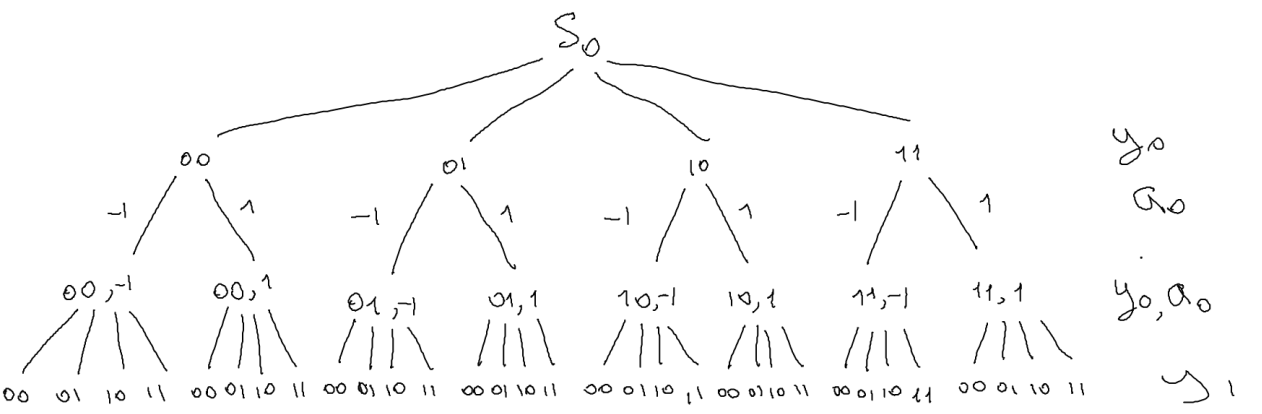
\includegraphics[width=0.5\textwidth]{../pics/ex31a.png}
\item For four nodes the state can be inferred: \\
for $[y_0 = 00, a_0 = -1, y_1 = 11]$ the only possible state is $s_1 = 0$ with $s_0 = 1$ \\
$[y_0 = 00, a_0 = 1, y_1 = 11]$ : $s_1 = 0$ $(s_0 = -1)$ \\
$[y_0 = 11, a_0 = -1, y_1 = 00]$ : $s_1 = -1$ $(s_0 = 0)$ \\
$[y_0 = 11, a_0 = 1, y_1 = 00]$ : $s_1 = 1$ $(s_0 = 0)$ \\
  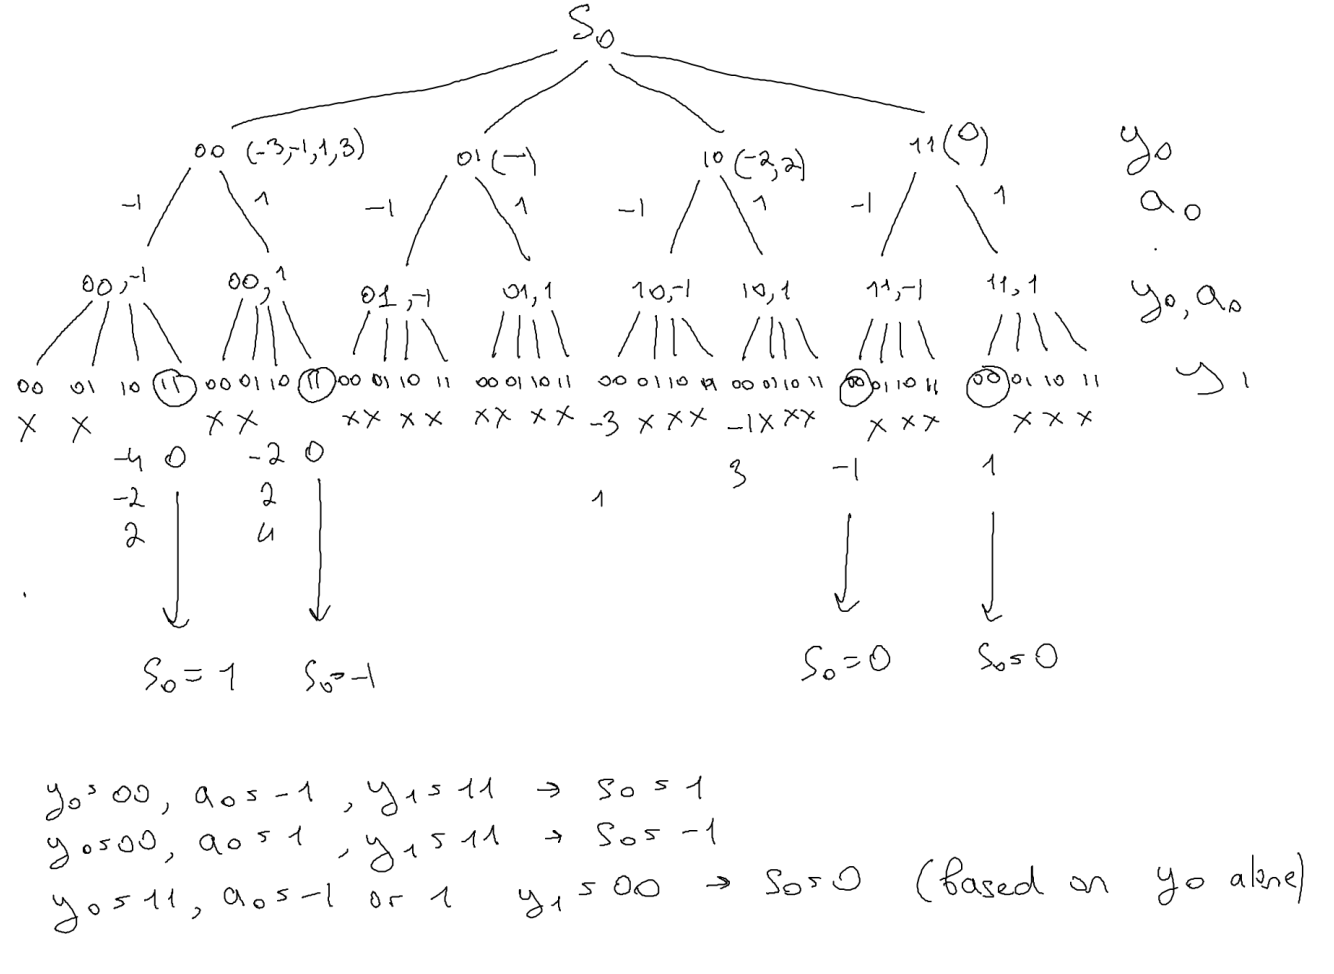
\includegraphics[width=0.5\textwidth]{../pics/ex31a2.png}
\item 24 of the 32 nodes can be pruned (marked with crosses).
\item for example the observation $y_0 = 00$ is possible for states $-3, -1, 1, 3$, the observation $y_0 = 01$ is not possible, etc (s. drawing)
\end{enumerate}


\end{solution}

%%%%%%%%%%%%%%%%%%%%%%%%%%%%%%%%%%%%%%%%%%%%%%%%%%%%%%%%%%%%%%%%%%%%%%%%%%%%%%%%

\exsection{Decision Tree for a Markov Decision Problem (3 Pts)}

Consider the following MDP:
\begin{itemize}
\item The state space is $s_t \in \ZZZ$, and the state is fullly observable.
\item The action space is $a_t \in\{-1, +1\}$
\item The state transition probabilities are
$$P(s'|s,a) = \begin{cases} .8
& \text{if~} s'=s+a \\ .2 & s'=s-a \\ 0
& \text{otherwise}\end{cases}$$
\item The initial state distribution is $P(s_0) = [s_0=0]$ (1 for $s_0=0$ and
zero otherwise)
\item The reward is binary with probability $P(r\=1|s) = [s=2]$
(reward of 1 for $s=2$ and zero otherwise)
\end{itemize}

\begin{enumerate}
\item Write (on paper) the decision tree for this domain, which has \emph{two} branchings: a 2-way branching for your decision $a_t\in\{-1,+1\}$, and a 2-way branching for the uncertain state transition.

Write down 4 levels of the tree, branching at $a_0,s_1,a_1,s_2$. (Warning: This has up to 16 leaf nodes.) You might be inclined to ``compress'' the tree into a graph -- you're welcome to do this. BUT: what if decision $a=+1$ would add a negative reward (cost) of -1. Would it then still be ok to compress the tree into a graph?)

\item What is the expected return (=sum of rewards) of first deciding $a_0=+1$ and $a_1$ uniform random, versus $a_0=-1$ and $a_1$ uniform random? (Assuming the MDP stops after two transitions.)

\item What is the best expected return one can achieve, assuming the MDP stops after two transitions.
\end{enumerate}


\begin{solution}
\begin{enumerate}
\item the tree with 4 levels:
  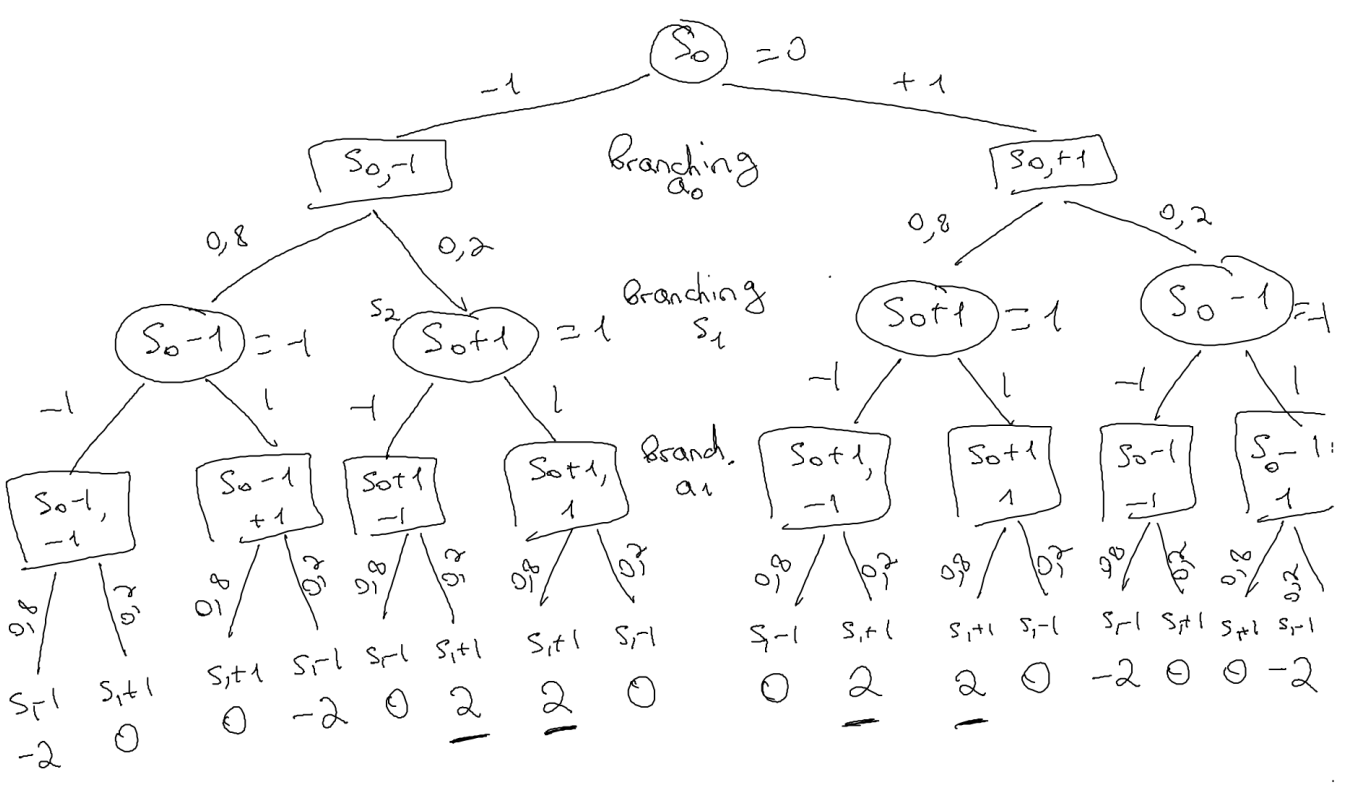
\includegraphics[width=0.5\textwidth]{../pics/ex32a.png}
\\
In the presence of a negative reward we cannot compress the tree, as every transition for decision $a=+1$ would change the accumulated reward. To calculate the reward we would need the full trajectory.

\item the expected reward for $a_0 = -1$ and $a_1$ uniform random is 0.1, with only two possible trajectories having non-zero reward \\
$E[r | a_0 = -1] = 0.2 * 0.5 * 0.2 * 1 + 0.2 * 0.5 * 0.8 * 1 + (..) * 0 = 0.1$\\
the expected reward for $a_0 = +1$ and $a_1$ uniform random is 0.4, again with only two possible trajectories having non-zero reward \\
$E[r | a_0 = +1] = 0.8 * 0.5 * 0.2 * 1 + 0.8 * 0.5 * 0.8 * 1 + (..) * 0  = 0.4$\\
\item for $a_0 = +1$ and $a_1 = +1$ the expected reward is 0.64 \\
$E[r | a_0 = +1, a_1 = +1] = 0.8 * (0.8 * 1 + 0.2 * 0) + 0.2 * 0 = 0.64$
\end{enumerate}


\end{solution}

%%%%%%%%%%%%%%%%%%%%%%%%%%%%%%%%%%%%%%%%%%%%%%%%%%%%%%%%%%%%%%%%%%%%%%%%%%%%%%%%

\exsection{Linear Regression and Bootstrapping by Hand (4 Pts)}

To be able to compute something by hand, we keep this very minimalistic here: Consider the data set $D=\{(-1,-1), (+1,+1)\}$ with just two data points $(x,y)$ with 1D input/output. Linear regression (with features $\phi(x) = (1,x)^\T$) would of course predict a linear function with slope 1 and offset 0, i.e., $f(x) = w_1 + x w_2$ with $w=(0,1)$.

\begin{enumerate}
\item Derive this solution from minimizing the loss $\sum_{i=1}^n (y_i - f(x_i))^2$ -- ideally using matrix notations to train you in this.
\item If you generate a randomized variant $\tilde D$ of the data using bootstrapping (resampling with replacement), what are the possible data sets $\tilde D$ that could be generated, and what are their probabilities?
\item What would be the optimal linear regressor for each possible $\tilde D$?
\item Now, how would you estimate confidence bounds for the prediction at $x=0$ and $x=10$, based on bootstrapping?
\end{enumerate}

\begin{solution}
    \begin{enumerate}
        \item We define $Y = \[y_1, ..., y_n\]^T$, $\Phi = \left(\begin{array}{ccc}\phi_1(x_1) & .. & \phi_F(x_1) \\ & \vdots & \\ \phi_1(x_n) & .. & \phi_F(x_n)\end{array}\right)$, $W = (w_1, ..., w_F)^T$.
        In our case, as we have two features, we have $F = 2$, and $\phi_1(x) = 1, \phi_2(x) = x$.

    In matrix notation, we can write the loss function as $||Y - \Phi W||_2$.
    To find the optimum, we compute the derivative wrt. $W$, and set it to $0$. We use $W^*$ to denote the optimal linear regressor.
    Thus, 
    $
        2\Phi^T\Phi W^* - 2\Phi^TY = 0
    $
    and finally, $W^* = (\Phi^T\Phi)^{-1}\Phi^TY$
    \item The possible datasets are $\tilde D_1 = \{(-1, -1), (-1, -1)\}$, $\tilde D_2 = \{(1, 1), (1, 1)\}$, $\tilde D_3 = \{(-1, -1), (1, 1)\}$ with probabilities $\frac{1}{4}$, $\frac{1}{4}$, $\frac{1}{2}$, respectively.
    \item We can compute the optimal linear regressor by plugging in the values of the dataset into our formula from (a).
    For $\tilde D_3$, we obtain $w = (0, 1)$.

    When plugging in the values from datasets $\tilde D_1$ or $\tilde D_2$, the matrix $(\Phi^T\Phi)$ is not invertible, and the optimum linear regressor is not uniquely defined.

    Intuitively, this makes sense, as we only a have a single unique datapoint in these two datasets.

		    \textbf{Note}: The matrix $\P^\T \P$ is not guranteed to be invertible. This happens when the columns of $\P$ are not linearly independent, so that $\P$ is not of full rank (check section 3.2 of Hastie et al., The Elements of Statistical Learning \url{https://hastie.su.domains/ElemStatLearn/}). Then $\P^\T \P$ is singular and the coefficient $W$ is not defined. A work around is to use $(\P^\T \P + \l I)$ instead of $\P^\T \P$ (section 3.4 of Hastie et al.).
    \item With bootstrapping, we would evaluate the $x$ at each point to obtain the corresponding $y$ values. From all the predictions, we can then compute the mean, and standard deviation at these points.
    \end{enumerate}

\end{solution}


%%%%%%%%%%%%%%%%%%%%%%%%%%%%%%%%%%%%%%%%%%%%%%%%%%%%%%%%%%%%%%%%%%%%%%%%%%%%%%%%

\exerfoot


\providecommand{\slides}{
  \newcommand{\slideshead}{
  \newcommand{\thepage}{\arabic{mypage}}
  %beamer
%  \documentclass[t,hyperref={bookmarks=true}]{beamer}
%  \geometry{papersize={171mm,96mm}}
  \documentclass[t,hyperref={bookmarks=true},aspectratio=169]{beamer}
  \setbeamersize{text margin left=5mm}
  \setbeamersize{text margin right=5mm}
  \usetheme{default}
  \usefonttheme[onlymath]{serif}
  \setbeamertemplate{navigation symbols}{}
  \setbeamertemplate{itemize items}{{\color{black}$\bullet$}}

  \newwrite\keyfile

  %\usepackage{palatino}
  \stdpackages
  %\usepackage{tikz} \usetikzlibrary {shapes.geometric} 
  \usepackage{multimedia}
  \usepackage[utf8]{inputenc}

  \hypersetup{
    colorlinks,
    linkcolor={blue!80!black},
    citecolor={blue!80!black},
    urlcolor={blue!80!black}
  }

  %%% geometry/spacing issues
  %\renewcommand{\baselinestretch}{1.1}
  \renewcommand{\arraystretch}{1.2}
  \columnsep 0mm

  \columnseprule 0pt
  \parindent 0ex
  \parskip 0ex
  %\setlength{\itemparsep}{3ex}
  %\renewcommand{\labelitemi}{\rule[3pt]{10pt}{10pt}~}
  %\renewcommand{\labelenumi}{\textbf{(\arabic{enumi})}}
  \setbeamertemplate{enumerate item}{(\roman{enumi})}
  \newcommand{\headerfont}{\helvetica{14}{1.5}{b}{n}}
  \newcommand{\slidefont} {\helvetica{11}{1.4}{m}{n}}
  %\newcommand{\codefont} {\helvetica{8}{1.2}{m}{n}}
  \newcommand{\urlfont} {\fontsize{6}{1.1}\selectfont}
  \renewcommand{\small} {\helvetica{10}{1.4}{m}{n}}
  \renewcommand{\tiny} {\helvetica{8}{1.3}{m}{n}}
  \newcommand{\ttiny} {\helvetica{7}{1.3}{m}{n}}

  %%% count pages properly and put the page number in bottom right
  %
  \newcounter{mypage}
  \newcommand{\incpage}{\addtocounter{mypage}{1}\setcounter{page}{\arabic{mypage}}}
  \setcounter{mypage}{0}
  \resetcounteronoverlays{page}

  \pagestyle{fancy}
  %\setlength{\headsep}{10mm}
  %\addtolength{\footheight}{15mm}
  \renewcommand{\headrulewidth}{0pt} %1pt}
  \renewcommand{\footrulewidth}{0pt} %.5pt}
  \cfoot{}
  \rhead{}
  \lhead{}
  %% \lfoot{\vspace*{-3mm}\hspace*{-3mm}\helvetica{5}{1.3}{m}{n}{\texttt{github.com/MarcToussaint/AI-lectures}}}
\lfoot{}
%  \rfoot{{\tiny\textsf{AI -- \topic -- \subtopic -- \arabic{mypage}/\pageref{lastpage}}}}
  %\lfoot{\raisebox{5mm}{\tiny\textsf{\slideauthor}}}
  %\rfoot{\raisebox{5mm}{\tiny\textsf{\slidevenue{} -- \arabic{mypage}/\pageref{lastpage}}}}
  %\rfoot{~\anchor{30,12}{\tiny\textsf{\thepage/\pageref{lastpage}}}}
  %\lfoot{\small\textsf{Marc Toussaint}}
  \rfoot{\vspace*{-4.5mm}{\tiny\textsf{\color{gray}\topic\ -- \subtopic\ -- \arabic{mypage}/\pageref{lastpage}}}\hspace*{-4mm}}
%  \rfoot{\vspace*{-4.5mm}{\tiny\textsf{\color{gray}\topic\ -- \arabic{mypage}/\pageref{lastpage}}}\hspace*{-4mm}}
%  \rfoot{~\anchor{-10,12}{\tiny\textsf{\color{gray}\topic\ --  \arabic{mypage}/\pageref{lastpage}}}}
  \lfoot{\vspace*{-4.5mm}{\hspace*{-4mm}\includegraphics[height=4mm]{LIS-26-text-long}}}

  \definecolor{grey}{rgb}{.8,.8,.8}
  \definecolor{head}{rgb}{.85,.9,.9}
%  \definecolor{blue}{rgb}{.0,.0,.5}
%  \definecolor{green}{rgb}{.0,.5,.0}
  \definecolor{red}{rgb}{.8,.0,.0}
  \definecolor{citcol}{gray}{.6}
  \newcommand{\inverted}{
    \definecolor{main}{rgb}{1,1,1}
    \color{main}
    \pagecolor[rgb]{.3,.3,.3}
  }
  \input{../latex/macros}

  \graphicspath{{pics/}{../pics/}{pics-local/}}
}

\newcommand{\slidestitle}{
  \title{\course \topic}
  \author{Marc Toussaint}
  \institute{Learning \& Intelligent Systems Lab, TU Berlin}

  \begin{document}


  %% title slide!
  \slide{}{
    \thispagestyle{empty}

    \twocol{.35}{.55}{
      %\vspace*{-5mm}%
      \hspace*{-5mm}%
      \includegraphics[width=1.\columnwidth]{\coursepicture}
    }{\center

      \textbf{\fontsize{17}{20}\selectfont \course}

      ~

      %Lecture
      \topic\\

      \vspace{1cm}

      {\tiny~\emph{\keywords}~\\}

      \vspace{1cm}

      \teacher
      
      Technical University of Berlin

      \coursedate

      ~

    }
  }
}

\newcommand{\slide}[2]{
  \slidefont
  \incpage\begin{frame}
  \addcontentsline{toc}{section}{#1}
  \vfill
  {\headerfont #1} \vspace*{-2ex}
  \begin{itemize}\item[]~\\
    #2
  \end{itemize}
  \vfill
  \end{frame}
}

% use \begin{frame}[fragile] around slidecore!
\newenvironment{slidecore}[1]{
  \slidefont\incpage
  \addcontentsline{toc}{section}{#1}
  \vfill
  {\headerfont #1} \vspace*{-2ex}
  \begin{itemize}\item[]~\\
}{
  \end{itemize}
  \vfill
}

\newcommand{\titleslide}[4][Marc Toussaint]{
  \newcommand{\slideauthor}{#1}
  \newcommand{\slidevenue}{#3}
  \slidefont
  \incpage
  \begin{frame}
  \begin{center}
    \vspace*{15mm}

    {\headerfont #2\\}
        
    \vspace*{10mm}

    #1 \\

    \vspace*{5mm}

    {\small
      Learning \& Intelligent Systems Lab, TU Berlin\\
%      Science of Intelligence Cluster of Excellence, Berlin\\
      Max Planck Fellow, Institute for Intelligent Systems\\ %Physical Reasoning \& Manipulation Lab -- 
%      MIT CSAIL\\
%      mtoussai@mit.edu,~ marc.toussaint@informatik.uni-stuttgart.de

      \vspace*{10mm}

      \emph{#3}
    }

    \vspace*{0mm}

    %\includegraphics[scale=.1]{pics/eushield-fullcolour}

  \end{center}
  \begin{itemize}\item[]~\\
    #4
  \end{itemize}
  \end{frame}
}

\newcommand{\titleslideempty}[2]{
  \slidefont
  \incpage
  \begin{frame}
  \begin{center}
    \vspace*{15mm}

    {\headerfont #1\\}
        
    %% \vspace*{5mm}

    %% {\small\emph{#2}} \\

  \end{center}
  \begin{itemize}\item[]~\\
    #2
  \end{itemize}
  \end{frame}
}

\providecommand{\key}[1]{
  \addtocounter{mypage}{1}
% \immediate\write\keyfile{#1}
  \addtocontents{toc}{\hyperref[key:#1]{#1 (\arabic{mypage})}}
%  \phantomsection\label{key:#1}
%  \index{#1@{\hyperref[key:#1]{#1 (\arabic{mysec}:\arabic{mypage})}}|phantom}
  \addtocounter{mypage}{-1}
}

\providecommand{\course}{}

\providecommand{\subtopic}{}

\providecommand{\sublecture}[2]{
  \renewcommand{\subtopic}{#1}
  \slide{#1}{#2}
}

\providecommand{\sublectureHide}[2]{
  \renewcommand{\subtopic}{#1}
}

\providecommand{\story}[1]{
~

Motivation: {\tiny #1}\clearpage
}

\newenvironment{items}[1][9]{
\par\setlength{\unitlength}{1pt}\fontsize{#1}{#1}\linespread{1.2}\selectfont
\begin{list}{--}{\leftmargin4ex \rightmargin0ex \labelsep1ex \labelwidth2ex
\topsep.7ex \parsep0ex \itemsep3pt}
}{
\end{list}
}

\newenvironment{itemS}[1][4ex]{
\par
\tiny
\begin{list}{--}{\leftmargin#1 \rightmargin0ex \labelsep1ex
  \labelwidth2ex \topsep0pt \parsep0ex \itemsep2pt}
}{
\end{list}
}

\providecommand{\slidesfoot}{
  \end{document}
}


  \slideshead
  \lecturetitleslide
}

\providecommand{\exercises}{
  \newcommand{\exerciseshead}{
  \documentclass[10pt,fleqn]{article}
  \stdpackages
\usepackage[utf8]{inputenc}

  \definecolor{bluecol}{rgb}{0,0,.5}
  \definecolor{greencol}{rgb}{0,.4,0}
  \definecolor{shadecolor}{gray}{0.9}
  \usepackage[
    %    pdftex%,
    %%    letterpaper,
    %    bookmarks,
    %    bookmarksnumbered,
    colorlinks,
    urlcolor=bluecol,
    citecolor=black,
    linkcolor=bluecol,
    %    pagecolor=bluecol,
    pdfborder={0 0 0},
    %pdfborderstyle={/S/U/W 1},
    %%    backref,     %link from bibliography back to sections
    %%    pagebackref, %link from bibliography back to pages
    %%    pdfstartview=FitH, %fitwidth instead of fit window
    pdfpagemode=UseNone, %UseOutlines, %bookmarks are displayed by acrobat
    pdftitle={\course},
    pdfauthor={Marc Toussaint},
    pdfkeywords={}
  ]{hyperref}
  \DeclareGraphicsExtensions{.pdf,.png,.jpg,.eps}

  \renewcommand{\r}{\varrho}
  \renewcommand{\l}{\lambda}
  \renewcommand{\L}{\Lambda}
  \renewcommand{\b}{\beta}
  \renewcommand{\d}{\delta}
  \renewcommand{\k}{\kappa}
  \renewcommand{\t}{\theta}
  \renewcommand{\O}{\Omega}
  \renewcommand{\o}{\omega}
  \renewcommand{\SS}{{\cal S}}
  \renewcommand{\=}{\!=\!}
  %\renewcommand{\boldsymbol}{}
  %\renewcommand{\Chapter}{\chapter}
  %\renewcommand{\Subsection}{\subsection}

  \renewcommand{\baselinestretch}{1.1}
  \geometry{a4paper,headsep=7mm,hdivide={15mm,*,15mm},vdivide={20mm,*,15mm}}

  \fancyhead[L]{\thetitle, \textit{\teacher}---\coursedate}
  \fancyhead[R]{\thepage}
  \fancyhead[C]{}
  \fancyfoot{}
  \pagestyle{fancy}

  \renewcommand{\labelenumi}{{\alph{enumi})}}

  \parindent 0pt
  \parskip 0.5ex

  \newcommand{\codefont}{\helvetica{8}{1.2}{m}{n}}
  \newcommand{\urlfont} {\fontsize{6}{1.1}\selectfont}
  \newcommand{\ttiny} {\helvetica{7}{1.3}{m}{n}}

  \input{../latex/macros}

  \DefineShortVerb{\@}

  \usepackage{comment}
  \specialcomment{solution}{
    \small
    \begin{shaded}
  }{
    \end{shaded}
  }
  
  \renewcommand{\hat}{\widehat}
  \newcommand{\bbg}{{\bar{\bar g}}}
  \graphicspath{{pics/}{../pics/}}

  \mytitle{\course\\\exnum}
  \myauthor{\teacher\\ \small\addressTUB}
  \date{\coursedate}
}

%%%%%%%%%%%%%%%%%%%%%%%%%%%%%%%%%%%%%%%%%%%%%%%%%%%%%%%%%%%%%%%%%%%%%%%%%%%%%%%%

\newcommand{\exercisestitle}{  
  \begin{document}
  \maketitle
}

\newcommand{\exsection}[1]{\section{#1}}

\newcommand{\exsubsection}[1]{\subsection{#1}}

\newcommand{\exerfoot}{
  \end{document}
}

\newenvironment{items}[1][9]{
  \par\setlength{\unitlength}{1pt}\fontsize{#1}{#1}\linespread{1.2}\selectfont
  \begin{list}{--}{\leftmargin4ex \rightmargin0ex \labelsep1ex \labelwidth2ex
      \topsep0pt \parsep0ex \itemsep3pt}
}{
  \end{list}
}

  \exerciseshead
}

\providecommand{\script}{
  \newcommand{\scripthead}{
  \documentclass[9pt,fleqn,twoside]{article}
  \stdpackages

  \usepackage{makeidx}
  \makeindex

  \usepackage{thmtools}
  \definecolor{shadecolor}{gray}{0.85}
  \declaretheoremstyle[
    %headfont=\normalfont\bfseries,
    %notefont=\mdseries, notebraces={(}{)},
    %bodyfont=\normalfont,
    %postheadspace=0.5em,
    %spaceabove=6pt,
    mdframed={
      %  skipabove=8pt,
      %  skipbelow=6pt,
      hidealllines=true,
      backgroundcolor={shadecolor},
      innertopmargin=8pt,
      %  innerleftmargin=3pt,
      %  innerrightmargin=3pt
    }
  ]{shaded}
  \declaretheorem[style=shaded,within=section,name=Definition]{myDefinition}
  \declaretheorem[style=shaded,within=section,name=Theorem]{myTheorem}
  \declaretheorem[style=shaded,within=section,name=Identities]{Identities}
  \declaretheorem[style=shaded,within=section,name=Example]{myExample}

  \definecolor{grey}{rgb}{.8,.8,.8}
  \definecolor{bluecol}{rgb}{0,0,.5}
  \definecolor{greencol}{rgb}{0,.4,0}
  \definecolor{shadecolor}{gray}{0.9}
  \definecolor{citcol}{rgb}{.4,.4,.4}
  \usepackage[
    %    pdftex%,
    %%    letterpaper,
    %bookmarks,
    bookmarksnumbered,
    colorlinks,
    urlcolor=bluecol,
    citecolor=black,
    linkcolor=bluecol,
    %    pagecolor=bluecol,
    pdfborder={0 0 0},
    %pdfborderstyle={/S/U/W 1},
    %%    backref,     %link from bibliography back to sections
    %%    pagebackref, %link from bibliography back to pages
    %%    pdfstartview=FitH, %fitwidth instead of fit window
    pdfpagemode=UseOutlines, %bookmarks are displayed by acrobat
    pdftitle={\course},
    pdfauthor={Marc Toussaint},
    pdfkeywords={}
  ]{hyperref}
  \DeclareGraphicsExtensions{.pdf,.png,.jpg,.eps}

  %\usepackage{multirow}
  \usepackage{multimedia}
  %\usepackage{marginnote}
  %\setbeamercolor{background canvas}{bg=}

  \usepackage[round]{natbib}
  \bibliographystyle{abbrvnat}

  \renewcommand{\r}{\varrho}
  \renewcommand{\l}{\lambda}
  \renewcommand{\L}{\Lambda}
  \renewcommand{\b}{\beta}
  \renewcommand{\d}{\delta}
  \renewcommand{\k}{\kappa}
  \renewcommand{\t}{\theta}
  \renewcommand{\O}{\Omega}
  \renewcommand{\o}{\omega}
  \renewcommand{\SS}{{\cal S}}
  \renewcommand{\=}{\!=\!}
  %\renewcommand{\boldsymbol}{}
  %\renewcommand{\Chapter}{\chapter}
  %\renewcommand{\Subsection}{\subsection}

  \renewcommand{\baselinestretch}{1.0}
  \geometry{a5paper,headsep=6mm,hdivide={10mm,*,10mm},vdivide={13mm,*,7mm}}

  \fancyhead[OL,ER]{\course, \textit{Marc Toussaint}}
  \fancyhead[OR,EL]{\thepage}
  \fancyhead[C]{}
  \fancyfoot{}
  \pagestyle{fancy}

  \renewcommand{\labelenumi}{{(\roman{enumi})}}
  \renewcommand{\theenumi}{(\roman{enumi})} %for ref
  \parindent 0pt
  \parskip .5pc

  \columnsep 6ex

  \renewcommand{\familydefault}{\sfdefault}

  \newcommand{\headerfont}{\large}%helvetica{12}{1}{b}{n}}
  \newcommand{\slidefont} {}%\helvetica{9}{1.3}{m}{n}}
  \newcommand{\storyfont} {}
  %  \renewcommand{\small}   {\helvetica{8}{1.2}{m}{n}}
  \renewcommand{\tiny}    {\footnotesize}%helvetica{7}{1.1}{m}{n}}
  \newcommand{\ttiny} {\footnotesize}%fontsize{7}{7}\selectfont}
%  \newcommand{\codefont}{\fontsize{6}{6}\selectfont}%helvetica{8}{1.2}{m}{n}}
  \newcommand{\codefont} {\helvetica{8}{1.2}{m}{n}}

  \input{../latex/macros}

  \usepackage{comment}
  \specialcomment{solution}{
    \small
    \begin{shaded}
  }{
    \end{shaded}
  }

  \graphicspath{{pics/}{../latex/pics/}}

  \mytitle{\course\\Lecture Script}
  \myauthor{Marc Toussaint}
  \date{\coursedate}
}

%%%%%%%%%%%%%%%%%%%%%%%%%%%%%%%%%%%%%%%%%%%%%%%%%%%%%%%%%%%%%%%%%%%%%%%%%%%%%%%%

\newcommand{\scripttitle}{
  \begin{document}
  \maketitle
  %\anchor{100,10}{\includegraphics[width=4cm]{optim}}
%  \vspace*{1cm}

  \emph{This is a direct concatenation and reformatting of all lecture
    slides and exercises from this course, including indexing to help
    prepare for exams.}

  {\tableofcontents}
}

%%%%%%%%%%%%%%%%%%%%%%%%%%%%%%%%%%%%%%%%%%%%%%%%%%%%%%%%%%%%%%%%%%%%%%%%%%%%%%%%

\newcounter{mypage}
\setcounter{mypage}{0}
\newcommand{\incpage}{\addtocounter{mypage}{1}}

\newcommand{\subtopic}{}
\newcommand{\pause}{}
\newcommand{\only}[1]{#1}

\renewcommand{\slides}[1][]{
  %  \clearpage
  \subsection{\topic}
  \index{\topic}
  {\small #1}
  \setcounter{mypage}{0}
  \smallskip\nopagebreak\hrule\medskip
}

\newcommand{\slidesfoot}{
  \bigskip
}

\newcommand{\sublecture}[2]{
  \index{#1}
}

\newcommand{\key}[1]{
  \phantomsection\addcontentsline{toc}{subsubsection}{#1}
  %\subsubsection{#1}
  \index{#1}
}

\providecommand{\defn}[1]{%
  \textbf{#1}\index{#1}%
}

\newenvironment{slidecore}[1]{
  \incpage
  \subsubsection*{#1}%{\headerfont\noindent\textbf{#1}\\}%
  \vspace{-6ex}%
  \begin{list}{$\bullet$}{\leftmargin4ex \rightmargin0ex \labelsep1ex
    \labelwidth2ex \partopsep0ex \topsep0ex \parsep.5ex \parskip0ex \itemsep0pt}\item[]~\\\nopagebreak%
}{
  \end{list}\nopagebreak%
  {\hfill\tiny \textsf{\arabic{section}.\arabic{subsection}:\arabic{mypage}}}\nopagebreak%
  \smallskip\nopagebreak\hrule
}

\newcommand{\slide}[2]{
  \begin{slidecore}{#1}
    #2
  \end{slidecore}
}

\renewcommand{\exercises}{}
\newcommand{\exercisestitle}{}
\newcommand{\exsection}[1]{\subsubsection{#1}}
\newcommand{\exerfoot}{\bigskip}

\newcommand{\story}[1]{
  \subsection*{Motivation \& Outline}
  {\storyfont\sf #1}
  \medskip\nopagebreak\hrule
}

\newcounter{savedsection}
\newcommand{\subappendix}{\setcounter{savedsection}{\arabic{section}}\appendix}
\newcommand{\noappendix}{
  \setcounter{section}{\arabic{savedsection}}% restore section number
  \setcounter{subsection}{0}% reset section counter
%  \gdef\@chapapp{\sectionname}% reset section name
  \renewcommand{\thesection}{\arabic{section}}% make section numbers arabic
}

\newenvironment{items}[1][9]{
\par\setlength{\unitlength}{1pt}\fontsize{#1}{#1}\linespread{1.2}\selectfont
\begin{list}{--}{\leftmargin4ex \rightmargin0ex \labelsep1ex \labelwidth2ex
\topsep0pt \parsep0ex \itemsep3pt}
}{
\end{list}
}

\newcommand{\Def}[1]{%
\textbf{#1}\index{#1}}%\marginnote{#1}}

  \scripthead
}

\providecommand{\note}{
  \providecommand{\notehead}[2]{
  \documentclass[#1,fleqn,twoside]{article}
  \stdpackages
  \renewcommand{\labelenumi}{{(\roman{enumi})}}
  \renewcommand{\theenumi}{(\roman{enumi})} %for ref

  \renewcommand{\baselinestretch}{#2}
  \renewcommand{\arraystretch}{1.2}
  \renewcommand{\topfraction}{1}
  \renewcommand{\bottomfraction}{1}
  \renewcommand{\textfraction}{0}
  \columnsep 5ex
  \parindent 3ex
  \parskip 1ex

  % Lists and paragraphs
  \parindent 0pt
  \topsep 4pt plus 1pt minus 2pt
  \partopsep 1pt plus 0.5pt minus 0.5pt
  \itemsep 2pt plus 1pt minus 0.5pt
  \parsep 2pt plus 1pt minus 0.5pt
  \parskip .5pc %add _in_ {thebibliography} environment in *.bbl

  \setcounter{tocdepth}{3}
  \setcounter{secnumdepth}{3}

  \geometry{a4paper,hdivide={25mm,*,25mm},vdivide={25mm,*,25mm}}

  \renewcommand{\headrulewidth}{.0pt}\renewcommand{\footrulewidth}{.0pt}\cfoot{}
  \fancyhead[OL,EC]{\it\theauthor---\today}
  \fancyhead[ER]{\leftmark}
  \fancyhead[OR,EL]{\thepage}
  \fancyfoot[EL,OR]{}
  \setlength{\headsep}{10mm}
  %\fancyhead[OL]{\rightmark}
  %\fancyfoot[EL,OR]{}


  %  \usepackage{palatino}

  \newcommand{\codefont}{\helvetica{8}{1.2}{m}{n}}

  \renewenvironment{abstract}{
    \vspace*{5ex}\begin{list}{}{
      \leftmargin3ex
      \rightmargin3ex
      \topsep-\parskip}\item[]
     \hrule\vspace{1.5ex}{\bf Abstract.~}\small}
    {\vspace{2ex}\hrule\end{list}\vspace{5ex}}
    
  \newenvironment{keyword}
    {\par{\it Keywords:~}}
    {}

  \def\makemytitle{%
    \thispagestyle{empty}
    \begin{list}{}{\leftmargin3ex \rightmargin3ex \topsep0ex \parsep0ex}\item[]
      \begin{center}
        {\fontsize{18}{25}\selectfont{\thetitle\\}}\vspace{5ex}

        {\fontsize{14}{16}\selectfont{\theauthor\\}}\vspace{1ex}

        {\footnotesize{\sl \addressFUB}\\ \emailBerlin}

        {\footnotesize \today}

        \vspace{1ex}
        {\small \published}
      \end{center}
    \end{list}
    \renewcommand{\maketitle}{\chapter{\thetitle}}
  }

  \input{../latex/macros}
  \pdflatex

  \graphicspath{{pics/}{../pics/}{pics-local/}}

  \myauthor{Marc Toussaint}
  \date{\today}
}

%%%%%%%%%%%%%%%%%%%%%%%%%%%%%%%%%%%%%%%%%%%%%%%%%%%%%%%%%%%%%%%%%%%%%%%%%%%%%%%%

\newcommand{\notetitle}{
  \begin{document}
  \thispagestyle{empty}
    
  \maketitle

}

\newenvironment{items}[1][9]{
\par\setlength{\unitlength}{1pt}\fontsize{#1}{#1}\linespread{1.2}\selectfont
\begin{list}{--}{\leftmargin4ex \rightmargin0ex \labelsep1ex \labelwidth2ex
\topsep0pt \parsep0ex \itemsep3pt}
}{
\end{list}
}

  \notehead{10}{1.1}
}

\providecommand{\course}{NO COURSE}
\providecommand{\coursepicture}{NO PICTURE}
\providecommand{\coursedate}{NO DATE}
\providecommand{\topic}{NO TOPIC}
\providecommand{\keywords}{NO KEYWORDS}
\providecommand{\exnum}{NO NUMBER}
\providecommand{\teacher}{Marc Toussaint}

\providecommand{\stdpackages}{
  \usepackage{amsmath}
  \usepackage{amssymb}
  \usepackage{amsfonts}
  \allowdisplaybreaks
  \usepackage{amsthm}
  \usepackage{eucal}
  \usepackage{graphicx}
  \usepackage{color}
  \usepackage{geometry}
  \usepackage{framed}
%  \usecolor{xcolor}
  \definecolor{shadecolor}{gray}{0.9}
  \setlength{\FrameSep}{3pt}
  \usepackage{fancyvrb}
  \fvset{numbers=none,xleftmargin=5ex}

  \usepackage{pdfpages}

  \usepackage{multicol} 
  \usepackage{fancyhdr}
}

\providecommand{\addressUSTT}{
  Machine~Learning~\&~Robotics~lab, U~Stuttgart\\\small
  Universit{\"a}tsstra{\ss}e 38, 70569~Stuttgart, Germany
}

\providecommand{\addressTUB}{
  Learning~\&~Intelligent~Systems~Lab, TU~Berlin\\\small
  Marchstr. 23, 10587 Berlin, Germany
}


\renewcommand{\course}{Artificial Intelligence}
\renewcommand{\coursepicture}{course_ai}
\renewcommand{\coursedate}{Summer 2026}

\renewcommand{\exnum}{Exercise 5}

\exercises
\excludecomment{solution}
\exercisestitle

%%%%%%%%%%%%%%%%%%%%%%%%%%%%%%%%%%%%%%%%%%%%%%%%%%%%%%%%%%%%%%%%%%%%%%%%%%%%%%%%

\exsection{Happy ever after}

Consider a mini mini MDP with just three states $s\in\{0,1,2\}$, where there agent receives reward $R(0,a)=R(1,a)=0$ in state $0$ and $1$, and reward $R(2,a)=1$ in state $2$ (independent of $a$). For simplicity we assume everything is deterministic and the policy $\pi$ deterministically walks from state $0$ to $1$ to $2$ and then stays in state $2$ happily forever. (No need to define actions explicitly; the resulting state sequence when initialized in $s_0=0$ is always $(s_0=0, s_1=1, s_2=2, s_3=2, ...)$.
We have some discount factor $\g\in[0,1)$.

\begin{enumerate}
	\item What are the values $V^\pi(s=2)$ and $V^\pi(s=1)$ and $V^\pi(s=0)$? Derive this analytically by the definition $V^\pi(s) = \Exp{ \tsum_t \g^t r_t \| s_0\=s; \pi }$ and knowing about convergence of the geometric series.
\end{enumerate}

\begin{solution}
    We use the given definition, and the knowledge that the process and the policy is deterministic. Thus
    $V^\pi(s) = \Exp{ \tsum_t \g^t r_t \| s_0 = s ; \pi } = \tsum_t \g^t r_t$, and we can plug in the values:

    \begin{itemize}
        \item $V^\pi(s=2) = \tsum_t \g^t \cdot 1 = 1 + \g + \g^2 + ... = \frac{1}{1 - \g}$.
        \item $V^\pi(s=1) = \tsum_t \g^t \cdot 1 = 0 + \g + \g^2 + ... = \g(1 + \g + \g^2 + ...) = \frac{\g}{1 - \g}$.
        \item $V^\pi(s=0) = \tsum_t \g^t \cdot 1 = 0 + 0 + \g^2 + ... = \g^2(1 + \g + \g^2 + ...) = \frac{\g^2}{1 - \g}$.
    \end{itemize}
\end{solution}


%%%%%%%%%%%%%%%%%%%%%%%%%%%%%%%%%%%%%%%%%%%%%%%%%%%%%%%%%%%%%%%%%%%%%%%%%%%%%%%%

\exsection{Value Iteration}

\show[.3]{../pics/Maze.pdf}

Consider the circle of states above, which depicts the 8 states $s\in\{1,..,8\}$ of an
MDP. The following describes the MDP informally. Your first exercise will let you write down explicitly the probability \& reward tables $P(s_0), P(s'|s,a), R(s,a)$. Consider a discounting of $\g=1/2$.

Description of $P(s'|s,a)$:\NewParNoBreak
\begin{itemize}
\item The agent can choose between two actions $a\in\{-1,+1\}$: going one step clock-wise ($a=+1$) or one step counter-clock-wise ($a=-1$).
\item With probability $3/4$ the agent will transition to the desired state,
  with probability $1/4$ to the state in the opposite direction.
\item Exception: When $s=1$ (the green state) the next state will always be
$s'=4$, independent of $a$. The Markov Decision Process never ends.
\end{itemize}

Description of $R(s,a)$:\NewParNoBreak
\begin{itemize}
\item The agent receives a reward of $r=4096$ when $s=1$ (the green state).
\item The agent receives a reward of $r=-512$ when $s=2$ (the red state).
\item The agent receives zero reward otherwise.
\end{itemize}

Description of $P(s_0)$:\NewParNoBreak
\begin{itemize}
\item The agent deterministically starts in $s_0=4$
\end{itemize}

Exercise:
\begin{enumerate}
\item Explicitly provide the probability/reward tables $P(s_0), P(s'|s,a), R(s,a)$ that define this MDP.

\item Perform three steps of Value Iteration to approximate the optimal value function $V^*$: Initialize $V_{k=0}(s)=0$, what is
  $V_{k=1}(s)$, $V_{k=2}(s)$, $V_{k=3}(s)$?

{\small Tip: Write the value functions explicitly as tables on paper, starting with $V_0 = [0 ~ 0 ~ 0 ~ 0 ~ 0 ~ 0 ~ 0 ~ 0]$, and then $V_1$ below (which is still easy since only immediate rewards enter), and then $V_2$ below, etc.

}
  
%% \item How can you compute the value function $V^\pi(s)$ for
%% a GIVEN policy (e.g., always walk clock-wise) in closed form? Provide
%% an explicit matrix equation.

\item Assume you are given $V^*(s)$. How can you compute the optimal $Q^*(s,a)$
  form this? And assume $Q^*(s,a)$ is given, how can you compute the optimal
  $V^*(s)$ from this? Just recall the provided equations.

\item What is $Q_{k=3}(s,a)$ for the example above? (Write this on paper as an 8x2 table, or 2x8 if you like.) What is the
  ``optimal'' policy given $Q_{k=3}$?
\end{enumerate}

\begin{solution}
    \begin{enumerate}
        \item The probability table for the initial state is 

\begin{tabular}{l|l}
$s_0$ & $P(s_0)$ \\ \hline
1    & 0       \\
2    & 0       \\
3    & 0       \\
4    & 1       \\
5    & 0       \\
6    & 0       \\
7    & 0       \\
8    & 0      
\end{tabular}

The reward table is

\begin{tabular}{l|ll}
$s$ / $a$ & -1   & 1    \\ \hline
1 & 4096 & 4096 \\
2 & -512 & -512 \\
3 & 0    & 0    \\
4 & 0    & 0    \\
5 & 0    & 0    \\
6 & 0    & 0    \\
7 & 0    & 0    \\
8 & 0    & 0
\end{tabular}

and finally, the transition probability table is 

\begin{tabular}{l|llllllll}
    $(s,a)$ / $s'$ & 1   & 2 & 3 & 4 & 5 & 6 & 7 & 8    \\ \hline
    (1, -1) & 0 & 0 & 0 & 1 & 0 & 0 & 0 & 0 \\
    (1, 1) & 0 & 0 & 0 & 1 & 0 & 0 & 0 & 0 \\ \hline
    (2, -1) & $\frac{3}{4}$ & 0 & $\frac{1}{4}$ & 0 & 0 & 0 & 0 & 0 \\
    (2, 1) & $\frac{1}{4}$ & 0 & $\frac{3}{4}$ & 0 & 0 & 0 & 0 & 0 \\ \hline
    (3, -1) & 0 & $\frac{3}{4}$ & 0 & $\frac{1}{4}$ & 0 & 0 & 0 & 0 \\
    (3, 1) & 0 & $\frac{1}{4}$ & 0 & $\frac{3}{4}$ & 0 & 0 & 0 & 0  \\ \hline
    (4, -1) & 0 & 0 & $\frac{3}{4}$ & 0 & $\frac{1}{4}$ & 0 & 0 & 0 \\
    (4, 1) & 0 & 0 & $\frac{1}{4}$ & 0 & $\frac{3}{4}$ & 0 & 0 & 0  \\ \hline
    (5, -1) &0 &0 & 0 & $\frac{3}{4}$ & 0 & $\frac{1}{4}$ & 0 & 0 \\
    (5, 1) &0 & 0&0 & $\frac{1}{4}$ & 0 & $\frac{3}{4}$ & 0 & 0  \\ \hline
    (6, -1) & 0& 0& 0&0 & $\frac{3}{4}$ & 0 & $\frac{1}{4}$ & 0\\
    (6, 1) & 0& 0& 0&0 & $\frac{1}{4}$ & 0 & $\frac{3}{4}$ & 0  \\ \hline
    (7, -1) & 0&0 &0 & 0&0 & $\frac{3}{4}$ & 0 & $\frac{1}{4}$\\
    (7, 1) & 0&0 &0 &0 &0 & $\frac{1}{4}$ & 0 & $\frac{3}{4}$  \\ \hline
    (8, -1)  & $\frac{1}{4}$& 0&0 &0 &0 &0 & $\frac{3}{4}$ & 0\\
    (8, 1)  & $\frac{3}{4}$ &0 &0 &0 &0 &0 & $\frac{1}{4}$ & 0 
\end{tabular}

        \item The values are computed with $V_{k+1}(s) = \max_a \[R(s, a) + \g\sum_{s'}P(s'|s,a)V_k(s')\]$.
            
            The resulting table is

\begin{tabular}{l|llllllll}
     & 1   & 2 & 3 & 4 & 5 & 6 & 7 & 8    \\ \hline
    $V_{k=0}(s)$ & 0 & 0 & 0 & 0 & 0 & 0 & 0 & 0 \\
    $V_{k=1}(s)$ & 4096 & -512 & 0 & 0 & 0 & 0 & 0 & 0 \\
    $V_{k=2}(s)$ & 4096 & 1024 & -64 & 0 & 0 & 0 & 0 & 1536 \\
    $V_{k=3}(s)$ & 4096 & 1016 & 384 & -8 & 0 & 0 & 576 & 1536 \\
\end{tabular}

We give two examples how the values are computed with the formula above:
\begin{align*}
    V_2(s=2) &= \max\[-512 + \g (P(1|2,1)V_1(1) + P(3|2,1)V_1(3)), -512 + \g (P(1|2,-1)V_1(1) + P(3|2,-1)V_1(3))\]\\
             &= \max\[-512 + \frac{1}{2} \frac{3}{4}\cdot 4096, -512 +\frac{1}{2} \frac{1}{4}\cdot 4096\]\\
             &= 1024
\end{align*}
%
\begin{align*}
    V_3(s=2) &= \max\[-512 + \g (P(1|2,1)V_2(1) + P(3|2,1)V_2(3)), -512 + \g (P(1|2,-1)V_2(1) + P(3|2,-1)V_2(3))\]\\
             &= \max\[-512 + \frac{1}{2} \cdot\frac{3}{4}\cdot 4096 + \frac{1}{2}\cdot\frac{1}{4}\cdot(-64),-512 + \frac{1}{2} \cdot\frac{1}{4}\cdot 4096 + \frac{1}{2}\cdot\frac{3}{4}\cdot(-64)\]\\
             &= 1016
\end{align*}

        \item The relations are $V^*(s) = \max_a Q^*(s,a)$, and $Q^*(s,a) = R(s,a) + \g \Exp[s'\sim P(\cdot|s,a)]{V^*(s')}$
        \item We can plug in the values in the relation 
            %
            \begin{equation}
                Q_{k+1}(s,a) = R(s,a) + \g \sum_{s'}P(s'|s,a)V_{k}(s')
            \end{equation}
%
            to obtain
%

\begin{tabular}{l|lll}
    $s$ / $a$ & -1   & 1 & $\max_a$   \\ \hline
    1 & 4092 & 4092 & $\{-1, 1\} $\\
    2 & 1016 & -24 & -1 \\
    3 & 384 & 128 & -1 \\
    4 & -24 & -8 & 1\\
    5 & 0 & 0 & $\{-1, 1\} $\\
    6 & 0  & 0 & $\{-1, 1\} $\\
    7 & 192 & 576  & 1\\
    8 & 728 & 1608 & 1
\end{tabular}
    \end{enumerate}
\end{solution}

%%%%%%%%%%%%%%%%%%%%%%%%%%%%%%%%%%%%%%%%%%%%%%%%%%%%%%%%%%%%%%%%%%%%%%%%%%%%%%%%

\exsection{Episodes \& terminal states}

The formal MDP theory typically assumes that we talk about an infinite process\\ $s_0,a_0,r_0,s_1,a_1,r_1,...$ of states, actions and rewards. Consistent to that, the return is formally defined as the infinite sum $\sum_{t=0}^\infty \g^t r_t$.

However, practical problems in the literature often involve ``terminal states'', and one speaks of ``episodes''. The following exercise clarifies how ``terminal states'' and ``episodes'' are meant in an infinite MDP.

\begin{enumerate}
\item Let us define that a terminal state as follows: Assume that in step $T$ the agent reaches a terminal state $s_T$. The agent can then make a very last action $a_T$, and gets a final reward with expectation $r_T = R(s_T, a_T)$, but after this ``there are no more states, actions, or rewards'', and the total return of the agent is $\sum_{t=0}^T \g^t r_t$.

At first sight this is inconsistent to how MDPs are defined, because by definition they do not terminate. How can you construct a formal MDP to model such terminal states? (Tip: Extend the state space.)

\begin{solution}
We can add a `Nirvana' state to the MDP; informally, the nirvana state $s_N$ has the properties
    \begin{itemize}
        \item the terminal state transitions to the nirvana state for any action.
        \item one cannot escape from the nirvana state
        \item there is no reward in the nirvana state
    \end{itemize}

    The reward then becomes $\sum_{t=0}^\infty \g^t r_t = \sum_{t=0}^T \g^t r_t + \sum_{t=T+1}^\infty \g^t \cdot 0 = \sum_{t=0}^T \g^t r_t$
\end{solution}

%\item In practise one never runs (or simulates) a process infinitely long. Instead, one typically aborts at some finite horizon $T$ (or when a terminal state is reached). One such aborted run is called \emph{episode}. One then typically repeats many episodes (to collect data for learning or estimation of values/performance).
%
%Consider an MDP where the goal state is a \emph{tunnel state}, which means that every choice of action in the goal state leads to a state transition back to a (maybe random) initial state $s\sim P(s_0)$.
%
%Is the optimal policy for the MDP with tunnel goal state the same as the optimal policy for an MDP where the goal state is a terminal state? Provide arguments (ideally a rough proof or counterexample) for your answer.
%
%\begin{solution}
%We want to answer the question if the optimal policy in the case above is the same as if we'd continue to run the MDP infintely long, i.e, we want to know if
%
%    $$\pi^*_{\infty} = \argmax_\pi \Exp{\sum_{t=0}^T\g^tr_t| s_0\sim P_0, s_{t+1}\sim P(\cdot | s_t, a_t), a_t\sim \pi(s_t)}$$
%
%    (where we assumed that the reward at the terminal state will be 0 for the rest of the episode, after the state is reached at time $T$) is equal to the policy that we obtain if we `tunnel' back to the (random) starting state.
%    We can compute the tunnel-policy as
%
%    %$$\pi^*_{tunnel} = \argmax_\pi \sum_{i=0}^\infty \Exp{\sum_{t=0}^{T_0} \g^tr_t| s_0\sim P_0, s_{t+1}\sim P(\cdot | s_t, a_t)}$$
%
%    $$\pi^*_{tunnel} = \argmax_\pi \sum_{i=0}^\infty \Exp{\sum_{t=\hat T_{i-1}}^{\hat T_i} \g^tr_t| s_0^i\sim P_0, s_{t+1}\sim P(\cdot | s_t, a_t), a_t\sim \pi(s_t), T_i\sim P_T(\pi)},$$
%
%    where we introduced $T_i$, i.e., the time to reach the terminal state the $i$-th time, which follows the distribution $P_T(\pi)$. We use $\hat T_i = \sum_{j=0}^i T_j$.
%    This can be rewritten as 
%    $$\pi^*_{tunnel} = \argmax_\pi \sum_{i=0}^\infty \Exp{\g^{\hat T_i}\sum_{t=0}^{T_i} \g^tr_t| s_0^i\sim P_0, s_{t+1}\sim P(\cdot | s_t, a_t), a_t\sim \pi(s_t), T_i\sim P_T(\pi)}.$$
%
%where we notice that we can factorize the terms:
%    $$\pi^*_{tunnel} = \argmax_\pi \sum_{i=0}^\infty \left(\Exp{\g^{\hat T_i}| T_i\sim P_T(\pi)}\Exp{\sum_{t=0}^{T_i} \g^tr_t| s_0^i\sim P_0, s_{t+1}\sim P(\cdot | s_t, a_t), a_t\sim \pi(s_t), T_i\sim P_T(\pi)}\right).$$
%which can again be rewritten as
%    $$\pi^*_{tunnel} = \argmax_\pi \sum_{i=0}^\infty \left(\Exp{\g^T| T\sim P_T(\pi)}^i\Exp{\sum_{t=0}^{T} \g^tr_t| s_0\sim P_0, s_{t+1}\sim P(\cdot | s_t, a_t), a_t\sim \pi(s_t), T\sim P_T(\pi)}\right),$$
%where we used that all $T_i$ are drawn from the same distribution $P_T$, i.e., the episode length is independent of how often the agent has tunneled before.
%Thus,
%    $$\pi^*_{tunnel} = \argmax_\pi \Exp{\sum_{t=0}^{T} \g^tr_t| s_0\sim P_0, s_{t+1}\sim P(\cdot | s_t, a_t), a_t\sim \pi(s_t), T\sim P_T(\pi)} \cdot \sum_{i=0}^\infty \left(\Exp{\g^T| T\sim P_T(\pi)}^i\right),$$
%and we see that the optimal policies are the same.
%
%In this proof-sketch, we used the fact that the ``tunnel state" is also a ``goal state".
%We say that a state is a goal state if the optimal policy actually tries to reach it. 
%
%Notice that the statement that was proven does not hold if the tunnel state is not a goal state, but just any state.
%To give an example, consider an MDP in which the tunnel state is some state close to the goal. The agent has to
%take a big detour in order to safely avoid the tunnel state and reach the goal, or it can decide to take the more
%direct path, risking to hit the tunnel state.
%
%In that case, the policies are not equal.
%\end{solution}
%
%Do the optimal values (the value functions of the optimal policies) differ? If yes, how?

%\begin{solution}
%They differ by the factor, computed above.
%\end{solution}

\end{enumerate}
   

%%%%%%%%%%%%%%%%%%%%%%%%%%%%%%%%%%%%%%%%%%%%%%%%%%%%%%%%%%%%%%%%%%%%%%%%%%%%%%%%

\exerfoot

\providecommand{\slides}{
  \newcommand{\slideshead}{
  \newcommand{\thepage}{\arabic{mypage}}
  %beamer
%  \documentclass[t,hyperref={bookmarks=true}]{beamer}
%  \geometry{papersize={171mm,96mm}}
  \documentclass[t,hyperref={bookmarks=true},aspectratio=169]{beamer}
  \setbeamersize{text margin left=5mm}
  \setbeamersize{text margin right=5mm}
  \usetheme{default}
  \usefonttheme[onlymath]{serif}
  \setbeamertemplate{navigation symbols}{}
  \setbeamertemplate{itemize items}{{\color{black}$\bullet$}}

  \newwrite\keyfile

  %\usepackage{palatino}
  \stdpackages
  %\usepackage{tikz} \usetikzlibrary {shapes.geometric} 
  \usepackage{multimedia}
  \usepackage[utf8]{inputenc}

  \hypersetup{
    colorlinks,
    linkcolor={blue!80!black},
    citecolor={blue!80!black},
    urlcolor={blue!80!black}
  }

  %%% geometry/spacing issues
  %\renewcommand{\baselinestretch}{1.1}
  \renewcommand{\arraystretch}{1.2}
  \columnsep 0mm

  \columnseprule 0pt
  \parindent 0ex
  \parskip 0ex
  %\setlength{\itemparsep}{3ex}
  %\renewcommand{\labelitemi}{\rule[3pt]{10pt}{10pt}~}
  %\renewcommand{\labelenumi}{\textbf{(\arabic{enumi})}}
  \setbeamertemplate{enumerate item}{(\roman{enumi})}
  \newcommand{\headerfont}{\helvetica{14}{1.5}{b}{n}}
  \newcommand{\slidefont} {\helvetica{11}{1.4}{m}{n}}
  %\newcommand{\codefont} {\helvetica{8}{1.2}{m}{n}}
  \newcommand{\urlfont} {\fontsize{6}{1.1}\selectfont}
  \renewcommand{\small} {\helvetica{10}{1.4}{m}{n}}
  \renewcommand{\tiny} {\helvetica{8}{1.3}{m}{n}}
  \newcommand{\ttiny} {\helvetica{7}{1.3}{m}{n}}

  %%% count pages properly and put the page number in bottom right
  %
  \newcounter{mypage}
  \newcommand{\incpage}{\addtocounter{mypage}{1}\setcounter{page}{\arabic{mypage}}}
  \setcounter{mypage}{0}
  \resetcounteronoverlays{page}

  \pagestyle{fancy}
  %\setlength{\headsep}{10mm}
  %\addtolength{\footheight}{15mm}
  \renewcommand{\headrulewidth}{0pt} %1pt}
  \renewcommand{\footrulewidth}{0pt} %.5pt}
  \cfoot{}
  \rhead{}
  \lhead{}
  %% \lfoot{\vspace*{-3mm}\hspace*{-3mm}\helvetica{5}{1.3}{m}{n}{\texttt{github.com/MarcToussaint/AI-lectures}}}
\lfoot{}
%  \rfoot{{\tiny\textsf{AI -- \topic -- \subtopic -- \arabic{mypage}/\pageref{lastpage}}}}
  %\lfoot{\raisebox{5mm}{\tiny\textsf{\slideauthor}}}
  %\rfoot{\raisebox{5mm}{\tiny\textsf{\slidevenue{} -- \arabic{mypage}/\pageref{lastpage}}}}
  %\rfoot{~\anchor{30,12}{\tiny\textsf{\thepage/\pageref{lastpage}}}}
  %\lfoot{\small\textsf{Marc Toussaint}}
  \rfoot{\vspace*{-4.5mm}{\tiny\textsf{\color{gray}\topic\ -- \subtopic\ -- \arabic{mypage}/\pageref{lastpage}}}\hspace*{-4mm}}
%  \rfoot{\vspace*{-4.5mm}{\tiny\textsf{\color{gray}\topic\ -- \arabic{mypage}/\pageref{lastpage}}}\hspace*{-4mm}}
%  \rfoot{~\anchor{-10,12}{\tiny\textsf{\color{gray}\topic\ --  \arabic{mypage}/\pageref{lastpage}}}}
  \lfoot{\vspace*{-4.5mm}{\hspace*{-4mm}\includegraphics[height=4mm]{LIS-26-text-long}}}

  \definecolor{grey}{rgb}{.8,.8,.8}
  \definecolor{head}{rgb}{.85,.9,.9}
%  \definecolor{blue}{rgb}{.0,.0,.5}
%  \definecolor{green}{rgb}{.0,.5,.0}
  \definecolor{red}{rgb}{.8,.0,.0}
  \definecolor{citcol}{gray}{.6}
  \newcommand{\inverted}{
    \definecolor{main}{rgb}{1,1,1}
    \color{main}
    \pagecolor[rgb]{.3,.3,.3}
  }
  \input{../latex/macros}

  \graphicspath{{pics/}{../pics/}{pics-local/}}
}

\newcommand{\slidestitle}{
  \title{\course \topic}
  \author{Marc Toussaint}
  \institute{Learning \& Intelligent Systems Lab, TU Berlin}

  \begin{document}


  %% title slide!
  \slide{}{
    \thispagestyle{empty}

    \twocol{.35}{.55}{
      %\vspace*{-5mm}%
      \hspace*{-5mm}%
      \includegraphics[width=1.\columnwidth]{\coursepicture}
    }{\center

      \textbf{\fontsize{17}{20}\selectfont \course}

      ~

      %Lecture
      \topic\\

      \vspace{1cm}

      {\tiny~\emph{\keywords}~\\}

      \vspace{1cm}

      \teacher
      
      Technical University of Berlin

      \coursedate

      ~

    }
  }
}

\newcommand{\slide}[2]{
  \slidefont
  \incpage\begin{frame}
  \addcontentsline{toc}{section}{#1}
  \vfill
  {\headerfont #1} \vspace*{-2ex}
  \begin{itemize}\item[]~\\
    #2
  \end{itemize}
  \vfill
  \end{frame}
}

% use \begin{frame}[fragile] around slidecore!
\newenvironment{slidecore}[1]{
  \slidefont\incpage
  \addcontentsline{toc}{section}{#1}
  \vfill
  {\headerfont #1} \vspace*{-2ex}
  \begin{itemize}\item[]~\\
}{
  \end{itemize}
  \vfill
}

\newcommand{\titleslide}[4][Marc Toussaint]{
  \newcommand{\slideauthor}{#1}
  \newcommand{\slidevenue}{#3}
  \slidefont
  \incpage
  \begin{frame}
  \begin{center}
    \vspace*{15mm}

    {\headerfont #2\\}
        
    \vspace*{10mm}

    #1 \\

    \vspace*{5mm}

    {\small
      Learning \& Intelligent Systems Lab, TU Berlin\\
%      Science of Intelligence Cluster of Excellence, Berlin\\
      Max Planck Fellow, Institute for Intelligent Systems\\ %Physical Reasoning \& Manipulation Lab -- 
%      MIT CSAIL\\
%      mtoussai@mit.edu,~ marc.toussaint@informatik.uni-stuttgart.de

      \vspace*{10mm}

      \emph{#3}
    }

    \vspace*{0mm}

    %\includegraphics[scale=.1]{pics/eushield-fullcolour}

  \end{center}
  \begin{itemize}\item[]~\\
    #4
  \end{itemize}
  \end{frame}
}

\newcommand{\titleslideempty}[2]{
  \slidefont
  \incpage
  \begin{frame}
  \begin{center}
    \vspace*{15mm}

    {\headerfont #1\\}
        
    %% \vspace*{5mm}

    %% {\small\emph{#2}} \\

  \end{center}
  \begin{itemize}\item[]~\\
    #2
  \end{itemize}
  \end{frame}
}

\providecommand{\key}[1]{
  \addtocounter{mypage}{1}
% \immediate\write\keyfile{#1}
  \addtocontents{toc}{\hyperref[key:#1]{#1 (\arabic{mypage})}}
%  \phantomsection\label{key:#1}
%  \index{#1@{\hyperref[key:#1]{#1 (\arabic{mysec}:\arabic{mypage})}}|phantom}
  \addtocounter{mypage}{-1}
}

\providecommand{\course}{}

\providecommand{\subtopic}{}

\providecommand{\sublecture}[2]{
  \renewcommand{\subtopic}{#1}
  \slide{#1}{#2}
}

\providecommand{\sublectureHide}[2]{
  \renewcommand{\subtopic}{#1}
}

\providecommand{\story}[1]{
~

Motivation: {\tiny #1}\clearpage
}

\newenvironment{items}[1][9]{
\par\setlength{\unitlength}{1pt}\fontsize{#1}{#1}\linespread{1.2}\selectfont
\begin{list}{--}{\leftmargin4ex \rightmargin0ex \labelsep1ex \labelwidth2ex
\topsep.7ex \parsep0ex \itemsep3pt}
}{
\end{list}
}

\newenvironment{itemS}[1][4ex]{
\par
\tiny
\begin{list}{--}{\leftmargin#1 \rightmargin0ex \labelsep1ex
  \labelwidth2ex \topsep0pt \parsep0ex \itemsep2pt}
}{
\end{list}
}

\providecommand{\slidesfoot}{
  \end{document}
}


  \slideshead
  \lecturetitleslide
}

\providecommand{\exercises}{
  \newcommand{\exerciseshead}{
  \documentclass[10pt,fleqn]{article}
  \stdpackages
\usepackage[utf8]{inputenc}

  \definecolor{bluecol}{rgb}{0,0,.5}
  \definecolor{greencol}{rgb}{0,.4,0}
  \definecolor{shadecolor}{gray}{0.9}
  \usepackage[
    %    pdftex%,
    %%    letterpaper,
    %    bookmarks,
    %    bookmarksnumbered,
    colorlinks,
    urlcolor=bluecol,
    citecolor=black,
    linkcolor=bluecol,
    %    pagecolor=bluecol,
    pdfborder={0 0 0},
    %pdfborderstyle={/S/U/W 1},
    %%    backref,     %link from bibliography back to sections
    %%    pagebackref, %link from bibliography back to pages
    %%    pdfstartview=FitH, %fitwidth instead of fit window
    pdfpagemode=UseNone, %UseOutlines, %bookmarks are displayed by acrobat
    pdftitle={\course},
    pdfauthor={Marc Toussaint},
    pdfkeywords={}
  ]{hyperref}
  \DeclareGraphicsExtensions{.pdf,.png,.jpg,.eps}

  \renewcommand{\r}{\varrho}
  \renewcommand{\l}{\lambda}
  \renewcommand{\L}{\Lambda}
  \renewcommand{\b}{\beta}
  \renewcommand{\d}{\delta}
  \renewcommand{\k}{\kappa}
  \renewcommand{\t}{\theta}
  \renewcommand{\O}{\Omega}
  \renewcommand{\o}{\omega}
  \renewcommand{\SS}{{\cal S}}
  \renewcommand{\=}{\!=\!}
  %\renewcommand{\boldsymbol}{}
  %\renewcommand{\Chapter}{\chapter}
  %\renewcommand{\Subsection}{\subsection}

  \renewcommand{\baselinestretch}{1.1}
  \geometry{a4paper,headsep=7mm,hdivide={15mm,*,15mm},vdivide={20mm,*,15mm}}

  \fancyhead[L]{\thetitle, \textit{\teacher}---\coursedate}
  \fancyhead[R]{\thepage}
  \fancyhead[C]{}
  \fancyfoot{}
  \pagestyle{fancy}

  \renewcommand{\labelenumi}{{\alph{enumi})}}

  \parindent 0pt
  \parskip 0.5ex

  \newcommand{\codefont}{\helvetica{8}{1.2}{m}{n}}
  \newcommand{\urlfont} {\fontsize{6}{1.1}\selectfont}
  \newcommand{\ttiny} {\helvetica{7}{1.3}{m}{n}}

  \input{../latex/macros}

  \DefineShortVerb{\@}

  \usepackage{comment}
  \specialcomment{solution}{
    \small
    \begin{shaded}
  }{
    \end{shaded}
  }
  
  \renewcommand{\hat}{\widehat}
  \newcommand{\bbg}{{\bar{\bar g}}}
  \graphicspath{{pics/}{../pics/}}

  \mytitle{\course\\\exnum}
  \myauthor{\teacher\\ \small\addressTUB}
  \date{\coursedate}
}

%%%%%%%%%%%%%%%%%%%%%%%%%%%%%%%%%%%%%%%%%%%%%%%%%%%%%%%%%%%%%%%%%%%%%%%%%%%%%%%%

\newcommand{\exercisestitle}{  
  \begin{document}
  \maketitle
}

\newcommand{\exsection}[1]{\section{#1}}

\newcommand{\exsubsection}[1]{\subsection{#1}}

\newcommand{\exerfoot}{
  \end{document}
}

\newenvironment{items}[1][9]{
  \par\setlength{\unitlength}{1pt}\fontsize{#1}{#1}\linespread{1.2}\selectfont
  \begin{list}{--}{\leftmargin4ex \rightmargin0ex \labelsep1ex \labelwidth2ex
      \topsep0pt \parsep0ex \itemsep3pt}
}{
  \end{list}
}

  \exerciseshead
}

\providecommand{\script}{
  \newcommand{\scripthead}{
  \documentclass[9pt,fleqn,twoside]{article}
  \stdpackages

  \usepackage{makeidx}
  \makeindex

  \usepackage{thmtools}
  \definecolor{shadecolor}{gray}{0.85}
  \declaretheoremstyle[
    %headfont=\normalfont\bfseries,
    %notefont=\mdseries, notebraces={(}{)},
    %bodyfont=\normalfont,
    %postheadspace=0.5em,
    %spaceabove=6pt,
    mdframed={
      %  skipabove=8pt,
      %  skipbelow=6pt,
      hidealllines=true,
      backgroundcolor={shadecolor},
      innertopmargin=8pt,
      %  innerleftmargin=3pt,
      %  innerrightmargin=3pt
    }
  ]{shaded}
  \declaretheorem[style=shaded,within=section,name=Definition]{myDefinition}
  \declaretheorem[style=shaded,within=section,name=Theorem]{myTheorem}
  \declaretheorem[style=shaded,within=section,name=Identities]{Identities}
  \declaretheorem[style=shaded,within=section,name=Example]{myExample}

  \definecolor{grey}{rgb}{.8,.8,.8}
  \definecolor{bluecol}{rgb}{0,0,.5}
  \definecolor{greencol}{rgb}{0,.4,0}
  \definecolor{shadecolor}{gray}{0.9}
  \definecolor{citcol}{rgb}{.4,.4,.4}
  \usepackage[
    %    pdftex%,
    %%    letterpaper,
    %bookmarks,
    bookmarksnumbered,
    colorlinks,
    urlcolor=bluecol,
    citecolor=black,
    linkcolor=bluecol,
    %    pagecolor=bluecol,
    pdfborder={0 0 0},
    %pdfborderstyle={/S/U/W 1},
    %%    backref,     %link from bibliography back to sections
    %%    pagebackref, %link from bibliography back to pages
    %%    pdfstartview=FitH, %fitwidth instead of fit window
    pdfpagemode=UseOutlines, %bookmarks are displayed by acrobat
    pdftitle={\course},
    pdfauthor={Marc Toussaint},
    pdfkeywords={}
  ]{hyperref}
  \DeclareGraphicsExtensions{.pdf,.png,.jpg,.eps}

  %\usepackage{multirow}
  \usepackage{multimedia}
  %\usepackage{marginnote}
  %\setbeamercolor{background canvas}{bg=}

  \usepackage[round]{natbib}
  \bibliographystyle{abbrvnat}

  \renewcommand{\r}{\varrho}
  \renewcommand{\l}{\lambda}
  \renewcommand{\L}{\Lambda}
  \renewcommand{\b}{\beta}
  \renewcommand{\d}{\delta}
  \renewcommand{\k}{\kappa}
  \renewcommand{\t}{\theta}
  \renewcommand{\O}{\Omega}
  \renewcommand{\o}{\omega}
  \renewcommand{\SS}{{\cal S}}
  \renewcommand{\=}{\!=\!}
  %\renewcommand{\boldsymbol}{}
  %\renewcommand{\Chapter}{\chapter}
  %\renewcommand{\Subsection}{\subsection}

  \renewcommand{\baselinestretch}{1.0}
  \geometry{a5paper,headsep=6mm,hdivide={10mm,*,10mm},vdivide={13mm,*,7mm}}

  \fancyhead[OL,ER]{\course, \textit{Marc Toussaint}}
  \fancyhead[OR,EL]{\thepage}
  \fancyhead[C]{}
  \fancyfoot{}
  \pagestyle{fancy}

  \renewcommand{\labelenumi}{{(\roman{enumi})}}
  \renewcommand{\theenumi}{(\roman{enumi})} %for ref
  \parindent 0pt
  \parskip .5pc

  \columnsep 6ex

  \renewcommand{\familydefault}{\sfdefault}

  \newcommand{\headerfont}{\large}%helvetica{12}{1}{b}{n}}
  \newcommand{\slidefont} {}%\helvetica{9}{1.3}{m}{n}}
  \newcommand{\storyfont} {}
  %  \renewcommand{\small}   {\helvetica{8}{1.2}{m}{n}}
  \renewcommand{\tiny}    {\footnotesize}%helvetica{7}{1.1}{m}{n}}
  \newcommand{\ttiny} {\footnotesize}%fontsize{7}{7}\selectfont}
%  \newcommand{\codefont}{\fontsize{6}{6}\selectfont}%helvetica{8}{1.2}{m}{n}}
  \newcommand{\codefont} {\helvetica{8}{1.2}{m}{n}}

  \input{../latex/macros}

  \usepackage{comment}
  \specialcomment{solution}{
    \small
    \begin{shaded}
  }{
    \end{shaded}
  }

  \graphicspath{{pics/}{../latex/pics/}}

  \mytitle{\course\\Lecture Script}
  \myauthor{Marc Toussaint}
  \date{\coursedate}
}

%%%%%%%%%%%%%%%%%%%%%%%%%%%%%%%%%%%%%%%%%%%%%%%%%%%%%%%%%%%%%%%%%%%%%%%%%%%%%%%%

\newcommand{\scripttitle}{
  \begin{document}
  \maketitle
  %\anchor{100,10}{\includegraphics[width=4cm]{optim}}
%  \vspace*{1cm}

  \emph{This is a direct concatenation and reformatting of all lecture
    slides and exercises from this course, including indexing to help
    prepare for exams.}

  {\tableofcontents}
}

%%%%%%%%%%%%%%%%%%%%%%%%%%%%%%%%%%%%%%%%%%%%%%%%%%%%%%%%%%%%%%%%%%%%%%%%%%%%%%%%

\newcounter{mypage}
\setcounter{mypage}{0}
\newcommand{\incpage}{\addtocounter{mypage}{1}}

\newcommand{\subtopic}{}
\newcommand{\pause}{}
\newcommand{\only}[1]{#1}

\renewcommand{\slides}[1][]{
  %  \clearpage
  \subsection{\topic}
  \index{\topic}
  {\small #1}
  \setcounter{mypage}{0}
  \smallskip\nopagebreak\hrule\medskip
}

\newcommand{\slidesfoot}{
  \bigskip
}

\newcommand{\sublecture}[2]{
  \index{#1}
}

\newcommand{\key}[1]{
  \phantomsection\addcontentsline{toc}{subsubsection}{#1}
  %\subsubsection{#1}
  \index{#1}
}

\providecommand{\defn}[1]{%
  \textbf{#1}\index{#1}%
}

\newenvironment{slidecore}[1]{
  \incpage
  \subsubsection*{#1}%{\headerfont\noindent\textbf{#1}\\}%
  \vspace{-6ex}%
  \begin{list}{$\bullet$}{\leftmargin4ex \rightmargin0ex \labelsep1ex
    \labelwidth2ex \partopsep0ex \topsep0ex \parsep.5ex \parskip0ex \itemsep0pt}\item[]~\\\nopagebreak%
}{
  \end{list}\nopagebreak%
  {\hfill\tiny \textsf{\arabic{section}.\arabic{subsection}:\arabic{mypage}}}\nopagebreak%
  \smallskip\nopagebreak\hrule
}

\newcommand{\slide}[2]{
  \begin{slidecore}{#1}
    #2
  \end{slidecore}
}

\renewcommand{\exercises}{}
\newcommand{\exercisestitle}{}
\newcommand{\exsection}[1]{\subsubsection{#1}}
\newcommand{\exerfoot}{\bigskip}

\newcommand{\story}[1]{
  \subsection*{Motivation \& Outline}
  {\storyfont\sf #1}
  \medskip\nopagebreak\hrule
}

\newcounter{savedsection}
\newcommand{\subappendix}{\setcounter{savedsection}{\arabic{section}}\appendix}
\newcommand{\noappendix}{
  \setcounter{section}{\arabic{savedsection}}% restore section number
  \setcounter{subsection}{0}% reset section counter
%  \gdef\@chapapp{\sectionname}% reset section name
  \renewcommand{\thesection}{\arabic{section}}% make section numbers arabic
}

\newenvironment{items}[1][9]{
\par\setlength{\unitlength}{1pt}\fontsize{#1}{#1}\linespread{1.2}\selectfont
\begin{list}{--}{\leftmargin4ex \rightmargin0ex \labelsep1ex \labelwidth2ex
\topsep0pt \parsep0ex \itemsep3pt}
}{
\end{list}
}

\newcommand{\Def}[1]{%
\textbf{#1}\index{#1}}%\marginnote{#1}}

  \scripthead
}

\providecommand{\note}{
  \providecommand{\notehead}[2]{
  \documentclass[#1,fleqn,twoside]{article}
  \stdpackages
  \renewcommand{\labelenumi}{{(\roman{enumi})}}
  \renewcommand{\theenumi}{(\roman{enumi})} %for ref

  \renewcommand{\baselinestretch}{#2}
  \renewcommand{\arraystretch}{1.2}
  \renewcommand{\topfraction}{1}
  \renewcommand{\bottomfraction}{1}
  \renewcommand{\textfraction}{0}
  \columnsep 5ex
  \parindent 3ex
  \parskip 1ex

  % Lists and paragraphs
  \parindent 0pt
  \topsep 4pt plus 1pt minus 2pt
  \partopsep 1pt plus 0.5pt minus 0.5pt
  \itemsep 2pt plus 1pt minus 0.5pt
  \parsep 2pt plus 1pt minus 0.5pt
  \parskip .5pc %add _in_ {thebibliography} environment in *.bbl

  \setcounter{tocdepth}{3}
  \setcounter{secnumdepth}{3}

  \geometry{a4paper,hdivide={25mm,*,25mm},vdivide={25mm,*,25mm}}

  \renewcommand{\headrulewidth}{.0pt}\renewcommand{\footrulewidth}{.0pt}\cfoot{}
  \fancyhead[OL,EC]{\it\theauthor---\today}
  \fancyhead[ER]{\leftmark}
  \fancyhead[OR,EL]{\thepage}
  \fancyfoot[EL,OR]{}
  \setlength{\headsep}{10mm}
  %\fancyhead[OL]{\rightmark}
  %\fancyfoot[EL,OR]{}


  %  \usepackage{palatino}

  \newcommand{\codefont}{\helvetica{8}{1.2}{m}{n}}

  \renewenvironment{abstract}{
    \vspace*{5ex}\begin{list}{}{
      \leftmargin3ex
      \rightmargin3ex
      \topsep-\parskip}\item[]
     \hrule\vspace{1.5ex}{\bf Abstract.~}\small}
    {\vspace{2ex}\hrule\end{list}\vspace{5ex}}
    
  \newenvironment{keyword}
    {\par{\it Keywords:~}}
    {}

  \def\makemytitle{%
    \thispagestyle{empty}
    \begin{list}{}{\leftmargin3ex \rightmargin3ex \topsep0ex \parsep0ex}\item[]
      \begin{center}
        {\fontsize{18}{25}\selectfont{\thetitle\\}}\vspace{5ex}

        {\fontsize{14}{16}\selectfont{\theauthor\\}}\vspace{1ex}

        {\footnotesize{\sl \addressFUB}\\ \emailBerlin}

        {\footnotesize \today}

        \vspace{1ex}
        {\small \published}
      \end{center}
    \end{list}
    \renewcommand{\maketitle}{\chapter{\thetitle}}
  }

  \input{../latex/macros}
  \pdflatex

  \graphicspath{{pics/}{../pics/}{pics-local/}}

  \myauthor{Marc Toussaint}
  \date{\today}
}

%%%%%%%%%%%%%%%%%%%%%%%%%%%%%%%%%%%%%%%%%%%%%%%%%%%%%%%%%%%%%%%%%%%%%%%%%%%%%%%%

\newcommand{\notetitle}{
  \begin{document}
  \thispagestyle{empty}
    
  \maketitle

}

\newenvironment{items}[1][9]{
\par\setlength{\unitlength}{1pt}\fontsize{#1}{#1}\linespread{1.2}\selectfont
\begin{list}{--}{\leftmargin4ex \rightmargin0ex \labelsep1ex \labelwidth2ex
\topsep0pt \parsep0ex \itemsep3pt}
}{
\end{list}
}

  \notehead{10}{1.1}
}

\providecommand{\course}{NO COURSE}
\providecommand{\coursepicture}{NO PICTURE}
\providecommand{\coursedate}{NO DATE}
\providecommand{\topic}{NO TOPIC}
\providecommand{\keywords}{NO KEYWORDS}
\providecommand{\exnum}{NO NUMBER}
\providecommand{\teacher}{Marc Toussaint}

\providecommand{\stdpackages}{
  \usepackage{amsmath}
  \usepackage{amssymb}
  \usepackage{amsfonts}
  \allowdisplaybreaks
  \usepackage{amsthm}
  \usepackage{eucal}
  \usepackage{graphicx}
  \usepackage{color}
  \usepackage{geometry}
  \usepackage{framed}
%  \usecolor{xcolor}
  \definecolor{shadecolor}{gray}{0.9}
  \setlength{\FrameSep}{3pt}
  \usepackage{fancyvrb}
  \fvset{numbers=none,xleftmargin=5ex}

  \usepackage{pdfpages}

  \usepackage{multicol} 
  \usepackage{fancyhdr}
}

\providecommand{\addressUSTT}{
  Machine~Learning~\&~Robotics~lab, U~Stuttgart\\\small
  Universit{\"a}tsstra{\ss}e 38, 70569~Stuttgart, Germany
}

\providecommand{\addressTUB}{
  Learning~\&~Intelligent~Systems~Lab, TU~Berlin\\\small
  Marchstr. 23, 10587 Berlin, Germany
}


\renewcommand{\course}{Artificial Intelligence}
\renewcommand{\coursepicture}{course_ai}
\renewcommand{\coursedate}{Summer 2026}

\renewcommand{\exnum}{Exercise 6}

\exercises
%\excludecomment{solution}
\exercisestitle

%%%%%%%%%%%%%%%%%%%%%%%%%%%%%%%%%%%%%%%%%%%%%%%%%%%%%%%%%%%%%%%%%%%%%%%%%%%%%%%%

\exsection{TD-Learning}

\show[.3]{../pics/Maze}

We consider again the same maze as discussed in the last exercise---please refer to the definitions in the last exercise for details, and again consider $\g=1/2$.

In this exercise we consider TD-learning for a given policy $\pi$, which
is a RL method that updates the value function $V^\pi(s)$. (Q-learning
is practically more relevant, but on paper it is easier to simulate
TD-learning.) The pseudo code for TD-learning is:\\
\begin{algo}
\State Initialize $V(s)=0$, and $t=0$
\State Initialize start state $s$
\Repeat \Comment{for each step of the episode}
\State Choose action $a = \pi(s)$ with the given policy
\State Take action $a$, observe $r, s'$
\State Update $V(s) \gets V(s) + \a~ [r + \g V(s') - V(s)]$ \label{stepUp}
\State $t\gets t+1$ (count time, only to clarify the meaning of $t$ in the exercise)
\State $s\gets s'$
\Until end of the episode
\end{algo}

Additional assumptions:
\begin{itemize}
\item Assume the agent starts at $s_0=4$ and always chooses the \emph{clock-wise} action.

\item For simplicity, assume that there is \emph{no stochasticity} in the transitions. Instead, the agent deterministically moves clock-wise, with the exception that when $s_t=1$ (the green state), the next state will be $s_{t\po}=4$. Therefore, the agent cycles forever through states 4,5,6,7,8,1,4,5,6,7,8,1,4,...

\item To clarify again what we discussed in the lecture:
The agent receives a reward of $r=4096$ when \emph{leaving} $s=1$ and transitioning into $s'=4$. This is consistent with our definition of $R(s,a)$ being the reward when action $a$ is executed in $s$ and leads to a transition to $s'$.

\item Assume a learning rate $\a=0.5$.
\end{itemize}

Exercise:
\begin{enumerate}
\item At which point in time $t$ will, for the first time, the value function $V$ be updated to become non-zero? What is the value function after this update? (Write the value function as a table over the 8 states, as in the previous exercise sheet.)

\item At which point in time $t$ will, for the first time, the value $V(s=7)$ be non-zero? What is the $V$-function after this update?

\item As you can see, in TD-learning the agent has to make many steps to learn the value function. As an alternative, assume the agent stores all experiences in a data set, so that $D_t={(s_\tau,a_\tau,r_\tau,s_{\tau\po})}_{\tau=0}^t$ is the data available at time $t$. Further, assume that line \ref{stepUp} of the pseudo code is replaced by:

6:\quad for $\tau=t,..,0$ update $V(s_\tau) \gets V(s_\tau) + \a~ [r_\tau + \g V(s_{\tau\po}) - V(s_\tau)]$

This line \emph{reversely} goes through the data set (also called \textbf{replay buffer}) and updates the value $V(s_\tau)$ of all previously visited states. Analogous to question a), what is the value function after the first non-zero update (after the agent received a reward for the first time)?

\item (Optional) Is the replay buffer just described the same or related to the $n$-step updates? How? \\
	Hint: $n$-step updates are mentioned in the appendix of lecture 7. \\
	Note: This is an optional question, it will not count towards a voting score and will not be listed in the voting form.
\end{enumerate}

\begin{solution}
Here is a table of the algorithm running for 20 steps:
\begin{center}
    \begin{tabular}{c|cccc|cccccccc}
        & & & & & \multicolumn{8}{c}{ $V(s)$ after step } \\
        Time $t$ & State $s$ & Action $a$ & Reward $r$ & Next State $s'$ & $s=1$ & $s=2$ & $s=3$ & $s=4$ & $s=5$ & $s=6$ & $s=7$ & $s=8$ \\
        \hline
        & & & & & 0 & 0 & 0 & 0 & 0 & 0 & 0 & 0 \\
        0 & 4 & CW & 0 & 5 & 0 & 0 & 0 & 0 & 0 & 0 & 0 & 0 \\
        1 & 5 & CW & 0 & 6 & 0 & 0 & 0 & 0 & 0 & 0 & 0 & 0 \\
        2 & 6 & CW & 0 & 7 & 0 & 0 & 0 & 0 & 0 & 0 & 0 & 0 \\
        3 & 7 & CW & 0 & 8 & 0 & 0 & 0 & 0 & 0 & 0 & 0 & 0 \\
        4 & 8 & CW & 0 & 1 & 0 & 0 & 0 & 0 & 0 & 0 & 0 & 0 \\
        5 & 1 & CW & 4096 & 4 & 2048 & 0 & 0 & 0 & 0 & 0 & 0 & 0 \\
        6 & 4 & CW & 0 & 5 & 2048 & 0 & 0 & 0 & 0 & 0 & 0 & 0 \\
        7 & 5 & CW & 0 & 6 & 2048 & 0 & 0 & 0 & 0 & 0 & 0 & 0 \\
        8 & 6 & CW & 0 & 7 & 2048 & 0 & 0 & 0 & 0 & 0 & 0 & 0 \\
        9 & 7 & CW & 0 & 8 & 2048 & 0 & 0 & 0 & 0 & 0 & 0 & 0 \\
        10 & 8 & CW & 0 & 1 & 2048 & 0 & 0 & 0 & 0 & 0 & 0 & 512 \\
        11 & 1 & CW & 4096 & 4 & 3072 & 0 & 0 & 0 & 0 & 0 & 0 & 512 \\
        12 & 4 & CW & 0 & 5 & 3072 & 0 & 0 & 0 & 0 & 0 & 0 & 512 \\
        13 & 5 & CW & 0 & 6 & 3072 & 0 & 0 & 0 & 0 & 0 & 0 & 512 \\
        14 & 6 & CW & 0 & 7 & 3072 & 0 & 0 & 0 & 0 & 0 & 0 & 512 \\
        15 & 7 & CW & 0 & 8 & 3072 & 0 & 0 & 0 & 0 & 0 & 128 & 512 \\
        16 & 8 & CW & 0 & 1 & 3072 & 0 & 0 & 0 & 0 & 0 & 128 & 1024 \\
        17 & 1 & CW & 4096 & 4 & 3584 & 0 & 0 & 0 & 0 & 0 & 128 & 1024 \\
        18 & 4 & CW & 0 & 5 & 3584 & 0 & 0 & 0 & 0 & 0 & 128 & 1024 \\
        19 & 5 & CW & 0 & 6 & 3584 & 0 & 0 & 0 & 0 & 0 & 128 & 1024 \\
        20 & 6 & CW & 0 & 7 & 3584 & 0 & 0 & 0 & 0 & 32 & 128 & 1024 \\
    \end{tabular}
\end{center}

\begin{enumerate}
\item
As we can see from the table, $V(s)$ becomes non-zero for the first time during the update after step $t=5$.

\item
The "propagation" of the nonzero reward signal that was received at $s=1$ to the other states is quite slow, since each state's $V(s)$ is only updated if it is visited (the algorithm does not re-use past transition data).

As we can see from the table, $V(s=7)$ becomes non-zero for the first time during the update after step $t=15$.

\item
Up to step $t=5$, no nonzero reward is received. Since the value function is initialized with $V(s)=0$, the value function remains $V(s)=0$ until this point.
For the update after $t=5$, the data set $D_{t=5}$ and the corresponding updates look as follows. We loop through the collected transition in reversed order and update the value function as shown below.
\begin{center}
    \begin{tabular}{ccccc|cccccccc}
        \multicolumn{5}{c}{ $D_{t=5}$ (Replay Buffer at $t=5$) } & \multicolumn{8}{c}{ $V(s)$ after update } \\
        Index $\tau$ & $s_\tau$ & $a_\tau$ & $r_\tau$ & $s_{\tau+1}$ & $s=1$ & $s=2$ & $s=3$ & $s=4$ & $s=5$ & $s=6$ & $s=7$ & $s=8$ \\
        \hline
        & & & & & 0 & 0 & 0 & 0 & 0 & 0 & 0 & 0 \\
        $\tau = 5$ & 1 & CW & 4096 & 4 & 2048 & 0 & 0 & 0 & 0 & 0 & 0 & 0 \\
        $\tau = 4$ & 8 & CW & 0 & 1 & 2048 & 0 & 0 & 0 & 0 & 0 & 0 & 512 \\
        $\tau = 3$ & 7 & CW & 0 & 8 & 2048 & 0 & 0 & 0 & 0 & 0 & 128 & 512 \\
        $\tau = 2$ & 6 & CW & 0 & 7 & 2048 & 0 & 0 & 0 & 0 & 32 & 128 & 512 \\
        $\tau = 1$ & 5 & CW & 0 & 6 & 2048 & 0 & 0 & 0 & 8 & 32 & 128 & 512 \\
        $\tau = 0$ & 4 & CW & 0 & 5 & 2048 & 0 & 0 & 2 & 8 & 32 & 128 & 512 \\
    \end{tabular}        
\end{center}
As we can see, the nonzero reward collected at $t=5$ is propagated all the way back to the state $s=4$ at which we started at $t=0$. Comparing this to parts a) and b), obviously the value function is much more informative at $t=5$ already.

In other words, the replay buffer allows us to make more efficient use of the collected transition data.

\item
If we choose $\alpha=1$, the update for $\tau$ reads:
\begin{align}
    V(s_\tau) \leftarrow r_\tau + \gamma V(s_{\tau + 1})
\end{align}
During the update after time step $t$, we then go reversely through the data set, and obtain for all $k\leq t$
\begin{align}
    V(s_k) \leftarrow \sum_{\tau=k}^t \gamma^{\tau-k} r_\tau + \gamma^{t-k+1} V(s_{\tau + 1}) \quad \text{.}
\end{align}
In other words, we replace $V(s_k)$ by the $(t-k+1)$-step return estimate. For example, we replace $V(s_0)$ by the $(t+1)$-step return estimate.

\texttt{--- Alternate answer ---}

The 1-step update in TD-learning is written as $$V(S_\tau) \leftarrow V(S_\tau) + \a\[r_\tau + \g V(S_{\tau+1}) - V(S_\tau)\]$$
	and the $n$-step update is $$V(S_\tau) \leftarrow V(S_\tau) + \a\[r_\tau + \g r_{\tau+1} + \g^2 r_{\tau+2} + \cdots \g^{n-1}r_{\tau+n-1} + \g^{n} V(S_{\tau+n}) - V(S_\tau)\]$$
	If we assume $\a=1$, then the $n$-step update can be written as $$V(S_\tau) \leftarrow r_\tau + \g r_{\tau+1} + \g^2 r_{\tau+2} + \cdots \g^{n-1}r_{\tau+n-1} + \g^{n} V(S_{\tau+n})$$
In the replay buffer is used to update the value of all previously visited states, we are performing the following update:
    \begin{verbatim}
for tau=t, t-1, ..., 1, 0:
    V(S_{tau}) = r_{tau} + gamma*V(S_{tau+1})) # assuming alpha=1
    \end{verbatim}
This means that the following updates are made
\begin{align*}
	V(S_t) &= r_t + \g V(S_{t+1}), \\
	V(S_{t-1}) &= r_{t-1} + \g V(S_{t}) = r_{t-1} + \g r_t + \g^2 V(S_{t+1}), \\
	V(S_{t-2}) &= r_{t-2} + \g V(S_{t-1}) = r_{t-2} + \g r_{t-1} + \g^2 r_t + \g^3 V(S_{t+1})\\
	&\vdots \\
	V(S_1) &= r_1 + \g V(S_2) = r_1 + \g r_2 + \g^2 r_3 + \cdots + \g^{t-2} r_{t-1} + \g^{t-1}r_t + \g^{t} V(S_{t+1}) \\
	V(S_0) &= r_0 + \g V(S_1) = r_0 + \g r_1 + \g^2 r_2 + \cdots + \g^{t-1}r_{t-1} + \g^t r_t + \g^{t+1} V(S_{t+1})
\end{align*}

		Thus, we see that $V(S_k)$ is replaced by the $(t-k+1)$-step update (e.g. $V(S_0)$ is replaced by the $(t+1)$-step update).

\end{enumerate}
\end{solution}
%%%%%%%%%%%%%%%%%%%%%%%%%%%%%%%%%%%%%%%%%%%%%%%%%%%%%%%%%%%%%%%%%%%%%%%%%%%%%%%%
\exsection{St. Petersburg paradox}

In 1713, Nicolas Bernoulli stated a puzzle, now called the St. Petersburg paradox, which works as follows. You have the opportunity to play a game in which a fair coin is tossed repeatedly until it comes up heads. If the first heads appears on the $n^\text{th}$ toss, you win $2^n$ dollars.

\begin{enumerate}
	\item What is the expected monetary value of this game?
	\item How much would you, personally, pay to play the game? Justify your answer. (A subjective answer is fine).
	\item Nicolas' cousin Daniel Bernoulli resolved the apparent paradox in 1738 by suggesting that the utility of money is measured on a logarithmic scale (i.e., $U(S_n)=a\log_2 n + b$, where $S_n$ is the state of having payout $n$). What is the expected utility of the game under this assumption? Is this expected utility finite or infinite? (Note that in the example, payout is $2^n$ for the first head at the $n$th attempt).
	\item Derive an expression for the maximum amount that it would be rational to pay to play the game, assuming that one's initial wealth is $k$.
\end{enumerate}

\textit{Note}: Refer to lecture 9: Decision Theory, Objectives, \& Value Alignment.

\begin{solution}

	\begin{enumerate}
		\item The game pays $2^n$ dollars if the first head appears on the $n$th toss. This means there have to be $(n-1)$ consecutive tails and then a head. The probability for this is $P(\text{first head on toss $n$)}= (\frac{1}{2})^{n-1} \frac{1}{2} = 2^{-n}$. Thus, the expected monetary payout is:
			$$
			\mathbb{E}(\text{money}) = \sum_{n=1}^{\infty} P(\text{first head on toss $n$)} \cdot \text{(Payout for first head on toss n)} = \sum_{n=1}^{\infty} 2^{-n} \cdot 2^n = \infty
			$$
		\item Paying only a modest amount to play the game would make sense (e.g. 10-20\$). Although the expected monetary value is infinite, it is driven by payouts which have a negligble probability of occuring.
		\item The expected utility is given by 
			$$
			\mathbb{E}(U(y)) = \sum_y P(y) U(y) = \sum_{n=1}^{\infty} 2^{-n} (a \log_2 2^n + b) = \sum_{n=1}^{\infty} 2^{-n} (an + b)\\
			= a\sum_{n=1}^{\infty}\cfrac{n}{2^n} + b\sum_{n=1}^{\infty}\cfrac{1}{2^n} = 2a + b 
			$$
		\item Suppose the player's initial wealth is $k$ and the entry fee is $p$. If the first heads appears on the $n$-th toss, the player's final wealth is $k-p+2^n$. Under the logarithmic utility function, the expected utility of playing is $\sum_{n=1}^{\infty} 2^{-n}\left(a\log_2(k-p+2^n)+b\right)$. Not playing yields a utility of $a\log_2 k+b$. The maximum rational entry fee $p^\*$ is therefore the value that makes the player indifferent between playing and not playing, i.e. when the utilities of playing and not playing are the same. Thus,
		\begin{align*}
		\sum_{n=1}^{\infty} 2^{-n}\left(a\log_2(k-p^\*+2^n)+b\right) &= a\log_2 k+b \\
		a\sum_{n=1}^\infty 2^{-n}\log_2(k-p^*+2^n) + b\sum_{n=1}^{\infty}2^{-n} &= a\log_2 k + b \\
		a\sum_{n=1}^\infty 2^{-n}\log_2(k-p^*+2^n) + b &= a\log_2 k + b \\
		\sum_{n=1}^\infty 2^{-n}\log_2(k-p^*+2^n) &= \log_2 k
		\end{align*}
    The maximum rational price is the largest value of $p*$ satisfying the above equation.
	\end{enumerate}

\end{solution}

%%%%%%%%%%%%%%%%%%%%%%%%%%%%%%%%%%%%%%%%%%%%%%%%%%%%%%%%%%%%%%%%%%%%%%%%%%%%%%%%
% Commenting out, due to inclusion of Decision theory question above
%\exsection{Exercises from Sutton \& Barto}

%\emph{(Purpose of this exercise is also to make you look into the book.)}

%~

%Please get a pdf copy of Sutton \& Barto's RL book.\footnote{
%\url{http://incompleteideas.net/book/RLbook2020.pdf} -- also found in our literature list.} %Figures 6.6 and 6.7 (page 150) show results from Example %6.2.

%\begin{enumerate}
%    \item Please read Example 6.2 (page 125) and explain the ``true values'' they provide for the states A through E.
%\item Please read Exercise 6.4 and try to answer. (Exercises in the book are mostly ``discussions''.)
%\end{enumerate}

%\begin{solution}
%\begin{enumerate}
%\item
%Reason for true value: There are no discounts and the agent can get at most one nonzero reward. Therefore, the 
%return is equal to the probability of getting that nonzero reward (of ending up in state E)
%
%From the Bellmann equation, we then get the following recursion:
%\begin{align}
    %P(\text{Get reward}|s) = \sum_{s'}P(s'|s)P(\text{Get reward}|s') \quad \text{,}
%\end{align}
%and we know that $P(s'|s)=1/2$ for neighbors and otherwise zero. In other words, each state's return is the arithmetic mean of the return of its 2 %eighbors.
%
%We can also use that it is equally likely to end up with reward $0$ when starting in C as ending up with reward $1$, therefore $P(\text{Get reward}|s) %= 1/2$
%
%Now we have the following $2$ equations for A and B:
%\begin{align}
    %P(\text{Get reward}|A) &= \frac{0 + P(\text{Get reward}|B)}{2} \\
    %P(\text{Get reward}|B) &= \frac{1/2 + P(\text{Get reward}|A)}{2}
%\end{align}
%This system is solved by $P(\text{Get reward}|A) = 1/6$ and $P(\text{Get reward}|B) = 2/6$. Analogously we can calculate the values of D and E.
%
%\item
%The larger $\alpha$, the longer it takes for the TD-update to find a self-consistent solution for $V$. Initially wrong values of $V$ propagate longer %through state space, and since the right side of the equation in the TD update is "wrong", this means that this error is propagated too before it is %eventually cut off by $\alpha$. This propagation is not unlike an oscillating motion, which is what we see in the MSE. For smaller $\alpha$, this cut-%off happens faster (or, to use the analogy: the oscillator's dampening is stronger).
%
%The initialization of $V$ is like the initial amplitude of the oscillator - Close-to-correct values mean small amplitude, and no "oscillation" of the %MSE.
%
%\end{enumerate}
%\end{solution}
%%%%%%%%%%%%%%%%%%%%%%%%%%%%%%%%%%%%%%%%%%%%%%%%%%%%%%%%%%%%%%%%%%%%%%%%%%%%%%%%%

\exerfoot


%%%%%%%%%%%%%%%%%%%%%%%%%%%%%%%%%%%%%%%%%%%%%%%%%%%%%%%%%%%%%%%%%%%%%%%%%%%%%%%%

\section{Old Exercises}
\providecommand{\slides}{
  \newcommand{\slideshead}{
  \newcommand{\thepage}{\arabic{mypage}}
  %beamer
%  \documentclass[t,hyperref={bookmarks=true}]{beamer}
%  \geometry{papersize={171mm,96mm}}
  \documentclass[t,hyperref={bookmarks=true},aspectratio=169]{beamer}
  \setbeamersize{text margin left=5mm}
  \setbeamersize{text margin right=5mm}
  \usetheme{default}
  \usefonttheme[onlymath]{serif}
  \setbeamertemplate{navigation symbols}{}
  \setbeamertemplate{itemize items}{{\color{black}$\bullet$}}

  \newwrite\keyfile

  %\usepackage{palatino}
  \stdpackages
  %\usepackage{tikz} \usetikzlibrary {shapes.geometric} 
  \usepackage{multimedia}
  \usepackage[utf8]{inputenc}

  \hypersetup{
    colorlinks,
    linkcolor={blue!80!black},
    citecolor={blue!80!black},
    urlcolor={blue!80!black}
  }

  %%% geometry/spacing issues
  %\renewcommand{\baselinestretch}{1.1}
  \renewcommand{\arraystretch}{1.2}
  \columnsep 0mm

  \columnseprule 0pt
  \parindent 0ex
  \parskip 0ex
  %\setlength{\itemparsep}{3ex}
  %\renewcommand{\labelitemi}{\rule[3pt]{10pt}{10pt}~}
  %\renewcommand{\labelenumi}{\textbf{(\arabic{enumi})}}
  \setbeamertemplate{enumerate item}{(\roman{enumi})}
  \newcommand{\headerfont}{\helvetica{14}{1.5}{b}{n}}
  \newcommand{\slidefont} {\helvetica{11}{1.4}{m}{n}}
  %\newcommand{\codefont} {\helvetica{8}{1.2}{m}{n}}
  \newcommand{\urlfont} {\fontsize{6}{1.1}\selectfont}
  \renewcommand{\small} {\helvetica{10}{1.4}{m}{n}}
  \renewcommand{\tiny} {\helvetica{8}{1.3}{m}{n}}
  \newcommand{\ttiny} {\helvetica{7}{1.3}{m}{n}}

  %%% count pages properly and put the page number in bottom right
  %
  \newcounter{mypage}
  \newcommand{\incpage}{\addtocounter{mypage}{1}\setcounter{page}{\arabic{mypage}}}
  \setcounter{mypage}{0}
  \resetcounteronoverlays{page}

  \pagestyle{fancy}
  %\setlength{\headsep}{10mm}
  %\addtolength{\footheight}{15mm}
  \renewcommand{\headrulewidth}{0pt} %1pt}
  \renewcommand{\footrulewidth}{0pt} %.5pt}
  \cfoot{}
  \rhead{}
  \lhead{}
  %% \lfoot{\vspace*{-3mm}\hspace*{-3mm}\helvetica{5}{1.3}{m}{n}{\texttt{github.com/MarcToussaint/AI-lectures}}}
\lfoot{}
%  \rfoot{{\tiny\textsf{AI -- \topic -- \subtopic -- \arabic{mypage}/\pageref{lastpage}}}}
  %\lfoot{\raisebox{5mm}{\tiny\textsf{\slideauthor}}}
  %\rfoot{\raisebox{5mm}{\tiny\textsf{\slidevenue{} -- \arabic{mypage}/\pageref{lastpage}}}}
  %\rfoot{~\anchor{30,12}{\tiny\textsf{\thepage/\pageref{lastpage}}}}
  %\lfoot{\small\textsf{Marc Toussaint}}
  \rfoot{\vspace*{-4.5mm}{\tiny\textsf{\color{gray}\topic\ -- \subtopic\ -- \arabic{mypage}/\pageref{lastpage}}}\hspace*{-4mm}}
%  \rfoot{\vspace*{-4.5mm}{\tiny\textsf{\color{gray}\topic\ -- \arabic{mypage}/\pageref{lastpage}}}\hspace*{-4mm}}
%  \rfoot{~\anchor{-10,12}{\tiny\textsf{\color{gray}\topic\ --  \arabic{mypage}/\pageref{lastpage}}}}
  \lfoot{\vspace*{-4.5mm}{\hspace*{-4mm}\includegraphics[height=4mm]{LIS-26-text-long}}}

  \definecolor{grey}{rgb}{.8,.8,.8}
  \definecolor{head}{rgb}{.85,.9,.9}
%  \definecolor{blue}{rgb}{.0,.0,.5}
%  \definecolor{green}{rgb}{.0,.5,.0}
  \definecolor{red}{rgb}{.8,.0,.0}
  \definecolor{citcol}{gray}{.6}
  \newcommand{\inverted}{
    \definecolor{main}{rgb}{1,1,1}
    \color{main}
    \pagecolor[rgb]{.3,.3,.3}
  }
  \input{../latex/macros}

  \graphicspath{{pics/}{../pics/}{pics-local/}}
}

\newcommand{\slidestitle}{
  \title{\course \topic}
  \author{Marc Toussaint}
  \institute{Learning \& Intelligent Systems Lab, TU Berlin}

  \begin{document}


  %% title slide!
  \slide{}{
    \thispagestyle{empty}

    \twocol{.35}{.55}{
      %\vspace*{-5mm}%
      \hspace*{-5mm}%
      \includegraphics[width=1.\columnwidth]{\coursepicture}
    }{\center

      \textbf{\fontsize{17}{20}\selectfont \course}

      ~

      %Lecture
      \topic\\

      \vspace{1cm}

      {\tiny~\emph{\keywords}~\\}

      \vspace{1cm}

      \teacher
      
      Technical University of Berlin

      \coursedate

      ~

    }
  }
}

\newcommand{\slide}[2]{
  \slidefont
  \incpage\begin{frame}
  \addcontentsline{toc}{section}{#1}
  \vfill
  {\headerfont #1} \vspace*{-2ex}
  \begin{itemize}\item[]~\\
    #2
  \end{itemize}
  \vfill
  \end{frame}
}

% use \begin{frame}[fragile] around slidecore!
\newenvironment{slidecore}[1]{
  \slidefont\incpage
  \addcontentsline{toc}{section}{#1}
  \vfill
  {\headerfont #1} \vspace*{-2ex}
  \begin{itemize}\item[]~\\
}{
  \end{itemize}
  \vfill
}

\newcommand{\titleslide}[4][Marc Toussaint]{
  \newcommand{\slideauthor}{#1}
  \newcommand{\slidevenue}{#3}
  \slidefont
  \incpage
  \begin{frame}
  \begin{center}
    \vspace*{15mm}

    {\headerfont #2\\}
        
    \vspace*{10mm}

    #1 \\

    \vspace*{5mm}

    {\small
      Learning \& Intelligent Systems Lab, TU Berlin\\
%      Science of Intelligence Cluster of Excellence, Berlin\\
      Max Planck Fellow, Institute for Intelligent Systems\\ %Physical Reasoning \& Manipulation Lab -- 
%      MIT CSAIL\\
%      mtoussai@mit.edu,~ marc.toussaint@informatik.uni-stuttgart.de

      \vspace*{10mm}

      \emph{#3}
    }

    \vspace*{0mm}

    %\includegraphics[scale=.1]{pics/eushield-fullcolour}

  \end{center}
  \begin{itemize}\item[]~\\
    #4
  \end{itemize}
  \end{frame}
}

\newcommand{\titleslideempty}[2]{
  \slidefont
  \incpage
  \begin{frame}
  \begin{center}
    \vspace*{15mm}

    {\headerfont #1\\}
        
    %% \vspace*{5mm}

    %% {\small\emph{#2}} \\

  \end{center}
  \begin{itemize}\item[]~\\
    #2
  \end{itemize}
  \end{frame}
}

\providecommand{\key}[1]{
  \addtocounter{mypage}{1}
% \immediate\write\keyfile{#1}
  \addtocontents{toc}{\hyperref[key:#1]{#1 (\arabic{mypage})}}
%  \phantomsection\label{key:#1}
%  \index{#1@{\hyperref[key:#1]{#1 (\arabic{mysec}:\arabic{mypage})}}|phantom}
  \addtocounter{mypage}{-1}
}

\providecommand{\course}{}

\providecommand{\subtopic}{}

\providecommand{\sublecture}[2]{
  \renewcommand{\subtopic}{#1}
  \slide{#1}{#2}
}

\providecommand{\sublectureHide}[2]{
  \renewcommand{\subtopic}{#1}
}

\providecommand{\story}[1]{
~

Motivation: {\tiny #1}\clearpage
}

\newenvironment{items}[1][9]{
\par\setlength{\unitlength}{1pt}\fontsize{#1}{#1}\linespread{1.2}\selectfont
\begin{list}{--}{\leftmargin4ex \rightmargin0ex \labelsep1ex \labelwidth2ex
\topsep.7ex \parsep0ex \itemsep3pt}
}{
\end{list}
}

\newenvironment{itemS}[1][4ex]{
\par
\tiny
\begin{list}{--}{\leftmargin#1 \rightmargin0ex \labelsep1ex
  \labelwidth2ex \topsep0pt \parsep0ex \itemsep2pt}
}{
\end{list}
}

\providecommand{\slidesfoot}{
  \end{document}
}


  \slideshead
  \lecturetitleslide
}

\providecommand{\exercises}{
  \newcommand{\exerciseshead}{
  \documentclass[10pt,fleqn]{article}
  \stdpackages
\usepackage[utf8]{inputenc}

  \definecolor{bluecol}{rgb}{0,0,.5}
  \definecolor{greencol}{rgb}{0,.4,0}
  \definecolor{shadecolor}{gray}{0.9}
  \usepackage[
    %    pdftex%,
    %%    letterpaper,
    %    bookmarks,
    %    bookmarksnumbered,
    colorlinks,
    urlcolor=bluecol,
    citecolor=black,
    linkcolor=bluecol,
    %    pagecolor=bluecol,
    pdfborder={0 0 0},
    %pdfborderstyle={/S/U/W 1},
    %%    backref,     %link from bibliography back to sections
    %%    pagebackref, %link from bibliography back to pages
    %%    pdfstartview=FitH, %fitwidth instead of fit window
    pdfpagemode=UseNone, %UseOutlines, %bookmarks are displayed by acrobat
    pdftitle={\course},
    pdfauthor={Marc Toussaint},
    pdfkeywords={}
  ]{hyperref}
  \DeclareGraphicsExtensions{.pdf,.png,.jpg,.eps}

  \renewcommand{\r}{\varrho}
  \renewcommand{\l}{\lambda}
  \renewcommand{\L}{\Lambda}
  \renewcommand{\b}{\beta}
  \renewcommand{\d}{\delta}
  \renewcommand{\k}{\kappa}
  \renewcommand{\t}{\theta}
  \renewcommand{\O}{\Omega}
  \renewcommand{\o}{\omega}
  \renewcommand{\SS}{{\cal S}}
  \renewcommand{\=}{\!=\!}
  %\renewcommand{\boldsymbol}{}
  %\renewcommand{\Chapter}{\chapter}
  %\renewcommand{\Subsection}{\subsection}

  \renewcommand{\baselinestretch}{1.1}
  \geometry{a4paper,headsep=7mm,hdivide={15mm,*,15mm},vdivide={20mm,*,15mm}}

  \fancyhead[L]{\thetitle, \textit{\teacher}---\coursedate}
  \fancyhead[R]{\thepage}
  \fancyhead[C]{}
  \fancyfoot{}
  \pagestyle{fancy}

  \renewcommand{\labelenumi}{{\alph{enumi})}}

  \parindent 0pt
  \parskip 0.5ex

  \newcommand{\codefont}{\helvetica{8}{1.2}{m}{n}}
  \newcommand{\urlfont} {\fontsize{6}{1.1}\selectfont}
  \newcommand{\ttiny} {\helvetica{7}{1.3}{m}{n}}

  \input{../latex/macros}

  \DefineShortVerb{\@}

  \usepackage{comment}
  \specialcomment{solution}{
    \small
    \begin{shaded}
  }{
    \end{shaded}
  }
  
  \renewcommand{\hat}{\widehat}
  \newcommand{\bbg}{{\bar{\bar g}}}
  \graphicspath{{pics/}{../pics/}}

  \mytitle{\course\\\exnum}
  \myauthor{\teacher\\ \small\addressTUB}
  \date{\coursedate}
}

%%%%%%%%%%%%%%%%%%%%%%%%%%%%%%%%%%%%%%%%%%%%%%%%%%%%%%%%%%%%%%%%%%%%%%%%%%%%%%%%

\newcommand{\exercisestitle}{  
  \begin{document}
  \maketitle
}

\newcommand{\exsection}[1]{\section{#1}}

\newcommand{\exsubsection}[1]{\subsection{#1}}

\newcommand{\exerfoot}{
  \end{document}
}

\newenvironment{items}[1][9]{
  \par\setlength{\unitlength}{1pt}\fontsize{#1}{#1}\linespread{1.2}\selectfont
  \begin{list}{--}{\leftmargin4ex \rightmargin0ex \labelsep1ex \labelwidth2ex
      \topsep0pt \parsep0ex \itemsep3pt}
}{
  \end{list}
}

  \exerciseshead
}

\providecommand{\script}{
  \newcommand{\scripthead}{
  \documentclass[9pt,fleqn,twoside]{article}
  \stdpackages

  \usepackage{makeidx}
  \makeindex

  \usepackage{thmtools}
  \definecolor{shadecolor}{gray}{0.85}
  \declaretheoremstyle[
    %headfont=\normalfont\bfseries,
    %notefont=\mdseries, notebraces={(}{)},
    %bodyfont=\normalfont,
    %postheadspace=0.5em,
    %spaceabove=6pt,
    mdframed={
      %  skipabove=8pt,
      %  skipbelow=6pt,
      hidealllines=true,
      backgroundcolor={shadecolor},
      innertopmargin=8pt,
      %  innerleftmargin=3pt,
      %  innerrightmargin=3pt
    }
  ]{shaded}
  \declaretheorem[style=shaded,within=section,name=Definition]{myDefinition}
  \declaretheorem[style=shaded,within=section,name=Theorem]{myTheorem}
  \declaretheorem[style=shaded,within=section,name=Identities]{Identities}
  \declaretheorem[style=shaded,within=section,name=Example]{myExample}

  \definecolor{grey}{rgb}{.8,.8,.8}
  \definecolor{bluecol}{rgb}{0,0,.5}
  \definecolor{greencol}{rgb}{0,.4,0}
  \definecolor{shadecolor}{gray}{0.9}
  \definecolor{citcol}{rgb}{.4,.4,.4}
  \usepackage[
    %    pdftex%,
    %%    letterpaper,
    %bookmarks,
    bookmarksnumbered,
    colorlinks,
    urlcolor=bluecol,
    citecolor=black,
    linkcolor=bluecol,
    %    pagecolor=bluecol,
    pdfborder={0 0 0},
    %pdfborderstyle={/S/U/W 1},
    %%    backref,     %link from bibliography back to sections
    %%    pagebackref, %link from bibliography back to pages
    %%    pdfstartview=FitH, %fitwidth instead of fit window
    pdfpagemode=UseOutlines, %bookmarks are displayed by acrobat
    pdftitle={\course},
    pdfauthor={Marc Toussaint},
    pdfkeywords={}
  ]{hyperref}
  \DeclareGraphicsExtensions{.pdf,.png,.jpg,.eps}

  %\usepackage{multirow}
  \usepackage{multimedia}
  %\usepackage{marginnote}
  %\setbeamercolor{background canvas}{bg=}

  \usepackage[round]{natbib}
  \bibliographystyle{abbrvnat}

  \renewcommand{\r}{\varrho}
  \renewcommand{\l}{\lambda}
  \renewcommand{\L}{\Lambda}
  \renewcommand{\b}{\beta}
  \renewcommand{\d}{\delta}
  \renewcommand{\k}{\kappa}
  \renewcommand{\t}{\theta}
  \renewcommand{\O}{\Omega}
  \renewcommand{\o}{\omega}
  \renewcommand{\SS}{{\cal S}}
  \renewcommand{\=}{\!=\!}
  %\renewcommand{\boldsymbol}{}
  %\renewcommand{\Chapter}{\chapter}
  %\renewcommand{\Subsection}{\subsection}

  \renewcommand{\baselinestretch}{1.0}
  \geometry{a5paper,headsep=6mm,hdivide={10mm,*,10mm},vdivide={13mm,*,7mm}}

  \fancyhead[OL,ER]{\course, \textit{Marc Toussaint}}
  \fancyhead[OR,EL]{\thepage}
  \fancyhead[C]{}
  \fancyfoot{}
  \pagestyle{fancy}

  \renewcommand{\labelenumi}{{(\roman{enumi})}}
  \renewcommand{\theenumi}{(\roman{enumi})} %for ref
  \parindent 0pt
  \parskip .5pc

  \columnsep 6ex

  \renewcommand{\familydefault}{\sfdefault}

  \newcommand{\headerfont}{\large}%helvetica{12}{1}{b}{n}}
  \newcommand{\slidefont} {}%\helvetica{9}{1.3}{m}{n}}
  \newcommand{\storyfont} {}
  %  \renewcommand{\small}   {\helvetica{8}{1.2}{m}{n}}
  \renewcommand{\tiny}    {\footnotesize}%helvetica{7}{1.1}{m}{n}}
  \newcommand{\ttiny} {\footnotesize}%fontsize{7}{7}\selectfont}
%  \newcommand{\codefont}{\fontsize{6}{6}\selectfont}%helvetica{8}{1.2}{m}{n}}
  \newcommand{\codefont} {\helvetica{8}{1.2}{m}{n}}

  \input{../latex/macros}

  \usepackage{comment}
  \specialcomment{solution}{
    \small
    \begin{shaded}
  }{
    \end{shaded}
  }

  \graphicspath{{pics/}{../latex/pics/}}

  \mytitle{\course\\Lecture Script}
  \myauthor{Marc Toussaint}
  \date{\coursedate}
}

%%%%%%%%%%%%%%%%%%%%%%%%%%%%%%%%%%%%%%%%%%%%%%%%%%%%%%%%%%%%%%%%%%%%%%%%%%%%%%%%

\newcommand{\scripttitle}{
  \begin{document}
  \maketitle
  %\anchor{100,10}{\includegraphics[width=4cm]{optim}}
%  \vspace*{1cm}

  \emph{This is a direct concatenation and reformatting of all lecture
    slides and exercises from this course, including indexing to help
    prepare for exams.}

  {\tableofcontents}
}

%%%%%%%%%%%%%%%%%%%%%%%%%%%%%%%%%%%%%%%%%%%%%%%%%%%%%%%%%%%%%%%%%%%%%%%%%%%%%%%%

\newcounter{mypage}
\setcounter{mypage}{0}
\newcommand{\incpage}{\addtocounter{mypage}{1}}

\newcommand{\subtopic}{}
\newcommand{\pause}{}
\newcommand{\only}[1]{#1}

\renewcommand{\slides}[1][]{
  %  \clearpage
  \subsection{\topic}
  \index{\topic}
  {\small #1}
  \setcounter{mypage}{0}
  \smallskip\nopagebreak\hrule\medskip
}

\newcommand{\slidesfoot}{
  \bigskip
}

\newcommand{\sublecture}[2]{
  \index{#1}
}

\newcommand{\key}[1]{
  \phantomsection\addcontentsline{toc}{subsubsection}{#1}
  %\subsubsection{#1}
  \index{#1}
}

\providecommand{\defn}[1]{%
  \textbf{#1}\index{#1}%
}

\newenvironment{slidecore}[1]{
  \incpage
  \subsubsection*{#1}%{\headerfont\noindent\textbf{#1}\\}%
  \vspace{-6ex}%
  \begin{list}{$\bullet$}{\leftmargin4ex \rightmargin0ex \labelsep1ex
    \labelwidth2ex \partopsep0ex \topsep0ex \parsep.5ex \parskip0ex \itemsep0pt}\item[]~\\\nopagebreak%
}{
  \end{list}\nopagebreak%
  {\hfill\tiny \textsf{\arabic{section}.\arabic{subsection}:\arabic{mypage}}}\nopagebreak%
  \smallskip\nopagebreak\hrule
}

\newcommand{\slide}[2]{
  \begin{slidecore}{#1}
    #2
  \end{slidecore}
}

\renewcommand{\exercises}{}
\newcommand{\exercisestitle}{}
\newcommand{\exsection}[1]{\subsubsection{#1}}
\newcommand{\exerfoot}{\bigskip}

\newcommand{\story}[1]{
  \subsection*{Motivation \& Outline}
  {\storyfont\sf #1}
  \medskip\nopagebreak\hrule
}

\newcounter{savedsection}
\newcommand{\subappendix}{\setcounter{savedsection}{\arabic{section}}\appendix}
\newcommand{\noappendix}{
  \setcounter{section}{\arabic{savedsection}}% restore section number
  \setcounter{subsection}{0}% reset section counter
%  \gdef\@chapapp{\sectionname}% reset section name
  \renewcommand{\thesection}{\arabic{section}}% make section numbers arabic
}

\newenvironment{items}[1][9]{
\par\setlength{\unitlength}{1pt}\fontsize{#1}{#1}\linespread{1.2}\selectfont
\begin{list}{--}{\leftmargin4ex \rightmargin0ex \labelsep1ex \labelwidth2ex
\topsep0pt \parsep0ex \itemsep3pt}
}{
\end{list}
}

\newcommand{\Def}[1]{%
\textbf{#1}\index{#1}}%\marginnote{#1}}

  \scripthead
}

\providecommand{\note}{
  \providecommand{\notehead}[2]{
  \documentclass[#1,fleqn,twoside]{article}
  \stdpackages
  \renewcommand{\labelenumi}{{(\roman{enumi})}}
  \renewcommand{\theenumi}{(\roman{enumi})} %for ref

  \renewcommand{\baselinestretch}{#2}
  \renewcommand{\arraystretch}{1.2}
  \renewcommand{\topfraction}{1}
  \renewcommand{\bottomfraction}{1}
  \renewcommand{\textfraction}{0}
  \columnsep 5ex
  \parindent 3ex
  \parskip 1ex

  % Lists and paragraphs
  \parindent 0pt
  \topsep 4pt plus 1pt minus 2pt
  \partopsep 1pt plus 0.5pt minus 0.5pt
  \itemsep 2pt plus 1pt minus 0.5pt
  \parsep 2pt plus 1pt minus 0.5pt
  \parskip .5pc %add _in_ {thebibliography} environment in *.bbl

  \setcounter{tocdepth}{3}
  \setcounter{secnumdepth}{3}

  \geometry{a4paper,hdivide={25mm,*,25mm},vdivide={25mm,*,25mm}}

  \renewcommand{\headrulewidth}{.0pt}\renewcommand{\footrulewidth}{.0pt}\cfoot{}
  \fancyhead[OL,EC]{\it\theauthor---\today}
  \fancyhead[ER]{\leftmark}
  \fancyhead[OR,EL]{\thepage}
  \fancyfoot[EL,OR]{}
  \setlength{\headsep}{10mm}
  %\fancyhead[OL]{\rightmark}
  %\fancyfoot[EL,OR]{}


  %  \usepackage{palatino}

  \newcommand{\codefont}{\helvetica{8}{1.2}{m}{n}}

  \renewenvironment{abstract}{
    \vspace*{5ex}\begin{list}{}{
      \leftmargin3ex
      \rightmargin3ex
      \topsep-\parskip}\item[]
     \hrule\vspace{1.5ex}{\bf Abstract.~}\small}
    {\vspace{2ex}\hrule\end{list}\vspace{5ex}}
    
  \newenvironment{keyword}
    {\par{\it Keywords:~}}
    {}

  \def\makemytitle{%
    \thispagestyle{empty}
    \begin{list}{}{\leftmargin3ex \rightmargin3ex \topsep0ex \parsep0ex}\item[]
      \begin{center}
        {\fontsize{18}{25}\selectfont{\thetitle\\}}\vspace{5ex}

        {\fontsize{14}{16}\selectfont{\theauthor\\}}\vspace{1ex}

        {\footnotesize{\sl \addressFUB}\\ \emailBerlin}

        {\footnotesize \today}

        \vspace{1ex}
        {\small \published}
      \end{center}
    \end{list}
    \renewcommand{\maketitle}{\chapter{\thetitle}}
  }

  \input{../latex/macros}
  \pdflatex

  \graphicspath{{pics/}{../pics/}{pics-local/}}

  \myauthor{Marc Toussaint}
  \date{\today}
}

%%%%%%%%%%%%%%%%%%%%%%%%%%%%%%%%%%%%%%%%%%%%%%%%%%%%%%%%%%%%%%%%%%%%%%%%%%%%%%%%

\newcommand{\notetitle}{
  \begin{document}
  \thispagestyle{empty}
    
  \maketitle

}

\newenvironment{items}[1][9]{
\par\setlength{\unitlength}{1pt}\fontsize{#1}{#1}\linespread{1.2}\selectfont
\begin{list}{--}{\leftmargin4ex \rightmargin0ex \labelsep1ex \labelwidth2ex
\topsep0pt \parsep0ex \itemsep3pt}
}{
\end{list}
}

  \notehead{10}{1.1}
}

\providecommand{\course}{NO COURSE}
\providecommand{\coursepicture}{NO PICTURE}
\providecommand{\coursedate}{NO DATE}
\providecommand{\topic}{NO TOPIC}
\providecommand{\keywords}{NO KEYWORDS}
\providecommand{\exnum}{NO NUMBER}
\providecommand{\teacher}{Marc Toussaint}

\providecommand{\stdpackages}{
  \usepackage{amsmath}
  \usepackage{amssymb}
  \usepackage{amsfonts}
  \allowdisplaybreaks
  \usepackage{amsthm}
  \usepackage{eucal}
  \usepackage{graphicx}
  \usepackage{color}
  \usepackage{geometry}
  \usepackage{framed}
%  \usecolor{xcolor}
  \definecolor{shadecolor}{gray}{0.9}
  \setlength{\FrameSep}{3pt}
  \usepackage{fancyvrb}
  \fvset{numbers=none,xleftmargin=5ex}

  \usepackage{pdfpages}

  \usepackage{multicol} 
  \usepackage{fancyhdr}
}

\providecommand{\addressUSTT}{
  Machine~Learning~\&~Robotics~lab, U~Stuttgart\\\small
  Universit{\"a}tsstra{\ss}e 38, 70569~Stuttgart, Germany
}

\providecommand{\addressTUB}{
  Learning~\&~Intelligent~Systems~Lab, TU~Berlin\\\small
  Marchstr. 23, 10587 Berlin, Germany
}


\renewcommand{\course}{Artificial Intelligence}
\renewcommand{\coursepicture}{course_ai}
\renewcommand{\coursedate}{Winter 2019}
\renewcommand{\exnum}{Exercise 1}

\exercises
\excludecomment{solution}
\exercisestitle

%%%%%%%%%%%%%%%%%%%%%%%%%%%%%%%%%%%%%%%%%%%%%%%%%%%%%%%%%%%%%%%%%%%%%%%%%%%%%%%%

%% \exsection{First Steps}

%% You will hand in your exercises in groups of (up to) three. All
%% exercises will be in Python and handed in via Git. Make yourself
%% familiar with both Python and Git by reading a few tutorials and
%% examples. You can find links to some free good tutorials in the tutorial slides. 
%% {\small\url{
%% https://ipvs.informatik.uni-stuttgart.de/mlr/wp-content/uploads/2017/10/17-AI-getting-started.pdf
%% }}. The slide also contain detailed information on how to hand in the exercises.

%% In short: 
%% \begin{items}
%% \item Login in our GitLab system at {\small\url{https://animal.informatik.uni-stuttgart.de}} with the account informatin sent to you.

%% \item Create a SSH key (if you don't already have one) and upload it in your
%% profile at ``User Settings'' and ``SSH Keys''.
%% {\small\verb+$ ssh-keygen+\\
%% \verb+$ cat ~/.ssh/id_rsa.pub+}

%% \item Clone your repository with:

%% {\small\verb+$ git clone git@animal.informatik.uni-stuttgart.de:ai_lecture/group_[GROUP_NUMBER].git+}
%% \end{items}

%%%%%%%%%%%%%%%%%%%%%%%%%%%%%%%%%%%%%%%%%%%%%%%%%%%%%%%%%%%%%%%%%%%%%%%%%%%%%%%%

\exsection{Programmieraufgabe: Tree Search}

(The deadline for handing in your solution is Monday 2pm in the week of the tutorials)

In the repository you will find the directory @e01_graphsearch@ with a
couple of files. First there is @ex_graphsearch.py@ with the
boilerplate code for the exercise. The comments in the code define
what each function is supposed to do. Implement each function and you
are done with the exercise.

The second file you will find is @tests.py@. It consists of tests that
check whether your functions do what they should. You don't have to
care about this file, but you can have a look in it to understand the
exercise better.

The next file is @data.py@. It consists of a very small graph and the S-Bahn net
of Stuttgart as graph structure. It will be used by the test. If you like you
can play around with the data in it.

The last file is @run_tests.sh@. It runs the tests, so that you can
use the test to check whether you are doing right. Note that our test
suite will be different from the one we hand to you. So just mocking
each function with the desired output without actually computing it
will not work. You can run the tests by executing:

{\small \verb+$ sh run_tests.sh+}

If you are done implementing the exercise simply commit your implementation and
push it to our server.

{\small 
\verb+$ git add ex_graphsearch.py+\\
\verb+$ git commit+\\
\verb+$ git push+}

\textbf{Task:} Implement breadth-first search, uniform-cost search,
limited-depth search, iterative deepening search and A-star as
described in the lecture. All methods get as an input a graph, a start
state, and a list of goal states. Your methods should return two things: the
path from start to goal, and the fringe at the moment when the goal
state is found (that latter allows us to check correctness of the
implementation). The first return value should be the found @Node@
(which has the path implicitly included through the parent links) and
a @Queue@ (one of the following: @Queue@, @LifoQueue@, @PriorityQueue@
and @NodePriorityQueue@) object holding the fringe. You also have to
fill in the priority computation at the @put()@ method of the
@NodePriorityQueue@.

Iterative Deepening and Depth-limited search are a bit different in that they do
not explicitly have a fringe. You don't have to return a fringe in those cases,
of course. Depth-limited search additionally gets a depth limit as input. A-star
gets a heuristic function as input, which you can call like this:

{\small
\verb+ def a_star_search(graph, start, goal, heuristic):+\\
\verb+    # ... +\\
\verb+    h = heuristic(node.state, goal)+\\
\verb+    # ...  +\\
}

\textbf{Tips:}
\begin{items}
\item For those used to IDEs like Visual Studio or Eclipse: Install PyCharm (Community Edition). Start it in the git directory. Perhaps set the Keymap to 'Visual Studio' (which sets exactly the same keys for running and stepping in the debugger). That's helping a lot.
\item Use the data structure @Node@ that is provided. It has exactly the attributes mentioned on slide 26.
\item Maybe you don't have to implement the 'Tree-Search' and 'Expand' methods separately; you might want to put them in one little routine.
\end{items}

%%%%%%%%%%%%%%%%%%%%%%%%%%%%%%%%%%%%%%%%%%%%%%%%%%%%%%%%%%%%%%%%%%%%%%%%%%%%%%%%

%% \exsection{Votieraufgabe: ~ Spezialfälle der Suchstrategien}

%% Beweisen Sie die folgenden Aussagen:
%% \vspace{-3mm}
%% \begin{itemize}
%% \item
%% Breitensuche, Tiefensuche und Suche mit einheitlichen Kosten sind Spezialfälle der A${}^*$-Suche.

%% \item
%% Es gibt Zustandsräume, in dem iterative Tiefensuche eine höhere Laufzeit-Komplexität als Tiefensuche hat ($O(n^2)$ vs. $O(n)$).
%% \end{itemize}

%%%%%%%%%%%%%%%%%%%%%%%%%%%%%%%%%%%%%%%%%%%%%%%%%%%%%%%%%%%%%%%%%%%%%%%%%%%%%%%%

\exsection{Votieraufgabe: ~ A${}^*$-Suche}

Betrachten Sie die Rumänien-Karte aus der Vorlesung:

\show[.8]{russell/romania2.pdf}

\begin{itemize}
%% \item
%% Die Luftlinien-Heuristik $h_{LL}$ bringt Probleme für eine Greedy-Bestensuche, wenn wir von Iasi nach Faragas gehen wollen. In umgekehrter Richtung jedoch nicht. Finden Sie einen Fall, in dem Greedy-Suche mit $h_{LL}$ für keine Richtung den kürzesten Weg findet.
\item
Verfolgen Sie den Weg von Lugoj nach Bukarest mittels einer
A${}^*$-Suche und verwenden Sie die Luftlinien-Distanz als
Heuristik. Geben Sie für jeden Schritt den momentanen Stand
der \emph{fringe} (Rand) an. Nutzen Sie folgende Notation für die
fringe: $\< (A:0 + 366 = 366) (Z:75+374 = 449) \>$ (d.h. $(\emph{Zustand}:g+h=f)$).
\item
Geben Sie den mittels der A${}^*$-Suche gefundenen kürzesten Weg an.
\end{itemize}

%%%%%%%%%%%%%%%%%%%%%%%%%%%%%%%%%%%%%%%%%%%%%%%%%%%%%%%%%%%%%%%%%%%%%%%%%%%%%%%%

\exsection{Votieraufgabe: ~ Beispiel für Tiefensuche}

%(Präsenzaufgaben werden nicht bewertet.)

Betrachten Sie den Zustandsraum, in dem der Startzustand mit der
Nummer 1 bezeichnet wird und die Nachfolgerfunktion für Zustand $n$
die Zustände mit den Nummern $4n-2$, $4n-1$, $4n$ und $4n+1$ 
zurück gibt. Nehmen Sie an, dass die hier gegebene Reihenfolge auch
genau die Reihenfolge ist, in der die Nachbarn in \texttt{expand}
durchlaufen werden und in die LIFO fringe eingetragen werden.

\begin{itemize}
\item
Zeichnen Sie den Teil des Zustandsraums, der die Zustände 1 bis 21 umfasst.

\item
Geben Sie die Besuchsreihenfolge (Besuch=[ein Knoten wird aus der
fringe genommen, goal-check, und expandiert]) für eine {\em beschränkte
Tiefensuche mit Grenze 2} und für eine {\em iterative Tiefensuche},
jeweils mit Zielknoten 4, an. Geben Sie nach jedem Besuch eines
Knotens den dann aktuellen Inhalt der \emph{fringe} an. Die initiale
fringe ist $\< 1 \>$. Nutzen Sie für jeden Besuch in etwa die Notation:\\
\emph{besuchter Zustand}: $\langle$\emph{fringe nach dem Besuch}$\rangle$

\item
Führt ein endlicher Zustandsraum immer zu einem endlichen Suchbaum? Begründen Sie Ihre Antwort.
\end{itemize}


\exerfoot

\providecommand{\slides}{
  \newcommand{\slideshead}{
  \newcommand{\thepage}{\arabic{mypage}}
  %beamer
%  \documentclass[t,hyperref={bookmarks=true}]{beamer}
%  \geometry{papersize={171mm,96mm}}
  \documentclass[t,hyperref={bookmarks=true},aspectratio=169]{beamer}
  \setbeamersize{text margin left=5mm}
  \setbeamersize{text margin right=5mm}
  \usetheme{default}
  \usefonttheme[onlymath]{serif}
  \setbeamertemplate{navigation symbols}{}
  \setbeamertemplate{itemize items}{{\color{black}$\bullet$}}

  \newwrite\keyfile

  %\usepackage{palatino}
  \stdpackages
  %\usepackage{tikz} \usetikzlibrary {shapes.geometric} 
  \usepackage{multimedia}
  \usepackage[utf8]{inputenc}

  \hypersetup{
    colorlinks,
    linkcolor={blue!80!black},
    citecolor={blue!80!black},
    urlcolor={blue!80!black}
  }

  %%% geometry/spacing issues
  %\renewcommand{\baselinestretch}{1.1}
  \renewcommand{\arraystretch}{1.2}
  \columnsep 0mm

  \columnseprule 0pt
  \parindent 0ex
  \parskip 0ex
  %\setlength{\itemparsep}{3ex}
  %\renewcommand{\labelitemi}{\rule[3pt]{10pt}{10pt}~}
  %\renewcommand{\labelenumi}{\textbf{(\arabic{enumi})}}
  \setbeamertemplate{enumerate item}{(\roman{enumi})}
  \newcommand{\headerfont}{\helvetica{14}{1.5}{b}{n}}
  \newcommand{\slidefont} {\helvetica{11}{1.4}{m}{n}}
  %\newcommand{\codefont} {\helvetica{8}{1.2}{m}{n}}
  \newcommand{\urlfont} {\fontsize{6}{1.1}\selectfont}
  \renewcommand{\small} {\helvetica{10}{1.4}{m}{n}}
  \renewcommand{\tiny} {\helvetica{8}{1.3}{m}{n}}
  \newcommand{\ttiny} {\helvetica{7}{1.3}{m}{n}}

  %%% count pages properly and put the page number in bottom right
  %
  \newcounter{mypage}
  \newcommand{\incpage}{\addtocounter{mypage}{1}\setcounter{page}{\arabic{mypage}}}
  \setcounter{mypage}{0}
  \resetcounteronoverlays{page}

  \pagestyle{fancy}
  %\setlength{\headsep}{10mm}
  %\addtolength{\footheight}{15mm}
  \renewcommand{\headrulewidth}{0pt} %1pt}
  \renewcommand{\footrulewidth}{0pt} %.5pt}
  \cfoot{}
  \rhead{}
  \lhead{}
  %% \lfoot{\vspace*{-3mm}\hspace*{-3mm}\helvetica{5}{1.3}{m}{n}{\texttt{github.com/MarcToussaint/AI-lectures}}}
\lfoot{}
%  \rfoot{{\tiny\textsf{AI -- \topic -- \subtopic -- \arabic{mypage}/\pageref{lastpage}}}}
  %\lfoot{\raisebox{5mm}{\tiny\textsf{\slideauthor}}}
  %\rfoot{\raisebox{5mm}{\tiny\textsf{\slidevenue{} -- \arabic{mypage}/\pageref{lastpage}}}}
  %\rfoot{~\anchor{30,12}{\tiny\textsf{\thepage/\pageref{lastpage}}}}
  %\lfoot{\small\textsf{Marc Toussaint}}
  \rfoot{\vspace*{-4.5mm}{\tiny\textsf{\color{gray}\topic\ -- \subtopic\ -- \arabic{mypage}/\pageref{lastpage}}}\hspace*{-4mm}}
%  \rfoot{\vspace*{-4.5mm}{\tiny\textsf{\color{gray}\topic\ -- \arabic{mypage}/\pageref{lastpage}}}\hspace*{-4mm}}
%  \rfoot{~\anchor{-10,12}{\tiny\textsf{\color{gray}\topic\ --  \arabic{mypage}/\pageref{lastpage}}}}
  \lfoot{\vspace*{-4.5mm}{\hspace*{-4mm}\includegraphics[height=4mm]{LIS-26-text-long}}}

  \definecolor{grey}{rgb}{.8,.8,.8}
  \definecolor{head}{rgb}{.85,.9,.9}
%  \definecolor{blue}{rgb}{.0,.0,.5}
%  \definecolor{green}{rgb}{.0,.5,.0}
  \definecolor{red}{rgb}{.8,.0,.0}
  \definecolor{citcol}{gray}{.6}
  \newcommand{\inverted}{
    \definecolor{main}{rgb}{1,1,1}
    \color{main}
    \pagecolor[rgb]{.3,.3,.3}
  }
  \input{../latex/macros}

  \graphicspath{{pics/}{../pics/}{pics-local/}}
}

\newcommand{\slidestitle}{
  \title{\course \topic}
  \author{Marc Toussaint}
  \institute{Learning \& Intelligent Systems Lab, TU Berlin}

  \begin{document}


  %% title slide!
  \slide{}{
    \thispagestyle{empty}

    \twocol{.35}{.55}{
      %\vspace*{-5mm}%
      \hspace*{-5mm}%
      \includegraphics[width=1.\columnwidth]{\coursepicture}
    }{\center

      \textbf{\fontsize{17}{20}\selectfont \course}

      ~

      %Lecture
      \topic\\

      \vspace{1cm}

      {\tiny~\emph{\keywords}~\\}

      \vspace{1cm}

      \teacher
      
      Technical University of Berlin

      \coursedate

      ~

    }
  }
}

\newcommand{\slide}[2]{
  \slidefont
  \incpage\begin{frame}
  \addcontentsline{toc}{section}{#1}
  \vfill
  {\headerfont #1} \vspace*{-2ex}
  \begin{itemize}\item[]~\\
    #2
  \end{itemize}
  \vfill
  \end{frame}
}

% use \begin{frame}[fragile] around slidecore!
\newenvironment{slidecore}[1]{
  \slidefont\incpage
  \addcontentsline{toc}{section}{#1}
  \vfill
  {\headerfont #1} \vspace*{-2ex}
  \begin{itemize}\item[]~\\
}{
  \end{itemize}
  \vfill
}

\newcommand{\titleslide}[4][Marc Toussaint]{
  \newcommand{\slideauthor}{#1}
  \newcommand{\slidevenue}{#3}
  \slidefont
  \incpage
  \begin{frame}
  \begin{center}
    \vspace*{15mm}

    {\headerfont #2\\}
        
    \vspace*{10mm}

    #1 \\

    \vspace*{5mm}

    {\small
      Learning \& Intelligent Systems Lab, TU Berlin\\
%      Science of Intelligence Cluster of Excellence, Berlin\\
      Max Planck Fellow, Institute for Intelligent Systems\\ %Physical Reasoning \& Manipulation Lab -- 
%      MIT CSAIL\\
%      mtoussai@mit.edu,~ marc.toussaint@informatik.uni-stuttgart.de

      \vspace*{10mm}

      \emph{#3}
    }

    \vspace*{0mm}

    %\includegraphics[scale=.1]{pics/eushield-fullcolour}

  \end{center}
  \begin{itemize}\item[]~\\
    #4
  \end{itemize}
  \end{frame}
}

\newcommand{\titleslideempty}[2]{
  \slidefont
  \incpage
  \begin{frame}
  \begin{center}
    \vspace*{15mm}

    {\headerfont #1\\}
        
    %% \vspace*{5mm}

    %% {\small\emph{#2}} \\

  \end{center}
  \begin{itemize}\item[]~\\
    #2
  \end{itemize}
  \end{frame}
}

\providecommand{\key}[1]{
  \addtocounter{mypage}{1}
% \immediate\write\keyfile{#1}
  \addtocontents{toc}{\hyperref[key:#1]{#1 (\arabic{mypage})}}
%  \phantomsection\label{key:#1}
%  \index{#1@{\hyperref[key:#1]{#1 (\arabic{mysec}:\arabic{mypage})}}|phantom}
  \addtocounter{mypage}{-1}
}

\providecommand{\course}{}

\providecommand{\subtopic}{}

\providecommand{\sublecture}[2]{
  \renewcommand{\subtopic}{#1}
  \slide{#1}{#2}
}

\providecommand{\sublectureHide}[2]{
  \renewcommand{\subtopic}{#1}
}

\providecommand{\story}[1]{
~

Motivation: {\tiny #1}\clearpage
}

\newenvironment{items}[1][9]{
\par\setlength{\unitlength}{1pt}\fontsize{#1}{#1}\linespread{1.2}\selectfont
\begin{list}{--}{\leftmargin4ex \rightmargin0ex \labelsep1ex \labelwidth2ex
\topsep.7ex \parsep0ex \itemsep3pt}
}{
\end{list}
}

\newenvironment{itemS}[1][4ex]{
\par
\tiny
\begin{list}{--}{\leftmargin#1 \rightmargin0ex \labelsep1ex
  \labelwidth2ex \topsep0pt \parsep0ex \itemsep2pt}
}{
\end{list}
}

\providecommand{\slidesfoot}{
  \end{document}
}


  \slideshead
  \lecturetitleslide
}

\providecommand{\exercises}{
  \newcommand{\exerciseshead}{
  \documentclass[10pt,fleqn]{article}
  \stdpackages
\usepackage[utf8]{inputenc}

  \definecolor{bluecol}{rgb}{0,0,.5}
  \definecolor{greencol}{rgb}{0,.4,0}
  \definecolor{shadecolor}{gray}{0.9}
  \usepackage[
    %    pdftex%,
    %%    letterpaper,
    %    bookmarks,
    %    bookmarksnumbered,
    colorlinks,
    urlcolor=bluecol,
    citecolor=black,
    linkcolor=bluecol,
    %    pagecolor=bluecol,
    pdfborder={0 0 0},
    %pdfborderstyle={/S/U/W 1},
    %%    backref,     %link from bibliography back to sections
    %%    pagebackref, %link from bibliography back to pages
    %%    pdfstartview=FitH, %fitwidth instead of fit window
    pdfpagemode=UseNone, %UseOutlines, %bookmarks are displayed by acrobat
    pdftitle={\course},
    pdfauthor={Marc Toussaint},
    pdfkeywords={}
  ]{hyperref}
  \DeclareGraphicsExtensions{.pdf,.png,.jpg,.eps}

  \renewcommand{\r}{\varrho}
  \renewcommand{\l}{\lambda}
  \renewcommand{\L}{\Lambda}
  \renewcommand{\b}{\beta}
  \renewcommand{\d}{\delta}
  \renewcommand{\k}{\kappa}
  \renewcommand{\t}{\theta}
  \renewcommand{\O}{\Omega}
  \renewcommand{\o}{\omega}
  \renewcommand{\SS}{{\cal S}}
  \renewcommand{\=}{\!=\!}
  %\renewcommand{\boldsymbol}{}
  %\renewcommand{\Chapter}{\chapter}
  %\renewcommand{\Subsection}{\subsection}

  \renewcommand{\baselinestretch}{1.1}
  \geometry{a4paper,headsep=7mm,hdivide={15mm,*,15mm},vdivide={20mm,*,15mm}}

  \fancyhead[L]{\thetitle, \textit{\teacher}---\coursedate}
  \fancyhead[R]{\thepage}
  \fancyhead[C]{}
  \fancyfoot{}
  \pagestyle{fancy}

  \renewcommand{\labelenumi}{{\alph{enumi})}}

  \parindent 0pt
  \parskip 0.5ex

  \newcommand{\codefont}{\helvetica{8}{1.2}{m}{n}}
  \newcommand{\urlfont} {\fontsize{6}{1.1}\selectfont}
  \newcommand{\ttiny} {\helvetica{7}{1.3}{m}{n}}

  \input{../latex/macros}

  \DefineShortVerb{\@}

  \usepackage{comment}
  \specialcomment{solution}{
    \small
    \begin{shaded}
  }{
    \end{shaded}
  }
  
  \renewcommand{\hat}{\widehat}
  \newcommand{\bbg}{{\bar{\bar g}}}
  \graphicspath{{pics/}{../pics/}}

  \mytitle{\course\\\exnum}
  \myauthor{\teacher\\ \small\addressTUB}
  \date{\coursedate}
}

%%%%%%%%%%%%%%%%%%%%%%%%%%%%%%%%%%%%%%%%%%%%%%%%%%%%%%%%%%%%%%%%%%%%%%%%%%%%%%%%

\newcommand{\exercisestitle}{  
  \begin{document}
  \maketitle
}

\newcommand{\exsection}[1]{\section{#1}}

\newcommand{\exsubsection}[1]{\subsection{#1}}

\newcommand{\exerfoot}{
  \end{document}
}

\newenvironment{items}[1][9]{
  \par\setlength{\unitlength}{1pt}\fontsize{#1}{#1}\linespread{1.2}\selectfont
  \begin{list}{--}{\leftmargin4ex \rightmargin0ex \labelsep1ex \labelwidth2ex
      \topsep0pt \parsep0ex \itemsep3pt}
}{
  \end{list}
}

  \exerciseshead
}

\providecommand{\script}{
  \newcommand{\scripthead}{
  \documentclass[9pt,fleqn,twoside]{article}
  \stdpackages

  \usepackage{makeidx}
  \makeindex

  \usepackage{thmtools}
  \definecolor{shadecolor}{gray}{0.85}
  \declaretheoremstyle[
    %headfont=\normalfont\bfseries,
    %notefont=\mdseries, notebraces={(}{)},
    %bodyfont=\normalfont,
    %postheadspace=0.5em,
    %spaceabove=6pt,
    mdframed={
      %  skipabove=8pt,
      %  skipbelow=6pt,
      hidealllines=true,
      backgroundcolor={shadecolor},
      innertopmargin=8pt,
      %  innerleftmargin=3pt,
      %  innerrightmargin=3pt
    }
  ]{shaded}
  \declaretheorem[style=shaded,within=section,name=Definition]{myDefinition}
  \declaretheorem[style=shaded,within=section,name=Theorem]{myTheorem}
  \declaretheorem[style=shaded,within=section,name=Identities]{Identities}
  \declaretheorem[style=shaded,within=section,name=Example]{myExample}

  \definecolor{grey}{rgb}{.8,.8,.8}
  \definecolor{bluecol}{rgb}{0,0,.5}
  \definecolor{greencol}{rgb}{0,.4,0}
  \definecolor{shadecolor}{gray}{0.9}
  \definecolor{citcol}{rgb}{.4,.4,.4}
  \usepackage[
    %    pdftex%,
    %%    letterpaper,
    %bookmarks,
    bookmarksnumbered,
    colorlinks,
    urlcolor=bluecol,
    citecolor=black,
    linkcolor=bluecol,
    %    pagecolor=bluecol,
    pdfborder={0 0 0},
    %pdfborderstyle={/S/U/W 1},
    %%    backref,     %link from bibliography back to sections
    %%    pagebackref, %link from bibliography back to pages
    %%    pdfstartview=FitH, %fitwidth instead of fit window
    pdfpagemode=UseOutlines, %bookmarks are displayed by acrobat
    pdftitle={\course},
    pdfauthor={Marc Toussaint},
    pdfkeywords={}
  ]{hyperref}
  \DeclareGraphicsExtensions{.pdf,.png,.jpg,.eps}

  %\usepackage{multirow}
  \usepackage{multimedia}
  %\usepackage{marginnote}
  %\setbeamercolor{background canvas}{bg=}

  \usepackage[round]{natbib}
  \bibliographystyle{abbrvnat}

  \renewcommand{\r}{\varrho}
  \renewcommand{\l}{\lambda}
  \renewcommand{\L}{\Lambda}
  \renewcommand{\b}{\beta}
  \renewcommand{\d}{\delta}
  \renewcommand{\k}{\kappa}
  \renewcommand{\t}{\theta}
  \renewcommand{\O}{\Omega}
  \renewcommand{\o}{\omega}
  \renewcommand{\SS}{{\cal S}}
  \renewcommand{\=}{\!=\!}
  %\renewcommand{\boldsymbol}{}
  %\renewcommand{\Chapter}{\chapter}
  %\renewcommand{\Subsection}{\subsection}

  \renewcommand{\baselinestretch}{1.0}
  \geometry{a5paper,headsep=6mm,hdivide={10mm,*,10mm},vdivide={13mm,*,7mm}}

  \fancyhead[OL,ER]{\course, \textit{Marc Toussaint}}
  \fancyhead[OR,EL]{\thepage}
  \fancyhead[C]{}
  \fancyfoot{}
  \pagestyle{fancy}

  \renewcommand{\labelenumi}{{(\roman{enumi})}}
  \renewcommand{\theenumi}{(\roman{enumi})} %for ref
  \parindent 0pt
  \parskip .5pc

  \columnsep 6ex

  \renewcommand{\familydefault}{\sfdefault}

  \newcommand{\headerfont}{\large}%helvetica{12}{1}{b}{n}}
  \newcommand{\slidefont} {}%\helvetica{9}{1.3}{m}{n}}
  \newcommand{\storyfont} {}
  %  \renewcommand{\small}   {\helvetica{8}{1.2}{m}{n}}
  \renewcommand{\tiny}    {\footnotesize}%helvetica{7}{1.1}{m}{n}}
  \newcommand{\ttiny} {\footnotesize}%fontsize{7}{7}\selectfont}
%  \newcommand{\codefont}{\fontsize{6}{6}\selectfont}%helvetica{8}{1.2}{m}{n}}
  \newcommand{\codefont} {\helvetica{8}{1.2}{m}{n}}

  \input{../latex/macros}

  \usepackage{comment}
  \specialcomment{solution}{
    \small
    \begin{shaded}
  }{
    \end{shaded}
  }

  \graphicspath{{pics/}{../latex/pics/}}

  \mytitle{\course\\Lecture Script}
  \myauthor{Marc Toussaint}
  \date{\coursedate}
}

%%%%%%%%%%%%%%%%%%%%%%%%%%%%%%%%%%%%%%%%%%%%%%%%%%%%%%%%%%%%%%%%%%%%%%%%%%%%%%%%

\newcommand{\scripttitle}{
  \begin{document}
  \maketitle
  %\anchor{100,10}{\includegraphics[width=4cm]{optim}}
%  \vspace*{1cm}

  \emph{This is a direct concatenation and reformatting of all lecture
    slides and exercises from this course, including indexing to help
    prepare for exams.}

  {\tableofcontents}
}

%%%%%%%%%%%%%%%%%%%%%%%%%%%%%%%%%%%%%%%%%%%%%%%%%%%%%%%%%%%%%%%%%%%%%%%%%%%%%%%%

\newcounter{mypage}
\setcounter{mypage}{0}
\newcommand{\incpage}{\addtocounter{mypage}{1}}

\newcommand{\subtopic}{}
\newcommand{\pause}{}
\newcommand{\only}[1]{#1}

\renewcommand{\slides}[1][]{
  %  \clearpage
  \subsection{\topic}
  \index{\topic}
  {\small #1}
  \setcounter{mypage}{0}
  \smallskip\nopagebreak\hrule\medskip
}

\newcommand{\slidesfoot}{
  \bigskip
}

\newcommand{\sublecture}[2]{
  \index{#1}
}

\newcommand{\key}[1]{
  \phantomsection\addcontentsline{toc}{subsubsection}{#1}
  %\subsubsection{#1}
  \index{#1}
}

\providecommand{\defn}[1]{%
  \textbf{#1}\index{#1}%
}

\newenvironment{slidecore}[1]{
  \incpage
  \subsubsection*{#1}%{\headerfont\noindent\textbf{#1}\\}%
  \vspace{-6ex}%
  \begin{list}{$\bullet$}{\leftmargin4ex \rightmargin0ex \labelsep1ex
    \labelwidth2ex \partopsep0ex \topsep0ex \parsep.5ex \parskip0ex \itemsep0pt}\item[]~\\\nopagebreak%
}{
  \end{list}\nopagebreak%
  {\hfill\tiny \textsf{\arabic{section}.\arabic{subsection}:\arabic{mypage}}}\nopagebreak%
  \smallskip\nopagebreak\hrule
}

\newcommand{\slide}[2]{
  \begin{slidecore}{#1}
    #2
  \end{slidecore}
}

\renewcommand{\exercises}{}
\newcommand{\exercisestitle}{}
\newcommand{\exsection}[1]{\subsubsection{#1}}
\newcommand{\exerfoot}{\bigskip}

\newcommand{\story}[1]{
  \subsection*{Motivation \& Outline}
  {\storyfont\sf #1}
  \medskip\nopagebreak\hrule
}

\newcounter{savedsection}
\newcommand{\subappendix}{\setcounter{savedsection}{\arabic{section}}\appendix}
\newcommand{\noappendix}{
  \setcounter{section}{\arabic{savedsection}}% restore section number
  \setcounter{subsection}{0}% reset section counter
%  \gdef\@chapapp{\sectionname}% reset section name
  \renewcommand{\thesection}{\arabic{section}}% make section numbers arabic
}

\newenvironment{items}[1][9]{
\par\setlength{\unitlength}{1pt}\fontsize{#1}{#1}\linespread{1.2}\selectfont
\begin{list}{--}{\leftmargin4ex \rightmargin0ex \labelsep1ex \labelwidth2ex
\topsep0pt \parsep0ex \itemsep3pt}
}{
\end{list}
}

\newcommand{\Def}[1]{%
\textbf{#1}\index{#1}}%\marginnote{#1}}

  \scripthead
}

\providecommand{\note}{
  \providecommand{\notehead}[2]{
  \documentclass[#1,fleqn,twoside]{article}
  \stdpackages
  \renewcommand{\labelenumi}{{(\roman{enumi})}}
  \renewcommand{\theenumi}{(\roman{enumi})} %for ref

  \renewcommand{\baselinestretch}{#2}
  \renewcommand{\arraystretch}{1.2}
  \renewcommand{\topfraction}{1}
  \renewcommand{\bottomfraction}{1}
  \renewcommand{\textfraction}{0}
  \columnsep 5ex
  \parindent 3ex
  \parskip 1ex

  % Lists and paragraphs
  \parindent 0pt
  \topsep 4pt plus 1pt minus 2pt
  \partopsep 1pt plus 0.5pt minus 0.5pt
  \itemsep 2pt plus 1pt minus 0.5pt
  \parsep 2pt plus 1pt minus 0.5pt
  \parskip .5pc %add _in_ {thebibliography} environment in *.bbl

  \setcounter{tocdepth}{3}
  \setcounter{secnumdepth}{3}

  \geometry{a4paper,hdivide={25mm,*,25mm},vdivide={25mm,*,25mm}}

  \renewcommand{\headrulewidth}{.0pt}\renewcommand{\footrulewidth}{.0pt}\cfoot{}
  \fancyhead[OL,EC]{\it\theauthor---\today}
  \fancyhead[ER]{\leftmark}
  \fancyhead[OR,EL]{\thepage}
  \fancyfoot[EL,OR]{}
  \setlength{\headsep}{10mm}
  %\fancyhead[OL]{\rightmark}
  %\fancyfoot[EL,OR]{}


  %  \usepackage{palatino}

  \newcommand{\codefont}{\helvetica{8}{1.2}{m}{n}}

  \renewenvironment{abstract}{
    \vspace*{5ex}\begin{list}{}{
      \leftmargin3ex
      \rightmargin3ex
      \topsep-\parskip}\item[]
     \hrule\vspace{1.5ex}{\bf Abstract.~}\small}
    {\vspace{2ex}\hrule\end{list}\vspace{5ex}}
    
  \newenvironment{keyword}
    {\par{\it Keywords:~}}
    {}

  \def\makemytitle{%
    \thispagestyle{empty}
    \begin{list}{}{\leftmargin3ex \rightmargin3ex \topsep0ex \parsep0ex}\item[]
      \begin{center}
        {\fontsize{18}{25}\selectfont{\thetitle\\}}\vspace{5ex}

        {\fontsize{14}{16}\selectfont{\theauthor\\}}\vspace{1ex}

        {\footnotesize{\sl \addressFUB}\\ \emailBerlin}

        {\footnotesize \today}

        \vspace{1ex}
        {\small \published}
      \end{center}
    \end{list}
    \renewcommand{\maketitle}{\chapter{\thetitle}}
  }

  \input{../latex/macros}
  \pdflatex

  \graphicspath{{pics/}{../pics/}{pics-local/}}

  \myauthor{Marc Toussaint}
  \date{\today}
}

%%%%%%%%%%%%%%%%%%%%%%%%%%%%%%%%%%%%%%%%%%%%%%%%%%%%%%%%%%%%%%%%%%%%%%%%%%%%%%%%

\newcommand{\notetitle}{
  \begin{document}
  \thispagestyle{empty}
    
  \maketitle

}

\newenvironment{items}[1][9]{
\par\setlength{\unitlength}{1pt}\fontsize{#1}{#1}\linespread{1.2}\selectfont
\begin{list}{--}{\leftmargin4ex \rightmargin0ex \labelsep1ex \labelwidth2ex
\topsep0pt \parsep0ex \itemsep3pt}
}{
\end{list}
}

  \notehead{10}{1.1}
}

\providecommand{\course}{NO COURSE}
\providecommand{\coursepicture}{NO PICTURE}
\providecommand{\coursedate}{NO DATE}
\providecommand{\topic}{NO TOPIC}
\providecommand{\keywords}{NO KEYWORDS}
\providecommand{\exnum}{NO NUMBER}
\providecommand{\teacher}{Marc Toussaint}

\providecommand{\stdpackages}{
  \usepackage{amsmath}
  \usepackage{amssymb}
  \usepackage{amsfonts}
  \allowdisplaybreaks
  \usepackage{amsthm}
  \usepackage{eucal}
  \usepackage{graphicx}
  \usepackage{color}
  \usepackage{geometry}
  \usepackage{framed}
%  \usecolor{xcolor}
  \definecolor{shadecolor}{gray}{0.9}
  \setlength{\FrameSep}{3pt}
  \usepackage{fancyvrb}
  \fvset{numbers=none,xleftmargin=5ex}

  \usepackage{pdfpages}

  \usepackage{multicol} 
  \usepackage{fancyhdr}
}

\providecommand{\addressUSTT}{
  Machine~Learning~\&~Robotics~lab, U~Stuttgart\\\small
  Universit{\"a}tsstra{\ss}e 38, 70569~Stuttgart, Germany
}

\providecommand{\addressTUB}{
  Learning~\&~Intelligent~Systems~Lab, TU~Berlin\\\small
  Marchstr. 23, 10587 Berlin, Germany
}


\renewcommand{\course}{Artificial Intelligence}
\renewcommand{\coursepicture}{course_ai}
\renewcommand{\coursedate}{Winter 2019}
\renewcommand{\exnum}{Exercise 2}

\exercises
\excludecomment{solution}
\exercisestitle

%%%%%%%%%%%%%%%%%%%%%%%%%%%%%%%%%%%%%%%%%%%%%%%%%%%%%%%%%%%%%%%%%%%%%%%%%%%%%%%%

\exsection{Programmieraufgabe: Schach}

Implementieren Sie ein Schach spielendes Programm. Der grundlegende
Python code ist dafür in Ihren Repositories. Wir haben auch bereits
die Grundstruktur eines UCT Algorithmus implementiert, so dass Sie
nur die einzelnen Funktionen implementieren müssen. Die Implementierung von möglichen Erweiterungen steht Ihnen frei. 
\begin{description}
% \item[Modifiziertes Spielende] Zur Vereinfachung wird das Spiel nach
% spätestens 50 Zügen abgebrochen. Der Gewinn ist dann der Wert der
% beiliegenden Evaluations-Funktion (positiv, wenn man gut steht,
% negative, wenn man schlecht steht). Dies veringert die Suchtiefe
% deutlich und gibt ein viel detaillierteres Signal als nur $\{+1/-1\}$
% für gewonnen/verloren.

\item[Evaluations-Funktion statt Random Rollouts:] 
Es stellte sich heraus, dass der Erfolg naiver UCT Algorithmen
bescheiden ist.  Um die Baumsuche deutlich zu vereinfachen kann man die
Evaluations-Funktion nutzen, um neue Blätter des Baums zu evaluieren (und
    den backup zu machen), statt eines random rollouts. Aber: Die
    Evaluations-Funktion ist deterministisch, und könnte die Suche
    fehlleiten. Als nächsten Schritt kann man deshalb sehr kurze random
    rollouts nehmen, die schon nach wenigen Schritten enden und mit der
    Evaluations-Funktion bewertet werden.

\item[Ziel:] Wir 'be-punkten' diese Aufgabe automatisiert
    indem wir den Schach-Agenten 10 mal gegen einen Random-Spieler
    antreten lassen. Ziel ist es nach Punkten zu gewinnern. (Sieg - 1 Punkt, Unentschieden - 0.5 Punkte, Niederlage - 0 Punkte).


\item[Turnier:] Außerdem planen wir alle Schach-Agenten in einem Turnier gegeneinander antreten zu lassen. Das Gewinnerteam darf sich über eine kleine Belohnung freuen!

% \item[Ziel: Besser als zufällig] Wir 'be-punkten' diese Aufgaben nicht
% automatisch mit einem Unit-Test. Stattdessen werden die Tutoren die in
% git eingecheckten Lösungen während der Übung auschecken; Sie müssen
% dann den Code beschreiben und live demonstrieren, dass Ihr Algorithmus im
% Mittel einen random Spieler schlägt.
\end{description}

Ihr Algorithmus soll auf  folgendes Interface zugreifen:
{\small
\begin{verbatim}

class ChessPlayer(object):
    def __init__(self, board, player):
        # The game board is the board at the beginning, player is
        # either chess.WHITE or chess.BLACK.
        pass

    def inform_move(self, move):
        # after each move (also your own) this function is called to inform 
        # the player of the move played (which can be a different one than you
        # chose, if you chose a illegal one.
        pass

    def get_next_move(self):
        # yields the move that you want to play next.
        pass

\end{verbatim}
}

Sie können Ihre Implementierung testen mit

{\small\verb+$ python2 interface.py --human --white --secs 2+}

um als Mensch gegen Ihren Spieler zu spielen. Oder mit

{\small\verb+$ python2 interface.py --random --white --secs 2+}

um einen zufällig spielenden Spieler gegen ihr Programm antreten zu lassen.

%%%%%%%%%%%%%%%%%%%%%%%%%%%%%%%%%%%%%%%%%%%%%%%%%%%%%%%%%%%%%%%%%%%%%%%%%%%%%%%%

\exsection{Votieraufgabe: ~ Bayes}

a) Box 1 contains 8 apples and 4 oranges. Box 2 contains 10 apples and 2
oranges. Boxes are chosen with equal probability. What is the
probability of choosing an apple? If an apple is chosen, what is the
probability that it came from box 1?

~

b) The blue M\&M was introduced in 1995.
Before then, the color mix in a bag of plain M\&Ms was:
30\% Brown, 20\% Yellow, 20\% Red, 10\% Green, 10\% Orange, 10\% Tan.
Afterward it was: 24\% Blue , 20\% Green, 16\% Orange, 14\% Yellow, 13\% Red,
13\% Brown.

A friend of mine has two bags of M\&Ms, and he tells me that one is from
1994 and one from 1996.  He won't tell me which is which, but he gives me
one M\&M from each bag.  One is yellow and one is green.  What is the
probability that the yellow M\&M came from the 1994 bag?

~

c) The Monty Hall Problem: I have three boxes. In one I put a prize,
and two are empty. I then mix up the boxes. You want to pick the box
with the prize in it. You choose one box. I then open \emph{another}
one of the two remaining boxes and show that it is empty. I then give
you the chance to change your choice of boxes---should you do so? Please give a rigorous argument using Bayes.

~

d) Given a joint probability $P(X,Y)$ over 2 binary random variables
as the table\\
\cen{\begin{tabular}{lrr}
\hline
       & Y=0 & Y=1 \\
\hline
X=0    & .06 & .24 \\
X=1    & .14 & .56 \\
\hline
\end{tabular}}
What are $P(X)$ and $P(Y)$? Are $X$ and $Y$ independent?

%% \begin{enumerate}

%% \item Die Wahrscheinlichkeit, an der bestimmten tropischen Krankheit
%%   zu erkranken, betr"agt 0,02\%.  Ein Test, der bestimmt, ob man
%%   erkrankt ist, ist in 99,995\% der F"alle korrekt. Wie hoch ist die
%%   Wahrscheinlichkeit, tats"achlich an der Krankheit zu leiden, wenn
%%   der Test positiv ausf"allt?

%% \item Eine andere seltene Krankheit betrifft 0,005\% aller
%%   Menschen. Ein entsprechender Test ist in 99,99\% der F"alle
%%   korrekt. Mit welcher Wahrscheinlichkeit ist man bei positivem
%%   Testergebnis von der Krankheit betroffen?

%% \item Es gibt einen neuen Test f"ur die Krankheit aus b), der in
%%   99,995\% der F"alle korrekt ist. Wie hoch ist hier die
%%   Wahrscheinlichkeit, erkrankt zu sein, wenn der Test positiv
%%   ausf"allt?

%% \end{enumerate}

%%%%%%%%%%%%%%%%%%%%%%%%%%%%%%%%%%%%%%%%%%%%%%%%%%%%%%%%%%%%%%%%%%%%%%%%%%%%%%%%

\exsection{Präsenzaufgabe: ~ Bandits}

Assume you have 3 bandits. You have already tested them a few times
and received returns
\begin{itemize}
\item From bandit 1:~ 8 7 12 13 11 9
\item From bandit 2:~ 8 12
\item From bandit 3:~ 5 13
\end{itemize}

For the returns of each bandit separately, compute a) the mean return,
the b) standard deviation of returns, and c) standard deviation of the
mean estimator.

Which bandid would you choose next? (Distinguish cases: a) if you know
this is the last chance to pull a bandit; b) if you will have many
more trials thereafter.)

%%%%%%%%%%%%%%%%%%%%%%%%%%%%%%%%%%%%%%%%%%%%%%%%%%%%%%%%%%%%%%%%%%%%%%%%%%%%%%%%

\exerfoot

\providecommand{\slides}{
  \newcommand{\slideshead}{
  \newcommand{\thepage}{\arabic{mypage}}
  %beamer
%  \documentclass[t,hyperref={bookmarks=true}]{beamer}
%  \geometry{papersize={171mm,96mm}}
  \documentclass[t,hyperref={bookmarks=true},aspectratio=169]{beamer}
  \setbeamersize{text margin left=5mm}
  \setbeamersize{text margin right=5mm}
  \usetheme{default}
  \usefonttheme[onlymath]{serif}
  \setbeamertemplate{navigation symbols}{}
  \setbeamertemplate{itemize items}{{\color{black}$\bullet$}}

  \newwrite\keyfile

  %\usepackage{palatino}
  \stdpackages
  %\usepackage{tikz} \usetikzlibrary {shapes.geometric} 
  \usepackage{multimedia}
  \usepackage[utf8]{inputenc}

  \hypersetup{
    colorlinks,
    linkcolor={blue!80!black},
    citecolor={blue!80!black},
    urlcolor={blue!80!black}
  }

  %%% geometry/spacing issues
  %\renewcommand{\baselinestretch}{1.1}
  \renewcommand{\arraystretch}{1.2}
  \columnsep 0mm

  \columnseprule 0pt
  \parindent 0ex
  \parskip 0ex
  %\setlength{\itemparsep}{3ex}
  %\renewcommand{\labelitemi}{\rule[3pt]{10pt}{10pt}~}
  %\renewcommand{\labelenumi}{\textbf{(\arabic{enumi})}}
  \setbeamertemplate{enumerate item}{(\roman{enumi})}
  \newcommand{\headerfont}{\helvetica{14}{1.5}{b}{n}}
  \newcommand{\slidefont} {\helvetica{11}{1.4}{m}{n}}
  %\newcommand{\codefont} {\helvetica{8}{1.2}{m}{n}}
  \newcommand{\urlfont} {\fontsize{6}{1.1}\selectfont}
  \renewcommand{\small} {\helvetica{10}{1.4}{m}{n}}
  \renewcommand{\tiny} {\helvetica{8}{1.3}{m}{n}}
  \newcommand{\ttiny} {\helvetica{7}{1.3}{m}{n}}

  %%% count pages properly and put the page number in bottom right
  %
  \newcounter{mypage}
  \newcommand{\incpage}{\addtocounter{mypage}{1}\setcounter{page}{\arabic{mypage}}}
  \setcounter{mypage}{0}
  \resetcounteronoverlays{page}

  \pagestyle{fancy}
  %\setlength{\headsep}{10mm}
  %\addtolength{\footheight}{15mm}
  \renewcommand{\headrulewidth}{0pt} %1pt}
  \renewcommand{\footrulewidth}{0pt} %.5pt}
  \cfoot{}
  \rhead{}
  \lhead{}
  %% \lfoot{\vspace*{-3mm}\hspace*{-3mm}\helvetica{5}{1.3}{m}{n}{\texttt{github.com/MarcToussaint/AI-lectures}}}
\lfoot{}
%  \rfoot{{\tiny\textsf{AI -- \topic -- \subtopic -- \arabic{mypage}/\pageref{lastpage}}}}
  %\lfoot{\raisebox{5mm}{\tiny\textsf{\slideauthor}}}
  %\rfoot{\raisebox{5mm}{\tiny\textsf{\slidevenue{} -- \arabic{mypage}/\pageref{lastpage}}}}
  %\rfoot{~\anchor{30,12}{\tiny\textsf{\thepage/\pageref{lastpage}}}}
  %\lfoot{\small\textsf{Marc Toussaint}}
  \rfoot{\vspace*{-4.5mm}{\tiny\textsf{\color{gray}\topic\ -- \subtopic\ -- \arabic{mypage}/\pageref{lastpage}}}\hspace*{-4mm}}
%  \rfoot{\vspace*{-4.5mm}{\tiny\textsf{\color{gray}\topic\ -- \arabic{mypage}/\pageref{lastpage}}}\hspace*{-4mm}}
%  \rfoot{~\anchor{-10,12}{\tiny\textsf{\color{gray}\topic\ --  \arabic{mypage}/\pageref{lastpage}}}}
  \lfoot{\vspace*{-4.5mm}{\hspace*{-4mm}\includegraphics[height=4mm]{LIS-26-text-long}}}

  \definecolor{grey}{rgb}{.8,.8,.8}
  \definecolor{head}{rgb}{.85,.9,.9}
%  \definecolor{blue}{rgb}{.0,.0,.5}
%  \definecolor{green}{rgb}{.0,.5,.0}
  \definecolor{red}{rgb}{.8,.0,.0}
  \definecolor{citcol}{gray}{.6}
  \newcommand{\inverted}{
    \definecolor{main}{rgb}{1,1,1}
    \color{main}
    \pagecolor[rgb]{.3,.3,.3}
  }
  \input{../latex/macros}

  \graphicspath{{pics/}{../pics/}{pics-local/}}
}

\newcommand{\slidestitle}{
  \title{\course \topic}
  \author{Marc Toussaint}
  \institute{Learning \& Intelligent Systems Lab, TU Berlin}

  \begin{document}


  %% title slide!
  \slide{}{
    \thispagestyle{empty}

    \twocol{.35}{.55}{
      %\vspace*{-5mm}%
      \hspace*{-5mm}%
      \includegraphics[width=1.\columnwidth]{\coursepicture}
    }{\center

      \textbf{\fontsize{17}{20}\selectfont \course}

      ~

      %Lecture
      \topic\\

      \vspace{1cm}

      {\tiny~\emph{\keywords}~\\}

      \vspace{1cm}

      \teacher
      
      Technical University of Berlin

      \coursedate

      ~

    }
  }
}

\newcommand{\slide}[2]{
  \slidefont
  \incpage\begin{frame}
  \addcontentsline{toc}{section}{#1}
  \vfill
  {\headerfont #1} \vspace*{-2ex}
  \begin{itemize}\item[]~\\
    #2
  \end{itemize}
  \vfill
  \end{frame}
}

% use \begin{frame}[fragile] around slidecore!
\newenvironment{slidecore}[1]{
  \slidefont\incpage
  \addcontentsline{toc}{section}{#1}
  \vfill
  {\headerfont #1} \vspace*{-2ex}
  \begin{itemize}\item[]~\\
}{
  \end{itemize}
  \vfill
}

\newcommand{\titleslide}[4][Marc Toussaint]{
  \newcommand{\slideauthor}{#1}
  \newcommand{\slidevenue}{#3}
  \slidefont
  \incpage
  \begin{frame}
  \begin{center}
    \vspace*{15mm}

    {\headerfont #2\\}
        
    \vspace*{10mm}

    #1 \\

    \vspace*{5mm}

    {\small
      Learning \& Intelligent Systems Lab, TU Berlin\\
%      Science of Intelligence Cluster of Excellence, Berlin\\
      Max Planck Fellow, Institute for Intelligent Systems\\ %Physical Reasoning \& Manipulation Lab -- 
%      MIT CSAIL\\
%      mtoussai@mit.edu,~ marc.toussaint@informatik.uni-stuttgart.de

      \vspace*{10mm}

      \emph{#3}
    }

    \vspace*{0mm}

    %\includegraphics[scale=.1]{pics/eushield-fullcolour}

  \end{center}
  \begin{itemize}\item[]~\\
    #4
  \end{itemize}
  \end{frame}
}

\newcommand{\titleslideempty}[2]{
  \slidefont
  \incpage
  \begin{frame}
  \begin{center}
    \vspace*{15mm}

    {\headerfont #1\\}
        
    %% \vspace*{5mm}

    %% {\small\emph{#2}} \\

  \end{center}
  \begin{itemize}\item[]~\\
    #2
  \end{itemize}
  \end{frame}
}

\providecommand{\key}[1]{
  \addtocounter{mypage}{1}
% \immediate\write\keyfile{#1}
  \addtocontents{toc}{\hyperref[key:#1]{#1 (\arabic{mypage})}}
%  \phantomsection\label{key:#1}
%  \index{#1@{\hyperref[key:#1]{#1 (\arabic{mysec}:\arabic{mypage})}}|phantom}
  \addtocounter{mypage}{-1}
}

\providecommand{\course}{}

\providecommand{\subtopic}{}

\providecommand{\sublecture}[2]{
  \renewcommand{\subtopic}{#1}
  \slide{#1}{#2}
}

\providecommand{\sublectureHide}[2]{
  \renewcommand{\subtopic}{#1}
}

\providecommand{\story}[1]{
~

Motivation: {\tiny #1}\clearpage
}

\newenvironment{items}[1][9]{
\par\setlength{\unitlength}{1pt}\fontsize{#1}{#1}\linespread{1.2}\selectfont
\begin{list}{--}{\leftmargin4ex \rightmargin0ex \labelsep1ex \labelwidth2ex
\topsep.7ex \parsep0ex \itemsep3pt}
}{
\end{list}
}

\newenvironment{itemS}[1][4ex]{
\par
\tiny
\begin{list}{--}{\leftmargin#1 \rightmargin0ex \labelsep1ex
  \labelwidth2ex \topsep0pt \parsep0ex \itemsep2pt}
}{
\end{list}
}

\providecommand{\slidesfoot}{
  \end{document}
}


  \slideshead
  \lecturetitleslide
}

\providecommand{\exercises}{
  \newcommand{\exerciseshead}{
  \documentclass[10pt,fleqn]{article}
  \stdpackages
\usepackage[utf8]{inputenc}

  \definecolor{bluecol}{rgb}{0,0,.5}
  \definecolor{greencol}{rgb}{0,.4,0}
  \definecolor{shadecolor}{gray}{0.9}
  \usepackage[
    %    pdftex%,
    %%    letterpaper,
    %    bookmarks,
    %    bookmarksnumbered,
    colorlinks,
    urlcolor=bluecol,
    citecolor=black,
    linkcolor=bluecol,
    %    pagecolor=bluecol,
    pdfborder={0 0 0},
    %pdfborderstyle={/S/U/W 1},
    %%    backref,     %link from bibliography back to sections
    %%    pagebackref, %link from bibliography back to pages
    %%    pdfstartview=FitH, %fitwidth instead of fit window
    pdfpagemode=UseNone, %UseOutlines, %bookmarks are displayed by acrobat
    pdftitle={\course},
    pdfauthor={Marc Toussaint},
    pdfkeywords={}
  ]{hyperref}
  \DeclareGraphicsExtensions{.pdf,.png,.jpg,.eps}

  \renewcommand{\r}{\varrho}
  \renewcommand{\l}{\lambda}
  \renewcommand{\L}{\Lambda}
  \renewcommand{\b}{\beta}
  \renewcommand{\d}{\delta}
  \renewcommand{\k}{\kappa}
  \renewcommand{\t}{\theta}
  \renewcommand{\O}{\Omega}
  \renewcommand{\o}{\omega}
  \renewcommand{\SS}{{\cal S}}
  \renewcommand{\=}{\!=\!}
  %\renewcommand{\boldsymbol}{}
  %\renewcommand{\Chapter}{\chapter}
  %\renewcommand{\Subsection}{\subsection}

  \renewcommand{\baselinestretch}{1.1}
  \geometry{a4paper,headsep=7mm,hdivide={15mm,*,15mm},vdivide={20mm,*,15mm}}

  \fancyhead[L]{\thetitle, \textit{\teacher}---\coursedate}
  \fancyhead[R]{\thepage}
  \fancyhead[C]{}
  \fancyfoot{}
  \pagestyle{fancy}

  \renewcommand{\labelenumi}{{\alph{enumi})}}

  \parindent 0pt
  \parskip 0.5ex

  \newcommand{\codefont}{\helvetica{8}{1.2}{m}{n}}
  \newcommand{\urlfont} {\fontsize{6}{1.1}\selectfont}
  \newcommand{\ttiny} {\helvetica{7}{1.3}{m}{n}}

  \input{../latex/macros}

  \DefineShortVerb{\@}

  \usepackage{comment}
  \specialcomment{solution}{
    \small
    \begin{shaded}
  }{
    \end{shaded}
  }
  
  \renewcommand{\hat}{\widehat}
  \newcommand{\bbg}{{\bar{\bar g}}}
  \graphicspath{{pics/}{../pics/}}

  \mytitle{\course\\\exnum}
  \myauthor{\teacher\\ \small\addressTUB}
  \date{\coursedate}
}

%%%%%%%%%%%%%%%%%%%%%%%%%%%%%%%%%%%%%%%%%%%%%%%%%%%%%%%%%%%%%%%%%%%%%%%%%%%%%%%%

\newcommand{\exercisestitle}{  
  \begin{document}
  \maketitle
}

\newcommand{\exsection}[1]{\section{#1}}

\newcommand{\exsubsection}[1]{\subsection{#1}}

\newcommand{\exerfoot}{
  \end{document}
}

\newenvironment{items}[1][9]{
  \par\setlength{\unitlength}{1pt}\fontsize{#1}{#1}\linespread{1.2}\selectfont
  \begin{list}{--}{\leftmargin4ex \rightmargin0ex \labelsep1ex \labelwidth2ex
      \topsep0pt \parsep0ex \itemsep3pt}
}{
  \end{list}
}

  \exerciseshead
}

\providecommand{\script}{
  \newcommand{\scripthead}{
  \documentclass[9pt,fleqn,twoside]{article}
  \stdpackages

  \usepackage{makeidx}
  \makeindex

  \usepackage{thmtools}
  \definecolor{shadecolor}{gray}{0.85}
  \declaretheoremstyle[
    %headfont=\normalfont\bfseries,
    %notefont=\mdseries, notebraces={(}{)},
    %bodyfont=\normalfont,
    %postheadspace=0.5em,
    %spaceabove=6pt,
    mdframed={
      %  skipabove=8pt,
      %  skipbelow=6pt,
      hidealllines=true,
      backgroundcolor={shadecolor},
      innertopmargin=8pt,
      %  innerleftmargin=3pt,
      %  innerrightmargin=3pt
    }
  ]{shaded}
  \declaretheorem[style=shaded,within=section,name=Definition]{myDefinition}
  \declaretheorem[style=shaded,within=section,name=Theorem]{myTheorem}
  \declaretheorem[style=shaded,within=section,name=Identities]{Identities}
  \declaretheorem[style=shaded,within=section,name=Example]{myExample}

  \definecolor{grey}{rgb}{.8,.8,.8}
  \definecolor{bluecol}{rgb}{0,0,.5}
  \definecolor{greencol}{rgb}{0,.4,0}
  \definecolor{shadecolor}{gray}{0.9}
  \definecolor{citcol}{rgb}{.4,.4,.4}
  \usepackage[
    %    pdftex%,
    %%    letterpaper,
    %bookmarks,
    bookmarksnumbered,
    colorlinks,
    urlcolor=bluecol,
    citecolor=black,
    linkcolor=bluecol,
    %    pagecolor=bluecol,
    pdfborder={0 0 0},
    %pdfborderstyle={/S/U/W 1},
    %%    backref,     %link from bibliography back to sections
    %%    pagebackref, %link from bibliography back to pages
    %%    pdfstartview=FitH, %fitwidth instead of fit window
    pdfpagemode=UseOutlines, %bookmarks are displayed by acrobat
    pdftitle={\course},
    pdfauthor={Marc Toussaint},
    pdfkeywords={}
  ]{hyperref}
  \DeclareGraphicsExtensions{.pdf,.png,.jpg,.eps}

  %\usepackage{multirow}
  \usepackage{multimedia}
  %\usepackage{marginnote}
  %\setbeamercolor{background canvas}{bg=}

  \usepackage[round]{natbib}
  \bibliographystyle{abbrvnat}

  \renewcommand{\r}{\varrho}
  \renewcommand{\l}{\lambda}
  \renewcommand{\L}{\Lambda}
  \renewcommand{\b}{\beta}
  \renewcommand{\d}{\delta}
  \renewcommand{\k}{\kappa}
  \renewcommand{\t}{\theta}
  \renewcommand{\O}{\Omega}
  \renewcommand{\o}{\omega}
  \renewcommand{\SS}{{\cal S}}
  \renewcommand{\=}{\!=\!}
  %\renewcommand{\boldsymbol}{}
  %\renewcommand{\Chapter}{\chapter}
  %\renewcommand{\Subsection}{\subsection}

  \renewcommand{\baselinestretch}{1.0}
  \geometry{a5paper,headsep=6mm,hdivide={10mm,*,10mm},vdivide={13mm,*,7mm}}

  \fancyhead[OL,ER]{\course, \textit{Marc Toussaint}}
  \fancyhead[OR,EL]{\thepage}
  \fancyhead[C]{}
  \fancyfoot{}
  \pagestyle{fancy}

  \renewcommand{\labelenumi}{{(\roman{enumi})}}
  \renewcommand{\theenumi}{(\roman{enumi})} %for ref
  \parindent 0pt
  \parskip .5pc

  \columnsep 6ex

  \renewcommand{\familydefault}{\sfdefault}

  \newcommand{\headerfont}{\large}%helvetica{12}{1}{b}{n}}
  \newcommand{\slidefont} {}%\helvetica{9}{1.3}{m}{n}}
  \newcommand{\storyfont} {}
  %  \renewcommand{\small}   {\helvetica{8}{1.2}{m}{n}}
  \renewcommand{\tiny}    {\footnotesize}%helvetica{7}{1.1}{m}{n}}
  \newcommand{\ttiny} {\footnotesize}%fontsize{7}{7}\selectfont}
%  \newcommand{\codefont}{\fontsize{6}{6}\selectfont}%helvetica{8}{1.2}{m}{n}}
  \newcommand{\codefont} {\helvetica{8}{1.2}{m}{n}}

  \input{../latex/macros}

  \usepackage{comment}
  \specialcomment{solution}{
    \small
    \begin{shaded}
  }{
    \end{shaded}
  }

  \graphicspath{{pics/}{../latex/pics/}}

  \mytitle{\course\\Lecture Script}
  \myauthor{Marc Toussaint}
  \date{\coursedate}
}

%%%%%%%%%%%%%%%%%%%%%%%%%%%%%%%%%%%%%%%%%%%%%%%%%%%%%%%%%%%%%%%%%%%%%%%%%%%%%%%%

\newcommand{\scripttitle}{
  \begin{document}
  \maketitle
  %\anchor{100,10}{\includegraphics[width=4cm]{optim}}
%  \vspace*{1cm}

  \emph{This is a direct concatenation and reformatting of all lecture
    slides and exercises from this course, including indexing to help
    prepare for exams.}

  {\tableofcontents}
}

%%%%%%%%%%%%%%%%%%%%%%%%%%%%%%%%%%%%%%%%%%%%%%%%%%%%%%%%%%%%%%%%%%%%%%%%%%%%%%%%

\newcounter{mypage}
\setcounter{mypage}{0}
\newcommand{\incpage}{\addtocounter{mypage}{1}}

\newcommand{\subtopic}{}
\newcommand{\pause}{}
\newcommand{\only}[1]{#1}

\renewcommand{\slides}[1][]{
  %  \clearpage
  \subsection{\topic}
  \index{\topic}
  {\small #1}
  \setcounter{mypage}{0}
  \smallskip\nopagebreak\hrule\medskip
}

\newcommand{\slidesfoot}{
  \bigskip
}

\newcommand{\sublecture}[2]{
  \index{#1}
}

\newcommand{\key}[1]{
  \phantomsection\addcontentsline{toc}{subsubsection}{#1}
  %\subsubsection{#1}
  \index{#1}
}

\providecommand{\defn}[1]{%
  \textbf{#1}\index{#1}%
}

\newenvironment{slidecore}[1]{
  \incpage
  \subsubsection*{#1}%{\headerfont\noindent\textbf{#1}\\}%
  \vspace{-6ex}%
  \begin{list}{$\bullet$}{\leftmargin4ex \rightmargin0ex \labelsep1ex
    \labelwidth2ex \partopsep0ex \topsep0ex \parsep.5ex \parskip0ex \itemsep0pt}\item[]~\\\nopagebreak%
}{
  \end{list}\nopagebreak%
  {\hfill\tiny \textsf{\arabic{section}.\arabic{subsection}:\arabic{mypage}}}\nopagebreak%
  \smallskip\nopagebreak\hrule
}

\newcommand{\slide}[2]{
  \begin{slidecore}{#1}
    #2
  \end{slidecore}
}

\renewcommand{\exercises}{}
\newcommand{\exercisestitle}{}
\newcommand{\exsection}[1]{\subsubsection{#1}}
\newcommand{\exerfoot}{\bigskip}

\newcommand{\story}[1]{
  \subsection*{Motivation \& Outline}
  {\storyfont\sf #1}
  \medskip\nopagebreak\hrule
}

\newcounter{savedsection}
\newcommand{\subappendix}{\setcounter{savedsection}{\arabic{section}}\appendix}
\newcommand{\noappendix}{
  \setcounter{section}{\arabic{savedsection}}% restore section number
  \setcounter{subsection}{0}% reset section counter
%  \gdef\@chapapp{\sectionname}% reset section name
  \renewcommand{\thesection}{\arabic{section}}% make section numbers arabic
}

\newenvironment{items}[1][9]{
\par\setlength{\unitlength}{1pt}\fontsize{#1}{#1}\linespread{1.2}\selectfont
\begin{list}{--}{\leftmargin4ex \rightmargin0ex \labelsep1ex \labelwidth2ex
\topsep0pt \parsep0ex \itemsep3pt}
}{
\end{list}
}

\newcommand{\Def}[1]{%
\textbf{#1}\index{#1}}%\marginnote{#1}}

  \scripthead
}

\providecommand{\note}{
  \providecommand{\notehead}[2]{
  \documentclass[#1,fleqn,twoside]{article}
  \stdpackages
  \renewcommand{\labelenumi}{{(\roman{enumi})}}
  \renewcommand{\theenumi}{(\roman{enumi})} %for ref

  \renewcommand{\baselinestretch}{#2}
  \renewcommand{\arraystretch}{1.2}
  \renewcommand{\topfraction}{1}
  \renewcommand{\bottomfraction}{1}
  \renewcommand{\textfraction}{0}
  \columnsep 5ex
  \parindent 3ex
  \parskip 1ex

  % Lists and paragraphs
  \parindent 0pt
  \topsep 4pt plus 1pt minus 2pt
  \partopsep 1pt plus 0.5pt minus 0.5pt
  \itemsep 2pt plus 1pt minus 0.5pt
  \parsep 2pt plus 1pt minus 0.5pt
  \parskip .5pc %add _in_ {thebibliography} environment in *.bbl

  \setcounter{tocdepth}{3}
  \setcounter{secnumdepth}{3}

  \geometry{a4paper,hdivide={25mm,*,25mm},vdivide={25mm,*,25mm}}

  \renewcommand{\headrulewidth}{.0pt}\renewcommand{\footrulewidth}{.0pt}\cfoot{}
  \fancyhead[OL,EC]{\it\theauthor---\today}
  \fancyhead[ER]{\leftmark}
  \fancyhead[OR,EL]{\thepage}
  \fancyfoot[EL,OR]{}
  \setlength{\headsep}{10mm}
  %\fancyhead[OL]{\rightmark}
  %\fancyfoot[EL,OR]{}


  %  \usepackage{palatino}

  \newcommand{\codefont}{\helvetica{8}{1.2}{m}{n}}

  \renewenvironment{abstract}{
    \vspace*{5ex}\begin{list}{}{
      \leftmargin3ex
      \rightmargin3ex
      \topsep-\parskip}\item[]
     \hrule\vspace{1.5ex}{\bf Abstract.~}\small}
    {\vspace{2ex}\hrule\end{list}\vspace{5ex}}
    
  \newenvironment{keyword}
    {\par{\it Keywords:~}}
    {}

  \def\makemytitle{%
    \thispagestyle{empty}
    \begin{list}{}{\leftmargin3ex \rightmargin3ex \topsep0ex \parsep0ex}\item[]
      \begin{center}
        {\fontsize{18}{25}\selectfont{\thetitle\\}}\vspace{5ex}

        {\fontsize{14}{16}\selectfont{\theauthor\\}}\vspace{1ex}

        {\footnotesize{\sl \addressFUB}\\ \emailBerlin}

        {\footnotesize \today}

        \vspace{1ex}
        {\small \published}
      \end{center}
    \end{list}
    \renewcommand{\maketitle}{\chapter{\thetitle}}
  }

  \input{../latex/macros}
  \pdflatex

  \graphicspath{{pics/}{../pics/}{pics-local/}}

  \myauthor{Marc Toussaint}
  \date{\today}
}

%%%%%%%%%%%%%%%%%%%%%%%%%%%%%%%%%%%%%%%%%%%%%%%%%%%%%%%%%%%%%%%%%%%%%%%%%%%%%%%%

\newcommand{\notetitle}{
  \begin{document}
  \thispagestyle{empty}
    
  \maketitle

}

\newenvironment{items}[1][9]{
\par\setlength{\unitlength}{1pt}\fontsize{#1}{#1}\linespread{1.2}\selectfont
\begin{list}{--}{\leftmargin4ex \rightmargin0ex \labelsep1ex \labelwidth2ex
\topsep0pt \parsep0ex \itemsep3pt}
}{
\end{list}
}

  \notehead{10}{1.1}
}

\providecommand{\course}{NO COURSE}
\providecommand{\coursepicture}{NO PICTURE}
\providecommand{\coursedate}{NO DATE}
\providecommand{\topic}{NO TOPIC}
\providecommand{\keywords}{NO KEYWORDS}
\providecommand{\exnum}{NO NUMBER}
\providecommand{\teacher}{Marc Toussaint}

\providecommand{\stdpackages}{
  \usepackage{amsmath}
  \usepackage{amssymb}
  \usepackage{amsfonts}
  \allowdisplaybreaks
  \usepackage{amsthm}
  \usepackage{eucal}
  \usepackage{graphicx}
  \usepackage{color}
  \usepackage{geometry}
  \usepackage{framed}
%  \usecolor{xcolor}
  \definecolor{shadecolor}{gray}{0.9}
  \setlength{\FrameSep}{3pt}
  \usepackage{fancyvrb}
  \fvset{numbers=none,xleftmargin=5ex}

  \usepackage{pdfpages}

  \usepackage{multicol} 
  \usepackage{fancyhdr}
}

\providecommand{\addressUSTT}{
  Machine~Learning~\&~Robotics~lab, U~Stuttgart\\\small
  Universit{\"a}tsstra{\ss}e 38, 70569~Stuttgart, Germany
}

\providecommand{\addressTUB}{
  Learning~\&~Intelligent~Systems~Lab, TU~Berlin\\\small
  Marchstr. 23, 10587 Berlin, Germany
}


\renewcommand{\course}{Artificial Intelligence}
\renewcommand{\coursepicture}{course_ai}
\renewcommand{\coursedate}{Winter 2019}
\renewcommand{\exnum}{Exercise 3}

\exercises
\excludecomment{solution}
\exercisestitle

%%%%%%%%%%%%%%%%%%%%%%%%%%%%%%%%%%%%%%%%%%%%%%%%%%%%%%%%%%%%%%%%%%%%%%%%%%%%%%%%

\exsection{Votieraufgabe: ~ Value Iteration}

(Teilaufgaben werden separat votiert.)

\show{Maze}

Consider the circle of states above, which depicts the 8 states of an
MDP. The green state (\#1) receives a reward of $r=4096$ and is a 'tunnel'
state (see below), the red state (\#2) is punished with
$r=-512$. Consider a discounting of $\g=1/2$.

Description of $P(s'|s,a)$:\NewParNoBreak
\begin{itemize}
\item The agent can choose between two actions: going one step clock-wise or one
  step counter-clock-wise.
\item With probability $3/4$ the agent will transition to the desired state,
  with probability $1/4$ to the state in opposite direction.
\item Exception: When $s=1$ (the green state) the next state will be
$s'=4$, independent of $a$. The Markov Decision Process never ends.
\end{itemize}

Description of $R(s,a)$:\NewParNoBreak
\begin{itemize}
\item The agent receives a reward of $r=4096$ when $s=1$ (the green state).
\item The agent receives a reward of $r=-512$ when $s=2$ (the red
state).
\item The agent receives zero reward otherwise.
\end{itemize}

\begin{enumerate}
\item Perform three steps of Value Iteration: Initialize $V_{k=0}(s)=0$, what is
  $V_{k=1}(s)$, $V_{k=2}(s)$, $V_{k=3}(s)$?
\item How can you compute the value function $V^\pi(s)$ for
a GIVEN policy (e.g., always walk clock-wise) in closed form? Provide
an explicit matrix equation.
\item Assume you are given $V^*(s)$. How can you compute the optimal $Q^*(s,a)$
  form this? And assume $Q^*(s,a)$ is given, how can you compute the optimal
  $V^*(s)$ from this? Provide general equations.
\item What is $Q_{k=3}(s,a)$ for the example above? What is the
  ``optimal'' policy given $Q_{k=3}$?
\end{enumerate}

%%%%%%%%%%%%%%%%%%%%%%%%%%%%%%%%%%%%%%%%%%%%%%%%%%%%%%%%%%%%%%%%%%%%%%%%%%%%%%%%

\exsection{Programmieraufgabe: ~ Value Iteration}

In the repository you find python code to load the probability table
$P(s'|a,s)$ and the reward function $R(a,s)$ for the maze of Exercise
1. In addition, the MDP is defined by $\g=0.5$.

Implement Value Iteration to reproduce the results of Exercise
1(a). Tip: An easy way to implement this is to iterate the two
equations:
\begin{align}
Q(s,a) \gets R(s,a) + \g \sum_{s'} P(s'|s,a)~ V(s') \\
V(s) \gets \max_a Q(s,a)
\end{align}
Compare with the value functions $V_{k=1}(s)$,
$V_{k=2}(s)$, $V_{k=3}(s)$ computed by hand. Also compute the
$V_{k=100} \approx V^*$.

The code test requires you to return both, the value function and the Q-function.
%% Also return the Q-function
%% (b) Implement Q-Iteration for exactly the same setting. (Yes, this is a simple modification of (a).)
% Check that $V(s) = \max_a Q(s,a)$ converges to the same optimal value.

WARNING: The test you have in your repository only tests for the specific world of Exercise 1. However, our evaluation will test your method also for other MDPs with other states, actions, rewards, and transitions! Implement general methods.


%%%%%%%%%%%%%%%%%%%%%%%%%%%%%%%%%%%%%%%%%%%%%%%%%%%%%%%%%%%%%%%%%%%%%%%%%%%%%%%%
\exsection{Präsenzaufgabe: ~ The Tiger Problem}

Assume that the tiger is truly behind the left door. Consider an agent that always chooses to listen.

a) Compute the belief state after each iteration.

b) In each iteration, estimate the expected reward of
open-left/open-right based only on the current belief state.

c) When should the agent stop listening and open a door for a discount
factor of $\g=1$? (How would this change if there were zero costs for listening?)


%%%%%%%%%%%%%%%%%%%%%%%%%%%%%%%%%%%%%%%%%%%%%%%%%%%%%%%%%%%%%%%%%%%%%%%%%%%%%%%%

%% \exsection{Präsenzaufgabe: ~ Eligibilities in TD-learning}

%% Consider TD-learning in the same maze. Describe at what events plain
%% TD-learning will update the value function, how it will update
%% it. Guess roughly how many steps the agent will have taken when for
%% the first time $V(s_4)$ becomes non-zero. How would this be
%% different for eligibility traces?


%%%%%%%%%%%%%%%%%%%%%%%%%%%%%%%%%%%%%%%%%%%%%%%%%%%%%%%%%%%%%%%%%%%%%%%%%%%%%%%%

\exerfoot

\providecommand{\slides}{
  \newcommand{\slideshead}{
  \newcommand{\thepage}{\arabic{mypage}}
  %beamer
%  \documentclass[t,hyperref={bookmarks=true}]{beamer}
%  \geometry{papersize={171mm,96mm}}
  \documentclass[t,hyperref={bookmarks=true},aspectratio=169]{beamer}
  \setbeamersize{text margin left=5mm}
  \setbeamersize{text margin right=5mm}
  \usetheme{default}
  \usefonttheme[onlymath]{serif}
  \setbeamertemplate{navigation symbols}{}
  \setbeamertemplate{itemize items}{{\color{black}$\bullet$}}

  \newwrite\keyfile

  %\usepackage{palatino}
  \stdpackages
  %\usepackage{tikz} \usetikzlibrary {shapes.geometric} 
  \usepackage{multimedia}
  \usepackage[utf8]{inputenc}

  \hypersetup{
    colorlinks,
    linkcolor={blue!80!black},
    citecolor={blue!80!black},
    urlcolor={blue!80!black}
  }

  %%% geometry/spacing issues
  %\renewcommand{\baselinestretch}{1.1}
  \renewcommand{\arraystretch}{1.2}
  \columnsep 0mm

  \columnseprule 0pt
  \parindent 0ex
  \parskip 0ex
  %\setlength{\itemparsep}{3ex}
  %\renewcommand{\labelitemi}{\rule[3pt]{10pt}{10pt}~}
  %\renewcommand{\labelenumi}{\textbf{(\arabic{enumi})}}
  \setbeamertemplate{enumerate item}{(\roman{enumi})}
  \newcommand{\headerfont}{\helvetica{14}{1.5}{b}{n}}
  \newcommand{\slidefont} {\helvetica{11}{1.4}{m}{n}}
  %\newcommand{\codefont} {\helvetica{8}{1.2}{m}{n}}
  \newcommand{\urlfont} {\fontsize{6}{1.1}\selectfont}
  \renewcommand{\small} {\helvetica{10}{1.4}{m}{n}}
  \renewcommand{\tiny} {\helvetica{8}{1.3}{m}{n}}
  \newcommand{\ttiny} {\helvetica{7}{1.3}{m}{n}}

  %%% count pages properly and put the page number in bottom right
  %
  \newcounter{mypage}
  \newcommand{\incpage}{\addtocounter{mypage}{1}\setcounter{page}{\arabic{mypage}}}
  \setcounter{mypage}{0}
  \resetcounteronoverlays{page}

  \pagestyle{fancy}
  %\setlength{\headsep}{10mm}
  %\addtolength{\footheight}{15mm}
  \renewcommand{\headrulewidth}{0pt} %1pt}
  \renewcommand{\footrulewidth}{0pt} %.5pt}
  \cfoot{}
  \rhead{}
  \lhead{}
  %% \lfoot{\vspace*{-3mm}\hspace*{-3mm}\helvetica{5}{1.3}{m}{n}{\texttt{github.com/MarcToussaint/AI-lectures}}}
\lfoot{}
%  \rfoot{{\tiny\textsf{AI -- \topic -- \subtopic -- \arabic{mypage}/\pageref{lastpage}}}}
  %\lfoot{\raisebox{5mm}{\tiny\textsf{\slideauthor}}}
  %\rfoot{\raisebox{5mm}{\tiny\textsf{\slidevenue{} -- \arabic{mypage}/\pageref{lastpage}}}}
  %\rfoot{~\anchor{30,12}{\tiny\textsf{\thepage/\pageref{lastpage}}}}
  %\lfoot{\small\textsf{Marc Toussaint}}
  \rfoot{\vspace*{-4.5mm}{\tiny\textsf{\color{gray}\topic\ -- \subtopic\ -- \arabic{mypage}/\pageref{lastpage}}}\hspace*{-4mm}}
%  \rfoot{\vspace*{-4.5mm}{\tiny\textsf{\color{gray}\topic\ -- \arabic{mypage}/\pageref{lastpage}}}\hspace*{-4mm}}
%  \rfoot{~\anchor{-10,12}{\tiny\textsf{\color{gray}\topic\ --  \arabic{mypage}/\pageref{lastpage}}}}
  \lfoot{\vspace*{-4.5mm}{\hspace*{-4mm}\includegraphics[height=4mm]{LIS-26-text-long}}}

  \definecolor{grey}{rgb}{.8,.8,.8}
  \definecolor{head}{rgb}{.85,.9,.9}
%  \definecolor{blue}{rgb}{.0,.0,.5}
%  \definecolor{green}{rgb}{.0,.5,.0}
  \definecolor{red}{rgb}{.8,.0,.0}
  \definecolor{citcol}{gray}{.6}
  \newcommand{\inverted}{
    \definecolor{main}{rgb}{1,1,1}
    \color{main}
    \pagecolor[rgb]{.3,.3,.3}
  }
  \input{../latex/macros}

  \graphicspath{{pics/}{../pics/}{pics-local/}}
}

\newcommand{\slidestitle}{
  \title{\course \topic}
  \author{Marc Toussaint}
  \institute{Learning \& Intelligent Systems Lab, TU Berlin}

  \begin{document}


  %% title slide!
  \slide{}{
    \thispagestyle{empty}

    \twocol{.35}{.55}{
      %\vspace*{-5mm}%
      \hspace*{-5mm}%
      \includegraphics[width=1.\columnwidth]{\coursepicture}
    }{\center

      \textbf{\fontsize{17}{20}\selectfont \course}

      ~

      %Lecture
      \topic\\

      \vspace{1cm}

      {\tiny~\emph{\keywords}~\\}

      \vspace{1cm}

      \teacher
      
      Technical University of Berlin

      \coursedate

      ~

    }
  }
}

\newcommand{\slide}[2]{
  \slidefont
  \incpage\begin{frame}
  \addcontentsline{toc}{section}{#1}
  \vfill
  {\headerfont #1} \vspace*{-2ex}
  \begin{itemize}\item[]~\\
    #2
  \end{itemize}
  \vfill
  \end{frame}
}

% use \begin{frame}[fragile] around slidecore!
\newenvironment{slidecore}[1]{
  \slidefont\incpage
  \addcontentsline{toc}{section}{#1}
  \vfill
  {\headerfont #1} \vspace*{-2ex}
  \begin{itemize}\item[]~\\
}{
  \end{itemize}
  \vfill
}

\newcommand{\titleslide}[4][Marc Toussaint]{
  \newcommand{\slideauthor}{#1}
  \newcommand{\slidevenue}{#3}
  \slidefont
  \incpage
  \begin{frame}
  \begin{center}
    \vspace*{15mm}

    {\headerfont #2\\}
        
    \vspace*{10mm}

    #1 \\

    \vspace*{5mm}

    {\small
      Learning \& Intelligent Systems Lab, TU Berlin\\
%      Science of Intelligence Cluster of Excellence, Berlin\\
      Max Planck Fellow, Institute for Intelligent Systems\\ %Physical Reasoning \& Manipulation Lab -- 
%      MIT CSAIL\\
%      mtoussai@mit.edu,~ marc.toussaint@informatik.uni-stuttgart.de

      \vspace*{10mm}

      \emph{#3}
    }

    \vspace*{0mm}

    %\includegraphics[scale=.1]{pics/eushield-fullcolour}

  \end{center}
  \begin{itemize}\item[]~\\
    #4
  \end{itemize}
  \end{frame}
}

\newcommand{\titleslideempty}[2]{
  \slidefont
  \incpage
  \begin{frame}
  \begin{center}
    \vspace*{15mm}

    {\headerfont #1\\}
        
    %% \vspace*{5mm}

    %% {\small\emph{#2}} \\

  \end{center}
  \begin{itemize}\item[]~\\
    #2
  \end{itemize}
  \end{frame}
}

\providecommand{\key}[1]{
  \addtocounter{mypage}{1}
% \immediate\write\keyfile{#1}
  \addtocontents{toc}{\hyperref[key:#1]{#1 (\arabic{mypage})}}
%  \phantomsection\label{key:#1}
%  \index{#1@{\hyperref[key:#1]{#1 (\arabic{mysec}:\arabic{mypage})}}|phantom}
  \addtocounter{mypage}{-1}
}

\providecommand{\course}{}

\providecommand{\subtopic}{}

\providecommand{\sublecture}[2]{
  \renewcommand{\subtopic}{#1}
  \slide{#1}{#2}
}

\providecommand{\sublectureHide}[2]{
  \renewcommand{\subtopic}{#1}
}

\providecommand{\story}[1]{
~

Motivation: {\tiny #1}\clearpage
}

\newenvironment{items}[1][9]{
\par\setlength{\unitlength}{1pt}\fontsize{#1}{#1}\linespread{1.2}\selectfont
\begin{list}{--}{\leftmargin4ex \rightmargin0ex \labelsep1ex \labelwidth2ex
\topsep.7ex \parsep0ex \itemsep3pt}
}{
\end{list}
}

\newenvironment{itemS}[1][4ex]{
\par
\tiny
\begin{list}{--}{\leftmargin#1 \rightmargin0ex \labelsep1ex
  \labelwidth2ex \topsep0pt \parsep0ex \itemsep2pt}
}{
\end{list}
}

\providecommand{\slidesfoot}{
  \end{document}
}


  \slideshead
  \lecturetitleslide
}

\providecommand{\exercises}{
  \newcommand{\exerciseshead}{
  \documentclass[10pt,fleqn]{article}
  \stdpackages
\usepackage[utf8]{inputenc}

  \definecolor{bluecol}{rgb}{0,0,.5}
  \definecolor{greencol}{rgb}{0,.4,0}
  \definecolor{shadecolor}{gray}{0.9}
  \usepackage[
    %    pdftex%,
    %%    letterpaper,
    %    bookmarks,
    %    bookmarksnumbered,
    colorlinks,
    urlcolor=bluecol,
    citecolor=black,
    linkcolor=bluecol,
    %    pagecolor=bluecol,
    pdfborder={0 0 0},
    %pdfborderstyle={/S/U/W 1},
    %%    backref,     %link from bibliography back to sections
    %%    pagebackref, %link from bibliography back to pages
    %%    pdfstartview=FitH, %fitwidth instead of fit window
    pdfpagemode=UseNone, %UseOutlines, %bookmarks are displayed by acrobat
    pdftitle={\course},
    pdfauthor={Marc Toussaint},
    pdfkeywords={}
  ]{hyperref}
  \DeclareGraphicsExtensions{.pdf,.png,.jpg,.eps}

  \renewcommand{\r}{\varrho}
  \renewcommand{\l}{\lambda}
  \renewcommand{\L}{\Lambda}
  \renewcommand{\b}{\beta}
  \renewcommand{\d}{\delta}
  \renewcommand{\k}{\kappa}
  \renewcommand{\t}{\theta}
  \renewcommand{\O}{\Omega}
  \renewcommand{\o}{\omega}
  \renewcommand{\SS}{{\cal S}}
  \renewcommand{\=}{\!=\!}
  %\renewcommand{\boldsymbol}{}
  %\renewcommand{\Chapter}{\chapter}
  %\renewcommand{\Subsection}{\subsection}

  \renewcommand{\baselinestretch}{1.1}
  \geometry{a4paper,headsep=7mm,hdivide={15mm,*,15mm},vdivide={20mm,*,15mm}}

  \fancyhead[L]{\thetitle, \textit{\teacher}---\coursedate}
  \fancyhead[R]{\thepage}
  \fancyhead[C]{}
  \fancyfoot{}
  \pagestyle{fancy}

  \renewcommand{\labelenumi}{{\alph{enumi})}}

  \parindent 0pt
  \parskip 0.5ex

  \newcommand{\codefont}{\helvetica{8}{1.2}{m}{n}}
  \newcommand{\urlfont} {\fontsize{6}{1.1}\selectfont}
  \newcommand{\ttiny} {\helvetica{7}{1.3}{m}{n}}

  \input{../latex/macros}

  \DefineShortVerb{\@}

  \usepackage{comment}
  \specialcomment{solution}{
    \small
    \begin{shaded}
  }{
    \end{shaded}
  }
  
  \renewcommand{\hat}{\widehat}
  \newcommand{\bbg}{{\bar{\bar g}}}
  \graphicspath{{pics/}{../pics/}}

  \mytitle{\course\\\exnum}
  \myauthor{\teacher\\ \small\addressTUB}
  \date{\coursedate}
}

%%%%%%%%%%%%%%%%%%%%%%%%%%%%%%%%%%%%%%%%%%%%%%%%%%%%%%%%%%%%%%%%%%%%%%%%%%%%%%%%

\newcommand{\exercisestitle}{  
  \begin{document}
  \maketitle
}

\newcommand{\exsection}[1]{\section{#1}}

\newcommand{\exsubsection}[1]{\subsection{#1}}

\newcommand{\exerfoot}{
  \end{document}
}

\newenvironment{items}[1][9]{
  \par\setlength{\unitlength}{1pt}\fontsize{#1}{#1}\linespread{1.2}\selectfont
  \begin{list}{--}{\leftmargin4ex \rightmargin0ex \labelsep1ex \labelwidth2ex
      \topsep0pt \parsep0ex \itemsep3pt}
}{
  \end{list}
}

  \exerciseshead
}

\providecommand{\script}{
  \newcommand{\scripthead}{
  \documentclass[9pt,fleqn,twoside]{article}
  \stdpackages

  \usepackage{makeidx}
  \makeindex

  \usepackage{thmtools}
  \definecolor{shadecolor}{gray}{0.85}
  \declaretheoremstyle[
    %headfont=\normalfont\bfseries,
    %notefont=\mdseries, notebraces={(}{)},
    %bodyfont=\normalfont,
    %postheadspace=0.5em,
    %spaceabove=6pt,
    mdframed={
      %  skipabove=8pt,
      %  skipbelow=6pt,
      hidealllines=true,
      backgroundcolor={shadecolor},
      innertopmargin=8pt,
      %  innerleftmargin=3pt,
      %  innerrightmargin=3pt
    }
  ]{shaded}
  \declaretheorem[style=shaded,within=section,name=Definition]{myDefinition}
  \declaretheorem[style=shaded,within=section,name=Theorem]{myTheorem}
  \declaretheorem[style=shaded,within=section,name=Identities]{Identities}
  \declaretheorem[style=shaded,within=section,name=Example]{myExample}

  \definecolor{grey}{rgb}{.8,.8,.8}
  \definecolor{bluecol}{rgb}{0,0,.5}
  \definecolor{greencol}{rgb}{0,.4,0}
  \definecolor{shadecolor}{gray}{0.9}
  \definecolor{citcol}{rgb}{.4,.4,.4}
  \usepackage[
    %    pdftex%,
    %%    letterpaper,
    %bookmarks,
    bookmarksnumbered,
    colorlinks,
    urlcolor=bluecol,
    citecolor=black,
    linkcolor=bluecol,
    %    pagecolor=bluecol,
    pdfborder={0 0 0},
    %pdfborderstyle={/S/U/W 1},
    %%    backref,     %link from bibliography back to sections
    %%    pagebackref, %link from bibliography back to pages
    %%    pdfstartview=FitH, %fitwidth instead of fit window
    pdfpagemode=UseOutlines, %bookmarks are displayed by acrobat
    pdftitle={\course},
    pdfauthor={Marc Toussaint},
    pdfkeywords={}
  ]{hyperref}
  \DeclareGraphicsExtensions{.pdf,.png,.jpg,.eps}

  %\usepackage{multirow}
  \usepackage{multimedia}
  %\usepackage{marginnote}
  %\setbeamercolor{background canvas}{bg=}

  \usepackage[round]{natbib}
  \bibliographystyle{abbrvnat}

  \renewcommand{\r}{\varrho}
  \renewcommand{\l}{\lambda}
  \renewcommand{\L}{\Lambda}
  \renewcommand{\b}{\beta}
  \renewcommand{\d}{\delta}
  \renewcommand{\k}{\kappa}
  \renewcommand{\t}{\theta}
  \renewcommand{\O}{\Omega}
  \renewcommand{\o}{\omega}
  \renewcommand{\SS}{{\cal S}}
  \renewcommand{\=}{\!=\!}
  %\renewcommand{\boldsymbol}{}
  %\renewcommand{\Chapter}{\chapter}
  %\renewcommand{\Subsection}{\subsection}

  \renewcommand{\baselinestretch}{1.0}
  \geometry{a5paper,headsep=6mm,hdivide={10mm,*,10mm},vdivide={13mm,*,7mm}}

  \fancyhead[OL,ER]{\course, \textit{Marc Toussaint}}
  \fancyhead[OR,EL]{\thepage}
  \fancyhead[C]{}
  \fancyfoot{}
  \pagestyle{fancy}

  \renewcommand{\labelenumi}{{(\roman{enumi})}}
  \renewcommand{\theenumi}{(\roman{enumi})} %for ref
  \parindent 0pt
  \parskip .5pc

  \columnsep 6ex

  \renewcommand{\familydefault}{\sfdefault}

  \newcommand{\headerfont}{\large}%helvetica{12}{1}{b}{n}}
  \newcommand{\slidefont} {}%\helvetica{9}{1.3}{m}{n}}
  \newcommand{\storyfont} {}
  %  \renewcommand{\small}   {\helvetica{8}{1.2}{m}{n}}
  \renewcommand{\tiny}    {\footnotesize}%helvetica{7}{1.1}{m}{n}}
  \newcommand{\ttiny} {\footnotesize}%fontsize{7}{7}\selectfont}
%  \newcommand{\codefont}{\fontsize{6}{6}\selectfont}%helvetica{8}{1.2}{m}{n}}
  \newcommand{\codefont} {\helvetica{8}{1.2}{m}{n}}

  \input{../latex/macros}

  \usepackage{comment}
  \specialcomment{solution}{
    \small
    \begin{shaded}
  }{
    \end{shaded}
  }

  \graphicspath{{pics/}{../latex/pics/}}

  \mytitle{\course\\Lecture Script}
  \myauthor{Marc Toussaint}
  \date{\coursedate}
}

%%%%%%%%%%%%%%%%%%%%%%%%%%%%%%%%%%%%%%%%%%%%%%%%%%%%%%%%%%%%%%%%%%%%%%%%%%%%%%%%

\newcommand{\scripttitle}{
  \begin{document}
  \maketitle
  %\anchor{100,10}{\includegraphics[width=4cm]{optim}}
%  \vspace*{1cm}

  \emph{This is a direct concatenation and reformatting of all lecture
    slides and exercises from this course, including indexing to help
    prepare for exams.}

  {\tableofcontents}
}

%%%%%%%%%%%%%%%%%%%%%%%%%%%%%%%%%%%%%%%%%%%%%%%%%%%%%%%%%%%%%%%%%%%%%%%%%%%%%%%%

\newcounter{mypage}
\setcounter{mypage}{0}
\newcommand{\incpage}{\addtocounter{mypage}{1}}

\newcommand{\subtopic}{}
\newcommand{\pause}{}
\newcommand{\only}[1]{#1}

\renewcommand{\slides}[1][]{
  %  \clearpage
  \subsection{\topic}
  \index{\topic}
  {\small #1}
  \setcounter{mypage}{0}
  \smallskip\nopagebreak\hrule\medskip
}

\newcommand{\slidesfoot}{
  \bigskip
}

\newcommand{\sublecture}[2]{
  \index{#1}
}

\newcommand{\key}[1]{
  \phantomsection\addcontentsline{toc}{subsubsection}{#1}
  %\subsubsection{#1}
  \index{#1}
}

\providecommand{\defn}[1]{%
  \textbf{#1}\index{#1}%
}

\newenvironment{slidecore}[1]{
  \incpage
  \subsubsection*{#1}%{\headerfont\noindent\textbf{#1}\\}%
  \vspace{-6ex}%
  \begin{list}{$\bullet$}{\leftmargin4ex \rightmargin0ex \labelsep1ex
    \labelwidth2ex \partopsep0ex \topsep0ex \parsep.5ex \parskip0ex \itemsep0pt}\item[]~\\\nopagebreak%
}{
  \end{list}\nopagebreak%
  {\hfill\tiny \textsf{\arabic{section}.\arabic{subsection}:\arabic{mypage}}}\nopagebreak%
  \smallskip\nopagebreak\hrule
}

\newcommand{\slide}[2]{
  \begin{slidecore}{#1}
    #2
  \end{slidecore}
}

\renewcommand{\exercises}{}
\newcommand{\exercisestitle}{}
\newcommand{\exsection}[1]{\subsubsection{#1}}
\newcommand{\exerfoot}{\bigskip}

\newcommand{\story}[1]{
  \subsection*{Motivation \& Outline}
  {\storyfont\sf #1}
  \medskip\nopagebreak\hrule
}

\newcounter{savedsection}
\newcommand{\subappendix}{\setcounter{savedsection}{\arabic{section}}\appendix}
\newcommand{\noappendix}{
  \setcounter{section}{\arabic{savedsection}}% restore section number
  \setcounter{subsection}{0}% reset section counter
%  \gdef\@chapapp{\sectionname}% reset section name
  \renewcommand{\thesection}{\arabic{section}}% make section numbers arabic
}

\newenvironment{items}[1][9]{
\par\setlength{\unitlength}{1pt}\fontsize{#1}{#1}\linespread{1.2}\selectfont
\begin{list}{--}{\leftmargin4ex \rightmargin0ex \labelsep1ex \labelwidth2ex
\topsep0pt \parsep0ex \itemsep3pt}
}{
\end{list}
}

\newcommand{\Def}[1]{%
\textbf{#1}\index{#1}}%\marginnote{#1}}

  \scripthead
}

\providecommand{\note}{
  \providecommand{\notehead}[2]{
  \documentclass[#1,fleqn,twoside]{article}
  \stdpackages
  \renewcommand{\labelenumi}{{(\roman{enumi})}}
  \renewcommand{\theenumi}{(\roman{enumi})} %for ref

  \renewcommand{\baselinestretch}{#2}
  \renewcommand{\arraystretch}{1.2}
  \renewcommand{\topfraction}{1}
  \renewcommand{\bottomfraction}{1}
  \renewcommand{\textfraction}{0}
  \columnsep 5ex
  \parindent 3ex
  \parskip 1ex

  % Lists and paragraphs
  \parindent 0pt
  \topsep 4pt plus 1pt minus 2pt
  \partopsep 1pt plus 0.5pt minus 0.5pt
  \itemsep 2pt plus 1pt minus 0.5pt
  \parsep 2pt plus 1pt minus 0.5pt
  \parskip .5pc %add _in_ {thebibliography} environment in *.bbl

  \setcounter{tocdepth}{3}
  \setcounter{secnumdepth}{3}

  \geometry{a4paper,hdivide={25mm,*,25mm},vdivide={25mm,*,25mm}}

  \renewcommand{\headrulewidth}{.0pt}\renewcommand{\footrulewidth}{.0pt}\cfoot{}
  \fancyhead[OL,EC]{\it\theauthor---\today}
  \fancyhead[ER]{\leftmark}
  \fancyhead[OR,EL]{\thepage}
  \fancyfoot[EL,OR]{}
  \setlength{\headsep}{10mm}
  %\fancyhead[OL]{\rightmark}
  %\fancyfoot[EL,OR]{}


  %  \usepackage{palatino}

  \newcommand{\codefont}{\helvetica{8}{1.2}{m}{n}}

  \renewenvironment{abstract}{
    \vspace*{5ex}\begin{list}{}{
      \leftmargin3ex
      \rightmargin3ex
      \topsep-\parskip}\item[]
     \hrule\vspace{1.5ex}{\bf Abstract.~}\small}
    {\vspace{2ex}\hrule\end{list}\vspace{5ex}}
    
  \newenvironment{keyword}
    {\par{\it Keywords:~}}
    {}

  \def\makemytitle{%
    \thispagestyle{empty}
    \begin{list}{}{\leftmargin3ex \rightmargin3ex \topsep0ex \parsep0ex}\item[]
      \begin{center}
        {\fontsize{18}{25}\selectfont{\thetitle\\}}\vspace{5ex}

        {\fontsize{14}{16}\selectfont{\theauthor\\}}\vspace{1ex}

        {\footnotesize{\sl \addressFUB}\\ \emailBerlin}

        {\footnotesize \today}

        \vspace{1ex}
        {\small \published}
      \end{center}
    \end{list}
    \renewcommand{\maketitle}{\chapter{\thetitle}}
  }

  \input{../latex/macros}
  \pdflatex

  \graphicspath{{pics/}{../pics/}{pics-local/}}

  \myauthor{Marc Toussaint}
  \date{\today}
}

%%%%%%%%%%%%%%%%%%%%%%%%%%%%%%%%%%%%%%%%%%%%%%%%%%%%%%%%%%%%%%%%%%%%%%%%%%%%%%%%

\newcommand{\notetitle}{
  \begin{document}
  \thispagestyle{empty}
    
  \maketitle

}

\newenvironment{items}[1][9]{
\par\setlength{\unitlength}{1pt}\fontsize{#1}{#1}\linespread{1.2}\selectfont
\begin{list}{--}{\leftmargin4ex \rightmargin0ex \labelsep1ex \labelwidth2ex
\topsep0pt \parsep0ex \itemsep3pt}
}{
\end{list}
}

  \notehead{10}{1.1}
}

\providecommand{\course}{NO COURSE}
\providecommand{\coursepicture}{NO PICTURE}
\providecommand{\coursedate}{NO DATE}
\providecommand{\topic}{NO TOPIC}
\providecommand{\keywords}{NO KEYWORDS}
\providecommand{\exnum}{NO NUMBER}
\providecommand{\teacher}{Marc Toussaint}

\providecommand{\stdpackages}{
  \usepackage{amsmath}
  \usepackage{amssymb}
  \usepackage{amsfonts}
  \allowdisplaybreaks
  \usepackage{amsthm}
  \usepackage{eucal}
  \usepackage{graphicx}
  \usepackage{color}
  \usepackage{geometry}
  \usepackage{framed}
%  \usecolor{xcolor}
  \definecolor{shadecolor}{gray}{0.9}
  \setlength{\FrameSep}{3pt}
  \usepackage{fancyvrb}
  \fvset{numbers=none,xleftmargin=5ex}

  \usepackage{pdfpages}

  \usepackage{multicol} 
  \usepackage{fancyhdr}
}

\providecommand{\addressUSTT}{
  Machine~Learning~\&~Robotics~lab, U~Stuttgart\\\small
  Universit{\"a}tsstra{\ss}e 38, 70569~Stuttgart, Germany
}

\providecommand{\addressTUB}{
  Learning~\&~Intelligent~Systems~Lab, TU~Berlin\\\small
  Marchstr. 23, 10587 Berlin, Germany
}


\renewcommand{\course}{Artificial Intelligence}
\renewcommand{\coursepicture}{course_ai}
\renewcommand{\coursedate}{Winter 2019}
\renewcommand{\exnum}{Exercise 4}

\exercises
\excludecomment{solution}
\exercisestitle

%%%%%%%%%%%%%%%%%%%%%%%%%%%%%%%%%%%%%%%%%%%%%%%%%%%%%%%%%%%%%%%%%%%%%%%%%%%%%%%%

\exsection{Programmieraufgabe: ~ Sarsa \& Q-Learning}

Consider the following \textit{Cliff Walking problem}.

\begin{figure}[ht]
	\centering
        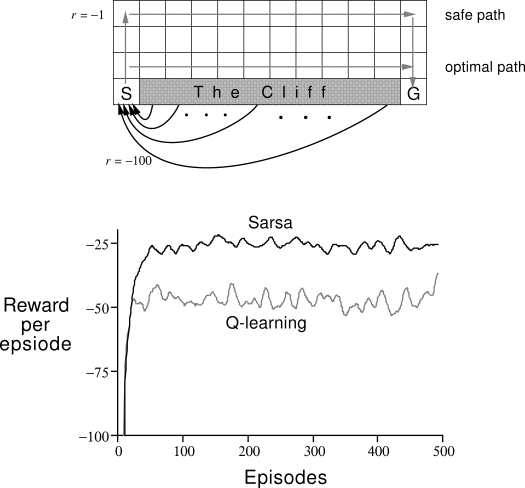
\includegraphics[width=0.7\textwidth]{cliffwalk_graph.png}
        \caption{Cliffwalk environment and reference plot (smoothed)}
\end{figure}

\noindent
In your git repo you find an implementation of the \emph{Cliff
  Walking} environment. This is a standard undiscounted ($\gamma =
1$), episodic task, with start (S) and goal (G) states, and 
actions \texttt{up, down, left, right} that cause deterministic movement.
The reward is -1 for states except those in the region marked
\textit{The Cliff}. States in this region have a reward of -100; additionally the agent is instantly set back to the start state. An episode ends when
reaching the goal state and NOT when falling down the cliff.

Recall: See slide 06:12 for pseudo code of Q-Learning; it updates the Q-function using
$$
Q_\new(s,a) \gets Q_\old(s,a)
 + \a~ [r + \g \max_{a'} Q_\old(s',a') - Q_\old(s,a)] ~.$$
SARSA is exactly the same algorithm, except that it updates the Q-function with
$$Q_\new(s,a) \gets Q_\old(s,a)
 + \a~ [r + \g Q_\old(s',a') - Q_\old(s,a)] ~,$$
where $a'$ is the action actually taken by the current policy. To implement this SARSA update, you need to sample the next action $a'$ before updating the Q-function.

\begin{enumerate}
\item Implement the SARSA and Q-learning methods using the
  $\epsilon$-greedy action selection strategy with a fixed $\epsilon=
  0.1$. Choose a small learning rate $\alpha = 0.1$. Compare the
  resulting policies when greedily selecting actions based on the
  learned Q-tables.
        
  To compare the agents' online performance run them for at
  least 500 episodes and log the \textit{reward per episode} in a
  numpy array. Plot your logged data with
  \textit{episodes} as x-axis and \textit{reward per episode} as
  y-axis. Export the logged reward array for Q-Leaning and Sarsa to
  \textit{R\_ql.csv} and \textit{R\_sa.csv respectively}. See below on
  how to plot using python.
    
\item Propose a schedule that gradually reduces $\epsilon$, starting
  from $\epsilon = 1$ (e.g., multiplicative).  Then redo question 1
  using your schedule for $\epsilon$ instead of the fixed value. Again
  plot the learning graph and export your logged rewards per episode
  to \textit{R\_ql\_sched.csv} and \textit{R\_sa\_sched.csv}
  respectively.

\item {} [Note: this doesn't make much sense: model-free RL has to fully relearn the Q-function when the reward function changes. Model-based RL would make sense. Or perhaps using a replay buffer.] In the lectures we introduced Rmax, which is a
  \emph{model-based} approach. Here we consider a simplified
  model-free Rmax-variant working with Q-Learning: Implement standard
  Q-learning using greedy action selection but a modified reward
  function. The modified reward function assigns $r_{max} = 0$ to
  unknown states ($\#(s,a)<100$) and the original reward for known
  states. Plot and export your rewards per episode
  to \textit{R\_rmax.csv}.
\end{enumerate}

{\bf
Be sure to upload your code and all your csv files containing the
rewards per episode. The evaluation is based on these files.

For each exercise get an understanding for the agent's online
behavior and their learned policies. Be ready to explain in class!

}

%\subsection{How to plot and export}

The following example shows how to plot and export data contained in a
numpy array. This is all you need to
create the plots and generate the csv files for the above exercises.

\begin{shaded}
\begin{verbatim}
import numpy as np
import matplotlib.pyplot as plt

Y = np.array([5, 8, 1, 4])

# Export to CSV
np.savetxt(Y, 'Y.csv')

# Plot and display
plt.plot(Y)
plt.show()
\end{verbatim}
\end{shaded}

Note: The graph may be very spiky so it might be a good idea to smooth your plot before comparing it with the graph given above, e.g. by using the simple box filter provided in the code. However you have to export and hand in the un-smoothed version.

%%%%%%%%%%%%%%%%%%%%%%%%%%%%%%%%%%%%%%%%%%%%%%%%%%%%%%%%%%%%%%%%%%%%%%%%%%%%%%%%

\exsection{Votieraufgabe: ~ Eligibilities in TD-learning}

Consider TD-learning in the same maze as in the previous exercise 1
(Value Iteration), where the agent starts in state $4$, and action
outcomes are probabilistic.
\begin{itemize}
\item Describe at what events plain TD-learning
will update the value function, how it will update it.
\item Assuming the
agent always decides for the clock-wise action (but outcomes are probabilistic), guess roughly how many steps
the agent will have taken when for the first time $V(s_4)$ becomes
non-zero.
\item How would this be different for eligibility traces?
\end{itemize}


%%%%%%%%%%%%%%%%%%%%%%%%%%%%%%%%%%%%%%%%%%%%%%%%%%%%%%%%%%%%%%%%%%%%%%%%%%%%%%%%

\exerfoot

\providecommand{\slides}{
  \newcommand{\slideshead}{
  \newcommand{\thepage}{\arabic{mypage}}
  %beamer
%  \documentclass[t,hyperref={bookmarks=true}]{beamer}
%  \geometry{papersize={171mm,96mm}}
  \documentclass[t,hyperref={bookmarks=true},aspectratio=169]{beamer}
  \setbeamersize{text margin left=5mm}
  \setbeamersize{text margin right=5mm}
  \usetheme{default}
  \usefonttheme[onlymath]{serif}
  \setbeamertemplate{navigation symbols}{}
  \setbeamertemplate{itemize items}{{\color{black}$\bullet$}}

  \newwrite\keyfile

  %\usepackage{palatino}
  \stdpackages
  %\usepackage{tikz} \usetikzlibrary {shapes.geometric} 
  \usepackage{multimedia}
  \usepackage[utf8]{inputenc}

  \hypersetup{
    colorlinks,
    linkcolor={blue!80!black},
    citecolor={blue!80!black},
    urlcolor={blue!80!black}
  }

  %%% geometry/spacing issues
  %\renewcommand{\baselinestretch}{1.1}
  \renewcommand{\arraystretch}{1.2}
  \columnsep 0mm

  \columnseprule 0pt
  \parindent 0ex
  \parskip 0ex
  %\setlength{\itemparsep}{3ex}
  %\renewcommand{\labelitemi}{\rule[3pt]{10pt}{10pt}~}
  %\renewcommand{\labelenumi}{\textbf{(\arabic{enumi})}}
  \setbeamertemplate{enumerate item}{(\roman{enumi})}
  \newcommand{\headerfont}{\helvetica{14}{1.5}{b}{n}}
  \newcommand{\slidefont} {\helvetica{11}{1.4}{m}{n}}
  %\newcommand{\codefont} {\helvetica{8}{1.2}{m}{n}}
  \newcommand{\urlfont} {\fontsize{6}{1.1}\selectfont}
  \renewcommand{\small} {\helvetica{10}{1.4}{m}{n}}
  \renewcommand{\tiny} {\helvetica{8}{1.3}{m}{n}}
  \newcommand{\ttiny} {\helvetica{7}{1.3}{m}{n}}

  %%% count pages properly and put the page number in bottom right
  %
  \newcounter{mypage}
  \newcommand{\incpage}{\addtocounter{mypage}{1}\setcounter{page}{\arabic{mypage}}}
  \setcounter{mypage}{0}
  \resetcounteronoverlays{page}

  \pagestyle{fancy}
  %\setlength{\headsep}{10mm}
  %\addtolength{\footheight}{15mm}
  \renewcommand{\headrulewidth}{0pt} %1pt}
  \renewcommand{\footrulewidth}{0pt} %.5pt}
  \cfoot{}
  \rhead{}
  \lhead{}
  %% \lfoot{\vspace*{-3mm}\hspace*{-3mm}\helvetica{5}{1.3}{m}{n}{\texttt{github.com/MarcToussaint/AI-lectures}}}
\lfoot{}
%  \rfoot{{\tiny\textsf{AI -- \topic -- \subtopic -- \arabic{mypage}/\pageref{lastpage}}}}
  %\lfoot{\raisebox{5mm}{\tiny\textsf{\slideauthor}}}
  %\rfoot{\raisebox{5mm}{\tiny\textsf{\slidevenue{} -- \arabic{mypage}/\pageref{lastpage}}}}
  %\rfoot{~\anchor{30,12}{\tiny\textsf{\thepage/\pageref{lastpage}}}}
  %\lfoot{\small\textsf{Marc Toussaint}}
  \rfoot{\vspace*{-4.5mm}{\tiny\textsf{\color{gray}\topic\ -- \subtopic\ -- \arabic{mypage}/\pageref{lastpage}}}\hspace*{-4mm}}
%  \rfoot{\vspace*{-4.5mm}{\tiny\textsf{\color{gray}\topic\ -- \arabic{mypage}/\pageref{lastpage}}}\hspace*{-4mm}}
%  \rfoot{~\anchor{-10,12}{\tiny\textsf{\color{gray}\topic\ --  \arabic{mypage}/\pageref{lastpage}}}}
  \lfoot{\vspace*{-4.5mm}{\hspace*{-4mm}\includegraphics[height=4mm]{LIS-26-text-long}}}

  \definecolor{grey}{rgb}{.8,.8,.8}
  \definecolor{head}{rgb}{.85,.9,.9}
%  \definecolor{blue}{rgb}{.0,.0,.5}
%  \definecolor{green}{rgb}{.0,.5,.0}
  \definecolor{red}{rgb}{.8,.0,.0}
  \definecolor{citcol}{gray}{.6}
  \newcommand{\inverted}{
    \definecolor{main}{rgb}{1,1,1}
    \color{main}
    \pagecolor[rgb]{.3,.3,.3}
  }
  \input{../latex/macros}

  \graphicspath{{pics/}{../pics/}{pics-local/}}
}

\newcommand{\slidestitle}{
  \title{\course \topic}
  \author{Marc Toussaint}
  \institute{Learning \& Intelligent Systems Lab, TU Berlin}

  \begin{document}


  %% title slide!
  \slide{}{
    \thispagestyle{empty}

    \twocol{.35}{.55}{
      %\vspace*{-5mm}%
      \hspace*{-5mm}%
      \includegraphics[width=1.\columnwidth]{\coursepicture}
    }{\center

      \textbf{\fontsize{17}{20}\selectfont \course}

      ~

      %Lecture
      \topic\\

      \vspace{1cm}

      {\tiny~\emph{\keywords}~\\}

      \vspace{1cm}

      \teacher
      
      Technical University of Berlin

      \coursedate

      ~

    }
  }
}

\newcommand{\slide}[2]{
  \slidefont
  \incpage\begin{frame}
  \addcontentsline{toc}{section}{#1}
  \vfill
  {\headerfont #1} \vspace*{-2ex}
  \begin{itemize}\item[]~\\
    #2
  \end{itemize}
  \vfill
  \end{frame}
}

% use \begin{frame}[fragile] around slidecore!
\newenvironment{slidecore}[1]{
  \slidefont\incpage
  \addcontentsline{toc}{section}{#1}
  \vfill
  {\headerfont #1} \vspace*{-2ex}
  \begin{itemize}\item[]~\\
}{
  \end{itemize}
  \vfill
}

\newcommand{\titleslide}[4][Marc Toussaint]{
  \newcommand{\slideauthor}{#1}
  \newcommand{\slidevenue}{#3}
  \slidefont
  \incpage
  \begin{frame}
  \begin{center}
    \vspace*{15mm}

    {\headerfont #2\\}
        
    \vspace*{10mm}

    #1 \\

    \vspace*{5mm}

    {\small
      Learning \& Intelligent Systems Lab, TU Berlin\\
%      Science of Intelligence Cluster of Excellence, Berlin\\
      Max Planck Fellow, Institute for Intelligent Systems\\ %Physical Reasoning \& Manipulation Lab -- 
%      MIT CSAIL\\
%      mtoussai@mit.edu,~ marc.toussaint@informatik.uni-stuttgart.de

      \vspace*{10mm}

      \emph{#3}
    }

    \vspace*{0mm}

    %\includegraphics[scale=.1]{pics/eushield-fullcolour}

  \end{center}
  \begin{itemize}\item[]~\\
    #4
  \end{itemize}
  \end{frame}
}

\newcommand{\titleslideempty}[2]{
  \slidefont
  \incpage
  \begin{frame}
  \begin{center}
    \vspace*{15mm}

    {\headerfont #1\\}
        
    %% \vspace*{5mm}

    %% {\small\emph{#2}} \\

  \end{center}
  \begin{itemize}\item[]~\\
    #2
  \end{itemize}
  \end{frame}
}

\providecommand{\key}[1]{
  \addtocounter{mypage}{1}
% \immediate\write\keyfile{#1}
  \addtocontents{toc}{\hyperref[key:#1]{#1 (\arabic{mypage})}}
%  \phantomsection\label{key:#1}
%  \index{#1@{\hyperref[key:#1]{#1 (\arabic{mysec}:\arabic{mypage})}}|phantom}
  \addtocounter{mypage}{-1}
}

\providecommand{\course}{}

\providecommand{\subtopic}{}

\providecommand{\sublecture}[2]{
  \renewcommand{\subtopic}{#1}
  \slide{#1}{#2}
}

\providecommand{\sublectureHide}[2]{
  \renewcommand{\subtopic}{#1}
}

\providecommand{\story}[1]{
~

Motivation: {\tiny #1}\clearpage
}

\newenvironment{items}[1][9]{
\par\setlength{\unitlength}{1pt}\fontsize{#1}{#1}\linespread{1.2}\selectfont
\begin{list}{--}{\leftmargin4ex \rightmargin0ex \labelsep1ex \labelwidth2ex
\topsep.7ex \parsep0ex \itemsep3pt}
}{
\end{list}
}

\newenvironment{itemS}[1][4ex]{
\par
\tiny
\begin{list}{--}{\leftmargin#1 \rightmargin0ex \labelsep1ex
  \labelwidth2ex \topsep0pt \parsep0ex \itemsep2pt}
}{
\end{list}
}

\providecommand{\slidesfoot}{
  \end{document}
}


  \slideshead
  \lecturetitleslide
}

\providecommand{\exercises}{
  \newcommand{\exerciseshead}{
  \documentclass[10pt,fleqn]{article}
  \stdpackages
\usepackage[utf8]{inputenc}

  \definecolor{bluecol}{rgb}{0,0,.5}
  \definecolor{greencol}{rgb}{0,.4,0}
  \definecolor{shadecolor}{gray}{0.9}
  \usepackage[
    %    pdftex%,
    %%    letterpaper,
    %    bookmarks,
    %    bookmarksnumbered,
    colorlinks,
    urlcolor=bluecol,
    citecolor=black,
    linkcolor=bluecol,
    %    pagecolor=bluecol,
    pdfborder={0 0 0},
    %pdfborderstyle={/S/U/W 1},
    %%    backref,     %link from bibliography back to sections
    %%    pagebackref, %link from bibliography back to pages
    %%    pdfstartview=FitH, %fitwidth instead of fit window
    pdfpagemode=UseNone, %UseOutlines, %bookmarks are displayed by acrobat
    pdftitle={\course},
    pdfauthor={Marc Toussaint},
    pdfkeywords={}
  ]{hyperref}
  \DeclareGraphicsExtensions{.pdf,.png,.jpg,.eps}

  \renewcommand{\r}{\varrho}
  \renewcommand{\l}{\lambda}
  \renewcommand{\L}{\Lambda}
  \renewcommand{\b}{\beta}
  \renewcommand{\d}{\delta}
  \renewcommand{\k}{\kappa}
  \renewcommand{\t}{\theta}
  \renewcommand{\O}{\Omega}
  \renewcommand{\o}{\omega}
  \renewcommand{\SS}{{\cal S}}
  \renewcommand{\=}{\!=\!}
  %\renewcommand{\boldsymbol}{}
  %\renewcommand{\Chapter}{\chapter}
  %\renewcommand{\Subsection}{\subsection}

  \renewcommand{\baselinestretch}{1.1}
  \geometry{a4paper,headsep=7mm,hdivide={15mm,*,15mm},vdivide={20mm,*,15mm}}

  \fancyhead[L]{\thetitle, \textit{\teacher}---\coursedate}
  \fancyhead[R]{\thepage}
  \fancyhead[C]{}
  \fancyfoot{}
  \pagestyle{fancy}

  \renewcommand{\labelenumi}{{\alph{enumi})}}

  \parindent 0pt
  \parskip 0.5ex

  \newcommand{\codefont}{\helvetica{8}{1.2}{m}{n}}
  \newcommand{\urlfont} {\fontsize{6}{1.1}\selectfont}
  \newcommand{\ttiny} {\helvetica{7}{1.3}{m}{n}}

  \input{../latex/macros}

  \DefineShortVerb{\@}

  \usepackage{comment}
  \specialcomment{solution}{
    \small
    \begin{shaded}
  }{
    \end{shaded}
  }
  
  \renewcommand{\hat}{\widehat}
  \newcommand{\bbg}{{\bar{\bar g}}}
  \graphicspath{{pics/}{../pics/}}

  \mytitle{\course\\\exnum}
  \myauthor{\teacher\\ \small\addressTUB}
  \date{\coursedate}
}

%%%%%%%%%%%%%%%%%%%%%%%%%%%%%%%%%%%%%%%%%%%%%%%%%%%%%%%%%%%%%%%%%%%%%%%%%%%%%%%%

\newcommand{\exercisestitle}{  
  \begin{document}
  \maketitle
}

\newcommand{\exsection}[1]{\section{#1}}

\newcommand{\exsubsection}[1]{\subsection{#1}}

\newcommand{\exerfoot}{
  \end{document}
}

\newenvironment{items}[1][9]{
  \par\setlength{\unitlength}{1pt}\fontsize{#1}{#1}\linespread{1.2}\selectfont
  \begin{list}{--}{\leftmargin4ex \rightmargin0ex \labelsep1ex \labelwidth2ex
      \topsep0pt \parsep0ex \itemsep3pt}
}{
  \end{list}
}

  \exerciseshead
}

\providecommand{\script}{
  \newcommand{\scripthead}{
  \documentclass[9pt,fleqn,twoside]{article}
  \stdpackages

  \usepackage{makeidx}
  \makeindex

  \usepackage{thmtools}
  \definecolor{shadecolor}{gray}{0.85}
  \declaretheoremstyle[
    %headfont=\normalfont\bfseries,
    %notefont=\mdseries, notebraces={(}{)},
    %bodyfont=\normalfont,
    %postheadspace=0.5em,
    %spaceabove=6pt,
    mdframed={
      %  skipabove=8pt,
      %  skipbelow=6pt,
      hidealllines=true,
      backgroundcolor={shadecolor},
      innertopmargin=8pt,
      %  innerleftmargin=3pt,
      %  innerrightmargin=3pt
    }
  ]{shaded}
  \declaretheorem[style=shaded,within=section,name=Definition]{myDefinition}
  \declaretheorem[style=shaded,within=section,name=Theorem]{myTheorem}
  \declaretheorem[style=shaded,within=section,name=Identities]{Identities}
  \declaretheorem[style=shaded,within=section,name=Example]{myExample}

  \definecolor{grey}{rgb}{.8,.8,.8}
  \definecolor{bluecol}{rgb}{0,0,.5}
  \definecolor{greencol}{rgb}{0,.4,0}
  \definecolor{shadecolor}{gray}{0.9}
  \definecolor{citcol}{rgb}{.4,.4,.4}
  \usepackage[
    %    pdftex%,
    %%    letterpaper,
    %bookmarks,
    bookmarksnumbered,
    colorlinks,
    urlcolor=bluecol,
    citecolor=black,
    linkcolor=bluecol,
    %    pagecolor=bluecol,
    pdfborder={0 0 0},
    %pdfborderstyle={/S/U/W 1},
    %%    backref,     %link from bibliography back to sections
    %%    pagebackref, %link from bibliography back to pages
    %%    pdfstartview=FitH, %fitwidth instead of fit window
    pdfpagemode=UseOutlines, %bookmarks are displayed by acrobat
    pdftitle={\course},
    pdfauthor={Marc Toussaint},
    pdfkeywords={}
  ]{hyperref}
  \DeclareGraphicsExtensions{.pdf,.png,.jpg,.eps}

  %\usepackage{multirow}
  \usepackage{multimedia}
  %\usepackage{marginnote}
  %\setbeamercolor{background canvas}{bg=}

  \usepackage[round]{natbib}
  \bibliographystyle{abbrvnat}

  \renewcommand{\r}{\varrho}
  \renewcommand{\l}{\lambda}
  \renewcommand{\L}{\Lambda}
  \renewcommand{\b}{\beta}
  \renewcommand{\d}{\delta}
  \renewcommand{\k}{\kappa}
  \renewcommand{\t}{\theta}
  \renewcommand{\O}{\Omega}
  \renewcommand{\o}{\omega}
  \renewcommand{\SS}{{\cal S}}
  \renewcommand{\=}{\!=\!}
  %\renewcommand{\boldsymbol}{}
  %\renewcommand{\Chapter}{\chapter}
  %\renewcommand{\Subsection}{\subsection}

  \renewcommand{\baselinestretch}{1.0}
  \geometry{a5paper,headsep=6mm,hdivide={10mm,*,10mm},vdivide={13mm,*,7mm}}

  \fancyhead[OL,ER]{\course, \textit{Marc Toussaint}}
  \fancyhead[OR,EL]{\thepage}
  \fancyhead[C]{}
  \fancyfoot{}
  \pagestyle{fancy}

  \renewcommand{\labelenumi}{{(\roman{enumi})}}
  \renewcommand{\theenumi}{(\roman{enumi})} %for ref
  \parindent 0pt
  \parskip .5pc

  \columnsep 6ex

  \renewcommand{\familydefault}{\sfdefault}

  \newcommand{\headerfont}{\large}%helvetica{12}{1}{b}{n}}
  \newcommand{\slidefont} {}%\helvetica{9}{1.3}{m}{n}}
  \newcommand{\storyfont} {}
  %  \renewcommand{\small}   {\helvetica{8}{1.2}{m}{n}}
  \renewcommand{\tiny}    {\footnotesize}%helvetica{7}{1.1}{m}{n}}
  \newcommand{\ttiny} {\footnotesize}%fontsize{7}{7}\selectfont}
%  \newcommand{\codefont}{\fontsize{6}{6}\selectfont}%helvetica{8}{1.2}{m}{n}}
  \newcommand{\codefont} {\helvetica{8}{1.2}{m}{n}}

  \input{../latex/macros}

  \usepackage{comment}
  \specialcomment{solution}{
    \small
    \begin{shaded}
  }{
    \end{shaded}
  }

  \graphicspath{{pics/}{../latex/pics/}}

  \mytitle{\course\\Lecture Script}
  \myauthor{Marc Toussaint}
  \date{\coursedate}
}

%%%%%%%%%%%%%%%%%%%%%%%%%%%%%%%%%%%%%%%%%%%%%%%%%%%%%%%%%%%%%%%%%%%%%%%%%%%%%%%%

\newcommand{\scripttitle}{
  \begin{document}
  \maketitle
  %\anchor{100,10}{\includegraphics[width=4cm]{optim}}
%  \vspace*{1cm}

  \emph{This is a direct concatenation and reformatting of all lecture
    slides and exercises from this course, including indexing to help
    prepare for exams.}

  {\tableofcontents}
}

%%%%%%%%%%%%%%%%%%%%%%%%%%%%%%%%%%%%%%%%%%%%%%%%%%%%%%%%%%%%%%%%%%%%%%%%%%%%%%%%

\newcounter{mypage}
\setcounter{mypage}{0}
\newcommand{\incpage}{\addtocounter{mypage}{1}}

\newcommand{\subtopic}{}
\newcommand{\pause}{}
\newcommand{\only}[1]{#1}

\renewcommand{\slides}[1][]{
  %  \clearpage
  \subsection{\topic}
  \index{\topic}
  {\small #1}
  \setcounter{mypage}{0}
  \smallskip\nopagebreak\hrule\medskip
}

\newcommand{\slidesfoot}{
  \bigskip
}

\newcommand{\sublecture}[2]{
  \index{#1}
}

\newcommand{\key}[1]{
  \phantomsection\addcontentsline{toc}{subsubsection}{#1}
  %\subsubsection{#1}
  \index{#1}
}

\providecommand{\defn}[1]{%
  \textbf{#1}\index{#1}%
}

\newenvironment{slidecore}[1]{
  \incpage
  \subsubsection*{#1}%{\headerfont\noindent\textbf{#1}\\}%
  \vspace{-6ex}%
  \begin{list}{$\bullet$}{\leftmargin4ex \rightmargin0ex \labelsep1ex
    \labelwidth2ex \partopsep0ex \topsep0ex \parsep.5ex \parskip0ex \itemsep0pt}\item[]~\\\nopagebreak%
}{
  \end{list}\nopagebreak%
  {\hfill\tiny \textsf{\arabic{section}.\arabic{subsection}:\arabic{mypage}}}\nopagebreak%
  \smallskip\nopagebreak\hrule
}

\newcommand{\slide}[2]{
  \begin{slidecore}{#1}
    #2
  \end{slidecore}
}

\renewcommand{\exercises}{}
\newcommand{\exercisestitle}{}
\newcommand{\exsection}[1]{\subsubsection{#1}}
\newcommand{\exerfoot}{\bigskip}

\newcommand{\story}[1]{
  \subsection*{Motivation \& Outline}
  {\storyfont\sf #1}
  \medskip\nopagebreak\hrule
}

\newcounter{savedsection}
\newcommand{\subappendix}{\setcounter{savedsection}{\arabic{section}}\appendix}
\newcommand{\noappendix}{
  \setcounter{section}{\arabic{savedsection}}% restore section number
  \setcounter{subsection}{0}% reset section counter
%  \gdef\@chapapp{\sectionname}% reset section name
  \renewcommand{\thesection}{\arabic{section}}% make section numbers arabic
}

\newenvironment{items}[1][9]{
\par\setlength{\unitlength}{1pt}\fontsize{#1}{#1}\linespread{1.2}\selectfont
\begin{list}{--}{\leftmargin4ex \rightmargin0ex \labelsep1ex \labelwidth2ex
\topsep0pt \parsep0ex \itemsep3pt}
}{
\end{list}
}

\newcommand{\Def}[1]{%
\textbf{#1}\index{#1}}%\marginnote{#1}}

  \scripthead
}

\providecommand{\note}{
  \providecommand{\notehead}[2]{
  \documentclass[#1,fleqn,twoside]{article}
  \stdpackages
  \renewcommand{\labelenumi}{{(\roman{enumi})}}
  \renewcommand{\theenumi}{(\roman{enumi})} %for ref

  \renewcommand{\baselinestretch}{#2}
  \renewcommand{\arraystretch}{1.2}
  \renewcommand{\topfraction}{1}
  \renewcommand{\bottomfraction}{1}
  \renewcommand{\textfraction}{0}
  \columnsep 5ex
  \parindent 3ex
  \parskip 1ex

  % Lists and paragraphs
  \parindent 0pt
  \topsep 4pt plus 1pt minus 2pt
  \partopsep 1pt plus 0.5pt minus 0.5pt
  \itemsep 2pt plus 1pt minus 0.5pt
  \parsep 2pt plus 1pt minus 0.5pt
  \parskip .5pc %add _in_ {thebibliography} environment in *.bbl

  \setcounter{tocdepth}{3}
  \setcounter{secnumdepth}{3}

  \geometry{a4paper,hdivide={25mm,*,25mm},vdivide={25mm,*,25mm}}

  \renewcommand{\headrulewidth}{.0pt}\renewcommand{\footrulewidth}{.0pt}\cfoot{}
  \fancyhead[OL,EC]{\it\theauthor---\today}
  \fancyhead[ER]{\leftmark}
  \fancyhead[OR,EL]{\thepage}
  \fancyfoot[EL,OR]{}
  \setlength{\headsep}{10mm}
  %\fancyhead[OL]{\rightmark}
  %\fancyfoot[EL,OR]{}


  %  \usepackage{palatino}

  \newcommand{\codefont}{\helvetica{8}{1.2}{m}{n}}

  \renewenvironment{abstract}{
    \vspace*{5ex}\begin{list}{}{
      \leftmargin3ex
      \rightmargin3ex
      \topsep-\parskip}\item[]
     \hrule\vspace{1.5ex}{\bf Abstract.~}\small}
    {\vspace{2ex}\hrule\end{list}\vspace{5ex}}
    
  \newenvironment{keyword}
    {\par{\it Keywords:~}}
    {}

  \def\makemytitle{%
    \thispagestyle{empty}
    \begin{list}{}{\leftmargin3ex \rightmargin3ex \topsep0ex \parsep0ex}\item[]
      \begin{center}
        {\fontsize{18}{25}\selectfont{\thetitle\\}}\vspace{5ex}

        {\fontsize{14}{16}\selectfont{\theauthor\\}}\vspace{1ex}

        {\footnotesize{\sl \addressFUB}\\ \emailBerlin}

        {\footnotesize \today}

        \vspace{1ex}
        {\small \published}
      \end{center}
    \end{list}
    \renewcommand{\maketitle}{\chapter{\thetitle}}
  }

  \input{../latex/macros}
  \pdflatex

  \graphicspath{{pics/}{../pics/}{pics-local/}}

  \myauthor{Marc Toussaint}
  \date{\today}
}

%%%%%%%%%%%%%%%%%%%%%%%%%%%%%%%%%%%%%%%%%%%%%%%%%%%%%%%%%%%%%%%%%%%%%%%%%%%%%%%%

\newcommand{\notetitle}{
  \begin{document}
  \thispagestyle{empty}
    
  \maketitle

}

\newenvironment{items}[1][9]{
\par\setlength{\unitlength}{1pt}\fontsize{#1}{#1}\linespread{1.2}\selectfont
\begin{list}{--}{\leftmargin4ex \rightmargin0ex \labelsep1ex \labelwidth2ex
\topsep0pt \parsep0ex \itemsep3pt}
}{
\end{list}
}

  \notehead{10}{1.1}
}

\providecommand{\course}{NO COURSE}
\providecommand{\coursepicture}{NO PICTURE}
\providecommand{\coursedate}{NO DATE}
\providecommand{\topic}{NO TOPIC}
\providecommand{\keywords}{NO KEYWORDS}
\providecommand{\exnum}{NO NUMBER}
\providecommand{\teacher}{Marc Toussaint}

\providecommand{\stdpackages}{
  \usepackage{amsmath}
  \usepackage{amssymb}
  \usepackage{amsfonts}
  \allowdisplaybreaks
  \usepackage{amsthm}
  \usepackage{eucal}
  \usepackage{graphicx}
  \usepackage{color}
  \usepackage{geometry}
  \usepackage{framed}
%  \usecolor{xcolor}
  \definecolor{shadecolor}{gray}{0.9}
  \setlength{\FrameSep}{3pt}
  \usepackage{fancyvrb}
  \fvset{numbers=none,xleftmargin=5ex}

  \usepackage{pdfpages}

  \usepackage{multicol} 
  \usepackage{fancyhdr}
}

\providecommand{\addressUSTT}{
  Machine~Learning~\&~Robotics~lab, U~Stuttgart\\\small
  Universit{\"a}tsstra{\ss}e 38, 70569~Stuttgart, Germany
}

\providecommand{\addressTUB}{
  Learning~\&~Intelligent~Systems~Lab, TU~Berlin\\\small
  Marchstr. 23, 10587 Berlin, Germany
}


\renewcommand{\course}{Artificial Intelligence}
\renewcommand{\coursepicture}{course_ai}
\renewcommand{\coursedate}{Winter 2019}
\renewcommand{\exnum}{Exercise 5}

\exercises
\excludecomment{solution}
\exercisestitle

%%%%%%%%%%%%%%%%%%%%%%%%%%%%%%%%%%%%%%%%%%%%%%%%%%%%%%%%%%%%%%%%%%%%%%%%%%%%%%%%

\exsection{Programmieraufgabe:~ Constrained Satisfaction Problems}

Pull the current exercise from our server to your local repository.

\textbf{Task 1:} Implement backtracking for the constrained satisfaction problem
definition you find in @csp.py@. Make three different versions of it 1) without
any heuristic 2) with minimal remaining value as heuristic but without
tie-breaker (take the first best solution) 3) with minimal remaining value and
the degree heuristic as tie-breaker.

\textbf{Optional:} Implement AC-3 or any approximate form of
constraint propagation and activate it if the according
parameter is set.

\textbf{Task 2:} Implement a method to convert a Sudoku into a
@csp.ConstrainedSatisfactionProblem@, and then use this to solve the sudoku given as a numpy array. Every empty field is set to
@0@. The CSP you create should cover all rules of a Sudoku, which are
(from
\url{http://en.wikipedia.org/wiki/Sudoku}): 
\begin{quote}
\emph{Fill a $9 \times 9$ grid with digits so that each column, each row,
and each of the nine $3 \times 3$ sub-grids that compose the grid
(also called 'blocks') contains all of the digits from 1 to 9.}
\end{quote}
In the lecture we mentioned the \emph{all\_different} constraint for
columns, rows, and blocks. As the\\ @csp.ConstrainedSatisfactionProblem@
only allows you to represent pair-wise \emph{unequal} constraints (to
facilitate constraint propagation) you need to convert this.

~
%The blocks are depicted by the bold lines in the picture.

\begin{center}
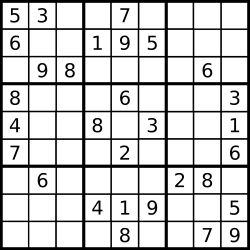
\includegraphics[width=5cm]{sudoku.png}
\end{center}

%%%%%%%%%%%%%%%%%%%%%%%%%%%%%%%%%%%%%%%%%%%%%%%%%%%%%%%%%%%%%%%%%%%%%%%%%%%%%%%%

\exsection{Votieraufgabe: ~ CSP}

Betrachten Sie folgenden Kartenausschnitt:

\show[.5]{europa-skizze-bearbeitet.png}

Der Kartenausschnitt soll mit insgesamt 4 Farben so eingef"arbt werden, dass je zwei Nachbarl"ander verschiedene Farben besitzen.

Mit welchem Land w"urde man am ehesten beginnen?

F"arben Sie das erste Land ein und wenden Sie durchgehend Constraint Propagation an.

%%%%%%%%%%%%%%%%%%%%%%%%%%%%%%%%%%%%%%%%%%%%%%%%%%%%%%%%%%%%%%%%%%%%%%%%%%%%%%%%

\exsection{Präsenzaufgabe: ~ Generalized Arc Consistency}

We have $n$ variables $x_i$, each with the (current) domain
$D_i$. Constraint propagation by establishing local constraint
consistency (``arc consistency'') in general means the following:

For a variable $x_i$ and an adjacent constraint $C_k$, we delete all
values $v$ from $D_i$ for which there exists no tuple $\tau \in D_{I_k}$
with $\tau_i=v$ that satisfies the constraint.

Consider a simple example
$$x_1,x_2 \in \{1,2\}\comma x_3, x_4 \in\{2,..,6\}\comma
c = \text{AllDiff}(x_1,..,x_4)$$

(a) How does constraint propagation from $c$ to $x_3$ update the domain $D_3$?

(b) On \url{http://norvig.com/sudoku.html} Norvig describes his Sudoku
solver, using the following rules for constraint propagation:
\begin{quote}
(1) If a square has only one possible value, then eliminate that value
from the square's peers.

(2) If a unit (block, row or column) has only one possible place for a
value, then put the value there.
\end{quote}
Is this a general implementation of constraint propagation for
the \emph{allDiff} constraint?

~

Note: The generalized arc consistency is equivalent so-called message
passing (or belief propagation) in probabilistic networks, except that
the messages are domain sets instead of belief vectors.

See also \url{www.lirmm.fr/~bessiere/stock/TR06020.pdf}



\exerfoot


\providecommand{\slides}{
  \newcommand{\slideshead}{
  \newcommand{\thepage}{\arabic{mypage}}
  %beamer
%  \documentclass[t,hyperref={bookmarks=true}]{beamer}
%  \geometry{papersize={171mm,96mm}}
  \documentclass[t,hyperref={bookmarks=true},aspectratio=169]{beamer}
  \setbeamersize{text margin left=5mm}
  \setbeamersize{text margin right=5mm}
  \usetheme{default}
  \usefonttheme[onlymath]{serif}
  \setbeamertemplate{navigation symbols}{}
  \setbeamertemplate{itemize items}{{\color{black}$\bullet$}}

  \newwrite\keyfile

  %\usepackage{palatino}
  \stdpackages
  %\usepackage{tikz} \usetikzlibrary {shapes.geometric} 
  \usepackage{multimedia}
  \usepackage[utf8]{inputenc}

  \hypersetup{
    colorlinks,
    linkcolor={blue!80!black},
    citecolor={blue!80!black},
    urlcolor={blue!80!black}
  }

  %%% geometry/spacing issues
  %\renewcommand{\baselinestretch}{1.1}
  \renewcommand{\arraystretch}{1.2}
  \columnsep 0mm

  \columnseprule 0pt
  \parindent 0ex
  \parskip 0ex
  %\setlength{\itemparsep}{3ex}
  %\renewcommand{\labelitemi}{\rule[3pt]{10pt}{10pt}~}
  %\renewcommand{\labelenumi}{\textbf{(\arabic{enumi})}}
  \setbeamertemplate{enumerate item}{(\roman{enumi})}
  \newcommand{\headerfont}{\helvetica{14}{1.5}{b}{n}}
  \newcommand{\slidefont} {\helvetica{11}{1.4}{m}{n}}
  %\newcommand{\codefont} {\helvetica{8}{1.2}{m}{n}}
  \newcommand{\urlfont} {\fontsize{6}{1.1}\selectfont}
  \renewcommand{\small} {\helvetica{10}{1.4}{m}{n}}
  \renewcommand{\tiny} {\helvetica{8}{1.3}{m}{n}}
  \newcommand{\ttiny} {\helvetica{7}{1.3}{m}{n}}

  %%% count pages properly and put the page number in bottom right
  %
  \newcounter{mypage}
  \newcommand{\incpage}{\addtocounter{mypage}{1}\setcounter{page}{\arabic{mypage}}}
  \setcounter{mypage}{0}
  \resetcounteronoverlays{page}

  \pagestyle{fancy}
  %\setlength{\headsep}{10mm}
  %\addtolength{\footheight}{15mm}
  \renewcommand{\headrulewidth}{0pt} %1pt}
  \renewcommand{\footrulewidth}{0pt} %.5pt}
  \cfoot{}
  \rhead{}
  \lhead{}
  %% \lfoot{\vspace*{-3mm}\hspace*{-3mm}\helvetica{5}{1.3}{m}{n}{\texttt{github.com/MarcToussaint/AI-lectures}}}
\lfoot{}
%  \rfoot{{\tiny\textsf{AI -- \topic -- \subtopic -- \arabic{mypage}/\pageref{lastpage}}}}
  %\lfoot{\raisebox{5mm}{\tiny\textsf{\slideauthor}}}
  %\rfoot{\raisebox{5mm}{\tiny\textsf{\slidevenue{} -- \arabic{mypage}/\pageref{lastpage}}}}
  %\rfoot{~\anchor{30,12}{\tiny\textsf{\thepage/\pageref{lastpage}}}}
  %\lfoot{\small\textsf{Marc Toussaint}}
  \rfoot{\vspace*{-4.5mm}{\tiny\textsf{\color{gray}\topic\ -- \subtopic\ -- \arabic{mypage}/\pageref{lastpage}}}\hspace*{-4mm}}
%  \rfoot{\vspace*{-4.5mm}{\tiny\textsf{\color{gray}\topic\ -- \arabic{mypage}/\pageref{lastpage}}}\hspace*{-4mm}}
%  \rfoot{~\anchor{-10,12}{\tiny\textsf{\color{gray}\topic\ --  \arabic{mypage}/\pageref{lastpage}}}}
  \lfoot{\vspace*{-4.5mm}{\hspace*{-4mm}\includegraphics[height=4mm]{LIS-26-text-long}}}

  \definecolor{grey}{rgb}{.8,.8,.8}
  \definecolor{head}{rgb}{.85,.9,.9}
%  \definecolor{blue}{rgb}{.0,.0,.5}
%  \definecolor{green}{rgb}{.0,.5,.0}
  \definecolor{red}{rgb}{.8,.0,.0}
  \definecolor{citcol}{gray}{.6}
  \newcommand{\inverted}{
    \definecolor{main}{rgb}{1,1,1}
    \color{main}
    \pagecolor[rgb]{.3,.3,.3}
  }
  \input{../latex/macros}

  \graphicspath{{pics/}{../pics/}{pics-local/}}
}

\newcommand{\slidestitle}{
  \title{\course \topic}
  \author{Marc Toussaint}
  \institute{Learning \& Intelligent Systems Lab, TU Berlin}

  \begin{document}


  %% title slide!
  \slide{}{
    \thispagestyle{empty}

    \twocol{.35}{.55}{
      %\vspace*{-5mm}%
      \hspace*{-5mm}%
      \includegraphics[width=1.\columnwidth]{\coursepicture}
    }{\center

      \textbf{\fontsize{17}{20}\selectfont \course}

      ~

      %Lecture
      \topic\\

      \vspace{1cm}

      {\tiny~\emph{\keywords}~\\}

      \vspace{1cm}

      \teacher
      
      Technical University of Berlin

      \coursedate

      ~

    }
  }
}

\newcommand{\slide}[2]{
  \slidefont
  \incpage\begin{frame}
  \addcontentsline{toc}{section}{#1}
  \vfill
  {\headerfont #1} \vspace*{-2ex}
  \begin{itemize}\item[]~\\
    #2
  \end{itemize}
  \vfill
  \end{frame}
}

% use \begin{frame}[fragile] around slidecore!
\newenvironment{slidecore}[1]{
  \slidefont\incpage
  \addcontentsline{toc}{section}{#1}
  \vfill
  {\headerfont #1} \vspace*{-2ex}
  \begin{itemize}\item[]~\\
}{
  \end{itemize}
  \vfill
}

\newcommand{\titleslide}[4][Marc Toussaint]{
  \newcommand{\slideauthor}{#1}
  \newcommand{\slidevenue}{#3}
  \slidefont
  \incpage
  \begin{frame}
  \begin{center}
    \vspace*{15mm}

    {\headerfont #2\\}
        
    \vspace*{10mm}

    #1 \\

    \vspace*{5mm}

    {\small
      Learning \& Intelligent Systems Lab, TU Berlin\\
%      Science of Intelligence Cluster of Excellence, Berlin\\
      Max Planck Fellow, Institute for Intelligent Systems\\ %Physical Reasoning \& Manipulation Lab -- 
%      MIT CSAIL\\
%      mtoussai@mit.edu,~ marc.toussaint@informatik.uni-stuttgart.de

      \vspace*{10mm}

      \emph{#3}
    }

    \vspace*{0mm}

    %\includegraphics[scale=.1]{pics/eushield-fullcolour}

  \end{center}
  \begin{itemize}\item[]~\\
    #4
  \end{itemize}
  \end{frame}
}

\newcommand{\titleslideempty}[2]{
  \slidefont
  \incpage
  \begin{frame}
  \begin{center}
    \vspace*{15mm}

    {\headerfont #1\\}
        
    %% \vspace*{5mm}

    %% {\small\emph{#2}} \\

  \end{center}
  \begin{itemize}\item[]~\\
    #2
  \end{itemize}
  \end{frame}
}

\providecommand{\key}[1]{
  \addtocounter{mypage}{1}
% \immediate\write\keyfile{#1}
  \addtocontents{toc}{\hyperref[key:#1]{#1 (\arabic{mypage})}}
%  \phantomsection\label{key:#1}
%  \index{#1@{\hyperref[key:#1]{#1 (\arabic{mysec}:\arabic{mypage})}}|phantom}
  \addtocounter{mypage}{-1}
}

\providecommand{\course}{}

\providecommand{\subtopic}{}

\providecommand{\sublecture}[2]{
  \renewcommand{\subtopic}{#1}
  \slide{#1}{#2}
}

\providecommand{\sublectureHide}[2]{
  \renewcommand{\subtopic}{#1}
}

\providecommand{\story}[1]{
~

Motivation: {\tiny #1}\clearpage
}

\newenvironment{items}[1][9]{
\par\setlength{\unitlength}{1pt}\fontsize{#1}{#1}\linespread{1.2}\selectfont
\begin{list}{--}{\leftmargin4ex \rightmargin0ex \labelsep1ex \labelwidth2ex
\topsep.7ex \parsep0ex \itemsep3pt}
}{
\end{list}
}

\newenvironment{itemS}[1][4ex]{
\par
\tiny
\begin{list}{--}{\leftmargin#1 \rightmargin0ex \labelsep1ex
  \labelwidth2ex \topsep0pt \parsep0ex \itemsep2pt}
}{
\end{list}
}

\providecommand{\slidesfoot}{
  \end{document}
}


  \slideshead
  \lecturetitleslide
}

\providecommand{\exercises}{
  \newcommand{\exerciseshead}{
  \documentclass[10pt,fleqn]{article}
  \stdpackages
\usepackage[utf8]{inputenc}

  \definecolor{bluecol}{rgb}{0,0,.5}
  \definecolor{greencol}{rgb}{0,.4,0}
  \definecolor{shadecolor}{gray}{0.9}
  \usepackage[
    %    pdftex%,
    %%    letterpaper,
    %    bookmarks,
    %    bookmarksnumbered,
    colorlinks,
    urlcolor=bluecol,
    citecolor=black,
    linkcolor=bluecol,
    %    pagecolor=bluecol,
    pdfborder={0 0 0},
    %pdfborderstyle={/S/U/W 1},
    %%    backref,     %link from bibliography back to sections
    %%    pagebackref, %link from bibliography back to pages
    %%    pdfstartview=FitH, %fitwidth instead of fit window
    pdfpagemode=UseNone, %UseOutlines, %bookmarks are displayed by acrobat
    pdftitle={\course},
    pdfauthor={Marc Toussaint},
    pdfkeywords={}
  ]{hyperref}
  \DeclareGraphicsExtensions{.pdf,.png,.jpg,.eps}

  \renewcommand{\r}{\varrho}
  \renewcommand{\l}{\lambda}
  \renewcommand{\L}{\Lambda}
  \renewcommand{\b}{\beta}
  \renewcommand{\d}{\delta}
  \renewcommand{\k}{\kappa}
  \renewcommand{\t}{\theta}
  \renewcommand{\O}{\Omega}
  \renewcommand{\o}{\omega}
  \renewcommand{\SS}{{\cal S}}
  \renewcommand{\=}{\!=\!}
  %\renewcommand{\boldsymbol}{}
  %\renewcommand{\Chapter}{\chapter}
  %\renewcommand{\Subsection}{\subsection}

  \renewcommand{\baselinestretch}{1.1}
  \geometry{a4paper,headsep=7mm,hdivide={15mm,*,15mm},vdivide={20mm,*,15mm}}

  \fancyhead[L]{\thetitle, \textit{\teacher}---\coursedate}
  \fancyhead[R]{\thepage}
  \fancyhead[C]{}
  \fancyfoot{}
  \pagestyle{fancy}

  \renewcommand{\labelenumi}{{\alph{enumi})}}

  \parindent 0pt
  \parskip 0.5ex

  \newcommand{\codefont}{\helvetica{8}{1.2}{m}{n}}
  \newcommand{\urlfont} {\fontsize{6}{1.1}\selectfont}
  \newcommand{\ttiny} {\helvetica{7}{1.3}{m}{n}}

  \input{../latex/macros}

  \DefineShortVerb{\@}

  \usepackage{comment}
  \specialcomment{solution}{
    \small
    \begin{shaded}
  }{
    \end{shaded}
  }
  
  \renewcommand{\hat}{\widehat}
  \newcommand{\bbg}{{\bar{\bar g}}}
  \graphicspath{{pics/}{../pics/}}

  \mytitle{\course\\\exnum}
  \myauthor{\teacher\\ \small\addressTUB}
  \date{\coursedate}
}

%%%%%%%%%%%%%%%%%%%%%%%%%%%%%%%%%%%%%%%%%%%%%%%%%%%%%%%%%%%%%%%%%%%%%%%%%%%%%%%%

\newcommand{\exercisestitle}{  
  \begin{document}
  \maketitle
}

\newcommand{\exsection}[1]{\section{#1}}

\newcommand{\exsubsection}[1]{\subsection{#1}}

\newcommand{\exerfoot}{
  \end{document}
}

\newenvironment{items}[1][9]{
  \par\setlength{\unitlength}{1pt}\fontsize{#1}{#1}\linespread{1.2}\selectfont
  \begin{list}{--}{\leftmargin4ex \rightmargin0ex \labelsep1ex \labelwidth2ex
      \topsep0pt \parsep0ex \itemsep3pt}
}{
  \end{list}
}

  \exerciseshead
}

\providecommand{\script}{
  \newcommand{\scripthead}{
  \documentclass[9pt,fleqn,twoside]{article}
  \stdpackages

  \usepackage{makeidx}
  \makeindex

  \usepackage{thmtools}
  \definecolor{shadecolor}{gray}{0.85}
  \declaretheoremstyle[
    %headfont=\normalfont\bfseries,
    %notefont=\mdseries, notebraces={(}{)},
    %bodyfont=\normalfont,
    %postheadspace=0.5em,
    %spaceabove=6pt,
    mdframed={
      %  skipabove=8pt,
      %  skipbelow=6pt,
      hidealllines=true,
      backgroundcolor={shadecolor},
      innertopmargin=8pt,
      %  innerleftmargin=3pt,
      %  innerrightmargin=3pt
    }
  ]{shaded}
  \declaretheorem[style=shaded,within=section,name=Definition]{myDefinition}
  \declaretheorem[style=shaded,within=section,name=Theorem]{myTheorem}
  \declaretheorem[style=shaded,within=section,name=Identities]{Identities}
  \declaretheorem[style=shaded,within=section,name=Example]{myExample}

  \definecolor{grey}{rgb}{.8,.8,.8}
  \definecolor{bluecol}{rgb}{0,0,.5}
  \definecolor{greencol}{rgb}{0,.4,0}
  \definecolor{shadecolor}{gray}{0.9}
  \definecolor{citcol}{rgb}{.4,.4,.4}
  \usepackage[
    %    pdftex%,
    %%    letterpaper,
    %bookmarks,
    bookmarksnumbered,
    colorlinks,
    urlcolor=bluecol,
    citecolor=black,
    linkcolor=bluecol,
    %    pagecolor=bluecol,
    pdfborder={0 0 0},
    %pdfborderstyle={/S/U/W 1},
    %%    backref,     %link from bibliography back to sections
    %%    pagebackref, %link from bibliography back to pages
    %%    pdfstartview=FitH, %fitwidth instead of fit window
    pdfpagemode=UseOutlines, %bookmarks are displayed by acrobat
    pdftitle={\course},
    pdfauthor={Marc Toussaint},
    pdfkeywords={}
  ]{hyperref}
  \DeclareGraphicsExtensions{.pdf,.png,.jpg,.eps}

  %\usepackage{multirow}
  \usepackage{multimedia}
  %\usepackage{marginnote}
  %\setbeamercolor{background canvas}{bg=}

  \usepackage[round]{natbib}
  \bibliographystyle{abbrvnat}

  \renewcommand{\r}{\varrho}
  \renewcommand{\l}{\lambda}
  \renewcommand{\L}{\Lambda}
  \renewcommand{\b}{\beta}
  \renewcommand{\d}{\delta}
  \renewcommand{\k}{\kappa}
  \renewcommand{\t}{\theta}
  \renewcommand{\O}{\Omega}
  \renewcommand{\o}{\omega}
  \renewcommand{\SS}{{\cal S}}
  \renewcommand{\=}{\!=\!}
  %\renewcommand{\boldsymbol}{}
  %\renewcommand{\Chapter}{\chapter}
  %\renewcommand{\Subsection}{\subsection}

  \renewcommand{\baselinestretch}{1.0}
  \geometry{a5paper,headsep=6mm,hdivide={10mm,*,10mm},vdivide={13mm,*,7mm}}

  \fancyhead[OL,ER]{\course, \textit{Marc Toussaint}}
  \fancyhead[OR,EL]{\thepage}
  \fancyhead[C]{}
  \fancyfoot{}
  \pagestyle{fancy}

  \renewcommand{\labelenumi}{{(\roman{enumi})}}
  \renewcommand{\theenumi}{(\roman{enumi})} %for ref
  \parindent 0pt
  \parskip .5pc

  \columnsep 6ex

  \renewcommand{\familydefault}{\sfdefault}

  \newcommand{\headerfont}{\large}%helvetica{12}{1}{b}{n}}
  \newcommand{\slidefont} {}%\helvetica{9}{1.3}{m}{n}}
  \newcommand{\storyfont} {}
  %  \renewcommand{\small}   {\helvetica{8}{1.2}{m}{n}}
  \renewcommand{\tiny}    {\footnotesize}%helvetica{7}{1.1}{m}{n}}
  \newcommand{\ttiny} {\footnotesize}%fontsize{7}{7}\selectfont}
%  \newcommand{\codefont}{\fontsize{6}{6}\selectfont}%helvetica{8}{1.2}{m}{n}}
  \newcommand{\codefont} {\helvetica{8}{1.2}{m}{n}}

  \input{../latex/macros}

  \usepackage{comment}
  \specialcomment{solution}{
    \small
    \begin{shaded}
  }{
    \end{shaded}
  }

  \graphicspath{{pics/}{../latex/pics/}}

  \mytitle{\course\\Lecture Script}
  \myauthor{Marc Toussaint}
  \date{\coursedate}
}

%%%%%%%%%%%%%%%%%%%%%%%%%%%%%%%%%%%%%%%%%%%%%%%%%%%%%%%%%%%%%%%%%%%%%%%%%%%%%%%%

\newcommand{\scripttitle}{
  \begin{document}
  \maketitle
  %\anchor{100,10}{\includegraphics[width=4cm]{optim}}
%  \vspace*{1cm}

  \emph{This is a direct concatenation and reformatting of all lecture
    slides and exercises from this course, including indexing to help
    prepare for exams.}

  {\tableofcontents}
}

%%%%%%%%%%%%%%%%%%%%%%%%%%%%%%%%%%%%%%%%%%%%%%%%%%%%%%%%%%%%%%%%%%%%%%%%%%%%%%%%

\newcounter{mypage}
\setcounter{mypage}{0}
\newcommand{\incpage}{\addtocounter{mypage}{1}}

\newcommand{\subtopic}{}
\newcommand{\pause}{}
\newcommand{\only}[1]{#1}

\renewcommand{\slides}[1][]{
  %  \clearpage
  \subsection{\topic}
  \index{\topic}
  {\small #1}
  \setcounter{mypage}{0}
  \smallskip\nopagebreak\hrule\medskip
}

\newcommand{\slidesfoot}{
  \bigskip
}

\newcommand{\sublecture}[2]{
  \index{#1}
}

\newcommand{\key}[1]{
  \phantomsection\addcontentsline{toc}{subsubsection}{#1}
  %\subsubsection{#1}
  \index{#1}
}

\providecommand{\defn}[1]{%
  \textbf{#1}\index{#1}%
}

\newenvironment{slidecore}[1]{
  \incpage
  \subsubsection*{#1}%{\headerfont\noindent\textbf{#1}\\}%
  \vspace{-6ex}%
  \begin{list}{$\bullet$}{\leftmargin4ex \rightmargin0ex \labelsep1ex
    \labelwidth2ex \partopsep0ex \topsep0ex \parsep.5ex \parskip0ex \itemsep0pt}\item[]~\\\nopagebreak%
}{
  \end{list}\nopagebreak%
  {\hfill\tiny \textsf{\arabic{section}.\arabic{subsection}:\arabic{mypage}}}\nopagebreak%
  \smallskip\nopagebreak\hrule
}

\newcommand{\slide}[2]{
  \begin{slidecore}{#1}
    #2
  \end{slidecore}
}

\renewcommand{\exercises}{}
\newcommand{\exercisestitle}{}
\newcommand{\exsection}[1]{\subsubsection{#1}}
\newcommand{\exerfoot}{\bigskip}

\newcommand{\story}[1]{
  \subsection*{Motivation \& Outline}
  {\storyfont\sf #1}
  \medskip\nopagebreak\hrule
}

\newcounter{savedsection}
\newcommand{\subappendix}{\setcounter{savedsection}{\arabic{section}}\appendix}
\newcommand{\noappendix}{
  \setcounter{section}{\arabic{savedsection}}% restore section number
  \setcounter{subsection}{0}% reset section counter
%  \gdef\@chapapp{\sectionname}% reset section name
  \renewcommand{\thesection}{\arabic{section}}% make section numbers arabic
}

\newenvironment{items}[1][9]{
\par\setlength{\unitlength}{1pt}\fontsize{#1}{#1}\linespread{1.2}\selectfont
\begin{list}{--}{\leftmargin4ex \rightmargin0ex \labelsep1ex \labelwidth2ex
\topsep0pt \parsep0ex \itemsep3pt}
}{
\end{list}
}

\newcommand{\Def}[1]{%
\textbf{#1}\index{#1}}%\marginnote{#1}}

  \scripthead
}

\providecommand{\note}{
  \providecommand{\notehead}[2]{
  \documentclass[#1,fleqn,twoside]{article}
  \stdpackages
  \renewcommand{\labelenumi}{{(\roman{enumi})}}
  \renewcommand{\theenumi}{(\roman{enumi})} %for ref

  \renewcommand{\baselinestretch}{#2}
  \renewcommand{\arraystretch}{1.2}
  \renewcommand{\topfraction}{1}
  \renewcommand{\bottomfraction}{1}
  \renewcommand{\textfraction}{0}
  \columnsep 5ex
  \parindent 3ex
  \parskip 1ex

  % Lists and paragraphs
  \parindent 0pt
  \topsep 4pt plus 1pt minus 2pt
  \partopsep 1pt plus 0.5pt minus 0.5pt
  \itemsep 2pt plus 1pt minus 0.5pt
  \parsep 2pt plus 1pt minus 0.5pt
  \parskip .5pc %add _in_ {thebibliography} environment in *.bbl

  \setcounter{tocdepth}{3}
  \setcounter{secnumdepth}{3}

  \geometry{a4paper,hdivide={25mm,*,25mm},vdivide={25mm,*,25mm}}

  \renewcommand{\headrulewidth}{.0pt}\renewcommand{\footrulewidth}{.0pt}\cfoot{}
  \fancyhead[OL,EC]{\it\theauthor---\today}
  \fancyhead[ER]{\leftmark}
  \fancyhead[OR,EL]{\thepage}
  \fancyfoot[EL,OR]{}
  \setlength{\headsep}{10mm}
  %\fancyhead[OL]{\rightmark}
  %\fancyfoot[EL,OR]{}


  %  \usepackage{palatino}

  \newcommand{\codefont}{\helvetica{8}{1.2}{m}{n}}

  \renewenvironment{abstract}{
    \vspace*{5ex}\begin{list}{}{
      \leftmargin3ex
      \rightmargin3ex
      \topsep-\parskip}\item[]
     \hrule\vspace{1.5ex}{\bf Abstract.~}\small}
    {\vspace{2ex}\hrule\end{list}\vspace{5ex}}
    
  \newenvironment{keyword}
    {\par{\it Keywords:~}}
    {}

  \def\makemytitle{%
    \thispagestyle{empty}
    \begin{list}{}{\leftmargin3ex \rightmargin3ex \topsep0ex \parsep0ex}\item[]
      \begin{center}
        {\fontsize{18}{25}\selectfont{\thetitle\\}}\vspace{5ex}

        {\fontsize{14}{16}\selectfont{\theauthor\\}}\vspace{1ex}

        {\footnotesize{\sl \addressFUB}\\ \emailBerlin}

        {\footnotesize \today}

        \vspace{1ex}
        {\small \published}
      \end{center}
    \end{list}
    \renewcommand{\maketitle}{\chapter{\thetitle}}
  }

  \input{../latex/macros}
  \pdflatex

  \graphicspath{{pics/}{../pics/}{pics-local/}}

  \myauthor{Marc Toussaint}
  \date{\today}
}

%%%%%%%%%%%%%%%%%%%%%%%%%%%%%%%%%%%%%%%%%%%%%%%%%%%%%%%%%%%%%%%%%%%%%%%%%%%%%%%%

\newcommand{\notetitle}{
  \begin{document}
  \thispagestyle{empty}
    
  \maketitle

}

\newenvironment{items}[1][9]{
\par\setlength{\unitlength}{1pt}\fontsize{#1}{#1}\linespread{1.2}\selectfont
\begin{list}{--}{\leftmargin4ex \rightmargin0ex \labelsep1ex \labelwidth2ex
\topsep0pt \parsep0ex \itemsep3pt}
}{
\end{list}
}

  \notehead{10}{1.1}
}

\providecommand{\course}{NO COURSE}
\providecommand{\coursepicture}{NO PICTURE}
\providecommand{\coursedate}{NO DATE}
\providecommand{\topic}{NO TOPIC}
\providecommand{\keywords}{NO KEYWORDS}
\providecommand{\exnum}{NO NUMBER}
\providecommand{\teacher}{Marc Toussaint}

\providecommand{\stdpackages}{
  \usepackage{amsmath}
  \usepackage{amssymb}
  \usepackage{amsfonts}
  \allowdisplaybreaks
  \usepackage{amsthm}
  \usepackage{eucal}
  \usepackage{graphicx}
  \usepackage{color}
  \usepackage{geometry}
  \usepackage{framed}
%  \usecolor{xcolor}
  \definecolor{shadecolor}{gray}{0.9}
  \setlength{\FrameSep}{3pt}
  \usepackage{fancyvrb}
  \fvset{numbers=none,xleftmargin=5ex}

  \usepackage{pdfpages}

  \usepackage{multicol} 
  \usepackage{fancyhdr}
}

\providecommand{\addressUSTT}{
  Machine~Learning~\&~Robotics~lab, U~Stuttgart\\\small
  Universit{\"a}tsstra{\ss}e 38, 70569~Stuttgart, Germany
}

\providecommand{\addressTUB}{
  Learning~\&~Intelligent~Systems~Lab, TU~Berlin\\\small
  Marchstr. 23, 10587 Berlin, Germany
}


\renewcommand{\course}{Artificial Intelligence}
\renewcommand{\coursepicture}{course_ai}
\renewcommand{\coursedate}{Winter 2019}
\renewcommand{\exnum}{Exercise 6}

\exercises
\excludecomment{solution}
\exercisestitle

%%%%%%%%%%%%%%%%%%%%%%%%%%%%%%%%%%%%%%%%%%%%%%%%%%%%%%%%%%%%%%%%%%%%%%%%%%%%%%%%

\exsection{Programmieraufgabe: Spamfilter mit Naive Bayes}

Sie haben in der Vorlesung grafische Modelle und Inferenz in ihnen
kennengelernt. Auf dieser Grundlage basiert der viel verwendete \emph{Naive
Bayes} Klassifikator. Der Bayes Klassifikator wird zum Beispiel dafür verwandet,
Spam Emails automatisch zu erkennen. Dafür werden Trainings-Emails untersucht
und die Wahrscheinlichkeit des Auftreten eines Wortes bestimmt, abhängig davon, ob es eine Spam- oder Ham-Email ist.

Sei $c \in \{\text{Spam, Ham}\}$ die binäre Zufallsvariable, die angibt, ob es sich bei einer Email um Spam oder Ham handelt. Sei $x_i$ das $i$te Wort einer Email $\mathbf{X}$. Sei $p(x|c)$ die Wahrscheinlichkeit, dass ein Wort $x$ in einer Spam- bzw. Ham-Email vorkommt, die während des Trainings für jedes mögliche Wort bestimmt wurde. Dann berechnet der Naive-Bayes-Klassifikator
\begin{align*}
  p(c, \mathbf{X}) &= p(c) \prod_{i=1}^{D} p(x_i | c) \\
  p(c \| \mathbf{X}) &= \frac{p(c, \mathbf{X})}{p(\mathbf{X})}
  = \frac{p(c, \mathbf{X})}{\sum_c p(c,\mathbf{X})}
\end{align*}
als die Wahrscheinlichkeit, dass die Email $\mathbf{X}$ Spam oder Ham ist, wobei $D$ die Zahl der Wörter $x_i$ in der Email $\mathbf{X}$ ist.

(In praktischen Implementierungen werden häufig nur Wörter
berücksichtigt, bei denen $p(x|\text{Spam})$ und $p(x|\text{Ham})$
nicht Null sind.)

%% Nun kann man für eine neue eintreffende Email die vorkommenden Wörter
%% $\mathbf{x}^*$
%% analysieren und mit Hilfe von Bayes Formel die
%% Wahrscheinlichkeit berechnen, ob diese Email Spam oder Ham ist.

%% \begin{equation}
%%   p(c | \mathbf{x}^*) = \frac{p(\mathbf{x}^*| c) p(c)}{p(\mathbf{x}^*)} =
%%   \frac{p(\mathbf{x}^*|c) p(c)}{\sum_c p(\mathbf{x}^*|c) p(c)}
%% \end{equation}

\textbf{Aufgabe:} Implementieren Sie einen Naive Bayes Klassifikator für die
Spam-Emails. Sie finden Trainingsdaten und Python-Code, der mit diesen umgehen
kann, in Ihrem Repository.

Ihre Implementierung sollte zwei Funktionen enthalten:

\begin{verbatim}
class NaiveBayes(object):
    def train(self, database):
        ''' Train the classificator with the given database. '''
        pass

    def spam_prob(self, email):
        ''' Compute the probability for the given email that it is spam. '''
        return 0.

\end{verbatim}
    

\textbf{Tip:} David Barber gibt ein seinem Buch ``Bayesian Reasoning and Machine Learning''
eine sehr gute Einführung in den Naive Bayes Klassifikator (Seite 243 ff., bzw.
Seite 233 ff. in der kostenlosen Online Version des Buches, die man unter 
\url{http://www.cs.ucl.ac.uk/staff/d.barber/brml/} herunterladen kann). Zudem: Log-Wahrscheinlichkeiten zu addieren ist eine numerisch stabile Alternative zum Multiplizieren von Wahrscheinlichkeiten.

%%%%%%%%%%%%%%%%%%%%%%%%%%%%%%%%%%%%%%%%%%%%%%%%%%%%%%%%%%%%%%%%%%%%%%%%%%%%%%%%
\exsection{Votieraufgabe: Hidden Markov Modelle}

(Teilaufgaben werden separat votiert.)

Sie stehen bei Nacht auf einer Br"ucke "uber der B14 in Stuttgart und
m"ochten z"ahlen, wieviele LKW, Busse und Kleintransporter in Richtung
Bad Canstatt fahren. Da Sie mehrere Spuren gleichzeitig beobachten und
es dunkel ist machen Sie folgende Fehler bei der Beobachtung des Verkehrs:
\begin{itemize}
\item Einen LKW erkennen Sie in 30\% der F"alle als Bus, in 10\% der
  F"alle als Kleintransporter.
\item Einen Bus erkennen Sie in 40\% der F"alle als LKW, in 10\% der
  F"alle als Kleintransporter.
\item Einen Kleintransporter erkennen Sie in je 10\% der F"alle als
 Bus bzw. LKW.
\end{itemize}
Zudem nehmen Sie folgendes an:
\begin{itemize}
\item Auf einen Bus folgt zu 10\% ein Bus und zu 30\% ein LKW,
  ansonsten ein Kleintransporter.
\item Auf einen LKW folgt zu 60\% ein Kleintransporter und zu 30\% ein
  Bus, ansonsten ein weiterer LKW.
\item Auf einen Kleintransporter folgt zu 80\% ein Kleintransporter
  und zu je 10\% ein Bus bzw. ein LKW.
\end{itemize}
Sie wissen sicher, dass das erste beobachtete Fahrzeug tatsächlich ein
Kleintransporter ist.

a) Formulieren Sie das HMM dieses Szenarios. D.h., geben Sie explizit
$P(X_1)$, $P(X_{t\po}|X_t)$ und $P(Y_t|X_t)$ an.

b) Prädiktion: Was ist die Marginal-Verteilung $P(X_3)$ über das
3. Fahrzeug.

c) Filtern: Sie machten die Beobachtungen $Y_{1:3}=(K, B,
B)$. Was ist die Wahrscheinlichkeit $P(X_3|Y_{1:3})$ des 3. Fahrzeugs
gegeben diese Beobachtungen?

d) Glätten: Was ist die Wahrscheinlichkeit $P(X_2|Y_{1:3})$ des 2. Fahrzeugs,
gegeben die 3 Beobachtungen?

e) Viterbi (wahrscheinlichste Folge): Was ist die wahrscheinlichste
Folge \\ $\argmax_{X_{1:3}} P(X_{1:3}|Y_{1:3})$ an Fahrzeugen, gegeben
  die 3 Beobachtungen?


%%%%%%%%%%%%%%%%%%%%%%%%%%%%%%%%%%%%%%%%%%%%%%%%%%%%%%%%%%%%%%%%%%%%%%%%%%%%%%%%
\exerfoot

\providecommand{\slides}{
  \newcommand{\slideshead}{
  \newcommand{\thepage}{\arabic{mypage}}
  %beamer
%  \documentclass[t,hyperref={bookmarks=true}]{beamer}
%  \geometry{papersize={171mm,96mm}}
  \documentclass[t,hyperref={bookmarks=true},aspectratio=169]{beamer}
  \setbeamersize{text margin left=5mm}
  \setbeamersize{text margin right=5mm}
  \usetheme{default}
  \usefonttheme[onlymath]{serif}
  \setbeamertemplate{navigation symbols}{}
  \setbeamertemplate{itemize items}{{\color{black}$\bullet$}}

  \newwrite\keyfile

  %\usepackage{palatino}
  \stdpackages
  %\usepackage{tikz} \usetikzlibrary {shapes.geometric} 
  \usepackage{multimedia}
  \usepackage[utf8]{inputenc}

  \hypersetup{
    colorlinks,
    linkcolor={blue!80!black},
    citecolor={blue!80!black},
    urlcolor={blue!80!black}
  }

  %%% geometry/spacing issues
  %\renewcommand{\baselinestretch}{1.1}
  \renewcommand{\arraystretch}{1.2}
  \columnsep 0mm

  \columnseprule 0pt
  \parindent 0ex
  \parskip 0ex
  %\setlength{\itemparsep}{3ex}
  %\renewcommand{\labelitemi}{\rule[3pt]{10pt}{10pt}~}
  %\renewcommand{\labelenumi}{\textbf{(\arabic{enumi})}}
  \setbeamertemplate{enumerate item}{(\roman{enumi})}
  \newcommand{\headerfont}{\helvetica{14}{1.5}{b}{n}}
  \newcommand{\slidefont} {\helvetica{11}{1.4}{m}{n}}
  %\newcommand{\codefont} {\helvetica{8}{1.2}{m}{n}}
  \newcommand{\urlfont} {\fontsize{6}{1.1}\selectfont}
  \renewcommand{\small} {\helvetica{10}{1.4}{m}{n}}
  \renewcommand{\tiny} {\helvetica{8}{1.3}{m}{n}}
  \newcommand{\ttiny} {\helvetica{7}{1.3}{m}{n}}

  %%% count pages properly and put the page number in bottom right
  %
  \newcounter{mypage}
  \newcommand{\incpage}{\addtocounter{mypage}{1}\setcounter{page}{\arabic{mypage}}}
  \setcounter{mypage}{0}
  \resetcounteronoverlays{page}

  \pagestyle{fancy}
  %\setlength{\headsep}{10mm}
  %\addtolength{\footheight}{15mm}
  \renewcommand{\headrulewidth}{0pt} %1pt}
  \renewcommand{\footrulewidth}{0pt} %.5pt}
  \cfoot{}
  \rhead{}
  \lhead{}
  %% \lfoot{\vspace*{-3mm}\hspace*{-3mm}\helvetica{5}{1.3}{m}{n}{\texttt{github.com/MarcToussaint/AI-lectures}}}
\lfoot{}
%  \rfoot{{\tiny\textsf{AI -- \topic -- \subtopic -- \arabic{mypage}/\pageref{lastpage}}}}
  %\lfoot{\raisebox{5mm}{\tiny\textsf{\slideauthor}}}
  %\rfoot{\raisebox{5mm}{\tiny\textsf{\slidevenue{} -- \arabic{mypage}/\pageref{lastpage}}}}
  %\rfoot{~\anchor{30,12}{\tiny\textsf{\thepage/\pageref{lastpage}}}}
  %\lfoot{\small\textsf{Marc Toussaint}}
  \rfoot{\vspace*{-4.5mm}{\tiny\textsf{\color{gray}\topic\ -- \subtopic\ -- \arabic{mypage}/\pageref{lastpage}}}\hspace*{-4mm}}
%  \rfoot{\vspace*{-4.5mm}{\tiny\textsf{\color{gray}\topic\ -- \arabic{mypage}/\pageref{lastpage}}}\hspace*{-4mm}}
%  \rfoot{~\anchor{-10,12}{\tiny\textsf{\color{gray}\topic\ --  \arabic{mypage}/\pageref{lastpage}}}}
  \lfoot{\vspace*{-4.5mm}{\hspace*{-4mm}\includegraphics[height=4mm]{LIS-26-text-long}}}

  \definecolor{grey}{rgb}{.8,.8,.8}
  \definecolor{head}{rgb}{.85,.9,.9}
%  \definecolor{blue}{rgb}{.0,.0,.5}
%  \definecolor{green}{rgb}{.0,.5,.0}
  \definecolor{red}{rgb}{.8,.0,.0}
  \definecolor{citcol}{gray}{.6}
  \newcommand{\inverted}{
    \definecolor{main}{rgb}{1,1,1}
    \color{main}
    \pagecolor[rgb]{.3,.3,.3}
  }
  \input{../latex/macros}

  \graphicspath{{pics/}{../pics/}{pics-local/}}
}

\newcommand{\slidestitle}{
  \title{\course \topic}
  \author{Marc Toussaint}
  \institute{Learning \& Intelligent Systems Lab, TU Berlin}

  \begin{document}


  %% title slide!
  \slide{}{
    \thispagestyle{empty}

    \twocol{.35}{.55}{
      %\vspace*{-5mm}%
      \hspace*{-5mm}%
      \includegraphics[width=1.\columnwidth]{\coursepicture}
    }{\center

      \textbf{\fontsize{17}{20}\selectfont \course}

      ~

      %Lecture
      \topic\\

      \vspace{1cm}

      {\tiny~\emph{\keywords}~\\}

      \vspace{1cm}

      \teacher
      
      Technical University of Berlin

      \coursedate

      ~

    }
  }
}

\newcommand{\slide}[2]{
  \slidefont
  \incpage\begin{frame}
  \addcontentsline{toc}{section}{#1}
  \vfill
  {\headerfont #1} \vspace*{-2ex}
  \begin{itemize}\item[]~\\
    #2
  \end{itemize}
  \vfill
  \end{frame}
}

% use \begin{frame}[fragile] around slidecore!
\newenvironment{slidecore}[1]{
  \slidefont\incpage
  \addcontentsline{toc}{section}{#1}
  \vfill
  {\headerfont #1} \vspace*{-2ex}
  \begin{itemize}\item[]~\\
}{
  \end{itemize}
  \vfill
}

\newcommand{\titleslide}[4][Marc Toussaint]{
  \newcommand{\slideauthor}{#1}
  \newcommand{\slidevenue}{#3}
  \slidefont
  \incpage
  \begin{frame}
  \begin{center}
    \vspace*{15mm}

    {\headerfont #2\\}
        
    \vspace*{10mm}

    #1 \\

    \vspace*{5mm}

    {\small
      Learning \& Intelligent Systems Lab, TU Berlin\\
%      Science of Intelligence Cluster of Excellence, Berlin\\
      Max Planck Fellow, Institute for Intelligent Systems\\ %Physical Reasoning \& Manipulation Lab -- 
%      MIT CSAIL\\
%      mtoussai@mit.edu,~ marc.toussaint@informatik.uni-stuttgart.de

      \vspace*{10mm}

      \emph{#3}
    }

    \vspace*{0mm}

    %\includegraphics[scale=.1]{pics/eushield-fullcolour}

  \end{center}
  \begin{itemize}\item[]~\\
    #4
  \end{itemize}
  \end{frame}
}

\newcommand{\titleslideempty}[2]{
  \slidefont
  \incpage
  \begin{frame}
  \begin{center}
    \vspace*{15mm}

    {\headerfont #1\\}
        
    %% \vspace*{5mm}

    %% {\small\emph{#2}} \\

  \end{center}
  \begin{itemize}\item[]~\\
    #2
  \end{itemize}
  \end{frame}
}

\providecommand{\key}[1]{
  \addtocounter{mypage}{1}
% \immediate\write\keyfile{#1}
  \addtocontents{toc}{\hyperref[key:#1]{#1 (\arabic{mypage})}}
%  \phantomsection\label{key:#1}
%  \index{#1@{\hyperref[key:#1]{#1 (\arabic{mysec}:\arabic{mypage})}}|phantom}
  \addtocounter{mypage}{-1}
}

\providecommand{\course}{}

\providecommand{\subtopic}{}

\providecommand{\sublecture}[2]{
  \renewcommand{\subtopic}{#1}
  \slide{#1}{#2}
}

\providecommand{\sublectureHide}[2]{
  \renewcommand{\subtopic}{#1}
}

\providecommand{\story}[1]{
~

Motivation: {\tiny #1}\clearpage
}

\newenvironment{items}[1][9]{
\par\setlength{\unitlength}{1pt}\fontsize{#1}{#1}\linespread{1.2}\selectfont
\begin{list}{--}{\leftmargin4ex \rightmargin0ex \labelsep1ex \labelwidth2ex
\topsep.7ex \parsep0ex \itemsep3pt}
}{
\end{list}
}

\newenvironment{itemS}[1][4ex]{
\par
\tiny
\begin{list}{--}{\leftmargin#1 \rightmargin0ex \labelsep1ex
  \labelwidth2ex \topsep0pt \parsep0ex \itemsep2pt}
}{
\end{list}
}

\providecommand{\slidesfoot}{
  \end{document}
}


  \slideshead
  \lecturetitleslide
}

\providecommand{\exercises}{
  \newcommand{\exerciseshead}{
  \documentclass[10pt,fleqn]{article}
  \stdpackages
\usepackage[utf8]{inputenc}

  \definecolor{bluecol}{rgb}{0,0,.5}
  \definecolor{greencol}{rgb}{0,.4,0}
  \definecolor{shadecolor}{gray}{0.9}
  \usepackage[
    %    pdftex%,
    %%    letterpaper,
    %    bookmarks,
    %    bookmarksnumbered,
    colorlinks,
    urlcolor=bluecol,
    citecolor=black,
    linkcolor=bluecol,
    %    pagecolor=bluecol,
    pdfborder={0 0 0},
    %pdfborderstyle={/S/U/W 1},
    %%    backref,     %link from bibliography back to sections
    %%    pagebackref, %link from bibliography back to pages
    %%    pdfstartview=FitH, %fitwidth instead of fit window
    pdfpagemode=UseNone, %UseOutlines, %bookmarks are displayed by acrobat
    pdftitle={\course},
    pdfauthor={Marc Toussaint},
    pdfkeywords={}
  ]{hyperref}
  \DeclareGraphicsExtensions{.pdf,.png,.jpg,.eps}

  \renewcommand{\r}{\varrho}
  \renewcommand{\l}{\lambda}
  \renewcommand{\L}{\Lambda}
  \renewcommand{\b}{\beta}
  \renewcommand{\d}{\delta}
  \renewcommand{\k}{\kappa}
  \renewcommand{\t}{\theta}
  \renewcommand{\O}{\Omega}
  \renewcommand{\o}{\omega}
  \renewcommand{\SS}{{\cal S}}
  \renewcommand{\=}{\!=\!}
  %\renewcommand{\boldsymbol}{}
  %\renewcommand{\Chapter}{\chapter}
  %\renewcommand{\Subsection}{\subsection}

  \renewcommand{\baselinestretch}{1.1}
  \geometry{a4paper,headsep=7mm,hdivide={15mm,*,15mm},vdivide={20mm,*,15mm}}

  \fancyhead[L]{\thetitle, \textit{\teacher}---\coursedate}
  \fancyhead[R]{\thepage}
  \fancyhead[C]{}
  \fancyfoot{}
  \pagestyle{fancy}

  \renewcommand{\labelenumi}{{\alph{enumi})}}

  \parindent 0pt
  \parskip 0.5ex

  \newcommand{\codefont}{\helvetica{8}{1.2}{m}{n}}
  \newcommand{\urlfont} {\fontsize{6}{1.1}\selectfont}
  \newcommand{\ttiny} {\helvetica{7}{1.3}{m}{n}}

  \input{../latex/macros}

  \DefineShortVerb{\@}

  \usepackage{comment}
  \specialcomment{solution}{
    \small
    \begin{shaded}
  }{
    \end{shaded}
  }
  
  \renewcommand{\hat}{\widehat}
  \newcommand{\bbg}{{\bar{\bar g}}}
  \graphicspath{{pics/}{../pics/}}

  \mytitle{\course\\\exnum}
  \myauthor{\teacher\\ \small\addressTUB}
  \date{\coursedate}
}

%%%%%%%%%%%%%%%%%%%%%%%%%%%%%%%%%%%%%%%%%%%%%%%%%%%%%%%%%%%%%%%%%%%%%%%%%%%%%%%%

\newcommand{\exercisestitle}{  
  \begin{document}
  \maketitle
}

\newcommand{\exsection}[1]{\section{#1}}

\newcommand{\exsubsection}[1]{\subsection{#1}}

\newcommand{\exerfoot}{
  \end{document}
}

\newenvironment{items}[1][9]{
  \par\setlength{\unitlength}{1pt}\fontsize{#1}{#1}\linespread{1.2}\selectfont
  \begin{list}{--}{\leftmargin4ex \rightmargin0ex \labelsep1ex \labelwidth2ex
      \topsep0pt \parsep0ex \itemsep3pt}
}{
  \end{list}
}

  \exerciseshead
}

\providecommand{\script}{
  \newcommand{\scripthead}{
  \documentclass[9pt,fleqn,twoside]{article}
  \stdpackages

  \usepackage{makeidx}
  \makeindex

  \usepackage{thmtools}
  \definecolor{shadecolor}{gray}{0.85}
  \declaretheoremstyle[
    %headfont=\normalfont\bfseries,
    %notefont=\mdseries, notebraces={(}{)},
    %bodyfont=\normalfont,
    %postheadspace=0.5em,
    %spaceabove=6pt,
    mdframed={
      %  skipabove=8pt,
      %  skipbelow=6pt,
      hidealllines=true,
      backgroundcolor={shadecolor},
      innertopmargin=8pt,
      %  innerleftmargin=3pt,
      %  innerrightmargin=3pt
    }
  ]{shaded}
  \declaretheorem[style=shaded,within=section,name=Definition]{myDefinition}
  \declaretheorem[style=shaded,within=section,name=Theorem]{myTheorem}
  \declaretheorem[style=shaded,within=section,name=Identities]{Identities}
  \declaretheorem[style=shaded,within=section,name=Example]{myExample}

  \definecolor{grey}{rgb}{.8,.8,.8}
  \definecolor{bluecol}{rgb}{0,0,.5}
  \definecolor{greencol}{rgb}{0,.4,0}
  \definecolor{shadecolor}{gray}{0.9}
  \definecolor{citcol}{rgb}{.4,.4,.4}
  \usepackage[
    %    pdftex%,
    %%    letterpaper,
    %bookmarks,
    bookmarksnumbered,
    colorlinks,
    urlcolor=bluecol,
    citecolor=black,
    linkcolor=bluecol,
    %    pagecolor=bluecol,
    pdfborder={0 0 0},
    %pdfborderstyle={/S/U/W 1},
    %%    backref,     %link from bibliography back to sections
    %%    pagebackref, %link from bibliography back to pages
    %%    pdfstartview=FitH, %fitwidth instead of fit window
    pdfpagemode=UseOutlines, %bookmarks are displayed by acrobat
    pdftitle={\course},
    pdfauthor={Marc Toussaint},
    pdfkeywords={}
  ]{hyperref}
  \DeclareGraphicsExtensions{.pdf,.png,.jpg,.eps}

  %\usepackage{multirow}
  \usepackage{multimedia}
  %\usepackage{marginnote}
  %\setbeamercolor{background canvas}{bg=}

  \usepackage[round]{natbib}
  \bibliographystyle{abbrvnat}

  \renewcommand{\r}{\varrho}
  \renewcommand{\l}{\lambda}
  \renewcommand{\L}{\Lambda}
  \renewcommand{\b}{\beta}
  \renewcommand{\d}{\delta}
  \renewcommand{\k}{\kappa}
  \renewcommand{\t}{\theta}
  \renewcommand{\O}{\Omega}
  \renewcommand{\o}{\omega}
  \renewcommand{\SS}{{\cal S}}
  \renewcommand{\=}{\!=\!}
  %\renewcommand{\boldsymbol}{}
  %\renewcommand{\Chapter}{\chapter}
  %\renewcommand{\Subsection}{\subsection}

  \renewcommand{\baselinestretch}{1.0}
  \geometry{a5paper,headsep=6mm,hdivide={10mm,*,10mm},vdivide={13mm,*,7mm}}

  \fancyhead[OL,ER]{\course, \textit{Marc Toussaint}}
  \fancyhead[OR,EL]{\thepage}
  \fancyhead[C]{}
  \fancyfoot{}
  \pagestyle{fancy}

  \renewcommand{\labelenumi}{{(\roman{enumi})}}
  \renewcommand{\theenumi}{(\roman{enumi})} %for ref
  \parindent 0pt
  \parskip .5pc

  \columnsep 6ex

  \renewcommand{\familydefault}{\sfdefault}

  \newcommand{\headerfont}{\large}%helvetica{12}{1}{b}{n}}
  \newcommand{\slidefont} {}%\helvetica{9}{1.3}{m}{n}}
  \newcommand{\storyfont} {}
  %  \renewcommand{\small}   {\helvetica{8}{1.2}{m}{n}}
  \renewcommand{\tiny}    {\footnotesize}%helvetica{7}{1.1}{m}{n}}
  \newcommand{\ttiny} {\footnotesize}%fontsize{7}{7}\selectfont}
%  \newcommand{\codefont}{\fontsize{6}{6}\selectfont}%helvetica{8}{1.2}{m}{n}}
  \newcommand{\codefont} {\helvetica{8}{1.2}{m}{n}}

  \input{../latex/macros}

  \usepackage{comment}
  \specialcomment{solution}{
    \small
    \begin{shaded}
  }{
    \end{shaded}
  }

  \graphicspath{{pics/}{../latex/pics/}}

  \mytitle{\course\\Lecture Script}
  \myauthor{Marc Toussaint}
  \date{\coursedate}
}

%%%%%%%%%%%%%%%%%%%%%%%%%%%%%%%%%%%%%%%%%%%%%%%%%%%%%%%%%%%%%%%%%%%%%%%%%%%%%%%%

\newcommand{\scripttitle}{
  \begin{document}
  \maketitle
  %\anchor{100,10}{\includegraphics[width=4cm]{optim}}
%  \vspace*{1cm}

  \emph{This is a direct concatenation and reformatting of all lecture
    slides and exercises from this course, including indexing to help
    prepare for exams.}

  {\tableofcontents}
}

%%%%%%%%%%%%%%%%%%%%%%%%%%%%%%%%%%%%%%%%%%%%%%%%%%%%%%%%%%%%%%%%%%%%%%%%%%%%%%%%

\newcounter{mypage}
\setcounter{mypage}{0}
\newcommand{\incpage}{\addtocounter{mypage}{1}}

\newcommand{\subtopic}{}
\newcommand{\pause}{}
\newcommand{\only}[1]{#1}

\renewcommand{\slides}[1][]{
  %  \clearpage
  \subsection{\topic}
  \index{\topic}
  {\small #1}
  \setcounter{mypage}{0}
  \smallskip\nopagebreak\hrule\medskip
}

\newcommand{\slidesfoot}{
  \bigskip
}

\newcommand{\sublecture}[2]{
  \index{#1}
}

\newcommand{\key}[1]{
  \phantomsection\addcontentsline{toc}{subsubsection}{#1}
  %\subsubsection{#1}
  \index{#1}
}

\providecommand{\defn}[1]{%
  \textbf{#1}\index{#1}%
}

\newenvironment{slidecore}[1]{
  \incpage
  \subsubsection*{#1}%{\headerfont\noindent\textbf{#1}\\}%
  \vspace{-6ex}%
  \begin{list}{$\bullet$}{\leftmargin4ex \rightmargin0ex \labelsep1ex
    \labelwidth2ex \partopsep0ex \topsep0ex \parsep.5ex \parskip0ex \itemsep0pt}\item[]~\\\nopagebreak%
}{
  \end{list}\nopagebreak%
  {\hfill\tiny \textsf{\arabic{section}.\arabic{subsection}:\arabic{mypage}}}\nopagebreak%
  \smallskip\nopagebreak\hrule
}

\newcommand{\slide}[2]{
  \begin{slidecore}{#1}
    #2
  \end{slidecore}
}

\renewcommand{\exercises}{}
\newcommand{\exercisestitle}{}
\newcommand{\exsection}[1]{\subsubsection{#1}}
\newcommand{\exerfoot}{\bigskip}

\newcommand{\story}[1]{
  \subsection*{Motivation \& Outline}
  {\storyfont\sf #1}
  \medskip\nopagebreak\hrule
}

\newcounter{savedsection}
\newcommand{\subappendix}{\setcounter{savedsection}{\arabic{section}}\appendix}
\newcommand{\noappendix}{
  \setcounter{section}{\arabic{savedsection}}% restore section number
  \setcounter{subsection}{0}% reset section counter
%  \gdef\@chapapp{\sectionname}% reset section name
  \renewcommand{\thesection}{\arabic{section}}% make section numbers arabic
}

\newenvironment{items}[1][9]{
\par\setlength{\unitlength}{1pt}\fontsize{#1}{#1}\linespread{1.2}\selectfont
\begin{list}{--}{\leftmargin4ex \rightmargin0ex \labelsep1ex \labelwidth2ex
\topsep0pt \parsep0ex \itemsep3pt}
}{
\end{list}
}

\newcommand{\Def}[1]{%
\textbf{#1}\index{#1}}%\marginnote{#1}}

  \scripthead
}

\providecommand{\note}{
  \providecommand{\notehead}[2]{
  \documentclass[#1,fleqn,twoside]{article}
  \stdpackages
  \renewcommand{\labelenumi}{{(\roman{enumi})}}
  \renewcommand{\theenumi}{(\roman{enumi})} %for ref

  \renewcommand{\baselinestretch}{#2}
  \renewcommand{\arraystretch}{1.2}
  \renewcommand{\topfraction}{1}
  \renewcommand{\bottomfraction}{1}
  \renewcommand{\textfraction}{0}
  \columnsep 5ex
  \parindent 3ex
  \parskip 1ex

  % Lists and paragraphs
  \parindent 0pt
  \topsep 4pt plus 1pt minus 2pt
  \partopsep 1pt plus 0.5pt minus 0.5pt
  \itemsep 2pt plus 1pt minus 0.5pt
  \parsep 2pt plus 1pt minus 0.5pt
  \parskip .5pc %add _in_ {thebibliography} environment in *.bbl

  \setcounter{tocdepth}{3}
  \setcounter{secnumdepth}{3}

  \geometry{a4paper,hdivide={25mm,*,25mm},vdivide={25mm,*,25mm}}

  \renewcommand{\headrulewidth}{.0pt}\renewcommand{\footrulewidth}{.0pt}\cfoot{}
  \fancyhead[OL,EC]{\it\theauthor---\today}
  \fancyhead[ER]{\leftmark}
  \fancyhead[OR,EL]{\thepage}
  \fancyfoot[EL,OR]{}
  \setlength{\headsep}{10mm}
  %\fancyhead[OL]{\rightmark}
  %\fancyfoot[EL,OR]{}


  %  \usepackage{palatino}

  \newcommand{\codefont}{\helvetica{8}{1.2}{m}{n}}

  \renewenvironment{abstract}{
    \vspace*{5ex}\begin{list}{}{
      \leftmargin3ex
      \rightmargin3ex
      \topsep-\parskip}\item[]
     \hrule\vspace{1.5ex}{\bf Abstract.~}\small}
    {\vspace{2ex}\hrule\end{list}\vspace{5ex}}
    
  \newenvironment{keyword}
    {\par{\it Keywords:~}}
    {}

  \def\makemytitle{%
    \thispagestyle{empty}
    \begin{list}{}{\leftmargin3ex \rightmargin3ex \topsep0ex \parsep0ex}\item[]
      \begin{center}
        {\fontsize{18}{25}\selectfont{\thetitle\\}}\vspace{5ex}

        {\fontsize{14}{16}\selectfont{\theauthor\\}}\vspace{1ex}

        {\footnotesize{\sl \addressFUB}\\ \emailBerlin}

        {\footnotesize \today}

        \vspace{1ex}
        {\small \published}
      \end{center}
    \end{list}
    \renewcommand{\maketitle}{\chapter{\thetitle}}
  }

  \input{../latex/macros}
  \pdflatex

  \graphicspath{{pics/}{../pics/}{pics-local/}}

  \myauthor{Marc Toussaint}
  \date{\today}
}

%%%%%%%%%%%%%%%%%%%%%%%%%%%%%%%%%%%%%%%%%%%%%%%%%%%%%%%%%%%%%%%%%%%%%%%%%%%%%%%%

\newcommand{\notetitle}{
  \begin{document}
  \thispagestyle{empty}
    
  \maketitle

}

\newenvironment{items}[1][9]{
\par\setlength{\unitlength}{1pt}\fontsize{#1}{#1}\linespread{1.2}\selectfont
\begin{list}{--}{\leftmargin4ex \rightmargin0ex \labelsep1ex \labelwidth2ex
\topsep0pt \parsep0ex \itemsep3pt}
}{
\end{list}
}

  \notehead{10}{1.1}
}

\providecommand{\course}{NO COURSE}
\providecommand{\coursepicture}{NO PICTURE}
\providecommand{\coursedate}{NO DATE}
\providecommand{\topic}{NO TOPIC}
\providecommand{\keywords}{NO KEYWORDS}
\providecommand{\exnum}{NO NUMBER}
\providecommand{\teacher}{Marc Toussaint}

\providecommand{\stdpackages}{
  \usepackage{amsmath}
  \usepackage{amssymb}
  \usepackage{amsfonts}
  \allowdisplaybreaks
  \usepackage{amsthm}
  \usepackage{eucal}
  \usepackage{graphicx}
  \usepackage{color}
  \usepackage{geometry}
  \usepackage{framed}
%  \usecolor{xcolor}
  \definecolor{shadecolor}{gray}{0.9}
  \setlength{\FrameSep}{3pt}
  \usepackage{fancyvrb}
  \fvset{numbers=none,xleftmargin=5ex}

  \usepackage{pdfpages}

  \usepackage{multicol} 
  \usepackage{fancyhdr}
}

\providecommand{\addressUSTT}{
  Machine~Learning~\&~Robotics~lab, U~Stuttgart\\\small
  Universit{\"a}tsstra{\ss}e 38, 70569~Stuttgart, Germany
}

\providecommand{\addressTUB}{
  Learning~\&~Intelligent~Systems~Lab, TU~Berlin\\\small
  Marchstr. 23, 10587 Berlin, Germany
}


\renewcommand{\course}{Artificial Intelligence}
\renewcommand{\coursepicture}{course_ai}
\renewcommand{\coursedate}{Winter 2019}
\renewcommand{\exnum}{Exercise 9}

\exercises
\excludecomment{solution}
\exercisestitle

%%%%%%%%%%%%%%%%%%%%%%%%%%%%%%%%%%%%%%%%%%%%%%%%%%%%%%%%%%%%%%%%%%%%%%%%%%%%%%%%
Dieses Blatt enthält Präsenzübungen, die am 26.01. in der
Übungsgruppe besprochen werden und auch zur Klausurvorbereitung
dienen. Sie sind nicht abzugeben. Studenten werden zufällig gebeten,
sich an den Aufgaben zu versuchen.

%%%%%%%%%%%%%%%%%%%%%%%%%%%%%%%%%%%%%%%%%%%%%%%%%%%%%%%%%%%%%%%%%%%%%%%%%%%%%%%%
\exsection{Präsenzaufgabe: ~ Hidden Markov Modelle}

Sie stehen bei Nacht auf einer Br"ucke "uber der B14 in Stuttgart und
m"ochten z"ahlen, wieviele LKW, Busse und Kleintransporter in Richtung
Bad Canstatt fahren. Da Sie mehrere Spuren gleichzeitig beobachten und
es dunkel ist machen Sie folgende Fehler bei der Beobachtung des Verkehrs:
\begin{itemize}
\item Einen LKW erkennen Sie in 30\% der F"alle als Bus, in 10\% der
  F"alle als Kleintransporter.
\item Einen Bus erkennen Sie in 40\% der F"alle als LKW, in 10\% der
  F"alle als Kleintransporter.
\item Einen Kleintransporter erkennen Sie in je 10\% der F"alle als
 Bus bzw. LKW.
\end{itemize}
Zudem nehmen Sie folgendes an:
\begin{itemize}
\item Auf einen Bus folgt zu 10\% ein Bus und zu 30\% ein LKW,
  ansonsten ein Kleintransporter.
\item Auf einen LKW folgt zu 60\% ein Kleintransporter und zu 30\% ein
  Bus, ansonsten ein weiterer LKW.
\item Auf einen Kleintransporter folgt zu 80\% ein Kleintransporter
  und zu je 10\% ein Bus bzw. ein LKW.
\end{itemize}
Sie wissen sicher, dass das erste beobachtete Fahrzeug tatsächlich ein
Kleintransporter ist.

a) Formulieren Sie das HMM dieses Szenarios. D.h., geben Sie explizit
$P(X_1)$, $P(X_{t\po}|X_t)$ und $P(Y_t|X_t)$ an.

b) Prädiktion: Was ist die Marginal-Verteilung $P(X_3)$ über das
3. Fahrzeug.

c) Filtern: Sie machten die Beobachtungen $Y_{1:3}=(K, B,
B)$. Was ist die Wahrscheinlichkeit $P(X_3|Y_{1:3})$ des 3. Fahrzeugs
gegeben diese Beobachtungen?

d) Glätten: Was ist die Wahrscheinlichkeit $P(X_2|Y_{1:3})$ des 2. Fahrzeugs,
gegeben die 3 Beobachtungen?

e) Viterbi (wahrscheinlichste Folge): Was ist die wahrscheinlichste
Folge $\argmax_{X_{1:3}} P(X_{1:3}|Y_{1:3})$ an Fahrzeugen, gegeben
  die 3 Beobachtungen?


%%%%%%%%%%%%%%%%%%%%%%%%%%%%%%%%%%%%%%%%%%%%%%%%%%%%%%%%%%%%%%%%%%%%%%%%%%%%%%%%
\exerfoot

\providecommand{\slides}{
  \newcommand{\slideshead}{
  \newcommand{\thepage}{\arabic{mypage}}
  %beamer
%  \documentclass[t,hyperref={bookmarks=true}]{beamer}
%  \geometry{papersize={171mm,96mm}}
  \documentclass[t,hyperref={bookmarks=true},aspectratio=169]{beamer}
  \setbeamersize{text margin left=5mm}
  \setbeamersize{text margin right=5mm}
  \usetheme{default}
  \usefonttheme[onlymath]{serif}
  \setbeamertemplate{navigation symbols}{}
  \setbeamertemplate{itemize items}{{\color{black}$\bullet$}}

  \newwrite\keyfile

  %\usepackage{palatino}
  \stdpackages
  %\usepackage{tikz} \usetikzlibrary {shapes.geometric} 
  \usepackage{multimedia}
  \usepackage[utf8]{inputenc}

  \hypersetup{
    colorlinks,
    linkcolor={blue!80!black},
    citecolor={blue!80!black},
    urlcolor={blue!80!black}
  }

  %%% geometry/spacing issues
  %\renewcommand{\baselinestretch}{1.1}
  \renewcommand{\arraystretch}{1.2}
  \columnsep 0mm

  \columnseprule 0pt
  \parindent 0ex
  \parskip 0ex
  %\setlength{\itemparsep}{3ex}
  %\renewcommand{\labelitemi}{\rule[3pt]{10pt}{10pt}~}
  %\renewcommand{\labelenumi}{\textbf{(\arabic{enumi})}}
  \setbeamertemplate{enumerate item}{(\roman{enumi})}
  \newcommand{\headerfont}{\helvetica{14}{1.5}{b}{n}}
  \newcommand{\slidefont} {\helvetica{11}{1.4}{m}{n}}
  %\newcommand{\codefont} {\helvetica{8}{1.2}{m}{n}}
  \newcommand{\urlfont} {\fontsize{6}{1.1}\selectfont}
  \renewcommand{\small} {\helvetica{10}{1.4}{m}{n}}
  \renewcommand{\tiny} {\helvetica{8}{1.3}{m}{n}}
  \newcommand{\ttiny} {\helvetica{7}{1.3}{m}{n}}

  %%% count pages properly and put the page number in bottom right
  %
  \newcounter{mypage}
  \newcommand{\incpage}{\addtocounter{mypage}{1}\setcounter{page}{\arabic{mypage}}}
  \setcounter{mypage}{0}
  \resetcounteronoverlays{page}

  \pagestyle{fancy}
  %\setlength{\headsep}{10mm}
  %\addtolength{\footheight}{15mm}
  \renewcommand{\headrulewidth}{0pt} %1pt}
  \renewcommand{\footrulewidth}{0pt} %.5pt}
  \cfoot{}
  \rhead{}
  \lhead{}
  %% \lfoot{\vspace*{-3mm}\hspace*{-3mm}\helvetica{5}{1.3}{m}{n}{\texttt{github.com/MarcToussaint/AI-lectures}}}
\lfoot{}
%  \rfoot{{\tiny\textsf{AI -- \topic -- \subtopic -- \arabic{mypage}/\pageref{lastpage}}}}
  %\lfoot{\raisebox{5mm}{\tiny\textsf{\slideauthor}}}
  %\rfoot{\raisebox{5mm}{\tiny\textsf{\slidevenue{} -- \arabic{mypage}/\pageref{lastpage}}}}
  %\rfoot{~\anchor{30,12}{\tiny\textsf{\thepage/\pageref{lastpage}}}}
  %\lfoot{\small\textsf{Marc Toussaint}}
  \rfoot{\vspace*{-4.5mm}{\tiny\textsf{\color{gray}\topic\ -- \subtopic\ -- \arabic{mypage}/\pageref{lastpage}}}\hspace*{-4mm}}
%  \rfoot{\vspace*{-4.5mm}{\tiny\textsf{\color{gray}\topic\ -- \arabic{mypage}/\pageref{lastpage}}}\hspace*{-4mm}}
%  \rfoot{~\anchor{-10,12}{\tiny\textsf{\color{gray}\topic\ --  \arabic{mypage}/\pageref{lastpage}}}}
  \lfoot{\vspace*{-4.5mm}{\hspace*{-4mm}\includegraphics[height=4mm]{LIS-26-text-long}}}

  \definecolor{grey}{rgb}{.8,.8,.8}
  \definecolor{head}{rgb}{.85,.9,.9}
%  \definecolor{blue}{rgb}{.0,.0,.5}
%  \definecolor{green}{rgb}{.0,.5,.0}
  \definecolor{red}{rgb}{.8,.0,.0}
  \definecolor{citcol}{gray}{.6}
  \newcommand{\inverted}{
    \definecolor{main}{rgb}{1,1,1}
    \color{main}
    \pagecolor[rgb]{.3,.3,.3}
  }
  \input{../latex/macros}

  \graphicspath{{pics/}{../pics/}{pics-local/}}
}

\newcommand{\slidestitle}{
  \title{\course \topic}
  \author{Marc Toussaint}
  \institute{Learning \& Intelligent Systems Lab, TU Berlin}

  \begin{document}


  %% title slide!
  \slide{}{
    \thispagestyle{empty}

    \twocol{.35}{.55}{
      %\vspace*{-5mm}%
      \hspace*{-5mm}%
      \includegraphics[width=1.\columnwidth]{\coursepicture}
    }{\center

      \textbf{\fontsize{17}{20}\selectfont \course}

      ~

      %Lecture
      \topic\\

      \vspace{1cm}

      {\tiny~\emph{\keywords}~\\}

      \vspace{1cm}

      \teacher
      
      Technical University of Berlin

      \coursedate

      ~

    }
  }
}

\newcommand{\slide}[2]{
  \slidefont
  \incpage\begin{frame}
  \addcontentsline{toc}{section}{#1}
  \vfill
  {\headerfont #1} \vspace*{-2ex}
  \begin{itemize}\item[]~\\
    #2
  \end{itemize}
  \vfill
  \end{frame}
}

% use \begin{frame}[fragile] around slidecore!
\newenvironment{slidecore}[1]{
  \slidefont\incpage
  \addcontentsline{toc}{section}{#1}
  \vfill
  {\headerfont #1} \vspace*{-2ex}
  \begin{itemize}\item[]~\\
}{
  \end{itemize}
  \vfill
}

\newcommand{\titleslide}[4][Marc Toussaint]{
  \newcommand{\slideauthor}{#1}
  \newcommand{\slidevenue}{#3}
  \slidefont
  \incpage
  \begin{frame}
  \begin{center}
    \vspace*{15mm}

    {\headerfont #2\\}
        
    \vspace*{10mm}

    #1 \\

    \vspace*{5mm}

    {\small
      Learning \& Intelligent Systems Lab, TU Berlin\\
%      Science of Intelligence Cluster of Excellence, Berlin\\
      Max Planck Fellow, Institute for Intelligent Systems\\ %Physical Reasoning \& Manipulation Lab -- 
%      MIT CSAIL\\
%      mtoussai@mit.edu,~ marc.toussaint@informatik.uni-stuttgart.de

      \vspace*{10mm}

      \emph{#3}
    }

    \vspace*{0mm}

    %\includegraphics[scale=.1]{pics/eushield-fullcolour}

  \end{center}
  \begin{itemize}\item[]~\\
    #4
  \end{itemize}
  \end{frame}
}

\newcommand{\titleslideempty}[2]{
  \slidefont
  \incpage
  \begin{frame}
  \begin{center}
    \vspace*{15mm}

    {\headerfont #1\\}
        
    %% \vspace*{5mm}

    %% {\small\emph{#2}} \\

  \end{center}
  \begin{itemize}\item[]~\\
    #2
  \end{itemize}
  \end{frame}
}

\providecommand{\key}[1]{
  \addtocounter{mypage}{1}
% \immediate\write\keyfile{#1}
  \addtocontents{toc}{\hyperref[key:#1]{#1 (\arabic{mypage})}}
%  \phantomsection\label{key:#1}
%  \index{#1@{\hyperref[key:#1]{#1 (\arabic{mysec}:\arabic{mypage})}}|phantom}
  \addtocounter{mypage}{-1}
}

\providecommand{\course}{}

\providecommand{\subtopic}{}

\providecommand{\sublecture}[2]{
  \renewcommand{\subtopic}{#1}
  \slide{#1}{#2}
}

\providecommand{\sublectureHide}[2]{
  \renewcommand{\subtopic}{#1}
}

\providecommand{\story}[1]{
~

Motivation: {\tiny #1}\clearpage
}

\newenvironment{items}[1][9]{
\par\setlength{\unitlength}{1pt}\fontsize{#1}{#1}\linespread{1.2}\selectfont
\begin{list}{--}{\leftmargin4ex \rightmargin0ex \labelsep1ex \labelwidth2ex
\topsep.7ex \parsep0ex \itemsep3pt}
}{
\end{list}
}

\newenvironment{itemS}[1][4ex]{
\par
\tiny
\begin{list}{--}{\leftmargin#1 \rightmargin0ex \labelsep1ex
  \labelwidth2ex \topsep0pt \parsep0ex \itemsep2pt}
}{
\end{list}
}

\providecommand{\slidesfoot}{
  \end{document}
}


  \slideshead
  \lecturetitleslide
}

\providecommand{\exercises}{
  \newcommand{\exerciseshead}{
  \documentclass[10pt,fleqn]{article}
  \stdpackages
\usepackage[utf8]{inputenc}

  \definecolor{bluecol}{rgb}{0,0,.5}
  \definecolor{greencol}{rgb}{0,.4,0}
  \definecolor{shadecolor}{gray}{0.9}
  \usepackage[
    %    pdftex%,
    %%    letterpaper,
    %    bookmarks,
    %    bookmarksnumbered,
    colorlinks,
    urlcolor=bluecol,
    citecolor=black,
    linkcolor=bluecol,
    %    pagecolor=bluecol,
    pdfborder={0 0 0},
    %pdfborderstyle={/S/U/W 1},
    %%    backref,     %link from bibliography back to sections
    %%    pagebackref, %link from bibliography back to pages
    %%    pdfstartview=FitH, %fitwidth instead of fit window
    pdfpagemode=UseNone, %UseOutlines, %bookmarks are displayed by acrobat
    pdftitle={\course},
    pdfauthor={Marc Toussaint},
    pdfkeywords={}
  ]{hyperref}
  \DeclareGraphicsExtensions{.pdf,.png,.jpg,.eps}

  \renewcommand{\r}{\varrho}
  \renewcommand{\l}{\lambda}
  \renewcommand{\L}{\Lambda}
  \renewcommand{\b}{\beta}
  \renewcommand{\d}{\delta}
  \renewcommand{\k}{\kappa}
  \renewcommand{\t}{\theta}
  \renewcommand{\O}{\Omega}
  \renewcommand{\o}{\omega}
  \renewcommand{\SS}{{\cal S}}
  \renewcommand{\=}{\!=\!}
  %\renewcommand{\boldsymbol}{}
  %\renewcommand{\Chapter}{\chapter}
  %\renewcommand{\Subsection}{\subsection}

  \renewcommand{\baselinestretch}{1.1}
  \geometry{a4paper,headsep=7mm,hdivide={15mm,*,15mm},vdivide={20mm,*,15mm}}

  \fancyhead[L]{\thetitle, \textit{\teacher}---\coursedate}
  \fancyhead[R]{\thepage}
  \fancyhead[C]{}
  \fancyfoot{}
  \pagestyle{fancy}

  \renewcommand{\labelenumi}{{\alph{enumi})}}

  \parindent 0pt
  \parskip 0.5ex

  \newcommand{\codefont}{\helvetica{8}{1.2}{m}{n}}
  \newcommand{\urlfont} {\fontsize{6}{1.1}\selectfont}
  \newcommand{\ttiny} {\helvetica{7}{1.3}{m}{n}}

  \input{../latex/macros}

  \DefineShortVerb{\@}

  \usepackage{comment}
  \specialcomment{solution}{
    \small
    \begin{shaded}
  }{
    \end{shaded}
  }
  
  \renewcommand{\hat}{\widehat}
  \newcommand{\bbg}{{\bar{\bar g}}}
  \graphicspath{{pics/}{../pics/}}

  \mytitle{\course\\\exnum}
  \myauthor{\teacher\\ \small\addressTUB}
  \date{\coursedate}
}

%%%%%%%%%%%%%%%%%%%%%%%%%%%%%%%%%%%%%%%%%%%%%%%%%%%%%%%%%%%%%%%%%%%%%%%%%%%%%%%%

\newcommand{\exercisestitle}{  
  \begin{document}
  \maketitle
}

\newcommand{\exsection}[1]{\section{#1}}

\newcommand{\exsubsection}[1]{\subsection{#1}}

\newcommand{\exerfoot}{
  \end{document}
}

\newenvironment{items}[1][9]{
  \par\setlength{\unitlength}{1pt}\fontsize{#1}{#1}\linespread{1.2}\selectfont
  \begin{list}{--}{\leftmargin4ex \rightmargin0ex \labelsep1ex \labelwidth2ex
      \topsep0pt \parsep0ex \itemsep3pt}
}{
  \end{list}
}

  \exerciseshead
}

\providecommand{\script}{
  \newcommand{\scripthead}{
  \documentclass[9pt,fleqn,twoside]{article}
  \stdpackages

  \usepackage{makeidx}
  \makeindex

  \usepackage{thmtools}
  \definecolor{shadecolor}{gray}{0.85}
  \declaretheoremstyle[
    %headfont=\normalfont\bfseries,
    %notefont=\mdseries, notebraces={(}{)},
    %bodyfont=\normalfont,
    %postheadspace=0.5em,
    %spaceabove=6pt,
    mdframed={
      %  skipabove=8pt,
      %  skipbelow=6pt,
      hidealllines=true,
      backgroundcolor={shadecolor},
      innertopmargin=8pt,
      %  innerleftmargin=3pt,
      %  innerrightmargin=3pt
    }
  ]{shaded}
  \declaretheorem[style=shaded,within=section,name=Definition]{myDefinition}
  \declaretheorem[style=shaded,within=section,name=Theorem]{myTheorem}
  \declaretheorem[style=shaded,within=section,name=Identities]{Identities}
  \declaretheorem[style=shaded,within=section,name=Example]{myExample}

  \definecolor{grey}{rgb}{.8,.8,.8}
  \definecolor{bluecol}{rgb}{0,0,.5}
  \definecolor{greencol}{rgb}{0,.4,0}
  \definecolor{shadecolor}{gray}{0.9}
  \definecolor{citcol}{rgb}{.4,.4,.4}
  \usepackage[
    %    pdftex%,
    %%    letterpaper,
    %bookmarks,
    bookmarksnumbered,
    colorlinks,
    urlcolor=bluecol,
    citecolor=black,
    linkcolor=bluecol,
    %    pagecolor=bluecol,
    pdfborder={0 0 0},
    %pdfborderstyle={/S/U/W 1},
    %%    backref,     %link from bibliography back to sections
    %%    pagebackref, %link from bibliography back to pages
    %%    pdfstartview=FitH, %fitwidth instead of fit window
    pdfpagemode=UseOutlines, %bookmarks are displayed by acrobat
    pdftitle={\course},
    pdfauthor={Marc Toussaint},
    pdfkeywords={}
  ]{hyperref}
  \DeclareGraphicsExtensions{.pdf,.png,.jpg,.eps}

  %\usepackage{multirow}
  \usepackage{multimedia}
  %\usepackage{marginnote}
  %\setbeamercolor{background canvas}{bg=}

  \usepackage[round]{natbib}
  \bibliographystyle{abbrvnat}

  \renewcommand{\r}{\varrho}
  \renewcommand{\l}{\lambda}
  \renewcommand{\L}{\Lambda}
  \renewcommand{\b}{\beta}
  \renewcommand{\d}{\delta}
  \renewcommand{\k}{\kappa}
  \renewcommand{\t}{\theta}
  \renewcommand{\O}{\Omega}
  \renewcommand{\o}{\omega}
  \renewcommand{\SS}{{\cal S}}
  \renewcommand{\=}{\!=\!}
  %\renewcommand{\boldsymbol}{}
  %\renewcommand{\Chapter}{\chapter}
  %\renewcommand{\Subsection}{\subsection}

  \renewcommand{\baselinestretch}{1.0}
  \geometry{a5paper,headsep=6mm,hdivide={10mm,*,10mm},vdivide={13mm,*,7mm}}

  \fancyhead[OL,ER]{\course, \textit{Marc Toussaint}}
  \fancyhead[OR,EL]{\thepage}
  \fancyhead[C]{}
  \fancyfoot{}
  \pagestyle{fancy}

  \renewcommand{\labelenumi}{{(\roman{enumi})}}
  \renewcommand{\theenumi}{(\roman{enumi})} %for ref
  \parindent 0pt
  \parskip .5pc

  \columnsep 6ex

  \renewcommand{\familydefault}{\sfdefault}

  \newcommand{\headerfont}{\large}%helvetica{12}{1}{b}{n}}
  \newcommand{\slidefont} {}%\helvetica{9}{1.3}{m}{n}}
  \newcommand{\storyfont} {}
  %  \renewcommand{\small}   {\helvetica{8}{1.2}{m}{n}}
  \renewcommand{\tiny}    {\footnotesize}%helvetica{7}{1.1}{m}{n}}
  \newcommand{\ttiny} {\footnotesize}%fontsize{7}{7}\selectfont}
%  \newcommand{\codefont}{\fontsize{6}{6}\selectfont}%helvetica{8}{1.2}{m}{n}}
  \newcommand{\codefont} {\helvetica{8}{1.2}{m}{n}}

  \input{../latex/macros}

  \usepackage{comment}
  \specialcomment{solution}{
    \small
    \begin{shaded}
  }{
    \end{shaded}
  }

  \graphicspath{{pics/}{../latex/pics/}}

  \mytitle{\course\\Lecture Script}
  \myauthor{Marc Toussaint}
  \date{\coursedate}
}

%%%%%%%%%%%%%%%%%%%%%%%%%%%%%%%%%%%%%%%%%%%%%%%%%%%%%%%%%%%%%%%%%%%%%%%%%%%%%%%%

\newcommand{\scripttitle}{
  \begin{document}
  \maketitle
  %\anchor{100,10}{\includegraphics[width=4cm]{optim}}
%  \vspace*{1cm}

  \emph{This is a direct concatenation and reformatting of all lecture
    slides and exercises from this course, including indexing to help
    prepare for exams.}

  {\tableofcontents}
}

%%%%%%%%%%%%%%%%%%%%%%%%%%%%%%%%%%%%%%%%%%%%%%%%%%%%%%%%%%%%%%%%%%%%%%%%%%%%%%%%

\newcounter{mypage}
\setcounter{mypage}{0}
\newcommand{\incpage}{\addtocounter{mypage}{1}}

\newcommand{\subtopic}{}
\newcommand{\pause}{}
\newcommand{\only}[1]{#1}

\renewcommand{\slides}[1][]{
  %  \clearpage
  \subsection{\topic}
  \index{\topic}
  {\small #1}
  \setcounter{mypage}{0}
  \smallskip\nopagebreak\hrule\medskip
}

\newcommand{\slidesfoot}{
  \bigskip
}

\newcommand{\sublecture}[2]{
  \index{#1}
}

\newcommand{\key}[1]{
  \phantomsection\addcontentsline{toc}{subsubsection}{#1}
  %\subsubsection{#1}
  \index{#1}
}

\providecommand{\defn}[1]{%
  \textbf{#1}\index{#1}%
}

\newenvironment{slidecore}[1]{
  \incpage
  \subsubsection*{#1}%{\headerfont\noindent\textbf{#1}\\}%
  \vspace{-6ex}%
  \begin{list}{$\bullet$}{\leftmargin4ex \rightmargin0ex \labelsep1ex
    \labelwidth2ex \partopsep0ex \topsep0ex \parsep.5ex \parskip0ex \itemsep0pt}\item[]~\\\nopagebreak%
}{
  \end{list}\nopagebreak%
  {\hfill\tiny \textsf{\arabic{section}.\arabic{subsection}:\arabic{mypage}}}\nopagebreak%
  \smallskip\nopagebreak\hrule
}

\newcommand{\slide}[2]{
  \begin{slidecore}{#1}
    #2
  \end{slidecore}
}

\renewcommand{\exercises}{}
\newcommand{\exercisestitle}{}
\newcommand{\exsection}[1]{\subsubsection{#1}}
\newcommand{\exerfoot}{\bigskip}

\newcommand{\story}[1]{
  \subsection*{Motivation \& Outline}
  {\storyfont\sf #1}
  \medskip\nopagebreak\hrule
}

\newcounter{savedsection}
\newcommand{\subappendix}{\setcounter{savedsection}{\arabic{section}}\appendix}
\newcommand{\noappendix}{
  \setcounter{section}{\arabic{savedsection}}% restore section number
  \setcounter{subsection}{0}% reset section counter
%  \gdef\@chapapp{\sectionname}% reset section name
  \renewcommand{\thesection}{\arabic{section}}% make section numbers arabic
}

\newenvironment{items}[1][9]{
\par\setlength{\unitlength}{1pt}\fontsize{#1}{#1}\linespread{1.2}\selectfont
\begin{list}{--}{\leftmargin4ex \rightmargin0ex \labelsep1ex \labelwidth2ex
\topsep0pt \parsep0ex \itemsep3pt}
}{
\end{list}
}

\newcommand{\Def}[1]{%
\textbf{#1}\index{#1}}%\marginnote{#1}}

  \scripthead
}

\providecommand{\note}{
  \providecommand{\notehead}[2]{
  \documentclass[#1,fleqn,twoside]{article}
  \stdpackages
  \renewcommand{\labelenumi}{{(\roman{enumi})}}
  \renewcommand{\theenumi}{(\roman{enumi})} %for ref

  \renewcommand{\baselinestretch}{#2}
  \renewcommand{\arraystretch}{1.2}
  \renewcommand{\topfraction}{1}
  \renewcommand{\bottomfraction}{1}
  \renewcommand{\textfraction}{0}
  \columnsep 5ex
  \parindent 3ex
  \parskip 1ex

  % Lists and paragraphs
  \parindent 0pt
  \topsep 4pt plus 1pt minus 2pt
  \partopsep 1pt plus 0.5pt minus 0.5pt
  \itemsep 2pt plus 1pt minus 0.5pt
  \parsep 2pt plus 1pt minus 0.5pt
  \parskip .5pc %add _in_ {thebibliography} environment in *.bbl

  \setcounter{tocdepth}{3}
  \setcounter{secnumdepth}{3}

  \geometry{a4paper,hdivide={25mm,*,25mm},vdivide={25mm,*,25mm}}

  \renewcommand{\headrulewidth}{.0pt}\renewcommand{\footrulewidth}{.0pt}\cfoot{}
  \fancyhead[OL,EC]{\it\theauthor---\today}
  \fancyhead[ER]{\leftmark}
  \fancyhead[OR,EL]{\thepage}
  \fancyfoot[EL,OR]{}
  \setlength{\headsep}{10mm}
  %\fancyhead[OL]{\rightmark}
  %\fancyfoot[EL,OR]{}


  %  \usepackage{palatino}

  \newcommand{\codefont}{\helvetica{8}{1.2}{m}{n}}

  \renewenvironment{abstract}{
    \vspace*{5ex}\begin{list}{}{
      \leftmargin3ex
      \rightmargin3ex
      \topsep-\parskip}\item[]
     \hrule\vspace{1.5ex}{\bf Abstract.~}\small}
    {\vspace{2ex}\hrule\end{list}\vspace{5ex}}
    
  \newenvironment{keyword}
    {\par{\it Keywords:~}}
    {}

  \def\makemytitle{%
    \thispagestyle{empty}
    \begin{list}{}{\leftmargin3ex \rightmargin3ex \topsep0ex \parsep0ex}\item[]
      \begin{center}
        {\fontsize{18}{25}\selectfont{\thetitle\\}}\vspace{5ex}

        {\fontsize{14}{16}\selectfont{\theauthor\\}}\vspace{1ex}

        {\footnotesize{\sl \addressFUB}\\ \emailBerlin}

        {\footnotesize \today}

        \vspace{1ex}
        {\small \published}
      \end{center}
    \end{list}
    \renewcommand{\maketitle}{\chapter{\thetitle}}
  }

  \input{../latex/macros}
  \pdflatex

  \graphicspath{{pics/}{../pics/}{pics-local/}}

  \myauthor{Marc Toussaint}
  \date{\today}
}

%%%%%%%%%%%%%%%%%%%%%%%%%%%%%%%%%%%%%%%%%%%%%%%%%%%%%%%%%%%%%%%%%%%%%%%%%%%%%%%%

\newcommand{\notetitle}{
  \begin{document}
  \thispagestyle{empty}
    
  \maketitle

}

\newenvironment{items}[1][9]{
\par\setlength{\unitlength}{1pt}\fontsize{#1}{#1}\linespread{1.2}\selectfont
\begin{list}{--}{\leftmargin4ex \rightmargin0ex \labelsep1ex \labelwidth2ex
\topsep0pt \parsep0ex \itemsep3pt}
}{
\end{list}
}

  \notehead{10}{1.1}
}

\providecommand{\course}{NO COURSE}
\providecommand{\coursepicture}{NO PICTURE}
\providecommand{\coursedate}{NO DATE}
\providecommand{\topic}{NO TOPIC}
\providecommand{\keywords}{NO KEYWORDS}
\providecommand{\exnum}{NO NUMBER}
\providecommand{\teacher}{Marc Toussaint}

\providecommand{\stdpackages}{
  \usepackage{amsmath}
  \usepackage{amssymb}
  \usepackage{amsfonts}
  \allowdisplaybreaks
  \usepackage{amsthm}
  \usepackage{eucal}
  \usepackage{graphicx}
  \usepackage{color}
  \usepackage{geometry}
  \usepackage{framed}
%  \usecolor{xcolor}
  \definecolor{shadecolor}{gray}{0.9}
  \setlength{\FrameSep}{3pt}
  \usepackage{fancyvrb}
  \fvset{numbers=none,xleftmargin=5ex}

  \usepackage{pdfpages}

  \usepackage{multicol} 
  \usepackage{fancyhdr}
}

\providecommand{\addressUSTT}{
  Machine~Learning~\&~Robotics~lab, U~Stuttgart\\\small
  Universit{\"a}tsstra{\ss}e 38, 70569~Stuttgart, Germany
}

\providecommand{\addressTUB}{
  Learning~\&~Intelligent~Systems~Lab, TU~Berlin\\\small
  Marchstr. 23, 10587 Berlin, Germany
}


\renewcommand{\course}{Artificial Intelligence}
\renewcommand{\coursepicture}{course_ai}
\renewcommand{\coursedate}{Winter 2019}
\renewcommand{\exnum}{Exercise 7}

\exercises
\excludecomment{solution}
\exercisestitle

These is an ``extra'' exercise for students that need to collect extra points.

%%%%%%%%%%%%%%%%%%%%%%%%%%%%%%%%%%%%%%%%%%%%%%%%%%%%%%%%%%%%%%%%%%%%%%%%%%%%%%%%

\exsection{Keras for image classification}

Keras is a really easy to use layer on top of Tensor Flow for neural networks in Python. Overview (details are found below):
\begin{enumerate}
\item Use the pre-trained VGG16 neural network (that is included in Keras) to train and test on the CIFAR10 data set (that is included in Keras). To this end, use only the fully convolutional parts of the VGG16 (which can be applied to images of any size), fix the weights of this VGG16, add a fully connected output layer that maps to 10 classes, and train only this output layer.
There are many projects online that do exactly the same. We give
pointers and a starting point below.
\item Test the change in performance when you change the output layer's activation function, or add two output layers.
\item Remove again the output layer and use the VGG16 to map all images in the database to a feature vector. This creates a new data base with tuples (feature-vector, label).
\item Use python's scikit-learn to train a logistic regression on this dataset. Compare the results with the original VGG16 results.
\end{enumerate}

\textbf{Abgabe:} Please check in your python code in your group's git repository. Send me an Email. In this email, tell me your group number and report on two numbers: the classification error you get for (i) and for (iii). Dearline: Please Feb 20 latest.

Details:
\begin{itemize}
\item Read \url{https://keras.io/}, perform the installation using

@pip install keras --user@

and test the ``30 seconds'' example

\item Follow \url{https://keras.io/datasets/} to test loading the cifar10 dataset
\item On \url{https://github.com/mjiansun/cifar10-vgg16} there is an example for training the VGG16 architecture on cifar10. Here are is one version that extracted the essential parts from that:
\begin{code}
\begin{Verbatim}
# load the pre-trained VGG16 without top layers
from keras.applications.vgg16 import VGG16
model = VGG16(include_top=False, weights='imagenet', input_tensor=None, input_shape=(32,32,3), pooling=None, classes=10)

# freeze all these layers
for l in model.layers:
    l.trainable = False

# add a fully connected top layer
from keras.layers import Flatten, Dense
from keras.engine import Model
x = Flatten()(model.layers[-1].output)    #a trivial `reshape' from image to vector
pred = Dense(10, activation='sigmoid')(x) #a dense layer with 10 outputs

# report on the architecture
full_model = Model(model.input, pred)
full_model.summary()
\end{Verbatim}
\end{code}

\item Prepare the data a bit:
\begin{code}
\begin{Verbatim}
from keras.datasets import cifar10
from keras.utils import np_utils

(X_train, y_train), (X_test, y_test) = cifar10.load_data()

X_train = X_train.astype('float32')
X_test = X_test.astype('float32')
X_train /= 255
X_test /= 255

Y_train = np_utils.to_categorical(y_train, 10)
Y_test = np_utils.to_categorical(y_test, 10)


N_TRAIN_SAMPLES = 1000
N_TEST_SAMPLES = 100
X_train = X_train[:N_TRAIN_SAMPLES, :, :, :]
Y_train = Y_train[:N_TRAIN_SAMPLES, :]
y_train = y_train[:N_TRAIN_SAMPLES]

X_test = X_test[:N_TEST_SAMPLES, :, :, :]
Y_test = Y_test[:N_TEST_SAMPLES, :]
y_test = y_test[:N_TEST_SAMPLES, :]

# check class balance
import numpy as np
print(np.sum(Y_train, axis=0))
print(np.sum(Y_test, axis=0))
\end{Verbatim}
\end{code}

\item And finally train:
\begin{code}
\begin{Verbatim}
from keras import optimizers

full_model.compile(loss=categorical_crossentropy',
              optimizer=optimizers.SGD(lr=1e-3, momentum=0.9),
              metrics=['accuracy'])

full_model.fit(X_train, Y_train,
              batch_size=64,
              epochs=10,
              validation_split=0.1,
              shuffle=True)

scores = full_model.evaluate(X_test, Y_test, verbose=1)
print('Test loss:', scores[0])
print('Test accuracy:', scores[1])
\end{Verbatim}
\end{code}

\item Continue with (b)-(c) on your own. Information on extracting features is here: \url{https://keras.io/applications/}, and information on logistic regression of scikit learn is here: \url{https://scikit-learn.org/stable/modules/generated/sklearn.linear_model.LogisticRegression.html}.
\end{itemize}

%%%%%%%%%%%%%%%%%%%%%%%%%%%%%%%%%%%%%%%%%%%%%%%%%%%%%%%%%%%%%%%%%%%%%%%%%%%%%%%%
\exerfoot

\providecommand{\slides}{
  \newcommand{\slideshead}{
  \newcommand{\thepage}{\arabic{mypage}}
  %beamer
%  \documentclass[t,hyperref={bookmarks=true}]{beamer}
%  \geometry{papersize={171mm,96mm}}
  \documentclass[t,hyperref={bookmarks=true},aspectratio=169]{beamer}
  \setbeamersize{text margin left=5mm}
  \setbeamersize{text margin right=5mm}
  \usetheme{default}
  \usefonttheme[onlymath]{serif}
  \setbeamertemplate{navigation symbols}{}
  \setbeamertemplate{itemize items}{{\color{black}$\bullet$}}

  \newwrite\keyfile

  %\usepackage{palatino}
  \stdpackages
  %\usepackage{tikz} \usetikzlibrary {shapes.geometric} 
  \usepackage{multimedia}
  \usepackage[utf8]{inputenc}

  \hypersetup{
    colorlinks,
    linkcolor={blue!80!black},
    citecolor={blue!80!black},
    urlcolor={blue!80!black}
  }

  %%% geometry/spacing issues
  %\renewcommand{\baselinestretch}{1.1}
  \renewcommand{\arraystretch}{1.2}
  \columnsep 0mm

  \columnseprule 0pt
  \parindent 0ex
  \parskip 0ex
  %\setlength{\itemparsep}{3ex}
  %\renewcommand{\labelitemi}{\rule[3pt]{10pt}{10pt}~}
  %\renewcommand{\labelenumi}{\textbf{(\arabic{enumi})}}
  \setbeamertemplate{enumerate item}{(\roman{enumi})}
  \newcommand{\headerfont}{\helvetica{14}{1.5}{b}{n}}
  \newcommand{\slidefont} {\helvetica{11}{1.4}{m}{n}}
  %\newcommand{\codefont} {\helvetica{8}{1.2}{m}{n}}
  \newcommand{\urlfont} {\fontsize{6}{1.1}\selectfont}
  \renewcommand{\small} {\helvetica{10}{1.4}{m}{n}}
  \renewcommand{\tiny} {\helvetica{8}{1.3}{m}{n}}
  \newcommand{\ttiny} {\helvetica{7}{1.3}{m}{n}}

  %%% count pages properly and put the page number in bottom right
  %
  \newcounter{mypage}
  \newcommand{\incpage}{\addtocounter{mypage}{1}\setcounter{page}{\arabic{mypage}}}
  \setcounter{mypage}{0}
  \resetcounteronoverlays{page}

  \pagestyle{fancy}
  %\setlength{\headsep}{10mm}
  %\addtolength{\footheight}{15mm}
  \renewcommand{\headrulewidth}{0pt} %1pt}
  \renewcommand{\footrulewidth}{0pt} %.5pt}
  \cfoot{}
  \rhead{}
  \lhead{}
  %% \lfoot{\vspace*{-3mm}\hspace*{-3mm}\helvetica{5}{1.3}{m}{n}{\texttt{github.com/MarcToussaint/AI-lectures}}}
\lfoot{}
%  \rfoot{{\tiny\textsf{AI -- \topic -- \subtopic -- \arabic{mypage}/\pageref{lastpage}}}}
  %\lfoot{\raisebox{5mm}{\tiny\textsf{\slideauthor}}}
  %\rfoot{\raisebox{5mm}{\tiny\textsf{\slidevenue{} -- \arabic{mypage}/\pageref{lastpage}}}}
  %\rfoot{~\anchor{30,12}{\tiny\textsf{\thepage/\pageref{lastpage}}}}
  %\lfoot{\small\textsf{Marc Toussaint}}
  \rfoot{\vspace*{-4.5mm}{\tiny\textsf{\color{gray}\topic\ -- \subtopic\ -- \arabic{mypage}/\pageref{lastpage}}}\hspace*{-4mm}}
%  \rfoot{\vspace*{-4.5mm}{\tiny\textsf{\color{gray}\topic\ -- \arabic{mypage}/\pageref{lastpage}}}\hspace*{-4mm}}
%  \rfoot{~\anchor{-10,12}{\tiny\textsf{\color{gray}\topic\ --  \arabic{mypage}/\pageref{lastpage}}}}
  \lfoot{\vspace*{-4.5mm}{\hspace*{-4mm}\includegraphics[height=4mm]{LIS-26-text-long}}}

  \definecolor{grey}{rgb}{.8,.8,.8}
  \definecolor{head}{rgb}{.85,.9,.9}
%  \definecolor{blue}{rgb}{.0,.0,.5}
%  \definecolor{green}{rgb}{.0,.5,.0}
  \definecolor{red}{rgb}{.8,.0,.0}
  \definecolor{citcol}{gray}{.6}
  \newcommand{\inverted}{
    \definecolor{main}{rgb}{1,1,1}
    \color{main}
    \pagecolor[rgb]{.3,.3,.3}
  }
  \input{../latex/macros}

  \graphicspath{{pics/}{../pics/}{pics-local/}}
}

\newcommand{\slidestitle}{
  \title{\course \topic}
  \author{Marc Toussaint}
  \institute{Learning \& Intelligent Systems Lab, TU Berlin}

  \begin{document}


  %% title slide!
  \slide{}{
    \thispagestyle{empty}

    \twocol{.35}{.55}{
      %\vspace*{-5mm}%
      \hspace*{-5mm}%
      \includegraphics[width=1.\columnwidth]{\coursepicture}
    }{\center

      \textbf{\fontsize{17}{20}\selectfont \course}

      ~

      %Lecture
      \topic\\

      \vspace{1cm}

      {\tiny~\emph{\keywords}~\\}

      \vspace{1cm}

      \teacher
      
      Technical University of Berlin

      \coursedate

      ~

    }
  }
}

\newcommand{\slide}[2]{
  \slidefont
  \incpage\begin{frame}
  \addcontentsline{toc}{section}{#1}
  \vfill
  {\headerfont #1} \vspace*{-2ex}
  \begin{itemize}\item[]~\\
    #2
  \end{itemize}
  \vfill
  \end{frame}
}

% use \begin{frame}[fragile] around slidecore!
\newenvironment{slidecore}[1]{
  \slidefont\incpage
  \addcontentsline{toc}{section}{#1}
  \vfill
  {\headerfont #1} \vspace*{-2ex}
  \begin{itemize}\item[]~\\
}{
  \end{itemize}
  \vfill
}

\newcommand{\titleslide}[4][Marc Toussaint]{
  \newcommand{\slideauthor}{#1}
  \newcommand{\slidevenue}{#3}
  \slidefont
  \incpage
  \begin{frame}
  \begin{center}
    \vspace*{15mm}

    {\headerfont #2\\}
        
    \vspace*{10mm}

    #1 \\

    \vspace*{5mm}

    {\small
      Learning \& Intelligent Systems Lab, TU Berlin\\
%      Science of Intelligence Cluster of Excellence, Berlin\\
      Max Planck Fellow, Institute for Intelligent Systems\\ %Physical Reasoning \& Manipulation Lab -- 
%      MIT CSAIL\\
%      mtoussai@mit.edu,~ marc.toussaint@informatik.uni-stuttgart.de

      \vspace*{10mm}

      \emph{#3}
    }

    \vspace*{0mm}

    %\includegraphics[scale=.1]{pics/eushield-fullcolour}

  \end{center}
  \begin{itemize}\item[]~\\
    #4
  \end{itemize}
  \end{frame}
}

\newcommand{\titleslideempty}[2]{
  \slidefont
  \incpage
  \begin{frame}
  \begin{center}
    \vspace*{15mm}

    {\headerfont #1\\}
        
    %% \vspace*{5mm}

    %% {\small\emph{#2}} \\

  \end{center}
  \begin{itemize}\item[]~\\
    #2
  \end{itemize}
  \end{frame}
}

\providecommand{\key}[1]{
  \addtocounter{mypage}{1}
% \immediate\write\keyfile{#1}
  \addtocontents{toc}{\hyperref[key:#1]{#1 (\arabic{mypage})}}
%  \phantomsection\label{key:#1}
%  \index{#1@{\hyperref[key:#1]{#1 (\arabic{mysec}:\arabic{mypage})}}|phantom}
  \addtocounter{mypage}{-1}
}

\providecommand{\course}{}

\providecommand{\subtopic}{}

\providecommand{\sublecture}[2]{
  \renewcommand{\subtopic}{#1}
  \slide{#1}{#2}
}

\providecommand{\sublectureHide}[2]{
  \renewcommand{\subtopic}{#1}
}

\providecommand{\story}[1]{
~

Motivation: {\tiny #1}\clearpage
}

\newenvironment{items}[1][9]{
\par\setlength{\unitlength}{1pt}\fontsize{#1}{#1}\linespread{1.2}\selectfont
\begin{list}{--}{\leftmargin4ex \rightmargin0ex \labelsep1ex \labelwidth2ex
\topsep.7ex \parsep0ex \itemsep3pt}
}{
\end{list}
}

\newenvironment{itemS}[1][4ex]{
\par
\tiny
\begin{list}{--}{\leftmargin#1 \rightmargin0ex \labelsep1ex
  \labelwidth2ex \topsep0pt \parsep0ex \itemsep2pt}
}{
\end{list}
}

\providecommand{\slidesfoot}{
  \end{document}
}


  \slideshead
  \lecturetitleslide
}

\providecommand{\exercises}{
  \newcommand{\exerciseshead}{
  \documentclass[10pt,fleqn]{article}
  \stdpackages
\usepackage[utf8]{inputenc}

  \definecolor{bluecol}{rgb}{0,0,.5}
  \definecolor{greencol}{rgb}{0,.4,0}
  \definecolor{shadecolor}{gray}{0.9}
  \usepackage[
    %    pdftex%,
    %%    letterpaper,
    %    bookmarks,
    %    bookmarksnumbered,
    colorlinks,
    urlcolor=bluecol,
    citecolor=black,
    linkcolor=bluecol,
    %    pagecolor=bluecol,
    pdfborder={0 0 0},
    %pdfborderstyle={/S/U/W 1},
    %%    backref,     %link from bibliography back to sections
    %%    pagebackref, %link from bibliography back to pages
    %%    pdfstartview=FitH, %fitwidth instead of fit window
    pdfpagemode=UseNone, %UseOutlines, %bookmarks are displayed by acrobat
    pdftitle={\course},
    pdfauthor={Marc Toussaint},
    pdfkeywords={}
  ]{hyperref}
  \DeclareGraphicsExtensions{.pdf,.png,.jpg,.eps}

  \renewcommand{\r}{\varrho}
  \renewcommand{\l}{\lambda}
  \renewcommand{\L}{\Lambda}
  \renewcommand{\b}{\beta}
  \renewcommand{\d}{\delta}
  \renewcommand{\k}{\kappa}
  \renewcommand{\t}{\theta}
  \renewcommand{\O}{\Omega}
  \renewcommand{\o}{\omega}
  \renewcommand{\SS}{{\cal S}}
  \renewcommand{\=}{\!=\!}
  %\renewcommand{\boldsymbol}{}
  %\renewcommand{\Chapter}{\chapter}
  %\renewcommand{\Subsection}{\subsection}

  \renewcommand{\baselinestretch}{1.1}
  \geometry{a4paper,headsep=7mm,hdivide={15mm,*,15mm},vdivide={20mm,*,15mm}}

  \fancyhead[L]{\thetitle, \textit{\teacher}---\coursedate}
  \fancyhead[R]{\thepage}
  \fancyhead[C]{}
  \fancyfoot{}
  \pagestyle{fancy}

  \renewcommand{\labelenumi}{{\alph{enumi})}}

  \parindent 0pt
  \parskip 0.5ex

  \newcommand{\codefont}{\helvetica{8}{1.2}{m}{n}}
  \newcommand{\urlfont} {\fontsize{6}{1.1}\selectfont}
  \newcommand{\ttiny} {\helvetica{7}{1.3}{m}{n}}

  \input{../latex/macros}

  \DefineShortVerb{\@}

  \usepackage{comment}
  \specialcomment{solution}{
    \small
    \begin{shaded}
  }{
    \end{shaded}
  }
  
  \renewcommand{\hat}{\widehat}
  \newcommand{\bbg}{{\bar{\bar g}}}
  \graphicspath{{pics/}{../pics/}}

  \mytitle{\course\\\exnum}
  \myauthor{\teacher\\ \small\addressTUB}
  \date{\coursedate}
}

%%%%%%%%%%%%%%%%%%%%%%%%%%%%%%%%%%%%%%%%%%%%%%%%%%%%%%%%%%%%%%%%%%%%%%%%%%%%%%%%

\newcommand{\exercisestitle}{  
  \begin{document}
  \maketitle
}

\newcommand{\exsection}[1]{\section{#1}}

\newcommand{\exsubsection}[1]{\subsection{#1}}

\newcommand{\exerfoot}{
  \end{document}
}

\newenvironment{items}[1][9]{
  \par\setlength{\unitlength}{1pt}\fontsize{#1}{#1}\linespread{1.2}\selectfont
  \begin{list}{--}{\leftmargin4ex \rightmargin0ex \labelsep1ex \labelwidth2ex
      \topsep0pt \parsep0ex \itemsep3pt}
}{
  \end{list}
}

  \exerciseshead
}

\providecommand{\script}{
  \newcommand{\scripthead}{
  \documentclass[9pt,fleqn,twoside]{article}
  \stdpackages

  \usepackage{makeidx}
  \makeindex

  \usepackage{thmtools}
  \definecolor{shadecolor}{gray}{0.85}
  \declaretheoremstyle[
    %headfont=\normalfont\bfseries,
    %notefont=\mdseries, notebraces={(}{)},
    %bodyfont=\normalfont,
    %postheadspace=0.5em,
    %spaceabove=6pt,
    mdframed={
      %  skipabove=8pt,
      %  skipbelow=6pt,
      hidealllines=true,
      backgroundcolor={shadecolor},
      innertopmargin=8pt,
      %  innerleftmargin=3pt,
      %  innerrightmargin=3pt
    }
  ]{shaded}
  \declaretheorem[style=shaded,within=section,name=Definition]{myDefinition}
  \declaretheorem[style=shaded,within=section,name=Theorem]{myTheorem}
  \declaretheorem[style=shaded,within=section,name=Identities]{Identities}
  \declaretheorem[style=shaded,within=section,name=Example]{myExample}

  \definecolor{grey}{rgb}{.8,.8,.8}
  \definecolor{bluecol}{rgb}{0,0,.5}
  \definecolor{greencol}{rgb}{0,.4,0}
  \definecolor{shadecolor}{gray}{0.9}
  \definecolor{citcol}{rgb}{.4,.4,.4}
  \usepackage[
    %    pdftex%,
    %%    letterpaper,
    %bookmarks,
    bookmarksnumbered,
    colorlinks,
    urlcolor=bluecol,
    citecolor=black,
    linkcolor=bluecol,
    %    pagecolor=bluecol,
    pdfborder={0 0 0},
    %pdfborderstyle={/S/U/W 1},
    %%    backref,     %link from bibliography back to sections
    %%    pagebackref, %link from bibliography back to pages
    %%    pdfstartview=FitH, %fitwidth instead of fit window
    pdfpagemode=UseOutlines, %bookmarks are displayed by acrobat
    pdftitle={\course},
    pdfauthor={Marc Toussaint},
    pdfkeywords={}
  ]{hyperref}
  \DeclareGraphicsExtensions{.pdf,.png,.jpg,.eps}

  %\usepackage{multirow}
  \usepackage{multimedia}
  %\usepackage{marginnote}
  %\setbeamercolor{background canvas}{bg=}

  \usepackage[round]{natbib}
  \bibliographystyle{abbrvnat}

  \renewcommand{\r}{\varrho}
  \renewcommand{\l}{\lambda}
  \renewcommand{\L}{\Lambda}
  \renewcommand{\b}{\beta}
  \renewcommand{\d}{\delta}
  \renewcommand{\k}{\kappa}
  \renewcommand{\t}{\theta}
  \renewcommand{\O}{\Omega}
  \renewcommand{\o}{\omega}
  \renewcommand{\SS}{{\cal S}}
  \renewcommand{\=}{\!=\!}
  %\renewcommand{\boldsymbol}{}
  %\renewcommand{\Chapter}{\chapter}
  %\renewcommand{\Subsection}{\subsection}

  \renewcommand{\baselinestretch}{1.0}
  \geometry{a5paper,headsep=6mm,hdivide={10mm,*,10mm},vdivide={13mm,*,7mm}}

  \fancyhead[OL,ER]{\course, \textit{Marc Toussaint}}
  \fancyhead[OR,EL]{\thepage}
  \fancyhead[C]{}
  \fancyfoot{}
  \pagestyle{fancy}

  \renewcommand{\labelenumi}{{(\roman{enumi})}}
  \renewcommand{\theenumi}{(\roman{enumi})} %for ref
  \parindent 0pt
  \parskip .5pc

  \columnsep 6ex

  \renewcommand{\familydefault}{\sfdefault}

  \newcommand{\headerfont}{\large}%helvetica{12}{1}{b}{n}}
  \newcommand{\slidefont} {}%\helvetica{9}{1.3}{m}{n}}
  \newcommand{\storyfont} {}
  %  \renewcommand{\small}   {\helvetica{8}{1.2}{m}{n}}
  \renewcommand{\tiny}    {\footnotesize}%helvetica{7}{1.1}{m}{n}}
  \newcommand{\ttiny} {\footnotesize}%fontsize{7}{7}\selectfont}
%  \newcommand{\codefont}{\fontsize{6}{6}\selectfont}%helvetica{8}{1.2}{m}{n}}
  \newcommand{\codefont} {\helvetica{8}{1.2}{m}{n}}

  \input{../latex/macros}

  \usepackage{comment}
  \specialcomment{solution}{
    \small
    \begin{shaded}
  }{
    \end{shaded}
  }

  \graphicspath{{pics/}{../latex/pics/}}

  \mytitle{\course\\Lecture Script}
  \myauthor{Marc Toussaint}
  \date{\coursedate}
}

%%%%%%%%%%%%%%%%%%%%%%%%%%%%%%%%%%%%%%%%%%%%%%%%%%%%%%%%%%%%%%%%%%%%%%%%%%%%%%%%

\newcommand{\scripttitle}{
  \begin{document}
  \maketitle
  %\anchor{100,10}{\includegraphics[width=4cm]{optim}}
%  \vspace*{1cm}

  \emph{This is a direct concatenation and reformatting of all lecture
    slides and exercises from this course, including indexing to help
    prepare for exams.}

  {\tableofcontents}
}

%%%%%%%%%%%%%%%%%%%%%%%%%%%%%%%%%%%%%%%%%%%%%%%%%%%%%%%%%%%%%%%%%%%%%%%%%%%%%%%%

\newcounter{mypage}
\setcounter{mypage}{0}
\newcommand{\incpage}{\addtocounter{mypage}{1}}

\newcommand{\subtopic}{}
\newcommand{\pause}{}
\newcommand{\only}[1]{#1}

\renewcommand{\slides}[1][]{
  %  \clearpage
  \subsection{\topic}
  \index{\topic}
  {\small #1}
  \setcounter{mypage}{0}
  \smallskip\nopagebreak\hrule\medskip
}

\newcommand{\slidesfoot}{
  \bigskip
}

\newcommand{\sublecture}[2]{
  \index{#1}
}

\newcommand{\key}[1]{
  \phantomsection\addcontentsline{toc}{subsubsection}{#1}
  %\subsubsection{#1}
  \index{#1}
}

\providecommand{\defn}[1]{%
  \textbf{#1}\index{#1}%
}

\newenvironment{slidecore}[1]{
  \incpage
  \subsubsection*{#1}%{\headerfont\noindent\textbf{#1}\\}%
  \vspace{-6ex}%
  \begin{list}{$\bullet$}{\leftmargin4ex \rightmargin0ex \labelsep1ex
    \labelwidth2ex \partopsep0ex \topsep0ex \parsep.5ex \parskip0ex \itemsep0pt}\item[]~\\\nopagebreak%
}{
  \end{list}\nopagebreak%
  {\hfill\tiny \textsf{\arabic{section}.\arabic{subsection}:\arabic{mypage}}}\nopagebreak%
  \smallskip\nopagebreak\hrule
}

\newcommand{\slide}[2]{
  \begin{slidecore}{#1}
    #2
  \end{slidecore}
}

\renewcommand{\exercises}{}
\newcommand{\exercisestitle}{}
\newcommand{\exsection}[1]{\subsubsection{#1}}
\newcommand{\exerfoot}{\bigskip}

\newcommand{\story}[1]{
  \subsection*{Motivation \& Outline}
  {\storyfont\sf #1}
  \medskip\nopagebreak\hrule
}

\newcounter{savedsection}
\newcommand{\subappendix}{\setcounter{savedsection}{\arabic{section}}\appendix}
\newcommand{\noappendix}{
  \setcounter{section}{\arabic{savedsection}}% restore section number
  \setcounter{subsection}{0}% reset section counter
%  \gdef\@chapapp{\sectionname}% reset section name
  \renewcommand{\thesection}{\arabic{section}}% make section numbers arabic
}

\newenvironment{items}[1][9]{
\par\setlength{\unitlength}{1pt}\fontsize{#1}{#1}\linespread{1.2}\selectfont
\begin{list}{--}{\leftmargin4ex \rightmargin0ex \labelsep1ex \labelwidth2ex
\topsep0pt \parsep0ex \itemsep3pt}
}{
\end{list}
}

\newcommand{\Def}[1]{%
\textbf{#1}\index{#1}}%\marginnote{#1}}

  \scripthead
}

\providecommand{\note}{
  \providecommand{\notehead}[2]{
  \documentclass[#1,fleqn,twoside]{article}
  \stdpackages
  \renewcommand{\labelenumi}{{(\roman{enumi})}}
  \renewcommand{\theenumi}{(\roman{enumi})} %for ref

  \renewcommand{\baselinestretch}{#2}
  \renewcommand{\arraystretch}{1.2}
  \renewcommand{\topfraction}{1}
  \renewcommand{\bottomfraction}{1}
  \renewcommand{\textfraction}{0}
  \columnsep 5ex
  \parindent 3ex
  \parskip 1ex

  % Lists and paragraphs
  \parindent 0pt
  \topsep 4pt plus 1pt minus 2pt
  \partopsep 1pt plus 0.5pt minus 0.5pt
  \itemsep 2pt plus 1pt minus 0.5pt
  \parsep 2pt plus 1pt minus 0.5pt
  \parskip .5pc %add _in_ {thebibliography} environment in *.bbl

  \setcounter{tocdepth}{3}
  \setcounter{secnumdepth}{3}

  \geometry{a4paper,hdivide={25mm,*,25mm},vdivide={25mm,*,25mm}}

  \renewcommand{\headrulewidth}{.0pt}\renewcommand{\footrulewidth}{.0pt}\cfoot{}
  \fancyhead[OL,EC]{\it\theauthor---\today}
  \fancyhead[ER]{\leftmark}
  \fancyhead[OR,EL]{\thepage}
  \fancyfoot[EL,OR]{}
  \setlength{\headsep}{10mm}
  %\fancyhead[OL]{\rightmark}
  %\fancyfoot[EL,OR]{}


  %  \usepackage{palatino}

  \newcommand{\codefont}{\helvetica{8}{1.2}{m}{n}}

  \renewenvironment{abstract}{
    \vspace*{5ex}\begin{list}{}{
      \leftmargin3ex
      \rightmargin3ex
      \topsep-\parskip}\item[]
     \hrule\vspace{1.5ex}{\bf Abstract.~}\small}
    {\vspace{2ex}\hrule\end{list}\vspace{5ex}}
    
  \newenvironment{keyword}
    {\par{\it Keywords:~}}
    {}

  \def\makemytitle{%
    \thispagestyle{empty}
    \begin{list}{}{\leftmargin3ex \rightmargin3ex \topsep0ex \parsep0ex}\item[]
      \begin{center}
        {\fontsize{18}{25}\selectfont{\thetitle\\}}\vspace{5ex}

        {\fontsize{14}{16}\selectfont{\theauthor\\}}\vspace{1ex}

        {\footnotesize{\sl \addressFUB}\\ \emailBerlin}

        {\footnotesize \today}

        \vspace{1ex}
        {\small \published}
      \end{center}
    \end{list}
    \renewcommand{\maketitle}{\chapter{\thetitle}}
  }

  \input{../latex/macros}
  \pdflatex

  \graphicspath{{pics/}{../pics/}{pics-local/}}

  \myauthor{Marc Toussaint}
  \date{\today}
}

%%%%%%%%%%%%%%%%%%%%%%%%%%%%%%%%%%%%%%%%%%%%%%%%%%%%%%%%%%%%%%%%%%%%%%%%%%%%%%%%

\newcommand{\notetitle}{
  \begin{document}
  \thispagestyle{empty}
    
  \maketitle

}

\newenvironment{items}[1][9]{
\par\setlength{\unitlength}{1pt}\fontsize{#1}{#1}\linespread{1.2}\selectfont
\begin{list}{--}{\leftmargin4ex \rightmargin0ex \labelsep1ex \labelwidth2ex
\topsep0pt \parsep0ex \itemsep3pt}
}{
\end{list}
}

  \notehead{10}{1.1}
}

\providecommand{\course}{NO COURSE}
\providecommand{\coursepicture}{NO PICTURE}
\providecommand{\coursedate}{NO DATE}
\providecommand{\topic}{NO TOPIC}
\providecommand{\keywords}{NO KEYWORDS}
\providecommand{\exnum}{NO NUMBER}
\providecommand{\teacher}{Marc Toussaint}

\providecommand{\stdpackages}{
  \usepackage{amsmath}
  \usepackage{amssymb}
  \usepackage{amsfonts}
  \allowdisplaybreaks
  \usepackage{amsthm}
  \usepackage{eucal}
  \usepackage{graphicx}
  \usepackage{color}
  \usepackage{geometry}
  \usepackage{framed}
%  \usecolor{xcolor}
  \definecolor{shadecolor}{gray}{0.9}
  \setlength{\FrameSep}{3pt}
  \usepackage{fancyvrb}
  \fvset{numbers=none,xleftmargin=5ex}

  \usepackage{pdfpages}

  \usepackage{multicol} 
  \usepackage{fancyhdr}
}

\providecommand{\addressUSTT}{
  Machine~Learning~\&~Robotics~lab, U~Stuttgart\\\small
  Universit{\"a}tsstra{\ss}e 38, 70569~Stuttgart, Germany
}

\providecommand{\addressTUB}{
  Learning~\&~Intelligent~Systems~Lab, TU~Berlin\\\small
  Marchstr. 23, 10587 Berlin, Germany
}


\renewcommand{\course}{Artificial Intelligence}
\renewcommand{\coursepicture}{course_ai}
\renewcommand{\coursedate}{Winter 2019}
\renewcommand{\exnum}{Exercise 7}

\exercises
\excludecomment{solution}
\exercisestitle

%%%%%%%%%%%%%%%%%%%%%%%%%%%%%%%%%%%%%%%%%%%%%%%%%%%%%%%%%%%%%%%%%%%%%%%%%%%%%%%%
Die Lösungen bitte als python-Datei (siehe Vorlage in der
Email/Website) mit dem Namen @e07/e07_sol.py@ (in Verzeichnis @e07@)
in Euer git account einloggen. In der python-Datei wird das Format, in
dem Antworten gegeben werden sollen, genauer erklärt. Bei Unklarheiten
bitte bei dem Tutor melden.

Diese letzte Übung zählt zu den Programmieraufgaben. Dies ist keine
Bonusaufgabe. Präsenz- und Votieraufgaben gibt es nicht mehr.

Abgabe bis Montag, 20. Februar.

%%%%%%%%%%%%%%%%%%%%%%%%%%%%%%%%%%%%%%%%%%%%%%%%%%%%%%%%%%%%%%%%%%%%%%%%%%%%%%%%
\exsection{Erfüllbarkeit und allgemeine Gültigkeit (Aussagenlogik) (30\%)}

Entscheiden Sie, ob die folgenden S"atze erf"ullbar (\emph{satisfiable}),
allgemein g"ultig (\emph{valid}) oder keins von beidem (\emph{none})
sind. 

\begin{enumerate}
\item[(a)] $Smoke \Rightarrow Smoke$
\item[(b)] $Smoke \Rightarrow Fire$
\item[(c)] $(Smoke \Rightarrow Fire) \Rightarrow (\neg Smoke \Rightarrow \neg Fire)$
\item[(d)] $Smoke \vee Fire \vee \neg Fire$
\item[(e)] $((Smoke \wedge Heat) \Rightarrow Fire) \Leftrightarrow ((Smoke \Rightarrow Fire) \vee (Heat \Rightarrow Fire))$
\item[(f)] $(Smoke \Rightarrow Fire) \Rightarrow ((Smoke \wedge Heat) \Rightarrow Fire)$
\item[(g)] $Big \vee Dumb \vee (Big \Rightarrow Dumb)$
\item[(h)] $(Big \wedge Dumb) \vee \neg Dumb$
\end{enumerate}


%%%%%%%%%%%%%%%%%%%%%%%%%%%%%%%%%%%%%%%%%%%%%%%%%%%%%%%%%%%%%%%%%%%%%%%%%%%%%%%%
\exsection{Modelle enumerieren (Aussagenlogik) (30\%)}

Betrachten Sie die Aussagenlogik mit Symbolen $A$, $B$, $C$ und
$D$. Insgesamt existieren also 16 Modelle. In wievielen Modellen sind die folgenden S"atze erf"ullt?
\begin{enumerate}
\item $(A \wedge B) \vee (B \wedge  C)$
\item $A \vee B$
\item $A \Leftrightarrow (B \Leftrightarrow C)$
\end{enumerate}

%%%%%%%%%%%%%%%%%%%%%%%%%%%%%%%%%%%%%%%%%%%%%%%%%%%%%%%%%%%%%%%%%%%%%%%%%%%%%%%%
\exsection{Unifikation (Prädikatenlogik) (40\%)}

Geben Sie f"ur jedes Paar von atomaren S"atzen den allgemeinsten
Unifikator an, sofern er existiert. Standardisieren Sie nicht
weiter. Geben Sie None zurück, wenn kein Unifikator
existiert. Ansonsten ein Dictioary, dass als Key die Variable und als
Value die Konstante enthält.

Für $P(A), P(x)$: \qquad @sol3z = {'x': 'A'}@

\begin{enumerate}
\item $P(A,B,B), P(x,y,z)$.
\item $Q(y,G(A,B)), Q(G(x,x),y)$.
\item $Older(Father(y),y), Older(Father(x), John)$.
\item $Knows(Father(y),y), Knows(x, x)$.
\end{enumerate}



%%%%%%%%%%%%%%%%%%%%%%%%%%%%%%%%%%%%%%%%%%%%%%%%%%%%%%%%%%%%%%%%%%%%%%%%%%%%%%%%
\exsection{Privat-Spaß-Aufgabe: as Constraint Satisfaction
Problem}

Consider the Generalized Modus Ponens (slide 09:15) for inference
(forward and backward chaining) in first order logic. Applying this
inference rule requires to find a substitution $\t$ such that
$p_i'\t = p_i\t$ for all $i$.

Show constructively that the problem of finding a substitution $\t$
(also called \textbf{matching problem}) is equivalent to a Constraint
Satisfaction Problem. ``Constructively'' means, explicitly
construct/define a CSP that is equivalent to the matching problem.

Note: The PDDL language to describe agent planning problems (slide
08:24) is similar to a knowledge in Horn form. Checking whether the
action preconditions hold in a given situation is exactly the matching
problem; applying the Generalized Modus Ponens corresponds to the
application of the action rule on the current situation.




%% \begin{itemize}
%% \item[(a)]  ({\bf 2 Punkte})\\
%% Ist der Satz $\exists x,y$ $x = y$ g"ultig? Erkl"aren Sie Ihre Antwort!

%% \item[(b)]  ({\bf 3 Punkte})\\
%% Dr"ucken Sie den Satz 'Alle Deutschen sprechen die gleichen Sprachen' in Pr"adikatenlogik aus.

%% \item[(c)]  ({\bf 3 Punkte})\\
%% Welches Axiom ist n"otig um den Fakt $Weiblich(Laura)$ aus den Fakten $M"annlich(Jim)$ und $Ehegatte(Jim,Laura)$ zu folgern?

%% \item[(d)]  ({\bf 4 Punkte})\\
%% Betrachten Sie eine Wissensbasis, die lediglich zwei S"atze enth"alt: $P(a)$ und $P(b)$. Impliziert diese Wissensbasis $\forall x$ $P(x)$? Erkl"aren Sie Ihre Antwort unter Verwendung von Modellen.
%% \end{itemize}

%%%%%%%%%%%%%%%%%%%%%%%%%%%%%%%%%%%%%%%%%%%%%%%%%%%%%%%%%%%%%%%%%%%%%%%%%%%%%%%%

\exsection{Privat-Spaß-Aufgabe}

In the lecture we discussed the case

``A first cousin is a child of a parent's sibling''

$$\forall{x,y}~ FirstCousin(x,y) \iff 
\exists{p,z}~ Parent(p,x) \land Sibling(z,p) \land Parent(z,y)$$

A question is whether this is equivalent to

$$\forall{x,y,p,z}~ FirstCousin(x,y) \iff Parent(p,x) \land
  Sibling(z,p) \land Parent(z,y)$$

Let's simplify: Show that the following two
\begin{align}
\forall x~ A(x) \iff \exists y~ B(y,x) \\
\forall x,y~ A(x) \iff B(y,x)
\end{align}
are different. For this, bring both sentences in CNF as described on
slides 09:21 and 09:22 of lecture 09-FOLinference.

%%%%%%%%%%%%%%%%%%%%%%%%%%%%%%%%%%%%%%%%%%%%%%%%%%%%%%%%%%%%%%%%%%%%%%%%%%%%%%%%


\exerfoot


%%%%%%%%%%%%%%%%%%%%%%%%%%%%%%%%%%%%%%%%%%%%%%%%%%%%%%%%%%%%%%%%%%%%%%%%%%%%%%%%

\clearpage
\renewcommand{\exsection}[1]{\subsection{#1}}
\renewcommand{\exsubsection}[1]{\subsubsection{#1}}
\renewcommand{\tableofcontents}{}

%% \section{Overview of Coding Assignments}
%% \providecommand{\slides}{
  \newcommand{\slideshead}{
  \newcommand{\thepage}{\arabic{mypage}}
  %beamer
%  \documentclass[t,hyperref={bookmarks=true}]{beamer}
%  \geometry{papersize={171mm,96mm}}
  \documentclass[t,hyperref={bookmarks=true},aspectratio=169]{beamer}
  \setbeamersize{text margin left=5mm}
  \setbeamersize{text margin right=5mm}
  \usetheme{default}
  \usefonttheme[onlymath]{serif}
  \setbeamertemplate{navigation symbols}{}
  \setbeamertemplate{itemize items}{{\color{black}$\bullet$}}

  \newwrite\keyfile

  %\usepackage{palatino}
  \stdpackages
  %\usepackage{tikz} \usetikzlibrary {shapes.geometric} 
  \usepackage{multimedia}
  \usepackage[utf8]{inputenc}

  \hypersetup{
    colorlinks,
    linkcolor={blue!80!black},
    citecolor={blue!80!black},
    urlcolor={blue!80!black}
  }

  %%% geometry/spacing issues
  %\renewcommand{\baselinestretch}{1.1}
  \renewcommand{\arraystretch}{1.2}
  \columnsep 0mm

  \columnseprule 0pt
  \parindent 0ex
  \parskip 0ex
  %\setlength{\itemparsep}{3ex}
  %\renewcommand{\labelitemi}{\rule[3pt]{10pt}{10pt}~}
  %\renewcommand{\labelenumi}{\textbf{(\arabic{enumi})}}
  \setbeamertemplate{enumerate item}{(\roman{enumi})}
  \newcommand{\headerfont}{\helvetica{14}{1.5}{b}{n}}
  \newcommand{\slidefont} {\helvetica{11}{1.4}{m}{n}}
  %\newcommand{\codefont} {\helvetica{8}{1.2}{m}{n}}
  \newcommand{\urlfont} {\fontsize{6}{1.1}\selectfont}
  \renewcommand{\small} {\helvetica{10}{1.4}{m}{n}}
  \renewcommand{\tiny} {\helvetica{8}{1.3}{m}{n}}
  \newcommand{\ttiny} {\helvetica{7}{1.3}{m}{n}}

  %%% count pages properly and put the page number in bottom right
  %
  \newcounter{mypage}
  \newcommand{\incpage}{\addtocounter{mypage}{1}\setcounter{page}{\arabic{mypage}}}
  \setcounter{mypage}{0}
  \resetcounteronoverlays{page}

  \pagestyle{fancy}
  %\setlength{\headsep}{10mm}
  %\addtolength{\footheight}{15mm}
  \renewcommand{\headrulewidth}{0pt} %1pt}
  \renewcommand{\footrulewidth}{0pt} %.5pt}
  \cfoot{}
  \rhead{}
  \lhead{}
  %% \lfoot{\vspace*{-3mm}\hspace*{-3mm}\helvetica{5}{1.3}{m}{n}{\texttt{github.com/MarcToussaint/AI-lectures}}}
\lfoot{}
%  \rfoot{{\tiny\textsf{AI -- \topic -- \subtopic -- \arabic{mypage}/\pageref{lastpage}}}}
  %\lfoot{\raisebox{5mm}{\tiny\textsf{\slideauthor}}}
  %\rfoot{\raisebox{5mm}{\tiny\textsf{\slidevenue{} -- \arabic{mypage}/\pageref{lastpage}}}}
  %\rfoot{~\anchor{30,12}{\tiny\textsf{\thepage/\pageref{lastpage}}}}
  %\lfoot{\small\textsf{Marc Toussaint}}
  \rfoot{\vspace*{-4.5mm}{\tiny\textsf{\color{gray}\topic\ -- \subtopic\ -- \arabic{mypage}/\pageref{lastpage}}}\hspace*{-4mm}}
%  \rfoot{\vspace*{-4.5mm}{\tiny\textsf{\color{gray}\topic\ -- \arabic{mypage}/\pageref{lastpage}}}\hspace*{-4mm}}
%  \rfoot{~\anchor{-10,12}{\tiny\textsf{\color{gray}\topic\ --  \arabic{mypage}/\pageref{lastpage}}}}
  \lfoot{\vspace*{-4.5mm}{\hspace*{-4mm}\includegraphics[height=4mm]{LIS-26-text-long}}}

  \definecolor{grey}{rgb}{.8,.8,.8}
  \definecolor{head}{rgb}{.85,.9,.9}
%  \definecolor{blue}{rgb}{.0,.0,.5}
%  \definecolor{green}{rgb}{.0,.5,.0}
  \definecolor{red}{rgb}{.8,.0,.0}
  \definecolor{citcol}{gray}{.6}
  \newcommand{\inverted}{
    \definecolor{main}{rgb}{1,1,1}
    \color{main}
    \pagecolor[rgb]{.3,.3,.3}
  }
  \input{../latex/macros}

  \graphicspath{{pics/}{../pics/}{pics-local/}}
}

\newcommand{\slidestitle}{
  \title{\course \topic}
  \author{Marc Toussaint}
  \institute{Learning \& Intelligent Systems Lab, TU Berlin}

  \begin{document}


  %% title slide!
  \slide{}{
    \thispagestyle{empty}

    \twocol{.35}{.55}{
      %\vspace*{-5mm}%
      \hspace*{-5mm}%
      \includegraphics[width=1.\columnwidth]{\coursepicture}
    }{\center

      \textbf{\fontsize{17}{20}\selectfont \course}

      ~

      %Lecture
      \topic\\

      \vspace{1cm}

      {\tiny~\emph{\keywords}~\\}

      \vspace{1cm}

      \teacher
      
      Technical University of Berlin

      \coursedate

      ~

    }
  }
}

\newcommand{\slide}[2]{
  \slidefont
  \incpage\begin{frame}
  \addcontentsline{toc}{section}{#1}
  \vfill
  {\headerfont #1} \vspace*{-2ex}
  \begin{itemize}\item[]~\\
    #2
  \end{itemize}
  \vfill
  \end{frame}
}

% use \begin{frame}[fragile] around slidecore!
\newenvironment{slidecore}[1]{
  \slidefont\incpage
  \addcontentsline{toc}{section}{#1}
  \vfill
  {\headerfont #1} \vspace*{-2ex}
  \begin{itemize}\item[]~\\
}{
  \end{itemize}
  \vfill
}

\newcommand{\titleslide}[4][Marc Toussaint]{
  \newcommand{\slideauthor}{#1}
  \newcommand{\slidevenue}{#3}
  \slidefont
  \incpage
  \begin{frame}
  \begin{center}
    \vspace*{15mm}

    {\headerfont #2\\}
        
    \vspace*{10mm}

    #1 \\

    \vspace*{5mm}

    {\small
      Learning \& Intelligent Systems Lab, TU Berlin\\
%      Science of Intelligence Cluster of Excellence, Berlin\\
      Max Planck Fellow, Institute for Intelligent Systems\\ %Physical Reasoning \& Manipulation Lab -- 
%      MIT CSAIL\\
%      mtoussai@mit.edu,~ marc.toussaint@informatik.uni-stuttgart.de

      \vspace*{10mm}

      \emph{#3}
    }

    \vspace*{0mm}

    %\includegraphics[scale=.1]{pics/eushield-fullcolour}

  \end{center}
  \begin{itemize}\item[]~\\
    #4
  \end{itemize}
  \end{frame}
}

\newcommand{\titleslideempty}[2]{
  \slidefont
  \incpage
  \begin{frame}
  \begin{center}
    \vspace*{15mm}

    {\headerfont #1\\}
        
    %% \vspace*{5mm}

    %% {\small\emph{#2}} \\

  \end{center}
  \begin{itemize}\item[]~\\
    #2
  \end{itemize}
  \end{frame}
}

\providecommand{\key}[1]{
  \addtocounter{mypage}{1}
% \immediate\write\keyfile{#1}
  \addtocontents{toc}{\hyperref[key:#1]{#1 (\arabic{mypage})}}
%  \phantomsection\label{key:#1}
%  \index{#1@{\hyperref[key:#1]{#1 (\arabic{mysec}:\arabic{mypage})}}|phantom}
  \addtocounter{mypage}{-1}
}

\providecommand{\course}{}

\providecommand{\subtopic}{}

\providecommand{\sublecture}[2]{
  \renewcommand{\subtopic}{#1}
  \slide{#1}{#2}
}

\providecommand{\sublectureHide}[2]{
  \renewcommand{\subtopic}{#1}
}

\providecommand{\story}[1]{
~

Motivation: {\tiny #1}\clearpage
}

\newenvironment{items}[1][9]{
\par\setlength{\unitlength}{1pt}\fontsize{#1}{#1}\linespread{1.2}\selectfont
\begin{list}{--}{\leftmargin4ex \rightmargin0ex \labelsep1ex \labelwidth2ex
\topsep.7ex \parsep0ex \itemsep3pt}
}{
\end{list}
}

\newenvironment{itemS}[1][4ex]{
\par
\tiny
\begin{list}{--}{\leftmargin#1 \rightmargin0ex \labelsep1ex
  \labelwidth2ex \topsep0pt \parsep0ex \itemsep2pt}
}{
\end{list}
}

\providecommand{\slidesfoot}{
  \end{document}
}


  \slideshead
  \lecturetitleslide
}

\providecommand{\exercises}{
  \newcommand{\exerciseshead}{
  \documentclass[10pt,fleqn]{article}
  \stdpackages
\usepackage[utf8]{inputenc}

  \definecolor{bluecol}{rgb}{0,0,.5}
  \definecolor{greencol}{rgb}{0,.4,0}
  \definecolor{shadecolor}{gray}{0.9}
  \usepackage[
    %    pdftex%,
    %%    letterpaper,
    %    bookmarks,
    %    bookmarksnumbered,
    colorlinks,
    urlcolor=bluecol,
    citecolor=black,
    linkcolor=bluecol,
    %    pagecolor=bluecol,
    pdfborder={0 0 0},
    %pdfborderstyle={/S/U/W 1},
    %%    backref,     %link from bibliography back to sections
    %%    pagebackref, %link from bibliography back to pages
    %%    pdfstartview=FitH, %fitwidth instead of fit window
    pdfpagemode=UseNone, %UseOutlines, %bookmarks are displayed by acrobat
    pdftitle={\course},
    pdfauthor={Marc Toussaint},
    pdfkeywords={}
  ]{hyperref}
  \DeclareGraphicsExtensions{.pdf,.png,.jpg,.eps}

  \renewcommand{\r}{\varrho}
  \renewcommand{\l}{\lambda}
  \renewcommand{\L}{\Lambda}
  \renewcommand{\b}{\beta}
  \renewcommand{\d}{\delta}
  \renewcommand{\k}{\kappa}
  \renewcommand{\t}{\theta}
  \renewcommand{\O}{\Omega}
  \renewcommand{\o}{\omega}
  \renewcommand{\SS}{{\cal S}}
  \renewcommand{\=}{\!=\!}
  %\renewcommand{\boldsymbol}{}
  %\renewcommand{\Chapter}{\chapter}
  %\renewcommand{\Subsection}{\subsection}

  \renewcommand{\baselinestretch}{1.1}
  \geometry{a4paper,headsep=7mm,hdivide={15mm,*,15mm},vdivide={20mm,*,15mm}}

  \fancyhead[L]{\thetitle, \textit{\teacher}---\coursedate}
  \fancyhead[R]{\thepage}
  \fancyhead[C]{}
  \fancyfoot{}
  \pagestyle{fancy}

  \renewcommand{\labelenumi}{{\alph{enumi})}}

  \parindent 0pt
  \parskip 0.5ex

  \newcommand{\codefont}{\helvetica{8}{1.2}{m}{n}}
  \newcommand{\urlfont} {\fontsize{6}{1.1}\selectfont}
  \newcommand{\ttiny} {\helvetica{7}{1.3}{m}{n}}

  \input{../latex/macros}

  \DefineShortVerb{\@}

  \usepackage{comment}
  \specialcomment{solution}{
    \small
    \begin{shaded}
  }{
    \end{shaded}
  }
  
  \renewcommand{\hat}{\widehat}
  \newcommand{\bbg}{{\bar{\bar g}}}
  \graphicspath{{pics/}{../pics/}}

  \mytitle{\course\\\exnum}
  \myauthor{\teacher\\ \small\addressTUB}
  \date{\coursedate}
}

%%%%%%%%%%%%%%%%%%%%%%%%%%%%%%%%%%%%%%%%%%%%%%%%%%%%%%%%%%%%%%%%%%%%%%%%%%%%%%%%

\newcommand{\exercisestitle}{  
  \begin{document}
  \maketitle
}

\newcommand{\exsection}[1]{\section{#1}}

\newcommand{\exsubsection}[1]{\subsection{#1}}

\newcommand{\exerfoot}{
  \end{document}
}

\newenvironment{items}[1][9]{
  \par\setlength{\unitlength}{1pt}\fontsize{#1}{#1}\linespread{1.2}\selectfont
  \begin{list}{--}{\leftmargin4ex \rightmargin0ex \labelsep1ex \labelwidth2ex
      \topsep0pt \parsep0ex \itemsep3pt}
}{
  \end{list}
}

  \exerciseshead
}

\providecommand{\script}{
  \newcommand{\scripthead}{
  \documentclass[9pt,fleqn,twoside]{article}
  \stdpackages

  \usepackage{makeidx}
  \makeindex

  \usepackage{thmtools}
  \definecolor{shadecolor}{gray}{0.85}
  \declaretheoremstyle[
    %headfont=\normalfont\bfseries,
    %notefont=\mdseries, notebraces={(}{)},
    %bodyfont=\normalfont,
    %postheadspace=0.5em,
    %spaceabove=6pt,
    mdframed={
      %  skipabove=8pt,
      %  skipbelow=6pt,
      hidealllines=true,
      backgroundcolor={shadecolor},
      innertopmargin=8pt,
      %  innerleftmargin=3pt,
      %  innerrightmargin=3pt
    }
  ]{shaded}
  \declaretheorem[style=shaded,within=section,name=Definition]{myDefinition}
  \declaretheorem[style=shaded,within=section,name=Theorem]{myTheorem}
  \declaretheorem[style=shaded,within=section,name=Identities]{Identities}
  \declaretheorem[style=shaded,within=section,name=Example]{myExample}

  \definecolor{grey}{rgb}{.8,.8,.8}
  \definecolor{bluecol}{rgb}{0,0,.5}
  \definecolor{greencol}{rgb}{0,.4,0}
  \definecolor{shadecolor}{gray}{0.9}
  \definecolor{citcol}{rgb}{.4,.4,.4}
  \usepackage[
    %    pdftex%,
    %%    letterpaper,
    %bookmarks,
    bookmarksnumbered,
    colorlinks,
    urlcolor=bluecol,
    citecolor=black,
    linkcolor=bluecol,
    %    pagecolor=bluecol,
    pdfborder={0 0 0},
    %pdfborderstyle={/S/U/W 1},
    %%    backref,     %link from bibliography back to sections
    %%    pagebackref, %link from bibliography back to pages
    %%    pdfstartview=FitH, %fitwidth instead of fit window
    pdfpagemode=UseOutlines, %bookmarks are displayed by acrobat
    pdftitle={\course},
    pdfauthor={Marc Toussaint},
    pdfkeywords={}
  ]{hyperref}
  \DeclareGraphicsExtensions{.pdf,.png,.jpg,.eps}

  %\usepackage{multirow}
  \usepackage{multimedia}
  %\usepackage{marginnote}
  %\setbeamercolor{background canvas}{bg=}

  \usepackage[round]{natbib}
  \bibliographystyle{abbrvnat}

  \renewcommand{\r}{\varrho}
  \renewcommand{\l}{\lambda}
  \renewcommand{\L}{\Lambda}
  \renewcommand{\b}{\beta}
  \renewcommand{\d}{\delta}
  \renewcommand{\k}{\kappa}
  \renewcommand{\t}{\theta}
  \renewcommand{\O}{\Omega}
  \renewcommand{\o}{\omega}
  \renewcommand{\SS}{{\cal S}}
  \renewcommand{\=}{\!=\!}
  %\renewcommand{\boldsymbol}{}
  %\renewcommand{\Chapter}{\chapter}
  %\renewcommand{\Subsection}{\subsection}

  \renewcommand{\baselinestretch}{1.0}
  \geometry{a5paper,headsep=6mm,hdivide={10mm,*,10mm},vdivide={13mm,*,7mm}}

  \fancyhead[OL,ER]{\course, \textit{Marc Toussaint}}
  \fancyhead[OR,EL]{\thepage}
  \fancyhead[C]{}
  \fancyfoot{}
  \pagestyle{fancy}

  \renewcommand{\labelenumi}{{(\roman{enumi})}}
  \renewcommand{\theenumi}{(\roman{enumi})} %for ref
  \parindent 0pt
  \parskip .5pc

  \columnsep 6ex

  \renewcommand{\familydefault}{\sfdefault}

  \newcommand{\headerfont}{\large}%helvetica{12}{1}{b}{n}}
  \newcommand{\slidefont} {}%\helvetica{9}{1.3}{m}{n}}
  \newcommand{\storyfont} {}
  %  \renewcommand{\small}   {\helvetica{8}{1.2}{m}{n}}
  \renewcommand{\tiny}    {\footnotesize}%helvetica{7}{1.1}{m}{n}}
  \newcommand{\ttiny} {\footnotesize}%fontsize{7}{7}\selectfont}
%  \newcommand{\codefont}{\fontsize{6}{6}\selectfont}%helvetica{8}{1.2}{m}{n}}
  \newcommand{\codefont} {\helvetica{8}{1.2}{m}{n}}

  \input{../latex/macros}

  \usepackage{comment}
  \specialcomment{solution}{
    \small
    \begin{shaded}
  }{
    \end{shaded}
  }

  \graphicspath{{pics/}{../latex/pics/}}

  \mytitle{\course\\Lecture Script}
  \myauthor{Marc Toussaint}
  \date{\coursedate}
}

%%%%%%%%%%%%%%%%%%%%%%%%%%%%%%%%%%%%%%%%%%%%%%%%%%%%%%%%%%%%%%%%%%%%%%%%%%%%%%%%

\newcommand{\scripttitle}{
  \begin{document}
  \maketitle
  %\anchor{100,10}{\includegraphics[width=4cm]{optim}}
%  \vspace*{1cm}

  \emph{This is a direct concatenation and reformatting of all lecture
    slides and exercises from this course, including indexing to help
    prepare for exams.}

  {\tableofcontents}
}

%%%%%%%%%%%%%%%%%%%%%%%%%%%%%%%%%%%%%%%%%%%%%%%%%%%%%%%%%%%%%%%%%%%%%%%%%%%%%%%%

\newcounter{mypage}
\setcounter{mypage}{0}
\newcommand{\incpage}{\addtocounter{mypage}{1}}

\newcommand{\subtopic}{}
\newcommand{\pause}{}
\newcommand{\only}[1]{#1}

\renewcommand{\slides}[1][]{
  %  \clearpage
  \subsection{\topic}
  \index{\topic}
  {\small #1}
  \setcounter{mypage}{0}
  \smallskip\nopagebreak\hrule\medskip
}

\newcommand{\slidesfoot}{
  \bigskip
}

\newcommand{\sublecture}[2]{
  \index{#1}
}

\newcommand{\key}[1]{
  \phantomsection\addcontentsline{toc}{subsubsection}{#1}
  %\subsubsection{#1}
  \index{#1}
}

\providecommand{\defn}[1]{%
  \textbf{#1}\index{#1}%
}

\newenvironment{slidecore}[1]{
  \incpage
  \subsubsection*{#1}%{\headerfont\noindent\textbf{#1}\\}%
  \vspace{-6ex}%
  \begin{list}{$\bullet$}{\leftmargin4ex \rightmargin0ex \labelsep1ex
    \labelwidth2ex \partopsep0ex \topsep0ex \parsep.5ex \parskip0ex \itemsep0pt}\item[]~\\\nopagebreak%
}{
  \end{list}\nopagebreak%
  {\hfill\tiny \textsf{\arabic{section}.\arabic{subsection}:\arabic{mypage}}}\nopagebreak%
  \smallskip\nopagebreak\hrule
}

\newcommand{\slide}[2]{
  \begin{slidecore}{#1}
    #2
  \end{slidecore}
}

\renewcommand{\exercises}{}
\newcommand{\exercisestitle}{}
\newcommand{\exsection}[1]{\subsubsection{#1}}
\newcommand{\exerfoot}{\bigskip}

\newcommand{\story}[1]{
  \subsection*{Motivation \& Outline}
  {\storyfont\sf #1}
  \medskip\nopagebreak\hrule
}

\newcounter{savedsection}
\newcommand{\subappendix}{\setcounter{savedsection}{\arabic{section}}\appendix}
\newcommand{\noappendix}{
  \setcounter{section}{\arabic{savedsection}}% restore section number
  \setcounter{subsection}{0}% reset section counter
%  \gdef\@chapapp{\sectionname}% reset section name
  \renewcommand{\thesection}{\arabic{section}}% make section numbers arabic
}

\newenvironment{items}[1][9]{
\par\setlength{\unitlength}{1pt}\fontsize{#1}{#1}\linespread{1.2}\selectfont
\begin{list}{--}{\leftmargin4ex \rightmargin0ex \labelsep1ex \labelwidth2ex
\topsep0pt \parsep0ex \itemsep3pt}
}{
\end{list}
}

\newcommand{\Def}[1]{%
\textbf{#1}\index{#1}}%\marginnote{#1}}

  \scripthead
}

\providecommand{\note}{
  \providecommand{\notehead}[2]{
  \documentclass[#1,fleqn,twoside]{article}
  \stdpackages
  \renewcommand{\labelenumi}{{(\roman{enumi})}}
  \renewcommand{\theenumi}{(\roman{enumi})} %for ref

  \renewcommand{\baselinestretch}{#2}
  \renewcommand{\arraystretch}{1.2}
  \renewcommand{\topfraction}{1}
  \renewcommand{\bottomfraction}{1}
  \renewcommand{\textfraction}{0}
  \columnsep 5ex
  \parindent 3ex
  \parskip 1ex

  % Lists and paragraphs
  \parindent 0pt
  \topsep 4pt plus 1pt minus 2pt
  \partopsep 1pt plus 0.5pt minus 0.5pt
  \itemsep 2pt plus 1pt minus 0.5pt
  \parsep 2pt plus 1pt minus 0.5pt
  \parskip .5pc %add _in_ {thebibliography} environment in *.bbl

  \setcounter{tocdepth}{3}
  \setcounter{secnumdepth}{3}

  \geometry{a4paper,hdivide={25mm,*,25mm},vdivide={25mm,*,25mm}}

  \renewcommand{\headrulewidth}{.0pt}\renewcommand{\footrulewidth}{.0pt}\cfoot{}
  \fancyhead[OL,EC]{\it\theauthor---\today}
  \fancyhead[ER]{\leftmark}
  \fancyhead[OR,EL]{\thepage}
  \fancyfoot[EL,OR]{}
  \setlength{\headsep}{10mm}
  %\fancyhead[OL]{\rightmark}
  %\fancyfoot[EL,OR]{}


  %  \usepackage{palatino}

  \newcommand{\codefont}{\helvetica{8}{1.2}{m}{n}}

  \renewenvironment{abstract}{
    \vspace*{5ex}\begin{list}{}{
      \leftmargin3ex
      \rightmargin3ex
      \topsep-\parskip}\item[]
     \hrule\vspace{1.5ex}{\bf Abstract.~}\small}
    {\vspace{2ex}\hrule\end{list}\vspace{5ex}}
    
  \newenvironment{keyword}
    {\par{\it Keywords:~}}
    {}

  \def\makemytitle{%
    \thispagestyle{empty}
    \begin{list}{}{\leftmargin3ex \rightmargin3ex \topsep0ex \parsep0ex}\item[]
      \begin{center}
        {\fontsize{18}{25}\selectfont{\thetitle\\}}\vspace{5ex}

        {\fontsize{14}{16}\selectfont{\theauthor\\}}\vspace{1ex}

        {\footnotesize{\sl \addressFUB}\\ \emailBerlin}

        {\footnotesize \today}

        \vspace{1ex}
        {\small \published}
      \end{center}
    \end{list}
    \renewcommand{\maketitle}{\chapter{\thetitle}}
  }

  \input{../latex/macros}
  \pdflatex

  \graphicspath{{pics/}{../pics/}{pics-local/}}

  \myauthor{Marc Toussaint}
  \date{\today}
}

%%%%%%%%%%%%%%%%%%%%%%%%%%%%%%%%%%%%%%%%%%%%%%%%%%%%%%%%%%%%%%%%%%%%%%%%%%%%%%%%

\newcommand{\notetitle}{
  \begin{document}
  \thispagestyle{empty}
    
  \maketitle

}

\newenvironment{items}[1][9]{
\par\setlength{\unitlength}{1pt}\fontsize{#1}{#1}\linespread{1.2}\selectfont
\begin{list}{--}{\leftmargin4ex \rightmargin0ex \labelsep1ex \labelwidth2ex
\topsep0pt \parsep0ex \itemsep3pt}
}{
\end{list}
}

  \notehead{10}{1.1}
}

\providecommand{\course}{NO COURSE}
\providecommand{\coursepicture}{NO PICTURE}
\providecommand{\coursedate}{NO DATE}
\providecommand{\topic}{NO TOPIC}
\providecommand{\keywords}{NO KEYWORDS}
\providecommand{\exnum}{NO NUMBER}
\providecommand{\teacher}{Marc Toussaint}

\providecommand{\stdpackages}{
  \usepackage{amsmath}
  \usepackage{amssymb}
  \usepackage{amsfonts}
  \allowdisplaybreaks
  \usepackage{amsthm}
  \usepackage{eucal}
  \usepackage{graphicx}
  \usepackage{color}
  \usepackage{geometry}
  \usepackage{framed}
%  \usecolor{xcolor}
  \definecolor{shadecolor}{gray}{0.9}
  \setlength{\FrameSep}{3pt}
  \usepackage{fancyvrb}
  \fvset{numbers=none,xleftmargin=5ex}

  \usepackage{pdfpages}

  \usepackage{multicol} 
  \usepackage{fancyhdr}
}

\providecommand{\addressUSTT}{
  Machine~Learning~\&~Robotics~lab, U~Stuttgart\\\small
  Universit{\"a}tsstra{\ss}e 38, 70569~Stuttgart, Germany
}

\providecommand{\addressTUB}{
  Learning~\&~Intelligent~Systems~Lab, TU~Berlin\\\small
  Marchstr. 23, 10587 Berlin, Germany
}


\renewcommand{\course}{Artificial Intelligence}
\renewcommand{\coursepicture}{course_ai}
\renewcommand{\coursedate}{Summer 2023}
\renewcommand{\exnum}{Plan of Coding Assignments}
\renewcommand{\teacher}{Marc Toussaint}

\exercises

\excludecomment{solution}
\newcommand{\notes}[1]{\medskip{\scriptsize #1}\medskip}

\exercisestitle

%%%%%%%%%%%%%%%%%%%%%%%%%%%%%%%%%%%%%%%%%%%%%%%%%%%%%%%%%%%%%%%%%%%%%%%%%%%%%%%%

\begin{quote}
\emph{These notes are a conceptual plan of coding exercises for the AI course. Please see \url{https://git.tu-berlin.de/lis-public/ai-student-workspace} for the actual exercises we selected and the details of the interfaces.}
\end{quote}

~

As part of the AI course you should complete a series of coding assignments, implementing basic AI methods in Python. These follow the course concept of addressing first single-step decision then sequential decision making, each in model-based, data-based and interaction-based settings. In that way we cover problem settings and solutions such as Monte-Carlo estimation, Bandits, ML regression, MCTS, Value Iteration, and eventually Reinforcement Learning.

{\small\tableofcontents}

%%%%%%%%%%%%%%%%%%%%%%%%%%%%%%%%%%%%%%%%%%%%%%%%%%%%%%%%%%%%%%%%%%%%%%%%%%%%%%%%

\exsection{Single-Step Discrete Decisions}

\exsubsection{Model-based}

The following information is available:
\begin{itemize}
\item There are $K$ discrete choices.
\item Depending on your choice $a\in\{1,..,K\}$, the outcome $y\in\RRR$ will be Gaussian distributed with mean $\mu_a$ and standard deviation $\s_a$.
\item All $\mu_a,\s_a$ are known.
\end{itemize}

Implement a method that takes $(\mu_{1:K}, \s_{1:K})$ as input, and outputs a decision $a\in\{1,..,K\}$,
\begin{enumerate}
\item which maximizes the mean outcome $\Exp[P(y|a)]{y} = \mu_a$ ~ (yes, this is trivial to implement),
\item which maximizes $\mu_a + \b \s_a$ for $\b=1$, which is the (optimistic) upper confidence bound,
\item which maximizes the expected utility $\Exp[P(y|a)]{U(y)} = \int P(y|a)~ U(y)~ dy$ for an \emph{arbitrary} utility function $U(y)$ (provided as black-box function).
\end{enumerate}

Notes on the interface:
\begin{items}
\item The decision method gets $(K,\mu_{1:K}, \s_{1:K})$ as input, where $K$ is an integer, $\mu_{1:K}$ is an array (or list) of $K$ real numbers, and $\s_{1:K}$ equally is a list of $K$ numbers.
\item The method should output an integer in $\{1,..,K\}$.
\item In case (c), the decision method additionally gets a function @U@ as input, which takes a real number $y$ as input and outputs another real number $u$. The function internally counts how often it is evaluated and throws an error if evaluated too often.
\item In case (c), the method is expected to use Monte-Carlo sampling (e.g., with $n\approx 1000$) to estimate the integral.
\end{items}

Rationale: The problem exemplifies basic model-based decision making with uncertain outcomes, and motivates learning about Gaussians, Decision Theory, and Monte Carlo methods.

\exsubsection{Data-based}\label{secDiscreteData}

The following information is available:
\begin{itemize}
\item There are $K$ discrete choices.
\item Outcomes $y\in[0,1]$ are strictly in the interval $[0,1]$, but their form of distribution $P(y|a)$ is not known.
\item You have a data set $D=\{(a_i, y_i)\}_{i=1}^n$ of previous decisions $a_i\in\{1,..,K\}$ and outcomes $y_i\in[0,1]$.
\end{itemize}

Implement a method that takes $D$ as input, and outputs a decision $a\in\{1,..,K\}$, for the same three objectives (maximal mean, maximal UCB, maximal expected utility) as in the previous exercise.

Notes on the interface:
\begin{items}
\item The decision methods gets $(K,n,a,y)$ as input, with $K$ an integer, $n$ an integer, $a$ an $n$-array of integer decisions, and $y$ an $n$-array of outcomes.
\item The rest is a previously.
\end{items}

Rationale: The problem is a minimalistic data-based decision making example, and motivates learning about UCB${}_1$, and reconsidering Monte Carlo if samples are already available.

Variant: Outcomes could also be Gaussian; instead of UCB${}_1$, one has to estimate the Gaussian variance for each choice.


\exsubsection{Bandits (``interaction-based'')}\label{secBandits}

(By ``interaction-based'' we mean that the agent \emph{collects data} interactively by iteratively deciding on queries. Therefore, the data collection itself requires decisions and this can be viewed as a first case of sequential decision making. However, in contrast to general sequential decision making, these data-collecting decisions do not alter the external world state. But they do alter the agent's state of knowledge!)

The following is available:
\begin{itemize}
\item There are $K$ discrete choices.
\item Outcomes $y\in[0,1]$ are strictly in the interval $[0,1]$, but their form of distribution $P(y|a)$ is not known.
\item A stochastic simulation is available that the agent can query $n$ times: The agent makes $n$ data-collecting decisions to collect data $D=\{(a_i, y_i)\}_{i=1}^n$, with outcomes $y_i\in[0,1]$.
\end{itemize}

Implement a method that queries the simulator $n$ times by making data-collecting decisions $a_i$. Then, based on the collected data, the method outputs a single decision $a\in\{1,..,K\}$ that maximizes the expected mean outcome.

Notes on the interface:
\begin{items}
\item The decision method gets a $(K, n, $@B@$)$ as input, where $K$ and $n$ are integers, and @B@ is a class with a method @B.simulate@$(a)$ that takes a decision $a$ as input and returns a real number $y$.
\item The class @B@ internally counts the number of queries and throws an error if called $>n$.
\item The method should eventually return a single final decision $a$.
\end{items}

Side exercise: Draw the decision diagram. 

Rationale: The problem shows how the need to collect own data implies
an exploration-exploitation problem, the concepts of
deciding-for-learning vs.\ deciding-for-payoff, the concept of active
learning. The problem motivates learning about bandits -- THE
prototype for exploration-exploitation problems, where sequential
decisions influence both, the state of knowledge of the agent as well
as the returns.

Variants: The above gives a fixed budget of data-collecting queries, and then aims at a single optimal decision. Here alternatives:
\begin{items}
\item 1. Alternative: The agent can also decide on $n$, i.e., query the simulation as often as it likes, before taking the final decision -- however, each query costs a small amount $c\in\RRR$. The overall objective is to maximize $\Exp{y} - nc$, where $y$ is the outcome of the final decision and $n$ the number of data-collecting queries before that.
\item 2. Alternative: The agent endlessly makes decisions $a_i, i=1,..,\infty$ to learn and maximize outcomes at the same time. The overall objective is to maximize $\sum_{i=1}^\infty \Exp{y_i}$. This is the standard bandit setting.
\end{items}

\exsection{Single-Step Continuous Decisions}

\exsubsection{Regression \& Optimization (data-based)}

The following information is available:
\begin{itemize}
\item The decision variable $x\in[l,u]\subset\RRR$ is a continuous number in the interval $[l,u]$.
\item Outcomes $y\in\RRR$ depend on the decision $x$ in some unknown way: There is an underlying function $f:\RRR\to\RRR$ unknown to you, and observations are Gauss distributed around this function, $y \sim \NN(f(x), \s^2)$, with observation noise $\s=0.1$. You can assume that $f$ is smooth.
\item You have a data set $D=\{(x_i, y_i)\}_{i=1}^n$ of previous decisions $x_i\in\RRR$ and outcomes $y_i\in\RRR$.
\end{itemize}

Implement a method that takes $D$ as input, uses some regression method get an estimator $\hat f$ of $f$, and outputs a decision
$x\in[l,u]$ that maximizes the expected outcome $\hat f(x)$.

Note: The problem involves two steps: 1) Using a regression method to
get $\hat f$ based on $D$. And 2), optimizing the estimated function
$\hat f(x)$. The optimization can be done trivially by querying $\hat f(x)$ densely and
return the optimal $x$.

Notes on the interface:
\begin{items}
\item The method gets $(l,u,X,Y)$ as input, where $[l,u]$ defines the interval, $X$ is an $n$-array of continuous decisions, $Y$ is an $n$-array of outcomes of these decisions.
\item The method returns a single decision $x$ to maximize $\hat f(x)$.
%\item Further the given class @R@ has two public methods: @estimate@$(a,y)$ computes optimal weights of an estimated function $\hat f$ from the data $(a,y)$, and @predict@$(x)$ evaluates $\hat f(x)$ for a single (or list of?) decisions $a$.
%\item Internally, the class @R@ has a @features@$(x)$ method, which gets a vector of $n$ inputs, and returns a $n\times h$ matrix of features $X = \phi(x)$. In that way, @estimate@ only needs to compute $w = (X^\T X)^\1 X^\T y$, and @predict@ returns $y = \phi(x)^\T w$.
\end{items}

Rationale: The only difference to problem \ref{secDiscreteData} is that our decision variable $x$ is continuous instead of discrete. This shows how data-based decision making naturally runs into Machine Learning problems. Here, the continuous regression $\hat f(x)$ replaces the independent mean estimates $\mu_a$ we used in \ref{secDiscreteData}. The fact that $f$ is assumed smooth motivates that we use a smooth mean function $\hat f(x)$ instead of independent mean estimates $\mu_x$ for each $x\in\RRR$ (which would run into No Free Lunch).

Underlying problem implementation: To generate the hidden test
problem, assume polynomial features of degree 2, 3, or 4, including a
constant bias feature.  To generate the given data $D$, sample model
parameters $w\sim\NN(0,1)$, sample $a\sim[l,u]^n$ uniform and
evalutate to generate $D$.

%% Assume RBF features with kernels $\exp\{-(x-c_i)^2/l^2\}$ of fixed
%% width $l=1/2$ and centers $c_i$ at a grid over $[-1,+1]=[l,u]$ with 10 knots,
%% plus the $1$ feature for bias. 

\exsubsection{Active Learning / Infinite Bandits (interaction-based)}

Setting as above, except that you do not have data but:
\begin{itemize}
\item A black-box of the underlying function $f$ is available that the agent can query $n$ times. Observations are noisy samples $y_i \sim \NN(f(x_i), \s^2)$.
\end{itemize}

Implement a method that queries the black-box $n$ times and, based on the collected data, outputs a single decision $x\in[l,u]$ that maximizes the expected outcome. Try to use UCB principles (or otherwise ``intelligent querying'') to implement the data collection.

Notes on the interface:
\begin{items}
\item The agent gets $(l,u,n,$@F@$)$ as input, where $[l,u]$ defines the interval, $n$ is an integer.
\item The black-box class @F@ has a single method @F.eval@$(x)$ which returns an outcome $y$ for $x\in[l,u]$. The class internally counts how often it is evaluated and throws an error if evaluated $>n$.
\end{items}

Rationale: The only difference to problem \ref{secBandits} is that our decision variable $x$ is continuous instead of discrete. With this simple problem setting we already run into ML, active learning, variance estimation, and optimization problems. The issue of estimating the variance of a model (for upper confidence) becomes apparent, and bootstrapping as a basic approach is learnt.

This shows how data-based decision making naturally runs into Machine Learning problems. Here, the continuous regression $\hat f(x)$ replaces the independent mean estimates $\mu_a$ we used in \ref{secDiscreteData}. The fact that $f$ is assumed smooth motivates that we use a smooth mean function $\hat f(x)$ instead of independent mean estimates $\mu_x$ for each $x\in\RRR$ (which would run into No Free Lunch).

Tip: To estimate not only the predicted mean $\hat f(x)$ but also its deviation $\hat\s(x)$, you can call the regression method multiple times: Generate 10 bootstrap resamples $\tilde D$ of the given data $D$, call @R.estimate@$(\tilde D)$ and $y=$@R.predict@$(x)$ for each. This gives 10 different predictions $y$ for the same $x$. The largest of these 10 is optimistic and a fair representative of the upper confidence bound.

\exsubsection{Classification (conditional decisions; skipped)}

The following information is available:
\begin{itemize}
\item There are 3 discrete classes: $y\in\{$cat, dog, dont-know$\}$.
\item The decision is made conditional to an \emph{input} $x\in\RRR^d$ -- this could be a compact (auto-encoder) code for an image or other input.
\item The outcome is a loss $l\in\RRR$ and depends not only on the decision but also the input $x$: $l=0$ if the decision is cat or dog and $x$ really encodes a cat or dog image, respectively, $l=10$ if the decision is cat or dog but wrong, and $l=1$ if the decision is dont-know.
\item A data set $D=\{ (x_i, y_i) \}_{i=1}^n$ with correct cat/dog decisions is available.
\end{itemize}

Implement a method that takes $D$ and a new $x$ as input, and outputs a decision $y\in\{$cat, dog, dont-know$\}$ to minimize the expected loss $\Exp{l| x,y}$.

Side exercise: Draw the decision diagram. 

Rationale: A core concept to introduce here is the $Q$-function $Q(x,y)$, which is the expected loss when deciding for $y$ at input $x$. If we learn a probabilistic classifier $P(y|x)$ from data, this $Q$-function can directly be approximated. So the problem decomposes in training a correct probabilistic classifier and then applying decision theory.


\exsection{Sequential Decisions -- Decision Tree based}

\exsubsection{Classical Tree Search: Full knowledge, deterministic, discrete decisions -- Skipped}

Skipped in this course. This would include exercises about classical tree search, e.g.\ a path from city to city on a graph, using A* or other tree search methods. Also logical planning (solving a PDDL problem) or CSP (sequentializing the full assignment problem) would be settings for exercises.

\exsubsection{Monte-Carlo Estimation of a $Q$-function}

The default test environment for this exercise is the \emph{Integer Domain} (state $s_t\in\ZZZ$ and actions $a_t\in\{-1,+1\}$) we introduced in other exercises. However, the method you are to implement should be general, i.e., applicable to any domain with the following interface:

The following is available:
\begin{itemize}
\item A black-box simulator, defined by the methods:
\begin{items}
\item @reset@$()$, which resets the simulator to a start state $s_0$.
\item @getNumActions@$()\mapsto K$, which returns the number $K$ of discrete decisions $a_t$ possible in the current state $s_t$.
\item @step@$(a) \mapsto (r,y, \emph{done})$, which executes decision $a_t$, leading to a new internal state $s_{t\po}$, and returns a reward $r_t\in\RRR$ and observation $y_{t\po}$ (potentially $y_{t\po}=s_{t\po}$). The \emph{done} boolean indicates whether the new state is terminal.
\end{items}
\item In this exercise, $y=0$ is constant and not relevant as transitions are also deterministic.
\item In this exercise, $r=0$ except for the last step into a terminal state. (E.g., win/loose.) This last reward determines the return of the episode.
\end{itemize}

Implement a method that takes the black-box simulator as input, queries the simulator 10000 times (simulating 10000 action executions), and then outputs the $Q$-values $Q(a) = \Exp{r | a_0=a}$ for the
 \emph{first} decision $a_0$ in this domain, assuming that all following decisions are taken randomly (random rollouts).

%% In this exercise, let the method generate random rollouts, i.e., when querying the simulator during data collection, always choose random actions. Based on this data, estimate the $Q$-function $Q(a) = \Exp{r | a_0=a}$ under the random policy for each possible first decision $a_0=a$.

Rationale: First experience with estimating $Q$-values using Monte-Carlo estimates. Also, this exercise clearifies to distinguish between all the queries to the simulator to estimate values, versus actually taking the first decision.

\exsubsection{Monte-Carlo Tree Search (MCTS, UCT)}

Exactly as above, but use UCT this time.

Rationale: Understand taht what we learnt about Bandits now transfers to sequential decision making -- UCT can be understood as the generalization of UCB to sequential decision making.

\exsection{Sequential Decisions -- Bellman based}

\exsubsection{Value Iteration}

[We skip Value Iteration and directly do Q-learning]

\exsubsection{Vanilla Q-learning}

Very similar to before, the black-box simulator is defined by the methods:
\begin{items}
\item @getNumStates@$()\mapsto S$ returns the number $S$ of states.
\item @getNumActions@$()\mapsto A$ returns the const number $A$ of action (same for for all states).
\item @reset@$() \mapsto y$, which resets the simulator to a start state $s_0$, \textbf{and returns $y=s_0$ as observation}.
\item @step@$(a) \mapsto (r,y, \emph{done})$, which executes decision $a_t$, leading to a new internal state $s_{t\po}$, and returns a reward $r_t\in\RRR$ \textbf{and observation $y_{t\po}=s_{t\po}$}. The \emph{done} boolean indicates whether the new state is terminal, i.e., the episode ended.
\end{items}

Implement standard Q-learning (for now without $n$-step updates, eligbilities, or replay) as described in the pseudo code (slide 12) of the lecture. 

You have at max $n=10\,000$ queries (calls of @step@()), and need to
terminate the learning loop after $n$ queries even in the middle of an
episode. Choose $\e=0.1$ and $\a=0.1$. After $n$ queries your method
should return the Q-function $Q(s,a)$ as an $S\times{}A$-array.

The tests will check the whether the returned Q-values at selected states
(esp.\ the start state) are indeed close to the optimal values. In
addition, please plot the learning curve, namely the average value
$\hat J = \frac{1}{S}~ \sum_s V(s)$, with $V(s)=\max_a Q(s,a)$, over
$n$: Every 100th step, compute the number $\hat J$, append it to an
array, and plot this array.

The default test domain will be FrozenLake
{\tiny\url{https://www.gymlibrary.ml/environments/toy_text/frozen_lake/}}


\exsubsection{$n$-step Q-learning}

On slide 18, $n$-step updates are explained. To this end, implement a
``data buffer'' of fixed size $n$, $D = \{ (s_\t, r_\t, a_\t,
s_{t\po}) \}_{\t=t-(n\1)}^t$, where in each step you drop the oldest
entry of the buffer and append the newest experience
$(s_t,a_t,r_t,s_{t\po})$. In the beginning, when $D$ is yet smaller
than $n$, just append experiences.

Based on this data you have two options:
\begin{items}
\item The $n$-step update: In each iteration, only update the Q-value $Q(s_\t,a_\t)$ of the oldest data entry using the $n$-step return (see slide 18)
\item Replay: In each iteration, loop (e.g.\ backward) over all entries in $D$ and perform a vanilla Q-learning update.
\end{items}

Implement both variants and for $n=10$ compare the learning curve to the one of the previous exercise.



%%%%%%%%%%%%%%%%%%%%%%%%%%%%%%%%%%%%%%%%%%%%%%%%%%%%%%%%%%%%%%%%%%%%%%%%%%%%%%%%
%%%%%%%%%%%%%%%%%%%%%%%%%%%%%%%%%%%%%%%%%%%%%%%%%%%%%%%%%%%%%%%%%%%%%%%%%%%%%%%%
%%%%%%%%%%%%%%%%%%%%%%%%%%%%%%%%%%%%%%%%%%%%%%%%%%%%%%%%%%%%%%%%%%%%%%%%%%%%%%%%
%\end{document}
%%%%%%%%%%%%%%%%%%%%%%%%%%%%%%%%%%%%%%%%%%%%%%%%%%%%%%%%%%%%%%%%%%%%%%%%%%%%%%%%
%%%%%%%%%%%%%%%%%%%%%%%%%%%%%%%%%%%%%%%%%%%%%%%%%%%%%%%%%%%%%%%%%%%%%%%%%%%%%%%%
%%%%%%%%%%%%%%%%%%%%%%%%%%%%%%%%%%%%%%%%%%%%%%%%%%%%%%%%%%%%%%%%%%%%%%%%%%%%%%%%

%\exsubsection{Full blown Neural Q-Learning?}

%% \exsubsection{perhaps not}

%% Naive Bayes?

%% POMDPs?

%% Active Learning?


%% %%%%%%%%%%%%%%%%%%%%%%%%%%%%%%%%%%%%%%%%%%%%%%%%%%%%%%%%%%%%%%%%%%%%%%%%%%%%%%%%

%% \exsection{From Old AI Course}

%% \exsubsection{[from old] Tree Search}

%% (The deadline for handing in your solution is Monday 2pm in the week of the tutorials)

%% In the repository you will find the directory @e01_graphsearch@ with a
%% couple of files. First there is @ex_graphsearch.py@ with the
%% boilerplate code for the exercise. The comments in the code define
%% what each function is supposed to do. Implement each function and you
%% are done with the exercise.

%% The second file you will find is @tests.py@. It consists of tests that
%% check whether your functions do what they should. You don't have to
%% care about this file, but you can have a look in it to understand the
%% exercise better.

%% The next file is @data.py@. It consists of a very small graph and the S-Bahn net
%% of Stuttgart as graph structure. It will be used by the test. If you like you
%% can play around with the data in it.

%% The last file is @run_tests.sh@. It runs the tests, so that you can
%% use the test to check whether you are doing right. Note that our test
%% suite will be different from the one we hand to you. So just mocking
%% each function with the desired output without actually computing it
%% will not work. You can run the tests by executing:

%% {\small \verb+$ sh run_tests.sh+}

%% If you are done implementing the exercise simply commit your implementation and
%% push it to our server.

%% {\small 
%% \verb+$ git add ex_graphsearch.py+\\
%% \verb+$ git commit+\\
%% \verb+$ git push+}

%% \textbf{Task:} Implement breadth-first search, uniform-cost search,
%% limited-depth search, iterative deepening search and A-star as
%% described in the lecture. All methods get as an input a graph, a start
%% state, and a list of goal states. Your methods should return two things: the
%% path from start to goal, and the fringe at the moment when the goal
%% state is found (that latter allows us to check correctness of the
%% implementation). The first return value should be the found @Node@
%% (which has the path implicitly included through the parent links) and
%% a @Queue@ (one of the following: @Queue@, @LifoQueue@, @PriorityQueue@
%% and @NodePriorityQueue@) object holding the fringe. You also have to
%% fill in the priority computation at the @put()@ method of the
%% @NodePriorityQueue@.

%% Iterative Deepening and Depth-limited search are a bit different in that they do
%% not explicitly have a fringe. You don't have to return a fringe in those cases,
%% of course. Depth-limited search additionally gets a depth limit as input. A-star
%% gets a heuristic function as input, which you can call like this:

%% {\small
%% \verb+ def a_star_search(graph, start, goal, heuristic):+\\
%% \verb+    # ... +\\
%% \verb+    h = heuristic(node.state, goal)+\\
%% \verb+    # ...  +\\
%% }

%% \textbf{Tips:}
%% \begin{items}
%% \item For those used to IDEs like Visual Studio or Eclipse: Install PyCharm (Community Edition). Start it in the git directory. Perhaps set the Keymap to 'Visual Studio' (which sets exactly the same keys for running and stepping in the debugger). That's helping a lot.
%% \item Use the data structure @Node@ that is provided. It has exactly the attributes mentioned on slide 26.
%% \item Maybe you don't have to implement the 'Tree-Search' and 'Expand' methods separately; you might want to put them in one little routine.
%% \end{items}

%% %%%%%%%%%%%%%%%%%%%%%%%%%%%%%%%%%%%%%%%%%%%%%%%%%%%%%%%%%%%%%%%%%%%%%%%%%%%%%%%%

%% \exsubsection{[from old] Naive Bayes}

%% Sie haben in der Vorlesung grafische Modelle und Inferenz in ihnen
%% kennengelernt. Auf dieser Grundlage basiert der viel verwendete \emph{Naive
%% Bayes} Klassifikator. Der Bayes Klassifikator wird zum Beispiel dafür verwandet,
%% Spam Emails automatisch zu erkennen. Dafür werden Trainings-Emails untersucht
%% und die Wahrscheinlichkeit des Auftreten eines Wortes bestimmt, abhängig davon, ob es eine Spam- oder Ham-Email ist.

%% Sei $c \in \{\text{Spam, Ham}\}$ die binäre Zufallsvariable, die angibt, ob es sich bei einer Email um Spam oder Ham handelt. Sei $x_i$ das $i$te Wort einer Email $\mathbf{X}$. Sei $p(x|c)$ die Wahrscheinlichkeit, dass ein Wort $x$ in einer Spam- bzw. Ham-Email vorkommt, die während des Trainings für jedes mögliche Wort bestimmt wurde. Dann berechnet der Naive-Bayes-Klassifikator
%% \begin{align*}
%%   p(c, \mathbf{X}) &= p(c) \prod_{i=1}^{D} p(x_i | c) \\
%%   p(c \| \mathbf{X}) &= \frac{p(c, \mathbf{X})}{p(\mathbf{X})}
%%   = \frac{p(c, \mathbf{X})}{\sum_c p(c,\mathbf{X})}
%% \end{align*}
%% als die Wahrscheinlichkeit, dass die Email $\mathbf{X}$ Spam oder Ham ist, wobei $D$ die Zahl der Wörter $x_i$ in der Email $\mathbf{X}$ ist.

%% (In praktischen Implementierungen werden häufig nur Wörter
%% berücksichtigt, bei denen $p(x|\text{Spam})$ und $p(x|\text{Ham})$
%% nicht Null sind.)

%% %% Nun kann man für eine neue eintreffende Email die vorkommenden Wörter
%% %% $\mathbf{x}^*$
%% %% analysieren und mit Hilfe von Bayes Formel die
%% %% Wahrscheinlichkeit berechnen, ob diese Email Spam oder Ham ist.

%% %% \begin{equation}
%% %%   p(c | \mathbf{x}^*) = \frac{p(\mathbf{x}^*| c) p(c)}{p(\mathbf{x}^*)} =
%% %%   \frac{p(\mathbf{x}^*|c) p(c)}{\sum_c p(\mathbf{x}^*|c) p(c)}
%% %% \end{equation}

%% \textbf{Aufgabe:} Implementieren Sie einen Naive Bayes Klassifikator für die
%% Spam-Emails. Sie finden Trainingsdaten und Python-Code, der mit diesen umgehen
%% kann, in Ihrem Repository.

%% Ihre Implementierung sollte zwei Funktionen enthalten:

%% \begin{verbatim}
%% class NaiveBayes(object):
%%     def train(self, database):
%%         ''' Train the classificator with the given database. '''
%%         pass

%%     def spam_prob(self, email):
%%         ''' Compute the probability for the given email that it is spam. '''
%%         return 0.

%% \end{verbatim}
    

%% \textbf{Tip:} David Barber gibt ein seinem Buch ``Bayesian Reasoning and Machine Learning''
%% eine sehr gute Einführung in den Naive Bayes Klassifikator (Seite 243 ff., bzw.
%% Seite 233 ff. in der kostenlosen Online Version des Buches, die man unter 
%% \url{http://www.cs.ucl.ac.uk/staff/d.barber/brml/} herunterladen kann). Zudem: Log-Wahrscheinlichkeiten zu addieren ist eine numerisch stabile Alternative zum Multiplizieren von Wahrscheinlichkeiten.

%% %%%%%%%%%%%%%%%%%%%%%%%%%%%%%%%%%%%%%%%%%%%%%%%%%%%%%%%%%%%%%%%%%%%%%%%%%%%%%%%%

%% \exsubsection{[from old] Value Iteration}



%% %%%%%%%%%%%%%%%%%%%%%%%%%%%%%%%%%%%%%%%%%%%%%%%%%%%%%%%%%%%%%%%%%%%%%%%%%%%%%%%%

%% \exsubsection{[from old] Chess}

%% Implementieren Sie ein Schach spielendes Programm. Der grundlegende
%% Python code ist dafür in Ihren Repositories. Wir haben auch bereits
%% die Grundstruktur eines UCT Algorithmus implementiert, so dass Sie
%% nur die einzelnen Funktionen implementieren müssen. Die Implementierung von möglichen Erweiterungen steht Ihnen frei. 
%% \begin{description}
%% % \item[Modifiziertes Spielende] Zur Vereinfachung wird das Spiel nach
%% % spätestens 50 Zügen abgebrochen. Der Gewinn ist dann der Wert der
%% % beiliegenden Evaluations-Funktion (positiv, wenn man gut steht,
%% % negative, wenn man schlecht steht). Dies veringert die Suchtiefe
%% % deutlich und gibt ein viel detaillierteres Signal als nur $\{+1/-1\}$
%% % für gewonnen/verloren.

%% \item[Evaluations-Funktion statt Random Rollouts:] 
%% Letztes Jahr stellte sich heraus, dass der Erfolg naiver UCT Algorithmen
%% bescheiden ist.  Um die Baumsuche deutlich zu vereinfachen kann man die
%% Evaluations-Funktion nutzen, um neue Blätter des Baums zu evaluieren (und
%%     den backup zu machen), statt eines random rollouts. Aber: Die
%%     Evaluations-Funktion ist deterministisch, und könnte die Suche
%%     fehlleiten. Als nächsten Schritt kann man deshalb sehr kurze random
%%     rollouts nehmen, die schon nach wenigen Schritten enden und mit der
%%     Evaluations-Funktion bewertet werden.

%% \item[Ziel:] Wir 'be-punkten' diese Aufgabe automatisiert
%%     indem wir den Schach-Agenten 10 mal gegen einen Random-Spieler
%%     antreten lassen. Ziel ist es nach Punkten zu gewinnern. (Sieg - 1 Punkt, Unentschieden - 0.5 Punkte, Niederlage - 0 Punkte).


%% \item[Turnier:] Außerdem planen wir alle Schach-Agenten in einem Turnier gegeneinander antreten zu lassen. Das Gewinnerteam darf sich über eine kleine Belohnung freuen!

%% % \item[Ziel: Besser als zufällig] Wir 'be-punkten' diese Aufgaben nicht
%% % automatisch mit einem Unit-Test. Stattdessen werden die Tutoren die in
%% % git eingecheckten Lösungen während der Übung auschecken; Sie müssen
%% % dann den Code beschreiben und live demonstrieren, dass Ihr Algorithmus im
%% % Mittel einen random Spieler schlägt.
%% \end{description}

%% Ihr Algorithmus soll auf  folgendes Interface zugreifen:
%% {\small
%% \begin{verbatim}

%% class ChessPlayer(object):
%%     def __init__(self, board, player):
%%         # The game board is the board at the beginning, player is
%%         # either chess.WHITE or chess.BLACK.
%%         pass

%%     def inform_move(self, move):
%%         # after each move (also your own) this function is called to inform 
%%         # the player of the move played (which can be a different one than you
%%         # chose, if you chose a illegal one.
%%         pass

%%     def get_next_move(self):
%%         # yields the move that you want to play next.
%%         pass

%% \end{verbatim}
%% }

%% Sie können Ihre Implementierung testen mit

%% {\small\verb+$ python2 interface.py --human --white --secs 2+}

%% um als Mensch gegen Ihren Spieler zu spielen. Oder mit

%% {\small\verb+$ python2 interface.py --random --white --secs 2+}

%% um einen zufällig spielenden Spieler gegen ihr Programm antreten zu lassen.

%% %%%%%%%%%%%%%%%%%%%%%%%%%%%%%%%%%%%%%%%%%%%%%%%%%%%%%%%%%%%%%%%%%%%%%%%%%%%%%%%%

%% \exsubsection{[from old] Constrained Satisfaction Problems}

%% Pull the current exercise from our server to your local repository.

%% \textbf{Task 1:} Implement backtracking for the constrained satisfaction problem
%% definition you find in @csp.py@. Make three different versions of it 1) without
%% any heuristic 2) with minimal remaining value as heuristic but without
%% tie-breaker (take the first best solution) 3) with minimal remaining value and
%% the degree heuristic as tie-breaker.

%% \textbf{Optional:} Implement AC-3 or any approximate form of
%% constraint propagation and activate it if the according
%% parameter is set.

%% \textbf{Task 2:} Implement a method to convert a Sudoku into a
%% @csp.ConstrainedSatisfactionProblem@, and then use this to solve the sudoku given as a numpy array. Every empty field is set to
%% @0@. The CSP you create should cover all rules of a Sudoku, which are
%% (from
%% \url{http://en.wikipedia.org/wiki/Sudoku}): 
%% \begin{quote}
%% \emph{Fill a $9 \times 9$ grid with digits so that each column, each row,
%% and each of the nine $3 \times 3$ sub-grids that compose the grid
%% (also called 'blocks') contains all of the digits from 1 to 9.}
%% \end{quote}
%% In the lecture we mentioned the \emph{all\_different} constraint for
%% columns, rows, and blocks. As the\\ @csp.ConstrainedSatisfactionProblem@
%% only allows you to represent pair-wise \emph{unequal} constraints (to
%% facilitate constraint propagation) you need to convert this.

%% ~
%% %The blocks are depicted by the bold lines in the picture.

%% \begin{center}
%% 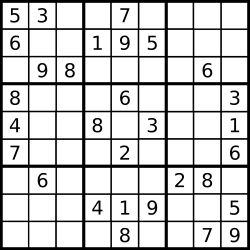
\includegraphics[width=5cm]{sudoku.png}
%% \end{center}

%%%%%%%%%%%%%%%%%%%%%%%%%%%%%%%%%%%%%%%%%%%%%%%%%%%%%%%%%%%%%%%%%%%%%%%%%%%%%%%%

\exerfoot


\section{Literature Pointers}
\providecommand{\slides}{
  \newcommand{\slideshead}{
  \newcommand{\thepage}{\arabic{mypage}}
  %beamer
%  \documentclass[t,hyperref={bookmarks=true}]{beamer}
%  \geometry{papersize={171mm,96mm}}
  \documentclass[t,hyperref={bookmarks=true},aspectratio=169]{beamer}
  \setbeamersize{text margin left=5mm}
  \setbeamersize{text margin right=5mm}
  \usetheme{default}
  \usefonttheme[onlymath]{serif}
  \setbeamertemplate{navigation symbols}{}
  \setbeamertemplate{itemize items}{{\color{black}$\bullet$}}

  \newwrite\keyfile

  %\usepackage{palatino}
  \stdpackages
  %\usepackage{tikz} \usetikzlibrary {shapes.geometric} 
  \usepackage{multimedia}
  \usepackage[utf8]{inputenc}

  \hypersetup{
    colorlinks,
    linkcolor={blue!80!black},
    citecolor={blue!80!black},
    urlcolor={blue!80!black}
  }

  %%% geometry/spacing issues
  %\renewcommand{\baselinestretch}{1.1}
  \renewcommand{\arraystretch}{1.2}
  \columnsep 0mm

  \columnseprule 0pt
  \parindent 0ex
  \parskip 0ex
  %\setlength{\itemparsep}{3ex}
  %\renewcommand{\labelitemi}{\rule[3pt]{10pt}{10pt}~}
  %\renewcommand{\labelenumi}{\textbf{(\arabic{enumi})}}
  \setbeamertemplate{enumerate item}{(\roman{enumi})}
  \newcommand{\headerfont}{\helvetica{14}{1.5}{b}{n}}
  \newcommand{\slidefont} {\helvetica{11}{1.4}{m}{n}}
  %\newcommand{\codefont} {\helvetica{8}{1.2}{m}{n}}
  \newcommand{\urlfont} {\fontsize{6}{1.1}\selectfont}
  \renewcommand{\small} {\helvetica{10}{1.4}{m}{n}}
  \renewcommand{\tiny} {\helvetica{8}{1.3}{m}{n}}
  \newcommand{\ttiny} {\helvetica{7}{1.3}{m}{n}}

  %%% count pages properly and put the page number in bottom right
  %
  \newcounter{mypage}
  \newcommand{\incpage}{\addtocounter{mypage}{1}\setcounter{page}{\arabic{mypage}}}
  \setcounter{mypage}{0}
  \resetcounteronoverlays{page}

  \pagestyle{fancy}
  %\setlength{\headsep}{10mm}
  %\addtolength{\footheight}{15mm}
  \renewcommand{\headrulewidth}{0pt} %1pt}
  \renewcommand{\footrulewidth}{0pt} %.5pt}
  \cfoot{}
  \rhead{}
  \lhead{}
  %% \lfoot{\vspace*{-3mm}\hspace*{-3mm}\helvetica{5}{1.3}{m}{n}{\texttt{github.com/MarcToussaint/AI-lectures}}}
\lfoot{}
%  \rfoot{{\tiny\textsf{AI -- \topic -- \subtopic -- \arabic{mypage}/\pageref{lastpage}}}}
  %\lfoot{\raisebox{5mm}{\tiny\textsf{\slideauthor}}}
  %\rfoot{\raisebox{5mm}{\tiny\textsf{\slidevenue{} -- \arabic{mypage}/\pageref{lastpage}}}}
  %\rfoot{~\anchor{30,12}{\tiny\textsf{\thepage/\pageref{lastpage}}}}
  %\lfoot{\small\textsf{Marc Toussaint}}
  \rfoot{\vspace*{-4.5mm}{\tiny\textsf{\color{gray}\topic\ -- \subtopic\ -- \arabic{mypage}/\pageref{lastpage}}}\hspace*{-4mm}}
%  \rfoot{\vspace*{-4.5mm}{\tiny\textsf{\color{gray}\topic\ -- \arabic{mypage}/\pageref{lastpage}}}\hspace*{-4mm}}
%  \rfoot{~\anchor{-10,12}{\tiny\textsf{\color{gray}\topic\ --  \arabic{mypage}/\pageref{lastpage}}}}
  \lfoot{\vspace*{-4.5mm}{\hspace*{-4mm}\includegraphics[height=4mm]{LIS-26-text-long}}}

  \definecolor{grey}{rgb}{.8,.8,.8}
  \definecolor{head}{rgb}{.85,.9,.9}
%  \definecolor{blue}{rgb}{.0,.0,.5}
%  \definecolor{green}{rgb}{.0,.5,.0}
  \definecolor{red}{rgb}{.8,.0,.0}
  \definecolor{citcol}{gray}{.6}
  \newcommand{\inverted}{
    \definecolor{main}{rgb}{1,1,1}
    \color{main}
    \pagecolor[rgb]{.3,.3,.3}
  }
  \input{../latex/macros}

  \graphicspath{{pics/}{../pics/}{pics-local/}}
}

\newcommand{\slidestitle}{
  \title{\course \topic}
  \author{Marc Toussaint}
  \institute{Learning \& Intelligent Systems Lab, TU Berlin}

  \begin{document}


  %% title slide!
  \slide{}{
    \thispagestyle{empty}

    \twocol{.35}{.55}{
      %\vspace*{-5mm}%
      \hspace*{-5mm}%
      \includegraphics[width=1.\columnwidth]{\coursepicture}
    }{\center

      \textbf{\fontsize{17}{20}\selectfont \course}

      ~

      %Lecture
      \topic\\

      \vspace{1cm}

      {\tiny~\emph{\keywords}~\\}

      \vspace{1cm}

      \teacher
      
      Technical University of Berlin

      \coursedate

      ~

    }
  }
}

\newcommand{\slide}[2]{
  \slidefont
  \incpage\begin{frame}
  \addcontentsline{toc}{section}{#1}
  \vfill
  {\headerfont #1} \vspace*{-2ex}
  \begin{itemize}\item[]~\\
    #2
  \end{itemize}
  \vfill
  \end{frame}
}

% use \begin{frame}[fragile] around slidecore!
\newenvironment{slidecore}[1]{
  \slidefont\incpage
  \addcontentsline{toc}{section}{#1}
  \vfill
  {\headerfont #1} \vspace*{-2ex}
  \begin{itemize}\item[]~\\
}{
  \end{itemize}
  \vfill
}

\newcommand{\titleslide}[4][Marc Toussaint]{
  \newcommand{\slideauthor}{#1}
  \newcommand{\slidevenue}{#3}
  \slidefont
  \incpage
  \begin{frame}
  \begin{center}
    \vspace*{15mm}

    {\headerfont #2\\}
        
    \vspace*{10mm}

    #1 \\

    \vspace*{5mm}

    {\small
      Learning \& Intelligent Systems Lab, TU Berlin\\
%      Science of Intelligence Cluster of Excellence, Berlin\\
      Max Planck Fellow, Institute for Intelligent Systems\\ %Physical Reasoning \& Manipulation Lab -- 
%      MIT CSAIL\\
%      mtoussai@mit.edu,~ marc.toussaint@informatik.uni-stuttgart.de

      \vspace*{10mm}

      \emph{#3}
    }

    \vspace*{0mm}

    %\includegraphics[scale=.1]{pics/eushield-fullcolour}

  \end{center}
  \begin{itemize}\item[]~\\
    #4
  \end{itemize}
  \end{frame}
}

\newcommand{\titleslideempty}[2]{
  \slidefont
  \incpage
  \begin{frame}
  \begin{center}
    \vspace*{15mm}

    {\headerfont #1\\}
        
    %% \vspace*{5mm}

    %% {\small\emph{#2}} \\

  \end{center}
  \begin{itemize}\item[]~\\
    #2
  \end{itemize}
  \end{frame}
}

\providecommand{\key}[1]{
  \addtocounter{mypage}{1}
% \immediate\write\keyfile{#1}
  \addtocontents{toc}{\hyperref[key:#1]{#1 (\arabic{mypage})}}
%  \phantomsection\label{key:#1}
%  \index{#1@{\hyperref[key:#1]{#1 (\arabic{mysec}:\arabic{mypage})}}|phantom}
  \addtocounter{mypage}{-1}
}

\providecommand{\course}{}

\providecommand{\subtopic}{}

\providecommand{\sublecture}[2]{
  \renewcommand{\subtopic}{#1}
  \slide{#1}{#2}
}

\providecommand{\sublectureHide}[2]{
  \renewcommand{\subtopic}{#1}
}

\providecommand{\story}[1]{
~

Motivation: {\tiny #1}\clearpage
}

\newenvironment{items}[1][9]{
\par\setlength{\unitlength}{1pt}\fontsize{#1}{#1}\linespread{1.2}\selectfont
\begin{list}{--}{\leftmargin4ex \rightmargin0ex \labelsep1ex \labelwidth2ex
\topsep.7ex \parsep0ex \itemsep3pt}
}{
\end{list}
}

\newenvironment{itemS}[1][4ex]{
\par
\tiny
\begin{list}{--}{\leftmargin#1 \rightmargin0ex \labelsep1ex
  \labelwidth2ex \topsep0pt \parsep0ex \itemsep2pt}
}{
\end{list}
}

\providecommand{\slidesfoot}{
  \end{document}
}


  \slideshead
  \lecturetitleslide
}

\providecommand{\exercises}{
  \newcommand{\exerciseshead}{
  \documentclass[10pt,fleqn]{article}
  \stdpackages
\usepackage[utf8]{inputenc}

  \definecolor{bluecol}{rgb}{0,0,.5}
  \definecolor{greencol}{rgb}{0,.4,0}
  \definecolor{shadecolor}{gray}{0.9}
  \usepackage[
    %    pdftex%,
    %%    letterpaper,
    %    bookmarks,
    %    bookmarksnumbered,
    colorlinks,
    urlcolor=bluecol,
    citecolor=black,
    linkcolor=bluecol,
    %    pagecolor=bluecol,
    pdfborder={0 0 0},
    %pdfborderstyle={/S/U/W 1},
    %%    backref,     %link from bibliography back to sections
    %%    pagebackref, %link from bibliography back to pages
    %%    pdfstartview=FitH, %fitwidth instead of fit window
    pdfpagemode=UseNone, %UseOutlines, %bookmarks are displayed by acrobat
    pdftitle={\course},
    pdfauthor={Marc Toussaint},
    pdfkeywords={}
  ]{hyperref}
  \DeclareGraphicsExtensions{.pdf,.png,.jpg,.eps}

  \renewcommand{\r}{\varrho}
  \renewcommand{\l}{\lambda}
  \renewcommand{\L}{\Lambda}
  \renewcommand{\b}{\beta}
  \renewcommand{\d}{\delta}
  \renewcommand{\k}{\kappa}
  \renewcommand{\t}{\theta}
  \renewcommand{\O}{\Omega}
  \renewcommand{\o}{\omega}
  \renewcommand{\SS}{{\cal S}}
  \renewcommand{\=}{\!=\!}
  %\renewcommand{\boldsymbol}{}
  %\renewcommand{\Chapter}{\chapter}
  %\renewcommand{\Subsection}{\subsection}

  \renewcommand{\baselinestretch}{1.1}
  \geometry{a4paper,headsep=7mm,hdivide={15mm,*,15mm},vdivide={20mm,*,15mm}}

  \fancyhead[L]{\thetitle, \textit{\teacher}---\coursedate}
  \fancyhead[R]{\thepage}
  \fancyhead[C]{}
  \fancyfoot{}
  \pagestyle{fancy}

  \renewcommand{\labelenumi}{{\alph{enumi})}}

  \parindent 0pt
  \parskip 0.5ex

  \newcommand{\codefont}{\helvetica{8}{1.2}{m}{n}}
  \newcommand{\urlfont} {\fontsize{6}{1.1}\selectfont}
  \newcommand{\ttiny} {\helvetica{7}{1.3}{m}{n}}

  \input{../latex/macros}

  \DefineShortVerb{\@}

  \usepackage{comment}
  \specialcomment{solution}{
    \small
    \begin{shaded}
  }{
    \end{shaded}
  }
  
  \renewcommand{\hat}{\widehat}
  \newcommand{\bbg}{{\bar{\bar g}}}
  \graphicspath{{pics/}{../pics/}}

  \mytitle{\course\\\exnum}
  \myauthor{\teacher\\ \small\addressTUB}
  \date{\coursedate}
}

%%%%%%%%%%%%%%%%%%%%%%%%%%%%%%%%%%%%%%%%%%%%%%%%%%%%%%%%%%%%%%%%%%%%%%%%%%%%%%%%

\newcommand{\exercisestitle}{  
  \begin{document}
  \maketitle
}

\newcommand{\exsection}[1]{\section{#1}}

\newcommand{\exsubsection}[1]{\subsection{#1}}

\newcommand{\exerfoot}{
  \end{document}
}

\newenvironment{items}[1][9]{
  \par\setlength{\unitlength}{1pt}\fontsize{#1}{#1}\linespread{1.2}\selectfont
  \begin{list}{--}{\leftmargin4ex \rightmargin0ex \labelsep1ex \labelwidth2ex
      \topsep0pt \parsep0ex \itemsep3pt}
}{
  \end{list}
}

  \exerciseshead
}

\providecommand{\script}{
  \newcommand{\scripthead}{
  \documentclass[9pt,fleqn,twoside]{article}
  \stdpackages

  \usepackage{makeidx}
  \makeindex

  \usepackage{thmtools}
  \definecolor{shadecolor}{gray}{0.85}
  \declaretheoremstyle[
    %headfont=\normalfont\bfseries,
    %notefont=\mdseries, notebraces={(}{)},
    %bodyfont=\normalfont,
    %postheadspace=0.5em,
    %spaceabove=6pt,
    mdframed={
      %  skipabove=8pt,
      %  skipbelow=6pt,
      hidealllines=true,
      backgroundcolor={shadecolor},
      innertopmargin=8pt,
      %  innerleftmargin=3pt,
      %  innerrightmargin=3pt
    }
  ]{shaded}
  \declaretheorem[style=shaded,within=section,name=Definition]{myDefinition}
  \declaretheorem[style=shaded,within=section,name=Theorem]{myTheorem}
  \declaretheorem[style=shaded,within=section,name=Identities]{Identities}
  \declaretheorem[style=shaded,within=section,name=Example]{myExample}

  \definecolor{grey}{rgb}{.8,.8,.8}
  \definecolor{bluecol}{rgb}{0,0,.5}
  \definecolor{greencol}{rgb}{0,.4,0}
  \definecolor{shadecolor}{gray}{0.9}
  \definecolor{citcol}{rgb}{.4,.4,.4}
  \usepackage[
    %    pdftex%,
    %%    letterpaper,
    %bookmarks,
    bookmarksnumbered,
    colorlinks,
    urlcolor=bluecol,
    citecolor=black,
    linkcolor=bluecol,
    %    pagecolor=bluecol,
    pdfborder={0 0 0},
    %pdfborderstyle={/S/U/W 1},
    %%    backref,     %link from bibliography back to sections
    %%    pagebackref, %link from bibliography back to pages
    %%    pdfstartview=FitH, %fitwidth instead of fit window
    pdfpagemode=UseOutlines, %bookmarks are displayed by acrobat
    pdftitle={\course},
    pdfauthor={Marc Toussaint},
    pdfkeywords={}
  ]{hyperref}
  \DeclareGraphicsExtensions{.pdf,.png,.jpg,.eps}

  %\usepackage{multirow}
  \usepackage{multimedia}
  %\usepackage{marginnote}
  %\setbeamercolor{background canvas}{bg=}

  \usepackage[round]{natbib}
  \bibliographystyle{abbrvnat}

  \renewcommand{\r}{\varrho}
  \renewcommand{\l}{\lambda}
  \renewcommand{\L}{\Lambda}
  \renewcommand{\b}{\beta}
  \renewcommand{\d}{\delta}
  \renewcommand{\k}{\kappa}
  \renewcommand{\t}{\theta}
  \renewcommand{\O}{\Omega}
  \renewcommand{\o}{\omega}
  \renewcommand{\SS}{{\cal S}}
  \renewcommand{\=}{\!=\!}
  %\renewcommand{\boldsymbol}{}
  %\renewcommand{\Chapter}{\chapter}
  %\renewcommand{\Subsection}{\subsection}

  \renewcommand{\baselinestretch}{1.0}
  \geometry{a5paper,headsep=6mm,hdivide={10mm,*,10mm},vdivide={13mm,*,7mm}}

  \fancyhead[OL,ER]{\course, \textit{Marc Toussaint}}
  \fancyhead[OR,EL]{\thepage}
  \fancyhead[C]{}
  \fancyfoot{}
  \pagestyle{fancy}

  \renewcommand{\labelenumi}{{(\roman{enumi})}}
  \renewcommand{\theenumi}{(\roman{enumi})} %for ref
  \parindent 0pt
  \parskip .5pc

  \columnsep 6ex

  \renewcommand{\familydefault}{\sfdefault}

  \newcommand{\headerfont}{\large}%helvetica{12}{1}{b}{n}}
  \newcommand{\slidefont} {}%\helvetica{9}{1.3}{m}{n}}
  \newcommand{\storyfont} {}
  %  \renewcommand{\small}   {\helvetica{8}{1.2}{m}{n}}
  \renewcommand{\tiny}    {\footnotesize}%helvetica{7}{1.1}{m}{n}}
  \newcommand{\ttiny} {\footnotesize}%fontsize{7}{7}\selectfont}
%  \newcommand{\codefont}{\fontsize{6}{6}\selectfont}%helvetica{8}{1.2}{m}{n}}
  \newcommand{\codefont} {\helvetica{8}{1.2}{m}{n}}

  \input{../latex/macros}

  \usepackage{comment}
  \specialcomment{solution}{
    \small
    \begin{shaded}
  }{
    \end{shaded}
  }

  \graphicspath{{pics/}{../latex/pics/}}

  \mytitle{\course\\Lecture Script}
  \myauthor{Marc Toussaint}
  \date{\coursedate}
}

%%%%%%%%%%%%%%%%%%%%%%%%%%%%%%%%%%%%%%%%%%%%%%%%%%%%%%%%%%%%%%%%%%%%%%%%%%%%%%%%

\newcommand{\scripttitle}{
  \begin{document}
  \maketitle
  %\anchor{100,10}{\includegraphics[width=4cm]{optim}}
%  \vspace*{1cm}

  \emph{This is a direct concatenation and reformatting of all lecture
    slides and exercises from this course, including indexing to help
    prepare for exams.}

  {\tableofcontents}
}

%%%%%%%%%%%%%%%%%%%%%%%%%%%%%%%%%%%%%%%%%%%%%%%%%%%%%%%%%%%%%%%%%%%%%%%%%%%%%%%%

\newcounter{mypage}
\setcounter{mypage}{0}
\newcommand{\incpage}{\addtocounter{mypage}{1}}

\newcommand{\subtopic}{}
\newcommand{\pause}{}
\newcommand{\only}[1]{#1}

\renewcommand{\slides}[1][]{
  %  \clearpage
  \subsection{\topic}
  \index{\topic}
  {\small #1}
  \setcounter{mypage}{0}
  \smallskip\nopagebreak\hrule\medskip
}

\newcommand{\slidesfoot}{
  \bigskip
}

\newcommand{\sublecture}[2]{
  \index{#1}
}

\newcommand{\key}[1]{
  \phantomsection\addcontentsline{toc}{subsubsection}{#1}
  %\subsubsection{#1}
  \index{#1}
}

\providecommand{\defn}[1]{%
  \textbf{#1}\index{#1}%
}

\newenvironment{slidecore}[1]{
  \incpage
  \subsubsection*{#1}%{\headerfont\noindent\textbf{#1}\\}%
  \vspace{-6ex}%
  \begin{list}{$\bullet$}{\leftmargin4ex \rightmargin0ex \labelsep1ex
    \labelwidth2ex \partopsep0ex \topsep0ex \parsep.5ex \parskip0ex \itemsep0pt}\item[]~\\\nopagebreak%
}{
  \end{list}\nopagebreak%
  {\hfill\tiny \textsf{\arabic{section}.\arabic{subsection}:\arabic{mypage}}}\nopagebreak%
  \smallskip\nopagebreak\hrule
}

\newcommand{\slide}[2]{
  \begin{slidecore}{#1}
    #2
  \end{slidecore}
}

\renewcommand{\exercises}{}
\newcommand{\exercisestitle}{}
\newcommand{\exsection}[1]{\subsubsection{#1}}
\newcommand{\exerfoot}{\bigskip}

\newcommand{\story}[1]{
  \subsection*{Motivation \& Outline}
  {\storyfont\sf #1}
  \medskip\nopagebreak\hrule
}

\newcounter{savedsection}
\newcommand{\subappendix}{\setcounter{savedsection}{\arabic{section}}\appendix}
\newcommand{\noappendix}{
  \setcounter{section}{\arabic{savedsection}}% restore section number
  \setcounter{subsection}{0}% reset section counter
%  \gdef\@chapapp{\sectionname}% reset section name
  \renewcommand{\thesection}{\arabic{section}}% make section numbers arabic
}

\newenvironment{items}[1][9]{
\par\setlength{\unitlength}{1pt}\fontsize{#1}{#1}\linespread{1.2}\selectfont
\begin{list}{--}{\leftmargin4ex \rightmargin0ex \labelsep1ex \labelwidth2ex
\topsep0pt \parsep0ex \itemsep3pt}
}{
\end{list}
}

\newcommand{\Def}[1]{%
\textbf{#1}\index{#1}}%\marginnote{#1}}

  \scripthead
}

\providecommand{\note}{
  \providecommand{\notehead}[2]{
  \documentclass[#1,fleqn,twoside]{article}
  \stdpackages
  \renewcommand{\labelenumi}{{(\roman{enumi})}}
  \renewcommand{\theenumi}{(\roman{enumi})} %for ref

  \renewcommand{\baselinestretch}{#2}
  \renewcommand{\arraystretch}{1.2}
  \renewcommand{\topfraction}{1}
  \renewcommand{\bottomfraction}{1}
  \renewcommand{\textfraction}{0}
  \columnsep 5ex
  \parindent 3ex
  \parskip 1ex

  % Lists and paragraphs
  \parindent 0pt
  \topsep 4pt plus 1pt minus 2pt
  \partopsep 1pt plus 0.5pt minus 0.5pt
  \itemsep 2pt plus 1pt minus 0.5pt
  \parsep 2pt plus 1pt minus 0.5pt
  \parskip .5pc %add _in_ {thebibliography} environment in *.bbl

  \setcounter{tocdepth}{3}
  \setcounter{secnumdepth}{3}

  \geometry{a4paper,hdivide={25mm,*,25mm},vdivide={25mm,*,25mm}}

  \renewcommand{\headrulewidth}{.0pt}\renewcommand{\footrulewidth}{.0pt}\cfoot{}
  \fancyhead[OL,EC]{\it\theauthor---\today}
  \fancyhead[ER]{\leftmark}
  \fancyhead[OR,EL]{\thepage}
  \fancyfoot[EL,OR]{}
  \setlength{\headsep}{10mm}
  %\fancyhead[OL]{\rightmark}
  %\fancyfoot[EL,OR]{}


  %  \usepackage{palatino}

  \newcommand{\codefont}{\helvetica{8}{1.2}{m}{n}}

  \renewenvironment{abstract}{
    \vspace*{5ex}\begin{list}{}{
      \leftmargin3ex
      \rightmargin3ex
      \topsep-\parskip}\item[]
     \hrule\vspace{1.5ex}{\bf Abstract.~}\small}
    {\vspace{2ex}\hrule\end{list}\vspace{5ex}}
    
  \newenvironment{keyword}
    {\par{\it Keywords:~}}
    {}

  \def\makemytitle{%
    \thispagestyle{empty}
    \begin{list}{}{\leftmargin3ex \rightmargin3ex \topsep0ex \parsep0ex}\item[]
      \begin{center}
        {\fontsize{18}{25}\selectfont{\thetitle\\}}\vspace{5ex}

        {\fontsize{14}{16}\selectfont{\theauthor\\}}\vspace{1ex}

        {\footnotesize{\sl \addressFUB}\\ \emailBerlin}

        {\footnotesize \today}

        \vspace{1ex}
        {\small \published}
      \end{center}
    \end{list}
    \renewcommand{\maketitle}{\chapter{\thetitle}}
  }

  \input{../latex/macros}
  \pdflatex

  \graphicspath{{pics/}{../pics/}{pics-local/}}

  \myauthor{Marc Toussaint}
  \date{\today}
}

%%%%%%%%%%%%%%%%%%%%%%%%%%%%%%%%%%%%%%%%%%%%%%%%%%%%%%%%%%%%%%%%%%%%%%%%%%%%%%%%

\newcommand{\notetitle}{
  \begin{document}
  \thispagestyle{empty}
    
  \maketitle

}

\newenvironment{items}[1][9]{
\par\setlength{\unitlength}{1pt}\fontsize{#1}{#1}\linespread{1.2}\selectfont
\begin{list}{--}{\leftmargin4ex \rightmargin0ex \labelsep1ex \labelwidth2ex
\topsep0pt \parsep0ex \itemsep3pt}
}{
\end{list}
}

  \notehead{10}{1.1}
}

\providecommand{\course}{NO COURSE}
\providecommand{\coursepicture}{NO PICTURE}
\providecommand{\coursedate}{NO DATE}
\providecommand{\topic}{NO TOPIC}
\providecommand{\keywords}{NO KEYWORDS}
\providecommand{\exnum}{NO NUMBER}
\providecommand{\teacher}{Marc Toussaint}

\providecommand{\stdpackages}{
  \usepackage{amsmath}
  \usepackage{amssymb}
  \usepackage{amsfonts}
  \allowdisplaybreaks
  \usepackage{amsthm}
  \usepackage{eucal}
  \usepackage{graphicx}
  \usepackage{color}
  \usepackage{geometry}
  \usepackage{framed}
%  \usecolor{xcolor}
  \definecolor{shadecolor}{gray}{0.9}
  \setlength{\FrameSep}{3pt}
  \usepackage{fancyvrb}
  \fvset{numbers=none,xleftmargin=5ex}

  \usepackage{pdfpages}

  \usepackage{multicol} 
  \usepackage{fancyhdr}
}

\providecommand{\addressUSTT}{
  Machine~Learning~\&~Robotics~lab, U~Stuttgart\\\small
  Universit{\"a}tsstra{\ss}e 38, 70569~Stuttgart, Germany
}

\providecommand{\addressTUB}{
  Learning~\&~Intelligent~Systems~Lab, TU~Berlin\\\small
  Marchstr. 23, 10587 Berlin, Germany
}


\renewcommand{\course}{Artificial Intelligence}
\renewcommand{\coursepicture}{course_ai}
\renewcommand{\coursedate}{Summer 2023}

\renewcommand{\exnum}{Literature Recommendations}

\exercises
\excludecomment{solution}
\exercisestitle

%%%%%%%%%%%%%%%%%%%%%%%%%%%%%%%%%%%%%%%%%%%%%%%%%%%%%%%%%%%%%%%%%%%%%%%%%%%%%%%%

\begin{itemize}
\item Maths notation, basic definitions, derivatives, etc:
\begin{items}
\item \href{https://www.user.tu-berlin.de/mtoussai/teaching/Lecture-Maths.pdf}{Maths for Intelligent Systems} (Brief reference for Linear Algebra, Optimization \& Probabilities)
\end{items}

\item Probabilities:
\begin{items}
\item Basics: Bishop (Pattern Recognition and Machine Learning), section 1.2 (until 1.2.4), available online (just google, or visit Bishop's page:
\url{https://www.microsoft.com/en-us/research/wp-content/uploads/2006/01/Bishop-Pattern-Recognition-and-Machine-Learning-2006.pdf})
\end{items}

\item Machine Learning:
\begin{items}
\item Bishop \& Bishop: Deep Learning: Foundations and Concepts. Springer, 2023
\item Hastie et al:The Elements of Statistical Learning: Data Mining, Inference, and Prediction
Springer, 2009. Esp.\ section 2.3. \url{https://hastie.su.domains/ElemStatLearn/}
\item own script: \href{https://www.user.tu-berlin.de/mtoussai/teaching/Lecture-MachineLearning.pdf}{Introduction to Machine Learning}, section 2
\end{items}

\item Decision Theory
\begin{items}
\item Russel \& Norwig chapter 16 (\url{https://zoo.cs.yale.edu/classes/cs470/materials/aima2010.pdf})
\end{items}

\item Monte Carlo
\begin{items}
\item Wikipedia (German version!) good; english version good but inconcise
\url{https://de.wikipedia.org/wiki/Monte-Carlo-Simulation}
\item Best, but perhaps too advanced: \emph{An Introduction to MCMC for Machine Learning} \url{https://www.cs.ubc.ca/~arnaud/andrieu_defreitas_doucet_jordan_intromontecarlomachinelearning.pdf}
\item Sampling in general: Bishop Chapter 11
\item Russel \& Norwig mentions Monte Carlo simulation, but not very helpful
\end{items}

\item MCTS
\begin{items}
\item Browne et al.: \emph{A Survey of Monte Carlo Tree Search Methods}, 2012.
\item ICAPS'10 Tutorial:
\url{http://web.engr.oregonstate.edu/~afern/icaps10-MCP-tutorial.ppt}
\end{items}

\item MDPs, Value Iteration \& Reinforcement Learning
\begin{items}
\item Sutton \& Barto is the standard reference \url{https://web.stanford.edu/class/psych209/Readings/SuttonBartoIPRLBook2ndEd.pdf}. Chapter 4 for basics on MDPs \& Value Iteration; Chapters 6 \& 7 are the classics for model-free Reinforcement Learning
\end{items}

\item More General Pointers
\begin{items}
\item A list on Linear Algebra, Probabilities, ML basics, \& Optimization:
\url{https://www.user.tu-berlin.de/mtoussai/teaching/#reference-material}
\end{items}

\end{itemize}

%%%%%%%%%%%%%%%%%%%%%%%%%%%%%%%%%%%%%%%%%%%%%%%%%%%%%%%%%%%%%%%%%%%%%%%%%%%%%%%%

\exerfoot



%%%%%%%%%%%%%%%%%%%%%%%%%%%%%%%%%%%%%%%%%%%%%%%%%%%%%%%%%%%%%%%%%%%%%%%%%%%%%%%%

\clearpage
\phantomsection
\addtocontents{toc}{\par}
\addcontentsline{toc}{section}{Index}
\printindex

\end{document}

